% Copyright (c) 2022 by Lars Spreng
% This work is licensed under the Creative Commons Attribution 4.0 International License. 
% To view a copy of this license, visit http://creativecommons.org/licenses/by/4.0/ or send a letter to Creative Commons, PO Box 1866, Mountain View, CA 94042, USA.

%~~~~~~~~~~~~~~~~~~~~~~~~~~~~~~~~~~~~~~~~~~~~~~~~~~~~~~~~~~~~~~~~~~~~~~~~~~~~~~
% You can add your packages and commands to the loadslides.tex file. 
% The files in the folder "styles" can be modified to change the layout and design of your slides.
% I have included examples on how to use the template below. 
% Some of these examples are taken from the Metropolis template.
%~~~~~~~~~~~~~~~~~~~~~~~~~~~~~~~~~~~~~~~~~~~~~~~~~~~~~~~~~~~~~~~~~~~~~~~~~~~~~~


\documentclass[
11pt,notheorems,hyperref={pdfauthor=whatever}
]{beamer}

\input{loadslides.tex} % Loads packages and some defined commands

\title[
% Text entered here will appear in the bottom middle
]{Emisión de paquetes de $n$-fonones en una molécula excitónica mediante procesos de Stokes}


\author[Jhon S. García Barrera]{
	Jhon S. García Barrera \\[0.5em]
}

\institute{
	%\textit{Directores:} \\
	%Edgar A. Gómez G. \\ Santiago Echeverri Arteaga  \\[1.5em]
	Facultad de Ciencias Básicas y Tecnologías, \\
	Programa de Física, \\
	Universidad del Quindío
}
\date{\today}

\begin{document}

% Generate title page
{
\setbeamertemplate{footline}{} 
\begin{frame}
  \titlepage
\end{frame}
}
\addtocounter{framenumber}{-1}

% You can declare different parts as a parentof sections
\begin{frame}{Contenido}
	\tableofcontents
\end{frame}

\section{Introducción}
\begin{frame}{Motivación}
	
	\begin{columns}[T]
		
		\begin{column}{0.52\textwidth}
			\vspace{6pt}
			Los \textbf{estados cuánticos de $n$ fotones} son recursos
			fundamentales para tecnologías cuánticas:\\[8pt]
			\begin{itemize}
				\item \textbf{Metrología:} interferometría sub-Heisenberg
				con estados de Fock ópticos
				\item \textbf{Criptografía:} protocolos QKD basados en
				fuentes de fotón único
				\item \textbf{Computación:} puertas cuánticas lineales
				ópticas (KLM) con estados de $n$ fotones
				\item \textbf{Sensado:} superresolución en microscopía
				NOON y litografía cuántica
			\end{itemize}
			
			\vspace{8pt}
			{\small
				Sin embargo, generar estados de $n$ fotones de forma
				\textbf{determinista y con alta pureza} sigue siendo
				un problema abierto: la eficiencia cae exponencialmente con $n$.
			}
		\end{column}
		
		\begin{column}{0.44\textwidth}
			\vspace{10pt}
			\begin{center}
				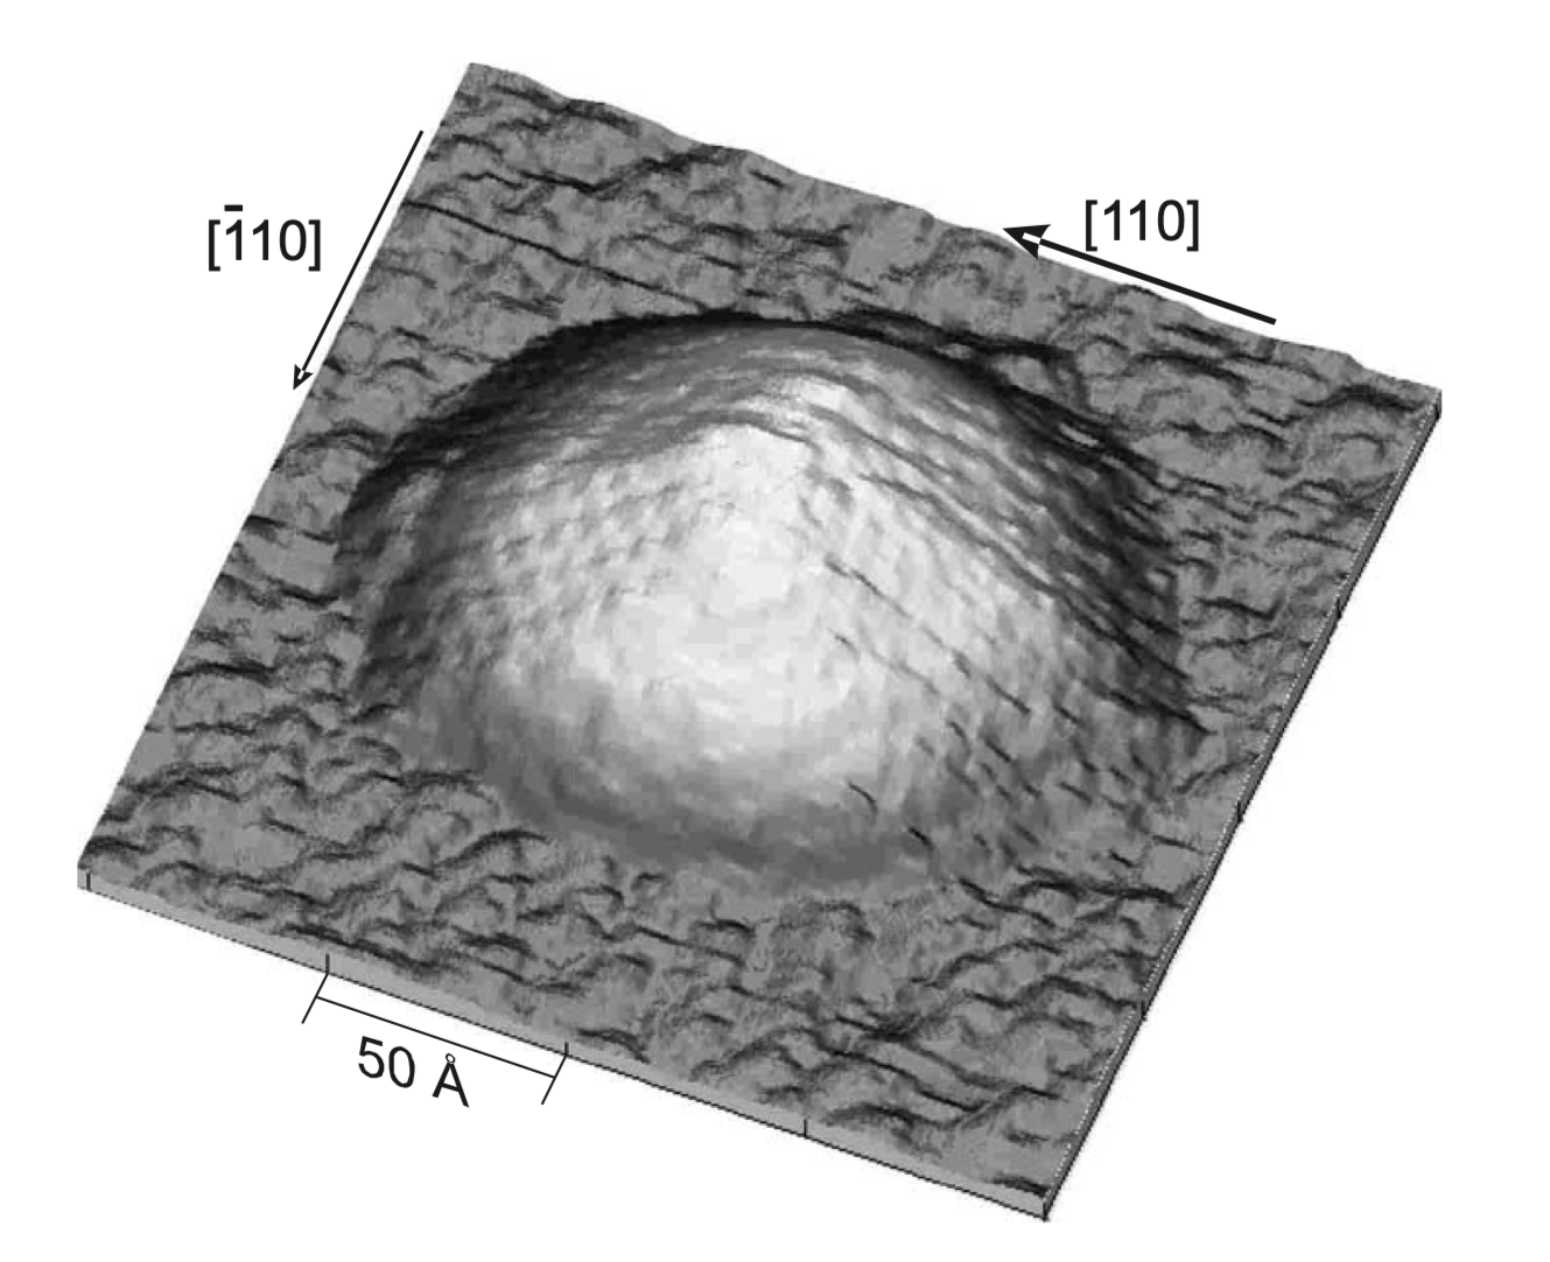
\includegraphics[width=0.85\textwidth]{img/QD.png}\\[6pt]
				{\scriptsize Imagen STM de un punto cuántico
					de InAs/GaAs \cite{eisele2008}.}
			\end{center}
		\end{column}
		
	\end{columns}
	
\end{frame}

\begin{frame}{Antecedentes I: emisión de paquetes de fotones}
	
	\textbf{Emitters of $N$-photon bundles}\\
	{\footnotesize Muñoz et al., \textit{Nat. Photonics} \textbf{8},
		550 (2014) \cite{munoz2014}}
	
	\begin{columns}[T]
		
		\begin{column}{0.44\textwidth}			
			\vspace{25pt}
			\begin{itemize}
				\item Un TLS en cavidad emite luz \textbf{exclusivamente
					en grupos de $N$ fotones}, con $N$ controlado
				por la frecuencia del láser.
				\item Introduce la \textbf{pureza} $\pi_N$ y las
				funciones $g_N^{(n)}$ como observables propios
				de paquetes.
				\item Demuestra $\pi_2 \approx 99\%$ en condiciones
				óptimas de cQED.
			\end{itemize}
		\end{column}
		
		\begin{column}{0.52\textwidth}
			\vspace{-15pt}
			\begin{center}
				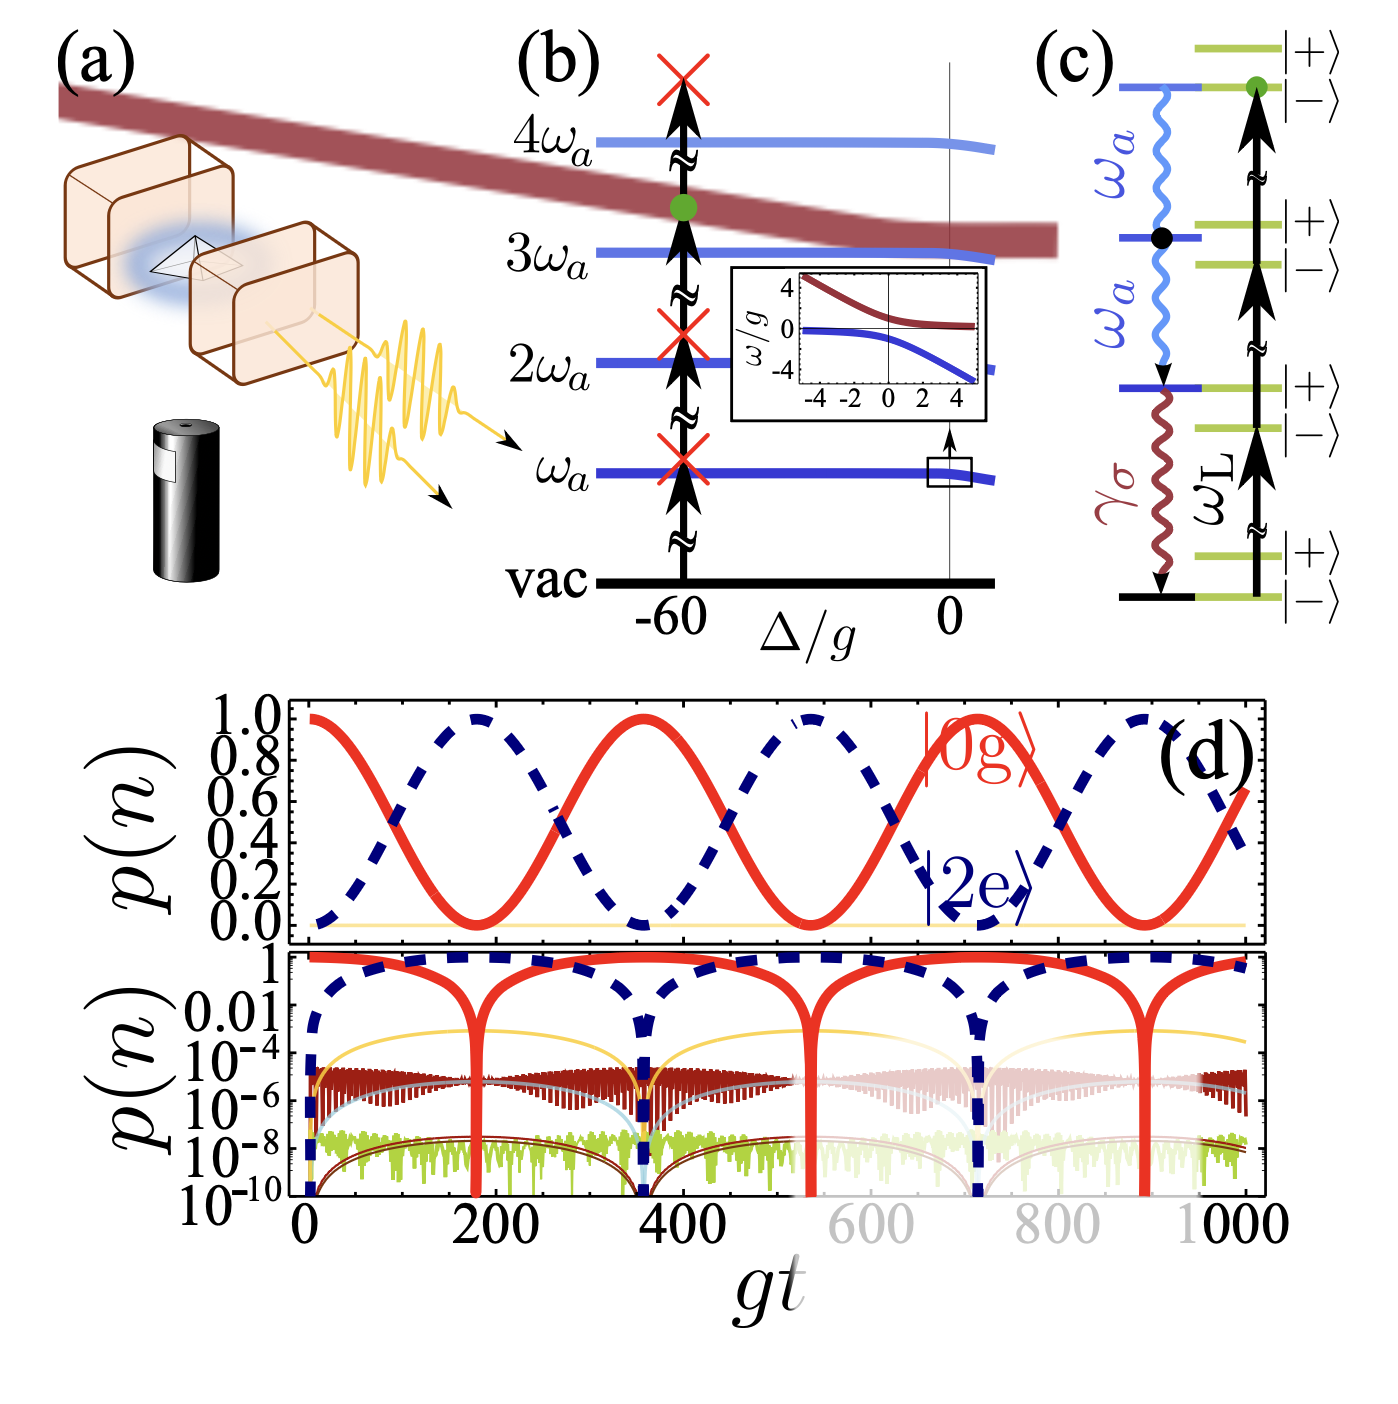
\includegraphics[width=0.70\textwidth]{img/munoz2014.png}\\[4pt]
				{\scriptsize Esquema del sistema y estructura de energía
					para emisión de paquetes de $N$ fotones \cite{munoz2014}.}
			\end{center}
		\end{column}
		
	\end{columns}
	
\end{frame}

\begin{frame}{Antecedentes II: filtrado y mejora de pureza}
	
	\textbf{Filtering multiphoton emission from state-of-the-art cavity QED}\\
	{\footnotesize Muñoz et al., \textit{Optica} \textbf{5}, 14 (2018)
		\cite{munoz2018}}
	
	\begin{columns}[T]
		
		\begin{column}{0.52\textwidth}
			\begin{center}
				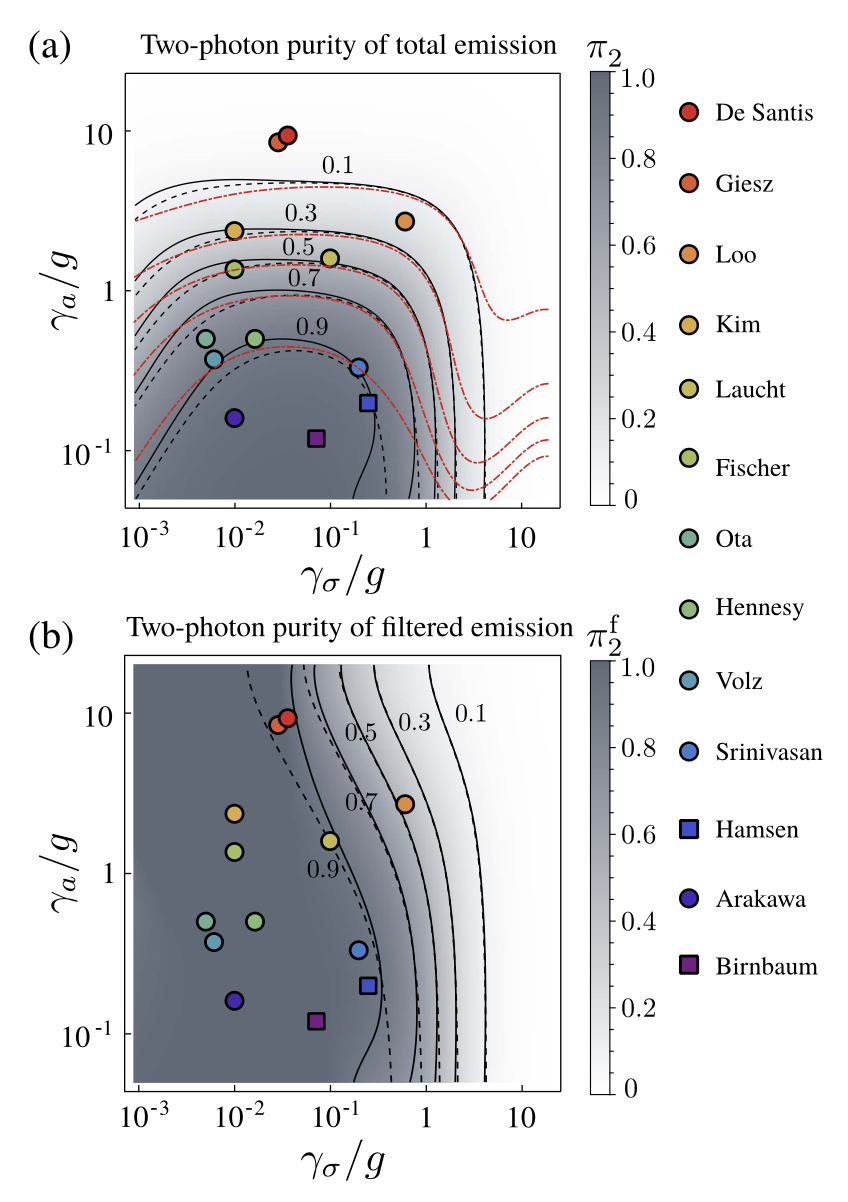
\includegraphics[width=0.55\textwidth]{img/munoz2018.png}\\[4pt]
				{\scriptsize Pureza $\pi_2$ sin filtrar (a) y filtrada
					$\pi_2^f$ (b) en el espacio $(\gamma_a, \gamma_\sigma)/g$.
					El filtrado amplía drásticamente la región de alta
					pureza \cite{munoz2018}.}
			\end{center}
		\end{column}
		
		\begin{column}{0.44\textwidth}
			\vspace{29pt}
			\begin{itemize}
				\item El mismo sistema, pero los fotones espurios
				y los paquetes de $N$ fotones se emiten en
				\textbf{ventanas espectrales distintas}.
				\item Un filtro en frecuencia suprime la
				contaminación de fotón único y
				\textbf{relaja el requisito de acoplamiento fuerte}
				al régimen \textit{bad-cavity} ($C > 1$).
				\item Abre la implementación en semiconductores
				y átomos en nanofotónica.
			\end{itemize}
		\end{column}
		
	\end{columns}
	
\end{frame}

\begin{frame}{Antecedentes: ¿por qué fonones?}
	
	\textbf{$N$-Phonon Bundle Emission via Stokes Process}\\
	{\footnotesize Bin et al., \textit{Phys. Rev. Lett.} \textbf{124}, 053601 (2020) \cite{bin2020}}
	
	\vspace{12pt}
	
	{\small
		\begin{itemize}\setlength{\itemsep}{12pt}
			
			\item \textbf{Velocidad de propagación:} las ondas acústicas
			se propagan significativamente más lento que la luz,
			lo que las hace idóneas para comunicaciones cuánticas
			en chip sobre distancias de unos pocos cientos de
			micrómetros o menos \cite{gustafsson2014,kuzyk2018}.
			
			\item \textbf{Sin pérdidas por radiación:} dado que los
			fonones solo pueden propagarse en un medio material,
			no sufren las pérdidas radiativas que afectan a los
			fotones en guías de onda ópticas.
			
			\item \textbf{Alta sintonizabilidad:} las cavidades
			fonónicas han sido demostradas experimentalmente
			en un rango que va desde GHz hasta THz
			\cite{weig2004,rozas2009,oconnell2010,macCabe2020,zalalutdinov2021},
			cubriendo un espectro de frecuencias amplio y
			experimentalmente accesible.
			
			\item \textbf{Compatibilidad con técnicas de estado
				sólido:} las numerosas herramientas desarrolladas
			por la física de estado sólido
			\cite{ask2019,kharel2018,xu2018,akimov2017}
			se vuelven directamente disponibles para tareas
			de procesamiento de información cuántica con
			fonones \cite{manenti2017,wan2021}.
			
		\end{itemize}
	}
	
\end{frame}

\section{Objetivos}

\begin{frame}{Objetivos}
	
	\textbf{Objetivo general}\\[4pt]
	Analizar la emisión multifonónica en una molécula excitónica acoplada a una cavidad acústica bajo resonancia de Stokes, determinando cómo la hibridación excitónica modifica la pureza y la estabilidad paramétrica de los paquetes de fonones generados.
	
	\vspace{8pt}
	\textbf{Objetivos específicos}
	\begin{itemize}
		\item Formular el modelo teórico y derivar las condiciones de resonancia de Stokes y las frecuencias super-Rabi efectivas del sistema 2QD.
		\item Implementar la ecuación maestra de Lindblad en \textsc{QuTiP} y calcular $g^{(n)}(0)$ y las purezas de emisión $\Pi_n$ ($n=2,3,4$), caracterizando la estadística de los paquetes de fonones emitidos.
		\item Comparar sistemáticamente con el esquema de un único punto cuántico, identificando efectos emergentes del acoplamiento excitónico coherente.
	\end{itemize}
	
\end{frame}

\section{Modelo}
\begin{frame}{Modelo y Hamiltoniano}
	
			{\small
		\begin{equation*}
			H_{\mathrm{lab}}
			= \omega_b b^\dagger b
			+ \omega_\sigma \!\left(\sigma_1^\dagger\sigma_1+\sigma_2^\dagger\sigma_2\right)
			+ \lambda\!\left(\sigma_1^\dagger\sigma_1+\sigma_2^\dagger\sigma_2\right)\!(b^\dagger+b)
			+ J\!\left(\sigma_1^\dagger\sigma_2+\sigma_2^\dagger\sigma_1\right)
			+ \Omega\!\sum_{i=1,2}\!\left(e^{i\omega_L t}\sigma_i+e^{-i\omega_L t}\sigma_i^\dagger\right)
		\end{equation*}
	}
	
	\vspace{6pt}
	\rule{\textwidth}{0.4pt}
	\vspace{2pt}
	
	\begin{columns}[T]
		
		% ── Columna izquierda: marco rotante ──────────────────────────
		\begin{column}{0.42\textwidth}
			\vspace{6pt}
			\textbf{Marco rotante}\\[6pt]
			Operador unitario:
			\begin{equation*}
				U(t) = \exp\!\left(i\omega_L t \left(\sigma_1^\dagger\sigma_1
				+ \sigma_2^\dagger\sigma_2\right)\right)
			\end{equation*}
			\begin{equation*}
				H = U\,H_{\mathrm{lab}}\,U^\dagger + i\,\dot{U}\,U^\dagger
			\end{equation*}
			\vspace{4pt}
	
		\end{column}
		
		% ── Columna derecha: TikZ ─────────────────────────────────────
		\begin{column}{0.45\textwidth}
			\vspace{-6pt}
			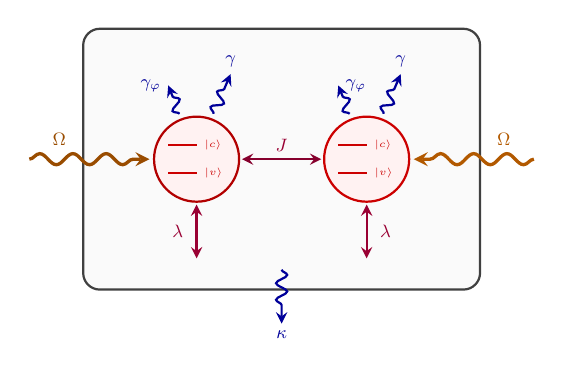
\begin{tikzpicture}[>=stealth, thick, font=\small,
				scale=0.72, transform shape,
				diss/.style={->, thick, decorate,
					decoration={snake, amplitude=2pt, segment length=6pt,
						post length=4pt}},
				coup/.style={<->, thick}]
				
				\draw[gray!50!black, thick, rounded corners=6pt, fill=gray!4]
				(-3.5,-1.0) rectangle (3.5,3.6);
				
				\def\CH{1.2}\def\QDY{1.3}\def\QDX{1.5}\def\QDR{0.75}
				
				% QD1
				\draw[red!70!black, thick, fill=red!5]
				(-\QDX,\QDY) circle (\QDR);
				\draw[red!80!black, thick]
				(-\QDX-0.50,\QDY-0.25) -- (-\QDX+0.01,\QDY-0.25)
				node[right,font=\tiny]{$|v\rangle$};
				\draw[red!80!black, thick]
				(-\QDX-0.50,\QDY+0.25) -- (-\QDX+0.01,\QDY+0.25)
				node[right,font=\tiny]{$|c\rangle$};
				
				% QD2
				\draw[red!80!black, thick, fill=red!5]
				(\QDX,\QDY) circle (\QDR);
				\draw[red!80!black, thick]
				(\QDX-0.50,\QDY-0.25) -- (\QDX+0.01,\QDY-0.25)
				node[right,font=\tiny]{$|v\rangle$};
				\draw[red!80!black, thick]
				(\QDX-0.50,\QDY+0.25) -- (\QDX+0.01,\QDY+0.25)
				node[right,font=\tiny]{$|c\rangle$};
				
				% Förster
				\draw[coup, purple!70!black]
				(-\QDX+\QDR+0.05,\QDY) -- (\QDX-\QDR-0.05,\QDY)
				node[midway,above,purple!80!black,font=\small]{$J$};
				
				% λ
				\draw[coup,purple!80!black]
				(-\QDX,\QDY-\QDR-1.00) -- (-\QDX,\CH/2-0.1)
				node[midway,left=3pt,font=\small]{$\lambda$};
				\draw[coup,purple!80!black]
				(\QDX,\QDY-\QDR-1.00) -- (\QDX,\CH/2-0.1)
				node[midway,right=3pt,font=\small]{$\lambda$};
				
				% Láser
				\draw[->,orange!60!black,very thick,decorate,
				decoration={snake,amplitude=2pt,segment length=12pt,post length=4pt}]
				(-\QDX-\QDR-2.2,\QDY) -- (-\QDX-\QDR-0.08,\QDY)
				node[near start,above=3pt,font=\small]{$\Omega$};
				\draw[->,orange!70!black,very thick,decorate,
				decoration={snake,amplitude=2pt,segment length=12pt,post length=4pt}]
				(\QDX+\QDR+2.2,\QDY) -- (\QDX+\QDR+0.08,\QDY)
				node[near start,above=3pt,font=\small]{$\Omega$};
				
				% κ
				\draw[diss,blue!60!black]
				(0,-\CH/2-0.05) -- (0,-\CH/2-1.0)
				node[below,font=\small]{$\kappa$};
				
				% γ, γ_φ QD1
				\draw[diss,blue!60!black]
				(-\QDX+0.3,\QDY+\QDR+0.05) -- (-\QDX+0.6,\QDY+\QDR+0.75)
				node[above,font=\small]{$\gamma$};
				\draw[diss,blue!60!black]
				(-\QDX-0.3,\QDY+\QDR+0.05) -- (-\QDX-0.5,\QDY+\QDR+0.55)
				node[left,font=\small]{$\gamma_\varphi$};
				
				% γ, γ_φ QD2
				\draw[diss,blue!60!black]
				(\QDX+0.3,\QDY+\QDR+0.05) -- (\QDX+0.6,\QDY+\QDR+0.75)
				node[above,font=\small]{$\gamma$};
				\draw[diss,blue!60!black]
				(\QDX-0.3,\QDY+\QDR+0.05) -- (\QDX-0.5,\QDY+\QDR+0.55)
				node[right,font=\small]{$\gamma_\varphi$};
				
			\end{tikzpicture}
		\end{column}
		
	\end{columns}

	\vspace{2pt}
	% ── Hamiltonianos ─────────────────────────────────────────────────
	{\small
		\begin{equation*}
			\boxed{
				H = \omega_b b^\dagger b
				+ \Delta\!\left(\sigma_1^\dagger\sigma_1+\sigma_2^\dagger\sigma_2\right)
				+ \lambda\!\left(\sigma_1^\dagger\sigma_1+\sigma_2^\dagger\sigma_2\right)\!(b^\dagger+b)
				+ J\!\left(\sigma_1^\dagger\sigma_2+\sigma_2^\dagger\sigma_1\right)
				+ \Omega\!\sum_{i=1,2}\!\left(\sigma_i+\sigma_i^\dagger\right)
			}
		\end{equation*}
	}
	
\end{frame}

\begin{frame}{Base colectiva}
	
	\textbf{Diagonalización del término de Förster}\\[6pt]
	El operador $J(\sigma_1^\dagger\sigma_2 + \sigma_2^\dagger\sigma_1)$
	actúa en $\{|cv\rangle, |vc\rangle\}$:
	\begin{align*}
		|\Psi_+\rangle &= \tfrac{1}{\sqrt{2}}\left(|cv\rangle+|vc\rangle\right),
		\quad E_+=+J \\[4pt]
		|\Psi_-\rangle &= \tfrac{1}{\sqrt{2}}\left(|cv\rangle-|vc\rangle\right),
		\quad E_-=-J
	\end{align*}
	
		
	\begin{columns}[T]
		
		% ── Columna izquierda ─────────────────────────────────────────
		\begin{column}{0.50\textwidth}
			\vspace{6pt}
			\textbf{Acoplamiento al láser}\\[6pt]
			\begin{equation*}
				\Omega\!\left(\sigma_1^\dagger+\sigma_2^\dagger\right)|vv\rangle
				= \sqrt{2}\,\Omega\,|\Psi_+\rangle
			\end{equation*}
			\vspace{4pt}
			$|\Psi_-\rangle$ No se acopla al láser \\[4pt]
			$\Rightarrow$ Espacio efectivo $\{|vv\rangle,\,|\Psi_+\rangle\}$
		\end{column}
		
		% ── Columna derecha ───────────────────────────────────────────
		\begin{column}{0.46\textwidth}
			\vspace{6pt}
			\textbf{Operadores colectivos}\\[6pt]
			\vspace{-8pt}
			\begin{align*}
				S^\dagger &= |\Psi_+\rangle\langle vv|
				= \frac{1}{\sqrt{2}}\!\left(\sigma_1^\dagger + \sigma_2^\dagger\right)\\[6pt]
				S &= |vv\rangle\langle\Psi_+|
				= \frac{1}{\sqrt{2}}\!\left(\sigma_1 + \sigma_2\right)
			\end{align*}
		\end{column}
		
	\end{columns}
	
	\vspace{12pt}

	% ── Hamiltoniano efectivo + correspondencia ────────────────────
	{\small
		\begin{equation*}
			\boxed{
				H_{\mathrm{eff}} = \omega_b b^\dagger b
				+ (\Delta+J)\,S^\dagger S
				+ \lambda\,S^\dagger S\,(b^\dagger+b)
				+ \sqrt{2}\,\Omega\left(S+S^\dagger\right)
			}
		\end{equation*}
	}\\
	
	
	\vspace{6pt}
	{\small
		\textbf{Resonancia de Stokes de $n$ fonones:}
		\begin{equation*}
			E_{|0,vv\rangle} = E_{|n,\Psi_+\rangle} \Rightarrow \Delta_n = -n\omega_b - J
		\end{equation*}
	}
	
\end{frame}

\begin{frame}{Régimen I: acoplamiento débil \texorpdfstring{$\widetilde{\Omega},\,\lambda \ll \omega_b$}{}}
	
	\textbf{Espacio truncado en resonancia} $\widetilde{\Delta} = -n\omega_b$:
	\begin{equation*}
		H^{(n)} = \begin{pmatrix}
			\mathbf{H}^{(n)} & X^{(n)} \\[4pt]
			X^{(n)T} & R^{(n)}
		\end{pmatrix},
		\qquad
		X^{(1)} = \begin{pmatrix}
			\widetilde\Omega & 0 \\ \lambda & \widetilde\Omega
		\end{pmatrix},
		\quad
		R^{(1)} = \begin{pmatrix}
			-\omega_b & 0 \\ 0 & \omega_b
		\end{pmatrix}
	\end{equation*}
	
	\vspace{4pt}
	\rule{\textwidth}{0.4pt}
	\vspace{2pt}
	
	\textbf{Partición de Löwdin} — Elimina estados intermedios:
	\begin{equation*}
		H_\mathrm{eff}^{(n)} = X^{(n)}\!\left(-R^{(n)}\right)^{-1}\!X^{(n)T}
		\quad\Rightarrow\quad
		\Omega_\mathrm{eff}^{(n)}
		= -\frac{\sqrt{n}\,\lambda}{\Delta+(n-1)\omega_b}\,\Omega_\mathrm{eff}^{(n-1)}
	\end{equation*}
	
	\vspace{4pt}
	\rule{\textwidth}{0.4pt}
	\vspace{2pt}
	
	\textbf{Iterando la recurrencia} con $\widetilde\Omega = \sqrt{2}\,\Omega$:
	\begin{equation*}
		\boxed{
			\Omega_\mathrm{eff}^{(n)}
			= \sqrt{2}\left(\frac{\lambda}{\omega_b}\right)^{\!n}
			\frac{\Omega}{\sqrt{n!}}
		}
	\end{equation*}
	
\end{frame}

\begin{frame}{Régimen II: acoplamiento fuerte electrón-fonón \texorpdfstring{$\lambda \sim \omega_b$}{}}
	
	\textbf{Transformación de desplazamiento colectivo} — Elimina $\lambda$ exactamente:
	\begin{equation*}
		\widetilde{D} = \exp\!\left[
		\frac{\lambda}{\omega_b}\,S^\dagger S\,(b^\dagger - b)
		\right]
		\quad\Rightarrow\quad
		\widetilde{D}\,H_\mathrm{eff}\,\widetilde{D}^\dagger
		= \omega_b b^\dagger b
		+ \widetilde\omega_\sigma\,S^\dagger S
		+ \widetilde\Omega\!\left[
		S^\dagger e^{(\lambda/\omega_b)(b^\dagger-b)} + \mathrm{H.c.}
		\right]
	\end{equation*}
	
	\vspace{4pt}
	\rule{\textwidth}{0.4pt}
	\vspace{2pt}
	
	\textbf{Expansión en orden normal} — Identifica procesos de $n$ fonones:
	\begin{equation*}
		e^{(\lambda/\omega_b)(b^\dagger-b)}
		= e^{-\frac{1}{2}(\lambda/\omega_b)^2}
		\sum_{k,l}
		\frac{(-1)^l(\lambda/\omega_b)^{k+l}}{k!\,l!}\,b^{\dagger k}b^l
		\quad\Rightarrow\quad
		\boxed{\Delta_n = \frac{\lambda^2}{\omega_b} - n\omega_b - J}
	\end{equation*}
	
	\vspace{4pt}
	\rule{\textwidth}{0.4pt}
	\vspace{2pt}
	
	\textbf{Elemento de matriz de Franck-Condon}:
	\begin{equation*}
		\boxed{
			\Omega_\mathrm{eff}^{(n)}
			= \sqrt{2}\,\Omega\,
			\exp\!\left[-\frac{1}{2}\!\left(\frac{\lambda}{\omega_b}\right)^{\!2}\right]
			\left(\frac{\lambda}{\omega_b}\right)^{\!n}
			\frac{1}{\sqrt{n!}}
		}
	\end{equation*}
	
\end{frame}

\begin{frame}{Régimen III: conducción fuerte \texorpdfstring{$\widetilde{\Omega} \sim \omega_b$}{}}
	
	\textbf{Diagonalización de la parte electrónica} — Estados vestidos:
	\begin{equation*}
		H_\sigma = \widetilde\Delta\,S^\dagger S + \widetilde\Omega(S+S^\dagger)
		\quad\Rightarrow\quad
		E_\pm = \frac{\widetilde\Delta \pm \tilde{r}}{2},
		\qquad
		\tilde{r} = \sqrt{\widetilde\Delta^2 + 8\Omega^2}
	\end{equation*}
	\begin{equation*}
		|{+}\rangle = \tilde{c}_+|vv\rangle + \tilde{c}_-|\Psi_+\rangle,
		\qquad
		|{-}\rangle = \tilde{c}_-|vv\rangle - \tilde{c}_+|\Psi_+\rangle
	\end{equation*}
	
	\vspace{4pt}
	\rule{\textwidth}{0.4pt}
	\vspace{2pt}
	
	\textbf{Proceso resonante} $|0,{+}\rangle \leftrightarrow |n,{-}\rangle$
	vía estados intermedios con $H_\mathrm{e\text{-}ph} = \lambda\,S^\dagger S(b^\dagger+b)$:
	\begin{equation*}
		E_{|0,+\rangle} = E_{|n,-\rangle}
		\quad\Rightarrow\quad
		\tilde{r} = n\omega_b
		\quad\Rightarrow\quad
		\boxed{\Delta_n = -\sqrt{n^2\omega_b^2 - 8\Omega^2} - J}
	\end{equation*}
	
	\vspace{4pt}
	\rule{\textwidth}{0.4pt}
	\vspace{2pt}
	
	\textbf{Löwdin iterado} en la escalera de Mollow:
	\begin{equation*}
		\boxed{
			\Omega_\mathrm{eff}^{(n)}
			= (-1)^n\,\frac{\sqrt{2}\,\widetilde\Omega}{(n-1)!\,\sqrt{n!}}
			\left(\frac{\lambda}{\omega_b}\right)^{\!n}
			\prod_{k=1}^{n-1}\!\bigl(n\,\tilde{c}_-^2 - k\bigr)
		}
	\end{equation*}
	
\end{frame}

\begin{frame}{Diagrama de niveles de energía}
	
	\begin{figure}[htb]
		\centering
		\begin{minipage}[t]{0.26\textwidth}
			\centering
			\resizebox{\textwidth}{!}{%
				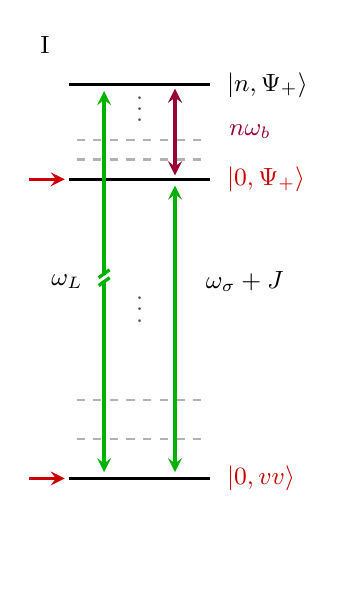
\begin{tikzpicture}[>=stealth, thick, font=\small, baseline=(current bounding box.north)]
					\def\wMain{0.9}
					\def\wFon{0.8}
					\def\yGnd{0.0}
					\def\yExc{3.8}
					\def\yTop{5.0}
					\def\yFon{2.0}
					
					% Nivel base |0,vv⟩
					\draw[black, very thick] (-\wMain, \yGnd) -- (\wMain, \yGnd);
					\node[right] at (\wMain+0.08, \yGnd) [red!80!black] {$|0,vv\rangle$};
					\draw[->, red!80!black, very thick]
					(-\wMain-0.5, \yGnd) -- (-\wMain-0.05, \yGnd);
					
					% Niveles fonónicos arriba
					\foreach \k in {1,2}{
						\pgfmathsetmacro{\yy}{\yGnd + \k*0.5}
						\draw[gray!60, dashed, thick] (-\wFon,\yy) -- (\wFon,\yy);
					}
					\node[black!70] at (0, \yGnd + 2.25) {$\vdots$};
					
					% Nivel |0,Ψ+⟩
					\draw[black, very thick] (-\wMain, \yExc) -- (\wMain, \yExc);
					\node[right] at (\wMain+0.08, \yExc) [red!80!black]  {$|0,\Psi_+\rangle$};
					\draw[->, red!80!black, very thick]
					(-\wMain-0.5, \yExc) -- (-\wMain-0.05, \yExc);
					
					% Niveles fonónicos encima de |0,\Psi+⟩
					\foreach \k in {1,2}{
						\pgfmathsetmacro{\yy}{\yExc + 0.25 + (\k-1)*0.25}
						\draw[gray!60, dashed, thick] (-\wFon,\yy) -- (\wFon,\yy);
					}
					\pgfmathsetmacro{\yvdots}{\yTop - 0.2}
					\node[black!70] at (0,\yvdots) {$\vdots$};
					
					% Nivel |n,Ψ+⟩
					\draw[black, very thick] (-\wMain, \yTop) -- (\wMain, \yTop);
					\node[right] at (\wMain+0.08, \yTop) {$|n,\Psi_+\rangle$};
					
					% Flecha nω_b
					\draw[<->, purple!80!black, very thick]
					(\wMain-0.45, \yExc+0.05) -- (\wMain-0.45, \yTop-0.05)
					node[right] at (1, {(\yExc+\yTop)/2}) {$n\omega_b$};
					
					% Flechas verdes proceso Stokes
					% Coordenada del corte
					\pgfmathsetmacro{\ybreak}{(\yGnd+\yTop)/2}
					% Línea inferior
					\draw[<-, green!70!black, very thick]
					(-0.45, \yGnd+0.08) -- (-0.45, \ybreak-0.01);
					% Línea superior
					\draw[->, green!70!black, very thick]
					(-0.45, \ybreak+0.09) -- (-0.45, \yTop-0.08);
					% Las dos rayitas //
					\draw[green!70!black, very thick]
					(-0.52, \ybreak-0.05) -- (-0.38, \ybreak+0.05);
					\draw[green!70!black, very thick]
					(-0.52, \ybreak+0.05) -- (-0.38, \ybreak+0.15);
					\node at (-0.45, \ybreak) [left=4pt] {$\omega_L$};
					\draw[<->, green!70!black, very thick]
					(0.45, \yExc-0.08) -- (0.45, \yGnd+0.08);
					\node at (+2.10, \ybreak) [left=4pt] {$\omega_{\sigma} + J$};
					% Espacio inferior fantasma para igualar (b): línea + label de lambda
					\path[draw=none] (0, \yGnd-0.5) -- (1.2, \yGnd-0.5);
					\node at (0.6, \yGnd-0.5) [below=2pt] {$\phantom{\lambda^2/\omega_b}$};
					
					% Etiqueta panel
					\node at (-\wMain-0.3, \yTop+0.5) {I};
					
				\end{tikzpicture}
			}
		\end{minipage}%
		\begin{minipage}[t]{0.325\textwidth}
			\centering
			\resizebox{\textwidth}{!}{%
				\begin{tikzpicture}[>=stealth, thick, font=\small, baseline=(current bounding box.north)]
					
					\def\wMain{0.9}
					\def\wFon{0.8}
					\def\yGnd{0.0}
					\def\yExc{4.6}
					\def\yTop{5.8}
					\def\dx{1.2}
					\def\dy{0}  % El estado base |0,vv⟩ no se mueve
					\def\dyExc{-0.6}  % Solo los estados excitados se desplazan
					\def\xlabel{\wMain+\dx+0.08}
					\def\xlabelBase{\dx+0.12}
					
					% ── BASE (no se mueve) ─────────────────────────────────────────────
					\draw[black, very thick] (-\wMain, \yGnd) -- (\wMain, \yGnd);
					\node[right] at (\xlabelBase, \yGnd) [red!80!black] {$|0,vv\rangle$};
					
					\draw[->, red!80!black, very thick]
					(-\wMain-0.5, \yGnd) -- (-\wMain-0.05, \yGnd);
					
					\foreach \k in {1,2}{
						\pgfmathsetmacro{\yy}{\yGnd + \k*0.5}
						\draw[gray!60, dashed, thick] (-\wFon,\yy) -- (\wFon,\yy);
					}
					\node[black!70] at (0.2, \yGnd+1.5) {$\vdots$};
					
					% ── COLUMNA SUPERIOR (con desplazamiento dx y dy) ──────────────────
					\draw[black, very thick] (-\wMain+\dx, \yExc+\dyExc) -- (\wMain+\dx, \yExc+\dyExc);
					\node[right] at (\wMain+\dx+0.08, \yExc+\dyExc) [red!80!black]
					{$|\widetilde{0},\Psi_+\rangle$};
					
					\draw[->, red!80!black, very thick]
					(-\wMain+\dx-0.5, \yExc+\dyExc) -- (-\wMain+\dx-0.05, \yExc+\dyExc);
					
					\foreach \k in {1,2}{
						\pgfmathsetmacro{\yy}{\yExc+\dyExc + 0.25 + (\k-1)*0.25}
						\draw[gray!60, dashed, thick] (-\wFon+\dx,\yy) -- (\wFon+\dx,\yy);
					}
					
					\pgfmathsetmacro{\yvdots}{\yTop+\dyExc-0.2}
					\node[black!70] at (\dx, \yvdots) {$\vdots$};
					
					\draw[black, very thick] (-\wMain+\dx, \yTop+\dyExc) -- (\wMain+\dx, \yTop+\dyExc);
					\node[right] at (\xlabel, \yTop+\dyExc)
					{$|\widetilde{n},\Psi_+\rangle$};
					
					% ── nω_b ───────────────────────────────────────────────────────────
					\draw[<->, purple!80!black, very thick]
					(\wMain+\dx-0.45, \yExc+\dyExc+0.05) --
					(\wMain+\dx-0.45, \yTop+\dyExc-0.05)
					node[right] at (\wMain+\dx+0.05, {(\yExc+\yTop)/2+\dyExc})
					{$n\omega_b$};
					
					% ── Desplazamiento λ²/ω_b ──────────────────────────────────────────
					\draw[<->, black!60, thick]
					(0, \yGnd-0.5) -- (\dx, \yGnd-0.5)
					node[midway, below=2pt] {$\lambda^2/\omega_b$};
					
					\draw[black!60, dashed, thick]
					(\dx, \yGnd-0.5+0.08) -- (\dx, \yExc+\dyExc-0.08);
					
					% ── ω_L con corte // ───────────────────────────────────────────────
					
					% Punto central (solo para las rayitas y label)
					\coordinate (C) at ($(-0.45, \yGnd+0.08)!0.5!(-0.45+\dx, \yTop+\dyExc-0.08)$);
					
					% Dos puntos separados para crear el corte real
					\coordinate (C1) at ($(-0.45, \yGnd+0.08)!0.50!(-0.45+\dx, \yTop+\dyExc-0.08)$);
					\coordinate (C2) at ($(-0.45, \yGnd+0.08)!0.53!(-0.45+\dx, \yTop+\dyExc-0.08)$);
					
					% Línea inferior
					\draw[green!70!black, very thick, <-]
					(-0.45, \yGnd+0.08) -- (C1);
					
					% Línea superior
					\draw[green!70!black, very thick, ->]
					(C2) -- (-0.45+\dx, \yTop+\dyExc-0.08);
					
					% Rayitas //
					\draw[green!70!black, very thick]
					($(C)+(-0.06,-0.05)$) -- ($(C)+(0.08,0.05)$);
					
					\draw[green!70!black, very thick]
					($(C)+(-0.06,0.05)$) -- ($(C)+(0.08,0.15)$);
					
					% Label
					\node[left=2pt] at (C) {$\omega_L$};
					
					% ── Emisión ────────────────────────────────────────────────────────
					\draw[<->, green!70!black, very thick, bend left=25]
					(0.45+\dx, \yExc+\dyExc-0.08) to (0.45, \yGnd+0.08);
					\node[anchor=west, text=black] at ($(C)+(1.75,0)$) {$\widetilde{\omega}_{\sigma}$};
					
					% ── Panel label ────────────────────────────────────────────────────
					\node at (-\wMain-0.3, \yTop+\dyExc+0.5) {II};
					
				\end{tikzpicture}
			}
		\end{minipage}%
		\begin{minipage}[t]{0.40\textwidth}
			\centering
			\resizebox{\textwidth}{!}{%
				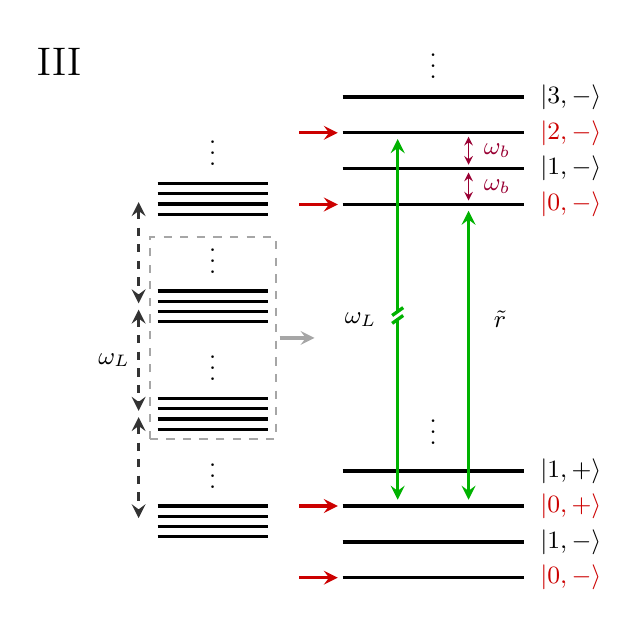
\begin{tikzpicture}[>=stealth, thick, font=\small, baseline=(current bounding box.north)]
					
					\def\xL{-1.40}
					\def\xR{1.40}
					\def\wV{0.70}
					\def\wR{1.15}
					\def\xDashed{-2.55}
					\def\xBoxL{-2.60}
					\def\xBoxR{-0.65}
					\def\xGreenOffset{0.95}
					
					\def\yGnd{0.00}
					\pgfmathsetmacro{\yOneMb}{\yGnd + 0.455}
					\pgfmathsetmacro{\yZeroP}{\yGnd + 0.910}
					\pgfmathsetmacro{\yOneP}{\yGnd + 1.356}
					\pgfmathsetmacro{\yTwoP}{\yGnd + 2.25}
					\pgfmathsetmacro{\yZeroM}{\yGnd + 4.74}
					\pgfmathsetmacro{\yOneM}{\yZeroM + 0.455}
					\pgfmathsetmacro{\yTwoM}{\yZeroM + 0.910}
					\pgfmathsetmacro{\yThreeM}{\yZeroM + 1.365}
					\def\xLPivot{\xL}
					\def\yLPivot{3.05}
					\def\sL{0.65}
					
					% ── Columna izquierda: ladder fonónico + ventana punteada ───────────
					\foreach \yy in {1.4,1.2,1.0,0.8}{
						\draw[black, very thick] (\xL-\wV,{\yy*\sL}) -- (\xL+\wV,{\yy*\sL});
					}
					\node at (\xL,{2.15*\sL}) {$\vdots$};
					
					\foreach \yy in {3.5,3.3,3.1,2.9}{
						\draw[black, very thick] (\xL-\wV,{\yy*\sL}) -- (\xL+\wV,{\yy*\sL});
					}
					\node at (\xL,{4.25*\sL}) {$\vdots$};
					
					\foreach \yy in {5.6,5.4,5.2,5.0}{
						\draw[black, very thick] (\xL-\wV,{\yy*\sL}) -- (\xL+\wV,{\yy*\sL});
					}
					\node at (\xL,{6.35*\sL}) {$\vdots$};
					
					\foreach \yy in {7.7,7.5,7.3,7.1}{
						\draw[black, very thick] (\xL-\wV,{\yy*\sL}) -- (\xL+\wV,{\yy*\sL});
					}
					\node at (\xL,{8.45*\sL}) {$\vdots$};
					
					\draw[gray!70, dashed, thick] (\xL-\wV-0.1,{3.25*\sL-0.35}) rectangle (\xL+\wV+0.1,{6.35*\sL+0.20});
					\def\gap{0.04}
					\draw[black!80, dashed, very thick, <->] (\xL-\wV-0.24,{3.2*\sL-\gap}) -- (\xL-\wV-0.24,{1.1*\sL+\gap});
					\draw[black!80, dashed, very thick, <->] (\xL-\wV-0.24,{5.3*\sL-\gap}) -- (\xL-\wV-0.24,{3.2*\sL+\gap});
					\draw[black!80, dashed, very thick, <->] (\xL-\wV-0.24,{7.4*\sL-\gap}) -- (\xL-\wV-0.24,{5.3*\sL+\gap});
					\node[left=2pt] at (\xL-\wV-0.15,{4.25*\sL}) {$\omega_L$};
					
					\draw[gray!70, very thick, ->] (\xBoxR+0.10, {(3.25*\sL-0.35 + 6.35*\sL+0.20)/2}) -- (\xBoxR+0.02+0.525, {(3.25*\sL-0.35 + 6.35*\sL+0.20)/2});
					
					% ── Columna derecha: niveles dressed ────────────────────────────────
					\draw[black, very thick] (\xR-\wR,\yThreeM) -- (\xR+\wR,\yThreeM);
					\draw[black, very thick] (\xR-\wR,\yTwoM) -- (\xR+\wR,\yTwoM);
					\draw[black, very thick] (\xR-\wR,\yOneM) -- (\xR+\wR,\yOneM);
					\draw[black, very thick] (\xR-\wR,\yZeroM) -- (\xR+\wR,\yZeroM);
					\node[black] at (\xR,\yTwoP-0.3) {$\vdots$};
					\node[black] at (\xR,\yThreeM+0.5) {$\vdots$};
					\draw[black, very thick] (\xR-\wR,\yOneP) -- (\xR+\wR,\yOneP);
					\draw[black, very thick] (\xR-\wR,\yZeroP) -- (\xR+\wR,\yZeroP);
					\draw[black, very thick] (\xR-\wR,\yOneMb) -- (\xR+\wR,\yOneMb);
					\draw[black, very thick] (\xR-\wR,\yGnd) -- (\xR+\wR,\yGnd);
					\node[right] at (\xR+\wR+0.08,\yThreeM) {$|3,-\rangle$};
					\node[right, red!80!black] at (\xR+\wR+0.08,\yTwoM) {$|2,-\rangle$};
					\node[right] at (\xR+\wR+0.08,\yOneM) {$|1,-\rangle$};
					\node[right, red!80!black] at (\xR+\wR+0.08,\yZeroM) {$|0,-\rangle$};
					\node[right] at (\xR+\wR+0.08,\yOneP) {$|1,+\rangle$};
					\node[right, red!80!black] at (\xR+\wR+0.08,\yZeroP) {$|0,+\rangle$};
					\node[right] at (\xR+\wR+0.08,\yOneMb) {$|1,-\rangle$};
					\node[right, red!80!black] at (\xR+\wR+0.08,\yGnd) {$|0,-\rangle$};
					
					\foreach \yy in {\yTwoM,\yZeroM,\yZeroP,\yGnd}{
						\draw[->, red!80!black, very thick] (\xR-\wR-0.55,\yy) -- (\xR-\wR-0.06,\yy);
					}
					
					% ── Flecha izquierda: ω_L con corte // ─────────────────────────────
					\pgfmathsetmacro{\ybreakC}{(\yZeroP+\yTwoM)/2}
					\draw[<-, green!70!black, very thick]
					(\xR-0.45, \yZeroP+0.08) -- (\xR-0.45, \ybreakC-0.01);
					\draw[->, green!70!black, very thick]
					(\xR-0.45, \ybreakC+0.09) -- (\xR-0.45, \yTwoM-0.08);
					\draw[green!70!black, very thick]
					(\xR-0.52, \ybreakC-0.05) -- (\xR-0.38, \ybreakC+0.05);
					\draw[green!70!black, very thick]
					(\xR-0.52, \ybreakC+0.05) -- (\xR-0.38, \ybreakC+0.15);
					\node[left=4pt] at (\xR-0.45, \ybreakC) {$\omega_L$};
					\node[left=4pt] at (\xR+1.20, \ybreakC) {$\tilde{r}$};
					
					\draw[<->, green!70!black, very thick]
					(\xR+0.45, \yZeroM-0.08) -- (\xR+0.45, \yZeroP+0.08);
					
					\draw[<->, purple!80!black, thin]
					(\xR+0.45, \yZeroM+0.05) -- (\xR+0.45, \yOneM-0.05)
					node[right=2pt, midway] {$\omega_b$};
					\draw[<->, purple!80!black, thin]
					(\xR+0.45, \yOneM+0.05) -- (\xR+0.45, \yTwoM-0.05)
					node[right=2pt, midway] {$\omega_b$};
					
					% Etiqueta panel
					\node at (\xBoxL-0.75,\yThreeM+0.45) {\fontsize{14}{16}\selectfont III};
					
				\end{tikzpicture}
			}
		\end{minipage}
	\end{figure}
	
\end{frame}

\section{Resultados y discusión}

\begin{frame}{Oscilaciones de Rabi}
	\vspace{-20pt}
	Un TLS conducido coherentemente oscila entre
	$|g\rangle$ y $|e\rangle$ con probabilidad
	\begin{equation*}
		P_e(t) = \frac{\Omega^2}{\Omega_R^2}
		\sin^2\!\left(\frac{\Omega_R\, t}{2}\right),
		\qquad
		\Omega_R = \sqrt{\Omega^2 + \Delta^2}.
	\end{equation*}
	
	\vspace{10pt}
	\begin{center}
		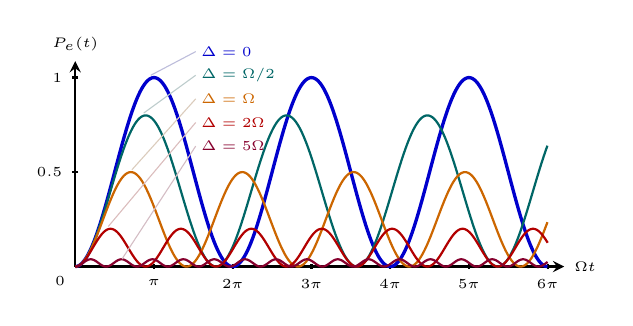
\begin{tikzpicture}[>=stealth, thick, font=\tiny, scale=0.60]
			
			\def\W{10}
			\def\H{4}
			\def\xmax{6.0}
			
			\draw[->] (0,0) -- (\W+0.35, 0) node[right] {$\Omega t$};
			\draw[->] (0,0) -- (0, \H+0.35) node[above] {$P_e(t)$};
			
			\pgfmathsetmacro{\sx}{\W/\xmax}
			\pgfmathsetmacro{\sy}{\H}
			
			\foreach \k in {1,2,3,4,5,6}{
				\pgfmathsetmacro{\xpos}{\k*\sx}
				\draw (\xpos, 0.06) -- (\xpos, -0.06);
				\ifnum\k=1
				\node[below] at (\xpos, -0.06) {$\pi$};
				\else
				\node[below] at (\xpos, -0.06) {$\k\pi$};
				\fi
			}
			\node[below left] at (0,0) {$0$};
			
			\foreach \yv/\lbl in {0.5/0.5, 1/1}{
				\draw (0.06, \yv*\sy) -- (-0.06, \yv*\sy);
				\node[left] at (-0.06, \yv*\sy) {$\lbl$};
			}
			
			\draw[blue!80!black, very thick, domain=0:\xmax, samples=400, smooth]
			plot ({\x*\sx}, {\sy * sin(90*1.0000*\x)*sin(90*1.0000*\x)});
			\draw[blue!30!gray!40, thin] (1.6000, 4.0500) -- (2.5500, 4.5500);
			\node[right, blue!80!black] at (2.4500, 4.5500) {$\Delta=0$};
			
			\draw[teal!80!black, thick, domain=0:\xmax, samples=400, smooth]
			plot ({\x*\sx}, {\sy * 0.8000 * sin(90*1.1180*\x)*sin(90*1.1180*\x)});
			\draw[teal!30!gray!40, thin] (1.4500, 3.2500) -- (2.5500, 4.0500);
			\node[right, teal!80!black] at (2.4500, 4.0500) {$\Delta=\Omega/2$};
			
			\draw[orange!80!black, thick, domain=0:\xmax, samples=400, smooth]
			plot ({\x*\sx}, {\sy * 0.5000 * sin(90*1.4142*\x)*sin(90*1.4142*\x)});
			\draw[orange!30!gray!40, thin] (1.2000, 2.0500) -- (2.5500, 3.5500);
			\node[right, orange!80!black] at (2.4500, 3.5500) {$\Delta=\Omega$};
			
			\draw[red!70!black, thick, domain=0:\xmax, samples=500, smooth]
			plot ({\x*\sx}, {\sy * 0.2000 * sin(90*2.2361*\x)*sin(90*2.2361*\x)});
			\draw[red!30!gray!40, thin] (0.7000, 0.8500) -- (2.5500, 3.0500);
			\node[right, red!70!black] at (2.4500, 3.0500) {$\Delta=2\Omega$};
			
			\draw[purple!70!black, thick, domain=0:\xmax, samples=800, smooth]
			plot ({\x*\sx}, {\sy * 0.0385 * sin(90*5.0990*\x)*sin(90*5.0990*\x)});
			\draw[purple!30!gray!40, thin] (0.9900, 0.1600) -- (2.5500, 2.5500);
			\node[right, purple!70!black] at (2.4500, 2.5500) {$\Delta=5\Omega$};
			
		\end{tikzpicture}
	\end{center}
	
	\vspace{20pt}
	{\small
		En resonancia ($\Delta=0$) la inversión es completa. Fuera de resonancia, la amplitud se suprime como $(\Omega/\Delta)^2$ y el periodo se acorta. La desintonía $\Delta$ \textbf{selecciona} qué estados intercambian energía coherentemente.}
	
\end{frame}

\begin{frame}{Oscilaciones super-Rabi}
	
	\vspace{-15pt}
	
	\begin{center}
		\resizebox{0.70\textwidth}{!}{%
			%% Creator: Matplotlib, PGF backend
%%
%% To include the figure in your LaTeX document, write
%%   \input{<filename>.pgf}
%%
%% Make sure the required packages are loaded in your preamble
%%   \usepackage{pgf}
%%
%% Also ensure that all the required font packages are loaded; for instance,
%% the lmodern package is sometimes necessary when using math font.
%%   \usepackage{lmodern}
%%
%% Figures using additional raster images can only be included by \input if
%% they are in the same directory as the main LaTeX file. For loading figures
%% from other directories you can use the `import` package
%%   \usepackage{import}
%%
%% and then include the figures with
%%   \import{<path to file>}{<filename>.pgf}
%%
%% Matplotlib used the following preamble
%%   \def\mathdefault#1{#1}
%%   \everymath=\expandafter{\the\everymath\displaystyle}
%%   \IfFileExists{scrextend.sty}{
%%     \usepackage[fontsize=12.000000pt]{scrextend}
%%   }{
%%     \renewcommand{\normalsize}{\fontsize{12.000000}{14.400000}\selectfont}
%%     \normalsize
%%   }
%%   
%%   \makeatletter\@ifpackageloaded{underscore}{}{\usepackage[strings]{underscore}}\makeatother
%%
\begingroup%
\makeatletter%
\begin{pgfpicture}%
\pgfpathrectangle{\pgfpointorigin}{\pgfqpoint{6.300000in}{4.000000in}}%
\pgfusepath{use as bounding box, clip}%
\begin{pgfscope}%
\pgfsetbuttcap%
\pgfsetmiterjoin%
\definecolor{currentfill}{rgb}{1.000000,1.000000,1.000000}%
\pgfsetfillcolor{currentfill}%
\pgfsetlinewidth{0.000000pt}%
\definecolor{currentstroke}{rgb}{1.000000,1.000000,1.000000}%
\pgfsetstrokecolor{currentstroke}%
\pgfsetdash{}{0pt}%
\pgfpathmoveto{\pgfqpoint{0.000000in}{0.000000in}}%
\pgfpathlineto{\pgfqpoint{6.300000in}{0.000000in}}%
\pgfpathlineto{\pgfqpoint{6.300000in}{4.000000in}}%
\pgfpathlineto{\pgfqpoint{0.000000in}{4.000000in}}%
\pgfpathlineto{\pgfqpoint{0.000000in}{0.000000in}}%
\pgfpathclose%
\pgfusepath{fill}%
\end{pgfscope}%
\begin{pgfscope}%
\pgfsetbuttcap%
\pgfsetmiterjoin%
\definecolor{currentfill}{rgb}{1.000000,1.000000,1.000000}%
\pgfsetfillcolor{currentfill}%
\pgfsetlinewidth{0.000000pt}%
\definecolor{currentstroke}{rgb}{0.000000,0.000000,0.000000}%
\pgfsetstrokecolor{currentstroke}%
\pgfsetstrokeopacity{0.000000}%
\pgfsetdash{}{0pt}%
\pgfpathmoveto{\pgfqpoint{0.599560in}{2.818072in}}%
\pgfpathlineto{\pgfqpoint{6.120000in}{2.818072in}}%
\pgfpathlineto{\pgfqpoint{6.120000in}{3.767193in}}%
\pgfpathlineto{\pgfqpoint{0.599560in}{3.767193in}}%
\pgfpathlineto{\pgfqpoint{0.599560in}{2.818072in}}%
\pgfpathclose%
\pgfusepath{fill}%
\end{pgfscope}%
\begin{pgfscope}%
\pgfsetbuttcap%
\pgfsetroundjoin%
\definecolor{currentfill}{rgb}{0.000000,0.000000,0.000000}%
\pgfsetfillcolor{currentfill}%
\pgfsetlinewidth{0.803000pt}%
\definecolor{currentstroke}{rgb}{0.000000,0.000000,0.000000}%
\pgfsetstrokecolor{currentstroke}%
\pgfsetdash{}{0pt}%
\pgfsys@defobject{currentmarker}{\pgfqpoint{0.000000in}{-0.048611in}}{\pgfqpoint{0.000000in}{0.000000in}}{%
\pgfpathmoveto{\pgfqpoint{0.000000in}{0.000000in}}%
\pgfpathlineto{\pgfqpoint{0.000000in}{-0.048611in}}%
\pgfusepath{stroke,fill}%
}%
\begin{pgfscope}%
\pgfsys@transformshift{1.738947in}{2.818072in}%
\pgfsys@useobject{currentmarker}{}%
\end{pgfscope}%
\end{pgfscope}%
\begin{pgfscope}%
\pgfsetbuttcap%
\pgfsetroundjoin%
\definecolor{currentfill}{rgb}{0.000000,0.000000,0.000000}%
\pgfsetfillcolor{currentfill}%
\pgfsetlinewidth{0.803000pt}%
\definecolor{currentstroke}{rgb}{0.000000,0.000000,0.000000}%
\pgfsetstrokecolor{currentstroke}%
\pgfsetdash{}{0pt}%
\pgfsys@defobject{currentmarker}{\pgfqpoint{0.000000in}{-0.048611in}}{\pgfqpoint{0.000000in}{0.000000in}}{%
\pgfpathmoveto{\pgfqpoint{0.000000in}{0.000000in}}%
\pgfpathlineto{\pgfqpoint{0.000000in}{-0.048611in}}%
\pgfusepath{stroke,fill}%
}%
\begin{pgfscope}%
\pgfsys@transformshift{5.157107in}{2.818072in}%
\pgfsys@useobject{currentmarker}{}%
\end{pgfscope}%
\end{pgfscope}%
\begin{pgfscope}%
\pgfsetbuttcap%
\pgfsetroundjoin%
\definecolor{currentfill}{rgb}{0.000000,0.000000,0.000000}%
\pgfsetfillcolor{currentfill}%
\pgfsetlinewidth{0.602250pt}%
\definecolor{currentstroke}{rgb}{0.000000,0.000000,0.000000}%
\pgfsetstrokecolor{currentstroke}%
\pgfsetdash{}{0pt}%
\pgfsys@defobject{currentmarker}{\pgfqpoint{0.000000in}{-0.027778in}}{\pgfqpoint{0.000000in}{0.000000in}}{%
\pgfpathmoveto{\pgfqpoint{0.000000in}{0.000000in}}%
\pgfpathlineto{\pgfqpoint{0.000000in}{-0.027778in}}%
\pgfusepath{stroke,fill}%
}%
\begin{pgfscope}%
\pgfsys@transformshift{0.942550in}{2.818072in}%
\pgfsys@useobject{currentmarker}{}%
\end{pgfscope}%
\end{pgfscope}%
\begin{pgfscope}%
\pgfsetbuttcap%
\pgfsetroundjoin%
\definecolor{currentfill}{rgb}{0.000000,0.000000,0.000000}%
\pgfsetfillcolor{currentfill}%
\pgfsetlinewidth{0.602250pt}%
\definecolor{currentstroke}{rgb}{0.000000,0.000000,0.000000}%
\pgfsetstrokecolor{currentstroke}%
\pgfsetdash{}{0pt}%
\pgfsys@defobject{currentmarker}{\pgfqpoint{0.000000in}{-0.027778in}}{\pgfqpoint{0.000000in}{0.000000in}}{%
\pgfpathmoveto{\pgfqpoint{0.000000in}{0.000000in}}%
\pgfpathlineto{\pgfqpoint{0.000000in}{-0.027778in}}%
\pgfusepath{stroke,fill}%
}%
\begin{pgfscope}%
\pgfsys@transformshift{1.143186in}{2.818072in}%
\pgfsys@useobject{currentmarker}{}%
\end{pgfscope}%
\end{pgfscope}%
\begin{pgfscope}%
\pgfsetbuttcap%
\pgfsetroundjoin%
\definecolor{currentfill}{rgb}{0.000000,0.000000,0.000000}%
\pgfsetfillcolor{currentfill}%
\pgfsetlinewidth{0.602250pt}%
\definecolor{currentstroke}{rgb}{0.000000,0.000000,0.000000}%
\pgfsetstrokecolor{currentstroke}%
\pgfsetdash{}{0pt}%
\pgfsys@defobject{currentmarker}{\pgfqpoint{0.000000in}{-0.027778in}}{\pgfqpoint{0.000000in}{0.000000in}}{%
\pgfpathmoveto{\pgfqpoint{0.000000in}{0.000000in}}%
\pgfpathlineto{\pgfqpoint{0.000000in}{-0.027778in}}%
\pgfusepath{stroke,fill}%
}%
\begin{pgfscope}%
\pgfsys@transformshift{1.285539in}{2.818072in}%
\pgfsys@useobject{currentmarker}{}%
\end{pgfscope}%
\end{pgfscope}%
\begin{pgfscope}%
\pgfsetbuttcap%
\pgfsetroundjoin%
\definecolor{currentfill}{rgb}{0.000000,0.000000,0.000000}%
\pgfsetfillcolor{currentfill}%
\pgfsetlinewidth{0.602250pt}%
\definecolor{currentstroke}{rgb}{0.000000,0.000000,0.000000}%
\pgfsetstrokecolor{currentstroke}%
\pgfsetdash{}{0pt}%
\pgfsys@defobject{currentmarker}{\pgfqpoint{0.000000in}{-0.027778in}}{\pgfqpoint{0.000000in}{0.000000in}}{%
\pgfpathmoveto{\pgfqpoint{0.000000in}{0.000000in}}%
\pgfpathlineto{\pgfqpoint{0.000000in}{-0.027778in}}%
\pgfusepath{stroke,fill}%
}%
\begin{pgfscope}%
\pgfsys@transformshift{1.395957in}{2.818072in}%
\pgfsys@useobject{currentmarker}{}%
\end{pgfscope}%
\end{pgfscope}%
\begin{pgfscope}%
\pgfsetbuttcap%
\pgfsetroundjoin%
\definecolor{currentfill}{rgb}{0.000000,0.000000,0.000000}%
\pgfsetfillcolor{currentfill}%
\pgfsetlinewidth{0.602250pt}%
\definecolor{currentstroke}{rgb}{0.000000,0.000000,0.000000}%
\pgfsetstrokecolor{currentstroke}%
\pgfsetdash{}{0pt}%
\pgfsys@defobject{currentmarker}{\pgfqpoint{0.000000in}{-0.027778in}}{\pgfqpoint{0.000000in}{0.000000in}}{%
\pgfpathmoveto{\pgfqpoint{0.000000in}{0.000000in}}%
\pgfpathlineto{\pgfqpoint{0.000000in}{-0.027778in}}%
\pgfusepath{stroke,fill}%
}%
\begin{pgfscope}%
\pgfsys@transformshift{1.486175in}{2.818072in}%
\pgfsys@useobject{currentmarker}{}%
\end{pgfscope}%
\end{pgfscope}%
\begin{pgfscope}%
\pgfsetbuttcap%
\pgfsetroundjoin%
\definecolor{currentfill}{rgb}{0.000000,0.000000,0.000000}%
\pgfsetfillcolor{currentfill}%
\pgfsetlinewidth{0.602250pt}%
\definecolor{currentstroke}{rgb}{0.000000,0.000000,0.000000}%
\pgfsetstrokecolor{currentstroke}%
\pgfsetdash{}{0pt}%
\pgfsys@defobject{currentmarker}{\pgfqpoint{0.000000in}{-0.027778in}}{\pgfqpoint{0.000000in}{0.000000in}}{%
\pgfpathmoveto{\pgfqpoint{0.000000in}{0.000000in}}%
\pgfpathlineto{\pgfqpoint{0.000000in}{-0.027778in}}%
\pgfusepath{stroke,fill}%
}%
\begin{pgfscope}%
\pgfsys@transformshift{1.562454in}{2.818072in}%
\pgfsys@useobject{currentmarker}{}%
\end{pgfscope}%
\end{pgfscope}%
\begin{pgfscope}%
\pgfsetbuttcap%
\pgfsetroundjoin%
\definecolor{currentfill}{rgb}{0.000000,0.000000,0.000000}%
\pgfsetfillcolor{currentfill}%
\pgfsetlinewidth{0.602250pt}%
\definecolor{currentstroke}{rgb}{0.000000,0.000000,0.000000}%
\pgfsetstrokecolor{currentstroke}%
\pgfsetdash{}{0pt}%
\pgfsys@defobject{currentmarker}{\pgfqpoint{0.000000in}{-0.027778in}}{\pgfqpoint{0.000000in}{0.000000in}}{%
\pgfpathmoveto{\pgfqpoint{0.000000in}{0.000000in}}%
\pgfpathlineto{\pgfqpoint{0.000000in}{-0.027778in}}%
\pgfusepath{stroke,fill}%
}%
\begin{pgfscope}%
\pgfsys@transformshift{1.628529in}{2.818072in}%
\pgfsys@useobject{currentmarker}{}%
\end{pgfscope}%
\end{pgfscope}%
\begin{pgfscope}%
\pgfsetbuttcap%
\pgfsetroundjoin%
\definecolor{currentfill}{rgb}{0.000000,0.000000,0.000000}%
\pgfsetfillcolor{currentfill}%
\pgfsetlinewidth{0.602250pt}%
\definecolor{currentstroke}{rgb}{0.000000,0.000000,0.000000}%
\pgfsetstrokecolor{currentstroke}%
\pgfsetdash{}{0pt}%
\pgfsys@defobject{currentmarker}{\pgfqpoint{0.000000in}{-0.027778in}}{\pgfqpoint{0.000000in}{0.000000in}}{%
\pgfpathmoveto{\pgfqpoint{0.000000in}{0.000000in}}%
\pgfpathlineto{\pgfqpoint{0.000000in}{-0.027778in}}%
\pgfusepath{stroke,fill}%
}%
\begin{pgfscope}%
\pgfsys@transformshift{1.686811in}{2.818072in}%
\pgfsys@useobject{currentmarker}{}%
\end{pgfscope}%
\end{pgfscope}%
\begin{pgfscope}%
\pgfsetbuttcap%
\pgfsetroundjoin%
\definecolor{currentfill}{rgb}{0.000000,0.000000,0.000000}%
\pgfsetfillcolor{currentfill}%
\pgfsetlinewidth{0.602250pt}%
\definecolor{currentstroke}{rgb}{0.000000,0.000000,0.000000}%
\pgfsetstrokecolor{currentstroke}%
\pgfsetdash{}{0pt}%
\pgfsys@defobject{currentmarker}{\pgfqpoint{0.000000in}{-0.027778in}}{\pgfqpoint{0.000000in}{0.000000in}}{%
\pgfpathmoveto{\pgfqpoint{0.000000in}{0.000000in}}%
\pgfpathlineto{\pgfqpoint{0.000000in}{-0.027778in}}%
\pgfusepath{stroke,fill}%
}%
\begin{pgfscope}%
\pgfsys@transformshift{2.081936in}{2.818072in}%
\pgfsys@useobject{currentmarker}{}%
\end{pgfscope}%
\end{pgfscope}%
\begin{pgfscope}%
\pgfsetbuttcap%
\pgfsetroundjoin%
\definecolor{currentfill}{rgb}{0.000000,0.000000,0.000000}%
\pgfsetfillcolor{currentfill}%
\pgfsetlinewidth{0.602250pt}%
\definecolor{currentstroke}{rgb}{0.000000,0.000000,0.000000}%
\pgfsetstrokecolor{currentstroke}%
\pgfsetdash{}{0pt}%
\pgfsys@defobject{currentmarker}{\pgfqpoint{0.000000in}{-0.027778in}}{\pgfqpoint{0.000000in}{0.000000in}}{%
\pgfpathmoveto{\pgfqpoint{0.000000in}{0.000000in}}%
\pgfpathlineto{\pgfqpoint{0.000000in}{-0.027778in}}%
\pgfusepath{stroke,fill}%
}%
\begin{pgfscope}%
\pgfsys@transformshift{2.282572in}{2.818072in}%
\pgfsys@useobject{currentmarker}{}%
\end{pgfscope}%
\end{pgfscope}%
\begin{pgfscope}%
\pgfsetbuttcap%
\pgfsetroundjoin%
\definecolor{currentfill}{rgb}{0.000000,0.000000,0.000000}%
\pgfsetfillcolor{currentfill}%
\pgfsetlinewidth{0.602250pt}%
\definecolor{currentstroke}{rgb}{0.000000,0.000000,0.000000}%
\pgfsetstrokecolor{currentstroke}%
\pgfsetdash{}{0pt}%
\pgfsys@defobject{currentmarker}{\pgfqpoint{0.000000in}{-0.027778in}}{\pgfqpoint{0.000000in}{0.000000in}}{%
\pgfpathmoveto{\pgfqpoint{0.000000in}{0.000000in}}%
\pgfpathlineto{\pgfqpoint{0.000000in}{-0.027778in}}%
\pgfusepath{stroke,fill}%
}%
\begin{pgfscope}%
\pgfsys@transformshift{2.424926in}{2.818072in}%
\pgfsys@useobject{currentmarker}{}%
\end{pgfscope}%
\end{pgfscope}%
\begin{pgfscope}%
\pgfsetbuttcap%
\pgfsetroundjoin%
\definecolor{currentfill}{rgb}{0.000000,0.000000,0.000000}%
\pgfsetfillcolor{currentfill}%
\pgfsetlinewidth{0.602250pt}%
\definecolor{currentstroke}{rgb}{0.000000,0.000000,0.000000}%
\pgfsetstrokecolor{currentstroke}%
\pgfsetdash{}{0pt}%
\pgfsys@defobject{currentmarker}{\pgfqpoint{0.000000in}{-0.027778in}}{\pgfqpoint{0.000000in}{0.000000in}}{%
\pgfpathmoveto{\pgfqpoint{0.000000in}{0.000000in}}%
\pgfpathlineto{\pgfqpoint{0.000000in}{-0.027778in}}%
\pgfusepath{stroke,fill}%
}%
\begin{pgfscope}%
\pgfsys@transformshift{2.535344in}{2.818072in}%
\pgfsys@useobject{currentmarker}{}%
\end{pgfscope}%
\end{pgfscope}%
\begin{pgfscope}%
\pgfsetbuttcap%
\pgfsetroundjoin%
\definecolor{currentfill}{rgb}{0.000000,0.000000,0.000000}%
\pgfsetfillcolor{currentfill}%
\pgfsetlinewidth{0.602250pt}%
\definecolor{currentstroke}{rgb}{0.000000,0.000000,0.000000}%
\pgfsetstrokecolor{currentstroke}%
\pgfsetdash{}{0pt}%
\pgfsys@defobject{currentmarker}{\pgfqpoint{0.000000in}{-0.027778in}}{\pgfqpoint{0.000000in}{0.000000in}}{%
\pgfpathmoveto{\pgfqpoint{0.000000in}{0.000000in}}%
\pgfpathlineto{\pgfqpoint{0.000000in}{-0.027778in}}%
\pgfusepath{stroke,fill}%
}%
\begin{pgfscope}%
\pgfsys@transformshift{2.625562in}{2.818072in}%
\pgfsys@useobject{currentmarker}{}%
\end{pgfscope}%
\end{pgfscope}%
\begin{pgfscope}%
\pgfsetbuttcap%
\pgfsetroundjoin%
\definecolor{currentfill}{rgb}{0.000000,0.000000,0.000000}%
\pgfsetfillcolor{currentfill}%
\pgfsetlinewidth{0.602250pt}%
\definecolor{currentstroke}{rgb}{0.000000,0.000000,0.000000}%
\pgfsetstrokecolor{currentstroke}%
\pgfsetdash{}{0pt}%
\pgfsys@defobject{currentmarker}{\pgfqpoint{0.000000in}{-0.027778in}}{\pgfqpoint{0.000000in}{0.000000in}}{%
\pgfpathmoveto{\pgfqpoint{0.000000in}{0.000000in}}%
\pgfpathlineto{\pgfqpoint{0.000000in}{-0.027778in}}%
\pgfusepath{stroke,fill}%
}%
\begin{pgfscope}%
\pgfsys@transformshift{2.701840in}{2.818072in}%
\pgfsys@useobject{currentmarker}{}%
\end{pgfscope}%
\end{pgfscope}%
\begin{pgfscope}%
\pgfsetbuttcap%
\pgfsetroundjoin%
\definecolor{currentfill}{rgb}{0.000000,0.000000,0.000000}%
\pgfsetfillcolor{currentfill}%
\pgfsetlinewidth{0.602250pt}%
\definecolor{currentstroke}{rgb}{0.000000,0.000000,0.000000}%
\pgfsetstrokecolor{currentstroke}%
\pgfsetdash{}{0pt}%
\pgfsys@defobject{currentmarker}{\pgfqpoint{0.000000in}{-0.027778in}}{\pgfqpoint{0.000000in}{0.000000in}}{%
\pgfpathmoveto{\pgfqpoint{0.000000in}{0.000000in}}%
\pgfpathlineto{\pgfqpoint{0.000000in}{-0.027778in}}%
\pgfusepath{stroke,fill}%
}%
\begin{pgfscope}%
\pgfsys@transformshift{2.767915in}{2.818072in}%
\pgfsys@useobject{currentmarker}{}%
\end{pgfscope}%
\end{pgfscope}%
\begin{pgfscope}%
\pgfsetbuttcap%
\pgfsetroundjoin%
\definecolor{currentfill}{rgb}{0.000000,0.000000,0.000000}%
\pgfsetfillcolor{currentfill}%
\pgfsetlinewidth{0.602250pt}%
\definecolor{currentstroke}{rgb}{0.000000,0.000000,0.000000}%
\pgfsetstrokecolor{currentstroke}%
\pgfsetdash{}{0pt}%
\pgfsys@defobject{currentmarker}{\pgfqpoint{0.000000in}{-0.027778in}}{\pgfqpoint{0.000000in}{0.000000in}}{%
\pgfpathmoveto{\pgfqpoint{0.000000in}{0.000000in}}%
\pgfpathlineto{\pgfqpoint{0.000000in}{-0.027778in}}%
\pgfusepath{stroke,fill}%
}%
\begin{pgfscope}%
\pgfsys@transformshift{2.826198in}{2.818072in}%
\pgfsys@useobject{currentmarker}{}%
\end{pgfscope}%
\end{pgfscope}%
\begin{pgfscope}%
\pgfsetbuttcap%
\pgfsetroundjoin%
\definecolor{currentfill}{rgb}{0.000000,0.000000,0.000000}%
\pgfsetfillcolor{currentfill}%
\pgfsetlinewidth{0.602250pt}%
\definecolor{currentstroke}{rgb}{0.000000,0.000000,0.000000}%
\pgfsetstrokecolor{currentstroke}%
\pgfsetdash{}{0pt}%
\pgfsys@defobject{currentmarker}{\pgfqpoint{0.000000in}{-0.027778in}}{\pgfqpoint{0.000000in}{0.000000in}}{%
\pgfpathmoveto{\pgfqpoint{0.000000in}{0.000000in}}%
\pgfpathlineto{\pgfqpoint{0.000000in}{-0.027778in}}%
\pgfusepath{stroke,fill}%
}%
\begin{pgfscope}%
\pgfsys@transformshift{3.221323in}{2.818072in}%
\pgfsys@useobject{currentmarker}{}%
\end{pgfscope}%
\end{pgfscope}%
\begin{pgfscope}%
\pgfsetbuttcap%
\pgfsetroundjoin%
\definecolor{currentfill}{rgb}{0.000000,0.000000,0.000000}%
\pgfsetfillcolor{currentfill}%
\pgfsetlinewidth{0.602250pt}%
\definecolor{currentstroke}{rgb}{0.000000,0.000000,0.000000}%
\pgfsetstrokecolor{currentstroke}%
\pgfsetdash{}{0pt}%
\pgfsys@defobject{currentmarker}{\pgfqpoint{0.000000in}{-0.027778in}}{\pgfqpoint{0.000000in}{0.000000in}}{%
\pgfpathmoveto{\pgfqpoint{0.000000in}{0.000000in}}%
\pgfpathlineto{\pgfqpoint{0.000000in}{-0.027778in}}%
\pgfusepath{stroke,fill}%
}%
\begin{pgfscope}%
\pgfsys@transformshift{3.421959in}{2.818072in}%
\pgfsys@useobject{currentmarker}{}%
\end{pgfscope}%
\end{pgfscope}%
\begin{pgfscope}%
\pgfsetbuttcap%
\pgfsetroundjoin%
\definecolor{currentfill}{rgb}{0.000000,0.000000,0.000000}%
\pgfsetfillcolor{currentfill}%
\pgfsetlinewidth{0.602250pt}%
\definecolor{currentstroke}{rgb}{0.000000,0.000000,0.000000}%
\pgfsetstrokecolor{currentstroke}%
\pgfsetdash{}{0pt}%
\pgfsys@defobject{currentmarker}{\pgfqpoint{0.000000in}{-0.027778in}}{\pgfqpoint{0.000000in}{0.000000in}}{%
\pgfpathmoveto{\pgfqpoint{0.000000in}{0.000000in}}%
\pgfpathlineto{\pgfqpoint{0.000000in}{-0.027778in}}%
\pgfusepath{stroke,fill}%
}%
\begin{pgfscope}%
\pgfsys@transformshift{3.564312in}{2.818072in}%
\pgfsys@useobject{currentmarker}{}%
\end{pgfscope}%
\end{pgfscope}%
\begin{pgfscope}%
\pgfsetbuttcap%
\pgfsetroundjoin%
\definecolor{currentfill}{rgb}{0.000000,0.000000,0.000000}%
\pgfsetfillcolor{currentfill}%
\pgfsetlinewidth{0.602250pt}%
\definecolor{currentstroke}{rgb}{0.000000,0.000000,0.000000}%
\pgfsetstrokecolor{currentstroke}%
\pgfsetdash{}{0pt}%
\pgfsys@defobject{currentmarker}{\pgfqpoint{0.000000in}{-0.027778in}}{\pgfqpoint{0.000000in}{0.000000in}}{%
\pgfpathmoveto{\pgfqpoint{0.000000in}{0.000000in}}%
\pgfpathlineto{\pgfqpoint{0.000000in}{-0.027778in}}%
\pgfusepath{stroke,fill}%
}%
\begin{pgfscope}%
\pgfsys@transformshift{3.674730in}{2.818072in}%
\pgfsys@useobject{currentmarker}{}%
\end{pgfscope}%
\end{pgfscope}%
\begin{pgfscope}%
\pgfsetbuttcap%
\pgfsetroundjoin%
\definecolor{currentfill}{rgb}{0.000000,0.000000,0.000000}%
\pgfsetfillcolor{currentfill}%
\pgfsetlinewidth{0.602250pt}%
\definecolor{currentstroke}{rgb}{0.000000,0.000000,0.000000}%
\pgfsetstrokecolor{currentstroke}%
\pgfsetdash{}{0pt}%
\pgfsys@defobject{currentmarker}{\pgfqpoint{0.000000in}{-0.027778in}}{\pgfqpoint{0.000000in}{0.000000in}}{%
\pgfpathmoveto{\pgfqpoint{0.000000in}{0.000000in}}%
\pgfpathlineto{\pgfqpoint{0.000000in}{-0.027778in}}%
\pgfusepath{stroke,fill}%
}%
\begin{pgfscope}%
\pgfsys@transformshift{3.764948in}{2.818072in}%
\pgfsys@useobject{currentmarker}{}%
\end{pgfscope}%
\end{pgfscope}%
\begin{pgfscope}%
\pgfsetbuttcap%
\pgfsetroundjoin%
\definecolor{currentfill}{rgb}{0.000000,0.000000,0.000000}%
\pgfsetfillcolor{currentfill}%
\pgfsetlinewidth{0.602250pt}%
\definecolor{currentstroke}{rgb}{0.000000,0.000000,0.000000}%
\pgfsetstrokecolor{currentstroke}%
\pgfsetdash{}{0pt}%
\pgfsys@defobject{currentmarker}{\pgfqpoint{0.000000in}{-0.027778in}}{\pgfqpoint{0.000000in}{0.000000in}}{%
\pgfpathmoveto{\pgfqpoint{0.000000in}{0.000000in}}%
\pgfpathlineto{\pgfqpoint{0.000000in}{-0.027778in}}%
\pgfusepath{stroke,fill}%
}%
\begin{pgfscope}%
\pgfsys@transformshift{3.841227in}{2.818072in}%
\pgfsys@useobject{currentmarker}{}%
\end{pgfscope}%
\end{pgfscope}%
\begin{pgfscope}%
\pgfsetbuttcap%
\pgfsetroundjoin%
\definecolor{currentfill}{rgb}{0.000000,0.000000,0.000000}%
\pgfsetfillcolor{currentfill}%
\pgfsetlinewidth{0.602250pt}%
\definecolor{currentstroke}{rgb}{0.000000,0.000000,0.000000}%
\pgfsetstrokecolor{currentstroke}%
\pgfsetdash{}{0pt}%
\pgfsys@defobject{currentmarker}{\pgfqpoint{0.000000in}{-0.027778in}}{\pgfqpoint{0.000000in}{0.000000in}}{%
\pgfpathmoveto{\pgfqpoint{0.000000in}{0.000000in}}%
\pgfpathlineto{\pgfqpoint{0.000000in}{-0.027778in}}%
\pgfusepath{stroke,fill}%
}%
\begin{pgfscope}%
\pgfsys@transformshift{3.907302in}{2.818072in}%
\pgfsys@useobject{currentmarker}{}%
\end{pgfscope}%
\end{pgfscope}%
\begin{pgfscope}%
\pgfsetbuttcap%
\pgfsetroundjoin%
\definecolor{currentfill}{rgb}{0.000000,0.000000,0.000000}%
\pgfsetfillcolor{currentfill}%
\pgfsetlinewidth{0.602250pt}%
\definecolor{currentstroke}{rgb}{0.000000,0.000000,0.000000}%
\pgfsetstrokecolor{currentstroke}%
\pgfsetdash{}{0pt}%
\pgfsys@defobject{currentmarker}{\pgfqpoint{0.000000in}{-0.027778in}}{\pgfqpoint{0.000000in}{0.000000in}}{%
\pgfpathmoveto{\pgfqpoint{0.000000in}{0.000000in}}%
\pgfpathlineto{\pgfqpoint{0.000000in}{-0.027778in}}%
\pgfusepath{stroke,fill}%
}%
\begin{pgfscope}%
\pgfsys@transformshift{3.965585in}{2.818072in}%
\pgfsys@useobject{currentmarker}{}%
\end{pgfscope}%
\end{pgfscope}%
\begin{pgfscope}%
\pgfsetbuttcap%
\pgfsetroundjoin%
\definecolor{currentfill}{rgb}{0.000000,0.000000,0.000000}%
\pgfsetfillcolor{currentfill}%
\pgfsetlinewidth{0.602250pt}%
\definecolor{currentstroke}{rgb}{0.000000,0.000000,0.000000}%
\pgfsetstrokecolor{currentstroke}%
\pgfsetdash{}{0pt}%
\pgfsys@defobject{currentmarker}{\pgfqpoint{0.000000in}{-0.027778in}}{\pgfqpoint{0.000000in}{0.000000in}}{%
\pgfpathmoveto{\pgfqpoint{0.000000in}{0.000000in}}%
\pgfpathlineto{\pgfqpoint{0.000000in}{-0.027778in}}%
\pgfusepath{stroke,fill}%
}%
\begin{pgfscope}%
\pgfsys@transformshift{4.360710in}{2.818072in}%
\pgfsys@useobject{currentmarker}{}%
\end{pgfscope}%
\end{pgfscope}%
\begin{pgfscope}%
\pgfsetbuttcap%
\pgfsetroundjoin%
\definecolor{currentfill}{rgb}{0.000000,0.000000,0.000000}%
\pgfsetfillcolor{currentfill}%
\pgfsetlinewidth{0.602250pt}%
\definecolor{currentstroke}{rgb}{0.000000,0.000000,0.000000}%
\pgfsetstrokecolor{currentstroke}%
\pgfsetdash{}{0pt}%
\pgfsys@defobject{currentmarker}{\pgfqpoint{0.000000in}{-0.027778in}}{\pgfqpoint{0.000000in}{0.000000in}}{%
\pgfpathmoveto{\pgfqpoint{0.000000in}{0.000000in}}%
\pgfpathlineto{\pgfqpoint{0.000000in}{-0.027778in}}%
\pgfusepath{stroke,fill}%
}%
\begin{pgfscope}%
\pgfsys@transformshift{4.561346in}{2.818072in}%
\pgfsys@useobject{currentmarker}{}%
\end{pgfscope}%
\end{pgfscope}%
\begin{pgfscope}%
\pgfsetbuttcap%
\pgfsetroundjoin%
\definecolor{currentfill}{rgb}{0.000000,0.000000,0.000000}%
\pgfsetfillcolor{currentfill}%
\pgfsetlinewidth{0.602250pt}%
\definecolor{currentstroke}{rgb}{0.000000,0.000000,0.000000}%
\pgfsetstrokecolor{currentstroke}%
\pgfsetdash{}{0pt}%
\pgfsys@defobject{currentmarker}{\pgfqpoint{0.000000in}{-0.027778in}}{\pgfqpoint{0.000000in}{0.000000in}}{%
\pgfpathmoveto{\pgfqpoint{0.000000in}{0.000000in}}%
\pgfpathlineto{\pgfqpoint{0.000000in}{-0.027778in}}%
\pgfusepath{stroke,fill}%
}%
\begin{pgfscope}%
\pgfsys@transformshift{4.703699in}{2.818072in}%
\pgfsys@useobject{currentmarker}{}%
\end{pgfscope}%
\end{pgfscope}%
\begin{pgfscope}%
\pgfsetbuttcap%
\pgfsetroundjoin%
\definecolor{currentfill}{rgb}{0.000000,0.000000,0.000000}%
\pgfsetfillcolor{currentfill}%
\pgfsetlinewidth{0.602250pt}%
\definecolor{currentstroke}{rgb}{0.000000,0.000000,0.000000}%
\pgfsetstrokecolor{currentstroke}%
\pgfsetdash{}{0pt}%
\pgfsys@defobject{currentmarker}{\pgfqpoint{0.000000in}{-0.027778in}}{\pgfqpoint{0.000000in}{0.000000in}}{%
\pgfpathmoveto{\pgfqpoint{0.000000in}{0.000000in}}%
\pgfpathlineto{\pgfqpoint{0.000000in}{-0.027778in}}%
\pgfusepath{stroke,fill}%
}%
\begin{pgfscope}%
\pgfsys@transformshift{4.814117in}{2.818072in}%
\pgfsys@useobject{currentmarker}{}%
\end{pgfscope}%
\end{pgfscope}%
\begin{pgfscope}%
\pgfsetbuttcap%
\pgfsetroundjoin%
\definecolor{currentfill}{rgb}{0.000000,0.000000,0.000000}%
\pgfsetfillcolor{currentfill}%
\pgfsetlinewidth{0.602250pt}%
\definecolor{currentstroke}{rgb}{0.000000,0.000000,0.000000}%
\pgfsetstrokecolor{currentstroke}%
\pgfsetdash{}{0pt}%
\pgfsys@defobject{currentmarker}{\pgfqpoint{0.000000in}{-0.027778in}}{\pgfqpoint{0.000000in}{0.000000in}}{%
\pgfpathmoveto{\pgfqpoint{0.000000in}{0.000000in}}%
\pgfpathlineto{\pgfqpoint{0.000000in}{-0.027778in}}%
\pgfusepath{stroke,fill}%
}%
\begin{pgfscope}%
\pgfsys@transformshift{4.904335in}{2.818072in}%
\pgfsys@useobject{currentmarker}{}%
\end{pgfscope}%
\end{pgfscope}%
\begin{pgfscope}%
\pgfsetbuttcap%
\pgfsetroundjoin%
\definecolor{currentfill}{rgb}{0.000000,0.000000,0.000000}%
\pgfsetfillcolor{currentfill}%
\pgfsetlinewidth{0.602250pt}%
\definecolor{currentstroke}{rgb}{0.000000,0.000000,0.000000}%
\pgfsetstrokecolor{currentstroke}%
\pgfsetdash{}{0pt}%
\pgfsys@defobject{currentmarker}{\pgfqpoint{0.000000in}{-0.027778in}}{\pgfqpoint{0.000000in}{0.000000in}}{%
\pgfpathmoveto{\pgfqpoint{0.000000in}{0.000000in}}%
\pgfpathlineto{\pgfqpoint{0.000000in}{-0.027778in}}%
\pgfusepath{stroke,fill}%
}%
\begin{pgfscope}%
\pgfsys@transformshift{4.980613in}{2.818072in}%
\pgfsys@useobject{currentmarker}{}%
\end{pgfscope}%
\end{pgfscope}%
\begin{pgfscope}%
\pgfsetbuttcap%
\pgfsetroundjoin%
\definecolor{currentfill}{rgb}{0.000000,0.000000,0.000000}%
\pgfsetfillcolor{currentfill}%
\pgfsetlinewidth{0.602250pt}%
\definecolor{currentstroke}{rgb}{0.000000,0.000000,0.000000}%
\pgfsetstrokecolor{currentstroke}%
\pgfsetdash{}{0pt}%
\pgfsys@defobject{currentmarker}{\pgfqpoint{0.000000in}{-0.027778in}}{\pgfqpoint{0.000000in}{0.000000in}}{%
\pgfpathmoveto{\pgfqpoint{0.000000in}{0.000000in}}%
\pgfpathlineto{\pgfqpoint{0.000000in}{-0.027778in}}%
\pgfusepath{stroke,fill}%
}%
\begin{pgfscope}%
\pgfsys@transformshift{5.046689in}{2.818072in}%
\pgfsys@useobject{currentmarker}{}%
\end{pgfscope}%
\end{pgfscope}%
\begin{pgfscope}%
\pgfsetbuttcap%
\pgfsetroundjoin%
\definecolor{currentfill}{rgb}{0.000000,0.000000,0.000000}%
\pgfsetfillcolor{currentfill}%
\pgfsetlinewidth{0.602250pt}%
\definecolor{currentstroke}{rgb}{0.000000,0.000000,0.000000}%
\pgfsetstrokecolor{currentstroke}%
\pgfsetdash{}{0pt}%
\pgfsys@defobject{currentmarker}{\pgfqpoint{0.000000in}{-0.027778in}}{\pgfqpoint{0.000000in}{0.000000in}}{%
\pgfpathmoveto{\pgfqpoint{0.000000in}{0.000000in}}%
\pgfpathlineto{\pgfqpoint{0.000000in}{-0.027778in}}%
\pgfusepath{stroke,fill}%
}%
\begin{pgfscope}%
\pgfsys@transformshift{5.104971in}{2.818072in}%
\pgfsys@useobject{currentmarker}{}%
\end{pgfscope}%
\end{pgfscope}%
\begin{pgfscope}%
\pgfsetbuttcap%
\pgfsetroundjoin%
\definecolor{currentfill}{rgb}{0.000000,0.000000,0.000000}%
\pgfsetfillcolor{currentfill}%
\pgfsetlinewidth{0.602250pt}%
\definecolor{currentstroke}{rgb}{0.000000,0.000000,0.000000}%
\pgfsetstrokecolor{currentstroke}%
\pgfsetdash{}{0pt}%
\pgfsys@defobject{currentmarker}{\pgfqpoint{0.000000in}{-0.027778in}}{\pgfqpoint{0.000000in}{0.000000in}}{%
\pgfpathmoveto{\pgfqpoint{0.000000in}{0.000000in}}%
\pgfpathlineto{\pgfqpoint{0.000000in}{-0.027778in}}%
\pgfusepath{stroke,fill}%
}%
\begin{pgfscope}%
\pgfsys@transformshift{5.500096in}{2.818072in}%
\pgfsys@useobject{currentmarker}{}%
\end{pgfscope}%
\end{pgfscope}%
\begin{pgfscope}%
\pgfsetbuttcap%
\pgfsetroundjoin%
\definecolor{currentfill}{rgb}{0.000000,0.000000,0.000000}%
\pgfsetfillcolor{currentfill}%
\pgfsetlinewidth{0.602250pt}%
\definecolor{currentstroke}{rgb}{0.000000,0.000000,0.000000}%
\pgfsetstrokecolor{currentstroke}%
\pgfsetdash{}{0pt}%
\pgfsys@defobject{currentmarker}{\pgfqpoint{0.000000in}{-0.027778in}}{\pgfqpoint{0.000000in}{0.000000in}}{%
\pgfpathmoveto{\pgfqpoint{0.000000in}{0.000000in}}%
\pgfpathlineto{\pgfqpoint{0.000000in}{-0.027778in}}%
\pgfusepath{stroke,fill}%
}%
\begin{pgfscope}%
\pgfsys@transformshift{5.700732in}{2.818072in}%
\pgfsys@useobject{currentmarker}{}%
\end{pgfscope}%
\end{pgfscope}%
\begin{pgfscope}%
\pgfsetbuttcap%
\pgfsetroundjoin%
\definecolor{currentfill}{rgb}{0.000000,0.000000,0.000000}%
\pgfsetfillcolor{currentfill}%
\pgfsetlinewidth{0.602250pt}%
\definecolor{currentstroke}{rgb}{0.000000,0.000000,0.000000}%
\pgfsetstrokecolor{currentstroke}%
\pgfsetdash{}{0pt}%
\pgfsys@defobject{currentmarker}{\pgfqpoint{0.000000in}{-0.027778in}}{\pgfqpoint{0.000000in}{0.000000in}}{%
\pgfpathmoveto{\pgfqpoint{0.000000in}{0.000000in}}%
\pgfpathlineto{\pgfqpoint{0.000000in}{-0.027778in}}%
\pgfusepath{stroke,fill}%
}%
\begin{pgfscope}%
\pgfsys@transformshift{5.843086in}{2.818072in}%
\pgfsys@useobject{currentmarker}{}%
\end{pgfscope}%
\end{pgfscope}%
\begin{pgfscope}%
\pgfsetbuttcap%
\pgfsetroundjoin%
\definecolor{currentfill}{rgb}{0.000000,0.000000,0.000000}%
\pgfsetfillcolor{currentfill}%
\pgfsetlinewidth{0.602250pt}%
\definecolor{currentstroke}{rgb}{0.000000,0.000000,0.000000}%
\pgfsetstrokecolor{currentstroke}%
\pgfsetdash{}{0pt}%
\pgfsys@defobject{currentmarker}{\pgfqpoint{0.000000in}{-0.027778in}}{\pgfqpoint{0.000000in}{0.000000in}}{%
\pgfpathmoveto{\pgfqpoint{0.000000in}{0.000000in}}%
\pgfpathlineto{\pgfqpoint{0.000000in}{-0.027778in}}%
\pgfusepath{stroke,fill}%
}%
\begin{pgfscope}%
\pgfsys@transformshift{5.953504in}{2.818072in}%
\pgfsys@useobject{currentmarker}{}%
\end{pgfscope}%
\end{pgfscope}%
\begin{pgfscope}%
\pgfsetbuttcap%
\pgfsetroundjoin%
\definecolor{currentfill}{rgb}{0.000000,0.000000,0.000000}%
\pgfsetfillcolor{currentfill}%
\pgfsetlinewidth{0.602250pt}%
\definecolor{currentstroke}{rgb}{0.000000,0.000000,0.000000}%
\pgfsetstrokecolor{currentstroke}%
\pgfsetdash{}{0pt}%
\pgfsys@defobject{currentmarker}{\pgfqpoint{0.000000in}{-0.027778in}}{\pgfqpoint{0.000000in}{0.000000in}}{%
\pgfpathmoveto{\pgfqpoint{0.000000in}{0.000000in}}%
\pgfpathlineto{\pgfqpoint{0.000000in}{-0.027778in}}%
\pgfusepath{stroke,fill}%
}%
\begin{pgfscope}%
\pgfsys@transformshift{6.043722in}{2.818072in}%
\pgfsys@useobject{currentmarker}{}%
\end{pgfscope}%
\end{pgfscope}%
\begin{pgfscope}%
\pgfsetbuttcap%
\pgfsetroundjoin%
\definecolor{currentfill}{rgb}{0.000000,0.000000,0.000000}%
\pgfsetfillcolor{currentfill}%
\pgfsetlinewidth{0.602250pt}%
\definecolor{currentstroke}{rgb}{0.000000,0.000000,0.000000}%
\pgfsetstrokecolor{currentstroke}%
\pgfsetdash{}{0pt}%
\pgfsys@defobject{currentmarker}{\pgfqpoint{0.000000in}{-0.027778in}}{\pgfqpoint{0.000000in}{0.000000in}}{%
\pgfpathmoveto{\pgfqpoint{0.000000in}{0.000000in}}%
\pgfpathlineto{\pgfqpoint{0.000000in}{-0.027778in}}%
\pgfusepath{stroke,fill}%
}%
\begin{pgfscope}%
\pgfsys@transformshift{6.120000in}{2.818072in}%
\pgfsys@useobject{currentmarker}{}%
\end{pgfscope}%
\end{pgfscope}%
\begin{pgfscope}%
\pgfsetbuttcap%
\pgfsetroundjoin%
\definecolor{currentfill}{rgb}{0.000000,0.000000,0.000000}%
\pgfsetfillcolor{currentfill}%
\pgfsetlinewidth{0.803000pt}%
\definecolor{currentstroke}{rgb}{0.000000,0.000000,0.000000}%
\pgfsetstrokecolor{currentstroke}%
\pgfsetdash{}{0pt}%
\pgfsys@defobject{currentmarker}{\pgfqpoint{-0.048611in}{0.000000in}}{\pgfqpoint{-0.000000in}{0.000000in}}{%
\pgfpathmoveto{\pgfqpoint{-0.000000in}{0.000000in}}%
\pgfpathlineto{\pgfqpoint{-0.048611in}{0.000000in}}%
\pgfusepath{stroke,fill}%
}%
\begin{pgfscope}%
\pgfsys@transformshift{0.599560in}{2.818072in}%
\pgfsys@useobject{currentmarker}{}%
\end{pgfscope}%
\end{pgfscope}%
\begin{pgfscope}%
\definecolor{textcolor}{rgb}{0.000000,0.000000,0.000000}%
\pgfsetstrokecolor{textcolor}%
\pgfsetfillcolor{textcolor}%
\pgftext[x=0.426296in, y=2.765265in, left, base]{\color{textcolor}{\rmfamily\fontsize{11.000000}{13.200000}\selectfont\catcode`\^=\active\def^{\ifmmode\sp\else\^{}\fi}\catcode`\%=\active\def%{\%}0}}%
\end{pgfscope}%
\begin{pgfscope}%
\pgfsetbuttcap%
\pgfsetroundjoin%
\definecolor{currentfill}{rgb}{0.000000,0.000000,0.000000}%
\pgfsetfillcolor{currentfill}%
\pgfsetlinewidth{0.803000pt}%
\definecolor{currentstroke}{rgb}{0.000000,0.000000,0.000000}%
\pgfsetstrokecolor{currentstroke}%
\pgfsetdash{}{0pt}%
\pgfsys@defobject{currentmarker}{\pgfqpoint{-0.048611in}{0.000000in}}{\pgfqpoint{-0.000000in}{0.000000in}}{%
\pgfpathmoveto{\pgfqpoint{-0.000000in}{0.000000in}}%
\pgfpathlineto{\pgfqpoint{-0.048611in}{0.000000in}}%
\pgfusepath{stroke,fill}%
}%
\begin{pgfscope}%
\pgfsys@transformshift{0.599560in}{3.767193in}%
\pgfsys@useobject{currentmarker}{}%
\end{pgfscope}%
\end{pgfscope}%
\begin{pgfscope}%
\definecolor{textcolor}{rgb}{0.000000,0.000000,0.000000}%
\pgfsetstrokecolor{textcolor}%
\pgfsetfillcolor{textcolor}%
\pgftext[x=0.426296in, y=3.714387in, left, base]{\color{textcolor}{\rmfamily\fontsize{11.000000}{13.200000}\selectfont\catcode`\^=\active\def^{\ifmmode\sp\else\^{}\fi}\catcode`\%=\active\def%{\%}1}}%
\end{pgfscope}%
\begin{pgfscope}%
\pgfpathrectangle{\pgfqpoint{0.599560in}{2.818072in}}{\pgfqpoint{5.520440in}{0.949121in}}%
\pgfusepath{clip}%
\pgfsetrectcap%
\pgfsetroundjoin%
\pgfsetlinewidth{0.903375pt}%
\definecolor{currentstroke}{rgb}{0.000000,0.000000,0.000000}%
\pgfsetstrokecolor{currentstroke}%
\pgfsetdash{}{0pt}%
\pgfpathmoveto{\pgfqpoint{0.599560in}{3.767193in}}%
\pgfpathlineto{\pgfqpoint{3.708145in}{3.766085in}}%
\pgfpathlineto{\pgfqpoint{3.991680in}{3.763706in}}%
\pgfpathlineto{\pgfqpoint{4.165919in}{3.760145in}}%
\pgfpathlineto{\pgfqpoint{4.293430in}{3.755408in}}%
\pgfpathlineto{\pgfqpoint{4.394014in}{3.749530in}}%
\pgfpathlineto{\pgfqpoint{4.477966in}{3.742453in}}%
\pgfpathlineto{\pgfqpoint{4.550037in}{3.734181in}}%
\pgfpathlineto{\pgfqpoint{4.612605in}{3.724822in}}%
\pgfpathlineto{\pgfqpoint{4.668837in}{3.714212in}}%
\pgfpathlineto{\pgfqpoint{4.719524in}{3.702444in}}%
\pgfpathlineto{\pgfqpoint{4.766252in}{3.689360in}}%
\pgfpathlineto{\pgfqpoint{4.809812in}{3.674877in}}%
\pgfpathlineto{\pgfqpoint{4.850204in}{3.659152in}}%
\pgfpathlineto{\pgfqpoint{4.889012in}{3.641652in}}%
\pgfpathlineto{\pgfqpoint{4.925443in}{3.622805in}}%
\pgfpathlineto{\pgfqpoint{4.960291in}{3.602319in}}%
\pgfpathlineto{\pgfqpoint{4.994347in}{3.579720in}}%
\pgfpathlineto{\pgfqpoint{5.027611in}{3.554943in}}%
\pgfpathlineto{\pgfqpoint{5.060083in}{3.527950in}}%
\pgfpathlineto{\pgfqpoint{5.091763in}{3.498737in}}%
\pgfpathlineto{\pgfqpoint{5.123442in}{3.466499in}}%
\pgfpathlineto{\pgfqpoint{5.155122in}{3.431082in}}%
\pgfpathlineto{\pgfqpoint{5.187594in}{3.391365in}}%
\pgfpathlineto{\pgfqpoint{5.220858in}{3.347050in}}%
\pgfpathlineto{\pgfqpoint{5.254914in}{3.297941in}}%
\pgfpathlineto{\pgfqpoint{5.292138in}{3.240219in}}%
\pgfpathlineto{\pgfqpoint{5.334113in}{3.170841in}}%
\pgfpathlineto{\pgfqpoint{5.397473in}{3.061132in}}%
\pgfpathlineto{\pgfqpoint{5.451329in}{2.969567in}}%
\pgfpathlineto{\pgfqpoint{5.481425in}{2.922591in}}%
\pgfpathlineto{\pgfqpoint{5.505185in}{2.889368in}}%
\pgfpathlineto{\pgfqpoint{5.524984in}{2.865247in}}%
\pgfpathlineto{\pgfqpoint{5.542408in}{2.847364in}}%
\pgfpathlineto{\pgfqpoint{5.557456in}{2.834898in}}%
\pgfpathlineto{\pgfqpoint{5.570920in}{2.826415in}}%
\pgfpathlineto{\pgfqpoint{5.583592in}{2.821001in}}%
\pgfpathlineto{\pgfqpoint{5.595472in}{2.818406in}}%
\pgfpathlineto{\pgfqpoint{5.606560in}{2.818327in}}%
\pgfpathlineto{\pgfqpoint{5.616856in}{2.820422in}}%
\pgfpathlineto{\pgfqpoint{5.627152in}{2.824730in}}%
\pgfpathlineto{\pgfqpoint{5.637448in}{2.831369in}}%
\pgfpathlineto{\pgfqpoint{5.648536in}{2.841254in}}%
\pgfpathlineto{\pgfqpoint{5.659624in}{2.854098in}}%
\pgfpathlineto{\pgfqpoint{5.671504in}{2.871268in}}%
\pgfpathlineto{\pgfqpoint{5.684176in}{2.893592in}}%
\pgfpathlineto{\pgfqpoint{5.697640in}{2.921949in}}%
\pgfpathlineto{\pgfqpoint{5.711896in}{2.957234in}}%
\pgfpathlineto{\pgfqpoint{5.727736in}{3.002744in}}%
\pgfpathlineto{\pgfqpoint{5.744367in}{3.057443in}}%
\pgfpathlineto{\pgfqpoint{5.763375in}{3.128000in}}%
\pgfpathlineto{\pgfqpoint{5.785551in}{3.219594in}}%
\pgfpathlineto{\pgfqpoint{5.814855in}{3.351118in}}%
\pgfpathlineto{\pgfqpoint{5.862375in}{3.564885in}}%
\pgfpathlineto{\pgfqpoint{5.881383in}{3.639437in}}%
\pgfpathlineto{\pgfqpoint{5.895639in}{3.687064in}}%
\pgfpathlineto{\pgfqpoint{5.907519in}{3.719686in}}%
\pgfpathlineto{\pgfqpoint{5.917815in}{3.741794in}}%
\pgfpathlineto{\pgfqpoint{5.926527in}{3.755454in}}%
\pgfpathlineto{\pgfqpoint{5.933655in}{3.762878in}}%
\pgfpathlineto{\pgfqpoint{5.939990in}{3.766457in}}%
\pgfpathlineto{\pgfqpoint{5.945534in}{3.767144in}}%
\pgfpathlineto{\pgfqpoint{5.951078in}{3.765464in}}%
\pgfpathlineto{\pgfqpoint{5.956622in}{3.761346in}}%
\pgfpathlineto{\pgfqpoint{5.962958in}{3.753575in}}%
\pgfpathlineto{\pgfqpoint{5.970086in}{3.740845in}}%
\pgfpathlineto{\pgfqpoint{5.978006in}{3.721674in}}%
\pgfpathlineto{\pgfqpoint{5.986718in}{3.694449in}}%
\pgfpathlineto{\pgfqpoint{5.997014in}{3.654087in}}%
\pgfpathlineto{\pgfqpoint{6.008102in}{3.601073in}}%
\pgfpathlineto{\pgfqpoint{6.020774in}{3.529312in}}%
\pgfpathlineto{\pgfqpoint{6.035822in}{3.430945in}}%
\pgfpathlineto{\pgfqpoint{6.057206in}{3.274581in}}%
\pgfpathlineto{\pgfqpoint{6.092054in}{3.019264in}}%
\pgfpathlineto{\pgfqpoint{6.105518in}{2.936903in}}%
\pgfpathlineto{\pgfqpoint{6.116606in}{2.882260in}}%
\pgfpathlineto{\pgfqpoint{6.120566in}{2.866282in}}%
\pgfpathlineto{\pgfqpoint{6.120566in}{2.866282in}}%
\pgfusepath{stroke}%
\end{pgfscope}%
\begin{pgfscope}%
\pgfpathrectangle{\pgfqpoint{0.599560in}{2.818072in}}{\pgfqpoint{5.520440in}{0.949121in}}%
\pgfusepath{clip}%
\pgfsetrectcap%
\pgfsetroundjoin%
\pgfsetlinewidth{0.903375pt}%
\definecolor{currentstroke}{rgb}{0.000000,0.000000,1.000000}%
\pgfsetstrokecolor{currentstroke}%
\pgfsetdash{}{0pt}%
\pgfpathmoveto{\pgfqpoint{0.599560in}{2.818072in}}%
\pgfpathlineto{\pgfqpoint{3.708145in}{2.819180in}}%
\pgfpathlineto{\pgfqpoint{3.991680in}{2.821560in}}%
\pgfpathlineto{\pgfqpoint{4.165919in}{2.825120in}}%
\pgfpathlineto{\pgfqpoint{4.293430in}{2.829857in}}%
\pgfpathlineto{\pgfqpoint{4.394014in}{2.835736in}}%
\pgfpathlineto{\pgfqpoint{4.477966in}{2.842813in}}%
\pgfpathlineto{\pgfqpoint{4.550037in}{2.851084in}}%
\pgfpathlineto{\pgfqpoint{4.612605in}{2.860443in}}%
\pgfpathlineto{\pgfqpoint{4.668837in}{2.871053in}}%
\pgfpathlineto{\pgfqpoint{4.719524in}{2.882822in}}%
\pgfpathlineto{\pgfqpoint{4.766252in}{2.895905in}}%
\pgfpathlineto{\pgfqpoint{4.809812in}{2.910388in}}%
\pgfpathlineto{\pgfqpoint{4.850204in}{2.926113in}}%
\pgfpathlineto{\pgfqpoint{4.889012in}{2.943613in}}%
\pgfpathlineto{\pgfqpoint{4.925443in}{2.962460in}}%
\pgfpathlineto{\pgfqpoint{4.960291in}{2.982947in}}%
\pgfpathlineto{\pgfqpoint{4.994347in}{3.005545in}}%
\pgfpathlineto{\pgfqpoint{5.027611in}{3.030322in}}%
\pgfpathlineto{\pgfqpoint{5.060083in}{3.057316in}}%
\pgfpathlineto{\pgfqpoint{5.091763in}{3.086528in}}%
\pgfpathlineto{\pgfqpoint{5.123442in}{3.118766in}}%
\pgfpathlineto{\pgfqpoint{5.155122in}{3.154183in}}%
\pgfpathlineto{\pgfqpoint{5.187594in}{3.193900in}}%
\pgfpathlineto{\pgfqpoint{5.220858in}{3.238215in}}%
\pgfpathlineto{\pgfqpoint{5.254914in}{3.287324in}}%
\pgfpathlineto{\pgfqpoint{5.292138in}{3.345046in}}%
\pgfpathlineto{\pgfqpoint{5.334113in}{3.414425in}}%
\pgfpathlineto{\pgfqpoint{5.397473in}{3.524133in}}%
\pgfpathlineto{\pgfqpoint{5.451329in}{3.615699in}}%
\pgfpathlineto{\pgfqpoint{5.481425in}{3.662675in}}%
\pgfpathlineto{\pgfqpoint{5.505185in}{3.695897in}}%
\pgfpathlineto{\pgfqpoint{5.524984in}{3.720018in}}%
\pgfpathlineto{\pgfqpoint{5.542408in}{3.737901in}}%
\pgfpathlineto{\pgfqpoint{5.557456in}{3.750368in}}%
\pgfpathlineto{\pgfqpoint{5.570920in}{3.758850in}}%
\pgfpathlineto{\pgfqpoint{5.583592in}{3.764264in}}%
\pgfpathlineto{\pgfqpoint{5.595472in}{3.766859in}}%
\pgfpathlineto{\pgfqpoint{5.606560in}{3.766938in}}%
\pgfpathlineto{\pgfqpoint{5.616856in}{3.764844in}}%
\pgfpathlineto{\pgfqpoint{5.627152in}{3.760536in}}%
\pgfpathlineto{\pgfqpoint{5.637448in}{3.753896in}}%
\pgfpathlineto{\pgfqpoint{5.648536in}{3.744011in}}%
\pgfpathlineto{\pgfqpoint{5.659624in}{3.731168in}}%
\pgfpathlineto{\pgfqpoint{5.671504in}{3.713997in}}%
\pgfpathlineto{\pgfqpoint{5.684176in}{3.691673in}}%
\pgfpathlineto{\pgfqpoint{5.697640in}{3.663317in}}%
\pgfpathlineto{\pgfqpoint{5.711896in}{3.628031in}}%
\pgfpathlineto{\pgfqpoint{5.727736in}{3.582521in}}%
\pgfpathlineto{\pgfqpoint{5.744367in}{3.527822in}}%
\pgfpathlineto{\pgfqpoint{5.763375in}{3.457265in}}%
\pgfpathlineto{\pgfqpoint{5.785551in}{3.365671in}}%
\pgfpathlineto{\pgfqpoint{5.814855in}{3.234147in}}%
\pgfpathlineto{\pgfqpoint{5.862375in}{3.020380in}}%
\pgfpathlineto{\pgfqpoint{5.881383in}{2.945828in}}%
\pgfpathlineto{\pgfqpoint{5.895639in}{2.898201in}}%
\pgfpathlineto{\pgfqpoint{5.907519in}{2.865579in}}%
\pgfpathlineto{\pgfqpoint{5.917815in}{2.843472in}}%
\pgfpathlineto{\pgfqpoint{5.926527in}{2.829811in}}%
\pgfpathlineto{\pgfqpoint{5.933655in}{2.822387in}}%
\pgfpathlineto{\pgfqpoint{5.939990in}{2.818809in}}%
\pgfpathlineto{\pgfqpoint{5.945534in}{2.818121in}}%
\pgfpathlineto{\pgfqpoint{5.951078in}{2.819801in}}%
\pgfpathlineto{\pgfqpoint{5.956622in}{2.823920in}}%
\pgfpathlineto{\pgfqpoint{5.962958in}{2.831690in}}%
\pgfpathlineto{\pgfqpoint{5.970086in}{2.844421in}}%
\pgfpathlineto{\pgfqpoint{5.978006in}{2.863592in}}%
\pgfpathlineto{\pgfqpoint{5.986718in}{2.890816in}}%
\pgfpathlineto{\pgfqpoint{5.997014in}{2.931178in}}%
\pgfpathlineto{\pgfqpoint{6.008102in}{2.984193in}}%
\pgfpathlineto{\pgfqpoint{6.020774in}{3.055953in}}%
\pgfpathlineto{\pgfqpoint{6.035822in}{3.154321in}}%
\pgfpathlineto{\pgfqpoint{6.057206in}{3.310684in}}%
\pgfpathlineto{\pgfqpoint{6.092054in}{3.566001in}}%
\pgfpathlineto{\pgfqpoint{6.105518in}{3.648362in}}%
\pgfpathlineto{\pgfqpoint{6.116606in}{3.703005in}}%
\pgfpathlineto{\pgfqpoint{6.120566in}{3.718983in}}%
\pgfpathlineto{\pgfqpoint{6.120566in}{3.718983in}}%
\pgfusepath{stroke}%
\end{pgfscope}%
\begin{pgfscope}%
\pgfpathrectangle{\pgfqpoint{0.599560in}{2.818072in}}{\pgfqpoint{5.520440in}{0.949121in}}%
\pgfusepath{clip}%
\pgfsetbuttcap%
\pgfsetroundjoin%
\definecolor{currentfill}{rgb}{0.000000,0.000000,0.000000}%
\pgfsetfillcolor{currentfill}%
\pgfsetfillopacity{0.600000}%
\pgfsetlinewidth{1.003750pt}%
\definecolor{currentstroke}{rgb}{0.000000,0.000000,0.000000}%
\pgfsetstrokecolor{currentstroke}%
\pgfsetstrokeopacity{0.600000}%
\pgfsetdash{}{0pt}%
\pgfsys@defobject{currentmarker}{\pgfqpoint{-0.006944in}{-0.006944in}}{\pgfqpoint{0.006944in}{0.006944in}}{%
\pgfpathmoveto{\pgfqpoint{0.000000in}{-0.006944in}}%
\pgfpathcurveto{\pgfqpoint{0.001842in}{-0.006944in}}{\pgfqpoint{0.003608in}{-0.006213in}}{\pgfqpoint{0.004910in}{-0.004910in}}%
\pgfpathcurveto{\pgfqpoint{0.006213in}{-0.003608in}}{\pgfqpoint{0.006944in}{-0.001842in}}{\pgfqpoint{0.006944in}{0.000000in}}%
\pgfpathcurveto{\pgfqpoint{0.006944in}{0.001842in}}{\pgfqpoint{0.006213in}{0.003608in}}{\pgfqpoint{0.004910in}{0.004910in}}%
\pgfpathcurveto{\pgfqpoint{0.003608in}{0.006213in}}{\pgfqpoint{0.001842in}{0.006944in}}{\pgfqpoint{0.000000in}{0.006944in}}%
\pgfpathcurveto{\pgfqpoint{-0.001842in}{0.006944in}}{\pgfqpoint{-0.003608in}{0.006213in}}{\pgfqpoint{-0.004910in}{0.004910in}}%
\pgfpathcurveto{\pgfqpoint{-0.006213in}{0.003608in}}{\pgfqpoint{-0.006944in}{0.001842in}}{\pgfqpoint{-0.006944in}{0.000000in}}%
\pgfpathcurveto{\pgfqpoint{-0.006944in}{-0.001842in}}{\pgfqpoint{-0.006213in}{-0.003608in}}{\pgfqpoint{-0.004910in}{-0.004910in}}%
\pgfpathcurveto{\pgfqpoint{-0.003608in}{-0.006213in}}{\pgfqpoint{-0.001842in}{-0.006944in}}{\pgfqpoint{0.000000in}{-0.006944in}}%
\pgfpathlineto{\pgfqpoint{0.000000in}{-0.006944in}}%
\pgfpathclose%
\pgfusepath{stroke,fill}%
}%
\begin{pgfscope}%
\pgfsys@transformshift{0.599560in}{3.767193in}%
\pgfsys@useobject{currentmarker}{}%
\end{pgfscope}%
\begin{pgfscope}%
\pgfsys@transformshift{0.757959in}{3.767193in}%
\pgfsys@useobject{currentmarker}{}%
\end{pgfscope}%
\begin{pgfscope}%
\pgfsys@transformshift{0.916359in}{3.767193in}%
\pgfsys@useobject{currentmarker}{}%
\end{pgfscope}%
\begin{pgfscope}%
\pgfsys@transformshift{1.074758in}{3.767193in}%
\pgfsys@useobject{currentmarker}{}%
\end{pgfscope}%
\begin{pgfscope}%
\pgfsys@transformshift{1.233157in}{3.767193in}%
\pgfsys@useobject{currentmarker}{}%
\end{pgfscope}%
\begin{pgfscope}%
\pgfsys@transformshift{1.391556in}{3.767193in}%
\pgfsys@useobject{currentmarker}{}%
\end{pgfscope}%
\begin{pgfscope}%
\pgfsys@transformshift{1.549956in}{3.767193in}%
\pgfsys@useobject{currentmarker}{}%
\end{pgfscope}%
\begin{pgfscope}%
\pgfsys@transformshift{1.708355in}{3.767193in}%
\pgfsys@useobject{currentmarker}{}%
\end{pgfscope}%
\begin{pgfscope}%
\pgfsys@transformshift{1.866754in}{3.767193in}%
\pgfsys@useobject{currentmarker}{}%
\end{pgfscope}%
\begin{pgfscope}%
\pgfsys@transformshift{2.025153in}{3.767192in}%
\pgfsys@useobject{currentmarker}{}%
\end{pgfscope}%
\begin{pgfscope}%
\pgfsys@transformshift{2.183553in}{3.767191in}%
\pgfsys@useobject{currentmarker}{}%
\end{pgfscope}%
\begin{pgfscope}%
\pgfsys@transformshift{2.341952in}{3.767189in}%
\pgfsys@useobject{currentmarker}{}%
\end{pgfscope}%
\begin{pgfscope}%
\pgfsys@transformshift{2.500351in}{3.767185in}%
\pgfsys@useobject{currentmarker}{}%
\end{pgfscope}%
\begin{pgfscope}%
\pgfsys@transformshift{2.658750in}{3.767177in}%
\pgfsys@useobject{currentmarker}{}%
\end{pgfscope}%
\begin{pgfscope}%
\pgfsys@transformshift{2.817149in}{3.767163in}%
\pgfsys@useobject{currentmarker}{}%
\end{pgfscope}%
\begin{pgfscope}%
\pgfsys@transformshift{2.975549in}{3.767136in}%
\pgfsys@useobject{currentmarker}{}%
\end{pgfscope}%
\begin{pgfscope}%
\pgfsys@transformshift{3.133948in}{3.767084in}%
\pgfsys@useobject{currentmarker}{}%
\end{pgfscope}%
\begin{pgfscope}%
\pgfsys@transformshift{3.292347in}{3.766986in}%
\pgfsys@useobject{currentmarker}{}%
\end{pgfscope}%
\begin{pgfscope}%
\pgfsys@transformshift{3.450746in}{3.766800in}%
\pgfsys@useobject{currentmarker}{}%
\end{pgfscope}%
\begin{pgfscope}%
\pgfsys@transformshift{3.609146in}{3.766448in}%
\pgfsys@useobject{currentmarker}{}%
\end{pgfscope}%
\begin{pgfscope}%
\pgfsys@transformshift{3.767545in}{3.765780in}%
\pgfsys@useobject{currentmarker}{}%
\end{pgfscope}%
\begin{pgfscope}%
\pgfsys@transformshift{3.925944in}{3.764513in}%
\pgfsys@useobject{currentmarker}{}%
\end{pgfscope}%
\begin{pgfscope}%
\pgfsys@transformshift{4.084343in}{3.762113in}%
\pgfsys@useobject{currentmarker}{}%
\end{pgfscope}%
\begin{pgfscope}%
\pgfsys@transformshift{4.242743in}{3.757573in}%
\pgfsys@useobject{currentmarker}{}%
\end{pgfscope}%
\begin{pgfscope}%
\pgfsys@transformshift{4.401142in}{3.749000in}%
\pgfsys@useobject{currentmarker}{}%
\end{pgfscope}%
\begin{pgfscope}%
\pgfsys@transformshift{4.559541in}{3.732881in}%
\pgfsys@useobject{currentmarker}{}%
\end{pgfscope}%
\begin{pgfscope}%
\pgfsys@transformshift{4.717940in}{3.702817in}%
\pgfsys@useobject{currentmarker}{}%
\end{pgfscope}%
\begin{pgfscope}%
\pgfsys@transformshift{4.876340in}{3.647603in}%
\pgfsys@useobject{currentmarker}{}%
\end{pgfscope}%
\begin{pgfscope}%
\pgfsys@transformshift{5.034739in}{3.549212in}%
\pgfsys@useobject{currentmarker}{}%
\end{pgfscope}%
\begin{pgfscope}%
\pgfsys@transformshift{5.193138in}{3.384174in}%
\pgfsys@useobject{currentmarker}{}%
\end{pgfscope}%
\begin{pgfscope}%
\pgfsys@transformshift{5.351537in}{3.140977in}%
\pgfsys@useobject{currentmarker}{}%
\end{pgfscope}%
\begin{pgfscope}%
\pgfsys@transformshift{5.509937in}{2.883220in}%
\pgfsys@useobject{currentmarker}{}%
\end{pgfscope}%
\begin{pgfscope}%
\pgfsys@transformshift{5.668336in}{2.866365in}%
\pgfsys@useobject{currentmarker}{}%
\end{pgfscope}%
\begin{pgfscope}%
\pgfsys@transformshift{5.826735in}{3.405988in}%
\pgfsys@useobject{currentmarker}{}%
\end{pgfscope}%
\begin{pgfscope}%
\pgfsys@transformshift{5.985134in}{3.699844in}%
\pgfsys@useobject{currentmarker}{}%
\end{pgfscope}%
\begin{pgfscope}%
\pgfsys@transformshift{6.143534in}{2.818263in}%
\pgfsys@useobject{currentmarker}{}%
\end{pgfscope}%
\begin{pgfscope}%
\pgfsys@transformshift{6.301933in}{3.734195in}%
\pgfsys@useobject{currentmarker}{}%
\end{pgfscope}%
\begin{pgfscope}%
\pgfsys@transformshift{6.460332in}{3.538758in}%
\pgfsys@useobject{currentmarker}{}%
\end{pgfscope}%
\begin{pgfscope}%
\pgfsys@transformshift{6.618731in}{3.688509in}%
\pgfsys@useobject{currentmarker}{}%
\end{pgfscope}%
\begin{pgfscope}%
\pgfsys@transformshift{6.777130in}{2.944515in}%
\pgfsys@useobject{currentmarker}{}%
\end{pgfscope}%
\begin{pgfscope}%
\pgfsys@transformshift{6.935530in}{2.889997in}%
\pgfsys@useobject{currentmarker}{}%
\end{pgfscope}%
\begin{pgfscope}%
\pgfsys@transformshift{7.093929in}{3.418376in}%
\pgfsys@useobject{currentmarker}{}%
\end{pgfscope}%
\begin{pgfscope}%
\pgfsys@transformshift{7.252328in}{3.735695in}%
\pgfsys@useobject{currentmarker}{}%
\end{pgfscope}%
\begin{pgfscope}%
\pgfsys@transformshift{7.410727in}{2.985110in}%
\pgfsys@useobject{currentmarker}{}%
\end{pgfscope}%
\begin{pgfscope}%
\pgfsys@transformshift{7.569127in}{3.056539in}%
\pgfsys@useobject{currentmarker}{}%
\end{pgfscope}%
\end{pgfscope}%
\begin{pgfscope}%
\pgfpathrectangle{\pgfqpoint{0.599560in}{2.818072in}}{\pgfqpoint{5.520440in}{0.949121in}}%
\pgfusepath{clip}%
\pgfsetbuttcap%
\pgfsetroundjoin%
\definecolor{currentfill}{rgb}{0.000000,0.000000,1.000000}%
\pgfsetfillcolor{currentfill}%
\pgfsetfillopacity{0.600000}%
\pgfsetlinewidth{1.003750pt}%
\definecolor{currentstroke}{rgb}{0.000000,0.000000,1.000000}%
\pgfsetstrokecolor{currentstroke}%
\pgfsetstrokeopacity{0.600000}%
\pgfsetdash{}{0pt}%
\pgfsys@defobject{currentmarker}{\pgfqpoint{-0.006944in}{-0.006944in}}{\pgfqpoint{0.006944in}{0.006944in}}{%
\pgfpathmoveto{\pgfqpoint{0.000000in}{-0.006944in}}%
\pgfpathcurveto{\pgfqpoint{0.001842in}{-0.006944in}}{\pgfqpoint{0.003608in}{-0.006213in}}{\pgfqpoint{0.004910in}{-0.004910in}}%
\pgfpathcurveto{\pgfqpoint{0.006213in}{-0.003608in}}{\pgfqpoint{0.006944in}{-0.001842in}}{\pgfqpoint{0.006944in}{0.000000in}}%
\pgfpathcurveto{\pgfqpoint{0.006944in}{0.001842in}}{\pgfqpoint{0.006213in}{0.003608in}}{\pgfqpoint{0.004910in}{0.004910in}}%
\pgfpathcurveto{\pgfqpoint{0.003608in}{0.006213in}}{\pgfqpoint{0.001842in}{0.006944in}}{\pgfqpoint{0.000000in}{0.006944in}}%
\pgfpathcurveto{\pgfqpoint{-0.001842in}{0.006944in}}{\pgfqpoint{-0.003608in}{0.006213in}}{\pgfqpoint{-0.004910in}{0.004910in}}%
\pgfpathcurveto{\pgfqpoint{-0.006213in}{0.003608in}}{\pgfqpoint{-0.006944in}{0.001842in}}{\pgfqpoint{-0.006944in}{0.000000in}}%
\pgfpathcurveto{\pgfqpoint{-0.006944in}{-0.001842in}}{\pgfqpoint{-0.006213in}{-0.003608in}}{\pgfqpoint{-0.004910in}{-0.004910in}}%
\pgfpathcurveto{\pgfqpoint{-0.003608in}{-0.006213in}}{\pgfqpoint{-0.001842in}{-0.006944in}}{\pgfqpoint{0.000000in}{-0.006944in}}%
\pgfpathlineto{\pgfqpoint{0.000000in}{-0.006944in}}%
\pgfpathclose%
\pgfusepath{stroke,fill}%
}%
\begin{pgfscope}%
\pgfsys@transformshift{0.599560in}{2.818072in}%
\pgfsys@useobject{currentmarker}{}%
\end{pgfscope}%
\begin{pgfscope}%
\pgfsys@transformshift{0.757959in}{2.818072in}%
\pgfsys@useobject{currentmarker}{}%
\end{pgfscope}%
\begin{pgfscope}%
\pgfsys@transformshift{0.916359in}{2.818072in}%
\pgfsys@useobject{currentmarker}{}%
\end{pgfscope}%
\begin{pgfscope}%
\pgfsys@transformshift{1.074758in}{2.818072in}%
\pgfsys@useobject{currentmarker}{}%
\end{pgfscope}%
\begin{pgfscope}%
\pgfsys@transformshift{1.233157in}{2.818072in}%
\pgfsys@useobject{currentmarker}{}%
\end{pgfscope}%
\begin{pgfscope}%
\pgfsys@transformshift{1.391556in}{2.818072in}%
\pgfsys@useobject{currentmarker}{}%
\end{pgfscope}%
\begin{pgfscope}%
\pgfsys@transformshift{1.549956in}{2.818072in}%
\pgfsys@useobject{currentmarker}{}%
\end{pgfscope}%
\begin{pgfscope}%
\pgfsys@transformshift{1.708355in}{2.818072in}%
\pgfsys@useobject{currentmarker}{}%
\end{pgfscope}%
\begin{pgfscope}%
\pgfsys@transformshift{1.866754in}{2.818073in}%
\pgfsys@useobject{currentmarker}{}%
\end{pgfscope}%
\begin{pgfscope}%
\pgfsys@transformshift{2.025153in}{2.818073in}%
\pgfsys@useobject{currentmarker}{}%
\end{pgfscope}%
\begin{pgfscope}%
\pgfsys@transformshift{2.183553in}{2.818074in}%
\pgfsys@useobject{currentmarker}{}%
\end{pgfscope}%
\begin{pgfscope}%
\pgfsys@transformshift{2.341952in}{2.818076in}%
\pgfsys@useobject{currentmarker}{}%
\end{pgfscope}%
\begin{pgfscope}%
\pgfsys@transformshift{2.500351in}{2.818080in}%
\pgfsys@useobject{currentmarker}{}%
\end{pgfscope}%
\begin{pgfscope}%
\pgfsys@transformshift{2.658750in}{2.818088in}%
\pgfsys@useobject{currentmarker}{}%
\end{pgfscope}%
\begin{pgfscope}%
\pgfsys@transformshift{2.817149in}{2.818102in}%
\pgfsys@useobject{currentmarker}{}%
\end{pgfscope}%
\begin{pgfscope}%
\pgfsys@transformshift{2.975549in}{2.818130in}%
\pgfsys@useobject{currentmarker}{}%
\end{pgfscope}%
\begin{pgfscope}%
\pgfsys@transformshift{3.133948in}{2.818181in}%
\pgfsys@useobject{currentmarker}{}%
\end{pgfscope}%
\begin{pgfscope}%
\pgfsys@transformshift{3.292347in}{2.818279in}%
\pgfsys@useobject{currentmarker}{}%
\end{pgfscope}%
\begin{pgfscope}%
\pgfsys@transformshift{3.450746in}{2.818465in}%
\pgfsys@useobject{currentmarker}{}%
\end{pgfscope}%
\begin{pgfscope}%
\pgfsys@transformshift{3.609146in}{2.818817in}%
\pgfsys@useobject{currentmarker}{}%
\end{pgfscope}%
\begin{pgfscope}%
\pgfsys@transformshift{3.767545in}{2.819486in}%
\pgfsys@useobject{currentmarker}{}%
\end{pgfscope}%
\begin{pgfscope}%
\pgfsys@transformshift{3.925944in}{2.820752in}%
\pgfsys@useobject{currentmarker}{}%
\end{pgfscope}%
\begin{pgfscope}%
\pgfsys@transformshift{4.084343in}{2.823152in}%
\pgfsys@useobject{currentmarker}{}%
\end{pgfscope}%
\begin{pgfscope}%
\pgfsys@transformshift{4.242743in}{2.827692in}%
\pgfsys@useobject{currentmarker}{}%
\end{pgfscope}%
\begin{pgfscope}%
\pgfsys@transformshift{4.401142in}{2.836266in}%
\pgfsys@useobject{currentmarker}{}%
\end{pgfscope}%
\begin{pgfscope}%
\pgfsys@transformshift{4.559541in}{2.852384in}%
\pgfsys@useobject{currentmarker}{}%
\end{pgfscope}%
\begin{pgfscope}%
\pgfsys@transformshift{4.717940in}{2.882448in}%
\pgfsys@useobject{currentmarker}{}%
\end{pgfscope}%
\begin{pgfscope}%
\pgfsys@transformshift{4.876340in}{2.937662in}%
\pgfsys@useobject{currentmarker}{}%
\end{pgfscope}%
\begin{pgfscope}%
\pgfsys@transformshift{5.034739in}{3.036054in}%
\pgfsys@useobject{currentmarker}{}%
\end{pgfscope}%
\begin{pgfscope}%
\pgfsys@transformshift{5.193138in}{3.201091in}%
\pgfsys@useobject{currentmarker}{}%
\end{pgfscope}%
\begin{pgfscope}%
\pgfsys@transformshift{5.351537in}{3.444288in}%
\pgfsys@useobject{currentmarker}{}%
\end{pgfscope}%
\begin{pgfscope}%
\pgfsys@transformshift{5.509937in}{3.702045in}%
\pgfsys@useobject{currentmarker}{}%
\end{pgfscope}%
\begin{pgfscope}%
\pgfsys@transformshift{5.668336in}{3.718900in}%
\pgfsys@useobject{currentmarker}{}%
\end{pgfscope}%
\begin{pgfscope}%
\pgfsys@transformshift{5.826735in}{3.179277in}%
\pgfsys@useobject{currentmarker}{}%
\end{pgfscope}%
\begin{pgfscope}%
\pgfsys@transformshift{5.985134in}{2.885421in}%
\pgfsys@useobject{currentmarker}{}%
\end{pgfscope}%
\begin{pgfscope}%
\pgfsys@transformshift{6.143534in}{3.767003in}%
\pgfsys@useobject{currentmarker}{}%
\end{pgfscope}%
\begin{pgfscope}%
\pgfsys@transformshift{6.301933in}{2.851070in}%
\pgfsys@useobject{currentmarker}{}%
\end{pgfscope}%
\begin{pgfscope}%
\pgfsys@transformshift{6.460332in}{3.046508in}%
\pgfsys@useobject{currentmarker}{}%
\end{pgfscope}%
\begin{pgfscope}%
\pgfsys@transformshift{6.618731in}{2.896756in}%
\pgfsys@useobject{currentmarker}{}%
\end{pgfscope}%
\begin{pgfscope}%
\pgfsys@transformshift{6.777130in}{3.640750in}%
\pgfsys@useobject{currentmarker}{}%
\end{pgfscope}%
\begin{pgfscope}%
\pgfsys@transformshift{6.935530in}{3.695268in}%
\pgfsys@useobject{currentmarker}{}%
\end{pgfscope}%
\begin{pgfscope}%
\pgfsys@transformshift{7.093929in}{3.166889in}%
\pgfsys@useobject{currentmarker}{}%
\end{pgfscope}%
\begin{pgfscope}%
\pgfsys@transformshift{7.252328in}{2.849570in}%
\pgfsys@useobject{currentmarker}{}%
\end{pgfscope}%
\begin{pgfscope}%
\pgfsys@transformshift{7.410727in}{3.600155in}%
\pgfsys@useobject{currentmarker}{}%
\end{pgfscope}%
\begin{pgfscope}%
\pgfsys@transformshift{7.569127in}{3.528726in}%
\pgfsys@useobject{currentmarker}{}%
\end{pgfscope}%
\end{pgfscope}%
\begin{pgfscope}%
\pgfsetrectcap%
\pgfsetmiterjoin%
\pgfsetlinewidth{0.803000pt}%
\definecolor{currentstroke}{rgb}{0.000000,0.000000,0.000000}%
\pgfsetstrokecolor{currentstroke}%
\pgfsetdash{}{0pt}%
\pgfpathmoveto{\pgfqpoint{0.599560in}{2.818072in}}%
\pgfpathlineto{\pgfqpoint{0.599560in}{3.767193in}}%
\pgfusepath{stroke}%
\end{pgfscope}%
\begin{pgfscope}%
\pgfsetrectcap%
\pgfsetmiterjoin%
\pgfsetlinewidth{0.803000pt}%
\definecolor{currentstroke}{rgb}{0.000000,0.000000,0.000000}%
\pgfsetstrokecolor{currentstroke}%
\pgfsetdash{}{0pt}%
\pgfpathmoveto{\pgfqpoint{6.120000in}{2.818072in}}%
\pgfpathlineto{\pgfqpoint{6.120000in}{3.767193in}}%
\pgfusepath{stroke}%
\end{pgfscope}%
\begin{pgfscope}%
\pgfsetrectcap%
\pgfsetmiterjoin%
\pgfsetlinewidth{0.803000pt}%
\definecolor{currentstroke}{rgb}{0.000000,0.000000,0.000000}%
\pgfsetstrokecolor{currentstroke}%
\pgfsetdash{}{0pt}%
\pgfpathmoveto{\pgfqpoint{0.599560in}{2.818072in}}%
\pgfpathlineto{\pgfqpoint{6.120000in}{2.818072in}}%
\pgfusepath{stroke}%
\end{pgfscope}%
\begin{pgfscope}%
\pgfsetrectcap%
\pgfsetmiterjoin%
\pgfsetlinewidth{0.803000pt}%
\definecolor{currentstroke}{rgb}{0.000000,0.000000,0.000000}%
\pgfsetstrokecolor{currentstroke}%
\pgfsetdash{}{0pt}%
\pgfpathmoveto{\pgfqpoint{0.599560in}{3.767193in}}%
\pgfpathlineto{\pgfqpoint{6.120000in}{3.767193in}}%
\pgfusepath{stroke}%
\end{pgfscope}%
\begin{pgfscope}%
\definecolor{textcolor}{rgb}{0.000000,0.000000,0.000000}%
\pgfsetstrokecolor{textcolor}%
\pgfsetfillcolor{textcolor}%
\pgftext[x=4.077437in,y=3.558387in,left,base]{\color{textcolor}{\rmfamily\fontsize{11.000000}{13.200000}\selectfont\catcode`\^=\active\def^{\ifmmode\sp\else\^{}\fi}\catcode`\%=\active\def%{\%}$P_{0vv}$}}%
\end{pgfscope}%
\begin{pgfscope}%
\definecolor{textcolor}{rgb}{0.000000,0.000000,1.000000}%
\pgfsetstrokecolor{textcolor}%
\pgfsetfillcolor{textcolor}%
\pgftext[x=4.077437in,y=2.960440in,left,base]{\color{textcolor}{\rmfamily\fontsize{11.000000}{13.200000}\selectfont\catcode`\^=\active\def^{\ifmmode\sp\else\^{}\fi}\catcode`\%=\active\def%{\%}$P_{2\Psi_+}$}}%
\end{pgfscope}%
\begin{pgfscope}%
\definecolor{textcolor}{rgb}{0.000000,0.000000,0.000000}%
\pgfsetstrokecolor{textcolor}%
\pgfsetfillcolor{textcolor}%
\pgftext[x=0.621642in,y=3.719737in,left,top]{\color{textcolor}{\rmfamily\fontsize{12.000000}{14.400000}\selectfont\catcode`\^=\active\def^{\ifmmode\sp\else\^{}\fi}\catcode`\%=\active\def%{\%}$(a)$}}%
\end{pgfscope}%
\begin{pgfscope}%
\pgfsetbuttcap%
\pgfsetmiterjoin%
\definecolor{currentfill}{rgb}{1.000000,1.000000,1.000000}%
\pgfsetfillcolor{currentfill}%
\pgfsetlinewidth{0.000000pt}%
\definecolor{currentstroke}{rgb}{0.000000,0.000000,0.000000}%
\pgfsetstrokecolor{currentstroke}%
\pgfsetstrokeopacity{0.000000}%
\pgfsetdash{}{0pt}%
\pgfpathmoveto{\pgfqpoint{0.599560in}{1.717091in}}%
\pgfpathlineto{\pgfqpoint{6.120000in}{1.717091in}}%
\pgfpathlineto{\pgfqpoint{6.120000in}{2.666213in}}%
\pgfpathlineto{\pgfqpoint{0.599560in}{2.666213in}}%
\pgfpathlineto{\pgfqpoint{0.599560in}{1.717091in}}%
\pgfpathclose%
\pgfusepath{fill}%
\end{pgfscope}%
\begin{pgfscope}%
\pgfsetbuttcap%
\pgfsetroundjoin%
\definecolor{currentfill}{rgb}{0.000000,0.000000,0.000000}%
\pgfsetfillcolor{currentfill}%
\pgfsetlinewidth{0.803000pt}%
\definecolor{currentstroke}{rgb}{0.000000,0.000000,0.000000}%
\pgfsetstrokecolor{currentstroke}%
\pgfsetdash{}{0pt}%
\pgfsys@defobject{currentmarker}{\pgfqpoint{0.000000in}{-0.048611in}}{\pgfqpoint{0.000000in}{0.000000in}}{%
\pgfpathmoveto{\pgfqpoint{0.000000in}{0.000000in}}%
\pgfpathlineto{\pgfqpoint{0.000000in}{-0.048611in}}%
\pgfusepath{stroke,fill}%
}%
\begin{pgfscope}%
\pgfsys@transformshift{1.738947in}{1.717091in}%
\pgfsys@useobject{currentmarker}{}%
\end{pgfscope}%
\end{pgfscope}%
\begin{pgfscope}%
\pgfsetbuttcap%
\pgfsetroundjoin%
\definecolor{currentfill}{rgb}{0.000000,0.000000,0.000000}%
\pgfsetfillcolor{currentfill}%
\pgfsetlinewidth{0.803000pt}%
\definecolor{currentstroke}{rgb}{0.000000,0.000000,0.000000}%
\pgfsetstrokecolor{currentstroke}%
\pgfsetdash{}{0pt}%
\pgfsys@defobject{currentmarker}{\pgfqpoint{0.000000in}{-0.048611in}}{\pgfqpoint{0.000000in}{0.000000in}}{%
\pgfpathmoveto{\pgfqpoint{0.000000in}{0.000000in}}%
\pgfpathlineto{\pgfqpoint{0.000000in}{-0.048611in}}%
\pgfusepath{stroke,fill}%
}%
\begin{pgfscope}%
\pgfsys@transformshift{5.157107in}{1.717091in}%
\pgfsys@useobject{currentmarker}{}%
\end{pgfscope}%
\end{pgfscope}%
\begin{pgfscope}%
\pgfsetbuttcap%
\pgfsetroundjoin%
\definecolor{currentfill}{rgb}{0.000000,0.000000,0.000000}%
\pgfsetfillcolor{currentfill}%
\pgfsetlinewidth{0.602250pt}%
\definecolor{currentstroke}{rgb}{0.000000,0.000000,0.000000}%
\pgfsetstrokecolor{currentstroke}%
\pgfsetdash{}{0pt}%
\pgfsys@defobject{currentmarker}{\pgfqpoint{0.000000in}{-0.027778in}}{\pgfqpoint{0.000000in}{0.000000in}}{%
\pgfpathmoveto{\pgfqpoint{0.000000in}{0.000000in}}%
\pgfpathlineto{\pgfqpoint{0.000000in}{-0.027778in}}%
\pgfusepath{stroke,fill}%
}%
\begin{pgfscope}%
\pgfsys@transformshift{0.942550in}{1.717091in}%
\pgfsys@useobject{currentmarker}{}%
\end{pgfscope}%
\end{pgfscope}%
\begin{pgfscope}%
\pgfsetbuttcap%
\pgfsetroundjoin%
\definecolor{currentfill}{rgb}{0.000000,0.000000,0.000000}%
\pgfsetfillcolor{currentfill}%
\pgfsetlinewidth{0.602250pt}%
\definecolor{currentstroke}{rgb}{0.000000,0.000000,0.000000}%
\pgfsetstrokecolor{currentstroke}%
\pgfsetdash{}{0pt}%
\pgfsys@defobject{currentmarker}{\pgfqpoint{0.000000in}{-0.027778in}}{\pgfqpoint{0.000000in}{0.000000in}}{%
\pgfpathmoveto{\pgfqpoint{0.000000in}{0.000000in}}%
\pgfpathlineto{\pgfqpoint{0.000000in}{-0.027778in}}%
\pgfusepath{stroke,fill}%
}%
\begin{pgfscope}%
\pgfsys@transformshift{1.143186in}{1.717091in}%
\pgfsys@useobject{currentmarker}{}%
\end{pgfscope}%
\end{pgfscope}%
\begin{pgfscope}%
\pgfsetbuttcap%
\pgfsetroundjoin%
\definecolor{currentfill}{rgb}{0.000000,0.000000,0.000000}%
\pgfsetfillcolor{currentfill}%
\pgfsetlinewidth{0.602250pt}%
\definecolor{currentstroke}{rgb}{0.000000,0.000000,0.000000}%
\pgfsetstrokecolor{currentstroke}%
\pgfsetdash{}{0pt}%
\pgfsys@defobject{currentmarker}{\pgfqpoint{0.000000in}{-0.027778in}}{\pgfqpoint{0.000000in}{0.000000in}}{%
\pgfpathmoveto{\pgfqpoint{0.000000in}{0.000000in}}%
\pgfpathlineto{\pgfqpoint{0.000000in}{-0.027778in}}%
\pgfusepath{stroke,fill}%
}%
\begin{pgfscope}%
\pgfsys@transformshift{1.285539in}{1.717091in}%
\pgfsys@useobject{currentmarker}{}%
\end{pgfscope}%
\end{pgfscope}%
\begin{pgfscope}%
\pgfsetbuttcap%
\pgfsetroundjoin%
\definecolor{currentfill}{rgb}{0.000000,0.000000,0.000000}%
\pgfsetfillcolor{currentfill}%
\pgfsetlinewidth{0.602250pt}%
\definecolor{currentstroke}{rgb}{0.000000,0.000000,0.000000}%
\pgfsetstrokecolor{currentstroke}%
\pgfsetdash{}{0pt}%
\pgfsys@defobject{currentmarker}{\pgfqpoint{0.000000in}{-0.027778in}}{\pgfqpoint{0.000000in}{0.000000in}}{%
\pgfpathmoveto{\pgfqpoint{0.000000in}{0.000000in}}%
\pgfpathlineto{\pgfqpoint{0.000000in}{-0.027778in}}%
\pgfusepath{stroke,fill}%
}%
\begin{pgfscope}%
\pgfsys@transformshift{1.395957in}{1.717091in}%
\pgfsys@useobject{currentmarker}{}%
\end{pgfscope}%
\end{pgfscope}%
\begin{pgfscope}%
\pgfsetbuttcap%
\pgfsetroundjoin%
\definecolor{currentfill}{rgb}{0.000000,0.000000,0.000000}%
\pgfsetfillcolor{currentfill}%
\pgfsetlinewidth{0.602250pt}%
\definecolor{currentstroke}{rgb}{0.000000,0.000000,0.000000}%
\pgfsetstrokecolor{currentstroke}%
\pgfsetdash{}{0pt}%
\pgfsys@defobject{currentmarker}{\pgfqpoint{0.000000in}{-0.027778in}}{\pgfqpoint{0.000000in}{0.000000in}}{%
\pgfpathmoveto{\pgfqpoint{0.000000in}{0.000000in}}%
\pgfpathlineto{\pgfqpoint{0.000000in}{-0.027778in}}%
\pgfusepath{stroke,fill}%
}%
\begin{pgfscope}%
\pgfsys@transformshift{1.486175in}{1.717091in}%
\pgfsys@useobject{currentmarker}{}%
\end{pgfscope}%
\end{pgfscope}%
\begin{pgfscope}%
\pgfsetbuttcap%
\pgfsetroundjoin%
\definecolor{currentfill}{rgb}{0.000000,0.000000,0.000000}%
\pgfsetfillcolor{currentfill}%
\pgfsetlinewidth{0.602250pt}%
\definecolor{currentstroke}{rgb}{0.000000,0.000000,0.000000}%
\pgfsetstrokecolor{currentstroke}%
\pgfsetdash{}{0pt}%
\pgfsys@defobject{currentmarker}{\pgfqpoint{0.000000in}{-0.027778in}}{\pgfqpoint{0.000000in}{0.000000in}}{%
\pgfpathmoveto{\pgfqpoint{0.000000in}{0.000000in}}%
\pgfpathlineto{\pgfqpoint{0.000000in}{-0.027778in}}%
\pgfusepath{stroke,fill}%
}%
\begin{pgfscope}%
\pgfsys@transformshift{1.562454in}{1.717091in}%
\pgfsys@useobject{currentmarker}{}%
\end{pgfscope}%
\end{pgfscope}%
\begin{pgfscope}%
\pgfsetbuttcap%
\pgfsetroundjoin%
\definecolor{currentfill}{rgb}{0.000000,0.000000,0.000000}%
\pgfsetfillcolor{currentfill}%
\pgfsetlinewidth{0.602250pt}%
\definecolor{currentstroke}{rgb}{0.000000,0.000000,0.000000}%
\pgfsetstrokecolor{currentstroke}%
\pgfsetdash{}{0pt}%
\pgfsys@defobject{currentmarker}{\pgfqpoint{0.000000in}{-0.027778in}}{\pgfqpoint{0.000000in}{0.000000in}}{%
\pgfpathmoveto{\pgfqpoint{0.000000in}{0.000000in}}%
\pgfpathlineto{\pgfqpoint{0.000000in}{-0.027778in}}%
\pgfusepath{stroke,fill}%
}%
\begin{pgfscope}%
\pgfsys@transformshift{1.628529in}{1.717091in}%
\pgfsys@useobject{currentmarker}{}%
\end{pgfscope}%
\end{pgfscope}%
\begin{pgfscope}%
\pgfsetbuttcap%
\pgfsetroundjoin%
\definecolor{currentfill}{rgb}{0.000000,0.000000,0.000000}%
\pgfsetfillcolor{currentfill}%
\pgfsetlinewidth{0.602250pt}%
\definecolor{currentstroke}{rgb}{0.000000,0.000000,0.000000}%
\pgfsetstrokecolor{currentstroke}%
\pgfsetdash{}{0pt}%
\pgfsys@defobject{currentmarker}{\pgfqpoint{0.000000in}{-0.027778in}}{\pgfqpoint{0.000000in}{0.000000in}}{%
\pgfpathmoveto{\pgfqpoint{0.000000in}{0.000000in}}%
\pgfpathlineto{\pgfqpoint{0.000000in}{-0.027778in}}%
\pgfusepath{stroke,fill}%
}%
\begin{pgfscope}%
\pgfsys@transformshift{1.686811in}{1.717091in}%
\pgfsys@useobject{currentmarker}{}%
\end{pgfscope}%
\end{pgfscope}%
\begin{pgfscope}%
\pgfsetbuttcap%
\pgfsetroundjoin%
\definecolor{currentfill}{rgb}{0.000000,0.000000,0.000000}%
\pgfsetfillcolor{currentfill}%
\pgfsetlinewidth{0.602250pt}%
\definecolor{currentstroke}{rgb}{0.000000,0.000000,0.000000}%
\pgfsetstrokecolor{currentstroke}%
\pgfsetdash{}{0pt}%
\pgfsys@defobject{currentmarker}{\pgfqpoint{0.000000in}{-0.027778in}}{\pgfqpoint{0.000000in}{0.000000in}}{%
\pgfpathmoveto{\pgfqpoint{0.000000in}{0.000000in}}%
\pgfpathlineto{\pgfqpoint{0.000000in}{-0.027778in}}%
\pgfusepath{stroke,fill}%
}%
\begin{pgfscope}%
\pgfsys@transformshift{2.081936in}{1.717091in}%
\pgfsys@useobject{currentmarker}{}%
\end{pgfscope}%
\end{pgfscope}%
\begin{pgfscope}%
\pgfsetbuttcap%
\pgfsetroundjoin%
\definecolor{currentfill}{rgb}{0.000000,0.000000,0.000000}%
\pgfsetfillcolor{currentfill}%
\pgfsetlinewidth{0.602250pt}%
\definecolor{currentstroke}{rgb}{0.000000,0.000000,0.000000}%
\pgfsetstrokecolor{currentstroke}%
\pgfsetdash{}{0pt}%
\pgfsys@defobject{currentmarker}{\pgfqpoint{0.000000in}{-0.027778in}}{\pgfqpoint{0.000000in}{0.000000in}}{%
\pgfpathmoveto{\pgfqpoint{0.000000in}{0.000000in}}%
\pgfpathlineto{\pgfqpoint{0.000000in}{-0.027778in}}%
\pgfusepath{stroke,fill}%
}%
\begin{pgfscope}%
\pgfsys@transformshift{2.282572in}{1.717091in}%
\pgfsys@useobject{currentmarker}{}%
\end{pgfscope}%
\end{pgfscope}%
\begin{pgfscope}%
\pgfsetbuttcap%
\pgfsetroundjoin%
\definecolor{currentfill}{rgb}{0.000000,0.000000,0.000000}%
\pgfsetfillcolor{currentfill}%
\pgfsetlinewidth{0.602250pt}%
\definecolor{currentstroke}{rgb}{0.000000,0.000000,0.000000}%
\pgfsetstrokecolor{currentstroke}%
\pgfsetdash{}{0pt}%
\pgfsys@defobject{currentmarker}{\pgfqpoint{0.000000in}{-0.027778in}}{\pgfqpoint{0.000000in}{0.000000in}}{%
\pgfpathmoveto{\pgfqpoint{0.000000in}{0.000000in}}%
\pgfpathlineto{\pgfqpoint{0.000000in}{-0.027778in}}%
\pgfusepath{stroke,fill}%
}%
\begin{pgfscope}%
\pgfsys@transformshift{2.424926in}{1.717091in}%
\pgfsys@useobject{currentmarker}{}%
\end{pgfscope}%
\end{pgfscope}%
\begin{pgfscope}%
\pgfsetbuttcap%
\pgfsetroundjoin%
\definecolor{currentfill}{rgb}{0.000000,0.000000,0.000000}%
\pgfsetfillcolor{currentfill}%
\pgfsetlinewidth{0.602250pt}%
\definecolor{currentstroke}{rgb}{0.000000,0.000000,0.000000}%
\pgfsetstrokecolor{currentstroke}%
\pgfsetdash{}{0pt}%
\pgfsys@defobject{currentmarker}{\pgfqpoint{0.000000in}{-0.027778in}}{\pgfqpoint{0.000000in}{0.000000in}}{%
\pgfpathmoveto{\pgfqpoint{0.000000in}{0.000000in}}%
\pgfpathlineto{\pgfqpoint{0.000000in}{-0.027778in}}%
\pgfusepath{stroke,fill}%
}%
\begin{pgfscope}%
\pgfsys@transformshift{2.535344in}{1.717091in}%
\pgfsys@useobject{currentmarker}{}%
\end{pgfscope}%
\end{pgfscope}%
\begin{pgfscope}%
\pgfsetbuttcap%
\pgfsetroundjoin%
\definecolor{currentfill}{rgb}{0.000000,0.000000,0.000000}%
\pgfsetfillcolor{currentfill}%
\pgfsetlinewidth{0.602250pt}%
\definecolor{currentstroke}{rgb}{0.000000,0.000000,0.000000}%
\pgfsetstrokecolor{currentstroke}%
\pgfsetdash{}{0pt}%
\pgfsys@defobject{currentmarker}{\pgfqpoint{0.000000in}{-0.027778in}}{\pgfqpoint{0.000000in}{0.000000in}}{%
\pgfpathmoveto{\pgfqpoint{0.000000in}{0.000000in}}%
\pgfpathlineto{\pgfqpoint{0.000000in}{-0.027778in}}%
\pgfusepath{stroke,fill}%
}%
\begin{pgfscope}%
\pgfsys@transformshift{2.625562in}{1.717091in}%
\pgfsys@useobject{currentmarker}{}%
\end{pgfscope}%
\end{pgfscope}%
\begin{pgfscope}%
\pgfsetbuttcap%
\pgfsetroundjoin%
\definecolor{currentfill}{rgb}{0.000000,0.000000,0.000000}%
\pgfsetfillcolor{currentfill}%
\pgfsetlinewidth{0.602250pt}%
\definecolor{currentstroke}{rgb}{0.000000,0.000000,0.000000}%
\pgfsetstrokecolor{currentstroke}%
\pgfsetdash{}{0pt}%
\pgfsys@defobject{currentmarker}{\pgfqpoint{0.000000in}{-0.027778in}}{\pgfqpoint{0.000000in}{0.000000in}}{%
\pgfpathmoveto{\pgfqpoint{0.000000in}{0.000000in}}%
\pgfpathlineto{\pgfqpoint{0.000000in}{-0.027778in}}%
\pgfusepath{stroke,fill}%
}%
\begin{pgfscope}%
\pgfsys@transformshift{2.701840in}{1.717091in}%
\pgfsys@useobject{currentmarker}{}%
\end{pgfscope}%
\end{pgfscope}%
\begin{pgfscope}%
\pgfsetbuttcap%
\pgfsetroundjoin%
\definecolor{currentfill}{rgb}{0.000000,0.000000,0.000000}%
\pgfsetfillcolor{currentfill}%
\pgfsetlinewidth{0.602250pt}%
\definecolor{currentstroke}{rgb}{0.000000,0.000000,0.000000}%
\pgfsetstrokecolor{currentstroke}%
\pgfsetdash{}{0pt}%
\pgfsys@defobject{currentmarker}{\pgfqpoint{0.000000in}{-0.027778in}}{\pgfqpoint{0.000000in}{0.000000in}}{%
\pgfpathmoveto{\pgfqpoint{0.000000in}{0.000000in}}%
\pgfpathlineto{\pgfqpoint{0.000000in}{-0.027778in}}%
\pgfusepath{stroke,fill}%
}%
\begin{pgfscope}%
\pgfsys@transformshift{2.767915in}{1.717091in}%
\pgfsys@useobject{currentmarker}{}%
\end{pgfscope}%
\end{pgfscope}%
\begin{pgfscope}%
\pgfsetbuttcap%
\pgfsetroundjoin%
\definecolor{currentfill}{rgb}{0.000000,0.000000,0.000000}%
\pgfsetfillcolor{currentfill}%
\pgfsetlinewidth{0.602250pt}%
\definecolor{currentstroke}{rgb}{0.000000,0.000000,0.000000}%
\pgfsetstrokecolor{currentstroke}%
\pgfsetdash{}{0pt}%
\pgfsys@defobject{currentmarker}{\pgfqpoint{0.000000in}{-0.027778in}}{\pgfqpoint{0.000000in}{0.000000in}}{%
\pgfpathmoveto{\pgfqpoint{0.000000in}{0.000000in}}%
\pgfpathlineto{\pgfqpoint{0.000000in}{-0.027778in}}%
\pgfusepath{stroke,fill}%
}%
\begin{pgfscope}%
\pgfsys@transformshift{2.826198in}{1.717091in}%
\pgfsys@useobject{currentmarker}{}%
\end{pgfscope}%
\end{pgfscope}%
\begin{pgfscope}%
\pgfsetbuttcap%
\pgfsetroundjoin%
\definecolor{currentfill}{rgb}{0.000000,0.000000,0.000000}%
\pgfsetfillcolor{currentfill}%
\pgfsetlinewidth{0.602250pt}%
\definecolor{currentstroke}{rgb}{0.000000,0.000000,0.000000}%
\pgfsetstrokecolor{currentstroke}%
\pgfsetdash{}{0pt}%
\pgfsys@defobject{currentmarker}{\pgfqpoint{0.000000in}{-0.027778in}}{\pgfqpoint{0.000000in}{0.000000in}}{%
\pgfpathmoveto{\pgfqpoint{0.000000in}{0.000000in}}%
\pgfpathlineto{\pgfqpoint{0.000000in}{-0.027778in}}%
\pgfusepath{stroke,fill}%
}%
\begin{pgfscope}%
\pgfsys@transformshift{3.221323in}{1.717091in}%
\pgfsys@useobject{currentmarker}{}%
\end{pgfscope}%
\end{pgfscope}%
\begin{pgfscope}%
\pgfsetbuttcap%
\pgfsetroundjoin%
\definecolor{currentfill}{rgb}{0.000000,0.000000,0.000000}%
\pgfsetfillcolor{currentfill}%
\pgfsetlinewidth{0.602250pt}%
\definecolor{currentstroke}{rgb}{0.000000,0.000000,0.000000}%
\pgfsetstrokecolor{currentstroke}%
\pgfsetdash{}{0pt}%
\pgfsys@defobject{currentmarker}{\pgfqpoint{0.000000in}{-0.027778in}}{\pgfqpoint{0.000000in}{0.000000in}}{%
\pgfpathmoveto{\pgfqpoint{0.000000in}{0.000000in}}%
\pgfpathlineto{\pgfqpoint{0.000000in}{-0.027778in}}%
\pgfusepath{stroke,fill}%
}%
\begin{pgfscope}%
\pgfsys@transformshift{3.421959in}{1.717091in}%
\pgfsys@useobject{currentmarker}{}%
\end{pgfscope}%
\end{pgfscope}%
\begin{pgfscope}%
\pgfsetbuttcap%
\pgfsetroundjoin%
\definecolor{currentfill}{rgb}{0.000000,0.000000,0.000000}%
\pgfsetfillcolor{currentfill}%
\pgfsetlinewidth{0.602250pt}%
\definecolor{currentstroke}{rgb}{0.000000,0.000000,0.000000}%
\pgfsetstrokecolor{currentstroke}%
\pgfsetdash{}{0pt}%
\pgfsys@defobject{currentmarker}{\pgfqpoint{0.000000in}{-0.027778in}}{\pgfqpoint{0.000000in}{0.000000in}}{%
\pgfpathmoveto{\pgfqpoint{0.000000in}{0.000000in}}%
\pgfpathlineto{\pgfqpoint{0.000000in}{-0.027778in}}%
\pgfusepath{stroke,fill}%
}%
\begin{pgfscope}%
\pgfsys@transformshift{3.564312in}{1.717091in}%
\pgfsys@useobject{currentmarker}{}%
\end{pgfscope}%
\end{pgfscope}%
\begin{pgfscope}%
\pgfsetbuttcap%
\pgfsetroundjoin%
\definecolor{currentfill}{rgb}{0.000000,0.000000,0.000000}%
\pgfsetfillcolor{currentfill}%
\pgfsetlinewidth{0.602250pt}%
\definecolor{currentstroke}{rgb}{0.000000,0.000000,0.000000}%
\pgfsetstrokecolor{currentstroke}%
\pgfsetdash{}{0pt}%
\pgfsys@defobject{currentmarker}{\pgfqpoint{0.000000in}{-0.027778in}}{\pgfqpoint{0.000000in}{0.000000in}}{%
\pgfpathmoveto{\pgfqpoint{0.000000in}{0.000000in}}%
\pgfpathlineto{\pgfqpoint{0.000000in}{-0.027778in}}%
\pgfusepath{stroke,fill}%
}%
\begin{pgfscope}%
\pgfsys@transformshift{3.674730in}{1.717091in}%
\pgfsys@useobject{currentmarker}{}%
\end{pgfscope}%
\end{pgfscope}%
\begin{pgfscope}%
\pgfsetbuttcap%
\pgfsetroundjoin%
\definecolor{currentfill}{rgb}{0.000000,0.000000,0.000000}%
\pgfsetfillcolor{currentfill}%
\pgfsetlinewidth{0.602250pt}%
\definecolor{currentstroke}{rgb}{0.000000,0.000000,0.000000}%
\pgfsetstrokecolor{currentstroke}%
\pgfsetdash{}{0pt}%
\pgfsys@defobject{currentmarker}{\pgfqpoint{0.000000in}{-0.027778in}}{\pgfqpoint{0.000000in}{0.000000in}}{%
\pgfpathmoveto{\pgfqpoint{0.000000in}{0.000000in}}%
\pgfpathlineto{\pgfqpoint{0.000000in}{-0.027778in}}%
\pgfusepath{stroke,fill}%
}%
\begin{pgfscope}%
\pgfsys@transformshift{3.764948in}{1.717091in}%
\pgfsys@useobject{currentmarker}{}%
\end{pgfscope}%
\end{pgfscope}%
\begin{pgfscope}%
\pgfsetbuttcap%
\pgfsetroundjoin%
\definecolor{currentfill}{rgb}{0.000000,0.000000,0.000000}%
\pgfsetfillcolor{currentfill}%
\pgfsetlinewidth{0.602250pt}%
\definecolor{currentstroke}{rgb}{0.000000,0.000000,0.000000}%
\pgfsetstrokecolor{currentstroke}%
\pgfsetdash{}{0pt}%
\pgfsys@defobject{currentmarker}{\pgfqpoint{0.000000in}{-0.027778in}}{\pgfqpoint{0.000000in}{0.000000in}}{%
\pgfpathmoveto{\pgfqpoint{0.000000in}{0.000000in}}%
\pgfpathlineto{\pgfqpoint{0.000000in}{-0.027778in}}%
\pgfusepath{stroke,fill}%
}%
\begin{pgfscope}%
\pgfsys@transformshift{3.841227in}{1.717091in}%
\pgfsys@useobject{currentmarker}{}%
\end{pgfscope}%
\end{pgfscope}%
\begin{pgfscope}%
\pgfsetbuttcap%
\pgfsetroundjoin%
\definecolor{currentfill}{rgb}{0.000000,0.000000,0.000000}%
\pgfsetfillcolor{currentfill}%
\pgfsetlinewidth{0.602250pt}%
\definecolor{currentstroke}{rgb}{0.000000,0.000000,0.000000}%
\pgfsetstrokecolor{currentstroke}%
\pgfsetdash{}{0pt}%
\pgfsys@defobject{currentmarker}{\pgfqpoint{0.000000in}{-0.027778in}}{\pgfqpoint{0.000000in}{0.000000in}}{%
\pgfpathmoveto{\pgfqpoint{0.000000in}{0.000000in}}%
\pgfpathlineto{\pgfqpoint{0.000000in}{-0.027778in}}%
\pgfusepath{stroke,fill}%
}%
\begin{pgfscope}%
\pgfsys@transformshift{3.907302in}{1.717091in}%
\pgfsys@useobject{currentmarker}{}%
\end{pgfscope}%
\end{pgfscope}%
\begin{pgfscope}%
\pgfsetbuttcap%
\pgfsetroundjoin%
\definecolor{currentfill}{rgb}{0.000000,0.000000,0.000000}%
\pgfsetfillcolor{currentfill}%
\pgfsetlinewidth{0.602250pt}%
\definecolor{currentstroke}{rgb}{0.000000,0.000000,0.000000}%
\pgfsetstrokecolor{currentstroke}%
\pgfsetdash{}{0pt}%
\pgfsys@defobject{currentmarker}{\pgfqpoint{0.000000in}{-0.027778in}}{\pgfqpoint{0.000000in}{0.000000in}}{%
\pgfpathmoveto{\pgfqpoint{0.000000in}{0.000000in}}%
\pgfpathlineto{\pgfqpoint{0.000000in}{-0.027778in}}%
\pgfusepath{stroke,fill}%
}%
\begin{pgfscope}%
\pgfsys@transformshift{3.965585in}{1.717091in}%
\pgfsys@useobject{currentmarker}{}%
\end{pgfscope}%
\end{pgfscope}%
\begin{pgfscope}%
\pgfsetbuttcap%
\pgfsetroundjoin%
\definecolor{currentfill}{rgb}{0.000000,0.000000,0.000000}%
\pgfsetfillcolor{currentfill}%
\pgfsetlinewidth{0.602250pt}%
\definecolor{currentstroke}{rgb}{0.000000,0.000000,0.000000}%
\pgfsetstrokecolor{currentstroke}%
\pgfsetdash{}{0pt}%
\pgfsys@defobject{currentmarker}{\pgfqpoint{0.000000in}{-0.027778in}}{\pgfqpoint{0.000000in}{0.000000in}}{%
\pgfpathmoveto{\pgfqpoint{0.000000in}{0.000000in}}%
\pgfpathlineto{\pgfqpoint{0.000000in}{-0.027778in}}%
\pgfusepath{stroke,fill}%
}%
\begin{pgfscope}%
\pgfsys@transformshift{4.360710in}{1.717091in}%
\pgfsys@useobject{currentmarker}{}%
\end{pgfscope}%
\end{pgfscope}%
\begin{pgfscope}%
\pgfsetbuttcap%
\pgfsetroundjoin%
\definecolor{currentfill}{rgb}{0.000000,0.000000,0.000000}%
\pgfsetfillcolor{currentfill}%
\pgfsetlinewidth{0.602250pt}%
\definecolor{currentstroke}{rgb}{0.000000,0.000000,0.000000}%
\pgfsetstrokecolor{currentstroke}%
\pgfsetdash{}{0pt}%
\pgfsys@defobject{currentmarker}{\pgfqpoint{0.000000in}{-0.027778in}}{\pgfqpoint{0.000000in}{0.000000in}}{%
\pgfpathmoveto{\pgfqpoint{0.000000in}{0.000000in}}%
\pgfpathlineto{\pgfqpoint{0.000000in}{-0.027778in}}%
\pgfusepath{stroke,fill}%
}%
\begin{pgfscope}%
\pgfsys@transformshift{4.561346in}{1.717091in}%
\pgfsys@useobject{currentmarker}{}%
\end{pgfscope}%
\end{pgfscope}%
\begin{pgfscope}%
\pgfsetbuttcap%
\pgfsetroundjoin%
\definecolor{currentfill}{rgb}{0.000000,0.000000,0.000000}%
\pgfsetfillcolor{currentfill}%
\pgfsetlinewidth{0.602250pt}%
\definecolor{currentstroke}{rgb}{0.000000,0.000000,0.000000}%
\pgfsetstrokecolor{currentstroke}%
\pgfsetdash{}{0pt}%
\pgfsys@defobject{currentmarker}{\pgfqpoint{0.000000in}{-0.027778in}}{\pgfqpoint{0.000000in}{0.000000in}}{%
\pgfpathmoveto{\pgfqpoint{0.000000in}{0.000000in}}%
\pgfpathlineto{\pgfqpoint{0.000000in}{-0.027778in}}%
\pgfusepath{stroke,fill}%
}%
\begin{pgfscope}%
\pgfsys@transformshift{4.703699in}{1.717091in}%
\pgfsys@useobject{currentmarker}{}%
\end{pgfscope}%
\end{pgfscope}%
\begin{pgfscope}%
\pgfsetbuttcap%
\pgfsetroundjoin%
\definecolor{currentfill}{rgb}{0.000000,0.000000,0.000000}%
\pgfsetfillcolor{currentfill}%
\pgfsetlinewidth{0.602250pt}%
\definecolor{currentstroke}{rgb}{0.000000,0.000000,0.000000}%
\pgfsetstrokecolor{currentstroke}%
\pgfsetdash{}{0pt}%
\pgfsys@defobject{currentmarker}{\pgfqpoint{0.000000in}{-0.027778in}}{\pgfqpoint{0.000000in}{0.000000in}}{%
\pgfpathmoveto{\pgfqpoint{0.000000in}{0.000000in}}%
\pgfpathlineto{\pgfqpoint{0.000000in}{-0.027778in}}%
\pgfusepath{stroke,fill}%
}%
\begin{pgfscope}%
\pgfsys@transformshift{4.814117in}{1.717091in}%
\pgfsys@useobject{currentmarker}{}%
\end{pgfscope}%
\end{pgfscope}%
\begin{pgfscope}%
\pgfsetbuttcap%
\pgfsetroundjoin%
\definecolor{currentfill}{rgb}{0.000000,0.000000,0.000000}%
\pgfsetfillcolor{currentfill}%
\pgfsetlinewidth{0.602250pt}%
\definecolor{currentstroke}{rgb}{0.000000,0.000000,0.000000}%
\pgfsetstrokecolor{currentstroke}%
\pgfsetdash{}{0pt}%
\pgfsys@defobject{currentmarker}{\pgfqpoint{0.000000in}{-0.027778in}}{\pgfqpoint{0.000000in}{0.000000in}}{%
\pgfpathmoveto{\pgfqpoint{0.000000in}{0.000000in}}%
\pgfpathlineto{\pgfqpoint{0.000000in}{-0.027778in}}%
\pgfusepath{stroke,fill}%
}%
\begin{pgfscope}%
\pgfsys@transformshift{4.904335in}{1.717091in}%
\pgfsys@useobject{currentmarker}{}%
\end{pgfscope}%
\end{pgfscope}%
\begin{pgfscope}%
\pgfsetbuttcap%
\pgfsetroundjoin%
\definecolor{currentfill}{rgb}{0.000000,0.000000,0.000000}%
\pgfsetfillcolor{currentfill}%
\pgfsetlinewidth{0.602250pt}%
\definecolor{currentstroke}{rgb}{0.000000,0.000000,0.000000}%
\pgfsetstrokecolor{currentstroke}%
\pgfsetdash{}{0pt}%
\pgfsys@defobject{currentmarker}{\pgfqpoint{0.000000in}{-0.027778in}}{\pgfqpoint{0.000000in}{0.000000in}}{%
\pgfpathmoveto{\pgfqpoint{0.000000in}{0.000000in}}%
\pgfpathlineto{\pgfqpoint{0.000000in}{-0.027778in}}%
\pgfusepath{stroke,fill}%
}%
\begin{pgfscope}%
\pgfsys@transformshift{4.980613in}{1.717091in}%
\pgfsys@useobject{currentmarker}{}%
\end{pgfscope}%
\end{pgfscope}%
\begin{pgfscope}%
\pgfsetbuttcap%
\pgfsetroundjoin%
\definecolor{currentfill}{rgb}{0.000000,0.000000,0.000000}%
\pgfsetfillcolor{currentfill}%
\pgfsetlinewidth{0.602250pt}%
\definecolor{currentstroke}{rgb}{0.000000,0.000000,0.000000}%
\pgfsetstrokecolor{currentstroke}%
\pgfsetdash{}{0pt}%
\pgfsys@defobject{currentmarker}{\pgfqpoint{0.000000in}{-0.027778in}}{\pgfqpoint{0.000000in}{0.000000in}}{%
\pgfpathmoveto{\pgfqpoint{0.000000in}{0.000000in}}%
\pgfpathlineto{\pgfqpoint{0.000000in}{-0.027778in}}%
\pgfusepath{stroke,fill}%
}%
\begin{pgfscope}%
\pgfsys@transformshift{5.046689in}{1.717091in}%
\pgfsys@useobject{currentmarker}{}%
\end{pgfscope}%
\end{pgfscope}%
\begin{pgfscope}%
\pgfsetbuttcap%
\pgfsetroundjoin%
\definecolor{currentfill}{rgb}{0.000000,0.000000,0.000000}%
\pgfsetfillcolor{currentfill}%
\pgfsetlinewidth{0.602250pt}%
\definecolor{currentstroke}{rgb}{0.000000,0.000000,0.000000}%
\pgfsetstrokecolor{currentstroke}%
\pgfsetdash{}{0pt}%
\pgfsys@defobject{currentmarker}{\pgfqpoint{0.000000in}{-0.027778in}}{\pgfqpoint{0.000000in}{0.000000in}}{%
\pgfpathmoveto{\pgfqpoint{0.000000in}{0.000000in}}%
\pgfpathlineto{\pgfqpoint{0.000000in}{-0.027778in}}%
\pgfusepath{stroke,fill}%
}%
\begin{pgfscope}%
\pgfsys@transformshift{5.104971in}{1.717091in}%
\pgfsys@useobject{currentmarker}{}%
\end{pgfscope}%
\end{pgfscope}%
\begin{pgfscope}%
\pgfsetbuttcap%
\pgfsetroundjoin%
\definecolor{currentfill}{rgb}{0.000000,0.000000,0.000000}%
\pgfsetfillcolor{currentfill}%
\pgfsetlinewidth{0.602250pt}%
\definecolor{currentstroke}{rgb}{0.000000,0.000000,0.000000}%
\pgfsetstrokecolor{currentstroke}%
\pgfsetdash{}{0pt}%
\pgfsys@defobject{currentmarker}{\pgfqpoint{0.000000in}{-0.027778in}}{\pgfqpoint{0.000000in}{0.000000in}}{%
\pgfpathmoveto{\pgfqpoint{0.000000in}{0.000000in}}%
\pgfpathlineto{\pgfqpoint{0.000000in}{-0.027778in}}%
\pgfusepath{stroke,fill}%
}%
\begin{pgfscope}%
\pgfsys@transformshift{5.500096in}{1.717091in}%
\pgfsys@useobject{currentmarker}{}%
\end{pgfscope}%
\end{pgfscope}%
\begin{pgfscope}%
\pgfsetbuttcap%
\pgfsetroundjoin%
\definecolor{currentfill}{rgb}{0.000000,0.000000,0.000000}%
\pgfsetfillcolor{currentfill}%
\pgfsetlinewidth{0.602250pt}%
\definecolor{currentstroke}{rgb}{0.000000,0.000000,0.000000}%
\pgfsetstrokecolor{currentstroke}%
\pgfsetdash{}{0pt}%
\pgfsys@defobject{currentmarker}{\pgfqpoint{0.000000in}{-0.027778in}}{\pgfqpoint{0.000000in}{0.000000in}}{%
\pgfpathmoveto{\pgfqpoint{0.000000in}{0.000000in}}%
\pgfpathlineto{\pgfqpoint{0.000000in}{-0.027778in}}%
\pgfusepath{stroke,fill}%
}%
\begin{pgfscope}%
\pgfsys@transformshift{5.700732in}{1.717091in}%
\pgfsys@useobject{currentmarker}{}%
\end{pgfscope}%
\end{pgfscope}%
\begin{pgfscope}%
\pgfsetbuttcap%
\pgfsetroundjoin%
\definecolor{currentfill}{rgb}{0.000000,0.000000,0.000000}%
\pgfsetfillcolor{currentfill}%
\pgfsetlinewidth{0.602250pt}%
\definecolor{currentstroke}{rgb}{0.000000,0.000000,0.000000}%
\pgfsetstrokecolor{currentstroke}%
\pgfsetdash{}{0pt}%
\pgfsys@defobject{currentmarker}{\pgfqpoint{0.000000in}{-0.027778in}}{\pgfqpoint{0.000000in}{0.000000in}}{%
\pgfpathmoveto{\pgfqpoint{0.000000in}{0.000000in}}%
\pgfpathlineto{\pgfqpoint{0.000000in}{-0.027778in}}%
\pgfusepath{stroke,fill}%
}%
\begin{pgfscope}%
\pgfsys@transformshift{5.843086in}{1.717091in}%
\pgfsys@useobject{currentmarker}{}%
\end{pgfscope}%
\end{pgfscope}%
\begin{pgfscope}%
\pgfsetbuttcap%
\pgfsetroundjoin%
\definecolor{currentfill}{rgb}{0.000000,0.000000,0.000000}%
\pgfsetfillcolor{currentfill}%
\pgfsetlinewidth{0.602250pt}%
\definecolor{currentstroke}{rgb}{0.000000,0.000000,0.000000}%
\pgfsetstrokecolor{currentstroke}%
\pgfsetdash{}{0pt}%
\pgfsys@defobject{currentmarker}{\pgfqpoint{0.000000in}{-0.027778in}}{\pgfqpoint{0.000000in}{0.000000in}}{%
\pgfpathmoveto{\pgfqpoint{0.000000in}{0.000000in}}%
\pgfpathlineto{\pgfqpoint{0.000000in}{-0.027778in}}%
\pgfusepath{stroke,fill}%
}%
\begin{pgfscope}%
\pgfsys@transformshift{5.953504in}{1.717091in}%
\pgfsys@useobject{currentmarker}{}%
\end{pgfscope}%
\end{pgfscope}%
\begin{pgfscope}%
\pgfsetbuttcap%
\pgfsetroundjoin%
\definecolor{currentfill}{rgb}{0.000000,0.000000,0.000000}%
\pgfsetfillcolor{currentfill}%
\pgfsetlinewidth{0.602250pt}%
\definecolor{currentstroke}{rgb}{0.000000,0.000000,0.000000}%
\pgfsetstrokecolor{currentstroke}%
\pgfsetdash{}{0pt}%
\pgfsys@defobject{currentmarker}{\pgfqpoint{0.000000in}{-0.027778in}}{\pgfqpoint{0.000000in}{0.000000in}}{%
\pgfpathmoveto{\pgfqpoint{0.000000in}{0.000000in}}%
\pgfpathlineto{\pgfqpoint{0.000000in}{-0.027778in}}%
\pgfusepath{stroke,fill}%
}%
\begin{pgfscope}%
\pgfsys@transformshift{6.043722in}{1.717091in}%
\pgfsys@useobject{currentmarker}{}%
\end{pgfscope}%
\end{pgfscope}%
\begin{pgfscope}%
\pgfsetbuttcap%
\pgfsetroundjoin%
\definecolor{currentfill}{rgb}{0.000000,0.000000,0.000000}%
\pgfsetfillcolor{currentfill}%
\pgfsetlinewidth{0.602250pt}%
\definecolor{currentstroke}{rgb}{0.000000,0.000000,0.000000}%
\pgfsetstrokecolor{currentstroke}%
\pgfsetdash{}{0pt}%
\pgfsys@defobject{currentmarker}{\pgfqpoint{0.000000in}{-0.027778in}}{\pgfqpoint{0.000000in}{0.000000in}}{%
\pgfpathmoveto{\pgfqpoint{0.000000in}{0.000000in}}%
\pgfpathlineto{\pgfqpoint{0.000000in}{-0.027778in}}%
\pgfusepath{stroke,fill}%
}%
\begin{pgfscope}%
\pgfsys@transformshift{6.120000in}{1.717091in}%
\pgfsys@useobject{currentmarker}{}%
\end{pgfscope}%
\end{pgfscope}%
\begin{pgfscope}%
\pgfsetbuttcap%
\pgfsetroundjoin%
\definecolor{currentfill}{rgb}{0.000000,0.000000,0.000000}%
\pgfsetfillcolor{currentfill}%
\pgfsetlinewidth{0.803000pt}%
\definecolor{currentstroke}{rgb}{0.000000,0.000000,0.000000}%
\pgfsetstrokecolor{currentstroke}%
\pgfsetdash{}{0pt}%
\pgfsys@defobject{currentmarker}{\pgfqpoint{-0.048611in}{0.000000in}}{\pgfqpoint{-0.000000in}{0.000000in}}{%
\pgfpathmoveto{\pgfqpoint{-0.000000in}{0.000000in}}%
\pgfpathlineto{\pgfqpoint{-0.048611in}{0.000000in}}%
\pgfusepath{stroke,fill}%
}%
\begin{pgfscope}%
\pgfsys@transformshift{0.599560in}{1.717091in}%
\pgfsys@useobject{currentmarker}{}%
\end{pgfscope}%
\end{pgfscope}%
\begin{pgfscope}%
\definecolor{textcolor}{rgb}{0.000000,0.000000,0.000000}%
\pgfsetstrokecolor{textcolor}%
\pgfsetfillcolor{textcolor}%
\pgftext[x=0.426296in, y=1.664285in, left, base]{\color{textcolor}{\rmfamily\fontsize{11.000000}{13.200000}\selectfont\catcode`\^=\active\def^{\ifmmode\sp\else\^{}\fi}\catcode`\%=\active\def%{\%}0}}%
\end{pgfscope}%
\begin{pgfscope}%
\pgfsetbuttcap%
\pgfsetroundjoin%
\definecolor{currentfill}{rgb}{0.000000,0.000000,0.000000}%
\pgfsetfillcolor{currentfill}%
\pgfsetlinewidth{0.803000pt}%
\definecolor{currentstroke}{rgb}{0.000000,0.000000,0.000000}%
\pgfsetstrokecolor{currentstroke}%
\pgfsetdash{}{0pt}%
\pgfsys@defobject{currentmarker}{\pgfqpoint{-0.048611in}{0.000000in}}{\pgfqpoint{-0.000000in}{0.000000in}}{%
\pgfpathmoveto{\pgfqpoint{-0.000000in}{0.000000in}}%
\pgfpathlineto{\pgfqpoint{-0.048611in}{0.000000in}}%
\pgfusepath{stroke,fill}%
}%
\begin{pgfscope}%
\pgfsys@transformshift{0.599560in}{2.666213in}%
\pgfsys@useobject{currentmarker}{}%
\end{pgfscope}%
\end{pgfscope}%
\begin{pgfscope}%
\definecolor{textcolor}{rgb}{0.000000,0.000000,0.000000}%
\pgfsetstrokecolor{textcolor}%
\pgfsetfillcolor{textcolor}%
\pgftext[x=0.426296in, y=2.613406in, left, base]{\color{textcolor}{\rmfamily\fontsize{11.000000}{13.200000}\selectfont\catcode`\^=\active\def^{\ifmmode\sp\else\^{}\fi}\catcode`\%=\active\def%{\%}1}}%
\end{pgfscope}%
\begin{pgfscope}%
\definecolor{textcolor}{rgb}{0.000000,0.000000,0.000000}%
\pgfsetstrokecolor{textcolor}%
\pgfsetfillcolor{textcolor}%
\pgftext[x=0.315185in,y=2.191652in,,bottom,rotate=90.000000]{\color{textcolor}{\rmfamily\fontsize{11.000000}{13.200000}\selectfont\catcode`\^=\active\def^{\ifmmode\sp\else\^{}\fi}\catcode`\%=\active\def%{\%}Poblaciones de los estados del sistema}}%
\end{pgfscope}%
\begin{pgfscope}%
\pgfpathrectangle{\pgfqpoint{0.599560in}{1.717091in}}{\pgfqpoint{5.520440in}{0.949121in}}%
\pgfusepath{clip}%
\pgfsetrectcap%
\pgfsetroundjoin%
\pgfsetlinewidth{0.903375pt}%
\definecolor{currentstroke}{rgb}{0.000000,0.000000,0.000000}%
\pgfsetstrokecolor{currentstroke}%
\pgfsetdash{}{0pt}%
\pgfpathmoveto{\pgfqpoint{0.599560in}{2.666213in}}%
\pgfpathlineto{\pgfqpoint{2.816357in}{2.665103in}}%
\pgfpathlineto{\pgfqpoint{3.098308in}{2.662712in}}%
\pgfpathlineto{\pgfqpoint{3.271755in}{2.659139in}}%
\pgfpathlineto{\pgfqpoint{3.398475in}{2.654403in}}%
\pgfpathlineto{\pgfqpoint{3.499058in}{2.648493in}}%
\pgfpathlineto{\pgfqpoint{3.582218in}{2.641455in}}%
\pgfpathlineto{\pgfqpoint{3.653497in}{2.633264in}}%
\pgfpathlineto{\pgfqpoint{3.716065in}{2.623906in}}%
\pgfpathlineto{\pgfqpoint{3.772297in}{2.613295in}}%
\pgfpathlineto{\pgfqpoint{3.822985in}{2.601523in}}%
\pgfpathlineto{\pgfqpoint{3.869712in}{2.588434in}}%
\pgfpathlineto{\pgfqpoint{3.913272in}{2.573944in}}%
\pgfpathlineto{\pgfqpoint{3.953664in}{2.558210in}}%
\pgfpathlineto{\pgfqpoint{3.992472in}{2.540699in}}%
\pgfpathlineto{\pgfqpoint{4.028904in}{2.521839in}}%
\pgfpathlineto{\pgfqpoint{4.063752in}{2.501337in}}%
\pgfpathlineto{\pgfqpoint{4.097807in}{2.478721in}}%
\pgfpathlineto{\pgfqpoint{4.131071in}{2.453923in}}%
\pgfpathlineto{\pgfqpoint{4.163543in}{2.426907in}}%
\pgfpathlineto{\pgfqpoint{4.195223in}{2.397670in}}%
\pgfpathlineto{\pgfqpoint{4.226903in}{2.365404in}}%
\pgfpathlineto{\pgfqpoint{4.258583in}{2.329956in}}%
\pgfpathlineto{\pgfqpoint{4.291054in}{2.290205in}}%
\pgfpathlineto{\pgfqpoint{4.324318in}{2.245853in}}%
\pgfpathlineto{\pgfqpoint{4.358374in}{2.196705in}}%
\pgfpathlineto{\pgfqpoint{4.395598in}{2.138940in}}%
\pgfpathlineto{\pgfqpoint{4.437574in}{2.069518in}}%
\pgfpathlineto{\pgfqpoint{4.501725in}{1.958383in}}%
\pgfpathlineto{\pgfqpoint{4.554789in}{1.868197in}}%
\pgfpathlineto{\pgfqpoint{4.584885in}{1.821244in}}%
\pgfpathlineto{\pgfqpoint{4.608645in}{1.788057in}}%
\pgfpathlineto{\pgfqpoint{4.628445in}{1.763977in}}%
\pgfpathlineto{\pgfqpoint{4.645869in}{1.746141in}}%
\pgfpathlineto{\pgfqpoint{4.660917in}{1.733724in}}%
\pgfpathlineto{\pgfqpoint{4.674381in}{1.725293in}}%
\pgfpathlineto{\pgfqpoint{4.687053in}{1.719934in}}%
\pgfpathlineto{\pgfqpoint{4.698932in}{1.717395in}}%
\pgfpathlineto{\pgfqpoint{4.710020in}{1.717375in}}%
\pgfpathlineto{\pgfqpoint{4.720316in}{1.719528in}}%
\pgfpathlineto{\pgfqpoint{4.730612in}{1.723898in}}%
\pgfpathlineto{\pgfqpoint{4.740908in}{1.730605in}}%
\pgfpathlineto{\pgfqpoint{4.751996in}{1.740566in}}%
\pgfpathlineto{\pgfqpoint{4.763084in}{1.753490in}}%
\pgfpathlineto{\pgfqpoint{4.774964in}{1.770750in}}%
\pgfpathlineto{\pgfqpoint{4.787636in}{1.793174in}}%
\pgfpathlineto{\pgfqpoint{4.801100in}{1.821640in}}%
\pgfpathlineto{\pgfqpoint{4.815356in}{1.857044in}}%
\pgfpathlineto{\pgfqpoint{4.831196in}{1.902684in}}%
\pgfpathlineto{\pgfqpoint{4.847828in}{1.957516in}}%
\pgfpathlineto{\pgfqpoint{4.866836in}{2.028213in}}%
\pgfpathlineto{\pgfqpoint{4.889012in}{2.119943in}}%
\pgfpathlineto{\pgfqpoint{4.918315in}{2.251572in}}%
\pgfpathlineto{\pgfqpoint{4.965835in}{2.465232in}}%
\pgfpathlineto{\pgfqpoint{4.984051in}{2.536743in}}%
\pgfpathlineto{\pgfqpoint{4.998307in}{2.584650in}}%
\pgfpathlineto{\pgfqpoint{5.010187in}{2.617555in}}%
\pgfpathlineto{\pgfqpoint{5.020483in}{2.639944in}}%
\pgfpathlineto{\pgfqpoint{5.029195in}{2.653866in}}%
\pgfpathlineto{\pgfqpoint{5.036323in}{2.661520in}}%
\pgfpathlineto{\pgfqpoint{5.042659in}{2.665313in}}%
\pgfpathlineto{\pgfqpoint{5.048203in}{2.666195in}}%
\pgfpathlineto{\pgfqpoint{5.053747in}{2.664717in}}%
\pgfpathlineto{\pgfqpoint{5.059291in}{2.660804in}}%
\pgfpathlineto{\pgfqpoint{5.065627in}{2.653274in}}%
\pgfpathlineto{\pgfqpoint{5.072755in}{2.640819in}}%
\pgfpathlineto{\pgfqpoint{5.080675in}{2.621956in}}%
\pgfpathlineto{\pgfqpoint{5.089387in}{2.595069in}}%
\pgfpathlineto{\pgfqpoint{5.098891in}{2.558479in}}%
\pgfpathlineto{\pgfqpoint{5.109978in}{2.506548in}}%
\pgfpathlineto{\pgfqpoint{5.122650in}{2.435897in}}%
\pgfpathlineto{\pgfqpoint{5.137698in}{2.338583in}}%
\pgfpathlineto{\pgfqpoint{5.158290in}{2.188994in}}%
\pgfpathlineto{\pgfqpoint{5.195514in}{1.916027in}}%
\pgfpathlineto{\pgfqpoint{5.208978in}{1.834042in}}%
\pgfpathlineto{\pgfqpoint{5.219274in}{1.783220in}}%
\pgfpathlineto{\pgfqpoint{5.227986in}{1.750299in}}%
\pgfpathlineto{\pgfqpoint{5.235114in}{1.731265in}}%
\pgfpathlineto{\pgfqpoint{5.240658in}{1.721840in}}%
\pgfpathlineto{\pgfqpoint{5.245410in}{1.717733in}}%
\pgfpathlineto{\pgfqpoint{5.249370in}{1.717220in}}%
\pgfpathlineto{\pgfqpoint{5.253330in}{1.719426in}}%
\pgfpathlineto{\pgfqpoint{5.257290in}{1.724403in}}%
\pgfpathlineto{\pgfqpoint{5.262042in}{1.734084in}}%
\pgfpathlineto{\pgfqpoint{5.267586in}{1.750529in}}%
\pgfpathlineto{\pgfqpoint{5.274714in}{1.779788in}}%
\pgfpathlineto{\pgfqpoint{5.282634in}{1.822745in}}%
\pgfpathlineto{\pgfqpoint{5.292138in}{1.887936in}}%
\pgfpathlineto{\pgfqpoint{5.303226in}{1.980528in}}%
\pgfpathlineto{\pgfqpoint{5.318273in}{2.127433in}}%
\pgfpathlineto{\pgfqpoint{5.355497in}{2.501983in}}%
\pgfpathlineto{\pgfqpoint{5.365793in}{2.580124in}}%
\pgfpathlineto{\pgfqpoint{5.373713in}{2.625171in}}%
\pgfpathlineto{\pgfqpoint{5.380049in}{2.649968in}}%
\pgfpathlineto{\pgfqpoint{5.384801in}{2.661324in}}%
\pgfpathlineto{\pgfqpoint{5.388761in}{2.665757in}}%
\pgfpathlineto{\pgfqpoint{5.391929in}{2.665895in}}%
\pgfpathlineto{\pgfqpoint{5.395097in}{2.662938in}}%
\pgfpathlineto{\pgfqpoint{5.399057in}{2.654830in}}%
\pgfpathlineto{\pgfqpoint{5.403809in}{2.638594in}}%
\pgfpathlineto{\pgfqpoint{5.409353in}{2.610752in}}%
\pgfpathlineto{\pgfqpoint{5.416481in}{2.561336in}}%
\pgfpathlineto{\pgfqpoint{5.424401in}{2.489823in}}%
\pgfpathlineto{\pgfqpoint{5.434697in}{2.374884in}}%
\pgfpathlineto{\pgfqpoint{5.449745in}{2.178417in}}%
\pgfpathlineto{\pgfqpoint{5.470337in}{1.912132in}}%
\pgfpathlineto{\pgfqpoint{5.479841in}{1.815183in}}%
\pgfpathlineto{\pgfqpoint{5.486969in}{1.761520in}}%
\pgfpathlineto{\pgfqpoint{5.492513in}{1.733544in}}%
\pgfpathlineto{\pgfqpoint{5.497265in}{1.720229in}}%
\pgfpathlineto{\pgfqpoint{5.500433in}{1.717144in}}%
\pgfpathlineto{\pgfqpoint{5.502809in}{1.717963in}}%
\pgfpathlineto{\pgfqpoint{5.505185in}{1.721508in}}%
\pgfpathlineto{\pgfqpoint{5.508353in}{1.730503in}}%
\pgfpathlineto{\pgfqpoint{5.512313in}{1.748597in}}%
\pgfpathlineto{\pgfqpoint{5.517857in}{1.786472in}}%
\pgfpathlineto{\pgfqpoint{5.524192in}{1.846708in}}%
\pgfpathlineto{\pgfqpoint{5.532112in}{1.944378in}}%
\pgfpathlineto{\pgfqpoint{5.543200in}{2.111858in}}%
\pgfpathlineto{\pgfqpoint{5.569336in}{2.518275in}}%
\pgfpathlineto{\pgfqpoint{5.577256in}{2.603328in}}%
\pgfpathlineto{\pgfqpoint{5.582800in}{2.642988in}}%
\pgfpathlineto{\pgfqpoint{5.586760in}{2.659751in}}%
\pgfpathlineto{\pgfqpoint{5.589928in}{2.665728in}}%
\pgfpathlineto{\pgfqpoint{5.591512in}{2.666159in}}%
\pgfpathlineto{\pgfqpoint{5.593096in}{2.664858in}}%
\pgfpathlineto{\pgfqpoint{5.595472in}{2.659636in}}%
\pgfpathlineto{\pgfqpoint{5.598640in}{2.646557in}}%
\pgfpathlineto{\pgfqpoint{5.602600in}{2.620486in}}%
\pgfpathlineto{\pgfqpoint{5.608144in}{2.566562in}}%
\pgfpathlineto{\pgfqpoint{5.615272in}{2.470375in}}%
\pgfpathlineto{\pgfqpoint{5.624776in}{2.306261in}}%
\pgfpathlineto{\pgfqpoint{5.650120in}{1.845837in}}%
\pgfpathlineto{\pgfqpoint{5.656456in}{1.770869in}}%
\pgfpathlineto{\pgfqpoint{5.661208in}{1.734680in}}%
\pgfpathlineto{\pgfqpoint{5.665168in}{1.719396in}}%
\pgfpathlineto{\pgfqpoint{5.667544in}{1.717102in}}%
\pgfpathlineto{\pgfqpoint{5.669128in}{1.718508in}}%
\pgfpathlineto{\pgfqpoint{5.671504in}{1.725061in}}%
\pgfpathlineto{\pgfqpoint{5.674672in}{1.742079in}}%
\pgfpathlineto{\pgfqpoint{5.678632in}{1.776392in}}%
\pgfpathlineto{\pgfqpoint{5.684176in}{1.847264in}}%
\pgfpathlineto{\pgfqpoint{5.691304in}{1.971687in}}%
\pgfpathlineto{\pgfqpoint{5.703184in}{2.229045in}}%
\pgfpathlineto{\pgfqpoint{5.716648in}{2.508468in}}%
\pgfpathlineto{\pgfqpoint{5.722984in}{2.601883in}}%
\pgfpathlineto{\pgfqpoint{5.727736in}{2.646490in}}%
\pgfpathlineto{\pgfqpoint{5.730903in}{2.662224in}}%
\pgfpathlineto{\pgfqpoint{5.733279in}{2.666192in}}%
\pgfpathlineto{\pgfqpoint{5.734863in}{2.665012in}}%
\pgfpathlineto{\pgfqpoint{5.737239in}{2.657449in}}%
\pgfpathlineto{\pgfqpoint{5.740407in}{2.636600in}}%
\pgfpathlineto{\pgfqpoint{5.744367in}{2.593743in}}%
\pgfpathlineto{\pgfqpoint{5.749911in}{2.505062in}}%
\pgfpathlineto{\pgfqpoint{5.757831in}{2.332876in}}%
\pgfpathlineto{\pgfqpoint{5.780007in}{1.817578in}}%
\pgfpathlineto{\pgfqpoint{5.785551in}{1.746144in}}%
\pgfpathlineto{\pgfqpoint{5.789511in}{1.720935in}}%
\pgfpathlineto{\pgfqpoint{5.791887in}{1.717107in}}%
\pgfpathlineto{\pgfqpoint{5.793471in}{1.719405in}}%
\pgfpathlineto{\pgfqpoint{5.795847in}{1.730175in}}%
\pgfpathlineto{\pgfqpoint{5.799015in}{1.758041in}}%
\pgfpathlineto{\pgfqpoint{5.802975in}{1.813582in}}%
\pgfpathlineto{\pgfqpoint{5.808519in}{1.925307in}}%
\pgfpathlineto{\pgfqpoint{5.817231in}{2.155453in}}%
\pgfpathlineto{\pgfqpoint{5.830695in}{2.513312in}}%
\pgfpathlineto{\pgfqpoint{5.836239in}{2.612286in}}%
\pgfpathlineto{\pgfqpoint{5.840199in}{2.653411in}}%
\pgfpathlineto{\pgfqpoint{5.842575in}{2.664590in}}%
\pgfpathlineto{\pgfqpoint{5.844159in}{2.666138in}}%
\pgfpathlineto{\pgfqpoint{5.845743in}{2.662882in}}%
\pgfpathlineto{\pgfqpoint{5.848119in}{2.648978in}}%
\pgfpathlineto{\pgfqpoint{5.851287in}{2.613926in}}%
\pgfpathlineto{\pgfqpoint{5.856039in}{2.528499in}}%
\pgfpathlineto{\pgfqpoint{5.862375in}{2.365160in}}%
\pgfpathlineto{\pgfqpoint{5.882967in}{1.789398in}}%
\pgfpathlineto{\pgfqpoint{5.886927in}{1.736383in}}%
\pgfpathlineto{\pgfqpoint{5.890095in}{1.718124in}}%
\pgfpathlineto{\pgfqpoint{5.891679in}{1.717563in}}%
\pgfpathlineto{\pgfqpoint{5.893263in}{1.722820in}}%
\pgfpathlineto{\pgfqpoint{5.895639in}{1.741576in}}%
\pgfpathlineto{\pgfqpoint{5.898807in}{1.786250in}}%
\pgfpathlineto{\pgfqpoint{5.903559in}{1.891266in}}%
\pgfpathlineto{\pgfqpoint{5.910687in}{2.110834in}}%
\pgfpathlineto{\pgfqpoint{5.924151in}{2.538847in}}%
\pgfpathlineto{\pgfqpoint{5.928903in}{2.629932in}}%
\pgfpathlineto{\pgfqpoint{5.932071in}{2.660600in}}%
\pgfpathlineto{\pgfqpoint{5.933655in}{2.665945in}}%
\pgfpathlineto{\pgfqpoint{5.934447in}{2.666043in}}%
\pgfpathlineto{\pgfqpoint{5.936031in}{2.661044in}}%
\pgfpathlineto{\pgfqpoint{5.938407in}{2.640624in}}%
\pgfpathlineto{\pgfqpoint{5.941574in}{2.590121in}}%
\pgfpathlineto{\pgfqpoint{5.946326in}{2.470211in}}%
\pgfpathlineto{\pgfqpoint{5.954246in}{2.193478in}}%
\pgfpathlineto{\pgfqpoint{5.964542in}{1.844116in}}%
\pgfpathlineto{\pgfqpoint{5.969294in}{1.747878in}}%
\pgfpathlineto{\pgfqpoint{5.972462in}{1.719567in}}%
\pgfpathlineto{\pgfqpoint{5.974046in}{1.717283in}}%
\pgfpathlineto{\pgfqpoint{5.975630in}{1.723112in}}%
\pgfpathlineto{\pgfqpoint{5.978006in}{1.746980in}}%
\pgfpathlineto{\pgfqpoint{5.981174in}{1.805806in}}%
\pgfpathlineto{\pgfqpoint{5.985926in}{1.943893in}}%
\pgfpathlineto{\pgfqpoint{5.995430in}{2.314810in}}%
\pgfpathlineto{\pgfqpoint{6.002558in}{2.557928in}}%
\pgfpathlineto{\pgfqpoint{6.006518in}{2.638850in}}%
\pgfpathlineto{\pgfqpoint{6.009686in}{2.665332in}}%
\pgfpathlineto{\pgfqpoint{6.010478in}{2.666192in}}%
\pgfpathlineto{\pgfqpoint{6.012062in}{2.660851in}}%
\pgfpathlineto{\pgfqpoint{6.014438in}{2.635307in}}%
\pgfpathlineto{\pgfqpoint{6.017606in}{2.570098in}}%
\pgfpathlineto{\pgfqpoint{6.022358in}{2.416005in}}%
\pgfpathlineto{\pgfqpoint{6.040574in}{1.749806in}}%
\pgfpathlineto{\pgfqpoint{6.043742in}{1.718362in}}%
\pgfpathlineto{\pgfqpoint{6.044534in}{1.717092in}}%
\pgfpathlineto{\pgfqpoint{6.045326in}{1.718521in}}%
\pgfpathlineto{\pgfqpoint{6.046910in}{1.729479in}}%
\pgfpathlineto{\pgfqpoint{6.049286in}{1.765772in}}%
\pgfpathlineto{\pgfqpoint{6.053246in}{1.874625in}}%
\pgfpathlineto{\pgfqpoint{6.059582in}{2.137914in}}%
\pgfpathlineto{\pgfqpoint{6.069878in}{2.565724in}}%
\pgfpathlineto{\pgfqpoint{6.073838in}{2.649736in}}%
\pgfpathlineto{\pgfqpoint{6.076214in}{2.666080in}}%
\pgfpathlineto{\pgfqpoint{6.077006in}{2.665445in}}%
\pgfpathlineto{\pgfqpoint{6.078590in}{2.654959in}}%
\pgfpathlineto{\pgfqpoint{6.080966in}{2.616629in}}%
\pgfpathlineto{\pgfqpoint{6.084926in}{2.498100in}}%
\pgfpathlineto{\pgfqpoint{6.091262in}{2.212073in}}%
\pgfpathlineto{\pgfqpoint{6.099974in}{1.826824in}}%
\pgfpathlineto{\pgfqpoint{6.103934in}{1.734326in}}%
\pgfpathlineto{\pgfqpoint{6.106310in}{1.717142in}}%
\pgfpathlineto{\pgfqpoint{6.107102in}{1.718285in}}%
\pgfpathlineto{\pgfqpoint{6.108686in}{1.730967in}}%
\pgfpathlineto{\pgfqpoint{6.111062in}{1.775333in}}%
\pgfpathlineto{\pgfqpoint{6.115022in}{1.909389in}}%
\pgfpathlineto{\pgfqpoint{6.122150in}{2.263250in}}%
\pgfpathlineto{\pgfqpoint{6.129278in}{2.578037in}}%
\pgfpathlineto{\pgfqpoint{6.130000in}{2.599109in}}%
\pgfpathlineto{\pgfqpoint{6.130000in}{2.599109in}}%
\pgfusepath{stroke}%
\end{pgfscope}%
\begin{pgfscope}%
\pgfpathrectangle{\pgfqpoint{0.599560in}{1.717091in}}{\pgfqpoint{5.520440in}{0.949121in}}%
\pgfusepath{clip}%
\pgfsetrectcap%
\pgfsetroundjoin%
\pgfsetlinewidth{0.903375pt}%
\definecolor{currentstroke}{rgb}{0.000000,0.000000,1.000000}%
\pgfsetstrokecolor{currentstroke}%
\pgfsetdash{}{0pt}%
\pgfpathmoveto{\pgfqpoint{0.599560in}{1.717091in}}%
\pgfpathlineto{\pgfqpoint{2.816357in}{1.718201in}}%
\pgfpathlineto{\pgfqpoint{3.098308in}{1.720591in}}%
\pgfpathlineto{\pgfqpoint{3.271755in}{1.724165in}}%
\pgfpathlineto{\pgfqpoint{3.398475in}{1.728901in}}%
\pgfpathlineto{\pgfqpoint{3.499058in}{1.734810in}}%
\pgfpathlineto{\pgfqpoint{3.582218in}{1.741849in}}%
\pgfpathlineto{\pgfqpoint{3.653497in}{1.750039in}}%
\pgfpathlineto{\pgfqpoint{3.716065in}{1.759398in}}%
\pgfpathlineto{\pgfqpoint{3.772297in}{1.770009in}}%
\pgfpathlineto{\pgfqpoint{3.822985in}{1.781781in}}%
\pgfpathlineto{\pgfqpoint{3.869712in}{1.794870in}}%
\pgfpathlineto{\pgfqpoint{3.913272in}{1.809359in}}%
\pgfpathlineto{\pgfqpoint{3.953664in}{1.825094in}}%
\pgfpathlineto{\pgfqpoint{3.992472in}{1.842605in}}%
\pgfpathlineto{\pgfqpoint{4.028904in}{1.861465in}}%
\pgfpathlineto{\pgfqpoint{4.063752in}{1.881967in}}%
\pgfpathlineto{\pgfqpoint{4.097807in}{1.904583in}}%
\pgfpathlineto{\pgfqpoint{4.131071in}{1.929380in}}%
\pgfpathlineto{\pgfqpoint{4.163543in}{1.956396in}}%
\pgfpathlineto{\pgfqpoint{4.195223in}{1.985634in}}%
\pgfpathlineto{\pgfqpoint{4.226903in}{2.017900in}}%
\pgfpathlineto{\pgfqpoint{4.258583in}{2.053348in}}%
\pgfpathlineto{\pgfqpoint{4.291054in}{2.093099in}}%
\pgfpathlineto{\pgfqpoint{4.324318in}{2.137451in}}%
\pgfpathlineto{\pgfqpoint{4.358374in}{2.186599in}}%
\pgfpathlineto{\pgfqpoint{4.395598in}{2.244363in}}%
\pgfpathlineto{\pgfqpoint{4.437574in}{2.313786in}}%
\pgfpathlineto{\pgfqpoint{4.501725in}{2.424920in}}%
\pgfpathlineto{\pgfqpoint{4.554789in}{2.515107in}}%
\pgfpathlineto{\pgfqpoint{4.584885in}{2.562060in}}%
\pgfpathlineto{\pgfqpoint{4.608645in}{2.595247in}}%
\pgfpathlineto{\pgfqpoint{4.628445in}{2.619327in}}%
\pgfpathlineto{\pgfqpoint{4.645869in}{2.637163in}}%
\pgfpathlineto{\pgfqpoint{4.660917in}{2.649580in}}%
\pgfpathlineto{\pgfqpoint{4.674381in}{2.658011in}}%
\pgfpathlineto{\pgfqpoint{4.687053in}{2.663370in}}%
\pgfpathlineto{\pgfqpoint{4.698932in}{2.665908in}}%
\pgfpathlineto{\pgfqpoint{4.710020in}{2.665929in}}%
\pgfpathlineto{\pgfqpoint{4.720316in}{2.663776in}}%
\pgfpathlineto{\pgfqpoint{4.730612in}{2.659405in}}%
\pgfpathlineto{\pgfqpoint{4.740908in}{2.652699in}}%
\pgfpathlineto{\pgfqpoint{4.751996in}{2.642738in}}%
\pgfpathlineto{\pgfqpoint{4.763084in}{2.629814in}}%
\pgfpathlineto{\pgfqpoint{4.774964in}{2.612553in}}%
\pgfpathlineto{\pgfqpoint{4.787636in}{2.590129in}}%
\pgfpathlineto{\pgfqpoint{4.801100in}{2.561664in}}%
\pgfpathlineto{\pgfqpoint{4.815356in}{2.526260in}}%
\pgfpathlineto{\pgfqpoint{4.831196in}{2.480619in}}%
\pgfpathlineto{\pgfqpoint{4.847828in}{2.425787in}}%
\pgfpathlineto{\pgfqpoint{4.866836in}{2.355090in}}%
\pgfpathlineto{\pgfqpoint{4.889012in}{2.263361in}}%
\pgfpathlineto{\pgfqpoint{4.918315in}{2.131732in}}%
\pgfpathlineto{\pgfqpoint{4.965835in}{1.918072in}}%
\pgfpathlineto{\pgfqpoint{4.984051in}{1.846561in}}%
\pgfpathlineto{\pgfqpoint{4.998307in}{1.798654in}}%
\pgfpathlineto{\pgfqpoint{5.010187in}{1.765748in}}%
\pgfpathlineto{\pgfqpoint{5.020483in}{1.743360in}}%
\pgfpathlineto{\pgfqpoint{5.029195in}{1.729438in}}%
\pgfpathlineto{\pgfqpoint{5.036323in}{1.721784in}}%
\pgfpathlineto{\pgfqpoint{5.042659in}{1.717991in}}%
\pgfpathlineto{\pgfqpoint{5.048203in}{1.717108in}}%
\pgfpathlineto{\pgfqpoint{5.053747in}{1.718587in}}%
\pgfpathlineto{\pgfqpoint{5.059291in}{1.722500in}}%
\pgfpathlineto{\pgfqpoint{5.065627in}{1.730029in}}%
\pgfpathlineto{\pgfqpoint{5.072755in}{1.742485in}}%
\pgfpathlineto{\pgfqpoint{5.080675in}{1.761348in}}%
\pgfpathlineto{\pgfqpoint{5.089387in}{1.788235in}}%
\pgfpathlineto{\pgfqpoint{5.098891in}{1.824824in}}%
\pgfpathlineto{\pgfqpoint{5.109978in}{1.876756in}}%
\pgfpathlineto{\pgfqpoint{5.122650in}{1.947407in}}%
\pgfpathlineto{\pgfqpoint{5.137698in}{2.044721in}}%
\pgfpathlineto{\pgfqpoint{5.158290in}{2.194310in}}%
\pgfpathlineto{\pgfqpoint{5.195514in}{2.467277in}}%
\pgfpathlineto{\pgfqpoint{5.208978in}{2.549262in}}%
\pgfpathlineto{\pgfqpoint{5.219274in}{2.600084in}}%
\pgfpathlineto{\pgfqpoint{5.227986in}{2.633005in}}%
\pgfpathlineto{\pgfqpoint{5.235114in}{2.652038in}}%
\pgfpathlineto{\pgfqpoint{5.240658in}{2.661464in}}%
\pgfpathlineto{\pgfqpoint{5.245410in}{2.665571in}}%
\pgfpathlineto{\pgfqpoint{5.249370in}{2.666084in}}%
\pgfpathlineto{\pgfqpoint{5.253330in}{2.663878in}}%
\pgfpathlineto{\pgfqpoint{5.257290in}{2.658901in}}%
\pgfpathlineto{\pgfqpoint{5.262042in}{2.649220in}}%
\pgfpathlineto{\pgfqpoint{5.267586in}{2.632775in}}%
\pgfpathlineto{\pgfqpoint{5.274714in}{2.603516in}}%
\pgfpathlineto{\pgfqpoint{5.282634in}{2.560559in}}%
\pgfpathlineto{\pgfqpoint{5.292138in}{2.495368in}}%
\pgfpathlineto{\pgfqpoint{5.303226in}{2.402776in}}%
\pgfpathlineto{\pgfqpoint{5.318273in}{2.255871in}}%
\pgfpathlineto{\pgfqpoint{5.355497in}{1.881321in}}%
\pgfpathlineto{\pgfqpoint{5.365793in}{1.803180in}}%
\pgfpathlineto{\pgfqpoint{5.373713in}{1.758133in}}%
\pgfpathlineto{\pgfqpoint{5.380049in}{1.733335in}}%
\pgfpathlineto{\pgfqpoint{5.384801in}{1.721980in}}%
\pgfpathlineto{\pgfqpoint{5.388761in}{1.717547in}}%
\pgfpathlineto{\pgfqpoint{5.391929in}{1.717409in}}%
\pgfpathlineto{\pgfqpoint{5.395097in}{1.720366in}}%
\pgfpathlineto{\pgfqpoint{5.399057in}{1.728473in}}%
\pgfpathlineto{\pgfqpoint{5.403809in}{1.744710in}}%
\pgfpathlineto{\pgfqpoint{5.409353in}{1.772552in}}%
\pgfpathlineto{\pgfqpoint{5.416481in}{1.821968in}}%
\pgfpathlineto{\pgfqpoint{5.424401in}{1.893481in}}%
\pgfpathlineto{\pgfqpoint{5.434697in}{2.008419in}}%
\pgfpathlineto{\pgfqpoint{5.449745in}{2.204887in}}%
\pgfpathlineto{\pgfqpoint{5.470337in}{2.471172in}}%
\pgfpathlineto{\pgfqpoint{5.479841in}{2.568121in}}%
\pgfpathlineto{\pgfqpoint{5.486969in}{2.621784in}}%
\pgfpathlineto{\pgfqpoint{5.492513in}{2.649760in}}%
\pgfpathlineto{\pgfqpoint{5.497265in}{2.663075in}}%
\pgfpathlineto{\pgfqpoint{5.500433in}{2.666160in}}%
\pgfpathlineto{\pgfqpoint{5.502809in}{2.665340in}}%
\pgfpathlineto{\pgfqpoint{5.505185in}{2.661796in}}%
\pgfpathlineto{\pgfqpoint{5.508353in}{2.652801in}}%
\pgfpathlineto{\pgfqpoint{5.512313in}{2.634706in}}%
\pgfpathlineto{\pgfqpoint{5.517857in}{2.596832in}}%
\pgfpathlineto{\pgfqpoint{5.524192in}{2.536596in}}%
\pgfpathlineto{\pgfqpoint{5.532112in}{2.438925in}}%
\pgfpathlineto{\pgfqpoint{5.543200in}{2.271446in}}%
\pgfpathlineto{\pgfqpoint{5.569336in}{1.865029in}}%
\pgfpathlineto{\pgfqpoint{5.577256in}{1.779975in}}%
\pgfpathlineto{\pgfqpoint{5.582800in}{1.740316in}}%
\pgfpathlineto{\pgfqpoint{5.586760in}{1.723553in}}%
\pgfpathlineto{\pgfqpoint{5.589928in}{1.717576in}}%
\pgfpathlineto{\pgfqpoint{5.591512in}{1.717145in}}%
\pgfpathlineto{\pgfqpoint{5.593096in}{1.718446in}}%
\pgfpathlineto{\pgfqpoint{5.595472in}{1.723668in}}%
\pgfpathlineto{\pgfqpoint{5.598640in}{1.736746in}}%
\pgfpathlineto{\pgfqpoint{5.602600in}{1.762818in}}%
\pgfpathlineto{\pgfqpoint{5.608144in}{1.816742in}}%
\pgfpathlineto{\pgfqpoint{5.615272in}{1.912929in}}%
\pgfpathlineto{\pgfqpoint{5.624776in}{2.077042in}}%
\pgfpathlineto{\pgfqpoint{5.650120in}{2.537467in}}%
\pgfpathlineto{\pgfqpoint{5.656456in}{2.612435in}}%
\pgfpathlineto{\pgfqpoint{5.661208in}{2.648624in}}%
\pgfpathlineto{\pgfqpoint{5.665168in}{2.663907in}}%
\pgfpathlineto{\pgfqpoint{5.667544in}{2.666202in}}%
\pgfpathlineto{\pgfqpoint{5.669128in}{2.664795in}}%
\pgfpathlineto{\pgfqpoint{5.671504in}{2.658243in}}%
\pgfpathlineto{\pgfqpoint{5.674672in}{2.641225in}}%
\pgfpathlineto{\pgfqpoint{5.678632in}{2.606912in}}%
\pgfpathlineto{\pgfqpoint{5.684176in}{2.536040in}}%
\pgfpathlineto{\pgfqpoint{5.691304in}{2.411617in}}%
\pgfpathlineto{\pgfqpoint{5.703184in}{2.154259in}}%
\pgfpathlineto{\pgfqpoint{5.716648in}{1.874836in}}%
\pgfpathlineto{\pgfqpoint{5.722984in}{1.781421in}}%
\pgfpathlineto{\pgfqpoint{5.727736in}{1.736813in}}%
\pgfpathlineto{\pgfqpoint{5.730903in}{1.721080in}}%
\pgfpathlineto{\pgfqpoint{5.733279in}{1.717112in}}%
\pgfpathlineto{\pgfqpoint{5.734863in}{1.718292in}}%
\pgfpathlineto{\pgfqpoint{5.737239in}{1.725854in}}%
\pgfpathlineto{\pgfqpoint{5.740407in}{1.746704in}}%
\pgfpathlineto{\pgfqpoint{5.744367in}{1.789561in}}%
\pgfpathlineto{\pgfqpoint{5.749911in}{1.878241in}}%
\pgfpathlineto{\pgfqpoint{5.757831in}{2.050427in}}%
\pgfpathlineto{\pgfqpoint{5.780007in}{2.565726in}}%
\pgfpathlineto{\pgfqpoint{5.785551in}{2.637159in}}%
\pgfpathlineto{\pgfqpoint{5.789511in}{2.662368in}}%
\pgfpathlineto{\pgfqpoint{5.791887in}{2.666197in}}%
\pgfpathlineto{\pgfqpoint{5.793471in}{2.663899in}}%
\pgfpathlineto{\pgfqpoint{5.795847in}{2.653129in}}%
\pgfpathlineto{\pgfqpoint{5.799015in}{2.625262in}}%
\pgfpathlineto{\pgfqpoint{5.802975in}{2.569722in}}%
\pgfpathlineto{\pgfqpoint{5.808519in}{2.457997in}}%
\pgfpathlineto{\pgfqpoint{5.817231in}{2.227851in}}%
\pgfpathlineto{\pgfqpoint{5.830695in}{1.869992in}}%
\pgfpathlineto{\pgfqpoint{5.836239in}{1.771018in}}%
\pgfpathlineto{\pgfqpoint{5.840199in}{1.729893in}}%
\pgfpathlineto{\pgfqpoint{5.842575in}{1.718713in}}%
\pgfpathlineto{\pgfqpoint{5.844159in}{1.717166in}}%
\pgfpathlineto{\pgfqpoint{5.845743in}{1.720422in}}%
\pgfpathlineto{\pgfqpoint{5.848119in}{1.734325in}}%
\pgfpathlineto{\pgfqpoint{5.851287in}{1.769377in}}%
\pgfpathlineto{\pgfqpoint{5.856039in}{1.854805in}}%
\pgfpathlineto{\pgfqpoint{5.862375in}{2.018144in}}%
\pgfpathlineto{\pgfqpoint{5.882967in}{2.593905in}}%
\pgfpathlineto{\pgfqpoint{5.886927in}{2.646921in}}%
\pgfpathlineto{\pgfqpoint{5.890095in}{2.665180in}}%
\pgfpathlineto{\pgfqpoint{5.891679in}{2.665741in}}%
\pgfpathlineto{\pgfqpoint{5.893263in}{2.660483in}}%
\pgfpathlineto{\pgfqpoint{5.895639in}{2.641728in}}%
\pgfpathlineto{\pgfqpoint{5.898807in}{2.597053in}}%
\pgfpathlineto{\pgfqpoint{5.903559in}{2.492038in}}%
\pgfpathlineto{\pgfqpoint{5.910687in}{2.272470in}}%
\pgfpathlineto{\pgfqpoint{5.924151in}{1.844457in}}%
\pgfpathlineto{\pgfqpoint{5.928903in}{1.753372in}}%
\pgfpathlineto{\pgfqpoint{5.932071in}{1.722704in}}%
\pgfpathlineto{\pgfqpoint{5.933655in}{1.717359in}}%
\pgfpathlineto{\pgfqpoint{5.934447in}{1.717261in}}%
\pgfpathlineto{\pgfqpoint{5.936031in}{1.722260in}}%
\pgfpathlineto{\pgfqpoint{5.938407in}{1.742680in}}%
\pgfpathlineto{\pgfqpoint{5.941574in}{1.793183in}}%
\pgfpathlineto{\pgfqpoint{5.946326in}{1.913093in}}%
\pgfpathlineto{\pgfqpoint{5.954246in}{2.189826in}}%
\pgfpathlineto{\pgfqpoint{5.964542in}{2.539188in}}%
\pgfpathlineto{\pgfqpoint{5.969294in}{2.635426in}}%
\pgfpathlineto{\pgfqpoint{5.972462in}{2.663737in}}%
\pgfpathlineto{\pgfqpoint{5.974046in}{2.666021in}}%
\pgfpathlineto{\pgfqpoint{5.975630in}{2.660192in}}%
\pgfpathlineto{\pgfqpoint{5.978006in}{2.636323in}}%
\pgfpathlineto{\pgfqpoint{5.981174in}{2.577497in}}%
\pgfpathlineto{\pgfqpoint{5.985926in}{2.439411in}}%
\pgfpathlineto{\pgfqpoint{5.995430in}{2.068494in}}%
\pgfpathlineto{\pgfqpoint{6.002558in}{1.825376in}}%
\pgfpathlineto{\pgfqpoint{6.006518in}{1.744454in}}%
\pgfpathlineto{\pgfqpoint{6.009686in}{1.717972in}}%
\pgfpathlineto{\pgfqpoint{6.010478in}{1.717112in}}%
\pgfpathlineto{\pgfqpoint{6.012062in}{1.722453in}}%
\pgfpathlineto{\pgfqpoint{6.014438in}{1.747997in}}%
\pgfpathlineto{\pgfqpoint{6.017606in}{1.813206in}}%
\pgfpathlineto{\pgfqpoint{6.022358in}{1.967299in}}%
\pgfpathlineto{\pgfqpoint{6.040574in}{2.633498in}}%
\pgfpathlineto{\pgfqpoint{6.043742in}{2.664941in}}%
\pgfpathlineto{\pgfqpoint{6.044534in}{2.666211in}}%
\pgfpathlineto{\pgfqpoint{6.045326in}{2.664783in}}%
\pgfpathlineto{\pgfqpoint{6.046910in}{2.653825in}}%
\pgfpathlineto{\pgfqpoint{6.049286in}{2.617532in}}%
\pgfpathlineto{\pgfqpoint{6.053246in}{2.508679in}}%
\pgfpathlineto{\pgfqpoint{6.059582in}{2.245390in}}%
\pgfpathlineto{\pgfqpoint{6.069878in}{1.817580in}}%
\pgfpathlineto{\pgfqpoint{6.073838in}{1.733568in}}%
\pgfpathlineto{\pgfqpoint{6.076214in}{1.717224in}}%
\pgfpathlineto{\pgfqpoint{6.077006in}{1.717858in}}%
\pgfpathlineto{\pgfqpoint{6.078590in}{1.728345in}}%
\pgfpathlineto{\pgfqpoint{6.080966in}{1.766674in}}%
\pgfpathlineto{\pgfqpoint{6.084926in}{1.885204in}}%
\pgfpathlineto{\pgfqpoint{6.091262in}{2.171231in}}%
\pgfpathlineto{\pgfqpoint{6.099974in}{2.556480in}}%
\pgfpathlineto{\pgfqpoint{6.103934in}{2.648978in}}%
\pgfpathlineto{\pgfqpoint{6.106310in}{2.666162in}}%
\pgfpathlineto{\pgfqpoint{6.107102in}{2.665018in}}%
\pgfpathlineto{\pgfqpoint{6.108686in}{2.652336in}}%
\pgfpathlineto{\pgfqpoint{6.111062in}{2.607970in}}%
\pgfpathlineto{\pgfqpoint{6.115022in}{2.473915in}}%
\pgfpathlineto{\pgfqpoint{6.122150in}{2.120054in}}%
\pgfpathlineto{\pgfqpoint{6.129278in}{1.805267in}}%
\pgfpathlineto{\pgfqpoint{6.130000in}{1.784195in}}%
\pgfpathlineto{\pgfqpoint{6.130000in}{1.784195in}}%
\pgfusepath{stroke}%
\end{pgfscope}%
\begin{pgfscope}%
\pgfpathrectangle{\pgfqpoint{0.599560in}{1.717091in}}{\pgfqpoint{5.520440in}{0.949121in}}%
\pgfusepath{clip}%
\pgfsetbuttcap%
\pgfsetroundjoin%
\definecolor{currentfill}{rgb}{0.000000,0.000000,0.000000}%
\pgfsetfillcolor{currentfill}%
\pgfsetfillopacity{0.600000}%
\pgfsetlinewidth{1.003750pt}%
\definecolor{currentstroke}{rgb}{0.000000,0.000000,0.000000}%
\pgfsetstrokecolor{currentstroke}%
\pgfsetstrokeopacity{0.600000}%
\pgfsetdash{}{0pt}%
\pgfsys@defobject{currentmarker}{\pgfqpoint{-0.006944in}{-0.006944in}}{\pgfqpoint{0.006944in}{0.006944in}}{%
\pgfpathmoveto{\pgfqpoint{0.000000in}{-0.006944in}}%
\pgfpathcurveto{\pgfqpoint{0.001842in}{-0.006944in}}{\pgfqpoint{0.003608in}{-0.006213in}}{\pgfqpoint{0.004910in}{-0.004910in}}%
\pgfpathcurveto{\pgfqpoint{0.006213in}{-0.003608in}}{\pgfqpoint{0.006944in}{-0.001842in}}{\pgfqpoint{0.006944in}{0.000000in}}%
\pgfpathcurveto{\pgfqpoint{0.006944in}{0.001842in}}{\pgfqpoint{0.006213in}{0.003608in}}{\pgfqpoint{0.004910in}{0.004910in}}%
\pgfpathcurveto{\pgfqpoint{0.003608in}{0.006213in}}{\pgfqpoint{0.001842in}{0.006944in}}{\pgfqpoint{0.000000in}{0.006944in}}%
\pgfpathcurveto{\pgfqpoint{-0.001842in}{0.006944in}}{\pgfqpoint{-0.003608in}{0.006213in}}{\pgfqpoint{-0.004910in}{0.004910in}}%
\pgfpathcurveto{\pgfqpoint{-0.006213in}{0.003608in}}{\pgfqpoint{-0.006944in}{0.001842in}}{\pgfqpoint{-0.006944in}{0.000000in}}%
\pgfpathcurveto{\pgfqpoint{-0.006944in}{-0.001842in}}{\pgfqpoint{-0.006213in}{-0.003608in}}{\pgfqpoint{-0.004910in}{-0.004910in}}%
\pgfpathcurveto{\pgfqpoint{-0.003608in}{-0.006213in}}{\pgfqpoint{-0.001842in}{-0.006944in}}{\pgfqpoint{0.000000in}{-0.006944in}}%
\pgfpathlineto{\pgfqpoint{0.000000in}{-0.006944in}}%
\pgfpathclose%
\pgfusepath{stroke,fill}%
}%
\begin{pgfscope}%
\pgfsys@transformshift{0.599560in}{2.666212in}%
\pgfsys@useobject{currentmarker}{}%
\end{pgfscope}%
\begin{pgfscope}%
\pgfsys@transformshift{0.757959in}{2.666212in}%
\pgfsys@useobject{currentmarker}{}%
\end{pgfscope}%
\begin{pgfscope}%
\pgfsys@transformshift{0.916359in}{2.666212in}%
\pgfsys@useobject{currentmarker}{}%
\end{pgfscope}%
\begin{pgfscope}%
\pgfsys@transformshift{1.074758in}{2.666212in}%
\pgfsys@useobject{currentmarker}{}%
\end{pgfscope}%
\begin{pgfscope}%
\pgfsys@transformshift{1.233157in}{2.666211in}%
\pgfsys@useobject{currentmarker}{}%
\end{pgfscope}%
\begin{pgfscope}%
\pgfsys@transformshift{1.391556in}{2.666209in}%
\pgfsys@useobject{currentmarker}{}%
\end{pgfscope}%
\begin{pgfscope}%
\pgfsys@transformshift{1.549956in}{2.666206in}%
\pgfsys@useobject{currentmarker}{}%
\end{pgfscope}%
\begin{pgfscope}%
\pgfsys@transformshift{1.708355in}{2.666200in}%
\pgfsys@useobject{currentmarker}{}%
\end{pgfscope}%
\begin{pgfscope}%
\pgfsys@transformshift{1.866754in}{2.666188in}%
\pgfsys@useobject{currentmarker}{}%
\end{pgfscope}%
\begin{pgfscope}%
\pgfsys@transformshift{2.025153in}{2.666166in}%
\pgfsys@useobject{currentmarker}{}%
\end{pgfscope}%
\begin{pgfscope}%
\pgfsys@transformshift{2.183553in}{2.666125in}%
\pgfsys@useobject{currentmarker}{}%
\end{pgfscope}%
\begin{pgfscope}%
\pgfsys@transformshift{2.341952in}{2.666046in}%
\pgfsys@useobject{currentmarker}{}%
\end{pgfscope}%
\begin{pgfscope}%
\pgfsys@transformshift{2.500351in}{2.665896in}%
\pgfsys@useobject{currentmarker}{}%
\end{pgfscope}%
\begin{pgfscope}%
\pgfsys@transformshift{2.658750in}{2.665612in}%
\pgfsys@useobject{currentmarker}{}%
\end{pgfscope}%
\begin{pgfscope}%
\pgfsys@transformshift{2.817149in}{2.665074in}%
\pgfsys@useobject{currentmarker}{}%
\end{pgfscope}%
\begin{pgfscope}%
\pgfsys@transformshift{2.975549in}{2.664053in}%
\pgfsys@useobject{currentmarker}{}%
\end{pgfscope}%
\begin{pgfscope}%
\pgfsys@transformshift{3.133948in}{2.662119in}%
\pgfsys@useobject{currentmarker}{}%
\end{pgfscope}%
\begin{pgfscope}%
\pgfsys@transformshift{3.292347in}{2.658457in}%
\pgfsys@useobject{currentmarker}{}%
\end{pgfscope}%
\begin{pgfscope}%
\pgfsys@transformshift{3.450746in}{2.651537in}%
\pgfsys@useobject{currentmarker}{}%
\end{pgfscope}%
\begin{pgfscope}%
\pgfsys@transformshift{3.609146in}{2.638504in}%
\pgfsys@useobject{currentmarker}{}%
\end{pgfscope}%
\begin{pgfscope}%
\pgfsys@transformshift{3.767545in}{2.614115in}%
\pgfsys@useobject{currentmarker}{}%
\end{pgfscope}%
\begin{pgfscope}%
\pgfsys@transformshift{3.925944in}{2.569036in}%
\pgfsys@useobject{currentmarker}{}%
\end{pgfscope}%
\begin{pgfscope}%
\pgfsys@transformshift{4.084343in}{2.487693in}%
\pgfsys@useobject{currentmarker}{}%
\end{pgfscope}%
\begin{pgfscope}%
\pgfsys@transformshift{4.242743in}{2.347734in}%
\pgfsys@useobject{currentmarker}{}%
\end{pgfscope}%
\begin{pgfscope}%
\pgfsys@transformshift{4.401142in}{2.129639in}%
\pgfsys@useobject{currentmarker}{}%
\end{pgfscope}%
\begin{pgfscope}%
\pgfsys@transformshift{4.559541in}{1.860233in}%
\pgfsys@useobject{currentmarker}{}%
\end{pgfscope}%
\begin{pgfscope}%
\pgfsys@transformshift{4.717940in}{1.718871in}%
\pgfsys@useobject{currentmarker}{}%
\end{pgfscope}%
\begin{pgfscope}%
\pgfsys@transformshift{4.876340in}{2.066795in}%
\pgfsys@useobject{currentmarker}{}%
\end{pgfscope}%
\begin{pgfscope}%
\pgfsys@transformshift{5.034739in}{2.660182in}%
\pgfsys@useobject{currentmarker}{}%
\end{pgfscope}%
\begin{pgfscope}%
\pgfsys@transformshift{5.193138in}{1.931620in}%
\pgfsys@useobject{currentmarker}{}%
\end{pgfscope}%
\begin{pgfscope}%
\pgfsys@transformshift{5.351537in}{2.467476in}%
\pgfsys@useobject{currentmarker}{}%
\end{pgfscope}%
\begin{pgfscope}%
\pgfsys@transformshift{5.509937in}{1.736937in}%
\pgfsys@useobject{currentmarker}{}%
\end{pgfscope}%
\begin{pgfscope}%
\pgfsys@transformshift{5.668336in}{1.717526in}%
\pgfsys@useobject{currentmarker}{}%
\end{pgfscope}%
\begin{pgfscope}%
\pgfsys@transformshift{5.826735in}{2.419886in}%
\pgfsys@useobject{currentmarker}{}%
\end{pgfscope}%
\begin{pgfscope}%
\pgfsys@transformshift{5.985134in}{1.917673in}%
\pgfsys@useobject{currentmarker}{}%
\end{pgfscope}%
\begin{pgfscope}%
\pgfsys@transformshift{6.143534in}{2.441600in}%
\pgfsys@useobject{currentmarker}{}%
\end{pgfscope}%
\begin{pgfscope}%
\pgfsys@transformshift{6.301933in}{1.842114in}%
\pgfsys@useobject{currentmarker}{}%
\end{pgfscope}%
\begin{pgfscope}%
\pgfsys@transformshift{6.460332in}{1.848168in}%
\pgfsys@useobject{currentmarker}{}%
\end{pgfscope}%
\begin{pgfscope}%
\pgfsys@transformshift{6.618731in}{2.627696in}%
\pgfsys@useobject{currentmarker}{}%
\end{pgfscope}%
\begin{pgfscope}%
\pgfsys@transformshift{6.777130in}{2.655260in}%
\pgfsys@useobject{currentmarker}{}%
\end{pgfscope}%
\begin{pgfscope}%
\pgfsys@transformshift{6.935530in}{1.802574in}%
\pgfsys@useobject{currentmarker}{}%
\end{pgfscope}%
\begin{pgfscope}%
\pgfsys@transformshift{7.093929in}{1.726955in}%
\pgfsys@useobject{currentmarker}{}%
\end{pgfscope}%
\begin{pgfscope}%
\pgfsys@transformshift{7.252328in}{2.528011in}%
\pgfsys@useobject{currentmarker}{}%
\end{pgfscope}%
\begin{pgfscope}%
\pgfsys@transformshift{7.410727in}{1.840690in}%
\pgfsys@useobject{currentmarker}{}%
\end{pgfscope}%
\begin{pgfscope}%
\pgfsys@transformshift{7.569127in}{1.868407in}%
\pgfsys@useobject{currentmarker}{}%
\end{pgfscope}%
\end{pgfscope}%
\begin{pgfscope}%
\pgfpathrectangle{\pgfqpoint{0.599560in}{1.717091in}}{\pgfqpoint{5.520440in}{0.949121in}}%
\pgfusepath{clip}%
\pgfsetbuttcap%
\pgfsetroundjoin%
\definecolor{currentfill}{rgb}{0.000000,0.000000,1.000000}%
\pgfsetfillcolor{currentfill}%
\pgfsetfillopacity{0.600000}%
\pgfsetlinewidth{1.003750pt}%
\definecolor{currentstroke}{rgb}{0.000000,0.000000,1.000000}%
\pgfsetstrokecolor{currentstroke}%
\pgfsetstrokeopacity{0.600000}%
\pgfsetdash{}{0pt}%
\pgfsys@defobject{currentmarker}{\pgfqpoint{-0.006944in}{-0.006944in}}{\pgfqpoint{0.006944in}{0.006944in}}{%
\pgfpathmoveto{\pgfqpoint{0.000000in}{-0.006944in}}%
\pgfpathcurveto{\pgfqpoint{0.001842in}{-0.006944in}}{\pgfqpoint{0.003608in}{-0.006213in}}{\pgfqpoint{0.004910in}{-0.004910in}}%
\pgfpathcurveto{\pgfqpoint{0.006213in}{-0.003608in}}{\pgfqpoint{0.006944in}{-0.001842in}}{\pgfqpoint{0.006944in}{0.000000in}}%
\pgfpathcurveto{\pgfqpoint{0.006944in}{0.001842in}}{\pgfqpoint{0.006213in}{0.003608in}}{\pgfqpoint{0.004910in}{0.004910in}}%
\pgfpathcurveto{\pgfqpoint{0.003608in}{0.006213in}}{\pgfqpoint{0.001842in}{0.006944in}}{\pgfqpoint{0.000000in}{0.006944in}}%
\pgfpathcurveto{\pgfqpoint{-0.001842in}{0.006944in}}{\pgfqpoint{-0.003608in}{0.006213in}}{\pgfqpoint{-0.004910in}{0.004910in}}%
\pgfpathcurveto{\pgfqpoint{-0.006213in}{0.003608in}}{\pgfqpoint{-0.006944in}{0.001842in}}{\pgfqpoint{-0.006944in}{0.000000in}}%
\pgfpathcurveto{\pgfqpoint{-0.006944in}{-0.001842in}}{\pgfqpoint{-0.006213in}{-0.003608in}}{\pgfqpoint{-0.004910in}{-0.004910in}}%
\pgfpathcurveto{\pgfqpoint{-0.003608in}{-0.006213in}}{\pgfqpoint{-0.001842in}{-0.006944in}}{\pgfqpoint{0.000000in}{-0.006944in}}%
\pgfpathlineto{\pgfqpoint{0.000000in}{-0.006944in}}%
\pgfpathclose%
\pgfusepath{stroke,fill}%
}%
\begin{pgfscope}%
\pgfsys@transformshift{0.599560in}{1.717091in}%
\pgfsys@useobject{currentmarker}{}%
\end{pgfscope}%
\begin{pgfscope}%
\pgfsys@transformshift{0.757959in}{1.717091in}%
\pgfsys@useobject{currentmarker}{}%
\end{pgfscope}%
\begin{pgfscope}%
\pgfsys@transformshift{0.916359in}{1.717092in}%
\pgfsys@useobject{currentmarker}{}%
\end{pgfscope}%
\begin{pgfscope}%
\pgfsys@transformshift{1.074758in}{1.717092in}%
\pgfsys@useobject{currentmarker}{}%
\end{pgfscope}%
\begin{pgfscope}%
\pgfsys@transformshift{1.233157in}{1.717093in}%
\pgfsys@useobject{currentmarker}{}%
\end{pgfscope}%
\begin{pgfscope}%
\pgfsys@transformshift{1.391556in}{1.717095in}%
\pgfsys@useobject{currentmarker}{}%
\end{pgfscope}%
\begin{pgfscope}%
\pgfsys@transformshift{1.549956in}{1.717098in}%
\pgfsys@useobject{currentmarker}{}%
\end{pgfscope}%
\begin{pgfscope}%
\pgfsys@transformshift{1.708355in}{1.717104in}%
\pgfsys@useobject{currentmarker}{}%
\end{pgfscope}%
\begin{pgfscope}%
\pgfsys@transformshift{1.866754in}{1.717116in}%
\pgfsys@useobject{currentmarker}{}%
\end{pgfscope}%
\begin{pgfscope}%
\pgfsys@transformshift{2.025153in}{1.717138in}%
\pgfsys@useobject{currentmarker}{}%
\end{pgfscope}%
\begin{pgfscope}%
\pgfsys@transformshift{2.183553in}{1.717179in}%
\pgfsys@useobject{currentmarker}{}%
\end{pgfscope}%
\begin{pgfscope}%
\pgfsys@transformshift{2.341952in}{1.717258in}%
\pgfsys@useobject{currentmarker}{}%
\end{pgfscope}%
\begin{pgfscope}%
\pgfsys@transformshift{2.500351in}{1.717408in}%
\pgfsys@useobject{currentmarker}{}%
\end{pgfscope}%
\begin{pgfscope}%
\pgfsys@transformshift{2.658750in}{1.717692in}%
\pgfsys@useobject{currentmarker}{}%
\end{pgfscope}%
\begin{pgfscope}%
\pgfsys@transformshift{2.817149in}{1.718230in}%
\pgfsys@useobject{currentmarker}{}%
\end{pgfscope}%
\begin{pgfscope}%
\pgfsys@transformshift{2.975549in}{1.719251in}%
\pgfsys@useobject{currentmarker}{}%
\end{pgfscope}%
\begin{pgfscope}%
\pgfsys@transformshift{3.133948in}{1.721185in}%
\pgfsys@useobject{currentmarker}{}%
\end{pgfscope}%
\begin{pgfscope}%
\pgfsys@transformshift{3.292347in}{1.724847in}%
\pgfsys@useobject{currentmarker}{}%
\end{pgfscope}%
\begin{pgfscope}%
\pgfsys@transformshift{3.450746in}{1.731767in}%
\pgfsys@useobject{currentmarker}{}%
\end{pgfscope}%
\begin{pgfscope}%
\pgfsys@transformshift{3.609146in}{1.744800in}%
\pgfsys@useobject{currentmarker}{}%
\end{pgfscope}%
\begin{pgfscope}%
\pgfsys@transformshift{3.767545in}{1.769189in}%
\pgfsys@useobject{currentmarker}{}%
\end{pgfscope}%
\begin{pgfscope}%
\pgfsys@transformshift{3.925944in}{1.814268in}%
\pgfsys@useobject{currentmarker}{}%
\end{pgfscope}%
\begin{pgfscope}%
\pgfsys@transformshift{4.084343in}{1.895611in}%
\pgfsys@useobject{currentmarker}{}%
\end{pgfscope}%
\begin{pgfscope}%
\pgfsys@transformshift{4.242743in}{2.035569in}%
\pgfsys@useobject{currentmarker}{}%
\end{pgfscope}%
\begin{pgfscope}%
\pgfsys@transformshift{4.401142in}{2.253665in}%
\pgfsys@useobject{currentmarker}{}%
\end{pgfscope}%
\begin{pgfscope}%
\pgfsys@transformshift{4.559541in}{2.523071in}%
\pgfsys@useobject{currentmarker}{}%
\end{pgfscope}%
\begin{pgfscope}%
\pgfsys@transformshift{4.717940in}{2.664433in}%
\pgfsys@useobject{currentmarker}{}%
\end{pgfscope}%
\begin{pgfscope}%
\pgfsys@transformshift{4.876340in}{2.316508in}%
\pgfsys@useobject{currentmarker}{}%
\end{pgfscope}%
\begin{pgfscope}%
\pgfsys@transformshift{5.034739in}{1.723122in}%
\pgfsys@useobject{currentmarker}{}%
\end{pgfscope}%
\begin{pgfscope}%
\pgfsys@transformshift{5.193138in}{2.451684in}%
\pgfsys@useobject{currentmarker}{}%
\end{pgfscope}%
\begin{pgfscope}%
\pgfsys@transformshift{5.351537in}{1.915828in}%
\pgfsys@useobject{currentmarker}{}%
\end{pgfscope}%
\begin{pgfscope}%
\pgfsys@transformshift{5.509937in}{2.646367in}%
\pgfsys@useobject{currentmarker}{}%
\end{pgfscope}%
\begin{pgfscope}%
\pgfsys@transformshift{5.668336in}{2.665778in}%
\pgfsys@useobject{currentmarker}{}%
\end{pgfscope}%
\begin{pgfscope}%
\pgfsys@transformshift{5.826735in}{1.963418in}%
\pgfsys@useobject{currentmarker}{}%
\end{pgfscope}%
\begin{pgfscope}%
\pgfsys@transformshift{5.985134in}{2.465631in}%
\pgfsys@useobject{currentmarker}{}%
\end{pgfscope}%
\begin{pgfscope}%
\pgfsys@transformshift{6.143534in}{1.941704in}%
\pgfsys@useobject{currentmarker}{}%
\end{pgfscope}%
\begin{pgfscope}%
\pgfsys@transformshift{6.301933in}{2.541190in}%
\pgfsys@useobject{currentmarker}{}%
\end{pgfscope}%
\begin{pgfscope}%
\pgfsys@transformshift{6.460332in}{2.535136in}%
\pgfsys@useobject{currentmarker}{}%
\end{pgfscope}%
\begin{pgfscope}%
\pgfsys@transformshift{6.618731in}{1.755608in}%
\pgfsys@useobject{currentmarker}{}%
\end{pgfscope}%
\begin{pgfscope}%
\pgfsys@transformshift{6.777130in}{1.728044in}%
\pgfsys@useobject{currentmarker}{}%
\end{pgfscope}%
\begin{pgfscope}%
\pgfsys@transformshift{6.935530in}{2.580730in}%
\pgfsys@useobject{currentmarker}{}%
\end{pgfscope}%
\begin{pgfscope}%
\pgfsys@transformshift{7.093929in}{2.656349in}%
\pgfsys@useobject{currentmarker}{}%
\end{pgfscope}%
\begin{pgfscope}%
\pgfsys@transformshift{7.252328in}{1.855293in}%
\pgfsys@useobject{currentmarker}{}%
\end{pgfscope}%
\begin{pgfscope}%
\pgfsys@transformshift{7.410727in}{2.542613in}%
\pgfsys@useobject{currentmarker}{}%
\end{pgfscope}%
\begin{pgfscope}%
\pgfsys@transformshift{7.569127in}{2.514897in}%
\pgfsys@useobject{currentmarker}{}%
\end{pgfscope}%
\end{pgfscope}%
\begin{pgfscope}%
\pgfsetrectcap%
\pgfsetmiterjoin%
\pgfsetlinewidth{0.803000pt}%
\definecolor{currentstroke}{rgb}{0.000000,0.000000,0.000000}%
\pgfsetstrokecolor{currentstroke}%
\pgfsetdash{}{0pt}%
\pgfpathmoveto{\pgfqpoint{0.599560in}{1.717091in}}%
\pgfpathlineto{\pgfqpoint{0.599560in}{2.666213in}}%
\pgfusepath{stroke}%
\end{pgfscope}%
\begin{pgfscope}%
\pgfsetrectcap%
\pgfsetmiterjoin%
\pgfsetlinewidth{0.803000pt}%
\definecolor{currentstroke}{rgb}{0.000000,0.000000,0.000000}%
\pgfsetstrokecolor{currentstroke}%
\pgfsetdash{}{0pt}%
\pgfpathmoveto{\pgfqpoint{6.120000in}{1.717091in}}%
\pgfpathlineto{\pgfqpoint{6.120000in}{2.666213in}}%
\pgfusepath{stroke}%
\end{pgfscope}%
\begin{pgfscope}%
\pgfsetrectcap%
\pgfsetmiterjoin%
\pgfsetlinewidth{0.803000pt}%
\definecolor{currentstroke}{rgb}{0.000000,0.000000,0.000000}%
\pgfsetstrokecolor{currentstroke}%
\pgfsetdash{}{0pt}%
\pgfpathmoveto{\pgfqpoint{0.599560in}{1.717091in}}%
\pgfpathlineto{\pgfqpoint{6.120000in}{1.717091in}}%
\pgfusepath{stroke}%
\end{pgfscope}%
\begin{pgfscope}%
\pgfsetrectcap%
\pgfsetmiterjoin%
\pgfsetlinewidth{0.803000pt}%
\definecolor{currentstroke}{rgb}{0.000000,0.000000,0.000000}%
\pgfsetstrokecolor{currentstroke}%
\pgfsetdash{}{0pt}%
\pgfpathmoveto{\pgfqpoint{0.599560in}{2.666213in}}%
\pgfpathlineto{\pgfqpoint{6.120000in}{2.666213in}}%
\pgfusepath{stroke}%
\end{pgfscope}%
\begin{pgfscope}%
\definecolor{textcolor}{rgb}{0.000000,0.000000,0.000000}%
\pgfsetstrokecolor{textcolor}%
\pgfsetfillcolor{textcolor}%
\pgftext[x=3.525393in,y=2.457406in,left,base]{\color{textcolor}{\rmfamily\fontsize{11.000000}{13.200000}\selectfont\catcode`\^=\active\def^{\ifmmode\sp\else\^{}\fi}\catcode`\%=\active\def%{\%}$P_{\bar{0}vv}$}}%
\end{pgfscope}%
\begin{pgfscope}%
\definecolor{textcolor}{rgb}{0.000000,0.000000,1.000000}%
\pgfsetstrokecolor{textcolor}%
\pgfsetfillcolor{textcolor}%
\pgftext[x=3.525393in,y=1.859459in,left,base]{\color{textcolor}{\rmfamily\fontsize{11.000000}{13.200000}\selectfont\catcode`\^=\active\def^{\ifmmode\sp\else\^{}\fi}\catcode`\%=\active\def%{\%}$P_{\bar{2}\Psi_+}$}}%
\end{pgfscope}%
\begin{pgfscope}%
\definecolor{textcolor}{rgb}{0.000000,0.000000,0.000000}%
\pgfsetstrokecolor{textcolor}%
\pgfsetfillcolor{textcolor}%
\pgftext[x=0.621642in,y=2.618756in,left,top]{\color{textcolor}{\rmfamily\fontsize{12.000000}{14.400000}\selectfont\catcode`\^=\active\def^{\ifmmode\sp\else\^{}\fi}\catcode`\%=\active\def%{\%}$(b)$}}%
\end{pgfscope}%
\begin{pgfscope}%
\pgfsetbuttcap%
\pgfsetmiterjoin%
\definecolor{currentfill}{rgb}{1.000000,1.000000,1.000000}%
\pgfsetfillcolor{currentfill}%
\pgfsetlinewidth{0.000000pt}%
\definecolor{currentstroke}{rgb}{0.000000,0.000000,0.000000}%
\pgfsetstrokecolor{currentstroke}%
\pgfsetstrokeopacity{0.000000}%
\pgfsetdash{}{0pt}%
\pgfpathmoveto{\pgfqpoint{0.599560in}{0.616110in}}%
\pgfpathlineto{\pgfqpoint{6.120000in}{0.616110in}}%
\pgfpathlineto{\pgfqpoint{6.120000in}{1.565232in}}%
\pgfpathlineto{\pgfqpoint{0.599560in}{1.565232in}}%
\pgfpathlineto{\pgfqpoint{0.599560in}{0.616110in}}%
\pgfpathclose%
\pgfusepath{fill}%
\end{pgfscope}%
\begin{pgfscope}%
\pgfsetbuttcap%
\pgfsetroundjoin%
\definecolor{currentfill}{rgb}{0.000000,0.000000,0.000000}%
\pgfsetfillcolor{currentfill}%
\pgfsetlinewidth{0.803000pt}%
\definecolor{currentstroke}{rgb}{0.000000,0.000000,0.000000}%
\pgfsetstrokecolor{currentstroke}%
\pgfsetdash{}{0pt}%
\pgfsys@defobject{currentmarker}{\pgfqpoint{0.000000in}{-0.048611in}}{\pgfqpoint{0.000000in}{0.000000in}}{%
\pgfpathmoveto{\pgfqpoint{0.000000in}{0.000000in}}%
\pgfpathlineto{\pgfqpoint{0.000000in}{-0.048611in}}%
\pgfusepath{stroke,fill}%
}%
\begin{pgfscope}%
\pgfsys@transformshift{1.738947in}{0.616110in}%
\pgfsys@useobject{currentmarker}{}%
\end{pgfscope}%
\end{pgfscope}%
\begin{pgfscope}%
\definecolor{textcolor}{rgb}{0.000000,0.000000,0.000000}%
\pgfsetstrokecolor{textcolor}%
\pgfsetfillcolor{textcolor}%
\pgftext[x=1.738947in,y=0.518888in,,top]{\color{textcolor}{\rmfamily\fontsize{11.000000}{13.200000}\selectfont\catcode`\^=\active\def^{\ifmmode\sp\else\^{}\fi}\catcode`\%=\active\def%{\%}$\mathdefault{10^{1}}$}}%
\end{pgfscope}%
\begin{pgfscope}%
\pgfsetbuttcap%
\pgfsetroundjoin%
\definecolor{currentfill}{rgb}{0.000000,0.000000,0.000000}%
\pgfsetfillcolor{currentfill}%
\pgfsetlinewidth{0.803000pt}%
\definecolor{currentstroke}{rgb}{0.000000,0.000000,0.000000}%
\pgfsetstrokecolor{currentstroke}%
\pgfsetdash{}{0pt}%
\pgfsys@defobject{currentmarker}{\pgfqpoint{0.000000in}{-0.048611in}}{\pgfqpoint{0.000000in}{0.000000in}}{%
\pgfpathmoveto{\pgfqpoint{0.000000in}{0.000000in}}%
\pgfpathlineto{\pgfqpoint{0.000000in}{-0.048611in}}%
\pgfusepath{stroke,fill}%
}%
\begin{pgfscope}%
\pgfsys@transformshift{5.157107in}{0.616110in}%
\pgfsys@useobject{currentmarker}{}%
\end{pgfscope}%
\end{pgfscope}%
\begin{pgfscope}%
\definecolor{textcolor}{rgb}{0.000000,0.000000,0.000000}%
\pgfsetstrokecolor{textcolor}%
\pgfsetfillcolor{textcolor}%
\pgftext[x=5.157107in,y=0.518888in,,top]{\color{textcolor}{\rmfamily\fontsize{11.000000}{13.200000}\selectfont\catcode`\^=\active\def^{\ifmmode\sp\else\^{}\fi}\catcode`\%=\active\def%{\%}$\mathdefault{10^{4}}$}}%
\end{pgfscope}%
\begin{pgfscope}%
\pgfsetbuttcap%
\pgfsetroundjoin%
\definecolor{currentfill}{rgb}{0.000000,0.000000,0.000000}%
\pgfsetfillcolor{currentfill}%
\pgfsetlinewidth{0.602250pt}%
\definecolor{currentstroke}{rgb}{0.000000,0.000000,0.000000}%
\pgfsetstrokecolor{currentstroke}%
\pgfsetdash{}{0pt}%
\pgfsys@defobject{currentmarker}{\pgfqpoint{0.000000in}{-0.027778in}}{\pgfqpoint{0.000000in}{0.000000in}}{%
\pgfpathmoveto{\pgfqpoint{0.000000in}{0.000000in}}%
\pgfpathlineto{\pgfqpoint{0.000000in}{-0.027778in}}%
\pgfusepath{stroke,fill}%
}%
\begin{pgfscope}%
\pgfsys@transformshift{0.942550in}{0.616110in}%
\pgfsys@useobject{currentmarker}{}%
\end{pgfscope}%
\end{pgfscope}%
\begin{pgfscope}%
\pgfsetbuttcap%
\pgfsetroundjoin%
\definecolor{currentfill}{rgb}{0.000000,0.000000,0.000000}%
\pgfsetfillcolor{currentfill}%
\pgfsetlinewidth{0.602250pt}%
\definecolor{currentstroke}{rgb}{0.000000,0.000000,0.000000}%
\pgfsetstrokecolor{currentstroke}%
\pgfsetdash{}{0pt}%
\pgfsys@defobject{currentmarker}{\pgfqpoint{0.000000in}{-0.027778in}}{\pgfqpoint{0.000000in}{0.000000in}}{%
\pgfpathmoveto{\pgfqpoint{0.000000in}{0.000000in}}%
\pgfpathlineto{\pgfqpoint{0.000000in}{-0.027778in}}%
\pgfusepath{stroke,fill}%
}%
\begin{pgfscope}%
\pgfsys@transformshift{1.143186in}{0.616110in}%
\pgfsys@useobject{currentmarker}{}%
\end{pgfscope}%
\end{pgfscope}%
\begin{pgfscope}%
\pgfsetbuttcap%
\pgfsetroundjoin%
\definecolor{currentfill}{rgb}{0.000000,0.000000,0.000000}%
\pgfsetfillcolor{currentfill}%
\pgfsetlinewidth{0.602250pt}%
\definecolor{currentstroke}{rgb}{0.000000,0.000000,0.000000}%
\pgfsetstrokecolor{currentstroke}%
\pgfsetdash{}{0pt}%
\pgfsys@defobject{currentmarker}{\pgfqpoint{0.000000in}{-0.027778in}}{\pgfqpoint{0.000000in}{0.000000in}}{%
\pgfpathmoveto{\pgfqpoint{0.000000in}{0.000000in}}%
\pgfpathlineto{\pgfqpoint{0.000000in}{-0.027778in}}%
\pgfusepath{stroke,fill}%
}%
\begin{pgfscope}%
\pgfsys@transformshift{1.285539in}{0.616110in}%
\pgfsys@useobject{currentmarker}{}%
\end{pgfscope}%
\end{pgfscope}%
\begin{pgfscope}%
\pgfsetbuttcap%
\pgfsetroundjoin%
\definecolor{currentfill}{rgb}{0.000000,0.000000,0.000000}%
\pgfsetfillcolor{currentfill}%
\pgfsetlinewidth{0.602250pt}%
\definecolor{currentstroke}{rgb}{0.000000,0.000000,0.000000}%
\pgfsetstrokecolor{currentstroke}%
\pgfsetdash{}{0pt}%
\pgfsys@defobject{currentmarker}{\pgfqpoint{0.000000in}{-0.027778in}}{\pgfqpoint{0.000000in}{0.000000in}}{%
\pgfpathmoveto{\pgfqpoint{0.000000in}{0.000000in}}%
\pgfpathlineto{\pgfqpoint{0.000000in}{-0.027778in}}%
\pgfusepath{stroke,fill}%
}%
\begin{pgfscope}%
\pgfsys@transformshift{1.395957in}{0.616110in}%
\pgfsys@useobject{currentmarker}{}%
\end{pgfscope}%
\end{pgfscope}%
\begin{pgfscope}%
\pgfsetbuttcap%
\pgfsetroundjoin%
\definecolor{currentfill}{rgb}{0.000000,0.000000,0.000000}%
\pgfsetfillcolor{currentfill}%
\pgfsetlinewidth{0.602250pt}%
\definecolor{currentstroke}{rgb}{0.000000,0.000000,0.000000}%
\pgfsetstrokecolor{currentstroke}%
\pgfsetdash{}{0pt}%
\pgfsys@defobject{currentmarker}{\pgfqpoint{0.000000in}{-0.027778in}}{\pgfqpoint{0.000000in}{0.000000in}}{%
\pgfpathmoveto{\pgfqpoint{0.000000in}{0.000000in}}%
\pgfpathlineto{\pgfqpoint{0.000000in}{-0.027778in}}%
\pgfusepath{stroke,fill}%
}%
\begin{pgfscope}%
\pgfsys@transformshift{1.486175in}{0.616110in}%
\pgfsys@useobject{currentmarker}{}%
\end{pgfscope}%
\end{pgfscope}%
\begin{pgfscope}%
\pgfsetbuttcap%
\pgfsetroundjoin%
\definecolor{currentfill}{rgb}{0.000000,0.000000,0.000000}%
\pgfsetfillcolor{currentfill}%
\pgfsetlinewidth{0.602250pt}%
\definecolor{currentstroke}{rgb}{0.000000,0.000000,0.000000}%
\pgfsetstrokecolor{currentstroke}%
\pgfsetdash{}{0pt}%
\pgfsys@defobject{currentmarker}{\pgfqpoint{0.000000in}{-0.027778in}}{\pgfqpoint{0.000000in}{0.000000in}}{%
\pgfpathmoveto{\pgfqpoint{0.000000in}{0.000000in}}%
\pgfpathlineto{\pgfqpoint{0.000000in}{-0.027778in}}%
\pgfusepath{stroke,fill}%
}%
\begin{pgfscope}%
\pgfsys@transformshift{1.562454in}{0.616110in}%
\pgfsys@useobject{currentmarker}{}%
\end{pgfscope}%
\end{pgfscope}%
\begin{pgfscope}%
\pgfsetbuttcap%
\pgfsetroundjoin%
\definecolor{currentfill}{rgb}{0.000000,0.000000,0.000000}%
\pgfsetfillcolor{currentfill}%
\pgfsetlinewidth{0.602250pt}%
\definecolor{currentstroke}{rgb}{0.000000,0.000000,0.000000}%
\pgfsetstrokecolor{currentstroke}%
\pgfsetdash{}{0pt}%
\pgfsys@defobject{currentmarker}{\pgfqpoint{0.000000in}{-0.027778in}}{\pgfqpoint{0.000000in}{0.000000in}}{%
\pgfpathmoveto{\pgfqpoint{0.000000in}{0.000000in}}%
\pgfpathlineto{\pgfqpoint{0.000000in}{-0.027778in}}%
\pgfusepath{stroke,fill}%
}%
\begin{pgfscope}%
\pgfsys@transformshift{1.628529in}{0.616110in}%
\pgfsys@useobject{currentmarker}{}%
\end{pgfscope}%
\end{pgfscope}%
\begin{pgfscope}%
\pgfsetbuttcap%
\pgfsetroundjoin%
\definecolor{currentfill}{rgb}{0.000000,0.000000,0.000000}%
\pgfsetfillcolor{currentfill}%
\pgfsetlinewidth{0.602250pt}%
\definecolor{currentstroke}{rgb}{0.000000,0.000000,0.000000}%
\pgfsetstrokecolor{currentstroke}%
\pgfsetdash{}{0pt}%
\pgfsys@defobject{currentmarker}{\pgfqpoint{0.000000in}{-0.027778in}}{\pgfqpoint{0.000000in}{0.000000in}}{%
\pgfpathmoveto{\pgfqpoint{0.000000in}{0.000000in}}%
\pgfpathlineto{\pgfqpoint{0.000000in}{-0.027778in}}%
\pgfusepath{stroke,fill}%
}%
\begin{pgfscope}%
\pgfsys@transformshift{1.686811in}{0.616110in}%
\pgfsys@useobject{currentmarker}{}%
\end{pgfscope}%
\end{pgfscope}%
\begin{pgfscope}%
\pgfsetbuttcap%
\pgfsetroundjoin%
\definecolor{currentfill}{rgb}{0.000000,0.000000,0.000000}%
\pgfsetfillcolor{currentfill}%
\pgfsetlinewidth{0.602250pt}%
\definecolor{currentstroke}{rgb}{0.000000,0.000000,0.000000}%
\pgfsetstrokecolor{currentstroke}%
\pgfsetdash{}{0pt}%
\pgfsys@defobject{currentmarker}{\pgfqpoint{0.000000in}{-0.027778in}}{\pgfqpoint{0.000000in}{0.000000in}}{%
\pgfpathmoveto{\pgfqpoint{0.000000in}{0.000000in}}%
\pgfpathlineto{\pgfqpoint{0.000000in}{-0.027778in}}%
\pgfusepath{stroke,fill}%
}%
\begin{pgfscope}%
\pgfsys@transformshift{2.081936in}{0.616110in}%
\pgfsys@useobject{currentmarker}{}%
\end{pgfscope}%
\end{pgfscope}%
\begin{pgfscope}%
\pgfsetbuttcap%
\pgfsetroundjoin%
\definecolor{currentfill}{rgb}{0.000000,0.000000,0.000000}%
\pgfsetfillcolor{currentfill}%
\pgfsetlinewidth{0.602250pt}%
\definecolor{currentstroke}{rgb}{0.000000,0.000000,0.000000}%
\pgfsetstrokecolor{currentstroke}%
\pgfsetdash{}{0pt}%
\pgfsys@defobject{currentmarker}{\pgfqpoint{0.000000in}{-0.027778in}}{\pgfqpoint{0.000000in}{0.000000in}}{%
\pgfpathmoveto{\pgfqpoint{0.000000in}{0.000000in}}%
\pgfpathlineto{\pgfqpoint{0.000000in}{-0.027778in}}%
\pgfusepath{stroke,fill}%
}%
\begin{pgfscope}%
\pgfsys@transformshift{2.282572in}{0.616110in}%
\pgfsys@useobject{currentmarker}{}%
\end{pgfscope}%
\end{pgfscope}%
\begin{pgfscope}%
\pgfsetbuttcap%
\pgfsetroundjoin%
\definecolor{currentfill}{rgb}{0.000000,0.000000,0.000000}%
\pgfsetfillcolor{currentfill}%
\pgfsetlinewidth{0.602250pt}%
\definecolor{currentstroke}{rgb}{0.000000,0.000000,0.000000}%
\pgfsetstrokecolor{currentstroke}%
\pgfsetdash{}{0pt}%
\pgfsys@defobject{currentmarker}{\pgfqpoint{0.000000in}{-0.027778in}}{\pgfqpoint{0.000000in}{0.000000in}}{%
\pgfpathmoveto{\pgfqpoint{0.000000in}{0.000000in}}%
\pgfpathlineto{\pgfqpoint{0.000000in}{-0.027778in}}%
\pgfusepath{stroke,fill}%
}%
\begin{pgfscope}%
\pgfsys@transformshift{2.424926in}{0.616110in}%
\pgfsys@useobject{currentmarker}{}%
\end{pgfscope}%
\end{pgfscope}%
\begin{pgfscope}%
\pgfsetbuttcap%
\pgfsetroundjoin%
\definecolor{currentfill}{rgb}{0.000000,0.000000,0.000000}%
\pgfsetfillcolor{currentfill}%
\pgfsetlinewidth{0.602250pt}%
\definecolor{currentstroke}{rgb}{0.000000,0.000000,0.000000}%
\pgfsetstrokecolor{currentstroke}%
\pgfsetdash{}{0pt}%
\pgfsys@defobject{currentmarker}{\pgfqpoint{0.000000in}{-0.027778in}}{\pgfqpoint{0.000000in}{0.000000in}}{%
\pgfpathmoveto{\pgfqpoint{0.000000in}{0.000000in}}%
\pgfpathlineto{\pgfqpoint{0.000000in}{-0.027778in}}%
\pgfusepath{stroke,fill}%
}%
\begin{pgfscope}%
\pgfsys@transformshift{2.535344in}{0.616110in}%
\pgfsys@useobject{currentmarker}{}%
\end{pgfscope}%
\end{pgfscope}%
\begin{pgfscope}%
\pgfsetbuttcap%
\pgfsetroundjoin%
\definecolor{currentfill}{rgb}{0.000000,0.000000,0.000000}%
\pgfsetfillcolor{currentfill}%
\pgfsetlinewidth{0.602250pt}%
\definecolor{currentstroke}{rgb}{0.000000,0.000000,0.000000}%
\pgfsetstrokecolor{currentstroke}%
\pgfsetdash{}{0pt}%
\pgfsys@defobject{currentmarker}{\pgfqpoint{0.000000in}{-0.027778in}}{\pgfqpoint{0.000000in}{0.000000in}}{%
\pgfpathmoveto{\pgfqpoint{0.000000in}{0.000000in}}%
\pgfpathlineto{\pgfqpoint{0.000000in}{-0.027778in}}%
\pgfusepath{stroke,fill}%
}%
\begin{pgfscope}%
\pgfsys@transformshift{2.625562in}{0.616110in}%
\pgfsys@useobject{currentmarker}{}%
\end{pgfscope}%
\end{pgfscope}%
\begin{pgfscope}%
\pgfsetbuttcap%
\pgfsetroundjoin%
\definecolor{currentfill}{rgb}{0.000000,0.000000,0.000000}%
\pgfsetfillcolor{currentfill}%
\pgfsetlinewidth{0.602250pt}%
\definecolor{currentstroke}{rgb}{0.000000,0.000000,0.000000}%
\pgfsetstrokecolor{currentstroke}%
\pgfsetdash{}{0pt}%
\pgfsys@defobject{currentmarker}{\pgfqpoint{0.000000in}{-0.027778in}}{\pgfqpoint{0.000000in}{0.000000in}}{%
\pgfpathmoveto{\pgfqpoint{0.000000in}{0.000000in}}%
\pgfpathlineto{\pgfqpoint{0.000000in}{-0.027778in}}%
\pgfusepath{stroke,fill}%
}%
\begin{pgfscope}%
\pgfsys@transformshift{2.701840in}{0.616110in}%
\pgfsys@useobject{currentmarker}{}%
\end{pgfscope}%
\end{pgfscope}%
\begin{pgfscope}%
\pgfsetbuttcap%
\pgfsetroundjoin%
\definecolor{currentfill}{rgb}{0.000000,0.000000,0.000000}%
\pgfsetfillcolor{currentfill}%
\pgfsetlinewidth{0.602250pt}%
\definecolor{currentstroke}{rgb}{0.000000,0.000000,0.000000}%
\pgfsetstrokecolor{currentstroke}%
\pgfsetdash{}{0pt}%
\pgfsys@defobject{currentmarker}{\pgfqpoint{0.000000in}{-0.027778in}}{\pgfqpoint{0.000000in}{0.000000in}}{%
\pgfpathmoveto{\pgfqpoint{0.000000in}{0.000000in}}%
\pgfpathlineto{\pgfqpoint{0.000000in}{-0.027778in}}%
\pgfusepath{stroke,fill}%
}%
\begin{pgfscope}%
\pgfsys@transformshift{2.767915in}{0.616110in}%
\pgfsys@useobject{currentmarker}{}%
\end{pgfscope}%
\end{pgfscope}%
\begin{pgfscope}%
\pgfsetbuttcap%
\pgfsetroundjoin%
\definecolor{currentfill}{rgb}{0.000000,0.000000,0.000000}%
\pgfsetfillcolor{currentfill}%
\pgfsetlinewidth{0.602250pt}%
\definecolor{currentstroke}{rgb}{0.000000,0.000000,0.000000}%
\pgfsetstrokecolor{currentstroke}%
\pgfsetdash{}{0pt}%
\pgfsys@defobject{currentmarker}{\pgfqpoint{0.000000in}{-0.027778in}}{\pgfqpoint{0.000000in}{0.000000in}}{%
\pgfpathmoveto{\pgfqpoint{0.000000in}{0.000000in}}%
\pgfpathlineto{\pgfqpoint{0.000000in}{-0.027778in}}%
\pgfusepath{stroke,fill}%
}%
\begin{pgfscope}%
\pgfsys@transformshift{2.826198in}{0.616110in}%
\pgfsys@useobject{currentmarker}{}%
\end{pgfscope}%
\end{pgfscope}%
\begin{pgfscope}%
\pgfsetbuttcap%
\pgfsetroundjoin%
\definecolor{currentfill}{rgb}{0.000000,0.000000,0.000000}%
\pgfsetfillcolor{currentfill}%
\pgfsetlinewidth{0.602250pt}%
\definecolor{currentstroke}{rgb}{0.000000,0.000000,0.000000}%
\pgfsetstrokecolor{currentstroke}%
\pgfsetdash{}{0pt}%
\pgfsys@defobject{currentmarker}{\pgfqpoint{0.000000in}{-0.027778in}}{\pgfqpoint{0.000000in}{0.000000in}}{%
\pgfpathmoveto{\pgfqpoint{0.000000in}{0.000000in}}%
\pgfpathlineto{\pgfqpoint{0.000000in}{-0.027778in}}%
\pgfusepath{stroke,fill}%
}%
\begin{pgfscope}%
\pgfsys@transformshift{3.221323in}{0.616110in}%
\pgfsys@useobject{currentmarker}{}%
\end{pgfscope}%
\end{pgfscope}%
\begin{pgfscope}%
\pgfsetbuttcap%
\pgfsetroundjoin%
\definecolor{currentfill}{rgb}{0.000000,0.000000,0.000000}%
\pgfsetfillcolor{currentfill}%
\pgfsetlinewidth{0.602250pt}%
\definecolor{currentstroke}{rgb}{0.000000,0.000000,0.000000}%
\pgfsetstrokecolor{currentstroke}%
\pgfsetdash{}{0pt}%
\pgfsys@defobject{currentmarker}{\pgfqpoint{0.000000in}{-0.027778in}}{\pgfqpoint{0.000000in}{0.000000in}}{%
\pgfpathmoveto{\pgfqpoint{0.000000in}{0.000000in}}%
\pgfpathlineto{\pgfqpoint{0.000000in}{-0.027778in}}%
\pgfusepath{stroke,fill}%
}%
\begin{pgfscope}%
\pgfsys@transformshift{3.421959in}{0.616110in}%
\pgfsys@useobject{currentmarker}{}%
\end{pgfscope}%
\end{pgfscope}%
\begin{pgfscope}%
\pgfsetbuttcap%
\pgfsetroundjoin%
\definecolor{currentfill}{rgb}{0.000000,0.000000,0.000000}%
\pgfsetfillcolor{currentfill}%
\pgfsetlinewidth{0.602250pt}%
\definecolor{currentstroke}{rgb}{0.000000,0.000000,0.000000}%
\pgfsetstrokecolor{currentstroke}%
\pgfsetdash{}{0pt}%
\pgfsys@defobject{currentmarker}{\pgfqpoint{0.000000in}{-0.027778in}}{\pgfqpoint{0.000000in}{0.000000in}}{%
\pgfpathmoveto{\pgfqpoint{0.000000in}{0.000000in}}%
\pgfpathlineto{\pgfqpoint{0.000000in}{-0.027778in}}%
\pgfusepath{stroke,fill}%
}%
\begin{pgfscope}%
\pgfsys@transformshift{3.564312in}{0.616110in}%
\pgfsys@useobject{currentmarker}{}%
\end{pgfscope}%
\end{pgfscope}%
\begin{pgfscope}%
\pgfsetbuttcap%
\pgfsetroundjoin%
\definecolor{currentfill}{rgb}{0.000000,0.000000,0.000000}%
\pgfsetfillcolor{currentfill}%
\pgfsetlinewidth{0.602250pt}%
\definecolor{currentstroke}{rgb}{0.000000,0.000000,0.000000}%
\pgfsetstrokecolor{currentstroke}%
\pgfsetdash{}{0pt}%
\pgfsys@defobject{currentmarker}{\pgfqpoint{0.000000in}{-0.027778in}}{\pgfqpoint{0.000000in}{0.000000in}}{%
\pgfpathmoveto{\pgfqpoint{0.000000in}{0.000000in}}%
\pgfpathlineto{\pgfqpoint{0.000000in}{-0.027778in}}%
\pgfusepath{stroke,fill}%
}%
\begin{pgfscope}%
\pgfsys@transformshift{3.674730in}{0.616110in}%
\pgfsys@useobject{currentmarker}{}%
\end{pgfscope}%
\end{pgfscope}%
\begin{pgfscope}%
\pgfsetbuttcap%
\pgfsetroundjoin%
\definecolor{currentfill}{rgb}{0.000000,0.000000,0.000000}%
\pgfsetfillcolor{currentfill}%
\pgfsetlinewidth{0.602250pt}%
\definecolor{currentstroke}{rgb}{0.000000,0.000000,0.000000}%
\pgfsetstrokecolor{currentstroke}%
\pgfsetdash{}{0pt}%
\pgfsys@defobject{currentmarker}{\pgfqpoint{0.000000in}{-0.027778in}}{\pgfqpoint{0.000000in}{0.000000in}}{%
\pgfpathmoveto{\pgfqpoint{0.000000in}{0.000000in}}%
\pgfpathlineto{\pgfqpoint{0.000000in}{-0.027778in}}%
\pgfusepath{stroke,fill}%
}%
\begin{pgfscope}%
\pgfsys@transformshift{3.764948in}{0.616110in}%
\pgfsys@useobject{currentmarker}{}%
\end{pgfscope}%
\end{pgfscope}%
\begin{pgfscope}%
\pgfsetbuttcap%
\pgfsetroundjoin%
\definecolor{currentfill}{rgb}{0.000000,0.000000,0.000000}%
\pgfsetfillcolor{currentfill}%
\pgfsetlinewidth{0.602250pt}%
\definecolor{currentstroke}{rgb}{0.000000,0.000000,0.000000}%
\pgfsetstrokecolor{currentstroke}%
\pgfsetdash{}{0pt}%
\pgfsys@defobject{currentmarker}{\pgfqpoint{0.000000in}{-0.027778in}}{\pgfqpoint{0.000000in}{0.000000in}}{%
\pgfpathmoveto{\pgfqpoint{0.000000in}{0.000000in}}%
\pgfpathlineto{\pgfqpoint{0.000000in}{-0.027778in}}%
\pgfusepath{stroke,fill}%
}%
\begin{pgfscope}%
\pgfsys@transformshift{3.841227in}{0.616110in}%
\pgfsys@useobject{currentmarker}{}%
\end{pgfscope}%
\end{pgfscope}%
\begin{pgfscope}%
\pgfsetbuttcap%
\pgfsetroundjoin%
\definecolor{currentfill}{rgb}{0.000000,0.000000,0.000000}%
\pgfsetfillcolor{currentfill}%
\pgfsetlinewidth{0.602250pt}%
\definecolor{currentstroke}{rgb}{0.000000,0.000000,0.000000}%
\pgfsetstrokecolor{currentstroke}%
\pgfsetdash{}{0pt}%
\pgfsys@defobject{currentmarker}{\pgfqpoint{0.000000in}{-0.027778in}}{\pgfqpoint{0.000000in}{0.000000in}}{%
\pgfpathmoveto{\pgfqpoint{0.000000in}{0.000000in}}%
\pgfpathlineto{\pgfqpoint{0.000000in}{-0.027778in}}%
\pgfusepath{stroke,fill}%
}%
\begin{pgfscope}%
\pgfsys@transformshift{3.907302in}{0.616110in}%
\pgfsys@useobject{currentmarker}{}%
\end{pgfscope}%
\end{pgfscope}%
\begin{pgfscope}%
\pgfsetbuttcap%
\pgfsetroundjoin%
\definecolor{currentfill}{rgb}{0.000000,0.000000,0.000000}%
\pgfsetfillcolor{currentfill}%
\pgfsetlinewidth{0.602250pt}%
\definecolor{currentstroke}{rgb}{0.000000,0.000000,0.000000}%
\pgfsetstrokecolor{currentstroke}%
\pgfsetdash{}{0pt}%
\pgfsys@defobject{currentmarker}{\pgfqpoint{0.000000in}{-0.027778in}}{\pgfqpoint{0.000000in}{0.000000in}}{%
\pgfpathmoveto{\pgfqpoint{0.000000in}{0.000000in}}%
\pgfpathlineto{\pgfqpoint{0.000000in}{-0.027778in}}%
\pgfusepath{stroke,fill}%
}%
\begin{pgfscope}%
\pgfsys@transformshift{3.965585in}{0.616110in}%
\pgfsys@useobject{currentmarker}{}%
\end{pgfscope}%
\end{pgfscope}%
\begin{pgfscope}%
\pgfsetbuttcap%
\pgfsetroundjoin%
\definecolor{currentfill}{rgb}{0.000000,0.000000,0.000000}%
\pgfsetfillcolor{currentfill}%
\pgfsetlinewidth{0.602250pt}%
\definecolor{currentstroke}{rgb}{0.000000,0.000000,0.000000}%
\pgfsetstrokecolor{currentstroke}%
\pgfsetdash{}{0pt}%
\pgfsys@defobject{currentmarker}{\pgfqpoint{0.000000in}{-0.027778in}}{\pgfqpoint{0.000000in}{0.000000in}}{%
\pgfpathmoveto{\pgfqpoint{0.000000in}{0.000000in}}%
\pgfpathlineto{\pgfqpoint{0.000000in}{-0.027778in}}%
\pgfusepath{stroke,fill}%
}%
\begin{pgfscope}%
\pgfsys@transformshift{4.360710in}{0.616110in}%
\pgfsys@useobject{currentmarker}{}%
\end{pgfscope}%
\end{pgfscope}%
\begin{pgfscope}%
\pgfsetbuttcap%
\pgfsetroundjoin%
\definecolor{currentfill}{rgb}{0.000000,0.000000,0.000000}%
\pgfsetfillcolor{currentfill}%
\pgfsetlinewidth{0.602250pt}%
\definecolor{currentstroke}{rgb}{0.000000,0.000000,0.000000}%
\pgfsetstrokecolor{currentstroke}%
\pgfsetdash{}{0pt}%
\pgfsys@defobject{currentmarker}{\pgfqpoint{0.000000in}{-0.027778in}}{\pgfqpoint{0.000000in}{0.000000in}}{%
\pgfpathmoveto{\pgfqpoint{0.000000in}{0.000000in}}%
\pgfpathlineto{\pgfqpoint{0.000000in}{-0.027778in}}%
\pgfusepath{stroke,fill}%
}%
\begin{pgfscope}%
\pgfsys@transformshift{4.561346in}{0.616110in}%
\pgfsys@useobject{currentmarker}{}%
\end{pgfscope}%
\end{pgfscope}%
\begin{pgfscope}%
\pgfsetbuttcap%
\pgfsetroundjoin%
\definecolor{currentfill}{rgb}{0.000000,0.000000,0.000000}%
\pgfsetfillcolor{currentfill}%
\pgfsetlinewidth{0.602250pt}%
\definecolor{currentstroke}{rgb}{0.000000,0.000000,0.000000}%
\pgfsetstrokecolor{currentstroke}%
\pgfsetdash{}{0pt}%
\pgfsys@defobject{currentmarker}{\pgfqpoint{0.000000in}{-0.027778in}}{\pgfqpoint{0.000000in}{0.000000in}}{%
\pgfpathmoveto{\pgfqpoint{0.000000in}{0.000000in}}%
\pgfpathlineto{\pgfqpoint{0.000000in}{-0.027778in}}%
\pgfusepath{stroke,fill}%
}%
\begin{pgfscope}%
\pgfsys@transformshift{4.703699in}{0.616110in}%
\pgfsys@useobject{currentmarker}{}%
\end{pgfscope}%
\end{pgfscope}%
\begin{pgfscope}%
\pgfsetbuttcap%
\pgfsetroundjoin%
\definecolor{currentfill}{rgb}{0.000000,0.000000,0.000000}%
\pgfsetfillcolor{currentfill}%
\pgfsetlinewidth{0.602250pt}%
\definecolor{currentstroke}{rgb}{0.000000,0.000000,0.000000}%
\pgfsetstrokecolor{currentstroke}%
\pgfsetdash{}{0pt}%
\pgfsys@defobject{currentmarker}{\pgfqpoint{0.000000in}{-0.027778in}}{\pgfqpoint{0.000000in}{0.000000in}}{%
\pgfpathmoveto{\pgfqpoint{0.000000in}{0.000000in}}%
\pgfpathlineto{\pgfqpoint{0.000000in}{-0.027778in}}%
\pgfusepath{stroke,fill}%
}%
\begin{pgfscope}%
\pgfsys@transformshift{4.814117in}{0.616110in}%
\pgfsys@useobject{currentmarker}{}%
\end{pgfscope}%
\end{pgfscope}%
\begin{pgfscope}%
\pgfsetbuttcap%
\pgfsetroundjoin%
\definecolor{currentfill}{rgb}{0.000000,0.000000,0.000000}%
\pgfsetfillcolor{currentfill}%
\pgfsetlinewidth{0.602250pt}%
\definecolor{currentstroke}{rgb}{0.000000,0.000000,0.000000}%
\pgfsetstrokecolor{currentstroke}%
\pgfsetdash{}{0pt}%
\pgfsys@defobject{currentmarker}{\pgfqpoint{0.000000in}{-0.027778in}}{\pgfqpoint{0.000000in}{0.000000in}}{%
\pgfpathmoveto{\pgfqpoint{0.000000in}{0.000000in}}%
\pgfpathlineto{\pgfqpoint{0.000000in}{-0.027778in}}%
\pgfusepath{stroke,fill}%
}%
\begin{pgfscope}%
\pgfsys@transformshift{4.904335in}{0.616110in}%
\pgfsys@useobject{currentmarker}{}%
\end{pgfscope}%
\end{pgfscope}%
\begin{pgfscope}%
\pgfsetbuttcap%
\pgfsetroundjoin%
\definecolor{currentfill}{rgb}{0.000000,0.000000,0.000000}%
\pgfsetfillcolor{currentfill}%
\pgfsetlinewidth{0.602250pt}%
\definecolor{currentstroke}{rgb}{0.000000,0.000000,0.000000}%
\pgfsetstrokecolor{currentstroke}%
\pgfsetdash{}{0pt}%
\pgfsys@defobject{currentmarker}{\pgfqpoint{0.000000in}{-0.027778in}}{\pgfqpoint{0.000000in}{0.000000in}}{%
\pgfpathmoveto{\pgfqpoint{0.000000in}{0.000000in}}%
\pgfpathlineto{\pgfqpoint{0.000000in}{-0.027778in}}%
\pgfusepath{stroke,fill}%
}%
\begin{pgfscope}%
\pgfsys@transformshift{4.980613in}{0.616110in}%
\pgfsys@useobject{currentmarker}{}%
\end{pgfscope}%
\end{pgfscope}%
\begin{pgfscope}%
\pgfsetbuttcap%
\pgfsetroundjoin%
\definecolor{currentfill}{rgb}{0.000000,0.000000,0.000000}%
\pgfsetfillcolor{currentfill}%
\pgfsetlinewidth{0.602250pt}%
\definecolor{currentstroke}{rgb}{0.000000,0.000000,0.000000}%
\pgfsetstrokecolor{currentstroke}%
\pgfsetdash{}{0pt}%
\pgfsys@defobject{currentmarker}{\pgfqpoint{0.000000in}{-0.027778in}}{\pgfqpoint{0.000000in}{0.000000in}}{%
\pgfpathmoveto{\pgfqpoint{0.000000in}{0.000000in}}%
\pgfpathlineto{\pgfqpoint{0.000000in}{-0.027778in}}%
\pgfusepath{stroke,fill}%
}%
\begin{pgfscope}%
\pgfsys@transformshift{5.046689in}{0.616110in}%
\pgfsys@useobject{currentmarker}{}%
\end{pgfscope}%
\end{pgfscope}%
\begin{pgfscope}%
\pgfsetbuttcap%
\pgfsetroundjoin%
\definecolor{currentfill}{rgb}{0.000000,0.000000,0.000000}%
\pgfsetfillcolor{currentfill}%
\pgfsetlinewidth{0.602250pt}%
\definecolor{currentstroke}{rgb}{0.000000,0.000000,0.000000}%
\pgfsetstrokecolor{currentstroke}%
\pgfsetdash{}{0pt}%
\pgfsys@defobject{currentmarker}{\pgfqpoint{0.000000in}{-0.027778in}}{\pgfqpoint{0.000000in}{0.000000in}}{%
\pgfpathmoveto{\pgfqpoint{0.000000in}{0.000000in}}%
\pgfpathlineto{\pgfqpoint{0.000000in}{-0.027778in}}%
\pgfusepath{stroke,fill}%
}%
\begin{pgfscope}%
\pgfsys@transformshift{5.104971in}{0.616110in}%
\pgfsys@useobject{currentmarker}{}%
\end{pgfscope}%
\end{pgfscope}%
\begin{pgfscope}%
\pgfsetbuttcap%
\pgfsetroundjoin%
\definecolor{currentfill}{rgb}{0.000000,0.000000,0.000000}%
\pgfsetfillcolor{currentfill}%
\pgfsetlinewidth{0.602250pt}%
\definecolor{currentstroke}{rgb}{0.000000,0.000000,0.000000}%
\pgfsetstrokecolor{currentstroke}%
\pgfsetdash{}{0pt}%
\pgfsys@defobject{currentmarker}{\pgfqpoint{0.000000in}{-0.027778in}}{\pgfqpoint{0.000000in}{0.000000in}}{%
\pgfpathmoveto{\pgfqpoint{0.000000in}{0.000000in}}%
\pgfpathlineto{\pgfqpoint{0.000000in}{-0.027778in}}%
\pgfusepath{stroke,fill}%
}%
\begin{pgfscope}%
\pgfsys@transformshift{5.500096in}{0.616110in}%
\pgfsys@useobject{currentmarker}{}%
\end{pgfscope}%
\end{pgfscope}%
\begin{pgfscope}%
\pgfsetbuttcap%
\pgfsetroundjoin%
\definecolor{currentfill}{rgb}{0.000000,0.000000,0.000000}%
\pgfsetfillcolor{currentfill}%
\pgfsetlinewidth{0.602250pt}%
\definecolor{currentstroke}{rgb}{0.000000,0.000000,0.000000}%
\pgfsetstrokecolor{currentstroke}%
\pgfsetdash{}{0pt}%
\pgfsys@defobject{currentmarker}{\pgfqpoint{0.000000in}{-0.027778in}}{\pgfqpoint{0.000000in}{0.000000in}}{%
\pgfpathmoveto{\pgfqpoint{0.000000in}{0.000000in}}%
\pgfpathlineto{\pgfqpoint{0.000000in}{-0.027778in}}%
\pgfusepath{stroke,fill}%
}%
\begin{pgfscope}%
\pgfsys@transformshift{5.700732in}{0.616110in}%
\pgfsys@useobject{currentmarker}{}%
\end{pgfscope}%
\end{pgfscope}%
\begin{pgfscope}%
\pgfsetbuttcap%
\pgfsetroundjoin%
\definecolor{currentfill}{rgb}{0.000000,0.000000,0.000000}%
\pgfsetfillcolor{currentfill}%
\pgfsetlinewidth{0.602250pt}%
\definecolor{currentstroke}{rgb}{0.000000,0.000000,0.000000}%
\pgfsetstrokecolor{currentstroke}%
\pgfsetdash{}{0pt}%
\pgfsys@defobject{currentmarker}{\pgfqpoint{0.000000in}{-0.027778in}}{\pgfqpoint{0.000000in}{0.000000in}}{%
\pgfpathmoveto{\pgfqpoint{0.000000in}{0.000000in}}%
\pgfpathlineto{\pgfqpoint{0.000000in}{-0.027778in}}%
\pgfusepath{stroke,fill}%
}%
\begin{pgfscope}%
\pgfsys@transformshift{5.843086in}{0.616110in}%
\pgfsys@useobject{currentmarker}{}%
\end{pgfscope}%
\end{pgfscope}%
\begin{pgfscope}%
\pgfsetbuttcap%
\pgfsetroundjoin%
\definecolor{currentfill}{rgb}{0.000000,0.000000,0.000000}%
\pgfsetfillcolor{currentfill}%
\pgfsetlinewidth{0.602250pt}%
\definecolor{currentstroke}{rgb}{0.000000,0.000000,0.000000}%
\pgfsetstrokecolor{currentstroke}%
\pgfsetdash{}{0pt}%
\pgfsys@defobject{currentmarker}{\pgfqpoint{0.000000in}{-0.027778in}}{\pgfqpoint{0.000000in}{0.000000in}}{%
\pgfpathmoveto{\pgfqpoint{0.000000in}{0.000000in}}%
\pgfpathlineto{\pgfqpoint{0.000000in}{-0.027778in}}%
\pgfusepath{stroke,fill}%
}%
\begin{pgfscope}%
\pgfsys@transformshift{5.953504in}{0.616110in}%
\pgfsys@useobject{currentmarker}{}%
\end{pgfscope}%
\end{pgfscope}%
\begin{pgfscope}%
\pgfsetbuttcap%
\pgfsetroundjoin%
\definecolor{currentfill}{rgb}{0.000000,0.000000,0.000000}%
\pgfsetfillcolor{currentfill}%
\pgfsetlinewidth{0.602250pt}%
\definecolor{currentstroke}{rgb}{0.000000,0.000000,0.000000}%
\pgfsetstrokecolor{currentstroke}%
\pgfsetdash{}{0pt}%
\pgfsys@defobject{currentmarker}{\pgfqpoint{0.000000in}{-0.027778in}}{\pgfqpoint{0.000000in}{0.000000in}}{%
\pgfpathmoveto{\pgfqpoint{0.000000in}{0.000000in}}%
\pgfpathlineto{\pgfqpoint{0.000000in}{-0.027778in}}%
\pgfusepath{stroke,fill}%
}%
\begin{pgfscope}%
\pgfsys@transformshift{6.043722in}{0.616110in}%
\pgfsys@useobject{currentmarker}{}%
\end{pgfscope}%
\end{pgfscope}%
\begin{pgfscope}%
\pgfsetbuttcap%
\pgfsetroundjoin%
\definecolor{currentfill}{rgb}{0.000000,0.000000,0.000000}%
\pgfsetfillcolor{currentfill}%
\pgfsetlinewidth{0.602250pt}%
\definecolor{currentstroke}{rgb}{0.000000,0.000000,0.000000}%
\pgfsetstrokecolor{currentstroke}%
\pgfsetdash{}{0pt}%
\pgfsys@defobject{currentmarker}{\pgfqpoint{0.000000in}{-0.027778in}}{\pgfqpoint{0.000000in}{0.000000in}}{%
\pgfpathmoveto{\pgfqpoint{0.000000in}{0.000000in}}%
\pgfpathlineto{\pgfqpoint{0.000000in}{-0.027778in}}%
\pgfusepath{stroke,fill}%
}%
\begin{pgfscope}%
\pgfsys@transformshift{6.120000in}{0.616110in}%
\pgfsys@useobject{currentmarker}{}%
\end{pgfscope}%
\end{pgfscope}%
\begin{pgfscope}%
\definecolor{textcolor}{rgb}{0.000000,0.000000,0.000000}%
\pgfsetstrokecolor{textcolor}%
\pgfsetfillcolor{textcolor}%
\pgftext[x=3.359780in,y=0.328147in,,top]{\color{textcolor}{\rmfamily\fontsize{12.000000}{14.400000}\selectfont\catcode`\^=\active\def^{\ifmmode\sp\else\^{}\fi}\catcode`\%=\active\def%{\%}$\omega_b\,t$}}%
\end{pgfscope}%
\begin{pgfscope}%
\pgfsetbuttcap%
\pgfsetroundjoin%
\definecolor{currentfill}{rgb}{0.000000,0.000000,0.000000}%
\pgfsetfillcolor{currentfill}%
\pgfsetlinewidth{0.803000pt}%
\definecolor{currentstroke}{rgb}{0.000000,0.000000,0.000000}%
\pgfsetstrokecolor{currentstroke}%
\pgfsetdash{}{0pt}%
\pgfsys@defobject{currentmarker}{\pgfqpoint{-0.048611in}{0.000000in}}{\pgfqpoint{-0.000000in}{0.000000in}}{%
\pgfpathmoveto{\pgfqpoint{-0.000000in}{0.000000in}}%
\pgfpathlineto{\pgfqpoint{-0.048611in}{0.000000in}}%
\pgfusepath{stroke,fill}%
}%
\begin{pgfscope}%
\pgfsys@transformshift{0.599560in}{0.616110in}%
\pgfsys@useobject{currentmarker}{}%
\end{pgfscope}%
\end{pgfscope}%
\begin{pgfscope}%
\definecolor{textcolor}{rgb}{0.000000,0.000000,0.000000}%
\pgfsetstrokecolor{textcolor}%
\pgfsetfillcolor{textcolor}%
\pgftext[x=0.426296in, y=0.563304in, left, base]{\color{textcolor}{\rmfamily\fontsize{11.000000}{13.200000}\selectfont\catcode`\^=\active\def^{\ifmmode\sp\else\^{}\fi}\catcode`\%=\active\def%{\%}0}}%
\end{pgfscope}%
\begin{pgfscope}%
\pgfsetbuttcap%
\pgfsetroundjoin%
\definecolor{currentfill}{rgb}{0.000000,0.000000,0.000000}%
\pgfsetfillcolor{currentfill}%
\pgfsetlinewidth{0.803000pt}%
\definecolor{currentstroke}{rgb}{0.000000,0.000000,0.000000}%
\pgfsetstrokecolor{currentstroke}%
\pgfsetdash{}{0pt}%
\pgfsys@defobject{currentmarker}{\pgfqpoint{-0.048611in}{0.000000in}}{\pgfqpoint{-0.000000in}{0.000000in}}{%
\pgfpathmoveto{\pgfqpoint{-0.000000in}{0.000000in}}%
\pgfpathlineto{\pgfqpoint{-0.048611in}{0.000000in}}%
\pgfusepath{stroke,fill}%
}%
\begin{pgfscope}%
\pgfsys@transformshift{0.599560in}{1.565232in}%
\pgfsys@useobject{currentmarker}{}%
\end{pgfscope}%
\end{pgfscope}%
\begin{pgfscope}%
\definecolor{textcolor}{rgb}{0.000000,0.000000,0.000000}%
\pgfsetstrokecolor{textcolor}%
\pgfsetfillcolor{textcolor}%
\pgftext[x=0.426296in, y=1.512425in, left, base]{\color{textcolor}{\rmfamily\fontsize{11.000000}{13.200000}\selectfont\catcode`\^=\active\def^{\ifmmode\sp\else\^{}\fi}\catcode`\%=\active\def%{\%}1}}%
\end{pgfscope}%
\begin{pgfscope}%
\pgfpathrectangle{\pgfqpoint{0.599560in}{0.616110in}}{\pgfqpoint{5.520440in}{0.949121in}}%
\pgfusepath{clip}%
\pgfsetrectcap%
\pgfsetroundjoin%
\pgfsetlinewidth{0.903375pt}%
\definecolor{currentstroke}{rgb}{0.000000,0.000000,0.000000}%
\pgfsetstrokecolor{currentstroke}%
\pgfsetdash{}{0pt}%
\pgfpathmoveto{\pgfqpoint{0.599560in}{1.565232in}}%
\pgfpathlineto{\pgfqpoint{1.915066in}{1.564124in}}%
\pgfpathlineto{\pgfqpoint{2.185929in}{1.561711in}}%
\pgfpathlineto{\pgfqpoint{2.354624in}{1.558108in}}%
\pgfpathlineto{\pgfqpoint{2.478967in}{1.553321in}}%
\pgfpathlineto{\pgfqpoint{2.577967in}{1.547351in}}%
\pgfpathlineto{\pgfqpoint{2.660334in}{1.540208in}}%
\pgfpathlineto{\pgfqpoint{2.730822in}{1.531920in}}%
\pgfpathlineto{\pgfqpoint{2.792598in}{1.522481in}}%
\pgfpathlineto{\pgfqpoint{2.848037in}{1.511815in}}%
\pgfpathlineto{\pgfqpoint{2.898725in}{1.499822in}}%
\pgfpathlineto{\pgfqpoint{2.945453in}{1.486479in}}%
\pgfpathlineto{\pgfqpoint{2.988221in}{1.471991in}}%
\pgfpathlineto{\pgfqpoint{3.028612in}{1.455986in}}%
\pgfpathlineto{\pgfqpoint{3.066628in}{1.438559in}}%
\pgfpathlineto{\pgfqpoint{3.103060in}{1.419421in}}%
\pgfpathlineto{\pgfqpoint{3.137908in}{1.398615in}}%
\pgfpathlineto{\pgfqpoint{3.171964in}{1.375662in}}%
\pgfpathlineto{\pgfqpoint{3.205228in}{1.350496in}}%
\pgfpathlineto{\pgfqpoint{3.237699in}{1.323083in}}%
\pgfpathlineto{\pgfqpoint{3.269379in}{1.293421in}}%
\pgfpathlineto{\pgfqpoint{3.301059in}{1.260697in}}%
\pgfpathlineto{\pgfqpoint{3.332739in}{1.224761in}}%
\pgfpathlineto{\pgfqpoint{3.365211in}{1.184487in}}%
\pgfpathlineto{\pgfqpoint{3.398475in}{1.139586in}}%
\pgfpathlineto{\pgfqpoint{3.433323in}{1.088680in}}%
\pgfpathlineto{\pgfqpoint{3.470546in}{1.030259in}}%
\pgfpathlineto{\pgfqpoint{3.514106in}{0.957512in}}%
\pgfpathlineto{\pgfqpoint{3.647953in}{0.730331in}}%
\pgfpathlineto{\pgfqpoint{3.673297in}{0.693825in}}%
\pgfpathlineto{\pgfqpoint{3.693889in}{0.667860in}}%
\pgfpathlineto{\pgfqpoint{3.712105in}{0.648403in}}%
\pgfpathlineto{\pgfqpoint{3.727945in}{0.634690in}}%
\pgfpathlineto{\pgfqpoint{3.742201in}{0.625287in}}%
\pgfpathlineto{\pgfqpoint{3.754873in}{0.619549in}}%
\pgfpathlineto{\pgfqpoint{3.766753in}{0.616633in}}%
\pgfpathlineto{\pgfqpoint{3.777841in}{0.616239in}}%
\pgfpathlineto{\pgfqpoint{3.788137in}{0.618030in}}%
\pgfpathlineto{\pgfqpoint{3.798433in}{0.622023in}}%
\pgfpathlineto{\pgfqpoint{3.808729in}{0.628339in}}%
\pgfpathlineto{\pgfqpoint{3.819817in}{0.637866in}}%
\pgfpathlineto{\pgfqpoint{3.830905in}{0.650345in}}%
\pgfpathlineto{\pgfqpoint{3.842785in}{0.667119in}}%
\pgfpathlineto{\pgfqpoint{3.855457in}{0.689019in}}%
\pgfpathlineto{\pgfqpoint{3.868920in}{0.716927in}}%
\pgfpathlineto{\pgfqpoint{3.883176in}{0.751748in}}%
\pgfpathlineto{\pgfqpoint{3.898224in}{0.794360in}}%
\pgfpathlineto{\pgfqpoint{3.914856in}{0.848254in}}%
\pgfpathlineto{\pgfqpoint{3.933072in}{0.914934in}}%
\pgfpathlineto{\pgfqpoint{3.954456in}{1.002088in}}%
\pgfpathlineto{\pgfqpoint{3.982176in}{1.125393in}}%
\pgfpathlineto{\pgfqpoint{4.037616in}{1.374534in}}%
\pgfpathlineto{\pgfqpoint{4.055832in}{1.444729in}}%
\pgfpathlineto{\pgfqpoint{4.070087in}{1.491188in}}%
\pgfpathlineto{\pgfqpoint{4.081967in}{1.522602in}}%
\pgfpathlineto{\pgfqpoint{4.091471in}{1.542110in}}%
\pgfpathlineto{\pgfqpoint{4.100183in}{1.555070in}}%
\pgfpathlineto{\pgfqpoint{4.107311in}{1.561871in}}%
\pgfpathlineto{\pgfqpoint{4.113647in}{1.564860in}}%
\pgfpathlineto{\pgfqpoint{4.119191in}{1.565006in}}%
\pgfpathlineto{\pgfqpoint{4.124735in}{1.562765in}}%
\pgfpathlineto{\pgfqpoint{4.130279in}{1.558065in}}%
\pgfpathlineto{\pgfqpoint{4.136615in}{1.549611in}}%
\pgfpathlineto{\pgfqpoint{4.143743in}{1.536091in}}%
\pgfpathlineto{\pgfqpoint{4.151663in}{1.516028in}}%
\pgfpathlineto{\pgfqpoint{4.160375in}{1.487817in}}%
\pgfpathlineto{\pgfqpoint{4.170671in}{1.446305in}}%
\pgfpathlineto{\pgfqpoint{4.181759in}{1.392107in}}%
\pgfpathlineto{\pgfqpoint{4.195223in}{1.314204in}}%
\pgfpathlineto{\pgfqpoint{4.211063in}{1.208432in}}%
\pgfpathlineto{\pgfqpoint{4.234823in}{1.032225in}}%
\pgfpathlineto{\pgfqpoint{4.263335in}{0.823915in}}%
\pgfpathlineto{\pgfqpoint{4.277590in}{0.735998in}}%
\pgfpathlineto{\pgfqpoint{4.288678in}{0.681092in}}%
\pgfpathlineto{\pgfqpoint{4.297390in}{0.648464in}}%
\pgfpathlineto{\pgfqpoint{4.304518in}{0.629708in}}%
\pgfpathlineto{\pgfqpoint{4.310062in}{0.620519in}}%
\pgfpathlineto{\pgfqpoint{4.314814in}{0.616629in}}%
\pgfpathlineto{\pgfqpoint{4.318774in}{0.616305in}}%
\pgfpathlineto{\pgfqpoint{4.322734in}{0.618707in}}%
\pgfpathlineto{\pgfqpoint{4.326694in}{0.623885in}}%
\pgfpathlineto{\pgfqpoint{4.331446in}{0.633814in}}%
\pgfpathlineto{\pgfqpoint{4.336990in}{0.650553in}}%
\pgfpathlineto{\pgfqpoint{4.344118in}{0.680193in}}%
\pgfpathlineto{\pgfqpoint{4.352038in}{0.723566in}}%
\pgfpathlineto{\pgfqpoint{4.361542in}{0.789227in}}%
\pgfpathlineto{\pgfqpoint{4.372630in}{0.882294in}}%
\pgfpathlineto{\pgfqpoint{4.387678in}{1.029644in}}%
\pgfpathlineto{\pgfqpoint{4.424902in}{1.403742in}}%
\pgfpathlineto{\pgfqpoint{4.435198in}{1.481287in}}%
\pgfpathlineto{\pgfqpoint{4.443118in}{1.525741in}}%
\pgfpathlineto{\pgfqpoint{4.449454in}{1.549990in}}%
\pgfpathlineto{\pgfqpoint{4.454206in}{1.560896in}}%
\pgfpathlineto{\pgfqpoint{4.458166in}{1.564935in}}%
\pgfpathlineto{\pgfqpoint{4.461334in}{1.564748in}}%
\pgfpathlineto{\pgfqpoint{4.464502in}{1.561458in}}%
\pgfpathlineto{\pgfqpoint{4.468462in}{1.552927in}}%
\pgfpathlineto{\pgfqpoint{4.473214in}{1.536178in}}%
\pgfpathlineto{\pgfqpoint{4.478758in}{1.507742in}}%
\pgfpathlineto{\pgfqpoint{4.485885in}{1.457592in}}%
\pgfpathlineto{\pgfqpoint{4.494597in}{1.377243in}}%
\pgfpathlineto{\pgfqpoint{4.504893in}{1.259903in}}%
\pgfpathlineto{\pgfqpoint{4.521525in}{1.040309in}}%
\pgfpathlineto{\pgfqpoint{4.539741in}{0.807027in}}%
\pgfpathlineto{\pgfqpoint{4.549245in}{0.711021in}}%
\pgfpathlineto{\pgfqpoint{4.556373in}{0.658298in}}%
\pgfpathlineto{\pgfqpoint{4.561917in}{0.631170in}}%
\pgfpathlineto{\pgfqpoint{4.565877in}{0.620016in}}%
\pgfpathlineto{\pgfqpoint{4.569045in}{0.616300in}}%
\pgfpathlineto{\pgfqpoint{4.571421in}{0.616639in}}%
\pgfpathlineto{\pgfqpoint{4.573797in}{0.619700in}}%
\pgfpathlineto{\pgfqpoint{4.576965in}{0.628049in}}%
\pgfpathlineto{\pgfqpoint{4.580925in}{0.645346in}}%
\pgfpathlineto{\pgfqpoint{4.585677in}{0.676008in}}%
\pgfpathlineto{\pgfqpoint{4.592013in}{0.732926in}}%
\pgfpathlineto{\pgfqpoint{4.599933in}{0.827114in}}%
\pgfpathlineto{\pgfqpoint{4.610229in}{0.978885in}}%
\pgfpathlineto{\pgfqpoint{4.640325in}{1.441230in}}%
\pgfpathlineto{\pgfqpoint{4.647453in}{1.512299in}}%
\pgfpathlineto{\pgfqpoint{4.652997in}{1.548069in}}%
\pgfpathlineto{\pgfqpoint{4.656957in}{1.561794in}}%
\pgfpathlineto{\pgfqpoint{4.659333in}{1.565014in}}%
\pgfpathlineto{\pgfqpoint{4.660917in}{1.565017in}}%
\pgfpathlineto{\pgfqpoint{4.663293in}{1.561763in}}%
\pgfpathlineto{\pgfqpoint{4.666461in}{1.551305in}}%
\pgfpathlineto{\pgfqpoint{4.670421in}{1.528449in}}%
\pgfpathlineto{\pgfqpoint{4.675173in}{1.487084in}}%
\pgfpathlineto{\pgfqpoint{4.681509in}{1.410047in}}%
\pgfpathlineto{\pgfqpoint{4.689428in}{1.284442in}}%
\pgfpathlineto{\pgfqpoint{4.702892in}{1.028596in}}%
\pgfpathlineto{\pgfqpoint{4.716356in}{0.785607in}}%
\pgfpathlineto{\pgfqpoint{4.723484in}{0.690147in}}%
\pgfpathlineto{\pgfqpoint{4.729028in}{0.640903in}}%
\pgfpathlineto{\pgfqpoint{4.732988in}{0.621478in}}%
\pgfpathlineto{\pgfqpoint{4.735364in}{0.616599in}}%
\pgfpathlineto{\pgfqpoint{4.736948in}{0.616259in}}%
\pgfpathlineto{\pgfqpoint{4.738532in}{0.618277in}}%
\pgfpathlineto{\pgfqpoint{4.740908in}{0.625752in}}%
\pgfpathlineto{\pgfqpoint{4.744076in}{0.643993in}}%
\pgfpathlineto{\pgfqpoint{4.748828in}{0.688616in}}%
\pgfpathlineto{\pgfqpoint{4.754372in}{0.764913in}}%
\pgfpathlineto{\pgfqpoint{4.762292in}{0.910884in}}%
\pgfpathlineto{\pgfqpoint{4.791596in}{1.496418in}}%
\pgfpathlineto{\pgfqpoint{4.796348in}{1.542907in}}%
\pgfpathlineto{\pgfqpoint{4.800308in}{1.562444in}}%
\pgfpathlineto{\pgfqpoint{4.802684in}{1.565197in}}%
\pgfpathlineto{\pgfqpoint{4.804268in}{1.563196in}}%
\pgfpathlineto{\pgfqpoint{4.806644in}{1.554396in}}%
\pgfpathlineto{\pgfqpoint{4.809812in}{1.531917in}}%
\pgfpathlineto{\pgfqpoint{4.813772in}{1.487118in}}%
\pgfpathlineto{\pgfqpoint{4.819316in}{1.396057in}}%
\pgfpathlineto{\pgfqpoint{4.827236in}{1.221560in}}%
\pgfpathlineto{\pgfqpoint{4.848620in}{0.722581in}}%
\pgfpathlineto{\pgfqpoint{4.854164in}{0.648593in}}%
\pgfpathlineto{\pgfqpoint{4.858124in}{0.621292in}}%
\pgfpathlineto{\pgfqpoint{4.860500in}{0.616148in}}%
\pgfpathlineto{\pgfqpoint{4.862084in}{0.617558in}}%
\pgfpathlineto{\pgfqpoint{4.864460in}{0.626998in}}%
\pgfpathlineto{\pgfqpoint{4.867628in}{0.653134in}}%
\pgfpathlineto{\pgfqpoint{4.871588in}{0.706666in}}%
\pgfpathlineto{\pgfqpoint{4.877132in}{0.816071in}}%
\pgfpathlineto{\pgfqpoint{4.885844in}{1.044322in}}%
\pgfpathlineto{\pgfqpoint{4.900099in}{1.421644in}}%
\pgfpathlineto{\pgfqpoint{4.905643in}{1.517163in}}%
\pgfpathlineto{\pgfqpoint{4.909603in}{1.555279in}}%
\pgfpathlineto{\pgfqpoint{4.911979in}{1.564516in}}%
\pgfpathlineto{\pgfqpoint{4.913563in}{1.564737in}}%
\pgfpathlineto{\pgfqpoint{4.915147in}{1.560145in}}%
\pgfpathlineto{\pgfqpoint{4.917523in}{1.544249in}}%
\pgfpathlineto{\pgfqpoint{4.920691in}{1.506634in}}%
\pgfpathlineto{\pgfqpoint{4.925443in}{1.417794in}}%
\pgfpathlineto{\pgfqpoint{4.931779in}{1.251251in}}%
\pgfpathlineto{\pgfqpoint{4.951579in}{0.694550in}}%
\pgfpathlineto{\pgfqpoint{4.956331in}{0.631492in}}%
\pgfpathlineto{\pgfqpoint{4.958707in}{0.618039in}}%
\pgfpathlineto{\pgfqpoint{4.960291in}{0.616209in}}%
\pgfpathlineto{\pgfqpoint{4.961875in}{0.620191in}}%
\pgfpathlineto{\pgfqpoint{4.964251in}{0.637057in}}%
\pgfpathlineto{\pgfqpoint{4.967419in}{0.679339in}}%
\pgfpathlineto{\pgfqpoint{4.972171in}{0.781292in}}%
\pgfpathlineto{\pgfqpoint{4.979299in}{0.998176in}}%
\pgfpathlineto{\pgfqpoint{4.993555in}{1.448525in}}%
\pgfpathlineto{\pgfqpoint{4.998307in}{1.534871in}}%
\pgfpathlineto{\pgfqpoint{5.001475in}{1.561831in}}%
\pgfpathlineto{\pgfqpoint{5.003059in}{1.565232in}}%
\pgfpathlineto{\pgfqpoint{5.003851in}{1.564346in}}%
\pgfpathlineto{\pgfqpoint{5.005435in}{1.557377in}}%
\pgfpathlineto{\pgfqpoint{5.007811in}{1.534045in}}%
\pgfpathlineto{\pgfqpoint{5.010979in}{1.479900in}}%
\pgfpathlineto{\pgfqpoint{5.015731in}{1.355500in}}%
\pgfpathlineto{\pgfqpoint{5.023651in}{1.075447in}}%
\pgfpathlineto{\pgfqpoint{5.033155in}{0.752120in}}%
\pgfpathlineto{\pgfqpoint{5.037907in}{0.651711in}}%
\pgfpathlineto{\pgfqpoint{5.041075in}{0.620113in}}%
\pgfpathlineto{\pgfqpoint{5.042659in}{0.616110in}}%
\pgfpathlineto{\pgfqpoint{5.043451in}{0.617144in}}%
\pgfpathlineto{\pgfqpoint{5.045035in}{0.625305in}}%
\pgfpathlineto{\pgfqpoint{5.047411in}{0.652602in}}%
\pgfpathlineto{\pgfqpoint{5.051371in}{0.735803in}}%
\pgfpathlineto{\pgfqpoint{5.056915in}{0.916264in}}%
\pgfpathlineto{\pgfqpoint{5.072755in}{1.487725in}}%
\pgfpathlineto{\pgfqpoint{5.076715in}{1.552644in}}%
\pgfpathlineto{\pgfqpoint{5.079091in}{1.565135in}}%
\pgfpathlineto{\pgfqpoint{5.079883in}{1.564634in}}%
\pgfpathlineto{\pgfqpoint{5.081467in}{1.556566in}}%
\pgfpathlineto{\pgfqpoint{5.083843in}{1.527021in}}%
\pgfpathlineto{\pgfqpoint{5.087011in}{1.456931in}}%
\pgfpathlineto{\pgfqpoint{5.091763in}{1.297319in}}%
\pgfpathlineto{\pgfqpoint{5.108394in}{0.669614in}}%
\pgfpathlineto{\pgfqpoint{5.111562in}{0.623762in}}%
\pgfpathlineto{\pgfqpoint{5.113146in}{0.616314in}}%
\pgfpathlineto{\pgfqpoint{5.113938in}{0.616616in}}%
\pgfpathlineto{\pgfqpoint{5.115522in}{0.625327in}}%
\pgfpathlineto{\pgfqpoint{5.117898in}{0.658367in}}%
\pgfpathlineto{\pgfqpoint{5.121066in}{0.737240in}}%
\pgfpathlineto{\pgfqpoint{5.125818in}{0.915377in}}%
\pgfpathlineto{\pgfqpoint{5.140074in}{1.498494in}}%
\pgfpathlineto{\pgfqpoint{5.143242in}{1.554068in}}%
\pgfpathlineto{\pgfqpoint{5.145618in}{1.565100in}}%
\pgfpathlineto{\pgfqpoint{5.147202in}{1.557148in}}%
\pgfpathlineto{\pgfqpoint{5.149578in}{1.522487in}}%
\pgfpathlineto{\pgfqpoint{5.152746in}{1.436831in}}%
\pgfpathlineto{\pgfqpoint{5.158290in}{1.204680in}}%
\pgfpathlineto{\pgfqpoint{5.169378in}{0.711208in}}%
\pgfpathlineto{\pgfqpoint{5.173338in}{0.627566in}}%
\pgfpathlineto{\pgfqpoint{5.174922in}{0.616695in}}%
\pgfpathlineto{\pgfqpoint{5.175714in}{0.616415in}}%
\pgfpathlineto{\pgfqpoint{5.177298in}{0.626263in}}%
\pgfpathlineto{\pgfqpoint{5.179674in}{0.666562in}}%
\pgfpathlineto{\pgfqpoint{5.182842in}{0.763923in}}%
\pgfpathlineto{\pgfqpoint{5.188386in}{1.020443in}}%
\pgfpathlineto{\pgfqpoint{5.197890in}{1.466740in}}%
\pgfpathlineto{\pgfqpoint{5.201850in}{1.555116in}}%
\pgfpathlineto{\pgfqpoint{5.203434in}{1.565069in}}%
\pgfpathlineto{\pgfqpoint{5.204226in}{1.564249in}}%
\pgfpathlineto{\pgfqpoint{5.205810in}{1.550957in}}%
\pgfpathlineto{\pgfqpoint{5.208186in}{1.502672in}}%
\pgfpathlineto{\pgfqpoint{5.212146in}{1.355856in}}%
\pgfpathlineto{\pgfqpoint{5.220858in}{0.893301in}}%
\pgfpathlineto{\pgfqpoint{5.226402in}{0.670211in}}%
\pgfpathlineto{\pgfqpoint{5.229570in}{0.618569in}}%
\pgfpathlineto{\pgfqpoint{5.230362in}{0.616120in}}%
\pgfpathlineto{\pgfqpoint{5.231154in}{0.617998in}}%
\pgfpathlineto{\pgfqpoint{5.232738in}{0.634711in}}%
\pgfpathlineto{\pgfqpoint{5.235114in}{0.691032in}}%
\pgfpathlineto{\pgfqpoint{5.239074in}{0.856112in}}%
\pgfpathlineto{\pgfqpoint{5.253330in}{1.542297in}}%
\pgfpathlineto{\pgfqpoint{5.255706in}{1.565202in}}%
\pgfpathlineto{\pgfqpoint{5.256498in}{1.563336in}}%
\pgfpathlineto{\pgfqpoint{5.258082in}{1.545256in}}%
\pgfpathlineto{\pgfqpoint{5.260458in}{1.483672in}}%
\pgfpathlineto{\pgfqpoint{5.264418in}{1.303945in}}%
\pgfpathlineto{\pgfqpoint{5.277090in}{0.649664in}}%
\pgfpathlineto{\pgfqpoint{5.279466in}{0.617038in}}%
\pgfpathlineto{\pgfqpoint{5.280258in}{0.616550in}}%
\pgfpathlineto{\pgfqpoint{5.281842in}{0.631422in}}%
\pgfpathlineto{\pgfqpoint{5.284218in}{0.692039in}}%
\pgfpathlineto{\pgfqpoint{5.288178in}{0.878906in}}%
\pgfpathlineto{\pgfqpoint{5.300058in}{1.527172in}}%
\pgfpathlineto{\pgfqpoint{5.302434in}{1.563986in}}%
\pgfpathlineto{\pgfqpoint{5.303226in}{1.564887in}}%
\pgfpathlineto{\pgfqpoint{5.304810in}{1.549299in}}%
\pgfpathlineto{\pgfqpoint{5.307186in}{1.483998in}}%
\pgfpathlineto{\pgfqpoint{5.311146in}{1.282817in}}%
\pgfpathlineto{\pgfqpoint{5.322233in}{0.652691in}}%
\pgfpathlineto{\pgfqpoint{5.324609in}{0.616687in}}%
\pgfpathlineto{\pgfqpoint{5.325401in}{0.617155in}}%
\pgfpathlineto{\pgfqpoint{5.326985in}{0.637064in}}%
\pgfpathlineto{\pgfqpoint{5.329361in}{0.712169in}}%
\pgfpathlineto{\pgfqpoint{5.333321in}{0.933545in}}%
\pgfpathlineto{\pgfqpoint{5.342825in}{1.510937in}}%
\pgfpathlineto{\pgfqpoint{5.345201in}{1.561680in}}%
\pgfpathlineto{\pgfqpoint{5.345993in}{1.565231in}}%
\pgfpathlineto{\pgfqpoint{5.346785in}{1.561879in}}%
\pgfpathlineto{\pgfqpoint{5.348369in}{1.534630in}}%
\pgfpathlineto{\pgfqpoint{5.350745in}{1.445644in}}%
\pgfpathlineto{\pgfqpoint{5.355497in}{1.142975in}}%
\pgfpathlineto{\pgfqpoint{5.362625in}{0.690119in}}%
\pgfpathlineto{\pgfqpoint{5.365001in}{0.624712in}}%
\pgfpathlineto{\pgfqpoint{5.366585in}{0.616980in}}%
\pgfpathlineto{\pgfqpoint{5.368169in}{0.639104in}}%
\pgfpathlineto{\pgfqpoint{5.370545in}{0.725309in}}%
\pgfpathlineto{\pgfqpoint{5.374505in}{0.976936in}}%
\pgfpathlineto{\pgfqpoint{5.382425in}{1.501530in}}%
\pgfpathlineto{\pgfqpoint{5.384801in}{1.561011in}}%
\pgfpathlineto{\pgfqpoint{5.385593in}{1.565230in}}%
\pgfpathlineto{\pgfqpoint{5.386385in}{1.561349in}}%
\pgfpathlineto{\pgfqpoint{5.387969in}{1.529538in}}%
\pgfpathlineto{\pgfqpoint{5.390345in}{1.426244in}}%
\pgfpathlineto{\pgfqpoint{5.395097in}{1.085739in}}%
\pgfpathlineto{\pgfqpoint{5.400641in}{0.705055in}}%
\pgfpathlineto{\pgfqpoint{5.403017in}{0.627234in}}%
\pgfpathlineto{\pgfqpoint{5.404601in}{0.616811in}}%
\pgfpathlineto{\pgfqpoint{5.406185in}{0.641180in}}%
\pgfpathlineto{\pgfqpoint{5.408561in}{0.739059in}}%
\pgfpathlineto{\pgfqpoint{5.412521in}{1.021187in}}%
\pgfpathlineto{\pgfqpoint{5.418857in}{1.480663in}}%
\pgfpathlineto{\pgfqpoint{5.421233in}{1.557069in}}%
\pgfpathlineto{\pgfqpoint{5.422025in}{1.564749in}}%
\pgfpathlineto{\pgfqpoint{5.422817in}{1.563060in}}%
\pgfpathlineto{\pgfqpoint{5.424401in}{1.531718in}}%
\pgfpathlineto{\pgfqpoint{5.426777in}{1.420175in}}%
\pgfpathlineto{\pgfqpoint{5.431529in}{1.048433in}}%
\pgfpathlineto{\pgfqpoint{5.437073in}{0.667963in}}%
\pgfpathlineto{\pgfqpoint{5.439449in}{0.616411in}}%
\pgfpathlineto{\pgfqpoint{5.440241in}{0.618995in}}%
\pgfpathlineto{\pgfqpoint{5.441825in}{0.654090in}}%
\pgfpathlineto{\pgfqpoint{5.444201in}{0.775076in}}%
\pgfpathlineto{\pgfqpoint{5.449745in}{1.234765in}}%
\pgfpathlineto{\pgfqpoint{5.453705in}{1.503648in}}%
\pgfpathlineto{\pgfqpoint{5.456081in}{1.564262in}}%
\pgfpathlineto{\pgfqpoint{5.456873in}{1.563440in}}%
\pgfpathlineto{\pgfqpoint{5.458457in}{1.529705in}}%
\pgfpathlineto{\pgfqpoint{5.460833in}{1.405677in}}%
\pgfpathlineto{\pgfqpoint{5.466377in}{0.929916in}}%
\pgfpathlineto{\pgfqpoint{5.470337in}{0.663874in}}%
\pgfpathlineto{\pgfqpoint{5.472713in}{0.616158in}}%
\pgfpathlineto{\pgfqpoint{5.473505in}{0.622961in}}%
\pgfpathlineto{\pgfqpoint{5.475089in}{0.670383in}}%
\pgfpathlineto{\pgfqpoint{5.478257in}{0.880321in}}%
\pgfpathlineto{\pgfqpoint{5.486177in}{1.519889in}}%
\pgfpathlineto{\pgfqpoint{5.488553in}{1.564832in}}%
\pgfpathlineto{\pgfqpoint{5.490137in}{1.534215in}}%
\pgfpathlineto{\pgfqpoint{5.492513in}{1.404160in}}%
\pgfpathlineto{\pgfqpoint{5.503601in}{0.616116in}}%
\pgfpathlineto{\pgfqpoint{5.504393in}{0.623042in}}%
\pgfpathlineto{\pgfqpoint{5.505977in}{0.675140in}}%
\pgfpathlineto{\pgfqpoint{5.509145in}{0.906930in}}%
\pgfpathlineto{\pgfqpoint{5.516273in}{1.518590in}}%
\pgfpathlineto{\pgfqpoint{5.517857in}{1.562567in}}%
\pgfpathlineto{\pgfqpoint{5.518649in}{1.564232in}}%
\pgfpathlineto{\pgfqpoint{5.520233in}{1.526351in}}%
\pgfpathlineto{\pgfqpoint{5.522608in}{1.376766in}}%
\pgfpathlineto{\pgfqpoint{5.532112in}{0.620024in}}%
\pgfpathlineto{\pgfqpoint{5.532904in}{0.616644in}}%
\pgfpathlineto{\pgfqpoint{5.534488in}{0.653596in}}%
\pgfpathlineto{\pgfqpoint{5.536864in}{0.807465in}}%
\pgfpathlineto{\pgfqpoint{5.545576in}{1.551560in}}%
\pgfpathlineto{\pgfqpoint{5.546368in}{1.564383in}}%
\pgfpathlineto{\pgfqpoint{5.547160in}{1.561748in}}%
\pgfpathlineto{\pgfqpoint{5.548744in}{1.510666in}}%
\pgfpathlineto{\pgfqpoint{5.551120in}{1.334587in}}%
\pgfpathlineto{\pgfqpoint{5.559040in}{0.633198in}}%
\pgfpathlineto{\pgfqpoint{5.559832in}{0.617760in}}%
\pgfpathlineto{\pgfqpoint{5.560624in}{0.618610in}}%
\pgfpathlineto{\pgfqpoint{5.562208in}{0.668802in}}%
\pgfpathlineto{\pgfqpoint{5.564584in}{0.849418in}}%
\pgfpathlineto{\pgfqpoint{5.572504in}{1.554623in}}%
\pgfpathlineto{\pgfqpoint{5.573296in}{1.565128in}}%
\pgfpathlineto{\pgfqpoint{5.574088in}{1.558371in}}%
\pgfpathlineto{\pgfqpoint{5.575672in}{1.494357in}}%
\pgfpathlineto{\pgfqpoint{5.578840in}{1.206648in}}%
\pgfpathlineto{\pgfqpoint{5.584384in}{0.664951in}}%
\pgfpathlineto{\pgfqpoint{5.585968in}{0.617153in}}%
\pgfpathlineto{\pgfqpoint{5.586760in}{0.620107in}}%
\pgfpathlineto{\pgfqpoint{5.588344in}{0.679579in}}%
\pgfpathlineto{\pgfqpoint{5.591512in}{0.969887in}}%
\pgfpathlineto{\pgfqpoint{5.597056in}{1.521464in}}%
\pgfpathlineto{\pgfqpoint{5.598640in}{1.564999in}}%
\pgfpathlineto{\pgfqpoint{5.599432in}{1.558397in}}%
\pgfpathlineto{\pgfqpoint{5.601016in}{1.489333in}}%
\pgfpathlineto{\pgfqpoint{5.604184in}{1.178705in}}%
\pgfpathlineto{\pgfqpoint{5.608936in}{0.681549in}}%
\pgfpathlineto{\pgfqpoint{5.610520in}{0.619528in}}%
\pgfpathlineto{\pgfqpoint{5.611312in}{0.617866in}}%
\pgfpathlineto{\pgfqpoint{5.612896in}{0.674050in}}%
\pgfpathlineto{\pgfqpoint{5.615272in}{0.884643in}}%
\pgfpathlineto{\pgfqpoint{5.621608in}{1.537190in}}%
\pgfpathlineto{\pgfqpoint{5.623192in}{1.563845in}}%
\pgfpathlineto{\pgfqpoint{5.624776in}{1.507187in}}%
\pgfpathlineto{\pgfqpoint{5.627152in}{1.290011in}}%
\pgfpathlineto{\pgfqpoint{5.633488in}{0.635820in}}%
\pgfpathlineto{\pgfqpoint{5.634280in}{0.617384in}}%
\pgfpathlineto{\pgfqpoint{5.635072in}{0.620954in}}%
\pgfpathlineto{\pgfqpoint{5.636656in}{0.692834in}}%
\pgfpathlineto{\pgfqpoint{5.639824in}{1.032525in}}%
\pgfpathlineto{\pgfqpoint{5.644576in}{1.532067in}}%
\pgfpathlineto{\pgfqpoint{5.646160in}{1.564201in}}%
\pgfpathlineto{\pgfqpoint{5.647744in}{1.504990in}}%
\pgfpathlineto{\pgfqpoint{5.650120in}{1.272688in}}%
\pgfpathlineto{\pgfqpoint{5.655664in}{0.652416in}}%
\pgfpathlineto{\pgfqpoint{5.657248in}{0.616917in}}%
\pgfpathlineto{\pgfqpoint{5.658832in}{0.676917in}}%
\pgfpathlineto{\pgfqpoint{5.661208in}{0.916381in}}%
\pgfpathlineto{\pgfqpoint{5.666752in}{1.537980in}}%
\pgfpathlineto{\pgfqpoint{5.667544in}{1.562385in}}%
\pgfpathlineto{\pgfqpoint{5.668336in}{1.561720in}}%
\pgfpathlineto{\pgfqpoint{5.669920in}{1.486194in}}%
\pgfpathlineto{\pgfqpoint{5.673088in}{1.115983in}}%
\pgfpathlineto{\pgfqpoint{5.677048in}{0.663517in}}%
\pgfpathlineto{\pgfqpoint{5.678632in}{0.616217in}}%
\pgfpathlineto{\pgfqpoint{5.679424in}{0.631788in}}%
\pgfpathlineto{\pgfqpoint{5.681008in}{0.737679in}}%
\pgfpathlineto{\pgfqpoint{5.688928in}{1.565176in}}%
\pgfpathlineto{\pgfqpoint{5.689720in}{1.553149in}}%
\pgfpathlineto{\pgfqpoint{5.691304in}{1.450445in}}%
\pgfpathlineto{\pgfqpoint{5.696056in}{0.822090in}}%
\pgfpathlineto{\pgfqpoint{5.698432in}{0.628924in}}%
\pgfpathlineto{\pgfqpoint{5.699224in}{0.616152in}}%
\pgfpathlineto{\pgfqpoint{5.700016in}{0.632050in}}%
\pgfpathlineto{\pgfqpoint{5.701600in}{0.744843in}}%
\pgfpathlineto{\pgfqpoint{5.709520in}{1.562433in}}%
\pgfpathlineto{\pgfqpoint{5.711104in}{1.478921in}}%
\pgfpathlineto{\pgfqpoint{5.714272in}{1.064725in}}%
\pgfpathlineto{\pgfqpoint{5.718232in}{0.629812in}}%
\pgfpathlineto{\pgfqpoint{5.719024in}{0.616167in}}%
\pgfpathlineto{\pgfqpoint{5.719816in}{0.633566in}}%
\pgfpathlineto{\pgfqpoint{5.721400in}{0.755529in}}%
\pgfpathlineto{\pgfqpoint{5.728528in}{1.565148in}}%
\pgfpathlineto{\pgfqpoint{5.729320in}{1.551303in}}%
\pgfpathlineto{\pgfqpoint{5.730903in}{1.432203in}}%
\pgfpathlineto{\pgfqpoint{5.738031in}{0.616123in}}%
\pgfpathlineto{\pgfqpoint{5.738823in}{0.633821in}}%
\pgfpathlineto{\pgfqpoint{5.740407in}{0.763050in}}%
\pgfpathlineto{\pgfqpoint{5.747535in}{1.563098in}}%
\pgfpathlineto{\pgfqpoint{5.749119in}{1.471570in}}%
\pgfpathlineto{\pgfqpoint{5.752287in}{1.014116in}}%
\pgfpathlineto{\pgfqpoint{5.755455in}{0.638445in}}%
\pgfpathlineto{\pgfqpoint{5.756247in}{0.616349in}}%
\pgfpathlineto{\pgfqpoint{5.757039in}{0.630282in}}%
\pgfpathlineto{\pgfqpoint{5.758623in}{0.759973in}}%
\pgfpathlineto{\pgfqpoint{5.764959in}{1.562630in}}%
\pgfpathlineto{\pgfqpoint{5.765751in}{1.557827in}}%
\pgfpathlineto{\pgfqpoint{5.767335in}{1.440627in}}%
\pgfpathlineto{\pgfqpoint{5.773671in}{0.619713in}}%
\pgfpathlineto{\pgfqpoint{5.774463in}{0.622429in}}%
\pgfpathlineto{\pgfqpoint{5.776047in}{0.739597in}}%
\pgfpathlineto{\pgfqpoint{5.782383in}{1.563464in}}%
\pgfpathlineto{\pgfqpoint{5.783175in}{1.555257in}}%
\pgfpathlineto{\pgfqpoint{5.784759in}{1.424593in}}%
\pgfpathlineto{\pgfqpoint{5.791095in}{0.616122in}}%
\pgfpathlineto{\pgfqpoint{5.791887in}{0.637867in}}%
\pgfpathlineto{\pgfqpoint{5.793471in}{0.795402in}}%
\pgfpathlineto{\pgfqpoint{5.799015in}{1.560333in}}%
\pgfpathlineto{\pgfqpoint{5.799807in}{1.559327in}}%
\pgfpathlineto{\pgfqpoint{5.801391in}{1.433736in}}%
\pgfpathlineto{\pgfqpoint{5.807727in}{0.616969in}}%
\pgfpathlineto{\pgfqpoint{5.809311in}{0.720123in}}%
\pgfpathlineto{\pgfqpoint{5.815647in}{1.565200in}}%
\pgfpathlineto{\pgfqpoint{5.816439in}{1.540604in}}%
\pgfpathlineto{\pgfqpoint{5.818023in}{1.367050in}}%
\pgfpathlineto{\pgfqpoint{5.823567in}{0.616149in}}%
\pgfpathlineto{\pgfqpoint{5.824359in}{0.641699in}}%
\pgfpathlineto{\pgfqpoint{5.825943in}{0.820658in}}%
\pgfpathlineto{\pgfqpoint{5.830695in}{1.549663in}}%
\pgfpathlineto{\pgfqpoint{5.831487in}{1.564235in}}%
\pgfpathlineto{\pgfqpoint{5.833071in}{1.450658in}}%
\pgfpathlineto{\pgfqpoint{5.838615in}{0.622062in}}%
\pgfpathlineto{\pgfqpoint{5.839407in}{0.622817in}}%
\pgfpathlineto{\pgfqpoint{5.840991in}{0.768165in}}%
\pgfpathlineto{\pgfqpoint{5.846535in}{1.565217in}}%
\pgfpathlineto{\pgfqpoint{5.847327in}{1.540512in}}%
\pgfpathlineto{\pgfqpoint{5.848911in}{1.351044in}}%
\pgfpathlineto{\pgfqpoint{5.853663in}{0.620832in}}%
\pgfpathlineto{\pgfqpoint{5.854455in}{0.625176in}}%
\pgfpathlineto{\pgfqpoint{5.856039in}{0.785127in}}%
\pgfpathlineto{\pgfqpoint{5.861583in}{1.562307in}}%
\pgfpathlineto{\pgfqpoint{5.863167in}{1.422529in}}%
\pgfpathlineto{\pgfqpoint{5.868711in}{0.617297in}}%
\pgfpathlineto{\pgfqpoint{5.870295in}{0.748656in}}%
\pgfpathlineto{\pgfqpoint{5.875839in}{1.563884in}}%
\pgfpathlineto{\pgfqpoint{5.877423in}{1.427799in}}%
\pgfpathlineto{\pgfqpoint{5.882967in}{0.619854in}}%
\pgfpathlineto{\pgfqpoint{5.884551in}{0.774367in}}%
\pgfpathlineto{\pgfqpoint{5.889303in}{1.560602in}}%
\pgfpathlineto{\pgfqpoint{5.890095in}{1.553554in}}%
\pgfpathlineto{\pgfqpoint{5.891679in}{1.367386in}}%
\pgfpathlineto{\pgfqpoint{5.896431in}{0.616111in}}%
\pgfpathlineto{\pgfqpoint{5.897223in}{0.647526in}}%
\pgfpathlineto{\pgfqpoint{5.899599in}{1.043637in}}%
\pgfpathlineto{\pgfqpoint{5.902767in}{1.556903in}}%
\pgfpathlineto{\pgfqpoint{5.903559in}{1.557180in}}%
\pgfpathlineto{\pgfqpoint{5.905143in}{1.374206in}}%
\pgfpathlineto{\pgfqpoint{5.909895in}{0.616513in}}%
\pgfpathlineto{\pgfqpoint{5.910687in}{0.657101in}}%
\pgfpathlineto{\pgfqpoint{5.913063in}{1.083083in}}%
\pgfpathlineto{\pgfqpoint{5.916231in}{1.564277in}}%
\pgfpathlineto{\pgfqpoint{5.917023in}{1.541303in}}%
\pgfpathlineto{\pgfqpoint{5.918607in}{1.312053in}}%
\pgfpathlineto{\pgfqpoint{5.922567in}{0.620051in}}%
\pgfpathlineto{\pgfqpoint{5.923359in}{0.631857in}}%
\pgfpathlineto{\pgfqpoint{5.924943in}{0.848301in}}%
\pgfpathlineto{\pgfqpoint{5.928903in}{1.559555in}}%
\pgfpathlineto{\pgfqpoint{5.929695in}{1.551916in}}%
\pgfpathlineto{\pgfqpoint{5.931279in}{1.337463in}}%
\pgfpathlineto{\pgfqpoint{5.935239in}{0.620789in}}%
\pgfpathlineto{\pgfqpoint{5.936031in}{0.631671in}}%
\pgfpathlineto{\pgfqpoint{5.937615in}{0.855932in}}%
\pgfpathlineto{\pgfqpoint{5.941574in}{1.563495in}}%
\pgfpathlineto{\pgfqpoint{5.942366in}{1.541607in}}%
\pgfpathlineto{\pgfqpoint{5.943950in}{1.295844in}}%
\pgfpathlineto{\pgfqpoint{5.947910in}{0.616137in}}%
\pgfpathlineto{\pgfqpoint{5.948702in}{0.657006in}}%
\pgfpathlineto{\pgfqpoint{5.951078in}{1.125871in}}%
\pgfpathlineto{\pgfqpoint{5.953454in}{1.548814in}}%
\pgfpathlineto{\pgfqpoint{5.954246in}{1.560014in}}%
\pgfpathlineto{\pgfqpoint{5.955830in}{1.357030in}}%
\pgfpathlineto{\pgfqpoint{5.959790in}{0.617988in}}%
\pgfpathlineto{\pgfqpoint{5.960582in}{0.641495in}}%
\pgfpathlineto{\pgfqpoint{5.962166in}{0.903622in}}%
\pgfpathlineto{\pgfqpoint{5.965334in}{1.544913in}}%
\pgfpathlineto{\pgfqpoint{5.966126in}{1.561315in}}%
\pgfpathlineto{\pgfqpoint{5.967710in}{1.356942in}}%
\pgfpathlineto{\pgfqpoint{5.971670in}{0.616458in}}%
\pgfpathlineto{\pgfqpoint{5.972462in}{0.651639in}}%
\pgfpathlineto{\pgfqpoint{5.974838in}{1.140786in}}%
\pgfpathlineto{\pgfqpoint{5.977214in}{1.558261in}}%
\pgfpathlineto{\pgfqpoint{5.978006in}{1.549172in}}%
\pgfpathlineto{\pgfqpoint{5.979590in}{1.294007in}}%
\pgfpathlineto{\pgfqpoint{5.982758in}{0.633437in}}%
\pgfpathlineto{\pgfqpoint{5.983550in}{0.622660in}}%
\pgfpathlineto{\pgfqpoint{5.985134in}{0.851750in}}%
\pgfpathlineto{\pgfqpoint{5.989094in}{1.562563in}}%
\pgfpathlineto{\pgfqpoint{5.990678in}{1.349928in}}%
\pgfpathlineto{\pgfqpoint{5.994638in}{0.617650in}}%
\pgfpathlineto{\pgfqpoint{5.996222in}{0.825274in}}%
\pgfpathlineto{\pgfqpoint{6.000182in}{1.563304in}}%
\pgfpathlineto{\pgfqpoint{6.001766in}{1.348269in}}%
\pgfpathlineto{\pgfqpoint{6.005726in}{0.620445in}}%
\pgfpathlineto{\pgfqpoint{6.007310in}{0.855501in}}%
\pgfpathlineto{\pgfqpoint{6.010478in}{1.550908in}}%
\pgfpathlineto{\pgfqpoint{6.011270in}{1.554177in}}%
\pgfpathlineto{\pgfqpoint{6.012854in}{1.287268in}}%
\pgfpathlineto{\pgfqpoint{6.016022in}{0.620379in}}%
\pgfpathlineto{\pgfqpoint{6.016814in}{0.642269in}}%
\pgfpathlineto{\pgfqpoint{6.018398in}{0.950708in}}%
\pgfpathlineto{\pgfqpoint{6.021566in}{1.565182in}}%
\pgfpathlineto{\pgfqpoint{6.022358in}{1.509927in}}%
\pgfpathlineto{\pgfqpoint{6.027110in}{0.625604in}}%
\pgfpathlineto{\pgfqpoint{6.028694in}{0.900253in}}%
\pgfpathlineto{\pgfqpoint{6.031862in}{1.564396in}}%
\pgfpathlineto{\pgfqpoint{6.032654in}{1.523274in}}%
\pgfpathlineto{\pgfqpoint{6.035030in}{0.947459in}}%
\pgfpathlineto{\pgfqpoint{6.037406in}{0.625238in}}%
\pgfpathlineto{\pgfqpoint{6.038990in}{0.907328in}}%
\pgfpathlineto{\pgfqpoint{6.042158in}{1.565230in}}%
\pgfpathlineto{\pgfqpoint{6.042950in}{1.509279in}}%
\pgfpathlineto{\pgfqpoint{6.046910in}{0.623225in}}%
\pgfpathlineto{\pgfqpoint{6.047702in}{0.640886in}}%
\pgfpathlineto{\pgfqpoint{6.049286in}{0.974186in}}%
\pgfpathlineto{\pgfqpoint{6.051662in}{1.541821in}}%
\pgfpathlineto{\pgfqpoint{6.052454in}{1.556930in}}%
\pgfpathlineto{\pgfqpoint{6.054038in}{1.264754in}}%
\pgfpathlineto{\pgfqpoint{6.057206in}{0.617593in}}%
\pgfpathlineto{\pgfqpoint{6.058790in}{0.874008in}}%
\pgfpathlineto{\pgfqpoint{6.061958in}{1.565232in}}%
\pgfpathlineto{\pgfqpoint{6.062750in}{1.504052in}}%
\pgfpathlineto{\pgfqpoint{6.066710in}{0.616688in}}%
\pgfpathlineto{\pgfqpoint{6.067502in}{0.667337in}}%
\pgfpathlineto{\pgfqpoint{6.071462in}{1.564105in}}%
\pgfpathlineto{\pgfqpoint{6.072254in}{1.517088in}}%
\pgfpathlineto{\pgfqpoint{6.076214in}{0.616919in}}%
\pgfpathlineto{\pgfqpoint{6.077006in}{0.667553in}}%
\pgfpathlineto{\pgfqpoint{6.080966in}{1.565160in}}%
\pgfpathlineto{\pgfqpoint{6.081758in}{1.503448in}}%
\pgfpathlineto{\pgfqpoint{6.085718in}{0.616809in}}%
\pgfpathlineto{\pgfqpoint{6.087302in}{0.889144in}}%
\pgfpathlineto{\pgfqpoint{6.090470in}{1.559401in}}%
\pgfpathlineto{\pgfqpoint{6.092054in}{1.242433in}}%
\pgfpathlineto{\pgfqpoint{6.094430in}{0.631723in}}%
\pgfpathlineto{\pgfqpoint{6.095222in}{0.636048in}}%
\pgfpathlineto{\pgfqpoint{6.096806in}{1.005230in}}%
\pgfpathlineto{\pgfqpoint{6.099182in}{1.563005in}}%
\pgfpathlineto{\pgfqpoint{6.099974in}{1.516640in}}%
\pgfpathlineto{\pgfqpoint{6.103934in}{0.618261in}}%
\pgfpathlineto{\pgfqpoint{6.104726in}{0.714029in}}%
\pgfpathlineto{\pgfqpoint{6.107894in}{1.551213in}}%
\pgfpathlineto{\pgfqpoint{6.108686in}{1.541205in}}%
\pgfpathlineto{\pgfqpoint{6.111062in}{0.886867in}}%
\pgfpathlineto{\pgfqpoint{6.112646in}{0.616125in}}%
\pgfpathlineto{\pgfqpoint{6.113438in}{0.692779in}}%
\pgfpathlineto{\pgfqpoint{6.116606in}{1.546564in}}%
\pgfpathlineto{\pgfqpoint{6.117398in}{1.545168in}}%
\pgfpathlineto{\pgfqpoint{6.118982in}{1.152069in}}%
\pgfpathlineto{\pgfqpoint{6.121358in}{0.616327in}}%
\pgfpathlineto{\pgfqpoint{6.122150in}{0.701424in}}%
\pgfpathlineto{\pgfqpoint{6.125318in}{1.554980in}}%
\pgfpathlineto{\pgfqpoint{6.126110in}{1.532222in}}%
\pgfpathlineto{\pgfqpoint{6.130000in}{0.625652in}}%
\pgfpathlineto{\pgfqpoint{6.130000in}{0.625652in}}%
\pgfusepath{stroke}%
\end{pgfscope}%
\begin{pgfscope}%
\pgfpathrectangle{\pgfqpoint{0.599560in}{0.616110in}}{\pgfqpoint{5.520440in}{0.949121in}}%
\pgfusepath{clip}%
\pgfsetrectcap%
\pgfsetroundjoin%
\pgfsetlinewidth{0.903375pt}%
\definecolor{currentstroke}{rgb}{0.000000,0.000000,1.000000}%
\pgfsetstrokecolor{currentstroke}%
\pgfsetdash{}{0pt}%
\pgfpathmoveto{\pgfqpoint{0.599560in}{0.616110in}}%
\pgfpathlineto{\pgfqpoint{1.915066in}{0.617218in}}%
\pgfpathlineto{\pgfqpoint{2.185929in}{0.619631in}}%
\pgfpathlineto{\pgfqpoint{2.354624in}{0.623234in}}%
\pgfpathlineto{\pgfqpoint{2.478967in}{0.628021in}}%
\pgfpathlineto{\pgfqpoint{2.577967in}{0.633991in}}%
\pgfpathlineto{\pgfqpoint{2.660334in}{0.641134in}}%
\pgfpathlineto{\pgfqpoint{2.730822in}{0.649422in}}%
\pgfpathlineto{\pgfqpoint{2.792598in}{0.658861in}}%
\pgfpathlineto{\pgfqpoint{2.848037in}{0.669527in}}%
\pgfpathlineto{\pgfqpoint{2.898725in}{0.681520in}}%
\pgfpathlineto{\pgfqpoint{2.945453in}{0.694863in}}%
\pgfpathlineto{\pgfqpoint{2.988221in}{0.709351in}}%
\pgfpathlineto{\pgfqpoint{3.028612in}{0.725356in}}%
\pgfpathlineto{\pgfqpoint{3.066628in}{0.742783in}}%
\pgfpathlineto{\pgfqpoint{3.103060in}{0.761921in}}%
\pgfpathlineto{\pgfqpoint{3.137908in}{0.782727in}}%
\pgfpathlineto{\pgfqpoint{3.171964in}{0.805680in}}%
\pgfpathlineto{\pgfqpoint{3.205228in}{0.830846in}}%
\pgfpathlineto{\pgfqpoint{3.237699in}{0.858260in}}%
\pgfpathlineto{\pgfqpoint{3.269379in}{0.887921in}}%
\pgfpathlineto{\pgfqpoint{3.301059in}{0.920645in}}%
\pgfpathlineto{\pgfqpoint{3.332739in}{0.956581in}}%
\pgfpathlineto{\pgfqpoint{3.365211in}{0.996855in}}%
\pgfpathlineto{\pgfqpoint{3.398475in}{1.041757in}}%
\pgfpathlineto{\pgfqpoint{3.433323in}{1.092662in}}%
\pgfpathlineto{\pgfqpoint{3.470546in}{1.151083in}}%
\pgfpathlineto{\pgfqpoint{3.514106in}{1.223830in}}%
\pgfpathlineto{\pgfqpoint{3.647953in}{1.451011in}}%
\pgfpathlineto{\pgfqpoint{3.673297in}{1.487517in}}%
\pgfpathlineto{\pgfqpoint{3.693889in}{1.513482in}}%
\pgfpathlineto{\pgfqpoint{3.712105in}{1.532939in}}%
\pgfpathlineto{\pgfqpoint{3.727945in}{1.546652in}}%
\pgfpathlineto{\pgfqpoint{3.742201in}{1.556055in}}%
\pgfpathlineto{\pgfqpoint{3.754873in}{1.561793in}}%
\pgfpathlineto{\pgfqpoint{3.766753in}{1.564709in}}%
\pgfpathlineto{\pgfqpoint{3.777841in}{1.565103in}}%
\pgfpathlineto{\pgfqpoint{3.788137in}{1.563312in}}%
\pgfpathlineto{\pgfqpoint{3.798433in}{1.559319in}}%
\pgfpathlineto{\pgfqpoint{3.808729in}{1.553004in}}%
\pgfpathlineto{\pgfqpoint{3.819817in}{1.543476in}}%
\pgfpathlineto{\pgfqpoint{3.830905in}{1.530997in}}%
\pgfpathlineto{\pgfqpoint{3.842785in}{1.514223in}}%
\pgfpathlineto{\pgfqpoint{3.855457in}{1.492323in}}%
\pgfpathlineto{\pgfqpoint{3.868920in}{1.464416in}}%
\pgfpathlineto{\pgfqpoint{3.883176in}{1.429594in}}%
\pgfpathlineto{\pgfqpoint{3.898224in}{1.386982in}}%
\pgfpathlineto{\pgfqpoint{3.914856in}{1.333089in}}%
\pgfpathlineto{\pgfqpoint{3.933072in}{1.266408in}}%
\pgfpathlineto{\pgfqpoint{3.954456in}{1.179254in}}%
\pgfpathlineto{\pgfqpoint{3.982176in}{1.055950in}}%
\pgfpathlineto{\pgfqpoint{4.037616in}{0.806808in}}%
\pgfpathlineto{\pgfqpoint{4.055832in}{0.736613in}}%
\pgfpathlineto{\pgfqpoint{4.070087in}{0.690154in}}%
\pgfpathlineto{\pgfqpoint{4.081967in}{0.658741in}}%
\pgfpathlineto{\pgfqpoint{4.091471in}{0.639232in}}%
\pgfpathlineto{\pgfqpoint{4.100183in}{0.626272in}}%
\pgfpathlineto{\pgfqpoint{4.107311in}{0.619471in}}%
\pgfpathlineto{\pgfqpoint{4.113647in}{0.616482in}}%
\pgfpathlineto{\pgfqpoint{4.119191in}{0.616336in}}%
\pgfpathlineto{\pgfqpoint{4.124735in}{0.618578in}}%
\pgfpathlineto{\pgfqpoint{4.130279in}{0.623277in}}%
\pgfpathlineto{\pgfqpoint{4.136615in}{0.631732in}}%
\pgfpathlineto{\pgfqpoint{4.143743in}{0.645251in}}%
\pgfpathlineto{\pgfqpoint{4.151663in}{0.665314in}}%
\pgfpathlineto{\pgfqpoint{4.160375in}{0.693525in}}%
\pgfpathlineto{\pgfqpoint{4.170671in}{0.735037in}}%
\pgfpathlineto{\pgfqpoint{4.181759in}{0.789235in}}%
\pgfpathlineto{\pgfqpoint{4.195223in}{0.867138in}}%
\pgfpathlineto{\pgfqpoint{4.211063in}{0.972910in}}%
\pgfpathlineto{\pgfqpoint{4.234823in}{1.149117in}}%
\pgfpathlineto{\pgfqpoint{4.263335in}{1.357427in}}%
\pgfpathlineto{\pgfqpoint{4.277590in}{1.445344in}}%
\pgfpathlineto{\pgfqpoint{4.288678in}{1.500250in}}%
\pgfpathlineto{\pgfqpoint{4.297390in}{1.532878in}}%
\pgfpathlineto{\pgfqpoint{4.304518in}{1.551634in}}%
\pgfpathlineto{\pgfqpoint{4.310062in}{1.560823in}}%
\pgfpathlineto{\pgfqpoint{4.314814in}{1.564713in}}%
\pgfpathlineto{\pgfqpoint{4.318774in}{1.565037in}}%
\pgfpathlineto{\pgfqpoint{4.322734in}{1.562636in}}%
\pgfpathlineto{\pgfqpoint{4.326694in}{1.557457in}}%
\pgfpathlineto{\pgfqpoint{4.331446in}{1.547529in}}%
\pgfpathlineto{\pgfqpoint{4.336990in}{1.530789in}}%
\pgfpathlineto{\pgfqpoint{4.344118in}{1.501149in}}%
\pgfpathlineto{\pgfqpoint{4.352038in}{1.457776in}}%
\pgfpathlineto{\pgfqpoint{4.361542in}{1.392116in}}%
\pgfpathlineto{\pgfqpoint{4.372630in}{1.299048in}}%
\pgfpathlineto{\pgfqpoint{4.387678in}{1.151698in}}%
\pgfpathlineto{\pgfqpoint{4.424902in}{0.777600in}}%
\pgfpathlineto{\pgfqpoint{4.435198in}{0.700055in}}%
\pgfpathlineto{\pgfqpoint{4.443118in}{0.655601in}}%
\pgfpathlineto{\pgfqpoint{4.449454in}{0.631352in}}%
\pgfpathlineto{\pgfqpoint{4.454206in}{0.620446in}}%
\pgfpathlineto{\pgfqpoint{4.458166in}{0.616407in}}%
\pgfpathlineto{\pgfqpoint{4.461334in}{0.616594in}}%
\pgfpathlineto{\pgfqpoint{4.464502in}{0.619884in}}%
\pgfpathlineto{\pgfqpoint{4.468462in}{0.628416in}}%
\pgfpathlineto{\pgfqpoint{4.473214in}{0.645164in}}%
\pgfpathlineto{\pgfqpoint{4.478758in}{0.673601in}}%
\pgfpathlineto{\pgfqpoint{4.485885in}{0.723750in}}%
\pgfpathlineto{\pgfqpoint{4.494597in}{0.804099in}}%
\pgfpathlineto{\pgfqpoint{4.504893in}{0.921439in}}%
\pgfpathlineto{\pgfqpoint{4.521525in}{1.141033in}}%
\pgfpathlineto{\pgfqpoint{4.539741in}{1.374315in}}%
\pgfpathlineto{\pgfqpoint{4.549245in}{1.470321in}}%
\pgfpathlineto{\pgfqpoint{4.556373in}{1.523044in}}%
\pgfpathlineto{\pgfqpoint{4.561917in}{1.550172in}}%
\pgfpathlineto{\pgfqpoint{4.565877in}{1.561327in}}%
\pgfpathlineto{\pgfqpoint{4.569045in}{1.565042in}}%
\pgfpathlineto{\pgfqpoint{4.571421in}{1.564703in}}%
\pgfpathlineto{\pgfqpoint{4.573797in}{1.561642in}}%
\pgfpathlineto{\pgfqpoint{4.576965in}{1.553293in}}%
\pgfpathlineto{\pgfqpoint{4.580925in}{1.535997in}}%
\pgfpathlineto{\pgfqpoint{4.585677in}{1.505334in}}%
\pgfpathlineto{\pgfqpoint{4.592013in}{1.448416in}}%
\pgfpathlineto{\pgfqpoint{4.599933in}{1.354228in}}%
\pgfpathlineto{\pgfqpoint{4.610229in}{1.202457in}}%
\pgfpathlineto{\pgfqpoint{4.640325in}{0.740112in}}%
\pgfpathlineto{\pgfqpoint{4.647453in}{0.669044in}}%
\pgfpathlineto{\pgfqpoint{4.652997in}{0.633273in}}%
\pgfpathlineto{\pgfqpoint{4.656957in}{0.619548in}}%
\pgfpathlineto{\pgfqpoint{4.659333in}{0.616328in}}%
\pgfpathlineto{\pgfqpoint{4.660917in}{0.616325in}}%
\pgfpathlineto{\pgfqpoint{4.663293in}{0.619580in}}%
\pgfpathlineto{\pgfqpoint{4.666461in}{0.630037in}}%
\pgfpathlineto{\pgfqpoint{4.670421in}{0.652893in}}%
\pgfpathlineto{\pgfqpoint{4.675173in}{0.694259in}}%
\pgfpathlineto{\pgfqpoint{4.681509in}{0.771295in}}%
\pgfpathlineto{\pgfqpoint{4.689428in}{0.896900in}}%
\pgfpathlineto{\pgfqpoint{4.702892in}{1.152746in}}%
\pgfpathlineto{\pgfqpoint{4.716356in}{1.395735in}}%
\pgfpathlineto{\pgfqpoint{4.723484in}{1.491196in}}%
\pgfpathlineto{\pgfqpoint{4.729028in}{1.540439in}}%
\pgfpathlineto{\pgfqpoint{4.732988in}{1.559865in}}%
\pgfpathlineto{\pgfqpoint{4.735364in}{1.564743in}}%
\pgfpathlineto{\pgfqpoint{4.736948in}{1.565084in}}%
\pgfpathlineto{\pgfqpoint{4.738532in}{1.563065in}}%
\pgfpathlineto{\pgfqpoint{4.740908in}{1.555590in}}%
\pgfpathlineto{\pgfqpoint{4.744076in}{1.537349in}}%
\pgfpathlineto{\pgfqpoint{4.748828in}{1.492726in}}%
\pgfpathlineto{\pgfqpoint{4.754372in}{1.416429in}}%
\pgfpathlineto{\pgfqpoint{4.762292in}{1.270458in}}%
\pgfpathlineto{\pgfqpoint{4.791596in}{0.684924in}}%
\pgfpathlineto{\pgfqpoint{4.796348in}{0.638435in}}%
\pgfpathlineto{\pgfqpoint{4.800308in}{0.618898in}}%
\pgfpathlineto{\pgfqpoint{4.802684in}{0.616145in}}%
\pgfpathlineto{\pgfqpoint{4.804268in}{0.618146in}}%
\pgfpathlineto{\pgfqpoint{4.806644in}{0.626946in}}%
\pgfpathlineto{\pgfqpoint{4.809812in}{0.649425in}}%
\pgfpathlineto{\pgfqpoint{4.813772in}{0.694224in}}%
\pgfpathlineto{\pgfqpoint{4.819316in}{0.785286in}}%
\pgfpathlineto{\pgfqpoint{4.827236in}{0.959782in}}%
\pgfpathlineto{\pgfqpoint{4.848620in}{1.458762in}}%
\pgfpathlineto{\pgfqpoint{4.854164in}{1.532749in}}%
\pgfpathlineto{\pgfqpoint{4.858124in}{1.560050in}}%
\pgfpathlineto{\pgfqpoint{4.860500in}{1.565195in}}%
\pgfpathlineto{\pgfqpoint{4.862084in}{1.563784in}}%
\pgfpathlineto{\pgfqpoint{4.864460in}{1.554344in}}%
\pgfpathlineto{\pgfqpoint{4.867628in}{1.528208in}}%
\pgfpathlineto{\pgfqpoint{4.871588in}{1.474676in}}%
\pgfpathlineto{\pgfqpoint{4.877132in}{1.365271in}}%
\pgfpathlineto{\pgfqpoint{4.885844in}{1.137020in}}%
\pgfpathlineto{\pgfqpoint{4.900099in}{0.759698in}}%
\pgfpathlineto{\pgfqpoint{4.905643in}{0.664179in}}%
\pgfpathlineto{\pgfqpoint{4.909603in}{0.626063in}}%
\pgfpathlineto{\pgfqpoint{4.911979in}{0.616826in}}%
\pgfpathlineto{\pgfqpoint{4.913563in}{0.616605in}}%
\pgfpathlineto{\pgfqpoint{4.915147in}{0.621197in}}%
\pgfpathlineto{\pgfqpoint{4.917523in}{0.637094in}}%
\pgfpathlineto{\pgfqpoint{4.920691in}{0.674708in}}%
\pgfpathlineto{\pgfqpoint{4.925443in}{0.763549in}}%
\pgfpathlineto{\pgfqpoint{4.931779in}{0.930091in}}%
\pgfpathlineto{\pgfqpoint{4.951579in}{1.486792in}}%
\pgfpathlineto{\pgfqpoint{4.956331in}{1.549850in}}%
\pgfpathlineto{\pgfqpoint{4.958707in}{1.563304in}}%
\pgfpathlineto{\pgfqpoint{4.960291in}{1.565134in}}%
\pgfpathlineto{\pgfqpoint{4.961875in}{1.561151in}}%
\pgfpathlineto{\pgfqpoint{4.964251in}{1.544285in}}%
\pgfpathlineto{\pgfqpoint{4.967419in}{1.502003in}}%
\pgfpathlineto{\pgfqpoint{4.972171in}{1.400051in}}%
\pgfpathlineto{\pgfqpoint{4.979299in}{1.183166in}}%
\pgfpathlineto{\pgfqpoint{4.993555in}{0.732817in}}%
\pgfpathlineto{\pgfqpoint{4.998307in}{0.646471in}}%
\pgfpathlineto{\pgfqpoint{5.001475in}{0.619511in}}%
\pgfpathlineto{\pgfqpoint{5.003059in}{0.616111in}}%
\pgfpathlineto{\pgfqpoint{5.003851in}{0.616996in}}%
\pgfpathlineto{\pgfqpoint{5.005435in}{0.623965in}}%
\pgfpathlineto{\pgfqpoint{5.007811in}{0.647297in}}%
\pgfpathlineto{\pgfqpoint{5.010979in}{0.701442in}}%
\pgfpathlineto{\pgfqpoint{5.015731in}{0.825843in}}%
\pgfpathlineto{\pgfqpoint{5.023651in}{1.105895in}}%
\pgfpathlineto{\pgfqpoint{5.033155in}{1.429222in}}%
\pgfpathlineto{\pgfqpoint{5.037907in}{1.529631in}}%
\pgfpathlineto{\pgfqpoint{5.041075in}{1.561229in}}%
\pgfpathlineto{\pgfqpoint{5.042659in}{1.565232in}}%
\pgfpathlineto{\pgfqpoint{5.043451in}{1.564199in}}%
\pgfpathlineto{\pgfqpoint{5.045035in}{1.556037in}}%
\pgfpathlineto{\pgfqpoint{5.047411in}{1.528740in}}%
\pgfpathlineto{\pgfqpoint{5.051371in}{1.445539in}}%
\pgfpathlineto{\pgfqpoint{5.056915in}{1.265078in}}%
\pgfpathlineto{\pgfqpoint{5.072755in}{0.693618in}}%
\pgfpathlineto{\pgfqpoint{5.076715in}{0.628698in}}%
\pgfpathlineto{\pgfqpoint{5.079091in}{0.616208in}}%
\pgfpathlineto{\pgfqpoint{5.079883in}{0.616708in}}%
\pgfpathlineto{\pgfqpoint{5.081467in}{0.624776in}}%
\pgfpathlineto{\pgfqpoint{5.083843in}{0.654321in}}%
\pgfpathlineto{\pgfqpoint{5.087011in}{0.724411in}}%
\pgfpathlineto{\pgfqpoint{5.091763in}{0.884023in}}%
\pgfpathlineto{\pgfqpoint{5.108394in}{1.511728in}}%
\pgfpathlineto{\pgfqpoint{5.111562in}{1.557580in}}%
\pgfpathlineto{\pgfqpoint{5.113146in}{1.565028in}}%
\pgfpathlineto{\pgfqpoint{5.113938in}{1.564726in}}%
\pgfpathlineto{\pgfqpoint{5.115522in}{1.556015in}}%
\pgfpathlineto{\pgfqpoint{5.117898in}{1.522975in}}%
\pgfpathlineto{\pgfqpoint{5.121066in}{1.444103in}}%
\pgfpathlineto{\pgfqpoint{5.125818in}{1.265966in}}%
\pgfpathlineto{\pgfqpoint{5.140074in}{0.682848in}}%
\pgfpathlineto{\pgfqpoint{5.143242in}{0.627274in}}%
\pgfpathlineto{\pgfqpoint{5.145618in}{0.616242in}}%
\pgfpathlineto{\pgfqpoint{5.147202in}{0.624194in}}%
\pgfpathlineto{\pgfqpoint{5.149578in}{0.658855in}}%
\pgfpathlineto{\pgfqpoint{5.152746in}{0.744512in}}%
\pgfpathlineto{\pgfqpoint{5.158290in}{0.976662in}}%
\pgfpathlineto{\pgfqpoint{5.169378in}{1.470134in}}%
\pgfpathlineto{\pgfqpoint{5.173338in}{1.553776in}}%
\pgfpathlineto{\pgfqpoint{5.174922in}{1.564648in}}%
\pgfpathlineto{\pgfqpoint{5.175714in}{1.564927in}}%
\pgfpathlineto{\pgfqpoint{5.177298in}{1.555079in}}%
\pgfpathlineto{\pgfqpoint{5.179674in}{1.514780in}}%
\pgfpathlineto{\pgfqpoint{5.182842in}{1.417420in}}%
\pgfpathlineto{\pgfqpoint{5.188386in}{1.160900in}}%
\pgfpathlineto{\pgfqpoint{5.197890in}{0.714602in}}%
\pgfpathlineto{\pgfqpoint{5.201850in}{0.626226in}}%
\pgfpathlineto{\pgfqpoint{5.203434in}{0.616273in}}%
\pgfpathlineto{\pgfqpoint{5.204226in}{0.617093in}}%
\pgfpathlineto{\pgfqpoint{5.205810in}{0.630386in}}%
\pgfpathlineto{\pgfqpoint{5.208186in}{0.678670in}}%
\pgfpathlineto{\pgfqpoint{5.212146in}{0.825487in}}%
\pgfpathlineto{\pgfqpoint{5.220858in}{1.288041in}}%
\pgfpathlineto{\pgfqpoint{5.226402in}{1.511131in}}%
\pgfpathlineto{\pgfqpoint{5.229570in}{1.562773in}}%
\pgfpathlineto{\pgfqpoint{5.230362in}{1.565222in}}%
\pgfpathlineto{\pgfqpoint{5.231154in}{1.563344in}}%
\pgfpathlineto{\pgfqpoint{5.232738in}{1.546631in}}%
\pgfpathlineto{\pgfqpoint{5.235114in}{1.490310in}}%
\pgfpathlineto{\pgfqpoint{5.239074in}{1.325231in}}%
\pgfpathlineto{\pgfqpoint{5.253330in}{0.639045in}}%
\pgfpathlineto{\pgfqpoint{5.255706in}{0.616140in}}%
\pgfpathlineto{\pgfqpoint{5.256498in}{0.618006in}}%
\pgfpathlineto{\pgfqpoint{5.258082in}{0.636086in}}%
\pgfpathlineto{\pgfqpoint{5.260458in}{0.697670in}}%
\pgfpathlineto{\pgfqpoint{5.264418in}{0.877397in}}%
\pgfpathlineto{\pgfqpoint{5.277090in}{1.531678in}}%
\pgfpathlineto{\pgfqpoint{5.279466in}{1.564304in}}%
\pgfpathlineto{\pgfqpoint{5.280258in}{1.564792in}}%
\pgfpathlineto{\pgfqpoint{5.281842in}{1.549920in}}%
\pgfpathlineto{\pgfqpoint{5.284218in}{1.489303in}}%
\pgfpathlineto{\pgfqpoint{5.288178in}{1.302436in}}%
\pgfpathlineto{\pgfqpoint{5.300058in}{0.654171in}}%
\pgfpathlineto{\pgfqpoint{5.302434in}{0.617356in}}%
\pgfpathlineto{\pgfqpoint{5.303226in}{0.616455in}}%
\pgfpathlineto{\pgfqpoint{5.304810in}{0.632043in}}%
\pgfpathlineto{\pgfqpoint{5.307186in}{0.697344in}}%
\pgfpathlineto{\pgfqpoint{5.311146in}{0.898525in}}%
\pgfpathlineto{\pgfqpoint{5.322233in}{1.528651in}}%
\pgfpathlineto{\pgfqpoint{5.324609in}{1.564655in}}%
\pgfpathlineto{\pgfqpoint{5.325401in}{1.564187in}}%
\pgfpathlineto{\pgfqpoint{5.326985in}{1.544278in}}%
\pgfpathlineto{\pgfqpoint{5.329361in}{1.469173in}}%
\pgfpathlineto{\pgfqpoint{5.333321in}{1.247797in}}%
\pgfpathlineto{\pgfqpoint{5.342825in}{0.670405in}}%
\pgfpathlineto{\pgfqpoint{5.345201in}{0.619663in}}%
\pgfpathlineto{\pgfqpoint{5.345993in}{0.616111in}}%
\pgfpathlineto{\pgfqpoint{5.346785in}{0.619463in}}%
\pgfpathlineto{\pgfqpoint{5.348369in}{0.646712in}}%
\pgfpathlineto{\pgfqpoint{5.350745in}{0.735698in}}%
\pgfpathlineto{\pgfqpoint{5.355497in}{1.038367in}}%
\pgfpathlineto{\pgfqpoint{5.362625in}{1.491223in}}%
\pgfpathlineto{\pgfqpoint{5.365001in}{1.556630in}}%
\pgfpathlineto{\pgfqpoint{5.366585in}{1.564362in}}%
\pgfpathlineto{\pgfqpoint{5.368169in}{1.542238in}}%
\pgfpathlineto{\pgfqpoint{5.370545in}{1.456033in}}%
\pgfpathlineto{\pgfqpoint{5.374505in}{1.204406in}}%
\pgfpathlineto{\pgfqpoint{5.382425in}{0.679812in}}%
\pgfpathlineto{\pgfqpoint{5.384801in}{0.620331in}}%
\pgfpathlineto{\pgfqpoint{5.385593in}{0.616112in}}%
\pgfpathlineto{\pgfqpoint{5.386385in}{0.619993in}}%
\pgfpathlineto{\pgfqpoint{5.387969in}{0.651804in}}%
\pgfpathlineto{\pgfqpoint{5.390345in}{0.755098in}}%
\pgfpathlineto{\pgfqpoint{5.395097in}{1.095603in}}%
\pgfpathlineto{\pgfqpoint{5.400641in}{1.476287in}}%
\pgfpathlineto{\pgfqpoint{5.403017in}{1.554108in}}%
\pgfpathlineto{\pgfqpoint{5.404601in}{1.564531in}}%
\pgfpathlineto{\pgfqpoint{5.406185in}{1.540163in}}%
\pgfpathlineto{\pgfqpoint{5.408561in}{1.442283in}}%
\pgfpathlineto{\pgfqpoint{5.412521in}{1.160155in}}%
\pgfpathlineto{\pgfqpoint{5.418857in}{0.700679in}}%
\pgfpathlineto{\pgfqpoint{5.421233in}{0.624273in}}%
\pgfpathlineto{\pgfqpoint{5.422025in}{0.616594in}}%
\pgfpathlineto{\pgfqpoint{5.422817in}{0.618282in}}%
\pgfpathlineto{\pgfqpoint{5.424401in}{0.649624in}}%
\pgfpathlineto{\pgfqpoint{5.426777in}{0.761167in}}%
\pgfpathlineto{\pgfqpoint{5.431529in}{1.132909in}}%
\pgfpathlineto{\pgfqpoint{5.437073in}{1.513380in}}%
\pgfpathlineto{\pgfqpoint{5.439449in}{1.564932in}}%
\pgfpathlineto{\pgfqpoint{5.440241in}{1.562347in}}%
\pgfpathlineto{\pgfqpoint{5.441825in}{1.527252in}}%
\pgfpathlineto{\pgfqpoint{5.444201in}{1.406266in}}%
\pgfpathlineto{\pgfqpoint{5.449745in}{0.946578in}}%
\pgfpathlineto{\pgfqpoint{5.453705in}{0.677694in}}%
\pgfpathlineto{\pgfqpoint{5.456081in}{0.617080in}}%
\pgfpathlineto{\pgfqpoint{5.456873in}{0.617902in}}%
\pgfpathlineto{\pgfqpoint{5.458457in}{0.651637in}}%
\pgfpathlineto{\pgfqpoint{5.460833in}{0.775665in}}%
\pgfpathlineto{\pgfqpoint{5.466377in}{1.251426in}}%
\pgfpathlineto{\pgfqpoint{5.470337in}{1.517468in}}%
\pgfpathlineto{\pgfqpoint{5.472713in}{1.565185in}}%
\pgfpathlineto{\pgfqpoint{5.473505in}{1.558381in}}%
\pgfpathlineto{\pgfqpoint{5.475089in}{1.510959in}}%
\pgfpathlineto{\pgfqpoint{5.478257in}{1.301021in}}%
\pgfpathlineto{\pgfqpoint{5.486177in}{0.661454in}}%
\pgfpathlineto{\pgfqpoint{5.488553in}{0.616511in}}%
\pgfpathlineto{\pgfqpoint{5.490137in}{0.647127in}}%
\pgfpathlineto{\pgfqpoint{5.492513in}{0.777182in}}%
\pgfpathlineto{\pgfqpoint{5.503601in}{1.565226in}}%
\pgfpathlineto{\pgfqpoint{5.504393in}{1.558300in}}%
\pgfpathlineto{\pgfqpoint{5.505977in}{1.506203in}}%
\pgfpathlineto{\pgfqpoint{5.509145in}{1.274412in}}%
\pgfpathlineto{\pgfqpoint{5.516273in}{0.662752in}}%
\pgfpathlineto{\pgfqpoint{5.517857in}{0.618775in}}%
\pgfpathlineto{\pgfqpoint{5.518649in}{0.617110in}}%
\pgfpathlineto{\pgfqpoint{5.520233in}{0.654991in}}%
\pgfpathlineto{\pgfqpoint{5.522608in}{0.804576in}}%
\pgfpathlineto{\pgfqpoint{5.532112in}{1.561319in}}%
\pgfpathlineto{\pgfqpoint{5.532904in}{1.564698in}}%
\pgfpathlineto{\pgfqpoint{5.534488in}{1.527746in}}%
\pgfpathlineto{\pgfqpoint{5.536864in}{1.373877in}}%
\pgfpathlineto{\pgfqpoint{5.545576in}{0.629782in}}%
\pgfpathlineto{\pgfqpoint{5.546368in}{0.616960in}}%
\pgfpathlineto{\pgfqpoint{5.547160in}{0.619594in}}%
\pgfpathlineto{\pgfqpoint{5.548744in}{0.670676in}}%
\pgfpathlineto{\pgfqpoint{5.551120in}{0.846755in}}%
\pgfpathlineto{\pgfqpoint{5.559040in}{1.548145in}}%
\pgfpathlineto{\pgfqpoint{5.559832in}{1.563583in}}%
\pgfpathlineto{\pgfqpoint{5.560624in}{1.562732in}}%
\pgfpathlineto{\pgfqpoint{5.562208in}{1.512540in}}%
\pgfpathlineto{\pgfqpoint{5.564584in}{1.331924in}}%
\pgfpathlineto{\pgfqpoint{5.572504in}{0.626719in}}%
\pgfpathlineto{\pgfqpoint{5.573296in}{0.616215in}}%
\pgfpathlineto{\pgfqpoint{5.574088in}{0.622972in}}%
\pgfpathlineto{\pgfqpoint{5.575672in}{0.686986in}}%
\pgfpathlineto{\pgfqpoint{5.578840in}{0.974694in}}%
\pgfpathlineto{\pgfqpoint{5.584384in}{1.516391in}}%
\pgfpathlineto{\pgfqpoint{5.585968in}{1.564189in}}%
\pgfpathlineto{\pgfqpoint{5.586760in}{1.561236in}}%
\pgfpathlineto{\pgfqpoint{5.588344in}{1.501764in}}%
\pgfpathlineto{\pgfqpoint{5.591512in}{1.211455in}}%
\pgfpathlineto{\pgfqpoint{5.597056in}{0.659878in}}%
\pgfpathlineto{\pgfqpoint{5.598640in}{0.616343in}}%
\pgfpathlineto{\pgfqpoint{5.599432in}{0.622945in}}%
\pgfpathlineto{\pgfqpoint{5.601016in}{0.692009in}}%
\pgfpathlineto{\pgfqpoint{5.604184in}{1.002637in}}%
\pgfpathlineto{\pgfqpoint{5.608936in}{1.499794in}}%
\pgfpathlineto{\pgfqpoint{5.610520in}{1.561814in}}%
\pgfpathlineto{\pgfqpoint{5.611312in}{1.563476in}}%
\pgfpathlineto{\pgfqpoint{5.612896in}{1.507292in}}%
\pgfpathlineto{\pgfqpoint{5.615272in}{1.296699in}}%
\pgfpathlineto{\pgfqpoint{5.621608in}{0.644153in}}%
\pgfpathlineto{\pgfqpoint{5.623192in}{0.617497in}}%
\pgfpathlineto{\pgfqpoint{5.624776in}{0.674155in}}%
\pgfpathlineto{\pgfqpoint{5.627152in}{0.891331in}}%
\pgfpathlineto{\pgfqpoint{5.633488in}{1.545522in}}%
\pgfpathlineto{\pgfqpoint{5.634280in}{1.563958in}}%
\pgfpathlineto{\pgfqpoint{5.635072in}{1.560388in}}%
\pgfpathlineto{\pgfqpoint{5.636656in}{1.488508in}}%
\pgfpathlineto{\pgfqpoint{5.639824in}{1.148818in}}%
\pgfpathlineto{\pgfqpoint{5.644576in}{0.649275in}}%
\pgfpathlineto{\pgfqpoint{5.646160in}{0.617142in}}%
\pgfpathlineto{\pgfqpoint{5.647744in}{0.676352in}}%
\pgfpathlineto{\pgfqpoint{5.650120in}{0.908654in}}%
\pgfpathlineto{\pgfqpoint{5.655664in}{1.528926in}}%
\pgfpathlineto{\pgfqpoint{5.657248in}{1.564425in}}%
\pgfpathlineto{\pgfqpoint{5.658832in}{1.504425in}}%
\pgfpathlineto{\pgfqpoint{5.661208in}{1.264961in}}%
\pgfpathlineto{\pgfqpoint{5.666752in}{0.643362in}}%
\pgfpathlineto{\pgfqpoint{5.667544in}{0.618957in}}%
\pgfpathlineto{\pgfqpoint{5.668336in}{0.619622in}}%
\pgfpathlineto{\pgfqpoint{5.669920in}{0.695148in}}%
\pgfpathlineto{\pgfqpoint{5.673088in}{1.065359in}}%
\pgfpathlineto{\pgfqpoint{5.677048in}{1.517825in}}%
\pgfpathlineto{\pgfqpoint{5.678632in}{1.565125in}}%
\pgfpathlineto{\pgfqpoint{5.679424in}{1.549554in}}%
\pgfpathlineto{\pgfqpoint{5.681008in}{1.443663in}}%
\pgfpathlineto{\pgfqpoint{5.688928in}{0.616167in}}%
\pgfpathlineto{\pgfqpoint{5.689720in}{0.628194in}}%
\pgfpathlineto{\pgfqpoint{5.691304in}{0.730897in}}%
\pgfpathlineto{\pgfqpoint{5.696056in}{1.359252in}}%
\pgfpathlineto{\pgfqpoint{5.698432in}{1.552418in}}%
\pgfpathlineto{\pgfqpoint{5.699224in}{1.565190in}}%
\pgfpathlineto{\pgfqpoint{5.700016in}{1.549292in}}%
\pgfpathlineto{\pgfqpoint{5.701600in}{1.436499in}}%
\pgfpathlineto{\pgfqpoint{5.709520in}{0.618909in}}%
\pgfpathlineto{\pgfqpoint{5.711104in}{0.702421in}}%
\pgfpathlineto{\pgfqpoint{5.714272in}{1.116618in}}%
\pgfpathlineto{\pgfqpoint{5.718232in}{1.551530in}}%
\pgfpathlineto{\pgfqpoint{5.719024in}{1.565176in}}%
\pgfpathlineto{\pgfqpoint{5.719816in}{1.547777in}}%
\pgfpathlineto{\pgfqpoint{5.721400in}{1.425813in}}%
\pgfpathlineto{\pgfqpoint{5.728528in}{0.616194in}}%
\pgfpathlineto{\pgfqpoint{5.729320in}{0.630039in}}%
\pgfpathlineto{\pgfqpoint{5.730903in}{0.749139in}}%
\pgfpathlineto{\pgfqpoint{5.738031in}{1.565219in}}%
\pgfpathlineto{\pgfqpoint{5.738823in}{1.547522in}}%
\pgfpathlineto{\pgfqpoint{5.740407in}{1.418292in}}%
\pgfpathlineto{\pgfqpoint{5.747535in}{0.618244in}}%
\pgfpathlineto{\pgfqpoint{5.749119in}{0.709772in}}%
\pgfpathlineto{\pgfqpoint{5.752287in}{1.167226in}}%
\pgfpathlineto{\pgfqpoint{5.755455in}{1.542897in}}%
\pgfpathlineto{\pgfqpoint{5.756247in}{1.564993in}}%
\pgfpathlineto{\pgfqpoint{5.757039in}{1.551060in}}%
\pgfpathlineto{\pgfqpoint{5.758623in}{1.421369in}}%
\pgfpathlineto{\pgfqpoint{5.764959in}{0.618712in}}%
\pgfpathlineto{\pgfqpoint{5.765751in}{0.623515in}}%
\pgfpathlineto{\pgfqpoint{5.767335in}{0.740715in}}%
\pgfpathlineto{\pgfqpoint{5.773671in}{1.561630in}}%
\pgfpathlineto{\pgfqpoint{5.774463in}{1.558914in}}%
\pgfpathlineto{\pgfqpoint{5.776047in}{1.441745in}}%
\pgfpathlineto{\pgfqpoint{5.782383in}{0.617878in}}%
\pgfpathlineto{\pgfqpoint{5.783175in}{0.626086in}}%
\pgfpathlineto{\pgfqpoint{5.784759in}{0.756749in}}%
\pgfpathlineto{\pgfqpoint{5.791095in}{1.565220in}}%
\pgfpathlineto{\pgfqpoint{5.791887in}{1.543475in}}%
\pgfpathlineto{\pgfqpoint{5.793471in}{1.385940in}}%
\pgfpathlineto{\pgfqpoint{5.799015in}{0.621009in}}%
\pgfpathlineto{\pgfqpoint{5.799807in}{0.622015in}}%
\pgfpathlineto{\pgfqpoint{5.801391in}{0.747606in}}%
\pgfpathlineto{\pgfqpoint{5.807727in}{1.564373in}}%
\pgfpathlineto{\pgfqpoint{5.809311in}{1.461220in}}%
\pgfpathlineto{\pgfqpoint{5.815647in}{0.616142in}}%
\pgfpathlineto{\pgfqpoint{5.816439in}{0.640738in}}%
\pgfpathlineto{\pgfqpoint{5.818023in}{0.814293in}}%
\pgfpathlineto{\pgfqpoint{5.823567in}{1.565193in}}%
\pgfpathlineto{\pgfqpoint{5.824359in}{1.539643in}}%
\pgfpathlineto{\pgfqpoint{5.825943in}{1.360684in}}%
\pgfpathlineto{\pgfqpoint{5.830695in}{0.631679in}}%
\pgfpathlineto{\pgfqpoint{5.831487in}{0.617107in}}%
\pgfpathlineto{\pgfqpoint{5.833071in}{0.730684in}}%
\pgfpathlineto{\pgfqpoint{5.838615in}{1.559281in}}%
\pgfpathlineto{\pgfqpoint{5.839407in}{1.558525in}}%
\pgfpathlineto{\pgfqpoint{5.840991in}{1.413177in}}%
\pgfpathlineto{\pgfqpoint{5.846535in}{0.616125in}}%
\pgfpathlineto{\pgfqpoint{5.847327in}{0.640830in}}%
\pgfpathlineto{\pgfqpoint{5.848911in}{0.830299in}}%
\pgfpathlineto{\pgfqpoint{5.853663in}{1.560511in}}%
\pgfpathlineto{\pgfqpoint{5.854455in}{1.556167in}}%
\pgfpathlineto{\pgfqpoint{5.856039in}{1.396215in}}%
\pgfpathlineto{\pgfqpoint{5.861583in}{0.619035in}}%
\pgfpathlineto{\pgfqpoint{5.863167in}{0.758814in}}%
\pgfpathlineto{\pgfqpoint{5.868711in}{1.564045in}}%
\pgfpathlineto{\pgfqpoint{5.870295in}{1.432686in}}%
\pgfpathlineto{\pgfqpoint{5.875839in}{0.617458in}}%
\pgfpathlineto{\pgfqpoint{5.877423in}{0.753543in}}%
\pgfpathlineto{\pgfqpoint{5.882967in}{1.561488in}}%
\pgfpathlineto{\pgfqpoint{5.884551in}{1.406976in}}%
\pgfpathlineto{\pgfqpoint{5.889303in}{0.620741in}}%
\pgfpathlineto{\pgfqpoint{5.890095in}{0.627788in}}%
\pgfpathlineto{\pgfqpoint{5.891679in}{0.813956in}}%
\pgfpathlineto{\pgfqpoint{5.896431in}{1.565231in}}%
\pgfpathlineto{\pgfqpoint{5.897223in}{1.533817in}}%
\pgfpathlineto{\pgfqpoint{5.899599in}{1.137705in}}%
\pgfpathlineto{\pgfqpoint{5.902767in}{0.624439in}}%
\pgfpathlineto{\pgfqpoint{5.903559in}{0.624162in}}%
\pgfpathlineto{\pgfqpoint{5.905143in}{0.807136in}}%
\pgfpathlineto{\pgfqpoint{5.909895in}{1.564829in}}%
\pgfpathlineto{\pgfqpoint{5.910687in}{1.524241in}}%
\pgfpathlineto{\pgfqpoint{5.913063in}{1.098259in}}%
\pgfpathlineto{\pgfqpoint{5.916231in}{0.617065in}}%
\pgfpathlineto{\pgfqpoint{5.917023in}{0.640039in}}%
\pgfpathlineto{\pgfqpoint{5.918607in}{0.869289in}}%
\pgfpathlineto{\pgfqpoint{5.922567in}{1.561291in}}%
\pgfpathlineto{\pgfqpoint{5.923359in}{1.549485in}}%
\pgfpathlineto{\pgfqpoint{5.924943in}{1.333042in}}%
\pgfpathlineto{\pgfqpoint{5.928903in}{0.621787in}}%
\pgfpathlineto{\pgfqpoint{5.929695in}{0.629426in}}%
\pgfpathlineto{\pgfqpoint{5.931279in}{0.843879in}}%
\pgfpathlineto{\pgfqpoint{5.935239in}{1.560553in}}%
\pgfpathlineto{\pgfqpoint{5.936031in}{1.549671in}}%
\pgfpathlineto{\pgfqpoint{5.937615in}{1.325410in}}%
\pgfpathlineto{\pgfqpoint{5.941574in}{0.617848in}}%
\pgfpathlineto{\pgfqpoint{5.942366in}{0.639735in}}%
\pgfpathlineto{\pgfqpoint{5.943950in}{0.885498in}}%
\pgfpathlineto{\pgfqpoint{5.947910in}{1.565205in}}%
\pgfpathlineto{\pgfqpoint{5.948702in}{1.524336in}}%
\pgfpathlineto{\pgfqpoint{5.951078in}{1.055472in}}%
\pgfpathlineto{\pgfqpoint{5.953454in}{0.632528in}}%
\pgfpathlineto{\pgfqpoint{5.954246in}{0.621328in}}%
\pgfpathlineto{\pgfqpoint{5.955830in}{0.824312in}}%
\pgfpathlineto{\pgfqpoint{5.959790in}{1.563354in}}%
\pgfpathlineto{\pgfqpoint{5.960582in}{1.539848in}}%
\pgfpathlineto{\pgfqpoint{5.962166in}{1.277720in}}%
\pgfpathlineto{\pgfqpoint{5.965334in}{0.636429in}}%
\pgfpathlineto{\pgfqpoint{5.966126in}{0.620027in}}%
\pgfpathlineto{\pgfqpoint{5.967710in}{0.824400in}}%
\pgfpathlineto{\pgfqpoint{5.971670in}{1.564884in}}%
\pgfpathlineto{\pgfqpoint{5.972462in}{1.529703in}}%
\pgfpathlineto{\pgfqpoint{5.974838in}{1.040556in}}%
\pgfpathlineto{\pgfqpoint{5.977214in}{0.623081in}}%
\pgfpathlineto{\pgfqpoint{5.978006in}{0.632170in}}%
\pgfpathlineto{\pgfqpoint{5.979590in}{0.887335in}}%
\pgfpathlineto{\pgfqpoint{5.982758in}{1.547906in}}%
\pgfpathlineto{\pgfqpoint{5.983550in}{1.558682in}}%
\pgfpathlineto{\pgfqpoint{5.985134in}{1.329592in}}%
\pgfpathlineto{\pgfqpoint{5.989094in}{0.618779in}}%
\pgfpathlineto{\pgfqpoint{5.990678in}{0.831414in}}%
\pgfpathlineto{\pgfqpoint{5.994638in}{1.563692in}}%
\pgfpathlineto{\pgfqpoint{5.996222in}{1.356069in}}%
\pgfpathlineto{\pgfqpoint{6.000182in}{0.618038in}}%
\pgfpathlineto{\pgfqpoint{6.001766in}{0.833073in}}%
\pgfpathlineto{\pgfqpoint{6.005726in}{1.560897in}}%
\pgfpathlineto{\pgfqpoint{6.007310in}{1.325841in}}%
\pgfpathlineto{\pgfqpoint{6.010478in}{0.630434in}}%
\pgfpathlineto{\pgfqpoint{6.011270in}{0.627165in}}%
\pgfpathlineto{\pgfqpoint{6.012854in}{0.894075in}}%
\pgfpathlineto{\pgfqpoint{6.016022in}{1.560963in}}%
\pgfpathlineto{\pgfqpoint{6.016814in}{1.539074in}}%
\pgfpathlineto{\pgfqpoint{6.018398in}{1.230634in}}%
\pgfpathlineto{\pgfqpoint{6.021566in}{0.616161in}}%
\pgfpathlineto{\pgfqpoint{6.022358in}{0.671415in}}%
\pgfpathlineto{\pgfqpoint{6.027110in}{1.555739in}}%
\pgfpathlineto{\pgfqpoint{6.028694in}{1.281089in}}%
\pgfpathlineto{\pgfqpoint{6.031862in}{0.616946in}}%
\pgfpathlineto{\pgfqpoint{6.032654in}{0.658068in}}%
\pgfpathlineto{\pgfqpoint{6.035030in}{1.233884in}}%
\pgfpathlineto{\pgfqpoint{6.037406in}{1.556105in}}%
\pgfpathlineto{\pgfqpoint{6.038990in}{1.274014in}}%
\pgfpathlineto{\pgfqpoint{6.042158in}{0.616112in}}%
\pgfpathlineto{\pgfqpoint{6.042950in}{0.672063in}}%
\pgfpathlineto{\pgfqpoint{6.046910in}{1.558117in}}%
\pgfpathlineto{\pgfqpoint{6.047702in}{1.540456in}}%
\pgfpathlineto{\pgfqpoint{6.049286in}{1.207157in}}%
\pgfpathlineto{\pgfqpoint{6.051662in}{0.639522in}}%
\pgfpathlineto{\pgfqpoint{6.052454in}{0.624412in}}%
\pgfpathlineto{\pgfqpoint{6.054038in}{0.916588in}}%
\pgfpathlineto{\pgfqpoint{6.057206in}{1.563749in}}%
\pgfpathlineto{\pgfqpoint{6.058790in}{1.307335in}}%
\pgfpathlineto{\pgfqpoint{6.061958in}{0.616110in}}%
\pgfpathlineto{\pgfqpoint{6.062750in}{0.677290in}}%
\pgfpathlineto{\pgfqpoint{6.066710in}{1.564654in}}%
\pgfpathlineto{\pgfqpoint{6.067502in}{1.514005in}}%
\pgfpathlineto{\pgfqpoint{6.071462in}{0.617237in}}%
\pgfpathlineto{\pgfqpoint{6.072254in}{0.664254in}}%
\pgfpathlineto{\pgfqpoint{6.076214in}{1.564423in}}%
\pgfpathlineto{\pgfqpoint{6.077006in}{1.513790in}}%
\pgfpathlineto{\pgfqpoint{6.080966in}{0.616182in}}%
\pgfpathlineto{\pgfqpoint{6.081758in}{0.677894in}}%
\pgfpathlineto{\pgfqpoint{6.085718in}{1.564534in}}%
\pgfpathlineto{\pgfqpoint{6.087302in}{1.292198in}}%
\pgfpathlineto{\pgfqpoint{6.090470in}{0.621941in}}%
\pgfpathlineto{\pgfqpoint{6.092054in}{0.938910in}}%
\pgfpathlineto{\pgfqpoint{6.094430in}{1.549620in}}%
\pgfpathlineto{\pgfqpoint{6.095222in}{1.545294in}}%
\pgfpathlineto{\pgfqpoint{6.096806in}{1.176113in}}%
\pgfpathlineto{\pgfqpoint{6.099182in}{0.618337in}}%
\pgfpathlineto{\pgfqpoint{6.099974in}{0.664702in}}%
\pgfpathlineto{\pgfqpoint{6.103934in}{1.563081in}}%
\pgfpathlineto{\pgfqpoint{6.104726in}{1.467314in}}%
\pgfpathlineto{\pgfqpoint{6.107894in}{0.630129in}}%
\pgfpathlineto{\pgfqpoint{6.108686in}{0.640137in}}%
\pgfpathlineto{\pgfqpoint{6.111062in}{1.294475in}}%
\pgfpathlineto{\pgfqpoint{6.112646in}{1.565218in}}%
\pgfpathlineto{\pgfqpoint{6.113438in}{1.488563in}}%
\pgfpathlineto{\pgfqpoint{6.116606in}{0.634778in}}%
\pgfpathlineto{\pgfqpoint{6.117398in}{0.636174in}}%
\pgfpathlineto{\pgfqpoint{6.118982in}{1.029273in}}%
\pgfpathlineto{\pgfqpoint{6.121358in}{1.565015in}}%
\pgfpathlineto{\pgfqpoint{6.122150in}{1.479918in}}%
\pgfpathlineto{\pgfqpoint{6.125318in}{0.626363in}}%
\pgfpathlineto{\pgfqpoint{6.126110in}{0.649120in}}%
\pgfpathlineto{\pgfqpoint{6.130000in}{1.555690in}}%
\pgfpathlineto{\pgfqpoint{6.130000in}{1.555690in}}%
\pgfusepath{stroke}%
\end{pgfscope}%
\begin{pgfscope}%
\pgfpathrectangle{\pgfqpoint{0.599560in}{0.616110in}}{\pgfqpoint{5.520440in}{0.949121in}}%
\pgfusepath{clip}%
\pgfsetbuttcap%
\pgfsetroundjoin%
\definecolor{currentfill}{rgb}{0.000000,0.000000,0.000000}%
\pgfsetfillcolor{currentfill}%
\pgfsetfillopacity{0.600000}%
\pgfsetlinewidth{1.003750pt}%
\definecolor{currentstroke}{rgb}{0.000000,0.000000,0.000000}%
\pgfsetstrokecolor{currentstroke}%
\pgfsetstrokeopacity{0.600000}%
\pgfsetdash{}{0pt}%
\pgfsys@defobject{currentmarker}{\pgfqpoint{-0.006944in}{-0.006944in}}{\pgfqpoint{0.006944in}{0.006944in}}{%
\pgfpathmoveto{\pgfqpoint{0.000000in}{-0.006944in}}%
\pgfpathcurveto{\pgfqpoint{0.001842in}{-0.006944in}}{\pgfqpoint{0.003608in}{-0.006213in}}{\pgfqpoint{0.004910in}{-0.004910in}}%
\pgfpathcurveto{\pgfqpoint{0.006213in}{-0.003608in}}{\pgfqpoint{0.006944in}{-0.001842in}}{\pgfqpoint{0.006944in}{0.000000in}}%
\pgfpathcurveto{\pgfqpoint{0.006944in}{0.001842in}}{\pgfqpoint{0.006213in}{0.003608in}}{\pgfqpoint{0.004910in}{0.004910in}}%
\pgfpathcurveto{\pgfqpoint{0.003608in}{0.006213in}}{\pgfqpoint{0.001842in}{0.006944in}}{\pgfqpoint{0.000000in}{0.006944in}}%
\pgfpathcurveto{\pgfqpoint{-0.001842in}{0.006944in}}{\pgfqpoint{-0.003608in}{0.006213in}}{\pgfqpoint{-0.004910in}{0.004910in}}%
\pgfpathcurveto{\pgfqpoint{-0.006213in}{0.003608in}}{\pgfqpoint{-0.006944in}{0.001842in}}{\pgfqpoint{-0.006944in}{0.000000in}}%
\pgfpathcurveto{\pgfqpoint{-0.006944in}{-0.001842in}}{\pgfqpoint{-0.006213in}{-0.003608in}}{\pgfqpoint{-0.004910in}{-0.004910in}}%
\pgfpathcurveto{\pgfqpoint{-0.003608in}{-0.006213in}}{\pgfqpoint{-0.001842in}{-0.006944in}}{\pgfqpoint{0.000000in}{-0.006944in}}%
\pgfpathlineto{\pgfqpoint{0.000000in}{-0.006944in}}%
\pgfpathclose%
\pgfusepath{stroke,fill}%
}%
\begin{pgfscope}%
\pgfsys@transformshift{0.599560in}{1.565225in}%
\pgfsys@useobject{currentmarker}{}%
\end{pgfscope}%
\begin{pgfscope}%
\pgfsys@transformshift{0.757959in}{1.565220in}%
\pgfsys@useobject{currentmarker}{}%
\end{pgfscope}%
\begin{pgfscope}%
\pgfsys@transformshift{0.916359in}{1.565209in}%
\pgfsys@useobject{currentmarker}{}%
\end{pgfscope}%
\begin{pgfscope}%
\pgfsys@transformshift{1.074758in}{1.565189in}%
\pgfsys@useobject{currentmarker}{}%
\end{pgfscope}%
\begin{pgfscope}%
\pgfsys@transformshift{1.233157in}{1.565150in}%
\pgfsys@useobject{currentmarker}{}%
\end{pgfscope}%
\begin{pgfscope}%
\pgfsys@transformshift{1.391556in}{1.565077in}%
\pgfsys@useobject{currentmarker}{}%
\end{pgfscope}%
\begin{pgfscope}%
\pgfsys@transformshift{1.549956in}{1.564939in}%
\pgfsys@useobject{currentmarker}{}%
\end{pgfscope}%
\begin{pgfscope}%
\pgfsys@transformshift{1.708355in}{1.564676in}%
\pgfsys@useobject{currentmarker}{}%
\end{pgfscope}%
\begin{pgfscope}%
\pgfsys@transformshift{1.866754in}{1.564178in}%
\pgfsys@useobject{currentmarker}{}%
\end{pgfscope}%
\begin{pgfscope}%
\pgfsys@transformshift{2.025153in}{1.563234in}%
\pgfsys@useobject{currentmarker}{}%
\end{pgfscope}%
\begin{pgfscope}%
\pgfsys@transformshift{2.183553in}{1.561445in}%
\pgfsys@useobject{currentmarker}{}%
\end{pgfscope}%
\begin{pgfscope}%
\pgfsys@transformshift{2.341952in}{1.558057in}%
\pgfsys@useobject{currentmarker}{}%
\end{pgfscope}%
\begin{pgfscope}%
\pgfsys@transformshift{2.500351in}{1.551652in}%
\pgfsys@useobject{currentmarker}{}%
\end{pgfscope}%
\begin{pgfscope}%
\pgfsys@transformshift{2.658750in}{1.539583in}%
\pgfsys@useobject{currentmarker}{}%
\end{pgfscope}%
\begin{pgfscope}%
\pgfsys@transformshift{2.817149in}{1.516974in}%
\pgfsys@useobject{currentmarker}{}%
\end{pgfscope}%
\begin{pgfscope}%
\pgfsys@transformshift{2.975549in}{1.475105in}%
\pgfsys@useobject{currentmarker}{}%
\end{pgfscope}%
\begin{pgfscope}%
\pgfsys@transformshift{3.133948in}{1.399259in}%
\pgfsys@useobject{currentmarker}{}%
\end{pgfscope}%
\begin{pgfscope}%
\pgfsys@transformshift{3.292347in}{1.267747in}%
\pgfsys@useobject{currentmarker}{}%
\end{pgfscope}%
\begin{pgfscope}%
\pgfsys@transformshift{3.450746in}{1.059385in}%
\pgfsys@useobject{currentmarker}{}%
\end{pgfscope}%
\begin{pgfscope}%
\pgfsys@transformshift{3.609146in}{0.790985in}%
\pgfsys@useobject{currentmarker}{}%
\end{pgfscope}%
\begin{pgfscope}%
\pgfsys@transformshift{3.767545in}{0.616432in}%
\pgfsys@useobject{currentmarker}{}%
\end{pgfscope}%
\begin{pgfscope}%
\pgfsys@transformshift{3.925944in}{0.890150in}%
\pgfsys@useobject{currentmarker}{}%
\end{pgfscope}%
\begin{pgfscope}%
\pgfsys@transformshift{4.084343in}{1.528917in}%
\pgfsys@useobject{currentmarker}{}%
\end{pgfscope}%
\begin{pgfscope}%
\pgfsys@transformshift{4.242743in}{0.969861in}%
\pgfsys@useobject{currentmarker}{}%
\end{pgfscope}%
\begin{pgfscope}%
\pgfsys@transformshift{4.401142in}{1.173790in}%
\pgfsys@useobject{currentmarker}{}%
\end{pgfscope}%
\begin{pgfscope}%
\pgfsys@transformshift{4.559541in}{0.640429in}%
\pgfsys@useobject{currentmarker}{}%
\end{pgfscope}%
\begin{pgfscope}%
\pgfsys@transformshift{4.717940in}{0.759956in}%
\pgfsys@useobject{currentmarker}{}%
\end{pgfscope}%
\begin{pgfscope}%
\pgfsys@transformshift{4.876340in}{0.800201in}%
\pgfsys@useobject{currentmarker}{}%
\end{pgfscope}%
\begin{pgfscope}%
\pgfsys@transformshift{5.034739in}{0.710844in}%
\pgfsys@useobject{currentmarker}{}%
\end{pgfscope}%
\begin{pgfscope}%
\pgfsys@transformshift{5.193138in}{1.269206in}%
\pgfsys@useobject{currentmarker}{}%
\end{pgfscope}%
\begin{pgfscope}%
\pgfsys@transformshift{5.351537in}{1.402877in}%
\pgfsys@useobject{currentmarker}{}%
\end{pgfscope}%
\begin{pgfscope}%
\pgfsys@transformshift{5.509937in}{0.985009in}%
\pgfsys@useobject{currentmarker}{}%
\end{pgfscope}%
\begin{pgfscope}%
\pgfsys@transformshift{5.668336in}{1.561421in}%
\pgfsys@useobject{currentmarker}{}%
\end{pgfscope}%
\begin{pgfscope}%
\pgfsys@transformshift{5.826735in}{0.958798in}%
\pgfsys@useobject{currentmarker}{}%
\end{pgfscope}%
\begin{pgfscope}%
\pgfsys@transformshift{5.985134in}{0.853840in}%
\pgfsys@useobject{currentmarker}{}%
\end{pgfscope}%
\begin{pgfscope}%
\pgfsys@transformshift{6.143534in}{1.390023in}%
\pgfsys@useobject{currentmarker}{}%
\end{pgfscope}%
\begin{pgfscope}%
\pgfsys@transformshift{6.301933in}{1.322829in}%
\pgfsys@useobject{currentmarker}{}%
\end{pgfscope}%
\begin{pgfscope}%
\pgfsys@transformshift{6.460332in}{1.503953in}%
\pgfsys@useobject{currentmarker}{}%
\end{pgfscope}%
\begin{pgfscope}%
\pgfsys@transformshift{6.618731in}{1.431916in}%
\pgfsys@useobject{currentmarker}{}%
\end{pgfscope}%
\begin{pgfscope}%
\pgfsys@transformshift{6.777130in}{0.704982in}%
\pgfsys@useobject{currentmarker}{}%
\end{pgfscope}%
\begin{pgfscope}%
\pgfsys@transformshift{6.935530in}{1.546987in}%
\pgfsys@useobject{currentmarker}{}%
\end{pgfscope}%
\begin{pgfscope}%
\pgfsys@transformshift{7.093929in}{0.617100in}%
\pgfsys@useobject{currentmarker}{}%
\end{pgfscope}%
\begin{pgfscope}%
\pgfsys@transformshift{7.252328in}{0.792045in}%
\pgfsys@useobject{currentmarker}{}%
\end{pgfscope}%
\begin{pgfscope}%
\pgfsys@transformshift{7.410727in}{0.824883in}%
\pgfsys@useobject{currentmarker}{}%
\end{pgfscope}%
\begin{pgfscope}%
\pgfsys@transformshift{7.569127in}{0.668286in}%
\pgfsys@useobject{currentmarker}{}%
\end{pgfscope}%
\end{pgfscope}%
\begin{pgfscope}%
\pgfpathrectangle{\pgfqpoint{0.599560in}{0.616110in}}{\pgfqpoint{5.520440in}{0.949121in}}%
\pgfusepath{clip}%
\pgfsetbuttcap%
\pgfsetroundjoin%
\definecolor{currentfill}{rgb}{0.000000,0.000000,1.000000}%
\pgfsetfillcolor{currentfill}%
\pgfsetfillopacity{0.600000}%
\pgfsetlinewidth{1.003750pt}%
\definecolor{currentstroke}{rgb}{0.000000,0.000000,1.000000}%
\pgfsetstrokecolor{currentstroke}%
\pgfsetstrokeopacity{0.600000}%
\pgfsetdash{}{0pt}%
\pgfsys@defobject{currentmarker}{\pgfqpoint{-0.006944in}{-0.006944in}}{\pgfqpoint{0.006944in}{0.006944in}}{%
\pgfpathmoveto{\pgfqpoint{0.000000in}{-0.006944in}}%
\pgfpathcurveto{\pgfqpoint{0.001842in}{-0.006944in}}{\pgfqpoint{0.003608in}{-0.006213in}}{\pgfqpoint{0.004910in}{-0.004910in}}%
\pgfpathcurveto{\pgfqpoint{0.006213in}{-0.003608in}}{\pgfqpoint{0.006944in}{-0.001842in}}{\pgfqpoint{0.006944in}{0.000000in}}%
\pgfpathcurveto{\pgfqpoint{0.006944in}{0.001842in}}{\pgfqpoint{0.006213in}{0.003608in}}{\pgfqpoint{0.004910in}{0.004910in}}%
\pgfpathcurveto{\pgfqpoint{0.003608in}{0.006213in}}{\pgfqpoint{0.001842in}{0.006944in}}{\pgfqpoint{0.000000in}{0.006944in}}%
\pgfpathcurveto{\pgfqpoint{-0.001842in}{0.006944in}}{\pgfqpoint{-0.003608in}{0.006213in}}{\pgfqpoint{-0.004910in}{0.004910in}}%
\pgfpathcurveto{\pgfqpoint{-0.006213in}{0.003608in}}{\pgfqpoint{-0.006944in}{0.001842in}}{\pgfqpoint{-0.006944in}{0.000000in}}%
\pgfpathcurveto{\pgfqpoint{-0.006944in}{-0.001842in}}{\pgfqpoint{-0.006213in}{-0.003608in}}{\pgfqpoint{-0.004910in}{-0.004910in}}%
\pgfpathcurveto{\pgfqpoint{-0.003608in}{-0.006213in}}{\pgfqpoint{-0.001842in}{-0.006944in}}{\pgfqpoint{0.000000in}{-0.006944in}}%
\pgfpathlineto{\pgfqpoint{0.000000in}{-0.006944in}}%
\pgfpathclose%
\pgfusepath{stroke,fill}%
}%
\begin{pgfscope}%
\pgfsys@transformshift{0.599560in}{0.616117in}%
\pgfsys@useobject{currentmarker}{}%
\end{pgfscope}%
\begin{pgfscope}%
\pgfsys@transformshift{0.757959in}{0.616122in}%
\pgfsys@useobject{currentmarker}{}%
\end{pgfscope}%
\begin{pgfscope}%
\pgfsys@transformshift{0.916359in}{0.616133in}%
\pgfsys@useobject{currentmarker}{}%
\end{pgfscope}%
\begin{pgfscope}%
\pgfsys@transformshift{1.074758in}{0.616153in}%
\pgfsys@useobject{currentmarker}{}%
\end{pgfscope}%
\begin{pgfscope}%
\pgfsys@transformshift{1.233157in}{0.616192in}%
\pgfsys@useobject{currentmarker}{}%
\end{pgfscope}%
\begin{pgfscope}%
\pgfsys@transformshift{1.391556in}{0.616265in}%
\pgfsys@useobject{currentmarker}{}%
\end{pgfscope}%
\begin{pgfscope}%
\pgfsys@transformshift{1.549956in}{0.616403in}%
\pgfsys@useobject{currentmarker}{}%
\end{pgfscope}%
\begin{pgfscope}%
\pgfsys@transformshift{1.708355in}{0.616666in}%
\pgfsys@useobject{currentmarker}{}%
\end{pgfscope}%
\begin{pgfscope}%
\pgfsys@transformshift{1.866754in}{0.617164in}%
\pgfsys@useobject{currentmarker}{}%
\end{pgfscope}%
\begin{pgfscope}%
\pgfsys@transformshift{2.025153in}{0.618108in}%
\pgfsys@useobject{currentmarker}{}%
\end{pgfscope}%
\begin{pgfscope}%
\pgfsys@transformshift{2.183553in}{0.619898in}%
\pgfsys@useobject{currentmarker}{}%
\end{pgfscope}%
\begin{pgfscope}%
\pgfsys@transformshift{2.341952in}{0.623286in}%
\pgfsys@useobject{currentmarker}{}%
\end{pgfscope}%
\begin{pgfscope}%
\pgfsys@transformshift{2.500351in}{0.629690in}%
\pgfsys@useobject{currentmarker}{}%
\end{pgfscope}%
\begin{pgfscope}%
\pgfsys@transformshift{2.658750in}{0.641759in}%
\pgfsys@useobject{currentmarker}{}%
\end{pgfscope}%
\begin{pgfscope}%
\pgfsys@transformshift{2.817149in}{0.664368in}%
\pgfsys@useobject{currentmarker}{}%
\end{pgfscope}%
\begin{pgfscope}%
\pgfsys@transformshift{2.975549in}{0.706238in}%
\pgfsys@useobject{currentmarker}{}%
\end{pgfscope}%
\begin{pgfscope}%
\pgfsys@transformshift{3.133948in}{0.782083in}%
\pgfsys@useobject{currentmarker}{}%
\end{pgfscope}%
\begin{pgfscope}%
\pgfsys@transformshift{3.292347in}{0.913595in}%
\pgfsys@useobject{currentmarker}{}%
\end{pgfscope}%
\begin{pgfscope}%
\pgfsys@transformshift{3.450746in}{1.121957in}%
\pgfsys@useobject{currentmarker}{}%
\end{pgfscope}%
\begin{pgfscope}%
\pgfsys@transformshift{3.609146in}{1.390358in}%
\pgfsys@useobject{currentmarker}{}%
\end{pgfscope}%
\begin{pgfscope}%
\pgfsys@transformshift{3.767545in}{1.564910in}%
\pgfsys@useobject{currentmarker}{}%
\end{pgfscope}%
\begin{pgfscope}%
\pgfsys@transformshift{3.925944in}{1.291192in}%
\pgfsys@useobject{currentmarker}{}%
\end{pgfscope}%
\begin{pgfscope}%
\pgfsys@transformshift{4.084343in}{0.652425in}%
\pgfsys@useobject{currentmarker}{}%
\end{pgfscope}%
\begin{pgfscope}%
\pgfsys@transformshift{4.242743in}{1.211481in}%
\pgfsys@useobject{currentmarker}{}%
\end{pgfscope}%
\begin{pgfscope}%
\pgfsys@transformshift{4.401142in}{1.007552in}%
\pgfsys@useobject{currentmarker}{}%
\end{pgfscope}%
\begin{pgfscope}%
\pgfsys@transformshift{4.559541in}{1.540913in}%
\pgfsys@useobject{currentmarker}{}%
\end{pgfscope}%
\begin{pgfscope}%
\pgfsys@transformshift{4.717940in}{1.421386in}%
\pgfsys@useobject{currentmarker}{}%
\end{pgfscope}%
\begin{pgfscope}%
\pgfsys@transformshift{4.876340in}{1.381141in}%
\pgfsys@useobject{currentmarker}{}%
\end{pgfscope}%
\begin{pgfscope}%
\pgfsys@transformshift{5.034739in}{1.470498in}%
\pgfsys@useobject{currentmarker}{}%
\end{pgfscope}%
\begin{pgfscope}%
\pgfsys@transformshift{5.193138in}{0.912136in}%
\pgfsys@useobject{currentmarker}{}%
\end{pgfscope}%
\begin{pgfscope}%
\pgfsys@transformshift{5.351537in}{0.778465in}%
\pgfsys@useobject{currentmarker}{}%
\end{pgfscope}%
\begin{pgfscope}%
\pgfsys@transformshift{5.509937in}{1.196333in}%
\pgfsys@useobject{currentmarker}{}%
\end{pgfscope}%
\begin{pgfscope}%
\pgfsys@transformshift{5.668336in}{0.619921in}%
\pgfsys@useobject{currentmarker}{}%
\end{pgfscope}%
\begin{pgfscope}%
\pgfsys@transformshift{5.826735in}{1.222545in}%
\pgfsys@useobject{currentmarker}{}%
\end{pgfscope}%
\begin{pgfscope}%
\pgfsys@transformshift{5.985134in}{1.327502in}%
\pgfsys@useobject{currentmarker}{}%
\end{pgfscope}%
\begin{pgfscope}%
\pgfsys@transformshift{6.143534in}{0.791319in}%
\pgfsys@useobject{currentmarker}{}%
\end{pgfscope}%
\begin{pgfscope}%
\pgfsys@transformshift{6.301933in}{0.858513in}%
\pgfsys@useobject{currentmarker}{}%
\end{pgfscope}%
\begin{pgfscope}%
\pgfsys@transformshift{6.460332in}{0.677389in}%
\pgfsys@useobject{currentmarker}{}%
\end{pgfscope}%
\begin{pgfscope}%
\pgfsys@transformshift{6.618731in}{0.749426in}%
\pgfsys@useobject{currentmarker}{}%
\end{pgfscope}%
\begin{pgfscope}%
\pgfsys@transformshift{6.777130in}{1.476360in}%
\pgfsys@useobject{currentmarker}{}%
\end{pgfscope}%
\begin{pgfscope}%
\pgfsys@transformshift{6.935530in}{0.634356in}%
\pgfsys@useobject{currentmarker}{}%
\end{pgfscope}%
\begin{pgfscope}%
\pgfsys@transformshift{7.093929in}{1.564243in}%
\pgfsys@useobject{currentmarker}{}%
\end{pgfscope}%
\begin{pgfscope}%
\pgfsys@transformshift{7.252328in}{1.389297in}%
\pgfsys@useobject{currentmarker}{}%
\end{pgfscope}%
\begin{pgfscope}%
\pgfsys@transformshift{7.410727in}{1.356459in}%
\pgfsys@useobject{currentmarker}{}%
\end{pgfscope}%
\begin{pgfscope}%
\pgfsys@transformshift{7.569127in}{1.513057in}%
\pgfsys@useobject{currentmarker}{}%
\end{pgfscope}%
\end{pgfscope}%
\begin{pgfscope}%
\pgfsetrectcap%
\pgfsetmiterjoin%
\pgfsetlinewidth{0.803000pt}%
\definecolor{currentstroke}{rgb}{0.000000,0.000000,0.000000}%
\pgfsetstrokecolor{currentstroke}%
\pgfsetdash{}{0pt}%
\pgfpathmoveto{\pgfqpoint{0.599560in}{0.616110in}}%
\pgfpathlineto{\pgfqpoint{0.599560in}{1.565232in}}%
\pgfusepath{stroke}%
\end{pgfscope}%
\begin{pgfscope}%
\pgfsetrectcap%
\pgfsetmiterjoin%
\pgfsetlinewidth{0.803000pt}%
\definecolor{currentstroke}{rgb}{0.000000,0.000000,0.000000}%
\pgfsetstrokecolor{currentstroke}%
\pgfsetdash{}{0pt}%
\pgfpathmoveto{\pgfqpoint{6.120000in}{0.616110in}}%
\pgfpathlineto{\pgfqpoint{6.120000in}{1.565232in}}%
\pgfusepath{stroke}%
\end{pgfscope}%
\begin{pgfscope}%
\pgfsetrectcap%
\pgfsetmiterjoin%
\pgfsetlinewidth{0.803000pt}%
\definecolor{currentstroke}{rgb}{0.000000,0.000000,0.000000}%
\pgfsetstrokecolor{currentstroke}%
\pgfsetdash{}{0pt}%
\pgfpathmoveto{\pgfqpoint{0.599560in}{0.616110in}}%
\pgfpathlineto{\pgfqpoint{6.120000in}{0.616110in}}%
\pgfusepath{stroke}%
\end{pgfscope}%
\begin{pgfscope}%
\pgfsetrectcap%
\pgfsetmiterjoin%
\pgfsetlinewidth{0.803000pt}%
\definecolor{currentstroke}{rgb}{0.000000,0.000000,0.000000}%
\pgfsetstrokecolor{currentstroke}%
\pgfsetdash{}{0pt}%
\pgfpathmoveto{\pgfqpoint{0.599560in}{1.565232in}}%
\pgfpathlineto{\pgfqpoint{6.120000in}{1.565232in}}%
\pgfusepath{stroke}%
\end{pgfscope}%
\begin{pgfscope}%
\definecolor{textcolor}{rgb}{0.000000,0.000000,0.000000}%
\pgfsetstrokecolor{textcolor}%
\pgfsetfillcolor{textcolor}%
\pgftext[x=3.304576in,y=1.356425in,left,base]{\color{textcolor}{\rmfamily\fontsize{11.000000}{13.200000}\selectfont\catcode`\^=\active\def^{\ifmmode\sp\else\^{}\fi}\catcode`\%=\active\def%{\%}$P_{0+}$}}%
\end{pgfscope}%
\begin{pgfscope}%
\definecolor{textcolor}{rgb}{0.000000,0.000000,1.000000}%
\pgfsetstrokecolor{textcolor}%
\pgfsetfillcolor{textcolor}%
\pgftext[x=3.304576in,y=0.758479in,left,base]{\color{textcolor}{\rmfamily\fontsize{11.000000}{13.200000}\selectfont\catcode`\^=\active\def^{\ifmmode\sp\else\^{}\fi}\catcode`\%=\active\def%{\%}$P_{2-}$}}%
\end{pgfscope}%
\begin{pgfscope}%
\definecolor{textcolor}{rgb}{0.000000,0.000000,0.000000}%
\pgfsetstrokecolor{textcolor}%
\pgfsetfillcolor{textcolor}%
\pgftext[x=0.621642in,y=1.517776in,left,top]{\color{textcolor}{\rmfamily\fontsize{12.000000}{14.400000}\selectfont\catcode`\^=\active\def^{\ifmmode\sp\else\^{}\fi}\catcode`\%=\active\def%{\%}$(c)$}}%
\end{pgfscope}%
\begin{pgfscope}%
\pgfsetbuttcap%
\pgfsetmiterjoin%
\definecolor{currentfill}{rgb}{1.000000,1.000000,1.000000}%
\pgfsetfillcolor{currentfill}%
\pgfsetlinewidth{0.000000pt}%
\definecolor{currentstroke}{rgb}{0.000000,0.000000,0.000000}%
\pgfsetstrokecolor{currentstroke}%
\pgfsetstrokeopacity{0.000000}%
\pgfsetdash{}{0pt}%
\pgfpathmoveto{\pgfqpoint{1.731777in}{3.052694in}}%
\pgfpathlineto{\pgfqpoint{3.189173in}{3.052694in}}%
\pgfpathlineto{\pgfqpoint{3.189173in}{3.683860in}}%
\pgfpathlineto{\pgfqpoint{1.731777in}{3.683860in}}%
\pgfpathlineto{\pgfqpoint{1.731777in}{3.052694in}}%
\pgfpathclose%
\pgfusepath{fill}%
\end{pgfscope}%
\begin{pgfscope}%
\pgfsetbuttcap%
\pgfsetroundjoin%
\definecolor{currentfill}{rgb}{0.000000,0.000000,0.000000}%
\pgfsetfillcolor{currentfill}%
\pgfsetlinewidth{0.803000pt}%
\definecolor{currentstroke}{rgb}{0.000000,0.000000,0.000000}%
\pgfsetstrokecolor{currentstroke}%
\pgfsetdash{}{0pt}%
\pgfsys@defobject{currentmarker}{\pgfqpoint{0.000000in}{-0.048611in}}{\pgfqpoint{0.000000in}{0.000000in}}{%
\pgfpathmoveto{\pgfqpoint{0.000000in}{0.000000in}}%
\pgfpathlineto{\pgfqpoint{0.000000in}{-0.048611in}}%
\pgfusepath{stroke,fill}%
}%
\begin{pgfscope}%
\pgfsys@transformshift{2.096126in}{3.052694in}%
\pgfsys@useobject{currentmarker}{}%
\end{pgfscope}%
\end{pgfscope}%
\begin{pgfscope}%
\definecolor{textcolor}{rgb}{0.000000,0.000000,0.000000}%
\pgfsetstrokecolor{textcolor}%
\pgfsetfillcolor{textcolor}%
\pgftext[x=2.096126in,y=2.955472in,,top]{\color{textcolor}{\rmfamily\fontsize{10.000000}{12.000000}\selectfont\catcode`\^=\active\def^{\ifmmode\sp\else\^{}\fi}\catcode`\%=\active\def%{\%}$\mathdefault{10^{3}}$}}%
\end{pgfscope}%
\begin{pgfscope}%
\pgfsetbuttcap%
\pgfsetroundjoin%
\definecolor{currentfill}{rgb}{0.000000,0.000000,0.000000}%
\pgfsetfillcolor{currentfill}%
\pgfsetlinewidth{0.803000pt}%
\definecolor{currentstroke}{rgb}{0.000000,0.000000,0.000000}%
\pgfsetstrokecolor{currentstroke}%
\pgfsetdash{}{0pt}%
\pgfsys@defobject{currentmarker}{\pgfqpoint{0.000000in}{-0.048611in}}{\pgfqpoint{0.000000in}{0.000000in}}{%
\pgfpathmoveto{\pgfqpoint{0.000000in}{0.000000in}}%
\pgfpathlineto{\pgfqpoint{0.000000in}{-0.048611in}}%
\pgfusepath{stroke,fill}%
}%
\begin{pgfscope}%
\pgfsys@transformshift{2.824824in}{3.052694in}%
\pgfsys@useobject{currentmarker}{}%
\end{pgfscope}%
\end{pgfscope}%
\begin{pgfscope}%
\definecolor{textcolor}{rgb}{0.000000,0.000000,0.000000}%
\pgfsetstrokecolor{textcolor}%
\pgfsetfillcolor{textcolor}%
\pgftext[x=2.824824in,y=2.955472in,,top]{\color{textcolor}{\rmfamily\fontsize{10.000000}{12.000000}\selectfont\catcode`\^=\active\def^{\ifmmode\sp\else\^{}\fi}\catcode`\%=\active\def%{\%}$\mathdefault{10^{5}}$}}%
\end{pgfscope}%
\begin{pgfscope}%
\pgfsetbuttcap%
\pgfsetroundjoin%
\definecolor{currentfill}{rgb}{0.000000,0.000000,0.000000}%
\pgfsetfillcolor{currentfill}%
\pgfsetlinewidth{0.803000pt}%
\definecolor{currentstroke}{rgb}{0.000000,0.000000,0.000000}%
\pgfsetstrokecolor{currentstroke}%
\pgfsetdash{}{0pt}%
\pgfsys@defobject{currentmarker}{\pgfqpoint{-0.048611in}{0.000000in}}{\pgfqpoint{-0.000000in}{0.000000in}}{%
\pgfpathmoveto{\pgfqpoint{-0.000000in}{0.000000in}}%
\pgfpathlineto{\pgfqpoint{-0.048611in}{0.000000in}}%
\pgfusepath{stroke,fill}%
}%
\begin{pgfscope}%
\pgfsys@transformshift{1.731777in}{3.052694in}%
\pgfsys@useobject{currentmarker}{}%
\end{pgfscope}%
\end{pgfscope}%
\begin{pgfscope}%
\definecolor{textcolor}{rgb}{0.000000,0.000000,0.000000}%
\pgfsetstrokecolor{textcolor}%
\pgfsetfillcolor{textcolor}%
\pgftext[x=1.565110in, y=3.004469in, left, base]{\color{textcolor}{\rmfamily\fontsize{10.000000}{12.000000}\selectfont\catcode`\^=\active\def^{\ifmmode\sp\else\^{}\fi}\catcode`\%=\active\def%{\%}0}}%
\end{pgfscope}%
\begin{pgfscope}%
\pgfsetbuttcap%
\pgfsetroundjoin%
\definecolor{currentfill}{rgb}{0.000000,0.000000,0.000000}%
\pgfsetfillcolor{currentfill}%
\pgfsetlinewidth{0.803000pt}%
\definecolor{currentstroke}{rgb}{0.000000,0.000000,0.000000}%
\pgfsetstrokecolor{currentstroke}%
\pgfsetdash{}{0pt}%
\pgfsys@defobject{currentmarker}{\pgfqpoint{-0.048611in}{0.000000in}}{\pgfqpoint{-0.000000in}{0.000000in}}{%
\pgfpathmoveto{\pgfqpoint{-0.000000in}{0.000000in}}%
\pgfpathlineto{\pgfqpoint{-0.048611in}{0.000000in}}%
\pgfusepath{stroke,fill}%
}%
\begin{pgfscope}%
\pgfsys@transformshift{1.731777in}{3.683860in}%
\pgfsys@useobject{currentmarker}{}%
\end{pgfscope}%
\end{pgfscope}%
\begin{pgfscope}%
\definecolor{textcolor}{rgb}{0.000000,0.000000,0.000000}%
\pgfsetstrokecolor{textcolor}%
\pgfsetfillcolor{textcolor}%
\pgftext[x=1.565110in, y=3.635635in, left, base]{\color{textcolor}{\rmfamily\fontsize{10.000000}{12.000000}\selectfont\catcode`\^=\active\def^{\ifmmode\sp\else\^{}\fi}\catcode`\%=\active\def%{\%}1}}%
\end{pgfscope}%
\begin{pgfscope}%
\pgfpathrectangle{\pgfqpoint{1.731777in}{3.052694in}}{\pgfqpoint{1.457396in}{0.631166in}}%
\pgfusepath{clip}%
\pgfsetrectcap%
\pgfsetroundjoin%
\pgfsetlinewidth{0.903375pt}%
\definecolor{currentstroke}{rgb}{0.000000,0.000000,0.000000}%
\pgfsetstrokecolor{currentstroke}%
\pgfsetdash{}{0pt}%
\pgfpathmoveto{\pgfqpoint{1.731723in}{3.683860in}}%
\pgfpathlineto{\pgfqpoint{2.515951in}{3.682749in}}%
\pgfpathlineto{\pgfqpoint{2.606794in}{3.680361in}}%
\pgfpathlineto{\pgfqpoint{2.662697in}{3.676781in}}%
\pgfpathlineto{\pgfqpoint{2.703671in}{3.672009in}}%
\pgfpathlineto{\pgfqpoint{2.736069in}{3.666068in}}%
\pgfpathlineto{\pgfqpoint{2.763068in}{3.658928in}}%
\pgfpathlineto{\pgfqpoint{2.786572in}{3.650459in}}%
\pgfpathlineto{\pgfqpoint{2.807536in}{3.640563in}}%
\pgfpathlineto{\pgfqpoint{2.826594in}{3.629121in}}%
\pgfpathlineto{\pgfqpoint{2.844381in}{3.615838in}}%
\pgfpathlineto{\pgfqpoint{2.861215in}{3.600456in}}%
\pgfpathlineto{\pgfqpoint{2.877415in}{3.582584in}}%
\pgfpathlineto{\pgfqpoint{2.892978in}{3.562094in}}%
\pgfpathlineto{\pgfqpoint{2.908542in}{3.537860in}}%
\pgfpathlineto{\pgfqpoint{2.924106in}{3.509394in}}%
\pgfpathlineto{\pgfqpoint{2.939670in}{3.476237in}}%
\pgfpathlineto{\pgfqpoint{2.955869in}{3.436363in}}%
\pgfpathlineto{\pgfqpoint{2.973021in}{3.387993in}}%
\pgfpathlineto{\pgfqpoint{2.992079in}{3.327199in}}%
\pgfpathlineto{\pgfqpoint{3.016854in}{3.239910in}}%
\pgfpathlineto{\pgfqpoint{3.048617in}{3.128865in}}%
\pgfpathlineto{\pgfqpoint{3.061322in}{3.092278in}}%
\pgfpathlineto{\pgfqpoint{3.070851in}{3.071043in}}%
\pgfpathlineto{\pgfqpoint{3.078157in}{3.059655in}}%
\pgfpathlineto{\pgfqpoint{3.083874in}{3.054353in}}%
\pgfpathlineto{\pgfqpoint{3.088639in}{3.052709in}}%
\pgfpathlineto{\pgfqpoint{3.092768in}{3.053538in}}%
\pgfpathlineto{\pgfqpoint{3.096897in}{3.056631in}}%
\pgfpathlineto{\pgfqpoint{3.101661in}{3.063219in}}%
\pgfpathlineto{\pgfqpoint{3.107061in}{3.074860in}}%
\pgfpathlineto{\pgfqpoint{3.113096in}{3.093444in}}%
\pgfpathlineto{\pgfqpoint{3.120084in}{3.122663in}}%
\pgfpathlineto{\pgfqpoint{3.128025in}{3.166106in}}%
\pgfpathlineto{\pgfqpoint{3.137236in}{3.229724in}}%
\pgfpathlineto{\pgfqpoint{3.148671in}{3.325662in}}%
\pgfpathlineto{\pgfqpoint{3.183928in}{3.635002in}}%
\pgfpathlineto{\pgfqpoint{3.189327in}{3.663031in}}%
\pgfpathlineto{\pgfqpoint{3.189327in}{3.663031in}}%
\pgfusepath{stroke}%
\end{pgfscope}%
\begin{pgfscope}%
\pgfpathrectangle{\pgfqpoint{1.731777in}{3.052694in}}{\pgfqpoint{1.457396in}{0.631166in}}%
\pgfusepath{clip}%
\pgfsetrectcap%
\pgfsetroundjoin%
\pgfsetlinewidth{0.903375pt}%
\definecolor{currentstroke}{rgb}{0.000000,0.501961,0.000000}%
\pgfsetstrokecolor{currentstroke}%
\pgfsetdash{}{0pt}%
\pgfpathmoveto{\pgfqpoint{1.731723in}{3.052694in}}%
\pgfpathlineto{\pgfqpoint{2.515951in}{3.053805in}}%
\pgfpathlineto{\pgfqpoint{2.606794in}{3.056193in}}%
\pgfpathlineto{\pgfqpoint{2.662697in}{3.059773in}}%
\pgfpathlineto{\pgfqpoint{2.703671in}{3.064546in}}%
\pgfpathlineto{\pgfqpoint{2.736069in}{3.070486in}}%
\pgfpathlineto{\pgfqpoint{2.763068in}{3.077626in}}%
\pgfpathlineto{\pgfqpoint{2.786572in}{3.086096in}}%
\pgfpathlineto{\pgfqpoint{2.807536in}{3.095992in}}%
\pgfpathlineto{\pgfqpoint{2.826594in}{3.107433in}}%
\pgfpathlineto{\pgfqpoint{2.844381in}{3.120716in}}%
\pgfpathlineto{\pgfqpoint{2.861215in}{3.136098in}}%
\pgfpathlineto{\pgfqpoint{2.877415in}{3.153970in}}%
\pgfpathlineto{\pgfqpoint{2.892978in}{3.174461in}}%
\pgfpathlineto{\pgfqpoint{2.908542in}{3.198694in}}%
\pgfpathlineto{\pgfqpoint{2.924106in}{3.227161in}}%
\pgfpathlineto{\pgfqpoint{2.939670in}{3.260317in}}%
\pgfpathlineto{\pgfqpoint{2.955869in}{3.300191in}}%
\pgfpathlineto{\pgfqpoint{2.973021in}{3.348562in}}%
\pgfpathlineto{\pgfqpoint{2.992079in}{3.409355in}}%
\pgfpathlineto{\pgfqpoint{3.016854in}{3.496644in}}%
\pgfpathlineto{\pgfqpoint{3.048617in}{3.607689in}}%
\pgfpathlineto{\pgfqpoint{3.061322in}{3.644276in}}%
\pgfpathlineto{\pgfqpoint{3.070851in}{3.665512in}}%
\pgfpathlineto{\pgfqpoint{3.078157in}{3.676899in}}%
\pgfpathlineto{\pgfqpoint{3.083874in}{3.682201in}}%
\pgfpathlineto{\pgfqpoint{3.088639in}{3.683845in}}%
\pgfpathlineto{\pgfqpoint{3.092768in}{3.683017in}}%
\pgfpathlineto{\pgfqpoint{3.096897in}{3.679923in}}%
\pgfpathlineto{\pgfqpoint{3.101661in}{3.673336in}}%
\pgfpathlineto{\pgfqpoint{3.107061in}{3.661694in}}%
\pgfpathlineto{\pgfqpoint{3.113096in}{3.643110in}}%
\pgfpathlineto{\pgfqpoint{3.120084in}{3.613891in}}%
\pgfpathlineto{\pgfqpoint{3.128025in}{3.570448in}}%
\pgfpathlineto{\pgfqpoint{3.137236in}{3.506831in}}%
\pgfpathlineto{\pgfqpoint{3.148671in}{3.410892in}}%
\pgfpathlineto{\pgfqpoint{3.183928in}{3.101552in}}%
\pgfpathlineto{\pgfqpoint{3.189327in}{3.073524in}}%
\pgfpathlineto{\pgfqpoint{3.189327in}{3.073524in}}%
\pgfusepath{stroke}%
\end{pgfscope}%
\begin{pgfscope}%
\pgfpathrectangle{\pgfqpoint{1.731777in}{3.052694in}}{\pgfqpoint{1.457396in}{0.631166in}}%
\pgfusepath{clip}%
\pgfsetbuttcap%
\pgfsetroundjoin%
\definecolor{currentfill}{rgb}{0.000000,0.000000,0.000000}%
\pgfsetfillcolor{currentfill}%
\pgfsetfillopacity{0.600000}%
\pgfsetlinewidth{1.003750pt}%
\definecolor{currentstroke}{rgb}{0.000000,0.000000,0.000000}%
\pgfsetstrokecolor{currentstroke}%
\pgfsetstrokeopacity{0.600000}%
\pgfsetdash{}{0pt}%
\pgfsys@defobject{currentmarker}{\pgfqpoint{-0.003472in}{-0.003472in}}{\pgfqpoint{0.003472in}{0.003472in}}{%
\pgfpathmoveto{\pgfqpoint{0.000000in}{-0.003472in}}%
\pgfpathcurveto{\pgfqpoint{0.000921in}{-0.003472in}}{\pgfqpoint{0.001804in}{-0.003106in}}{\pgfqpoint{0.002455in}{-0.002455in}}%
\pgfpathcurveto{\pgfqpoint{0.003106in}{-0.001804in}}{\pgfqpoint{0.003472in}{-0.000921in}}{\pgfqpoint{0.003472in}{0.000000in}}%
\pgfpathcurveto{\pgfqpoint{0.003472in}{0.000921in}}{\pgfqpoint{0.003106in}{0.001804in}}{\pgfqpoint{0.002455in}{0.002455in}}%
\pgfpathcurveto{\pgfqpoint{0.001804in}{0.003106in}}{\pgfqpoint{0.000921in}{0.003472in}}{\pgfqpoint{0.000000in}{0.003472in}}%
\pgfpathcurveto{\pgfqpoint{-0.000921in}{0.003472in}}{\pgfqpoint{-0.001804in}{0.003106in}}{\pgfqpoint{-0.002455in}{0.002455in}}%
\pgfpathcurveto{\pgfqpoint{-0.003106in}{0.001804in}}{\pgfqpoint{-0.003472in}{0.000921in}}{\pgfqpoint{-0.003472in}{0.000000in}}%
\pgfpathcurveto{\pgfqpoint{-0.003472in}{-0.000921in}}{\pgfqpoint{-0.003106in}{-0.001804in}}{\pgfqpoint{-0.002455in}{-0.002455in}}%
\pgfpathcurveto{\pgfqpoint{-0.001804in}{-0.003106in}}{\pgfqpoint{-0.000921in}{-0.003472in}}{\pgfqpoint{0.000000in}{-0.003472in}}%
\pgfpathlineto{\pgfqpoint{0.000000in}{-0.003472in}}%
\pgfpathclose%
\pgfusepath{stroke,fill}%
}%
\begin{pgfscope}%
\pgfsys@transformshift{1.003079in}{3.683860in}%
\pgfsys@useobject{currentmarker}{}%
\end{pgfscope}%
\begin{pgfscope}%
\pgfsys@transformshift{1.066605in}{3.683860in}%
\pgfsys@useobject{currentmarker}{}%
\end{pgfscope}%
\begin{pgfscope}%
\pgfsys@transformshift{1.130131in}{3.683860in}%
\pgfsys@useobject{currentmarker}{}%
\end{pgfscope}%
\begin{pgfscope}%
\pgfsys@transformshift{1.193657in}{3.683860in}%
\pgfsys@useobject{currentmarker}{}%
\end{pgfscope}%
\begin{pgfscope}%
\pgfsys@transformshift{1.257183in}{3.683860in}%
\pgfsys@useobject{currentmarker}{}%
\end{pgfscope}%
\begin{pgfscope}%
\pgfsys@transformshift{1.320709in}{3.683860in}%
\pgfsys@useobject{currentmarker}{}%
\end{pgfscope}%
\begin{pgfscope}%
\pgfsys@transformshift{1.384235in}{3.683860in}%
\pgfsys@useobject{currentmarker}{}%
\end{pgfscope}%
\begin{pgfscope}%
\pgfsys@transformshift{1.447761in}{3.683860in}%
\pgfsys@useobject{currentmarker}{}%
\end{pgfscope}%
\begin{pgfscope}%
\pgfsys@transformshift{1.511287in}{3.683860in}%
\pgfsys@useobject{currentmarker}{}%
\end{pgfscope}%
\begin{pgfscope}%
\pgfsys@transformshift{1.574813in}{3.683860in}%
\pgfsys@useobject{currentmarker}{}%
\end{pgfscope}%
\begin{pgfscope}%
\pgfsys@transformshift{1.638339in}{3.683860in}%
\pgfsys@useobject{currentmarker}{}%
\end{pgfscope}%
\begin{pgfscope}%
\pgfsys@transformshift{1.701865in}{3.683860in}%
\pgfsys@useobject{currentmarker}{}%
\end{pgfscope}%
\begin{pgfscope}%
\pgfsys@transformshift{1.765391in}{3.683860in}%
\pgfsys@useobject{currentmarker}{}%
\end{pgfscope}%
\begin{pgfscope}%
\pgfsys@transformshift{1.828917in}{3.683860in}%
\pgfsys@useobject{currentmarker}{}%
\end{pgfscope}%
\begin{pgfscope}%
\pgfsys@transformshift{1.892443in}{3.683860in}%
\pgfsys@useobject{currentmarker}{}%
\end{pgfscope}%
\begin{pgfscope}%
\pgfsys@transformshift{1.955969in}{3.683859in}%
\pgfsys@useobject{currentmarker}{}%
\end{pgfscope}%
\begin{pgfscope}%
\pgfsys@transformshift{2.019496in}{3.683858in}%
\pgfsys@useobject{currentmarker}{}%
\end{pgfscope}%
\begin{pgfscope}%
\pgfsys@transformshift{2.083022in}{3.683855in}%
\pgfsys@useobject{currentmarker}{}%
\end{pgfscope}%
\begin{pgfscope}%
\pgfsys@transformshift{2.146548in}{3.683850in}%
\pgfsys@useobject{currentmarker}{}%
\end{pgfscope}%
\begin{pgfscope}%
\pgfsys@transformshift{2.210074in}{3.683837in}%
\pgfsys@useobject{currentmarker}{}%
\end{pgfscope}%
\begin{pgfscope}%
\pgfsys@transformshift{2.273600in}{3.683808in}%
\pgfsys@useobject{currentmarker}{}%
\end{pgfscope}%
\begin{pgfscope}%
\pgfsys@transformshift{2.337126in}{3.683744in}%
\pgfsys@useobject{currentmarker}{}%
\end{pgfscope}%
\begin{pgfscope}%
\pgfsys@transformshift{2.400652in}{3.683601in}%
\pgfsys@useobject{currentmarker}{}%
\end{pgfscope}%
\begin{pgfscope}%
\pgfsys@transformshift{2.464178in}{3.683282in}%
\pgfsys@useobject{currentmarker}{}%
\end{pgfscope}%
\begin{pgfscope}%
\pgfsys@transformshift{2.527704in}{3.682571in}%
\pgfsys@useobject{currentmarker}{}%
\end{pgfscope}%
\begin{pgfscope}%
\pgfsys@transformshift{2.591230in}{3.680985in}%
\pgfsys@useobject{currentmarker}{}%
\end{pgfscope}%
\begin{pgfscope}%
\pgfsys@transformshift{2.654756in}{3.677455in}%
\pgfsys@useobject{currentmarker}{}%
\end{pgfscope}%
\begin{pgfscope}%
\pgfsys@transformshift{2.718282in}{3.669623in}%
\pgfsys@useobject{currentmarker}{}%
\end{pgfscope}%
\begin{pgfscope}%
\pgfsys@transformshift{2.781808in}{3.652377in}%
\pgfsys@useobject{currentmarker}{}%
\end{pgfscope}%
\begin{pgfscope}%
\pgfsys@transformshift{2.845334in}{3.615044in}%
\pgfsys@useobject{currentmarker}{}%
\end{pgfscope}%
\begin{pgfscope}%
\pgfsys@transformshift{2.908860in}{3.537322in}%
\pgfsys@useobject{currentmarker}{}%
\end{pgfscope}%
\begin{pgfscope}%
\pgfsys@transformshift{2.972386in}{3.389894in}%
\pgfsys@useobject{currentmarker}{}%
\end{pgfscope}%
\begin{pgfscope}%
\pgfsys@transformshift{3.035912in}{3.171420in}%
\pgfsys@useobject{currentmarker}{}%
\end{pgfscope}%
\begin{pgfscope}%
\pgfsys@transformshift{3.099438in}{3.059729in}%
\pgfsys@useobject{currentmarker}{}%
\end{pgfscope}%
\begin{pgfscope}%
\pgfsys@transformshift{3.162964in}{3.460705in}%
\pgfsys@useobject{currentmarker}{}%
\end{pgfscope}%
\begin{pgfscope}%
\pgfsys@transformshift{3.226490in}{3.482257in}%
\pgfsys@useobject{currentmarker}{}%
\end{pgfscope}%
\begin{pgfscope}%
\pgfsys@transformshift{3.290016in}{3.426735in}%
\pgfsys@useobject{currentmarker}{}%
\end{pgfscope}%
\begin{pgfscope}%
\pgfsys@transformshift{3.353542in}{3.197221in}%
\pgfsys@useobject{currentmarker}{}%
\end{pgfscope}%
\begin{pgfscope}%
\pgfsys@transformshift{3.417068in}{3.679102in}%
\pgfsys@useobject{currentmarker}{}%
\end{pgfscope}%
\begin{pgfscope}%
\pgfsys@transformshift{3.480594in}{3.657681in}%
\pgfsys@useobject{currentmarker}{}%
\end{pgfscope}%
\begin{pgfscope}%
\pgfsys@transformshift{3.544120in}{3.579277in}%
\pgfsys@useobject{currentmarker}{}%
\end{pgfscope}%
\begin{pgfscope}%
\pgfsys@transformshift{3.607646in}{3.374697in}%
\pgfsys@useobject{currentmarker}{}%
\end{pgfscope}%
\begin{pgfscope}%
\pgfsys@transformshift{3.671172in}{3.448406in}%
\pgfsys@useobject{currentmarker}{}%
\end{pgfscope}%
\begin{pgfscope}%
\pgfsys@transformshift{3.734698in}{3.080927in}%
\pgfsys@useobject{currentmarker}{}%
\end{pgfscope}%
\begin{pgfscope}%
\pgfsys@transformshift{3.798224in}{3.511938in}%
\pgfsys@useobject{currentmarker}{}%
\end{pgfscope}%
\end{pgfscope}%
\begin{pgfscope}%
\pgfpathrectangle{\pgfqpoint{1.731777in}{3.052694in}}{\pgfqpoint{1.457396in}{0.631166in}}%
\pgfusepath{clip}%
\pgfsetbuttcap%
\pgfsetroundjoin%
\definecolor{currentfill}{rgb}{0.000000,0.501961,0.000000}%
\pgfsetfillcolor{currentfill}%
\pgfsetfillopacity{0.600000}%
\pgfsetlinewidth{1.003750pt}%
\definecolor{currentstroke}{rgb}{0.000000,0.501961,0.000000}%
\pgfsetstrokecolor{currentstroke}%
\pgfsetstrokeopacity{0.600000}%
\pgfsetdash{}{0pt}%
\pgfsys@defobject{currentmarker}{\pgfqpoint{-0.003472in}{-0.003472in}}{\pgfqpoint{0.003472in}{0.003472in}}{%
\pgfpathmoveto{\pgfqpoint{0.000000in}{-0.003472in}}%
\pgfpathcurveto{\pgfqpoint{0.000921in}{-0.003472in}}{\pgfqpoint{0.001804in}{-0.003106in}}{\pgfqpoint{0.002455in}{-0.002455in}}%
\pgfpathcurveto{\pgfqpoint{0.003106in}{-0.001804in}}{\pgfqpoint{0.003472in}{-0.000921in}}{\pgfqpoint{0.003472in}{0.000000in}}%
\pgfpathcurveto{\pgfqpoint{0.003472in}{0.000921in}}{\pgfqpoint{0.003106in}{0.001804in}}{\pgfqpoint{0.002455in}{0.002455in}}%
\pgfpathcurveto{\pgfqpoint{0.001804in}{0.003106in}}{\pgfqpoint{0.000921in}{0.003472in}}{\pgfqpoint{0.000000in}{0.003472in}}%
\pgfpathcurveto{\pgfqpoint{-0.000921in}{0.003472in}}{\pgfqpoint{-0.001804in}{0.003106in}}{\pgfqpoint{-0.002455in}{0.002455in}}%
\pgfpathcurveto{\pgfqpoint{-0.003106in}{0.001804in}}{\pgfqpoint{-0.003472in}{0.000921in}}{\pgfqpoint{-0.003472in}{0.000000in}}%
\pgfpathcurveto{\pgfqpoint{-0.003472in}{-0.000921in}}{\pgfqpoint{-0.003106in}{-0.001804in}}{\pgfqpoint{-0.002455in}{-0.002455in}}%
\pgfpathcurveto{\pgfqpoint{-0.001804in}{-0.003106in}}{\pgfqpoint{-0.000921in}{-0.003472in}}{\pgfqpoint{0.000000in}{-0.003472in}}%
\pgfpathlineto{\pgfqpoint{0.000000in}{-0.003472in}}%
\pgfpathclose%
\pgfusepath{stroke,fill}%
}%
\begin{pgfscope}%
\pgfsys@transformshift{1.003079in}{3.052694in}%
\pgfsys@useobject{currentmarker}{}%
\end{pgfscope}%
\begin{pgfscope}%
\pgfsys@transformshift{1.066605in}{3.052694in}%
\pgfsys@useobject{currentmarker}{}%
\end{pgfscope}%
\begin{pgfscope}%
\pgfsys@transformshift{1.130131in}{3.052694in}%
\pgfsys@useobject{currentmarker}{}%
\end{pgfscope}%
\begin{pgfscope}%
\pgfsys@transformshift{1.193657in}{3.052694in}%
\pgfsys@useobject{currentmarker}{}%
\end{pgfscope}%
\begin{pgfscope}%
\pgfsys@transformshift{1.257183in}{3.052694in}%
\pgfsys@useobject{currentmarker}{}%
\end{pgfscope}%
\begin{pgfscope}%
\pgfsys@transformshift{1.320709in}{3.052694in}%
\pgfsys@useobject{currentmarker}{}%
\end{pgfscope}%
\begin{pgfscope}%
\pgfsys@transformshift{1.384235in}{3.052694in}%
\pgfsys@useobject{currentmarker}{}%
\end{pgfscope}%
\begin{pgfscope}%
\pgfsys@transformshift{1.447761in}{3.052694in}%
\pgfsys@useobject{currentmarker}{}%
\end{pgfscope}%
\begin{pgfscope}%
\pgfsys@transformshift{1.511287in}{3.052694in}%
\pgfsys@useobject{currentmarker}{}%
\end{pgfscope}%
\begin{pgfscope}%
\pgfsys@transformshift{1.574813in}{3.052694in}%
\pgfsys@useobject{currentmarker}{}%
\end{pgfscope}%
\begin{pgfscope}%
\pgfsys@transformshift{1.638339in}{3.052694in}%
\pgfsys@useobject{currentmarker}{}%
\end{pgfscope}%
\begin{pgfscope}%
\pgfsys@transformshift{1.701865in}{3.052694in}%
\pgfsys@useobject{currentmarker}{}%
\end{pgfscope}%
\begin{pgfscope}%
\pgfsys@transformshift{1.765391in}{3.052694in}%
\pgfsys@useobject{currentmarker}{}%
\end{pgfscope}%
\begin{pgfscope}%
\pgfsys@transformshift{1.828917in}{3.052694in}%
\pgfsys@useobject{currentmarker}{}%
\end{pgfscope}%
\begin{pgfscope}%
\pgfsys@transformshift{1.892443in}{3.052695in}%
\pgfsys@useobject{currentmarker}{}%
\end{pgfscope}%
\begin{pgfscope}%
\pgfsys@transformshift{1.955969in}{3.052695in}%
\pgfsys@useobject{currentmarker}{}%
\end{pgfscope}%
\begin{pgfscope}%
\pgfsys@transformshift{2.019496in}{3.052696in}%
\pgfsys@useobject{currentmarker}{}%
\end{pgfscope}%
\begin{pgfscope}%
\pgfsys@transformshift{2.083022in}{3.052699in}%
\pgfsys@useobject{currentmarker}{}%
\end{pgfscope}%
\begin{pgfscope}%
\pgfsys@transformshift{2.146548in}{3.052705in}%
\pgfsys@useobject{currentmarker}{}%
\end{pgfscope}%
\begin{pgfscope}%
\pgfsys@transformshift{2.210074in}{3.052718in}%
\pgfsys@useobject{currentmarker}{}%
\end{pgfscope}%
\begin{pgfscope}%
\pgfsys@transformshift{2.273600in}{3.052746in}%
\pgfsys@useobject{currentmarker}{}%
\end{pgfscope}%
\begin{pgfscope}%
\pgfsys@transformshift{2.337126in}{3.052810in}%
\pgfsys@useobject{currentmarker}{}%
\end{pgfscope}%
\begin{pgfscope}%
\pgfsys@transformshift{2.400652in}{3.052953in}%
\pgfsys@useobject{currentmarker}{}%
\end{pgfscope}%
\begin{pgfscope}%
\pgfsys@transformshift{2.464178in}{3.053272in}%
\pgfsys@useobject{currentmarker}{}%
\end{pgfscope}%
\begin{pgfscope}%
\pgfsys@transformshift{2.527704in}{3.053983in}%
\pgfsys@useobject{currentmarker}{}%
\end{pgfscope}%
\begin{pgfscope}%
\pgfsys@transformshift{2.591230in}{3.055569in}%
\pgfsys@useobject{currentmarker}{}%
\end{pgfscope}%
\begin{pgfscope}%
\pgfsys@transformshift{2.654756in}{3.059100in}%
\pgfsys@useobject{currentmarker}{}%
\end{pgfscope}%
\begin{pgfscope}%
\pgfsys@transformshift{2.718282in}{3.066932in}%
\pgfsys@useobject{currentmarker}{}%
\end{pgfscope}%
\begin{pgfscope}%
\pgfsys@transformshift{2.781808in}{3.084177in}%
\pgfsys@useobject{currentmarker}{}%
\end{pgfscope}%
\begin{pgfscope}%
\pgfsys@transformshift{2.845334in}{3.121510in}%
\pgfsys@useobject{currentmarker}{}%
\end{pgfscope}%
\begin{pgfscope}%
\pgfsys@transformshift{2.908860in}{3.199232in}%
\pgfsys@useobject{currentmarker}{}%
\end{pgfscope}%
\begin{pgfscope}%
\pgfsys@transformshift{2.972386in}{3.346660in}%
\pgfsys@useobject{currentmarker}{}%
\end{pgfscope}%
\begin{pgfscope}%
\pgfsys@transformshift{3.035912in}{3.565134in}%
\pgfsys@useobject{currentmarker}{}%
\end{pgfscope}%
\begin{pgfscope}%
\pgfsys@transformshift{3.099438in}{3.676825in}%
\pgfsys@useobject{currentmarker}{}%
\end{pgfscope}%
\begin{pgfscope}%
\pgfsys@transformshift{3.162964in}{3.275849in}%
\pgfsys@useobject{currentmarker}{}%
\end{pgfscope}%
\begin{pgfscope}%
\pgfsys@transformshift{3.226490in}{3.254297in}%
\pgfsys@useobject{currentmarker}{}%
\end{pgfscope}%
\begin{pgfscope}%
\pgfsys@transformshift{3.290016in}{3.309819in}%
\pgfsys@useobject{currentmarker}{}%
\end{pgfscope}%
\begin{pgfscope}%
\pgfsys@transformshift{3.353542in}{3.539333in}%
\pgfsys@useobject{currentmarker}{}%
\end{pgfscope}%
\begin{pgfscope}%
\pgfsys@transformshift{3.417068in}{3.057452in}%
\pgfsys@useobject{currentmarker}{}%
\end{pgfscope}%
\begin{pgfscope}%
\pgfsys@transformshift{3.480594in}{3.078873in}%
\pgfsys@useobject{currentmarker}{}%
\end{pgfscope}%
\begin{pgfscope}%
\pgfsys@transformshift{3.544120in}{3.157277in}%
\pgfsys@useobject{currentmarker}{}%
\end{pgfscope}%
\begin{pgfscope}%
\pgfsys@transformshift{3.607646in}{3.361857in}%
\pgfsys@useobject{currentmarker}{}%
\end{pgfscope}%
\begin{pgfscope}%
\pgfsys@transformshift{3.671172in}{3.288148in}%
\pgfsys@useobject{currentmarker}{}%
\end{pgfscope}%
\begin{pgfscope}%
\pgfsys@transformshift{3.734698in}{3.655628in}%
\pgfsys@useobject{currentmarker}{}%
\end{pgfscope}%
\begin{pgfscope}%
\pgfsys@transformshift{3.798224in}{3.224616in}%
\pgfsys@useobject{currentmarker}{}%
\end{pgfscope}%
\end{pgfscope}%
\begin{pgfscope}%
\pgfsetrectcap%
\pgfsetmiterjoin%
\pgfsetlinewidth{0.803000pt}%
\definecolor{currentstroke}{rgb}{0.000000,0.000000,0.000000}%
\pgfsetstrokecolor{currentstroke}%
\pgfsetdash{}{0pt}%
\pgfpathmoveto{\pgfqpoint{1.731777in}{3.052694in}}%
\pgfpathlineto{\pgfqpoint{1.731777in}{3.683860in}}%
\pgfusepath{stroke}%
\end{pgfscope}%
\begin{pgfscope}%
\pgfsetrectcap%
\pgfsetmiterjoin%
\pgfsetlinewidth{0.803000pt}%
\definecolor{currentstroke}{rgb}{0.000000,0.000000,0.000000}%
\pgfsetstrokecolor{currentstroke}%
\pgfsetdash{}{0pt}%
\pgfpathmoveto{\pgfqpoint{3.189173in}{3.052694in}}%
\pgfpathlineto{\pgfqpoint{3.189173in}{3.683860in}}%
\pgfusepath{stroke}%
\end{pgfscope}%
\begin{pgfscope}%
\pgfsetrectcap%
\pgfsetmiterjoin%
\pgfsetlinewidth{0.803000pt}%
\definecolor{currentstroke}{rgb}{0.000000,0.000000,0.000000}%
\pgfsetstrokecolor{currentstroke}%
\pgfsetdash{}{0pt}%
\pgfpathmoveto{\pgfqpoint{1.731777in}{3.052694in}}%
\pgfpathlineto{\pgfqpoint{3.189173in}{3.052694in}}%
\pgfusepath{stroke}%
\end{pgfscope}%
\begin{pgfscope}%
\pgfsetrectcap%
\pgfsetmiterjoin%
\pgfsetlinewidth{0.803000pt}%
\definecolor{currentstroke}{rgb}{0.000000,0.000000,0.000000}%
\pgfsetstrokecolor{currentstroke}%
\pgfsetdash{}{0pt}%
\pgfpathmoveto{\pgfqpoint{1.731777in}{3.683860in}}%
\pgfpathlineto{\pgfqpoint{3.189173in}{3.683860in}}%
\pgfusepath{stroke}%
\end{pgfscope}%
\begin{pgfscope}%
\definecolor{textcolor}{rgb}{0.000000,0.000000,0.000000}%
\pgfsetstrokecolor{textcolor}%
\pgfsetfillcolor{textcolor}%
\pgftext[x=2.460475in,y=3.545004in,left,base]{\color{textcolor}{\rmfamily\fontsize{9.000000}{10.800000}\selectfont\catcode`\^=\active\def^{\ifmmode\sp\else\^{}\fi}\catcode`\%=\active\def%{\%}$P_{0vv}$}}%
\end{pgfscope}%
\begin{pgfscope}%
\definecolor{textcolor}{rgb}{0.000000,0.501961,0.000000}%
\pgfsetstrokecolor{textcolor}%
\pgfsetfillcolor{textcolor}%
\pgftext[x=2.460475in,y=3.147369in,left,base]{\color{textcolor}{\rmfamily\fontsize{9.000000}{10.800000}\selectfont\catcode`\^=\active\def^{\ifmmode\sp\else\^{}\fi}\catcode`\%=\active\def%{\%}$P_{3\Psi_+}$}}%
\end{pgfscope}%
\begin{pgfscope}%
\pgfsetbuttcap%
\pgfsetmiterjoin%
\definecolor{currentfill}{rgb}{1.000000,1.000000,1.000000}%
\pgfsetfillcolor{currentfill}%
\pgfsetlinewidth{0.000000pt}%
\definecolor{currentstroke}{rgb}{0.000000,0.000000,0.000000}%
\pgfsetstrokecolor{currentstroke}%
\pgfsetstrokeopacity{0.000000}%
\pgfsetdash{}{0pt}%
\pgfpathmoveto{\pgfqpoint{1.428153in}{1.951714in}}%
\pgfpathlineto{\pgfqpoint{2.885549in}{1.951714in}}%
\pgfpathlineto{\pgfqpoint{2.885549in}{2.582879in}}%
\pgfpathlineto{\pgfqpoint{1.428153in}{2.582879in}}%
\pgfpathlineto{\pgfqpoint{1.428153in}{1.951714in}}%
\pgfpathclose%
\pgfusepath{fill}%
\end{pgfscope}%
\begin{pgfscope}%
\pgfsetbuttcap%
\pgfsetroundjoin%
\definecolor{currentfill}{rgb}{0.000000,0.000000,0.000000}%
\pgfsetfillcolor{currentfill}%
\pgfsetlinewidth{0.803000pt}%
\definecolor{currentstroke}{rgb}{0.000000,0.000000,0.000000}%
\pgfsetstrokecolor{currentstroke}%
\pgfsetdash{}{0pt}%
\pgfsys@defobject{currentmarker}{\pgfqpoint{0.000000in}{-0.048611in}}{\pgfqpoint{0.000000in}{0.000000in}}{%
\pgfpathmoveto{\pgfqpoint{0.000000in}{0.000000in}}%
\pgfpathlineto{\pgfqpoint{0.000000in}{-0.048611in}}%
\pgfusepath{stroke,fill}%
}%
\begin{pgfscope}%
\pgfsys@transformshift{1.792502in}{1.951714in}%
\pgfsys@useobject{currentmarker}{}%
\end{pgfscope}%
\end{pgfscope}%
\begin{pgfscope}%
\definecolor{textcolor}{rgb}{0.000000,0.000000,0.000000}%
\pgfsetstrokecolor{textcolor}%
\pgfsetfillcolor{textcolor}%
\pgftext[x=1.792502in,y=1.854491in,,top]{\color{textcolor}{\rmfamily\fontsize{10.000000}{12.000000}\selectfont\catcode`\^=\active\def^{\ifmmode\sp\else\^{}\fi}\catcode`\%=\active\def%{\%}$\mathdefault{10^{3}}$}}%
\end{pgfscope}%
\begin{pgfscope}%
\pgfsetbuttcap%
\pgfsetroundjoin%
\definecolor{currentfill}{rgb}{0.000000,0.000000,0.000000}%
\pgfsetfillcolor{currentfill}%
\pgfsetlinewidth{0.803000pt}%
\definecolor{currentstroke}{rgb}{0.000000,0.000000,0.000000}%
\pgfsetstrokecolor{currentstroke}%
\pgfsetdash{}{0pt}%
\pgfsys@defobject{currentmarker}{\pgfqpoint{0.000000in}{-0.048611in}}{\pgfqpoint{0.000000in}{0.000000in}}{%
\pgfpathmoveto{\pgfqpoint{0.000000in}{0.000000in}}%
\pgfpathlineto{\pgfqpoint{0.000000in}{-0.048611in}}%
\pgfusepath{stroke,fill}%
}%
\begin{pgfscope}%
\pgfsys@transformshift{2.521200in}{1.951714in}%
\pgfsys@useobject{currentmarker}{}%
\end{pgfscope}%
\end{pgfscope}%
\begin{pgfscope}%
\definecolor{textcolor}{rgb}{0.000000,0.000000,0.000000}%
\pgfsetstrokecolor{textcolor}%
\pgfsetfillcolor{textcolor}%
\pgftext[x=2.521200in,y=1.854491in,,top]{\color{textcolor}{\rmfamily\fontsize{10.000000}{12.000000}\selectfont\catcode`\^=\active\def^{\ifmmode\sp\else\^{}\fi}\catcode`\%=\active\def%{\%}$\mathdefault{10^{5}}$}}%
\end{pgfscope}%
\begin{pgfscope}%
\pgfsetbuttcap%
\pgfsetroundjoin%
\definecolor{currentfill}{rgb}{0.000000,0.000000,0.000000}%
\pgfsetfillcolor{currentfill}%
\pgfsetlinewidth{0.803000pt}%
\definecolor{currentstroke}{rgb}{0.000000,0.000000,0.000000}%
\pgfsetstrokecolor{currentstroke}%
\pgfsetdash{}{0pt}%
\pgfsys@defobject{currentmarker}{\pgfqpoint{-0.048611in}{0.000000in}}{\pgfqpoint{-0.000000in}{0.000000in}}{%
\pgfpathmoveto{\pgfqpoint{-0.000000in}{0.000000in}}%
\pgfpathlineto{\pgfqpoint{-0.048611in}{0.000000in}}%
\pgfusepath{stroke,fill}%
}%
\begin{pgfscope}%
\pgfsys@transformshift{1.428153in}{1.951714in}%
\pgfsys@useobject{currentmarker}{}%
\end{pgfscope}%
\end{pgfscope}%
\begin{pgfscope}%
\definecolor{textcolor}{rgb}{0.000000,0.000000,0.000000}%
\pgfsetstrokecolor{textcolor}%
\pgfsetfillcolor{textcolor}%
\pgftext[x=1.261486in, y=1.903488in, left, base]{\color{textcolor}{\rmfamily\fontsize{10.000000}{12.000000}\selectfont\catcode`\^=\active\def^{\ifmmode\sp\else\^{}\fi}\catcode`\%=\active\def%{\%}0}}%
\end{pgfscope}%
\begin{pgfscope}%
\pgfsetbuttcap%
\pgfsetroundjoin%
\definecolor{currentfill}{rgb}{0.000000,0.000000,0.000000}%
\pgfsetfillcolor{currentfill}%
\pgfsetlinewidth{0.803000pt}%
\definecolor{currentstroke}{rgb}{0.000000,0.000000,0.000000}%
\pgfsetstrokecolor{currentstroke}%
\pgfsetdash{}{0pt}%
\pgfsys@defobject{currentmarker}{\pgfqpoint{-0.048611in}{0.000000in}}{\pgfqpoint{-0.000000in}{0.000000in}}{%
\pgfpathmoveto{\pgfqpoint{-0.000000in}{0.000000in}}%
\pgfpathlineto{\pgfqpoint{-0.048611in}{0.000000in}}%
\pgfusepath{stroke,fill}%
}%
\begin{pgfscope}%
\pgfsys@transformshift{1.428153in}{2.582879in}%
\pgfsys@useobject{currentmarker}{}%
\end{pgfscope}%
\end{pgfscope}%
\begin{pgfscope}%
\definecolor{textcolor}{rgb}{0.000000,0.000000,0.000000}%
\pgfsetstrokecolor{textcolor}%
\pgfsetfillcolor{textcolor}%
\pgftext[x=1.261486in, y=2.534654in, left, base]{\color{textcolor}{\rmfamily\fontsize{10.000000}{12.000000}\selectfont\catcode`\^=\active\def^{\ifmmode\sp\else\^{}\fi}\catcode`\%=\active\def%{\%}1}}%
\end{pgfscope}%
\begin{pgfscope}%
\pgfpathrectangle{\pgfqpoint{1.428153in}{1.951714in}}{\pgfqpoint{1.457396in}{0.631166in}}%
\pgfusepath{clip}%
\pgfsetrectcap%
\pgfsetroundjoin%
\pgfsetlinewidth{0.903375pt}%
\definecolor{currentstroke}{rgb}{0.000000,0.000000,0.000000}%
\pgfsetstrokecolor{currentstroke}%
\pgfsetdash{}{0pt}%
\pgfpathmoveto{\pgfqpoint{1.428098in}{2.582867in}}%
\pgfpathlineto{\pgfqpoint{1.785432in}{2.581699in}}%
\pgfpathlineto{\pgfqpoint{1.874051in}{2.579264in}}%
\pgfpathlineto{\pgfqpoint{1.929001in}{2.575650in}}%
\pgfpathlineto{\pgfqpoint{1.969340in}{2.570871in}}%
\pgfpathlineto{\pgfqpoint{2.001738in}{2.564850in}}%
\pgfpathlineto{\pgfqpoint{2.028737in}{2.557615in}}%
\pgfpathlineto{\pgfqpoint{2.052242in}{2.549033in}}%
\pgfpathlineto{\pgfqpoint{2.073205in}{2.539006in}}%
\pgfpathlineto{\pgfqpoint{2.092263in}{2.527415in}}%
\pgfpathlineto{\pgfqpoint{2.110050in}{2.513961in}}%
\pgfpathlineto{\pgfqpoint{2.126885in}{2.498385in}}%
\pgfpathlineto{\pgfqpoint{2.143084in}{2.480292in}}%
\pgfpathlineto{\pgfqpoint{2.158648in}{2.459556in}}%
\pgfpathlineto{\pgfqpoint{2.174212in}{2.435042in}}%
\pgfpathlineto{\pgfqpoint{2.189776in}{2.406261in}}%
\pgfpathlineto{\pgfqpoint{2.205657in}{2.372025in}}%
\pgfpathlineto{\pgfqpoint{2.221856in}{2.331662in}}%
\pgfpathlineto{\pgfqpoint{2.239008in}{2.282774in}}%
\pgfpathlineto{\pgfqpoint{2.258066in}{2.221473in}}%
\pgfpathlineto{\pgfqpoint{2.283794in}{2.130370in}}%
\pgfpathlineto{\pgfqpoint{2.313016in}{2.028454in}}%
\pgfpathlineto{\pgfqpoint{2.326039in}{1.990947in}}%
\pgfpathlineto{\pgfqpoint{2.335568in}{1.969803in}}%
\pgfpathlineto{\pgfqpoint{2.342873in}{1.958506in}}%
\pgfpathlineto{\pgfqpoint{2.348591in}{1.953287in}}%
\pgfpathlineto{\pgfqpoint{2.353355in}{1.951721in}}%
\pgfpathlineto{\pgfqpoint{2.357484in}{1.952623in}}%
\pgfpathlineto{\pgfqpoint{2.361613in}{1.955796in}}%
\pgfpathlineto{\pgfqpoint{2.366378in}{1.962481in}}%
\pgfpathlineto{\pgfqpoint{2.371778in}{1.974240in}}%
\pgfpathlineto{\pgfqpoint{2.377813in}{1.992964in}}%
\pgfpathlineto{\pgfqpoint{2.384800in}{2.022352in}}%
\pgfpathlineto{\pgfqpoint{2.392741in}{2.065986in}}%
\pgfpathlineto{\pgfqpoint{2.401952in}{2.129811in}}%
\pgfpathlineto{\pgfqpoint{2.413387in}{2.225949in}}%
\pgfpathlineto{\pgfqpoint{2.448326in}{2.532937in}}%
\pgfpathlineto{\pgfqpoint{2.454679in}{2.565205in}}%
\pgfpathlineto{\pgfqpoint{2.459126in}{2.578501in}}%
\pgfpathlineto{\pgfqpoint{2.462302in}{2.582591in}}%
\pgfpathlineto{\pgfqpoint{2.464526in}{2.582552in}}%
\pgfpathlineto{\pgfqpoint{2.466749in}{2.580003in}}%
\pgfpathlineto{\pgfqpoint{2.469608in}{2.572902in}}%
\pgfpathlineto{\pgfqpoint{2.473419in}{2.556540in}}%
\pgfpathlineto{\pgfqpoint{2.478184in}{2.524855in}}%
\pgfpathlineto{\pgfqpoint{2.483901in}{2.470804in}}%
\pgfpathlineto{\pgfqpoint{2.491524in}{2.374855in}}%
\pgfpathlineto{\pgfqpoint{2.504547in}{2.175208in}}%
\pgfpathlineto{\pgfqpoint{2.515029in}{2.029316in}}%
\pgfpathlineto{\pgfqpoint{2.520746in}{1.976150in}}%
\pgfpathlineto{\pgfqpoint{2.524875in}{1.955615in}}%
\pgfpathlineto{\pgfqpoint{2.527416in}{1.951722in}}%
\pgfpathlineto{\pgfqpoint{2.528687in}{1.952455in}}%
\pgfpathlineto{\pgfqpoint{2.530593in}{1.957016in}}%
\pgfpathlineto{\pgfqpoint{2.533134in}{1.969686in}}%
\pgfpathlineto{\pgfqpoint{2.536628in}{1.999434in}}%
\pgfpathlineto{\pgfqpoint{2.541392in}{2.061934in}}%
\pgfpathlineto{\pgfqpoint{2.547745in}{2.177913in}}%
\pgfpathlineto{\pgfqpoint{2.566485in}{2.542478in}}%
\pgfpathlineto{\pgfqpoint{2.570296in}{2.575433in}}%
\pgfpathlineto{\pgfqpoint{2.572838in}{2.582829in}}%
\pgfpathlineto{\pgfqpoint{2.573790in}{2.582348in}}%
\pgfpathlineto{\pgfqpoint{2.575379in}{2.577472in}}%
\pgfpathlineto{\pgfqpoint{2.577602in}{2.561996in}}%
\pgfpathlineto{\pgfqpoint{2.580778in}{2.522658in}}%
\pgfpathlineto{\pgfqpoint{2.585225in}{2.436714in}}%
\pgfpathlineto{\pgfqpoint{2.592531in}{2.243795in}}%
\pgfpathlineto{\pgfqpoint{2.601424in}{2.020841in}}%
\pgfpathlineto{\pgfqpoint{2.605553in}{1.963755in}}%
\pgfpathlineto{\pgfqpoint{2.608094in}{1.951831in}}%
\pgfpathlineto{\pgfqpoint{2.609047in}{1.952430in}}%
\pgfpathlineto{\pgfqpoint{2.610318in}{1.957667in}}%
\pgfpathlineto{\pgfqpoint{2.612541in}{1.979087in}}%
\pgfpathlineto{\pgfqpoint{2.615718in}{2.035656in}}%
\pgfpathlineto{\pgfqpoint{2.620482in}{2.167658in}}%
\pgfpathlineto{\pgfqpoint{2.633505in}{2.553175in}}%
\pgfpathlineto{\pgfqpoint{2.636364in}{2.581249in}}%
\pgfpathlineto{\pgfqpoint{2.637316in}{2.582858in}}%
\pgfpathlineto{\pgfqpoint{2.637634in}{2.582494in}}%
\pgfpathlineto{\pgfqpoint{2.638905in}{2.576475in}}%
\pgfpathlineto{\pgfqpoint{2.640810in}{2.553801in}}%
\pgfpathlineto{\pgfqpoint{2.643987in}{2.481758in}}%
\pgfpathlineto{\pgfqpoint{2.649069in}{2.300394in}}%
\pgfpathlineto{\pgfqpoint{2.657645in}{1.997340in}}%
\pgfpathlineto{\pgfqpoint{2.660503in}{1.955422in}}%
\pgfpathlineto{\pgfqpoint{2.661774in}{1.951794in}}%
\pgfpathlineto{\pgfqpoint{2.662092in}{1.952418in}}%
\pgfpathlineto{\pgfqpoint{2.663362in}{1.961111in}}%
\pgfpathlineto{\pgfqpoint{2.665586in}{1.999801in}}%
\pgfpathlineto{\pgfqpoint{2.668762in}{2.101203in}}%
\pgfpathlineto{\pgfqpoint{2.681785in}{2.579270in}}%
\pgfpathlineto{\pgfqpoint{2.682738in}{2.582879in}}%
\pgfpathlineto{\pgfqpoint{2.683055in}{2.582485in}}%
\pgfpathlineto{\pgfqpoint{2.684008in}{2.576455in}}%
\pgfpathlineto{\pgfqpoint{2.685914in}{2.542859in}}%
\pgfpathlineto{\pgfqpoint{2.688773in}{2.443986in}}%
\pgfpathlineto{\pgfqpoint{2.700842in}{1.953152in}}%
\pgfpathlineto{\pgfqpoint{2.701478in}{1.951764in}}%
\pgfpathlineto{\pgfqpoint{2.701795in}{1.952593in}}%
\pgfpathlineto{\pgfqpoint{2.703066in}{1.966110in}}%
\pgfpathlineto{\pgfqpoint{2.705289in}{2.027479in}}%
\pgfpathlineto{\pgfqpoint{2.709101in}{2.218080in}}%
\pgfpathlineto{\pgfqpoint{2.715771in}{2.551580in}}%
\pgfpathlineto{\pgfqpoint{2.717994in}{2.582860in}}%
\pgfpathlineto{\pgfqpoint{2.718630in}{2.580781in}}%
\pgfpathlineto{\pgfqpoint{2.719900in}{2.561570in}}%
\pgfpathlineto{\pgfqpoint{2.722124in}{2.482739in}}%
\pgfpathlineto{\pgfqpoint{2.726571in}{2.214738in}}%
\pgfpathlineto{\pgfqpoint{2.731335in}{1.975413in}}%
\pgfpathlineto{\pgfqpoint{2.733241in}{1.951804in}}%
\pgfpathlineto{\pgfqpoint{2.734194in}{1.960231in}}%
\pgfpathlineto{\pgfqpoint{2.735782in}{2.003982in}}%
\pgfpathlineto{\pgfqpoint{2.738640in}{2.160163in}}%
\pgfpathlineto{\pgfqpoint{2.745628in}{2.568638in}}%
\pgfpathlineto{\pgfqpoint{2.746899in}{2.582879in}}%
\pgfpathlineto{\pgfqpoint{2.747216in}{2.581976in}}%
\pgfpathlineto{\pgfqpoint{2.748169in}{2.568424in}}%
\pgfpathlineto{\pgfqpoint{2.750075in}{2.495101in}}%
\pgfpathlineto{\pgfqpoint{2.753887in}{2.225985in}}%
\pgfpathlineto{\pgfqpoint{2.758334in}{1.967391in}}%
\pgfpathlineto{\pgfqpoint{2.759604in}{1.951730in}}%
\pgfpathlineto{\pgfqpoint{2.759922in}{1.953055in}}%
\pgfpathlineto{\pgfqpoint{2.760875in}{1.969726in}}%
\pgfpathlineto{\pgfqpoint{2.762780in}{2.056297in}}%
\pgfpathlineto{\pgfqpoint{2.767862in}{2.452717in}}%
\pgfpathlineto{\pgfqpoint{2.770721in}{2.578941in}}%
\pgfpathlineto{\pgfqpoint{2.771356in}{2.582827in}}%
\pgfpathlineto{\pgfqpoint{2.771674in}{2.581089in}}%
\pgfpathlineto{\pgfqpoint{2.772945in}{2.549796in}}%
\pgfpathlineto{\pgfqpoint{2.775168in}{2.412997in}}%
\pgfpathlineto{\pgfqpoint{2.781838in}{1.953623in}}%
\pgfpathlineto{\pgfqpoint{2.782156in}{1.951752in}}%
\pgfpathlineto{\pgfqpoint{2.782473in}{1.952699in}}%
\pgfpathlineto{\pgfqpoint{2.783426in}{1.972411in}}%
\pgfpathlineto{\pgfqpoint{2.785332in}{2.081064in}}%
\pgfpathlineto{\pgfqpoint{2.792320in}{2.582719in}}%
\pgfpathlineto{\pgfqpoint{2.792638in}{2.582127in}}%
\pgfpathlineto{\pgfqpoint{2.793590in}{2.561170in}}%
\pgfpathlineto{\pgfqpoint{2.795496in}{2.441334in}}%
\pgfpathlineto{\pgfqpoint{2.801849in}{1.952199in}}%
\pgfpathlineto{\pgfqpoint{2.802166in}{1.952136in}}%
\pgfpathlineto{\pgfqpoint{2.803119in}{1.973602in}}%
\pgfpathlineto{\pgfqpoint{2.805025in}{2.103829in}}%
\pgfpathlineto{\pgfqpoint{2.811060in}{2.582879in}}%
\pgfpathlineto{\pgfqpoint{2.811695in}{2.574687in}}%
\pgfpathlineto{\pgfqpoint{2.812966in}{2.511475in}}%
\pgfpathlineto{\pgfqpoint{2.816142in}{2.181364in}}%
\pgfpathlineto{\pgfqpoint{2.819319in}{1.953655in}}%
\pgfpathlineto{\pgfqpoint{2.819636in}{1.951726in}}%
\pgfpathlineto{\pgfqpoint{2.819954in}{1.954323in}}%
\pgfpathlineto{\pgfqpoint{2.820907in}{1.988849in}}%
\pgfpathlineto{\pgfqpoint{2.823130in}{2.195595in}}%
\pgfpathlineto{\pgfqpoint{2.827259in}{2.577413in}}%
\pgfpathlineto{\pgfqpoint{2.827577in}{2.582302in}}%
\pgfpathlineto{\pgfqpoint{2.828212in}{2.577080in}}%
\pgfpathlineto{\pgfqpoint{2.829483in}{2.508651in}}%
\pgfpathlineto{\pgfqpoint{2.832659in}{2.139343in}}%
\pgfpathlineto{\pgfqpoint{2.835200in}{1.953418in}}%
\pgfpathlineto{\pgfqpoint{2.835518in}{1.951840in}}%
\pgfpathlineto{\pgfqpoint{2.835835in}{1.955794in}}%
\pgfpathlineto{\pgfqpoint{2.837106in}{2.024737in}}%
\pgfpathlineto{\pgfqpoint{2.840282in}{2.411654in}}%
\pgfpathlineto{\pgfqpoint{2.842823in}{2.582875in}}%
\pgfpathlineto{\pgfqpoint{2.843458in}{2.570283in}}%
\pgfpathlineto{\pgfqpoint{2.845047in}{2.442159in}}%
\pgfpathlineto{\pgfqpoint{2.849811in}{1.951750in}}%
\pgfpathlineto{\pgfqpoint{2.850129in}{1.954370in}}%
\pgfpathlineto{\pgfqpoint{2.851082in}{2.001111in}}%
\pgfpathlineto{\pgfqpoint{2.853305in}{2.275747in}}%
\pgfpathlineto{\pgfqpoint{2.856481in}{2.582538in}}%
\pgfpathlineto{\pgfqpoint{2.856799in}{2.581145in}}%
\pgfpathlineto{\pgfqpoint{2.857752in}{2.534521in}}%
\pgfpathlineto{\pgfqpoint{2.859975in}{2.246801in}}%
\pgfpathlineto{\pgfqpoint{2.862834in}{1.953336in}}%
\pgfpathlineto{\pgfqpoint{2.863151in}{1.952211in}}%
\pgfpathlineto{\pgfqpoint{2.864104in}{1.995150in}}%
\pgfpathlineto{\pgfqpoint{2.866328in}{2.292196in}}%
\pgfpathlineto{\pgfqpoint{2.869186in}{2.582738in}}%
\pgfpathlineto{\pgfqpoint{2.869822in}{2.568922in}}%
\pgfpathlineto{\pgfqpoint{2.871092in}{2.448441in}}%
\pgfpathlineto{\pgfqpoint{2.875221in}{1.951715in}}%
\pgfpathlineto{\pgfqpoint{2.875539in}{1.956435in}}%
\pgfpathlineto{\pgfqpoint{2.876492in}{2.023220in}}%
\pgfpathlineto{\pgfqpoint{2.880939in}{2.582829in}}%
\pgfpathlineto{\pgfqpoint{2.881892in}{2.542203in}}%
\pgfpathlineto{\pgfqpoint{2.883797in}{2.262682in}}%
\pgfpathlineto{\pgfqpoint{2.885703in}{1.986091in}}%
\pgfpathlineto{\pgfqpoint{2.885703in}{1.986091in}}%
\pgfusepath{stroke}%
\end{pgfscope}%
\begin{pgfscope}%
\pgfpathrectangle{\pgfqpoint{1.428153in}{1.951714in}}{\pgfqpoint{1.457396in}{0.631166in}}%
\pgfusepath{clip}%
\pgfsetrectcap%
\pgfsetroundjoin%
\pgfsetlinewidth{0.903375pt}%
\definecolor{currentstroke}{rgb}{0.000000,0.501961,0.000000}%
\pgfsetstrokecolor{currentstroke}%
\pgfsetdash{}{0pt}%
\pgfpathmoveto{\pgfqpoint{1.428098in}{1.951726in}}%
\pgfpathlineto{\pgfqpoint{1.785432in}{1.952893in}}%
\pgfpathlineto{\pgfqpoint{1.874051in}{1.955329in}}%
\pgfpathlineto{\pgfqpoint{1.929001in}{1.958942in}}%
\pgfpathlineto{\pgfqpoint{1.969340in}{1.963722in}}%
\pgfpathlineto{\pgfqpoint{2.001738in}{1.969742in}}%
\pgfpathlineto{\pgfqpoint{2.028737in}{1.976978in}}%
\pgfpathlineto{\pgfqpoint{2.052242in}{1.985560in}}%
\pgfpathlineto{\pgfqpoint{2.073205in}{1.995587in}}%
\pgfpathlineto{\pgfqpoint{2.092263in}{2.007177in}}%
\pgfpathlineto{\pgfqpoint{2.110050in}{2.020632in}}%
\pgfpathlineto{\pgfqpoint{2.126885in}{2.036208in}}%
\pgfpathlineto{\pgfqpoint{2.143084in}{2.054301in}}%
\pgfpathlineto{\pgfqpoint{2.158648in}{2.075037in}}%
\pgfpathlineto{\pgfqpoint{2.174212in}{2.099551in}}%
\pgfpathlineto{\pgfqpoint{2.189776in}{2.128332in}}%
\pgfpathlineto{\pgfqpoint{2.205657in}{2.162568in}}%
\pgfpathlineto{\pgfqpoint{2.221856in}{2.202931in}}%
\pgfpathlineto{\pgfqpoint{2.239008in}{2.251819in}}%
\pgfpathlineto{\pgfqpoint{2.258066in}{2.313120in}}%
\pgfpathlineto{\pgfqpoint{2.283794in}{2.404223in}}%
\pgfpathlineto{\pgfqpoint{2.313016in}{2.506139in}}%
\pgfpathlineto{\pgfqpoint{2.326039in}{2.543646in}}%
\pgfpathlineto{\pgfqpoint{2.335568in}{2.564789in}}%
\pgfpathlineto{\pgfqpoint{2.342873in}{2.576086in}}%
\pgfpathlineto{\pgfqpoint{2.348591in}{2.581305in}}%
\pgfpathlineto{\pgfqpoint{2.353355in}{2.582872in}}%
\pgfpathlineto{\pgfqpoint{2.357484in}{2.581970in}}%
\pgfpathlineto{\pgfqpoint{2.361613in}{2.578797in}}%
\pgfpathlineto{\pgfqpoint{2.366378in}{2.572112in}}%
\pgfpathlineto{\pgfqpoint{2.371778in}{2.560352in}}%
\pgfpathlineto{\pgfqpoint{2.377813in}{2.541628in}}%
\pgfpathlineto{\pgfqpoint{2.384800in}{2.512241in}}%
\pgfpathlineto{\pgfqpoint{2.392741in}{2.468607in}}%
\pgfpathlineto{\pgfqpoint{2.401952in}{2.404782in}}%
\pgfpathlineto{\pgfqpoint{2.413387in}{2.308644in}}%
\pgfpathlineto{\pgfqpoint{2.448326in}{2.001656in}}%
\pgfpathlineto{\pgfqpoint{2.454679in}{1.969388in}}%
\pgfpathlineto{\pgfqpoint{2.459126in}{1.956092in}}%
\pgfpathlineto{\pgfqpoint{2.462302in}{1.952002in}}%
\pgfpathlineto{\pgfqpoint{2.464526in}{1.952041in}}%
\pgfpathlineto{\pgfqpoint{2.466749in}{1.954590in}}%
\pgfpathlineto{\pgfqpoint{2.469608in}{1.961691in}}%
\pgfpathlineto{\pgfqpoint{2.473419in}{1.978053in}}%
\pgfpathlineto{\pgfqpoint{2.478184in}{2.009738in}}%
\pgfpathlineto{\pgfqpoint{2.483901in}{2.063789in}}%
\pgfpathlineto{\pgfqpoint{2.491524in}{2.159738in}}%
\pgfpathlineto{\pgfqpoint{2.504547in}{2.359385in}}%
\pgfpathlineto{\pgfqpoint{2.515029in}{2.505277in}}%
\pgfpathlineto{\pgfqpoint{2.520746in}{2.558443in}}%
\pgfpathlineto{\pgfqpoint{2.524875in}{2.578978in}}%
\pgfpathlineto{\pgfqpoint{2.527416in}{2.582871in}}%
\pgfpathlineto{\pgfqpoint{2.528687in}{2.582138in}}%
\pgfpathlineto{\pgfqpoint{2.530593in}{2.577577in}}%
\pgfpathlineto{\pgfqpoint{2.533134in}{2.564906in}}%
\pgfpathlineto{\pgfqpoint{2.536628in}{2.535159in}}%
\pgfpathlineto{\pgfqpoint{2.541392in}{2.472659in}}%
\pgfpathlineto{\pgfqpoint{2.547745in}{2.356680in}}%
\pgfpathlineto{\pgfqpoint{2.566485in}{1.992115in}}%
\pgfpathlineto{\pgfqpoint{2.570296in}{1.959160in}}%
\pgfpathlineto{\pgfqpoint{2.572838in}{1.951763in}}%
\pgfpathlineto{\pgfqpoint{2.573790in}{1.952245in}}%
\pgfpathlineto{\pgfqpoint{2.575379in}{1.957121in}}%
\pgfpathlineto{\pgfqpoint{2.577602in}{1.972597in}}%
\pgfpathlineto{\pgfqpoint{2.580778in}{2.011935in}}%
\pgfpathlineto{\pgfqpoint{2.585225in}{2.097879in}}%
\pgfpathlineto{\pgfqpoint{2.592531in}{2.290797in}}%
\pgfpathlineto{\pgfqpoint{2.601424in}{2.513752in}}%
\pgfpathlineto{\pgfqpoint{2.605553in}{2.570837in}}%
\pgfpathlineto{\pgfqpoint{2.608094in}{2.582761in}}%
\pgfpathlineto{\pgfqpoint{2.609047in}{2.582163in}}%
\pgfpathlineto{\pgfqpoint{2.610318in}{2.576926in}}%
\pgfpathlineto{\pgfqpoint{2.612541in}{2.555505in}}%
\pgfpathlineto{\pgfqpoint{2.615718in}{2.498937in}}%
\pgfpathlineto{\pgfqpoint{2.620482in}{2.366935in}}%
\pgfpathlineto{\pgfqpoint{2.633505in}{1.981418in}}%
\pgfpathlineto{\pgfqpoint{2.636364in}{1.953344in}}%
\pgfpathlineto{\pgfqpoint{2.637316in}{1.951735in}}%
\pgfpathlineto{\pgfqpoint{2.637634in}{1.952099in}}%
\pgfpathlineto{\pgfqpoint{2.638905in}{1.958118in}}%
\pgfpathlineto{\pgfqpoint{2.640810in}{1.980791in}}%
\pgfpathlineto{\pgfqpoint{2.643987in}{2.052835in}}%
\pgfpathlineto{\pgfqpoint{2.649069in}{2.234199in}}%
\pgfpathlineto{\pgfqpoint{2.657645in}{2.537253in}}%
\pgfpathlineto{\pgfqpoint{2.660503in}{2.579171in}}%
\pgfpathlineto{\pgfqpoint{2.661774in}{2.582799in}}%
\pgfpathlineto{\pgfqpoint{2.662092in}{2.582175in}}%
\pgfpathlineto{\pgfqpoint{2.663362in}{2.573481in}}%
\pgfpathlineto{\pgfqpoint{2.665586in}{2.534792in}}%
\pgfpathlineto{\pgfqpoint{2.668762in}{2.433390in}}%
\pgfpathlineto{\pgfqpoint{2.681785in}{1.955323in}}%
\pgfpathlineto{\pgfqpoint{2.682738in}{1.951714in}}%
\pgfpathlineto{\pgfqpoint{2.683055in}{1.952108in}}%
\pgfpathlineto{\pgfqpoint{2.684008in}{1.958137in}}%
\pgfpathlineto{\pgfqpoint{2.685914in}{1.991733in}}%
\pgfpathlineto{\pgfqpoint{2.688773in}{2.090606in}}%
\pgfpathlineto{\pgfqpoint{2.700842in}{2.581440in}}%
\pgfpathlineto{\pgfqpoint{2.701478in}{2.582829in}}%
\pgfpathlineto{\pgfqpoint{2.701795in}{2.582000in}}%
\pgfpathlineto{\pgfqpoint{2.703066in}{2.568482in}}%
\pgfpathlineto{\pgfqpoint{2.705289in}{2.507114in}}%
\pgfpathlineto{\pgfqpoint{2.709101in}{2.316512in}}%
\pgfpathlineto{\pgfqpoint{2.715771in}{1.983013in}}%
\pgfpathlineto{\pgfqpoint{2.717994in}{1.951732in}}%
\pgfpathlineto{\pgfqpoint{2.718630in}{1.953812in}}%
\pgfpathlineto{\pgfqpoint{2.719900in}{1.973023in}}%
\pgfpathlineto{\pgfqpoint{2.722124in}{2.051854in}}%
\pgfpathlineto{\pgfqpoint{2.726571in}{2.319855in}}%
\pgfpathlineto{\pgfqpoint{2.731335in}{2.559179in}}%
\pgfpathlineto{\pgfqpoint{2.733241in}{2.582788in}}%
\pgfpathlineto{\pgfqpoint{2.734194in}{2.574362in}}%
\pgfpathlineto{\pgfqpoint{2.735782in}{2.530610in}}%
\pgfpathlineto{\pgfqpoint{2.738640in}{2.374429in}}%
\pgfpathlineto{\pgfqpoint{2.745628in}{1.965955in}}%
\pgfpathlineto{\pgfqpoint{2.746899in}{1.951714in}}%
\pgfpathlineto{\pgfqpoint{2.747216in}{1.952617in}}%
\pgfpathlineto{\pgfqpoint{2.748169in}{1.966169in}}%
\pgfpathlineto{\pgfqpoint{2.750075in}{2.039492in}}%
\pgfpathlineto{\pgfqpoint{2.753887in}{2.308608in}}%
\pgfpathlineto{\pgfqpoint{2.758334in}{2.567202in}}%
\pgfpathlineto{\pgfqpoint{2.759604in}{2.582863in}}%
\pgfpathlineto{\pgfqpoint{2.759922in}{2.581537in}}%
\pgfpathlineto{\pgfqpoint{2.760875in}{2.564867in}}%
\pgfpathlineto{\pgfqpoint{2.762780in}{2.478296in}}%
\pgfpathlineto{\pgfqpoint{2.767862in}{2.081876in}}%
\pgfpathlineto{\pgfqpoint{2.770721in}{1.955652in}}%
\pgfpathlineto{\pgfqpoint{2.771356in}{1.951765in}}%
\pgfpathlineto{\pgfqpoint{2.771674in}{1.953503in}}%
\pgfpathlineto{\pgfqpoint{2.772945in}{1.984797in}}%
\pgfpathlineto{\pgfqpoint{2.775168in}{2.121595in}}%
\pgfpathlineto{\pgfqpoint{2.781838in}{2.580970in}}%
\pgfpathlineto{\pgfqpoint{2.782156in}{2.582841in}}%
\pgfpathlineto{\pgfqpoint{2.782473in}{2.581893in}}%
\pgfpathlineto{\pgfqpoint{2.783426in}{2.562182in}}%
\pgfpathlineto{\pgfqpoint{2.785332in}{2.453529in}}%
\pgfpathlineto{\pgfqpoint{2.792320in}{1.951874in}}%
\pgfpathlineto{\pgfqpoint{2.792638in}{1.952466in}}%
\pgfpathlineto{\pgfqpoint{2.793590in}{1.973423in}}%
\pgfpathlineto{\pgfqpoint{2.795496in}{2.093259in}}%
\pgfpathlineto{\pgfqpoint{2.801849in}{2.582394in}}%
\pgfpathlineto{\pgfqpoint{2.802166in}{2.582457in}}%
\pgfpathlineto{\pgfqpoint{2.803119in}{2.560990in}}%
\pgfpathlineto{\pgfqpoint{2.805025in}{2.430763in}}%
\pgfpathlineto{\pgfqpoint{2.811060in}{1.951714in}}%
\pgfpathlineto{\pgfqpoint{2.811695in}{1.959906in}}%
\pgfpathlineto{\pgfqpoint{2.812966in}{2.023117in}}%
\pgfpathlineto{\pgfqpoint{2.816142in}{2.353229in}}%
\pgfpathlineto{\pgfqpoint{2.819319in}{2.580938in}}%
\pgfpathlineto{\pgfqpoint{2.819636in}{2.582867in}}%
\pgfpathlineto{\pgfqpoint{2.819954in}{2.580270in}}%
\pgfpathlineto{\pgfqpoint{2.820907in}{2.545744in}}%
\pgfpathlineto{\pgfqpoint{2.823130in}{2.338997in}}%
\pgfpathlineto{\pgfqpoint{2.827259in}{1.957179in}}%
\pgfpathlineto{\pgfqpoint{2.827577in}{1.952291in}}%
\pgfpathlineto{\pgfqpoint{2.828212in}{1.957513in}}%
\pgfpathlineto{\pgfqpoint{2.829483in}{2.025942in}}%
\pgfpathlineto{\pgfqpoint{2.832659in}{2.395250in}}%
\pgfpathlineto{\pgfqpoint{2.835200in}{2.581174in}}%
\pgfpathlineto{\pgfqpoint{2.835518in}{2.582752in}}%
\pgfpathlineto{\pgfqpoint{2.835835in}{2.578799in}}%
\pgfpathlineto{\pgfqpoint{2.837106in}{2.509856in}}%
\pgfpathlineto{\pgfqpoint{2.840282in}{2.122939in}}%
\pgfpathlineto{\pgfqpoint{2.842823in}{1.951718in}}%
\pgfpathlineto{\pgfqpoint{2.843458in}{1.964309in}}%
\pgfpathlineto{\pgfqpoint{2.845047in}{2.092433in}}%
\pgfpathlineto{\pgfqpoint{2.849811in}{2.582842in}}%
\pgfpathlineto{\pgfqpoint{2.850129in}{2.580222in}}%
\pgfpathlineto{\pgfqpoint{2.851082in}{2.533482in}}%
\pgfpathlineto{\pgfqpoint{2.853305in}{2.258846in}}%
\pgfpathlineto{\pgfqpoint{2.856481in}{1.952055in}}%
\pgfpathlineto{\pgfqpoint{2.856799in}{1.953447in}}%
\pgfpathlineto{\pgfqpoint{2.857752in}{2.000072in}}%
\pgfpathlineto{\pgfqpoint{2.859975in}{2.287792in}}%
\pgfpathlineto{\pgfqpoint{2.862834in}{2.581256in}}%
\pgfpathlineto{\pgfqpoint{2.863151in}{2.582382in}}%
\pgfpathlineto{\pgfqpoint{2.864104in}{2.539442in}}%
\pgfpathlineto{\pgfqpoint{2.866328in}{2.242397in}}%
\pgfpathlineto{\pgfqpoint{2.869186in}{1.951855in}}%
\pgfpathlineto{\pgfqpoint{2.869822in}{1.965671in}}%
\pgfpathlineto{\pgfqpoint{2.871092in}{2.086152in}}%
\pgfpathlineto{\pgfqpoint{2.875221in}{2.582878in}}%
\pgfpathlineto{\pgfqpoint{2.875539in}{2.578158in}}%
\pgfpathlineto{\pgfqpoint{2.876492in}{2.511372in}}%
\pgfpathlineto{\pgfqpoint{2.880939in}{1.951764in}}%
\pgfpathlineto{\pgfqpoint{2.881892in}{1.992390in}}%
\pgfpathlineto{\pgfqpoint{2.883797in}{2.271911in}}%
\pgfpathlineto{\pgfqpoint{2.885703in}{2.548501in}}%
\pgfpathlineto{\pgfqpoint{2.885703in}{2.548501in}}%
\pgfusepath{stroke}%
\end{pgfscope}%
\begin{pgfscope}%
\pgfpathrectangle{\pgfqpoint{1.428153in}{1.951714in}}{\pgfqpoint{1.457396in}{0.631166in}}%
\pgfusepath{clip}%
\pgfsetbuttcap%
\pgfsetroundjoin%
\definecolor{currentfill}{rgb}{0.000000,0.000000,0.000000}%
\pgfsetfillcolor{currentfill}%
\pgfsetfillopacity{0.600000}%
\pgfsetlinewidth{1.003750pt}%
\definecolor{currentstroke}{rgb}{0.000000,0.000000,0.000000}%
\pgfsetstrokecolor{currentstroke}%
\pgfsetstrokeopacity{0.600000}%
\pgfsetdash{}{0pt}%
\pgfsys@defobject{currentmarker}{\pgfqpoint{-0.003472in}{-0.003472in}}{\pgfqpoint{0.003472in}{0.003472in}}{%
\pgfpathmoveto{\pgfqpoint{0.000000in}{-0.003472in}}%
\pgfpathcurveto{\pgfqpoint{0.000921in}{-0.003472in}}{\pgfqpoint{0.001804in}{-0.003106in}}{\pgfqpoint{0.002455in}{-0.002455in}}%
\pgfpathcurveto{\pgfqpoint{0.003106in}{-0.001804in}}{\pgfqpoint{0.003472in}{-0.000921in}}{\pgfqpoint{0.003472in}{0.000000in}}%
\pgfpathcurveto{\pgfqpoint{0.003472in}{0.000921in}}{\pgfqpoint{0.003106in}{0.001804in}}{\pgfqpoint{0.002455in}{0.002455in}}%
\pgfpathcurveto{\pgfqpoint{0.001804in}{0.003106in}}{\pgfqpoint{0.000921in}{0.003472in}}{\pgfqpoint{0.000000in}{0.003472in}}%
\pgfpathcurveto{\pgfqpoint{-0.000921in}{0.003472in}}{\pgfqpoint{-0.001804in}{0.003106in}}{\pgfqpoint{-0.002455in}{0.002455in}}%
\pgfpathcurveto{\pgfqpoint{-0.003106in}{0.001804in}}{\pgfqpoint{-0.003472in}{0.000921in}}{\pgfqpoint{-0.003472in}{0.000000in}}%
\pgfpathcurveto{\pgfqpoint{-0.003472in}{-0.000921in}}{\pgfqpoint{-0.003106in}{-0.001804in}}{\pgfqpoint{-0.002455in}{-0.002455in}}%
\pgfpathcurveto{\pgfqpoint{-0.001804in}{-0.003106in}}{\pgfqpoint{-0.000921in}{-0.003472in}}{\pgfqpoint{0.000000in}{-0.003472in}}%
\pgfpathlineto{\pgfqpoint{0.000000in}{-0.003472in}}%
\pgfpathclose%
\pgfusepath{stroke,fill}%
}%
\begin{pgfscope}%
\pgfsys@transformshift{0.699455in}{2.582879in}%
\pgfsys@useobject{currentmarker}{}%
\end{pgfscope}%
\begin{pgfscope}%
\pgfsys@transformshift{0.762981in}{2.582879in}%
\pgfsys@useobject{currentmarker}{}%
\end{pgfscope}%
\begin{pgfscope}%
\pgfsys@transformshift{0.826507in}{2.582879in}%
\pgfsys@useobject{currentmarker}{}%
\end{pgfscope}%
\begin{pgfscope}%
\pgfsys@transformshift{0.890033in}{2.582879in}%
\pgfsys@useobject{currentmarker}{}%
\end{pgfscope}%
\begin{pgfscope}%
\pgfsys@transformshift{0.953559in}{2.582879in}%
\pgfsys@useobject{currentmarker}{}%
\end{pgfscope}%
\begin{pgfscope}%
\pgfsys@transformshift{1.017085in}{2.582879in}%
\pgfsys@useobject{currentmarker}{}%
\end{pgfscope}%
\begin{pgfscope}%
\pgfsys@transformshift{1.080611in}{2.582879in}%
\pgfsys@useobject{currentmarker}{}%
\end{pgfscope}%
\begin{pgfscope}%
\pgfsys@transformshift{1.144137in}{2.582879in}%
\pgfsys@useobject{currentmarker}{}%
\end{pgfscope}%
\begin{pgfscope}%
\pgfsys@transformshift{1.207663in}{2.582878in}%
\pgfsys@useobject{currentmarker}{}%
\end{pgfscope}%
\begin{pgfscope}%
\pgfsys@transformshift{1.271189in}{2.582877in}%
\pgfsys@useobject{currentmarker}{}%
\end{pgfscope}%
\begin{pgfscope}%
\pgfsys@transformshift{1.334715in}{2.582875in}%
\pgfsys@useobject{currentmarker}{}%
\end{pgfscope}%
\begin{pgfscope}%
\pgfsys@transformshift{1.398241in}{2.582870in}%
\pgfsys@useobject{currentmarker}{}%
\end{pgfscope}%
\begin{pgfscope}%
\pgfsys@transformshift{1.461767in}{2.582859in}%
\pgfsys@useobject{currentmarker}{}%
\end{pgfscope}%
\begin{pgfscope}%
\pgfsys@transformshift{1.525293in}{2.582835in}%
\pgfsys@useobject{currentmarker}{}%
\end{pgfscope}%
\begin{pgfscope}%
\pgfsys@transformshift{1.588819in}{2.582781in}%
\pgfsys@useobject{currentmarker}{}%
\end{pgfscope}%
\begin{pgfscope}%
\pgfsys@transformshift{1.652345in}{2.582659in}%
\pgfsys@useobject{currentmarker}{}%
\end{pgfscope}%
\begin{pgfscope}%
\pgfsys@transformshift{1.715871in}{2.582388in}%
\pgfsys@useobject{currentmarker}{}%
\end{pgfscope}%
\begin{pgfscope}%
\pgfsys@transformshift{1.779397in}{2.581784in}%
\pgfsys@useobject{currentmarker}{}%
\end{pgfscope}%
\begin{pgfscope}%
\pgfsys@transformshift{1.842923in}{2.580436in}%
\pgfsys@useobject{currentmarker}{}%
\end{pgfscope}%
\begin{pgfscope}%
\pgfsys@transformshift{1.906449in}{2.577433in}%
\pgfsys@useobject{currentmarker}{}%
\end{pgfscope}%
\begin{pgfscope}%
\pgfsys@transformshift{1.969975in}{2.570767in}%
\pgfsys@useobject{currentmarker}{}%
\end{pgfscope}%
\begin{pgfscope}%
\pgfsys@transformshift{2.033501in}{2.556058in}%
\pgfsys@useobject{currentmarker}{}%
\end{pgfscope}%
\begin{pgfscope}%
\pgfsys@transformshift{2.097028in}{2.524067in}%
\pgfsys@useobject{currentmarker}{}%
\end{pgfscope}%
\begin{pgfscope}%
\pgfsys@transformshift{2.160554in}{2.456744in}%
\pgfsys@useobject{currentmarker}{}%
\end{pgfscope}%
\begin{pgfscope}%
\pgfsys@transformshift{2.224080in}{2.325652in}%
\pgfsys@useobject{currentmarker}{}%
\end{pgfscope}%
\begin{pgfscope}%
\pgfsys@transformshift{2.287606in}{2.116515in}%
\pgfsys@useobject{currentmarker}{}%
\end{pgfscope}%
\begin{pgfscope}%
\pgfsys@transformshift{2.351132in}{1.952117in}%
\pgfsys@useobject{currentmarker}{}%
\end{pgfscope}%
\begin{pgfscope}%
\pgfsys@transformshift{2.414658in}{2.237558in}%
\pgfsys@useobject{currentmarker}{}%
\end{pgfscope}%
\begin{pgfscope}%
\pgfsys@transformshift{2.478184in}{2.524838in}%
\pgfsys@useobject{currentmarker}{}%
\end{pgfscope}%
\begin{pgfscope}%
\pgfsys@transformshift{2.541710in}{2.066953in}%
\pgfsys@useobject{currentmarker}{}%
\end{pgfscope}%
\begin{pgfscope}%
\pgfsys@transformshift{2.605236in}{1.966563in}%
\pgfsys@useobject{currentmarker}{}%
\end{pgfscope}%
\begin{pgfscope}%
\pgfsys@transformshift{2.668762in}{2.101229in}%
\pgfsys@useobject{currentmarker}{}%
\end{pgfscope}%
\begin{pgfscope}%
\pgfsys@transformshift{2.732288in}{1.957014in}%
\pgfsys@useobject{currentmarker}{}%
\end{pgfscope}%
\begin{pgfscope}%
\pgfsys@transformshift{2.795814in}{2.413320in}%
\pgfsys@useobject{currentmarker}{}%
\end{pgfscope}%
\begin{pgfscope}%
\pgfsys@transformshift{2.859340in}{2.343400in}%
\pgfsys@useobject{currentmarker}{}%
\end{pgfscope}%
\begin{pgfscope}%
\pgfsys@transformshift{2.922866in}{2.279648in}%
\pgfsys@useobject{currentmarker}{}%
\end{pgfscope}%
\begin{pgfscope}%
\pgfsys@transformshift{2.986392in}{2.254491in}%
\pgfsys@useobject{currentmarker}{}%
\end{pgfscope}%
\begin{pgfscope}%
\pgfsys@transformshift{3.049918in}{2.211190in}%
\pgfsys@useobject{currentmarker}{}%
\end{pgfscope}%
\begin{pgfscope}%
\pgfsys@transformshift{3.113444in}{2.434045in}%
\pgfsys@useobject{currentmarker}{}%
\end{pgfscope}%
\begin{pgfscope}%
\pgfsys@transformshift{3.176970in}{2.515150in}%
\pgfsys@useobject{currentmarker}{}%
\end{pgfscope}%
\begin{pgfscope}%
\pgfsys@transformshift{3.240496in}{2.358438in}%
\pgfsys@useobject{currentmarker}{}%
\end{pgfscope}%
\begin{pgfscope}%
\pgfsys@transformshift{3.304022in}{2.500265in}%
\pgfsys@useobject{currentmarker}{}%
\end{pgfscope}%
\begin{pgfscope}%
\pgfsys@transformshift{3.367548in}{2.511781in}%
\pgfsys@useobject{currentmarker}{}%
\end{pgfscope}%
\begin{pgfscope}%
\pgfsys@transformshift{3.431074in}{2.451568in}%
\pgfsys@useobject{currentmarker}{}%
\end{pgfscope}%
\begin{pgfscope}%
\pgfsys@transformshift{3.494600in}{1.976456in}%
\pgfsys@useobject{currentmarker}{}%
\end{pgfscope}%
\end{pgfscope}%
\begin{pgfscope}%
\pgfpathrectangle{\pgfqpoint{1.428153in}{1.951714in}}{\pgfqpoint{1.457396in}{0.631166in}}%
\pgfusepath{clip}%
\pgfsetbuttcap%
\pgfsetroundjoin%
\definecolor{currentfill}{rgb}{0.000000,0.501961,0.000000}%
\pgfsetfillcolor{currentfill}%
\pgfsetfillopacity{0.600000}%
\pgfsetlinewidth{1.003750pt}%
\definecolor{currentstroke}{rgb}{0.000000,0.501961,0.000000}%
\pgfsetstrokecolor{currentstroke}%
\pgfsetstrokeopacity{0.600000}%
\pgfsetdash{}{0pt}%
\pgfsys@defobject{currentmarker}{\pgfqpoint{-0.003472in}{-0.003472in}}{\pgfqpoint{0.003472in}{0.003472in}}{%
\pgfpathmoveto{\pgfqpoint{0.000000in}{-0.003472in}}%
\pgfpathcurveto{\pgfqpoint{0.000921in}{-0.003472in}}{\pgfqpoint{0.001804in}{-0.003106in}}{\pgfqpoint{0.002455in}{-0.002455in}}%
\pgfpathcurveto{\pgfqpoint{0.003106in}{-0.001804in}}{\pgfqpoint{0.003472in}{-0.000921in}}{\pgfqpoint{0.003472in}{0.000000in}}%
\pgfpathcurveto{\pgfqpoint{0.003472in}{0.000921in}}{\pgfqpoint{0.003106in}{0.001804in}}{\pgfqpoint{0.002455in}{0.002455in}}%
\pgfpathcurveto{\pgfqpoint{0.001804in}{0.003106in}}{\pgfqpoint{0.000921in}{0.003472in}}{\pgfqpoint{0.000000in}{0.003472in}}%
\pgfpathcurveto{\pgfqpoint{-0.000921in}{0.003472in}}{\pgfqpoint{-0.001804in}{0.003106in}}{\pgfqpoint{-0.002455in}{0.002455in}}%
\pgfpathcurveto{\pgfqpoint{-0.003106in}{0.001804in}}{\pgfqpoint{-0.003472in}{0.000921in}}{\pgfqpoint{-0.003472in}{0.000000in}}%
\pgfpathcurveto{\pgfqpoint{-0.003472in}{-0.000921in}}{\pgfqpoint{-0.003106in}{-0.001804in}}{\pgfqpoint{-0.002455in}{-0.002455in}}%
\pgfpathcurveto{\pgfqpoint{-0.001804in}{-0.003106in}}{\pgfqpoint{-0.000921in}{-0.003472in}}{\pgfqpoint{0.000000in}{-0.003472in}}%
\pgfpathlineto{\pgfqpoint{0.000000in}{-0.003472in}}%
\pgfpathclose%
\pgfusepath{stroke,fill}%
}%
\begin{pgfscope}%
\pgfsys@transformshift{0.699455in}{1.951714in}%
\pgfsys@useobject{currentmarker}{}%
\end{pgfscope}%
\begin{pgfscope}%
\pgfsys@transformshift{0.762981in}{1.951714in}%
\pgfsys@useobject{currentmarker}{}%
\end{pgfscope}%
\begin{pgfscope}%
\pgfsys@transformshift{0.826507in}{1.951714in}%
\pgfsys@useobject{currentmarker}{}%
\end{pgfscope}%
\begin{pgfscope}%
\pgfsys@transformshift{0.890033in}{1.951714in}%
\pgfsys@useobject{currentmarker}{}%
\end{pgfscope}%
\begin{pgfscope}%
\pgfsys@transformshift{0.953559in}{1.951714in}%
\pgfsys@useobject{currentmarker}{}%
\end{pgfscope}%
\begin{pgfscope}%
\pgfsys@transformshift{1.017085in}{1.951714in}%
\pgfsys@useobject{currentmarker}{}%
\end{pgfscope}%
\begin{pgfscope}%
\pgfsys@transformshift{1.080611in}{1.951714in}%
\pgfsys@useobject{currentmarker}{}%
\end{pgfscope}%
\begin{pgfscope}%
\pgfsys@transformshift{1.144137in}{1.951714in}%
\pgfsys@useobject{currentmarker}{}%
\end{pgfscope}%
\begin{pgfscope}%
\pgfsys@transformshift{1.207663in}{1.951714in}%
\pgfsys@useobject{currentmarker}{}%
\end{pgfscope}%
\begin{pgfscope}%
\pgfsys@transformshift{1.271189in}{1.951715in}%
\pgfsys@useobject{currentmarker}{}%
\end{pgfscope}%
\begin{pgfscope}%
\pgfsys@transformshift{1.334715in}{1.951717in}%
\pgfsys@useobject{currentmarker}{}%
\end{pgfscope}%
\begin{pgfscope}%
\pgfsys@transformshift{1.398241in}{1.951722in}%
\pgfsys@useobject{currentmarker}{}%
\end{pgfscope}%
\begin{pgfscope}%
\pgfsys@transformshift{1.461767in}{1.951733in}%
\pgfsys@useobject{currentmarker}{}%
\end{pgfscope}%
\begin{pgfscope}%
\pgfsys@transformshift{1.525293in}{1.951758in}%
\pgfsys@useobject{currentmarker}{}%
\end{pgfscope}%
\begin{pgfscope}%
\pgfsys@transformshift{1.588819in}{1.951812in}%
\pgfsys@useobject{currentmarker}{}%
\end{pgfscope}%
\begin{pgfscope}%
\pgfsys@transformshift{1.652345in}{1.951934in}%
\pgfsys@useobject{currentmarker}{}%
\end{pgfscope}%
\begin{pgfscope}%
\pgfsys@transformshift{1.715871in}{1.952205in}%
\pgfsys@useobject{currentmarker}{}%
\end{pgfscope}%
\begin{pgfscope}%
\pgfsys@transformshift{1.779397in}{1.952809in}%
\pgfsys@useobject{currentmarker}{}%
\end{pgfscope}%
\begin{pgfscope}%
\pgfsys@transformshift{1.842923in}{1.954157in}%
\pgfsys@useobject{currentmarker}{}%
\end{pgfscope}%
\begin{pgfscope}%
\pgfsys@transformshift{1.906449in}{1.957159in}%
\pgfsys@useobject{currentmarker}{}%
\end{pgfscope}%
\begin{pgfscope}%
\pgfsys@transformshift{1.969975in}{1.963826in}%
\pgfsys@useobject{currentmarker}{}%
\end{pgfscope}%
\begin{pgfscope}%
\pgfsys@transformshift{2.033501in}{1.978535in}%
\pgfsys@useobject{currentmarker}{}%
\end{pgfscope}%
\begin{pgfscope}%
\pgfsys@transformshift{2.097028in}{2.010526in}%
\pgfsys@useobject{currentmarker}{}%
\end{pgfscope}%
\begin{pgfscope}%
\pgfsys@transformshift{2.160554in}{2.077848in}%
\pgfsys@useobject{currentmarker}{}%
\end{pgfscope}%
\begin{pgfscope}%
\pgfsys@transformshift{2.224080in}{2.208941in}%
\pgfsys@useobject{currentmarker}{}%
\end{pgfscope}%
\begin{pgfscope}%
\pgfsys@transformshift{2.287606in}{2.418077in}%
\pgfsys@useobject{currentmarker}{}%
\end{pgfscope}%
\begin{pgfscope}%
\pgfsys@transformshift{2.351132in}{2.582476in}%
\pgfsys@useobject{currentmarker}{}%
\end{pgfscope}%
\begin{pgfscope}%
\pgfsys@transformshift{2.414658in}{2.297035in}%
\pgfsys@useobject{currentmarker}{}%
\end{pgfscope}%
\begin{pgfscope}%
\pgfsys@transformshift{2.478184in}{2.009755in}%
\pgfsys@useobject{currentmarker}{}%
\end{pgfscope}%
\begin{pgfscope}%
\pgfsys@transformshift{2.541710in}{2.467639in}%
\pgfsys@useobject{currentmarker}{}%
\end{pgfscope}%
\begin{pgfscope}%
\pgfsys@transformshift{2.605236in}{2.568030in}%
\pgfsys@useobject{currentmarker}{}%
\end{pgfscope}%
\begin{pgfscope}%
\pgfsys@transformshift{2.668762in}{2.433364in}%
\pgfsys@useobject{currentmarker}{}%
\end{pgfscope}%
\begin{pgfscope}%
\pgfsys@transformshift{2.732288in}{2.577578in}%
\pgfsys@useobject{currentmarker}{}%
\end{pgfscope}%
\begin{pgfscope}%
\pgfsys@transformshift{2.795814in}{2.121273in}%
\pgfsys@useobject{currentmarker}{}%
\end{pgfscope}%
\begin{pgfscope}%
\pgfsys@transformshift{2.859340in}{2.191193in}%
\pgfsys@useobject{currentmarker}{}%
\end{pgfscope}%
\begin{pgfscope}%
\pgfsys@transformshift{2.922866in}{2.254944in}%
\pgfsys@useobject{currentmarker}{}%
\end{pgfscope}%
\begin{pgfscope}%
\pgfsys@transformshift{2.986392in}{2.280102in}%
\pgfsys@useobject{currentmarker}{}%
\end{pgfscope}%
\begin{pgfscope}%
\pgfsys@transformshift{3.049918in}{2.323403in}%
\pgfsys@useobject{currentmarker}{}%
\end{pgfscope}%
\begin{pgfscope}%
\pgfsys@transformshift{3.113444in}{2.100547in}%
\pgfsys@useobject{currentmarker}{}%
\end{pgfscope}%
\begin{pgfscope}%
\pgfsys@transformshift{3.176970in}{2.019443in}%
\pgfsys@useobject{currentmarker}{}%
\end{pgfscope}%
\begin{pgfscope}%
\pgfsys@transformshift{3.240496in}{2.176155in}%
\pgfsys@useobject{currentmarker}{}%
\end{pgfscope}%
\begin{pgfscope}%
\pgfsys@transformshift{3.304022in}{2.034328in}%
\pgfsys@useobject{currentmarker}{}%
\end{pgfscope}%
\begin{pgfscope}%
\pgfsys@transformshift{3.367548in}{2.022811in}%
\pgfsys@useobject{currentmarker}{}%
\end{pgfscope}%
\begin{pgfscope}%
\pgfsys@transformshift{3.431074in}{2.083024in}%
\pgfsys@useobject{currentmarker}{}%
\end{pgfscope}%
\begin{pgfscope}%
\pgfsys@transformshift{3.494600in}{2.558137in}%
\pgfsys@useobject{currentmarker}{}%
\end{pgfscope}%
\end{pgfscope}%
\begin{pgfscope}%
\pgfsetrectcap%
\pgfsetmiterjoin%
\pgfsetlinewidth{0.803000pt}%
\definecolor{currentstroke}{rgb}{0.000000,0.000000,0.000000}%
\pgfsetstrokecolor{currentstroke}%
\pgfsetdash{}{0pt}%
\pgfpathmoveto{\pgfqpoint{1.428153in}{1.951714in}}%
\pgfpathlineto{\pgfqpoint{1.428153in}{2.582879in}}%
\pgfusepath{stroke}%
\end{pgfscope}%
\begin{pgfscope}%
\pgfsetrectcap%
\pgfsetmiterjoin%
\pgfsetlinewidth{0.803000pt}%
\definecolor{currentstroke}{rgb}{0.000000,0.000000,0.000000}%
\pgfsetstrokecolor{currentstroke}%
\pgfsetdash{}{0pt}%
\pgfpathmoveto{\pgfqpoint{2.885549in}{1.951714in}}%
\pgfpathlineto{\pgfqpoint{2.885549in}{2.582879in}}%
\pgfusepath{stroke}%
\end{pgfscope}%
\begin{pgfscope}%
\pgfsetrectcap%
\pgfsetmiterjoin%
\pgfsetlinewidth{0.803000pt}%
\definecolor{currentstroke}{rgb}{0.000000,0.000000,0.000000}%
\pgfsetstrokecolor{currentstroke}%
\pgfsetdash{}{0pt}%
\pgfpathmoveto{\pgfqpoint{1.428153in}{1.951714in}}%
\pgfpathlineto{\pgfqpoint{2.885549in}{1.951714in}}%
\pgfusepath{stroke}%
\end{pgfscope}%
\begin{pgfscope}%
\pgfsetrectcap%
\pgfsetmiterjoin%
\pgfsetlinewidth{0.803000pt}%
\definecolor{currentstroke}{rgb}{0.000000,0.000000,0.000000}%
\pgfsetstrokecolor{currentstroke}%
\pgfsetdash{}{0pt}%
\pgfpathmoveto{\pgfqpoint{1.428153in}{2.582879in}}%
\pgfpathlineto{\pgfqpoint{2.885549in}{2.582879in}}%
\pgfusepath{stroke}%
\end{pgfscope}%
\begin{pgfscope}%
\definecolor{textcolor}{rgb}{0.000000,0.000000,0.000000}%
\pgfsetstrokecolor{textcolor}%
\pgfsetfillcolor{textcolor}%
\pgftext[x=1.748780in,y=2.444023in,left,base]{\color{textcolor}{\rmfamily\fontsize{9.000000}{10.800000}\selectfont\catcode`\^=\active\def^{\ifmmode\sp\else\^{}\fi}\catcode`\%=\active\def%{\%}$P_{\bar{0}vv}$}}%
\end{pgfscope}%
\begin{pgfscope}%
\definecolor{textcolor}{rgb}{0.000000,0.501961,0.000000}%
\pgfsetstrokecolor{textcolor}%
\pgfsetfillcolor{textcolor}%
\pgftext[x=1.748780in,y=2.046388in,left,base]{\color{textcolor}{\rmfamily\fontsize{9.000000}{10.800000}\selectfont\catcode`\^=\active\def^{\ifmmode\sp\else\^{}\fi}\catcode`\%=\active\def%{\%}$P_{\bar{3}\Psi_+}$}}%
\end{pgfscope}%
\begin{pgfscope}%
\pgfsetbuttcap%
\pgfsetmiterjoin%
\definecolor{currentfill}{rgb}{1.000000,1.000000,1.000000}%
\pgfsetfillcolor{currentfill}%
\pgfsetlinewidth{0.000000pt}%
\definecolor{currentstroke}{rgb}{0.000000,0.000000,0.000000}%
\pgfsetstrokecolor{currentstroke}%
\pgfsetstrokeopacity{0.000000}%
\pgfsetdash{}{0pt}%
\pgfpathmoveto{\pgfqpoint{1.124529in}{0.850733in}}%
\pgfpathlineto{\pgfqpoint{2.581925in}{0.850733in}}%
\pgfpathlineto{\pgfqpoint{2.581925in}{1.481898in}}%
\pgfpathlineto{\pgfqpoint{1.124529in}{1.481898in}}%
\pgfpathlineto{\pgfqpoint{1.124529in}{0.850733in}}%
\pgfpathclose%
\pgfusepath{fill}%
\end{pgfscope}%
\begin{pgfscope}%
\pgfsetbuttcap%
\pgfsetroundjoin%
\definecolor{currentfill}{rgb}{0.000000,0.000000,0.000000}%
\pgfsetfillcolor{currentfill}%
\pgfsetlinewidth{0.803000pt}%
\definecolor{currentstroke}{rgb}{0.000000,0.000000,0.000000}%
\pgfsetstrokecolor{currentstroke}%
\pgfsetdash{}{0pt}%
\pgfsys@defobject{currentmarker}{\pgfqpoint{0.000000in}{-0.048611in}}{\pgfqpoint{0.000000in}{0.000000in}}{%
\pgfpathmoveto{\pgfqpoint{0.000000in}{0.000000in}}%
\pgfpathlineto{\pgfqpoint{0.000000in}{-0.048611in}}%
\pgfusepath{stroke,fill}%
}%
\begin{pgfscope}%
\pgfsys@transformshift{1.488878in}{0.850733in}%
\pgfsys@useobject{currentmarker}{}%
\end{pgfscope}%
\end{pgfscope}%
\begin{pgfscope}%
\definecolor{textcolor}{rgb}{0.000000,0.000000,0.000000}%
\pgfsetstrokecolor{textcolor}%
\pgfsetfillcolor{textcolor}%
\pgftext[x=1.488878in,y=0.753511in,,top]{\color{textcolor}{\rmfamily\fontsize{10.000000}{12.000000}\selectfont\catcode`\^=\active\def^{\ifmmode\sp\else\^{}\fi}\catcode`\%=\active\def%{\%}$\mathdefault{10^{3}}$}}%
\end{pgfscope}%
\begin{pgfscope}%
\pgfsetbuttcap%
\pgfsetroundjoin%
\definecolor{currentfill}{rgb}{0.000000,0.000000,0.000000}%
\pgfsetfillcolor{currentfill}%
\pgfsetlinewidth{0.803000pt}%
\definecolor{currentstroke}{rgb}{0.000000,0.000000,0.000000}%
\pgfsetstrokecolor{currentstroke}%
\pgfsetdash{}{0pt}%
\pgfsys@defobject{currentmarker}{\pgfqpoint{0.000000in}{-0.048611in}}{\pgfqpoint{0.000000in}{0.000000in}}{%
\pgfpathmoveto{\pgfqpoint{0.000000in}{0.000000in}}%
\pgfpathlineto{\pgfqpoint{0.000000in}{-0.048611in}}%
\pgfusepath{stroke,fill}%
}%
\begin{pgfscope}%
\pgfsys@transformshift{2.217576in}{0.850733in}%
\pgfsys@useobject{currentmarker}{}%
\end{pgfscope}%
\end{pgfscope}%
\begin{pgfscope}%
\definecolor{textcolor}{rgb}{0.000000,0.000000,0.000000}%
\pgfsetstrokecolor{textcolor}%
\pgfsetfillcolor{textcolor}%
\pgftext[x=2.217576in,y=0.753511in,,top]{\color{textcolor}{\rmfamily\fontsize{10.000000}{12.000000}\selectfont\catcode`\^=\active\def^{\ifmmode\sp\else\^{}\fi}\catcode`\%=\active\def%{\%}$\mathdefault{10^{5}}$}}%
\end{pgfscope}%
\begin{pgfscope}%
\pgfsetbuttcap%
\pgfsetroundjoin%
\definecolor{currentfill}{rgb}{0.000000,0.000000,0.000000}%
\pgfsetfillcolor{currentfill}%
\pgfsetlinewidth{0.803000pt}%
\definecolor{currentstroke}{rgb}{0.000000,0.000000,0.000000}%
\pgfsetstrokecolor{currentstroke}%
\pgfsetdash{}{0pt}%
\pgfsys@defobject{currentmarker}{\pgfqpoint{-0.048611in}{0.000000in}}{\pgfqpoint{-0.000000in}{0.000000in}}{%
\pgfpathmoveto{\pgfqpoint{-0.000000in}{0.000000in}}%
\pgfpathlineto{\pgfqpoint{-0.048611in}{0.000000in}}%
\pgfusepath{stroke,fill}%
}%
\begin{pgfscope}%
\pgfsys@transformshift{1.124529in}{0.850733in}%
\pgfsys@useobject{currentmarker}{}%
\end{pgfscope}%
\end{pgfscope}%
\begin{pgfscope}%
\definecolor{textcolor}{rgb}{0.000000,0.000000,0.000000}%
\pgfsetstrokecolor{textcolor}%
\pgfsetfillcolor{textcolor}%
\pgftext[x=0.957862in, y=0.802507in, left, base]{\color{textcolor}{\rmfamily\fontsize{10.000000}{12.000000}\selectfont\catcode`\^=\active\def^{\ifmmode\sp\else\^{}\fi}\catcode`\%=\active\def%{\%}0}}%
\end{pgfscope}%
\begin{pgfscope}%
\pgfsetbuttcap%
\pgfsetroundjoin%
\definecolor{currentfill}{rgb}{0.000000,0.000000,0.000000}%
\pgfsetfillcolor{currentfill}%
\pgfsetlinewidth{0.803000pt}%
\definecolor{currentstroke}{rgb}{0.000000,0.000000,0.000000}%
\pgfsetstrokecolor{currentstroke}%
\pgfsetdash{}{0pt}%
\pgfsys@defobject{currentmarker}{\pgfqpoint{-0.048611in}{0.000000in}}{\pgfqpoint{-0.000000in}{0.000000in}}{%
\pgfpathmoveto{\pgfqpoint{-0.000000in}{0.000000in}}%
\pgfpathlineto{\pgfqpoint{-0.048611in}{0.000000in}}%
\pgfusepath{stroke,fill}%
}%
\begin{pgfscope}%
\pgfsys@transformshift{1.124529in}{1.481898in}%
\pgfsys@useobject{currentmarker}{}%
\end{pgfscope}%
\end{pgfscope}%
\begin{pgfscope}%
\definecolor{textcolor}{rgb}{0.000000,0.000000,0.000000}%
\pgfsetstrokecolor{textcolor}%
\pgfsetfillcolor{textcolor}%
\pgftext[x=0.957862in, y=1.433673in, left, base]{\color{textcolor}{\rmfamily\fontsize{10.000000}{12.000000}\selectfont\catcode`\^=\active\def^{\ifmmode\sp\else\^{}\fi}\catcode`\%=\active\def%{\%}1}}%
\end{pgfscope}%
\begin{pgfscope}%
\pgfpathrectangle{\pgfqpoint{1.124529in}{0.850733in}}{\pgfqpoint{1.457396in}{0.631166in}}%
\pgfusepath{clip}%
\pgfsetrectcap%
\pgfsetroundjoin%
\pgfsetlinewidth{0.903375pt}%
\definecolor{currentstroke}{rgb}{0.000000,0.000000,0.000000}%
\pgfsetstrokecolor{currentstroke}%
\pgfsetdash{}{0pt}%
\pgfpathmoveto{\pgfqpoint{1.124474in}{1.481810in}}%
\pgfpathlineto{\pgfqpoint{1.344274in}{1.480449in}}%
\pgfpathlineto{\pgfqpoint{1.425588in}{1.477846in}}%
\pgfpathlineto{\pgfqpoint{1.477997in}{1.474048in}}%
\pgfpathlineto{\pgfqpoint{1.517065in}{1.469063in}}%
\pgfpathlineto{\pgfqpoint{1.548510in}{1.462856in}}%
\pgfpathlineto{\pgfqpoint{1.574874in}{1.455427in}}%
\pgfpathlineto{\pgfqpoint{1.597743in}{1.446718in}}%
\pgfpathlineto{\pgfqpoint{1.618389in}{1.436481in}}%
\pgfpathlineto{\pgfqpoint{1.637129in}{1.424716in}}%
\pgfpathlineto{\pgfqpoint{1.654599in}{1.411132in}}%
\pgfpathlineto{\pgfqpoint{1.671116in}{1.395488in}}%
\pgfpathlineto{\pgfqpoint{1.686997in}{1.377403in}}%
\pgfpathlineto{\pgfqpoint{1.702561in}{1.356309in}}%
\pgfpathlineto{\pgfqpoint{1.718125in}{1.331387in}}%
\pgfpathlineto{\pgfqpoint{1.733689in}{1.302150in}}%
\pgfpathlineto{\pgfqpoint{1.749570in}{1.267405in}}%
\pgfpathlineto{\pgfqpoint{1.765770in}{1.226496in}}%
\pgfpathlineto{\pgfqpoint{1.782922in}{1.177034in}}%
\pgfpathlineto{\pgfqpoint{1.802297in}{1.114092in}}%
\pgfpathlineto{\pgfqpoint{1.829931in}{1.015641in}}%
\pgfpathlineto{\pgfqpoint{1.855659in}{0.926535in}}%
\pgfpathlineto{\pgfqpoint{1.868364in}{0.890017in}}%
\pgfpathlineto{\pgfqpoint{1.877893in}{0.868859in}}%
\pgfpathlineto{\pgfqpoint{1.885198in}{0.857549in}}%
\pgfpathlineto{\pgfqpoint{1.890916in}{0.852318in}}%
\pgfpathlineto{\pgfqpoint{1.895680in}{0.850741in}}%
\pgfpathlineto{\pgfqpoint{1.899809in}{0.851633in}}%
\pgfpathlineto{\pgfqpoint{1.903939in}{0.854796in}}%
\pgfpathlineto{\pgfqpoint{1.908703in}{0.861468in}}%
\pgfpathlineto{\pgfqpoint{1.914103in}{0.873213in}}%
\pgfpathlineto{\pgfqpoint{1.920138in}{0.891920in}}%
\pgfpathlineto{\pgfqpoint{1.927126in}{0.921288in}}%
\pgfpathlineto{\pgfqpoint{1.935066in}{0.964900in}}%
\pgfpathlineto{\pgfqpoint{1.944278in}{1.028703in}}%
\pgfpathlineto{\pgfqpoint{1.955712in}{1.124821in}}%
\pgfpathlineto{\pgfqpoint{1.990652in}{1.431862in}}%
\pgfpathlineto{\pgfqpoint{1.997004in}{1.464165in}}%
\pgfpathlineto{\pgfqpoint{2.001451in}{1.477490in}}%
\pgfpathlineto{\pgfqpoint{2.004627in}{1.481602in}}%
\pgfpathlineto{\pgfqpoint{2.006851in}{1.481579in}}%
\pgfpathlineto{\pgfqpoint{2.009074in}{1.479048in}}%
\pgfpathlineto{\pgfqpoint{2.011933in}{1.471969in}}%
\pgfpathlineto{\pgfqpoint{2.015744in}{1.455637in}}%
\pgfpathlineto{\pgfqpoint{2.020509in}{1.423990in}}%
\pgfpathlineto{\pgfqpoint{2.026226in}{1.369981in}}%
\pgfpathlineto{\pgfqpoint{2.033532in}{1.278527in}}%
\pgfpathlineto{\pgfqpoint{2.045919in}{1.089322in}}%
\pgfpathlineto{\pgfqpoint{2.057036in}{0.932152in}}%
\pgfpathlineto{\pgfqpoint{2.063071in}{0.875265in}}%
\pgfpathlineto{\pgfqpoint{2.067201in}{0.854674in}}%
\pgfpathlineto{\pgfqpoint{2.069742in}{0.850743in}}%
\pgfpathlineto{\pgfqpoint{2.071012in}{0.851456in}}%
\pgfpathlineto{\pgfqpoint{2.072918in}{0.855988in}}%
\pgfpathlineto{\pgfqpoint{2.075459in}{0.868618in}}%
\pgfpathlineto{\pgfqpoint{2.078953in}{0.898311in}}%
\pgfpathlineto{\pgfqpoint{2.083717in}{0.960744in}}%
\pgfpathlineto{\pgfqpoint{2.090070in}{1.076659in}}%
\pgfpathlineto{\pgfqpoint{2.108810in}{1.441343in}}%
\pgfpathlineto{\pgfqpoint{2.112622in}{1.474383in}}%
\pgfpathlineto{\pgfqpoint{2.115163in}{1.481843in}}%
\pgfpathlineto{\pgfqpoint{2.116116in}{1.481386in}}%
\pgfpathlineto{\pgfqpoint{2.117704in}{1.476552in}}%
\pgfpathlineto{\pgfqpoint{2.119927in}{1.461135in}}%
\pgfpathlineto{\pgfqpoint{2.123103in}{1.421877in}}%
\pgfpathlineto{\pgfqpoint{2.127550in}{1.336027in}}%
\pgfpathlineto{\pgfqpoint{2.134856in}{1.143176in}}%
\pgfpathlineto{\pgfqpoint{2.144067in}{0.914249in}}%
\pgfpathlineto{\pgfqpoint{2.148196in}{0.860339in}}%
\pgfpathlineto{\pgfqpoint{2.150420in}{0.850862in}}%
\pgfpathlineto{\pgfqpoint{2.151373in}{0.851422in}}%
\pgfpathlineto{\pgfqpoint{2.152643in}{0.856609in}}%
\pgfpathlineto{\pgfqpoint{2.154866in}{0.877942in}}%
\pgfpathlineto{\pgfqpoint{2.158043in}{0.934395in}}%
\pgfpathlineto{\pgfqpoint{2.162807in}{1.066276in}}%
\pgfpathlineto{\pgfqpoint{2.175830in}{1.452001in}}%
\pgfpathlineto{\pgfqpoint{2.178689in}{1.480221in}}%
\pgfpathlineto{\pgfqpoint{2.179642in}{1.481882in}}%
\pgfpathlineto{\pgfqpoint{2.179959in}{1.481535in}}%
\pgfpathlineto{\pgfqpoint{2.181230in}{1.475588in}}%
\pgfpathlineto{\pgfqpoint{2.183136in}{1.453019in}}%
\pgfpathlineto{\pgfqpoint{2.186312in}{1.381132in}}%
\pgfpathlineto{\pgfqpoint{2.191394in}{1.199908in}}%
\pgfpathlineto{\pgfqpoint{2.199970in}{0.896630in}}%
\pgfpathlineto{\pgfqpoint{2.202829in}{0.854523in}}%
\pgfpathlineto{\pgfqpoint{2.204099in}{0.850802in}}%
\pgfpathlineto{\pgfqpoint{2.204417in}{0.851402in}}%
\pgfpathlineto{\pgfqpoint{2.205687in}{0.860000in}}%
\pgfpathlineto{\pgfqpoint{2.207911in}{0.898530in}}%
\pgfpathlineto{\pgfqpoint{2.211087in}{0.999748in}}%
\pgfpathlineto{\pgfqpoint{2.224110in}{1.478198in}}%
\pgfpathlineto{\pgfqpoint{2.225063in}{1.481898in}}%
\pgfpathlineto{\pgfqpoint{2.225380in}{1.481534in}}%
\pgfpathlineto{\pgfqpoint{2.226333in}{1.475596in}}%
\pgfpathlineto{\pgfqpoint{2.228239in}{1.442178in}}%
\pgfpathlineto{\pgfqpoint{2.231098in}{1.343524in}}%
\pgfpathlineto{\pgfqpoint{2.243168in}{0.852236in}}%
\pgfpathlineto{\pgfqpoint{2.243803in}{0.850772in}}%
\pgfpathlineto{\pgfqpoint{2.244121in}{0.851563in}}%
\pgfpathlineto{\pgfqpoint{2.245391in}{0.864927in}}%
\pgfpathlineto{\pgfqpoint{2.247614in}{0.926051in}}%
\pgfpathlineto{\pgfqpoint{2.251426in}{1.116403in}}%
\pgfpathlineto{\pgfqpoint{2.258096in}{1.450280in}}%
\pgfpathlineto{\pgfqpoint{2.260320in}{1.481871in}}%
\pgfpathlineto{\pgfqpoint{2.260955in}{1.479885in}}%
\pgfpathlineto{\pgfqpoint{2.262225in}{1.460860in}}%
\pgfpathlineto{\pgfqpoint{2.264449in}{1.382314in}}%
\pgfpathlineto{\pgfqpoint{2.268896in}{1.114528in}}%
\pgfpathlineto{\pgfqpoint{2.273660in}{0.874739in}}%
\pgfpathlineto{\pgfqpoint{2.275566in}{0.850805in}}%
\pgfpathlineto{\pgfqpoint{2.276201in}{0.854789in}}%
\pgfpathlineto{\pgfqpoint{2.277789in}{0.891003in}}%
\pgfpathlineto{\pgfqpoint{2.280330in}{1.017133in}}%
\pgfpathlineto{\pgfqpoint{2.288589in}{1.478168in}}%
\pgfpathlineto{\pgfqpoint{2.289224in}{1.481897in}}%
\pgfpathlineto{\pgfqpoint{2.289542in}{1.481061in}}%
\pgfpathlineto{\pgfqpoint{2.290495in}{1.467707in}}%
\pgfpathlineto{\pgfqpoint{2.292400in}{1.394741in}}%
\pgfpathlineto{\pgfqpoint{2.296212in}{1.125915in}}%
\pgfpathlineto{\pgfqpoint{2.300659in}{0.866705in}}%
\pgfpathlineto{\pgfqpoint{2.301929in}{0.850741in}}%
\pgfpathlineto{\pgfqpoint{2.302247in}{0.851988in}}%
\pgfpathlineto{\pgfqpoint{2.303200in}{0.868427in}}%
\pgfpathlineto{\pgfqpoint{2.305106in}{0.954596in}}%
\pgfpathlineto{\pgfqpoint{2.309870in}{1.328177in}}%
\pgfpathlineto{\pgfqpoint{2.313046in}{1.477798in}}%
\pgfpathlineto{\pgfqpoint{2.313682in}{1.481863in}}%
\pgfpathlineto{\pgfqpoint{2.313999in}{1.480216in}}%
\pgfpathlineto{\pgfqpoint{2.314952in}{1.460587in}}%
\pgfpathlineto{\pgfqpoint{2.316858in}{1.360747in}}%
\pgfpathlineto{\pgfqpoint{2.324481in}{0.850790in}}%
\pgfpathlineto{\pgfqpoint{2.324799in}{0.851634in}}%
\pgfpathlineto{\pgfqpoint{2.325751in}{0.871041in}}%
\pgfpathlineto{\pgfqpoint{2.327657in}{0.979188in}}%
\pgfpathlineto{\pgfqpoint{2.334645in}{1.481699in}}%
\pgfpathlineto{\pgfqpoint{2.334963in}{1.481224in}}%
\pgfpathlineto{\pgfqpoint{2.335916in}{1.460613in}}%
\pgfpathlineto{\pgfqpoint{2.337821in}{1.341338in}}%
\pgfpathlineto{\pgfqpoint{2.344492in}{0.851094in}}%
\pgfpathlineto{\pgfqpoint{2.345445in}{0.872171in}}%
\pgfpathlineto{\pgfqpoint{2.347350in}{1.001779in}}%
\pgfpathlineto{\pgfqpoint{2.353385in}{1.481897in}}%
\pgfpathlineto{\pgfqpoint{2.354021in}{1.473999in}}%
\pgfpathlineto{\pgfqpoint{2.355291in}{1.411326in}}%
\pgfpathlineto{\pgfqpoint{2.358467in}{1.081674in}}%
\pgfpathlineto{\pgfqpoint{2.361644in}{0.852829in}}%
\pgfpathlineto{\pgfqpoint{2.361961in}{0.850736in}}%
\pgfpathlineto{\pgfqpoint{2.362279in}{0.853169in}}%
\pgfpathlineto{\pgfqpoint{2.363232in}{0.887220in}}%
\pgfpathlineto{\pgfqpoint{2.365455in}{1.093251in}}%
\pgfpathlineto{\pgfqpoint{2.369584in}{1.476163in}}%
\pgfpathlineto{\pgfqpoint{2.370220in}{1.481311in}}%
\pgfpathlineto{\pgfqpoint{2.370537in}{1.476372in}}%
\pgfpathlineto{\pgfqpoint{2.371808in}{1.408606in}}%
\pgfpathlineto{\pgfqpoint{2.374984in}{1.039721in}}%
\pgfpathlineto{\pgfqpoint{2.377525in}{0.852598in}}%
\pgfpathlineto{\pgfqpoint{2.377843in}{0.850820in}}%
\pgfpathlineto{\pgfqpoint{2.378160in}{0.854574in}}%
\pgfpathlineto{\pgfqpoint{2.379431in}{0.922783in}}%
\pgfpathlineto{\pgfqpoint{2.382607in}{1.309287in}}%
\pgfpathlineto{\pgfqpoint{2.385148in}{1.481898in}}%
\pgfpathlineto{\pgfqpoint{2.385784in}{1.469743in}}%
\pgfpathlineto{\pgfqpoint{2.387372in}{1.342510in}}%
\pgfpathlineto{\pgfqpoint{2.392136in}{0.850799in}}%
\pgfpathlineto{\pgfqpoint{2.392454in}{0.853180in}}%
\pgfpathlineto{\pgfqpoint{2.393407in}{0.899241in}}%
\pgfpathlineto{\pgfqpoint{2.395630in}{1.173082in}}%
\pgfpathlineto{\pgfqpoint{2.398806in}{1.481472in}}%
\pgfpathlineto{\pgfqpoint{2.399124in}{1.480340in}}%
\pgfpathlineto{\pgfqpoint{2.400077in}{1.434456in}}%
\pgfpathlineto{\pgfqpoint{2.402300in}{1.147570in}}%
\pgfpathlineto{\pgfqpoint{2.405159in}{0.852541in}}%
\pgfpathlineto{\pgfqpoint{2.405477in}{0.851135in}}%
\pgfpathlineto{\pgfqpoint{2.406112in}{0.871707in}}%
\pgfpathlineto{\pgfqpoint{2.407700in}{1.041039in}}%
\pgfpathlineto{\pgfqpoint{2.411512in}{1.481696in}}%
\pgfpathlineto{\pgfqpoint{2.411829in}{1.479307in}}%
\pgfpathlineto{\pgfqpoint{2.412782in}{1.422725in}}%
\pgfpathlineto{\pgfqpoint{2.415641in}{1.000827in}}%
\pgfpathlineto{\pgfqpoint{2.417547in}{0.850735in}}%
\pgfpathlineto{\pgfqpoint{2.418182in}{0.868573in}}%
\pgfpathlineto{\pgfqpoint{2.419770in}{1.051048in}}%
\pgfpathlineto{\pgfqpoint{2.423264in}{1.481806in}}%
\pgfpathlineto{\pgfqpoint{2.423899in}{1.464914in}}%
\pgfpathlineto{\pgfqpoint{2.425487in}{1.274701in}}%
\pgfpathlineto{\pgfqpoint{2.428981in}{0.851501in}}%
\pgfpathlineto{\pgfqpoint{2.429934in}{0.909563in}}%
\pgfpathlineto{\pgfqpoint{2.434381in}{1.480527in}}%
\pgfpathlineto{\pgfqpoint{2.435016in}{1.447283in}}%
\pgfpathlineto{\pgfqpoint{2.436922in}{1.150643in}}%
\pgfpathlineto{\pgfqpoint{2.439463in}{0.850883in}}%
\pgfpathlineto{\pgfqpoint{2.440098in}{0.878513in}}%
\pgfpathlineto{\pgfqpoint{2.441687in}{1.115598in}}%
\pgfpathlineto{\pgfqpoint{2.444545in}{1.481149in}}%
\pgfpathlineto{\pgfqpoint{2.445498in}{1.412385in}}%
\pgfpathlineto{\pgfqpoint{2.449310in}{0.850734in}}%
\pgfpathlineto{\pgfqpoint{2.449945in}{0.878099in}}%
\pgfpathlineto{\pgfqpoint{2.451533in}{1.134409in}}%
\pgfpathlineto{\pgfqpoint{2.454074in}{1.481756in}}%
\pgfpathlineto{\pgfqpoint{2.454709in}{1.449121in}}%
\pgfpathlineto{\pgfqpoint{2.456615in}{1.107075in}}%
\pgfpathlineto{\pgfqpoint{2.458521in}{0.851428in}}%
\pgfpathlineto{\pgfqpoint{2.458839in}{0.854488in}}%
\pgfpathlineto{\pgfqpoint{2.459791in}{0.950904in}}%
\pgfpathlineto{\pgfqpoint{2.462968in}{1.480988in}}%
\pgfpathlineto{\pgfqpoint{2.463603in}{1.459542in}}%
\pgfpathlineto{\pgfqpoint{2.465191in}{1.181290in}}%
\pgfpathlineto{\pgfqpoint{2.467415in}{0.850735in}}%
\pgfpathlineto{\pgfqpoint{2.468050in}{0.885138in}}%
\pgfpathlineto{\pgfqpoint{2.469956in}{1.263987in}}%
\pgfpathlineto{\pgfqpoint{2.471544in}{1.481240in}}%
\pgfpathlineto{\pgfqpoint{2.471861in}{1.477070in}}%
\pgfpathlineto{\pgfqpoint{2.472814in}{1.363152in}}%
\pgfpathlineto{\pgfqpoint{2.475673in}{0.851153in}}%
\pgfpathlineto{\pgfqpoint{2.475991in}{0.856682in}}%
\pgfpathlineto{\pgfqpoint{2.476943in}{0.979099in}}%
\pgfpathlineto{\pgfqpoint{2.479802in}{1.481582in}}%
\pgfpathlineto{\pgfqpoint{2.480120in}{1.468047in}}%
\pgfpathlineto{\pgfqpoint{2.481390in}{1.246822in}}%
\pgfpathlineto{\pgfqpoint{2.483614in}{0.850894in}}%
\pgfpathlineto{\pgfqpoint{2.483931in}{0.858814in}}%
\pgfpathlineto{\pgfqpoint{2.485202in}{1.071911in}}%
\pgfpathlineto{\pgfqpoint{2.487425in}{1.481716in}}%
\pgfpathlineto{\pgfqpoint{2.487743in}{1.473511in}}%
\pgfpathlineto{\pgfqpoint{2.489013in}{1.251754in}}%
\pgfpathlineto{\pgfqpoint{2.491237in}{0.850992in}}%
\pgfpathlineto{\pgfqpoint{2.491554in}{0.865973in}}%
\pgfpathlineto{\pgfqpoint{2.492825in}{1.113797in}}%
\pgfpathlineto{\pgfqpoint{2.494731in}{1.480782in}}%
\pgfpathlineto{\pgfqpoint{2.495048in}{1.476012in}}%
\pgfpathlineto{\pgfqpoint{2.496001in}{1.328904in}}%
\pgfpathlineto{\pgfqpoint{2.498225in}{0.853884in}}%
\pgfpathlineto{\pgfqpoint{2.498860in}{0.879028in}}%
\pgfpathlineto{\pgfqpoint{2.500766in}{1.337689in}}%
\pgfpathlineto{\pgfqpoint{2.501719in}{1.479240in}}%
\pgfpathlineto{\pgfqpoint{2.502354in}{1.450352in}}%
\pgfpathlineto{\pgfqpoint{2.505213in}{0.851095in}}%
\pgfpathlineto{\pgfqpoint{2.506165in}{0.956535in}}%
\pgfpathlineto{\pgfqpoint{2.508706in}{1.480127in}}%
\pgfpathlineto{\pgfqpoint{2.509024in}{1.455841in}}%
\pgfpathlineto{\pgfqpoint{2.510612in}{1.054061in}}%
\pgfpathlineto{\pgfqpoint{2.511883in}{0.850825in}}%
\pgfpathlineto{\pgfqpoint{2.512200in}{0.868121in}}%
\pgfpathlineto{\pgfqpoint{2.513471in}{1.168333in}}%
\pgfpathlineto{\pgfqpoint{2.515059in}{1.481896in}}%
\pgfpathlineto{\pgfqpoint{2.515377in}{1.465883in}}%
\pgfpathlineto{\pgfqpoint{2.516647in}{1.160617in}}%
\pgfpathlineto{\pgfqpoint{2.518235in}{0.851093in}}%
\pgfpathlineto{\pgfqpoint{2.518553in}{0.872069in}}%
\pgfpathlineto{\pgfqpoint{2.520141in}{1.294694in}}%
\pgfpathlineto{\pgfqpoint{2.521412in}{1.478074in}}%
\pgfpathlineto{\pgfqpoint{2.521729in}{1.445591in}}%
\pgfpathlineto{\pgfqpoint{2.524270in}{0.850736in}}%
\pgfpathlineto{\pgfqpoint{2.524906in}{0.917981in}}%
\pgfpathlineto{\pgfqpoint{2.527129in}{1.479955in}}%
\pgfpathlineto{\pgfqpoint{2.527764in}{1.431842in}}%
\pgfpathlineto{\pgfqpoint{2.529988in}{0.854863in}}%
\pgfpathlineto{\pgfqpoint{2.530623in}{0.894421in}}%
\pgfpathlineto{\pgfqpoint{2.532846in}{1.478038in}}%
\pgfpathlineto{\pgfqpoint{2.533799in}{1.361213in}}%
\pgfpathlineto{\pgfqpoint{2.535705in}{0.852120in}}%
\pgfpathlineto{\pgfqpoint{2.536340in}{0.910610in}}%
\pgfpathlineto{\pgfqpoint{2.538564in}{1.481780in}}%
\pgfpathlineto{\pgfqpoint{2.539199in}{1.394949in}}%
\pgfpathlineto{\pgfqpoint{2.541105in}{0.854968in}}%
\pgfpathlineto{\pgfqpoint{2.541740in}{0.902506in}}%
\pgfpathlineto{\pgfqpoint{2.543963in}{1.481116in}}%
\pgfpathlineto{\pgfqpoint{2.544599in}{1.379531in}}%
\pgfpathlineto{\pgfqpoint{2.546504in}{0.850787in}}%
\pgfpathlineto{\pgfqpoint{2.546822in}{0.871685in}}%
\pgfpathlineto{\pgfqpoint{2.549045in}{1.481364in}}%
\pgfpathlineto{\pgfqpoint{2.549998in}{1.304392in}}%
\pgfpathlineto{\pgfqpoint{2.551587in}{0.851090in}}%
\pgfpathlineto{\pgfqpoint{2.551904in}{0.869866in}}%
\pgfpathlineto{\pgfqpoint{2.554128in}{1.481867in}}%
\pgfpathlineto{\pgfqpoint{2.554763in}{1.380938in}}%
\pgfpathlineto{\pgfqpoint{2.556669in}{0.853296in}}%
\pgfpathlineto{\pgfqpoint{2.556986in}{0.895331in}}%
\pgfpathlineto{\pgfqpoint{2.558892in}{1.479527in}}%
\pgfpathlineto{\pgfqpoint{2.559527in}{1.405448in}}%
\pgfpathlineto{\pgfqpoint{2.561433in}{0.852019in}}%
\pgfpathlineto{\pgfqpoint{2.561751in}{0.891427in}}%
\pgfpathlineto{\pgfqpoint{2.563656in}{1.481093in}}%
\pgfpathlineto{\pgfqpoint{2.564292in}{1.388973in}}%
\pgfpathlineto{\pgfqpoint{2.565880in}{0.856479in}}%
\pgfpathlineto{\pgfqpoint{2.566515in}{0.920949in}}%
\pgfpathlineto{\pgfqpoint{2.568421in}{1.477170in}}%
\pgfpathlineto{\pgfqpoint{2.568739in}{1.423974in}}%
\pgfpathlineto{\pgfqpoint{2.570644in}{0.854093in}}%
\pgfpathlineto{\pgfqpoint{2.570962in}{0.904885in}}%
\pgfpathlineto{\pgfqpoint{2.572868in}{1.477723in}}%
\pgfpathlineto{\pgfqpoint{2.573185in}{1.423586in}}%
\pgfpathlineto{\pgfqpoint{2.575091in}{0.858641in}}%
\pgfpathlineto{\pgfqpoint{2.575409in}{0.922044in}}%
\pgfpathlineto{\pgfqpoint{2.576997in}{1.478997in}}%
\pgfpathlineto{\pgfqpoint{2.577632in}{1.386422in}}%
\pgfpathlineto{\pgfqpoint{2.579220in}{0.850750in}}%
\pgfpathlineto{\pgfqpoint{2.579538in}{0.886971in}}%
\pgfpathlineto{\pgfqpoint{2.581444in}{1.475407in}}%
\pgfpathlineto{\pgfqpoint{2.581761in}{1.411040in}}%
\pgfpathlineto{\pgfqpoint{2.582079in}{1.291047in}}%
\pgfpathlineto{\pgfqpoint{2.582079in}{1.291047in}}%
\pgfusepath{stroke}%
\end{pgfscope}%
\begin{pgfscope}%
\pgfpathrectangle{\pgfqpoint{1.124529in}{0.850733in}}{\pgfqpoint{1.457396in}{0.631166in}}%
\pgfusepath{clip}%
\pgfsetrectcap%
\pgfsetroundjoin%
\pgfsetlinewidth{0.903375pt}%
\definecolor{currentstroke}{rgb}{0.000000,0.501961,0.000000}%
\pgfsetstrokecolor{currentstroke}%
\pgfsetdash{}{0pt}%
\pgfpathmoveto{\pgfqpoint{1.124474in}{0.850822in}}%
\pgfpathlineto{\pgfqpoint{1.344274in}{0.852182in}}%
\pgfpathlineto{\pgfqpoint{1.425588in}{0.854785in}}%
\pgfpathlineto{\pgfqpoint{1.477997in}{0.858584in}}%
\pgfpathlineto{\pgfqpoint{1.517065in}{0.863569in}}%
\pgfpathlineto{\pgfqpoint{1.548510in}{0.869775in}}%
\pgfpathlineto{\pgfqpoint{1.574874in}{0.877204in}}%
\pgfpathlineto{\pgfqpoint{1.597743in}{0.885913in}}%
\pgfpathlineto{\pgfqpoint{1.618389in}{0.896150in}}%
\pgfpathlineto{\pgfqpoint{1.637129in}{0.907915in}}%
\pgfpathlineto{\pgfqpoint{1.654599in}{0.921499in}}%
\pgfpathlineto{\pgfqpoint{1.671116in}{0.937143in}}%
\pgfpathlineto{\pgfqpoint{1.686997in}{0.955228in}}%
\pgfpathlineto{\pgfqpoint{1.702561in}{0.976322in}}%
\pgfpathlineto{\pgfqpoint{1.718125in}{1.001244in}}%
\pgfpathlineto{\pgfqpoint{1.733689in}{1.030482in}}%
\pgfpathlineto{\pgfqpoint{1.749570in}{1.065226in}}%
\pgfpathlineto{\pgfqpoint{1.765770in}{1.106136in}}%
\pgfpathlineto{\pgfqpoint{1.782922in}{1.155597in}}%
\pgfpathlineto{\pgfqpoint{1.802297in}{1.218539in}}%
\pgfpathlineto{\pgfqpoint{1.829931in}{1.316990in}}%
\pgfpathlineto{\pgfqpoint{1.855659in}{1.406096in}}%
\pgfpathlineto{\pgfqpoint{1.868364in}{1.442614in}}%
\pgfpathlineto{\pgfqpoint{1.877893in}{1.463772in}}%
\pgfpathlineto{\pgfqpoint{1.885198in}{1.475082in}}%
\pgfpathlineto{\pgfqpoint{1.890916in}{1.480313in}}%
\pgfpathlineto{\pgfqpoint{1.895680in}{1.481890in}}%
\pgfpathlineto{\pgfqpoint{1.899809in}{1.480998in}}%
\pgfpathlineto{\pgfqpoint{1.903939in}{1.477836in}}%
\pgfpathlineto{\pgfqpoint{1.908703in}{1.471163in}}%
\pgfpathlineto{\pgfqpoint{1.914103in}{1.459418in}}%
\pgfpathlineto{\pgfqpoint{1.920138in}{1.440711in}}%
\pgfpathlineto{\pgfqpoint{1.927126in}{1.411343in}}%
\pgfpathlineto{\pgfqpoint{1.935066in}{1.367731in}}%
\pgfpathlineto{\pgfqpoint{1.944278in}{1.303928in}}%
\pgfpathlineto{\pgfqpoint{1.955712in}{1.207810in}}%
\pgfpathlineto{\pgfqpoint{1.990652in}{0.900769in}}%
\pgfpathlineto{\pgfqpoint{1.997004in}{0.868466in}}%
\pgfpathlineto{\pgfqpoint{2.001451in}{0.855141in}}%
\pgfpathlineto{\pgfqpoint{2.004627in}{0.851029in}}%
\pgfpathlineto{\pgfqpoint{2.006851in}{0.851052in}}%
\pgfpathlineto{\pgfqpoint{2.009074in}{0.853584in}}%
\pgfpathlineto{\pgfqpoint{2.011933in}{0.860662in}}%
\pgfpathlineto{\pgfqpoint{2.015744in}{0.876994in}}%
\pgfpathlineto{\pgfqpoint{2.020509in}{0.908642in}}%
\pgfpathlineto{\pgfqpoint{2.026226in}{0.962651in}}%
\pgfpathlineto{\pgfqpoint{2.033532in}{1.054104in}}%
\pgfpathlineto{\pgfqpoint{2.045919in}{1.243309in}}%
\pgfpathlineto{\pgfqpoint{2.057036in}{1.400480in}}%
\pgfpathlineto{\pgfqpoint{2.063071in}{1.457367in}}%
\pgfpathlineto{\pgfqpoint{2.067201in}{1.477957in}}%
\pgfpathlineto{\pgfqpoint{2.069742in}{1.481888in}}%
\pgfpathlineto{\pgfqpoint{2.071012in}{1.481175in}}%
\pgfpathlineto{\pgfqpoint{2.072918in}{1.476643in}}%
\pgfpathlineto{\pgfqpoint{2.075459in}{1.464013in}}%
\pgfpathlineto{\pgfqpoint{2.078953in}{1.434320in}}%
\pgfpathlineto{\pgfqpoint{2.083717in}{1.371887in}}%
\pgfpathlineto{\pgfqpoint{2.090070in}{1.255972in}}%
\pgfpathlineto{\pgfqpoint{2.108810in}{0.891288in}}%
\pgfpathlineto{\pgfqpoint{2.112622in}{0.858248in}}%
\pgfpathlineto{\pgfqpoint{2.115163in}{0.850788in}}%
\pgfpathlineto{\pgfqpoint{2.116116in}{0.851245in}}%
\pgfpathlineto{\pgfqpoint{2.117704in}{0.856080in}}%
\pgfpathlineto{\pgfqpoint{2.119927in}{0.871497in}}%
\pgfpathlineto{\pgfqpoint{2.123103in}{0.910754in}}%
\pgfpathlineto{\pgfqpoint{2.127550in}{0.996605in}}%
\pgfpathlineto{\pgfqpoint{2.134856in}{1.189455in}}%
\pgfpathlineto{\pgfqpoint{2.144067in}{1.418383in}}%
\pgfpathlineto{\pgfqpoint{2.148196in}{1.472292in}}%
\pgfpathlineto{\pgfqpoint{2.150420in}{1.481769in}}%
\pgfpathlineto{\pgfqpoint{2.151373in}{1.481209in}}%
\pgfpathlineto{\pgfqpoint{2.152643in}{1.476022in}}%
\pgfpathlineto{\pgfqpoint{2.154866in}{1.454689in}}%
\pgfpathlineto{\pgfqpoint{2.158043in}{1.398236in}}%
\pgfpathlineto{\pgfqpoint{2.162807in}{1.266355in}}%
\pgfpathlineto{\pgfqpoint{2.175830in}{0.880630in}}%
\pgfpathlineto{\pgfqpoint{2.178689in}{0.852411in}}%
\pgfpathlineto{\pgfqpoint{2.179642in}{0.850749in}}%
\pgfpathlineto{\pgfqpoint{2.179959in}{0.851096in}}%
\pgfpathlineto{\pgfqpoint{2.181230in}{0.857043in}}%
\pgfpathlineto{\pgfqpoint{2.183136in}{0.879612in}}%
\pgfpathlineto{\pgfqpoint{2.186312in}{0.951499in}}%
\pgfpathlineto{\pgfqpoint{2.191394in}{1.132723in}}%
\pgfpathlineto{\pgfqpoint{2.199970in}{1.436001in}}%
\pgfpathlineto{\pgfqpoint{2.202829in}{1.478108in}}%
\pgfpathlineto{\pgfqpoint{2.204099in}{1.481830in}}%
\pgfpathlineto{\pgfqpoint{2.204417in}{1.481229in}}%
\pgfpathlineto{\pgfqpoint{2.205687in}{1.472631in}}%
\pgfpathlineto{\pgfqpoint{2.207911in}{1.434101in}}%
\pgfpathlineto{\pgfqpoint{2.211087in}{1.332883in}}%
\pgfpathlineto{\pgfqpoint{2.224110in}{0.854433in}}%
\pgfpathlineto{\pgfqpoint{2.225063in}{0.850734in}}%
\pgfpathlineto{\pgfqpoint{2.225380in}{0.851097in}}%
\pgfpathlineto{\pgfqpoint{2.226333in}{0.857035in}}%
\pgfpathlineto{\pgfqpoint{2.228239in}{0.890453in}}%
\pgfpathlineto{\pgfqpoint{2.231098in}{0.989107in}}%
\pgfpathlineto{\pgfqpoint{2.243168in}{1.480395in}}%
\pgfpathlineto{\pgfqpoint{2.243803in}{1.481860in}}%
\pgfpathlineto{\pgfqpoint{2.244121in}{1.481069in}}%
\pgfpathlineto{\pgfqpoint{2.245391in}{1.467704in}}%
\pgfpathlineto{\pgfqpoint{2.247614in}{1.406581in}}%
\pgfpathlineto{\pgfqpoint{2.251426in}{1.216228in}}%
\pgfpathlineto{\pgfqpoint{2.258096in}{0.882351in}}%
\pgfpathlineto{\pgfqpoint{2.260320in}{0.850761in}}%
\pgfpathlineto{\pgfqpoint{2.260955in}{0.852746in}}%
\pgfpathlineto{\pgfqpoint{2.262225in}{0.871771in}}%
\pgfpathlineto{\pgfqpoint{2.264449in}{0.950317in}}%
\pgfpathlineto{\pgfqpoint{2.268896in}{1.218103in}}%
\pgfpathlineto{\pgfqpoint{2.273660in}{1.457892in}}%
\pgfpathlineto{\pgfqpoint{2.275566in}{1.481826in}}%
\pgfpathlineto{\pgfqpoint{2.276201in}{1.477842in}}%
\pgfpathlineto{\pgfqpoint{2.277789in}{1.441628in}}%
\pgfpathlineto{\pgfqpoint{2.280330in}{1.315498in}}%
\pgfpathlineto{\pgfqpoint{2.288589in}{0.854463in}}%
\pgfpathlineto{\pgfqpoint{2.289224in}{0.850734in}}%
\pgfpathlineto{\pgfqpoint{2.289542in}{0.851570in}}%
\pgfpathlineto{\pgfqpoint{2.290495in}{0.864924in}}%
\pgfpathlineto{\pgfqpoint{2.292400in}{0.937890in}}%
\pgfpathlineto{\pgfqpoint{2.296212in}{1.206716in}}%
\pgfpathlineto{\pgfqpoint{2.300659in}{1.465926in}}%
\pgfpathlineto{\pgfqpoint{2.301929in}{1.481890in}}%
\pgfpathlineto{\pgfqpoint{2.302247in}{1.480643in}}%
\pgfpathlineto{\pgfqpoint{2.303200in}{1.464204in}}%
\pgfpathlineto{\pgfqpoint{2.305106in}{1.378035in}}%
\pgfpathlineto{\pgfqpoint{2.309870in}{1.004454in}}%
\pgfpathlineto{\pgfqpoint{2.313046in}{0.854833in}}%
\pgfpathlineto{\pgfqpoint{2.313682in}{0.850768in}}%
\pgfpathlineto{\pgfqpoint{2.313999in}{0.852416in}}%
\pgfpathlineto{\pgfqpoint{2.314952in}{0.872044in}}%
\pgfpathlineto{\pgfqpoint{2.316858in}{0.971884in}}%
\pgfpathlineto{\pgfqpoint{2.324481in}{1.481841in}}%
\pgfpathlineto{\pgfqpoint{2.324799in}{1.480997in}}%
\pgfpathlineto{\pgfqpoint{2.325751in}{1.461590in}}%
\pgfpathlineto{\pgfqpoint{2.327657in}{1.353443in}}%
\pgfpathlineto{\pgfqpoint{2.334645in}{0.850932in}}%
\pgfpathlineto{\pgfqpoint{2.334963in}{0.851407in}}%
\pgfpathlineto{\pgfqpoint{2.335916in}{0.872018in}}%
\pgfpathlineto{\pgfqpoint{2.337821in}{0.991294in}}%
\pgfpathlineto{\pgfqpoint{2.344492in}{1.481537in}}%
\pgfpathlineto{\pgfqpoint{2.345445in}{1.460460in}}%
\pgfpathlineto{\pgfqpoint{2.347350in}{1.330852in}}%
\pgfpathlineto{\pgfqpoint{2.353385in}{0.850734in}}%
\pgfpathlineto{\pgfqpoint{2.354021in}{0.858632in}}%
\pgfpathlineto{\pgfqpoint{2.355291in}{0.921306in}}%
\pgfpathlineto{\pgfqpoint{2.358467in}{1.250957in}}%
\pgfpathlineto{\pgfqpoint{2.361644in}{1.479802in}}%
\pgfpathlineto{\pgfqpoint{2.361961in}{1.481895in}}%
\pgfpathlineto{\pgfqpoint{2.362279in}{1.479462in}}%
\pgfpathlineto{\pgfqpoint{2.363232in}{1.445411in}}%
\pgfpathlineto{\pgfqpoint{2.365455in}{1.239380in}}%
\pgfpathlineto{\pgfqpoint{2.369584in}{0.856468in}}%
\pgfpathlineto{\pgfqpoint{2.370220in}{0.851321in}}%
\pgfpathlineto{\pgfqpoint{2.370537in}{0.856259in}}%
\pgfpathlineto{\pgfqpoint{2.371808in}{0.924025in}}%
\pgfpathlineto{\pgfqpoint{2.374984in}{1.292910in}}%
\pgfpathlineto{\pgfqpoint{2.377525in}{1.480033in}}%
\pgfpathlineto{\pgfqpoint{2.377843in}{1.481811in}}%
\pgfpathlineto{\pgfqpoint{2.378160in}{1.478057in}}%
\pgfpathlineto{\pgfqpoint{2.379431in}{1.409848in}}%
\pgfpathlineto{\pgfqpoint{2.382607in}{1.023344in}}%
\pgfpathlineto{\pgfqpoint{2.385148in}{0.850733in}}%
\pgfpathlineto{\pgfqpoint{2.385784in}{0.862888in}}%
\pgfpathlineto{\pgfqpoint{2.387372in}{0.990121in}}%
\pgfpathlineto{\pgfqpoint{2.392136in}{1.481832in}}%
\pgfpathlineto{\pgfqpoint{2.392454in}{1.479451in}}%
\pgfpathlineto{\pgfqpoint{2.393407in}{1.433390in}}%
\pgfpathlineto{\pgfqpoint{2.395630in}{1.159549in}}%
\pgfpathlineto{\pgfqpoint{2.398806in}{0.851159in}}%
\pgfpathlineto{\pgfqpoint{2.399124in}{0.852291in}}%
\pgfpathlineto{\pgfqpoint{2.400077in}{0.898175in}}%
\pgfpathlineto{\pgfqpoint{2.402300in}{1.185061in}}%
\pgfpathlineto{\pgfqpoint{2.405159in}{1.480090in}}%
\pgfpathlineto{\pgfqpoint{2.405477in}{1.481496in}}%
\pgfpathlineto{\pgfqpoint{2.406112in}{1.460924in}}%
\pgfpathlineto{\pgfqpoint{2.407700in}{1.291592in}}%
\pgfpathlineto{\pgfqpoint{2.411512in}{0.850935in}}%
\pgfpathlineto{\pgfqpoint{2.411829in}{0.853324in}}%
\pgfpathlineto{\pgfqpoint{2.412782in}{0.909907in}}%
\pgfpathlineto{\pgfqpoint{2.415641in}{1.331805in}}%
\pgfpathlineto{\pgfqpoint{2.417547in}{1.481897in}}%
\pgfpathlineto{\pgfqpoint{2.418182in}{1.464058in}}%
\pgfpathlineto{\pgfqpoint{2.419770in}{1.281583in}}%
\pgfpathlineto{\pgfqpoint{2.423264in}{0.850825in}}%
\pgfpathlineto{\pgfqpoint{2.423899in}{0.867717in}}%
\pgfpathlineto{\pgfqpoint{2.425487in}{1.057930in}}%
\pgfpathlineto{\pgfqpoint{2.428981in}{1.481130in}}%
\pgfpathlineto{\pgfqpoint{2.429934in}{1.423068in}}%
\pgfpathlineto{\pgfqpoint{2.434381in}{0.852104in}}%
\pgfpathlineto{\pgfqpoint{2.435016in}{0.885348in}}%
\pgfpathlineto{\pgfqpoint{2.436922in}{1.181988in}}%
\pgfpathlineto{\pgfqpoint{2.439463in}{1.481748in}}%
\pgfpathlineto{\pgfqpoint{2.440098in}{1.454118in}}%
\pgfpathlineto{\pgfqpoint{2.441687in}{1.217033in}}%
\pgfpathlineto{\pgfqpoint{2.444545in}{0.851482in}}%
\pgfpathlineto{\pgfqpoint{2.445498in}{0.920246in}}%
\pgfpathlineto{\pgfqpoint{2.449310in}{1.481897in}}%
\pgfpathlineto{\pgfqpoint{2.449945in}{1.454533in}}%
\pgfpathlineto{\pgfqpoint{2.451533in}{1.198222in}}%
\pgfpathlineto{\pgfqpoint{2.454074in}{0.850875in}}%
\pgfpathlineto{\pgfqpoint{2.454709in}{0.883510in}}%
\pgfpathlineto{\pgfqpoint{2.456615in}{1.225556in}}%
\pgfpathlineto{\pgfqpoint{2.458521in}{1.481203in}}%
\pgfpathlineto{\pgfqpoint{2.458839in}{1.478143in}}%
\pgfpathlineto{\pgfqpoint{2.459791in}{1.381727in}}%
\pgfpathlineto{\pgfqpoint{2.462968in}{0.851643in}}%
\pgfpathlineto{\pgfqpoint{2.463603in}{0.873090in}}%
\pgfpathlineto{\pgfqpoint{2.465191in}{1.151341in}}%
\pgfpathlineto{\pgfqpoint{2.467415in}{1.481896in}}%
\pgfpathlineto{\pgfqpoint{2.468050in}{1.447494in}}%
\pgfpathlineto{\pgfqpoint{2.469956in}{1.068644in}}%
\pgfpathlineto{\pgfqpoint{2.471544in}{0.851391in}}%
\pgfpathlineto{\pgfqpoint{2.471861in}{0.855562in}}%
\pgfpathlineto{\pgfqpoint{2.472814in}{0.969479in}}%
\pgfpathlineto{\pgfqpoint{2.475673in}{1.481478in}}%
\pgfpathlineto{\pgfqpoint{2.475991in}{1.475949in}}%
\pgfpathlineto{\pgfqpoint{2.476943in}{1.353532in}}%
\pgfpathlineto{\pgfqpoint{2.479802in}{0.851049in}}%
\pgfpathlineto{\pgfqpoint{2.480120in}{0.864585in}}%
\pgfpathlineto{\pgfqpoint{2.481390in}{1.085809in}}%
\pgfpathlineto{\pgfqpoint{2.483614in}{1.481737in}}%
\pgfpathlineto{\pgfqpoint{2.483931in}{1.473818in}}%
\pgfpathlineto{\pgfqpoint{2.485202in}{1.260720in}}%
\pgfpathlineto{\pgfqpoint{2.487425in}{0.850915in}}%
\pgfpathlineto{\pgfqpoint{2.487743in}{0.859120in}}%
\pgfpathlineto{\pgfqpoint{2.489013in}{1.080877in}}%
\pgfpathlineto{\pgfqpoint{2.491237in}{1.481639in}}%
\pgfpathlineto{\pgfqpoint{2.491554in}{1.466658in}}%
\pgfpathlineto{\pgfqpoint{2.492825in}{1.218834in}}%
\pgfpathlineto{\pgfqpoint{2.494731in}{0.851849in}}%
\pgfpathlineto{\pgfqpoint{2.495048in}{0.856619in}}%
\pgfpathlineto{\pgfqpoint{2.496001in}{1.003727in}}%
\pgfpathlineto{\pgfqpoint{2.498225in}{1.478747in}}%
\pgfpathlineto{\pgfqpoint{2.498860in}{1.453603in}}%
\pgfpathlineto{\pgfqpoint{2.500766in}{0.994942in}}%
\pgfpathlineto{\pgfqpoint{2.501719in}{0.853391in}}%
\pgfpathlineto{\pgfqpoint{2.502354in}{0.882279in}}%
\pgfpathlineto{\pgfqpoint{2.505213in}{1.481536in}}%
\pgfpathlineto{\pgfqpoint{2.506165in}{1.376096in}}%
\pgfpathlineto{\pgfqpoint{2.508706in}{0.852504in}}%
\pgfpathlineto{\pgfqpoint{2.509024in}{0.876790in}}%
\pgfpathlineto{\pgfqpoint{2.510612in}{1.278570in}}%
\pgfpathlineto{\pgfqpoint{2.511883in}{1.481807in}}%
\pgfpathlineto{\pgfqpoint{2.512200in}{1.464510in}}%
\pgfpathlineto{\pgfqpoint{2.513471in}{1.164298in}}%
\pgfpathlineto{\pgfqpoint{2.515059in}{0.850736in}}%
\pgfpathlineto{\pgfqpoint{2.515377in}{0.866748in}}%
\pgfpathlineto{\pgfqpoint{2.516647in}{1.172014in}}%
\pgfpathlineto{\pgfqpoint{2.518235in}{1.481538in}}%
\pgfpathlineto{\pgfqpoint{2.518553in}{1.460562in}}%
\pgfpathlineto{\pgfqpoint{2.520141in}{1.037937in}}%
\pgfpathlineto{\pgfqpoint{2.521412in}{0.854557in}}%
\pgfpathlineto{\pgfqpoint{2.521729in}{0.887040in}}%
\pgfpathlineto{\pgfqpoint{2.524270in}{1.481895in}}%
\pgfpathlineto{\pgfqpoint{2.524906in}{1.414650in}}%
\pgfpathlineto{\pgfqpoint{2.527129in}{0.852676in}}%
\pgfpathlineto{\pgfqpoint{2.527764in}{0.900789in}}%
\pgfpathlineto{\pgfqpoint{2.529988in}{1.477768in}}%
\pgfpathlineto{\pgfqpoint{2.530623in}{1.438210in}}%
\pgfpathlineto{\pgfqpoint{2.532846in}{0.854593in}}%
\pgfpathlineto{\pgfqpoint{2.533799in}{0.971418in}}%
\pgfpathlineto{\pgfqpoint{2.535705in}{1.480512in}}%
\pgfpathlineto{\pgfqpoint{2.536340in}{1.422021in}}%
\pgfpathlineto{\pgfqpoint{2.538564in}{0.850851in}}%
\pgfpathlineto{\pgfqpoint{2.539199in}{0.937682in}}%
\pgfpathlineto{\pgfqpoint{2.541105in}{1.477663in}}%
\pgfpathlineto{\pgfqpoint{2.541740in}{1.430125in}}%
\pgfpathlineto{\pgfqpoint{2.543963in}{0.851515in}}%
\pgfpathlineto{\pgfqpoint{2.544599in}{0.953101in}}%
\pgfpathlineto{\pgfqpoint{2.546504in}{1.481844in}}%
\pgfpathlineto{\pgfqpoint{2.546822in}{1.460946in}}%
\pgfpathlineto{\pgfqpoint{2.549045in}{0.851267in}}%
\pgfpathlineto{\pgfqpoint{2.549998in}{1.028239in}}%
\pgfpathlineto{\pgfqpoint{2.551587in}{1.481541in}}%
\pgfpathlineto{\pgfqpoint{2.551904in}{1.462765in}}%
\pgfpathlineto{\pgfqpoint{2.554128in}{0.850764in}}%
\pgfpathlineto{\pgfqpoint{2.554763in}{0.951694in}}%
\pgfpathlineto{\pgfqpoint{2.556669in}{1.479335in}}%
\pgfpathlineto{\pgfqpoint{2.556986in}{1.437300in}}%
\pgfpathlineto{\pgfqpoint{2.558892in}{0.853104in}}%
\pgfpathlineto{\pgfqpoint{2.559527in}{0.927184in}}%
\pgfpathlineto{\pgfqpoint{2.561433in}{1.480612in}}%
\pgfpathlineto{\pgfqpoint{2.561751in}{1.441205in}}%
\pgfpathlineto{\pgfqpoint{2.563656in}{0.851539in}}%
\pgfpathlineto{\pgfqpoint{2.564292in}{0.943658in}}%
\pgfpathlineto{\pgfqpoint{2.565880in}{1.476152in}}%
\pgfpathlineto{\pgfqpoint{2.566515in}{1.411682in}}%
\pgfpathlineto{\pgfqpoint{2.568421in}{0.855461in}}%
\pgfpathlineto{\pgfqpoint{2.568739in}{0.908657in}}%
\pgfpathlineto{\pgfqpoint{2.570644in}{1.478538in}}%
\pgfpathlineto{\pgfqpoint{2.570962in}{1.427746in}}%
\pgfpathlineto{\pgfqpoint{2.572868in}{0.854908in}}%
\pgfpathlineto{\pgfqpoint{2.573185in}{0.909046in}}%
\pgfpathlineto{\pgfqpoint{2.575091in}{1.473990in}}%
\pgfpathlineto{\pgfqpoint{2.575409in}{1.410587in}}%
\pgfpathlineto{\pgfqpoint{2.576997in}{0.853634in}}%
\pgfpathlineto{\pgfqpoint{2.577632in}{0.946209in}}%
\pgfpathlineto{\pgfqpoint{2.579220in}{1.481881in}}%
\pgfpathlineto{\pgfqpoint{2.579538in}{1.445660in}}%
\pgfpathlineto{\pgfqpoint{2.581444in}{0.857224in}}%
\pgfpathlineto{\pgfqpoint{2.581761in}{0.921591in}}%
\pgfpathlineto{\pgfqpoint{2.582079in}{1.041584in}}%
\pgfpathlineto{\pgfqpoint{2.582079in}{1.041584in}}%
\pgfusepath{stroke}%
\end{pgfscope}%
\begin{pgfscope}%
\pgfpathrectangle{\pgfqpoint{1.124529in}{0.850733in}}{\pgfqpoint{1.457396in}{0.631166in}}%
\pgfusepath{clip}%
\pgfsetbuttcap%
\pgfsetroundjoin%
\definecolor{currentfill}{rgb}{0.000000,0.000000,0.000000}%
\pgfsetfillcolor{currentfill}%
\pgfsetfillopacity{0.600000}%
\pgfsetlinewidth{1.003750pt}%
\definecolor{currentstroke}{rgb}{0.000000,0.000000,0.000000}%
\pgfsetstrokecolor{currentstroke}%
\pgfsetstrokeopacity{0.600000}%
\pgfsetdash{}{0pt}%
\pgfsys@defobject{currentmarker}{\pgfqpoint{-0.003472in}{-0.003472in}}{\pgfqpoint{0.003472in}{0.003472in}}{%
\pgfpathmoveto{\pgfqpoint{0.000000in}{-0.003472in}}%
\pgfpathcurveto{\pgfqpoint{0.000921in}{-0.003472in}}{\pgfqpoint{0.001804in}{-0.003106in}}{\pgfqpoint{0.002455in}{-0.002455in}}%
\pgfpathcurveto{\pgfqpoint{0.003106in}{-0.001804in}}{\pgfqpoint{0.003472in}{-0.000921in}}{\pgfqpoint{0.003472in}{0.000000in}}%
\pgfpathcurveto{\pgfqpoint{0.003472in}{0.000921in}}{\pgfqpoint{0.003106in}{0.001804in}}{\pgfqpoint{0.002455in}{0.002455in}}%
\pgfpathcurveto{\pgfqpoint{0.001804in}{0.003106in}}{\pgfqpoint{0.000921in}{0.003472in}}{\pgfqpoint{0.000000in}{0.003472in}}%
\pgfpathcurveto{\pgfqpoint{-0.000921in}{0.003472in}}{\pgfqpoint{-0.001804in}{0.003106in}}{\pgfqpoint{-0.002455in}{0.002455in}}%
\pgfpathcurveto{\pgfqpoint{-0.003106in}{0.001804in}}{\pgfqpoint{-0.003472in}{0.000921in}}{\pgfqpoint{-0.003472in}{0.000000in}}%
\pgfpathcurveto{\pgfqpoint{-0.003472in}{-0.000921in}}{\pgfqpoint{-0.003106in}{-0.001804in}}{\pgfqpoint{-0.002455in}{-0.002455in}}%
\pgfpathcurveto{\pgfqpoint{-0.001804in}{-0.003106in}}{\pgfqpoint{-0.000921in}{-0.003472in}}{\pgfqpoint{0.000000in}{-0.003472in}}%
\pgfpathlineto{\pgfqpoint{0.000000in}{-0.003472in}}%
\pgfpathclose%
\pgfusepath{stroke,fill}%
}%
\begin{pgfscope}%
\pgfsys@transformshift{0.395831in}{1.481898in}%
\pgfsys@useobject{currentmarker}{}%
\end{pgfscope}%
\begin{pgfscope}%
\pgfsys@transformshift{0.459357in}{1.481898in}%
\pgfsys@useobject{currentmarker}{}%
\end{pgfscope}%
\begin{pgfscope}%
\pgfsys@transformshift{0.522883in}{1.481898in}%
\pgfsys@useobject{currentmarker}{}%
\end{pgfscope}%
\begin{pgfscope}%
\pgfsys@transformshift{0.586409in}{1.481898in}%
\pgfsys@useobject{currentmarker}{}%
\end{pgfscope}%
\begin{pgfscope}%
\pgfsys@transformshift{0.649935in}{1.481898in}%
\pgfsys@useobject{currentmarker}{}%
\end{pgfscope}%
\begin{pgfscope}%
\pgfsys@transformshift{0.713461in}{1.481898in}%
\pgfsys@useobject{currentmarker}{}%
\end{pgfscope}%
\begin{pgfscope}%
\pgfsys@transformshift{0.776987in}{1.481897in}%
\pgfsys@useobject{currentmarker}{}%
\end{pgfscope}%
\begin{pgfscope}%
\pgfsys@transformshift{0.840513in}{1.481896in}%
\pgfsys@useobject{currentmarker}{}%
\end{pgfscope}%
\begin{pgfscope}%
\pgfsys@transformshift{0.904039in}{1.481893in}%
\pgfsys@useobject{currentmarker}{}%
\end{pgfscope}%
\begin{pgfscope}%
\pgfsys@transformshift{0.967565in}{1.481886in}%
\pgfsys@useobject{currentmarker}{}%
\end{pgfscope}%
\begin{pgfscope}%
\pgfsys@transformshift{1.031091in}{1.481871in}%
\pgfsys@useobject{currentmarker}{}%
\end{pgfscope}%
\begin{pgfscope}%
\pgfsys@transformshift{1.094617in}{1.481836in}%
\pgfsys@useobject{currentmarker}{}%
\end{pgfscope}%
\begin{pgfscope}%
\pgfsys@transformshift{1.158143in}{1.481760in}%
\pgfsys@useobject{currentmarker}{}%
\end{pgfscope}%
\begin{pgfscope}%
\pgfsys@transformshift{1.221669in}{1.481589in}%
\pgfsys@useobject{currentmarker}{}%
\end{pgfscope}%
\begin{pgfscope}%
\pgfsys@transformshift{1.285195in}{1.481208in}%
\pgfsys@useobject{currentmarker}{}%
\end{pgfscope}%
\begin{pgfscope}%
\pgfsys@transformshift{1.348721in}{1.480358in}%
\pgfsys@useobject{currentmarker}{}%
\end{pgfscope}%
\begin{pgfscope}%
\pgfsys@transformshift{1.412247in}{1.478463in}%
\pgfsys@useobject{currentmarker}{}%
\end{pgfscope}%
\begin{pgfscope}%
\pgfsys@transformshift{1.475773in}{1.474248in}%
\pgfsys@useobject{currentmarker}{}%
\end{pgfscope}%
\begin{pgfscope}%
\pgfsys@transformshift{1.539299in}{1.464907in}%
\pgfsys@useobject{currentmarker}{}%
\end{pgfscope}%
\begin{pgfscope}%
\pgfsys@transformshift{1.602825in}{1.444394in}%
\pgfsys@useobject{currentmarker}{}%
\end{pgfscope}%
\begin{pgfscope}%
\pgfsys@transformshift{1.666351in}{1.400258in}%
\pgfsys@useobject{currentmarker}{}%
\end{pgfscope}%
\begin{pgfscope}%
\pgfsys@transformshift{1.729877in}{1.309667in}%
\pgfsys@useobject{currentmarker}{}%
\end{pgfscope}%
\begin{pgfscope}%
\pgfsys@transformshift{1.793403in}{1.143759in}%
\pgfsys@useobject{currentmarker}{}%
\end{pgfscope}%
\begin{pgfscope}%
\pgfsys@transformshift{1.856929in}{0.922507in}%
\pgfsys@useobject{currentmarker}{}%
\end{pgfscope}%
\begin{pgfscope}%
\pgfsys@transformshift{1.920455in}{0.893112in}%
\pgfsys@useobject{currentmarker}{}%
\end{pgfscope}%
\begin{pgfscope}%
\pgfsys@transformshift{1.983981in}{1.384731in}%
\pgfsys@useobject{currentmarker}{}%
\end{pgfscope}%
\begin{pgfscope}%
\pgfsys@transformshift{2.047507in}{1.064527in}%
\pgfsys@useobject{currentmarker}{}%
\end{pgfscope}%
\begin{pgfscope}%
\pgfsys@transformshift{2.111033in}{1.463648in}%
\pgfsys@useobject{currentmarker}{}%
\end{pgfscope}%
\begin{pgfscope}%
\pgfsys@transformshift{2.174560in}{1.429283in}%
\pgfsys@useobject{currentmarker}{}%
\end{pgfscope}%
\begin{pgfscope}%
\pgfsys@transformshift{2.238086in}{0.992631in}%
\pgfsys@useobject{currentmarker}{}%
\end{pgfscope}%
\begin{pgfscope}%
\pgfsys@transformshift{2.301612in}{0.851609in}%
\pgfsys@useobject{currentmarker}{}%
\end{pgfscope}%
\begin{pgfscope}%
\pgfsys@transformshift{2.365138in}{1.056392in}%
\pgfsys@useobject{currentmarker}{}%
\end{pgfscope}%
\begin{pgfscope}%
\pgfsys@transformshift{2.428664in}{0.852738in}%
\pgfsys@useobject{currentmarker}{}%
\end{pgfscope}%
\begin{pgfscope}%
\pgfsys@transformshift{2.492190in}{0.959696in}%
\pgfsys@useobject{currentmarker}{}%
\end{pgfscope}%
\begin{pgfscope}%
\pgfsys@transformshift{2.555716in}{1.022886in}%
\pgfsys@useobject{currentmarker}{}%
\end{pgfscope}%
\begin{pgfscope}%
\pgfsys@transformshift{2.619242in}{1.079872in}%
\pgfsys@useobject{currentmarker}{}%
\end{pgfscope}%
\begin{pgfscope}%
\pgfsys@transformshift{2.682768in}{1.348284in}%
\pgfsys@useobject{currentmarker}{}%
\end{pgfscope}%
\begin{pgfscope}%
\pgfsys@transformshift{2.746294in}{1.257083in}%
\pgfsys@useobject{currentmarker}{}%
\end{pgfscope}%
\begin{pgfscope}%
\pgfsys@transformshift{2.809820in}{1.466782in}%
\pgfsys@useobject{currentmarker}{}%
\end{pgfscope}%
\begin{pgfscope}%
\pgfsys@transformshift{2.873346in}{0.923493in}%
\pgfsys@useobject{currentmarker}{}%
\end{pgfscope}%
\begin{pgfscope}%
\pgfsys@transformshift{2.936872in}{0.854529in}%
\pgfsys@useobject{currentmarker}{}%
\end{pgfscope}%
\begin{pgfscope}%
\pgfsys@transformshift{3.000398in}{1.458717in}%
\pgfsys@useobject{currentmarker}{}%
\end{pgfscope}%
\begin{pgfscope}%
\pgfsys@transformshift{3.063924in}{0.939514in}%
\pgfsys@useobject{currentmarker}{}%
\end{pgfscope}%
\begin{pgfscope}%
\pgfsys@transformshift{3.127450in}{1.194052in}%
\pgfsys@useobject{currentmarker}{}%
\end{pgfscope}%
\begin{pgfscope}%
\pgfsys@transformshift{3.190976in}{1.476712in}%
\pgfsys@useobject{currentmarker}{}%
\end{pgfscope}%
\end{pgfscope}%
\begin{pgfscope}%
\pgfpathrectangle{\pgfqpoint{1.124529in}{0.850733in}}{\pgfqpoint{1.457396in}{0.631166in}}%
\pgfusepath{clip}%
\pgfsetbuttcap%
\pgfsetroundjoin%
\definecolor{currentfill}{rgb}{0.000000,0.501961,0.000000}%
\pgfsetfillcolor{currentfill}%
\pgfsetfillopacity{0.600000}%
\pgfsetlinewidth{1.003750pt}%
\definecolor{currentstroke}{rgb}{0.000000,0.501961,0.000000}%
\pgfsetstrokecolor{currentstroke}%
\pgfsetstrokeopacity{0.600000}%
\pgfsetdash{}{0pt}%
\pgfsys@defobject{currentmarker}{\pgfqpoint{-0.003472in}{-0.003472in}}{\pgfqpoint{0.003472in}{0.003472in}}{%
\pgfpathmoveto{\pgfqpoint{0.000000in}{-0.003472in}}%
\pgfpathcurveto{\pgfqpoint{0.000921in}{-0.003472in}}{\pgfqpoint{0.001804in}{-0.003106in}}{\pgfqpoint{0.002455in}{-0.002455in}}%
\pgfpathcurveto{\pgfqpoint{0.003106in}{-0.001804in}}{\pgfqpoint{0.003472in}{-0.000921in}}{\pgfqpoint{0.003472in}{0.000000in}}%
\pgfpathcurveto{\pgfqpoint{0.003472in}{0.000921in}}{\pgfqpoint{0.003106in}{0.001804in}}{\pgfqpoint{0.002455in}{0.002455in}}%
\pgfpathcurveto{\pgfqpoint{0.001804in}{0.003106in}}{\pgfqpoint{0.000921in}{0.003472in}}{\pgfqpoint{0.000000in}{0.003472in}}%
\pgfpathcurveto{\pgfqpoint{-0.000921in}{0.003472in}}{\pgfqpoint{-0.001804in}{0.003106in}}{\pgfqpoint{-0.002455in}{0.002455in}}%
\pgfpathcurveto{\pgfqpoint{-0.003106in}{0.001804in}}{\pgfqpoint{-0.003472in}{0.000921in}}{\pgfqpoint{-0.003472in}{0.000000in}}%
\pgfpathcurveto{\pgfqpoint{-0.003472in}{-0.000921in}}{\pgfqpoint{-0.003106in}{-0.001804in}}{\pgfqpoint{-0.002455in}{-0.002455in}}%
\pgfpathcurveto{\pgfqpoint{-0.001804in}{-0.003106in}}{\pgfqpoint{-0.000921in}{-0.003472in}}{\pgfqpoint{0.000000in}{-0.003472in}}%
\pgfpathlineto{\pgfqpoint{0.000000in}{-0.003472in}}%
\pgfpathclose%
\pgfusepath{stroke,fill}%
}%
\begin{pgfscope}%
\pgfsys@transformshift{0.395831in}{0.850733in}%
\pgfsys@useobject{currentmarker}{}%
\end{pgfscope}%
\begin{pgfscope}%
\pgfsys@transformshift{0.459357in}{0.850733in}%
\pgfsys@useobject{currentmarker}{}%
\end{pgfscope}%
\begin{pgfscope}%
\pgfsys@transformshift{0.522883in}{0.850733in}%
\pgfsys@useobject{currentmarker}{}%
\end{pgfscope}%
\begin{pgfscope}%
\pgfsys@transformshift{0.586409in}{0.850733in}%
\pgfsys@useobject{currentmarker}{}%
\end{pgfscope}%
\begin{pgfscope}%
\pgfsys@transformshift{0.649935in}{0.850733in}%
\pgfsys@useobject{currentmarker}{}%
\end{pgfscope}%
\begin{pgfscope}%
\pgfsys@transformshift{0.713461in}{0.850733in}%
\pgfsys@useobject{currentmarker}{}%
\end{pgfscope}%
\begin{pgfscope}%
\pgfsys@transformshift{0.776987in}{0.850734in}%
\pgfsys@useobject{currentmarker}{}%
\end{pgfscope}%
\begin{pgfscope}%
\pgfsys@transformshift{0.840513in}{0.850735in}%
\pgfsys@useobject{currentmarker}{}%
\end{pgfscope}%
\begin{pgfscope}%
\pgfsys@transformshift{0.904039in}{0.850738in}%
\pgfsys@useobject{currentmarker}{}%
\end{pgfscope}%
\begin{pgfscope}%
\pgfsys@transformshift{0.967565in}{0.850745in}%
\pgfsys@useobject{currentmarker}{}%
\end{pgfscope}%
\begin{pgfscope}%
\pgfsys@transformshift{1.031091in}{0.850761in}%
\pgfsys@useobject{currentmarker}{}%
\end{pgfscope}%
\begin{pgfscope}%
\pgfsys@transformshift{1.094617in}{0.850795in}%
\pgfsys@useobject{currentmarker}{}%
\end{pgfscope}%
\begin{pgfscope}%
\pgfsys@transformshift{1.158143in}{0.850871in}%
\pgfsys@useobject{currentmarker}{}%
\end{pgfscope}%
\begin{pgfscope}%
\pgfsys@transformshift{1.221669in}{0.851042in}%
\pgfsys@useobject{currentmarker}{}%
\end{pgfscope}%
\begin{pgfscope}%
\pgfsys@transformshift{1.285195in}{0.851423in}%
\pgfsys@useobject{currentmarker}{}%
\end{pgfscope}%
\begin{pgfscope}%
\pgfsys@transformshift{1.348721in}{0.852273in}%
\pgfsys@useobject{currentmarker}{}%
\end{pgfscope}%
\begin{pgfscope}%
\pgfsys@transformshift{1.412247in}{0.854168in}%
\pgfsys@useobject{currentmarker}{}%
\end{pgfscope}%
\begin{pgfscope}%
\pgfsys@transformshift{1.475773in}{0.858383in}%
\pgfsys@useobject{currentmarker}{}%
\end{pgfscope}%
\begin{pgfscope}%
\pgfsys@transformshift{1.539299in}{0.867724in}%
\pgfsys@useobject{currentmarker}{}%
\end{pgfscope}%
\begin{pgfscope}%
\pgfsys@transformshift{1.602825in}{0.888237in}%
\pgfsys@useobject{currentmarker}{}%
\end{pgfscope}%
\begin{pgfscope}%
\pgfsys@transformshift{1.666351in}{0.932373in}%
\pgfsys@useobject{currentmarker}{}%
\end{pgfscope}%
\begin{pgfscope}%
\pgfsys@transformshift{1.729877in}{1.022964in}%
\pgfsys@useobject{currentmarker}{}%
\end{pgfscope}%
\begin{pgfscope}%
\pgfsys@transformshift{1.793403in}{1.188872in}%
\pgfsys@useobject{currentmarker}{}%
\end{pgfscope}%
\begin{pgfscope}%
\pgfsys@transformshift{1.856929in}{1.410124in}%
\pgfsys@useobject{currentmarker}{}%
\end{pgfscope}%
\begin{pgfscope}%
\pgfsys@transformshift{1.920455in}{1.439520in}%
\pgfsys@useobject{currentmarker}{}%
\end{pgfscope}%
\begin{pgfscope}%
\pgfsys@transformshift{1.983981in}{0.947900in}%
\pgfsys@useobject{currentmarker}{}%
\end{pgfscope}%
\begin{pgfscope}%
\pgfsys@transformshift{2.047507in}{1.268105in}%
\pgfsys@useobject{currentmarker}{}%
\end{pgfscope}%
\begin{pgfscope}%
\pgfsys@transformshift{2.111033in}{0.868983in}%
\pgfsys@useobject{currentmarker}{}%
\end{pgfscope}%
\begin{pgfscope}%
\pgfsys@transformshift{2.174560in}{0.903348in}%
\pgfsys@useobject{currentmarker}{}%
\end{pgfscope}%
\begin{pgfscope}%
\pgfsys@transformshift{2.238086in}{1.340000in}%
\pgfsys@useobject{currentmarker}{}%
\end{pgfscope}%
\begin{pgfscope}%
\pgfsys@transformshift{2.301612in}{1.481023in}%
\pgfsys@useobject{currentmarker}{}%
\end{pgfscope}%
\begin{pgfscope}%
\pgfsys@transformshift{2.365138in}{1.276239in}%
\pgfsys@useobject{currentmarker}{}%
\end{pgfscope}%
\begin{pgfscope}%
\pgfsys@transformshift{2.428664in}{1.479893in}%
\pgfsys@useobject{currentmarker}{}%
\end{pgfscope}%
\begin{pgfscope}%
\pgfsys@transformshift{2.492190in}{1.372935in}%
\pgfsys@useobject{currentmarker}{}%
\end{pgfscope}%
\begin{pgfscope}%
\pgfsys@transformshift{2.555716in}{1.309745in}%
\pgfsys@useobject{currentmarker}{}%
\end{pgfscope}%
\begin{pgfscope}%
\pgfsys@transformshift{2.619242in}{1.252760in}%
\pgfsys@useobject{currentmarker}{}%
\end{pgfscope}%
\begin{pgfscope}%
\pgfsys@transformshift{2.682768in}{0.984347in}%
\pgfsys@useobject{currentmarker}{}%
\end{pgfscope}%
\begin{pgfscope}%
\pgfsys@transformshift{2.746294in}{1.075548in}%
\pgfsys@useobject{currentmarker}{}%
\end{pgfscope}%
\begin{pgfscope}%
\pgfsys@transformshift{2.809820in}{0.865849in}%
\pgfsys@useobject{currentmarker}{}%
\end{pgfscope}%
\begin{pgfscope}%
\pgfsys@transformshift{2.873346in}{1.409138in}%
\pgfsys@useobject{currentmarker}{}%
\end{pgfscope}%
\begin{pgfscope}%
\pgfsys@transformshift{2.936872in}{1.478102in}%
\pgfsys@useobject{currentmarker}{}%
\end{pgfscope}%
\begin{pgfscope}%
\pgfsys@transformshift{3.000398in}{0.873914in}%
\pgfsys@useobject{currentmarker}{}%
\end{pgfscope}%
\begin{pgfscope}%
\pgfsys@transformshift{3.063924in}{1.393117in}%
\pgfsys@useobject{currentmarker}{}%
\end{pgfscope}%
\begin{pgfscope}%
\pgfsys@transformshift{3.127450in}{1.138579in}%
\pgfsys@useobject{currentmarker}{}%
\end{pgfscope}%
\begin{pgfscope}%
\pgfsys@transformshift{3.190976in}{0.855919in}%
\pgfsys@useobject{currentmarker}{}%
\end{pgfscope}%
\end{pgfscope}%
\begin{pgfscope}%
\pgfsetrectcap%
\pgfsetmiterjoin%
\pgfsetlinewidth{0.803000pt}%
\definecolor{currentstroke}{rgb}{0.000000,0.000000,0.000000}%
\pgfsetstrokecolor{currentstroke}%
\pgfsetdash{}{0pt}%
\pgfpathmoveto{\pgfqpoint{1.124529in}{0.850733in}}%
\pgfpathlineto{\pgfqpoint{1.124529in}{1.481898in}}%
\pgfusepath{stroke}%
\end{pgfscope}%
\begin{pgfscope}%
\pgfsetrectcap%
\pgfsetmiterjoin%
\pgfsetlinewidth{0.803000pt}%
\definecolor{currentstroke}{rgb}{0.000000,0.000000,0.000000}%
\pgfsetstrokecolor{currentstroke}%
\pgfsetdash{}{0pt}%
\pgfpathmoveto{\pgfqpoint{2.581925in}{0.850733in}}%
\pgfpathlineto{\pgfqpoint{2.581925in}{1.481898in}}%
\pgfusepath{stroke}%
\end{pgfscope}%
\begin{pgfscope}%
\pgfsetrectcap%
\pgfsetmiterjoin%
\pgfsetlinewidth{0.803000pt}%
\definecolor{currentstroke}{rgb}{0.000000,0.000000,0.000000}%
\pgfsetstrokecolor{currentstroke}%
\pgfsetdash{}{0pt}%
\pgfpathmoveto{\pgfqpoint{1.124529in}{0.850733in}}%
\pgfpathlineto{\pgfqpoint{2.581925in}{0.850733in}}%
\pgfusepath{stroke}%
\end{pgfscope}%
\begin{pgfscope}%
\pgfsetrectcap%
\pgfsetmiterjoin%
\pgfsetlinewidth{0.803000pt}%
\definecolor{currentstroke}{rgb}{0.000000,0.000000,0.000000}%
\pgfsetstrokecolor{currentstroke}%
\pgfsetdash{}{0pt}%
\pgfpathmoveto{\pgfqpoint{1.124529in}{1.481898in}}%
\pgfpathlineto{\pgfqpoint{2.581925in}{1.481898in}}%
\pgfusepath{stroke}%
\end{pgfscope}%
\begin{pgfscope}%
\definecolor{textcolor}{rgb}{0.000000,0.000000,0.000000}%
\pgfsetstrokecolor{textcolor}%
\pgfsetfillcolor{textcolor}%
\pgftext[x=1.343138in,y=1.343042in,left,base]{\color{textcolor}{\rmfamily\fontsize{9.000000}{10.800000}\selectfont\catcode`\^=\active\def^{\ifmmode\sp\else\^{}\fi}\catcode`\%=\active\def%{\%}$P_{0+}$}}%
\end{pgfscope}%
\begin{pgfscope}%
\definecolor{textcolor}{rgb}{0.000000,0.501961,0.000000}%
\pgfsetstrokecolor{textcolor}%
\pgfsetfillcolor{textcolor}%
\pgftext[x=1.343138in,y=0.945408in,left,base]{\color{textcolor}{\rmfamily\fontsize{9.000000}{10.800000}\selectfont\catcode`\^=\active\def^{\ifmmode\sp\else\^{}\fi}\catcode`\%=\active\def%{\%}$P_{3-}$}}%
\end{pgfscope}%
\end{pgfpicture}%
\makeatother%
\endgroup%
%
		}
	\end{center}
	
	\vspace{-6pt}
	
	{\footnotesize
		Poblaciones $P_{jk}(t) = |\langle j,k|\psi(t)\rangle|^2$ en ausencia de disipación.
		Líneas: solución exacta en el subespacio $\{|0,vv\rangle, |n,\Psi_+\rangle\}$.
		Puntos: expresiones analíticas $\Omega_\mathrm{eff}^{(n)}$.
		Paneles interiores: $n=3$. \\
		Parámetros del sistema:
		(a) $\lambda/\omega_b = 0.08$, $\Omega/\omega_b = 0.01$;
		(b) $\lambda/\omega_b = 0.20$, $\Omega/\omega_b = 0.01$;
		(c) $\lambda/\omega_b = 0.08$, $\Omega/\omega_b = 0.50$.
		En todos los paneles $J/\omega_b = 0.5$.
	}
	
\end{frame}

\begin{frame}{Ecuación maestra de Lindblad}
	
	La disipación se incorpora mediante la ecuación GKLS:
	\begin{equation*}
		\frac{d\hat{\rho}}{dt} = -i\left[\hat{H},\hat{\rho}\right]
		+ \sum_j \frac{\gamma_j}{2}\mathcal{D}[\hat{L}_j]\hat{\rho},
		\qquad
		\mathcal{D}[\hat{L}]\hat{\rho} = 2\hat{L}\hat{\rho}\hat{L}^\dagger
		- \hat{L}^\dagger\hat{L}\hat{\rho}
		- \hat{\rho}\hat{L}^\dagger\hat{L}.
	\end{equation*}
	
	\vspace{4pt}
	Para el sistema de 2~QDs acoplados a la cavidad fonónica:
	\begin{equation*}
		\dot{\rho} = -i[H,\rho]
		+ \kappa\,\mathcal{D}[\hat{b}]\,\rho
		+ \gamma\sum_{i=1,2}\mathcal{D}[\hat{\sigma}_i^-]\,\rho
		+ \gamma_\varphi\sum_{i=1,2}\mathcal{D}[\hat{\sigma}_i^\dagger\hat{\sigma}_i^-]\,\rho
	\end{equation*}
	
	\vspace{2pt}
	\begin{center}
		\begin{tabular}{lll}
			\hline\\[-8pt]
			Canal & Operador $\hat{L}_j$ & Tasa \\[2pt]
			\hline\\[-6pt]
			Pérdida de fonones      & $\hat{b}$                                    & $\kappa$ \\[4pt]
			Decaimiento excitónico  & $\hat{\sigma}_i^-$                           & $\gamma$ \\[4pt]
			Desfase puro            & $\hat{\sigma}_i^\dagger\hat{\sigma}_i^-$     & $\gamma_\varphi$ \\[4pt]
			\hline
		\end{tabular}
	\end{center}
	
	\vspace{6pt}
	Régimen de interés: $\gamma,\,\gamma_\varphi \ll \kappa \ll \omega_b$.
	La cavidad es el \textbf{canal principal de emisión} y
	$\hat{\rho}_{ss}$ se obtiene imponiendo $\dot{\rho}=0$.
	
\end{frame}

\begin{frame}{Funciones de correlación $g^{(n)}(0)$}
	\vspace{-10pt}
	Para un campo bosónico, la correlación de orden $n$ en tiempo cero:
	\begin{equation*}
		g^{(n)}(0) = \frac{\langle(\hat{b}^\dagger)^n\hat{b}^n\rangle}
		{\langle\hat{b}^\dagger\hat{b}\rangle^n}
		= \frac{\langle\hat{n}_b(\hat{n}_b-1)\cdots(\hat{n}_b-n+1)\rangle}
		{\langle\hat{n}_b\rangle^n},
	\end{equation*}
	evaluada sobre $\hat{\rho}_{ss}$ obtenido de $\dot{\rho}=0$.
	
	\vspace{15pt}
	Clasifica la estadística del campo:
	
	\vspace{4pt}
	\begin{center}
		\begin{tabular}{lll}
			\hline\\[-8pt]
			Estado & $g^{(n)}(0)$ & Estadística \\[2pt]
			\hline\\[-6pt]
			Coherente  & $= 1$   & Poissoniana \\[4pt]
			Térmico    & $= n!$  & Super-Poissoniana (bunching) \\[4pt]
			Fock $|m\rangle$ & $< 1$ & Sub-Poissoniana (antibunching) \\[4pt]
			\hline
		\end{tabular}
	\end{center}
	
\end{frame}

\begin{frame}{Estadística de emisión: $g^{(n)}(0)$}
	
	\begin{columns}[T]
		
		% ── Columna izquierda: ecuación maestra ───────────────────────
		\begin{column}{0.30\textwidth}
			\vspace{2pt}
			\centering
			\hfill
			\begin{tikzpicture}[remember picture]
				\node[inner sep=0] (zoomfig) {%
					\resizebox{0.88\textwidth}{!}{%
						%% Creator: Matplotlib, PGF backend
%%
%% To include the figure in your LaTeX document, write
%%   \input{<filename>.pgf}
%%
%% Make sure the required packages are loaded in your preamble
%%   \usepackage{pgf}
%%
%% Also ensure that all the required font packages are loaded; for instance,
%% the lmodern package is sometimes necessary when using math font.
%%   \usepackage{lmodern}
%%
%% Figures using additional raster images can only be included by \input if
%% they are in the same directory as the main LaTeX file. For loading figures
%% from other directories you can use the `import` package
%%   \usepackage{import}
%%
%% and then include the figures with
%%   \import{<path to file>}{<filename>.pgf}
%%
%% Matplotlib used the following preamble
%%   \def\mathdefault#1{#1}
%%   \everymath=\expandafter{\the\everymath\displaystyle}
%%   \IfFileExists{scrextend.sty}{
%%     \usepackage[fontsize=12.000000pt]{scrextend}
%%   }{
%%     \renewcommand{\normalsize}{\fontsize{12.000000}{14.400000}\selectfont}
%%     \normalsize
%%   }
%%   
%%   \makeatletter\@ifpackageloaded{underscore}{}{\usepackage[strings]{underscore}}\makeatother
%%
\begingroup%
\makeatletter%
\begin{pgfpicture}%
\pgfpathrectangle{\pgfpointorigin}{\pgfqpoint{3.650000in}{2.600000in}}%
\pgfusepath{use as bounding box, clip}%
\begin{pgfscope}%
\pgfsetbuttcap%
\pgfsetmiterjoin%
\definecolor{currentfill}{rgb}{1.000000,1.000000,1.000000}%
\pgfsetfillcolor{currentfill}%
\pgfsetlinewidth{0.000000pt}%
\definecolor{currentstroke}{rgb}{1.000000,1.000000,1.000000}%
\pgfsetstrokecolor{currentstroke}%
\pgfsetdash{}{0pt}%
\pgfpathmoveto{\pgfqpoint{0.000000in}{0.000000in}}%
\pgfpathlineto{\pgfqpoint{3.650000in}{0.000000in}}%
\pgfpathlineto{\pgfqpoint{3.650000in}{2.600000in}}%
\pgfpathlineto{\pgfqpoint{0.000000in}{2.600000in}}%
\pgfpathlineto{\pgfqpoint{0.000000in}{0.000000in}}%
\pgfpathclose%
\pgfusepath{fill}%
\end{pgfscope}%
\begin{pgfscope}%
\pgfsetbuttcap%
\pgfsetmiterjoin%
\definecolor{currentfill}{rgb}{1.000000,1.000000,1.000000}%
\pgfsetfillcolor{currentfill}%
\pgfsetlinewidth{0.000000pt}%
\definecolor{currentstroke}{rgb}{0.000000,0.000000,0.000000}%
\pgfsetstrokecolor{currentstroke}%
\pgfsetstrokeopacity{0.000000}%
\pgfsetdash{}{0pt}%
\pgfpathmoveto{\pgfqpoint{0.657000in}{0.520000in}}%
\pgfpathlineto{\pgfqpoint{3.467500in}{0.520000in}}%
\pgfpathlineto{\pgfqpoint{3.467500in}{2.444000in}}%
\pgfpathlineto{\pgfqpoint{0.657000in}{2.444000in}}%
\pgfpathlineto{\pgfqpoint{0.657000in}{0.520000in}}%
\pgfpathclose%
\pgfusepath{fill}%
\end{pgfscope}%
\begin{pgfscope}%
\pgfsetbuttcap%
\pgfsetroundjoin%
\definecolor{currentfill}{rgb}{0.000000,0.000000,0.000000}%
\pgfsetfillcolor{currentfill}%
\pgfsetlinewidth{0.803000pt}%
\definecolor{currentstroke}{rgb}{0.000000,0.000000,0.000000}%
\pgfsetstrokecolor{currentstroke}%
\pgfsetdash{}{0pt}%
\pgfsys@defobject{currentmarker}{\pgfqpoint{0.000000in}{-0.048611in}}{\pgfqpoint{0.000000in}{0.000000in}}{%
\pgfpathmoveto{\pgfqpoint{0.000000in}{0.000000in}}%
\pgfpathlineto{\pgfqpoint{0.000000in}{-0.048611in}}%
\pgfusepath{stroke,fill}%
}%
\begin{pgfscope}%
\pgfsys@transformshift{1.219100in}{0.520000in}%
\pgfsys@useobject{currentmarker}{}%
\end{pgfscope}%
\end{pgfscope}%
\begin{pgfscope}%
\definecolor{textcolor}{rgb}{0.000000,0.000000,0.000000}%
\pgfsetstrokecolor{textcolor}%
\pgfsetfillcolor{textcolor}%
\pgftext[x=1.219100in,y=0.422778in,,top]{\color{textcolor}{\rmfamily\fontsize{11.000000}{13.200000}\selectfont\catcode`\^=\active\def^{\ifmmode\sp\else\^{}\fi}\catcode`\%=\active\def%{\%}$-3.45$}}%
\end{pgfscope}%
\begin{pgfscope}%
\pgfsetbuttcap%
\pgfsetroundjoin%
\definecolor{currentfill}{rgb}{0.000000,0.000000,0.000000}%
\pgfsetfillcolor{currentfill}%
\pgfsetlinewidth{0.803000pt}%
\definecolor{currentstroke}{rgb}{0.000000,0.000000,0.000000}%
\pgfsetstrokecolor{currentstroke}%
\pgfsetdash{}{0pt}%
\pgfsys@defobject{currentmarker}{\pgfqpoint{0.000000in}{-0.048611in}}{\pgfqpoint{0.000000in}{0.000000in}}{%
\pgfpathmoveto{\pgfqpoint{0.000000in}{0.000000in}}%
\pgfpathlineto{\pgfqpoint{0.000000in}{-0.048611in}}%
\pgfusepath{stroke,fill}%
}%
\begin{pgfscope}%
\pgfsys@transformshift{2.155933in}{0.520000in}%
\pgfsys@useobject{currentmarker}{}%
\end{pgfscope}%
\end{pgfscope}%
\begin{pgfscope}%
\definecolor{textcolor}{rgb}{0.000000,0.000000,0.000000}%
\pgfsetstrokecolor{textcolor}%
\pgfsetfillcolor{textcolor}%
\pgftext[x=2.155933in,y=0.422778in,,top]{\color{textcolor}{\rmfamily\fontsize{11.000000}{13.200000}\selectfont\catcode`\^=\active\def^{\ifmmode\sp\else\^{}\fi}\catcode`\%=\active\def%{\%}$-3.50$}}%
\end{pgfscope}%
\begin{pgfscope}%
\pgfsetbuttcap%
\pgfsetroundjoin%
\definecolor{currentfill}{rgb}{0.000000,0.000000,0.000000}%
\pgfsetfillcolor{currentfill}%
\pgfsetlinewidth{0.803000pt}%
\definecolor{currentstroke}{rgb}{0.000000,0.000000,0.000000}%
\pgfsetstrokecolor{currentstroke}%
\pgfsetdash{}{0pt}%
\pgfsys@defobject{currentmarker}{\pgfqpoint{0.000000in}{-0.048611in}}{\pgfqpoint{0.000000in}{0.000000in}}{%
\pgfpathmoveto{\pgfqpoint{0.000000in}{0.000000in}}%
\pgfpathlineto{\pgfqpoint{0.000000in}{-0.048611in}}%
\pgfusepath{stroke,fill}%
}%
\begin{pgfscope}%
\pgfsys@transformshift{3.092767in}{0.520000in}%
\pgfsys@useobject{currentmarker}{}%
\end{pgfscope}%
\end{pgfscope}%
\begin{pgfscope}%
\definecolor{textcolor}{rgb}{0.000000,0.000000,0.000000}%
\pgfsetstrokecolor{textcolor}%
\pgfsetfillcolor{textcolor}%
\pgftext[x=3.092767in,y=0.422778in,,top]{\color{textcolor}{\rmfamily\fontsize{11.000000}{13.200000}\selectfont\catcode`\^=\active\def^{\ifmmode\sp\else\^{}\fi}\catcode`\%=\active\def%{\%}$-3.55$}}%
\end{pgfscope}%
\begin{pgfscope}%
\pgfsetbuttcap%
\pgfsetroundjoin%
\definecolor{currentfill}{rgb}{0.000000,0.000000,0.000000}%
\pgfsetfillcolor{currentfill}%
\pgfsetlinewidth{0.803000pt}%
\definecolor{currentstroke}{rgb}{0.000000,0.000000,0.000000}%
\pgfsetstrokecolor{currentstroke}%
\pgfsetdash{}{0pt}%
\pgfsys@defobject{currentmarker}{\pgfqpoint{-0.048611in}{0.000000in}}{\pgfqpoint{-0.000000in}{0.000000in}}{%
\pgfpathmoveto{\pgfqpoint{-0.000000in}{0.000000in}}%
\pgfpathlineto{\pgfqpoint{-0.048611in}{0.000000in}}%
\pgfusepath{stroke,fill}%
}%
\begin{pgfscope}%
\pgfsys@transformshift{0.657000in}{1.201067in}%
\pgfsys@useobject{currentmarker}{}%
\end{pgfscope}%
\end{pgfscope}%
\begin{pgfscope}%
\definecolor{textcolor}{rgb}{0.000000,0.000000,0.000000}%
\pgfsetstrokecolor{textcolor}%
\pgfsetfillcolor{textcolor}%
\pgftext[x=0.282693in, y=1.148260in, left, base]{\color{textcolor}{\rmfamily\fontsize{11.000000}{13.200000}\selectfont\catcode`\^=\active\def^{\ifmmode\sp\else\^{}\fi}\catcode`\%=\active\def%{\%}$10^{11}$}}%
\end{pgfscope}%
\begin{pgfscope}%
\pgfsetbuttcap%
\pgfsetroundjoin%
\definecolor{currentfill}{rgb}{0.000000,0.000000,0.000000}%
\pgfsetfillcolor{currentfill}%
\pgfsetlinewidth{0.602250pt}%
\definecolor{currentstroke}{rgb}{0.000000,0.000000,0.000000}%
\pgfsetstrokecolor{currentstroke}%
\pgfsetdash{}{0pt}%
\pgfsys@defobject{currentmarker}{\pgfqpoint{-0.027778in}{0.000000in}}{\pgfqpoint{-0.000000in}{0.000000in}}{%
\pgfpathmoveto{\pgfqpoint{-0.000000in}{0.000000in}}%
\pgfpathlineto{\pgfqpoint{-0.027778in}{0.000000in}}%
\pgfusepath{stroke,fill}%
}%
\begin{pgfscope}%
\pgfsys@transformshift{0.657000in}{0.520000in}%
\pgfsys@useobject{currentmarker}{}%
\end{pgfscope}%
\end{pgfscope}%
\begin{pgfscope}%
\pgfsetbuttcap%
\pgfsetroundjoin%
\definecolor{currentfill}{rgb}{0.000000,0.000000,0.000000}%
\pgfsetfillcolor{currentfill}%
\pgfsetlinewidth{0.602250pt}%
\definecolor{currentstroke}{rgb}{0.000000,0.000000,0.000000}%
\pgfsetstrokecolor{currentstroke}%
\pgfsetdash{}{0pt}%
\pgfsys@defobject{currentmarker}{\pgfqpoint{-0.027778in}{0.000000in}}{\pgfqpoint{-0.000000in}{0.000000in}}{%
\pgfpathmoveto{\pgfqpoint{-0.000000in}{0.000000in}}%
\pgfpathlineto{\pgfqpoint{-0.027778in}{0.000000in}}%
\pgfusepath{stroke,fill}%
}%
\begin{pgfscope}%
\pgfsys@transformshift{0.657000in}{0.682737in}%
\pgfsys@useobject{currentmarker}{}%
\end{pgfscope}%
\end{pgfscope}%
\begin{pgfscope}%
\pgfsetbuttcap%
\pgfsetroundjoin%
\definecolor{currentfill}{rgb}{0.000000,0.000000,0.000000}%
\pgfsetfillcolor{currentfill}%
\pgfsetlinewidth{0.602250pt}%
\definecolor{currentstroke}{rgb}{0.000000,0.000000,0.000000}%
\pgfsetstrokecolor{currentstroke}%
\pgfsetdash{}{0pt}%
\pgfsys@defobject{currentmarker}{\pgfqpoint{-0.027778in}{0.000000in}}{\pgfqpoint{-0.000000in}{0.000000in}}{%
\pgfpathmoveto{\pgfqpoint{-0.000000in}{0.000000in}}%
\pgfpathlineto{\pgfqpoint{-0.027778in}{0.000000in}}%
\pgfusepath{stroke,fill}%
}%
\begin{pgfscope}%
\pgfsys@transformshift{0.657000in}{0.808965in}%
\pgfsys@useobject{currentmarker}{}%
\end{pgfscope}%
\end{pgfscope}%
\begin{pgfscope}%
\pgfsetbuttcap%
\pgfsetroundjoin%
\definecolor{currentfill}{rgb}{0.000000,0.000000,0.000000}%
\pgfsetfillcolor{currentfill}%
\pgfsetlinewidth{0.602250pt}%
\definecolor{currentstroke}{rgb}{0.000000,0.000000,0.000000}%
\pgfsetstrokecolor{currentstroke}%
\pgfsetdash{}{0pt}%
\pgfsys@defobject{currentmarker}{\pgfqpoint{-0.027778in}{0.000000in}}{\pgfqpoint{-0.000000in}{0.000000in}}{%
\pgfpathmoveto{\pgfqpoint{-0.000000in}{0.000000in}}%
\pgfpathlineto{\pgfqpoint{-0.027778in}{0.000000in}}%
\pgfusepath{stroke,fill}%
}%
\begin{pgfscope}%
\pgfsys@transformshift{0.657000in}{0.912102in}%
\pgfsys@useobject{currentmarker}{}%
\end{pgfscope}%
\end{pgfscope}%
\begin{pgfscope}%
\pgfsetbuttcap%
\pgfsetroundjoin%
\definecolor{currentfill}{rgb}{0.000000,0.000000,0.000000}%
\pgfsetfillcolor{currentfill}%
\pgfsetlinewidth{0.602250pt}%
\definecolor{currentstroke}{rgb}{0.000000,0.000000,0.000000}%
\pgfsetstrokecolor{currentstroke}%
\pgfsetdash{}{0pt}%
\pgfsys@defobject{currentmarker}{\pgfqpoint{-0.027778in}{0.000000in}}{\pgfqpoint{-0.000000in}{0.000000in}}{%
\pgfpathmoveto{\pgfqpoint{-0.000000in}{0.000000in}}%
\pgfpathlineto{\pgfqpoint{-0.027778in}{0.000000in}}%
\pgfusepath{stroke,fill}%
}%
\begin{pgfscope}%
\pgfsys@transformshift{0.657000in}{0.999302in}%
\pgfsys@useobject{currentmarker}{}%
\end{pgfscope}%
\end{pgfscope}%
\begin{pgfscope}%
\pgfsetbuttcap%
\pgfsetroundjoin%
\definecolor{currentfill}{rgb}{0.000000,0.000000,0.000000}%
\pgfsetfillcolor{currentfill}%
\pgfsetlinewidth{0.602250pt}%
\definecolor{currentstroke}{rgb}{0.000000,0.000000,0.000000}%
\pgfsetstrokecolor{currentstroke}%
\pgfsetdash{}{0pt}%
\pgfsys@defobject{currentmarker}{\pgfqpoint{-0.027778in}{0.000000in}}{\pgfqpoint{-0.000000in}{0.000000in}}{%
\pgfpathmoveto{\pgfqpoint{-0.000000in}{0.000000in}}%
\pgfpathlineto{\pgfqpoint{-0.027778in}{0.000000in}}%
\pgfusepath{stroke,fill}%
}%
\begin{pgfscope}%
\pgfsys@transformshift{0.657000in}{1.074839in}%
\pgfsys@useobject{currentmarker}{}%
\end{pgfscope}%
\end{pgfscope}%
\begin{pgfscope}%
\pgfsetbuttcap%
\pgfsetroundjoin%
\definecolor{currentfill}{rgb}{0.000000,0.000000,0.000000}%
\pgfsetfillcolor{currentfill}%
\pgfsetlinewidth{0.602250pt}%
\definecolor{currentstroke}{rgb}{0.000000,0.000000,0.000000}%
\pgfsetstrokecolor{currentstroke}%
\pgfsetdash{}{0pt}%
\pgfsys@defobject{currentmarker}{\pgfqpoint{-0.027778in}{0.000000in}}{\pgfqpoint{-0.000000in}{0.000000in}}{%
\pgfpathmoveto{\pgfqpoint{-0.000000in}{0.000000in}}%
\pgfpathlineto{\pgfqpoint{-0.027778in}{0.000000in}}%
\pgfusepath{stroke,fill}%
}%
\begin{pgfscope}%
\pgfsys@transformshift{0.657000in}{1.141466in}%
\pgfsys@useobject{currentmarker}{}%
\end{pgfscope}%
\end{pgfscope}%
\begin{pgfscope}%
\pgfsetbuttcap%
\pgfsetroundjoin%
\definecolor{currentfill}{rgb}{0.000000,0.000000,0.000000}%
\pgfsetfillcolor{currentfill}%
\pgfsetlinewidth{0.602250pt}%
\definecolor{currentstroke}{rgb}{0.000000,0.000000,0.000000}%
\pgfsetstrokecolor{currentstroke}%
\pgfsetdash{}{0pt}%
\pgfsys@defobject{currentmarker}{\pgfqpoint{-0.027778in}{0.000000in}}{\pgfqpoint{-0.000000in}{0.000000in}}{%
\pgfpathmoveto{\pgfqpoint{-0.000000in}{0.000000in}}%
\pgfpathlineto{\pgfqpoint{-0.027778in}{0.000000in}}%
\pgfusepath{stroke,fill}%
}%
\begin{pgfscope}%
\pgfsys@transformshift{0.657000in}{1.593169in}%
\pgfsys@useobject{currentmarker}{}%
\end{pgfscope}%
\end{pgfscope}%
\begin{pgfscope}%
\pgfsetbuttcap%
\pgfsetroundjoin%
\definecolor{currentfill}{rgb}{0.000000,0.000000,0.000000}%
\pgfsetfillcolor{currentfill}%
\pgfsetlinewidth{0.602250pt}%
\definecolor{currentstroke}{rgb}{0.000000,0.000000,0.000000}%
\pgfsetstrokecolor{currentstroke}%
\pgfsetdash{}{0pt}%
\pgfsys@defobject{currentmarker}{\pgfqpoint{-0.027778in}{0.000000in}}{\pgfqpoint{-0.000000in}{0.000000in}}{%
\pgfpathmoveto{\pgfqpoint{-0.000000in}{0.000000in}}%
\pgfpathlineto{\pgfqpoint{-0.027778in}{0.000000in}}%
\pgfusepath{stroke,fill}%
}%
\begin{pgfscope}%
\pgfsys@transformshift{0.657000in}{1.822534in}%
\pgfsys@useobject{currentmarker}{}%
\end{pgfscope}%
\end{pgfscope}%
\begin{pgfscope}%
\pgfsetbuttcap%
\pgfsetroundjoin%
\definecolor{currentfill}{rgb}{0.000000,0.000000,0.000000}%
\pgfsetfillcolor{currentfill}%
\pgfsetlinewidth{0.602250pt}%
\definecolor{currentstroke}{rgb}{0.000000,0.000000,0.000000}%
\pgfsetstrokecolor{currentstroke}%
\pgfsetdash{}{0pt}%
\pgfsys@defobject{currentmarker}{\pgfqpoint{-0.027778in}{0.000000in}}{\pgfqpoint{-0.000000in}{0.000000in}}{%
\pgfpathmoveto{\pgfqpoint{-0.000000in}{0.000000in}}%
\pgfpathlineto{\pgfqpoint{-0.027778in}{0.000000in}}%
\pgfusepath{stroke,fill}%
}%
\begin{pgfscope}%
\pgfsys@transformshift{0.657000in}{1.985270in}%
\pgfsys@useobject{currentmarker}{}%
\end{pgfscope}%
\end{pgfscope}%
\begin{pgfscope}%
\pgfsetbuttcap%
\pgfsetroundjoin%
\definecolor{currentfill}{rgb}{0.000000,0.000000,0.000000}%
\pgfsetfillcolor{currentfill}%
\pgfsetlinewidth{0.602250pt}%
\definecolor{currentstroke}{rgb}{0.000000,0.000000,0.000000}%
\pgfsetstrokecolor{currentstroke}%
\pgfsetdash{}{0pt}%
\pgfsys@defobject{currentmarker}{\pgfqpoint{-0.027778in}{0.000000in}}{\pgfqpoint{-0.000000in}{0.000000in}}{%
\pgfpathmoveto{\pgfqpoint{-0.000000in}{0.000000in}}%
\pgfpathlineto{\pgfqpoint{-0.027778in}{0.000000in}}%
\pgfusepath{stroke,fill}%
}%
\begin{pgfscope}%
\pgfsys@transformshift{0.657000in}{2.111499in}%
\pgfsys@useobject{currentmarker}{}%
\end{pgfscope}%
\end{pgfscope}%
\begin{pgfscope}%
\pgfsetbuttcap%
\pgfsetroundjoin%
\definecolor{currentfill}{rgb}{0.000000,0.000000,0.000000}%
\pgfsetfillcolor{currentfill}%
\pgfsetlinewidth{0.602250pt}%
\definecolor{currentstroke}{rgb}{0.000000,0.000000,0.000000}%
\pgfsetstrokecolor{currentstroke}%
\pgfsetdash{}{0pt}%
\pgfsys@defobject{currentmarker}{\pgfqpoint{-0.027778in}{0.000000in}}{\pgfqpoint{-0.000000in}{0.000000in}}{%
\pgfpathmoveto{\pgfqpoint{-0.000000in}{0.000000in}}%
\pgfpathlineto{\pgfqpoint{-0.027778in}{0.000000in}}%
\pgfusepath{stroke,fill}%
}%
\begin{pgfscope}%
\pgfsys@transformshift{0.657000in}{2.214635in}%
\pgfsys@useobject{currentmarker}{}%
\end{pgfscope}%
\end{pgfscope}%
\begin{pgfscope}%
\pgfsetbuttcap%
\pgfsetroundjoin%
\definecolor{currentfill}{rgb}{0.000000,0.000000,0.000000}%
\pgfsetfillcolor{currentfill}%
\pgfsetlinewidth{0.602250pt}%
\definecolor{currentstroke}{rgb}{0.000000,0.000000,0.000000}%
\pgfsetstrokecolor{currentstroke}%
\pgfsetdash{}{0pt}%
\pgfsys@defobject{currentmarker}{\pgfqpoint{-0.027778in}{0.000000in}}{\pgfqpoint{-0.000000in}{0.000000in}}{%
\pgfpathmoveto{\pgfqpoint{-0.000000in}{0.000000in}}%
\pgfpathlineto{\pgfqpoint{-0.027778in}{0.000000in}}%
\pgfusepath{stroke,fill}%
}%
\begin{pgfscope}%
\pgfsys@transformshift{0.657000in}{2.301836in}%
\pgfsys@useobject{currentmarker}{}%
\end{pgfscope}%
\end{pgfscope}%
\begin{pgfscope}%
\pgfsetbuttcap%
\pgfsetroundjoin%
\definecolor{currentfill}{rgb}{0.000000,0.000000,0.000000}%
\pgfsetfillcolor{currentfill}%
\pgfsetlinewidth{0.602250pt}%
\definecolor{currentstroke}{rgb}{0.000000,0.000000,0.000000}%
\pgfsetstrokecolor{currentstroke}%
\pgfsetdash{}{0pt}%
\pgfsys@defobject{currentmarker}{\pgfqpoint{-0.027778in}{0.000000in}}{\pgfqpoint{-0.000000in}{0.000000in}}{%
\pgfpathmoveto{\pgfqpoint{-0.000000in}{0.000000in}}%
\pgfpathlineto{\pgfqpoint{-0.027778in}{0.000000in}}%
\pgfusepath{stroke,fill}%
}%
\begin{pgfscope}%
\pgfsys@transformshift{0.657000in}{2.377372in}%
\pgfsys@useobject{currentmarker}{}%
\end{pgfscope}%
\end{pgfscope}%
\begin{pgfscope}%
\pgfsetbuttcap%
\pgfsetroundjoin%
\definecolor{currentfill}{rgb}{0.000000,0.000000,0.000000}%
\pgfsetfillcolor{currentfill}%
\pgfsetlinewidth{0.602250pt}%
\definecolor{currentstroke}{rgb}{0.000000,0.000000,0.000000}%
\pgfsetstrokecolor{currentstroke}%
\pgfsetdash{}{0pt}%
\pgfsys@defobject{currentmarker}{\pgfqpoint{-0.027778in}{0.000000in}}{\pgfqpoint{-0.000000in}{0.000000in}}{%
\pgfpathmoveto{\pgfqpoint{-0.000000in}{0.000000in}}%
\pgfpathlineto{\pgfqpoint{-0.027778in}{0.000000in}}%
\pgfusepath{stroke,fill}%
}%
\begin{pgfscope}%
\pgfsys@transformshift{0.657000in}{2.444000in}%
\pgfsys@useobject{currentmarker}{}%
\end{pgfscope}%
\end{pgfscope}%
\begin{pgfscope}%
\pgfpathrectangle{\pgfqpoint{0.657000in}{0.520000in}}{\pgfqpoint{2.810500in}{1.924000in}}%
\pgfusepath{clip}%
\pgfsetrectcap%
\pgfsetroundjoin%
\pgfsetlinewidth{1.104125pt}%
\definecolor{currentstroke}{rgb}{0.000000,0.501961,0.000000}%
\pgfsetstrokecolor{currentstroke}%
\pgfsetdash{}{0pt}%
\pgfpathmoveto{\pgfqpoint{0.657000in}{1.502286in}}%
\pgfpathlineto{\pgfqpoint{0.881840in}{1.667087in}}%
\pgfpathlineto{\pgfqpoint{1.106680in}{1.853746in}}%
\pgfpathlineto{\pgfqpoint{1.331520in}{2.057863in}}%
\pgfpathlineto{\pgfqpoint{1.556360in}{2.239643in}}%
\pgfpathlineto{\pgfqpoint{1.781200in}{2.152144in}}%
\pgfpathlineto{\pgfqpoint{2.006040in}{0.730338in}}%
\pgfpathlineto{\pgfqpoint{2.230880in}{1.991146in}}%
\pgfpathlineto{\pgfqpoint{2.455720in}{2.267782in}}%
\pgfpathlineto{\pgfqpoint{2.680560in}{2.097180in}}%
\pgfpathlineto{\pgfqpoint{2.905400in}{1.877488in}}%
\pgfpathlineto{\pgfqpoint{3.130240in}{1.672089in}}%
\pgfpathlineto{\pgfqpoint{3.355080in}{1.489356in}}%
\pgfpathlineto{\pgfqpoint{3.477500in}{1.401296in}}%
\pgfusepath{stroke}%
\end{pgfscope}%
\begin{pgfscope}%
\pgfsetrectcap%
\pgfsetmiterjoin%
\pgfsetlinewidth{0.803000pt}%
\definecolor{currentstroke}{rgb}{0.000000,0.000000,0.000000}%
\pgfsetstrokecolor{currentstroke}%
\pgfsetdash{}{0pt}%
\pgfpathmoveto{\pgfqpoint{0.657000in}{0.520000in}}%
\pgfpathlineto{\pgfqpoint{0.657000in}{2.444000in}}%
\pgfusepath{stroke}%
\end{pgfscope}%
\begin{pgfscope}%
\pgfsetrectcap%
\pgfsetmiterjoin%
\pgfsetlinewidth{0.803000pt}%
\definecolor{currentstroke}{rgb}{0.000000,0.000000,0.000000}%
\pgfsetstrokecolor{currentstroke}%
\pgfsetdash{}{0pt}%
\pgfpathmoveto{\pgfqpoint{3.467500in}{0.520000in}}%
\pgfpathlineto{\pgfqpoint{3.467500in}{2.444000in}}%
\pgfusepath{stroke}%
\end{pgfscope}%
\begin{pgfscope}%
\pgfsetrectcap%
\pgfsetmiterjoin%
\pgfsetlinewidth{0.803000pt}%
\definecolor{currentstroke}{rgb}{0.000000,0.000000,0.000000}%
\pgfsetstrokecolor{currentstroke}%
\pgfsetdash{}{0pt}%
\pgfpathmoveto{\pgfqpoint{0.657000in}{0.520000in}}%
\pgfpathlineto{\pgfqpoint{3.467500in}{0.520000in}}%
\pgfusepath{stroke}%
\end{pgfscope}%
\begin{pgfscope}%
\pgfsetrectcap%
\pgfsetmiterjoin%
\pgfsetlinewidth{0.803000pt}%
\definecolor{currentstroke}{rgb}{0.000000,0.000000,0.000000}%
\pgfsetstrokecolor{currentstroke}%
\pgfsetdash{}{0pt}%
\pgfpathmoveto{\pgfqpoint{0.657000in}{2.444000in}}%
\pgfpathlineto{\pgfqpoint{3.467500in}{2.444000in}}%
\pgfusepath{stroke}%
\end{pgfscope}%
\end{pgfpicture}%
\makeatother%
\endgroup%
%
					}%
				};
			\end{tikzpicture}
			\hfill\null
			
			\vspace{10pt}
			{\small\justifying
			$g^{(n)}(0)$ pierde capacidad de capturar
			la estadística relevante: los fonones se emiten como unidad indivisible.
			}
		\end{column}
		
		% ── Columna derecha: figuras ───────────────────────────────────
		\begin{column}{0.65\textwidth}
			\vspace{-4pt}
			\begin{columns}[T]
				\begin{column}{0.48\textwidth}
					\centering
					\begin{tikzpicture}[remember picture]
						\node[inner sep=0] (stackedfig) {%
							\resizebox{\textwidth}{!}{%
								%% Creator: Matplotlib, PGF backend
%%
%% To include the figure in your LaTeX document, write
%%   \input{<filename>.pgf}
%%
%% Make sure the required packages are loaded in your preamble
%%   \usepackage{pgf}
%%
%% Also ensure that all the required font packages are loaded; for instance,
%% the lmodern package is sometimes necessary when using math font.
%%   \usepackage{lmodern}
%%
%% Figures using additional raster images can only be included by \input if
%% they are in the same directory as the main LaTeX file. For loading figures
%% from other directories you can use the `import` package
%%   \usepackage{import}
%%
%% and then include the figures with
%%   \import{<path to file>}{<filename>.pgf}
%%
%% Matplotlib used the following preamble
%%   \def\mathdefault#1{#1}
%%   \everymath=\expandafter{\the\everymath\displaystyle}
%%   \IfFileExists{scrextend.sty}{
%%     \usepackage[fontsize=12.000000pt]{scrextend}
%%   }{
%%     \renewcommand{\normalsize}{\fontsize{12.000000}{14.400000}\selectfont}
%%     \normalsize
%%   }
%%   
%%   \makeatletter\@ifpackageloaded{underscore}{}{\usepackage[strings]{underscore}}\makeatother
%%
\begingroup%
\makeatletter%
\begin{pgfpicture}%
\pgfpathrectangle{\pgfpointorigin}{\pgfqpoint{3.650000in}{5.050000in}}%
\pgfusepath{use as bounding box, clip}%
\begin{pgfscope}%
\pgfsetbuttcap%
\pgfsetmiterjoin%
\definecolor{currentfill}{rgb}{1.000000,1.000000,1.000000}%
\pgfsetfillcolor{currentfill}%
\pgfsetlinewidth{0.000000pt}%
\definecolor{currentstroke}{rgb}{1.000000,1.000000,1.000000}%
\pgfsetstrokecolor{currentstroke}%
\pgfsetdash{}{0pt}%
\pgfpathmoveto{\pgfqpoint{0.000000in}{0.000000in}}%
\pgfpathlineto{\pgfqpoint{3.650000in}{0.000000in}}%
\pgfpathlineto{\pgfqpoint{3.650000in}{5.050000in}}%
\pgfpathlineto{\pgfqpoint{0.000000in}{5.050000in}}%
\pgfpathlineto{\pgfqpoint{0.000000in}{0.000000in}}%
\pgfpathclose%
\pgfusepath{fill}%
\end{pgfscope}%
\begin{pgfscope}%
\pgfsetbuttcap%
\pgfsetmiterjoin%
\definecolor{currentfill}{rgb}{1.000000,1.000000,1.000000}%
\pgfsetfillcolor{currentfill}%
\pgfsetlinewidth{0.000000pt}%
\definecolor{currentstroke}{rgb}{0.000000,0.000000,0.000000}%
\pgfsetstrokecolor{currentstroke}%
\pgfsetstrokeopacity{0.000000}%
\pgfsetdash{}{0pt}%
\pgfpathmoveto{\pgfqpoint{0.620500in}{3.760488in}}%
\pgfpathlineto{\pgfqpoint{3.431000in}{3.760488in}}%
\pgfpathlineto{\pgfqpoint{3.431000in}{4.747000in}}%
\pgfpathlineto{\pgfqpoint{0.620500in}{4.747000in}}%
\pgfpathlineto{\pgfqpoint{0.620500in}{3.760488in}}%
\pgfpathclose%
\pgfusepath{fill}%
\end{pgfscope}%
\begin{pgfscope}%
\pgfsetbuttcap%
\pgfsetroundjoin%
\definecolor{currentfill}{rgb}{0.000000,0.000000,0.000000}%
\pgfsetfillcolor{currentfill}%
\pgfsetlinewidth{0.803000pt}%
\definecolor{currentstroke}{rgb}{0.000000,0.000000,0.000000}%
\pgfsetstrokecolor{currentstroke}%
\pgfsetdash{}{0pt}%
\pgfsys@defobject{currentmarker}{\pgfqpoint{0.000000in}{-0.048611in}}{\pgfqpoint{0.000000in}{0.000000in}}{%
\pgfpathmoveto{\pgfqpoint{0.000000in}{0.000000in}}%
\pgfpathlineto{\pgfqpoint{0.000000in}{-0.048611in}}%
\pgfusepath{stroke,fill}%
}%
\begin{pgfscope}%
\pgfsys@transformshift{0.620500in}{3.760488in}%
\pgfsys@useobject{currentmarker}{}%
\end{pgfscope}%
\end{pgfscope}%
\begin{pgfscope}%
\pgfsetbuttcap%
\pgfsetroundjoin%
\definecolor{currentfill}{rgb}{0.000000,0.000000,0.000000}%
\pgfsetfillcolor{currentfill}%
\pgfsetlinewidth{0.803000pt}%
\definecolor{currentstroke}{rgb}{0.000000,0.000000,0.000000}%
\pgfsetstrokecolor{currentstroke}%
\pgfsetdash{}{0pt}%
\pgfsys@defobject{currentmarker}{\pgfqpoint{0.000000in}{-0.048611in}}{\pgfqpoint{0.000000in}{0.000000in}}{%
\pgfpathmoveto{\pgfqpoint{0.000000in}{0.000000in}}%
\pgfpathlineto{\pgfqpoint{0.000000in}{-0.048611in}}%
\pgfusepath{stroke,fill}%
}%
\begin{pgfscope}%
\pgfsys@transformshift{1.088917in}{3.760488in}%
\pgfsys@useobject{currentmarker}{}%
\end{pgfscope}%
\end{pgfscope}%
\begin{pgfscope}%
\pgfsetbuttcap%
\pgfsetroundjoin%
\definecolor{currentfill}{rgb}{0.000000,0.000000,0.000000}%
\pgfsetfillcolor{currentfill}%
\pgfsetlinewidth{0.803000pt}%
\definecolor{currentstroke}{rgb}{0.000000,0.000000,0.000000}%
\pgfsetstrokecolor{currentstroke}%
\pgfsetdash{}{0pt}%
\pgfsys@defobject{currentmarker}{\pgfqpoint{0.000000in}{-0.048611in}}{\pgfqpoint{0.000000in}{0.000000in}}{%
\pgfpathmoveto{\pgfqpoint{0.000000in}{0.000000in}}%
\pgfpathlineto{\pgfqpoint{0.000000in}{-0.048611in}}%
\pgfusepath{stroke,fill}%
}%
\begin{pgfscope}%
\pgfsys@transformshift{1.557333in}{3.760488in}%
\pgfsys@useobject{currentmarker}{}%
\end{pgfscope}%
\end{pgfscope}%
\begin{pgfscope}%
\pgfsetbuttcap%
\pgfsetroundjoin%
\definecolor{currentfill}{rgb}{0.000000,0.000000,0.000000}%
\pgfsetfillcolor{currentfill}%
\pgfsetlinewidth{0.803000pt}%
\definecolor{currentstroke}{rgb}{0.000000,0.000000,0.000000}%
\pgfsetstrokecolor{currentstroke}%
\pgfsetdash{}{0pt}%
\pgfsys@defobject{currentmarker}{\pgfqpoint{0.000000in}{-0.048611in}}{\pgfqpoint{0.000000in}{0.000000in}}{%
\pgfpathmoveto{\pgfqpoint{0.000000in}{0.000000in}}%
\pgfpathlineto{\pgfqpoint{0.000000in}{-0.048611in}}%
\pgfusepath{stroke,fill}%
}%
\begin{pgfscope}%
\pgfsys@transformshift{2.025750in}{3.760488in}%
\pgfsys@useobject{currentmarker}{}%
\end{pgfscope}%
\end{pgfscope}%
\begin{pgfscope}%
\pgfsetbuttcap%
\pgfsetroundjoin%
\definecolor{currentfill}{rgb}{0.000000,0.000000,0.000000}%
\pgfsetfillcolor{currentfill}%
\pgfsetlinewidth{0.803000pt}%
\definecolor{currentstroke}{rgb}{0.000000,0.000000,0.000000}%
\pgfsetstrokecolor{currentstroke}%
\pgfsetdash{}{0pt}%
\pgfsys@defobject{currentmarker}{\pgfqpoint{0.000000in}{-0.048611in}}{\pgfqpoint{0.000000in}{0.000000in}}{%
\pgfpathmoveto{\pgfqpoint{0.000000in}{0.000000in}}%
\pgfpathlineto{\pgfqpoint{0.000000in}{-0.048611in}}%
\pgfusepath{stroke,fill}%
}%
\begin{pgfscope}%
\pgfsys@transformshift{2.494167in}{3.760488in}%
\pgfsys@useobject{currentmarker}{}%
\end{pgfscope}%
\end{pgfscope}%
\begin{pgfscope}%
\pgfsetbuttcap%
\pgfsetroundjoin%
\definecolor{currentfill}{rgb}{0.000000,0.000000,0.000000}%
\pgfsetfillcolor{currentfill}%
\pgfsetlinewidth{0.803000pt}%
\definecolor{currentstroke}{rgb}{0.000000,0.000000,0.000000}%
\pgfsetstrokecolor{currentstroke}%
\pgfsetdash{}{0pt}%
\pgfsys@defobject{currentmarker}{\pgfqpoint{0.000000in}{-0.048611in}}{\pgfqpoint{0.000000in}{0.000000in}}{%
\pgfpathmoveto{\pgfqpoint{0.000000in}{0.000000in}}%
\pgfpathlineto{\pgfqpoint{0.000000in}{-0.048611in}}%
\pgfusepath{stroke,fill}%
}%
\begin{pgfscope}%
\pgfsys@transformshift{2.962583in}{3.760488in}%
\pgfsys@useobject{currentmarker}{}%
\end{pgfscope}%
\end{pgfscope}%
\begin{pgfscope}%
\pgfsetbuttcap%
\pgfsetroundjoin%
\definecolor{currentfill}{rgb}{0.000000,0.000000,0.000000}%
\pgfsetfillcolor{currentfill}%
\pgfsetlinewidth{0.803000pt}%
\definecolor{currentstroke}{rgb}{0.000000,0.000000,0.000000}%
\pgfsetstrokecolor{currentstroke}%
\pgfsetdash{}{0pt}%
\pgfsys@defobject{currentmarker}{\pgfqpoint{0.000000in}{-0.048611in}}{\pgfqpoint{0.000000in}{0.000000in}}{%
\pgfpathmoveto{\pgfqpoint{0.000000in}{0.000000in}}%
\pgfpathlineto{\pgfqpoint{0.000000in}{-0.048611in}}%
\pgfusepath{stroke,fill}%
}%
\begin{pgfscope}%
\pgfsys@transformshift{3.431000in}{3.760488in}%
\pgfsys@useobject{currentmarker}{}%
\end{pgfscope}%
\end{pgfscope}%
\begin{pgfscope}%
\pgfsetbuttcap%
\pgfsetroundjoin%
\definecolor{currentfill}{rgb}{0.000000,0.000000,0.000000}%
\pgfsetfillcolor{currentfill}%
\pgfsetlinewidth{0.803000pt}%
\definecolor{currentstroke}{rgb}{0.000000,0.000000,0.000000}%
\pgfsetstrokecolor{currentstroke}%
\pgfsetdash{}{0pt}%
\pgfsys@defobject{currentmarker}{\pgfqpoint{-0.048611in}{0.000000in}}{\pgfqpoint{-0.000000in}{0.000000in}}{%
\pgfpathmoveto{\pgfqpoint{-0.000000in}{0.000000in}}%
\pgfpathlineto{\pgfqpoint{-0.048611in}{0.000000in}}%
\pgfusepath{stroke,fill}%
}%
\begin{pgfscope}%
\pgfsys@transformshift{0.620500in}{3.859140in}%
\pgfsys@useobject{currentmarker}{}%
\end{pgfscope}%
\end{pgfscope}%
\begin{pgfscope}%
\definecolor{textcolor}{rgb}{0.000000,0.000000,0.000000}%
\pgfsetstrokecolor{textcolor}%
\pgfsetfillcolor{textcolor}%
\pgftext[x=0.294112in, y=3.801269in, left, base]{\color{textcolor}{\rmfamily\fontsize{12.000000}{14.400000}\selectfont\catcode`\^=\active\def^{\ifmmode\sp\else\^{}\fi}\catcode`\%=\active\def%{\%}$10^{2}$}}%
\end{pgfscope}%
\begin{pgfscope}%
\pgfsetbuttcap%
\pgfsetroundjoin%
\definecolor{currentfill}{rgb}{0.000000,0.000000,0.000000}%
\pgfsetfillcolor{currentfill}%
\pgfsetlinewidth{0.803000pt}%
\definecolor{currentstroke}{rgb}{0.000000,0.000000,0.000000}%
\pgfsetstrokecolor{currentstroke}%
\pgfsetdash{}{0pt}%
\pgfsys@defobject{currentmarker}{\pgfqpoint{-0.048611in}{0.000000in}}{\pgfqpoint{-0.000000in}{0.000000in}}{%
\pgfpathmoveto{\pgfqpoint{-0.000000in}{0.000000in}}%
\pgfpathlineto{\pgfqpoint{-0.048611in}{0.000000in}}%
\pgfusepath{stroke,fill}%
}%
\begin{pgfscope}%
\pgfsys@transformshift{0.620500in}{4.319512in}%
\pgfsys@useobject{currentmarker}{}%
\end{pgfscope}%
\end{pgfscope}%
\begin{pgfscope}%
\definecolor{textcolor}{rgb}{0.000000,0.000000,0.000000}%
\pgfsetstrokecolor{textcolor}%
\pgfsetfillcolor{textcolor}%
\pgftext[x=0.235083in, y=4.261641in, left, base]{\color{textcolor}{\rmfamily\fontsize{12.000000}{14.400000}\selectfont\catcode`\^=\active\def^{\ifmmode\sp\else\^{}\fi}\catcode`\%=\active\def%{\%}$10^{16}$}}%
\end{pgfscope}%
\begin{pgfscope}%
\pgfsetbuttcap%
\pgfsetroundjoin%
\definecolor{currentfill}{rgb}{0.000000,0.000000,0.000000}%
\pgfsetfillcolor{currentfill}%
\pgfsetlinewidth{0.803000pt}%
\definecolor{currentstroke}{rgb}{0.000000,0.000000,0.000000}%
\pgfsetstrokecolor{currentstroke}%
\pgfsetdash{}{0pt}%
\pgfsys@defobject{currentmarker}{\pgfqpoint{-0.048611in}{0.000000in}}{\pgfqpoint{-0.000000in}{0.000000in}}{%
\pgfpathmoveto{\pgfqpoint{-0.000000in}{0.000000in}}%
\pgfpathlineto{\pgfqpoint{-0.048611in}{0.000000in}}%
\pgfusepath{stroke,fill}%
}%
\begin{pgfscope}%
\pgfsys@transformshift{0.620500in}{4.747000in}%
\pgfsys@useobject{currentmarker}{}%
\end{pgfscope}%
\end{pgfscope}%
\begin{pgfscope}%
\definecolor{textcolor}{rgb}{0.000000,0.000000,0.000000}%
\pgfsetstrokecolor{textcolor}%
\pgfsetfillcolor{textcolor}%
\pgftext[x=0.235083in, y=4.689130in, left, base]{\color{textcolor}{\rmfamily\fontsize{12.000000}{14.400000}\selectfont\catcode`\^=\active\def^{\ifmmode\sp\else\^{}\fi}\catcode`\%=\active\def%{\%}$10^{29}$}}%
\end{pgfscope}%
\begin{pgfscope}%
\definecolor{textcolor}{rgb}{0.000000,0.000000,0.000000}%
\pgfsetstrokecolor{textcolor}%
\pgfsetfillcolor{textcolor}%
\pgftext[x=0.179528in,y=4.253744in,,bottom,rotate=90.000000]{\color{textcolor}{\rmfamily\fontsize{12.000000}{14.400000}\selectfont\catcode`\^=\active\def^{\ifmmode\sp\else\^{}\fi}\catcode`\%=\active\def%{\%}$g^{(5)}(0)$}}%
\end{pgfscope}%
\begin{pgfscope}%
\pgfpathrectangle{\pgfqpoint{0.620500in}{3.760488in}}{\pgfqpoint{2.810500in}{0.986512in}}%
\pgfusepath{clip}%
\pgfsetrectcap%
\pgfsetroundjoin%
\pgfsetlinewidth{0.903375pt}%
\definecolor{currentstroke}{rgb}{1.000000,0.000000,0.000000}%
\pgfsetstrokecolor{currentstroke}%
\pgfsetdash{}{0pt}%
\pgfpathmoveto{\pgfqpoint{0.620500in}{4.145478in}}%
\pgfpathlineto{\pgfqpoint{0.626121in}{4.174732in}}%
\pgfpathlineto{\pgfqpoint{0.631742in}{4.177412in}}%
\pgfpathlineto{\pgfqpoint{0.637363in}{4.174130in}}%
\pgfpathlineto{\pgfqpoint{0.676710in}{4.142279in}}%
\pgfpathlineto{\pgfqpoint{0.732920in}{4.100392in}}%
\pgfpathlineto{\pgfqpoint{0.755404in}{4.080519in}}%
\pgfpathlineto{\pgfqpoint{0.772267in}{4.063304in}}%
\pgfpathlineto{\pgfqpoint{0.789130in}{4.043015in}}%
\pgfpathlineto{\pgfqpoint{0.805993in}{4.018315in}}%
\pgfpathlineto{\pgfqpoint{0.817235in}{3.998538in}}%
\pgfpathlineto{\pgfqpoint{0.828477in}{3.975794in}}%
\pgfpathlineto{\pgfqpoint{0.834098in}{3.962036in}}%
\pgfpathlineto{\pgfqpoint{0.839719in}{3.917111in}}%
\pgfpathlineto{\pgfqpoint{0.845340in}{3.900188in}}%
\pgfpathlineto{\pgfqpoint{0.850961in}{3.850733in}}%
\pgfpathlineto{\pgfqpoint{0.856582in}{3.917168in}}%
\pgfpathlineto{\pgfqpoint{0.879066in}{3.969236in}}%
\pgfpathlineto{\pgfqpoint{0.890308in}{3.991786in}}%
\pgfpathlineto{\pgfqpoint{0.901550in}{4.010216in}}%
\pgfpathlineto{\pgfqpoint{0.912792in}{4.025432in}}%
\pgfpathlineto{\pgfqpoint{0.929655in}{4.043906in}}%
\pgfpathlineto{\pgfqpoint{0.946518in}{4.058670in}}%
\pgfpathlineto{\pgfqpoint{0.963381in}{4.070790in}}%
\pgfpathlineto{\pgfqpoint{0.985865in}{4.083985in}}%
\pgfpathlineto{\pgfqpoint{1.008349in}{4.094943in}}%
\pgfpathlineto{\pgfqpoint{1.030833in}{4.105528in}}%
\pgfpathlineto{\pgfqpoint{1.042075in}{4.112466in}}%
\pgfpathlineto{\pgfqpoint{1.053317in}{4.122660in}}%
\pgfpathlineto{\pgfqpoint{1.058938in}{4.129832in}}%
\pgfpathlineto{\pgfqpoint{1.064559in}{4.139187in}}%
\pgfpathlineto{\pgfqpoint{1.070180in}{4.151914in}}%
\pgfpathlineto{\pgfqpoint{1.075801in}{4.171222in}}%
\pgfpathlineto{\pgfqpoint{1.081422in}{4.215008in}}%
\pgfpathlineto{\pgfqpoint{1.092664in}{4.170537in}}%
\pgfpathlineto{\pgfqpoint{1.098285in}{4.160734in}}%
\pgfpathlineto{\pgfqpoint{1.103906in}{4.154756in}}%
\pgfpathlineto{\pgfqpoint{1.115148in}{4.147803in}}%
\pgfpathlineto{\pgfqpoint{1.132011in}{4.142164in}}%
\pgfpathlineto{\pgfqpoint{1.188221in}{4.127209in}}%
\pgfpathlineto{\pgfqpoint{1.205084in}{4.120292in}}%
\pgfpathlineto{\pgfqpoint{1.221947in}{4.111161in}}%
\pgfpathlineto{\pgfqpoint{1.238810in}{4.099128in}}%
\pgfpathlineto{\pgfqpoint{1.250052in}{4.088922in}}%
\pgfpathlineto{\pgfqpoint{1.261294in}{4.076371in}}%
\pgfpathlineto{\pgfqpoint{1.272536in}{4.060619in}}%
\pgfpathlineto{\pgfqpoint{1.283778in}{4.040162in}}%
\pgfpathlineto{\pgfqpoint{1.295020in}{4.011983in}}%
\pgfpathlineto{\pgfqpoint{1.300641in}{3.993089in}}%
\pgfpathlineto{\pgfqpoint{1.306262in}{3.969048in}}%
\pgfpathlineto{\pgfqpoint{1.311883in}{3.937557in}}%
\pgfpathlineto{\pgfqpoint{1.317504in}{3.868998in}}%
\pgfpathlineto{\pgfqpoint{1.323125in}{3.845070in}}%
\pgfpathlineto{\pgfqpoint{1.328746in}{3.919175in}}%
\pgfpathlineto{\pgfqpoint{1.334367in}{3.962578in}}%
\pgfpathlineto{\pgfqpoint{1.339988in}{3.992639in}}%
\pgfpathlineto{\pgfqpoint{1.351230in}{4.034687in}}%
\pgfpathlineto{\pgfqpoint{1.362472in}{4.065059in}}%
\pgfpathlineto{\pgfqpoint{1.373714in}{4.089452in}}%
\pgfpathlineto{\pgfqpoint{1.390577in}{4.119582in}}%
\pgfpathlineto{\pgfqpoint{1.407440in}{4.144785in}}%
\pgfpathlineto{\pgfqpoint{1.424303in}{4.166590in}}%
\pgfpathlineto{\pgfqpoint{1.446787in}{4.191773in}}%
\pgfpathlineto{\pgfqpoint{1.469271in}{4.213591in}}%
\pgfpathlineto{\pgfqpoint{1.497376in}{4.237360in}}%
\pgfpathlineto{\pgfqpoint{1.536723in}{4.268779in}}%
\pgfpathlineto{\pgfqpoint{1.542344in}{4.277247in}}%
\pgfpathlineto{\pgfqpoint{1.547965in}{4.299010in}}%
\pgfpathlineto{\pgfqpoint{1.553586in}{4.311158in}}%
\pgfpathlineto{\pgfqpoint{1.559207in}{4.292303in}}%
\pgfpathlineto{\pgfqpoint{1.564828in}{4.289491in}}%
\pgfpathlineto{\pgfqpoint{1.570449in}{4.290414in}}%
\pgfpathlineto{\pgfqpoint{1.587312in}{4.297793in}}%
\pgfpathlineto{\pgfqpoint{1.643522in}{4.324975in}}%
\pgfpathlineto{\pgfqpoint{1.671627in}{4.336329in}}%
\pgfpathlineto{\pgfqpoint{1.694111in}{4.343063in}}%
\pgfpathlineto{\pgfqpoint{1.710974in}{4.345449in}}%
\pgfpathlineto{\pgfqpoint{1.722216in}{4.344760in}}%
\pgfpathlineto{\pgfqpoint{1.733458in}{4.341021in}}%
\pgfpathlineto{\pgfqpoint{1.739079in}{4.337454in}}%
\pgfpathlineto{\pgfqpoint{1.744700in}{4.332307in}}%
\pgfpathlineto{\pgfqpoint{1.750321in}{4.325084in}}%
\pgfpathlineto{\pgfqpoint{1.755942in}{4.315095in}}%
\pgfpathlineto{\pgfqpoint{1.761563in}{4.301324in}}%
\pgfpathlineto{\pgfqpoint{1.767184in}{4.282201in}}%
\pgfpathlineto{\pgfqpoint{1.772805in}{4.255086in}}%
\pgfpathlineto{\pgfqpoint{1.778426in}{4.215063in}}%
\pgfpathlineto{\pgfqpoint{1.784047in}{4.146472in}}%
\pgfpathlineto{\pgfqpoint{1.789668in}{4.040409in}}%
\pgfpathlineto{\pgfqpoint{1.795289in}{4.176009in}}%
\pgfpathlineto{\pgfqpoint{1.800910in}{4.237944in}}%
\pgfpathlineto{\pgfqpoint{1.806531in}{4.276730in}}%
\pgfpathlineto{\pgfqpoint{1.812152in}{4.304018in}}%
\pgfpathlineto{\pgfqpoint{1.817773in}{4.324274in}}%
\pgfpathlineto{\pgfqpoint{1.823394in}{4.339784in}}%
\pgfpathlineto{\pgfqpoint{1.834636in}{4.361551in}}%
\pgfpathlineto{\pgfqpoint{1.845878in}{4.375648in}}%
\pgfpathlineto{\pgfqpoint{1.857120in}{4.385243in}}%
\pgfpathlineto{\pgfqpoint{1.868362in}{4.392091in}}%
\pgfpathlineto{\pgfqpoint{1.885225in}{4.399339in}}%
\pgfpathlineto{\pgfqpoint{1.907709in}{4.406014in}}%
\pgfpathlineto{\pgfqpoint{1.941435in}{4.413355in}}%
\pgfpathlineto{\pgfqpoint{2.076339in}{4.440446in}}%
\pgfpathlineto{\pgfqpoint{2.121307in}{4.452347in}}%
\pgfpathlineto{\pgfqpoint{2.155033in}{4.463391in}}%
\pgfpathlineto{\pgfqpoint{2.183138in}{4.474939in}}%
\pgfpathlineto{\pgfqpoint{2.205622in}{4.486817in}}%
\pgfpathlineto{\pgfqpoint{2.222485in}{4.498284in}}%
\pgfpathlineto{\pgfqpoint{2.239348in}{4.511598in}}%
\pgfpathlineto{\pgfqpoint{2.244969in}{4.512950in}}%
\pgfpathlineto{\pgfqpoint{2.250590in}{4.498834in}}%
\pgfpathlineto{\pgfqpoint{2.256211in}{4.419963in}}%
\pgfpathlineto{\pgfqpoint{2.261832in}{4.489593in}}%
\pgfpathlineto{\pgfqpoint{2.267453in}{4.515188in}}%
\pgfpathlineto{\pgfqpoint{2.273074in}{4.516730in}}%
\pgfpathlineto{\pgfqpoint{2.289937in}{4.507030in}}%
\pgfpathlineto{\pgfqpoint{2.306800in}{4.498878in}}%
\pgfpathlineto{\pgfqpoint{2.323663in}{4.493160in}}%
\pgfpathlineto{\pgfqpoint{2.346147in}{4.487981in}}%
\pgfpathlineto{\pgfqpoint{2.374252in}{4.483997in}}%
\pgfpathlineto{\pgfqpoint{2.407978in}{4.481564in}}%
\pgfpathlineto{\pgfqpoint{2.447325in}{4.480954in}}%
\pgfpathlineto{\pgfqpoint{2.492293in}{4.482539in}}%
\pgfpathlineto{\pgfqpoint{2.537261in}{4.486371in}}%
\pgfpathlineto{\pgfqpoint{2.576608in}{4.491802in}}%
\pgfpathlineto{\pgfqpoint{2.610334in}{4.498511in}}%
\pgfpathlineto{\pgfqpoint{2.638439in}{4.506266in}}%
\pgfpathlineto{\pgfqpoint{2.660923in}{4.514791in}}%
\pgfpathlineto{\pgfqpoint{2.677786in}{4.523521in}}%
\pgfpathlineto{\pgfqpoint{2.689028in}{4.531286in}}%
\pgfpathlineto{\pgfqpoint{2.700270in}{4.541892in}}%
\pgfpathlineto{\pgfqpoint{2.705891in}{4.549079in}}%
\pgfpathlineto{\pgfqpoint{2.711512in}{4.558556in}}%
\pgfpathlineto{\pgfqpoint{2.717133in}{4.572296in}}%
\pgfpathlineto{\pgfqpoint{2.722754in}{4.594235in}}%
\pgfpathlineto{\pgfqpoint{2.728375in}{4.592460in}}%
\pgfpathlineto{\pgfqpoint{2.733996in}{4.571400in}}%
\pgfpathlineto{\pgfqpoint{2.739617in}{4.558349in}}%
\pgfpathlineto{\pgfqpoint{2.745238in}{4.549343in}}%
\pgfpathlineto{\pgfqpoint{2.756480in}{4.537087in}}%
\pgfpathlineto{\pgfqpoint{2.767722in}{4.528717in}}%
\pgfpathlineto{\pgfqpoint{2.784585in}{4.519812in}}%
\pgfpathlineto{\pgfqpoint{2.801448in}{4.513382in}}%
\pgfpathlineto{\pgfqpoint{2.823932in}{4.507086in}}%
\pgfpathlineto{\pgfqpoint{2.852037in}{4.501496in}}%
\pgfpathlineto{\pgfqpoint{2.885763in}{4.497008in}}%
\pgfpathlineto{\pgfqpoint{2.925110in}{4.493873in}}%
\pgfpathlineto{\pgfqpoint{2.970078in}{4.492539in}}%
\pgfpathlineto{\pgfqpoint{3.015046in}{4.493306in}}%
\pgfpathlineto{\pgfqpoint{3.054393in}{4.496095in}}%
\pgfpathlineto{\pgfqpoint{3.088119in}{4.500574in}}%
\pgfpathlineto{\pgfqpoint{3.116224in}{4.506827in}}%
\pgfpathlineto{\pgfqpoint{3.133087in}{4.512327in}}%
\pgfpathlineto{\pgfqpoint{3.149950in}{4.520220in}}%
\pgfpathlineto{\pgfqpoint{3.161192in}{4.527743in}}%
\pgfpathlineto{\pgfqpoint{3.172434in}{4.538791in}}%
\pgfpathlineto{\pgfqpoint{3.178055in}{4.546800in}}%
\pgfpathlineto{\pgfqpoint{3.183676in}{4.558063in}}%
\pgfpathlineto{\pgfqpoint{3.189297in}{4.575399in}}%
\pgfpathlineto{\pgfqpoint{3.194918in}{4.586812in}}%
\pgfpathlineto{\pgfqpoint{3.200539in}{4.566611in}}%
\pgfpathlineto{\pgfqpoint{3.206160in}{4.551508in}}%
\pgfpathlineto{\pgfqpoint{3.211781in}{4.541163in}}%
\pgfpathlineto{\pgfqpoint{3.223023in}{4.527187in}}%
\pgfpathlineto{\pgfqpoint{3.234265in}{4.517612in}}%
\pgfpathlineto{\pgfqpoint{3.251128in}{4.507313in}}%
\pgfpathlineto{\pgfqpoint{3.267991in}{4.499858in}}%
\pgfpathlineto{\pgfqpoint{3.290475in}{4.492511in}}%
\pgfpathlineto{\pgfqpoint{3.318580in}{4.486167in}}%
\pgfpathlineto{\pgfqpoint{3.346685in}{4.481889in}}%
\pgfpathlineto{\pgfqpoint{3.374790in}{4.479155in}}%
\pgfpathlineto{\pgfqpoint{3.431000in}{4.476716in}}%
\pgfpathlineto{\pgfqpoint{3.431000in}{4.476716in}}%
\pgfusepath{stroke}%
\end{pgfscope}%
\begin{pgfscope}%
\pgfpathrectangle{\pgfqpoint{0.620500in}{3.760488in}}{\pgfqpoint{2.810500in}{0.986512in}}%
\pgfusepath{clip}%
\pgfsetbuttcap%
\pgfsetroundjoin%
\pgfsetlinewidth{0.903375pt}%
\definecolor{currentstroke}{rgb}{1.000000,0.000000,0.000000}%
\pgfsetstrokecolor{currentstroke}%
\pgfsetstrokeopacity{0.800000}%
\pgfsetdash{{3.330000pt}{1.440000pt}}{0.000000pt}%
\pgfpathmoveto{\pgfqpoint{3.196792in}{3.760488in}}%
\pgfpathlineto{\pgfqpoint{3.196792in}{4.586812in}}%
\pgfusepath{stroke}%
\end{pgfscope}%
\begin{pgfscope}%
\pgfsetrectcap%
\pgfsetmiterjoin%
\pgfsetlinewidth{0.803000pt}%
\definecolor{currentstroke}{rgb}{0.000000,0.000000,0.000000}%
\pgfsetstrokecolor{currentstroke}%
\pgfsetdash{}{0pt}%
\pgfpathmoveto{\pgfqpoint{0.620500in}{3.760488in}}%
\pgfpathlineto{\pgfqpoint{0.620500in}{4.747000in}}%
\pgfusepath{stroke}%
\end{pgfscope}%
\begin{pgfscope}%
\pgfsetrectcap%
\pgfsetmiterjoin%
\pgfsetlinewidth{0.803000pt}%
\definecolor{currentstroke}{rgb}{0.000000,0.000000,0.000000}%
\pgfsetstrokecolor{currentstroke}%
\pgfsetdash{}{0pt}%
\pgfpathmoveto{\pgfqpoint{3.431000in}{3.760488in}}%
\pgfpathlineto{\pgfqpoint{3.431000in}{4.747000in}}%
\pgfusepath{stroke}%
\end{pgfscope}%
\begin{pgfscope}%
\pgfsetrectcap%
\pgfsetmiterjoin%
\pgfsetlinewidth{0.803000pt}%
\definecolor{currentstroke}{rgb}{0.000000,0.000000,0.000000}%
\pgfsetstrokecolor{currentstroke}%
\pgfsetdash{}{0pt}%
\pgfpathmoveto{\pgfqpoint{0.620500in}{3.760488in}}%
\pgfpathlineto{\pgfqpoint{3.431000in}{3.760488in}}%
\pgfusepath{stroke}%
\end{pgfscope}%
\begin{pgfscope}%
\pgfsetrectcap%
\pgfsetmiterjoin%
\pgfsetlinewidth{0.803000pt}%
\definecolor{currentstroke}{rgb}{0.000000,0.000000,0.000000}%
\pgfsetstrokecolor{currentstroke}%
\pgfsetdash{}{0pt}%
\pgfpathmoveto{\pgfqpoint{0.620500in}{4.747000in}}%
\pgfpathlineto{\pgfqpoint{3.431000in}{4.747000in}}%
\pgfusepath{stroke}%
\end{pgfscope}%
\begin{pgfscope}%
\definecolor{textcolor}{rgb}{1.000000,0.000000,0.000000}%
\pgfsetstrokecolor{textcolor}%
\pgfsetfillcolor{textcolor}%
\pgftext[x=3.009425in,y=4.592480in,,bottom]{\color{textcolor}{\rmfamily\fontsize{10.000000}{12.000000}\selectfont\catcode`\^=\active\def^{\ifmmode\sp\else\^{}\fi}\catcode`\%=\active\def%{\%}$\Delta \approx -5.5\,\omega_b$}}%
\end{pgfscope}%
\begin{pgfscope}%
\pgfsetbuttcap%
\pgfsetmiterjoin%
\definecolor{currentfill}{rgb}{1.000000,1.000000,1.000000}%
\pgfsetfillcolor{currentfill}%
\pgfsetlinewidth{0.000000pt}%
\definecolor{currentstroke}{rgb}{0.000000,0.000000,0.000000}%
\pgfsetstrokecolor{currentstroke}%
\pgfsetstrokeopacity{0.000000}%
\pgfsetdash{}{0pt}%
\pgfpathmoveto{\pgfqpoint{0.620500in}{2.675326in}}%
\pgfpathlineto{\pgfqpoint{3.431000in}{2.675326in}}%
\pgfpathlineto{\pgfqpoint{3.431000in}{3.661837in}}%
\pgfpathlineto{\pgfqpoint{0.620500in}{3.661837in}}%
\pgfpathlineto{\pgfqpoint{0.620500in}{2.675326in}}%
\pgfpathclose%
\pgfusepath{fill}%
\end{pgfscope}%
\begin{pgfscope}%
\pgfsetbuttcap%
\pgfsetroundjoin%
\definecolor{currentfill}{rgb}{0.000000,0.000000,0.000000}%
\pgfsetfillcolor{currentfill}%
\pgfsetlinewidth{0.803000pt}%
\definecolor{currentstroke}{rgb}{0.000000,0.000000,0.000000}%
\pgfsetstrokecolor{currentstroke}%
\pgfsetdash{}{0pt}%
\pgfsys@defobject{currentmarker}{\pgfqpoint{0.000000in}{-0.048611in}}{\pgfqpoint{0.000000in}{0.000000in}}{%
\pgfpathmoveto{\pgfqpoint{0.000000in}{0.000000in}}%
\pgfpathlineto{\pgfqpoint{0.000000in}{-0.048611in}}%
\pgfusepath{stroke,fill}%
}%
\begin{pgfscope}%
\pgfsys@transformshift{0.620500in}{2.675326in}%
\pgfsys@useobject{currentmarker}{}%
\end{pgfscope}%
\end{pgfscope}%
\begin{pgfscope}%
\pgfsetbuttcap%
\pgfsetroundjoin%
\definecolor{currentfill}{rgb}{0.000000,0.000000,0.000000}%
\pgfsetfillcolor{currentfill}%
\pgfsetlinewidth{0.803000pt}%
\definecolor{currentstroke}{rgb}{0.000000,0.000000,0.000000}%
\pgfsetstrokecolor{currentstroke}%
\pgfsetdash{}{0pt}%
\pgfsys@defobject{currentmarker}{\pgfqpoint{0.000000in}{-0.048611in}}{\pgfqpoint{0.000000in}{0.000000in}}{%
\pgfpathmoveto{\pgfqpoint{0.000000in}{0.000000in}}%
\pgfpathlineto{\pgfqpoint{0.000000in}{-0.048611in}}%
\pgfusepath{stroke,fill}%
}%
\begin{pgfscope}%
\pgfsys@transformshift{1.088917in}{2.675326in}%
\pgfsys@useobject{currentmarker}{}%
\end{pgfscope}%
\end{pgfscope}%
\begin{pgfscope}%
\pgfsetbuttcap%
\pgfsetroundjoin%
\definecolor{currentfill}{rgb}{0.000000,0.000000,0.000000}%
\pgfsetfillcolor{currentfill}%
\pgfsetlinewidth{0.803000pt}%
\definecolor{currentstroke}{rgb}{0.000000,0.000000,0.000000}%
\pgfsetstrokecolor{currentstroke}%
\pgfsetdash{}{0pt}%
\pgfsys@defobject{currentmarker}{\pgfqpoint{0.000000in}{-0.048611in}}{\pgfqpoint{0.000000in}{0.000000in}}{%
\pgfpathmoveto{\pgfqpoint{0.000000in}{0.000000in}}%
\pgfpathlineto{\pgfqpoint{0.000000in}{-0.048611in}}%
\pgfusepath{stroke,fill}%
}%
\begin{pgfscope}%
\pgfsys@transformshift{1.557333in}{2.675326in}%
\pgfsys@useobject{currentmarker}{}%
\end{pgfscope}%
\end{pgfscope}%
\begin{pgfscope}%
\pgfsetbuttcap%
\pgfsetroundjoin%
\definecolor{currentfill}{rgb}{0.000000,0.000000,0.000000}%
\pgfsetfillcolor{currentfill}%
\pgfsetlinewidth{0.803000pt}%
\definecolor{currentstroke}{rgb}{0.000000,0.000000,0.000000}%
\pgfsetstrokecolor{currentstroke}%
\pgfsetdash{}{0pt}%
\pgfsys@defobject{currentmarker}{\pgfqpoint{0.000000in}{-0.048611in}}{\pgfqpoint{0.000000in}{0.000000in}}{%
\pgfpathmoveto{\pgfqpoint{0.000000in}{0.000000in}}%
\pgfpathlineto{\pgfqpoint{0.000000in}{-0.048611in}}%
\pgfusepath{stroke,fill}%
}%
\begin{pgfscope}%
\pgfsys@transformshift{2.025750in}{2.675326in}%
\pgfsys@useobject{currentmarker}{}%
\end{pgfscope}%
\end{pgfscope}%
\begin{pgfscope}%
\pgfsetbuttcap%
\pgfsetroundjoin%
\definecolor{currentfill}{rgb}{0.000000,0.000000,0.000000}%
\pgfsetfillcolor{currentfill}%
\pgfsetlinewidth{0.803000pt}%
\definecolor{currentstroke}{rgb}{0.000000,0.000000,0.000000}%
\pgfsetstrokecolor{currentstroke}%
\pgfsetdash{}{0pt}%
\pgfsys@defobject{currentmarker}{\pgfqpoint{0.000000in}{-0.048611in}}{\pgfqpoint{0.000000in}{0.000000in}}{%
\pgfpathmoveto{\pgfqpoint{0.000000in}{0.000000in}}%
\pgfpathlineto{\pgfqpoint{0.000000in}{-0.048611in}}%
\pgfusepath{stroke,fill}%
}%
\begin{pgfscope}%
\pgfsys@transformshift{2.494167in}{2.675326in}%
\pgfsys@useobject{currentmarker}{}%
\end{pgfscope}%
\end{pgfscope}%
\begin{pgfscope}%
\pgfsetbuttcap%
\pgfsetroundjoin%
\definecolor{currentfill}{rgb}{0.000000,0.000000,0.000000}%
\pgfsetfillcolor{currentfill}%
\pgfsetlinewidth{0.803000pt}%
\definecolor{currentstroke}{rgb}{0.000000,0.000000,0.000000}%
\pgfsetstrokecolor{currentstroke}%
\pgfsetdash{}{0pt}%
\pgfsys@defobject{currentmarker}{\pgfqpoint{0.000000in}{-0.048611in}}{\pgfqpoint{0.000000in}{0.000000in}}{%
\pgfpathmoveto{\pgfqpoint{0.000000in}{0.000000in}}%
\pgfpathlineto{\pgfqpoint{0.000000in}{-0.048611in}}%
\pgfusepath{stroke,fill}%
}%
\begin{pgfscope}%
\pgfsys@transformshift{2.962583in}{2.675326in}%
\pgfsys@useobject{currentmarker}{}%
\end{pgfscope}%
\end{pgfscope}%
\begin{pgfscope}%
\pgfsetbuttcap%
\pgfsetroundjoin%
\definecolor{currentfill}{rgb}{0.000000,0.000000,0.000000}%
\pgfsetfillcolor{currentfill}%
\pgfsetlinewidth{0.803000pt}%
\definecolor{currentstroke}{rgb}{0.000000,0.000000,0.000000}%
\pgfsetstrokecolor{currentstroke}%
\pgfsetdash{}{0pt}%
\pgfsys@defobject{currentmarker}{\pgfqpoint{0.000000in}{-0.048611in}}{\pgfqpoint{0.000000in}{0.000000in}}{%
\pgfpathmoveto{\pgfqpoint{0.000000in}{0.000000in}}%
\pgfpathlineto{\pgfqpoint{0.000000in}{-0.048611in}}%
\pgfusepath{stroke,fill}%
}%
\begin{pgfscope}%
\pgfsys@transformshift{3.431000in}{2.675326in}%
\pgfsys@useobject{currentmarker}{}%
\end{pgfscope}%
\end{pgfscope}%
\begin{pgfscope}%
\pgfsetbuttcap%
\pgfsetroundjoin%
\definecolor{currentfill}{rgb}{0.000000,0.000000,0.000000}%
\pgfsetfillcolor{currentfill}%
\pgfsetlinewidth{0.803000pt}%
\definecolor{currentstroke}{rgb}{0.000000,0.000000,0.000000}%
\pgfsetstrokecolor{currentstroke}%
\pgfsetdash{}{0pt}%
\pgfsys@defobject{currentmarker}{\pgfqpoint{-0.048611in}{0.000000in}}{\pgfqpoint{-0.000000in}{0.000000in}}{%
\pgfpathmoveto{\pgfqpoint{-0.000000in}{0.000000in}}%
\pgfpathlineto{\pgfqpoint{-0.048611in}{0.000000in}}%
\pgfusepath{stroke,fill}%
}%
\begin{pgfscope}%
\pgfsys@transformshift{0.620500in}{2.798640in}%
\pgfsys@useobject{currentmarker}{}%
\end{pgfscope}%
\end{pgfscope}%
\begin{pgfscope}%
\definecolor{textcolor}{rgb}{0.000000,0.000000,0.000000}%
\pgfsetstrokecolor{textcolor}%
\pgfsetfillcolor{textcolor}%
\pgftext[x=0.294112in, y=2.740769in, left, base]{\color{textcolor}{\rmfamily\fontsize{12.000000}{14.400000}\selectfont\catcode`\^=\active\def^{\ifmmode\sp\else\^{}\fi}\catcode`\%=\active\def%{\%}$10^{2}$}}%
\end{pgfscope}%
\begin{pgfscope}%
\pgfsetbuttcap%
\pgfsetroundjoin%
\definecolor{currentfill}{rgb}{0.000000,0.000000,0.000000}%
\pgfsetfillcolor{currentfill}%
\pgfsetlinewidth{0.803000pt}%
\definecolor{currentstroke}{rgb}{0.000000,0.000000,0.000000}%
\pgfsetstrokecolor{currentstroke}%
\pgfsetdash{}{0pt}%
\pgfsys@defobject{currentmarker}{\pgfqpoint{-0.048611in}{0.000000in}}{\pgfqpoint{-0.000000in}{0.000000in}}{%
\pgfpathmoveto{\pgfqpoint{-0.000000in}{0.000000in}}%
\pgfpathlineto{\pgfqpoint{-0.048611in}{0.000000in}}%
\pgfusepath{stroke,fill}%
}%
\begin{pgfscope}%
\pgfsys@transformshift{0.620500in}{3.209686in}%
\pgfsys@useobject{currentmarker}{}%
\end{pgfscope}%
\end{pgfscope}%
\begin{pgfscope}%
\definecolor{textcolor}{rgb}{0.000000,0.000000,0.000000}%
\pgfsetstrokecolor{textcolor}%
\pgfsetfillcolor{textcolor}%
\pgftext[x=0.235083in, y=3.151816in, left, base]{\color{textcolor}{\rmfamily\fontsize{12.000000}{14.400000}\selectfont\catcode`\^=\active\def^{\ifmmode\sp\else\^{}\fi}\catcode`\%=\active\def%{\%}$10^{12}$}}%
\end{pgfscope}%
\begin{pgfscope}%
\pgfsetbuttcap%
\pgfsetroundjoin%
\definecolor{currentfill}{rgb}{0.000000,0.000000,0.000000}%
\pgfsetfillcolor{currentfill}%
\pgfsetlinewidth{0.803000pt}%
\definecolor{currentstroke}{rgb}{0.000000,0.000000,0.000000}%
\pgfsetstrokecolor{currentstroke}%
\pgfsetdash{}{0pt}%
\pgfsys@defobject{currentmarker}{\pgfqpoint{-0.048611in}{0.000000in}}{\pgfqpoint{-0.000000in}{0.000000in}}{%
\pgfpathmoveto{\pgfqpoint{-0.000000in}{0.000000in}}%
\pgfpathlineto{\pgfqpoint{-0.048611in}{0.000000in}}%
\pgfusepath{stroke,fill}%
}%
\begin{pgfscope}%
\pgfsys@transformshift{0.620500in}{3.661837in}%
\pgfsys@useobject{currentmarker}{}%
\end{pgfscope}%
\end{pgfscope}%
\begin{pgfscope}%
\definecolor{textcolor}{rgb}{0.000000,0.000000,0.000000}%
\pgfsetstrokecolor{textcolor}%
\pgfsetfillcolor{textcolor}%
\pgftext[x=0.235083in, y=3.603967in, left, base]{\color{textcolor}{\rmfamily\fontsize{12.000000}{14.400000}\selectfont\catcode`\^=\active\def^{\ifmmode\sp\else\^{}\fi}\catcode`\%=\active\def%{\%}$10^{23}$}}%
\end{pgfscope}%
\begin{pgfscope}%
\definecolor{textcolor}{rgb}{0.000000,0.000000,0.000000}%
\pgfsetstrokecolor{textcolor}%
\pgfsetfillcolor{textcolor}%
\pgftext[x=0.179528in,y=3.168581in,,bottom,rotate=90.000000]{\color{textcolor}{\rmfamily\fontsize{12.000000}{14.400000}\selectfont\catcode`\^=\active\def^{\ifmmode\sp\else\^{}\fi}\catcode`\%=\active\def%{\%}$g^{(4)}(0)$}}%
\end{pgfscope}%
\begin{pgfscope}%
\pgfpathrectangle{\pgfqpoint{0.620500in}{2.675326in}}{\pgfqpoint{2.810500in}{0.986512in}}%
\pgfusepath{clip}%
\pgfsetrectcap%
\pgfsetroundjoin%
\pgfsetlinewidth{0.903375pt}%
\definecolor{currentstroke}{rgb}{0.768627,0.580392,0.164706}%
\pgfsetstrokecolor{currentstroke}%
\pgfsetdash{}{0pt}%
\pgfpathmoveto{\pgfqpoint{0.620500in}{3.043277in}}%
\pgfpathlineto{\pgfqpoint{0.626121in}{3.068302in}}%
\pgfpathlineto{\pgfqpoint{0.631742in}{3.068847in}}%
\pgfpathlineto{\pgfqpoint{0.642984in}{3.058962in}}%
\pgfpathlineto{\pgfqpoint{0.659847in}{3.043965in}}%
\pgfpathlineto{\pgfqpoint{0.687952in}{3.023145in}}%
\pgfpathlineto{\pgfqpoint{0.732920in}{2.990322in}}%
\pgfpathlineto{\pgfqpoint{0.755404in}{2.971543in}}%
\pgfpathlineto{\pgfqpoint{0.777888in}{2.949813in}}%
\pgfpathlineto{\pgfqpoint{0.794751in}{2.930593in}}%
\pgfpathlineto{\pgfqpoint{0.811614in}{2.907784in}}%
\pgfpathlineto{\pgfqpoint{0.828477in}{2.881018in}}%
\pgfpathlineto{\pgfqpoint{0.834098in}{2.870382in}}%
\pgfpathlineto{\pgfqpoint{0.839719in}{2.831423in}}%
\pgfpathlineto{\pgfqpoint{0.845340in}{2.816446in}}%
\pgfpathlineto{\pgfqpoint{0.850961in}{2.771496in}}%
\pgfpathlineto{\pgfqpoint{0.856582in}{2.829819in}}%
\pgfpathlineto{\pgfqpoint{0.873445in}{2.859063in}}%
\pgfpathlineto{\pgfqpoint{0.890308in}{2.889007in}}%
\pgfpathlineto{\pgfqpoint{0.901550in}{2.905048in}}%
\pgfpathlineto{\pgfqpoint{0.918413in}{2.924631in}}%
\pgfpathlineto{\pgfqpoint{0.935276in}{2.940536in}}%
\pgfpathlineto{\pgfqpoint{0.957760in}{2.957980in}}%
\pgfpathlineto{\pgfqpoint{0.980244in}{2.972454in}}%
\pgfpathlineto{\pgfqpoint{1.008349in}{2.987598in}}%
\pgfpathlineto{\pgfqpoint{1.047696in}{3.007012in}}%
\pgfpathlineto{\pgfqpoint{1.058938in}{3.015811in}}%
\pgfpathlineto{\pgfqpoint{1.064559in}{3.023023in}}%
\pgfpathlineto{\pgfqpoint{1.070180in}{3.034550in}}%
\pgfpathlineto{\pgfqpoint{1.075801in}{3.055298in}}%
\pgfpathlineto{\pgfqpoint{1.081422in}{3.108560in}}%
\pgfpathlineto{\pgfqpoint{1.092664in}{3.053557in}}%
\pgfpathlineto{\pgfqpoint{1.098285in}{3.042864in}}%
\pgfpathlineto{\pgfqpoint{1.103906in}{3.037139in}}%
\pgfpathlineto{\pgfqpoint{1.115148in}{3.031685in}}%
\pgfpathlineto{\pgfqpoint{1.132011in}{3.028485in}}%
\pgfpathlineto{\pgfqpoint{1.171358in}{3.022788in}}%
\pgfpathlineto{\pgfqpoint{1.193842in}{3.016655in}}%
\pgfpathlineto{\pgfqpoint{1.210705in}{3.009691in}}%
\pgfpathlineto{\pgfqpoint{1.227568in}{3.000014in}}%
\pgfpathlineto{\pgfqpoint{1.238810in}{2.991627in}}%
\pgfpathlineto{\pgfqpoint{1.250052in}{2.981257in}}%
\pgfpathlineto{\pgfqpoint{1.261294in}{2.968352in}}%
\pgfpathlineto{\pgfqpoint{1.272536in}{2.952080in}}%
\pgfpathlineto{\pgfqpoint{1.283778in}{2.931116in}}%
\pgfpathlineto{\pgfqpoint{1.295020in}{2.903149in}}%
\pgfpathlineto{\pgfqpoint{1.306262in}{2.863892in}}%
\pgfpathlineto{\pgfqpoint{1.311883in}{2.839850in}}%
\pgfpathlineto{\pgfqpoint{1.317504in}{2.780639in}}%
\pgfpathlineto{\pgfqpoint{1.323125in}{2.750077in}}%
\pgfpathlineto{\pgfqpoint{1.328746in}{2.817321in}}%
\pgfpathlineto{\pgfqpoint{1.334367in}{2.857806in}}%
\pgfpathlineto{\pgfqpoint{1.345609in}{2.910919in}}%
\pgfpathlineto{\pgfqpoint{1.356851in}{2.948343in}}%
\pgfpathlineto{\pgfqpoint{1.368093in}{2.977697in}}%
\pgfpathlineto{\pgfqpoint{1.379335in}{3.001934in}}%
\pgfpathlineto{\pgfqpoint{1.396198in}{3.031909in}}%
\pgfpathlineto{\pgfqpoint{1.413061in}{3.056661in}}%
\pgfpathlineto{\pgfqpoint{1.429924in}{3.077779in}}%
\pgfpathlineto{\pgfqpoint{1.452408in}{3.101898in}}%
\pgfpathlineto{\pgfqpoint{1.474892in}{3.122655in}}%
\pgfpathlineto{\pgfqpoint{1.502997in}{3.145199in}}%
\pgfpathlineto{\pgfqpoint{1.536723in}{3.168803in}}%
\pgfpathlineto{\pgfqpoint{1.542344in}{3.172681in}}%
\pgfpathlineto{\pgfqpoint{1.553586in}{3.183883in}}%
\pgfpathlineto{\pgfqpoint{1.559207in}{3.183372in}}%
\pgfpathlineto{\pgfqpoint{1.660385in}{3.235134in}}%
\pgfpathlineto{\pgfqpoint{1.688490in}{3.245745in}}%
\pgfpathlineto{\pgfqpoint{1.705353in}{3.249949in}}%
\pgfpathlineto{\pgfqpoint{1.716595in}{3.251051in}}%
\pgfpathlineto{\pgfqpoint{1.727837in}{3.249880in}}%
\pgfpathlineto{\pgfqpoint{1.739079in}{3.245023in}}%
\pgfpathlineto{\pgfqpoint{1.744700in}{3.240489in}}%
\pgfpathlineto{\pgfqpoint{1.750321in}{3.233945in}}%
\pgfpathlineto{\pgfqpoint{1.755942in}{3.224695in}}%
\pgfpathlineto{\pgfqpoint{1.761563in}{3.211703in}}%
\pgfpathlineto{\pgfqpoint{1.767184in}{3.193300in}}%
\pgfpathlineto{\pgfqpoint{1.772805in}{3.166470in}}%
\pgfpathlineto{\pgfqpoint{1.778426in}{3.124621in}}%
\pgfpathlineto{\pgfqpoint{1.789668in}{2.955524in}}%
\pgfpathlineto{\pgfqpoint{1.795289in}{3.090291in}}%
\pgfpathlineto{\pgfqpoint{1.800910in}{3.151692in}}%
\pgfpathlineto{\pgfqpoint{1.806531in}{3.189215in}}%
\pgfpathlineto{\pgfqpoint{1.812152in}{3.215146in}}%
\pgfpathlineto{\pgfqpoint{1.817773in}{3.234133in}}%
\pgfpathlineto{\pgfqpoint{1.823394in}{3.248494in}}%
\pgfpathlineto{\pgfqpoint{1.834636in}{3.268284in}}%
\pgfpathlineto{\pgfqpoint{1.845878in}{3.280740in}}%
\pgfpathlineto{\pgfqpoint{1.857120in}{3.288936in}}%
\pgfpathlineto{\pgfqpoint{1.868362in}{3.294567in}}%
\pgfpathlineto{\pgfqpoint{1.885225in}{3.300243in}}%
\pgfpathlineto{\pgfqpoint{1.907709in}{3.305165in}}%
\pgfpathlineto{\pgfqpoint{1.952677in}{3.311946in}}%
\pgfpathlineto{\pgfqpoint{2.031371in}{3.323833in}}%
\pgfpathlineto{\pgfqpoint{2.076339in}{3.332727in}}%
\pgfpathlineto{\pgfqpoint{2.115686in}{3.342638in}}%
\pgfpathlineto{\pgfqpoint{2.149412in}{3.353551in}}%
\pgfpathlineto{\pgfqpoint{2.171896in}{3.362749in}}%
\pgfpathlineto{\pgfqpoint{2.194380in}{3.374412in}}%
\pgfpathlineto{\pgfqpoint{2.211243in}{3.385748in}}%
\pgfpathlineto{\pgfqpoint{2.222485in}{3.395210in}}%
\pgfpathlineto{\pgfqpoint{2.244969in}{3.416366in}}%
\pgfpathlineto{\pgfqpoint{2.250590in}{3.406247in}}%
\pgfpathlineto{\pgfqpoint{2.256211in}{3.334598in}}%
\pgfpathlineto{\pgfqpoint{2.261832in}{3.398105in}}%
\pgfpathlineto{\pgfqpoint{2.267453in}{3.418559in}}%
\pgfpathlineto{\pgfqpoint{2.273074in}{3.416916in}}%
\pgfpathlineto{\pgfqpoint{2.295558in}{3.397135in}}%
\pgfpathlineto{\pgfqpoint{2.312421in}{3.386685in}}%
\pgfpathlineto{\pgfqpoint{2.329284in}{3.379081in}}%
\pgfpathlineto{\pgfqpoint{2.351768in}{3.371715in}}%
\pgfpathlineto{\pgfqpoint{2.379873in}{3.365356in}}%
\pgfpathlineto{\pgfqpoint{2.413599in}{3.360447in}}%
\pgfpathlineto{\pgfqpoint{2.452946in}{3.357332in}}%
\pgfpathlineto{\pgfqpoint{2.492293in}{3.356420in}}%
\pgfpathlineto{\pgfqpoint{2.531640in}{3.357525in}}%
\pgfpathlineto{\pgfqpoint{2.570987in}{3.360849in}}%
\pgfpathlineto{\pgfqpoint{2.604713in}{3.365997in}}%
\pgfpathlineto{\pgfqpoint{2.632818in}{3.372703in}}%
\pgfpathlineto{\pgfqpoint{2.655302in}{3.380600in}}%
\pgfpathlineto{\pgfqpoint{2.672165in}{3.388999in}}%
\pgfpathlineto{\pgfqpoint{2.683407in}{3.396559in}}%
\pgfpathlineto{\pgfqpoint{2.694649in}{3.406779in}}%
\pgfpathlineto{\pgfqpoint{2.700270in}{3.413510in}}%
\pgfpathlineto{\pgfqpoint{2.705891in}{3.422006in}}%
\pgfpathlineto{\pgfqpoint{2.711512in}{3.433373in}}%
\pgfpathlineto{\pgfqpoint{2.717133in}{3.450098in}}%
\pgfpathlineto{\pgfqpoint{2.722754in}{3.477277in}}%
\pgfpathlineto{\pgfqpoint{2.728375in}{3.474533in}}%
\pgfpathlineto{\pgfqpoint{2.733996in}{3.447530in}}%
\pgfpathlineto{\pgfqpoint{2.739617in}{3.430713in}}%
\pgfpathlineto{\pgfqpoint{2.745238in}{3.418981in}}%
\pgfpathlineto{\pgfqpoint{2.756480in}{3.402745in}}%
\pgfpathlineto{\pgfqpoint{2.767722in}{3.391401in}}%
\pgfpathlineto{\pgfqpoint{2.784585in}{3.379017in}}%
\pgfpathlineto{\pgfqpoint{2.801448in}{3.369821in}}%
\pgfpathlineto{\pgfqpoint{2.823932in}{3.360569in}}%
\pgfpathlineto{\pgfqpoint{2.846416in}{3.353601in}}%
\pgfpathlineto{\pgfqpoint{2.874521in}{3.347175in}}%
\pgfpathlineto{\pgfqpoint{2.908247in}{3.341852in}}%
\pgfpathlineto{\pgfqpoint{2.941973in}{3.338527in}}%
\pgfpathlineto{\pgfqpoint{2.986941in}{3.336234in}}%
\pgfpathlineto{\pgfqpoint{3.026288in}{3.335781in}}%
\pgfpathlineto{\pgfqpoint{3.082498in}{3.337704in}}%
\pgfpathlineto{\pgfqpoint{3.110603in}{3.340457in}}%
\pgfpathlineto{\pgfqpoint{3.133087in}{3.344726in}}%
\pgfpathlineto{\pgfqpoint{3.149950in}{3.350673in}}%
\pgfpathlineto{\pgfqpoint{3.161192in}{3.357346in}}%
\pgfpathlineto{\pgfqpoint{3.166813in}{3.362193in}}%
\pgfpathlineto{\pgfqpoint{3.172434in}{3.368689in}}%
\pgfpathlineto{\pgfqpoint{3.178055in}{3.377676in}}%
\pgfpathlineto{\pgfqpoint{3.183676in}{3.390968in}}%
\pgfpathlineto{\pgfqpoint{3.189297in}{3.412169in}}%
\pgfpathlineto{\pgfqpoint{3.194918in}{3.426340in}}%
\pgfpathlineto{\pgfqpoint{3.200539in}{3.401413in}}%
\pgfpathlineto{\pgfqpoint{3.206160in}{3.383288in}}%
\pgfpathlineto{\pgfqpoint{3.211781in}{3.371537in}}%
\pgfpathlineto{\pgfqpoint{3.217402in}{3.363336in}}%
\pgfpathlineto{\pgfqpoint{3.228644in}{3.353054in}}%
\pgfpathlineto{\pgfqpoint{3.239886in}{3.347177in}}%
\pgfpathlineto{\pgfqpoint{3.251128in}{3.343760in}}%
\pgfpathlineto{\pgfqpoint{3.267991in}{3.341061in}}%
\pgfpathlineto{\pgfqpoint{3.296096in}{3.339408in}}%
\pgfpathlineto{\pgfqpoint{3.329822in}{3.339184in}}%
\pgfpathlineto{\pgfqpoint{3.397274in}{3.340707in}}%
\pgfpathlineto{\pgfqpoint{3.431000in}{3.341610in}}%
\pgfpathlineto{\pgfqpoint{3.431000in}{3.341610in}}%
\pgfusepath{stroke}%
\end{pgfscope}%
\begin{pgfscope}%
\pgfpathrectangle{\pgfqpoint{0.620500in}{2.675326in}}{\pgfqpoint{2.810500in}{0.986512in}}%
\pgfusepath{clip}%
\pgfsetbuttcap%
\pgfsetroundjoin%
\pgfsetlinewidth{0.903375pt}%
\definecolor{currentstroke}{rgb}{0.768627,0.580392,0.164706}%
\pgfsetstrokecolor{currentstroke}%
\pgfsetstrokeopacity{0.800000}%
\pgfsetdash{{3.330000pt}{1.440000pt}}{0.000000pt}%
\pgfpathmoveto{\pgfqpoint{2.728375in}{2.675326in}}%
\pgfpathlineto{\pgfqpoint{2.728375in}{3.474533in}}%
\pgfusepath{stroke}%
\end{pgfscope}%
\begin{pgfscope}%
\pgfsetrectcap%
\pgfsetmiterjoin%
\pgfsetlinewidth{0.803000pt}%
\definecolor{currentstroke}{rgb}{0.000000,0.000000,0.000000}%
\pgfsetstrokecolor{currentstroke}%
\pgfsetdash{}{0pt}%
\pgfpathmoveto{\pgfqpoint{0.620500in}{2.675326in}}%
\pgfpathlineto{\pgfqpoint{0.620500in}{3.661837in}}%
\pgfusepath{stroke}%
\end{pgfscope}%
\begin{pgfscope}%
\pgfsetrectcap%
\pgfsetmiterjoin%
\pgfsetlinewidth{0.803000pt}%
\definecolor{currentstroke}{rgb}{0.000000,0.000000,0.000000}%
\pgfsetstrokecolor{currentstroke}%
\pgfsetdash{}{0pt}%
\pgfpathmoveto{\pgfqpoint{3.431000in}{2.675326in}}%
\pgfpathlineto{\pgfqpoint{3.431000in}{3.661837in}}%
\pgfusepath{stroke}%
\end{pgfscope}%
\begin{pgfscope}%
\pgfsetrectcap%
\pgfsetmiterjoin%
\pgfsetlinewidth{0.803000pt}%
\definecolor{currentstroke}{rgb}{0.000000,0.000000,0.000000}%
\pgfsetstrokecolor{currentstroke}%
\pgfsetdash{}{0pt}%
\pgfpathmoveto{\pgfqpoint{0.620500in}{2.675326in}}%
\pgfpathlineto{\pgfqpoint{3.431000in}{2.675326in}}%
\pgfusepath{stroke}%
\end{pgfscope}%
\begin{pgfscope}%
\pgfsetrectcap%
\pgfsetmiterjoin%
\pgfsetlinewidth{0.803000pt}%
\definecolor{currentstroke}{rgb}{0.000000,0.000000,0.000000}%
\pgfsetstrokecolor{currentstroke}%
\pgfsetdash{}{0pt}%
\pgfpathmoveto{\pgfqpoint{0.620500in}{3.661837in}}%
\pgfpathlineto{\pgfqpoint{3.431000in}{3.661837in}}%
\pgfusepath{stroke}%
\end{pgfscope}%
\begin{pgfscope}%
\definecolor{textcolor}{rgb}{0.768627,0.580392,0.164706}%
\pgfsetstrokecolor{textcolor}%
\pgfsetfillcolor{textcolor}%
\pgftext[x=2.728375in,y=3.481061in,,bottom]{\color{textcolor}{\rmfamily\fontsize{10.000000}{12.000000}\selectfont\catcode`\^=\active\def^{\ifmmode\sp\else\^{}\fi}\catcode`\%=\active\def%{\%}$\Delta \approx -4.5\,\omega_b$}}%
\end{pgfscope}%
\begin{pgfscope}%
\pgfsetbuttcap%
\pgfsetmiterjoin%
\definecolor{currentfill}{rgb}{1.000000,1.000000,1.000000}%
\pgfsetfillcolor{currentfill}%
\pgfsetlinewidth{0.000000pt}%
\definecolor{currentstroke}{rgb}{0.000000,0.000000,0.000000}%
\pgfsetstrokecolor{currentstroke}%
\pgfsetstrokeopacity{0.000000}%
\pgfsetdash{}{0pt}%
\pgfpathmoveto{\pgfqpoint{0.620500in}{1.590163in}}%
\pgfpathlineto{\pgfqpoint{3.431000in}{1.590163in}}%
\pgfpathlineto{\pgfqpoint{3.431000in}{2.576674in}}%
\pgfpathlineto{\pgfqpoint{0.620500in}{2.576674in}}%
\pgfpathlineto{\pgfqpoint{0.620500in}{1.590163in}}%
\pgfpathclose%
\pgfusepath{fill}%
\end{pgfscope}%
\begin{pgfscope}%
\pgfsetbuttcap%
\pgfsetroundjoin%
\definecolor{currentfill}{rgb}{0.000000,0.000000,0.000000}%
\pgfsetfillcolor{currentfill}%
\pgfsetlinewidth{0.803000pt}%
\definecolor{currentstroke}{rgb}{0.000000,0.000000,0.000000}%
\pgfsetstrokecolor{currentstroke}%
\pgfsetdash{}{0pt}%
\pgfsys@defobject{currentmarker}{\pgfqpoint{0.000000in}{-0.048611in}}{\pgfqpoint{0.000000in}{0.000000in}}{%
\pgfpathmoveto{\pgfqpoint{0.000000in}{0.000000in}}%
\pgfpathlineto{\pgfqpoint{0.000000in}{-0.048611in}}%
\pgfusepath{stroke,fill}%
}%
\begin{pgfscope}%
\pgfsys@transformshift{0.620500in}{1.590163in}%
\pgfsys@useobject{currentmarker}{}%
\end{pgfscope}%
\end{pgfscope}%
\begin{pgfscope}%
\pgfsetbuttcap%
\pgfsetroundjoin%
\definecolor{currentfill}{rgb}{0.000000,0.000000,0.000000}%
\pgfsetfillcolor{currentfill}%
\pgfsetlinewidth{0.803000pt}%
\definecolor{currentstroke}{rgb}{0.000000,0.000000,0.000000}%
\pgfsetstrokecolor{currentstroke}%
\pgfsetdash{}{0pt}%
\pgfsys@defobject{currentmarker}{\pgfqpoint{0.000000in}{-0.048611in}}{\pgfqpoint{0.000000in}{0.000000in}}{%
\pgfpathmoveto{\pgfqpoint{0.000000in}{0.000000in}}%
\pgfpathlineto{\pgfqpoint{0.000000in}{-0.048611in}}%
\pgfusepath{stroke,fill}%
}%
\begin{pgfscope}%
\pgfsys@transformshift{1.088917in}{1.590163in}%
\pgfsys@useobject{currentmarker}{}%
\end{pgfscope}%
\end{pgfscope}%
\begin{pgfscope}%
\pgfsetbuttcap%
\pgfsetroundjoin%
\definecolor{currentfill}{rgb}{0.000000,0.000000,0.000000}%
\pgfsetfillcolor{currentfill}%
\pgfsetlinewidth{0.803000pt}%
\definecolor{currentstroke}{rgb}{0.000000,0.000000,0.000000}%
\pgfsetstrokecolor{currentstroke}%
\pgfsetdash{}{0pt}%
\pgfsys@defobject{currentmarker}{\pgfqpoint{0.000000in}{-0.048611in}}{\pgfqpoint{0.000000in}{0.000000in}}{%
\pgfpathmoveto{\pgfqpoint{0.000000in}{0.000000in}}%
\pgfpathlineto{\pgfqpoint{0.000000in}{-0.048611in}}%
\pgfusepath{stroke,fill}%
}%
\begin{pgfscope}%
\pgfsys@transformshift{1.557333in}{1.590163in}%
\pgfsys@useobject{currentmarker}{}%
\end{pgfscope}%
\end{pgfscope}%
\begin{pgfscope}%
\pgfsetbuttcap%
\pgfsetroundjoin%
\definecolor{currentfill}{rgb}{0.000000,0.000000,0.000000}%
\pgfsetfillcolor{currentfill}%
\pgfsetlinewidth{0.803000pt}%
\definecolor{currentstroke}{rgb}{0.000000,0.000000,0.000000}%
\pgfsetstrokecolor{currentstroke}%
\pgfsetdash{}{0pt}%
\pgfsys@defobject{currentmarker}{\pgfqpoint{0.000000in}{-0.048611in}}{\pgfqpoint{0.000000in}{0.000000in}}{%
\pgfpathmoveto{\pgfqpoint{0.000000in}{0.000000in}}%
\pgfpathlineto{\pgfqpoint{0.000000in}{-0.048611in}}%
\pgfusepath{stroke,fill}%
}%
\begin{pgfscope}%
\pgfsys@transformshift{2.025750in}{1.590163in}%
\pgfsys@useobject{currentmarker}{}%
\end{pgfscope}%
\end{pgfscope}%
\begin{pgfscope}%
\pgfsetbuttcap%
\pgfsetroundjoin%
\definecolor{currentfill}{rgb}{0.000000,0.000000,0.000000}%
\pgfsetfillcolor{currentfill}%
\pgfsetlinewidth{0.803000pt}%
\definecolor{currentstroke}{rgb}{0.000000,0.000000,0.000000}%
\pgfsetstrokecolor{currentstroke}%
\pgfsetdash{}{0pt}%
\pgfsys@defobject{currentmarker}{\pgfqpoint{0.000000in}{-0.048611in}}{\pgfqpoint{0.000000in}{0.000000in}}{%
\pgfpathmoveto{\pgfqpoint{0.000000in}{0.000000in}}%
\pgfpathlineto{\pgfqpoint{0.000000in}{-0.048611in}}%
\pgfusepath{stroke,fill}%
}%
\begin{pgfscope}%
\pgfsys@transformshift{2.494167in}{1.590163in}%
\pgfsys@useobject{currentmarker}{}%
\end{pgfscope}%
\end{pgfscope}%
\begin{pgfscope}%
\pgfsetbuttcap%
\pgfsetroundjoin%
\definecolor{currentfill}{rgb}{0.000000,0.000000,0.000000}%
\pgfsetfillcolor{currentfill}%
\pgfsetlinewidth{0.803000pt}%
\definecolor{currentstroke}{rgb}{0.000000,0.000000,0.000000}%
\pgfsetstrokecolor{currentstroke}%
\pgfsetdash{}{0pt}%
\pgfsys@defobject{currentmarker}{\pgfqpoint{0.000000in}{-0.048611in}}{\pgfqpoint{0.000000in}{0.000000in}}{%
\pgfpathmoveto{\pgfqpoint{0.000000in}{0.000000in}}%
\pgfpathlineto{\pgfqpoint{0.000000in}{-0.048611in}}%
\pgfusepath{stroke,fill}%
}%
\begin{pgfscope}%
\pgfsys@transformshift{2.962583in}{1.590163in}%
\pgfsys@useobject{currentmarker}{}%
\end{pgfscope}%
\end{pgfscope}%
\begin{pgfscope}%
\pgfsetbuttcap%
\pgfsetroundjoin%
\definecolor{currentfill}{rgb}{0.000000,0.000000,0.000000}%
\pgfsetfillcolor{currentfill}%
\pgfsetlinewidth{0.803000pt}%
\definecolor{currentstroke}{rgb}{0.000000,0.000000,0.000000}%
\pgfsetstrokecolor{currentstroke}%
\pgfsetdash{}{0pt}%
\pgfsys@defobject{currentmarker}{\pgfqpoint{0.000000in}{-0.048611in}}{\pgfqpoint{0.000000in}{0.000000in}}{%
\pgfpathmoveto{\pgfqpoint{0.000000in}{0.000000in}}%
\pgfpathlineto{\pgfqpoint{0.000000in}{-0.048611in}}%
\pgfusepath{stroke,fill}%
}%
\begin{pgfscope}%
\pgfsys@transformshift{3.431000in}{1.590163in}%
\pgfsys@useobject{currentmarker}{}%
\end{pgfscope}%
\end{pgfscope}%
\begin{pgfscope}%
\pgfsetbuttcap%
\pgfsetroundjoin%
\definecolor{currentfill}{rgb}{0.000000,0.000000,0.000000}%
\pgfsetfillcolor{currentfill}%
\pgfsetlinewidth{0.803000pt}%
\definecolor{currentstroke}{rgb}{0.000000,0.000000,0.000000}%
\pgfsetstrokecolor{currentstroke}%
\pgfsetdash{}{0pt}%
\pgfsys@defobject{currentmarker}{\pgfqpoint{-0.048611in}{0.000000in}}{\pgfqpoint{-0.000000in}{0.000000in}}{%
\pgfpathmoveto{\pgfqpoint{-0.000000in}{0.000000in}}%
\pgfpathlineto{\pgfqpoint{-0.048611in}{0.000000in}}%
\pgfusepath{stroke,fill}%
}%
\begin{pgfscope}%
\pgfsys@transformshift{0.620500in}{1.764253in}%
\pgfsys@useobject{currentmarker}{}%
\end{pgfscope}%
\end{pgfscope}%
\begin{pgfscope}%
\definecolor{textcolor}{rgb}{0.000000,0.000000,0.000000}%
\pgfsetstrokecolor{textcolor}%
\pgfsetfillcolor{textcolor}%
\pgftext[x=0.294112in, y=1.706383in, left, base]{\color{textcolor}{\rmfamily\fontsize{12.000000}{14.400000}\selectfont\catcode`\^=\active\def^{\ifmmode\sp\else\^{}\fi}\catcode`\%=\active\def%{\%}$10^{2}$}}%
\end{pgfscope}%
\begin{pgfscope}%
\pgfsetbuttcap%
\pgfsetroundjoin%
\definecolor{currentfill}{rgb}{0.000000,0.000000,0.000000}%
\pgfsetfillcolor{currentfill}%
\pgfsetlinewidth{0.803000pt}%
\definecolor{currentstroke}{rgb}{0.000000,0.000000,0.000000}%
\pgfsetstrokecolor{currentstroke}%
\pgfsetdash{}{0pt}%
\pgfsys@defobject{currentmarker}{\pgfqpoint{-0.048611in}{0.000000in}}{\pgfqpoint{-0.000000in}{0.000000in}}{%
\pgfpathmoveto{\pgfqpoint{-0.000000in}{0.000000in}}%
\pgfpathlineto{\pgfqpoint{-0.048611in}{0.000000in}}%
\pgfusepath{stroke,fill}%
}%
\begin{pgfscope}%
\pgfsys@transformshift{0.620500in}{2.170464in}%
\pgfsys@useobject{currentmarker}{}%
\end{pgfscope}%
\end{pgfscope}%
\begin{pgfscope}%
\definecolor{textcolor}{rgb}{0.000000,0.000000,0.000000}%
\pgfsetstrokecolor{textcolor}%
\pgfsetfillcolor{textcolor}%
\pgftext[x=0.294112in, y=2.112594in, left, base]{\color{textcolor}{\rmfamily\fontsize{12.000000}{14.400000}\selectfont\catcode`\^=\active\def^{\ifmmode\sp\else\^{}\fi}\catcode`\%=\active\def%{\%}$10^{9}$}}%
\end{pgfscope}%
\begin{pgfscope}%
\pgfsetbuttcap%
\pgfsetroundjoin%
\definecolor{currentfill}{rgb}{0.000000,0.000000,0.000000}%
\pgfsetfillcolor{currentfill}%
\pgfsetlinewidth{0.803000pt}%
\definecolor{currentstroke}{rgb}{0.000000,0.000000,0.000000}%
\pgfsetstrokecolor{currentstroke}%
\pgfsetdash{}{0pt}%
\pgfsys@defobject{currentmarker}{\pgfqpoint{-0.048611in}{0.000000in}}{\pgfqpoint{-0.000000in}{0.000000in}}{%
\pgfpathmoveto{\pgfqpoint{-0.000000in}{0.000000in}}%
\pgfpathlineto{\pgfqpoint{-0.048611in}{0.000000in}}%
\pgfusepath{stroke,fill}%
}%
\begin{pgfscope}%
\pgfsys@transformshift{0.620500in}{2.576674in}%
\pgfsys@useobject{currentmarker}{}%
\end{pgfscope}%
\end{pgfscope}%
\begin{pgfscope}%
\definecolor{textcolor}{rgb}{0.000000,0.000000,0.000000}%
\pgfsetstrokecolor{textcolor}%
\pgfsetfillcolor{textcolor}%
\pgftext[x=0.235083in, y=2.518804in, left, base]{\color{textcolor}{\rmfamily\fontsize{12.000000}{14.400000}\selectfont\catcode`\^=\active\def^{\ifmmode\sp\else\^{}\fi}\catcode`\%=\active\def%{\%}$10^{16}$}}%
\end{pgfscope}%
\begin{pgfscope}%
\definecolor{textcolor}{rgb}{0.000000,0.000000,0.000000}%
\pgfsetstrokecolor{textcolor}%
\pgfsetfillcolor{textcolor}%
\pgftext[x=0.179528in,y=2.083419in,,bottom,rotate=90.000000]{\color{textcolor}{\rmfamily\fontsize{12.000000}{14.400000}\selectfont\catcode`\^=\active\def^{\ifmmode\sp\else\^{}\fi}\catcode`\%=\active\def%{\%}$g^{(3)}(0)$}}%
\end{pgfscope}%
\begin{pgfscope}%
\pgfpathrectangle{\pgfqpoint{0.620500in}{1.590163in}}{\pgfqpoint{2.810500in}{0.986512in}}%
\pgfusepath{clip}%
\pgfsetrectcap%
\pgfsetroundjoin%
\pgfsetlinewidth{0.903375pt}%
\definecolor{currentstroke}{rgb}{0.000000,0.501961,0.000000}%
\pgfsetstrokecolor{currentstroke}%
\pgfsetdash{}{0pt}%
\pgfpathmoveto{\pgfqpoint{0.620500in}{1.950697in}}%
\pgfpathlineto{\pgfqpoint{0.626121in}{1.970934in}}%
\pgfpathlineto{\pgfqpoint{0.631742in}{1.969333in}}%
\pgfpathlineto{\pgfqpoint{0.654226in}{1.949184in}}%
\pgfpathlineto{\pgfqpoint{0.676710in}{1.933230in}}%
\pgfpathlineto{\pgfqpoint{0.721678in}{1.901800in}}%
\pgfpathlineto{\pgfqpoint{0.744162in}{1.883694in}}%
\pgfpathlineto{\pgfqpoint{0.766646in}{1.862944in}}%
\pgfpathlineto{\pgfqpoint{0.789130in}{1.838812in}}%
\pgfpathlineto{\pgfqpoint{0.834098in}{1.786324in}}%
\pgfpathlineto{\pgfqpoint{0.839719in}{1.756401in}}%
\pgfpathlineto{\pgfqpoint{0.845340in}{1.743039in}}%
\pgfpathlineto{\pgfqpoint{0.850961in}{1.703088in}}%
\pgfpathlineto{\pgfqpoint{0.856582in}{1.751022in}}%
\pgfpathlineto{\pgfqpoint{0.862203in}{1.752700in}}%
\pgfpathlineto{\pgfqpoint{0.867824in}{1.757516in}}%
\pgfpathlineto{\pgfqpoint{0.884687in}{1.783330in}}%
\pgfpathlineto{\pgfqpoint{0.901550in}{1.807949in}}%
\pgfpathlineto{\pgfqpoint{0.918413in}{1.828788in}}%
\pgfpathlineto{\pgfqpoint{0.935276in}{1.846434in}}%
\pgfpathlineto{\pgfqpoint{0.957760in}{1.866085in}}%
\pgfpathlineto{\pgfqpoint{0.980244in}{1.882320in}}%
\pgfpathlineto{\pgfqpoint{1.002728in}{1.895897in}}%
\pgfpathlineto{\pgfqpoint{1.030833in}{1.909923in}}%
\pgfpathlineto{\pgfqpoint{1.064559in}{1.925383in}}%
\pgfpathlineto{\pgfqpoint{1.070180in}{1.930433in}}%
\pgfpathlineto{\pgfqpoint{1.075801in}{1.943168in}}%
\pgfpathlineto{\pgfqpoint{1.081422in}{2.003702in}}%
\pgfpathlineto{\pgfqpoint{1.087043in}{1.964707in}}%
\pgfpathlineto{\pgfqpoint{1.092664in}{1.943037in}}%
\pgfpathlineto{\pgfqpoint{1.098285in}{1.937952in}}%
\pgfpathlineto{\pgfqpoint{1.109527in}{1.936283in}}%
\pgfpathlineto{\pgfqpoint{1.160116in}{1.936895in}}%
\pgfpathlineto{\pgfqpoint{1.182600in}{1.933802in}}%
\pgfpathlineto{\pgfqpoint{1.199463in}{1.929312in}}%
\pgfpathlineto{\pgfqpoint{1.216326in}{1.922448in}}%
\pgfpathlineto{\pgfqpoint{1.233189in}{1.912504in}}%
\pgfpathlineto{\pgfqpoint{1.244431in}{1.903629in}}%
\pgfpathlineto{\pgfqpoint{1.255673in}{1.892367in}}%
\pgfpathlineto{\pgfqpoint{1.266915in}{1.877901in}}%
\pgfpathlineto{\pgfqpoint{1.278157in}{1.858863in}}%
\pgfpathlineto{\pgfqpoint{1.289399in}{1.832744in}}%
\pgfpathlineto{\pgfqpoint{1.295020in}{1.815603in}}%
\pgfpathlineto{\pgfqpoint{1.300641in}{1.794460in}}%
\pgfpathlineto{\pgfqpoint{1.311883in}{1.743059in}}%
\pgfpathlineto{\pgfqpoint{1.317504in}{1.685306in}}%
\pgfpathlineto{\pgfqpoint{1.323125in}{1.664464in}}%
\pgfpathlineto{\pgfqpoint{1.328746in}{1.730836in}}%
\pgfpathlineto{\pgfqpoint{1.334367in}{1.774800in}}%
\pgfpathlineto{\pgfqpoint{1.339988in}{1.807057in}}%
\pgfpathlineto{\pgfqpoint{1.351230in}{1.853448in}}%
\pgfpathlineto{\pgfqpoint{1.362472in}{1.886964in}}%
\pgfpathlineto{\pgfqpoint{1.373714in}{1.913364in}}%
\pgfpathlineto{\pgfqpoint{1.384956in}{1.935244in}}%
\pgfpathlineto{\pgfqpoint{1.401819in}{1.962463in}}%
\pgfpathlineto{\pgfqpoint{1.418682in}{1.985107in}}%
\pgfpathlineto{\pgfqpoint{1.435545in}{2.004570in}}%
\pgfpathlineto{\pgfqpoint{1.458029in}{2.026983in}}%
\pgfpathlineto{\pgfqpoint{1.480513in}{2.046458in}}%
\pgfpathlineto{\pgfqpoint{1.508618in}{2.067854in}}%
\pgfpathlineto{\pgfqpoint{1.542344in}{2.090513in}}%
\pgfpathlineto{\pgfqpoint{1.576070in}{2.110927in}}%
\pgfpathlineto{\pgfqpoint{1.626659in}{2.138879in}}%
\pgfpathlineto{\pgfqpoint{1.671627in}{2.161278in}}%
\pgfpathlineto{\pgfqpoint{1.694111in}{2.170631in}}%
\pgfpathlineto{\pgfqpoint{1.710974in}{2.175593in}}%
\pgfpathlineto{\pgfqpoint{1.722216in}{2.177000in}}%
\pgfpathlineto{\pgfqpoint{1.733458in}{2.175736in}}%
\pgfpathlineto{\pgfqpoint{1.739079in}{2.173580in}}%
\pgfpathlineto{\pgfqpoint{1.744700in}{2.169978in}}%
\pgfpathlineto{\pgfqpoint{1.750321in}{2.164456in}}%
\pgfpathlineto{\pgfqpoint{1.755942in}{2.156342in}}%
\pgfpathlineto{\pgfqpoint{1.761563in}{2.144634in}}%
\pgfpathlineto{\pgfqpoint{1.767184in}{2.127730in}}%
\pgfpathlineto{\pgfqpoint{1.772805in}{2.102726in}}%
\pgfpathlineto{\pgfqpoint{1.778426in}{2.063198in}}%
\pgfpathlineto{\pgfqpoint{1.789668in}{1.902408in}}%
\pgfpathlineto{\pgfqpoint{1.795289in}{2.030714in}}%
\pgfpathlineto{\pgfqpoint{1.800910in}{2.088593in}}%
\pgfpathlineto{\pgfqpoint{1.806531in}{2.123551in}}%
\pgfpathlineto{\pgfqpoint{1.812152in}{2.147402in}}%
\pgfpathlineto{\pgfqpoint{1.817773in}{2.164595in}}%
\pgfpathlineto{\pgfqpoint{1.823394in}{2.177350in}}%
\pgfpathlineto{\pgfqpoint{1.829015in}{2.186968in}}%
\pgfpathlineto{\pgfqpoint{1.840257in}{2.199916in}}%
\pgfpathlineto{\pgfqpoint{1.851499in}{2.207595in}}%
\pgfpathlineto{\pgfqpoint{1.862741in}{2.212203in}}%
\pgfpathlineto{\pgfqpoint{1.879604in}{2.215934in}}%
\pgfpathlineto{\pgfqpoint{1.902088in}{2.218076in}}%
\pgfpathlineto{\pgfqpoint{2.042613in}{2.226407in}}%
\pgfpathlineto{\pgfqpoint{2.081960in}{2.232433in}}%
\pgfpathlineto{\pgfqpoint{2.115686in}{2.239934in}}%
\pgfpathlineto{\pgfqpoint{2.143791in}{2.248554in}}%
\pgfpathlineto{\pgfqpoint{2.166275in}{2.257743in}}%
\pgfpathlineto{\pgfqpoint{2.183138in}{2.266616in}}%
\pgfpathlineto{\pgfqpoint{2.200001in}{2.278039in}}%
\pgfpathlineto{\pgfqpoint{2.211243in}{2.287749in}}%
\pgfpathlineto{\pgfqpoint{2.222485in}{2.299944in}}%
\pgfpathlineto{\pgfqpoint{2.233727in}{2.315602in}}%
\pgfpathlineto{\pgfqpoint{2.244969in}{2.332794in}}%
\pgfpathlineto{\pgfqpoint{2.250590in}{2.328896in}}%
\pgfpathlineto{\pgfqpoint{2.256211in}{2.265552in}}%
\pgfpathlineto{\pgfqpoint{2.261832in}{2.321723in}}%
\pgfpathlineto{\pgfqpoint{2.267453in}{2.334048in}}%
\pgfpathlineto{\pgfqpoint{2.273074in}{2.326447in}}%
\pgfpathlineto{\pgfqpoint{2.284316in}{2.307509in}}%
\pgfpathlineto{\pgfqpoint{2.295558in}{2.292162in}}%
\pgfpathlineto{\pgfqpoint{2.306800in}{2.280000in}}%
\pgfpathlineto{\pgfqpoint{2.323663in}{2.265749in}}%
\pgfpathlineto{\pgfqpoint{2.340526in}{2.254671in}}%
\pgfpathlineto{\pgfqpoint{2.363010in}{2.243150in}}%
\pgfpathlineto{\pgfqpoint{2.385494in}{2.234218in}}%
\pgfpathlineto{\pgfqpoint{2.413599in}{2.225666in}}%
\pgfpathlineto{\pgfqpoint{2.441704in}{2.219310in}}%
\pgfpathlineto{\pgfqpoint{2.475430in}{2.213920in}}%
\pgfpathlineto{\pgfqpoint{2.514777in}{2.210084in}}%
\pgfpathlineto{\pgfqpoint{2.554124in}{2.208471in}}%
\pgfpathlineto{\pgfqpoint{2.593471in}{2.209101in}}%
\pgfpathlineto{\pgfqpoint{2.621576in}{2.211425in}}%
\pgfpathlineto{\pgfqpoint{2.644060in}{2.215240in}}%
\pgfpathlineto{\pgfqpoint{2.660923in}{2.220195in}}%
\pgfpathlineto{\pgfqpoint{2.672165in}{2.225237in}}%
\pgfpathlineto{\pgfqpoint{2.683407in}{2.232614in}}%
\pgfpathlineto{\pgfqpoint{2.694649in}{2.243949in}}%
\pgfpathlineto{\pgfqpoint{2.700270in}{2.252077in}}%
\pgfpathlineto{\pgfqpoint{2.705891in}{2.262880in}}%
\pgfpathlineto{\pgfqpoint{2.711512in}{2.277979in}}%
\pgfpathlineto{\pgfqpoint{2.717133in}{2.300972in}}%
\pgfpathlineto{\pgfqpoint{2.722754in}{2.339347in}}%
\pgfpathlineto{\pgfqpoint{2.728375in}{2.335461in}}%
\pgfpathlineto{\pgfqpoint{2.733996in}{2.297512in}}%
\pgfpathlineto{\pgfqpoint{2.739617in}{2.274591in}}%
\pgfpathlineto{\pgfqpoint{2.745238in}{2.259272in}}%
\pgfpathlineto{\pgfqpoint{2.750859in}{2.248210in}}%
\pgfpathlineto{\pgfqpoint{2.762101in}{2.233433in}}%
\pgfpathlineto{\pgfqpoint{2.773343in}{2.224366in}}%
\pgfpathlineto{\pgfqpoint{2.784585in}{2.218575in}}%
\pgfpathlineto{\pgfqpoint{2.801448in}{2.213410in}}%
\pgfpathlineto{\pgfqpoint{2.823932in}{2.209993in}}%
\pgfpathlineto{\pgfqpoint{2.852037in}{2.208317in}}%
\pgfpathlineto{\pgfqpoint{2.897005in}{2.208039in}}%
\pgfpathlineto{\pgfqpoint{2.986941in}{2.210206in}}%
\pgfpathlineto{\pgfqpoint{3.149950in}{2.216505in}}%
\pgfpathlineto{\pgfqpoint{3.172434in}{2.218740in}}%
\pgfpathlineto{\pgfqpoint{3.178055in}{2.220302in}}%
\pgfpathlineto{\pgfqpoint{3.183676in}{2.223961in}}%
\pgfpathlineto{\pgfqpoint{3.194918in}{2.247544in}}%
\pgfpathlineto{\pgfqpoint{3.200539in}{2.228899in}}%
\pgfpathlineto{\pgfqpoint{3.206160in}{2.222448in}}%
\pgfpathlineto{\pgfqpoint{3.211781in}{2.220481in}}%
\pgfpathlineto{\pgfqpoint{3.223023in}{2.219543in}}%
\pgfpathlineto{\pgfqpoint{3.262370in}{2.220301in}}%
\pgfpathlineto{\pgfqpoint{3.431000in}{2.226361in}}%
\pgfpathlineto{\pgfqpoint{3.431000in}{2.226361in}}%
\pgfusepath{stroke}%
\end{pgfscope}%
\begin{pgfscope}%
\pgfpathrectangle{\pgfqpoint{0.620500in}{1.590163in}}{\pgfqpoint{2.810500in}{0.986512in}}%
\pgfusepath{clip}%
\pgfsetbuttcap%
\pgfsetroundjoin%
\pgfsetlinewidth{0.903375pt}%
\definecolor{currentstroke}{rgb}{0.000000,0.501961,0.000000}%
\pgfsetstrokecolor{currentstroke}%
\pgfsetstrokeopacity{0.800000}%
\pgfsetdash{{3.330000pt}{1.440000pt}}{0.000000pt}%
\pgfpathmoveto{\pgfqpoint{2.259958in}{1.590163in}}%
\pgfpathlineto{\pgfqpoint{2.259958in}{2.321723in}}%
\pgfusepath{stroke}%
\end{pgfscope}%
\begin{pgfscope}%
\pgfsetrectcap%
\pgfsetmiterjoin%
\pgfsetlinewidth{0.803000pt}%
\definecolor{currentstroke}{rgb}{0.000000,0.000000,0.000000}%
\pgfsetstrokecolor{currentstroke}%
\pgfsetdash{}{0pt}%
\pgfpathmoveto{\pgfqpoint{0.620500in}{1.590163in}}%
\pgfpathlineto{\pgfqpoint{0.620500in}{2.576674in}}%
\pgfusepath{stroke}%
\end{pgfscope}%
\begin{pgfscope}%
\pgfsetrectcap%
\pgfsetmiterjoin%
\pgfsetlinewidth{0.803000pt}%
\definecolor{currentstroke}{rgb}{0.000000,0.000000,0.000000}%
\pgfsetstrokecolor{currentstroke}%
\pgfsetdash{}{0pt}%
\pgfpathmoveto{\pgfqpoint{3.431000in}{1.590163in}}%
\pgfpathlineto{\pgfqpoint{3.431000in}{2.576674in}}%
\pgfusepath{stroke}%
\end{pgfscope}%
\begin{pgfscope}%
\pgfsetrectcap%
\pgfsetmiterjoin%
\pgfsetlinewidth{0.803000pt}%
\definecolor{currentstroke}{rgb}{0.000000,0.000000,0.000000}%
\pgfsetstrokecolor{currentstroke}%
\pgfsetdash{}{0pt}%
\pgfpathmoveto{\pgfqpoint{0.620500in}{1.590163in}}%
\pgfpathlineto{\pgfqpoint{3.431000in}{1.590163in}}%
\pgfusepath{stroke}%
\end{pgfscope}%
\begin{pgfscope}%
\pgfsetrectcap%
\pgfsetmiterjoin%
\pgfsetlinewidth{0.803000pt}%
\definecolor{currentstroke}{rgb}{0.000000,0.000000,0.000000}%
\pgfsetstrokecolor{currentstroke}%
\pgfsetdash{}{0pt}%
\pgfpathmoveto{\pgfqpoint{0.620500in}{2.576674in}}%
\pgfpathlineto{\pgfqpoint{3.431000in}{2.576674in}}%
\pgfusepath{stroke}%
\end{pgfscope}%
\begin{pgfscope}%
\definecolor{textcolor}{rgb}{0.000000,0.501961,0.000000}%
\pgfsetstrokecolor{textcolor}%
\pgfsetfillcolor{textcolor}%
\pgftext[x=2.259958in,y=2.344554in,,bottom]{\color{textcolor}{\rmfamily\fontsize{10.000000}{12.000000}\selectfont\catcode`\^=\active\def^{\ifmmode\sp\else\^{}\fi}\catcode`\%=\active\def%{\%}$\Delta \approx -3.5\,\omega_b$}}%
\end{pgfscope}%
\begin{pgfscope}%
\pgfsetbuttcap%
\pgfsetmiterjoin%
\definecolor{currentfill}{rgb}{1.000000,1.000000,1.000000}%
\pgfsetfillcolor{currentfill}%
\pgfsetlinewidth{0.000000pt}%
\definecolor{currentstroke}{rgb}{0.000000,0.000000,0.000000}%
\pgfsetstrokecolor{currentstroke}%
\pgfsetstrokeopacity{0.000000}%
\pgfsetdash{}{0pt}%
\pgfpathmoveto{\pgfqpoint{0.620500in}{0.505000in}}%
\pgfpathlineto{\pgfqpoint{3.431000in}{0.505000in}}%
\pgfpathlineto{\pgfqpoint{3.431000in}{1.491512in}}%
\pgfpathlineto{\pgfqpoint{0.620500in}{1.491512in}}%
\pgfpathlineto{\pgfqpoint{0.620500in}{0.505000in}}%
\pgfpathclose%
\pgfusepath{fill}%
\end{pgfscope}%
\begin{pgfscope}%
\pgfsetbuttcap%
\pgfsetroundjoin%
\definecolor{currentfill}{rgb}{0.000000,0.000000,0.000000}%
\pgfsetfillcolor{currentfill}%
\pgfsetlinewidth{0.803000pt}%
\definecolor{currentstroke}{rgb}{0.000000,0.000000,0.000000}%
\pgfsetstrokecolor{currentstroke}%
\pgfsetdash{}{0pt}%
\pgfsys@defobject{currentmarker}{\pgfqpoint{0.000000in}{-0.048611in}}{\pgfqpoint{0.000000in}{0.000000in}}{%
\pgfpathmoveto{\pgfqpoint{0.000000in}{0.000000in}}%
\pgfpathlineto{\pgfqpoint{0.000000in}{-0.048611in}}%
\pgfusepath{stroke,fill}%
}%
\begin{pgfscope}%
\pgfsys@transformshift{0.620500in}{0.505000in}%
\pgfsys@useobject{currentmarker}{}%
\end{pgfscope}%
\end{pgfscope}%
\begin{pgfscope}%
\definecolor{textcolor}{rgb}{0.000000,0.000000,0.000000}%
\pgfsetstrokecolor{textcolor}%
\pgfsetfillcolor{textcolor}%
\pgftext[x=0.620500in,y=0.407778in,,top]{\color{textcolor}{\rmfamily\fontsize{12.000000}{14.400000}\selectfont\catcode`\^=\active\def^{\ifmmode\sp\else\^{}\fi}\catcode`\%=\active\def%{\%}0}}%
\end{pgfscope}%
\begin{pgfscope}%
\pgfsetbuttcap%
\pgfsetroundjoin%
\definecolor{currentfill}{rgb}{0.000000,0.000000,0.000000}%
\pgfsetfillcolor{currentfill}%
\pgfsetlinewidth{0.803000pt}%
\definecolor{currentstroke}{rgb}{0.000000,0.000000,0.000000}%
\pgfsetstrokecolor{currentstroke}%
\pgfsetdash{}{0pt}%
\pgfsys@defobject{currentmarker}{\pgfqpoint{0.000000in}{-0.048611in}}{\pgfqpoint{0.000000in}{0.000000in}}{%
\pgfpathmoveto{\pgfqpoint{0.000000in}{0.000000in}}%
\pgfpathlineto{\pgfqpoint{0.000000in}{-0.048611in}}%
\pgfusepath{stroke,fill}%
}%
\begin{pgfscope}%
\pgfsys@transformshift{1.088917in}{0.505000in}%
\pgfsys@useobject{currentmarker}{}%
\end{pgfscope}%
\end{pgfscope}%
\begin{pgfscope}%
\definecolor{textcolor}{rgb}{0.000000,0.000000,0.000000}%
\pgfsetstrokecolor{textcolor}%
\pgfsetfillcolor{textcolor}%
\pgftext[x=1.088917in,y=0.407778in,,top]{\color{textcolor}{\rmfamily\fontsize{12.000000}{14.400000}\selectfont\catcode`\^=\active\def^{\ifmmode\sp\else\^{}\fi}\catcode`\%=\active\def%{\%}\ensuremath{-}1}}%
\end{pgfscope}%
\begin{pgfscope}%
\pgfsetbuttcap%
\pgfsetroundjoin%
\definecolor{currentfill}{rgb}{0.000000,0.000000,0.000000}%
\pgfsetfillcolor{currentfill}%
\pgfsetlinewidth{0.803000pt}%
\definecolor{currentstroke}{rgb}{0.000000,0.000000,0.000000}%
\pgfsetstrokecolor{currentstroke}%
\pgfsetdash{}{0pt}%
\pgfsys@defobject{currentmarker}{\pgfqpoint{0.000000in}{-0.048611in}}{\pgfqpoint{0.000000in}{0.000000in}}{%
\pgfpathmoveto{\pgfqpoint{0.000000in}{0.000000in}}%
\pgfpathlineto{\pgfqpoint{0.000000in}{-0.048611in}}%
\pgfusepath{stroke,fill}%
}%
\begin{pgfscope}%
\pgfsys@transformshift{1.557333in}{0.505000in}%
\pgfsys@useobject{currentmarker}{}%
\end{pgfscope}%
\end{pgfscope}%
\begin{pgfscope}%
\definecolor{textcolor}{rgb}{0.000000,0.000000,0.000000}%
\pgfsetstrokecolor{textcolor}%
\pgfsetfillcolor{textcolor}%
\pgftext[x=1.557333in,y=0.407778in,,top]{\color{textcolor}{\rmfamily\fontsize{12.000000}{14.400000}\selectfont\catcode`\^=\active\def^{\ifmmode\sp\else\^{}\fi}\catcode`\%=\active\def%{\%}\ensuremath{-}2}}%
\end{pgfscope}%
\begin{pgfscope}%
\pgfsetbuttcap%
\pgfsetroundjoin%
\definecolor{currentfill}{rgb}{0.000000,0.000000,0.000000}%
\pgfsetfillcolor{currentfill}%
\pgfsetlinewidth{0.803000pt}%
\definecolor{currentstroke}{rgb}{0.000000,0.000000,0.000000}%
\pgfsetstrokecolor{currentstroke}%
\pgfsetdash{}{0pt}%
\pgfsys@defobject{currentmarker}{\pgfqpoint{0.000000in}{-0.048611in}}{\pgfqpoint{0.000000in}{0.000000in}}{%
\pgfpathmoveto{\pgfqpoint{0.000000in}{0.000000in}}%
\pgfpathlineto{\pgfqpoint{0.000000in}{-0.048611in}}%
\pgfusepath{stroke,fill}%
}%
\begin{pgfscope}%
\pgfsys@transformshift{2.025750in}{0.505000in}%
\pgfsys@useobject{currentmarker}{}%
\end{pgfscope}%
\end{pgfscope}%
\begin{pgfscope}%
\definecolor{textcolor}{rgb}{0.000000,0.000000,0.000000}%
\pgfsetstrokecolor{textcolor}%
\pgfsetfillcolor{textcolor}%
\pgftext[x=2.025750in,y=0.407778in,,top]{\color{textcolor}{\rmfamily\fontsize{12.000000}{14.400000}\selectfont\catcode`\^=\active\def^{\ifmmode\sp\else\^{}\fi}\catcode`\%=\active\def%{\%}\ensuremath{-}3}}%
\end{pgfscope}%
\begin{pgfscope}%
\pgfsetbuttcap%
\pgfsetroundjoin%
\definecolor{currentfill}{rgb}{0.000000,0.000000,0.000000}%
\pgfsetfillcolor{currentfill}%
\pgfsetlinewidth{0.803000pt}%
\definecolor{currentstroke}{rgb}{0.000000,0.000000,0.000000}%
\pgfsetstrokecolor{currentstroke}%
\pgfsetdash{}{0pt}%
\pgfsys@defobject{currentmarker}{\pgfqpoint{0.000000in}{-0.048611in}}{\pgfqpoint{0.000000in}{0.000000in}}{%
\pgfpathmoveto{\pgfqpoint{0.000000in}{0.000000in}}%
\pgfpathlineto{\pgfqpoint{0.000000in}{-0.048611in}}%
\pgfusepath{stroke,fill}%
}%
\begin{pgfscope}%
\pgfsys@transformshift{2.494167in}{0.505000in}%
\pgfsys@useobject{currentmarker}{}%
\end{pgfscope}%
\end{pgfscope}%
\begin{pgfscope}%
\definecolor{textcolor}{rgb}{0.000000,0.000000,0.000000}%
\pgfsetstrokecolor{textcolor}%
\pgfsetfillcolor{textcolor}%
\pgftext[x=2.494167in,y=0.407778in,,top]{\color{textcolor}{\rmfamily\fontsize{12.000000}{14.400000}\selectfont\catcode`\^=\active\def^{\ifmmode\sp\else\^{}\fi}\catcode`\%=\active\def%{\%}\ensuremath{-}4}}%
\end{pgfscope}%
\begin{pgfscope}%
\pgfsetbuttcap%
\pgfsetroundjoin%
\definecolor{currentfill}{rgb}{0.000000,0.000000,0.000000}%
\pgfsetfillcolor{currentfill}%
\pgfsetlinewidth{0.803000pt}%
\definecolor{currentstroke}{rgb}{0.000000,0.000000,0.000000}%
\pgfsetstrokecolor{currentstroke}%
\pgfsetdash{}{0pt}%
\pgfsys@defobject{currentmarker}{\pgfqpoint{0.000000in}{-0.048611in}}{\pgfqpoint{0.000000in}{0.000000in}}{%
\pgfpathmoveto{\pgfqpoint{0.000000in}{0.000000in}}%
\pgfpathlineto{\pgfqpoint{0.000000in}{-0.048611in}}%
\pgfusepath{stroke,fill}%
}%
\begin{pgfscope}%
\pgfsys@transformshift{2.962583in}{0.505000in}%
\pgfsys@useobject{currentmarker}{}%
\end{pgfscope}%
\end{pgfscope}%
\begin{pgfscope}%
\definecolor{textcolor}{rgb}{0.000000,0.000000,0.000000}%
\pgfsetstrokecolor{textcolor}%
\pgfsetfillcolor{textcolor}%
\pgftext[x=2.962583in,y=0.407778in,,top]{\color{textcolor}{\rmfamily\fontsize{12.000000}{14.400000}\selectfont\catcode`\^=\active\def^{\ifmmode\sp\else\^{}\fi}\catcode`\%=\active\def%{\%}\ensuremath{-}5}}%
\end{pgfscope}%
\begin{pgfscope}%
\pgfsetbuttcap%
\pgfsetroundjoin%
\definecolor{currentfill}{rgb}{0.000000,0.000000,0.000000}%
\pgfsetfillcolor{currentfill}%
\pgfsetlinewidth{0.803000pt}%
\definecolor{currentstroke}{rgb}{0.000000,0.000000,0.000000}%
\pgfsetstrokecolor{currentstroke}%
\pgfsetdash{}{0pt}%
\pgfsys@defobject{currentmarker}{\pgfqpoint{0.000000in}{-0.048611in}}{\pgfqpoint{0.000000in}{0.000000in}}{%
\pgfpathmoveto{\pgfqpoint{0.000000in}{0.000000in}}%
\pgfpathlineto{\pgfqpoint{0.000000in}{-0.048611in}}%
\pgfusepath{stroke,fill}%
}%
\begin{pgfscope}%
\pgfsys@transformshift{3.431000in}{0.505000in}%
\pgfsys@useobject{currentmarker}{}%
\end{pgfscope}%
\end{pgfscope}%
\begin{pgfscope}%
\definecolor{textcolor}{rgb}{0.000000,0.000000,0.000000}%
\pgfsetstrokecolor{textcolor}%
\pgfsetfillcolor{textcolor}%
\pgftext[x=3.431000in,y=0.407778in,,top]{\color{textcolor}{\rmfamily\fontsize{12.000000}{14.400000}\selectfont\catcode`\^=\active\def^{\ifmmode\sp\else\^{}\fi}\catcode`\%=\active\def%{\%}\ensuremath{-}6}}%
\end{pgfscope}%
\begin{pgfscope}%
\definecolor{textcolor}{rgb}{0.000000,0.000000,0.000000}%
\pgfsetstrokecolor{textcolor}%
\pgfsetfillcolor{textcolor}%
\pgftext[x=2.025750in,y=0.204075in,,top]{\color{textcolor}{\rmfamily\fontsize{12.000000}{14.400000}\selectfont\catcode`\^=\active\def^{\ifmmode\sp\else\^{}\fi}\catcode`\%=\active\def%{\%}$\Delta/\omega_b$}}%
\end{pgfscope}%
\begin{pgfscope}%
\pgfsetbuttcap%
\pgfsetroundjoin%
\definecolor{currentfill}{rgb}{0.000000,0.000000,0.000000}%
\pgfsetfillcolor{currentfill}%
\pgfsetlinewidth{0.803000pt}%
\definecolor{currentstroke}{rgb}{0.000000,0.000000,0.000000}%
\pgfsetstrokecolor{currentstroke}%
\pgfsetdash{}{0pt}%
\pgfsys@defobject{currentmarker}{\pgfqpoint{-0.048611in}{0.000000in}}{\pgfqpoint{-0.000000in}{0.000000in}}{%
\pgfpathmoveto{\pgfqpoint{-0.000000in}{0.000000in}}%
\pgfpathlineto{\pgfqpoint{-0.048611in}{0.000000in}}%
\pgfusepath{stroke,fill}%
}%
\begin{pgfscope}%
\pgfsys@transformshift{0.620500in}{0.628314in}%
\pgfsys@useobject{currentmarker}{}%
\end{pgfscope}%
\end{pgfscope}%
\begin{pgfscope}%
\definecolor{textcolor}{rgb}{0.000000,0.000000,0.000000}%
\pgfsetstrokecolor{textcolor}%
\pgfsetfillcolor{textcolor}%
\pgftext[x=0.294112in, y=0.570444in, left, base]{\color{textcolor}{\rmfamily\fontsize{12.000000}{14.400000}\selectfont\catcode`\^=\active\def^{\ifmmode\sp\else\^{}\fi}\catcode`\%=\active\def%{\%}$10^{0}$}}%
\end{pgfscope}%
\begin{pgfscope}%
\pgfsetbuttcap%
\pgfsetroundjoin%
\definecolor{currentfill}{rgb}{0.000000,0.000000,0.000000}%
\pgfsetfillcolor{currentfill}%
\pgfsetlinewidth{0.803000pt}%
\definecolor{currentstroke}{rgb}{0.000000,0.000000,0.000000}%
\pgfsetstrokecolor{currentstroke}%
\pgfsetdash{}{0pt}%
\pgfsys@defobject{currentmarker}{\pgfqpoint{-0.048611in}{0.000000in}}{\pgfqpoint{-0.000000in}{0.000000in}}{%
\pgfpathmoveto{\pgfqpoint{-0.000000in}{0.000000in}}%
\pgfpathlineto{\pgfqpoint{-0.048611in}{0.000000in}}%
\pgfusepath{stroke,fill}%
}%
\begin{pgfscope}%
\pgfsys@transformshift{0.620500in}{1.121570in}%
\pgfsys@useobject{currentmarker}{}%
\end{pgfscope}%
\end{pgfscope}%
\begin{pgfscope}%
\definecolor{textcolor}{rgb}{0.000000,0.000000,0.000000}%
\pgfsetstrokecolor{textcolor}%
\pgfsetfillcolor{textcolor}%
\pgftext[x=0.294112in, y=1.063700in, left, base]{\color{textcolor}{\rmfamily\fontsize{12.000000}{14.400000}\selectfont\catcode`\^=\active\def^{\ifmmode\sp\else\^{}\fi}\catcode`\%=\active\def%{\%}$10^{4}$}}%
\end{pgfscope}%
\begin{pgfscope}%
\pgfsetbuttcap%
\pgfsetroundjoin%
\definecolor{currentfill}{rgb}{0.000000,0.000000,0.000000}%
\pgfsetfillcolor{currentfill}%
\pgfsetlinewidth{0.803000pt}%
\definecolor{currentstroke}{rgb}{0.000000,0.000000,0.000000}%
\pgfsetstrokecolor{currentstroke}%
\pgfsetdash{}{0pt}%
\pgfsys@defobject{currentmarker}{\pgfqpoint{-0.048611in}{0.000000in}}{\pgfqpoint{-0.000000in}{0.000000in}}{%
\pgfpathmoveto{\pgfqpoint{-0.000000in}{0.000000in}}%
\pgfpathlineto{\pgfqpoint{-0.048611in}{0.000000in}}%
\pgfusepath{stroke,fill}%
}%
\begin{pgfscope}%
\pgfsys@transformshift{0.620500in}{1.491512in}%
\pgfsys@useobject{currentmarker}{}%
\end{pgfscope}%
\end{pgfscope}%
\begin{pgfscope}%
\definecolor{textcolor}{rgb}{0.000000,0.000000,0.000000}%
\pgfsetstrokecolor{textcolor}%
\pgfsetfillcolor{textcolor}%
\pgftext[x=0.294112in, y=1.433641in, left, base]{\color{textcolor}{\rmfamily\fontsize{12.000000}{14.400000}\selectfont\catcode`\^=\active\def^{\ifmmode\sp\else\^{}\fi}\catcode`\%=\active\def%{\%}$10^{7}$}}%
\end{pgfscope}%
\begin{pgfscope}%
\definecolor{textcolor}{rgb}{0.000000,0.000000,0.000000}%
\pgfsetstrokecolor{textcolor}%
\pgfsetfillcolor{textcolor}%
\pgftext[x=0.238556in,y=0.998256in,,bottom,rotate=90.000000]{\color{textcolor}{\rmfamily\fontsize{12.000000}{14.400000}\selectfont\catcode`\^=\active\def^{\ifmmode\sp\else\^{}\fi}\catcode`\%=\active\def%{\%}$g^{(2)}(0)$}}%
\end{pgfscope}%
\begin{pgfscope}%
\pgfpathrectangle{\pgfqpoint{0.620500in}{0.505000in}}{\pgfqpoint{2.810500in}{0.986512in}}%
\pgfusepath{clip}%
\pgfsetrectcap%
\pgfsetroundjoin%
\pgfsetlinewidth{0.903375pt}%
\definecolor{currentstroke}{rgb}{0.000000,0.000000,1.000000}%
\pgfsetstrokecolor{currentstroke}%
\pgfsetdash{}{0pt}%
\pgfpathmoveto{\pgfqpoint{0.620500in}{0.940371in}}%
\pgfpathlineto{\pgfqpoint{0.626121in}{0.958090in}}%
\pgfpathlineto{\pgfqpoint{0.631742in}{0.955800in}}%
\pgfpathlineto{\pgfqpoint{0.654226in}{0.938611in}}%
\pgfpathlineto{\pgfqpoint{0.710436in}{0.899413in}}%
\pgfpathlineto{\pgfqpoint{0.732920in}{0.880558in}}%
\pgfpathlineto{\pgfqpoint{0.755404in}{0.858413in}}%
\pgfpathlineto{\pgfqpoint{0.772267in}{0.838840in}}%
\pgfpathlineto{\pgfqpoint{0.789130in}{0.815892in}}%
\pgfpathlineto{\pgfqpoint{0.805993in}{0.789003in}}%
\pgfpathlineto{\pgfqpoint{0.822856in}{0.761434in}}%
\pgfpathlineto{\pgfqpoint{0.828477in}{0.755955in}}%
\pgfpathlineto{\pgfqpoint{0.834098in}{0.756737in}}%
\pgfpathlineto{\pgfqpoint{0.845340in}{0.727640in}}%
\pgfpathlineto{\pgfqpoint{0.850961in}{0.691513in}}%
\pgfpathlineto{\pgfqpoint{0.856582in}{0.725385in}}%
\pgfpathlineto{\pgfqpoint{0.862203in}{0.714955in}}%
\pgfpathlineto{\pgfqpoint{0.867824in}{0.718402in}}%
\pgfpathlineto{\pgfqpoint{0.879066in}{0.740716in}}%
\pgfpathlineto{\pgfqpoint{0.895929in}{0.775747in}}%
\pgfpathlineto{\pgfqpoint{0.912792in}{0.804197in}}%
\pgfpathlineto{\pgfqpoint{0.929655in}{0.827074in}}%
\pgfpathlineto{\pgfqpoint{0.946518in}{0.845906in}}%
\pgfpathlineto{\pgfqpoint{0.963381in}{0.861756in}}%
\pgfpathlineto{\pgfqpoint{0.985865in}{0.879434in}}%
\pgfpathlineto{\pgfqpoint{1.008349in}{0.894098in}}%
\pgfpathlineto{\pgfqpoint{1.030833in}{0.906382in}}%
\pgfpathlineto{\pgfqpoint{1.058938in}{0.919026in}}%
\pgfpathlineto{\pgfqpoint{1.070180in}{0.923722in}}%
\pgfpathlineto{\pgfqpoint{1.075801in}{0.927266in}}%
\pgfpathlineto{\pgfqpoint{1.081422in}{0.960449in}}%
\pgfpathlineto{\pgfqpoint{1.087043in}{0.935458in}}%
\pgfpathlineto{\pgfqpoint{1.092664in}{0.931663in}}%
\pgfpathlineto{\pgfqpoint{1.109527in}{0.934481in}}%
\pgfpathlineto{\pgfqpoint{1.137632in}{0.938581in}}%
\pgfpathlineto{\pgfqpoint{1.160116in}{0.939366in}}%
\pgfpathlineto{\pgfqpoint{1.176979in}{0.938134in}}%
\pgfpathlineto{\pgfqpoint{1.193842in}{0.934999in}}%
\pgfpathlineto{\pgfqpoint{1.210705in}{0.929518in}}%
\pgfpathlineto{\pgfqpoint{1.227568in}{0.921027in}}%
\pgfpathlineto{\pgfqpoint{1.238810in}{0.913201in}}%
\pgfpathlineto{\pgfqpoint{1.250052in}{0.903110in}}%
\pgfpathlineto{\pgfqpoint{1.261294in}{0.890032in}}%
\pgfpathlineto{\pgfqpoint{1.272536in}{0.872791in}}%
\pgfpathlineto{\pgfqpoint{1.283778in}{0.849273in}}%
\pgfpathlineto{\pgfqpoint{1.289399in}{0.833955in}}%
\pgfpathlineto{\pgfqpoint{1.295020in}{0.815076in}}%
\pgfpathlineto{\pgfqpoint{1.300641in}{0.790975in}}%
\pgfpathlineto{\pgfqpoint{1.306262in}{0.758645in}}%
\pgfpathlineto{\pgfqpoint{1.311883in}{0.714730in}}%
\pgfpathlineto{\pgfqpoint{1.317504in}{0.636729in}}%
\pgfpathlineto{\pgfqpoint{1.323125in}{0.642475in}}%
\pgfpathlineto{\pgfqpoint{1.328746in}{0.722423in}}%
\pgfpathlineto{\pgfqpoint{1.334367in}{0.773255in}}%
\pgfpathlineto{\pgfqpoint{1.339988in}{0.809343in}}%
\pgfpathlineto{\pgfqpoint{1.351230in}{0.860263in}}%
\pgfpathlineto{\pgfqpoint{1.362472in}{0.896725in}}%
\pgfpathlineto{\pgfqpoint{1.373714in}{0.925390in}}%
\pgfpathlineto{\pgfqpoint{1.384956in}{0.949153in}}%
\pgfpathlineto{\pgfqpoint{1.401819in}{0.978753in}}%
\pgfpathlineto{\pgfqpoint{1.418682in}{1.003432in}}%
\pgfpathlineto{\pgfqpoint{1.435545in}{1.024700in}}%
\pgfpathlineto{\pgfqpoint{1.458029in}{1.049281in}}%
\pgfpathlineto{\pgfqpoint{1.480513in}{1.070757in}}%
\pgfpathlineto{\pgfqpoint{1.508618in}{1.094561in}}%
\pgfpathlineto{\pgfqpoint{1.542344in}{1.120180in}}%
\pgfpathlineto{\pgfqpoint{1.592933in}{1.155460in}}%
\pgfpathlineto{\pgfqpoint{1.699732in}{1.227058in}}%
\pgfpathlineto{\pgfqpoint{1.716595in}{1.235708in}}%
\pgfpathlineto{\pgfqpoint{1.727837in}{1.239139in}}%
\pgfpathlineto{\pgfqpoint{1.733458in}{1.239642in}}%
\pgfpathlineto{\pgfqpoint{1.739079in}{1.238967in}}%
\pgfpathlineto{\pgfqpoint{1.744700in}{1.236720in}}%
\pgfpathlineto{\pgfqpoint{1.750321in}{1.232354in}}%
\pgfpathlineto{\pgfqpoint{1.755942in}{1.225106in}}%
\pgfpathlineto{\pgfqpoint{1.761563in}{1.213853in}}%
\pgfpathlineto{\pgfqpoint{1.767184in}{1.196822in}}%
\pgfpathlineto{\pgfqpoint{1.772805in}{1.170859in}}%
\pgfpathlineto{\pgfqpoint{1.778426in}{1.129059in}}%
\pgfpathlineto{\pgfqpoint{1.789668in}{0.957106in}}%
\pgfpathlineto{\pgfqpoint{1.795289in}{1.092406in}}%
\pgfpathlineto{\pgfqpoint{1.800910in}{1.152263in}}%
\pgfpathlineto{\pgfqpoint{1.806531in}{1.187317in}}%
\pgfpathlineto{\pgfqpoint{1.812152in}{1.210195in}}%
\pgfpathlineto{\pgfqpoint{1.817773in}{1.225699in}}%
\pgfpathlineto{\pgfqpoint{1.823394in}{1.236257in}}%
\pgfpathlineto{\pgfqpoint{1.829015in}{1.243321in}}%
\pgfpathlineto{\pgfqpoint{1.834636in}{1.247847in}}%
\pgfpathlineto{\pgfqpoint{1.840257in}{1.250503in}}%
\pgfpathlineto{\pgfqpoint{1.851499in}{1.252009in}}%
\pgfpathlineto{\pgfqpoint{1.862741in}{1.250388in}}%
\pgfpathlineto{\pgfqpoint{1.879604in}{1.245067in}}%
\pgfpathlineto{\pgfqpoint{1.963919in}{1.213539in}}%
\pgfpathlineto{\pgfqpoint{1.997645in}{1.204826in}}%
\pgfpathlineto{\pgfqpoint{2.031371in}{1.198716in}}%
\pgfpathlineto{\pgfqpoint{2.065097in}{1.195092in}}%
\pgfpathlineto{\pgfqpoint{2.093202in}{1.194025in}}%
\pgfpathlineto{\pgfqpoint{2.121307in}{1.195072in}}%
\pgfpathlineto{\pgfqpoint{2.143791in}{1.198011in}}%
\pgfpathlineto{\pgfqpoint{2.160654in}{1.202078in}}%
\pgfpathlineto{\pgfqpoint{2.177517in}{1.208672in}}%
\pgfpathlineto{\pgfqpoint{2.188759in}{1.215232in}}%
\pgfpathlineto{\pgfqpoint{2.200001in}{1.224446in}}%
\pgfpathlineto{\pgfqpoint{2.211243in}{1.237661in}}%
\pgfpathlineto{\pgfqpoint{2.222485in}{1.257125in}}%
\pgfpathlineto{\pgfqpoint{2.228106in}{1.270302in}}%
\pgfpathlineto{\pgfqpoint{2.233727in}{1.286592in}}%
\pgfpathlineto{\pgfqpoint{2.250590in}{1.343554in}}%
\pgfpathlineto{\pgfqpoint{2.256211in}{1.290452in}}%
\pgfpathlineto{\pgfqpoint{2.261832in}{1.340599in}}%
\pgfpathlineto{\pgfqpoint{2.267453in}{1.334353in}}%
\pgfpathlineto{\pgfqpoint{2.278695in}{1.288551in}}%
\pgfpathlineto{\pgfqpoint{2.289937in}{1.256022in}}%
\pgfpathlineto{\pgfqpoint{2.301179in}{1.234787in}}%
\pgfpathlineto{\pgfqpoint{2.312421in}{1.220676in}}%
\pgfpathlineto{\pgfqpoint{2.323663in}{1.211101in}}%
\pgfpathlineto{\pgfqpoint{2.334905in}{1.204482in}}%
\pgfpathlineto{\pgfqpoint{2.351768in}{1.198046in}}%
\pgfpathlineto{\pgfqpoint{2.368631in}{1.194177in}}%
\pgfpathlineto{\pgfqpoint{2.391115in}{1.191295in}}%
\pgfpathlineto{\pgfqpoint{2.424841in}{1.189563in}}%
\pgfpathlineto{\pgfqpoint{2.475430in}{1.189635in}}%
\pgfpathlineto{\pgfqpoint{2.559745in}{1.192425in}}%
\pgfpathlineto{\pgfqpoint{2.666544in}{1.198032in}}%
\pgfpathlineto{\pgfqpoint{2.694649in}{1.201285in}}%
\pgfpathlineto{\pgfqpoint{2.705891in}{1.205296in}}%
\pgfpathlineto{\pgfqpoint{2.711512in}{1.210526in}}%
\pgfpathlineto{\pgfqpoint{2.717133in}{1.224534in}}%
\pgfpathlineto{\pgfqpoint{2.722754in}{1.271077in}}%
\pgfpathlineto{\pgfqpoint{2.728375in}{1.265149in}}%
\pgfpathlineto{\pgfqpoint{2.733996in}{1.222490in}}%
\pgfpathlineto{\pgfqpoint{2.739617in}{1.210410in}}%
\pgfpathlineto{\pgfqpoint{2.745238in}{1.206262in}}%
\pgfpathlineto{\pgfqpoint{2.756480in}{1.203787in}}%
\pgfpathlineto{\pgfqpoint{2.778964in}{1.203485in}}%
\pgfpathlineto{\pgfqpoint{2.846416in}{1.206315in}}%
\pgfpathlineto{\pgfqpoint{3.374790in}{1.230647in}}%
\pgfpathlineto{\pgfqpoint{3.431000in}{1.232984in}}%
\pgfpathlineto{\pgfqpoint{3.431000in}{1.232984in}}%
\pgfusepath{stroke}%
\end{pgfscope}%
\begin{pgfscope}%
\pgfpathrectangle{\pgfqpoint{0.620500in}{0.505000in}}{\pgfqpoint{2.810500in}{0.986512in}}%
\pgfusepath{clip}%
\pgfsetbuttcap%
\pgfsetroundjoin%
\pgfsetlinewidth{0.903375pt}%
\definecolor{currentstroke}{rgb}{0.000000,0.000000,1.000000}%
\pgfsetstrokecolor{currentstroke}%
\pgfsetstrokeopacity{0.800000}%
\pgfsetdash{{3.330000pt}{1.440000pt}}{0.000000pt}%
\pgfpathmoveto{\pgfqpoint{1.791542in}{0.505000in}}%
\pgfpathlineto{\pgfqpoint{1.791542in}{0.957106in}}%
\pgfusepath{stroke}%
\end{pgfscope}%
\begin{pgfscope}%
\pgfsetrectcap%
\pgfsetmiterjoin%
\pgfsetlinewidth{0.803000pt}%
\definecolor{currentstroke}{rgb}{0.000000,0.000000,0.000000}%
\pgfsetstrokecolor{currentstroke}%
\pgfsetdash{}{0pt}%
\pgfpathmoveto{\pgfqpoint{0.620500in}{0.505000in}}%
\pgfpathlineto{\pgfqpoint{0.620500in}{1.491512in}}%
\pgfusepath{stroke}%
\end{pgfscope}%
\begin{pgfscope}%
\pgfsetrectcap%
\pgfsetmiterjoin%
\pgfsetlinewidth{0.803000pt}%
\definecolor{currentstroke}{rgb}{0.000000,0.000000,0.000000}%
\pgfsetstrokecolor{currentstroke}%
\pgfsetdash{}{0pt}%
\pgfpathmoveto{\pgfqpoint{3.431000in}{0.505000in}}%
\pgfpathlineto{\pgfqpoint{3.431000in}{1.491512in}}%
\pgfusepath{stroke}%
\end{pgfscope}%
\begin{pgfscope}%
\pgfsetrectcap%
\pgfsetmiterjoin%
\pgfsetlinewidth{0.803000pt}%
\definecolor{currentstroke}{rgb}{0.000000,0.000000,0.000000}%
\pgfsetstrokecolor{currentstroke}%
\pgfsetdash{}{0pt}%
\pgfpathmoveto{\pgfqpoint{0.620500in}{0.505000in}}%
\pgfpathlineto{\pgfqpoint{3.431000in}{0.505000in}}%
\pgfusepath{stroke}%
\end{pgfscope}%
\begin{pgfscope}%
\pgfsetrectcap%
\pgfsetmiterjoin%
\pgfsetlinewidth{0.803000pt}%
\definecolor{currentstroke}{rgb}{0.000000,0.000000,0.000000}%
\pgfsetstrokecolor{currentstroke}%
\pgfsetdash{}{0pt}%
\pgfpathmoveto{\pgfqpoint{0.620500in}{1.491512in}}%
\pgfpathlineto{\pgfqpoint{3.431000in}{1.491512in}}%
\pgfusepath{stroke}%
\end{pgfscope}%
\begin{pgfscope}%
\definecolor{textcolor}{rgb}{0.000000,0.000000,1.000000}%
\pgfsetstrokecolor{textcolor}%
\pgfsetfillcolor{textcolor}%
\pgftext[x=1.791542in,y=1.282005in,,bottom]{\color{textcolor}{\rmfamily\fontsize{10.000000}{12.000000}\selectfont\catcode`\^=\active\def^{\ifmmode\sp\else\^{}\fi}\catcode`\%=\active\def%{\%}$\Delta \approx -2.5\,\omega_b$}}%
\end{pgfscope}%
\end{pgfpicture}%
\makeatother%
\endgroup%
%
							}%
						};
						\begin{scope}[shift={(stackedfig.south west)},
							x={($(stackedfig.south east)-(stackedfig.south west)$)},
							y={($(stackedfig.north west)-(stackedfig.south west)$)}]
							\coordinate (dipUL) at (0.605,0.465);
							\coordinate (dipLR) at (0.63,0.445);
							\coordinate (dipLL) at (0.605,0.445);
							\draw[black!50, line width=0.35pt] (dipUL) rectangle (dipLR);
						\end{scope}
					\end{tikzpicture}\\[2pt]
				\end{column}
				\begin{column}{0.41\textwidth}
					\centering
					\resizebox{\textwidth}{!}{%
						%% Creator: Matplotlib, PGF backend
%%
%% To include the figure in your LaTeX document, write
%%   \input{<filename>.pgf}
%%
%% Make sure the required packages are loaded in your preamble
%%   \usepackage{pgf}
%%
%% Also ensure that all the required font packages are loaded; for instance,
%% the lmodern package is sometimes necessary when using math font.
%%   \usepackage{lmodern}
%%
%% Figures using additional raster images can only be included by \input if
%% they are in the same directory as the main LaTeX file. For loading figures
%% from other directories you can use the `import` package
%%   \usepackage{import}
%%
%% and then include the figures with
%%   \import{<path to file>}{<filename>.pgf}
%%
%% Matplotlib used the following preamble
%%   \def\mathdefault#1{#1}
%%   \everymath=\expandafter{\the\everymath\displaystyle}
%%   \IfFileExists{scrextend.sty}{
%%     \usepackage[fontsize=12.000000pt]{scrextend}
%%   }{
%%     \renewcommand{\normalsize}{\fontsize{12.000000}{14.400000}\selectfont}
%%     \normalsize
%%   }
%%   
%%   \makeatletter\@ifpackageloaded{underscore}{}{\usepackage[strings]{underscore}}\makeatother
%%
\begingroup%
\makeatletter%
\begin{pgfpicture}%
\pgfpathrectangle{\pgfpointorigin}{\pgfqpoint{2.950000in}{4.800000in}}%
\pgfusepath{use as bounding box, clip}%
\begin{pgfscope}%
\pgfsetbuttcap%
\pgfsetmiterjoin%
\definecolor{currentfill}{rgb}{1.000000,1.000000,1.000000}%
\pgfsetfillcolor{currentfill}%
\pgfsetlinewidth{0.000000pt}%
\definecolor{currentstroke}{rgb}{1.000000,1.000000,1.000000}%
\pgfsetstrokecolor{currentstroke}%
\pgfsetdash{}{0pt}%
\pgfpathmoveto{\pgfqpoint{0.000000in}{0.000000in}}%
\pgfpathlineto{\pgfqpoint{2.950000in}{0.000000in}}%
\pgfpathlineto{\pgfqpoint{2.950000in}{4.800000in}}%
\pgfpathlineto{\pgfqpoint{0.000000in}{4.800000in}}%
\pgfpathlineto{\pgfqpoint{0.000000in}{0.000000in}}%
\pgfpathclose%
\pgfusepath{fill}%
\end{pgfscope}%
\begin{pgfscope}%
\pgfsys@transformshift{0.650000in}{2.590000in}%
\pgftext[left,bottom]{
\includegraphics[interpolate=true,width=1.770000in,height=1.830000in]{corr_2qds_combined_heatmap-img0.png}}%
\end{pgfscope}%
\begin{pgfscope}%
\pgfsetbuttcap%
\pgfsetroundjoin%
\definecolor{currentfill}{rgb}{0.000000,0.000000,0.000000}%
\pgfsetfillcolor{currentfill}%
\pgfsetlinewidth{0.803000pt}%
\definecolor{currentstroke}{rgb}{0.000000,0.000000,0.000000}%
\pgfsetstrokecolor{currentstroke}%
\pgfsetdash{}{0pt}%
\pgfsys@defobject{currentmarker}{\pgfqpoint{0.000000in}{-0.048611in}}{\pgfqpoint{0.000000in}{0.000000in}}{%
\pgfpathmoveto{\pgfqpoint{0.000000in}{0.000000in}}%
\pgfpathlineto{\pgfqpoint{0.000000in}{-0.048611in}}%
\pgfusepath{stroke,fill}%
}%
\begin{pgfscope}%
\pgfsys@transformshift{0.809909in}{2.587429in}%
\pgfsys@useobject{currentmarker}{}%
\end{pgfscope}%
\end{pgfscope}%
\begin{pgfscope}%
\pgfsetbuttcap%
\pgfsetroundjoin%
\definecolor{currentfill}{rgb}{0.000000,0.000000,0.000000}%
\pgfsetfillcolor{currentfill}%
\pgfsetlinewidth{0.803000pt}%
\definecolor{currentstroke}{rgb}{0.000000,0.000000,0.000000}%
\pgfsetstrokecolor{currentstroke}%
\pgfsetdash{}{0pt}%
\pgfsys@defobject{currentmarker}{\pgfqpoint{0.000000in}{-0.048611in}}{\pgfqpoint{0.000000in}{0.000000in}}{%
\pgfpathmoveto{\pgfqpoint{0.000000in}{0.000000in}}%
\pgfpathlineto{\pgfqpoint{0.000000in}{-0.048611in}}%
\pgfusepath{stroke,fill}%
}%
\begin{pgfscope}%
\pgfsys@transformshift{1.131727in}{2.587429in}%
\pgfsys@useobject{currentmarker}{}%
\end{pgfscope}%
\end{pgfscope}%
\begin{pgfscope}%
\pgfsetbuttcap%
\pgfsetroundjoin%
\definecolor{currentfill}{rgb}{0.000000,0.000000,0.000000}%
\pgfsetfillcolor{currentfill}%
\pgfsetlinewidth{0.803000pt}%
\definecolor{currentstroke}{rgb}{0.000000,0.000000,0.000000}%
\pgfsetstrokecolor{currentstroke}%
\pgfsetdash{}{0pt}%
\pgfsys@defobject{currentmarker}{\pgfqpoint{0.000000in}{-0.048611in}}{\pgfqpoint{0.000000in}{0.000000in}}{%
\pgfpathmoveto{\pgfqpoint{0.000000in}{0.000000in}}%
\pgfpathlineto{\pgfqpoint{0.000000in}{-0.048611in}}%
\pgfusepath{stroke,fill}%
}%
\begin{pgfscope}%
\pgfsys@transformshift{1.453545in}{2.587429in}%
\pgfsys@useobject{currentmarker}{}%
\end{pgfscope}%
\end{pgfscope}%
\begin{pgfscope}%
\pgfsetbuttcap%
\pgfsetroundjoin%
\definecolor{currentfill}{rgb}{0.000000,0.000000,0.000000}%
\pgfsetfillcolor{currentfill}%
\pgfsetlinewidth{0.803000pt}%
\definecolor{currentstroke}{rgb}{0.000000,0.000000,0.000000}%
\pgfsetstrokecolor{currentstroke}%
\pgfsetdash{}{0pt}%
\pgfsys@defobject{currentmarker}{\pgfqpoint{0.000000in}{-0.048611in}}{\pgfqpoint{0.000000in}{0.000000in}}{%
\pgfpathmoveto{\pgfqpoint{0.000000in}{0.000000in}}%
\pgfpathlineto{\pgfqpoint{0.000000in}{-0.048611in}}%
\pgfusepath{stroke,fill}%
}%
\begin{pgfscope}%
\pgfsys@transformshift{1.775364in}{2.587429in}%
\pgfsys@useobject{currentmarker}{}%
\end{pgfscope}%
\end{pgfscope}%
\begin{pgfscope}%
\pgfsetbuttcap%
\pgfsetroundjoin%
\definecolor{currentfill}{rgb}{0.000000,0.000000,0.000000}%
\pgfsetfillcolor{currentfill}%
\pgfsetlinewidth{0.803000pt}%
\definecolor{currentstroke}{rgb}{0.000000,0.000000,0.000000}%
\pgfsetstrokecolor{currentstroke}%
\pgfsetdash{}{0pt}%
\pgfsys@defobject{currentmarker}{\pgfqpoint{0.000000in}{-0.048611in}}{\pgfqpoint{0.000000in}{0.000000in}}{%
\pgfpathmoveto{\pgfqpoint{0.000000in}{0.000000in}}%
\pgfpathlineto{\pgfqpoint{0.000000in}{-0.048611in}}%
\pgfusepath{stroke,fill}%
}%
\begin{pgfscope}%
\pgfsys@transformshift{2.097182in}{2.587429in}%
\pgfsys@useobject{currentmarker}{}%
\end{pgfscope}%
\end{pgfscope}%
\begin{pgfscope}%
\pgfsetbuttcap%
\pgfsetroundjoin%
\definecolor{currentfill}{rgb}{0.000000,0.000000,0.000000}%
\pgfsetfillcolor{currentfill}%
\pgfsetlinewidth{0.803000pt}%
\definecolor{currentstroke}{rgb}{0.000000,0.000000,0.000000}%
\pgfsetstrokecolor{currentstroke}%
\pgfsetdash{}{0pt}%
\pgfsys@defobject{currentmarker}{\pgfqpoint{0.000000in}{-0.048611in}}{\pgfqpoint{0.000000in}{0.000000in}}{%
\pgfpathmoveto{\pgfqpoint{0.000000in}{0.000000in}}%
\pgfpathlineto{\pgfqpoint{0.000000in}{-0.048611in}}%
\pgfusepath{stroke,fill}%
}%
\begin{pgfscope}%
\pgfsys@transformshift{2.419000in}{2.587429in}%
\pgfsys@useobject{currentmarker}{}%
\end{pgfscope}%
\end{pgfscope}%
\begin{pgfscope}%
\pgfsetbuttcap%
\pgfsetroundjoin%
\definecolor{currentfill}{rgb}{0.000000,0.000000,0.000000}%
\pgfsetfillcolor{currentfill}%
\pgfsetlinewidth{0.803000pt}%
\definecolor{currentstroke}{rgb}{0.000000,0.000000,0.000000}%
\pgfsetstrokecolor{currentstroke}%
\pgfsetdash{}{0pt}%
\pgfsys@defobject{currentmarker}{\pgfqpoint{-0.048611in}{0.000000in}}{\pgfqpoint{-0.000000in}{0.000000in}}{%
\pgfpathmoveto{\pgfqpoint{-0.000000in}{0.000000in}}%
\pgfpathlineto{\pgfqpoint{-0.048611in}{0.000000in}}%
\pgfusepath{stroke,fill}%
}%
\begin{pgfscope}%
\pgfsys@transformshift{0.649000in}{2.753662in}%
\pgfsys@useobject{currentmarker}{}%
\end{pgfscope}%
\end{pgfscope}%
\begin{pgfscope}%
\definecolor{textcolor}{rgb}{0.000000,0.000000,0.000000}%
\pgfsetstrokecolor{textcolor}%
\pgfsetfillcolor{textcolor}%
\pgftext[x=0.230790in, y=2.695792in, left, base]{\color{textcolor}{\rmfamily\fontsize{12.000000}{14.400000}\selectfont\catcode`\^=\active\def^{\ifmmode\sp\else\^{}\fi}\catcode`\%=\active\def%{\%}$10^{-2}$}}%
\end{pgfscope}%
\begin{pgfscope}%
\pgfsetbuttcap%
\pgfsetroundjoin%
\definecolor{currentfill}{rgb}{0.000000,0.000000,0.000000}%
\pgfsetfillcolor{currentfill}%
\pgfsetlinewidth{0.803000pt}%
\definecolor{currentstroke}{rgb}{0.000000,0.000000,0.000000}%
\pgfsetstrokecolor{currentstroke}%
\pgfsetdash{}{0pt}%
\pgfsys@defobject{currentmarker}{\pgfqpoint{-0.048611in}{0.000000in}}{\pgfqpoint{-0.000000in}{0.000000in}}{%
\pgfpathmoveto{\pgfqpoint{-0.000000in}{0.000000in}}%
\pgfpathlineto{\pgfqpoint{-0.048611in}{0.000000in}}%
\pgfusepath{stroke,fill}%
}%
\begin{pgfscope}%
\pgfsys@transformshift{0.649000in}{3.584831in}%
\pgfsys@useobject{currentmarker}{}%
\end{pgfscope}%
\end{pgfscope}%
\begin{pgfscope}%
\definecolor{textcolor}{rgb}{0.000000,0.000000,0.000000}%
\pgfsetstrokecolor{textcolor}%
\pgfsetfillcolor{textcolor}%
\pgftext[x=0.230790in, y=3.526961in, left, base]{\color{textcolor}{\rmfamily\fontsize{12.000000}{14.400000}\selectfont\catcode`\^=\active\def^{\ifmmode\sp\else\^{}\fi}\catcode`\%=\active\def%{\%}$10^{-1}$}}%
\end{pgfscope}%
\begin{pgfscope}%
\pgfsetbuttcap%
\pgfsetroundjoin%
\definecolor{currentfill}{rgb}{0.000000,0.000000,0.000000}%
\pgfsetfillcolor{currentfill}%
\pgfsetlinewidth{0.803000pt}%
\definecolor{currentstroke}{rgb}{0.000000,0.000000,0.000000}%
\pgfsetstrokecolor{currentstroke}%
\pgfsetdash{}{0pt}%
\pgfsys@defobject{currentmarker}{\pgfqpoint{-0.048611in}{0.000000in}}{\pgfqpoint{-0.000000in}{0.000000in}}{%
\pgfpathmoveto{\pgfqpoint{-0.000000in}{0.000000in}}%
\pgfpathlineto{\pgfqpoint{-0.048611in}{0.000000in}}%
\pgfusepath{stroke,fill}%
}%
\begin{pgfscope}%
\pgfsys@transformshift{0.649000in}{4.416000in}%
\pgfsys@useobject{currentmarker}{}%
\end{pgfscope}%
\end{pgfscope}%
\begin{pgfscope}%
\definecolor{textcolor}{rgb}{0.000000,0.000000,0.000000}%
\pgfsetstrokecolor{textcolor}%
\pgfsetfillcolor{textcolor}%
\pgftext[x=0.322612in, y=4.358130in, left, base]{\color{textcolor}{\rmfamily\fontsize{12.000000}{14.400000}\selectfont\catcode`\^=\active\def^{\ifmmode\sp\else\^{}\fi}\catcode`\%=\active\def%{\%}$10^{0}$}}%
\end{pgfscope}%
\begin{pgfscope}%
\pgfsetbuttcap%
\pgfsetroundjoin%
\definecolor{currentfill}{rgb}{0.000000,0.000000,0.000000}%
\pgfsetfillcolor{currentfill}%
\pgfsetlinewidth{0.602250pt}%
\definecolor{currentstroke}{rgb}{0.000000,0.000000,0.000000}%
\pgfsetstrokecolor{currentstroke}%
\pgfsetdash{}{0pt}%
\pgfsys@defobject{currentmarker}{\pgfqpoint{-0.027778in}{0.000000in}}{\pgfqpoint{-0.000000in}{0.000000in}}{%
\pgfpathmoveto{\pgfqpoint{-0.000000in}{0.000000in}}%
\pgfpathlineto{\pgfqpoint{-0.027778in}{0.000000in}}%
\pgfusepath{stroke,fill}%
}%
\begin{pgfscope}%
\pgfsys@transformshift{0.649000in}{2.624913in}%
\pgfsys@useobject{currentmarker}{}%
\end{pgfscope}%
\end{pgfscope}%
\begin{pgfscope}%
\pgfsetbuttcap%
\pgfsetroundjoin%
\definecolor{currentfill}{rgb}{0.000000,0.000000,0.000000}%
\pgfsetfillcolor{currentfill}%
\pgfsetlinewidth{0.602250pt}%
\definecolor{currentstroke}{rgb}{0.000000,0.000000,0.000000}%
\pgfsetstrokecolor{currentstroke}%
\pgfsetdash{}{0pt}%
\pgfsys@defobject{currentmarker}{\pgfqpoint{-0.027778in}{0.000000in}}{\pgfqpoint{-0.000000in}{0.000000in}}{%
\pgfpathmoveto{\pgfqpoint{-0.000000in}{0.000000in}}%
\pgfpathlineto{\pgfqpoint{-0.027778in}{0.000000in}}%
\pgfusepath{stroke,fill}%
}%
\begin{pgfscope}%
\pgfsys@transformshift{0.649000in}{2.673114in}%
\pgfsys@useobject{currentmarker}{}%
\end{pgfscope}%
\end{pgfscope}%
\begin{pgfscope}%
\pgfsetbuttcap%
\pgfsetroundjoin%
\definecolor{currentfill}{rgb}{0.000000,0.000000,0.000000}%
\pgfsetfillcolor{currentfill}%
\pgfsetlinewidth{0.602250pt}%
\definecolor{currentstroke}{rgb}{0.000000,0.000000,0.000000}%
\pgfsetstrokecolor{currentstroke}%
\pgfsetdash{}{0pt}%
\pgfsys@defobject{currentmarker}{\pgfqpoint{-0.027778in}{0.000000in}}{\pgfqpoint{-0.000000in}{0.000000in}}{%
\pgfpathmoveto{\pgfqpoint{-0.000000in}{0.000000in}}%
\pgfpathlineto{\pgfqpoint{-0.027778in}{0.000000in}}%
\pgfusepath{stroke,fill}%
}%
\begin{pgfscope}%
\pgfsys@transformshift{0.649000in}{2.715630in}%
\pgfsys@useobject{currentmarker}{}%
\end{pgfscope}%
\end{pgfscope}%
\begin{pgfscope}%
\pgfsetbuttcap%
\pgfsetroundjoin%
\definecolor{currentfill}{rgb}{0.000000,0.000000,0.000000}%
\pgfsetfillcolor{currentfill}%
\pgfsetlinewidth{0.602250pt}%
\definecolor{currentstroke}{rgb}{0.000000,0.000000,0.000000}%
\pgfsetstrokecolor{currentstroke}%
\pgfsetdash{}{0pt}%
\pgfsys@defobject{currentmarker}{\pgfqpoint{-0.027778in}{0.000000in}}{\pgfqpoint{-0.000000in}{0.000000in}}{%
\pgfpathmoveto{\pgfqpoint{-0.000000in}{0.000000in}}%
\pgfpathlineto{\pgfqpoint{-0.027778in}{0.000000in}}%
\pgfusepath{stroke,fill}%
}%
\begin{pgfscope}%
\pgfsys@transformshift{0.649000in}{3.003869in}%
\pgfsys@useobject{currentmarker}{}%
\end{pgfscope}%
\end{pgfscope}%
\begin{pgfscope}%
\pgfsetbuttcap%
\pgfsetroundjoin%
\definecolor{currentfill}{rgb}{0.000000,0.000000,0.000000}%
\pgfsetfillcolor{currentfill}%
\pgfsetlinewidth{0.602250pt}%
\definecolor{currentstroke}{rgb}{0.000000,0.000000,0.000000}%
\pgfsetstrokecolor{currentstroke}%
\pgfsetdash{}{0pt}%
\pgfsys@defobject{currentmarker}{\pgfqpoint{-0.027778in}{0.000000in}}{\pgfqpoint{-0.000000in}{0.000000in}}{%
\pgfpathmoveto{\pgfqpoint{-0.000000in}{0.000000in}}%
\pgfpathlineto{\pgfqpoint{-0.027778in}{0.000000in}}%
\pgfusepath{stroke,fill}%
}%
\begin{pgfscope}%
\pgfsys@transformshift{0.649000in}{3.150231in}%
\pgfsys@useobject{currentmarker}{}%
\end{pgfscope}%
\end{pgfscope}%
\begin{pgfscope}%
\pgfsetbuttcap%
\pgfsetroundjoin%
\definecolor{currentfill}{rgb}{0.000000,0.000000,0.000000}%
\pgfsetfillcolor{currentfill}%
\pgfsetlinewidth{0.602250pt}%
\definecolor{currentstroke}{rgb}{0.000000,0.000000,0.000000}%
\pgfsetstrokecolor{currentstroke}%
\pgfsetdash{}{0pt}%
\pgfsys@defobject{currentmarker}{\pgfqpoint{-0.027778in}{0.000000in}}{\pgfqpoint{-0.000000in}{0.000000in}}{%
\pgfpathmoveto{\pgfqpoint{-0.000000in}{0.000000in}}%
\pgfpathlineto{\pgfqpoint{-0.027778in}{0.000000in}}%
\pgfusepath{stroke,fill}%
}%
\begin{pgfscope}%
\pgfsys@transformshift{0.649000in}{3.254076in}%
\pgfsys@useobject{currentmarker}{}%
\end{pgfscope}%
\end{pgfscope}%
\begin{pgfscope}%
\pgfsetbuttcap%
\pgfsetroundjoin%
\definecolor{currentfill}{rgb}{0.000000,0.000000,0.000000}%
\pgfsetfillcolor{currentfill}%
\pgfsetlinewidth{0.602250pt}%
\definecolor{currentstroke}{rgb}{0.000000,0.000000,0.000000}%
\pgfsetstrokecolor{currentstroke}%
\pgfsetdash{}{0pt}%
\pgfsys@defobject{currentmarker}{\pgfqpoint{-0.027778in}{0.000000in}}{\pgfqpoint{-0.000000in}{0.000000in}}{%
\pgfpathmoveto{\pgfqpoint{-0.000000in}{0.000000in}}%
\pgfpathlineto{\pgfqpoint{-0.027778in}{0.000000in}}%
\pgfusepath{stroke,fill}%
}%
\begin{pgfscope}%
\pgfsys@transformshift{0.649000in}{3.334624in}%
\pgfsys@useobject{currentmarker}{}%
\end{pgfscope}%
\end{pgfscope}%
\begin{pgfscope}%
\pgfsetbuttcap%
\pgfsetroundjoin%
\definecolor{currentfill}{rgb}{0.000000,0.000000,0.000000}%
\pgfsetfillcolor{currentfill}%
\pgfsetlinewidth{0.602250pt}%
\definecolor{currentstroke}{rgb}{0.000000,0.000000,0.000000}%
\pgfsetstrokecolor{currentstroke}%
\pgfsetdash{}{0pt}%
\pgfsys@defobject{currentmarker}{\pgfqpoint{-0.027778in}{0.000000in}}{\pgfqpoint{-0.000000in}{0.000000in}}{%
\pgfpathmoveto{\pgfqpoint{-0.000000in}{0.000000in}}%
\pgfpathlineto{\pgfqpoint{-0.027778in}{0.000000in}}%
\pgfusepath{stroke,fill}%
}%
\begin{pgfscope}%
\pgfsys@transformshift{0.649000in}{3.400437in}%
\pgfsys@useobject{currentmarker}{}%
\end{pgfscope}%
\end{pgfscope}%
\begin{pgfscope}%
\pgfsetbuttcap%
\pgfsetroundjoin%
\definecolor{currentfill}{rgb}{0.000000,0.000000,0.000000}%
\pgfsetfillcolor{currentfill}%
\pgfsetlinewidth{0.602250pt}%
\definecolor{currentstroke}{rgb}{0.000000,0.000000,0.000000}%
\pgfsetstrokecolor{currentstroke}%
\pgfsetdash{}{0pt}%
\pgfsys@defobject{currentmarker}{\pgfqpoint{-0.027778in}{0.000000in}}{\pgfqpoint{-0.000000in}{0.000000in}}{%
\pgfpathmoveto{\pgfqpoint{-0.000000in}{0.000000in}}%
\pgfpathlineto{\pgfqpoint{-0.027778in}{0.000000in}}%
\pgfusepath{stroke,fill}%
}%
\begin{pgfscope}%
\pgfsys@transformshift{0.649000in}{3.456081in}%
\pgfsys@useobject{currentmarker}{}%
\end{pgfscope}%
\end{pgfscope}%
\begin{pgfscope}%
\pgfsetbuttcap%
\pgfsetroundjoin%
\definecolor{currentfill}{rgb}{0.000000,0.000000,0.000000}%
\pgfsetfillcolor{currentfill}%
\pgfsetlinewidth{0.602250pt}%
\definecolor{currentstroke}{rgb}{0.000000,0.000000,0.000000}%
\pgfsetstrokecolor{currentstroke}%
\pgfsetdash{}{0pt}%
\pgfsys@defobject{currentmarker}{\pgfqpoint{-0.027778in}{0.000000in}}{\pgfqpoint{-0.000000in}{0.000000in}}{%
\pgfpathmoveto{\pgfqpoint{-0.000000in}{0.000000in}}%
\pgfpathlineto{\pgfqpoint{-0.027778in}{0.000000in}}%
\pgfusepath{stroke,fill}%
}%
\begin{pgfscope}%
\pgfsys@transformshift{0.649000in}{3.504283in}%
\pgfsys@useobject{currentmarker}{}%
\end{pgfscope}%
\end{pgfscope}%
\begin{pgfscope}%
\pgfsetbuttcap%
\pgfsetroundjoin%
\definecolor{currentfill}{rgb}{0.000000,0.000000,0.000000}%
\pgfsetfillcolor{currentfill}%
\pgfsetlinewidth{0.602250pt}%
\definecolor{currentstroke}{rgb}{0.000000,0.000000,0.000000}%
\pgfsetstrokecolor{currentstroke}%
\pgfsetdash{}{0pt}%
\pgfsys@defobject{currentmarker}{\pgfqpoint{-0.027778in}{0.000000in}}{\pgfqpoint{-0.000000in}{0.000000in}}{%
\pgfpathmoveto{\pgfqpoint{-0.000000in}{0.000000in}}%
\pgfpathlineto{\pgfqpoint{-0.027778in}{0.000000in}}%
\pgfusepath{stroke,fill}%
}%
\begin{pgfscope}%
\pgfsys@transformshift{0.649000in}{3.546799in}%
\pgfsys@useobject{currentmarker}{}%
\end{pgfscope}%
\end{pgfscope}%
\begin{pgfscope}%
\pgfsetbuttcap%
\pgfsetroundjoin%
\definecolor{currentfill}{rgb}{0.000000,0.000000,0.000000}%
\pgfsetfillcolor{currentfill}%
\pgfsetlinewidth{0.602250pt}%
\definecolor{currentstroke}{rgb}{0.000000,0.000000,0.000000}%
\pgfsetstrokecolor{currentstroke}%
\pgfsetdash{}{0pt}%
\pgfsys@defobject{currentmarker}{\pgfqpoint{-0.027778in}{0.000000in}}{\pgfqpoint{-0.000000in}{0.000000in}}{%
\pgfpathmoveto{\pgfqpoint{-0.000000in}{0.000000in}}%
\pgfpathlineto{\pgfqpoint{-0.027778in}{0.000000in}}%
\pgfusepath{stroke,fill}%
}%
\begin{pgfscope}%
\pgfsys@transformshift{0.649000in}{3.835038in}%
\pgfsys@useobject{currentmarker}{}%
\end{pgfscope}%
\end{pgfscope}%
\begin{pgfscope}%
\pgfsetbuttcap%
\pgfsetroundjoin%
\definecolor{currentfill}{rgb}{0.000000,0.000000,0.000000}%
\pgfsetfillcolor{currentfill}%
\pgfsetlinewidth{0.602250pt}%
\definecolor{currentstroke}{rgb}{0.000000,0.000000,0.000000}%
\pgfsetstrokecolor{currentstroke}%
\pgfsetdash{}{0pt}%
\pgfsys@defobject{currentmarker}{\pgfqpoint{-0.027778in}{0.000000in}}{\pgfqpoint{-0.000000in}{0.000000in}}{%
\pgfpathmoveto{\pgfqpoint{-0.000000in}{0.000000in}}%
\pgfpathlineto{\pgfqpoint{-0.027778in}{0.000000in}}%
\pgfusepath{stroke,fill}%
}%
\begin{pgfscope}%
\pgfsys@transformshift{0.649000in}{3.981399in}%
\pgfsys@useobject{currentmarker}{}%
\end{pgfscope}%
\end{pgfscope}%
\begin{pgfscope}%
\pgfsetbuttcap%
\pgfsetroundjoin%
\definecolor{currentfill}{rgb}{0.000000,0.000000,0.000000}%
\pgfsetfillcolor{currentfill}%
\pgfsetlinewidth{0.602250pt}%
\definecolor{currentstroke}{rgb}{0.000000,0.000000,0.000000}%
\pgfsetstrokecolor{currentstroke}%
\pgfsetdash{}{0pt}%
\pgfsys@defobject{currentmarker}{\pgfqpoint{-0.027778in}{0.000000in}}{\pgfqpoint{-0.000000in}{0.000000in}}{%
\pgfpathmoveto{\pgfqpoint{-0.000000in}{0.000000in}}%
\pgfpathlineto{\pgfqpoint{-0.027778in}{0.000000in}}%
\pgfusepath{stroke,fill}%
}%
\begin{pgfscope}%
\pgfsys@transformshift{0.649000in}{4.085245in}%
\pgfsys@useobject{currentmarker}{}%
\end{pgfscope}%
\end{pgfscope}%
\begin{pgfscope}%
\pgfsetbuttcap%
\pgfsetroundjoin%
\definecolor{currentfill}{rgb}{0.000000,0.000000,0.000000}%
\pgfsetfillcolor{currentfill}%
\pgfsetlinewidth{0.602250pt}%
\definecolor{currentstroke}{rgb}{0.000000,0.000000,0.000000}%
\pgfsetstrokecolor{currentstroke}%
\pgfsetdash{}{0pt}%
\pgfsys@defobject{currentmarker}{\pgfqpoint{-0.027778in}{0.000000in}}{\pgfqpoint{-0.000000in}{0.000000in}}{%
\pgfpathmoveto{\pgfqpoint{-0.000000in}{0.000000in}}%
\pgfpathlineto{\pgfqpoint{-0.027778in}{0.000000in}}%
\pgfusepath{stroke,fill}%
}%
\begin{pgfscope}%
\pgfsys@transformshift{0.649000in}{4.165793in}%
\pgfsys@useobject{currentmarker}{}%
\end{pgfscope}%
\end{pgfscope}%
\begin{pgfscope}%
\pgfsetbuttcap%
\pgfsetroundjoin%
\definecolor{currentfill}{rgb}{0.000000,0.000000,0.000000}%
\pgfsetfillcolor{currentfill}%
\pgfsetlinewidth{0.602250pt}%
\definecolor{currentstroke}{rgb}{0.000000,0.000000,0.000000}%
\pgfsetstrokecolor{currentstroke}%
\pgfsetdash{}{0pt}%
\pgfsys@defobject{currentmarker}{\pgfqpoint{-0.027778in}{0.000000in}}{\pgfqpoint{-0.000000in}{0.000000in}}{%
\pgfpathmoveto{\pgfqpoint{-0.000000in}{0.000000in}}%
\pgfpathlineto{\pgfqpoint{-0.027778in}{0.000000in}}%
\pgfusepath{stroke,fill}%
}%
\begin{pgfscope}%
\pgfsys@transformshift{0.649000in}{4.231606in}%
\pgfsys@useobject{currentmarker}{}%
\end{pgfscope}%
\end{pgfscope}%
\begin{pgfscope}%
\pgfsetbuttcap%
\pgfsetroundjoin%
\definecolor{currentfill}{rgb}{0.000000,0.000000,0.000000}%
\pgfsetfillcolor{currentfill}%
\pgfsetlinewidth{0.602250pt}%
\definecolor{currentstroke}{rgb}{0.000000,0.000000,0.000000}%
\pgfsetstrokecolor{currentstroke}%
\pgfsetdash{}{0pt}%
\pgfsys@defobject{currentmarker}{\pgfqpoint{-0.027778in}{0.000000in}}{\pgfqpoint{-0.000000in}{0.000000in}}{%
\pgfpathmoveto{\pgfqpoint{-0.000000in}{0.000000in}}%
\pgfpathlineto{\pgfqpoint{-0.027778in}{0.000000in}}%
\pgfusepath{stroke,fill}%
}%
\begin{pgfscope}%
\pgfsys@transformshift{0.649000in}{4.287250in}%
\pgfsys@useobject{currentmarker}{}%
\end{pgfscope}%
\end{pgfscope}%
\begin{pgfscope}%
\pgfsetbuttcap%
\pgfsetroundjoin%
\definecolor{currentfill}{rgb}{0.000000,0.000000,0.000000}%
\pgfsetfillcolor{currentfill}%
\pgfsetlinewidth{0.602250pt}%
\definecolor{currentstroke}{rgb}{0.000000,0.000000,0.000000}%
\pgfsetstrokecolor{currentstroke}%
\pgfsetdash{}{0pt}%
\pgfsys@defobject{currentmarker}{\pgfqpoint{-0.027778in}{0.000000in}}{\pgfqpoint{-0.000000in}{0.000000in}}{%
\pgfpathmoveto{\pgfqpoint{-0.000000in}{0.000000in}}%
\pgfpathlineto{\pgfqpoint{-0.027778in}{0.000000in}}%
\pgfusepath{stroke,fill}%
}%
\begin{pgfscope}%
\pgfsys@transformshift{0.649000in}{4.335451in}%
\pgfsys@useobject{currentmarker}{}%
\end{pgfscope}%
\end{pgfscope}%
\begin{pgfscope}%
\pgfsetbuttcap%
\pgfsetroundjoin%
\definecolor{currentfill}{rgb}{0.000000,0.000000,0.000000}%
\pgfsetfillcolor{currentfill}%
\pgfsetlinewidth{0.602250pt}%
\definecolor{currentstroke}{rgb}{0.000000,0.000000,0.000000}%
\pgfsetstrokecolor{currentstroke}%
\pgfsetdash{}{0pt}%
\pgfsys@defobject{currentmarker}{\pgfqpoint{-0.027778in}{0.000000in}}{\pgfqpoint{-0.000000in}{0.000000in}}{%
\pgfpathmoveto{\pgfqpoint{-0.000000in}{0.000000in}}%
\pgfpathlineto{\pgfqpoint{-0.027778in}{0.000000in}}%
\pgfusepath{stroke,fill}%
}%
\begin{pgfscope}%
\pgfsys@transformshift{0.649000in}{4.377968in}%
\pgfsys@useobject{currentmarker}{}%
\end{pgfscope}%
\end{pgfscope}%
\begin{pgfscope}%
\definecolor{textcolor}{rgb}{0.000000,0.000000,0.000000}%
\pgfsetstrokecolor{textcolor}%
\pgfsetfillcolor{textcolor}%
\pgftext[x=0.175234in,y=3.501714in,,bottom,rotate=90.000000]{\color{textcolor}{\rmfamily\fontsize{12.000000}{14.400000}\selectfont\catcode`\^=\active\def^{\ifmmode\sp\else\^{}\fi}\catcode`\%=\active\def%{\%}$\lambda/\omega_b$}}%
\end{pgfscope}%
\begin{pgfscope}%
\pgfpathrectangle{\pgfqpoint{0.649000in}{2.587429in}}{\pgfqpoint{1.770000in}{1.828571in}}%
\pgfusepath{clip}%
\pgfsetbuttcap%
\pgfsetroundjoin%
\pgfsetlinewidth{0.903375pt}%
\definecolor{currentstroke}{rgb}{0.000000,0.000000,0.000000}%
\pgfsetstrokecolor{currentstroke}%
\pgfsetstrokeopacity{0.850000}%
\pgfsetdash{{3.330000pt}{1.440000pt}}{0.000000pt}%
\pgfpathmoveto{\pgfqpoint{2.259538in}{2.577429in}}%
\pgfpathlineto{\pgfqpoint{2.259541in}{3.440892in}}%
\pgfpathlineto{\pgfqpoint{2.262440in}{3.639176in}}%
\pgfpathlineto{\pgfqpoint{2.268238in}{3.792102in}}%
\pgfpathlineto{\pgfqpoint{2.274037in}{3.873679in}}%
\pgfpathlineto{\pgfqpoint{2.279835in}{3.929657in}}%
\pgfpathlineto{\pgfqpoint{2.288533in}{3.990386in}}%
\pgfpathlineto{\pgfqpoint{2.297231in}{4.035745in}}%
\pgfpathlineto{\pgfqpoint{2.308828in}{4.082583in}}%
\pgfpathlineto{\pgfqpoint{2.320425in}{4.119736in}}%
\pgfpathlineto{\pgfqpoint{2.334921in}{4.157474in}}%
\pgfpathlineto{\pgfqpoint{2.349418in}{4.188670in}}%
\pgfpathlineto{\pgfqpoint{2.366813in}{4.220139in}}%
\pgfpathlineto{\pgfqpoint{2.384209in}{4.246926in}}%
\pgfpathlineto{\pgfqpoint{2.404504in}{4.273857in}}%
\pgfpathlineto{\pgfqpoint{2.424799in}{4.297286in}}%
\pgfpathlineto{\pgfqpoint{2.429000in}{4.301772in}}%
\pgfpathlineto{\pgfqpoint{2.429000in}{4.301772in}}%
\pgfusepath{stroke}%
\end{pgfscope}%
\begin{pgfscope}%
\pgfpathrectangle{\pgfqpoint{0.649000in}{2.587429in}}{\pgfqpoint{1.770000in}{1.828571in}}%
\pgfusepath{clip}%
\pgfsetbuttcap%
\pgfsetroundjoin%
\pgfsetlinewidth{0.903375pt}%
\definecolor{currentstroke}{rgb}{0.000000,0.000000,0.000000}%
\pgfsetstrokecolor{currentstroke}%
\pgfsetstrokeopacity{0.850000}%
\pgfsetdash{{3.330000pt}{1.440000pt}}{0.000000pt}%
\pgfpathmoveto{\pgfqpoint{1.937719in}{2.577429in}}%
\pgfpathlineto{\pgfqpoint{1.937722in}{3.440892in}}%
\pgfpathlineto{\pgfqpoint{1.940622in}{3.639176in}}%
\pgfpathlineto{\pgfqpoint{1.946420in}{3.792102in}}%
\pgfpathlineto{\pgfqpoint{1.952219in}{3.873679in}}%
\pgfpathlineto{\pgfqpoint{1.958017in}{3.929657in}}%
\pgfpathlineto{\pgfqpoint{1.966715in}{3.990386in}}%
\pgfpathlineto{\pgfqpoint{1.975413in}{4.035745in}}%
\pgfpathlineto{\pgfqpoint{1.987010in}{4.082583in}}%
\pgfpathlineto{\pgfqpoint{1.998607in}{4.119736in}}%
\pgfpathlineto{\pgfqpoint{2.013103in}{4.157474in}}%
\pgfpathlineto{\pgfqpoint{2.027600in}{4.188670in}}%
\pgfpathlineto{\pgfqpoint{2.044995in}{4.220139in}}%
\pgfpathlineto{\pgfqpoint{2.062391in}{4.246926in}}%
\pgfpathlineto{\pgfqpoint{2.082686in}{4.273857in}}%
\pgfpathlineto{\pgfqpoint{2.102980in}{4.297286in}}%
\pgfpathlineto{\pgfqpoint{2.126174in}{4.320797in}}%
\pgfpathlineto{\pgfqpoint{2.152268in}{4.344035in}}%
\pgfpathlineto{\pgfqpoint{2.181260in}{4.366767in}}%
\pgfpathlineto{\pgfqpoint{2.213152in}{4.388854in}}%
\pgfpathlineto{\pgfqpoint{2.247943in}{4.410217in}}%
\pgfpathlineto{\pgfqpoint{2.276427in}{4.426000in}}%
\pgfpathlineto{\pgfqpoint{2.276427in}{4.426000in}}%
\pgfusepath{stroke}%
\end{pgfscope}%
\begin{pgfscope}%
\pgfpathrectangle{\pgfqpoint{0.649000in}{2.587429in}}{\pgfqpoint{1.770000in}{1.828571in}}%
\pgfusepath{clip}%
\pgfsetbuttcap%
\pgfsetroundjoin%
\pgfsetlinewidth{0.903375pt}%
\definecolor{currentstroke}{rgb}{0.000000,0.000000,0.000000}%
\pgfsetstrokecolor{currentstroke}%
\pgfsetstrokeopacity{0.850000}%
\pgfsetdash{{3.330000pt}{1.440000pt}}{0.000000pt}%
\pgfpathmoveto{\pgfqpoint{1.615901in}{2.577429in}}%
\pgfpathlineto{\pgfqpoint{1.615904in}{3.440892in}}%
\pgfpathlineto{\pgfqpoint{1.618803in}{3.639176in}}%
\pgfpathlineto{\pgfqpoint{1.624602in}{3.792102in}}%
\pgfpathlineto{\pgfqpoint{1.630400in}{3.873679in}}%
\pgfpathlineto{\pgfqpoint{1.636199in}{3.929657in}}%
\pgfpathlineto{\pgfqpoint{1.644897in}{3.990386in}}%
\pgfpathlineto{\pgfqpoint{1.653595in}{4.035745in}}%
\pgfpathlineto{\pgfqpoint{1.665192in}{4.082583in}}%
\pgfpathlineto{\pgfqpoint{1.676789in}{4.119736in}}%
\pgfpathlineto{\pgfqpoint{1.691285in}{4.157474in}}%
\pgfpathlineto{\pgfqpoint{1.705781in}{4.188670in}}%
\pgfpathlineto{\pgfqpoint{1.723177in}{4.220139in}}%
\pgfpathlineto{\pgfqpoint{1.740572in}{4.246926in}}%
\pgfpathlineto{\pgfqpoint{1.760867in}{4.273857in}}%
\pgfpathlineto{\pgfqpoint{1.781162in}{4.297286in}}%
\pgfpathlineto{\pgfqpoint{1.804356in}{4.320797in}}%
\pgfpathlineto{\pgfqpoint{1.830450in}{4.344035in}}%
\pgfpathlineto{\pgfqpoint{1.859442in}{4.366767in}}%
\pgfpathlineto{\pgfqpoint{1.891334in}{4.388854in}}%
\pgfpathlineto{\pgfqpoint{1.926125in}{4.410217in}}%
\pgfpathlineto{\pgfqpoint{1.954608in}{4.426000in}}%
\pgfpathlineto{\pgfqpoint{1.954608in}{4.426000in}}%
\pgfusepath{stroke}%
\end{pgfscope}%
\begin{pgfscope}%
\pgfpathrectangle{\pgfqpoint{0.649000in}{2.587429in}}{\pgfqpoint{1.770000in}{1.828571in}}%
\pgfusepath{clip}%
\pgfsetbuttcap%
\pgfsetroundjoin%
\pgfsetlinewidth{0.903375pt}%
\definecolor{currentstroke}{rgb}{0.000000,0.000000,0.000000}%
\pgfsetstrokecolor{currentstroke}%
\pgfsetstrokeopacity{0.850000}%
\pgfsetdash{{3.330000pt}{1.440000pt}}{0.000000pt}%
\pgfpathmoveto{\pgfqpoint{1.294083in}{2.577429in}}%
\pgfpathlineto{\pgfqpoint{1.294086in}{3.440892in}}%
\pgfpathlineto{\pgfqpoint{1.296985in}{3.639176in}}%
\pgfpathlineto{\pgfqpoint{1.302784in}{3.792102in}}%
\pgfpathlineto{\pgfqpoint{1.308582in}{3.873679in}}%
\pgfpathlineto{\pgfqpoint{1.314381in}{3.929657in}}%
\pgfpathlineto{\pgfqpoint{1.323079in}{3.990386in}}%
\pgfpathlineto{\pgfqpoint{1.331776in}{4.035745in}}%
\pgfpathlineto{\pgfqpoint{1.343373in}{4.082583in}}%
\pgfpathlineto{\pgfqpoint{1.354971in}{4.119736in}}%
\pgfpathlineto{\pgfqpoint{1.369467in}{4.157474in}}%
\pgfpathlineto{\pgfqpoint{1.383963in}{4.188670in}}%
\pgfpathlineto{\pgfqpoint{1.401359in}{4.220139in}}%
\pgfpathlineto{\pgfqpoint{1.418754in}{4.246926in}}%
\pgfpathlineto{\pgfqpoint{1.439049in}{4.273857in}}%
\pgfpathlineto{\pgfqpoint{1.459344in}{4.297286in}}%
\pgfpathlineto{\pgfqpoint{1.482538in}{4.320797in}}%
\pgfpathlineto{\pgfqpoint{1.508631in}{4.344035in}}%
\pgfpathlineto{\pgfqpoint{1.537624in}{4.366767in}}%
\pgfpathlineto{\pgfqpoint{1.569516in}{4.388854in}}%
\pgfpathlineto{\pgfqpoint{1.604307in}{4.410217in}}%
\pgfpathlineto{\pgfqpoint{1.632790in}{4.426000in}}%
\pgfpathlineto{\pgfqpoint{1.632790in}{4.426000in}}%
\pgfusepath{stroke}%
\end{pgfscope}%
\begin{pgfscope}%
\pgfpathrectangle{\pgfqpoint{0.649000in}{2.587429in}}{\pgfqpoint{1.770000in}{1.828571in}}%
\pgfusepath{clip}%
\pgfsetbuttcap%
\pgfsetroundjoin%
\pgfsetlinewidth{0.903375pt}%
\definecolor{currentstroke}{rgb}{0.000000,0.000000,0.000000}%
\pgfsetstrokecolor{currentstroke}%
\pgfsetstrokeopacity{0.850000}%
\pgfsetdash{{3.330000pt}{1.440000pt}}{0.000000pt}%
\pgfpathmoveto{\pgfqpoint{0.972265in}{2.577429in}}%
\pgfpathlineto{\pgfqpoint{0.972268in}{3.440892in}}%
\pgfpathlineto{\pgfqpoint{0.975167in}{3.639176in}}%
\pgfpathlineto{\pgfqpoint{0.980966in}{3.792102in}}%
\pgfpathlineto{\pgfqpoint{0.986764in}{3.873679in}}%
\pgfpathlineto{\pgfqpoint{0.992563in}{3.929657in}}%
\pgfpathlineto{\pgfqpoint{1.001260in}{3.990386in}}%
\pgfpathlineto{\pgfqpoint{1.009958in}{4.035745in}}%
\pgfpathlineto{\pgfqpoint{1.021555in}{4.082583in}}%
\pgfpathlineto{\pgfqpoint{1.033152in}{4.119736in}}%
\pgfpathlineto{\pgfqpoint{1.047649in}{4.157474in}}%
\pgfpathlineto{\pgfqpoint{1.062145in}{4.188670in}}%
\pgfpathlineto{\pgfqpoint{1.079541in}{4.220139in}}%
\pgfpathlineto{\pgfqpoint{1.096936in}{4.246926in}}%
\pgfpathlineto{\pgfqpoint{1.117231in}{4.273857in}}%
\pgfpathlineto{\pgfqpoint{1.137526in}{4.297286in}}%
\pgfpathlineto{\pgfqpoint{1.160720in}{4.320797in}}%
\pgfpathlineto{\pgfqpoint{1.186813in}{4.344035in}}%
\pgfpathlineto{\pgfqpoint{1.215806in}{4.366767in}}%
\pgfpathlineto{\pgfqpoint{1.247698in}{4.388854in}}%
\pgfpathlineto{\pgfqpoint{1.282489in}{4.410217in}}%
\pgfpathlineto{\pgfqpoint{1.310972in}{4.426000in}}%
\pgfpathlineto{\pgfqpoint{1.310972in}{4.426000in}}%
\pgfusepath{stroke}%
\end{pgfscope}%
\begin{pgfscope}%
\pgfpathrectangle{\pgfqpoint{0.649000in}{2.587429in}}{\pgfqpoint{1.770000in}{1.828571in}}%
\pgfusepath{clip}%
\pgfsetbuttcap%
\pgfsetroundjoin%
\pgfsetlinewidth{0.903375pt}%
\definecolor{currentstroke}{rgb}{0.000000,0.000000,0.000000}%
\pgfsetstrokecolor{currentstroke}%
\pgfsetstrokeopacity{0.850000}%
\pgfsetdash{{3.330000pt}{1.440000pt}}{0.000000pt}%
\pgfpathmoveto{\pgfqpoint{0.650447in}{2.577429in}}%
\pgfpathlineto{\pgfqpoint{0.650450in}{3.440892in}}%
\pgfpathlineto{\pgfqpoint{0.653349in}{3.639176in}}%
\pgfpathlineto{\pgfqpoint{0.659147in}{3.792102in}}%
\pgfpathlineto{\pgfqpoint{0.664946in}{3.873679in}}%
\pgfpathlineto{\pgfqpoint{0.670744in}{3.929657in}}%
\pgfpathlineto{\pgfqpoint{0.679442in}{3.990386in}}%
\pgfpathlineto{\pgfqpoint{0.688140in}{4.035745in}}%
\pgfpathlineto{\pgfqpoint{0.699737in}{4.082583in}}%
\pgfpathlineto{\pgfqpoint{0.711334in}{4.119736in}}%
\pgfpathlineto{\pgfqpoint{0.725830in}{4.157474in}}%
\pgfpathlineto{\pgfqpoint{0.740327in}{4.188670in}}%
\pgfpathlineto{\pgfqpoint{0.757722in}{4.220139in}}%
\pgfpathlineto{\pgfqpoint{0.775118in}{4.246926in}}%
\pgfpathlineto{\pgfqpoint{0.795413in}{4.273857in}}%
\pgfpathlineto{\pgfqpoint{0.815708in}{4.297286in}}%
\pgfpathlineto{\pgfqpoint{0.838902in}{4.320797in}}%
\pgfpathlineto{\pgfqpoint{0.864995in}{4.344035in}}%
\pgfpathlineto{\pgfqpoint{0.893988in}{4.366767in}}%
\pgfpathlineto{\pgfqpoint{0.925880in}{4.388854in}}%
\pgfpathlineto{\pgfqpoint{0.960671in}{4.410217in}}%
\pgfpathlineto{\pgfqpoint{0.989154in}{4.426000in}}%
\pgfpathlineto{\pgfqpoint{0.989154in}{4.426000in}}%
\pgfusepath{stroke}%
\end{pgfscope}%
\begin{pgfscope}%
\pgfsetrectcap%
\pgfsetmiterjoin%
\pgfsetlinewidth{0.803000pt}%
\definecolor{currentstroke}{rgb}{0.000000,0.000000,0.000000}%
\pgfsetstrokecolor{currentstroke}%
\pgfsetdash{}{0pt}%
\pgfpathmoveto{\pgfqpoint{0.649000in}{2.587429in}}%
\pgfpathlineto{\pgfqpoint{0.649000in}{4.416000in}}%
\pgfusepath{stroke}%
\end{pgfscope}%
\begin{pgfscope}%
\pgfsetrectcap%
\pgfsetmiterjoin%
\pgfsetlinewidth{0.803000pt}%
\definecolor{currentstroke}{rgb}{0.000000,0.000000,0.000000}%
\pgfsetstrokecolor{currentstroke}%
\pgfsetdash{}{0pt}%
\pgfpathmoveto{\pgfqpoint{2.419000in}{2.587429in}}%
\pgfpathlineto{\pgfqpoint{2.419000in}{4.416000in}}%
\pgfusepath{stroke}%
\end{pgfscope}%
\begin{pgfscope}%
\pgfsetrectcap%
\pgfsetmiterjoin%
\pgfsetlinewidth{0.803000pt}%
\definecolor{currentstroke}{rgb}{0.000000,0.000000,0.000000}%
\pgfsetstrokecolor{currentstroke}%
\pgfsetdash{}{0pt}%
\pgfpathmoveto{\pgfqpoint{0.649000in}{2.587429in}}%
\pgfpathlineto{\pgfqpoint{2.419000in}{2.587429in}}%
\pgfusepath{stroke}%
\end{pgfscope}%
\begin{pgfscope}%
\pgfsetrectcap%
\pgfsetmiterjoin%
\pgfsetlinewidth{0.803000pt}%
\definecolor{currentstroke}{rgb}{0.000000,0.000000,0.000000}%
\pgfsetstrokecolor{currentstroke}%
\pgfsetdash{}{0pt}%
\pgfpathmoveto{\pgfqpoint{0.649000in}{4.416000in}}%
\pgfpathlineto{\pgfqpoint{2.419000in}{4.416000in}}%
\pgfusepath{stroke}%
\end{pgfscope}%
\begin{pgfscope}%
\definecolor{textcolor}{rgb}{0.000000,0.000000,0.000000}%
\pgfsetstrokecolor{textcolor}%
\pgfsetfillcolor{textcolor}%
\pgftext[x=2.378348in, y=3.003869in, left, base,rotate=90.000000]{\color{textcolor}{\rmfamily\fontsize{10.000000}{12.000000}\selectfont\catcode`\^=\active\def^{\ifmmode\sp\else\^{}\fi}\catcode`\%=\active\def%{\%}$\Delta_1(\lambda)$}}%
\end{pgfscope}%
\begin{pgfscope}%
\definecolor{textcolor}{rgb}{0.000000,0.000000,0.000000}%
\pgfsetstrokecolor{textcolor}%
\pgfsetfillcolor{textcolor}%
\pgftext[x=2.072621in, y=3.003869in, left, base,rotate=90.000000]{\color{textcolor}{\rmfamily\fontsize{10.000000}{12.000000}\selectfont\catcode`\^=\active\def^{\ifmmode\sp\else\^{}\fi}\catcode`\%=\active\def%{\%}$\Delta_2(\lambda)$}}%
\end{pgfscope}%
\begin{pgfscope}%
\definecolor{textcolor}{rgb}{0.000000,0.000000,0.000000}%
\pgfsetstrokecolor{textcolor}%
\pgfsetfillcolor{textcolor}%
\pgftext[x=1.750803in, y=3.003869in, left, base,rotate=90.000000]{\color{textcolor}{\rmfamily\fontsize{10.000000}{12.000000}\selectfont\catcode`\^=\active\def^{\ifmmode\sp\else\^{}\fi}\catcode`\%=\active\def%{\%}$\Delta_3(\lambda)$}}%
\end{pgfscope}%
\begin{pgfscope}%
\definecolor{textcolor}{rgb}{0.000000,0.000000,0.000000}%
\pgfsetstrokecolor{textcolor}%
\pgfsetfillcolor{textcolor}%
\pgftext[x=1.428985in, y=3.003869in, left, base,rotate=90.000000]{\color{textcolor}{\rmfamily\fontsize{10.000000}{12.000000}\selectfont\catcode`\^=\active\def^{\ifmmode\sp\else\^{}\fi}\catcode`\%=\active\def%{\%}$\Delta_4(\lambda)$}}%
\end{pgfscope}%
\begin{pgfscope}%
\definecolor{textcolor}{rgb}{0.000000,0.000000,0.000000}%
\pgfsetstrokecolor{textcolor}%
\pgfsetfillcolor{textcolor}%
\pgftext[x=1.107167in, y=3.003869in, left, base,rotate=90.000000]{\color{textcolor}{\rmfamily\fontsize{10.000000}{12.000000}\selectfont\catcode`\^=\active\def^{\ifmmode\sp\else\^{}\fi}\catcode`\%=\active\def%{\%}$\Delta_5(\lambda)$}}%
\end{pgfscope}%
\begin{pgfscope}%
\definecolor{textcolor}{rgb}{0.000000,0.000000,0.000000}%
\pgfsetstrokecolor{textcolor}%
\pgfsetfillcolor{textcolor}%
\pgftext[x=0.785348in, y=3.003869in, left, base,rotate=90.000000]{\color{textcolor}{\rmfamily\fontsize{10.000000}{12.000000}\selectfont\catcode`\^=\active\def^{\ifmmode\sp\else\^{}\fi}\catcode`\%=\active\def%{\%}$\Delta_6(\lambda)$}}%
\end{pgfscope}%
\begin{pgfscope}%
\pgfsys@transformshift{0.650000in}{0.580000in}%
\pgftext[left,bottom]{
\includegraphics[interpolate=true,width=1.770000in,height=1.820000in]{corr_2qds_combined_heatmap-img1.png}}%
\end{pgfscope}%
\begin{pgfscope}%
\pgfsetbuttcap%
\pgfsetroundjoin%
\definecolor{currentfill}{rgb}{0.000000,0.000000,0.000000}%
\pgfsetfillcolor{currentfill}%
\pgfsetlinewidth{0.803000pt}%
\definecolor{currentstroke}{rgb}{0.000000,0.000000,0.000000}%
\pgfsetstrokecolor{currentstroke}%
\pgfsetdash{}{0pt}%
\pgfsys@defobject{currentmarker}{\pgfqpoint{0.000000in}{-0.048611in}}{\pgfqpoint{0.000000in}{0.000000in}}{%
\pgfpathmoveto{\pgfqpoint{0.000000in}{0.000000in}}%
\pgfpathlineto{\pgfqpoint{0.000000in}{-0.048611in}}%
\pgfusepath{stroke,fill}%
}%
\begin{pgfscope}%
\pgfsys@transformshift{0.809909in}{0.576000in}%
\pgfsys@useobject{currentmarker}{}%
\end{pgfscope}%
\end{pgfscope}%
\begin{pgfscope}%
\definecolor{textcolor}{rgb}{0.000000,0.000000,0.000000}%
\pgfsetstrokecolor{textcolor}%
\pgfsetfillcolor{textcolor}%
\pgftext[x=0.809909in,y=0.478778in,,top]{\color{textcolor}{\rmfamily\fontsize{12.000000}{14.400000}\selectfont\catcode`\^=\active\def^{\ifmmode\sp\else\^{}\fi}\catcode`\%=\active\def%{\%}$-6$}}%
\end{pgfscope}%
\begin{pgfscope}%
\pgfsetbuttcap%
\pgfsetroundjoin%
\definecolor{currentfill}{rgb}{0.000000,0.000000,0.000000}%
\pgfsetfillcolor{currentfill}%
\pgfsetlinewidth{0.803000pt}%
\definecolor{currentstroke}{rgb}{0.000000,0.000000,0.000000}%
\pgfsetstrokecolor{currentstroke}%
\pgfsetdash{}{0pt}%
\pgfsys@defobject{currentmarker}{\pgfqpoint{0.000000in}{-0.048611in}}{\pgfqpoint{0.000000in}{0.000000in}}{%
\pgfpathmoveto{\pgfqpoint{0.000000in}{0.000000in}}%
\pgfpathlineto{\pgfqpoint{0.000000in}{-0.048611in}}%
\pgfusepath{stroke,fill}%
}%
\begin{pgfscope}%
\pgfsys@transformshift{1.131727in}{0.576000in}%
\pgfsys@useobject{currentmarker}{}%
\end{pgfscope}%
\end{pgfscope}%
\begin{pgfscope}%
\definecolor{textcolor}{rgb}{0.000000,0.000000,0.000000}%
\pgfsetstrokecolor{textcolor}%
\pgfsetfillcolor{textcolor}%
\pgftext[x=1.131727in,y=0.478778in,,top]{\color{textcolor}{\rmfamily\fontsize{12.000000}{14.400000}\selectfont\catcode`\^=\active\def^{\ifmmode\sp\else\^{}\fi}\catcode`\%=\active\def%{\%}$-5$}}%
\end{pgfscope}%
\begin{pgfscope}%
\pgfsetbuttcap%
\pgfsetroundjoin%
\definecolor{currentfill}{rgb}{0.000000,0.000000,0.000000}%
\pgfsetfillcolor{currentfill}%
\pgfsetlinewidth{0.803000pt}%
\definecolor{currentstroke}{rgb}{0.000000,0.000000,0.000000}%
\pgfsetstrokecolor{currentstroke}%
\pgfsetdash{}{0pt}%
\pgfsys@defobject{currentmarker}{\pgfqpoint{0.000000in}{-0.048611in}}{\pgfqpoint{0.000000in}{0.000000in}}{%
\pgfpathmoveto{\pgfqpoint{0.000000in}{0.000000in}}%
\pgfpathlineto{\pgfqpoint{0.000000in}{-0.048611in}}%
\pgfusepath{stroke,fill}%
}%
\begin{pgfscope}%
\pgfsys@transformshift{1.453545in}{0.576000in}%
\pgfsys@useobject{currentmarker}{}%
\end{pgfscope}%
\end{pgfscope}%
\begin{pgfscope}%
\definecolor{textcolor}{rgb}{0.000000,0.000000,0.000000}%
\pgfsetstrokecolor{textcolor}%
\pgfsetfillcolor{textcolor}%
\pgftext[x=1.453545in,y=0.478778in,,top]{\color{textcolor}{\rmfamily\fontsize{12.000000}{14.400000}\selectfont\catcode`\^=\active\def^{\ifmmode\sp\else\^{}\fi}\catcode`\%=\active\def%{\%}$-4$}}%
\end{pgfscope}%
\begin{pgfscope}%
\pgfsetbuttcap%
\pgfsetroundjoin%
\definecolor{currentfill}{rgb}{0.000000,0.000000,0.000000}%
\pgfsetfillcolor{currentfill}%
\pgfsetlinewidth{0.803000pt}%
\definecolor{currentstroke}{rgb}{0.000000,0.000000,0.000000}%
\pgfsetstrokecolor{currentstroke}%
\pgfsetdash{}{0pt}%
\pgfsys@defobject{currentmarker}{\pgfqpoint{0.000000in}{-0.048611in}}{\pgfqpoint{0.000000in}{0.000000in}}{%
\pgfpathmoveto{\pgfqpoint{0.000000in}{0.000000in}}%
\pgfpathlineto{\pgfqpoint{0.000000in}{-0.048611in}}%
\pgfusepath{stroke,fill}%
}%
\begin{pgfscope}%
\pgfsys@transformshift{1.775364in}{0.576000in}%
\pgfsys@useobject{currentmarker}{}%
\end{pgfscope}%
\end{pgfscope}%
\begin{pgfscope}%
\definecolor{textcolor}{rgb}{0.000000,0.000000,0.000000}%
\pgfsetstrokecolor{textcolor}%
\pgfsetfillcolor{textcolor}%
\pgftext[x=1.775364in,y=0.478778in,,top]{\color{textcolor}{\rmfamily\fontsize{12.000000}{14.400000}\selectfont\catcode`\^=\active\def^{\ifmmode\sp\else\^{}\fi}\catcode`\%=\active\def%{\%}$-3$}}%
\end{pgfscope}%
\begin{pgfscope}%
\pgfsetbuttcap%
\pgfsetroundjoin%
\definecolor{currentfill}{rgb}{0.000000,0.000000,0.000000}%
\pgfsetfillcolor{currentfill}%
\pgfsetlinewidth{0.803000pt}%
\definecolor{currentstroke}{rgb}{0.000000,0.000000,0.000000}%
\pgfsetstrokecolor{currentstroke}%
\pgfsetdash{}{0pt}%
\pgfsys@defobject{currentmarker}{\pgfqpoint{0.000000in}{-0.048611in}}{\pgfqpoint{0.000000in}{0.000000in}}{%
\pgfpathmoveto{\pgfqpoint{0.000000in}{0.000000in}}%
\pgfpathlineto{\pgfqpoint{0.000000in}{-0.048611in}}%
\pgfusepath{stroke,fill}%
}%
\begin{pgfscope}%
\pgfsys@transformshift{2.097182in}{0.576000in}%
\pgfsys@useobject{currentmarker}{}%
\end{pgfscope}%
\end{pgfscope}%
\begin{pgfscope}%
\definecolor{textcolor}{rgb}{0.000000,0.000000,0.000000}%
\pgfsetstrokecolor{textcolor}%
\pgfsetfillcolor{textcolor}%
\pgftext[x=2.097182in,y=0.478778in,,top]{\color{textcolor}{\rmfamily\fontsize{12.000000}{14.400000}\selectfont\catcode`\^=\active\def^{\ifmmode\sp\else\^{}\fi}\catcode`\%=\active\def%{\%}$-2$}}%
\end{pgfscope}%
\begin{pgfscope}%
\pgfsetbuttcap%
\pgfsetroundjoin%
\definecolor{currentfill}{rgb}{0.000000,0.000000,0.000000}%
\pgfsetfillcolor{currentfill}%
\pgfsetlinewidth{0.803000pt}%
\definecolor{currentstroke}{rgb}{0.000000,0.000000,0.000000}%
\pgfsetstrokecolor{currentstroke}%
\pgfsetdash{}{0pt}%
\pgfsys@defobject{currentmarker}{\pgfqpoint{0.000000in}{-0.048611in}}{\pgfqpoint{0.000000in}{0.000000in}}{%
\pgfpathmoveto{\pgfqpoint{0.000000in}{0.000000in}}%
\pgfpathlineto{\pgfqpoint{0.000000in}{-0.048611in}}%
\pgfusepath{stroke,fill}%
}%
\begin{pgfscope}%
\pgfsys@transformshift{2.419000in}{0.576000in}%
\pgfsys@useobject{currentmarker}{}%
\end{pgfscope}%
\end{pgfscope}%
\begin{pgfscope}%
\definecolor{textcolor}{rgb}{0.000000,0.000000,0.000000}%
\pgfsetstrokecolor{textcolor}%
\pgfsetfillcolor{textcolor}%
\pgftext[x=2.419000in,y=0.478778in,,top]{\color{textcolor}{\rmfamily\fontsize{12.000000}{14.400000}\selectfont\catcode`\^=\active\def^{\ifmmode\sp\else\^{}\fi}\catcode`\%=\active\def%{\%}$-1$}}%
\end{pgfscope}%
\begin{pgfscope}%
\definecolor{textcolor}{rgb}{0.000000,0.000000,0.000000}%
\pgfsetstrokecolor{textcolor}%
\pgfsetfillcolor{textcolor}%
\pgftext[x=1.534000in,y=0.275075in,,top]{\color{textcolor}{\rmfamily\fontsize{12.000000}{14.400000}\selectfont\catcode`\^=\active\def^{\ifmmode\sp\else\^{}\fi}\catcode`\%=\active\def%{\%}$\Delta/\omega_b$}}%
\end{pgfscope}%
\begin{pgfscope}%
\pgfsetbuttcap%
\pgfsetroundjoin%
\definecolor{currentfill}{rgb}{0.000000,0.000000,0.000000}%
\pgfsetfillcolor{currentfill}%
\pgfsetlinewidth{0.803000pt}%
\definecolor{currentstroke}{rgb}{0.000000,0.000000,0.000000}%
\pgfsetstrokecolor{currentstroke}%
\pgfsetdash{}{0pt}%
\pgfsys@defobject{currentmarker}{\pgfqpoint{-0.048611in}{0.000000in}}{\pgfqpoint{-0.000000in}{0.000000in}}{%
\pgfpathmoveto{\pgfqpoint{-0.000000in}{0.000000in}}%
\pgfpathlineto{\pgfqpoint{-0.048611in}{0.000000in}}%
\pgfusepath{stroke,fill}%
}%
\begin{pgfscope}%
\pgfsys@transformshift{0.649000in}{0.742234in}%
\pgfsys@useobject{currentmarker}{}%
\end{pgfscope}%
\end{pgfscope}%
\begin{pgfscope}%
\definecolor{textcolor}{rgb}{0.000000,0.000000,0.000000}%
\pgfsetstrokecolor{textcolor}%
\pgfsetfillcolor{textcolor}%
\pgftext[x=0.230790in, y=0.684364in, left, base]{\color{textcolor}{\rmfamily\fontsize{12.000000}{14.400000}\selectfont\catcode`\^=\active\def^{\ifmmode\sp\else\^{}\fi}\catcode`\%=\active\def%{\%}$10^{-2}$}}%
\end{pgfscope}%
\begin{pgfscope}%
\pgfsetbuttcap%
\pgfsetroundjoin%
\definecolor{currentfill}{rgb}{0.000000,0.000000,0.000000}%
\pgfsetfillcolor{currentfill}%
\pgfsetlinewidth{0.803000pt}%
\definecolor{currentstroke}{rgb}{0.000000,0.000000,0.000000}%
\pgfsetstrokecolor{currentstroke}%
\pgfsetdash{}{0pt}%
\pgfsys@defobject{currentmarker}{\pgfqpoint{-0.048611in}{0.000000in}}{\pgfqpoint{-0.000000in}{0.000000in}}{%
\pgfpathmoveto{\pgfqpoint{-0.000000in}{0.000000in}}%
\pgfpathlineto{\pgfqpoint{-0.048611in}{0.000000in}}%
\pgfusepath{stroke,fill}%
}%
\begin{pgfscope}%
\pgfsys@transformshift{0.649000in}{1.573403in}%
\pgfsys@useobject{currentmarker}{}%
\end{pgfscope}%
\end{pgfscope}%
\begin{pgfscope}%
\definecolor{textcolor}{rgb}{0.000000,0.000000,0.000000}%
\pgfsetstrokecolor{textcolor}%
\pgfsetfillcolor{textcolor}%
\pgftext[x=0.230790in, y=1.515532in, left, base]{\color{textcolor}{\rmfamily\fontsize{12.000000}{14.400000}\selectfont\catcode`\^=\active\def^{\ifmmode\sp\else\^{}\fi}\catcode`\%=\active\def%{\%}$10^{-1}$}}%
\end{pgfscope}%
\begin{pgfscope}%
\pgfsetbuttcap%
\pgfsetroundjoin%
\definecolor{currentfill}{rgb}{0.000000,0.000000,0.000000}%
\pgfsetfillcolor{currentfill}%
\pgfsetlinewidth{0.803000pt}%
\definecolor{currentstroke}{rgb}{0.000000,0.000000,0.000000}%
\pgfsetstrokecolor{currentstroke}%
\pgfsetdash{}{0pt}%
\pgfsys@defobject{currentmarker}{\pgfqpoint{-0.048611in}{0.000000in}}{\pgfqpoint{-0.000000in}{0.000000in}}{%
\pgfpathmoveto{\pgfqpoint{-0.000000in}{0.000000in}}%
\pgfpathlineto{\pgfqpoint{-0.048611in}{0.000000in}}%
\pgfusepath{stroke,fill}%
}%
\begin{pgfscope}%
\pgfsys@transformshift{0.649000in}{2.404571in}%
\pgfsys@useobject{currentmarker}{}%
\end{pgfscope}%
\end{pgfscope}%
\begin{pgfscope}%
\definecolor{textcolor}{rgb}{0.000000,0.000000,0.000000}%
\pgfsetstrokecolor{textcolor}%
\pgfsetfillcolor{textcolor}%
\pgftext[x=0.322612in, y=2.346701in, left, base]{\color{textcolor}{\rmfamily\fontsize{12.000000}{14.400000}\selectfont\catcode`\^=\active\def^{\ifmmode\sp\else\^{}\fi}\catcode`\%=\active\def%{\%}$10^{0}$}}%
\end{pgfscope}%
\begin{pgfscope}%
\pgfsetbuttcap%
\pgfsetroundjoin%
\definecolor{currentfill}{rgb}{0.000000,0.000000,0.000000}%
\pgfsetfillcolor{currentfill}%
\pgfsetlinewidth{0.602250pt}%
\definecolor{currentstroke}{rgb}{0.000000,0.000000,0.000000}%
\pgfsetstrokecolor{currentstroke}%
\pgfsetdash{}{0pt}%
\pgfsys@defobject{currentmarker}{\pgfqpoint{-0.027778in}{0.000000in}}{\pgfqpoint{-0.000000in}{0.000000in}}{%
\pgfpathmoveto{\pgfqpoint{-0.000000in}{0.000000in}}%
\pgfpathlineto{\pgfqpoint{-0.027778in}{0.000000in}}%
\pgfusepath{stroke,fill}%
}%
\begin{pgfscope}%
\pgfsys@transformshift{0.649000in}{0.613484in}%
\pgfsys@useobject{currentmarker}{}%
\end{pgfscope}%
\end{pgfscope}%
\begin{pgfscope}%
\pgfsetbuttcap%
\pgfsetroundjoin%
\definecolor{currentfill}{rgb}{0.000000,0.000000,0.000000}%
\pgfsetfillcolor{currentfill}%
\pgfsetlinewidth{0.602250pt}%
\definecolor{currentstroke}{rgb}{0.000000,0.000000,0.000000}%
\pgfsetstrokecolor{currentstroke}%
\pgfsetdash{}{0pt}%
\pgfsys@defobject{currentmarker}{\pgfqpoint{-0.027778in}{0.000000in}}{\pgfqpoint{-0.000000in}{0.000000in}}{%
\pgfpathmoveto{\pgfqpoint{-0.000000in}{0.000000in}}%
\pgfpathlineto{\pgfqpoint{-0.027778in}{0.000000in}}%
\pgfusepath{stroke,fill}%
}%
\begin{pgfscope}%
\pgfsys@transformshift{0.649000in}{0.661685in}%
\pgfsys@useobject{currentmarker}{}%
\end{pgfscope}%
\end{pgfscope}%
\begin{pgfscope}%
\pgfsetbuttcap%
\pgfsetroundjoin%
\definecolor{currentfill}{rgb}{0.000000,0.000000,0.000000}%
\pgfsetfillcolor{currentfill}%
\pgfsetlinewidth{0.602250pt}%
\definecolor{currentstroke}{rgb}{0.000000,0.000000,0.000000}%
\pgfsetstrokecolor{currentstroke}%
\pgfsetdash{}{0pt}%
\pgfsys@defobject{currentmarker}{\pgfqpoint{-0.027778in}{0.000000in}}{\pgfqpoint{-0.000000in}{0.000000in}}{%
\pgfpathmoveto{\pgfqpoint{-0.000000in}{0.000000in}}%
\pgfpathlineto{\pgfqpoint{-0.027778in}{0.000000in}}%
\pgfusepath{stroke,fill}%
}%
\begin{pgfscope}%
\pgfsys@transformshift{0.649000in}{0.704202in}%
\pgfsys@useobject{currentmarker}{}%
\end{pgfscope}%
\end{pgfscope}%
\begin{pgfscope}%
\pgfsetbuttcap%
\pgfsetroundjoin%
\definecolor{currentfill}{rgb}{0.000000,0.000000,0.000000}%
\pgfsetfillcolor{currentfill}%
\pgfsetlinewidth{0.602250pt}%
\definecolor{currentstroke}{rgb}{0.000000,0.000000,0.000000}%
\pgfsetstrokecolor{currentstroke}%
\pgfsetdash{}{0pt}%
\pgfsys@defobject{currentmarker}{\pgfqpoint{-0.027778in}{0.000000in}}{\pgfqpoint{-0.000000in}{0.000000in}}{%
\pgfpathmoveto{\pgfqpoint{-0.000000in}{0.000000in}}%
\pgfpathlineto{\pgfqpoint{-0.027778in}{0.000000in}}%
\pgfusepath{stroke,fill}%
}%
\begin{pgfscope}%
\pgfsys@transformshift{0.649000in}{0.992441in}%
\pgfsys@useobject{currentmarker}{}%
\end{pgfscope}%
\end{pgfscope}%
\begin{pgfscope}%
\pgfsetbuttcap%
\pgfsetroundjoin%
\definecolor{currentfill}{rgb}{0.000000,0.000000,0.000000}%
\pgfsetfillcolor{currentfill}%
\pgfsetlinewidth{0.602250pt}%
\definecolor{currentstroke}{rgb}{0.000000,0.000000,0.000000}%
\pgfsetstrokecolor{currentstroke}%
\pgfsetdash{}{0pt}%
\pgfsys@defobject{currentmarker}{\pgfqpoint{-0.027778in}{0.000000in}}{\pgfqpoint{-0.000000in}{0.000000in}}{%
\pgfpathmoveto{\pgfqpoint{-0.000000in}{0.000000in}}%
\pgfpathlineto{\pgfqpoint{-0.027778in}{0.000000in}}%
\pgfusepath{stroke,fill}%
}%
\begin{pgfscope}%
\pgfsys@transformshift{0.649000in}{1.138802in}%
\pgfsys@useobject{currentmarker}{}%
\end{pgfscope}%
\end{pgfscope}%
\begin{pgfscope}%
\pgfsetbuttcap%
\pgfsetroundjoin%
\definecolor{currentfill}{rgb}{0.000000,0.000000,0.000000}%
\pgfsetfillcolor{currentfill}%
\pgfsetlinewidth{0.602250pt}%
\definecolor{currentstroke}{rgb}{0.000000,0.000000,0.000000}%
\pgfsetstrokecolor{currentstroke}%
\pgfsetdash{}{0pt}%
\pgfsys@defobject{currentmarker}{\pgfqpoint{-0.027778in}{0.000000in}}{\pgfqpoint{-0.000000in}{0.000000in}}{%
\pgfpathmoveto{\pgfqpoint{-0.000000in}{0.000000in}}%
\pgfpathlineto{\pgfqpoint{-0.027778in}{0.000000in}}%
\pgfusepath{stroke,fill}%
}%
\begin{pgfscope}%
\pgfsys@transformshift{0.649000in}{1.242647in}%
\pgfsys@useobject{currentmarker}{}%
\end{pgfscope}%
\end{pgfscope}%
\begin{pgfscope}%
\pgfsetbuttcap%
\pgfsetroundjoin%
\definecolor{currentfill}{rgb}{0.000000,0.000000,0.000000}%
\pgfsetfillcolor{currentfill}%
\pgfsetlinewidth{0.602250pt}%
\definecolor{currentstroke}{rgb}{0.000000,0.000000,0.000000}%
\pgfsetstrokecolor{currentstroke}%
\pgfsetdash{}{0pt}%
\pgfsys@defobject{currentmarker}{\pgfqpoint{-0.027778in}{0.000000in}}{\pgfqpoint{-0.000000in}{0.000000in}}{%
\pgfpathmoveto{\pgfqpoint{-0.000000in}{0.000000in}}%
\pgfpathlineto{\pgfqpoint{-0.027778in}{0.000000in}}%
\pgfusepath{stroke,fill}%
}%
\begin{pgfscope}%
\pgfsys@transformshift{0.649000in}{1.323196in}%
\pgfsys@useobject{currentmarker}{}%
\end{pgfscope}%
\end{pgfscope}%
\begin{pgfscope}%
\pgfsetbuttcap%
\pgfsetroundjoin%
\definecolor{currentfill}{rgb}{0.000000,0.000000,0.000000}%
\pgfsetfillcolor{currentfill}%
\pgfsetlinewidth{0.602250pt}%
\definecolor{currentstroke}{rgb}{0.000000,0.000000,0.000000}%
\pgfsetstrokecolor{currentstroke}%
\pgfsetdash{}{0pt}%
\pgfsys@defobject{currentmarker}{\pgfqpoint{-0.027778in}{0.000000in}}{\pgfqpoint{-0.000000in}{0.000000in}}{%
\pgfpathmoveto{\pgfqpoint{-0.000000in}{0.000000in}}%
\pgfpathlineto{\pgfqpoint{-0.027778in}{0.000000in}}%
\pgfusepath{stroke,fill}%
}%
\begin{pgfscope}%
\pgfsys@transformshift{0.649000in}{1.389009in}%
\pgfsys@useobject{currentmarker}{}%
\end{pgfscope}%
\end{pgfscope}%
\begin{pgfscope}%
\pgfsetbuttcap%
\pgfsetroundjoin%
\definecolor{currentfill}{rgb}{0.000000,0.000000,0.000000}%
\pgfsetfillcolor{currentfill}%
\pgfsetlinewidth{0.602250pt}%
\definecolor{currentstroke}{rgb}{0.000000,0.000000,0.000000}%
\pgfsetstrokecolor{currentstroke}%
\pgfsetdash{}{0pt}%
\pgfsys@defobject{currentmarker}{\pgfqpoint{-0.027778in}{0.000000in}}{\pgfqpoint{-0.000000in}{0.000000in}}{%
\pgfpathmoveto{\pgfqpoint{-0.000000in}{0.000000in}}%
\pgfpathlineto{\pgfqpoint{-0.027778in}{0.000000in}}%
\pgfusepath{stroke,fill}%
}%
\begin{pgfscope}%
\pgfsys@transformshift{0.649000in}{1.444653in}%
\pgfsys@useobject{currentmarker}{}%
\end{pgfscope}%
\end{pgfscope}%
\begin{pgfscope}%
\pgfsetbuttcap%
\pgfsetroundjoin%
\definecolor{currentfill}{rgb}{0.000000,0.000000,0.000000}%
\pgfsetfillcolor{currentfill}%
\pgfsetlinewidth{0.602250pt}%
\definecolor{currentstroke}{rgb}{0.000000,0.000000,0.000000}%
\pgfsetstrokecolor{currentstroke}%
\pgfsetdash{}{0pt}%
\pgfsys@defobject{currentmarker}{\pgfqpoint{-0.027778in}{0.000000in}}{\pgfqpoint{-0.000000in}{0.000000in}}{%
\pgfpathmoveto{\pgfqpoint{-0.000000in}{0.000000in}}%
\pgfpathlineto{\pgfqpoint{-0.027778in}{0.000000in}}%
\pgfusepath{stroke,fill}%
}%
\begin{pgfscope}%
\pgfsys@transformshift{0.649000in}{1.492854in}%
\pgfsys@useobject{currentmarker}{}%
\end{pgfscope}%
\end{pgfscope}%
\begin{pgfscope}%
\pgfsetbuttcap%
\pgfsetroundjoin%
\definecolor{currentfill}{rgb}{0.000000,0.000000,0.000000}%
\pgfsetfillcolor{currentfill}%
\pgfsetlinewidth{0.602250pt}%
\definecolor{currentstroke}{rgb}{0.000000,0.000000,0.000000}%
\pgfsetstrokecolor{currentstroke}%
\pgfsetdash{}{0pt}%
\pgfsys@defobject{currentmarker}{\pgfqpoint{-0.027778in}{0.000000in}}{\pgfqpoint{-0.000000in}{0.000000in}}{%
\pgfpathmoveto{\pgfqpoint{-0.000000in}{0.000000in}}%
\pgfpathlineto{\pgfqpoint{-0.027778in}{0.000000in}}%
\pgfusepath{stroke,fill}%
}%
\begin{pgfscope}%
\pgfsys@transformshift{0.649000in}{1.535370in}%
\pgfsys@useobject{currentmarker}{}%
\end{pgfscope}%
\end{pgfscope}%
\begin{pgfscope}%
\pgfsetbuttcap%
\pgfsetroundjoin%
\definecolor{currentfill}{rgb}{0.000000,0.000000,0.000000}%
\pgfsetfillcolor{currentfill}%
\pgfsetlinewidth{0.602250pt}%
\definecolor{currentstroke}{rgb}{0.000000,0.000000,0.000000}%
\pgfsetstrokecolor{currentstroke}%
\pgfsetdash{}{0pt}%
\pgfsys@defobject{currentmarker}{\pgfqpoint{-0.027778in}{0.000000in}}{\pgfqpoint{-0.000000in}{0.000000in}}{%
\pgfpathmoveto{\pgfqpoint{-0.000000in}{0.000000in}}%
\pgfpathlineto{\pgfqpoint{-0.027778in}{0.000000in}}%
\pgfusepath{stroke,fill}%
}%
\begin{pgfscope}%
\pgfsys@transformshift{0.649000in}{1.823609in}%
\pgfsys@useobject{currentmarker}{}%
\end{pgfscope}%
\end{pgfscope}%
\begin{pgfscope}%
\pgfsetbuttcap%
\pgfsetroundjoin%
\definecolor{currentfill}{rgb}{0.000000,0.000000,0.000000}%
\pgfsetfillcolor{currentfill}%
\pgfsetlinewidth{0.602250pt}%
\definecolor{currentstroke}{rgb}{0.000000,0.000000,0.000000}%
\pgfsetstrokecolor{currentstroke}%
\pgfsetdash{}{0pt}%
\pgfsys@defobject{currentmarker}{\pgfqpoint{-0.027778in}{0.000000in}}{\pgfqpoint{-0.000000in}{0.000000in}}{%
\pgfpathmoveto{\pgfqpoint{-0.000000in}{0.000000in}}%
\pgfpathlineto{\pgfqpoint{-0.027778in}{0.000000in}}%
\pgfusepath{stroke,fill}%
}%
\begin{pgfscope}%
\pgfsys@transformshift{0.649000in}{1.969971in}%
\pgfsys@useobject{currentmarker}{}%
\end{pgfscope}%
\end{pgfscope}%
\begin{pgfscope}%
\pgfsetbuttcap%
\pgfsetroundjoin%
\definecolor{currentfill}{rgb}{0.000000,0.000000,0.000000}%
\pgfsetfillcolor{currentfill}%
\pgfsetlinewidth{0.602250pt}%
\definecolor{currentstroke}{rgb}{0.000000,0.000000,0.000000}%
\pgfsetstrokecolor{currentstroke}%
\pgfsetdash{}{0pt}%
\pgfsys@defobject{currentmarker}{\pgfqpoint{-0.027778in}{0.000000in}}{\pgfqpoint{-0.000000in}{0.000000in}}{%
\pgfpathmoveto{\pgfqpoint{-0.000000in}{0.000000in}}%
\pgfpathlineto{\pgfqpoint{-0.027778in}{0.000000in}}%
\pgfusepath{stroke,fill}%
}%
\begin{pgfscope}%
\pgfsys@transformshift{0.649000in}{2.073816in}%
\pgfsys@useobject{currentmarker}{}%
\end{pgfscope}%
\end{pgfscope}%
\begin{pgfscope}%
\pgfsetbuttcap%
\pgfsetroundjoin%
\definecolor{currentfill}{rgb}{0.000000,0.000000,0.000000}%
\pgfsetfillcolor{currentfill}%
\pgfsetlinewidth{0.602250pt}%
\definecolor{currentstroke}{rgb}{0.000000,0.000000,0.000000}%
\pgfsetstrokecolor{currentstroke}%
\pgfsetdash{}{0pt}%
\pgfsys@defobject{currentmarker}{\pgfqpoint{-0.027778in}{0.000000in}}{\pgfqpoint{-0.000000in}{0.000000in}}{%
\pgfpathmoveto{\pgfqpoint{-0.000000in}{0.000000in}}%
\pgfpathlineto{\pgfqpoint{-0.027778in}{0.000000in}}%
\pgfusepath{stroke,fill}%
}%
\begin{pgfscope}%
\pgfsys@transformshift{0.649000in}{2.154365in}%
\pgfsys@useobject{currentmarker}{}%
\end{pgfscope}%
\end{pgfscope}%
\begin{pgfscope}%
\pgfsetbuttcap%
\pgfsetroundjoin%
\definecolor{currentfill}{rgb}{0.000000,0.000000,0.000000}%
\pgfsetfillcolor{currentfill}%
\pgfsetlinewidth{0.602250pt}%
\definecolor{currentstroke}{rgb}{0.000000,0.000000,0.000000}%
\pgfsetstrokecolor{currentstroke}%
\pgfsetdash{}{0pt}%
\pgfsys@defobject{currentmarker}{\pgfqpoint{-0.027778in}{0.000000in}}{\pgfqpoint{-0.000000in}{0.000000in}}{%
\pgfpathmoveto{\pgfqpoint{-0.000000in}{0.000000in}}%
\pgfpathlineto{\pgfqpoint{-0.027778in}{0.000000in}}%
\pgfusepath{stroke,fill}%
}%
\begin{pgfscope}%
\pgfsys@transformshift{0.649000in}{2.220178in}%
\pgfsys@useobject{currentmarker}{}%
\end{pgfscope}%
\end{pgfscope}%
\begin{pgfscope}%
\pgfsetbuttcap%
\pgfsetroundjoin%
\definecolor{currentfill}{rgb}{0.000000,0.000000,0.000000}%
\pgfsetfillcolor{currentfill}%
\pgfsetlinewidth{0.602250pt}%
\definecolor{currentstroke}{rgb}{0.000000,0.000000,0.000000}%
\pgfsetstrokecolor{currentstroke}%
\pgfsetdash{}{0pt}%
\pgfsys@defobject{currentmarker}{\pgfqpoint{-0.027778in}{0.000000in}}{\pgfqpoint{-0.000000in}{0.000000in}}{%
\pgfpathmoveto{\pgfqpoint{-0.000000in}{0.000000in}}%
\pgfpathlineto{\pgfqpoint{-0.027778in}{0.000000in}}%
\pgfusepath{stroke,fill}%
}%
\begin{pgfscope}%
\pgfsys@transformshift{0.649000in}{2.275822in}%
\pgfsys@useobject{currentmarker}{}%
\end{pgfscope}%
\end{pgfscope}%
\begin{pgfscope}%
\pgfsetbuttcap%
\pgfsetroundjoin%
\definecolor{currentfill}{rgb}{0.000000,0.000000,0.000000}%
\pgfsetfillcolor{currentfill}%
\pgfsetlinewidth{0.602250pt}%
\definecolor{currentstroke}{rgb}{0.000000,0.000000,0.000000}%
\pgfsetstrokecolor{currentstroke}%
\pgfsetdash{}{0pt}%
\pgfsys@defobject{currentmarker}{\pgfqpoint{-0.027778in}{0.000000in}}{\pgfqpoint{-0.000000in}{0.000000in}}{%
\pgfpathmoveto{\pgfqpoint{-0.000000in}{0.000000in}}%
\pgfpathlineto{\pgfqpoint{-0.027778in}{0.000000in}}%
\pgfusepath{stroke,fill}%
}%
\begin{pgfscope}%
\pgfsys@transformshift{0.649000in}{2.324023in}%
\pgfsys@useobject{currentmarker}{}%
\end{pgfscope}%
\end{pgfscope}%
\begin{pgfscope}%
\pgfsetbuttcap%
\pgfsetroundjoin%
\definecolor{currentfill}{rgb}{0.000000,0.000000,0.000000}%
\pgfsetfillcolor{currentfill}%
\pgfsetlinewidth{0.602250pt}%
\definecolor{currentstroke}{rgb}{0.000000,0.000000,0.000000}%
\pgfsetstrokecolor{currentstroke}%
\pgfsetdash{}{0pt}%
\pgfsys@defobject{currentmarker}{\pgfqpoint{-0.027778in}{0.000000in}}{\pgfqpoint{-0.000000in}{0.000000in}}{%
\pgfpathmoveto{\pgfqpoint{-0.000000in}{0.000000in}}%
\pgfpathlineto{\pgfqpoint{-0.027778in}{0.000000in}}%
\pgfusepath{stroke,fill}%
}%
\begin{pgfscope}%
\pgfsys@transformshift{0.649000in}{2.366539in}%
\pgfsys@useobject{currentmarker}{}%
\end{pgfscope}%
\end{pgfscope}%
\begin{pgfscope}%
\definecolor{textcolor}{rgb}{0.000000,0.000000,0.000000}%
\pgfsetstrokecolor{textcolor}%
\pgfsetfillcolor{textcolor}%
\pgftext[x=0.175234in,y=1.490286in,,bottom,rotate=90.000000]{\color{textcolor}{\rmfamily\fontsize{12.000000}{14.400000}\selectfont\catcode`\^=\active\def^{\ifmmode\sp\else\^{}\fi}\catcode`\%=\active\def%{\%}$\Omega/\omega_b$}}%
\end{pgfscope}%
\begin{pgfscope}%
\pgfpathrectangle{\pgfqpoint{0.649000in}{0.576000in}}{\pgfqpoint{1.770000in}{1.828571in}}%
\pgfusepath{clip}%
\pgfsetbuttcap%
\pgfsetroundjoin%
\pgfsetlinewidth{0.903375pt}%
\definecolor{currentstroke}{rgb}{0.000000,0.000000,0.000000}%
\pgfsetstrokecolor{currentstroke}%
\pgfsetstrokeopacity{0.850000}%
\pgfsetdash{{3.330000pt}{1.440000pt}}{0.000000pt}%
\pgfpathmoveto{\pgfqpoint{2.259538in}{0.566000in}}%
\pgfpathlineto{\pgfqpoint{2.259541in}{1.178850in}}%
\pgfpathlineto{\pgfqpoint{2.262440in}{1.376317in}}%
\pgfpathlineto{\pgfqpoint{2.268238in}{1.527598in}}%
\pgfpathlineto{\pgfqpoint{2.274037in}{1.607516in}}%
\pgfpathlineto{\pgfqpoint{2.279835in}{1.661819in}}%
\pgfpathlineto{\pgfqpoint{2.288533in}{1.720006in}}%
\pgfpathlineto{\pgfqpoint{2.297231in}{1.762786in}}%
\pgfpathlineto{\pgfqpoint{2.305929in}{1.796388in}}%
\pgfpathlineto{\pgfqpoint{2.317526in}{1.832018in}}%
\pgfpathlineto{\pgfqpoint{2.329123in}{1.860570in}}%
\pgfpathlineto{\pgfqpoint{2.343619in}{1.889462in}}%
\pgfpathlineto{\pgfqpoint{2.358115in}{1.912970in}}%
\pgfpathlineto{\pgfqpoint{2.372612in}{1.932519in}}%
\pgfpathlineto{\pgfqpoint{2.390007in}{1.952008in}}%
\pgfpathlineto{\pgfqpoint{2.407403in}{1.968123in}}%
\pgfpathlineto{\pgfqpoint{2.427698in}{1.983559in}}%
\pgfpathlineto{\pgfqpoint{2.429000in}{1.984435in}}%
\pgfpathlineto{\pgfqpoint{2.429000in}{1.984435in}}%
\pgfusepath{stroke}%
\end{pgfscope}%
\begin{pgfscope}%
\pgfpathrectangle{\pgfqpoint{0.649000in}{0.576000in}}{\pgfqpoint{1.770000in}{1.828571in}}%
\pgfusepath{clip}%
\pgfsetbuttcap%
\pgfsetroundjoin%
\pgfsetlinewidth{0.903375pt}%
\definecolor{currentstroke}{rgb}{0.000000,0.000000,0.000000}%
\pgfsetstrokecolor{currentstroke}%
\pgfsetstrokeopacity{0.850000}%
\pgfsetdash{{3.330000pt}{1.440000pt}}{0.000000pt}%
\pgfpathmoveto{\pgfqpoint{1.937720in}{0.566000in}}%
\pgfpathlineto{\pgfqpoint{1.937722in}{1.304157in}}%
\pgfpathlineto{\pgfqpoint{1.940622in}{1.502034in}}%
\pgfpathlineto{\pgfqpoint{1.946420in}{1.654142in}}%
\pgfpathlineto{\pgfqpoint{1.952219in}{1.734897in}}%
\pgfpathlineto{\pgfqpoint{1.958017in}{1.790051in}}%
\pgfpathlineto{\pgfqpoint{1.966715in}{1.849535in}}%
\pgfpathlineto{\pgfqpoint{1.975413in}{1.893640in}}%
\pgfpathlineto{\pgfqpoint{1.987010in}{1.938793in}}%
\pgfpathlineto{\pgfqpoint{1.998607in}{1.974246in}}%
\pgfpathlineto{\pgfqpoint{2.010204in}{2.003325in}}%
\pgfpathlineto{\pgfqpoint{2.024700in}{2.033471in}}%
\pgfpathlineto{\pgfqpoint{2.039197in}{2.058674in}}%
\pgfpathlineto{\pgfqpoint{2.056592in}{2.084188in}}%
\pgfpathlineto{\pgfqpoint{2.073988in}{2.105850in}}%
\pgfpathlineto{\pgfqpoint{2.094283in}{2.127446in}}%
\pgfpathlineto{\pgfqpoint{2.114577in}{2.145983in}}%
\pgfpathlineto{\pgfqpoint{2.137771in}{2.164239in}}%
\pgfpathlineto{\pgfqpoint{2.163865in}{2.181827in}}%
\pgfpathlineto{\pgfqpoint{2.192857in}{2.198461in}}%
\pgfpathlineto{\pgfqpoint{2.224749in}{2.213933in}}%
\pgfpathlineto{\pgfqpoint{2.259541in}{2.228085in}}%
\pgfpathlineto{\pgfqpoint{2.297231in}{2.240791in}}%
\pgfpathlineto{\pgfqpoint{2.337821in}{2.251938in}}%
\pgfpathlineto{\pgfqpoint{2.381310in}{2.261410in}}%
\pgfpathlineto{\pgfqpoint{2.427698in}{2.269081in}}%
\pgfpathlineto{\pgfqpoint{2.429000in}{2.269262in}}%
\pgfpathlineto{\pgfqpoint{2.429000in}{2.269262in}}%
\pgfusepath{stroke}%
\end{pgfscope}%
\begin{pgfscope}%
\pgfpathrectangle{\pgfqpoint{0.649000in}{0.576000in}}{\pgfqpoint{1.770000in}{1.828571in}}%
\pgfusepath{clip}%
\pgfsetbuttcap%
\pgfsetroundjoin%
\pgfsetlinewidth{0.903375pt}%
\definecolor{currentstroke}{rgb}{0.000000,0.000000,0.000000}%
\pgfsetstrokecolor{currentstroke}%
\pgfsetstrokeopacity{0.850000}%
\pgfsetdash{{3.330000pt}{1.440000pt}}{0.000000pt}%
\pgfpathmoveto{\pgfqpoint{1.615901in}{0.566000in}}%
\pgfpathlineto{\pgfqpoint{1.615904in}{1.377406in}}%
\pgfpathlineto{\pgfqpoint{1.618803in}{1.575418in}}%
\pgfpathlineto{\pgfqpoint{1.624602in}{1.727800in}}%
\pgfpathlineto{\pgfqpoint{1.630400in}{1.808831in}}%
\pgfpathlineto{\pgfqpoint{1.636199in}{1.864262in}}%
\pgfpathlineto{\pgfqpoint{1.644897in}{1.924167in}}%
\pgfpathlineto{\pgfqpoint{1.653595in}{1.968697in}}%
\pgfpathlineto{\pgfqpoint{1.665192in}{2.014426in}}%
\pgfpathlineto{\pgfqpoint{1.676789in}{2.050463in}}%
\pgfpathlineto{\pgfqpoint{1.688386in}{2.080134in}}%
\pgfpathlineto{\pgfqpoint{1.702882in}{2.111036in}}%
\pgfpathlineto{\pgfqpoint{1.717378in}{2.137009in}}%
\pgfpathlineto{\pgfqpoint{1.734774in}{2.163468in}}%
\pgfpathlineto{\pgfqpoint{1.752170in}{2.186098in}}%
\pgfpathlineto{\pgfqpoint{1.772464in}{2.208855in}}%
\pgfpathlineto{\pgfqpoint{1.795658in}{2.231198in}}%
\pgfpathlineto{\pgfqpoint{1.818853in}{2.250529in}}%
\pgfpathlineto{\pgfqpoint{1.844946in}{2.269465in}}%
\pgfpathlineto{\pgfqpoint{1.873939in}{2.287745in}}%
\pgfpathlineto{\pgfqpoint{1.905830in}{2.305190in}}%
\pgfpathlineto{\pgfqpoint{1.940622in}{2.321677in}}%
\pgfpathlineto{\pgfqpoint{1.978312in}{2.337124in}}%
\pgfpathlineto{\pgfqpoint{2.021801in}{2.352421in}}%
\pgfpathlineto{\pgfqpoint{2.068189in}{2.366305in}}%
\pgfpathlineto{\pgfqpoint{2.117477in}{2.378793in}}%
\pgfpathlineto{\pgfqpoint{2.172563in}{2.390448in}}%
\pgfpathlineto{\pgfqpoint{2.233447in}{2.400948in}}%
\pgfpathlineto{\pgfqpoint{2.297231in}{2.409653in}}%
\pgfpathlineto{\pgfqpoint{2.342499in}{2.414571in}}%
\pgfpathlineto{\pgfqpoint{2.342499in}{2.414571in}}%
\pgfusepath{stroke}%
\end{pgfscope}%
\begin{pgfscope}%
\pgfpathrectangle{\pgfqpoint{0.649000in}{0.576000in}}{\pgfqpoint{1.770000in}{1.828571in}}%
\pgfusepath{clip}%
\pgfsetbuttcap%
\pgfsetroundjoin%
\pgfsetlinewidth{0.903375pt}%
\definecolor{currentstroke}{rgb}{0.000000,0.000000,0.000000}%
\pgfsetstrokecolor{currentstroke}%
\pgfsetstrokeopacity{0.850000}%
\pgfsetdash{{3.330000pt}{1.440000pt}}{0.000000pt}%
\pgfpathmoveto{\pgfqpoint{1.294083in}{0.566000in}}%
\pgfpathlineto{\pgfqpoint{1.294086in}{1.429362in}}%
\pgfpathlineto{\pgfqpoint{1.296985in}{1.627443in}}%
\pgfpathlineto{\pgfqpoint{1.302784in}{1.779960in}}%
\pgfpathlineto{\pgfqpoint{1.308582in}{1.861129in}}%
\pgfpathlineto{\pgfqpoint{1.314381in}{1.916698in}}%
\pgfpathlineto{\pgfqpoint{1.323079in}{1.976811in}}%
\pgfpathlineto{\pgfqpoint{1.331776in}{2.021551in}}%
\pgfpathlineto{\pgfqpoint{1.343373in}{2.067562in}}%
\pgfpathlineto{\pgfqpoint{1.354971in}{2.103884in}}%
\pgfpathlineto{\pgfqpoint{1.366568in}{2.133845in}}%
\pgfpathlineto{\pgfqpoint{1.381064in}{2.165111in}}%
\pgfpathlineto{\pgfqpoint{1.395560in}{2.191454in}}%
\pgfpathlineto{\pgfqpoint{1.412956in}{2.218364in}}%
\pgfpathlineto{\pgfqpoint{1.430351in}{2.241453in}}%
\pgfpathlineto{\pgfqpoint{1.450646in}{2.264755in}}%
\pgfpathlineto{\pgfqpoint{1.473840in}{2.287735in}}%
\pgfpathlineto{\pgfqpoint{1.497034in}{2.307716in}}%
\pgfpathlineto{\pgfqpoint{1.523128in}{2.327402in}}%
\pgfpathlineto{\pgfqpoint{1.552120in}{2.346540in}}%
\pgfpathlineto{\pgfqpoint{1.584012in}{2.364958in}}%
\pgfpathlineto{\pgfqpoint{1.618803in}{2.382545in}}%
\pgfpathlineto{\pgfqpoint{1.659393in}{2.400426in}}%
\pgfpathlineto{\pgfqpoint{1.695981in}{2.414571in}}%
\pgfpathlineto{\pgfqpoint{1.695981in}{2.414571in}}%
\pgfusepath{stroke}%
\end{pgfscope}%
\begin{pgfscope}%
\pgfpathrectangle{\pgfqpoint{0.649000in}{0.576000in}}{\pgfqpoint{1.770000in}{1.828571in}}%
\pgfusepath{clip}%
\pgfsetbuttcap%
\pgfsetroundjoin%
\pgfsetlinewidth{0.903375pt}%
\definecolor{currentstroke}{rgb}{0.000000,0.000000,0.000000}%
\pgfsetstrokecolor{currentstroke}%
\pgfsetstrokeopacity{0.850000}%
\pgfsetdash{{3.330000pt}{1.440000pt}}{0.000000pt}%
\pgfpathmoveto{\pgfqpoint{0.972265in}{0.566000in}}%
\pgfpathlineto{\pgfqpoint{0.972268in}{1.469657in}}%
\pgfpathlineto{\pgfqpoint{0.975167in}{1.667778in}}%
\pgfpathlineto{\pgfqpoint{0.980966in}{1.820378in}}%
\pgfpathlineto{\pgfqpoint{0.986764in}{1.901628in}}%
\pgfpathlineto{\pgfqpoint{0.992563in}{1.957280in}}%
\pgfpathlineto{\pgfqpoint{1.001260in}{2.017516in}}%
\pgfpathlineto{\pgfqpoint{1.009958in}{2.062382in}}%
\pgfpathlineto{\pgfqpoint{1.021555in}{2.108560in}}%
\pgfpathlineto{\pgfqpoint{1.033152in}{2.145052in}}%
\pgfpathlineto{\pgfqpoint{1.044749in}{2.175183in}}%
\pgfpathlineto{\pgfqpoint{1.059246in}{2.206665in}}%
\pgfpathlineto{\pgfqpoint{1.073742in}{2.233225in}}%
\pgfpathlineto{\pgfqpoint{1.091138in}{2.260400in}}%
\pgfpathlineto{\pgfqpoint{1.108533in}{2.283755in}}%
\pgfpathlineto{\pgfqpoint{1.128828in}{2.307374in}}%
\pgfpathlineto{\pgfqpoint{1.152022in}{2.330721in}}%
\pgfpathlineto{\pgfqpoint{1.178115in}{2.353445in}}%
\pgfpathlineto{\pgfqpoint{1.204209in}{2.373272in}}%
\pgfpathlineto{\pgfqpoint{1.233201in}{2.392644in}}%
\pgfpathlineto{\pgfqpoint{1.265093in}{2.411390in}}%
\pgfpathlineto{\pgfqpoint{1.270926in}{2.414571in}}%
\pgfpathlineto{\pgfqpoint{1.270926in}{2.414571in}}%
\pgfusepath{stroke}%
\end{pgfscope}%
\begin{pgfscope}%
\pgfpathrectangle{\pgfqpoint{0.649000in}{0.576000in}}{\pgfqpoint{1.770000in}{1.828571in}}%
\pgfusepath{clip}%
\pgfsetbuttcap%
\pgfsetroundjoin%
\pgfsetlinewidth{0.903375pt}%
\definecolor{currentstroke}{rgb}{0.000000,0.000000,0.000000}%
\pgfsetstrokecolor{currentstroke}%
\pgfsetstrokeopacity{0.850000}%
\pgfsetdash{{3.330000pt}{1.440000pt}}{0.000000pt}%
\pgfpathmoveto{\pgfqpoint{0.650446in}{0.566000in}}%
\pgfpathlineto{\pgfqpoint{0.650450in}{1.502577in}}%
\pgfpathlineto{\pgfqpoint{0.653349in}{1.700725in}}%
\pgfpathlineto{\pgfqpoint{0.659147in}{1.853379in}}%
\pgfpathlineto{\pgfqpoint{0.664946in}{1.934684in}}%
\pgfpathlineto{\pgfqpoint{0.670744in}{1.990391in}}%
\pgfpathlineto{\pgfqpoint{0.679442in}{2.050710in}}%
\pgfpathlineto{\pgfqpoint{0.688140in}{2.095658in}}%
\pgfpathlineto{\pgfqpoint{0.699737in}{2.141948in}}%
\pgfpathlineto{\pgfqpoint{0.711334in}{2.178551in}}%
\pgfpathlineto{\pgfqpoint{0.722931in}{2.208795in}}%
\pgfpathlineto{\pgfqpoint{0.737428in}{2.240419in}}%
\pgfpathlineto{\pgfqpoint{0.751924in}{2.267123in}}%
\pgfpathlineto{\pgfqpoint{0.769319in}{2.294471in}}%
\pgfpathlineto{\pgfqpoint{0.786715in}{2.318002in}}%
\pgfpathlineto{\pgfqpoint{0.807010in}{2.341827in}}%
\pgfpathlineto{\pgfqpoint{0.830204in}{2.365414in}}%
\pgfpathlineto{\pgfqpoint{0.856297in}{2.388411in}}%
\pgfpathlineto{\pgfqpoint{0.882391in}{2.408516in}}%
\pgfpathlineto{\pgfqpoint{0.890924in}{2.414571in}}%
\pgfpathlineto{\pgfqpoint{0.890924in}{2.414571in}}%
\pgfusepath{stroke}%
\end{pgfscope}%
\begin{pgfscope}%
\pgfsetrectcap%
\pgfsetmiterjoin%
\pgfsetlinewidth{0.803000pt}%
\definecolor{currentstroke}{rgb}{0.000000,0.000000,0.000000}%
\pgfsetstrokecolor{currentstroke}%
\pgfsetdash{}{0pt}%
\pgfpathmoveto{\pgfqpoint{0.649000in}{0.576000in}}%
\pgfpathlineto{\pgfqpoint{0.649000in}{2.404571in}}%
\pgfusepath{stroke}%
\end{pgfscope}%
\begin{pgfscope}%
\pgfsetrectcap%
\pgfsetmiterjoin%
\pgfsetlinewidth{0.803000pt}%
\definecolor{currentstroke}{rgb}{0.000000,0.000000,0.000000}%
\pgfsetstrokecolor{currentstroke}%
\pgfsetdash{}{0pt}%
\pgfpathmoveto{\pgfqpoint{2.419000in}{0.576000in}}%
\pgfpathlineto{\pgfqpoint{2.419000in}{2.404571in}}%
\pgfusepath{stroke}%
\end{pgfscope}%
\begin{pgfscope}%
\pgfsetrectcap%
\pgfsetmiterjoin%
\pgfsetlinewidth{0.803000pt}%
\definecolor{currentstroke}{rgb}{0.000000,0.000000,0.000000}%
\pgfsetstrokecolor{currentstroke}%
\pgfsetdash{}{0pt}%
\pgfpathmoveto{\pgfqpoint{0.649000in}{0.576000in}}%
\pgfpathlineto{\pgfqpoint{2.419000in}{0.576000in}}%
\pgfusepath{stroke}%
\end{pgfscope}%
\begin{pgfscope}%
\pgfsetrectcap%
\pgfsetmiterjoin%
\pgfsetlinewidth{0.803000pt}%
\definecolor{currentstroke}{rgb}{0.000000,0.000000,0.000000}%
\pgfsetstrokecolor{currentstroke}%
\pgfsetdash{}{0pt}%
\pgfpathmoveto{\pgfqpoint{0.649000in}{2.404571in}}%
\pgfpathlineto{\pgfqpoint{2.419000in}{2.404571in}}%
\pgfusepath{stroke}%
\end{pgfscope}%
\begin{pgfscope}%
\definecolor{textcolor}{rgb}{0.000000,0.000000,0.000000}%
\pgfsetstrokecolor{textcolor}%
\pgfsetfillcolor{textcolor}%
\pgftext[x=2.378348in, y=0.992441in, left, base,rotate=90.000000]{\color{textcolor}{\rmfamily\fontsize{10.000000}{12.000000}\selectfont\catcode`\^=\active\def^{\ifmmode\sp\else\^{}\fi}\catcode`\%=\active\def%{\%}$\Delta_1(\Omega)$}}%
\end{pgfscope}%
\begin{pgfscope}%
\definecolor{textcolor}{rgb}{0.000000,0.000000,0.000000}%
\pgfsetstrokecolor{textcolor}%
\pgfsetfillcolor{textcolor}%
\pgftext[x=2.072621in, y=0.992441in, left, base,rotate=90.000000]{\color{textcolor}{\rmfamily\fontsize{10.000000}{12.000000}\selectfont\catcode`\^=\active\def^{\ifmmode\sp\else\^{}\fi}\catcode`\%=\active\def%{\%}$\Delta_2(\Omega)$}}%
\end{pgfscope}%
\begin{pgfscope}%
\definecolor{textcolor}{rgb}{0.000000,0.000000,0.000000}%
\pgfsetstrokecolor{textcolor}%
\pgfsetfillcolor{textcolor}%
\pgftext[x=1.750803in, y=0.992441in, left, base,rotate=90.000000]{\color{textcolor}{\rmfamily\fontsize{10.000000}{12.000000}\selectfont\catcode`\^=\active\def^{\ifmmode\sp\else\^{}\fi}\catcode`\%=\active\def%{\%}$\Delta_3(\Omega)$}}%
\end{pgfscope}%
\begin{pgfscope}%
\definecolor{textcolor}{rgb}{0.000000,0.000000,0.000000}%
\pgfsetstrokecolor{textcolor}%
\pgfsetfillcolor{textcolor}%
\pgftext[x=1.428985in, y=0.992441in, left, base,rotate=90.000000]{\color{textcolor}{\rmfamily\fontsize{10.000000}{12.000000}\selectfont\catcode`\^=\active\def^{\ifmmode\sp\else\^{}\fi}\catcode`\%=\active\def%{\%}$\Delta_4(\Omega)$}}%
\end{pgfscope}%
\begin{pgfscope}%
\definecolor{textcolor}{rgb}{0.000000,0.000000,0.000000}%
\pgfsetstrokecolor{textcolor}%
\pgfsetfillcolor{textcolor}%
\pgftext[x=1.107167in, y=0.992441in, left, base,rotate=90.000000]{\color{textcolor}{\rmfamily\fontsize{10.000000}{12.000000}\selectfont\catcode`\^=\active\def^{\ifmmode\sp\else\^{}\fi}\catcode`\%=\active\def%{\%}$\Delta_5(\Omega)$}}%
\end{pgfscope}%
\begin{pgfscope}%
\definecolor{textcolor}{rgb}{0.000000,0.000000,0.000000}%
\pgfsetstrokecolor{textcolor}%
\pgfsetfillcolor{textcolor}%
\pgftext[x=0.785348in, y=0.992441in, left, base,rotate=90.000000]{\color{textcolor}{\rmfamily\fontsize{10.000000}{12.000000}\selectfont\catcode`\^=\active\def^{\ifmmode\sp\else\^{}\fi}\catcode`\%=\active\def%{\%}$\Delta_6(\Omega)$}}%
\end{pgfscope}%
\begin{pgfscope}%
\pgfsetbuttcap%
\pgfsetmiterjoin%
\definecolor{currentfill}{rgb}{1.000000,1.000000,1.000000}%
\pgfsetfillcolor{currentfill}%
\pgfsetlinewidth{0.000000pt}%
\definecolor{currentstroke}{rgb}{0.000000,0.000000,0.000000}%
\pgfsetstrokecolor{currentstroke}%
\pgfsetstrokeopacity{0.000000}%
\pgfsetdash{}{0pt}%
\pgfpathmoveto{\pgfqpoint{2.478000in}{0.576000in}}%
\pgfpathlineto{\pgfqpoint{2.566500in}{0.576000in}}%
\pgfpathlineto{\pgfqpoint{2.566500in}{4.416000in}}%
\pgfpathlineto{\pgfqpoint{2.478000in}{4.416000in}}%
\pgfpathlineto{\pgfqpoint{2.478000in}{0.576000in}}%
\pgfpathclose%
\pgfusepath{fill}%
\end{pgfscope}%
\begin{pgfscope}%
\pgfsys@transformshift{2.480000in}{0.580000in}%
\pgftext[left,bottom]{
\includegraphics[interpolate=true,width=0.090000in,height=3.840000in]{corr_2qds_combined_heatmap-img2.png}}%
\end{pgfscope}%
\begin{pgfscope}%
\pgfsetbuttcap%
\pgfsetroundjoin%
\definecolor{currentfill}{rgb}{0.000000,0.000000,0.000000}%
\pgfsetfillcolor{currentfill}%
\pgfsetlinewidth{0.803000pt}%
\definecolor{currentstroke}{rgb}{0.000000,0.000000,0.000000}%
\pgfsetstrokecolor{currentstroke}%
\pgfsetdash{}{0pt}%
\pgfsys@defobject{currentmarker}{\pgfqpoint{0.000000in}{0.000000in}}{\pgfqpoint{0.048611in}{0.000000in}}{%
\pgfpathmoveto{\pgfqpoint{0.000000in}{0.000000in}}%
\pgfpathlineto{\pgfqpoint{0.048611in}{0.000000in}}%
\pgfusepath{stroke,fill}%
}%
\begin{pgfscope}%
\pgfsys@transformshift{2.566500in}{0.576000in}%
\pgfsys@useobject{currentmarker}{}%
\end{pgfscope}%
\end{pgfscope}%
\begin{pgfscope}%
\definecolor{textcolor}{rgb}{0.000000,0.000000,0.000000}%
\pgfsetstrokecolor{textcolor}%
\pgfsetfillcolor{textcolor}%
\pgftext[x=2.663722in, y=0.527775in, left, base]{\color{textcolor}{\rmfamily\fontsize{10.000000}{12.000000}\selectfont\catcode`\^=\active\def^{\ifmmode\sp\else\^{}\fi}\catcode`\%=\active\def%{\%}0}}%
\end{pgfscope}%
\begin{pgfscope}%
\pgfsetbuttcap%
\pgfsetroundjoin%
\definecolor{currentfill}{rgb}{0.000000,0.000000,0.000000}%
\pgfsetfillcolor{currentfill}%
\pgfsetlinewidth{0.803000pt}%
\definecolor{currentstroke}{rgb}{0.000000,0.000000,0.000000}%
\pgfsetstrokecolor{currentstroke}%
\pgfsetdash{}{0pt}%
\pgfsys@defobject{currentmarker}{\pgfqpoint{0.000000in}{0.000000in}}{\pgfqpoint{0.048611in}{0.000000in}}{%
\pgfpathmoveto{\pgfqpoint{0.000000in}{0.000000in}}%
\pgfpathlineto{\pgfqpoint{0.048611in}{0.000000in}}%
\pgfusepath{stroke,fill}%
}%
\begin{pgfscope}%
\pgfsys@transformshift{2.566500in}{1.344000in}%
\pgfsys@useobject{currentmarker}{}%
\end{pgfscope}%
\end{pgfscope}%
\begin{pgfscope}%
\definecolor{textcolor}{rgb}{0.000000,0.000000,0.000000}%
\pgfsetstrokecolor{textcolor}%
\pgfsetfillcolor{textcolor}%
\pgftext[x=2.663722in, y=1.295775in, left, base]{\color{textcolor}{\rmfamily\fontsize{10.000000}{12.000000}\selectfont\catcode`\^=\active\def^{\ifmmode\sp\else\^{}\fi}\catcode`\%=\active\def%{\%}3}}%
\end{pgfscope}%
\begin{pgfscope}%
\pgfsetbuttcap%
\pgfsetroundjoin%
\definecolor{currentfill}{rgb}{0.000000,0.000000,0.000000}%
\pgfsetfillcolor{currentfill}%
\pgfsetlinewidth{0.803000pt}%
\definecolor{currentstroke}{rgb}{0.000000,0.000000,0.000000}%
\pgfsetstrokecolor{currentstroke}%
\pgfsetdash{}{0pt}%
\pgfsys@defobject{currentmarker}{\pgfqpoint{0.000000in}{0.000000in}}{\pgfqpoint{0.048611in}{0.000000in}}{%
\pgfpathmoveto{\pgfqpoint{0.000000in}{0.000000in}}%
\pgfpathlineto{\pgfqpoint{0.048611in}{0.000000in}}%
\pgfusepath{stroke,fill}%
}%
\begin{pgfscope}%
\pgfsys@transformshift{2.566500in}{2.112000in}%
\pgfsys@useobject{currentmarker}{}%
\end{pgfscope}%
\end{pgfscope}%
\begin{pgfscope}%
\definecolor{textcolor}{rgb}{0.000000,0.000000,0.000000}%
\pgfsetstrokecolor{textcolor}%
\pgfsetfillcolor{textcolor}%
\pgftext[x=2.663722in, y=2.063775in, left, base]{\color{textcolor}{\rmfamily\fontsize{10.000000}{12.000000}\selectfont\catcode`\^=\active\def^{\ifmmode\sp\else\^{}\fi}\catcode`\%=\active\def%{\%}6}}%
\end{pgfscope}%
\begin{pgfscope}%
\pgfsetbuttcap%
\pgfsetroundjoin%
\definecolor{currentfill}{rgb}{0.000000,0.000000,0.000000}%
\pgfsetfillcolor{currentfill}%
\pgfsetlinewidth{0.803000pt}%
\definecolor{currentstroke}{rgb}{0.000000,0.000000,0.000000}%
\pgfsetstrokecolor{currentstroke}%
\pgfsetdash{}{0pt}%
\pgfsys@defobject{currentmarker}{\pgfqpoint{0.000000in}{0.000000in}}{\pgfqpoint{0.048611in}{0.000000in}}{%
\pgfpathmoveto{\pgfqpoint{0.000000in}{0.000000in}}%
\pgfpathlineto{\pgfqpoint{0.048611in}{0.000000in}}%
\pgfusepath{stroke,fill}%
}%
\begin{pgfscope}%
\pgfsys@transformshift{2.566500in}{2.880000in}%
\pgfsys@useobject{currentmarker}{}%
\end{pgfscope}%
\end{pgfscope}%
\begin{pgfscope}%
\definecolor{textcolor}{rgb}{0.000000,0.000000,0.000000}%
\pgfsetstrokecolor{textcolor}%
\pgfsetfillcolor{textcolor}%
\pgftext[x=2.663722in, y=2.831775in, left, base]{\color{textcolor}{\rmfamily\fontsize{10.000000}{12.000000}\selectfont\catcode`\^=\active\def^{\ifmmode\sp\else\^{}\fi}\catcode`\%=\active\def%{\%}9}}%
\end{pgfscope}%
\begin{pgfscope}%
\pgfsetbuttcap%
\pgfsetroundjoin%
\definecolor{currentfill}{rgb}{0.000000,0.000000,0.000000}%
\pgfsetfillcolor{currentfill}%
\pgfsetlinewidth{0.803000pt}%
\definecolor{currentstroke}{rgb}{0.000000,0.000000,0.000000}%
\pgfsetstrokecolor{currentstroke}%
\pgfsetdash{}{0pt}%
\pgfsys@defobject{currentmarker}{\pgfqpoint{0.000000in}{0.000000in}}{\pgfqpoint{0.048611in}{0.000000in}}{%
\pgfpathmoveto{\pgfqpoint{0.000000in}{0.000000in}}%
\pgfpathlineto{\pgfqpoint{0.048611in}{0.000000in}}%
\pgfusepath{stroke,fill}%
}%
\begin{pgfscope}%
\pgfsys@transformshift{2.566500in}{3.648000in}%
\pgfsys@useobject{currentmarker}{}%
\end{pgfscope}%
\end{pgfscope}%
\begin{pgfscope}%
\definecolor{textcolor}{rgb}{0.000000,0.000000,0.000000}%
\pgfsetstrokecolor{textcolor}%
\pgfsetfillcolor{textcolor}%
\pgftext[x=2.663722in, y=3.599775in, left, base]{\color{textcolor}{\rmfamily\fontsize{10.000000}{12.000000}\selectfont\catcode`\^=\active\def^{\ifmmode\sp\else\^{}\fi}\catcode`\%=\active\def%{\%}12}}%
\end{pgfscope}%
\begin{pgfscope}%
\pgfsetbuttcap%
\pgfsetroundjoin%
\definecolor{currentfill}{rgb}{0.000000,0.000000,0.000000}%
\pgfsetfillcolor{currentfill}%
\pgfsetlinewidth{0.803000pt}%
\definecolor{currentstroke}{rgb}{0.000000,0.000000,0.000000}%
\pgfsetstrokecolor{currentstroke}%
\pgfsetdash{}{0pt}%
\pgfsys@defobject{currentmarker}{\pgfqpoint{0.000000in}{0.000000in}}{\pgfqpoint{0.048611in}{0.000000in}}{%
\pgfpathmoveto{\pgfqpoint{0.000000in}{0.000000in}}%
\pgfpathlineto{\pgfqpoint{0.048611in}{0.000000in}}%
\pgfusepath{stroke,fill}%
}%
\begin{pgfscope}%
\pgfsys@transformshift{2.566500in}{4.416000in}%
\pgfsys@useobject{currentmarker}{}%
\end{pgfscope}%
\end{pgfscope}%
\begin{pgfscope}%
\definecolor{textcolor}{rgb}{0.000000,0.000000,0.000000}%
\pgfsetstrokecolor{textcolor}%
\pgfsetfillcolor{textcolor}%
\pgftext[x=2.663722in, y=4.367775in, left, base]{\color{textcolor}{\rmfamily\fontsize{10.000000}{12.000000}\selectfont\catcode`\^=\active\def^{\ifmmode\sp\else\^{}\fi}\catcode`\%=\active\def%{\%}15}}%
\end{pgfscope}%
\begin{pgfscope}%
\pgfsetrectcap%
\pgfsetmiterjoin%
\pgfsetlinewidth{0.803000pt}%
\definecolor{currentstroke}{rgb}{0.000000,0.000000,0.000000}%
\pgfsetstrokecolor{currentstroke}%
\pgfsetdash{}{0pt}%
\pgfpathmoveto{\pgfqpoint{2.478000in}{0.576000in}}%
\pgfpathlineto{\pgfqpoint{2.522250in}{0.576000in}}%
\pgfpathlineto{\pgfqpoint{2.566500in}{0.576000in}}%
\pgfpathlineto{\pgfqpoint{2.566500in}{4.416000in}}%
\pgfpathlineto{\pgfqpoint{2.522250in}{4.416000in}}%
\pgfpathlineto{\pgfqpoint{2.478000in}{4.416000in}}%
\pgfpathlineto{\pgfqpoint{2.478000in}{0.576000in}}%
\pgfpathclose%
\pgfusepath{stroke}%
\end{pgfscope}%
\end{pgfpicture}%
\makeatother%
\endgroup%
%
					}\\[2pt]
				\end{column}
			\end{columns}
		\end{column}
		
	\end{columns}
	
	\begin{tikzpicture}[remember picture,overlay]
		\draw[gray!70, line width=0.35pt]
		(dipUL) -- ([xshift=-2.4mm, yshift=14mm]zoomfig.east);
		\draw[gray!70, line width=0.35pt]
		(dipLL) -- ([xshift=-2.4mm, yshift=-9.5mm]zoomfig.east);
	\end{tikzpicture}
	
	\vspace{15pt}
	{\scriptsize
		Parámetros del sistema: $\lambda/\omega_b = 0.08$ (fijo en panel inferior), $\Omega/\omega_b = 0.01$ (fijo en panel superior), $\kappa/\omega_b = 0.003$, $\gamma/\omega_b = 0.0002$, $\gamma_\varphi/\omega_b = 0.0004$, $J/\omega_b = 0.5$
	}
	
\end{frame}

\begin{frame}{Función de correlación de $m$-paquetes}
	
	\vspace{-25pt}
	
	\textbf{Función de $m$-paquetes de orden $n$:}
	\begin{equation*}
		g_m^{(n)}(t_1,\ldots,t_n) =
		\frac{\left\langle T_-\!\left\{\prod_{i=1}^n
			(\hat{b}^\dagger)^m(t_i)\right\}
			T_+\!\left\{\prod_{i=1}^n \hat{b}^m(t_i)\right\}\right\rangle}
		{\prod_{i=1}^n \langle(\hat{b}^\dagger)^m\hat{b}^m\rangle(t_i)}
	\end{equation*}
	
	{\small
		\begin{itemize}\setlength{\itemsep}{12pt}
			
			\item $m$: fonones por paquete. 
			
			\item $n$: orden de correlación entre paquetes.
			
			\item $m=1$: $g^{(n)}$ estándar de Glauber.
			
		\end{itemize}
	}
	\vspace{8pt}
	
	\begin{columns}[T]
		\begin{column}{0.48\textwidth}
			\textbf{En tiempo cero:}
			\begin{equation*}
				g_m^{(n)}(0) =
				\frac{\langle(\hat{b}^\dagger)^{mn}\hat{b}^{mn}\rangle}
				{\langle(\hat{b}^\dagger)^m\hat{b}^m\rangle^n}
			\end{equation*}
		\end{column}
		\begin{column}{0.48\textwidth}
			\textbf{Caso $g_2^{(2)}(\tau)$:}
			\begin{equation*}
				g_2^{(2)}(\tau) =
				\frac{\langle b^{\dagger 2}(0)\,b^{\dagger 2}(\tau)\,
					b^2(\tau)\,b^2(0)\rangle}
				{\langle b^{\dagger 2}b^2\rangle(0)\,
					\langle b^{\dagger 2}b^2\rangle(\tau)}
			\end{equation*}
		\end{column}
	\end{columns}
	
\end{frame}

\begin{frame}{Correlaciones de 2-paquetes: $g_2^{(2)}(\tau)$}
	
	\vspace{-25pt}
	
	\begin{center}
		\resizebox{0.85\textwidth}{!}{%
			\input{../../codes/results/oficial/pgf/g2_decay_2qds.pgf}%
		}
	\end{center}
	
	\begin{columns}[T]
		\begin{column}{0.32\textwidth}
			{\small
				$\gamma \ll \kappa$\\
				$g_2^{(2)}(\tau\to\infty) \approx 0.35$\\[6pt]
				Paquetes antibuncheados,
				emitidos bajo demanda.\\
				\textbf{$n$-phonon gun}
			}
		\end{column}
		\begin{column}{0.32\textwidth}
			{\small
				$\gamma \sim \kappa$\\
				$g_2^{(2)}(\tau\to\infty) \to 1$\\
				Emisión continua con
				estadística Poissoniana.\\
				\textbf{$n$-phonon laser}
			}
		\end{column}
		\begin{column}{0.32\textwidth}
			{\small
				$\gamma \gg \kappa$\\
				$g_2^{(2)}(0) \gg 1$\\
				Bunching fuerte,
				estadística super-Poissoniana.\\
				\textbf{Estado térmico de paquetes}
			}
		\end{column}
	\end{columns}
	
	\vspace{10pt}
	{\scriptsize
		Parámetros del sistema: $\lambda/\omega_b=0.1$, $\Omega/\omega_b=0.2$,
		$\gamma_\varphi/\omega_b=0.0004$, $J/\omega_b=0.5$.
		(a) $\kappa/\omega_b=0.001$, (b) $\kappa/\omega_b=0.01$.
	}
	
\end{frame}

\begin{frame}{Trayectorias cuánticas de Monte Carlo}
	
	\vspace{-15pt}
	
	\begin{center}
		\resizebox{0.63\textwidth}{!}{%
			%% Creator: Matplotlib, PGF backend
%%
%% To include the figure in your LaTeX document, write
%%   \input{<filename>.pgf}
%%
%% Make sure the required packages are loaded in your preamble
%%   \usepackage{pgf}
%%
%% Also ensure that all the required font packages are loaded; for instance,
%% the lmodern package is sometimes necessary when using math font.
%%   \usepackage{lmodern}
%%
%% Figures using additional raster images can only be included by \input if
%% they are in the same directory as the main LaTeX file. For loading figures
%% from other directories you can use the `import` package
%%   \usepackage{import}
%%
%% and then include the figures with
%%   \import{<path to file>}{<filename>.pgf}
%%
%% Matplotlib used the following preamble
%%   \def\mathdefault#1{#1}
%%   \everymath=\expandafter{\the\everymath\displaystyle}
%%   \IfFileExists{scrextend.sty}{
%%     \usepackage[fontsize=12.000000pt]{scrextend}
%%   }{
%%     \renewcommand{\normalsize}{\fontsize{12.000000}{14.400000}\selectfont}
%%     \normalsize
%%   }
%%   
%%   \makeatletter\@ifpackageloaded{underscore}{}{\usepackage[strings]{underscore}}\makeatother
%%
\begingroup%
\makeatletter%
\begin{pgfpicture}%
\pgfpathrectangle{\pgfpointorigin}{\pgfqpoint{6.600000in}{4.000000in}}%
\pgfusepath{use as bounding box, clip}%
\begin{pgfscope}%
\pgfsetbuttcap%
\pgfsetmiterjoin%
\definecolor{currentfill}{rgb}{1.000000,1.000000,1.000000}%
\pgfsetfillcolor{currentfill}%
\pgfsetlinewidth{0.000000pt}%
\definecolor{currentstroke}{rgb}{1.000000,1.000000,1.000000}%
\pgfsetstrokecolor{currentstroke}%
\pgfsetdash{}{0pt}%
\pgfpathmoveto{\pgfqpoint{0.000000in}{0.000000in}}%
\pgfpathlineto{\pgfqpoint{6.600000in}{0.000000in}}%
\pgfpathlineto{\pgfqpoint{6.600000in}{4.000000in}}%
\pgfpathlineto{\pgfqpoint{0.000000in}{4.000000in}}%
\pgfpathlineto{\pgfqpoint{0.000000in}{0.000000in}}%
\pgfpathclose%
\pgfusepath{fill}%
\end{pgfscope}%
\begin{pgfscope}%
\pgfsetbuttcap%
\pgfsetmiterjoin%
\definecolor{currentfill}{rgb}{1.000000,1.000000,1.000000}%
\pgfsetfillcolor{currentfill}%
\pgfsetlinewidth{0.000000pt}%
\definecolor{currentstroke}{rgb}{0.000000,0.000000,0.000000}%
\pgfsetstrokecolor{currentstroke}%
\pgfsetstrokeopacity{0.000000}%
\pgfsetdash{}{0pt}%
\pgfpathmoveto{\pgfqpoint{0.885247in}{2.818438in}}%
\pgfpathlineto{\pgfqpoint{6.256807in}{2.818438in}}%
\pgfpathlineto{\pgfqpoint{6.256807in}{3.762130in}}%
\pgfpathlineto{\pgfqpoint{0.885247in}{3.762130in}}%
\pgfpathlineto{\pgfqpoint{0.885247in}{2.818438in}}%
\pgfpathclose%
\pgfusepath{fill}%
\end{pgfscope}%
\begin{pgfscope}%
\pgfsetbuttcap%
\pgfsetroundjoin%
\definecolor{currentfill}{rgb}{0.000000,0.000000,0.000000}%
\pgfsetfillcolor{currentfill}%
\pgfsetlinewidth{0.803000pt}%
\definecolor{currentstroke}{rgb}{0.000000,0.000000,0.000000}%
\pgfsetstrokecolor{currentstroke}%
\pgfsetdash{}{0pt}%
\pgfsys@defobject{currentmarker}{\pgfqpoint{0.000000in}{-0.048611in}}{\pgfqpoint{0.000000in}{0.000000in}}{%
\pgfpathmoveto{\pgfqpoint{0.000000in}{0.000000in}}%
\pgfpathlineto{\pgfqpoint{0.000000in}{-0.048611in}}%
\pgfusepath{stroke,fill}%
}%
\begin{pgfscope}%
\pgfsys@transformshift{0.885247in}{2.818438in}%
\pgfsys@useobject{currentmarker}{}%
\end{pgfscope}%
\end{pgfscope}%
\begin{pgfscope}%
\pgfsetbuttcap%
\pgfsetroundjoin%
\definecolor{currentfill}{rgb}{0.000000,0.000000,0.000000}%
\pgfsetfillcolor{currentfill}%
\pgfsetlinewidth{0.803000pt}%
\definecolor{currentstroke}{rgb}{0.000000,0.000000,0.000000}%
\pgfsetstrokecolor{currentstroke}%
\pgfsetdash{}{0pt}%
\pgfsys@defobject{currentmarker}{\pgfqpoint{0.000000in}{-0.048611in}}{\pgfqpoint{0.000000in}{0.000000in}}{%
\pgfpathmoveto{\pgfqpoint{0.000000in}{0.000000in}}%
\pgfpathlineto{\pgfqpoint{0.000000in}{-0.048611in}}%
\pgfusepath{stroke,fill}%
}%
\begin{pgfscope}%
\pgfsys@transformshift{2.675767in}{2.818438in}%
\pgfsys@useobject{currentmarker}{}%
\end{pgfscope}%
\end{pgfscope}%
\begin{pgfscope}%
\pgfsetbuttcap%
\pgfsetroundjoin%
\definecolor{currentfill}{rgb}{0.000000,0.000000,0.000000}%
\pgfsetfillcolor{currentfill}%
\pgfsetlinewidth{0.803000pt}%
\definecolor{currentstroke}{rgb}{0.000000,0.000000,0.000000}%
\pgfsetstrokecolor{currentstroke}%
\pgfsetdash{}{0pt}%
\pgfsys@defobject{currentmarker}{\pgfqpoint{0.000000in}{-0.048611in}}{\pgfqpoint{0.000000in}{0.000000in}}{%
\pgfpathmoveto{\pgfqpoint{0.000000in}{0.000000in}}%
\pgfpathlineto{\pgfqpoint{0.000000in}{-0.048611in}}%
\pgfusepath{stroke,fill}%
}%
\begin{pgfscope}%
\pgfsys@transformshift{4.466287in}{2.818438in}%
\pgfsys@useobject{currentmarker}{}%
\end{pgfscope}%
\end{pgfscope}%
\begin{pgfscope}%
\pgfsetbuttcap%
\pgfsetroundjoin%
\definecolor{currentfill}{rgb}{0.000000,0.000000,0.000000}%
\pgfsetfillcolor{currentfill}%
\pgfsetlinewidth{0.803000pt}%
\definecolor{currentstroke}{rgb}{0.000000,0.000000,0.000000}%
\pgfsetstrokecolor{currentstroke}%
\pgfsetdash{}{0pt}%
\pgfsys@defobject{currentmarker}{\pgfqpoint{0.000000in}{-0.048611in}}{\pgfqpoint{0.000000in}{0.000000in}}{%
\pgfpathmoveto{\pgfqpoint{0.000000in}{0.000000in}}%
\pgfpathlineto{\pgfqpoint{0.000000in}{-0.048611in}}%
\pgfusepath{stroke,fill}%
}%
\begin{pgfscope}%
\pgfsys@transformshift{6.256807in}{2.818438in}%
\pgfsys@useobject{currentmarker}{}%
\end{pgfscope}%
\end{pgfscope}%
\begin{pgfscope}%
\pgfsetbuttcap%
\pgfsetroundjoin%
\definecolor{currentfill}{rgb}{0.000000,0.000000,0.000000}%
\pgfsetfillcolor{currentfill}%
\pgfsetlinewidth{0.803000pt}%
\definecolor{currentstroke}{rgb}{0.000000,0.000000,0.000000}%
\pgfsetstrokecolor{currentstroke}%
\pgfsetdash{}{0pt}%
\pgfsys@defobject{currentmarker}{\pgfqpoint{-0.048611in}{0.000000in}}{\pgfqpoint{-0.000000in}{0.000000in}}{%
\pgfpathmoveto{\pgfqpoint{-0.000000in}{0.000000in}}%
\pgfpathlineto{\pgfqpoint{-0.048611in}{0.000000in}}%
\pgfusepath{stroke,fill}%
}%
\begin{pgfscope}%
\pgfsys@transformshift{0.885247in}{2.818438in}%
\pgfsys@useobject{currentmarker}{}%
\end{pgfscope}%
\end{pgfscope}%
\begin{pgfscope}%
\definecolor{textcolor}{rgb}{0.000000,0.000000,0.000000}%
\pgfsetstrokecolor{textcolor}%
\pgfsetfillcolor{textcolor}%
\pgftext[x=0.706428in, y=2.760568in, left, base]{\color{textcolor}{\rmfamily\fontsize{12.000000}{14.400000}\selectfont\catcode`\^=\active\def^{\ifmmode\sp\else\^{}\fi}\catcode`\%=\active\def%{\%}$0$}}%
\end{pgfscope}%
\begin{pgfscope}%
\pgfsetbuttcap%
\pgfsetroundjoin%
\definecolor{currentfill}{rgb}{0.000000,0.000000,0.000000}%
\pgfsetfillcolor{currentfill}%
\pgfsetlinewidth{0.803000pt}%
\definecolor{currentstroke}{rgb}{0.000000,0.000000,0.000000}%
\pgfsetstrokecolor{currentstroke}%
\pgfsetdash{}{0pt}%
\pgfsys@defobject{currentmarker}{\pgfqpoint{-0.048611in}{0.000000in}}{\pgfqpoint{-0.000000in}{0.000000in}}{%
\pgfpathmoveto{\pgfqpoint{-0.000000in}{0.000000in}}%
\pgfpathlineto{\pgfqpoint{-0.048611in}{0.000000in}}%
\pgfusepath{stroke,fill}%
}%
\begin{pgfscope}%
\pgfsys@transformshift{0.885247in}{3.290284in}%
\pgfsys@useobject{currentmarker}{}%
\end{pgfscope}%
\end{pgfscope}%
\begin{pgfscope}%
\definecolor{textcolor}{rgb}{0.000000,0.000000,0.000000}%
\pgfsetstrokecolor{textcolor}%
\pgfsetfillcolor{textcolor}%
\pgftext[x=0.579501in, y=3.232414in, left, base]{\color{textcolor}{\rmfamily\fontsize{12.000000}{14.400000}\selectfont\catcode`\^=\active\def^{\ifmmode\sp\else\^{}\fi}\catcode`\%=\active\def%{\%}$0.5$}}%
\end{pgfscope}%
\begin{pgfscope}%
\pgfsetbuttcap%
\pgfsetroundjoin%
\definecolor{currentfill}{rgb}{0.000000,0.000000,0.000000}%
\pgfsetfillcolor{currentfill}%
\pgfsetlinewidth{0.803000pt}%
\definecolor{currentstroke}{rgb}{0.000000,0.000000,0.000000}%
\pgfsetstrokecolor{currentstroke}%
\pgfsetdash{}{0pt}%
\pgfsys@defobject{currentmarker}{\pgfqpoint{-0.048611in}{0.000000in}}{\pgfqpoint{-0.000000in}{0.000000in}}{%
\pgfpathmoveto{\pgfqpoint{-0.000000in}{0.000000in}}%
\pgfpathlineto{\pgfqpoint{-0.048611in}{0.000000in}}%
\pgfusepath{stroke,fill}%
}%
\begin{pgfscope}%
\pgfsys@transformshift{0.885247in}{3.762130in}%
\pgfsys@useobject{currentmarker}{}%
\end{pgfscope}%
\end{pgfscope}%
\begin{pgfscope}%
\definecolor{textcolor}{rgb}{0.000000,0.000000,0.000000}%
\pgfsetstrokecolor{textcolor}%
\pgfsetfillcolor{textcolor}%
\pgftext[x=0.706428in, y=3.704260in, left, base]{\color{textcolor}{\rmfamily\fontsize{12.000000}{14.400000}\selectfont\catcode`\^=\active\def^{\ifmmode\sp\else\^{}\fi}\catcode`\%=\active\def%{\%}$1$}}%
\end{pgfscope}%
\begin{pgfscope}%
\pgfpathrectangle{\pgfqpoint{0.885247in}{2.818438in}}{\pgfqpoint{5.371560in}{0.943692in}}%
\pgfusepath{clip}%
\pgfsetrectcap%
\pgfsetroundjoin%
\pgfsetlinewidth{0.903375pt}%
\definecolor{currentstroke}{rgb}{0.000000,0.000000,0.000000}%
\pgfsetstrokecolor{currentstroke}%
\pgfsetdash{}{0pt}%
\pgfpathmoveto{\pgfqpoint{0.885247in}{3.728354in}}%
\pgfpathlineto{\pgfqpoint{0.887037in}{3.741056in}}%
\pgfpathlineto{\pgfqpoint{0.888828in}{3.739946in}}%
\pgfpathlineto{\pgfqpoint{0.890618in}{3.728122in}}%
\pgfpathlineto{\pgfqpoint{0.892409in}{3.738498in}}%
\pgfpathlineto{\pgfqpoint{0.894199in}{3.742187in}}%
\pgfpathlineto{\pgfqpoint{0.895990in}{3.728930in}}%
\pgfpathlineto{\pgfqpoint{0.899571in}{3.743627in}}%
\pgfpathlineto{\pgfqpoint{0.901361in}{3.730663in}}%
\pgfpathlineto{\pgfqpoint{0.903152in}{3.732837in}}%
\pgfpathlineto{\pgfqpoint{0.904943in}{3.744096in}}%
\pgfpathlineto{\pgfqpoint{0.906733in}{3.733100in}}%
\pgfpathlineto{\pgfqpoint{0.908524in}{3.730462in}}%
\pgfpathlineto{\pgfqpoint{0.910314in}{3.743517in}}%
\pgfpathlineto{\pgfqpoint{0.913895in}{3.728832in}}%
\pgfpathlineto{\pgfqpoint{0.915686in}{3.741980in}}%
\pgfpathlineto{\pgfqpoint{0.917476in}{3.738767in}}%
\pgfpathlineto{\pgfqpoint{0.919267in}{3.728145in}}%
\pgfpathlineto{\pgfqpoint{0.921057in}{3.739682in}}%
\pgfpathlineto{\pgfqpoint{0.922848in}{3.741257in}}%
\pgfpathlineto{\pgfqpoint{0.924638in}{3.728491in}}%
\pgfpathlineto{\pgfqpoint{0.928219in}{3.743079in}}%
\pgfpathlineto{\pgfqpoint{0.930010in}{3.729832in}}%
\pgfpathlineto{\pgfqpoint{0.931800in}{3.734059in}}%
\pgfpathlineto{\pgfqpoint{0.933591in}{3.743982in}}%
\pgfpathlineto{\pgfqpoint{0.935381in}{3.731981in}}%
\pgfpathlineto{\pgfqpoint{0.937172in}{3.731474in}}%
\pgfpathlineto{\pgfqpoint{0.938962in}{3.743870in}}%
\pgfpathlineto{\pgfqpoint{0.942543in}{3.729487in}}%
\pgfpathlineto{\pgfqpoint{0.944334in}{3.742745in}}%
\pgfpathlineto{\pgfqpoint{0.946124in}{3.737531in}}%
\pgfpathlineto{\pgfqpoint{0.947915in}{3.728369in}}%
\pgfpathlineto{\pgfqpoint{0.949706in}{3.740761in}}%
\pgfpathlineto{\pgfqpoint{0.951496in}{3.740208in}}%
\pgfpathlineto{\pgfqpoint{0.953287in}{3.728259in}}%
\pgfpathlineto{\pgfqpoint{0.956868in}{3.742345in}}%
\pgfpathlineto{\pgfqpoint{0.958658in}{3.729165in}}%
\pgfpathlineto{\pgfqpoint{0.962239in}{3.743678in}}%
\pgfpathlineto{\pgfqpoint{0.964030in}{3.730977in}}%
\pgfpathlineto{\pgfqpoint{0.965820in}{3.732586in}}%
\pgfpathlineto{\pgfqpoint{0.967611in}{3.744015in}}%
\pgfpathlineto{\pgfqpoint{0.969401in}{3.733452in}}%
\pgfpathlineto{\pgfqpoint{0.971192in}{3.730312in}}%
\pgfpathlineto{\pgfqpoint{0.972982in}{3.743333in}}%
\pgfpathlineto{\pgfqpoint{0.976563in}{3.728791in}}%
\pgfpathlineto{\pgfqpoint{0.978354in}{3.741713in}}%
\pgfpathlineto{\pgfqpoint{0.980144in}{3.739060in}}%
\pgfpathlineto{\pgfqpoint{0.981935in}{3.728224in}}%
\pgfpathlineto{\pgfqpoint{0.983725in}{3.739368in}}%
\pgfpathlineto{\pgfqpoint{0.985516in}{3.741469in}}%
\pgfpathlineto{\pgfqpoint{0.987306in}{3.728689in}}%
\pgfpathlineto{\pgfqpoint{0.990887in}{3.743170in}}%
\pgfpathlineto{\pgfqpoint{0.992678in}{3.730113in}}%
\pgfpathlineto{\pgfqpoint{0.994469in}{3.733788in}}%
\pgfpathlineto{\pgfqpoint{0.996259in}{3.743964in}}%
\pgfpathlineto{\pgfqpoint{0.998050in}{3.732318in}}%
\pgfpathlineto{\pgfqpoint{0.999840in}{3.731272in}}%
\pgfpathlineto{\pgfqpoint{1.001631in}{3.743730in}}%
\pgfpathlineto{\pgfqpoint{1.005212in}{3.729397in}}%
\pgfpathlineto{\pgfqpoint{1.007002in}{3.742510in}}%
\pgfpathlineto{\pgfqpoint{1.008793in}{3.737849in}}%
\pgfpathlineto{\pgfqpoint{1.010583in}{3.728399in}}%
\pgfpathlineto{\pgfqpoint{1.012374in}{3.740466in}}%
\pgfpathlineto{\pgfqpoint{1.014164in}{3.740454in}}%
\pgfpathlineto{\pgfqpoint{1.015955in}{3.728401in}}%
\pgfpathlineto{\pgfqpoint{1.019536in}{3.742499in}}%
\pgfpathlineto{\pgfqpoint{1.021326in}{3.729414in}}%
\pgfpathlineto{\pgfqpoint{1.024907in}{3.743702in}}%
\pgfpathlineto{\pgfqpoint{1.026698in}{3.731294in}}%
\pgfpathlineto{\pgfqpoint{1.028488in}{3.732355in}}%
\pgfpathlineto{\pgfqpoint{1.030279in}{3.743929in}}%
\pgfpathlineto{\pgfqpoint{1.032069in}{3.733799in}}%
\pgfpathlineto{\pgfqpoint{1.033860in}{3.730170in}}%
\pgfpathlineto{\pgfqpoint{1.035650in}{3.743139in}}%
\pgfpathlineto{\pgfqpoint{1.039232in}{3.728764in}}%
\pgfpathlineto{\pgfqpoint{1.041022in}{3.741439in}}%
\pgfpathlineto{\pgfqpoint{1.042813in}{3.739345in}}%
\pgfpathlineto{\pgfqpoint{1.044603in}{3.728322in}}%
\pgfpathlineto{\pgfqpoint{1.046394in}{3.739056in}}%
\pgfpathlineto{\pgfqpoint{1.048184in}{3.741658in}}%
\pgfpathlineto{\pgfqpoint{1.049975in}{3.728889in}}%
\pgfpathlineto{\pgfqpoint{1.053556in}{3.743259in}}%
\pgfpathlineto{\pgfqpoint{1.055346in}{3.730403in}}%
\pgfpathlineto{\pgfqpoint{1.057137in}{3.733518in}}%
\pgfpathlineto{\pgfqpoint{1.058927in}{3.743924in}}%
\pgfpathlineto{\pgfqpoint{1.060718in}{3.732657in}}%
\pgfpathlineto{\pgfqpoint{1.062508in}{3.731090in}}%
\pgfpathlineto{\pgfqpoint{1.064299in}{3.743580in}}%
\pgfpathlineto{\pgfqpoint{1.067880in}{3.729320in}}%
\pgfpathlineto{\pgfqpoint{1.069670in}{3.742272in}}%
\pgfpathlineto{\pgfqpoint{1.071461in}{3.738157in}}%
\pgfpathlineto{\pgfqpoint{1.073251in}{3.728436in}}%
\pgfpathlineto{\pgfqpoint{1.075042in}{3.740166in}}%
\pgfpathlineto{\pgfqpoint{1.076832in}{3.740694in}}%
\pgfpathlineto{\pgfqpoint{1.078623in}{3.728562in}}%
\pgfpathlineto{\pgfqpoint{1.082204in}{3.742626in}}%
\pgfpathlineto{\pgfqpoint{1.083995in}{3.729665in}}%
\pgfpathlineto{\pgfqpoint{1.085785in}{3.734745in}}%
\pgfpathlineto{\pgfqpoint{1.087576in}{3.743723in}}%
\pgfpathlineto{\pgfqpoint{1.089366in}{3.731612in}}%
\pgfpathlineto{\pgfqpoint{1.091157in}{3.732129in}}%
\pgfpathlineto{\pgfqpoint{1.092947in}{3.743828in}}%
\pgfpathlineto{\pgfqpoint{1.096528in}{3.730042in}}%
\pgfpathlineto{\pgfqpoint{1.098319in}{3.742935in}}%
\pgfpathlineto{\pgfqpoint{1.101900in}{3.728755in}}%
\pgfpathlineto{\pgfqpoint{1.103690in}{3.741165in}}%
\pgfpathlineto{\pgfqpoint{1.105481in}{3.739612in}}%
\pgfpathlineto{\pgfqpoint{1.107271in}{3.728423in}}%
\pgfpathlineto{\pgfqpoint{1.109062in}{3.738744in}}%
\pgfpathlineto{\pgfqpoint{1.110852in}{3.741844in}}%
\pgfpathlineto{\pgfqpoint{1.112643in}{3.729105in}}%
\pgfpathlineto{\pgfqpoint{1.116224in}{3.743323in}}%
\pgfpathlineto{\pgfqpoint{1.118014in}{3.730695in}}%
\pgfpathlineto{\pgfqpoint{1.119805in}{3.733265in}}%
\pgfpathlineto{\pgfqpoint{1.121595in}{3.743875in}}%
\pgfpathlineto{\pgfqpoint{1.123386in}{3.732992in}}%
\pgfpathlineto{\pgfqpoint{1.125177in}{3.730918in}}%
\pgfpathlineto{\pgfqpoint{1.126967in}{3.743422in}}%
\pgfpathlineto{\pgfqpoint{1.130548in}{3.729253in}}%
\pgfpathlineto{\pgfqpoint{1.132339in}{3.742022in}}%
\pgfpathlineto{\pgfqpoint{1.134129in}{3.738460in}}%
\pgfpathlineto{\pgfqpoint{1.135920in}{3.728495in}}%
\pgfpathlineto{\pgfqpoint{1.137710in}{3.739867in}}%
\pgfpathlineto{\pgfqpoint{1.139501in}{3.740912in}}%
\pgfpathlineto{\pgfqpoint{1.141291in}{3.728724in}}%
\pgfpathlineto{\pgfqpoint{1.144872in}{3.742751in}}%
\pgfpathlineto{\pgfqpoint{1.146663in}{3.729926in}}%
\pgfpathlineto{\pgfqpoint{1.148453in}{3.734461in}}%
\pgfpathlineto{\pgfqpoint{1.150244in}{3.743724in}}%
\pgfpathlineto{\pgfqpoint{1.152034in}{3.731934in}}%
\pgfpathlineto{\pgfqpoint{1.153825in}{3.731918in}}%
\pgfpathlineto{\pgfqpoint{1.155615in}{3.743714in}}%
\pgfpathlineto{\pgfqpoint{1.159196in}{3.729931in}}%
\pgfpathlineto{\pgfqpoint{1.160987in}{3.742727in}}%
\pgfpathlineto{\pgfqpoint{1.164568in}{3.728751in}}%
\pgfpathlineto{\pgfqpoint{1.166358in}{3.740884in}}%
\pgfpathlineto{\pgfqpoint{1.168149in}{3.739876in}}%
\pgfpathlineto{\pgfqpoint{1.169940in}{3.728546in}}%
\pgfpathlineto{\pgfqpoint{1.171730in}{3.738433in}}%
\pgfpathlineto{\pgfqpoint{1.173521in}{3.742006in}}%
\pgfpathlineto{\pgfqpoint{1.175311in}{3.729323in}}%
\pgfpathlineto{\pgfqpoint{1.178892in}{3.743381in}}%
\pgfpathlineto{\pgfqpoint{1.180683in}{3.730991in}}%
\pgfpathlineto{\pgfqpoint{1.182473in}{3.733018in}}%
\pgfpathlineto{\pgfqpoint{1.184264in}{3.743814in}}%
\pgfpathlineto{\pgfqpoint{1.186054in}{3.733330in}}%
\pgfpathlineto{\pgfqpoint{1.187845in}{3.730756in}}%
\pgfpathlineto{\pgfqpoint{1.189635in}{3.743250in}}%
\pgfpathlineto{\pgfqpoint{1.193216in}{3.729207in}}%
\pgfpathlineto{\pgfqpoint{1.195007in}{3.741773in}}%
\pgfpathlineto{\pgfqpoint{1.196797in}{3.738746in}}%
\pgfpathlineto{\pgfqpoint{1.198588in}{3.728556in}}%
\pgfpathlineto{\pgfqpoint{1.200378in}{3.739567in}}%
\pgfpathlineto{\pgfqpoint{1.202169in}{3.741127in}}%
\pgfpathlineto{\pgfqpoint{1.203959in}{3.728904in}}%
\pgfpathlineto{\pgfqpoint{1.207540in}{3.742853in}}%
\pgfpathlineto{\pgfqpoint{1.209331in}{3.730192in}}%
\pgfpathlineto{\pgfqpoint{1.211121in}{3.734190in}}%
\pgfpathlineto{\pgfqpoint{1.212912in}{3.743712in}}%
\pgfpathlineto{\pgfqpoint{1.214703in}{3.732254in}}%
\pgfpathlineto{\pgfqpoint{1.216493in}{3.731719in}}%
\pgfpathlineto{\pgfqpoint{1.218284in}{3.743593in}}%
\pgfpathlineto{\pgfqpoint{1.221865in}{3.729827in}}%
\pgfpathlineto{\pgfqpoint{1.223655in}{3.742505in}}%
\pgfpathlineto{\pgfqpoint{1.225446in}{3.737567in}}%
\pgfpathlineto{\pgfqpoint{1.227236in}{3.728771in}}%
\pgfpathlineto{\pgfqpoint{1.229027in}{3.740603in}}%
\pgfpathlineto{\pgfqpoint{1.230817in}{3.740120in}}%
\pgfpathlineto{\pgfqpoint{1.232608in}{3.728671in}}%
\pgfpathlineto{\pgfqpoint{1.236189in}{3.742163in}}%
\pgfpathlineto{\pgfqpoint{1.237979in}{3.729552in}}%
\pgfpathlineto{\pgfqpoint{1.241560in}{3.743421in}}%
\pgfpathlineto{\pgfqpoint{1.243351in}{3.731293in}}%
\pgfpathlineto{\pgfqpoint{1.245141in}{3.732783in}}%
\pgfpathlineto{\pgfqpoint{1.246932in}{3.743736in}}%
\pgfpathlineto{\pgfqpoint{1.248722in}{3.733663in}}%
\pgfpathlineto{\pgfqpoint{1.250513in}{3.730613in}}%
\pgfpathlineto{\pgfqpoint{1.252303in}{3.743075in}}%
\pgfpathlineto{\pgfqpoint{1.255884in}{3.729164in}}%
\pgfpathlineto{\pgfqpoint{1.257675in}{3.741513in}}%
\pgfpathlineto{\pgfqpoint{1.259466in}{3.739029in}}%
\pgfpathlineto{\pgfqpoint{1.261256in}{3.728639in}}%
\pgfpathlineto{\pgfqpoint{1.263047in}{3.739266in}}%
\pgfpathlineto{\pgfqpoint{1.264837in}{3.741320in}}%
\pgfpathlineto{\pgfqpoint{1.266628in}{3.729089in}}%
\pgfpathlineto{\pgfqpoint{1.270209in}{3.742946in}}%
\pgfpathlineto{\pgfqpoint{1.271999in}{3.730461in}}%
\pgfpathlineto{\pgfqpoint{1.273790in}{3.733927in}}%
\pgfpathlineto{\pgfqpoint{1.275580in}{3.743691in}}%
\pgfpathlineto{\pgfqpoint{1.277371in}{3.732579in}}%
\pgfpathlineto{\pgfqpoint{1.279161in}{3.731528in}}%
\pgfpathlineto{\pgfqpoint{1.280952in}{3.743455in}}%
\pgfpathlineto{\pgfqpoint{1.284533in}{3.729745in}}%
\pgfpathlineto{\pgfqpoint{1.286323in}{3.742283in}}%
\pgfpathlineto{\pgfqpoint{1.288114in}{3.737868in}}%
\pgfpathlineto{\pgfqpoint{1.289904in}{3.728794in}}%
\pgfpathlineto{\pgfqpoint{1.291695in}{3.740317in}}%
\pgfpathlineto{\pgfqpoint{1.293485in}{3.740359in}}%
\pgfpathlineto{\pgfqpoint{1.295276in}{3.728813in}}%
\pgfpathlineto{\pgfqpoint{1.298857in}{3.742301in}}%
\pgfpathlineto{\pgfqpoint{1.300647in}{3.729789in}}%
\pgfpathlineto{\pgfqpoint{1.304229in}{3.743447in}}%
\pgfpathlineto{\pgfqpoint{1.306019in}{3.731593in}}%
\pgfpathlineto{\pgfqpoint{1.307810in}{3.732560in}}%
\pgfpathlineto{\pgfqpoint{1.309600in}{3.743654in}}%
\pgfpathlineto{\pgfqpoint{1.311391in}{3.733996in}}%
\pgfpathlineto{\pgfqpoint{1.313181in}{3.730475in}}%
\pgfpathlineto{\pgfqpoint{1.314972in}{3.742884in}}%
\pgfpathlineto{\pgfqpoint{1.318553in}{3.729145in}}%
\pgfpathlineto{\pgfqpoint{1.320343in}{3.741253in}}%
\pgfpathlineto{\pgfqpoint{1.322134in}{3.739295in}}%
\pgfpathlineto{\pgfqpoint{1.323924in}{3.728727in}}%
\pgfpathlineto{\pgfqpoint{1.325715in}{3.738967in}}%
\pgfpathlineto{\pgfqpoint{1.327505in}{3.741506in}}%
\pgfpathlineto{\pgfqpoint{1.329296in}{3.729283in}}%
\pgfpathlineto{\pgfqpoint{1.332877in}{3.743025in}}%
\pgfpathlineto{\pgfqpoint{1.334667in}{3.730740in}}%
\pgfpathlineto{\pgfqpoint{1.336458in}{3.733672in}}%
\pgfpathlineto{\pgfqpoint{1.338248in}{3.743650in}}%
\pgfpathlineto{\pgfqpoint{1.340039in}{3.732899in}}%
\pgfpathlineto{\pgfqpoint{1.341829in}{3.731355in}}%
\pgfpathlineto{\pgfqpoint{1.343620in}{3.743315in}}%
\pgfpathlineto{\pgfqpoint{1.347201in}{3.729666in}}%
\pgfpathlineto{\pgfqpoint{1.348992in}{3.742049in}}%
\pgfpathlineto{\pgfqpoint{1.350782in}{3.738165in}}%
\pgfpathlineto{\pgfqpoint{1.352573in}{3.728837in}}%
\pgfpathlineto{\pgfqpoint{1.354363in}{3.740031in}}%
\pgfpathlineto{\pgfqpoint{1.356154in}{3.740581in}}%
\pgfpathlineto{\pgfqpoint{1.357944in}{3.728963in}}%
\pgfpathlineto{\pgfqpoint{1.361525in}{3.742427in}}%
\pgfpathlineto{\pgfqpoint{1.363316in}{3.730029in}}%
\pgfpathlineto{\pgfqpoint{1.365106in}{3.734841in}}%
\pgfpathlineto{\pgfqpoint{1.366897in}{3.743464in}}%
\pgfpathlineto{\pgfqpoint{1.368687in}{3.731901in}}%
\pgfpathlineto{\pgfqpoint{1.370478in}{3.732344in}}%
\pgfpathlineto{\pgfqpoint{1.372268in}{3.743550in}}%
\pgfpathlineto{\pgfqpoint{1.375849in}{3.730359in}}%
\pgfpathlineto{\pgfqpoint{1.377640in}{3.742692in}}%
\pgfpathlineto{\pgfqpoint{1.381221in}{3.729131in}}%
\pgfpathlineto{\pgfqpoint{1.383011in}{3.740988in}}%
\pgfpathlineto{\pgfqpoint{1.384802in}{3.739555in}}%
\pgfpathlineto{\pgfqpoint{1.386592in}{3.728830in}}%
\pgfpathlineto{\pgfqpoint{1.388383in}{3.738667in}}%
\pgfpathlineto{\pgfqpoint{1.390173in}{3.741678in}}%
\pgfpathlineto{\pgfqpoint{1.391964in}{3.729489in}}%
\pgfpathlineto{\pgfqpoint{1.395545in}{3.743085in}}%
\pgfpathlineto{\pgfqpoint{1.397336in}{3.731017in}}%
\pgfpathlineto{\pgfqpoint{1.399126in}{3.733429in}}%
\pgfpathlineto{\pgfqpoint{1.400917in}{3.743605in}}%
\pgfpathlineto{\pgfqpoint{1.402707in}{3.733223in}}%
\pgfpathlineto{\pgfqpoint{1.404498in}{3.731187in}}%
\pgfpathlineto{\pgfqpoint{1.406288in}{3.743156in}}%
\pgfpathlineto{\pgfqpoint{1.409869in}{3.729609in}}%
\pgfpathlineto{\pgfqpoint{1.411660in}{3.741813in}}%
\pgfpathlineto{\pgfqpoint{1.413450in}{3.738449in}}%
\pgfpathlineto{\pgfqpoint{1.415241in}{3.728888in}}%
\pgfpathlineto{\pgfqpoint{1.417031in}{3.739744in}}%
\pgfpathlineto{\pgfqpoint{1.418822in}{3.740794in}}%
\pgfpathlineto{\pgfqpoint{1.420612in}{3.729121in}}%
\pgfpathlineto{\pgfqpoint{1.424193in}{3.742541in}}%
\pgfpathlineto{\pgfqpoint{1.425984in}{3.730281in}}%
\pgfpathlineto{\pgfqpoint{1.427774in}{3.734571in}}%
\pgfpathlineto{\pgfqpoint{1.429565in}{3.743460in}}%
\pgfpathlineto{\pgfqpoint{1.431355in}{3.732205in}}%
\pgfpathlineto{\pgfqpoint{1.433146in}{3.732144in}}%
\pgfpathlineto{\pgfqpoint{1.434936in}{3.743446in}}%
\pgfpathlineto{\pgfqpoint{1.438518in}{3.730247in}}%
\pgfpathlineto{\pgfqpoint{1.440308in}{3.742486in}}%
\pgfpathlineto{\pgfqpoint{1.443889in}{3.729134in}}%
\pgfpathlineto{\pgfqpoint{1.445680in}{3.740718in}}%
\pgfpathlineto{\pgfqpoint{1.447470in}{3.739800in}}%
\pgfpathlineto{\pgfqpoint{1.449261in}{3.728944in}}%
\pgfpathlineto{\pgfqpoint{1.451051in}{3.738372in}}%
\pgfpathlineto{\pgfqpoint{1.452842in}{3.741834in}}%
\pgfpathlineto{\pgfqpoint{1.454632in}{3.729697in}}%
\pgfpathlineto{\pgfqpoint{1.458213in}{3.743140in}}%
\pgfpathlineto{\pgfqpoint{1.460004in}{3.731304in}}%
\pgfpathlineto{\pgfqpoint{1.461794in}{3.733192in}}%
\pgfpathlineto{\pgfqpoint{1.463585in}{3.743539in}}%
\pgfpathlineto{\pgfqpoint{1.465375in}{3.733543in}}%
\pgfpathlineto{\pgfqpoint{1.467166in}{3.731038in}}%
\pgfpathlineto{\pgfqpoint{1.468956in}{3.742995in}}%
\pgfpathlineto{\pgfqpoint{1.472537in}{3.729559in}}%
\pgfpathlineto{\pgfqpoint{1.474328in}{3.741571in}}%
\pgfpathlineto{\pgfqpoint{1.476118in}{3.738726in}}%
\pgfpathlineto{\pgfqpoint{1.477909in}{3.728951in}}%
\pgfpathlineto{\pgfqpoint{1.479699in}{3.739454in}}%
\pgfpathlineto{\pgfqpoint{1.481490in}{3.740994in}}%
\pgfpathlineto{\pgfqpoint{1.483281in}{3.729294in}}%
\pgfpathlineto{\pgfqpoint{1.486862in}{3.742637in}}%
\pgfpathlineto{\pgfqpoint{1.488652in}{3.730531in}}%
\pgfpathlineto{\pgfqpoint{1.490443in}{3.734312in}}%
\pgfpathlineto{\pgfqpoint{1.492233in}{3.743453in}}%
\pgfpathlineto{\pgfqpoint{1.494024in}{3.732514in}}%
\pgfpathlineto{\pgfqpoint{1.495814in}{3.731950in}}%
\pgfpathlineto{\pgfqpoint{1.497605in}{3.743322in}}%
\pgfpathlineto{\pgfqpoint{1.501186in}{3.730154in}}%
\pgfpathlineto{\pgfqpoint{1.502976in}{3.742276in}}%
\pgfpathlineto{\pgfqpoint{1.504767in}{3.737595in}}%
\pgfpathlineto{\pgfqpoint{1.506557in}{3.729149in}}%
\pgfpathlineto{\pgfqpoint{1.508348in}{3.740449in}}%
\pgfpathlineto{\pgfqpoint{1.510138in}{3.740036in}}%
\pgfpathlineto{\pgfqpoint{1.511929in}{3.729065in}}%
\pgfpathlineto{\pgfqpoint{1.515510in}{3.741982in}}%
\pgfpathlineto{\pgfqpoint{1.517300in}{3.729920in}}%
\pgfpathlineto{\pgfqpoint{1.520881in}{3.743173in}}%
\pgfpathlineto{\pgfqpoint{1.522672in}{3.731588in}}%
\pgfpathlineto{\pgfqpoint{1.524462in}{3.732969in}}%
\pgfpathlineto{\pgfqpoint{1.526253in}{3.743469in}}%
\pgfpathlineto{\pgfqpoint{1.528044in}{3.733862in}}%
\pgfpathlineto{\pgfqpoint{1.529834in}{3.730896in}}%
\pgfpathlineto{\pgfqpoint{1.531625in}{3.742822in}}%
\pgfpathlineto{\pgfqpoint{1.535206in}{3.729524in}}%
\pgfpathlineto{\pgfqpoint{1.536996in}{3.741322in}}%
\pgfpathlineto{\pgfqpoint{1.538787in}{3.738991in}}%
\pgfpathlineto{\pgfqpoint{1.540577in}{3.729030in}}%
\pgfpathlineto{\pgfqpoint{1.542368in}{3.739169in}}%
\pgfpathlineto{\pgfqpoint{1.544158in}{3.741179in}}%
\pgfpathlineto{\pgfqpoint{1.545949in}{3.729468in}}%
\pgfpathlineto{\pgfqpoint{1.549530in}{3.742727in}}%
\pgfpathlineto{\pgfqpoint{1.551320in}{3.730794in}}%
\pgfpathlineto{\pgfqpoint{1.553111in}{3.734059in}}%
\pgfpathlineto{\pgfqpoint{1.554901in}{3.743424in}}%
\pgfpathlineto{\pgfqpoint{1.556692in}{3.732821in}}%
\pgfpathlineto{\pgfqpoint{1.558482in}{3.731773in}}%
\pgfpathlineto{\pgfqpoint{1.560273in}{3.743194in}}%
\pgfpathlineto{\pgfqpoint{1.563854in}{3.730070in}}%
\pgfpathlineto{\pgfqpoint{1.565644in}{3.742061in}}%
\pgfpathlineto{\pgfqpoint{1.567435in}{3.737885in}}%
\pgfpathlineto{\pgfqpoint{1.569225in}{3.729173in}}%
\pgfpathlineto{\pgfqpoint{1.571016in}{3.740173in}}%
\pgfpathlineto{\pgfqpoint{1.572807in}{3.740261in}}%
\pgfpathlineto{\pgfqpoint{1.574597in}{3.729203in}}%
\pgfpathlineto{\pgfqpoint{1.578178in}{3.742110in}}%
\pgfpathlineto{\pgfqpoint{1.579969in}{3.730141in}}%
\pgfpathlineto{\pgfqpoint{1.583550in}{3.743201in}}%
\pgfpathlineto{\pgfqpoint{1.585340in}{3.731879in}}%
\pgfpathlineto{\pgfqpoint{1.587131in}{3.732753in}}%
\pgfpathlineto{\pgfqpoint{1.588921in}{3.743383in}}%
\pgfpathlineto{\pgfqpoint{1.592502in}{3.730770in}}%
\pgfpathlineto{\pgfqpoint{1.594293in}{3.742640in}}%
\pgfpathlineto{\pgfqpoint{1.597874in}{3.729503in}}%
\pgfpathlineto{\pgfqpoint{1.599664in}{3.741073in}}%
\pgfpathlineto{\pgfqpoint{1.601455in}{3.739247in}}%
\pgfpathlineto{\pgfqpoint{1.603245in}{3.729113in}}%
\pgfpathlineto{\pgfqpoint{1.605036in}{3.738878in}}%
\pgfpathlineto{\pgfqpoint{1.606826in}{3.741356in}}%
\pgfpathlineto{\pgfqpoint{1.608617in}{3.729659in}}%
\pgfpathlineto{\pgfqpoint{1.612198in}{3.742795in}}%
\pgfpathlineto{\pgfqpoint{1.613989in}{3.731055in}}%
\pgfpathlineto{\pgfqpoint{1.615779in}{3.733817in}}%
\pgfpathlineto{\pgfqpoint{1.617570in}{3.743389in}}%
\pgfpathlineto{\pgfqpoint{1.619360in}{3.733129in}}%
\pgfpathlineto{\pgfqpoint{1.621151in}{3.731603in}}%
\pgfpathlineto{\pgfqpoint{1.622941in}{3.743054in}}%
\pgfpathlineto{\pgfqpoint{1.626522in}{3.729999in}}%
\pgfpathlineto{\pgfqpoint{1.628313in}{3.741835in}}%
\pgfpathlineto{\pgfqpoint{1.630103in}{3.738165in}}%
\pgfpathlineto{\pgfqpoint{1.631894in}{3.729216in}}%
\pgfpathlineto{\pgfqpoint{1.633684in}{3.739901in}}%
\pgfpathlineto{\pgfqpoint{1.635475in}{3.740472in}}%
\pgfpathlineto{\pgfqpoint{1.637265in}{3.729343in}}%
\pgfpathlineto{\pgfqpoint{1.640846in}{3.742232in}}%
\pgfpathlineto{\pgfqpoint{1.642637in}{3.730377in}}%
\pgfpathlineto{\pgfqpoint{1.644427in}{3.734932in}}%
\pgfpathlineto{\pgfqpoint{1.646218in}{3.743210in}}%
\pgfpathlineto{\pgfqpoint{1.648008in}{3.732170in}}%
\pgfpathlineto{\pgfqpoint{1.649799in}{3.732550in}}%
\pgfpathlineto{\pgfqpoint{1.651589in}{3.743287in}}%
\pgfpathlineto{\pgfqpoint{1.655170in}{3.730655in}}%
\pgfpathlineto{\pgfqpoint{1.656961in}{3.742455in}}%
\pgfpathlineto{\pgfqpoint{1.660542in}{3.729491in}}%
\pgfpathlineto{\pgfqpoint{1.662333in}{3.740815in}}%
\pgfpathlineto{\pgfqpoint{1.664123in}{3.739493in}}%
\pgfpathlineto{\pgfqpoint{1.665914in}{3.729215in}}%
\pgfpathlineto{\pgfqpoint{1.667704in}{3.738594in}}%
\pgfpathlineto{\pgfqpoint{1.669495in}{3.741515in}}%
\pgfpathlineto{\pgfqpoint{1.671285in}{3.729850in}}%
\pgfpathlineto{\pgfqpoint{1.674866in}{3.742858in}}%
\pgfpathlineto{\pgfqpoint{1.676657in}{3.731324in}}%
\pgfpathlineto{\pgfqpoint{1.678447in}{3.733582in}}%
\pgfpathlineto{\pgfqpoint{1.680238in}{3.743340in}}%
\pgfpathlineto{\pgfqpoint{1.682028in}{3.733438in}}%
\pgfpathlineto{\pgfqpoint{1.683819in}{3.731447in}}%
\pgfpathlineto{\pgfqpoint{1.685609in}{3.742903in}}%
\pgfpathlineto{\pgfqpoint{1.689190in}{3.729944in}}%
\pgfpathlineto{\pgfqpoint{1.690981in}{3.741611in}}%
\pgfpathlineto{\pgfqpoint{1.692771in}{3.738437in}}%
\pgfpathlineto{\pgfqpoint{1.694562in}{3.729262in}}%
\pgfpathlineto{\pgfqpoint{1.696352in}{3.739622in}}%
\pgfpathlineto{\pgfqpoint{1.698143in}{3.740675in}}%
\pgfpathlineto{\pgfqpoint{1.699933in}{3.729500in}}%
\pgfpathlineto{\pgfqpoint{1.703515in}{3.742335in}}%
\pgfpathlineto{\pgfqpoint{1.705305in}{3.730613in}}%
\pgfpathlineto{\pgfqpoint{1.707096in}{3.734676in}}%
\pgfpathlineto{\pgfqpoint{1.708886in}{3.743210in}}%
\pgfpathlineto{\pgfqpoint{1.710677in}{3.732462in}}%
\pgfpathlineto{\pgfqpoint{1.712467in}{3.732356in}}%
\pgfpathlineto{\pgfqpoint{1.714258in}{3.743183in}}%
\pgfpathlineto{\pgfqpoint{1.717839in}{3.730551in}}%
\pgfpathlineto{\pgfqpoint{1.719629in}{3.742255in}}%
\pgfpathlineto{\pgfqpoint{1.723210in}{3.729497in}}%
\pgfpathlineto{\pgfqpoint{1.725001in}{3.740560in}}%
\pgfpathlineto{\pgfqpoint{1.726791in}{3.739726in}}%
\pgfpathlineto{\pgfqpoint{1.728582in}{3.729320in}}%
\pgfpathlineto{\pgfqpoint{1.732163in}{3.741667in}}%
\pgfpathlineto{\pgfqpoint{1.733953in}{3.730055in}}%
\pgfpathlineto{\pgfqpoint{1.737534in}{3.742903in}}%
\pgfpathlineto{\pgfqpoint{1.739325in}{3.731596in}}%
\pgfpathlineto{\pgfqpoint{1.741115in}{3.733359in}}%
\pgfpathlineto{\pgfqpoint{1.742906in}{3.743278in}}%
\pgfpathlineto{\pgfqpoint{1.744696in}{3.733742in}}%
\pgfpathlineto{\pgfqpoint{1.746487in}{3.731302in}}%
\pgfpathlineto{\pgfqpoint{1.748278in}{3.742748in}}%
\pgfpathlineto{\pgfqpoint{1.751859in}{3.729896in}}%
\pgfpathlineto{\pgfqpoint{1.753649in}{3.741374in}}%
\pgfpathlineto{\pgfqpoint{1.755440in}{3.738700in}}%
\pgfpathlineto{\pgfqpoint{1.757230in}{3.729328in}}%
\pgfpathlineto{\pgfqpoint{1.759021in}{3.739348in}}%
\pgfpathlineto{\pgfqpoint{1.760811in}{3.740862in}}%
\pgfpathlineto{\pgfqpoint{1.762602in}{3.729660in}}%
\pgfpathlineto{\pgfqpoint{1.766183in}{3.742430in}}%
\pgfpathlineto{\pgfqpoint{1.767973in}{3.730856in}}%
\pgfpathlineto{\pgfqpoint{1.769764in}{3.734425in}}%
\pgfpathlineto{\pgfqpoint{1.771554in}{3.743197in}}%
\pgfpathlineto{\pgfqpoint{1.773345in}{3.732758in}}%
\pgfpathlineto{\pgfqpoint{1.775135in}{3.732174in}}%
\pgfpathlineto{\pgfqpoint{1.776926in}{3.743063in}}%
\pgfpathlineto{\pgfqpoint{1.780507in}{3.730462in}}%
\pgfpathlineto{\pgfqpoint{1.782297in}{3.742057in}}%
\pgfpathlineto{\pgfqpoint{1.784088in}{3.737621in}}%
\pgfpathlineto{\pgfqpoint{1.785878in}{3.729507in}}%
\pgfpathlineto{\pgfqpoint{1.787669in}{3.740297in}}%
\pgfpathlineto{\pgfqpoint{1.789459in}{3.739952in}}%
\pgfpathlineto{\pgfqpoint{1.791250in}{3.729442in}}%
\pgfpathlineto{\pgfqpoint{1.794831in}{3.741802in}}%
\pgfpathlineto{\pgfqpoint{1.796622in}{3.730264in}}%
\pgfpathlineto{\pgfqpoint{1.800203in}{3.742937in}}%
\pgfpathlineto{\pgfqpoint{1.801993in}{3.731869in}}%
\pgfpathlineto{\pgfqpoint{1.803784in}{3.733143in}}%
\pgfpathlineto{\pgfqpoint{1.805574in}{3.743209in}}%
\pgfpathlineto{\pgfqpoint{1.807365in}{3.734050in}}%
\pgfpathlineto{\pgfqpoint{1.809155in}{3.731168in}}%
\pgfpathlineto{\pgfqpoint{1.810946in}{3.742578in}}%
\pgfpathlineto{\pgfqpoint{1.814527in}{3.729866in}}%
\pgfpathlineto{\pgfqpoint{1.816317in}{3.741140in}}%
\pgfpathlineto{\pgfqpoint{1.818108in}{3.738952in}}%
\pgfpathlineto{\pgfqpoint{1.819898in}{3.729398in}}%
\pgfpathlineto{\pgfqpoint{1.821689in}{3.739071in}}%
\pgfpathlineto{\pgfqpoint{1.823479in}{3.741041in}}%
\pgfpathlineto{\pgfqpoint{1.825270in}{3.729832in}}%
\pgfpathlineto{\pgfqpoint{1.828851in}{3.742510in}}%
\pgfpathlineto{\pgfqpoint{1.830641in}{3.731106in}}%
\pgfpathlineto{\pgfqpoint{1.832432in}{3.734186in}}%
\pgfpathlineto{\pgfqpoint{1.834222in}{3.743169in}}%
\pgfpathlineto{\pgfqpoint{1.836013in}{3.733050in}}%
\pgfpathlineto{\pgfqpoint{1.837804in}{3.732002in}}%
\pgfpathlineto{\pgfqpoint{1.839594in}{3.742941in}}%
\pgfpathlineto{\pgfqpoint{1.843175in}{3.730381in}}%
\pgfpathlineto{\pgfqpoint{1.844966in}{3.741844in}}%
\pgfpathlineto{\pgfqpoint{1.846756in}{3.737896in}}%
\pgfpathlineto{\pgfqpoint{1.848547in}{3.729537in}}%
\pgfpathlineto{\pgfqpoint{1.850337in}{3.740037in}}%
\pgfpathlineto{\pgfqpoint{1.852128in}{3.740163in}}%
\pgfpathlineto{\pgfqpoint{1.853918in}{3.729569in}}%
\pgfpathlineto{\pgfqpoint{1.857499in}{3.741928in}}%
\pgfpathlineto{\pgfqpoint{1.859290in}{3.730479in}}%
\pgfpathlineto{\pgfqpoint{1.862871in}{3.742959in}}%
\pgfpathlineto{\pgfqpoint{1.864661in}{3.732149in}}%
\pgfpathlineto{\pgfqpoint{1.866452in}{3.732939in}}%
\pgfpathlineto{\pgfqpoint{1.868242in}{3.743123in}}%
\pgfpathlineto{\pgfqpoint{1.871823in}{3.731048in}}%
\pgfpathlineto{\pgfqpoint{1.873614in}{3.742407in}}%
\pgfpathlineto{\pgfqpoint{1.877195in}{3.729842in}}%
\pgfpathlineto{\pgfqpoint{1.878985in}{3.740896in}}%
\pgfpathlineto{\pgfqpoint{1.880776in}{3.739197in}}%
\pgfpathlineto{\pgfqpoint{1.882567in}{3.729484in}}%
\pgfpathlineto{\pgfqpoint{1.884357in}{3.738795in}}%
\pgfpathlineto{\pgfqpoint{1.886148in}{3.741205in}}%
\pgfpathlineto{\pgfqpoint{1.887938in}{3.730012in}}%
\pgfpathlineto{\pgfqpoint{1.891519in}{3.742577in}}%
\pgfpathlineto{\pgfqpoint{1.893310in}{3.731355in}}%
\pgfpathlineto{\pgfqpoint{1.895100in}{3.733952in}}%
\pgfpathlineto{\pgfqpoint{1.896891in}{3.743135in}}%
\pgfpathlineto{\pgfqpoint{1.898681in}{3.733347in}}%
\pgfpathlineto{\pgfqpoint{1.900472in}{3.731841in}}%
\pgfpathlineto{\pgfqpoint{1.902262in}{3.742802in}}%
\pgfpathlineto{\pgfqpoint{1.905843in}{3.730317in}}%
\pgfpathlineto{\pgfqpoint{1.907634in}{3.741633in}}%
\pgfpathlineto{\pgfqpoint{1.909424in}{3.738163in}}%
\pgfpathlineto{\pgfqpoint{1.911215in}{3.729572in}}%
\pgfpathlineto{\pgfqpoint{1.913005in}{3.739773in}}%
\pgfpathlineto{\pgfqpoint{1.914796in}{3.740366in}}%
\pgfpathlineto{\pgfqpoint{1.916586in}{3.729708in}}%
\pgfpathlineto{\pgfqpoint{1.920167in}{3.742039in}}%
\pgfpathlineto{\pgfqpoint{1.921958in}{3.730704in}}%
\pgfpathlineto{\pgfqpoint{1.923748in}{3.735020in}}%
\pgfpathlineto{\pgfqpoint{1.925539in}{3.742966in}}%
\pgfpathlineto{\pgfqpoint{1.927330in}{3.732424in}}%
\pgfpathlineto{\pgfqpoint{1.929120in}{3.732744in}}%
\pgfpathlineto{\pgfqpoint{1.930911in}{3.743033in}}%
\pgfpathlineto{\pgfqpoint{1.934492in}{3.730937in}}%
\pgfpathlineto{\pgfqpoint{1.936282in}{3.742223in}}%
\pgfpathlineto{\pgfqpoint{1.939863in}{3.729836in}}%
\pgfpathlineto{\pgfqpoint{1.941654in}{3.740652in}}%
\pgfpathlineto{\pgfqpoint{1.943444in}{3.739429in}}%
\pgfpathlineto{\pgfqpoint{1.945235in}{3.729578in}}%
\pgfpathlineto{\pgfqpoint{1.947025in}{3.738522in}}%
\pgfpathlineto{\pgfqpoint{1.948816in}{3.741360in}}%
\pgfpathlineto{\pgfqpoint{1.950606in}{3.730196in}}%
\pgfpathlineto{\pgfqpoint{1.954187in}{3.742633in}}%
\pgfpathlineto{\pgfqpoint{1.955978in}{2.818442in}}%
\pgfpathlineto{\pgfqpoint{1.957768in}{2.819521in}}%
\pgfpathlineto{\pgfqpoint{1.959559in}{2.822394in}}%
\pgfpathlineto{\pgfqpoint{1.961349in}{2.822201in}}%
\pgfpathlineto{\pgfqpoint{1.964930in}{2.818456in}}%
\pgfpathlineto{\pgfqpoint{1.968511in}{2.818773in}}%
\pgfpathlineto{\pgfqpoint{1.972093in}{2.822869in}}%
\pgfpathlineto{\pgfqpoint{1.975674in}{2.818485in}}%
\pgfpathlineto{\pgfqpoint{1.979255in}{2.818490in}}%
\pgfpathlineto{\pgfqpoint{1.982836in}{2.822825in}}%
\pgfpathlineto{\pgfqpoint{1.984626in}{2.821601in}}%
\pgfpathlineto{\pgfqpoint{1.986417in}{2.818859in}}%
\pgfpathlineto{\pgfqpoint{1.989998in}{2.818563in}}%
\pgfpathlineto{\pgfqpoint{1.991788in}{2.819175in}}%
\pgfpathlineto{\pgfqpoint{1.993579in}{2.822078in}}%
\pgfpathlineto{\pgfqpoint{1.995369in}{2.822602in}}%
\pgfpathlineto{\pgfqpoint{1.998950in}{2.818521in}}%
\pgfpathlineto{\pgfqpoint{2.002531in}{2.818651in}}%
\pgfpathlineto{\pgfqpoint{2.006112in}{2.823007in}}%
\pgfpathlineto{\pgfqpoint{2.009693in}{2.818636in}}%
\pgfpathlineto{\pgfqpoint{2.015065in}{2.819717in}}%
\pgfpathlineto{\pgfqpoint{2.016856in}{2.822650in}}%
\pgfpathlineto{\pgfqpoint{2.018646in}{2.822055in}}%
\pgfpathlineto{\pgfqpoint{2.020437in}{2.819137in}}%
\pgfpathlineto{\pgfqpoint{2.025808in}{2.818917in}}%
\pgfpathlineto{\pgfqpoint{2.029389in}{2.822873in}}%
\pgfpathlineto{\pgfqpoint{2.032970in}{2.818734in}}%
\pgfpathlineto{\pgfqpoint{2.038342in}{2.820389in}}%
\pgfpathlineto{\pgfqpoint{2.040132in}{2.822989in}}%
\pgfpathlineto{\pgfqpoint{2.045504in}{2.819275in}}%
\pgfpathlineto{\pgfqpoint{2.049085in}{2.819318in}}%
\pgfpathlineto{\pgfqpoint{2.050875in}{2.822337in}}%
\pgfpathlineto{\pgfqpoint{2.052666in}{2.822386in}}%
\pgfpathlineto{\pgfqpoint{2.054456in}{2.819450in}}%
\pgfpathlineto{\pgfqpoint{2.059828in}{2.818794in}}%
\pgfpathlineto{\pgfqpoint{2.063409in}{2.822977in}}%
\pgfpathlineto{\pgfqpoint{2.066990in}{2.819045in}}%
\pgfpathlineto{\pgfqpoint{2.068781in}{2.819780in}}%
\pgfpathlineto{\pgfqpoint{2.070571in}{2.818912in}}%
\pgfpathlineto{\pgfqpoint{2.072362in}{2.819889in}}%
\pgfpathlineto{\pgfqpoint{2.074152in}{2.822802in}}%
\pgfpathlineto{\pgfqpoint{2.079524in}{2.819829in}}%
\pgfpathlineto{\pgfqpoint{2.083105in}{2.819019in}}%
\pgfpathlineto{\pgfqpoint{2.084895in}{2.821901in}}%
\pgfpathlineto{\pgfqpoint{2.086686in}{2.822548in}}%
\pgfpathlineto{\pgfqpoint{2.088476in}{2.819737in}}%
\pgfpathlineto{\pgfqpoint{2.093848in}{2.818835in}}%
\pgfpathlineto{\pgfqpoint{2.097429in}{2.822890in}}%
\pgfpathlineto{\pgfqpoint{2.101010in}{2.819388in}}%
\pgfpathlineto{\pgfqpoint{2.102801in}{2.820499in}}%
\pgfpathlineto{\pgfqpoint{2.106382in}{2.819443in}}%
\pgfpathlineto{\pgfqpoint{2.108172in}{2.822448in}}%
\pgfpathlineto{\pgfqpoint{2.109963in}{2.821756in}}%
\pgfpathlineto{\pgfqpoint{2.111753in}{2.819440in}}%
\pgfpathlineto{\pgfqpoint{2.113544in}{2.820446in}}%
\pgfpathlineto{\pgfqpoint{2.117125in}{2.818855in}}%
\pgfpathlineto{\pgfqpoint{2.120706in}{2.822511in}}%
\pgfpathlineto{\pgfqpoint{2.122496in}{2.819940in}}%
\pgfpathlineto{\pgfqpoint{2.126077in}{2.820934in}}%
\pgfpathlineto{\pgfqpoint{2.127868in}{2.819053in}}%
\pgfpathlineto{\pgfqpoint{2.129658in}{2.820068in}}%
\pgfpathlineto{\pgfqpoint{2.131449in}{2.822605in}}%
\pgfpathlineto{\pgfqpoint{2.135030in}{2.819693in}}%
\pgfpathlineto{\pgfqpoint{2.136820in}{2.821262in}}%
\pgfpathlineto{\pgfqpoint{2.140401in}{2.819092in}}%
\pgfpathlineto{\pgfqpoint{2.142192in}{2.821944in}}%
\pgfpathlineto{\pgfqpoint{2.143982in}{2.821724in}}%
\pgfpathlineto{\pgfqpoint{2.145773in}{2.819622in}}%
\pgfpathlineto{\pgfqpoint{2.147564in}{2.821044in}}%
\pgfpathlineto{\pgfqpoint{2.149354in}{2.820971in}}%
\pgfpathlineto{\pgfqpoint{2.151145in}{2.818853in}}%
\pgfpathlineto{\pgfqpoint{2.154726in}{2.822267in}}%
\pgfpathlineto{\pgfqpoint{2.156516in}{2.820016in}}%
\pgfpathlineto{\pgfqpoint{2.160097in}{2.821781in}}%
\pgfpathlineto{\pgfqpoint{2.161888in}{2.819447in}}%
\pgfpathlineto{\pgfqpoint{2.163678in}{2.819564in}}%
\pgfpathlineto{\pgfqpoint{2.165469in}{2.822137in}}%
\pgfpathlineto{\pgfqpoint{2.169050in}{2.819897in}}%
\pgfpathlineto{\pgfqpoint{2.170840in}{2.821983in}}%
\pgfpathlineto{\pgfqpoint{2.174421in}{2.818871in}}%
\pgfpathlineto{\pgfqpoint{2.176212in}{2.821325in}}%
\pgfpathlineto{\pgfqpoint{2.178002in}{2.821502in}}%
\pgfpathlineto{\pgfqpoint{2.179793in}{2.819679in}}%
\pgfpathlineto{\pgfqpoint{2.183374in}{2.821829in}}%
\pgfpathlineto{\pgfqpoint{2.185164in}{2.819024in}}%
\pgfpathlineto{\pgfqpoint{2.188745in}{2.821837in}}%
\pgfpathlineto{\pgfqpoint{2.190536in}{2.819947in}}%
\pgfpathlineto{\pgfqpoint{2.194117in}{2.822587in}}%
\pgfpathlineto{\pgfqpoint{2.197698in}{2.819145in}}%
\pgfpathlineto{\pgfqpoint{2.199489in}{2.821526in}}%
\pgfpathlineto{\pgfqpoint{2.203070in}{2.819959in}}%
\pgfpathlineto{\pgfqpoint{2.204860in}{2.822584in}}%
\pgfpathlineto{\pgfqpoint{2.206651in}{2.821407in}}%
\pgfpathlineto{\pgfqpoint{2.208441in}{2.818806in}}%
\pgfpathlineto{\pgfqpoint{2.212022in}{2.821115in}}%
\pgfpathlineto{\pgfqpoint{2.213813in}{2.819596in}}%
\pgfpathlineto{\pgfqpoint{2.217394in}{2.822673in}}%
\pgfpathlineto{\pgfqpoint{2.219184in}{2.819370in}}%
\pgfpathlineto{\pgfqpoint{2.220975in}{2.819573in}}%
\pgfpathlineto{\pgfqpoint{2.222765in}{2.821267in}}%
\pgfpathlineto{\pgfqpoint{2.224556in}{2.819744in}}%
\pgfpathlineto{\pgfqpoint{2.226346in}{2.820808in}}%
\pgfpathlineto{\pgfqpoint{2.228137in}{2.823279in}}%
\pgfpathlineto{\pgfqpoint{2.231718in}{2.818852in}}%
\pgfpathlineto{\pgfqpoint{2.233508in}{2.820832in}}%
\pgfpathlineto{\pgfqpoint{2.237090in}{2.819863in}}%
\pgfpathlineto{\pgfqpoint{2.238880in}{2.823000in}}%
\pgfpathlineto{\pgfqpoint{2.240671in}{2.822243in}}%
\pgfpathlineto{\pgfqpoint{2.242461in}{2.818917in}}%
\pgfpathlineto{\pgfqpoint{2.246042in}{2.820620in}}%
\pgfpathlineto{\pgfqpoint{2.247833in}{2.819387in}}%
\pgfpathlineto{\pgfqpoint{2.251414in}{2.823440in}}%
\pgfpathlineto{\pgfqpoint{2.253204in}{2.819880in}}%
\pgfpathlineto{\pgfqpoint{2.254995in}{2.819084in}}%
\pgfpathlineto{\pgfqpoint{2.256785in}{2.820626in}}%
\pgfpathlineto{\pgfqpoint{2.258576in}{2.836341in}}%
\pgfpathlineto{\pgfqpoint{2.265738in}{2.837706in}}%
\pgfpathlineto{\pgfqpoint{2.269319in}{2.836339in}}%
\pgfpathlineto{\pgfqpoint{2.272900in}{2.837744in}}%
\pgfpathlineto{\pgfqpoint{2.274690in}{2.838809in}}%
\pgfpathlineto{\pgfqpoint{2.281853in}{2.836576in}}%
\pgfpathlineto{\pgfqpoint{2.287224in}{2.838591in}}%
\pgfpathlineto{\pgfqpoint{2.290805in}{2.836272in}}%
\pgfpathlineto{\pgfqpoint{2.294386in}{2.837096in}}%
\pgfpathlineto{\pgfqpoint{2.297967in}{2.838798in}}%
\pgfpathlineto{\pgfqpoint{2.303339in}{2.836395in}}%
\pgfpathlineto{\pgfqpoint{2.310501in}{2.838144in}}%
\pgfpathlineto{\pgfqpoint{2.314082in}{2.836250in}}%
\pgfpathlineto{\pgfqpoint{2.321244in}{2.838550in}}%
\pgfpathlineto{\pgfqpoint{2.324825in}{2.836144in}}%
\pgfpathlineto{\pgfqpoint{2.331987in}{2.838743in}}%
\pgfpathlineto{\pgfqpoint{2.335568in}{2.836177in}}%
\pgfpathlineto{\pgfqpoint{2.340940in}{2.837921in}}%
\pgfpathlineto{\pgfqpoint{2.342730in}{2.838704in}}%
\pgfpathlineto{\pgfqpoint{2.349892in}{2.837084in}}%
\pgfpathlineto{\pgfqpoint{2.355264in}{2.838481in}}%
\pgfpathlineto{\pgfqpoint{2.358845in}{2.836050in}}%
\pgfpathlineto{\pgfqpoint{2.366007in}{2.838657in}}%
\pgfpathlineto{\pgfqpoint{2.369588in}{2.836055in}}%
\pgfpathlineto{\pgfqpoint{2.378541in}{2.837997in}}%
\pgfpathlineto{\pgfqpoint{2.380331in}{2.836306in}}%
\pgfpathlineto{\pgfqpoint{2.382122in}{2.836227in}}%
\pgfpathlineto{\pgfqpoint{2.387493in}{2.838419in}}%
\pgfpathlineto{\pgfqpoint{2.389284in}{2.838385in}}%
\pgfpathlineto{\pgfqpoint{2.392865in}{2.835992in}}%
\pgfpathlineto{\pgfqpoint{2.398236in}{2.838204in}}%
\pgfpathlineto{\pgfqpoint{2.400027in}{2.838542in}}%
\pgfpathlineto{\pgfqpoint{2.403608in}{2.835973in}}%
\pgfpathlineto{\pgfqpoint{2.410770in}{2.838492in}}%
\pgfpathlineto{\pgfqpoint{2.416142in}{2.836256in}}%
\pgfpathlineto{\pgfqpoint{2.419723in}{2.838020in}}%
\pgfpathlineto{\pgfqpoint{2.423304in}{2.838262in}}%
\pgfpathlineto{\pgfqpoint{2.426885in}{2.835973in}}%
\pgfpathlineto{\pgfqpoint{2.430466in}{2.838026in}}%
\pgfpathlineto{\pgfqpoint{2.434047in}{2.838400in}}%
\pgfpathlineto{\pgfqpoint{2.437628in}{2.835933in}}%
\pgfpathlineto{\pgfqpoint{2.444790in}{2.838354in}}%
\pgfpathlineto{\pgfqpoint{2.450161in}{2.836310in}}%
\pgfpathlineto{\pgfqpoint{2.453742in}{2.838161in}}%
\pgfpathlineto{\pgfqpoint{2.457323in}{2.838116in}}%
\pgfpathlineto{\pgfqpoint{2.460905in}{2.835993in}}%
\pgfpathlineto{\pgfqpoint{2.464486in}{2.838221in}}%
\pgfpathlineto{\pgfqpoint{2.469857in}{2.837184in}}%
\pgfpathlineto{\pgfqpoint{2.471648in}{2.835937in}}%
\pgfpathlineto{\pgfqpoint{2.477019in}{2.838180in}}%
\pgfpathlineto{\pgfqpoint{2.480600in}{2.837657in}}%
\pgfpathlineto{\pgfqpoint{2.482391in}{2.836166in}}%
\pgfpathlineto{\pgfqpoint{2.484181in}{2.836387in}}%
\pgfpathlineto{\pgfqpoint{2.487762in}{2.838292in}}%
\pgfpathlineto{\pgfqpoint{2.491343in}{2.837950in}}%
\pgfpathlineto{\pgfqpoint{2.494924in}{2.836052in}}%
\pgfpathlineto{\pgfqpoint{2.498505in}{2.838394in}}%
\pgfpathlineto{\pgfqpoint{2.503877in}{2.837104in}}%
\pgfpathlineto{\pgfqpoint{2.505668in}{2.835985in}}%
\pgfpathlineto{\pgfqpoint{2.511039in}{2.838232in}}%
\pgfpathlineto{\pgfqpoint{2.514620in}{2.837521in}}%
\pgfpathlineto{\pgfqpoint{2.516411in}{2.836194in}}%
\pgfpathlineto{\pgfqpoint{2.518201in}{2.836486in}}%
\pgfpathlineto{\pgfqpoint{2.521782in}{2.838409in}}%
\pgfpathlineto{\pgfqpoint{2.528944in}{2.836146in}}%
\pgfpathlineto{\pgfqpoint{2.532525in}{2.838542in}}%
\pgfpathlineto{\pgfqpoint{2.541478in}{2.837117in}}%
\pgfpathlineto{\pgfqpoint{2.543268in}{2.838511in}}%
\pgfpathlineto{\pgfqpoint{2.548640in}{2.837379in}}%
\pgfpathlineto{\pgfqpoint{2.550431in}{2.836259in}}%
\pgfpathlineto{\pgfqpoint{2.552221in}{2.836603in}}%
\pgfpathlineto{\pgfqpoint{2.555802in}{2.838512in}}%
\pgfpathlineto{\pgfqpoint{2.562964in}{2.836274in}}%
\pgfpathlineto{\pgfqpoint{2.566545in}{2.838664in}}%
\pgfpathlineto{\pgfqpoint{2.573707in}{2.836201in}}%
\pgfpathlineto{\pgfqpoint{2.579079in}{2.838322in}}%
\pgfpathlineto{\pgfqpoint{2.586241in}{2.836735in}}%
\pgfpathlineto{\pgfqpoint{2.589822in}{2.838596in}}%
\pgfpathlineto{\pgfqpoint{2.596984in}{2.836429in}}%
\pgfpathlineto{\pgfqpoint{2.600565in}{2.838755in}}%
\pgfpathlineto{\pgfqpoint{2.607727in}{2.836361in}}%
\pgfpathlineto{\pgfqpoint{2.613099in}{2.838355in}}%
\pgfpathlineto{\pgfqpoint{2.618470in}{2.836486in}}%
\pgfpathlineto{\pgfqpoint{2.625632in}{2.837685in}}%
\pgfpathlineto{\pgfqpoint{2.631004in}{2.836609in}}%
\pgfpathlineto{\pgfqpoint{2.634585in}{2.838816in}}%
\pgfpathlineto{\pgfqpoint{2.641747in}{2.836549in}}%
\pgfpathlineto{\pgfqpoint{2.647119in}{2.838377in}}%
\pgfpathlineto{\pgfqpoint{2.650700in}{2.836963in}}%
\pgfpathlineto{\pgfqpoint{2.654281in}{2.837034in}}%
\pgfpathlineto{\pgfqpoint{2.657862in}{2.838700in}}%
\pgfpathlineto{\pgfqpoint{2.661443in}{2.836983in}}%
\pgfpathlineto{\pgfqpoint{2.665024in}{2.836807in}}%
\pgfpathlineto{\pgfqpoint{2.668605in}{2.838846in}}%
\pgfpathlineto{\pgfqpoint{2.673976in}{2.836847in}}%
\pgfpathlineto{\pgfqpoint{2.677557in}{2.837538in}}%
\pgfpathlineto{\pgfqpoint{2.679348in}{2.838751in}}%
\pgfpathlineto{\pgfqpoint{2.688301in}{2.837196in}}%
\pgfpathlineto{\pgfqpoint{2.691882in}{2.838716in}}%
\pgfpathlineto{\pgfqpoint{2.695463in}{2.836807in}}%
\pgfpathlineto{\pgfqpoint{2.700834in}{2.838027in}}%
\pgfpathlineto{\pgfqpoint{2.702625in}{2.838844in}}%
\pgfpathlineto{\pgfqpoint{2.707996in}{2.836834in}}%
\pgfpathlineto{\pgfqpoint{2.711577in}{2.837634in}}%
\pgfpathlineto{\pgfqpoint{2.713368in}{2.838730in}}%
\pgfpathlineto{\pgfqpoint{2.722320in}{2.837362in}}%
\pgfpathlineto{\pgfqpoint{2.725902in}{2.838706in}}%
\pgfpathlineto{\pgfqpoint{2.729483in}{2.836652in}}%
\pgfpathlineto{\pgfqpoint{2.738435in}{2.837887in}}%
\pgfpathlineto{\pgfqpoint{2.740226in}{2.836682in}}%
\pgfpathlineto{\pgfqpoint{2.745597in}{2.837726in}}%
\pgfpathlineto{\pgfqpoint{2.747388in}{2.838680in}}%
\pgfpathlineto{\pgfqpoint{2.756340in}{2.837531in}}%
\pgfpathlineto{\pgfqpoint{2.759921in}{2.838668in}}%
\pgfpathlineto{\pgfqpoint{2.763502in}{2.836523in}}%
\pgfpathlineto{\pgfqpoint{2.770665in}{2.838748in}}%
\pgfpathlineto{\pgfqpoint{2.776036in}{2.836848in}}%
\pgfpathlineto{\pgfqpoint{2.783198in}{2.838311in}}%
\pgfpathlineto{\pgfqpoint{2.786779in}{2.836593in}}%
\pgfpathlineto{\pgfqpoint{2.793941in}{2.838603in}}%
\pgfpathlineto{\pgfqpoint{2.797522in}{2.836423in}}%
\pgfpathlineto{\pgfqpoint{2.804684in}{2.838656in}}%
\pgfpathlineto{\pgfqpoint{2.810056in}{2.836873in}}%
\pgfpathlineto{\pgfqpoint{2.815428in}{2.838509in}}%
\pgfpathlineto{\pgfqpoint{2.817218in}{2.838248in}}%
\pgfpathlineto{\pgfqpoint{2.820799in}{2.836554in}}%
\pgfpathlineto{\pgfqpoint{2.826171in}{2.838272in}}%
\pgfpathlineto{\pgfqpoint{2.827961in}{2.838510in}}%
\pgfpathlineto{\pgfqpoint{2.831542in}{2.836356in}}%
\pgfpathlineto{\pgfqpoint{2.836914in}{2.838071in}}%
\pgfpathlineto{\pgfqpoint{2.838704in}{2.838540in}}%
\pgfpathlineto{\pgfqpoint{2.844076in}{2.836908in}}%
\pgfpathlineto{\pgfqpoint{2.847657in}{2.837990in}}%
\pgfpathlineto{\pgfqpoint{2.851238in}{2.838165in}}%
\pgfpathlineto{\pgfqpoint{2.854819in}{2.836540in}}%
\pgfpathlineto{\pgfqpoint{2.858400in}{2.838023in}}%
\pgfpathlineto{\pgfqpoint{2.861981in}{2.838393in}}%
\pgfpathlineto{\pgfqpoint{2.865562in}{2.836323in}}%
\pgfpathlineto{\pgfqpoint{2.869143in}{2.838088in}}%
\pgfpathlineto{\pgfqpoint{2.874515in}{2.837670in}}%
\pgfpathlineto{\pgfqpoint{2.876305in}{2.836362in}}%
\pgfpathlineto{\pgfqpoint{2.883467in}{2.838268in}}%
\pgfpathlineto{\pgfqpoint{2.885258in}{2.838065in}}%
\pgfpathlineto{\pgfqpoint{2.888839in}{2.836550in}}%
\pgfpathlineto{\pgfqpoint{2.892420in}{2.838174in}}%
\pgfpathlineto{\pgfqpoint{2.897791in}{2.837127in}}%
\pgfpathlineto{\pgfqpoint{2.899582in}{2.836327in}}%
\pgfpathlineto{\pgfqpoint{2.903163in}{2.838267in}}%
\pgfpathlineto{\pgfqpoint{2.908535in}{2.837604in}}%
\pgfpathlineto{\pgfqpoint{2.910325in}{2.836371in}}%
\pgfpathlineto{\pgfqpoint{2.917487in}{2.838130in}}%
\pgfpathlineto{\pgfqpoint{2.928230in}{2.838044in}}%
\pgfpathlineto{\pgfqpoint{2.931811in}{2.837109in}}%
\pgfpathlineto{\pgfqpoint{2.933602in}{2.836365in}}%
\pgfpathlineto{\pgfqpoint{2.937183in}{2.838426in}}%
\pgfpathlineto{\pgfqpoint{2.946135in}{2.837065in}}%
\pgfpathlineto{\pgfqpoint{2.947926in}{2.838373in}}%
\pgfpathlineto{\pgfqpoint{2.953298in}{2.837821in}}%
\pgfpathlineto{\pgfqpoint{2.956879in}{2.836644in}}%
\pgfpathlineto{\pgfqpoint{2.960460in}{2.838439in}}%
\pgfpathlineto{\pgfqpoint{2.967622in}{2.836437in}}%
\pgfpathlineto{\pgfqpoint{2.971203in}{2.838559in}}%
\pgfpathlineto{\pgfqpoint{2.980155in}{2.837130in}}%
\pgfpathlineto{\pgfqpoint{2.981946in}{2.838483in}}%
\pgfpathlineto{\pgfqpoint{2.992689in}{2.838176in}}%
\pgfpathlineto{\pgfqpoint{2.996270in}{2.837892in}}%
\pgfpathlineto{\pgfqpoint{3.003432in}{2.837702in}}%
\pgfpathlineto{\pgfqpoint{3.005223in}{2.838666in}}%
\pgfpathlineto{\pgfqpoint{3.012385in}{2.836607in}}%
\pgfpathlineto{\pgfqpoint{3.017756in}{2.838372in}}%
\pgfpathlineto{\pgfqpoint{3.024918in}{2.836826in}}%
\pgfpathlineto{\pgfqpoint{3.028499in}{2.838636in}}%
\pgfpathlineto{\pgfqpoint{3.033871in}{2.837131in}}%
\pgfpathlineto{\pgfqpoint{3.035661in}{2.836674in}}%
\pgfpathlineto{\pgfqpoint{3.039243in}{2.838743in}}%
\pgfpathlineto{\pgfqpoint{3.046405in}{2.836745in}}%
\pgfpathlineto{\pgfqpoint{3.051776in}{2.838427in}}%
\pgfpathlineto{\pgfqpoint{3.057148in}{2.836950in}}%
\pgfpathlineto{\pgfqpoint{3.058938in}{2.836945in}}%
\pgfpathlineto{\pgfqpoint{3.062519in}{2.838702in}}%
\pgfpathlineto{\pgfqpoint{3.066100in}{2.837367in}}%
\pgfpathlineto{\pgfqpoint{3.071472in}{2.837791in}}%
\pgfpathlineto{\pgfqpoint{3.073262in}{2.838789in}}%
\pgfpathlineto{\pgfqpoint{3.080424in}{2.836904in}}%
\pgfpathlineto{\pgfqpoint{3.085796in}{2.838470in}}%
\pgfpathlineto{\pgfqpoint{3.089377in}{2.837259in}}%
\pgfpathlineto{\pgfqpoint{3.092958in}{2.837080in}}%
\pgfpathlineto{\pgfqpoint{3.096539in}{2.838744in}}%
\pgfpathlineto{\pgfqpoint{3.100120in}{2.837190in}}%
\pgfpathlineto{\pgfqpoint{3.105492in}{2.837823in}}%
\pgfpathlineto{\pgfqpoint{3.107282in}{2.838804in}}%
\pgfpathlineto{\pgfqpoint{3.114444in}{2.837080in}}%
\pgfpathlineto{\pgfqpoint{3.119816in}{2.838496in}}%
\pgfpathlineto{\pgfqpoint{3.123397in}{2.837127in}}%
\pgfpathlineto{\pgfqpoint{3.128769in}{2.838255in}}%
\pgfpathlineto{\pgfqpoint{3.130559in}{2.838759in}}%
\pgfpathlineto{\pgfqpoint{3.134140in}{2.837027in}}%
\pgfpathlineto{\pgfqpoint{3.143093in}{2.838095in}}%
\pgfpathlineto{\pgfqpoint{3.146674in}{2.837163in}}%
\pgfpathlineto{\pgfqpoint{3.166369in}{2.837616in}}%
\pgfpathlineto{\pgfqpoint{3.169951in}{2.837286in}}%
\pgfpathlineto{\pgfqpoint{3.173532in}{2.837870in}}%
\pgfpathlineto{\pgfqpoint{3.175322in}{2.838742in}}%
\pgfpathlineto{\pgfqpoint{3.180694in}{2.837122in}}%
\pgfpathlineto{\pgfqpoint{3.187856in}{2.838493in}}%
\pgfpathlineto{\pgfqpoint{3.191437in}{2.836905in}}%
\pgfpathlineto{\pgfqpoint{3.198599in}{2.838705in}}%
\pgfpathlineto{\pgfqpoint{3.202180in}{2.836763in}}%
\pgfpathlineto{\pgfqpoint{3.209342in}{2.838669in}}%
\pgfpathlineto{\pgfqpoint{3.214714in}{2.837089in}}%
\pgfpathlineto{\pgfqpoint{3.221876in}{2.838460in}}%
\pgfpathlineto{\pgfqpoint{3.225457in}{2.836821in}}%
\pgfpathlineto{\pgfqpoint{3.230828in}{2.838142in}}%
\pgfpathlineto{\pgfqpoint{3.232619in}{2.838636in}}%
\pgfpathlineto{\pgfqpoint{3.236200in}{2.836670in}}%
\pgfpathlineto{\pgfqpoint{3.243362in}{2.838572in}}%
\pgfpathlineto{\pgfqpoint{3.248733in}{2.837066in}}%
\pgfpathlineto{\pgfqpoint{3.254105in}{2.838345in}}%
\pgfpathlineto{\pgfqpoint{3.255895in}{2.838406in}}%
\pgfpathlineto{\pgfqpoint{3.259477in}{2.836759in}}%
\pgfpathlineto{\pgfqpoint{3.263058in}{2.837884in}}%
\pgfpathlineto{\pgfqpoint{3.268429in}{2.837535in}}%
\pgfpathlineto{\pgfqpoint{3.270220in}{2.836608in}}%
\pgfpathlineto{\pgfqpoint{3.275591in}{2.837936in}}%
\pgfpathlineto{\pgfqpoint{3.279172in}{2.838008in}}%
\pgfpathlineto{\pgfqpoint{3.280963in}{2.836706in}}%
\pgfpathlineto{\pgfqpoint{3.289915in}{2.838330in}}%
\pgfpathlineto{\pgfqpoint{3.293496in}{2.836722in}}%
\pgfpathlineto{\pgfqpoint{3.297077in}{2.838045in}}%
\pgfpathlineto{\pgfqpoint{3.302449in}{2.837519in}}%
\pgfpathlineto{\pgfqpoint{3.304240in}{2.836578in}}%
\pgfpathlineto{\pgfqpoint{3.307821in}{2.838152in}}%
\pgfpathlineto{\pgfqpoint{3.318564in}{2.838130in}}%
\pgfpathlineto{\pgfqpoint{3.340050in}{2.837510in}}%
\pgfpathlineto{\pgfqpoint{3.343631in}{2.837994in}}%
\pgfpathlineto{\pgfqpoint{3.347212in}{2.837905in}}%
\pgfpathlineto{\pgfqpoint{3.349003in}{2.836723in}}%
\pgfpathlineto{\pgfqpoint{3.357955in}{2.838121in}}%
\pgfpathlineto{\pgfqpoint{3.361536in}{2.836722in}}%
\pgfpathlineto{\pgfqpoint{3.365117in}{2.838339in}}%
\pgfpathlineto{\pgfqpoint{3.372279in}{2.836617in}}%
\pgfpathlineto{\pgfqpoint{3.375860in}{2.838445in}}%
\pgfpathlineto{\pgfqpoint{3.384813in}{2.837083in}}%
\pgfpathlineto{\pgfqpoint{3.386603in}{2.838351in}}%
\pgfpathlineto{\pgfqpoint{3.408090in}{2.837571in}}%
\pgfpathlineto{\pgfqpoint{3.409880in}{2.838556in}}%
\pgfpathlineto{\pgfqpoint{3.418833in}{2.837117in}}%
\pgfpathlineto{\pgfqpoint{3.420623in}{2.838423in}}%
\pgfpathlineto{\pgfqpoint{3.427785in}{2.837177in}}%
\pgfpathlineto{\pgfqpoint{3.429576in}{2.836825in}}%
\pgfpathlineto{\pgfqpoint{3.433157in}{2.838570in}}%
\pgfpathlineto{\pgfqpoint{3.440319in}{2.836780in}}%
\pgfpathlineto{\pgfqpoint{3.445691in}{2.838105in}}%
\pgfpathlineto{\pgfqpoint{3.452853in}{2.837163in}}%
\pgfpathlineto{\pgfqpoint{3.456434in}{2.838416in}}%
\pgfpathlineto{\pgfqpoint{3.461805in}{2.837248in}}%
\pgfpathlineto{\pgfqpoint{3.463596in}{2.836912in}}%
\pgfpathlineto{\pgfqpoint{3.467177in}{2.838654in}}%
\pgfpathlineto{\pgfqpoint{3.470758in}{2.837617in}}%
\pgfpathlineto{\pgfqpoint{3.476129in}{2.837616in}}%
\pgfpathlineto{\pgfqpoint{3.477920in}{2.838693in}}%
\pgfpathlineto{\pgfqpoint{3.485082in}{2.837083in}}%
\pgfpathlineto{\pgfqpoint{3.486873in}{2.837220in}}%
\pgfpathlineto{\pgfqpoint{3.490454in}{2.838485in}}%
\pgfpathlineto{\pgfqpoint{3.494035in}{2.837563in}}%
\pgfpathlineto{\pgfqpoint{3.497616in}{2.837021in}}%
\pgfpathlineto{\pgfqpoint{3.501197in}{2.838714in}}%
\pgfpathlineto{\pgfqpoint{3.504778in}{2.837448in}}%
\pgfpathlineto{\pgfqpoint{3.529845in}{2.837415in}}%
\pgfpathlineto{\pgfqpoint{3.531636in}{2.837148in}}%
\pgfpathlineto{\pgfqpoint{3.535217in}{2.838747in}}%
\pgfpathlineto{\pgfqpoint{3.538798in}{2.837288in}}%
\pgfpathlineto{\pgfqpoint{3.547750in}{2.838210in}}%
\pgfpathlineto{\pgfqpoint{3.551331in}{2.837442in}}%
\pgfpathlineto{\pgfqpoint{3.554912in}{2.837373in}}%
\pgfpathlineto{\pgfqpoint{3.558493in}{2.838573in}}%
\pgfpathlineto{\pgfqpoint{3.562074in}{2.837280in}}%
\pgfpathlineto{\pgfqpoint{3.571027in}{2.837798in}}%
\pgfpathlineto{\pgfqpoint{3.574608in}{2.837507in}}%
\pgfpathlineto{\pgfqpoint{3.578189in}{2.837680in}}%
\pgfpathlineto{\pgfqpoint{3.579980in}{2.838679in}}%
\pgfpathlineto{\pgfqpoint{3.588932in}{2.837465in}}%
\pgfpathlineto{\pgfqpoint{3.592513in}{2.838587in}}%
\pgfpathlineto{\pgfqpoint{3.596094in}{2.837154in}}%
\pgfpathlineto{\pgfqpoint{3.603256in}{2.838729in}}%
\pgfpathlineto{\pgfqpoint{3.606837in}{2.837017in}}%
\pgfpathlineto{\pgfqpoint{3.613999in}{2.838619in}}%
\pgfpathlineto{\pgfqpoint{3.622952in}{2.837568in}}%
\pgfpathlineto{\pgfqpoint{3.626533in}{2.838579in}}%
\pgfpathlineto{\pgfqpoint{3.630114in}{2.837043in}}%
\pgfpathlineto{\pgfqpoint{3.637276in}{2.838679in}}%
\pgfpathlineto{\pgfqpoint{3.640857in}{2.836915in}}%
\pgfpathlineto{\pgfqpoint{3.648019in}{2.838535in}}%
\pgfpathlineto{\pgfqpoint{3.656972in}{2.837679in}}%
\pgfpathlineto{\pgfqpoint{3.660553in}{2.838546in}}%
\pgfpathlineto{\pgfqpoint{3.664134in}{2.836951in}}%
\pgfpathlineto{\pgfqpoint{3.667715in}{2.837772in}}%
\pgfpathlineto{\pgfqpoint{3.673087in}{2.837802in}}%
\pgfpathlineto{\pgfqpoint{3.674877in}{2.836840in}}%
\pgfpathlineto{\pgfqpoint{3.682039in}{2.838431in}}%
\pgfpathlineto{\pgfqpoint{3.692782in}{2.838150in}}%
\pgfpathlineto{\pgfqpoint{3.694573in}{2.838491in}}%
\pgfpathlineto{\pgfqpoint{3.698154in}{2.836882in}}%
\pgfpathlineto{\pgfqpoint{3.701735in}{2.837936in}}%
\pgfpathlineto{\pgfqpoint{3.760822in}{2.837962in}}%
\pgfpathlineto{\pgfqpoint{3.762613in}{2.838313in}}%
\pgfpathlineto{\pgfqpoint{3.766194in}{2.836819in}}%
\pgfpathlineto{\pgfqpoint{3.769775in}{2.838243in}}%
\pgfpathlineto{\pgfqpoint{3.776937in}{2.836793in}}%
\pgfpathlineto{\pgfqpoint{3.782308in}{2.837943in}}%
\pgfpathlineto{\pgfqpoint{3.785889in}{2.838111in}}%
\pgfpathlineto{\pgfqpoint{3.789470in}{2.837077in}}%
\pgfpathlineto{\pgfqpoint{3.793052in}{2.838158in}}%
\pgfpathlineto{\pgfqpoint{3.800214in}{2.836828in}}%
\pgfpathlineto{\pgfqpoint{3.803795in}{2.838377in}}%
\pgfpathlineto{\pgfqpoint{3.810957in}{2.836838in}}%
\pgfpathlineto{\pgfqpoint{3.816328in}{2.838008in}}%
\pgfpathlineto{\pgfqpoint{3.834233in}{2.836863in}}%
\pgfpathlineto{\pgfqpoint{3.837815in}{2.838493in}}%
\pgfpathlineto{\pgfqpoint{3.841396in}{2.837926in}}%
\pgfpathlineto{\pgfqpoint{3.846767in}{2.837479in}}%
\pgfpathlineto{\pgfqpoint{3.848558in}{2.838536in}}%
\pgfpathlineto{\pgfqpoint{3.857510in}{2.837096in}}%
\pgfpathlineto{\pgfqpoint{3.861091in}{2.838374in}}%
\pgfpathlineto{\pgfqpoint{3.866463in}{2.837519in}}%
\pgfpathlineto{\pgfqpoint{3.868253in}{2.836925in}}%
\pgfpathlineto{\pgfqpoint{3.871834in}{2.838587in}}%
\pgfpathlineto{\pgfqpoint{3.875415in}{2.837764in}}%
\pgfpathlineto{\pgfqpoint{3.923759in}{2.837387in}}%
\pgfpathlineto{\pgfqpoint{3.925550in}{2.837184in}}%
\pgfpathlineto{\pgfqpoint{3.929131in}{2.838538in}}%
\pgfpathlineto{\pgfqpoint{3.932712in}{2.837623in}}%
\pgfpathlineto{\pgfqpoint{4.043724in}{2.837963in}}%
\pgfpathlineto{\pgfqpoint{4.045515in}{2.837093in}}%
\pgfpathlineto{\pgfqpoint{4.052677in}{2.838455in}}%
\pgfpathlineto{\pgfqpoint{4.074163in}{2.837788in}}%
\pgfpathlineto{\pgfqpoint{4.075954in}{2.838602in}}%
\pgfpathlineto{\pgfqpoint{4.081325in}{2.837596in}}%
\pgfpathlineto{\pgfqpoint{4.088487in}{2.838386in}}%
\pgfpathlineto{\pgfqpoint{4.092068in}{2.837276in}}%
\pgfpathlineto{\pgfqpoint{4.095649in}{2.837680in}}%
\pgfpathlineto{\pgfqpoint{4.099230in}{2.838578in}}%
\pgfpathlineto{\pgfqpoint{4.102811in}{2.837019in}}%
\pgfpathlineto{\pgfqpoint{4.106393in}{2.837862in}}%
\pgfpathlineto{\pgfqpoint{4.118926in}{2.837694in}}%
\pgfpathlineto{\pgfqpoint{4.122507in}{2.838377in}}%
\pgfpathlineto{\pgfqpoint{4.126088in}{2.837200in}}%
\pgfpathlineto{\pgfqpoint{4.129669in}{2.837811in}}%
\pgfpathlineto{\pgfqpoint{4.135041in}{2.837585in}}%
\pgfpathlineto{\pgfqpoint{4.136831in}{2.836955in}}%
\pgfpathlineto{\pgfqpoint{4.140412in}{2.838020in}}%
\pgfpathlineto{\pgfqpoint{4.149365in}{2.837511in}}%
\pgfpathlineto{\pgfqpoint{4.152946in}{2.837766in}}%
\pgfpathlineto{\pgfqpoint{4.156527in}{2.838348in}}%
\pgfpathlineto{\pgfqpoint{4.160108in}{2.837139in}}%
\pgfpathlineto{\pgfqpoint{4.163689in}{2.837944in}}%
\pgfpathlineto{\pgfqpoint{4.183385in}{2.837470in}}%
\pgfpathlineto{\pgfqpoint{4.185175in}{2.838284in}}%
\pgfpathlineto{\pgfqpoint{4.188756in}{2.838012in}}%
\pgfpathlineto{\pgfqpoint{4.190547in}{2.838301in}}%
\pgfpathlineto{\pgfqpoint{4.194128in}{2.837095in}}%
\pgfpathlineto{\pgfqpoint{4.197709in}{2.838077in}}%
\pgfpathlineto{\pgfqpoint{4.204871in}{2.836906in}}%
\pgfpathlineto{\pgfqpoint{4.208452in}{2.838305in}}%
\pgfpathlineto{\pgfqpoint{4.212033in}{2.838133in}}%
\pgfpathlineto{\pgfqpoint{4.233519in}{2.837741in}}%
\pgfpathlineto{\pgfqpoint{4.237101in}{2.837709in}}%
\pgfpathlineto{\pgfqpoint{4.238891in}{2.836923in}}%
\pgfpathlineto{\pgfqpoint{4.242472in}{2.838424in}}%
\pgfpathlineto{\pgfqpoint{4.246053in}{2.837985in}}%
\pgfpathlineto{\pgfqpoint{4.260377in}{2.837376in}}%
\pgfpathlineto{\pgfqpoint{4.262168in}{2.837065in}}%
\pgfpathlineto{\pgfqpoint{4.265749in}{2.838323in}}%
\pgfpathlineto{\pgfqpoint{4.269330in}{2.838053in}}%
\pgfpathlineto{\pgfqpoint{4.274701in}{2.837818in}}%
\pgfpathlineto{\pgfqpoint{4.276492in}{2.838522in}}%
\pgfpathlineto{\pgfqpoint{4.280073in}{2.837834in}}%
\pgfpathlineto{\pgfqpoint{4.287235in}{2.838496in}}%
\pgfpathlineto{\pgfqpoint{4.289026in}{3.741677in}}%
\pgfpathlineto{\pgfqpoint{4.290816in}{3.720893in}}%
\pgfpathlineto{\pgfqpoint{4.292607in}{3.723347in}}%
\pgfpathlineto{\pgfqpoint{4.294397in}{3.741274in}}%
\pgfpathlineto{\pgfqpoint{4.296188in}{3.724256in}}%
\pgfpathlineto{\pgfqpoint{4.297978in}{3.719981in}}%
\pgfpathlineto{\pgfqpoint{4.299769in}{3.741182in}}%
\pgfpathlineto{\pgfqpoint{4.303350in}{3.717249in}}%
\pgfpathlineto{\pgfqpoint{4.305140in}{3.737539in}}%
\pgfpathlineto{\pgfqpoint{4.306931in}{3.732820in}}%
\pgfpathlineto{\pgfqpoint{4.308721in}{3.716000in}}%
\pgfpathlineto{\pgfqpoint{4.310512in}{3.734544in}}%
\pgfpathlineto{\pgfqpoint{4.312302in}{3.737604in}}%
\pgfpathlineto{\pgfqpoint{4.314093in}{3.716735in}}%
\pgfpathlineto{\pgfqpoint{4.317674in}{3.739051in}}%
\pgfpathlineto{\pgfqpoint{4.319464in}{3.718185in}}%
\pgfpathlineto{\pgfqpoint{4.321255in}{3.724818in}}%
\pgfpathlineto{\pgfqpoint{4.323045in}{3.741117in}}%
\pgfpathlineto{\pgfqpoint{4.324836in}{3.722064in}}%
\pgfpathlineto{\pgfqpoint{4.326627in}{3.720212in}}%
\pgfpathlineto{\pgfqpoint{4.328417in}{3.739505in}}%
\pgfpathlineto{\pgfqpoint{4.331998in}{3.716664in}}%
\pgfpathlineto{\pgfqpoint{4.333789in}{3.738116in}}%
\pgfpathlineto{\pgfqpoint{4.335579in}{3.730287in}}%
\pgfpathlineto{\pgfqpoint{4.337370in}{3.714879in}}%
\pgfpathlineto{\pgfqpoint{4.339160in}{3.733671in}}%
\pgfpathlineto{\pgfqpoint{4.340951in}{3.732849in}}%
\pgfpathlineto{\pgfqpoint{4.342741in}{3.713822in}}%
\pgfpathlineto{\pgfqpoint{4.346322in}{3.736842in}}%
\pgfpathlineto{\pgfqpoint{4.348113in}{3.715550in}}%
\pgfpathlineto{\pgfqpoint{4.351694in}{3.737277in}}%
\pgfpathlineto{\pgfqpoint{4.353484in}{3.717087in}}%
\pgfpathlineto{\pgfqpoint{4.355275in}{3.719446in}}%
\pgfpathlineto{\pgfqpoint{4.357065in}{3.738105in}}%
\pgfpathlineto{\pgfqpoint{4.358856in}{3.721570in}}%
\pgfpathlineto{\pgfqpoint{4.360646in}{3.715598in}}%
\pgfpathlineto{\pgfqpoint{4.362437in}{3.735547in}}%
\pgfpathlineto{\pgfqpoint{4.366018in}{3.712165in}}%
\pgfpathlineto{\pgfqpoint{4.367808in}{3.732978in}}%
\pgfpathlineto{\pgfqpoint{4.369599in}{3.729327in}}%
\pgfpathlineto{\pgfqpoint{4.371390in}{3.711472in}}%
\pgfpathlineto{\pgfqpoint{4.373180in}{3.728129in}}%
\pgfpathlineto{\pgfqpoint{4.374971in}{3.731265in}}%
\pgfpathlineto{\pgfqpoint{4.376761in}{3.710824in}}%
\pgfpathlineto{\pgfqpoint{4.380342in}{3.734345in}}%
\pgfpathlineto{\pgfqpoint{4.382133in}{3.713560in}}%
\pgfpathlineto{\pgfqpoint{4.383923in}{3.718356in}}%
\pgfpathlineto{\pgfqpoint{4.385714in}{3.733983in}}%
\pgfpathlineto{\pgfqpoint{4.387504in}{3.715323in}}%
\pgfpathlineto{\pgfqpoint{4.389295in}{3.713378in}}%
\pgfpathlineto{\pgfqpoint{4.391085in}{3.733633in}}%
\pgfpathlineto{\pgfqpoint{4.394666in}{3.710541in}}%
\pgfpathlineto{\pgfqpoint{4.396457in}{3.730447in}}%
\pgfpathlineto{\pgfqpoint{4.398247in}{3.722830in}}%
\pgfpathlineto{\pgfqpoint{4.400038in}{3.707566in}}%
\pgfpathlineto{\pgfqpoint{4.401828in}{3.726893in}}%
\pgfpathlineto{\pgfqpoint{4.403619in}{3.727552in}}%
\pgfpathlineto{\pgfqpoint{4.405409in}{3.708074in}}%
\pgfpathlineto{\pgfqpoint{4.408990in}{3.729054in}}%
\pgfpathlineto{\pgfqpoint{4.410781in}{3.708058in}}%
\pgfpathlineto{\pgfqpoint{4.412571in}{3.716772in}}%
\pgfpathlineto{\pgfqpoint{4.414362in}{3.731175in}}%
\pgfpathlineto{\pgfqpoint{4.416153in}{3.711768in}}%
\pgfpathlineto{\pgfqpoint{4.417943in}{3.712551in}}%
\pgfpathlineto{\pgfqpoint{4.419734in}{3.730239in}}%
\pgfpathlineto{\pgfqpoint{4.421524in}{3.713915in}}%
\pgfpathlineto{\pgfqpoint{4.423315in}{3.707815in}}%
\pgfpathlineto{\pgfqpoint{4.425105in}{3.728833in}}%
\pgfpathlineto{\pgfqpoint{4.428686in}{3.706167in}}%
\pgfpathlineto{\pgfqpoint{4.430477in}{3.725342in}}%
\pgfpathlineto{\pgfqpoint{4.432267in}{3.721757in}}%
\pgfpathlineto{\pgfqpoint{4.434058in}{3.703974in}}%
\pgfpathlineto{\pgfqpoint{4.435848in}{3.721043in}}%
\pgfpathlineto{\pgfqpoint{4.437639in}{3.725970in}}%
\pgfpathlineto{\pgfqpoint{4.439429in}{3.705722in}}%
\pgfpathlineto{\pgfqpoint{4.443010in}{3.727190in}}%
\pgfpathlineto{\pgfqpoint{4.444801in}{3.706524in}}%
\pgfpathlineto{\pgfqpoint{4.446591in}{3.711159in}}%
\pgfpathlineto{\pgfqpoint{4.448382in}{3.728351in}}%
\pgfpathlineto{\pgfqpoint{4.450172in}{3.711097in}}%
\pgfpathlineto{\pgfqpoint{4.451963in}{3.707922in}}%
\pgfpathlineto{\pgfqpoint{4.453753in}{3.727033in}}%
\pgfpathlineto{\pgfqpoint{4.457334in}{3.703806in}}%
\pgfpathlineto{\pgfqpoint{4.459125in}{3.724716in}}%
\pgfpathlineto{\pgfqpoint{4.460916in}{3.719108in}}%
\pgfpathlineto{\pgfqpoint{4.462706in}{3.703430in}}%
\pgfpathlineto{\pgfqpoint{4.464497in}{3.721197in}}%
\pgfpathlineto{\pgfqpoint{4.466287in}{3.721823in}}%
\pgfpathlineto{\pgfqpoint{4.468078in}{3.702269in}}%
\pgfpathlineto{\pgfqpoint{4.471659in}{3.725382in}}%
\pgfpathlineto{\pgfqpoint{4.473449in}{3.705203in}}%
\pgfpathlineto{\pgfqpoint{4.475240in}{3.712536in}}%
\pgfpathlineto{\pgfqpoint{4.477030in}{3.726396in}}%
\pgfpathlineto{\pgfqpoint{4.478821in}{3.706938in}}%
\pgfpathlineto{\pgfqpoint{4.480611in}{3.707367in}}%
\pgfpathlineto{\pgfqpoint{4.482402in}{3.726617in}}%
\pgfpathlineto{\pgfqpoint{4.485983in}{3.705222in}}%
\pgfpathlineto{\pgfqpoint{4.487773in}{3.725051in}}%
\pgfpathlineto{\pgfqpoint{4.491354in}{3.702036in}}%
\pgfpathlineto{\pgfqpoint{4.493145in}{3.721965in}}%
\pgfpathlineto{\pgfqpoint{4.494935in}{3.720581in}}%
\pgfpathlineto{\pgfqpoint{4.496726in}{3.702905in}}%
\pgfpathlineto{\pgfqpoint{4.498516in}{3.718615in}}%
\pgfpathlineto{\pgfqpoint{4.500307in}{3.723431in}}%
\pgfpathlineto{\pgfqpoint{4.502097in}{3.702920in}}%
\pgfpathlineto{\pgfqpoint{4.505679in}{3.726201in}}%
\pgfpathlineto{\pgfqpoint{4.507469in}{3.706880in}}%
\pgfpathlineto{\pgfqpoint{4.509260in}{3.710452in}}%
\pgfpathlineto{\pgfqpoint{4.511050in}{3.726996in}}%
\pgfpathlineto{\pgfqpoint{4.512841in}{3.709568in}}%
\pgfpathlineto{\pgfqpoint{4.514631in}{3.705822in}}%
\pgfpathlineto{\pgfqpoint{4.516422in}{3.726296in}}%
\pgfpathlineto{\pgfqpoint{4.520003in}{3.704755in}}%
\pgfpathlineto{\pgfqpoint{4.521793in}{3.724544in}}%
\pgfpathlineto{\pgfqpoint{4.523584in}{3.718915in}}%
\pgfpathlineto{\pgfqpoint{4.525374in}{3.702703in}}%
\pgfpathlineto{\pgfqpoint{4.527165in}{3.720823in}}%
\pgfpathlineto{\pgfqpoint{4.528955in}{3.723651in}}%
\pgfpathlineto{\pgfqpoint{4.530746in}{3.704691in}}%
\pgfpathlineto{\pgfqpoint{4.534327in}{3.726523in}}%
\pgfpathlineto{\pgfqpoint{4.536117in}{3.705908in}}%
\pgfpathlineto{\pgfqpoint{4.537908in}{3.712716in}}%
\pgfpathlineto{\pgfqpoint{4.539698in}{3.728380in}}%
\pgfpathlineto{\pgfqpoint{4.541489in}{3.710630in}}%
\pgfpathlineto{\pgfqpoint{4.543279in}{3.710303in}}%
\pgfpathlineto{\pgfqpoint{4.545070in}{3.728861in}}%
\pgfpathlineto{\pgfqpoint{4.548651in}{3.706454in}}%
\pgfpathlineto{\pgfqpoint{4.550442in}{3.727255in}}%
\pgfpathlineto{\pgfqpoint{4.552232in}{3.719795in}}%
\pgfpathlineto{\pgfqpoint{4.554023in}{3.706353in}}%
\pgfpathlineto{\pgfqpoint{4.555813in}{3.725311in}}%
\pgfpathlineto{\pgfqpoint{4.557604in}{3.723909in}}%
\pgfpathlineto{\pgfqpoint{4.559394in}{3.705518in}}%
\pgfpathlineto{\pgfqpoint{4.562975in}{3.727929in}}%
\pgfpathlineto{\pgfqpoint{4.564766in}{3.708413in}}%
\pgfpathlineto{\pgfqpoint{4.568347in}{3.730613in}}%
\pgfpathlineto{\pgfqpoint{4.570137in}{3.710749in}}%
\pgfpathlineto{\pgfqpoint{4.571928in}{3.713452in}}%
\pgfpathlineto{\pgfqpoint{4.573718in}{3.731450in}}%
\pgfpathlineto{\pgfqpoint{4.575509in}{3.715895in}}%
\pgfpathlineto{\pgfqpoint{4.577299in}{3.711670in}}%
\pgfpathlineto{\pgfqpoint{4.579090in}{3.731473in}}%
\pgfpathlineto{\pgfqpoint{4.582671in}{3.708760in}}%
\pgfpathlineto{\pgfqpoint{4.584461in}{3.728983in}}%
\pgfpathlineto{\pgfqpoint{4.586252in}{3.725400in}}%
\pgfpathlineto{\pgfqpoint{4.588042in}{3.709451in}}%
\pgfpathlineto{\pgfqpoint{4.589833in}{3.726793in}}%
\pgfpathlineto{\pgfqpoint{4.591623in}{3.729619in}}%
\pgfpathlineto{\pgfqpoint{4.593414in}{3.709809in}}%
\pgfpathlineto{\pgfqpoint{4.596995in}{3.732693in}}%
\pgfpathlineto{\pgfqpoint{4.598786in}{3.713342in}}%
\pgfpathlineto{\pgfqpoint{4.600576in}{3.719538in}}%
\pgfpathlineto{\pgfqpoint{4.602367in}{3.734924in}}%
\pgfpathlineto{\pgfqpoint{4.604157in}{3.716634in}}%
\pgfpathlineto{\pgfqpoint{4.605948in}{3.715160in}}%
\pgfpathlineto{\pgfqpoint{4.607738in}{3.734671in}}%
\pgfpathlineto{\pgfqpoint{4.611319in}{3.713864in}}%
\pgfpathlineto{\pgfqpoint{4.613110in}{3.734079in}}%
\pgfpathlineto{\pgfqpoint{4.614900in}{3.726530in}}%
\pgfpathlineto{\pgfqpoint{4.616691in}{3.711972in}}%
\pgfpathlineto{\pgfqpoint{4.618481in}{3.730760in}}%
\pgfpathlineto{\pgfqpoint{4.620272in}{3.731103in}}%
\pgfpathlineto{\pgfqpoint{4.622062in}{3.713259in}}%
\pgfpathlineto{\pgfqpoint{4.625643in}{3.735110in}}%
\pgfpathlineto{\pgfqpoint{4.627434in}{3.714709in}}%
\pgfpathlineto{\pgfqpoint{4.631015in}{3.737076in}}%
\pgfpathlineto{\pgfqpoint{4.632805in}{3.718590in}}%
\pgfpathlineto{\pgfqpoint{4.634596in}{3.720861in}}%
\pgfpathlineto{\pgfqpoint{4.636386in}{3.738589in}}%
\pgfpathlineto{\pgfqpoint{4.638177in}{3.722622in}}%
\pgfpathlineto{\pgfqpoint{4.639968in}{3.717069in}}%
\pgfpathlineto{\pgfqpoint{4.641758in}{3.737229in}}%
\pgfpathlineto{\pgfqpoint{4.645339in}{3.716124in}}%
\pgfpathlineto{\pgfqpoint{4.647130in}{3.735894in}}%
\pgfpathlineto{\pgfqpoint{4.648920in}{3.732374in}}%
\pgfpathlineto{\pgfqpoint{4.650711in}{3.715264in}}%
\pgfpathlineto{\pgfqpoint{4.652501in}{3.731853in}}%
\pgfpathlineto{\pgfqpoint{4.654292in}{3.736024in}}%
\pgfpathlineto{\pgfqpoint{4.656082in}{3.716967in}}%
\pgfpathlineto{\pgfqpoint{4.659663in}{3.739496in}}%
\pgfpathlineto{\pgfqpoint{4.661454in}{3.719364in}}%
\pgfpathlineto{\pgfqpoint{4.663244in}{3.724162in}}%
\pgfpathlineto{\pgfqpoint{4.665035in}{3.740278in}}%
\pgfpathlineto{\pgfqpoint{4.666825in}{3.723322in}}%
\pgfpathlineto{\pgfqpoint{4.668616in}{3.721555in}}%
\pgfpathlineto{\pgfqpoint{4.670406in}{3.740860in}}%
\pgfpathlineto{\pgfqpoint{4.673987in}{3.718494in}}%
\pgfpathlineto{\pgfqpoint{4.675778in}{3.738445in}}%
\pgfpathlineto{\pgfqpoint{4.677568in}{3.732206in}}%
\pgfpathlineto{\pgfqpoint{4.679359in}{3.717814in}}%
\pgfpathlineto{\pgfqpoint{4.681150in}{3.736298in}}%
\pgfpathlineto{\pgfqpoint{4.682940in}{3.736884in}}%
\pgfpathlineto{\pgfqpoint{4.684731in}{3.717958in}}%
\pgfpathlineto{\pgfqpoint{4.688312in}{3.739479in}}%
\pgfpathlineto{\pgfqpoint{4.690102in}{3.719938in}}%
\pgfpathlineto{\pgfqpoint{4.693683in}{3.742134in}}%
\pgfpathlineto{\pgfqpoint{4.695474in}{3.723123in}}%
\pgfpathlineto{\pgfqpoint{4.697264in}{3.723842in}}%
\pgfpathlineto{\pgfqpoint{4.699055in}{3.741747in}}%
\pgfpathlineto{\pgfqpoint{4.702636in}{3.721209in}}%
\pgfpathlineto{\pgfqpoint{4.704426in}{3.741274in}}%
\pgfpathlineto{\pgfqpoint{4.708007in}{3.719000in}}%
\pgfpathlineto{\pgfqpoint{4.709798in}{3.737939in}}%
\pgfpathlineto{\pgfqpoint{4.711588in}{3.735360in}}%
\pgfpathlineto{\pgfqpoint{4.713379in}{3.718570in}}%
\pgfpathlineto{\pgfqpoint{4.715169in}{3.734985in}}%
\pgfpathlineto{\pgfqpoint{4.716960in}{3.739588in}}%
\pgfpathlineto{\pgfqpoint{4.718750in}{3.719670in}}%
\pgfpathlineto{\pgfqpoint{4.722331in}{3.741109in}}%
\pgfpathlineto{\pgfqpoint{4.724122in}{3.721838in}}%
\pgfpathlineto{\pgfqpoint{4.725913in}{3.726398in}}%
\pgfpathlineto{\pgfqpoint{4.727703in}{3.742750in}}%
\pgfpathlineto{\pgfqpoint{4.729494in}{3.725656in}}%
\pgfpathlineto{\pgfqpoint{4.731284in}{3.722344in}}%
\pgfpathlineto{\pgfqpoint{4.733075in}{3.741293in}}%
\pgfpathlineto{\pgfqpoint{4.736656in}{3.719755in}}%
\pgfpathlineto{\pgfqpoint{4.738446in}{3.739746in}}%
\pgfpathlineto{\pgfqpoint{4.740237in}{3.734024in}}%
\pgfpathlineto{\pgfqpoint{4.742027in}{3.718492in}}%
\pgfpathlineto{\pgfqpoint{4.743818in}{3.735703in}}%
\pgfpathlineto{\pgfqpoint{4.745608in}{3.736867in}}%
\pgfpathlineto{\pgfqpoint{4.747399in}{3.718365in}}%
\pgfpathlineto{\pgfqpoint{4.750980in}{3.740407in}}%
\pgfpathlineto{\pgfqpoint{4.752770in}{3.720364in}}%
\pgfpathlineto{\pgfqpoint{4.754561in}{3.727149in}}%
\pgfpathlineto{\pgfqpoint{4.756351in}{3.740928in}}%
\pgfpathlineto{\pgfqpoint{4.758142in}{3.722685in}}%
\pgfpathlineto{\pgfqpoint{4.759932in}{3.723192in}}%
\pgfpathlineto{\pgfqpoint{4.761723in}{3.741460in}}%
\pgfpathlineto{\pgfqpoint{4.765304in}{3.719857in}}%
\pgfpathlineto{\pgfqpoint{4.767094in}{3.739105in}}%
\pgfpathlineto{\pgfqpoint{4.770676in}{3.717466in}}%
\pgfpathlineto{\pgfqpoint{4.772466in}{3.736558in}}%
\pgfpathlineto{\pgfqpoint{4.774257in}{3.734839in}}%
\pgfpathlineto{\pgfqpoint{4.776047in}{3.717214in}}%
\pgfpathlineto{\pgfqpoint{4.777838in}{3.732085in}}%
\pgfpathlineto{\pgfqpoint{4.779628in}{3.736945in}}%
\pgfpathlineto{\pgfqpoint{4.781419in}{3.717488in}}%
\pgfpathlineto{\pgfqpoint{4.785000in}{3.739627in}}%
\pgfpathlineto{\pgfqpoint{4.786790in}{3.720324in}}%
\pgfpathlineto{\pgfqpoint{4.788581in}{3.723282in}}%
\pgfpathlineto{\pgfqpoint{4.790371in}{3.739287in}}%
\pgfpathlineto{\pgfqpoint{4.792162in}{3.722802in}}%
\pgfpathlineto{\pgfqpoint{4.793952in}{3.719276in}}%
\pgfpathlineto{\pgfqpoint{4.795743in}{3.738713in}}%
\pgfpathlineto{\pgfqpoint{4.799324in}{3.716855in}}%
\pgfpathlineto{\pgfqpoint{4.801114in}{3.735679in}}%
\pgfpathlineto{\pgfqpoint{4.802905in}{3.730339in}}%
\pgfpathlineto{\pgfqpoint{4.804695in}{3.714870in}}%
\pgfpathlineto{\pgfqpoint{4.806486in}{3.732284in}}%
\pgfpathlineto{\pgfqpoint{4.808276in}{3.734592in}}%
\pgfpathlineto{\pgfqpoint{4.810067in}{3.715657in}}%
\pgfpathlineto{\pgfqpoint{4.813648in}{3.736064in}}%
\pgfpathlineto{\pgfqpoint{4.815439in}{3.716449in}}%
\pgfpathlineto{\pgfqpoint{4.817229in}{3.723094in}}%
\pgfpathlineto{\pgfqpoint{4.819020in}{3.737790in}}%
\pgfpathlineto{\pgfqpoint{4.820810in}{3.720039in}}%
\pgfpathlineto{\pgfqpoint{4.822601in}{3.719141in}}%
\pgfpathlineto{\pgfqpoint{4.824391in}{3.736752in}}%
\pgfpathlineto{\pgfqpoint{4.827972in}{3.715344in}}%
\pgfpathlineto{\pgfqpoint{4.829763in}{3.735158in}}%
\pgfpathlineto{\pgfqpoint{4.831553in}{3.727503in}}%
\pgfpathlineto{\pgfqpoint{4.833344in}{3.713969in}}%
\pgfpathlineto{\pgfqpoint{4.835134in}{3.731688in}}%
\pgfpathlineto{\pgfqpoint{4.836925in}{3.730150in}}%
\pgfpathlineto{\pgfqpoint{4.838715in}{3.712614in}}%
\pgfpathlineto{\pgfqpoint{4.842296in}{3.733846in}}%
\pgfpathlineto{\pgfqpoint{4.844087in}{3.714424in}}%
\pgfpathlineto{\pgfqpoint{4.847668in}{3.734799in}}%
\pgfpathlineto{\pgfqpoint{4.849458in}{3.715830in}}%
\pgfpathlineto{\pgfqpoint{4.851249in}{3.718539in}}%
\pgfpathlineto{\pgfqpoint{4.853039in}{3.735538in}}%
\pgfpathlineto{\pgfqpoint{4.854830in}{3.720060in}}%
\pgfpathlineto{\pgfqpoint{4.856620in}{3.715419in}}%
\pgfpathlineto{\pgfqpoint{4.858411in}{3.733964in}}%
\pgfpathlineto{\pgfqpoint{4.861992in}{3.712105in}}%
\pgfpathlineto{\pgfqpoint{4.863783in}{3.731486in}}%
\pgfpathlineto{\pgfqpoint{4.865573in}{3.727716in}}%
\pgfpathlineto{\pgfqpoint{4.867364in}{3.711837in}}%
\pgfpathlineto{\pgfqpoint{4.869154in}{3.727819in}}%
\pgfpathlineto{\pgfqpoint{4.870945in}{3.730168in}}%
\pgfpathlineto{\pgfqpoint{4.872735in}{3.711301in}}%
\pgfpathlineto{\pgfqpoint{4.876316in}{3.733160in}}%
\pgfpathlineto{\pgfqpoint{4.878107in}{3.714069in}}%
\pgfpathlineto{\pgfqpoint{4.879897in}{3.719376in}}%
\pgfpathlineto{\pgfqpoint{4.881688in}{3.733685in}}%
\pgfpathlineto{\pgfqpoint{4.883478in}{3.716142in}}%
\pgfpathlineto{\pgfqpoint{4.885269in}{3.714856in}}%
\pgfpathlineto{\pgfqpoint{4.887059in}{3.733458in}}%
\pgfpathlineto{\pgfqpoint{4.890640in}{3.712705in}}%
\pgfpathlineto{\pgfqpoint{4.892431in}{3.731483in}}%
\pgfpathlineto{\pgfqpoint{4.894221in}{3.723956in}}%
\pgfpathlineto{\pgfqpoint{4.896012in}{3.710133in}}%
\pgfpathlineto{\pgfqpoint{4.897802in}{3.728283in}}%
\pgfpathlineto{\pgfqpoint{4.899593in}{3.728492in}}%
\pgfpathlineto{\pgfqpoint{4.901383in}{3.710952in}}%
\pgfpathlineto{\pgfqpoint{4.904965in}{3.730778in}}%
\pgfpathlineto{\pgfqpoint{4.906755in}{3.711359in}}%
\pgfpathlineto{\pgfqpoint{4.910336in}{3.732947in}}%
\pgfpathlineto{\pgfqpoint{4.912127in}{3.714960in}}%
\pgfpathlineto{\pgfqpoint{4.913917in}{3.716606in}}%
\pgfpathlineto{\pgfqpoint{4.915708in}{3.733086in}}%
\pgfpathlineto{\pgfqpoint{4.917498in}{3.717694in}}%
\pgfpathlineto{\pgfqpoint{4.919289in}{3.712522in}}%
\pgfpathlineto{\pgfqpoint{4.921079in}{3.731949in}}%
\pgfpathlineto{\pgfqpoint{4.924660in}{3.711378in}}%
\pgfpathlineto{\pgfqpoint{4.926451in}{3.729673in}}%
\pgfpathlineto{\pgfqpoint{4.928241in}{3.725961in}}%
\pgfpathlineto{\pgfqpoint{4.930032in}{3.709746in}}%
\pgfpathlineto{\pgfqpoint{4.931822in}{3.725915in}}%
\pgfpathlineto{\pgfqpoint{4.933613in}{3.730034in}}%
\pgfpathlineto{\pgfqpoint{4.935403in}{3.711560in}}%
\pgfpathlineto{\pgfqpoint{4.938984in}{3.732124in}}%
\pgfpathlineto{\pgfqpoint{4.940775in}{3.712948in}}%
\pgfpathlineto{\pgfqpoint{4.942565in}{3.717774in}}%
\pgfpathlineto{\pgfqpoint{4.944356in}{3.733384in}}%
\pgfpathlineto{\pgfqpoint{4.946146in}{3.717194in}}%
\pgfpathlineto{\pgfqpoint{4.947937in}{3.715141in}}%
\pgfpathlineto{\pgfqpoint{4.949728in}{3.733125in}}%
\pgfpathlineto{\pgfqpoint{4.953309in}{3.711724in}}%
\pgfpathlineto{\pgfqpoint{4.955099in}{3.731154in}}%
\pgfpathlineto{\pgfqpoint{4.956890in}{3.725485in}}%
\pgfpathlineto{\pgfqpoint{4.958680in}{3.711536in}}%
\pgfpathlineto{\pgfqpoint{4.960471in}{3.728641in}}%
\pgfpathlineto{\pgfqpoint{4.962261in}{3.728891in}}%
\pgfpathlineto{\pgfqpoint{4.964052in}{3.710961in}}%
\pgfpathlineto{\pgfqpoint{4.967633in}{3.732285in}}%
\pgfpathlineto{\pgfqpoint{4.969423in}{3.713617in}}%
\pgfpathlineto{\pgfqpoint{4.971214in}{3.721262in}}%
\pgfpathlineto{\pgfqpoint{4.973004in}{3.734085in}}%
\pgfpathlineto{\pgfqpoint{4.974795in}{3.715933in}}%
\pgfpathlineto{\pgfqpoint{4.976585in}{3.716841in}}%
\pgfpathlineto{\pgfqpoint{4.978376in}{3.734389in}}%
\pgfpathlineto{\pgfqpoint{4.981957in}{3.714923in}}%
\pgfpathlineto{\pgfqpoint{4.983747in}{3.733678in}}%
\pgfpathlineto{\pgfqpoint{4.987328in}{3.712352in}}%
\pgfpathlineto{\pgfqpoint{4.989119in}{3.730960in}}%
\pgfpathlineto{\pgfqpoint{4.990909in}{3.729054in}}%
\pgfpathlineto{\pgfqpoint{4.992700in}{3.713005in}}%
\pgfpathlineto{\pgfqpoint{4.994491in}{3.728245in}}%
\pgfpathlineto{\pgfqpoint{4.996281in}{3.732419in}}%
\pgfpathlineto{\pgfqpoint{4.998072in}{3.713509in}}%
\pgfpathlineto{\pgfqpoint{5.001653in}{3.734952in}}%
\pgfpathlineto{\pgfqpoint{5.003443in}{3.716812in}}%
\pgfpathlineto{\pgfqpoint{5.005234in}{3.720931in}}%
\pgfpathlineto{\pgfqpoint{5.007024in}{3.736318in}}%
\pgfpathlineto{\pgfqpoint{5.008815in}{3.719930in}}%
\pgfpathlineto{\pgfqpoint{5.010605in}{3.716933in}}%
\pgfpathlineto{\pgfqpoint{5.012396in}{3.735654in}}%
\pgfpathlineto{\pgfqpoint{5.015977in}{3.715666in}}%
\pgfpathlineto{\pgfqpoint{5.017767in}{3.734422in}}%
\pgfpathlineto{\pgfqpoint{5.019558in}{3.728782in}}%
\pgfpathlineto{\pgfqpoint{5.021348in}{3.714055in}}%
\pgfpathlineto{\pgfqpoint{5.023139in}{3.731059in}}%
\pgfpathlineto{\pgfqpoint{5.024929in}{3.732910in}}%
\pgfpathlineto{\pgfqpoint{5.026720in}{3.715399in}}%
\pgfpathlineto{\pgfqpoint{5.030301in}{3.736039in}}%
\pgfpathlineto{\pgfqpoint{5.032091in}{3.716923in}}%
\pgfpathlineto{\pgfqpoint{5.033882in}{3.723699in}}%
\pgfpathlineto{\pgfqpoint{5.035672in}{3.737585in}}%
\pgfpathlineto{\pgfqpoint{5.037463in}{3.720653in}}%
\pgfpathlineto{\pgfqpoint{5.039254in}{3.721066in}}%
\pgfpathlineto{\pgfqpoint{5.041044in}{3.738349in}}%
\pgfpathlineto{\pgfqpoint{5.044625in}{3.717664in}}%
\pgfpathlineto{\pgfqpoint{5.046416in}{3.736752in}}%
\pgfpathlineto{\pgfqpoint{5.049997in}{3.716951in}}%
\pgfpathlineto{\pgfqpoint{5.051787in}{3.734940in}}%
\pgfpathlineto{\pgfqpoint{5.053578in}{3.733163in}}%
\pgfpathlineto{\pgfqpoint{5.055368in}{3.716351in}}%
\pgfpathlineto{\pgfqpoint{5.057159in}{3.731054in}}%
\pgfpathlineto{\pgfqpoint{5.058949in}{3.736513in}}%
\pgfpathlineto{\pgfqpoint{5.060740in}{3.718229in}}%
\pgfpathlineto{\pgfqpoint{5.064321in}{3.739187in}}%
\pgfpathlineto{\pgfqpoint{5.066111in}{3.720648in}}%
\pgfpathlineto{\pgfqpoint{5.067902in}{3.723629in}}%
\pgfpathlineto{\pgfqpoint{5.069692in}{3.739688in}}%
\pgfpathlineto{\pgfqpoint{5.071483in}{3.724583in}}%
\pgfpathlineto{\pgfqpoint{5.073273in}{3.721259in}}%
\pgfpathlineto{\pgfqpoint{5.075064in}{3.739700in}}%
\pgfpathlineto{\pgfqpoint{5.078645in}{3.718599in}}%
\pgfpathlineto{\pgfqpoint{5.080435in}{3.737245in}}%
\pgfpathlineto{\pgfqpoint{5.082226in}{3.732968in}}%
\pgfpathlineto{\pgfqpoint{5.084017in}{3.718350in}}%
\pgfpathlineto{\pgfqpoint{5.085807in}{3.734831in}}%
\pgfpathlineto{\pgfqpoint{5.087598in}{3.736943in}}%
\pgfpathlineto{\pgfqpoint{5.089388in}{3.718746in}}%
\pgfpathlineto{\pgfqpoint{5.092969in}{3.739364in}}%
\pgfpathlineto{\pgfqpoint{5.094760in}{3.721021in}}%
\pgfpathlineto{\pgfqpoint{5.096550in}{3.727363in}}%
\pgfpathlineto{\pgfqpoint{5.098341in}{3.741371in}}%
\pgfpathlineto{\pgfqpoint{5.100131in}{3.724174in}}%
\pgfpathlineto{\pgfqpoint{5.101922in}{3.723304in}}%
\pgfpathlineto{\pgfqpoint{5.103712in}{3.740843in}}%
\pgfpathlineto{\pgfqpoint{5.107293in}{3.721176in}}%
\pgfpathlineto{\pgfqpoint{5.109084in}{3.740002in}}%
\pgfpathlineto{\pgfqpoint{5.110874in}{3.732458in}}%
\pgfpathlineto{\pgfqpoint{5.112665in}{3.719371in}}%
\pgfpathlineto{\pgfqpoint{5.114455in}{3.736809in}}%
\pgfpathlineto{\pgfqpoint{5.116246in}{3.736091in}}%
\pgfpathlineto{\pgfqpoint{5.118036in}{3.719525in}}%
\pgfpathlineto{\pgfqpoint{5.121617in}{3.739678in}}%
\pgfpathlineto{\pgfqpoint{5.123408in}{3.720859in}}%
\pgfpathlineto{\pgfqpoint{5.126989in}{3.741110in}}%
\pgfpathlineto{\pgfqpoint{5.128780in}{3.723417in}}%
\pgfpathlineto{\pgfqpoint{5.130570in}{3.726077in}}%
\pgfpathlineto{\pgfqpoint{5.132361in}{3.742275in}}%
\pgfpathlineto{\pgfqpoint{5.134151in}{3.727130in}}%
\pgfpathlineto{\pgfqpoint{5.135942in}{3.722514in}}%
\pgfpathlineto{\pgfqpoint{5.137732in}{3.740800in}}%
\pgfpathlineto{\pgfqpoint{5.141313in}{3.720641in}}%
\pgfpathlineto{\pgfqpoint{5.143104in}{3.739076in}}%
\pgfpathlineto{\pgfqpoint{5.144894in}{3.735231in}}%
\pgfpathlineto{\pgfqpoint{5.146685in}{3.719766in}}%
\pgfpathlineto{\pgfqpoint{5.148475in}{3.735312in}}%
\pgfpathlineto{\pgfqpoint{5.150266in}{3.738142in}}%
\pgfpathlineto{\pgfqpoint{5.152056in}{3.720305in}}%
\pgfpathlineto{\pgfqpoint{5.155637in}{3.741135in}}%
\pgfpathlineto{\pgfqpoint{5.157428in}{3.722485in}}%
\pgfpathlineto{\pgfqpoint{5.159218in}{3.727438in}}%
\pgfpathlineto{\pgfqpoint{5.161009in}{3.741603in}}%
\pgfpathlineto{\pgfqpoint{5.162799in}{3.725244in}}%
\pgfpathlineto{\pgfqpoint{5.164590in}{3.724116in}}%
\pgfpathlineto{\pgfqpoint{5.166380in}{3.741816in}}%
\pgfpathlineto{\pgfqpoint{5.169961in}{3.721238in}}%
\pgfpathlineto{\pgfqpoint{5.171752in}{3.739529in}}%
\pgfpathlineto{\pgfqpoint{5.173543in}{3.732808in}}%
\pgfpathlineto{\pgfqpoint{5.175333in}{3.719679in}}%
\pgfpathlineto{\pgfqpoint{5.177124in}{3.736974in}}%
\pgfpathlineto{\pgfqpoint{5.178914in}{3.736941in}}%
\pgfpathlineto{\pgfqpoint{5.180705in}{3.719766in}}%
\pgfpathlineto{\pgfqpoint{5.184286in}{3.739091in}}%
\pgfpathlineto{\pgfqpoint{5.186076in}{3.720710in}}%
\pgfpathlineto{\pgfqpoint{5.189657in}{3.741322in}}%
\pgfpathlineto{\pgfqpoint{5.191448in}{3.723624in}}%
\pgfpathlineto{\pgfqpoint{5.193238in}{3.724889in}}%
\pgfpathlineto{\pgfqpoint{5.195029in}{3.740917in}}%
\pgfpathlineto{\pgfqpoint{5.196819in}{3.726526in}}%
\pgfpathlineto{\pgfqpoint{5.198610in}{3.721674in}}%
\pgfpathlineto{\pgfqpoint{5.200400in}{3.740146in}}%
\pgfpathlineto{\pgfqpoint{5.203981in}{3.719640in}}%
\pgfpathlineto{\pgfqpoint{5.205772in}{3.737220in}}%
\pgfpathlineto{\pgfqpoint{5.207562in}{3.733939in}}%
\pgfpathlineto{\pgfqpoint{5.209353in}{3.718495in}}%
\pgfpathlineto{\pgfqpoint{5.211143in}{3.733953in}}%
\pgfpathlineto{\pgfqpoint{5.212934in}{3.737684in}}%
\pgfpathlineto{\pgfqpoint{5.214725in}{3.719532in}}%
\pgfpathlineto{\pgfqpoint{5.218306in}{3.739100in}}%
\pgfpathlineto{\pgfqpoint{5.220096in}{3.720922in}}%
\pgfpathlineto{\pgfqpoint{5.221887in}{3.725649in}}%
\pgfpathlineto{\pgfqpoint{5.223677in}{3.740453in}}%
\pgfpathlineto{\pgfqpoint{5.225468in}{3.724446in}}%
\pgfpathlineto{\pgfqpoint{5.227258in}{3.722056in}}%
\pgfpathlineto{\pgfqpoint{5.229049in}{3.739307in}}%
\pgfpathlineto{\pgfqpoint{5.232630in}{3.719103in}}%
\pgfpathlineto{\pgfqpoint{5.234420in}{3.737598in}}%
\pgfpathlineto{\pgfqpoint{5.236211in}{3.731818in}}%
\pgfpathlineto{\pgfqpoint{5.238001in}{3.718023in}}%
\pgfpathlineto{\pgfqpoint{5.239792in}{3.734226in}}%
\pgfpathlineto{\pgfqpoint{5.241582in}{3.734517in}}%
\pgfpathlineto{\pgfqpoint{5.243373in}{3.717417in}}%
\pgfpathlineto{\pgfqpoint{5.246954in}{3.737711in}}%
\pgfpathlineto{\pgfqpoint{5.248744in}{3.719353in}}%
\pgfpathlineto{\pgfqpoint{5.250535in}{3.726259in}}%
\pgfpathlineto{\pgfqpoint{5.252325in}{3.738465in}}%
\pgfpathlineto{\pgfqpoint{5.254116in}{3.721225in}}%
\pgfpathlineto{\pgfqpoint{5.255906in}{3.722217in}}%
\pgfpathlineto{\pgfqpoint{5.257697in}{3.738883in}}%
\pgfpathlineto{\pgfqpoint{5.261278in}{3.719345in}}%
\pgfpathlineto{\pgfqpoint{5.263069in}{3.737140in}}%
\pgfpathlineto{\pgfqpoint{5.266650in}{3.716831in}}%
\pgfpathlineto{\pgfqpoint{5.268440in}{3.734605in}}%
\pgfpathlineto{\pgfqpoint{5.270231in}{3.732540in}}%
\pgfpathlineto{\pgfqpoint{5.272021in}{3.716751in}}%
\pgfpathlineto{\pgfqpoint{5.273812in}{3.730983in}}%
\pgfpathlineto{\pgfqpoint{5.275602in}{3.734843in}}%
\pgfpathlineto{\pgfqpoint{5.277393in}{3.716808in}}%
\pgfpathlineto{\pgfqpoint{5.280974in}{3.737346in}}%
\pgfpathlineto{\pgfqpoint{5.282764in}{3.719549in}}%
\pgfpathlineto{\pgfqpoint{5.284555in}{3.723010in}}%
\pgfpathlineto{\pgfqpoint{5.286345in}{3.737524in}}%
\pgfpathlineto{\pgfqpoint{5.288136in}{3.721914in}}%
\pgfpathlineto{\pgfqpoint{5.289926in}{3.719165in}}%
\pgfpathlineto{\pgfqpoint{5.291717in}{3.737008in}}%
\pgfpathlineto{\pgfqpoint{5.295298in}{3.717157in}}%
\pgfpathlineto{\pgfqpoint{5.297088in}{3.734804in}}%
\pgfpathlineto{\pgfqpoint{5.298879in}{3.729310in}}%
\pgfpathlineto{\pgfqpoint{5.300669in}{3.715263in}}%
\pgfpathlineto{\pgfqpoint{5.302460in}{3.731598in}}%
\pgfpathlineto{\pgfqpoint{5.304251in}{3.733277in}}%
\pgfpathlineto{\pgfqpoint{5.306041in}{3.716162in}}%
\pgfpathlineto{\pgfqpoint{5.309622in}{3.735197in}}%
\pgfpathlineto{\pgfqpoint{5.311413in}{3.716974in}}%
\pgfpathlineto{\pgfqpoint{5.313203in}{3.723631in}}%
\pgfpathlineto{\pgfqpoint{5.314994in}{3.736898in}}%
\pgfpathlineto{\pgfqpoint{5.316784in}{3.720392in}}%
\pgfpathlineto{\pgfqpoint{5.318575in}{3.720332in}}%
\pgfpathlineto{\pgfqpoint{5.320365in}{3.736574in}}%
\pgfpathlineto{\pgfqpoint{5.323946in}{3.716885in}}%
\pgfpathlineto{\pgfqpoint{5.325737in}{3.735177in}}%
\pgfpathlineto{\pgfqpoint{5.329318in}{3.715811in}}%
\pgfpathlineto{\pgfqpoint{5.331108in}{3.732628in}}%
\pgfpathlineto{\pgfqpoint{5.332899in}{3.730723in}}%
\pgfpathlineto{\pgfqpoint{5.334689in}{3.714691in}}%
\pgfpathlineto{\pgfqpoint{5.336480in}{3.728928in}}%
\pgfpathlineto{\pgfqpoint{5.338270in}{3.734220in}}%
\pgfpathlineto{\pgfqpoint{5.340061in}{3.716489in}}%
\pgfpathlineto{\pgfqpoint{5.343642in}{3.735759in}}%
\pgfpathlineto{\pgfqpoint{5.345432in}{3.718090in}}%
\pgfpathlineto{\pgfqpoint{5.347223in}{3.721131in}}%
\pgfpathlineto{\pgfqpoint{5.349014in}{3.736585in}}%
\pgfpathlineto{\pgfqpoint{5.350804in}{3.722022in}}%
\pgfpathlineto{\pgfqpoint{5.352595in}{3.718489in}}%
\pgfpathlineto{\pgfqpoint{5.354385in}{3.735801in}}%
\pgfpathlineto{\pgfqpoint{5.357966in}{3.715626in}}%
\pgfpathlineto{\pgfqpoint{5.359757in}{3.733616in}}%
\pgfpathlineto{\pgfqpoint{5.361547in}{3.729645in}}%
\pgfpathlineto{\pgfqpoint{5.363338in}{3.715476in}}%
\pgfpathlineto{\pgfqpoint{5.365128in}{3.730816in}}%
\pgfpathlineto{\pgfqpoint{5.366919in}{3.732579in}}%
\pgfpathlineto{\pgfqpoint{5.368709in}{3.715241in}}%
\pgfpathlineto{\pgfqpoint{5.372290in}{3.735433in}}%
\pgfpathlineto{\pgfqpoint{5.374081in}{3.717805in}}%
\pgfpathlineto{\pgfqpoint{5.375871in}{3.723459in}}%
\pgfpathlineto{\pgfqpoint{5.377662in}{3.736566in}}%
\pgfpathlineto{\pgfqpoint{5.379452in}{3.720161in}}%
\pgfpathlineto{\pgfqpoint{5.381243in}{3.719498in}}%
\pgfpathlineto{\pgfqpoint{5.383033in}{3.736485in}}%
\pgfpathlineto{\pgfqpoint{5.386614in}{3.717577in}}%
\pgfpathlineto{\pgfqpoint{5.388405in}{3.735256in}}%
\pgfpathlineto{\pgfqpoint{5.390195in}{3.727907in}}%
\pgfpathlineto{\pgfqpoint{5.391986in}{3.715455in}}%
\pgfpathlineto{\pgfqpoint{5.393777in}{3.732403in}}%
\pgfpathlineto{\pgfqpoint{5.395567in}{3.732044in}}%
\pgfpathlineto{\pgfqpoint{5.397358in}{3.716153in}}%
\pgfpathlineto{\pgfqpoint{5.400939in}{3.734774in}}%
\pgfpathlineto{\pgfqpoint{5.402729in}{3.716849in}}%
\pgfpathlineto{\pgfqpoint{5.406310in}{3.736839in}}%
\pgfpathlineto{\pgfqpoint{5.408101in}{3.720012in}}%
\pgfpathlineto{\pgfqpoint{5.409891in}{3.722264in}}%
\pgfpathlineto{\pgfqpoint{5.411682in}{3.737509in}}%
\pgfpathlineto{\pgfqpoint{5.413472in}{3.723023in}}%
\pgfpathlineto{\pgfqpoint{5.415263in}{3.718728in}}%
\pgfpathlineto{\pgfqpoint{5.417053in}{3.736537in}}%
\pgfpathlineto{\pgfqpoint{5.420634in}{3.717528in}}%
\pgfpathlineto{\pgfqpoint{5.422425in}{3.734855in}}%
\pgfpathlineto{\pgfqpoint{5.424215in}{3.731008in}}%
\pgfpathlineto{\pgfqpoint{5.426006in}{3.716263in}}%
\pgfpathlineto{\pgfqpoint{5.427796in}{3.731470in}}%
\pgfpathlineto{\pgfqpoint{5.429587in}{3.734662in}}%
\pgfpathlineto{\pgfqpoint{5.431377in}{3.717688in}}%
\pgfpathlineto{\pgfqpoint{5.434958in}{3.737073in}}%
\pgfpathlineto{\pgfqpoint{5.436749in}{3.719288in}}%
\pgfpathlineto{\pgfqpoint{5.438540in}{3.724256in}}%
\pgfpathlineto{\pgfqpoint{5.440330in}{3.738241in}}%
\pgfpathlineto{\pgfqpoint{5.442121in}{3.722867in}}%
\pgfpathlineto{\pgfqpoint{5.443911in}{3.721637in}}%
\pgfpathlineto{\pgfqpoint{5.445702in}{3.738371in}}%
\pgfpathlineto{\pgfqpoint{5.449283in}{3.718679in}}%
\pgfpathlineto{\pgfqpoint{5.451073in}{3.736566in}}%
\pgfpathlineto{\pgfqpoint{5.452864in}{3.730650in}}%
\pgfpathlineto{\pgfqpoint{5.454654in}{3.718150in}}%
\pgfpathlineto{\pgfqpoint{5.456445in}{3.734423in}}%
\pgfpathlineto{\pgfqpoint{5.458235in}{3.734217in}}%
\pgfpathlineto{\pgfqpoint{5.460026in}{3.717806in}}%
\pgfpathlineto{\pgfqpoint{5.463607in}{3.737196in}}%
\pgfpathlineto{\pgfqpoint{5.465397in}{3.719815in}}%
\pgfpathlineto{\pgfqpoint{5.468978in}{3.739155in}}%
\pgfpathlineto{\pgfqpoint{5.470769in}{3.722226in}}%
\pgfpathlineto{\pgfqpoint{5.472559in}{3.723575in}}%
\pgfpathlineto{\pgfqpoint{5.474350in}{3.739378in}}%
\pgfpathlineto{\pgfqpoint{5.476140in}{3.726033in}}%
\pgfpathlineto{\pgfqpoint{5.477931in}{3.721373in}}%
\pgfpathlineto{\pgfqpoint{5.479721in}{3.738884in}}%
\pgfpathlineto{\pgfqpoint{5.483303in}{3.719122in}}%
\pgfpathlineto{\pgfqpoint{5.485093in}{3.736345in}}%
\pgfpathlineto{\pgfqpoint{5.486884in}{3.733816in}}%
\pgfpathlineto{\pgfqpoint{5.488674in}{3.719185in}}%
\pgfpathlineto{\pgfqpoint{5.490465in}{3.733750in}}%
\pgfpathlineto{\pgfqpoint{5.492255in}{3.737164in}}%
\pgfpathlineto{\pgfqpoint{5.494046in}{3.719771in}}%
\pgfpathlineto{\pgfqpoint{5.497627in}{3.739324in}}%
\pgfpathlineto{\pgfqpoint{5.499417in}{3.722223in}}%
\pgfpathlineto{\pgfqpoint{5.501208in}{3.726628in}}%
\pgfpathlineto{\pgfqpoint{5.502998in}{3.740695in}}%
\pgfpathlineto{\pgfqpoint{5.504789in}{3.725303in}}%
\pgfpathlineto{\pgfqpoint{5.506579in}{3.723031in}}%
\pgfpathlineto{\pgfqpoint{5.508370in}{3.739987in}}%
\pgfpathlineto{\pgfqpoint{5.511951in}{3.721250in}}%
\pgfpathlineto{\pgfqpoint{5.513741in}{3.738806in}}%
\pgfpathlineto{\pgfqpoint{5.515532in}{3.733106in}}%
\pgfpathlineto{\pgfqpoint{5.517322in}{3.719810in}}%
\pgfpathlineto{\pgfqpoint{5.519113in}{3.735664in}}%
\pgfpathlineto{\pgfqpoint{5.520903in}{3.736556in}}%
\pgfpathlineto{\pgfqpoint{5.522694in}{3.720385in}}%
\pgfpathlineto{\pgfqpoint{5.526275in}{3.739516in}}%
\pgfpathlineto{\pgfqpoint{5.528066in}{3.721856in}}%
\pgfpathlineto{\pgfqpoint{5.529856in}{3.728593in}}%
\pgfpathlineto{\pgfqpoint{5.531647in}{3.740774in}}%
\pgfpathlineto{\pgfqpoint{5.533437in}{3.724623in}}%
\pgfpathlineto{\pgfqpoint{5.535228in}{3.725557in}}%
\pgfpathlineto{\pgfqpoint{5.537018in}{3.741436in}}%
\pgfpathlineto{\pgfqpoint{5.540599in}{3.722463in}}%
\pgfpathlineto{\pgfqpoint{5.542390in}{3.739871in}}%
\pgfpathlineto{\pgfqpoint{5.545971in}{3.721103in}}%
\pgfpathlineto{\pgfqpoint{5.547761in}{3.737981in}}%
\pgfpathlineto{\pgfqpoint{5.549552in}{3.735813in}}%
\pgfpathlineto{\pgfqpoint{5.551342in}{3.720539in}}%
\pgfpathlineto{\pgfqpoint{5.553133in}{3.734392in}}%
\pgfpathlineto{\pgfqpoint{5.554923in}{3.738618in}}%
\pgfpathlineto{\pgfqpoint{5.556714in}{3.721563in}}%
\pgfpathlineto{\pgfqpoint{5.560295in}{3.741032in}}%
\pgfpathlineto{\pgfqpoint{5.562085in}{3.723827in}}%
\pgfpathlineto{\pgfqpoint{5.563876in}{3.727105in}}%
\pgfpathlineto{\pgfqpoint{5.565666in}{3.741379in}}%
\pgfpathlineto{\pgfqpoint{5.567457in}{3.726804in}}%
\pgfpathlineto{\pgfqpoint{5.569247in}{3.724233in}}%
\pgfpathlineto{\pgfqpoint{5.571038in}{3.741243in}}%
\pgfpathlineto{\pgfqpoint{5.574619in}{3.721789in}}%
\pgfpathlineto{\pgfqpoint{5.576410in}{3.738943in}}%
\pgfpathlineto{\pgfqpoint{5.578200in}{3.734168in}}%
\pgfpathlineto{\pgfqpoint{5.579991in}{3.720860in}}%
\pgfpathlineto{\pgfqpoint{5.581781in}{3.736379in}}%
\pgfpathlineto{\pgfqpoint{5.583572in}{3.737800in}}%
\pgfpathlineto{\pgfqpoint{5.585362in}{3.721197in}}%
\pgfpathlineto{\pgfqpoint{5.588943in}{3.739875in}}%
\pgfpathlineto{\pgfqpoint{5.590734in}{3.722631in}}%
\pgfpathlineto{\pgfqpoint{5.592524in}{3.728979in}}%
\pgfpathlineto{\pgfqpoint{5.594315in}{3.741610in}}%
\pgfpathlineto{\pgfqpoint{5.596105in}{3.725562in}}%
\pgfpathlineto{\pgfqpoint{5.597896in}{3.725316in}}%
\pgfpathlineto{\pgfqpoint{5.599686in}{3.741101in}}%
\pgfpathlineto{\pgfqpoint{5.603267in}{3.722698in}}%
\pgfpathlineto{\pgfqpoint{5.605058in}{3.740127in}}%
\pgfpathlineto{\pgfqpoint{5.608639in}{3.721031in}}%
\pgfpathlineto{\pgfqpoint{5.610429in}{3.737249in}}%
\pgfpathlineto{\pgfqpoint{5.612220in}{3.735789in}}%
\pgfpathlineto{\pgfqpoint{5.614010in}{3.720560in}}%
\pgfpathlineto{\pgfqpoint{5.615801in}{3.734104in}}%
\pgfpathlineto{\pgfqpoint{5.617592in}{3.739017in}}%
\pgfpathlineto{\pgfqpoint{5.619382in}{3.721778in}}%
\pgfpathlineto{\pgfqpoint{5.622963in}{3.740336in}}%
\pgfpathlineto{\pgfqpoint{5.624754in}{3.723602in}}%
\pgfpathlineto{\pgfqpoint{5.626544in}{3.726557in}}%
\pgfpathlineto{\pgfqpoint{5.628335in}{3.741292in}}%
\pgfpathlineto{\pgfqpoint{5.630125in}{3.727054in}}%
\pgfpathlineto{\pgfqpoint{5.631916in}{3.723370in}}%
\pgfpathlineto{\pgfqpoint{5.633706in}{3.740033in}}%
\pgfpathlineto{\pgfqpoint{5.637287in}{3.721104in}}%
\pgfpathlineto{\pgfqpoint{5.639078in}{3.738241in}}%
\pgfpathlineto{\pgfqpoint{5.640868in}{3.734182in}}%
\pgfpathlineto{\pgfqpoint{5.642659in}{3.720305in}}%
\pgfpathlineto{\pgfqpoint{5.644449in}{3.734957in}}%
\pgfpathlineto{\pgfqpoint{5.646240in}{3.736847in}}%
\pgfpathlineto{\pgfqpoint{5.648030in}{3.720338in}}%
\pgfpathlineto{\pgfqpoint{5.651611in}{3.739533in}}%
\pgfpathlineto{\pgfqpoint{5.653402in}{3.722370in}}%
\pgfpathlineto{\pgfqpoint{5.655192in}{3.727535in}}%
\pgfpathlineto{\pgfqpoint{5.656983in}{3.740124in}}%
\pgfpathlineto{\pgfqpoint{5.658773in}{3.724575in}}%
\pgfpathlineto{\pgfqpoint{5.660564in}{3.724030in}}%
\pgfpathlineto{\pgfqpoint{5.662355in}{3.740240in}}%
\pgfpathlineto{\pgfqpoint{5.665936in}{3.721484in}}%
\pgfpathlineto{\pgfqpoint{5.667726in}{3.738364in}}%
\pgfpathlineto{\pgfqpoint{5.669517in}{3.731510in}}%
\pgfpathlineto{\pgfqpoint{5.671307in}{3.719676in}}%
\pgfpathlineto{\pgfqpoint{5.673098in}{3.735835in}}%
\pgfpathlineto{\pgfqpoint{5.674888in}{3.735299in}}%
\pgfpathlineto{\pgfqpoint{5.676679in}{3.719787in}}%
\pgfpathlineto{\pgfqpoint{5.680260in}{3.737473in}}%
\pgfpathlineto{\pgfqpoint{5.682050in}{3.720378in}}%
\pgfpathlineto{\pgfqpoint{5.685631in}{3.739502in}}%
\pgfpathlineto{\pgfqpoint{5.687422in}{3.723118in}}%
\pgfpathlineto{\pgfqpoint{5.689212in}{3.724930in}}%
\pgfpathlineto{\pgfqpoint{5.691003in}{3.739429in}}%
\pgfpathlineto{\pgfqpoint{5.692793in}{3.725683in}}%
\pgfpathlineto{\pgfqpoint{5.694584in}{3.721683in}}%
\pgfpathlineto{\pgfqpoint{5.696374in}{3.738693in}}%
\pgfpathlineto{\pgfqpoint{5.699955in}{3.719909in}}%
\pgfpathlineto{\pgfqpoint{5.701746in}{3.736340in}}%
\pgfpathlineto{\pgfqpoint{5.703536in}{3.732722in}}%
\pgfpathlineto{\pgfqpoint{5.705327in}{3.718664in}}%
\pgfpathlineto{\pgfqpoint{5.707118in}{3.733206in}}%
\pgfpathlineto{\pgfqpoint{5.708908in}{3.736170in}}%
\pgfpathlineto{\pgfqpoint{5.710699in}{3.719671in}}%
\pgfpathlineto{\pgfqpoint{5.714280in}{3.737836in}}%
\pgfpathlineto{\pgfqpoint{5.716070in}{3.720863in}}%
\pgfpathlineto{\pgfqpoint{5.717861in}{3.725716in}}%
\pgfpathlineto{\pgfqpoint{5.719651in}{3.739114in}}%
\pgfpathlineto{\pgfqpoint{5.721442in}{3.724173in}}%
\pgfpathlineto{\pgfqpoint{5.723232in}{3.722627in}}%
\pgfpathlineto{\pgfqpoint{5.725023in}{3.738458in}}%
\pgfpathlineto{\pgfqpoint{5.728604in}{3.719791in}}%
\pgfpathlineto{\pgfqpoint{5.730394in}{3.736908in}}%
\pgfpathlineto{\pgfqpoint{5.732185in}{3.731108in}}%
\pgfpathlineto{\pgfqpoint{5.733975in}{3.718867in}}%
\pgfpathlineto{\pgfqpoint{5.735766in}{3.734208in}}%
\pgfpathlineto{\pgfqpoint{5.737556in}{3.733960in}}%
\pgfpathlineto{\pgfqpoint{5.739347in}{3.718284in}}%
\pgfpathlineto{\pgfqpoint{5.742928in}{3.736926in}}%
\pgfpathlineto{\pgfqpoint{5.744718in}{3.720113in}}%
\pgfpathlineto{\pgfqpoint{5.748300in}{3.738081in}}%
\pgfpathlineto{\pgfqpoint{5.750090in}{3.721925in}}%
\pgfpathlineto{\pgfqpoint{5.751881in}{3.723353in}}%
\pgfpathlineto{\pgfqpoint{5.753671in}{3.738548in}}%
\pgfpathlineto{\pgfqpoint{5.755462in}{3.725646in}}%
\pgfpathlineto{\pgfqpoint{5.757252in}{3.720857in}}%
\pgfpathlineto{\pgfqpoint{5.759043in}{3.737385in}}%
\pgfpathlineto{\pgfqpoint{5.762624in}{3.718570in}}%
\pgfpathlineto{\pgfqpoint{5.764414in}{3.735103in}}%
\pgfpathlineto{\pgfqpoint{5.766205in}{3.732694in}}%
\pgfpathlineto{\pgfqpoint{5.767995in}{3.718516in}}%
\pgfpathlineto{\pgfqpoint{5.769786in}{3.732171in}}%
\pgfpathlineto{\pgfqpoint{5.771576in}{3.735294in}}%
\pgfpathlineto{\pgfqpoint{5.773367in}{3.718669in}}%
\pgfpathlineto{\pgfqpoint{5.776948in}{3.737648in}}%
\pgfpathlineto{\pgfqpoint{5.778738in}{3.721200in}}%
\pgfpathlineto{\pgfqpoint{5.780529in}{3.725072in}}%
\pgfpathlineto{\pgfqpoint{5.782319in}{3.738294in}}%
\pgfpathlineto{\pgfqpoint{5.784110in}{3.723605in}}%
\pgfpathlineto{\pgfqpoint{5.785900in}{3.721573in}}%
\pgfpathlineto{\pgfqpoint{5.787691in}{3.737925in}}%
\pgfpathlineto{\pgfqpoint{5.791272in}{3.719762in}}%
\pgfpathlineto{\pgfqpoint{5.793063in}{3.736318in}}%
\pgfpathlineto{\pgfqpoint{5.794853in}{3.730820in}}%
\pgfpathlineto{\pgfqpoint{5.796644in}{3.718140in}}%
\pgfpathlineto{\pgfqpoint{5.798434in}{3.733427in}}%
\pgfpathlineto{\pgfqpoint{5.800225in}{3.734449in}}%
\pgfpathlineto{\pgfqpoint{5.802015in}{3.718912in}}%
\pgfpathlineto{\pgfqpoint{5.805596in}{3.736718in}}%
\pgfpathlineto{\pgfqpoint{5.807387in}{3.719839in}}%
\pgfpathlineto{\pgfqpoint{5.809177in}{3.726455in}}%
\pgfpathlineto{\pgfqpoint{5.810968in}{3.738347in}}%
\pgfpathlineto{\pgfqpoint{5.812758in}{3.722918in}}%
\pgfpathlineto{\pgfqpoint{5.814549in}{3.723520in}}%
\pgfpathlineto{\pgfqpoint{5.816339in}{3.738481in}}%
\pgfpathlineto{\pgfqpoint{5.819920in}{3.720462in}}%
\pgfpathlineto{\pgfqpoint{5.821711in}{3.737294in}}%
\pgfpathlineto{\pgfqpoint{5.825292in}{3.719374in}}%
\pgfpathlineto{\pgfqpoint{5.827082in}{3.735288in}}%
\pgfpathlineto{\pgfqpoint{5.828873in}{3.733112in}}%
\pgfpathlineto{\pgfqpoint{5.830663in}{3.718508in}}%
\pgfpathlineto{\pgfqpoint{5.832454in}{3.731936in}}%
\pgfpathlineto{\pgfqpoint{5.834244in}{3.736284in}}%
\pgfpathlineto{\pgfqpoint{5.836035in}{3.720010in}}%
\pgfpathlineto{\pgfqpoint{5.839616in}{3.738142in}}%
\pgfpathlineto{\pgfqpoint{5.841407in}{3.721699in}}%
\pgfpathlineto{\pgfqpoint{5.843197in}{3.725009in}}%
\pgfpathlineto{\pgfqpoint{5.844988in}{3.738961in}}%
\pgfpathlineto{\pgfqpoint{5.846778in}{3.725155in}}%
\pgfpathlineto{\pgfqpoint{5.848569in}{3.722496in}}%
\pgfpathlineto{\pgfqpoint{5.850359in}{3.738571in}}%
\pgfpathlineto{\pgfqpoint{5.853940in}{3.720004in}}%
\pgfpathlineto{\pgfqpoint{5.855731in}{3.736630in}}%
\pgfpathlineto{\pgfqpoint{5.857521in}{3.732357in}}%
\pgfpathlineto{\pgfqpoint{5.859312in}{3.719628in}}%
\pgfpathlineto{\pgfqpoint{5.861102in}{3.734258in}}%
\pgfpathlineto{\pgfqpoint{5.862893in}{3.735475in}}%
\pgfpathlineto{\pgfqpoint{5.864683in}{3.719573in}}%
\pgfpathlineto{\pgfqpoint{5.868264in}{3.738040in}}%
\pgfpathlineto{\pgfqpoint{5.870055in}{3.721676in}}%
\pgfpathlineto{\pgfqpoint{5.871845in}{3.727512in}}%
\pgfpathlineto{\pgfqpoint{5.873636in}{3.739409in}}%
\pgfpathlineto{\pgfqpoint{5.875426in}{3.724063in}}%
\pgfpathlineto{\pgfqpoint{5.877217in}{3.723959in}}%
\pgfpathlineto{\pgfqpoint{5.879007in}{3.739376in}}%
\pgfpathlineto{\pgfqpoint{5.882589in}{3.721927in}}%
\pgfpathlineto{\pgfqpoint{5.884379in}{3.738444in}}%
\pgfpathlineto{\pgfqpoint{5.887960in}{3.720105in}}%
\pgfpathlineto{\pgfqpoint{5.889751in}{3.735851in}}%
\pgfpathlineto{\pgfqpoint{5.891541in}{3.734860in}}%
\pgfpathlineto{\pgfqpoint{5.893332in}{3.720390in}}%
\pgfpathlineto{\pgfqpoint{5.895122in}{3.733151in}}%
\pgfpathlineto{\pgfqpoint{5.896913in}{3.737691in}}%
\pgfpathlineto{\pgfqpoint{5.898703in}{3.721159in}}%
\pgfpathlineto{\pgfqpoint{5.902284in}{3.739527in}}%
\pgfpathlineto{\pgfqpoint{5.904075in}{3.723721in}}%
\pgfpathlineto{\pgfqpoint{5.905865in}{3.726378in}}%
\pgfpathlineto{\pgfqpoint{5.907656in}{3.740333in}}%
\pgfpathlineto{\pgfqpoint{5.909446in}{3.726691in}}%
\pgfpathlineto{\pgfqpoint{5.911237in}{3.723216in}}%
\pgfpathlineto{\pgfqpoint{5.913027in}{3.739457in}}%
\pgfpathlineto{\pgfqpoint{5.916608in}{3.721697in}}%
\pgfpathlineto{\pgfqpoint{5.918399in}{3.737966in}}%
\pgfpathlineto{\pgfqpoint{5.920189in}{3.733978in}}%
\pgfpathlineto{\pgfqpoint{5.921980in}{3.720624in}}%
\pgfpathlineto{\pgfqpoint{5.923770in}{3.734859in}}%
\pgfpathlineto{\pgfqpoint{5.925561in}{3.737126in}}%
\pgfpathlineto{\pgfqpoint{5.927352in}{3.721493in}}%
\pgfpathlineto{\pgfqpoint{5.930933in}{3.739537in}}%
\pgfpathlineto{\pgfqpoint{5.932723in}{3.723055in}}%
\pgfpathlineto{\pgfqpoint{5.934514in}{3.728123in}}%
\pgfpathlineto{\pgfqpoint{5.936304in}{3.740563in}}%
\pgfpathlineto{\pgfqpoint{5.938095in}{3.725935in}}%
\pgfpathlineto{\pgfqpoint{5.939885in}{3.725327in}}%
\pgfpathlineto{\pgfqpoint{5.941676in}{3.740740in}}%
\pgfpathlineto{\pgfqpoint{5.945257in}{3.722681in}}%
\pgfpathlineto{\pgfqpoint{5.947047in}{3.739084in}}%
\pgfpathlineto{\pgfqpoint{5.948838in}{3.732917in}}%
\pgfpathlineto{\pgfqpoint{5.950628in}{3.721686in}}%
\pgfpathlineto{\pgfqpoint{5.952419in}{3.737037in}}%
\pgfpathlineto{\pgfqpoint{5.954209in}{3.736382in}}%
\pgfpathlineto{\pgfqpoint{5.956000in}{3.721413in}}%
\pgfpathlineto{\pgfqpoint{5.959581in}{3.738950in}}%
\pgfpathlineto{\pgfqpoint{5.961371in}{3.722781in}}%
\pgfpathlineto{\pgfqpoint{5.964952in}{3.740824in}}%
\pgfpathlineto{\pgfqpoint{5.966743in}{3.725060in}}%
\pgfpathlineto{\pgfqpoint{5.968533in}{3.726822in}}%
\pgfpathlineto{\pgfqpoint{5.970324in}{3.741012in}}%
\pgfpathlineto{\pgfqpoint{5.972115in}{3.728134in}}%
\pgfpathlineto{\pgfqpoint{5.973905in}{3.724300in}}%
\pgfpathlineto{\pgfqpoint{5.975696in}{3.740512in}}%
\pgfpathlineto{\pgfqpoint{5.979277in}{3.722279in}}%
\pgfpathlineto{\pgfqpoint{5.981067in}{3.738186in}}%
\pgfpathlineto{\pgfqpoint{5.982858in}{3.735122in}}%
\pgfpathlineto{\pgfqpoint{5.984648in}{3.721805in}}%
\pgfpathlineto{\pgfqpoint{5.986439in}{3.735616in}}%
\pgfpathlineto{\pgfqpoint{5.988229in}{3.738298in}}%
\pgfpathlineto{\pgfqpoint{5.990020in}{3.722351in}}%
\pgfpathlineto{\pgfqpoint{5.993601in}{3.740191in}}%
\pgfpathlineto{\pgfqpoint{5.995391in}{3.724138in}}%
\pgfpathlineto{\pgfqpoint{5.997182in}{3.728697in}}%
\pgfpathlineto{\pgfqpoint{5.998972in}{3.741435in}}%
\pgfpathlineto{\pgfqpoint{6.000763in}{3.727018in}}%
\pgfpathlineto{\pgfqpoint{6.002553in}{3.725452in}}%
\pgfpathlineto{\pgfqpoint{6.004344in}{3.740812in}}%
\pgfpathlineto{\pgfqpoint{6.007925in}{3.723285in}}%
\pgfpathlineto{\pgfqpoint{6.009715in}{3.739615in}}%
\pgfpathlineto{\pgfqpoint{6.011506in}{3.733906in}}%
\pgfpathlineto{\pgfqpoint{6.013296in}{3.721983in}}%
\pgfpathlineto{\pgfqpoint{6.015087in}{3.736764in}}%
\pgfpathlineto{\pgfqpoint{6.016878in}{3.736880in}}%
\pgfpathlineto{\pgfqpoint{6.018668in}{3.722021in}}%
\pgfpathlineto{\pgfqpoint{6.022249in}{3.739627in}}%
\pgfpathlineto{\pgfqpoint{6.024040in}{3.723364in}}%
\pgfpathlineto{\pgfqpoint{6.027621in}{3.740794in}}%
\pgfpathlineto{\pgfqpoint{6.029411in}{3.725503in}}%
\pgfpathlineto{\pgfqpoint{6.031202in}{3.726843in}}%
\pgfpathlineto{\pgfqpoint{6.032992in}{3.741338in}}%
\pgfpathlineto{\pgfqpoint{6.036573in}{3.724068in}}%
\pgfpathlineto{\pgfqpoint{6.038364in}{3.739983in}}%
\pgfpathlineto{\pgfqpoint{6.041945in}{3.722332in}}%
\pgfpathlineto{\pgfqpoint{6.043735in}{3.738105in}}%
\pgfpathlineto{\pgfqpoint{6.045526in}{3.735624in}}%
\pgfpathlineto{\pgfqpoint{6.047316in}{3.721815in}}%
\pgfpathlineto{\pgfqpoint{6.049107in}{3.734894in}}%
\pgfpathlineto{\pgfqpoint{6.050897in}{3.738148in}}%
\pgfpathlineto{\pgfqpoint{6.052688in}{3.722357in}}%
\pgfpathlineto{\pgfqpoint{6.056269in}{3.740350in}}%
\pgfpathlineto{\pgfqpoint{6.058059in}{3.724435in}}%
\pgfpathlineto{\pgfqpoint{6.059850in}{3.728017in}}%
\pgfpathlineto{\pgfqpoint{6.061641in}{3.740786in}}%
\pgfpathlineto{\pgfqpoint{6.063431in}{3.726874in}}%
\pgfpathlineto{\pgfqpoint{6.065222in}{3.724960in}}%
\pgfpathlineto{\pgfqpoint{6.067012in}{3.740590in}}%
\pgfpathlineto{\pgfqpoint{6.070593in}{3.722780in}}%
\pgfpathlineto{\pgfqpoint{6.072384in}{3.738621in}}%
\pgfpathlineto{\pgfqpoint{6.074174in}{3.733571in}}%
\pgfpathlineto{\pgfqpoint{6.075965in}{3.721541in}}%
\pgfpathlineto{\pgfqpoint{6.077755in}{3.736122in}}%
\pgfpathlineto{\pgfqpoint{6.079546in}{3.736945in}}%
\pgfpathlineto{\pgfqpoint{6.081336in}{3.721843in}}%
\pgfpathlineto{\pgfqpoint{6.084917in}{3.738952in}}%
\pgfpathlineto{\pgfqpoint{6.086708in}{3.722883in}}%
\pgfpathlineto{\pgfqpoint{6.088498in}{3.729184in}}%
\pgfpathlineto{\pgfqpoint{6.090289in}{3.740522in}}%
\pgfpathlineto{\pgfqpoint{6.092079in}{3.725593in}}%
\pgfpathlineto{\pgfqpoint{6.093870in}{3.725957in}}%
\pgfpathlineto{\pgfqpoint{6.095660in}{3.740263in}}%
\pgfpathlineto{\pgfqpoint{6.099241in}{3.723211in}}%
\pgfpathlineto{\pgfqpoint{6.101032in}{3.739320in}}%
\pgfpathlineto{\pgfqpoint{6.104613in}{3.721730in}}%
\pgfpathlineto{\pgfqpoint{6.106404in}{3.736874in}}%
\pgfpathlineto{\pgfqpoint{6.108194in}{3.734935in}}%
\pgfpathlineto{\pgfqpoint{6.109985in}{3.721045in}}%
\pgfpathlineto{\pgfqpoint{6.111775in}{3.733858in}}%
\pgfpathlineto{\pgfqpoint{6.113566in}{3.737922in}}%
\pgfpathlineto{\pgfqpoint{6.115356in}{3.722154in}}%
\pgfpathlineto{\pgfqpoint{6.118937in}{3.739369in}}%
\pgfpathlineto{\pgfqpoint{6.120728in}{3.723687in}}%
\pgfpathlineto{\pgfqpoint{6.122518in}{3.726874in}}%
\pgfpathlineto{\pgfqpoint{6.124309in}{3.740242in}}%
\pgfpathlineto{\pgfqpoint{6.126099in}{3.726893in}}%
\pgfpathlineto{\pgfqpoint{6.127890in}{3.724081in}}%
\pgfpathlineto{\pgfqpoint{6.129680in}{3.739357in}}%
\pgfpathlineto{\pgfqpoint{6.133261in}{3.721774in}}%
\pgfpathlineto{\pgfqpoint{6.135052in}{3.737697in}}%
\pgfpathlineto{\pgfqpoint{6.136842in}{3.733489in}}%
\pgfpathlineto{\pgfqpoint{6.138633in}{3.721060in}}%
\pgfpathlineto{\pgfqpoint{6.140423in}{3.734916in}}%
\pgfpathlineto{\pgfqpoint{6.142214in}{3.736139in}}%
\pgfpathlineto{\pgfqpoint{6.144004in}{3.720975in}}%
\pgfpathlineto{\pgfqpoint{6.147585in}{3.738625in}}%
\pgfpathlineto{\pgfqpoint{6.149376in}{3.722832in}}%
\pgfpathlineto{\pgfqpoint{6.151167in}{3.728199in}}%
\pgfpathlineto{\pgfqpoint{6.152957in}{3.739496in}}%
\pgfpathlineto{\pgfqpoint{6.154748in}{3.724843in}}%
\pgfpathlineto{\pgfqpoint{6.156538in}{3.724811in}}%
\pgfpathlineto{\pgfqpoint{6.158329in}{3.739630in}}%
\pgfpathlineto{\pgfqpoint{6.161910in}{3.722567in}}%
\pgfpathlineto{\pgfqpoint{6.163700in}{3.738206in}}%
\pgfpathlineto{\pgfqpoint{6.167281in}{3.720804in}}%
\pgfpathlineto{\pgfqpoint{6.169072in}{3.735898in}}%
\pgfpathlineto{\pgfqpoint{6.170862in}{3.734909in}}%
\pgfpathlineto{\pgfqpoint{6.172653in}{3.720885in}}%
\pgfpathlineto{\pgfqpoint{6.174443in}{3.732913in}}%
\pgfpathlineto{\pgfqpoint{6.176234in}{3.737229in}}%
\pgfpathlineto{\pgfqpoint{6.178024in}{3.721429in}}%
\pgfpathlineto{\pgfqpoint{6.181605in}{3.739117in}}%
\pgfpathlineto{\pgfqpoint{6.183396in}{3.723929in}}%
\pgfpathlineto{\pgfqpoint{6.185186in}{3.726224in}}%
\pgfpathlineto{\pgfqpoint{6.186977in}{3.739414in}}%
\pgfpathlineto{\pgfqpoint{6.188767in}{3.726384in}}%
\pgfpathlineto{\pgfqpoint{6.190558in}{3.723155in}}%
\pgfpathlineto{\pgfqpoint{6.192348in}{3.738798in}}%
\pgfpathlineto{\pgfqpoint{6.195930in}{3.721547in}}%
\pgfpathlineto{\pgfqpoint{6.197720in}{3.736926in}}%
\pgfpathlineto{\pgfqpoint{6.199511in}{3.733130in}}%
\pgfpathlineto{\pgfqpoint{6.201301in}{3.720409in}}%
\pgfpathlineto{\pgfqpoint{6.203092in}{3.734077in}}%
\pgfpathlineto{\pgfqpoint{6.204882in}{3.736308in}}%
\pgfpathlineto{\pgfqpoint{6.206673in}{3.721264in}}%
\pgfpathlineto{\pgfqpoint{6.210254in}{3.738221in}}%
\pgfpathlineto{\pgfqpoint{6.212044in}{3.722447in}}%
\pgfpathlineto{\pgfqpoint{6.213835in}{3.727371in}}%
\pgfpathlineto{\pgfqpoint{6.215625in}{3.739433in}}%
\pgfpathlineto{\pgfqpoint{6.217416in}{3.725449in}}%
\pgfpathlineto{\pgfqpoint{6.219206in}{3.724624in}}%
\pgfpathlineto{\pgfqpoint{6.220997in}{3.739175in}}%
\pgfpathlineto{\pgfqpoint{6.224578in}{3.722011in}}%
\pgfpathlineto{\pgfqpoint{6.226368in}{3.737829in}}%
\pgfpathlineto{\pgfqpoint{6.228159in}{3.731988in}}%
\pgfpathlineto{\pgfqpoint{6.229949in}{3.721090in}}%
\pgfpathlineto{\pgfqpoint{6.231740in}{3.735592in}}%
\pgfpathlineto{\pgfqpoint{6.233530in}{3.734939in}}%
\pgfpathlineto{\pgfqpoint{6.235321in}{3.720635in}}%
\pgfpathlineto{\pgfqpoint{6.238902in}{3.737654in}}%
\pgfpathlineto{\pgfqpoint{6.240693in}{3.722193in}}%
\pgfpathlineto{\pgfqpoint{6.244274in}{3.739093in}}%
\pgfpathlineto{\pgfqpoint{6.246064in}{3.723997in}}%
\pgfpathlineto{\pgfqpoint{6.247855in}{3.725783in}}%
\pgfpathlineto{\pgfqpoint{6.249645in}{3.739573in}}%
\pgfpathlineto{\pgfqpoint{6.251436in}{3.727337in}}%
\pgfpathlineto{\pgfqpoint{6.253226in}{3.723466in}}%
\pgfpathlineto{\pgfqpoint{6.255017in}{3.738786in}}%
\pgfpathlineto{\pgfqpoint{6.256807in}{3.730447in}}%
\pgfpathlineto{\pgfqpoint{6.256807in}{3.730447in}}%
\pgfusepath{stroke}%
\end{pgfscope}%
\begin{pgfscope}%
\pgfpathrectangle{\pgfqpoint{0.885247in}{2.818438in}}{\pgfqpoint{5.371560in}{0.943692in}}%
\pgfusepath{clip}%
\pgfsetrectcap%
\pgfsetroundjoin%
\pgfsetlinewidth{0.903375pt}%
\definecolor{currentstroke}{rgb}{1.000000,0.000000,0.000000}%
\pgfsetstrokecolor{currentstroke}%
\pgfsetdash{}{0pt}%
\pgfpathmoveto{\pgfqpoint{0.885247in}{2.846700in}}%
\pgfpathlineto{\pgfqpoint{0.887037in}{2.833983in}}%
\pgfpathlineto{\pgfqpoint{0.888828in}{2.835099in}}%
\pgfpathlineto{\pgfqpoint{0.890618in}{2.846937in}}%
\pgfpathlineto{\pgfqpoint{0.892409in}{2.836548in}}%
\pgfpathlineto{\pgfqpoint{0.894199in}{2.832858in}}%
\pgfpathlineto{\pgfqpoint{0.895990in}{2.846122in}}%
\pgfpathlineto{\pgfqpoint{0.899571in}{2.831418in}}%
\pgfpathlineto{\pgfqpoint{0.901361in}{2.844394in}}%
\pgfpathlineto{\pgfqpoint{0.903152in}{2.842209in}}%
\pgfpathlineto{\pgfqpoint{0.904943in}{2.830946in}}%
\pgfpathlineto{\pgfqpoint{0.906733in}{2.841955in}}%
\pgfpathlineto{\pgfqpoint{0.908524in}{2.844592in}}%
\pgfpathlineto{\pgfqpoint{0.910314in}{2.831523in}}%
\pgfpathlineto{\pgfqpoint{0.913895in}{2.846222in}}%
\pgfpathlineto{\pgfqpoint{0.915686in}{2.833066in}}%
\pgfpathlineto{\pgfqpoint{0.917476in}{2.836285in}}%
\pgfpathlineto{\pgfqpoint{0.919267in}{2.846907in}}%
\pgfpathlineto{\pgfqpoint{0.921057in}{2.835359in}}%
\pgfpathlineto{\pgfqpoint{0.922848in}{2.833789in}}%
\pgfpathlineto{\pgfqpoint{0.924638in}{2.846568in}}%
\pgfpathlineto{\pgfqpoint{0.928219in}{2.831965in}}%
\pgfpathlineto{\pgfqpoint{0.930010in}{2.845222in}}%
\pgfpathlineto{\pgfqpoint{0.931800in}{2.840991in}}%
\pgfpathlineto{\pgfqpoint{0.933591in}{2.831062in}}%
\pgfpathlineto{\pgfqpoint{0.935381in}{2.843072in}}%
\pgfpathlineto{\pgfqpoint{0.937172in}{2.843573in}}%
\pgfpathlineto{\pgfqpoint{0.938962in}{2.831173in}}%
\pgfpathlineto{\pgfqpoint{0.942543in}{2.845567in}}%
\pgfpathlineto{\pgfqpoint{0.944334in}{2.832294in}}%
\pgfpathlineto{\pgfqpoint{0.946124in}{2.837516in}}%
\pgfpathlineto{\pgfqpoint{0.947915in}{2.846688in}}%
\pgfpathlineto{\pgfqpoint{0.949706in}{2.834285in}}%
\pgfpathlineto{\pgfqpoint{0.951496in}{2.834841in}}%
\pgfpathlineto{\pgfqpoint{0.953287in}{2.846793in}}%
\pgfpathlineto{\pgfqpoint{0.956868in}{2.832701in}}%
\pgfpathlineto{\pgfqpoint{0.958658in}{2.845894in}}%
\pgfpathlineto{\pgfqpoint{0.962239in}{2.831365in}}%
\pgfpathlineto{\pgfqpoint{0.964030in}{2.844078in}}%
\pgfpathlineto{\pgfqpoint{0.965820in}{2.842467in}}%
\pgfpathlineto{\pgfqpoint{0.967611in}{2.831027in}}%
\pgfpathlineto{\pgfqpoint{0.969401in}{2.841598in}}%
\pgfpathlineto{\pgfqpoint{0.971192in}{2.844738in}}%
\pgfpathlineto{\pgfqpoint{0.972982in}{2.831711in}}%
\pgfpathlineto{\pgfqpoint{0.976563in}{2.846262in}}%
\pgfpathlineto{\pgfqpoint{0.978354in}{2.833326in}}%
\pgfpathlineto{\pgfqpoint{0.980144in}{2.835987in}}%
\pgfpathlineto{\pgfqpoint{0.981935in}{2.846835in}}%
\pgfpathlineto{\pgfqpoint{0.983725in}{2.835677in}}%
\pgfpathlineto{\pgfqpoint{0.985516in}{2.833578in}}%
\pgfpathlineto{\pgfqpoint{0.987306in}{2.846363in}}%
\pgfpathlineto{\pgfqpoint{0.990887in}{2.831876in}}%
\pgfpathlineto{\pgfqpoint{0.992678in}{2.844944in}}%
\pgfpathlineto{\pgfqpoint{0.994469in}{2.841257in}}%
\pgfpathlineto{\pgfqpoint{0.996259in}{2.831079in}}%
\pgfpathlineto{\pgfqpoint{0.998050in}{2.842739in}}%
\pgfpathlineto{\pgfqpoint{0.999840in}{2.843781in}}%
\pgfpathlineto{\pgfqpoint{1.001631in}{2.831311in}}%
\pgfpathlineto{\pgfqpoint{1.005212in}{2.845656in}}%
\pgfpathlineto{\pgfqpoint{1.007002in}{2.832535in}}%
\pgfpathlineto{\pgfqpoint{1.008793in}{2.837204in}}%
\pgfpathlineto{\pgfqpoint{1.010583in}{2.846653in}}%
\pgfpathlineto{\pgfqpoint{1.012374in}{2.834576in}}%
\pgfpathlineto{\pgfqpoint{1.014164in}{2.834594in}}%
\pgfpathlineto{\pgfqpoint{1.015955in}{2.846659in}}%
\pgfpathlineto{\pgfqpoint{1.019536in}{2.832546in}}%
\pgfpathlineto{\pgfqpoint{1.021326in}{2.845640in}}%
\pgfpathlineto{\pgfqpoint{1.024907in}{2.831342in}}%
\pgfpathlineto{\pgfqpoint{1.026698in}{2.843760in}}%
\pgfpathlineto{\pgfqpoint{1.028488in}{2.842692in}}%
\pgfpathlineto{\pgfqpoint{1.030279in}{2.831114in}}%
\pgfpathlineto{\pgfqpoint{1.032069in}{2.841259in}}%
\pgfpathlineto{\pgfqpoint{1.033860in}{2.844883in}}%
\pgfpathlineto{\pgfqpoint{1.035650in}{2.831900in}}%
\pgfpathlineto{\pgfqpoint{1.039232in}{2.846293in}}%
\pgfpathlineto{\pgfqpoint{1.041022in}{2.833606in}}%
\pgfpathlineto{\pgfqpoint{1.042813in}{2.835706in}}%
\pgfpathlineto{\pgfqpoint{1.044603in}{2.846730in}}%
\pgfpathlineto{\pgfqpoint{1.046394in}{2.835989in}}%
\pgfpathlineto{\pgfqpoint{1.048184in}{2.833390in}}%
\pgfpathlineto{\pgfqpoint{1.049975in}{2.846170in}}%
\pgfpathlineto{\pgfqpoint{1.053556in}{2.831784in}}%
\pgfpathlineto{\pgfqpoint{1.055346in}{2.844654in}}%
\pgfpathlineto{\pgfqpoint{1.057137in}{2.841534in}}%
\pgfpathlineto{\pgfqpoint{1.058927in}{2.831119in}}%
\pgfpathlineto{\pgfqpoint{1.060718in}{2.842395in}}%
\pgfpathlineto{\pgfqpoint{1.062508in}{2.843960in}}%
\pgfpathlineto{\pgfqpoint{1.064299in}{2.831464in}}%
\pgfpathlineto{\pgfqpoint{1.067880in}{2.845732in}}%
\pgfpathlineto{\pgfqpoint{1.069670in}{2.832768in}}%
\pgfpathlineto{\pgfqpoint{1.071461in}{2.836891in}}%
\pgfpathlineto{\pgfqpoint{1.073251in}{2.846623in}}%
\pgfpathlineto{\pgfqpoint{1.075042in}{2.834878in}}%
\pgfpathlineto{\pgfqpoint{1.076832in}{2.834353in}}%
\pgfpathlineto{\pgfqpoint{1.078623in}{2.846491in}}%
\pgfpathlineto{\pgfqpoint{1.082204in}{2.832421in}}%
\pgfpathlineto{\pgfqpoint{1.083995in}{2.845391in}}%
\pgfpathlineto{\pgfqpoint{1.085785in}{2.840300in}}%
\pgfpathlineto{\pgfqpoint{1.087576in}{2.831320in}}%
\pgfpathlineto{\pgfqpoint{1.089366in}{2.843446in}}%
\pgfpathlineto{\pgfqpoint{1.091157in}{2.842923in}}%
\pgfpathlineto{\pgfqpoint{1.092947in}{2.831213in}}%
\pgfpathlineto{\pgfqpoint{1.096528in}{2.845011in}}%
\pgfpathlineto{\pgfqpoint{1.098319in}{2.832110in}}%
\pgfpathlineto{\pgfqpoint{1.101900in}{2.846296in}}%
\pgfpathlineto{\pgfqpoint{1.103690in}{2.833877in}}%
\pgfpathlineto{\pgfqpoint{1.105481in}{2.835437in}}%
\pgfpathlineto{\pgfqpoint{1.107271in}{2.846636in}}%
\pgfpathlineto{\pgfqpoint{1.109062in}{2.836299in}}%
\pgfpathlineto{\pgfqpoint{1.110852in}{2.833201in}}%
\pgfpathlineto{\pgfqpoint{1.112643in}{2.845951in}}%
\pgfpathlineto{\pgfqpoint{1.116224in}{2.831722in}}%
\pgfpathlineto{\pgfqpoint{1.118014in}{2.844359in}}%
\pgfpathlineto{\pgfqpoint{1.119805in}{2.841781in}}%
\pgfpathlineto{\pgfqpoint{1.121595in}{2.831169in}}%
\pgfpathlineto{\pgfqpoint{1.123386in}{2.842066in}}%
\pgfpathlineto{\pgfqpoint{1.125177in}{2.844134in}}%
\pgfpathlineto{\pgfqpoint{1.126967in}{2.831618in}}%
\pgfpathlineto{\pgfqpoint{1.130548in}{2.845804in}}%
\pgfpathlineto{\pgfqpoint{1.132339in}{2.833022in}}%
\pgfpathlineto{\pgfqpoint{1.134129in}{2.836591in}}%
\pgfpathlineto{\pgfqpoint{1.135920in}{2.846558in}}%
\pgfpathlineto{\pgfqpoint{1.137710in}{2.835177in}}%
\pgfpathlineto{\pgfqpoint{1.139501in}{2.834137in}}%
\pgfpathlineto{\pgfqpoint{1.141291in}{2.846334in}}%
\pgfpathlineto{\pgfqpoint{1.144872in}{2.832293in}}%
\pgfpathlineto{\pgfqpoint{1.146663in}{2.845131in}}%
\pgfpathlineto{\pgfqpoint{1.148453in}{2.840590in}}%
\pgfpathlineto{\pgfqpoint{1.150244in}{2.831320in}}%
\pgfpathlineto{\pgfqpoint{1.152034in}{2.843118in}}%
\pgfpathlineto{\pgfqpoint{1.153825in}{2.843132in}}%
\pgfpathlineto{\pgfqpoint{1.155615in}{2.831331in}}%
\pgfpathlineto{\pgfqpoint{1.159196in}{2.845120in}}%
\pgfpathlineto{\pgfqpoint{1.160987in}{2.832314in}}%
\pgfpathlineto{\pgfqpoint{1.164568in}{2.846307in}}%
\pgfpathlineto{\pgfqpoint{1.166358in}{2.834160in}}%
\pgfpathlineto{\pgfqpoint{1.168149in}{2.835172in}}%
\pgfpathlineto{\pgfqpoint{1.169940in}{2.846508in}}%
\pgfpathlineto{\pgfqpoint{1.171730in}{2.836614in}}%
\pgfpathlineto{\pgfqpoint{1.173521in}{2.833042in}}%
\pgfpathlineto{\pgfqpoint{1.175311in}{2.845733in}}%
\pgfpathlineto{\pgfqpoint{1.178892in}{2.831663in}}%
\pgfpathlineto{\pgfqpoint{1.180683in}{2.844068in}}%
\pgfpathlineto{\pgfqpoint{1.182473in}{2.842033in}}%
\pgfpathlineto{\pgfqpoint{1.184264in}{2.831228in}}%
\pgfpathlineto{\pgfqpoint{1.186054in}{2.841721in}}%
\pgfpathlineto{\pgfqpoint{1.187845in}{2.844297in}}%
\pgfpathlineto{\pgfqpoint{1.189635in}{2.831795in}}%
\pgfpathlineto{\pgfqpoint{1.193216in}{2.845845in}}%
\pgfpathlineto{\pgfqpoint{1.195007in}{2.833270in}}%
\pgfpathlineto{\pgfqpoint{1.196797in}{2.836305in}}%
\pgfpathlineto{\pgfqpoint{1.198588in}{2.846503in}}%
\pgfpathlineto{\pgfqpoint{1.200378in}{2.835476in}}%
\pgfpathlineto{\pgfqpoint{1.202169in}{2.833919in}}%
\pgfpathlineto{\pgfqpoint{1.203959in}{2.846152in}}%
\pgfpathlineto{\pgfqpoint{1.207540in}{2.832194in}}%
\pgfpathlineto{\pgfqpoint{1.209331in}{2.844862in}}%
\pgfpathlineto{\pgfqpoint{1.211121in}{2.840856in}}%
\pgfpathlineto{\pgfqpoint{1.212912in}{2.831332in}}%
\pgfpathlineto{\pgfqpoint{1.214703in}{2.842804in}}%
\pgfpathlineto{\pgfqpoint{1.216493in}{2.843333in}}%
\pgfpathlineto{\pgfqpoint{1.218284in}{2.831448in}}%
\pgfpathlineto{\pgfqpoint{1.221865in}{2.845229in}}%
\pgfpathlineto{\pgfqpoint{1.223655in}{2.832539in}}%
\pgfpathlineto{\pgfqpoint{1.225446in}{2.837484in}}%
\pgfpathlineto{\pgfqpoint{1.227236in}{2.846281in}}%
\pgfpathlineto{\pgfqpoint{1.229027in}{2.834443in}}%
\pgfpathlineto{\pgfqpoint{1.230817in}{2.834931in}}%
\pgfpathlineto{\pgfqpoint{1.232608in}{2.846386in}}%
\pgfpathlineto{\pgfqpoint{1.236189in}{2.832882in}}%
\pgfpathlineto{\pgfqpoint{1.237979in}{2.845506in}}%
\pgfpathlineto{\pgfqpoint{1.241560in}{2.831623in}}%
\pgfpathlineto{\pgfqpoint{1.243351in}{2.843760in}}%
\pgfpathlineto{\pgfqpoint{1.245141in}{2.842267in}}%
\pgfpathlineto{\pgfqpoint{1.246932in}{2.831309in}}%
\pgfpathlineto{\pgfqpoint{1.248722in}{2.841394in}}%
\pgfpathlineto{\pgfqpoint{1.250513in}{2.844437in}}%
\pgfpathlineto{\pgfqpoint{1.252303in}{2.831967in}}%
\pgfpathlineto{\pgfqpoint{1.255884in}{2.845893in}}%
\pgfpathlineto{\pgfqpoint{1.257675in}{2.833530in}}%
\pgfpathlineto{\pgfqpoint{1.259466in}{2.836019in}}%
\pgfpathlineto{\pgfqpoint{1.261256in}{2.846415in}}%
\pgfpathlineto{\pgfqpoint{1.263047in}{2.835781in}}%
\pgfpathlineto{\pgfqpoint{1.264837in}{2.833729in}}%
\pgfpathlineto{\pgfqpoint{1.266628in}{2.845967in}}%
\pgfpathlineto{\pgfqpoint{1.270209in}{2.832099in}}%
\pgfpathlineto{\pgfqpoint{1.271999in}{2.844598in}}%
\pgfpathlineto{\pgfqpoint{1.273790in}{2.841124in}}%
\pgfpathlineto{\pgfqpoint{1.275580in}{2.831352in}}%
\pgfpathlineto{\pgfqpoint{1.277371in}{2.842473in}}%
\pgfpathlineto{\pgfqpoint{1.279161in}{2.843525in}}%
\pgfpathlineto{\pgfqpoint{1.280952in}{2.831590in}}%
\pgfpathlineto{\pgfqpoint{1.284533in}{2.845306in}}%
\pgfpathlineto{\pgfqpoint{1.286323in}{2.832760in}}%
\pgfpathlineto{\pgfqpoint{1.288114in}{2.837184in}}%
\pgfpathlineto{\pgfqpoint{1.289904in}{2.846264in}}%
\pgfpathlineto{\pgfqpoint{1.291695in}{2.834725in}}%
\pgfpathlineto{\pgfqpoint{1.293485in}{2.834687in}}%
\pgfpathlineto{\pgfqpoint{1.295276in}{2.846244in}}%
\pgfpathlineto{\pgfqpoint{1.298857in}{2.832747in}}%
\pgfpathlineto{\pgfqpoint{1.300647in}{2.845265in}}%
\pgfpathlineto{\pgfqpoint{1.304229in}{2.831598in}}%
\pgfpathlineto{\pgfqpoint{1.306019in}{2.843466in}}%
\pgfpathlineto{\pgfqpoint{1.307810in}{2.842490in}}%
\pgfpathlineto{\pgfqpoint{1.309600in}{2.831389in}}%
\pgfpathlineto{\pgfqpoint{1.311391in}{2.841056in}}%
\pgfpathlineto{\pgfqpoint{1.313181in}{2.844581in}}%
\pgfpathlineto{\pgfqpoint{1.314972in}{2.832160in}}%
\pgfpathlineto{\pgfqpoint{1.318553in}{2.845907in}}%
\pgfpathlineto{\pgfqpoint{1.320343in}{2.833792in}}%
\pgfpathlineto{\pgfqpoint{1.322134in}{2.835758in}}%
\pgfpathlineto{\pgfqpoint{1.323924in}{2.846330in}}%
\pgfpathlineto{\pgfqpoint{1.325715in}{2.836075in}}%
\pgfpathlineto{\pgfqpoint{1.327505in}{2.833539in}}%
\pgfpathlineto{\pgfqpoint{1.329296in}{2.845775in}}%
\pgfpathlineto{\pgfqpoint{1.332877in}{2.832021in}}%
\pgfpathlineto{\pgfqpoint{1.334667in}{2.844313in}}%
\pgfpathlineto{\pgfqpoint{1.336458in}{2.841378in}}%
\pgfpathlineto{\pgfqpoint{1.338248in}{2.831396in}}%
\pgfpathlineto{\pgfqpoint{1.340039in}{2.842158in}}%
\pgfpathlineto{\pgfqpoint{1.341829in}{2.843695in}}%
\pgfpathlineto{\pgfqpoint{1.343620in}{2.831728in}}%
\pgfpathlineto{\pgfqpoint{1.347201in}{2.845391in}}%
\pgfpathlineto{\pgfqpoint{1.348992in}{2.832994in}}%
\pgfpathlineto{\pgfqpoint{1.350782in}{2.836883in}}%
\pgfpathlineto{\pgfqpoint{1.352573in}{2.846218in}}%
\pgfpathlineto{\pgfqpoint{1.354363in}{2.835017in}}%
\pgfpathlineto{\pgfqpoint{1.356154in}{2.834470in}}%
\pgfpathlineto{\pgfqpoint{1.357944in}{2.846092in}}%
\pgfpathlineto{\pgfqpoint{1.361525in}{2.832619in}}%
\pgfpathlineto{\pgfqpoint{1.363316in}{2.845031in}}%
\pgfpathlineto{\pgfqpoint{1.365106in}{2.840209in}}%
\pgfpathlineto{\pgfqpoint{1.366897in}{2.831580in}}%
\pgfpathlineto{\pgfqpoint{1.368687in}{2.843153in}}%
\pgfpathlineto{\pgfqpoint{1.370478in}{2.842709in}}%
\pgfpathlineto{\pgfqpoint{1.372268in}{2.831495in}}%
\pgfpathlineto{\pgfqpoint{1.375849in}{2.844692in}}%
\pgfpathlineto{\pgfqpoint{1.377640in}{2.832352in}}%
\pgfpathlineto{\pgfqpoint{1.381221in}{2.845927in}}%
\pgfpathlineto{\pgfqpoint{1.383011in}{2.834055in}}%
\pgfpathlineto{\pgfqpoint{1.384802in}{2.835492in}}%
\pgfpathlineto{\pgfqpoint{1.386592in}{2.846228in}}%
\pgfpathlineto{\pgfqpoint{1.388383in}{2.836382in}}%
\pgfpathlineto{\pgfqpoint{1.390173in}{2.833372in}}%
\pgfpathlineto{\pgfqpoint{1.391964in}{2.845565in}}%
\pgfpathlineto{\pgfqpoint{1.395545in}{2.831961in}}%
\pgfpathlineto{\pgfqpoint{1.397336in}{2.844043in}}%
\pgfpathlineto{\pgfqpoint{1.399126in}{2.841621in}}%
\pgfpathlineto{\pgfqpoint{1.400917in}{2.831438in}}%
\pgfpathlineto{\pgfqpoint{1.402707in}{2.841831in}}%
\pgfpathlineto{\pgfqpoint{1.404498in}{2.843869in}}%
\pgfpathlineto{\pgfqpoint{1.406288in}{2.831888in}}%
\pgfpathlineto{\pgfqpoint{1.409869in}{2.845443in}}%
\pgfpathlineto{\pgfqpoint{1.411660in}{2.833233in}}%
\pgfpathlineto{\pgfqpoint{1.413450in}{2.836605in}}%
\pgfpathlineto{\pgfqpoint{1.415241in}{2.846169in}}%
\pgfpathlineto{\pgfqpoint{1.417031in}{2.835298in}}%
\pgfpathlineto{\pgfqpoint{1.418822in}{2.834253in}}%
\pgfpathlineto{\pgfqpoint{1.420612in}{2.845938in}}%
\pgfpathlineto{\pgfqpoint{1.424193in}{2.832505in}}%
\pgfpathlineto{\pgfqpoint{1.425984in}{2.844773in}}%
\pgfpathlineto{\pgfqpoint{1.427774in}{2.840478in}}%
\pgfpathlineto{\pgfqpoint{1.429565in}{2.831586in}}%
\pgfpathlineto{\pgfqpoint{1.431355in}{2.842853in}}%
\pgfpathlineto{\pgfqpoint{1.433146in}{2.842905in}}%
\pgfpathlineto{\pgfqpoint{1.434936in}{2.831598in}}%
\pgfpathlineto{\pgfqpoint{1.438518in}{2.844810in}}%
\pgfpathlineto{\pgfqpoint{1.440308in}{2.832557in}}%
\pgfpathlineto{\pgfqpoint{1.443889in}{2.845920in}}%
\pgfpathlineto{\pgfqpoint{1.445680in}{2.834329in}}%
\pgfpathlineto{\pgfqpoint{1.447470in}{2.835252in}}%
\pgfpathlineto{\pgfqpoint{1.449261in}{2.846111in}}%
\pgfpathlineto{\pgfqpoint{1.451051in}{2.836673in}}%
\pgfpathlineto{\pgfqpoint{1.452842in}{2.833213in}}%
\pgfpathlineto{\pgfqpoint{1.454632in}{2.845363in}}%
\pgfpathlineto{\pgfqpoint{1.458213in}{2.831905in}}%
\pgfpathlineto{\pgfqpoint{1.460004in}{2.843751in}}%
\pgfpathlineto{\pgfqpoint{1.461794in}{2.841861in}}%
\pgfpathlineto{\pgfqpoint{1.463585in}{2.831507in}}%
\pgfpathlineto{\pgfqpoint{1.465375in}{2.841512in}}%
\pgfpathlineto{\pgfqpoint{1.467166in}{2.844012in}}%
\pgfpathlineto{\pgfqpoint{1.468956in}{2.832049in}}%
\pgfpathlineto{\pgfqpoint{1.472537in}{2.845498in}}%
\pgfpathlineto{\pgfqpoint{1.474328in}{2.833472in}}%
\pgfpathlineto{\pgfqpoint{1.476118in}{2.836322in}}%
\pgfpathlineto{\pgfqpoint{1.477909in}{2.846106in}}%
\pgfpathlineto{\pgfqpoint{1.479699in}{2.835594in}}%
\pgfpathlineto{\pgfqpoint{1.481490in}{2.834056in}}%
\pgfpathlineto{\pgfqpoint{1.483281in}{2.845760in}}%
\pgfpathlineto{\pgfqpoint{1.486862in}{2.832410in}}%
\pgfpathlineto{\pgfqpoint{1.488652in}{2.844528in}}%
\pgfpathlineto{\pgfqpoint{1.490443in}{2.840736in}}%
\pgfpathlineto{\pgfqpoint{1.492233in}{2.831591in}}%
\pgfpathlineto{\pgfqpoint{1.494024in}{2.842541in}}%
\pgfpathlineto{\pgfqpoint{1.495814in}{2.843105in}}%
\pgfpathlineto{\pgfqpoint{1.497605in}{2.831722in}}%
\pgfpathlineto{\pgfqpoint{1.501186in}{2.844898in}}%
\pgfpathlineto{\pgfqpoint{1.502976in}{2.832769in}}%
\pgfpathlineto{\pgfqpoint{1.504767in}{2.837460in}}%
\pgfpathlineto{\pgfqpoint{1.506557in}{2.845907in}}%
\pgfpathlineto{\pgfqpoint{1.508348in}{2.834594in}}%
\pgfpathlineto{\pgfqpoint{1.510138in}{2.835012in}}%
\pgfpathlineto{\pgfqpoint{1.511929in}{2.845994in}}%
\pgfpathlineto{\pgfqpoint{1.515510in}{2.833066in}}%
\pgfpathlineto{\pgfqpoint{1.517300in}{2.845134in}}%
\pgfpathlineto{\pgfqpoint{1.520881in}{2.831874in}}%
\pgfpathlineto{\pgfqpoint{1.522672in}{2.843470in}}%
\pgfpathlineto{\pgfqpoint{1.524462in}{2.842079in}}%
\pgfpathlineto{\pgfqpoint{1.526253in}{2.831574in}}%
\pgfpathlineto{\pgfqpoint{1.528044in}{2.841194in}}%
\pgfpathlineto{\pgfqpoint{1.529834in}{2.844160in}}%
\pgfpathlineto{\pgfqpoint{1.531625in}{2.832221in}}%
\pgfpathlineto{\pgfqpoint{1.535206in}{2.845530in}}%
\pgfpathlineto{\pgfqpoint{1.536996in}{2.833725in}}%
\pgfpathlineto{\pgfqpoint{1.538787in}{2.836062in}}%
\pgfpathlineto{\pgfqpoint{1.540577in}{2.846025in}}%
\pgfpathlineto{\pgfqpoint{1.542368in}{2.835876in}}%
\pgfpathlineto{\pgfqpoint{1.544158in}{2.833869in}}%
\pgfpathlineto{\pgfqpoint{1.545949in}{2.845592in}}%
\pgfpathlineto{\pgfqpoint{1.549530in}{2.832319in}}%
\pgfpathlineto{\pgfqpoint{1.551320in}{2.844261in}}%
\pgfpathlineto{\pgfqpoint{1.553111in}{2.840994in}}%
\pgfpathlineto{\pgfqpoint{1.554901in}{2.831623in}}%
\pgfpathlineto{\pgfqpoint{1.556692in}{2.842234in}}%
\pgfpathlineto{\pgfqpoint{1.558482in}{2.843277in}}%
\pgfpathlineto{\pgfqpoint{1.560273in}{2.831851in}}%
\pgfpathlineto{\pgfqpoint{1.563854in}{2.844986in}}%
\pgfpathlineto{\pgfqpoint{1.565644in}{2.832982in}}%
\pgfpathlineto{\pgfqpoint{1.567435in}{2.837164in}}%
\pgfpathlineto{\pgfqpoint{1.569225in}{2.845884in}}%
\pgfpathlineto{\pgfqpoint{1.571016in}{2.834875in}}%
\pgfpathlineto{\pgfqpoint{1.572807in}{2.834789in}}%
\pgfpathlineto{\pgfqpoint{1.574597in}{2.845851in}}%
\pgfpathlineto{\pgfqpoint{1.578178in}{2.832938in}}%
\pgfpathlineto{\pgfqpoint{1.579969in}{2.844918in}}%
\pgfpathlineto{\pgfqpoint{1.583550in}{2.831843in}}%
\pgfpathlineto{\pgfqpoint{1.585340in}{2.843177in}}%
\pgfpathlineto{\pgfqpoint{1.587131in}{2.842302in}}%
\pgfpathlineto{\pgfqpoint{1.588921in}{2.831663in}}%
\pgfpathlineto{\pgfqpoint{1.592502in}{2.844282in}}%
\pgfpathlineto{\pgfqpoint{1.594293in}{2.832406in}}%
\pgfpathlineto{\pgfqpoint{1.597874in}{2.845552in}}%
\pgfpathlineto{\pgfqpoint{1.599664in}{2.833970in}}%
\pgfpathlineto{\pgfqpoint{1.601455in}{2.835803in}}%
\pgfpathlineto{\pgfqpoint{1.603245in}{2.845946in}}%
\pgfpathlineto{\pgfqpoint{1.605036in}{2.836169in}}%
\pgfpathlineto{\pgfqpoint{1.606826in}{2.833692in}}%
\pgfpathlineto{\pgfqpoint{1.608617in}{2.845396in}}%
\pgfpathlineto{\pgfqpoint{1.612198in}{2.832253in}}%
\pgfpathlineto{\pgfqpoint{1.613989in}{2.844002in}}%
\pgfpathlineto{\pgfqpoint{1.615779in}{2.841231in}}%
\pgfpathlineto{\pgfqpoint{1.617570in}{2.831655in}}%
\pgfpathlineto{\pgfqpoint{1.619360in}{2.841928in}}%
\pgfpathlineto{\pgfqpoint{1.621151in}{2.843452in}}%
\pgfpathlineto{\pgfqpoint{1.622941in}{2.831990in}}%
\pgfpathlineto{\pgfqpoint{1.626522in}{2.845055in}}%
\pgfpathlineto{\pgfqpoint{1.628313in}{2.833211in}}%
\pgfpathlineto{\pgfqpoint{1.630103in}{2.836888in}}%
\pgfpathlineto{\pgfqpoint{1.631894in}{2.845839in}}%
\pgfpathlineto{\pgfqpoint{1.633684in}{2.835144in}}%
\pgfpathlineto{\pgfqpoint{1.635475in}{2.834578in}}%
\pgfpathlineto{\pgfqpoint{1.637265in}{2.845717in}}%
\pgfpathlineto{\pgfqpoint{1.640846in}{2.832814in}}%
\pgfpathlineto{\pgfqpoint{1.642637in}{2.844679in}}%
\pgfpathlineto{\pgfqpoint{1.644427in}{2.840121in}}%
\pgfpathlineto{\pgfqpoint{1.646218in}{2.831838in}}%
\pgfpathlineto{\pgfqpoint{1.648008in}{2.842885in}}%
\pgfpathlineto{\pgfqpoint{1.649799in}{2.842499in}}%
\pgfpathlineto{\pgfqpoint{1.651589in}{2.831758in}}%
\pgfpathlineto{\pgfqpoint{1.655170in}{2.844400in}}%
\pgfpathlineto{\pgfqpoint{1.656961in}{2.832589in}}%
\pgfpathlineto{\pgfqpoint{1.660542in}{2.845567in}}%
\pgfpathlineto{\pgfqpoint{1.662333in}{2.834232in}}%
\pgfpathlineto{\pgfqpoint{1.664123in}{2.835558in}}%
\pgfpathlineto{\pgfqpoint{1.665914in}{2.845839in}}%
\pgfpathlineto{\pgfqpoint{1.667704in}{2.836453in}}%
\pgfpathlineto{\pgfqpoint{1.669495in}{2.833535in}}%
\pgfpathlineto{\pgfqpoint{1.671285in}{2.845209in}}%
\pgfpathlineto{\pgfqpoint{1.674866in}{2.832187in}}%
\pgfpathlineto{\pgfqpoint{1.676657in}{2.843733in}}%
\pgfpathlineto{\pgfqpoint{1.678447in}{2.841472in}}%
\pgfpathlineto{\pgfqpoint{1.680238in}{2.831706in}}%
\pgfpathlineto{\pgfqpoint{1.682028in}{2.841615in}}%
\pgfpathlineto{\pgfqpoint{1.683819in}{2.843605in}}%
\pgfpathlineto{\pgfqpoint{1.685609in}{2.832143in}}%
\pgfpathlineto{\pgfqpoint{1.689190in}{2.845111in}}%
\pgfpathlineto{\pgfqpoint{1.690981in}{2.833433in}}%
\pgfpathlineto{\pgfqpoint{1.692771in}{2.836614in}}%
\pgfpathlineto{\pgfqpoint{1.694562in}{2.845797in}}%
\pgfpathlineto{\pgfqpoint{1.696352in}{2.835424in}}%
\pgfpathlineto{\pgfqpoint{1.698143in}{2.834373in}}%
\pgfpathlineto{\pgfqpoint{1.699933in}{2.845555in}}%
\pgfpathlineto{\pgfqpoint{1.703515in}{2.832714in}}%
\pgfpathlineto{\pgfqpoint{1.705305in}{2.844445in}}%
\pgfpathlineto{\pgfqpoint{1.707096in}{2.840371in}}%
\pgfpathlineto{\pgfqpoint{1.708886in}{2.831835in}}%
\pgfpathlineto{\pgfqpoint{1.710677in}{2.842596in}}%
\pgfpathlineto{\pgfqpoint{1.712467in}{2.842699in}}%
\pgfpathlineto{\pgfqpoint{1.714258in}{2.831862in}}%
\pgfpathlineto{\pgfqpoint{1.717839in}{2.844504in}}%
\pgfpathlineto{\pgfqpoint{1.719629in}{2.832791in}}%
\pgfpathlineto{\pgfqpoint{1.723210in}{2.845557in}}%
\pgfpathlineto{\pgfqpoint{1.725001in}{2.834485in}}%
\pgfpathlineto{\pgfqpoint{1.726791in}{2.835325in}}%
\pgfpathlineto{\pgfqpoint{1.728582in}{2.845740in}}%
\pgfpathlineto{\pgfqpoint{1.732163in}{2.833379in}}%
\pgfpathlineto{\pgfqpoint{1.733953in}{2.845001in}}%
\pgfpathlineto{\pgfqpoint{1.737534in}{2.832146in}}%
\pgfpathlineto{\pgfqpoint{1.739325in}{2.843459in}}%
\pgfpathlineto{\pgfqpoint{1.741115in}{2.841691in}}%
\pgfpathlineto{\pgfqpoint{1.742906in}{2.831768in}}%
\pgfpathlineto{\pgfqpoint{1.744696in}{2.841316in}}%
\pgfpathlineto{\pgfqpoint{1.746487in}{2.843752in}}%
\pgfpathlineto{\pgfqpoint{1.748278in}{2.832296in}}%
\pgfpathlineto{\pgfqpoint{1.751859in}{2.845162in}}%
\pgfpathlineto{\pgfqpoint{1.753649in}{2.833673in}}%
\pgfpathlineto{\pgfqpoint{1.755440in}{2.836351in}}%
\pgfpathlineto{\pgfqpoint{1.757230in}{2.845726in}}%
\pgfpathlineto{\pgfqpoint{1.759021in}{2.835699in}}%
\pgfpathlineto{\pgfqpoint{1.760811in}{2.834189in}}%
\pgfpathlineto{\pgfqpoint{1.762602in}{2.845399in}}%
\pgfpathlineto{\pgfqpoint{1.766183in}{2.832615in}}%
\pgfpathlineto{\pgfqpoint{1.767973in}{2.844202in}}%
\pgfpathlineto{\pgfqpoint{1.769764in}{2.840628in}}%
\pgfpathlineto{\pgfqpoint{1.771554in}{2.831850in}}%
\pgfpathlineto{\pgfqpoint{1.773345in}{2.842296in}}%
\pgfpathlineto{\pgfqpoint{1.775135in}{2.842878in}}%
\pgfpathlineto{\pgfqpoint{1.776926in}{2.831983in}}%
\pgfpathlineto{\pgfqpoint{1.780507in}{2.844592in}}%
\pgfpathlineto{\pgfqpoint{1.782297in}{2.832987in}}%
\pgfpathlineto{\pgfqpoint{1.784088in}{2.837432in}}%
\pgfpathlineto{\pgfqpoint{1.785878in}{2.845552in}}%
\pgfpathlineto{\pgfqpoint{1.787669in}{2.834749in}}%
\pgfpathlineto{\pgfqpoint{1.789459in}{2.835097in}}%
\pgfpathlineto{\pgfqpoint{1.791250in}{2.845613in}}%
\pgfpathlineto{\pgfqpoint{1.794831in}{2.833248in}}%
\pgfpathlineto{\pgfqpoint{1.796622in}{2.844793in}}%
\pgfpathlineto{\pgfqpoint{1.800203in}{2.832109in}}%
\pgfpathlineto{\pgfqpoint{1.801993in}{2.843190in}}%
\pgfpathlineto{\pgfqpoint{1.803784in}{2.841911in}}%
\pgfpathlineto{\pgfqpoint{1.805574in}{2.831836in}}%
\pgfpathlineto{\pgfqpoint{1.807365in}{2.841003in}}%
\pgfpathlineto{\pgfqpoint{1.809155in}{2.843887in}}%
\pgfpathlineto{\pgfqpoint{1.810946in}{2.832469in}}%
\pgfpathlineto{\pgfqpoint{1.814527in}{2.845187in}}%
\pgfpathlineto{\pgfqpoint{1.816317in}{2.833906in}}%
\pgfpathlineto{\pgfqpoint{1.818108in}{2.836100in}}%
\pgfpathlineto{\pgfqpoint{1.819898in}{2.845662in}}%
\pgfpathlineto{\pgfqpoint{1.821689in}{2.835975in}}%
\pgfpathlineto{\pgfqpoint{1.823479in}{2.834006in}}%
\pgfpathlineto{\pgfqpoint{1.825270in}{2.845225in}}%
\pgfpathlineto{\pgfqpoint{1.828851in}{2.832539in}}%
\pgfpathlineto{\pgfqpoint{1.830641in}{2.843950in}}%
\pgfpathlineto{\pgfqpoint{1.832432in}{2.840863in}}%
\pgfpathlineto{\pgfqpoint{1.834222in}{2.831877in}}%
\pgfpathlineto{\pgfqpoint{1.836013in}{2.842009in}}%
\pgfpathlineto{\pgfqpoint{1.837804in}{2.843051in}}%
\pgfpathlineto{\pgfqpoint{1.839594in}{2.832103in}}%
\pgfpathlineto{\pgfqpoint{1.843175in}{2.844677in}}%
\pgfpathlineto{\pgfqpoint{1.844966in}{2.833202in}}%
\pgfpathlineto{\pgfqpoint{1.846756in}{2.837156in}}%
\pgfpathlineto{\pgfqpoint{1.848547in}{2.845518in}}%
\pgfpathlineto{\pgfqpoint{1.850337in}{2.835011in}}%
\pgfpathlineto{\pgfqpoint{1.852128in}{2.834890in}}%
\pgfpathlineto{\pgfqpoint{1.853918in}{2.845489in}}%
\pgfpathlineto{\pgfqpoint{1.857499in}{2.833119in}}%
\pgfpathlineto{\pgfqpoint{1.859290in}{2.844580in}}%
\pgfpathlineto{\pgfqpoint{1.862871in}{2.832088in}}%
\pgfpathlineto{\pgfqpoint{1.864661in}{2.842906in}}%
\pgfpathlineto{\pgfqpoint{1.866452in}{2.842113in}}%
\pgfpathlineto{\pgfqpoint{1.868242in}{2.831924in}}%
\pgfpathlineto{\pgfqpoint{1.871823in}{2.844004in}}%
\pgfpathlineto{\pgfqpoint{1.873614in}{2.832637in}}%
\pgfpathlineto{\pgfqpoint{1.877195in}{2.845217in}}%
\pgfpathlineto{\pgfqpoint{1.878985in}{2.834150in}}%
\pgfpathlineto{\pgfqpoint{1.880776in}{2.835853in}}%
\pgfpathlineto{\pgfqpoint{1.882567in}{2.845572in}}%
\pgfpathlineto{\pgfqpoint{1.884357in}{2.836255in}}%
\pgfpathlineto{\pgfqpoint{1.886148in}{2.833846in}}%
\pgfpathlineto{\pgfqpoint{1.887938in}{2.845046in}}%
\pgfpathlineto{\pgfqpoint{1.891519in}{2.832470in}}%
\pgfpathlineto{\pgfqpoint{1.893310in}{2.843704in}}%
\pgfpathlineto{\pgfqpoint{1.895100in}{2.841100in}}%
\pgfpathlineto{\pgfqpoint{1.896891in}{2.831910in}}%
\pgfpathlineto{\pgfqpoint{1.898681in}{2.841707in}}%
\pgfpathlineto{\pgfqpoint{1.900472in}{2.843214in}}%
\pgfpathlineto{\pgfqpoint{1.902262in}{2.832245in}}%
\pgfpathlineto{\pgfqpoint{1.905843in}{2.844736in}}%
\pgfpathlineto{\pgfqpoint{1.907634in}{2.833413in}}%
\pgfpathlineto{\pgfqpoint{1.909424in}{2.836891in}}%
\pgfpathlineto{\pgfqpoint{1.911215in}{2.845487in}}%
\pgfpathlineto{\pgfqpoint{1.913005in}{2.835273in}}%
\pgfpathlineto{\pgfqpoint{1.914796in}{2.834682in}}%
\pgfpathlineto{\pgfqpoint{1.916586in}{2.845350in}}%
\pgfpathlineto{\pgfqpoint{1.920167in}{2.833010in}}%
\pgfpathlineto{\pgfqpoint{1.921958in}{2.844352in}}%
\pgfpathlineto{\pgfqpoint{1.923748in}{2.840030in}}%
\pgfpathlineto{\pgfqpoint{1.925539in}{2.832081in}}%
\pgfpathlineto{\pgfqpoint{1.927330in}{2.842636in}}%
\pgfpathlineto{\pgfqpoint{1.929120in}{2.842308in}}%
\pgfpathlineto{\pgfqpoint{1.930911in}{2.832012in}}%
\pgfpathlineto{\pgfqpoint{1.934492in}{2.844121in}}%
\pgfpathlineto{\pgfqpoint{1.936282in}{2.832824in}}%
\pgfpathlineto{\pgfqpoint{1.939863in}{2.845218in}}%
\pgfpathlineto{\pgfqpoint{1.941654in}{2.834396in}}%
\pgfpathlineto{\pgfqpoint{1.943444in}{2.835625in}}%
\pgfpathlineto{\pgfqpoint{1.945235in}{2.845481in}}%
\pgfpathlineto{\pgfqpoint{1.947025in}{2.836524in}}%
\pgfpathlineto{\pgfqpoint{1.948816in}{2.833688in}}%
\pgfpathlineto{\pgfqpoint{1.950606in}{2.844863in}}%
\pgfpathlineto{\pgfqpoint{1.955978in}{2.826984in}}%
\pgfpathlineto{\pgfqpoint{1.959559in}{2.868542in}}%
\pgfpathlineto{\pgfqpoint{1.961349in}{2.867582in}}%
\pgfpathlineto{\pgfqpoint{1.964930in}{2.825509in}}%
\pgfpathlineto{\pgfqpoint{1.966721in}{2.822987in}}%
\pgfpathlineto{\pgfqpoint{1.970302in}{2.865512in}}%
\pgfpathlineto{\pgfqpoint{1.972093in}{2.870406in}}%
\pgfpathlineto{\pgfqpoint{1.977464in}{2.821037in}}%
\pgfpathlineto{\pgfqpoint{1.979255in}{2.836191in}}%
\pgfpathlineto{\pgfqpoint{1.982836in}{2.871716in}}%
\pgfpathlineto{\pgfqpoint{1.984626in}{2.860895in}}%
\pgfpathlineto{\pgfqpoint{1.988207in}{2.821422in}}%
\pgfpathlineto{\pgfqpoint{1.989998in}{2.829849in}}%
\pgfpathlineto{\pgfqpoint{1.993579in}{2.871466in}}%
\pgfpathlineto{\pgfqpoint{1.995369in}{2.866149in}}%
\pgfpathlineto{\pgfqpoint{1.998950in}{2.824074in}}%
\pgfpathlineto{\pgfqpoint{2.000741in}{2.824915in}}%
\pgfpathlineto{\pgfqpoint{2.004322in}{2.869484in}}%
\pgfpathlineto{\pgfqpoint{2.006112in}{2.870207in}}%
\pgfpathlineto{\pgfqpoint{2.011484in}{2.821990in}}%
\pgfpathlineto{\pgfqpoint{2.016856in}{2.872910in}}%
\pgfpathlineto{\pgfqpoint{2.022227in}{2.821390in}}%
\pgfpathlineto{\pgfqpoint{2.024018in}{2.833151in}}%
\pgfpathlineto{\pgfqpoint{2.027599in}{2.874008in}}%
\pgfpathlineto{\pgfqpoint{2.029389in}{2.864307in}}%
\pgfpathlineto{\pgfqpoint{2.032970in}{2.823064in}}%
\pgfpathlineto{\pgfqpoint{2.034761in}{2.827356in}}%
\pgfpathlineto{\pgfqpoint{2.038342in}{2.873127in}}%
\pgfpathlineto{\pgfqpoint{2.040132in}{2.869565in}}%
\pgfpathlineto{\pgfqpoint{2.043713in}{2.826658in}}%
\pgfpathlineto{\pgfqpoint{2.045504in}{2.823493in}}%
\pgfpathlineto{\pgfqpoint{2.050875in}{2.873646in}}%
\pgfpathlineto{\pgfqpoint{2.056247in}{2.821900in}}%
\pgfpathlineto{\pgfqpoint{2.058037in}{2.836852in}}%
\pgfpathlineto{\pgfqpoint{2.061619in}{2.876090in}}%
\pgfpathlineto{\pgfqpoint{2.063409in}{2.862110in}}%
\pgfpathlineto{\pgfqpoint{2.066990in}{2.822548in}}%
\pgfpathlineto{\pgfqpoint{2.068781in}{2.830301in}}%
\pgfpathlineto{\pgfqpoint{2.072362in}{2.876329in}}%
\pgfpathlineto{\pgfqpoint{2.074152in}{2.868495in}}%
\pgfpathlineto{\pgfqpoint{2.077733in}{2.825137in}}%
\pgfpathlineto{\pgfqpoint{2.079524in}{2.825565in}}%
\pgfpathlineto{\pgfqpoint{2.083105in}{2.873940in}}%
\pgfpathlineto{\pgfqpoint{2.084895in}{2.873891in}}%
\pgfpathlineto{\pgfqpoint{2.088476in}{2.829304in}}%
\pgfpathlineto{\pgfqpoint{2.090267in}{2.822997in}}%
\pgfpathlineto{\pgfqpoint{2.095638in}{2.877635in}}%
\pgfpathlineto{\pgfqpoint{2.101010in}{2.822591in}}%
\pgfpathlineto{\pgfqpoint{2.102801in}{2.833738in}}%
\pgfpathlineto{\pgfqpoint{2.106382in}{2.878987in}}%
\pgfpathlineto{\pgfqpoint{2.108172in}{2.867016in}}%
\pgfpathlineto{\pgfqpoint{2.111753in}{2.824109in}}%
\pgfpathlineto{\pgfqpoint{2.113544in}{2.828222in}}%
\pgfpathlineto{\pgfqpoint{2.117125in}{2.877451in}}%
\pgfpathlineto{\pgfqpoint{2.118915in}{2.873621in}}%
\pgfpathlineto{\pgfqpoint{2.122496in}{2.827292in}}%
\pgfpathlineto{\pgfqpoint{2.124287in}{2.824721in}}%
\pgfpathlineto{\pgfqpoint{2.129658in}{2.878581in}}%
\pgfpathlineto{\pgfqpoint{2.135030in}{2.823250in}}%
\pgfpathlineto{\pgfqpoint{2.136820in}{2.837650in}}%
\pgfpathlineto{\pgfqpoint{2.140401in}{2.881014in}}%
\pgfpathlineto{\pgfqpoint{2.142192in}{2.865151in}}%
\pgfpathlineto{\pgfqpoint{2.145773in}{2.823641in}}%
\pgfpathlineto{\pgfqpoint{2.147564in}{2.831472in}}%
\pgfpathlineto{\pgfqpoint{2.151145in}{2.880381in}}%
\pgfpathlineto{\pgfqpoint{2.152935in}{2.872823in}}%
\pgfpathlineto{\pgfqpoint{2.156516in}{2.825751in}}%
\pgfpathlineto{\pgfqpoint{2.158307in}{2.827099in}}%
\pgfpathlineto{\pgfqpoint{2.161888in}{2.876732in}}%
\pgfpathlineto{\pgfqpoint{2.163678in}{2.878879in}}%
\pgfpathlineto{\pgfqpoint{2.167259in}{2.829550in}}%
\pgfpathlineto{\pgfqpoint{2.169050in}{2.824569in}}%
\pgfpathlineto{\pgfqpoint{2.170840in}{2.842014in}}%
\pgfpathlineto{\pgfqpoint{2.174421in}{2.882341in}}%
\pgfpathlineto{\pgfqpoint{2.179793in}{2.823791in}}%
\pgfpathlineto{\pgfqpoint{2.181583in}{2.835313in}}%
\pgfpathlineto{\pgfqpoint{2.185164in}{2.882654in}}%
\pgfpathlineto{\pgfqpoint{2.186955in}{2.871492in}}%
\pgfpathlineto{\pgfqpoint{2.190536in}{2.824744in}}%
\pgfpathlineto{\pgfqpoint{2.192327in}{2.830148in}}%
\pgfpathlineto{\pgfqpoint{2.195908in}{2.879882in}}%
\pgfpathlineto{\pgfqpoint{2.197698in}{2.878501in}}%
\pgfpathlineto{\pgfqpoint{2.201279in}{2.827548in}}%
\pgfpathlineto{\pgfqpoint{2.203070in}{2.826576in}}%
\pgfpathlineto{\pgfqpoint{2.208441in}{2.882923in}}%
\pgfpathlineto{\pgfqpoint{2.213813in}{2.824593in}}%
\pgfpathlineto{\pgfqpoint{2.215603in}{2.839731in}}%
\pgfpathlineto{\pgfqpoint{2.219184in}{2.884217in}}%
\pgfpathlineto{\pgfqpoint{2.220975in}{2.869643in}}%
\pgfpathlineto{\pgfqpoint{2.224556in}{2.824322in}}%
\pgfpathlineto{\pgfqpoint{2.226346in}{2.833862in}}%
\pgfpathlineto{\pgfqpoint{2.229927in}{2.882449in}}%
\pgfpathlineto{\pgfqpoint{2.231718in}{2.877438in}}%
\pgfpathlineto{\pgfqpoint{2.235299in}{2.826036in}}%
\pgfpathlineto{\pgfqpoint{2.237090in}{2.829276in}}%
\pgfpathlineto{\pgfqpoint{2.240671in}{2.878134in}}%
\pgfpathlineto{\pgfqpoint{2.242461in}{2.882741in}}%
\pgfpathlineto{\pgfqpoint{2.246042in}{2.830023in}}%
\pgfpathlineto{\pgfqpoint{2.247833in}{2.826068in}}%
\pgfpathlineto{\pgfqpoint{2.253204in}{2.885038in}}%
\pgfpathlineto{\pgfqpoint{2.254995in}{2.867302in}}%
\pgfpathlineto{\pgfqpoint{2.256785in}{2.836376in}}%
\pgfpathlineto{\pgfqpoint{2.258576in}{3.673539in}}%
\pgfpathlineto{\pgfqpoint{2.263947in}{3.728196in}}%
\pgfpathlineto{\pgfqpoint{2.265738in}{3.711640in}}%
\pgfpathlineto{\pgfqpoint{2.269319in}{3.672480in}}%
\pgfpathlineto{\pgfqpoint{2.271109in}{3.686580in}}%
\pgfpathlineto{\pgfqpoint{2.274690in}{3.728611in}}%
\pgfpathlineto{\pgfqpoint{2.276481in}{3.718528in}}%
\pgfpathlineto{\pgfqpoint{2.280062in}{3.673780in}}%
\pgfpathlineto{\pgfqpoint{2.281853in}{3.680634in}}%
\pgfpathlineto{\pgfqpoint{2.285434in}{3.726967in}}%
\pgfpathlineto{\pgfqpoint{2.287224in}{3.723883in}}%
\pgfpathlineto{\pgfqpoint{2.290805in}{3.677344in}}%
\pgfpathlineto{\pgfqpoint{2.292596in}{3.676424in}}%
\pgfpathlineto{\pgfqpoint{2.296177in}{3.723324in}}%
\pgfpathlineto{\pgfqpoint{2.297967in}{3.727483in}}%
\pgfpathlineto{\pgfqpoint{2.303339in}{3.674318in}}%
\pgfpathlineto{\pgfqpoint{2.308710in}{3.729171in}}%
\pgfpathlineto{\pgfqpoint{2.310501in}{3.715604in}}%
\pgfpathlineto{\pgfqpoint{2.314082in}{3.674511in}}%
\pgfpathlineto{\pgfqpoint{2.315872in}{3.684740in}}%
\pgfpathlineto{\pgfqpoint{2.319453in}{3.728781in}}%
\pgfpathlineto{\pgfqpoint{2.321244in}{3.721644in}}%
\pgfpathlineto{\pgfqpoint{2.324825in}{3.676993in}}%
\pgfpathlineto{\pgfqpoint{2.326616in}{3.679745in}}%
\pgfpathlineto{\pgfqpoint{2.330197in}{3.726210in}}%
\pgfpathlineto{\pgfqpoint{2.331987in}{3.726267in}}%
\pgfpathlineto{\pgfqpoint{2.335568in}{3.681503in}}%
\pgfpathlineto{\pgfqpoint{2.337359in}{3.676671in}}%
\pgfpathlineto{\pgfqpoint{2.342730in}{3.729157in}}%
\pgfpathlineto{\pgfqpoint{2.348102in}{3.675795in}}%
\pgfpathlineto{\pgfqpoint{2.349892in}{3.689075in}}%
\pgfpathlineto{\pgfqpoint{2.353473in}{3.729961in}}%
\pgfpathlineto{\pgfqpoint{2.355264in}{3.719078in}}%
\pgfpathlineto{\pgfqpoint{2.358845in}{3.677182in}}%
\pgfpathlineto{\pgfqpoint{2.360635in}{3.683422in}}%
\pgfpathlineto{\pgfqpoint{2.364216in}{3.728450in}}%
\pgfpathlineto{\pgfqpoint{2.366007in}{3.724614in}}%
\pgfpathlineto{\pgfqpoint{2.369588in}{3.680623in}}%
\pgfpathlineto{\pgfqpoint{2.371379in}{3.679475in}}%
\pgfpathlineto{\pgfqpoint{2.374960in}{3.724715in}}%
\pgfpathlineto{\pgfqpoint{2.376750in}{3.728591in}}%
\pgfpathlineto{\pgfqpoint{2.382122in}{3.677590in}}%
\pgfpathlineto{\pgfqpoint{2.387493in}{3.730495in}}%
\pgfpathlineto{\pgfqpoint{2.389284in}{3.716290in}}%
\pgfpathlineto{\pgfqpoint{2.392865in}{3.677893in}}%
\pgfpathlineto{\pgfqpoint{2.394655in}{3.687376in}}%
\pgfpathlineto{\pgfqpoint{2.398236in}{3.730018in}}%
\pgfpathlineto{\pgfqpoint{2.400027in}{3.722597in}}%
\pgfpathlineto{\pgfqpoint{2.403608in}{3.680225in}}%
\pgfpathlineto{\pgfqpoint{2.405398in}{3.682672in}}%
\pgfpathlineto{\pgfqpoint{2.408979in}{3.727234in}}%
\pgfpathlineto{\pgfqpoint{2.410770in}{3.727508in}}%
\pgfpathlineto{\pgfqpoint{2.414351in}{3.684220in}}%
\pgfpathlineto{\pgfqpoint{2.416142in}{3.679859in}}%
\pgfpathlineto{\pgfqpoint{2.421513in}{3.730398in}}%
\pgfpathlineto{\pgfqpoint{2.426885in}{3.679114in}}%
\pgfpathlineto{\pgfqpoint{2.428675in}{3.691536in}}%
\pgfpathlineto{\pgfqpoint{2.432256in}{3.730922in}}%
\pgfpathlineto{\pgfqpoint{2.434047in}{3.720285in}}%
\pgfpathlineto{\pgfqpoint{2.437628in}{3.680327in}}%
\pgfpathlineto{\pgfqpoint{2.439418in}{3.686208in}}%
\pgfpathlineto{\pgfqpoint{2.442999in}{3.729143in}}%
\pgfpathlineto{\pgfqpoint{2.444790in}{3.725955in}}%
\pgfpathlineto{\pgfqpoint{2.448371in}{3.683227in}}%
\pgfpathlineto{\pgfqpoint{2.450161in}{3.682567in}}%
\pgfpathlineto{\pgfqpoint{2.453742in}{3.725416in}}%
\pgfpathlineto{\pgfqpoint{2.455533in}{3.729708in}}%
\pgfpathlineto{\pgfqpoint{2.460905in}{3.680828in}}%
\pgfpathlineto{\pgfqpoint{2.466276in}{3.731197in}}%
\pgfpathlineto{\pgfqpoint{2.468067in}{3.717743in}}%
\pgfpathlineto{\pgfqpoint{2.471648in}{3.680937in}}%
\pgfpathlineto{\pgfqpoint{2.473438in}{3.690024in}}%
\pgfpathlineto{\pgfqpoint{2.477019in}{3.730461in}}%
\pgfpathlineto{\pgfqpoint{2.478810in}{3.723987in}}%
\pgfpathlineto{\pgfqpoint{2.482391in}{3.682733in}}%
\pgfpathlineto{\pgfqpoint{2.484181in}{3.685669in}}%
\pgfpathlineto{\pgfqpoint{2.487762in}{3.727766in}}%
\pgfpathlineto{\pgfqpoint{2.489553in}{3.728483in}}%
\pgfpathlineto{\pgfqpoint{2.493134in}{3.686120in}}%
\pgfpathlineto{\pgfqpoint{2.494924in}{3.683007in}}%
\pgfpathlineto{\pgfqpoint{2.500296in}{3.730894in}}%
\pgfpathlineto{\pgfqpoint{2.505668in}{3.682048in}}%
\pgfpathlineto{\pgfqpoint{2.507458in}{3.694056in}}%
\pgfpathlineto{\pgfqpoint{2.511039in}{3.731214in}}%
\pgfpathlineto{\pgfqpoint{2.512830in}{3.721670in}}%
\pgfpathlineto{\pgfqpoint{2.516411in}{3.682754in}}%
\pgfpathlineto{\pgfqpoint{2.518201in}{3.689106in}}%
\pgfpathlineto{\pgfqpoint{2.521782in}{3.729591in}}%
\pgfpathlineto{\pgfqpoint{2.523573in}{3.726793in}}%
\pgfpathlineto{\pgfqpoint{2.527154in}{3.685162in}}%
\pgfpathlineto{\pgfqpoint{2.528944in}{3.685603in}}%
\pgfpathlineto{\pgfqpoint{2.532525in}{3.726199in}}%
\pgfpathlineto{\pgfqpoint{2.534316in}{3.730072in}}%
\pgfpathlineto{\pgfqpoint{2.539687in}{3.683631in}}%
\pgfpathlineto{\pgfqpoint{2.545059in}{3.731428in}}%
\pgfpathlineto{\pgfqpoint{2.546849in}{3.719080in}}%
\pgfpathlineto{\pgfqpoint{2.550431in}{3.683277in}}%
\pgfpathlineto{\pgfqpoint{2.552221in}{3.692802in}}%
\pgfpathlineto{\pgfqpoint{2.555802in}{3.730873in}}%
\pgfpathlineto{\pgfqpoint{2.557593in}{3.724721in}}%
\pgfpathlineto{\pgfqpoint{2.561174in}{3.684706in}}%
\pgfpathlineto{\pgfqpoint{2.562964in}{3.688552in}}%
\pgfpathlineto{\pgfqpoint{2.566545in}{3.728452in}}%
\pgfpathlineto{\pgfqpoint{2.568336in}{3.728793in}}%
\pgfpathlineto{\pgfqpoint{2.571917in}{3.688037in}}%
\pgfpathlineto{\pgfqpoint{2.573707in}{3.685639in}}%
\pgfpathlineto{\pgfqpoint{2.579079in}{3.731127in}}%
\pgfpathlineto{\pgfqpoint{2.584450in}{3.684279in}}%
\pgfpathlineto{\pgfqpoint{2.586241in}{3.696676in}}%
\pgfpathlineto{\pgfqpoint{2.589822in}{3.731598in}}%
\pgfpathlineto{\pgfqpoint{2.591612in}{3.722354in}}%
\pgfpathlineto{\pgfqpoint{2.595194in}{3.684744in}}%
\pgfpathlineto{\pgfqpoint{2.596984in}{3.691782in}}%
\pgfpathlineto{\pgfqpoint{2.600565in}{3.730151in}}%
\pgfpathlineto{\pgfqpoint{2.602356in}{3.727122in}}%
\pgfpathlineto{\pgfqpoint{2.605937in}{3.687198in}}%
\pgfpathlineto{\pgfqpoint{2.607727in}{3.688022in}}%
\pgfpathlineto{\pgfqpoint{2.611308in}{3.726920in}}%
\pgfpathlineto{\pgfqpoint{2.613099in}{3.730340in}}%
\pgfpathlineto{\pgfqpoint{2.618470in}{3.685729in}}%
\pgfpathlineto{\pgfqpoint{2.623842in}{3.731767in}}%
\pgfpathlineto{\pgfqpoint{2.625632in}{3.719785in}}%
\pgfpathlineto{\pgfqpoint{2.629213in}{3.685264in}}%
\pgfpathlineto{\pgfqpoint{2.631004in}{3.695225in}}%
\pgfpathlineto{\pgfqpoint{2.634585in}{3.731282in}}%
\pgfpathlineto{\pgfqpoint{2.636376in}{3.725125in}}%
\pgfpathlineto{\pgfqpoint{2.639957in}{3.686823in}}%
\pgfpathlineto{\pgfqpoint{2.641747in}{3.690729in}}%
\pgfpathlineto{\pgfqpoint{2.645328in}{3.728981in}}%
\pgfpathlineto{\pgfqpoint{2.647119in}{3.729102in}}%
\pgfpathlineto{\pgfqpoint{2.650700in}{3.690302in}}%
\pgfpathlineto{\pgfqpoint{2.652490in}{3.687599in}}%
\pgfpathlineto{\pgfqpoint{2.657862in}{3.731399in}}%
\pgfpathlineto{\pgfqpoint{2.663233in}{3.686256in}}%
\pgfpathlineto{\pgfqpoint{2.665024in}{3.698814in}}%
\pgfpathlineto{\pgfqpoint{2.668605in}{3.731855in}}%
\pgfpathlineto{\pgfqpoint{2.670395in}{3.722865in}}%
\pgfpathlineto{\pgfqpoint{2.673976in}{3.686921in}}%
\pgfpathlineto{\pgfqpoint{2.675767in}{3.693713in}}%
\pgfpathlineto{\pgfqpoint{2.679348in}{3.730531in}}%
\pgfpathlineto{\pgfqpoint{2.681139in}{3.727459in}}%
\pgfpathlineto{\pgfqpoint{2.684720in}{3.689521in}}%
\pgfpathlineto{\pgfqpoint{2.686510in}{3.689856in}}%
\pgfpathlineto{\pgfqpoint{2.690091in}{3.727656in}}%
\pgfpathlineto{\pgfqpoint{2.691882in}{3.730532in}}%
\pgfpathlineto{\pgfqpoint{2.697253in}{3.687704in}}%
\pgfpathlineto{\pgfqpoint{2.702625in}{3.731905in}}%
\pgfpathlineto{\pgfqpoint{2.704415in}{3.720401in}}%
\pgfpathlineto{\pgfqpoint{2.707996in}{3.687495in}}%
\pgfpathlineto{\pgfqpoint{2.709787in}{3.696925in}}%
\pgfpathlineto{\pgfqpoint{2.713368in}{3.731588in}}%
\pgfpathlineto{\pgfqpoint{2.715158in}{3.725465in}}%
\pgfpathlineto{\pgfqpoint{2.718739in}{3.689199in}}%
\pgfpathlineto{\pgfqpoint{2.720530in}{3.692463in}}%
\pgfpathlineto{\pgfqpoint{2.724111in}{3.729689in}}%
\pgfpathlineto{\pgfqpoint{2.725902in}{3.729221in}}%
\pgfpathlineto{\pgfqpoint{2.729483in}{3.692588in}}%
\pgfpathlineto{\pgfqpoint{2.731273in}{3.689581in}}%
\pgfpathlineto{\pgfqpoint{2.736645in}{3.731480in}}%
\pgfpathlineto{\pgfqpoint{2.742016in}{3.688532in}}%
\pgfpathlineto{\pgfqpoint{2.743807in}{3.700308in}}%
\pgfpathlineto{\pgfqpoint{2.747388in}{3.732173in}}%
\pgfpathlineto{\pgfqpoint{2.749178in}{3.723182in}}%
\pgfpathlineto{\pgfqpoint{2.752759in}{3.689343in}}%
\pgfpathlineto{\pgfqpoint{2.754550in}{3.695369in}}%
\pgfpathlineto{\pgfqpoint{2.758131in}{3.731265in}}%
\pgfpathlineto{\pgfqpoint{2.759921in}{3.727533in}}%
\pgfpathlineto{\pgfqpoint{2.763502in}{3.691870in}}%
\pgfpathlineto{\pgfqpoint{2.765293in}{3.691843in}}%
\pgfpathlineto{\pgfqpoint{2.768874in}{3.728730in}}%
\pgfpathlineto{\pgfqpoint{2.770665in}{3.730633in}}%
\pgfpathlineto{\pgfqpoint{2.776036in}{3.690003in}}%
\pgfpathlineto{\pgfqpoint{2.781408in}{3.732309in}}%
\pgfpathlineto{\pgfqpoint{2.783198in}{3.720683in}}%
\pgfpathlineto{\pgfqpoint{2.786779in}{3.689940in}}%
\pgfpathlineto{\pgfqpoint{2.788570in}{3.698512in}}%
\pgfpathlineto{\pgfqpoint{2.792151in}{3.732365in}}%
\pgfpathlineto{\pgfqpoint{2.793941in}{3.725546in}}%
\pgfpathlineto{\pgfqpoint{2.797522in}{3.691591in}}%
\pgfpathlineto{\pgfqpoint{2.799313in}{3.694435in}}%
\pgfpathlineto{\pgfqpoint{2.802894in}{3.730654in}}%
\pgfpathlineto{\pgfqpoint{2.804684in}{3.729423in}}%
\pgfpathlineto{\pgfqpoint{2.808265in}{3.694745in}}%
\pgfpathlineto{\pgfqpoint{2.810056in}{3.691867in}}%
\pgfpathlineto{\pgfqpoint{2.815428in}{3.732015in}}%
\pgfpathlineto{\pgfqpoint{2.820799in}{3.690965in}}%
\pgfpathlineto{\pgfqpoint{2.822590in}{3.701825in}}%
\pgfpathlineto{\pgfqpoint{2.826171in}{3.732977in}}%
\pgfpathlineto{\pgfqpoint{2.827961in}{3.723342in}}%
\pgfpathlineto{\pgfqpoint{2.831542in}{3.691740in}}%
\pgfpathlineto{\pgfqpoint{2.833333in}{3.697295in}}%
\pgfpathlineto{\pgfqpoint{2.836914in}{3.732068in}}%
\pgfpathlineto{\pgfqpoint{2.838704in}{3.727908in}}%
\pgfpathlineto{\pgfqpoint{2.842285in}{3.694036in}}%
\pgfpathlineto{\pgfqpoint{2.844076in}{3.694075in}}%
\pgfpathlineto{\pgfqpoint{2.847657in}{3.729321in}}%
\pgfpathlineto{\pgfqpoint{2.849447in}{3.731315in}}%
\pgfpathlineto{\pgfqpoint{2.854819in}{3.692387in}}%
\pgfpathlineto{\pgfqpoint{2.860191in}{3.733096in}}%
\pgfpathlineto{\pgfqpoint{2.865562in}{3.692304in}}%
\pgfpathlineto{\pgfqpoint{2.867353in}{3.700360in}}%
\pgfpathlineto{\pgfqpoint{2.870934in}{3.732958in}}%
\pgfpathlineto{\pgfqpoint{2.872724in}{3.726141in}}%
\pgfpathlineto{\pgfqpoint{2.876305in}{3.693719in}}%
\pgfpathlineto{\pgfqpoint{2.878096in}{3.696579in}}%
\pgfpathlineto{\pgfqpoint{2.881677in}{3.730943in}}%
\pgfpathlineto{\pgfqpoint{2.883467in}{3.730236in}}%
\pgfpathlineto{\pgfqpoint{2.887048in}{3.696406in}}%
\pgfpathlineto{\pgfqpoint{2.888839in}{3.694174in}}%
\pgfpathlineto{\pgfqpoint{2.894210in}{3.732735in}}%
\pgfpathlineto{\pgfqpoint{2.899582in}{3.693267in}}%
\pgfpathlineto{\pgfqpoint{2.901372in}{3.703570in}}%
\pgfpathlineto{\pgfqpoint{2.904954in}{3.733335in}}%
\pgfpathlineto{\pgfqpoint{2.906744in}{3.724175in}}%
\pgfpathlineto{\pgfqpoint{2.910325in}{3.693797in}}%
\pgfpathlineto{\pgfqpoint{2.912116in}{3.699329in}}%
\pgfpathlineto{\pgfqpoint{2.915697in}{3.732091in}}%
\pgfpathlineto{\pgfqpoint{2.917487in}{3.728809in}}%
\pgfpathlineto{\pgfqpoint{2.921068in}{3.695617in}}%
\pgfpathlineto{\pgfqpoint{2.922859in}{3.696289in}}%
\pgfpathlineto{\pgfqpoint{2.926440in}{3.729313in}}%
\pgfpathlineto{\pgfqpoint{2.928230in}{3.731922in}}%
\pgfpathlineto{\pgfqpoint{2.933602in}{3.694607in}}%
\pgfpathlineto{\pgfqpoint{2.938973in}{3.733228in}}%
\pgfpathlineto{\pgfqpoint{2.940764in}{3.722055in}}%
\pgfpathlineto{\pgfqpoint{2.944345in}{3.694269in}}%
\pgfpathlineto{\pgfqpoint{2.946135in}{3.702276in}}%
\pgfpathlineto{\pgfqpoint{2.949717in}{3.732783in}}%
\pgfpathlineto{\pgfqpoint{2.951507in}{3.727077in}}%
\pgfpathlineto{\pgfqpoint{2.955088in}{3.695219in}}%
\pgfpathlineto{\pgfqpoint{2.956879in}{3.698693in}}%
\pgfpathlineto{\pgfqpoint{2.960460in}{3.730835in}}%
\pgfpathlineto{\pgfqpoint{2.962250in}{3.730703in}}%
\pgfpathlineto{\pgfqpoint{2.965831in}{3.697470in}}%
\pgfpathlineto{\pgfqpoint{2.967622in}{3.696294in}}%
\pgfpathlineto{\pgfqpoint{2.972993in}{3.732679in}}%
\pgfpathlineto{\pgfqpoint{2.978365in}{3.695123in}}%
\pgfpathlineto{\pgfqpoint{2.980155in}{3.705362in}}%
\pgfpathlineto{\pgfqpoint{2.983736in}{3.733044in}}%
\pgfpathlineto{\pgfqpoint{2.985527in}{3.725088in}}%
\pgfpathlineto{\pgfqpoint{2.989108in}{3.695220in}}%
\pgfpathlineto{\pgfqpoint{2.990898in}{3.701333in}}%
\pgfpathlineto{\pgfqpoint{2.994480in}{3.731954in}}%
\pgfpathlineto{\pgfqpoint{2.996270in}{3.729135in}}%
\pgfpathlineto{\pgfqpoint{2.999851in}{3.696714in}}%
\pgfpathlineto{\pgfqpoint{3.001642in}{3.698288in}}%
\pgfpathlineto{\pgfqpoint{3.005223in}{3.729546in}}%
\pgfpathlineto{\pgfqpoint{3.007013in}{3.731740in}}%
\pgfpathlineto{\pgfqpoint{3.012385in}{3.696332in}}%
\pgfpathlineto{\pgfqpoint{3.017756in}{3.732902in}}%
\pgfpathlineto{\pgfqpoint{3.019547in}{3.722903in}}%
\pgfpathlineto{\pgfqpoint{3.023128in}{3.695614in}}%
\pgfpathlineto{\pgfqpoint{3.024918in}{3.704151in}}%
\pgfpathlineto{\pgfqpoint{3.028499in}{3.732662in}}%
\pgfpathlineto{\pgfqpoint{3.030290in}{3.727286in}}%
\pgfpathlineto{\pgfqpoint{3.033871in}{3.696363in}}%
\pgfpathlineto{\pgfqpoint{3.035661in}{3.700539in}}%
\pgfpathlineto{\pgfqpoint{3.039243in}{3.731046in}}%
\pgfpathlineto{\pgfqpoint{3.041033in}{3.730468in}}%
\pgfpathlineto{\pgfqpoint{3.044614in}{3.698736in}}%
\pgfpathlineto{\pgfqpoint{3.046405in}{3.697864in}}%
\pgfpathlineto{\pgfqpoint{3.051776in}{3.732382in}}%
\pgfpathlineto{\pgfqpoint{3.057148in}{3.696385in}}%
\pgfpathlineto{\pgfqpoint{3.062519in}{3.732956in}}%
\pgfpathlineto{\pgfqpoint{3.064310in}{3.725230in}}%
\pgfpathlineto{\pgfqpoint{3.067891in}{3.696414in}}%
\pgfpathlineto{\pgfqpoint{3.069681in}{3.702992in}}%
\pgfpathlineto{\pgfqpoint{3.073262in}{3.732123in}}%
\pgfpathlineto{\pgfqpoint{3.075053in}{3.728918in}}%
\pgfpathlineto{\pgfqpoint{3.078634in}{3.698132in}}%
\pgfpathlineto{\pgfqpoint{3.080424in}{3.699682in}}%
\pgfpathlineto{\pgfqpoint{3.084006in}{3.729928in}}%
\pgfpathlineto{\pgfqpoint{3.085796in}{3.731512in}}%
\pgfpathlineto{\pgfqpoint{3.091168in}{3.697513in}}%
\pgfpathlineto{\pgfqpoint{3.096539in}{3.732840in}}%
\pgfpathlineto{\pgfqpoint{3.098330in}{3.723041in}}%
\pgfpathlineto{\pgfqpoint{3.101911in}{3.696859in}}%
\pgfpathlineto{\pgfqpoint{3.103701in}{3.705594in}}%
\pgfpathlineto{\pgfqpoint{3.107282in}{3.732769in}}%
\pgfpathlineto{\pgfqpoint{3.109073in}{3.727145in}}%
\pgfpathlineto{\pgfqpoint{3.112654in}{3.697909in}}%
\pgfpathlineto{\pgfqpoint{3.114444in}{3.701745in}}%
\pgfpathlineto{\pgfqpoint{3.118025in}{3.731314in}}%
\pgfpathlineto{\pgfqpoint{3.119816in}{3.730322in}}%
\pgfpathlineto{\pgfqpoint{3.123397in}{3.700529in}}%
\pgfpathlineto{\pgfqpoint{3.125187in}{3.698972in}}%
\pgfpathlineto{\pgfqpoint{3.128769in}{3.728659in}}%
\pgfpathlineto{\pgfqpoint{3.130559in}{3.732329in}}%
\pgfpathlineto{\pgfqpoint{3.135931in}{3.697684in}}%
\pgfpathlineto{\pgfqpoint{3.141302in}{3.732996in}}%
\pgfpathlineto{\pgfqpoint{3.143093in}{3.725196in}}%
\pgfpathlineto{\pgfqpoint{3.146674in}{3.698065in}}%
\pgfpathlineto{\pgfqpoint{3.148464in}{3.704017in}}%
\pgfpathlineto{\pgfqpoint{3.152045in}{3.732306in}}%
\pgfpathlineto{\pgfqpoint{3.153836in}{3.728846in}}%
\pgfpathlineto{\pgfqpoint{3.157417in}{3.699990in}}%
\pgfpathlineto{\pgfqpoint{3.159207in}{3.700734in}}%
\pgfpathlineto{\pgfqpoint{3.162788in}{3.730377in}}%
\pgfpathlineto{\pgfqpoint{3.164579in}{3.731454in}}%
\pgfpathlineto{\pgfqpoint{3.169951in}{3.698868in}}%
\pgfpathlineto{\pgfqpoint{3.175322in}{3.732830in}}%
\pgfpathlineto{\pgfqpoint{3.177113in}{3.723118in}}%
\pgfpathlineto{\pgfqpoint{3.180694in}{3.698592in}}%
\pgfpathlineto{\pgfqpoint{3.182484in}{3.706455in}}%
\pgfpathlineto{\pgfqpoint{3.186065in}{3.732918in}}%
\pgfpathlineto{\pgfqpoint{3.187856in}{3.727125in}}%
\pgfpathlineto{\pgfqpoint{3.191437in}{3.699805in}}%
\pgfpathlineto{\pgfqpoint{3.193227in}{3.702765in}}%
\pgfpathlineto{\pgfqpoint{3.196808in}{3.731744in}}%
\pgfpathlineto{\pgfqpoint{3.198599in}{3.730256in}}%
\pgfpathlineto{\pgfqpoint{3.202180in}{3.702245in}}%
\pgfpathlineto{\pgfqpoint{3.203970in}{3.700384in}}%
\pgfpathlineto{\pgfqpoint{3.209342in}{3.732308in}}%
\pgfpathlineto{\pgfqpoint{3.214714in}{3.699474in}}%
\pgfpathlineto{\pgfqpoint{3.216504in}{3.709015in}}%
\pgfpathlineto{\pgfqpoint{3.220085in}{3.733168in}}%
\pgfpathlineto{\pgfqpoint{3.221876in}{3.725208in}}%
\pgfpathlineto{\pgfqpoint{3.225457in}{3.699972in}}%
\pgfpathlineto{\pgfqpoint{3.227247in}{3.705024in}}%
\pgfpathlineto{\pgfqpoint{3.230828in}{3.732750in}}%
\pgfpathlineto{\pgfqpoint{3.232619in}{3.728788in}}%
\pgfpathlineto{\pgfqpoint{3.236200in}{3.701699in}}%
\pgfpathlineto{\pgfqpoint{3.237990in}{3.702193in}}%
\pgfpathlineto{\pgfqpoint{3.241571in}{3.730985in}}%
\pgfpathlineto{\pgfqpoint{3.243362in}{3.731476in}}%
\pgfpathlineto{\pgfqpoint{3.248733in}{3.700683in}}%
\pgfpathlineto{\pgfqpoint{3.254105in}{3.733077in}}%
\pgfpathlineto{\pgfqpoint{3.259477in}{3.700480in}}%
\pgfpathlineto{\pgfqpoint{3.261267in}{3.707460in}}%
\pgfpathlineto{\pgfqpoint{3.264848in}{3.733384in}}%
\pgfpathlineto{\pgfqpoint{3.266639in}{3.727113in}}%
\pgfpathlineto{\pgfqpoint{3.270220in}{3.701491in}}%
\pgfpathlineto{\pgfqpoint{3.272010in}{3.704249in}}%
\pgfpathlineto{\pgfqpoint{3.275591in}{3.732238in}}%
\pgfpathlineto{\pgfqpoint{3.277382in}{3.730381in}}%
\pgfpathlineto{\pgfqpoint{3.280963in}{3.703581in}}%
\pgfpathlineto{\pgfqpoint{3.282753in}{3.702183in}}%
\pgfpathlineto{\pgfqpoint{3.288125in}{3.732663in}}%
\pgfpathlineto{\pgfqpoint{3.293496in}{3.701312in}}%
\pgfpathlineto{\pgfqpoint{3.295287in}{3.710020in}}%
\pgfpathlineto{\pgfqpoint{3.298868in}{3.733640in}}%
\pgfpathlineto{\pgfqpoint{3.300658in}{3.725295in}}%
\pgfpathlineto{\pgfqpoint{3.304240in}{3.701616in}}%
\pgfpathlineto{\pgfqpoint{3.306030in}{3.706501in}}%
\pgfpathlineto{\pgfqpoint{3.309611in}{3.733089in}}%
\pgfpathlineto{\pgfqpoint{3.311402in}{3.729068in}}%
\pgfpathlineto{\pgfqpoint{3.314983in}{3.703022in}}%
\pgfpathlineto{\pgfqpoint{3.316773in}{3.703937in}}%
\pgfpathlineto{\pgfqpoint{3.320354in}{3.731035in}}%
\pgfpathlineto{\pgfqpoint{3.322145in}{3.731946in}}%
\pgfpathlineto{\pgfqpoint{3.325726in}{3.705396in}}%
\pgfpathlineto{\pgfqpoint{3.327516in}{3.702441in}}%
\pgfpathlineto{\pgfqpoint{3.332888in}{3.733518in}}%
\pgfpathlineto{\pgfqpoint{3.338259in}{3.702063in}}%
\pgfpathlineto{\pgfqpoint{3.340050in}{3.708897in}}%
\pgfpathlineto{\pgfqpoint{3.343631in}{3.733533in}}%
\pgfpathlineto{\pgfqpoint{3.345421in}{3.727581in}}%
\pgfpathlineto{\pgfqpoint{3.349003in}{3.702776in}}%
\pgfpathlineto{\pgfqpoint{3.350793in}{3.705904in}}%
\pgfpathlineto{\pgfqpoint{3.354374in}{3.732042in}}%
\pgfpathlineto{\pgfqpoint{3.356165in}{3.730947in}}%
\pgfpathlineto{\pgfqpoint{3.359746in}{3.704495in}}%
\pgfpathlineto{\pgfqpoint{3.361536in}{3.703843in}}%
\pgfpathlineto{\pgfqpoint{3.366908in}{3.733028in}}%
\pgfpathlineto{\pgfqpoint{3.372279in}{3.702817in}}%
\pgfpathlineto{\pgfqpoint{3.374070in}{3.711386in}}%
\pgfpathlineto{\pgfqpoint{3.377651in}{3.733581in}}%
\pgfpathlineto{\pgfqpoint{3.379441in}{3.725956in}}%
\pgfpathlineto{\pgfqpoint{3.383022in}{3.702842in}}%
\pgfpathlineto{\pgfqpoint{3.384813in}{3.708043in}}%
\pgfpathlineto{\pgfqpoint{3.388394in}{3.732684in}}%
\pgfpathlineto{\pgfqpoint{3.390184in}{3.729690in}}%
\pgfpathlineto{\pgfqpoint{3.393766in}{3.703892in}}%
\pgfpathlineto{\pgfqpoint{3.395556in}{3.705486in}}%
\pgfpathlineto{\pgfqpoint{3.399137in}{3.730629in}}%
\pgfpathlineto{\pgfqpoint{3.400928in}{3.732193in}}%
\pgfpathlineto{\pgfqpoint{3.404509in}{3.705961in}}%
\pgfpathlineto{\pgfqpoint{3.406299in}{3.703857in}}%
\pgfpathlineto{\pgfqpoint{3.411671in}{3.733258in}}%
\pgfpathlineto{\pgfqpoint{3.413461in}{3.724227in}}%
\pgfpathlineto{\pgfqpoint{3.417042in}{3.703215in}}%
\pgfpathlineto{\pgfqpoint{3.418833in}{3.710311in}}%
\pgfpathlineto{\pgfqpoint{3.422414in}{3.732981in}}%
\pgfpathlineto{\pgfqpoint{3.424204in}{3.728205in}}%
\pgfpathlineto{\pgfqpoint{3.427785in}{3.703598in}}%
\pgfpathlineto{\pgfqpoint{3.429576in}{3.707335in}}%
\pgfpathlineto{\pgfqpoint{3.433157in}{3.731602in}}%
\pgfpathlineto{\pgfqpoint{3.434947in}{3.731050in}}%
\pgfpathlineto{\pgfqpoint{3.438529in}{3.705090in}}%
\pgfpathlineto{\pgfqpoint{3.440319in}{3.705157in}}%
\pgfpathlineto{\pgfqpoint{3.445691in}{3.732603in}}%
\pgfpathlineto{\pgfqpoint{3.451062in}{3.703879in}}%
\pgfpathlineto{\pgfqpoint{3.456434in}{3.732956in}}%
\pgfpathlineto{\pgfqpoint{3.458224in}{3.726530in}}%
\pgfpathlineto{\pgfqpoint{3.461805in}{3.703616in}}%
\pgfpathlineto{\pgfqpoint{3.463596in}{3.709349in}}%
\pgfpathlineto{\pgfqpoint{3.467177in}{3.732274in}}%
\pgfpathlineto{\pgfqpoint{3.468967in}{3.729646in}}%
\pgfpathlineto{\pgfqpoint{3.472548in}{3.704537in}}%
\pgfpathlineto{\pgfqpoint{3.474339in}{3.706684in}}%
\pgfpathlineto{\pgfqpoint{3.477920in}{3.730657in}}%
\pgfpathlineto{\pgfqpoint{3.479710in}{3.731659in}}%
\pgfpathlineto{\pgfqpoint{3.485082in}{3.704815in}}%
\pgfpathlineto{\pgfqpoint{3.490454in}{3.732636in}}%
\pgfpathlineto{\pgfqpoint{3.492244in}{3.724713in}}%
\pgfpathlineto{\pgfqpoint{3.495825in}{3.703943in}}%
\pgfpathlineto{\pgfqpoint{3.497616in}{3.711484in}}%
\pgfpathlineto{\pgfqpoint{3.501197in}{3.732641in}}%
\pgfpathlineto{\pgfqpoint{3.502987in}{3.728039in}}%
\pgfpathlineto{\pgfqpoint{3.506568in}{3.704310in}}%
\pgfpathlineto{\pgfqpoint{3.508359in}{3.708397in}}%
\pgfpathlineto{\pgfqpoint{3.511940in}{3.731669in}}%
\pgfpathlineto{\pgfqpoint{3.513730in}{3.730477in}}%
\pgfpathlineto{\pgfqpoint{3.517311in}{3.706058in}}%
\pgfpathlineto{\pgfqpoint{3.519102in}{3.705998in}}%
\pgfpathlineto{\pgfqpoint{3.522683in}{3.729720in}}%
\pgfpathlineto{\pgfqpoint{3.524473in}{3.732044in}}%
\pgfpathlineto{\pgfqpoint{3.529845in}{3.704567in}}%
\pgfpathlineto{\pgfqpoint{3.535217in}{3.732704in}}%
\pgfpathlineto{\pgfqpoint{3.537007in}{3.726287in}}%
\pgfpathlineto{\pgfqpoint{3.540588in}{3.704408in}}%
\pgfpathlineto{\pgfqpoint{3.542379in}{3.710257in}}%
\pgfpathlineto{\pgfqpoint{3.545960in}{3.732359in}}%
\pgfpathlineto{\pgfqpoint{3.547750in}{3.729103in}}%
\pgfpathlineto{\pgfqpoint{3.551331in}{3.705666in}}%
\pgfpathlineto{\pgfqpoint{3.553122in}{3.707397in}}%
\pgfpathlineto{\pgfqpoint{3.556703in}{3.730966in}}%
\pgfpathlineto{\pgfqpoint{3.558493in}{3.731207in}}%
\pgfpathlineto{\pgfqpoint{3.563865in}{3.705472in}}%
\pgfpathlineto{\pgfqpoint{3.569236in}{3.732468in}}%
\pgfpathlineto{\pgfqpoint{3.574608in}{3.704821in}}%
\pgfpathlineto{\pgfqpoint{3.576399in}{3.712221in}}%
\pgfpathlineto{\pgfqpoint{3.579980in}{3.732723in}}%
\pgfpathlineto{\pgfqpoint{3.581770in}{3.727581in}}%
\pgfpathlineto{\pgfqpoint{3.585351in}{3.705580in}}%
\pgfpathlineto{\pgfqpoint{3.587142in}{3.708985in}}%
\pgfpathlineto{\pgfqpoint{3.590723in}{3.731902in}}%
\pgfpathlineto{\pgfqpoint{3.592513in}{3.730146in}}%
\pgfpathlineto{\pgfqpoint{3.596094in}{3.707570in}}%
\pgfpathlineto{\pgfqpoint{3.597885in}{3.706638in}}%
\pgfpathlineto{\pgfqpoint{3.601466in}{3.730082in}}%
\pgfpathlineto{\pgfqpoint{3.603256in}{3.731943in}}%
\pgfpathlineto{\pgfqpoint{3.608628in}{3.705536in}}%
\pgfpathlineto{\pgfqpoint{3.613999in}{3.732768in}}%
\pgfpathlineto{\pgfqpoint{3.615790in}{3.725950in}}%
\pgfpathlineto{\pgfqpoint{3.619371in}{3.705791in}}%
\pgfpathlineto{\pgfqpoint{3.621162in}{3.710728in}}%
\pgfpathlineto{\pgfqpoint{3.624743in}{3.732529in}}%
\pgfpathlineto{\pgfqpoint{3.626533in}{3.728890in}}%
\pgfpathlineto{\pgfqpoint{3.630114in}{3.707222in}}%
\pgfpathlineto{\pgfqpoint{3.631905in}{3.708040in}}%
\pgfpathlineto{\pgfqpoint{3.635486in}{3.731260in}}%
\pgfpathlineto{\pgfqpoint{3.637276in}{3.731153in}}%
\pgfpathlineto{\pgfqpoint{3.640857in}{3.709492in}}%
\pgfpathlineto{\pgfqpoint{3.642648in}{3.706533in}}%
\pgfpathlineto{\pgfqpoint{3.648019in}{3.732516in}}%
\pgfpathlineto{\pgfqpoint{3.653391in}{3.706289in}}%
\pgfpathlineto{\pgfqpoint{3.655181in}{3.712596in}}%
\pgfpathlineto{\pgfqpoint{3.658763in}{3.732861in}}%
\pgfpathlineto{\pgfqpoint{3.660553in}{3.727467in}}%
\pgfpathlineto{\pgfqpoint{3.664134in}{3.707139in}}%
\pgfpathlineto{\pgfqpoint{3.665925in}{3.709650in}}%
\pgfpathlineto{\pgfqpoint{3.669506in}{3.732159in}}%
\pgfpathlineto{\pgfqpoint{3.671296in}{3.730129in}}%
\pgfpathlineto{\pgfqpoint{3.674877in}{3.708823in}}%
\pgfpathlineto{\pgfqpoint{3.676668in}{3.707783in}}%
\pgfpathlineto{\pgfqpoint{3.680249in}{3.730416in}}%
\pgfpathlineto{\pgfqpoint{3.682039in}{3.731996in}}%
\pgfpathlineto{\pgfqpoint{3.687411in}{3.707051in}}%
\pgfpathlineto{\pgfqpoint{3.689201in}{3.714553in}}%
\pgfpathlineto{\pgfqpoint{3.692782in}{3.732913in}}%
\pgfpathlineto{\pgfqpoint{3.694573in}{3.725915in}}%
\pgfpathlineto{\pgfqpoint{3.698154in}{3.707319in}}%
\pgfpathlineto{\pgfqpoint{3.699944in}{3.711433in}}%
\pgfpathlineto{\pgfqpoint{3.703526in}{3.732772in}}%
\pgfpathlineto{\pgfqpoint{3.705316in}{3.728912in}}%
\pgfpathlineto{\pgfqpoint{3.708897in}{3.708407in}}%
\pgfpathlineto{\pgfqpoint{3.710688in}{3.709252in}}%
\pgfpathlineto{\pgfqpoint{3.714269in}{3.731501in}}%
\pgfpathlineto{\pgfqpoint{3.716059in}{3.731244in}}%
\pgfpathlineto{\pgfqpoint{3.719640in}{3.710203in}}%
\pgfpathlineto{\pgfqpoint{3.721431in}{3.708055in}}%
\pgfpathlineto{\pgfqpoint{3.726802in}{3.732703in}}%
\pgfpathlineto{\pgfqpoint{3.732174in}{3.707750in}}%
\pgfpathlineto{\pgfqpoint{3.733964in}{3.713349in}}%
\pgfpathlineto{\pgfqpoint{3.737545in}{3.733094in}}%
\pgfpathlineto{\pgfqpoint{3.739336in}{3.727549in}}%
\pgfpathlineto{\pgfqpoint{3.742917in}{3.708248in}}%
\pgfpathlineto{\pgfqpoint{3.744707in}{3.710902in}}%
\pgfpathlineto{\pgfqpoint{3.748289in}{3.732284in}}%
\pgfpathlineto{\pgfqpoint{3.750079in}{3.730299in}}%
\pgfpathlineto{\pgfqpoint{3.753660in}{3.709512in}}%
\pgfpathlineto{\pgfqpoint{3.755451in}{3.709268in}}%
\pgfpathlineto{\pgfqpoint{3.760822in}{3.732248in}}%
\pgfpathlineto{\pgfqpoint{3.766194in}{3.708418in}}%
\pgfpathlineto{\pgfqpoint{3.767984in}{3.715353in}}%
\pgfpathlineto{\pgfqpoint{3.771565in}{3.733123in}}%
\pgfpathlineto{\pgfqpoint{3.773356in}{3.726090in}}%
\pgfpathlineto{\pgfqpoint{3.776937in}{3.708344in}}%
\pgfpathlineto{\pgfqpoint{3.778727in}{3.712690in}}%
\pgfpathlineto{\pgfqpoint{3.782308in}{3.732752in}}%
\pgfpathlineto{\pgfqpoint{3.784099in}{3.729195in}}%
\pgfpathlineto{\pgfqpoint{3.787680in}{3.709072in}}%
\pgfpathlineto{\pgfqpoint{3.789470in}{3.710661in}}%
\pgfpathlineto{\pgfqpoint{3.793052in}{3.731184in}}%
\pgfpathlineto{\pgfqpoint{3.794842in}{3.731564in}}%
\pgfpathlineto{\pgfqpoint{3.798423in}{3.710607in}}%
\pgfpathlineto{\pgfqpoint{3.800214in}{3.709304in}}%
\pgfpathlineto{\pgfqpoint{3.805585in}{3.732860in}}%
\pgfpathlineto{\pgfqpoint{3.810957in}{3.708688in}}%
\pgfpathlineto{\pgfqpoint{3.812747in}{3.714571in}}%
\pgfpathlineto{\pgfqpoint{3.816328in}{3.732906in}}%
\pgfpathlineto{\pgfqpoint{3.818119in}{3.727967in}}%
\pgfpathlineto{\pgfqpoint{3.821700in}{3.708884in}}%
\pgfpathlineto{\pgfqpoint{3.823490in}{3.712199in}}%
\pgfpathlineto{\pgfqpoint{3.827071in}{3.731779in}}%
\pgfpathlineto{\pgfqpoint{3.828862in}{3.730667in}}%
\pgfpathlineto{\pgfqpoint{3.832443in}{3.709929in}}%
\pgfpathlineto{\pgfqpoint{3.834233in}{3.710389in}}%
\pgfpathlineto{\pgfqpoint{3.839605in}{3.732316in}}%
\pgfpathlineto{\pgfqpoint{3.844977in}{3.709268in}}%
\pgfpathlineto{\pgfqpoint{3.850348in}{3.732756in}}%
\pgfpathlineto{\pgfqpoint{3.852139in}{3.726641in}}%
\pgfpathlineto{\pgfqpoint{3.855720in}{3.708946in}}%
\pgfpathlineto{\pgfqpoint{3.857510in}{3.713849in}}%
\pgfpathlineto{\pgfqpoint{3.861091in}{3.732098in}}%
\pgfpathlineto{\pgfqpoint{3.862882in}{3.729576in}}%
\pgfpathlineto{\pgfqpoint{3.866463in}{3.709493in}}%
\pgfpathlineto{\pgfqpoint{3.868253in}{3.711646in}}%
\pgfpathlineto{\pgfqpoint{3.871834in}{3.730619in}}%
\pgfpathlineto{\pgfqpoint{3.873625in}{3.731510in}}%
\pgfpathlineto{\pgfqpoint{3.877206in}{3.710956in}}%
\pgfpathlineto{\pgfqpoint{3.878996in}{3.710066in}}%
\pgfpathlineto{\pgfqpoint{3.884368in}{3.732327in}}%
\pgfpathlineto{\pgfqpoint{3.886159in}{3.725242in}}%
\pgfpathlineto{\pgfqpoint{3.887949in}{3.713339in}}%
\pgfpathlineto{\pgfqpoint{3.889740in}{3.709248in}}%
\pgfpathlineto{\pgfqpoint{3.891530in}{3.715578in}}%
\pgfpathlineto{\pgfqpoint{3.895111in}{3.732161in}}%
\pgfpathlineto{\pgfqpoint{3.896902in}{3.728314in}}%
\pgfpathlineto{\pgfqpoint{3.900483in}{3.709303in}}%
\pgfpathlineto{\pgfqpoint{3.902273in}{3.713050in}}%
\pgfpathlineto{\pgfqpoint{3.905854in}{3.731244in}}%
\pgfpathlineto{\pgfqpoint{3.907645in}{3.730472in}}%
\pgfpathlineto{\pgfqpoint{3.911226in}{3.710336in}}%
\pgfpathlineto{\pgfqpoint{3.913016in}{3.711062in}}%
\pgfpathlineto{\pgfqpoint{3.916597in}{3.729734in}}%
\pgfpathlineto{\pgfqpoint{3.918388in}{3.731651in}}%
\pgfpathlineto{\pgfqpoint{3.923759in}{3.709778in}}%
\pgfpathlineto{\pgfqpoint{3.929131in}{3.731991in}}%
\pgfpathlineto{\pgfqpoint{3.930922in}{3.726912in}}%
\pgfpathlineto{\pgfqpoint{3.934503in}{3.709361in}}%
\pgfpathlineto{\pgfqpoint{3.936293in}{3.714570in}}%
\pgfpathlineto{\pgfqpoint{3.939874in}{3.731648in}}%
\pgfpathlineto{\pgfqpoint{3.941665in}{3.729242in}}%
\pgfpathlineto{\pgfqpoint{3.945246in}{3.709972in}}%
\pgfpathlineto{\pgfqpoint{3.947036in}{3.712227in}}%
\pgfpathlineto{\pgfqpoint{3.950617in}{3.730670in}}%
\pgfpathlineto{\pgfqpoint{3.952408in}{3.730768in}}%
\pgfpathlineto{\pgfqpoint{3.957779in}{3.710518in}}%
\pgfpathlineto{\pgfqpoint{3.963151in}{3.731609in}}%
\pgfpathlineto{\pgfqpoint{3.964941in}{3.725407in}}%
\pgfpathlineto{\pgfqpoint{3.968522in}{3.709662in}}%
\pgfpathlineto{\pgfqpoint{3.973894in}{3.731829in}}%
\pgfpathlineto{\pgfqpoint{3.975685in}{3.727866in}}%
\pgfpathlineto{\pgfqpoint{3.979266in}{3.709867in}}%
\pgfpathlineto{\pgfqpoint{3.981056in}{3.713532in}}%
\pgfpathlineto{\pgfqpoint{3.984637in}{3.731372in}}%
\pgfpathlineto{\pgfqpoint{3.986428in}{3.729719in}}%
\pgfpathlineto{\pgfqpoint{3.990009in}{3.711214in}}%
\pgfpathlineto{\pgfqpoint{3.991799in}{3.711449in}}%
\pgfpathlineto{\pgfqpoint{3.995380in}{3.730147in}}%
\pgfpathlineto{\pgfqpoint{3.997171in}{3.731039in}}%
\pgfpathlineto{\pgfqpoint{4.002542in}{3.710196in}}%
\pgfpathlineto{\pgfqpoint{4.007914in}{3.731790in}}%
\pgfpathlineto{\pgfqpoint{4.009704in}{3.726395in}}%
\pgfpathlineto{\pgfqpoint{4.013285in}{3.710019in}}%
\pgfpathlineto{\pgfqpoint{4.015076in}{3.714945in}}%
\pgfpathlineto{\pgfqpoint{4.018657in}{3.731827in}}%
\pgfpathlineto{\pgfqpoint{4.020448in}{3.728544in}}%
\pgfpathlineto{\pgfqpoint{4.024029in}{3.710993in}}%
\pgfpathlineto{\pgfqpoint{4.025819in}{3.712548in}}%
\pgfpathlineto{\pgfqpoint{4.029400in}{3.731023in}}%
\pgfpathlineto{\pgfqpoint{4.031191in}{3.730299in}}%
\pgfpathlineto{\pgfqpoint{4.036562in}{3.710951in}}%
\pgfpathlineto{\pgfqpoint{4.041934in}{3.731531in}}%
\pgfpathlineto{\pgfqpoint{4.047305in}{3.710421in}}%
\pgfpathlineto{\pgfqpoint{4.049096in}{3.716433in}}%
\pgfpathlineto{\pgfqpoint{4.052677in}{3.732030in}}%
\pgfpathlineto{\pgfqpoint{4.054467in}{3.727279in}}%
\pgfpathlineto{\pgfqpoint{4.058048in}{3.711011in}}%
\pgfpathlineto{\pgfqpoint{4.059839in}{3.713789in}}%
\pgfpathlineto{\pgfqpoint{4.063420in}{3.731649in}}%
\pgfpathlineto{\pgfqpoint{4.065211in}{3.729409in}}%
\pgfpathlineto{\pgfqpoint{4.068792in}{3.712505in}}%
\pgfpathlineto{\pgfqpoint{4.070582in}{3.711910in}}%
\pgfpathlineto{\pgfqpoint{4.074163in}{3.730391in}}%
\pgfpathlineto{\pgfqpoint{4.075954in}{3.731062in}}%
\pgfpathlineto{\pgfqpoint{4.081325in}{3.711058in}}%
\pgfpathlineto{\pgfqpoint{4.086697in}{3.731988in}}%
\pgfpathlineto{\pgfqpoint{4.092068in}{3.711258in}}%
\pgfpathlineto{\pgfqpoint{4.093859in}{3.715150in}}%
\pgfpathlineto{\pgfqpoint{4.097440in}{3.732031in}}%
\pgfpathlineto{\pgfqpoint{4.099230in}{3.728388in}}%
\pgfpathlineto{\pgfqpoint{4.102811in}{3.712288in}}%
\pgfpathlineto{\pgfqpoint{4.104602in}{3.713052in}}%
\pgfpathlineto{\pgfqpoint{4.108183in}{3.731175in}}%
\pgfpathlineto{\pgfqpoint{4.109974in}{3.730399in}}%
\pgfpathlineto{\pgfqpoint{4.113555in}{3.713844in}}%
\pgfpathlineto{\pgfqpoint{4.115345in}{3.711911in}}%
\pgfpathlineto{\pgfqpoint{4.120717in}{3.731717in}}%
\pgfpathlineto{\pgfqpoint{4.126088in}{3.711719in}}%
\pgfpathlineto{\pgfqpoint{4.127879in}{3.716605in}}%
\pgfpathlineto{\pgfqpoint{4.131460in}{3.732179in}}%
\pgfpathlineto{\pgfqpoint{4.133250in}{3.727257in}}%
\pgfpathlineto{\pgfqpoint{4.136831in}{3.712267in}}%
\pgfpathlineto{\pgfqpoint{4.138622in}{3.714352in}}%
\pgfpathlineto{\pgfqpoint{4.142203in}{3.731735in}}%
\pgfpathlineto{\pgfqpoint{4.143993in}{3.729563in}}%
\pgfpathlineto{\pgfqpoint{4.147574in}{3.713326in}}%
\pgfpathlineto{\pgfqpoint{4.149365in}{3.712954in}}%
\pgfpathlineto{\pgfqpoint{4.152946in}{3.730402in}}%
\pgfpathlineto{\pgfqpoint{4.154737in}{3.731240in}}%
\pgfpathlineto{\pgfqpoint{4.158318in}{3.714801in}}%
\pgfpathlineto{\pgfqpoint{4.160108in}{3.712374in}}%
\pgfpathlineto{\pgfqpoint{4.161899in}{3.718126in}}%
\pgfpathlineto{\pgfqpoint{4.165480in}{3.732107in}}%
\pgfpathlineto{\pgfqpoint{4.170851in}{3.712435in}}%
\pgfpathlineto{\pgfqpoint{4.172642in}{3.715781in}}%
\pgfpathlineto{\pgfqpoint{4.176223in}{3.732070in}}%
\pgfpathlineto{\pgfqpoint{4.178013in}{3.728585in}}%
\pgfpathlineto{\pgfqpoint{4.181594in}{3.712998in}}%
\pgfpathlineto{\pgfqpoint{4.183385in}{3.714157in}}%
\pgfpathlineto{\pgfqpoint{4.186966in}{3.731093in}}%
\pgfpathlineto{\pgfqpoint{4.188756in}{3.730585in}}%
\pgfpathlineto{\pgfqpoint{4.192338in}{3.714056in}}%
\pgfpathlineto{\pgfqpoint{4.194128in}{3.713200in}}%
\pgfpathlineto{\pgfqpoint{4.199500in}{3.731832in}}%
\pgfpathlineto{\pgfqpoint{4.204871in}{3.712785in}}%
\pgfpathlineto{\pgfqpoint{4.206662in}{3.717307in}}%
\pgfpathlineto{\pgfqpoint{4.210243in}{3.732177in}}%
\pgfpathlineto{\pgfqpoint{4.212033in}{3.727502in}}%
\pgfpathlineto{\pgfqpoint{4.215614in}{3.712865in}}%
\pgfpathlineto{\pgfqpoint{4.217405in}{3.715486in}}%
\pgfpathlineto{\pgfqpoint{4.220986in}{3.731547in}}%
\pgfpathlineto{\pgfqpoint{4.222776in}{3.729782in}}%
\pgfpathlineto{\pgfqpoint{4.226357in}{3.713510in}}%
\pgfpathlineto{\pgfqpoint{4.228148in}{3.714172in}}%
\pgfpathlineto{\pgfqpoint{4.233519in}{3.731368in}}%
\pgfpathlineto{\pgfqpoint{4.237101in}{3.714818in}}%
\pgfpathlineto{\pgfqpoint{4.238891in}{3.713305in}}%
\pgfpathlineto{\pgfqpoint{4.244263in}{3.732058in}}%
\pgfpathlineto{\pgfqpoint{4.246053in}{3.726352in}}%
\pgfpathlineto{\pgfqpoint{4.249634in}{3.712927in}}%
\pgfpathlineto{\pgfqpoint{4.251425in}{3.716904in}}%
\pgfpathlineto{\pgfqpoint{4.255006in}{3.731759in}}%
\pgfpathlineto{\pgfqpoint{4.256796in}{3.728861in}}%
\pgfpathlineto{\pgfqpoint{4.260377in}{3.713168in}}%
\pgfpathlineto{\pgfqpoint{4.262168in}{3.715263in}}%
\pgfpathlineto{\pgfqpoint{4.265749in}{3.730556in}}%
\pgfpathlineto{\pgfqpoint{4.267539in}{3.730729in}}%
\pgfpathlineto{\pgfqpoint{4.271120in}{3.714140in}}%
\pgfpathlineto{\pgfqpoint{4.272911in}{3.713982in}}%
\pgfpathlineto{\pgfqpoint{4.278282in}{3.731717in}}%
\pgfpathlineto{\pgfqpoint{4.283654in}{3.713182in}}%
\pgfpathlineto{\pgfqpoint{4.287235in}{3.726553in}}%
\pgfpathlineto{\pgfqpoint{4.289026in}{2.827851in}}%
\pgfpathlineto{\pgfqpoint{4.290816in}{2.848638in}}%
\pgfpathlineto{\pgfqpoint{4.292607in}{2.845824in}}%
\pgfpathlineto{\pgfqpoint{4.294397in}{2.827637in}}%
\pgfpathlineto{\pgfqpoint{4.296188in}{2.844816in}}%
\pgfpathlineto{\pgfqpoint{4.297978in}{2.849396in}}%
\pgfpathlineto{\pgfqpoint{4.299769in}{2.828238in}}%
\pgfpathlineto{\pgfqpoint{4.303350in}{2.851893in}}%
\pgfpathlineto{\pgfqpoint{4.305140in}{2.831281in}}%
\pgfpathlineto{\pgfqpoint{4.306931in}{2.835973in}}%
\pgfpathlineto{\pgfqpoint{4.308721in}{2.852907in}}%
\pgfpathlineto{\pgfqpoint{4.310512in}{2.834423in}}%
\pgfpathlineto{\pgfqpoint{4.312302in}{2.831412in}}%
\pgfpathlineto{\pgfqpoint{4.314093in}{2.852238in}}%
\pgfpathlineto{\pgfqpoint{4.317674in}{2.829142in}}%
\pgfpathlineto{\pgfqpoint{4.319464in}{2.850017in}}%
\pgfpathlineto{\pgfqpoint{4.321255in}{2.843570in}}%
\pgfpathlineto{\pgfqpoint{4.323045in}{2.827352in}}%
\pgfpathlineto{\pgfqpoint{4.324836in}{2.846343in}}%
\pgfpathlineto{\pgfqpoint{4.326627in}{2.847710in}}%
\pgfpathlineto{\pgfqpoint{4.328417in}{2.827995in}}%
\pgfpathlineto{\pgfqpoint{4.331998in}{2.850896in}}%
\pgfpathlineto{\pgfqpoint{4.333789in}{2.829442in}}%
\pgfpathlineto{\pgfqpoint{4.335579in}{2.837233in}}%
\pgfpathlineto{\pgfqpoint{4.337370in}{2.852409in}}%
\pgfpathlineto{\pgfqpoint{4.339160in}{2.833112in}}%
\pgfpathlineto{\pgfqpoint{4.340951in}{2.833685in}}%
\pgfpathlineto{\pgfqpoint{4.342741in}{2.852593in}}%
\pgfpathlineto{\pgfqpoint{4.346322in}{2.829717in}}%
\pgfpathlineto{\pgfqpoint{4.348113in}{2.850934in}}%
\pgfpathlineto{\pgfqpoint{4.351694in}{2.828123in}}%
\pgfpathlineto{\pgfqpoint{4.353484in}{2.848163in}}%
\pgfpathlineto{\pgfqpoint{4.355275in}{2.845900in}}%
\pgfpathlineto{\pgfqpoint{4.357065in}{2.827301in}}%
\pgfpathlineto{\pgfqpoint{4.358856in}{2.843757in}}%
\pgfpathlineto{\pgfqpoint{4.360646in}{2.849239in}}%
\pgfpathlineto{\pgfqpoint{4.362437in}{2.828773in}}%
\pgfpathlineto{\pgfqpoint{4.366018in}{2.851844in}}%
\pgfpathlineto{\pgfqpoint{4.367808in}{2.831036in}}%
\pgfpathlineto{\pgfqpoint{4.369599in}{2.834714in}}%
\pgfpathlineto{\pgfqpoint{4.371390in}{2.852385in}}%
\pgfpathlineto{\pgfqpoint{4.373180in}{2.835111in}}%
\pgfpathlineto{\pgfqpoint{4.374971in}{2.831575in}}%
\pgfpathlineto{\pgfqpoint{4.376761in}{2.851736in}}%
\pgfpathlineto{\pgfqpoint{4.380342in}{2.828426in}}%
\pgfpathlineto{\pgfqpoint{4.382133in}{2.849138in}}%
\pgfpathlineto{\pgfqpoint{4.383923in}{2.843691in}}%
\pgfpathlineto{\pgfqpoint{4.385714in}{2.827554in}}%
\pgfpathlineto{\pgfqpoint{4.387504in}{2.845966in}}%
\pgfpathlineto{\pgfqpoint{4.389295in}{2.847906in}}%
\pgfpathlineto{\pgfqpoint{4.391085in}{2.827720in}}%
\pgfpathlineto{\pgfqpoint{4.394666in}{2.850396in}}%
\pgfpathlineto{\pgfqpoint{4.396457in}{2.829953in}}%
\pgfpathlineto{\pgfqpoint{4.398247in}{2.837258in}}%
\pgfpathlineto{\pgfqpoint{4.400038in}{2.852250in}}%
\pgfpathlineto{\pgfqpoint{4.401828in}{2.832993in}}%
\pgfpathlineto{\pgfqpoint{4.403619in}{2.832458in}}%
\pgfpathlineto{\pgfqpoint{4.405409in}{2.851841in}}%
\pgfpathlineto{\pgfqpoint{4.408990in}{2.829774in}}%
\pgfpathlineto{\pgfqpoint{4.410781in}{2.850420in}}%
\pgfpathlineto{\pgfqpoint{4.412571in}{2.841817in}}%
\pgfpathlineto{\pgfqpoint{4.414362in}{2.827590in}}%
\pgfpathlineto{\pgfqpoint{4.416153in}{2.846973in}}%
\pgfpathlineto{\pgfqpoint{4.417943in}{2.845647in}}%
\pgfpathlineto{\pgfqpoint{4.419734in}{2.827490in}}%
\pgfpathlineto{\pgfqpoint{4.421524in}{2.843525in}}%
\pgfpathlineto{\pgfqpoint{4.423315in}{2.849526in}}%
\pgfpathlineto{\pgfqpoint{4.425105in}{2.828629in}}%
\pgfpathlineto{\pgfqpoint{4.428686in}{2.851167in}}%
\pgfpathlineto{\pgfqpoint{4.430477in}{2.831501in}}%
\pgfpathlineto{\pgfqpoint{4.432267in}{2.834725in}}%
\pgfpathlineto{\pgfqpoint{4.434058in}{2.852157in}}%
\pgfpathlineto{\pgfqpoint{4.435848in}{2.835260in}}%
\pgfpathlineto{\pgfqpoint{4.437639in}{2.830560in}}%
\pgfpathlineto{\pgfqpoint{4.439429in}{2.850827in}}%
\pgfpathlineto{\pgfqpoint{4.443010in}{2.828404in}}%
\pgfpathlineto{\pgfqpoint{4.444801in}{2.848730in}}%
\pgfpathlineto{\pgfqpoint{4.446591in}{2.844223in}}%
\pgfpathlineto{\pgfqpoint{4.448382in}{2.827258in}}%
\pgfpathlineto{\pgfqpoint{4.450172in}{2.844580in}}%
\pgfpathlineto{\pgfqpoint{4.451963in}{2.847427in}}%
\pgfpathlineto{\pgfqpoint{4.453753in}{2.827954in}}%
\pgfpathlineto{\pgfqpoint{4.457334in}{2.850727in}}%
\pgfpathlineto{\pgfqpoint{4.459125in}{2.830029in}}%
\pgfpathlineto{\pgfqpoint{4.460916in}{2.835842in}}%
\pgfpathlineto{\pgfqpoint{4.462706in}{2.851536in}}%
\pgfpathlineto{\pgfqpoint{4.464497in}{2.833375in}}%
\pgfpathlineto{\pgfqpoint{4.466287in}{2.832411in}}%
\pgfpathlineto{\pgfqpoint{4.468078in}{2.851618in}}%
\pgfpathlineto{\pgfqpoint{4.471659in}{2.829091in}}%
\pgfpathlineto{\pgfqpoint{4.473449in}{2.849410in}}%
\pgfpathlineto{\pgfqpoint{4.475240in}{2.841717in}}%
\pgfpathlineto{\pgfqpoint{4.477030in}{2.827560in}}%
\pgfpathlineto{\pgfqpoint{4.478821in}{2.846742in}}%
\pgfpathlineto{\pgfqpoint{4.480611in}{2.846432in}}%
\pgfpathlineto{\pgfqpoint{4.482402in}{2.827460in}}%
\pgfpathlineto{\pgfqpoint{4.485983in}{2.848987in}}%
\pgfpathlineto{\pgfqpoint{4.487773in}{2.828933in}}%
\pgfpathlineto{\pgfqpoint{4.491354in}{2.851499in}}%
\pgfpathlineto{\pgfqpoint{4.493145in}{2.831886in}}%
\pgfpathlineto{\pgfqpoint{4.494935in}{2.833597in}}%
\pgfpathlineto{\pgfqpoint{4.496726in}{2.851487in}}%
\pgfpathlineto{\pgfqpoint{4.498516in}{2.835523in}}%
\pgfpathlineto{\pgfqpoint{4.500307in}{2.830449in}}%
\pgfpathlineto{\pgfqpoint{4.502097in}{2.850683in}}%
\pgfpathlineto{\pgfqpoint{4.505679in}{2.828099in}}%
\pgfpathlineto{\pgfqpoint{4.507469in}{2.847674in}}%
\pgfpathlineto{\pgfqpoint{4.509260in}{2.843979in}}%
\pgfpathlineto{\pgfqpoint{4.511050in}{2.827290in}}%
\pgfpathlineto{\pgfqpoint{4.512841in}{2.844525in}}%
\pgfpathlineto{\pgfqpoint{4.514631in}{2.848355in}}%
\pgfpathlineto{\pgfqpoint{4.516422in}{2.828205in}}%
\pgfpathlineto{\pgfqpoint{4.520003in}{2.850261in}}%
\pgfpathlineto{\pgfqpoint{4.521793in}{2.830380in}}%
\pgfpathlineto{\pgfqpoint{4.523584in}{2.835813in}}%
\pgfpathlineto{\pgfqpoint{4.525374in}{2.851841in}}%
\pgfpathlineto{\pgfqpoint{4.527165in}{2.834120in}}%
\pgfpathlineto{\pgfqpoint{4.528955in}{2.831692in}}%
\pgfpathlineto{\pgfqpoint{4.530746in}{2.851014in}}%
\pgfpathlineto{\pgfqpoint{4.534327in}{2.828947in}}%
\pgfpathlineto{\pgfqpoint{4.536117in}{2.849387in}}%
\pgfpathlineto{\pgfqpoint{4.537908in}{2.842919in}}%
\pgfpathlineto{\pgfqpoint{4.539698in}{2.827612in}}%
\pgfpathlineto{\pgfqpoint{4.541489in}{2.845704in}}%
\pgfpathlineto{\pgfqpoint{4.543279in}{2.846156in}}%
\pgfpathlineto{\pgfqpoint{4.545070in}{2.827596in}}%
\pgfpathlineto{\pgfqpoint{4.548651in}{2.849917in}}%
\pgfpathlineto{\pgfqpoint{4.550442in}{2.829469in}}%
\pgfpathlineto{\pgfqpoint{4.552232in}{2.837321in}}%
\pgfpathlineto{\pgfqpoint{4.554023in}{2.851170in}}%
\pgfpathlineto{\pgfqpoint{4.555813in}{2.832222in}}%
\pgfpathlineto{\pgfqpoint{4.557604in}{2.833498in}}%
\pgfpathlineto{\pgfqpoint{4.559394in}{2.851753in}}%
\pgfpathlineto{\pgfqpoint{4.562975in}{2.830167in}}%
\pgfpathlineto{\pgfqpoint{4.564766in}{2.850122in}}%
\pgfpathlineto{\pgfqpoint{4.568347in}{2.827970in}}%
\pgfpathlineto{\pgfqpoint{4.570137in}{2.847756in}}%
\pgfpathlineto{\pgfqpoint{4.571928in}{2.845325in}}%
\pgfpathlineto{\pgfqpoint{4.573718in}{2.827638in}}%
\pgfpathlineto{\pgfqpoint{4.575509in}{2.843585in}}%
\pgfpathlineto{\pgfqpoint{4.577299in}{2.848140in}}%
\pgfpathlineto{\pgfqpoint{4.579090in}{2.828435in}}%
\pgfpathlineto{\pgfqpoint{4.582671in}{2.851062in}}%
\pgfpathlineto{\pgfqpoint{4.584461in}{2.831186in}}%
\pgfpathlineto{\pgfqpoint{4.586252in}{2.835177in}}%
\pgfpathlineto{\pgfqpoint{4.588042in}{2.851636in}}%
\pgfpathlineto{\pgfqpoint{4.589833in}{2.834371in}}%
\pgfpathlineto{\pgfqpoint{4.591623in}{2.831493in}}%
\pgfpathlineto{\pgfqpoint{4.593414in}{2.851230in}}%
\pgfpathlineto{\pgfqpoint{4.596995in}{2.829044in}}%
\pgfpathlineto{\pgfqpoint{4.598786in}{2.848838in}}%
\pgfpathlineto{\pgfqpoint{4.600576in}{2.842837in}}%
\pgfpathlineto{\pgfqpoint{4.602367in}{2.827541in}}%
\pgfpathlineto{\pgfqpoint{4.604157in}{2.845818in}}%
\pgfpathlineto{\pgfqpoint{4.605948in}{2.847446in}}%
\pgfpathlineto{\pgfqpoint{4.607738in}{2.828163in}}%
\pgfpathlineto{\pgfqpoint{4.611319in}{2.849813in}}%
\pgfpathlineto{\pgfqpoint{4.613110in}{2.829733in}}%
\pgfpathlineto{\pgfqpoint{4.614900in}{2.837242in}}%
\pgfpathlineto{\pgfqpoint{4.616691in}{2.851750in}}%
\pgfpathlineto{\pgfqpoint{4.618481in}{2.833254in}}%
\pgfpathlineto{\pgfqpoint{4.620272in}{2.833253in}}%
\pgfpathlineto{\pgfqpoint{4.622062in}{2.851601in}}%
\pgfpathlineto{\pgfqpoint{4.625643in}{2.829883in}}%
\pgfpathlineto{\pgfqpoint{4.627434in}{2.850268in}}%
\pgfpathlineto{\pgfqpoint{4.631015in}{2.828335in}}%
\pgfpathlineto{\pgfqpoint{4.632805in}{2.847206in}}%
\pgfpathlineto{\pgfqpoint{4.634596in}{2.845222in}}%
\pgfpathlineto{\pgfqpoint{4.636386in}{2.827639in}}%
\pgfpathlineto{\pgfqpoint{4.638177in}{2.843616in}}%
\pgfpathlineto{\pgfqpoint{4.639968in}{2.849186in}}%
\pgfpathlineto{\pgfqpoint{4.641758in}{2.829150in}}%
\pgfpathlineto{\pgfqpoint{4.645339in}{2.851055in}}%
\pgfpathlineto{\pgfqpoint{4.647130in}{2.831405in}}%
\pgfpathlineto{\pgfqpoint{4.648920in}{2.834905in}}%
\pgfpathlineto{\pgfqpoint{4.650711in}{2.851950in}}%
\pgfpathlineto{\pgfqpoint{4.652501in}{2.835545in}}%
\pgfpathlineto{\pgfqpoint{4.654292in}{2.831578in}}%
\pgfpathlineto{\pgfqpoint{4.656082in}{2.851043in}}%
\pgfpathlineto{\pgfqpoint{4.659663in}{2.828720in}}%
\pgfpathlineto{\pgfqpoint{4.661454in}{2.848870in}}%
\pgfpathlineto{\pgfqpoint{4.663244in}{2.844146in}}%
\pgfpathlineto{\pgfqpoint{4.665035in}{2.828049in}}%
\pgfpathlineto{\pgfqpoint{4.666825in}{2.845286in}}%
\pgfpathlineto{\pgfqpoint{4.668616in}{2.847376in}}%
\pgfpathlineto{\pgfqpoint{4.670406in}{2.828217in}}%
\pgfpathlineto{\pgfqpoint{4.673987in}{2.850484in}}%
\pgfpathlineto{\pgfqpoint{4.675778in}{2.830539in}}%
\pgfpathlineto{\pgfqpoint{4.677568in}{2.836984in}}%
\pgfpathlineto{\pgfqpoint{4.679359in}{2.851776in}}%
\pgfpathlineto{\pgfqpoint{4.681150in}{2.833364in}}%
\pgfpathlineto{\pgfqpoint{4.682940in}{2.832783in}}%
\pgfpathlineto{\pgfqpoint{4.684731in}{2.851647in}}%
\pgfpathlineto{\pgfqpoint{4.688312in}{2.830182in}}%
\pgfpathlineto{\pgfqpoint{4.690102in}{2.849981in}}%
\pgfpathlineto{\pgfqpoint{4.691893in}{2.841666in}}%
\pgfpathlineto{\pgfqpoint{4.693683in}{2.828029in}}%
\pgfpathlineto{\pgfqpoint{4.695474in}{2.847063in}}%
\pgfpathlineto{\pgfqpoint{4.697264in}{2.846234in}}%
\pgfpathlineto{\pgfqpoint{4.699055in}{2.828190in}}%
\pgfpathlineto{\pgfqpoint{4.702636in}{2.849177in}}%
\pgfpathlineto{\pgfqpoint{4.704426in}{2.829216in}}%
\pgfpathlineto{\pgfqpoint{4.708007in}{2.851303in}}%
\pgfpathlineto{\pgfqpoint{4.709798in}{2.832251in}}%
\pgfpathlineto{\pgfqpoint{4.711588in}{2.834882in}}%
\pgfpathlineto{\pgfqpoint{4.713379in}{2.851924in}}%
\pgfpathlineto{\pgfqpoint{4.715169in}{2.835532in}}%
\pgfpathlineto{\pgfqpoint{4.716960in}{2.830969in}}%
\pgfpathlineto{\pgfqpoint{4.718750in}{2.850842in}}%
\pgfpathlineto{\pgfqpoint{4.722331in}{2.829106in}}%
\pgfpathlineto{\pgfqpoint{4.724122in}{2.848469in}}%
\pgfpathlineto{\pgfqpoint{4.725913in}{2.844032in}}%
\pgfpathlineto{\pgfqpoint{4.727703in}{2.827806in}}%
\pgfpathlineto{\pgfqpoint{4.729494in}{2.844910in}}%
\pgfpathlineto{\pgfqpoint{4.731284in}{2.847967in}}%
\pgfpathlineto{\pgfqpoint{4.733075in}{2.828753in}}%
\pgfpathlineto{\pgfqpoint{4.736656in}{2.850524in}}%
\pgfpathlineto{\pgfqpoint{4.738446in}{2.830579in}}%
\pgfpathlineto{\pgfqpoint{4.740237in}{2.836292in}}%
\pgfpathlineto{\pgfqpoint{4.742027in}{2.851631in}}%
\pgfpathlineto{\pgfqpoint{4.743818in}{2.834198in}}%
\pgfpathlineto{\pgfqpoint{4.745608in}{2.832923in}}%
\pgfpathlineto{\pgfqpoint{4.747399in}{2.851498in}}%
\pgfpathlineto{\pgfqpoint{4.750980in}{2.829537in}}%
\pgfpathlineto{\pgfqpoint{4.752770in}{2.849557in}}%
\pgfpathlineto{\pgfqpoint{4.754561in}{2.842489in}}%
\pgfpathlineto{\pgfqpoint{4.756351in}{2.828399in}}%
\pgfpathlineto{\pgfqpoint{4.758142in}{2.846589in}}%
\pgfpathlineto{\pgfqpoint{4.759932in}{2.846190in}}%
\pgfpathlineto{\pgfqpoint{4.761723in}{2.828035in}}%
\pgfpathlineto{\pgfqpoint{4.765304in}{2.849310in}}%
\pgfpathlineto{\pgfqpoint{4.767094in}{2.829723in}}%
\pgfpathlineto{\pgfqpoint{4.770676in}{2.851350in}}%
\pgfpathlineto{\pgfqpoint{4.772466in}{2.832256in}}%
\pgfpathlineto{\pgfqpoint{4.774257in}{2.834001in}}%
\pgfpathlineto{\pgfqpoint{4.776047in}{2.851472in}}%
\pgfpathlineto{\pgfqpoint{4.777838in}{2.836293in}}%
\pgfpathlineto{\pgfqpoint{4.779628in}{2.831178in}}%
\pgfpathlineto{\pgfqpoint{4.781419in}{2.850543in}}%
\pgfpathlineto{\pgfqpoint{4.785000in}{2.828538in}}%
\pgfpathlineto{\pgfqpoint{4.786790in}{2.847844in}}%
\pgfpathlineto{\pgfqpoint{4.788581in}{2.844509in}}%
\pgfpathlineto{\pgfqpoint{4.790371in}{2.828110in}}%
\pgfpathlineto{\pgfqpoint{4.792162in}{2.844439in}}%
\pgfpathlineto{\pgfqpoint{4.793952in}{2.848040in}}%
\pgfpathlineto{\pgfqpoint{4.795743in}{2.828695in}}%
\pgfpathlineto{\pgfqpoint{4.799324in}{2.850253in}}%
\pgfpathlineto{\pgfqpoint{4.801114in}{2.831068in}}%
\pgfpathlineto{\pgfqpoint{4.802905in}{2.836212in}}%
\pgfpathlineto{\pgfqpoint{4.804695in}{2.851630in}}%
\pgfpathlineto{\pgfqpoint{4.806486in}{2.834206in}}%
\pgfpathlineto{\pgfqpoint{4.808276in}{2.831985in}}%
\pgfpathlineto{\pgfqpoint{4.810067in}{2.850844in}}%
\pgfpathlineto{\pgfqpoint{4.813648in}{2.829732in}}%
\pgfpathlineto{\pgfqpoint{4.815439in}{2.849138in}}%
\pgfpathlineto{\pgfqpoint{4.817229in}{2.842528in}}%
\pgfpathlineto{\pgfqpoint{4.819020in}{2.827999in}}%
\pgfpathlineto{\pgfqpoint{4.820810in}{2.845787in}}%
\pgfpathlineto{\pgfqpoint{4.822601in}{2.846291in}}%
\pgfpathlineto{\pgfqpoint{4.824391in}{2.828280in}}%
\pgfpathlineto{\pgfqpoint{4.827972in}{2.849503in}}%
\pgfpathlineto{\pgfqpoint{4.829763in}{2.829766in}}%
\pgfpathlineto{\pgfqpoint{4.831553in}{2.837478in}}%
\pgfpathlineto{\pgfqpoint{4.833344in}{2.850793in}}%
\pgfpathlineto{\pgfqpoint{4.835134in}{2.832736in}}%
\pgfpathlineto{\pgfqpoint{4.836925in}{2.834014in}}%
\pgfpathlineto{\pgfqpoint{4.838715in}{2.851384in}}%
\pgfpathlineto{\pgfqpoint{4.842296in}{2.830337in}}%
\pgfpathlineto{\pgfqpoint{4.844087in}{2.849780in}}%
\pgfpathlineto{\pgfqpoint{4.847668in}{2.828671in}}%
\pgfpathlineto{\pgfqpoint{4.849458in}{2.847378in}}%
\pgfpathlineto{\pgfqpoint{4.851249in}{2.844743in}}%
\pgfpathlineto{\pgfqpoint{4.853039in}{2.827933in}}%
\pgfpathlineto{\pgfqpoint{4.854830in}{2.843493in}}%
\pgfpathlineto{\pgfqpoint{4.856620in}{2.847811in}}%
\pgfpathlineto{\pgfqpoint{4.858411in}{2.828925in}}%
\pgfpathlineto{\pgfqpoint{4.861992in}{2.850521in}}%
\pgfpathlineto{\pgfqpoint{4.863783in}{2.831225in}}%
\pgfpathlineto{\pgfqpoint{4.865573in}{2.835126in}}%
\pgfpathlineto{\pgfqpoint{4.867364in}{2.850932in}}%
\pgfpathlineto{\pgfqpoint{4.869154in}{2.834666in}}%
\pgfpathlineto{\pgfqpoint{4.870945in}{2.832030in}}%
\pgfpathlineto{\pgfqpoint{4.872735in}{2.850659in}}%
\pgfpathlineto{\pgfqpoint{4.876316in}{2.829122in}}%
\pgfpathlineto{\pgfqpoint{4.878107in}{2.848328in}}%
\pgfpathlineto{\pgfqpoint{4.879897in}{2.842711in}}%
\pgfpathlineto{\pgfqpoint{4.881688in}{2.828073in}}%
\pgfpathlineto{\pgfqpoint{4.883478in}{2.845358in}}%
\pgfpathlineto{\pgfqpoint{4.885269in}{2.846742in}}%
\pgfpathlineto{\pgfqpoint{4.887059in}{2.828338in}}%
\pgfpathlineto{\pgfqpoint{4.890640in}{2.849048in}}%
\pgfpathlineto{\pgfqpoint{4.892431in}{2.830030in}}%
\pgfpathlineto{\pgfqpoint{4.894221in}{2.837338in}}%
\pgfpathlineto{\pgfqpoint{4.896012in}{2.851068in}}%
\pgfpathlineto{\pgfqpoint{4.897802in}{2.833037in}}%
\pgfpathlineto{\pgfqpoint{4.899593in}{2.833041in}}%
\pgfpathlineto{\pgfqpoint{4.901383in}{2.850669in}}%
\pgfpathlineto{\pgfqpoint{4.904965in}{2.830360in}}%
\pgfpathlineto{\pgfqpoint{4.906755in}{2.849524in}}%
\pgfpathlineto{\pgfqpoint{4.910336in}{2.828373in}}%
\pgfpathlineto{\pgfqpoint{4.912127in}{2.846555in}}%
\pgfpathlineto{\pgfqpoint{4.913917in}{2.844698in}}%
\pgfpathlineto{\pgfqpoint{4.915708in}{2.827987in}}%
\pgfpathlineto{\pgfqpoint{4.917498in}{2.843165in}}%
\pgfpathlineto{\pgfqpoint{4.919289in}{2.848432in}}%
\pgfpathlineto{\pgfqpoint{4.921079in}{2.829202in}}%
\pgfpathlineto{\pgfqpoint{4.924660in}{2.849971in}}%
\pgfpathlineto{\pgfqpoint{4.926451in}{2.831548in}}%
\pgfpathlineto{\pgfqpoint{4.928241in}{2.835068in}}%
\pgfpathlineto{\pgfqpoint{4.930032in}{2.851145in}}%
\pgfpathlineto{\pgfqpoint{4.931822in}{2.835146in}}%
\pgfpathlineto{\pgfqpoint{4.933613in}{2.831307in}}%
\pgfpathlineto{\pgfqpoint{4.935403in}{2.850006in}}%
\pgfpathlineto{\pgfqpoint{4.938984in}{2.829096in}}%
\pgfpathlineto{\pgfqpoint{4.940775in}{2.848048in}}%
\pgfpathlineto{\pgfqpoint{4.942565in}{2.843434in}}%
\pgfpathlineto{\pgfqpoint{4.944356in}{2.828102in}}%
\pgfpathlineto{\pgfqpoint{4.946146in}{2.844543in}}%
\pgfpathlineto{\pgfqpoint{4.947937in}{2.846521in}}%
\pgfpathlineto{\pgfqpoint{4.949728in}{2.828428in}}%
\pgfpathlineto{\pgfqpoint{4.953309in}{2.849735in}}%
\pgfpathlineto{\pgfqpoint{4.955099in}{2.830496in}}%
\pgfpathlineto{\pgfqpoint{4.956890in}{2.836421in}}%
\pgfpathlineto{\pgfqpoint{4.958680in}{2.850542in}}%
\pgfpathlineto{\pgfqpoint{4.960471in}{2.833403in}}%
\pgfpathlineto{\pgfqpoint{4.962261in}{2.832998in}}%
\pgfpathlineto{\pgfqpoint{4.964052in}{2.850772in}}%
\pgfpathlineto{\pgfqpoint{4.967633in}{2.829974in}}%
\pgfpathlineto{\pgfqpoint{4.969423in}{2.848955in}}%
\pgfpathlineto{\pgfqpoint{4.971214in}{2.841253in}}%
\pgfpathlineto{\pgfqpoint{4.973004in}{2.828308in}}%
\pgfpathlineto{\pgfqpoint{4.974795in}{2.846297in}}%
\pgfpathlineto{\pgfqpoint{4.976585in}{2.845609in}}%
\pgfpathlineto{\pgfqpoint{4.978376in}{2.828301in}}%
\pgfpathlineto{\pgfqpoint{4.981957in}{2.848117in}}%
\pgfpathlineto{\pgfqpoint{4.983747in}{2.829367in}}%
\pgfpathlineto{\pgfqpoint{4.987328in}{2.850599in}}%
\pgfpathlineto{\pgfqpoint{4.989119in}{2.832172in}}%
\pgfpathlineto{\pgfqpoint{4.990909in}{2.834362in}}%
\pgfpathlineto{\pgfqpoint{4.992700in}{2.850715in}}%
\pgfpathlineto{\pgfqpoint{4.994491in}{2.835501in}}%
\pgfpathlineto{\pgfqpoint{4.996281in}{2.831219in}}%
\pgfpathlineto{\pgfqpoint{4.998072in}{2.849983in}}%
\pgfpathlineto{\pgfqpoint{5.001653in}{2.829062in}}%
\pgfpathlineto{\pgfqpoint{5.003443in}{2.847543in}}%
\pgfpathlineto{\pgfqpoint{5.005234in}{2.843445in}}%
\pgfpathlineto{\pgfqpoint{5.007024in}{2.828034in}}%
\pgfpathlineto{\pgfqpoint{5.008815in}{2.844327in}}%
\pgfpathlineto{\pgfqpoint{5.010605in}{2.847499in}}%
\pgfpathlineto{\pgfqpoint{5.012396in}{2.828949in}}%
\pgfpathlineto{\pgfqpoint{5.015977in}{2.849415in}}%
\pgfpathlineto{\pgfqpoint{5.017767in}{2.830741in}}%
\pgfpathlineto{\pgfqpoint{5.019558in}{2.836318in}}%
\pgfpathlineto{\pgfqpoint{5.021348in}{2.850996in}}%
\pgfpathlineto{\pgfqpoint{5.023139in}{2.834159in}}%
\pgfpathlineto{\pgfqpoint{5.024929in}{2.832577in}}%
\pgfpathlineto{\pgfqpoint{5.026720in}{2.850454in}}%
\pgfpathlineto{\pgfqpoint{5.030301in}{2.829811in}}%
\pgfpathlineto{\pgfqpoint{5.032091in}{2.848817in}}%
\pgfpathlineto{\pgfqpoint{5.033882in}{2.842266in}}%
\pgfpathlineto{\pgfqpoint{5.035672in}{2.828574in}}%
\pgfpathlineto{\pgfqpoint{5.037463in}{2.845819in}}%
\pgfpathlineto{\pgfqpoint{5.039254in}{2.845496in}}%
\pgfpathlineto{\pgfqpoint{5.041044in}{2.828275in}}%
\pgfpathlineto{\pgfqpoint{5.044625in}{2.849011in}}%
\pgfpathlineto{\pgfqpoint{5.046416in}{2.830011in}}%
\pgfpathlineto{\pgfqpoint{5.049997in}{2.850339in}}%
\pgfpathlineto{\pgfqpoint{5.051787in}{2.832463in}}%
\pgfpathlineto{\pgfqpoint{5.053578in}{2.834199in}}%
\pgfpathlineto{\pgfqpoint{5.055368in}{2.850924in}}%
\pgfpathlineto{\pgfqpoint{5.057159in}{2.836359in}}%
\pgfpathlineto{\pgfqpoint{5.058949in}{2.831103in}}%
\pgfpathlineto{\pgfqpoint{5.060740in}{2.849738in}}%
\pgfpathlineto{\pgfqpoint{5.064321in}{2.828837in}}%
\pgfpathlineto{\pgfqpoint{5.066111in}{2.847311in}}%
\pgfpathlineto{\pgfqpoint{5.067902in}{2.844489in}}%
\pgfpathlineto{\pgfqpoint{5.069692in}{2.828503in}}%
\pgfpathlineto{\pgfqpoint{5.071483in}{2.843852in}}%
\pgfpathlineto{\pgfqpoint{5.073273in}{2.847320in}}%
\pgfpathlineto{\pgfqpoint{5.075064in}{2.828995in}}%
\pgfpathlineto{\pgfqpoint{5.078645in}{2.850079in}}%
\pgfpathlineto{\pgfqpoint{5.080435in}{2.831441in}}%
\pgfpathlineto{\pgfqpoint{5.082226in}{2.835895in}}%
\pgfpathlineto{\pgfqpoint{5.084017in}{2.850821in}}%
\pgfpathlineto{\pgfqpoint{5.085807in}{2.834434in}}%
\pgfpathlineto{\pgfqpoint{5.087598in}{2.832302in}}%
\pgfpathlineto{\pgfqpoint{5.089388in}{2.850398in}}%
\pgfpathlineto{\pgfqpoint{5.092969in}{2.829962in}}%
\pgfpathlineto{\pgfqpoint{5.094760in}{2.848579in}}%
\pgfpathlineto{\pgfqpoint{5.096550in}{2.842282in}}%
\pgfpathlineto{\pgfqpoint{5.098341in}{2.828333in}}%
\pgfpathlineto{\pgfqpoint{5.100131in}{2.845508in}}%
\pgfpathlineto{\pgfqpoint{5.101922in}{2.846435in}}%
\pgfpathlineto{\pgfqpoint{5.103712in}{2.828838in}}%
\pgfpathlineto{\pgfqpoint{5.107293in}{2.848830in}}%
\pgfpathlineto{\pgfqpoint{5.109084in}{2.830135in}}%
\pgfpathlineto{\pgfqpoint{5.110874in}{2.837679in}}%
\pgfpathlineto{\pgfqpoint{5.112665in}{2.850673in}}%
\pgfpathlineto{\pgfqpoint{5.114455in}{2.833174in}}%
\pgfpathlineto{\pgfqpoint{5.116246in}{2.833980in}}%
\pgfpathlineto{\pgfqpoint{5.118036in}{2.850811in}}%
\pgfpathlineto{\pgfqpoint{5.121617in}{2.830713in}}%
\pgfpathlineto{\pgfqpoint{5.123408in}{2.849447in}}%
\pgfpathlineto{\pgfqpoint{5.126989in}{2.829172in}}%
\pgfpathlineto{\pgfqpoint{5.128780in}{2.847022in}}%
\pgfpathlineto{\pgfqpoint{5.130570in}{2.844400in}}%
\pgfpathlineto{\pgfqpoint{5.132361in}{2.828308in}}%
\pgfpathlineto{\pgfqpoint{5.134151in}{2.843460in}}%
\pgfpathlineto{\pgfqpoint{5.135942in}{2.848019in}}%
\pgfpathlineto{\pgfqpoint{5.137732in}{2.829563in}}%
\pgfpathlineto{\pgfqpoint{5.141313in}{2.849947in}}%
\pgfpathlineto{\pgfqpoint{5.143104in}{2.831617in}}%
\pgfpathlineto{\pgfqpoint{5.144894in}{2.835468in}}%
\pgfpathlineto{\pgfqpoint{5.146685in}{2.850792in}}%
\pgfpathlineto{\pgfqpoint{5.148475in}{2.835133in}}%
\pgfpathlineto{\pgfqpoint{5.150266in}{2.832283in}}%
\pgfpathlineto{\pgfqpoint{5.152056in}{2.850291in}}%
\pgfpathlineto{\pgfqpoint{5.155637in}{2.829506in}}%
\pgfpathlineto{\pgfqpoint{5.157428in}{2.848108in}}%
\pgfpathlineto{\pgfqpoint{5.159218in}{2.843092in}}%
\pgfpathlineto{\pgfqpoint{5.161009in}{2.828750in}}%
\pgfpathlineto{\pgfqpoint{5.162799in}{2.845143in}}%
\pgfpathlineto{\pgfqpoint{5.164590in}{2.846309in}}%
\pgfpathlineto{\pgfqpoint{5.166380in}{2.828740in}}%
\pgfpathlineto{\pgfqpoint{5.169961in}{2.849193in}}%
\pgfpathlineto{\pgfqpoint{5.171752in}{2.830658in}}%
\pgfpathlineto{\pgfqpoint{5.173543in}{2.837342in}}%
\pgfpathlineto{\pgfqpoint{5.175333in}{2.850606in}}%
\pgfpathlineto{\pgfqpoint{5.177124in}{2.833368in}}%
\pgfpathlineto{\pgfqpoint{5.178914in}{2.833421in}}%
\pgfpathlineto{\pgfqpoint{5.180705in}{2.850457in}}%
\pgfpathlineto{\pgfqpoint{5.184286in}{2.830853in}}%
\pgfpathlineto{\pgfqpoint{5.186076in}{2.849283in}}%
\pgfpathlineto{\pgfqpoint{5.189657in}{2.828734in}}%
\pgfpathlineto{\pgfqpoint{5.191448in}{2.846429in}}%
\pgfpathlineto{\pgfqpoint{5.193238in}{2.845023in}}%
\pgfpathlineto{\pgfqpoint{5.195029in}{2.828717in}}%
\pgfpathlineto{\pgfqpoint{5.196819in}{2.843038in}}%
\pgfpathlineto{\pgfqpoint{5.198610in}{2.847932in}}%
\pgfpathlineto{\pgfqpoint{5.200400in}{2.829590in}}%
\pgfpathlineto{\pgfqpoint{5.203981in}{2.849938in}}%
\pgfpathlineto{\pgfqpoint{5.205772in}{2.832088in}}%
\pgfpathlineto{\pgfqpoint{5.207562in}{2.835256in}}%
\pgfpathlineto{\pgfqpoint{5.209353in}{2.850767in}}%
\pgfpathlineto{\pgfqpoint{5.211143in}{2.835318in}}%
\pgfpathlineto{\pgfqpoint{5.212934in}{2.831641in}}%
\pgfpathlineto{\pgfqpoint{5.214725in}{2.849700in}}%
\pgfpathlineto{\pgfqpoint{5.218306in}{2.829735in}}%
\pgfpathlineto{\pgfqpoint{5.220096in}{2.847847in}}%
\pgfpathlineto{\pgfqpoint{5.221887in}{2.843085in}}%
\pgfpathlineto{\pgfqpoint{5.223677in}{2.828424in}}%
\pgfpathlineto{\pgfqpoint{5.225468in}{2.844474in}}%
\pgfpathlineto{\pgfqpoint{5.227258in}{2.846669in}}%
\pgfpathlineto{\pgfqpoint{5.229049in}{2.829091in}}%
\pgfpathlineto{\pgfqpoint{5.232630in}{2.849195in}}%
\pgfpathlineto{\pgfqpoint{5.234420in}{2.830811in}}%
\pgfpathlineto{\pgfqpoint{5.236211in}{2.836648in}}%
\pgfpathlineto{\pgfqpoint{5.238001in}{2.850261in}}%
\pgfpathlineto{\pgfqpoint{5.239792in}{2.833806in}}%
\pgfpathlineto{\pgfqpoint{5.241582in}{2.833343in}}%
\pgfpathlineto{\pgfqpoint{5.243373in}{2.850425in}}%
\pgfpathlineto{\pgfqpoint{5.246954in}{2.830220in}}%
\pgfpathlineto{\pgfqpoint{5.248744in}{2.848561in}}%
\pgfpathlineto{\pgfqpoint{5.250535in}{2.841473in}}%
\pgfpathlineto{\pgfqpoint{5.252325in}{2.828981in}}%
\pgfpathlineto{\pgfqpoint{5.254116in}{2.846069in}}%
\pgfpathlineto{\pgfqpoint{5.255906in}{2.845067in}}%
\pgfpathlineto{\pgfqpoint{5.257697in}{2.828576in}}%
\pgfpathlineto{\pgfqpoint{5.261278in}{2.847990in}}%
\pgfpathlineto{\pgfqpoint{5.263069in}{2.829880in}}%
\pgfpathlineto{\pgfqpoint{5.266650in}{2.850039in}}%
\pgfpathlineto{\pgfqpoint{5.268440in}{2.832349in}}%
\pgfpathlineto{\pgfqpoint{5.270231in}{2.834505in}}%
\pgfpathlineto{\pgfqpoint{5.272021in}{2.850180in}}%
\pgfpathlineto{\pgfqpoint{5.273812in}{2.835742in}}%
\pgfpathlineto{\pgfqpoint{5.275602in}{2.831671in}}%
\pgfpathlineto{\pgfqpoint{5.277393in}{2.849608in}}%
\pgfpathlineto{\pgfqpoint{5.280974in}{2.829222in}}%
\pgfpathlineto{\pgfqpoint{5.282764in}{2.847087in}}%
\pgfpathlineto{\pgfqpoint{5.284555in}{2.843452in}}%
\pgfpathlineto{\pgfqpoint{5.286345in}{2.828636in}}%
\pgfpathlineto{\pgfqpoint{5.288136in}{2.844051in}}%
\pgfpathlineto{\pgfqpoint{5.289926in}{2.846828in}}%
\pgfpathlineto{\pgfqpoint{5.291717in}{2.829170in}}%
\pgfpathlineto{\pgfqpoint{5.295298in}{2.848970in}}%
\pgfpathlineto{\pgfqpoint{5.297088in}{2.831069in}}%
\pgfpathlineto{\pgfqpoint{5.298879in}{2.836384in}}%
\pgfpathlineto{\pgfqpoint{5.300669in}{2.850425in}}%
\pgfpathlineto{\pgfqpoint{5.302460in}{2.834150in}}%
\pgfpathlineto{\pgfqpoint{5.304251in}{2.832611in}}%
\pgfpathlineto{\pgfqpoint{5.306041in}{2.849716in}}%
\pgfpathlineto{\pgfqpoint{5.309622in}{2.830308in}}%
\pgfpathlineto{\pgfqpoint{5.311413in}{2.848374in}}%
\pgfpathlineto{\pgfqpoint{5.313203in}{2.841736in}}%
\pgfpathlineto{\pgfqpoint{5.314994in}{2.828684in}}%
\pgfpathlineto{\pgfqpoint{5.316784in}{2.845333in}}%
\pgfpathlineto{\pgfqpoint{5.318575in}{2.845245in}}%
\pgfpathlineto{\pgfqpoint{5.320365in}{2.828736in}}%
\pgfpathlineto{\pgfqpoint{5.323946in}{2.848288in}}%
\pgfpathlineto{\pgfqpoint{5.325737in}{2.830169in}}%
\pgfpathlineto{\pgfqpoint{5.329318in}{2.849598in}}%
\pgfpathlineto{\pgfqpoint{5.331108in}{2.832618in}}%
\pgfpathlineto{\pgfqpoint{5.332899in}{2.834356in}}%
\pgfpathlineto{\pgfqpoint{5.334689in}{2.850340in}}%
\pgfpathlineto{\pgfqpoint{5.336480in}{2.836159in}}%
\pgfpathlineto{\pgfqpoint{5.338270in}{2.831056in}}%
\pgfpathlineto{\pgfqpoint{5.340061in}{2.848891in}}%
\pgfpathlineto{\pgfqpoint{5.343642in}{2.829315in}}%
\pgfpathlineto{\pgfqpoint{5.345432in}{2.846803in}}%
\pgfpathlineto{\pgfqpoint{5.347223in}{2.843829in}}%
\pgfpathlineto{\pgfqpoint{5.349014in}{2.828611in}}%
\pgfpathlineto{\pgfqpoint{5.350804in}{2.843366in}}%
\pgfpathlineto{\pgfqpoint{5.352595in}{2.846801in}}%
\pgfpathlineto{\pgfqpoint{5.354385in}{2.829298in}}%
\pgfpathlineto{\pgfqpoint{5.357966in}{2.849375in}}%
\pgfpathlineto{\pgfqpoint{5.359757in}{2.831527in}}%
\pgfpathlineto{\pgfqpoint{5.361547in}{2.835676in}}%
\pgfpathlineto{\pgfqpoint{5.363338in}{2.849868in}}%
\pgfpathlineto{\pgfqpoint{5.365128in}{2.834460in}}%
\pgfpathlineto{\pgfqpoint{5.366919in}{2.832551in}}%
\pgfpathlineto{\pgfqpoint{5.368709in}{2.849799in}}%
\pgfpathlineto{\pgfqpoint{5.372290in}{2.829902in}}%
\pgfpathlineto{\pgfqpoint{5.374081in}{2.847727in}}%
\pgfpathlineto{\pgfqpoint{5.375871in}{2.842029in}}%
\pgfpathlineto{\pgfqpoint{5.377662in}{2.828745in}}%
\pgfpathlineto{\pgfqpoint{5.379452in}{2.844979in}}%
\pgfpathlineto{\pgfqpoint{5.381243in}{2.845754in}}%
\pgfpathlineto{\pgfqpoint{5.383033in}{2.828985in}}%
\pgfpathlineto{\pgfqpoint{5.386614in}{2.848078in}}%
\pgfpathlineto{\pgfqpoint{5.388405in}{2.830306in}}%
\pgfpathlineto{\pgfqpoint{5.390195in}{2.837535in}}%
\pgfpathlineto{\pgfqpoint{5.391986in}{2.850033in}}%
\pgfpathlineto{\pgfqpoint{5.393777in}{2.833191in}}%
\pgfpathlineto{\pgfqpoint{5.395567in}{2.833748in}}%
\pgfpathlineto{\pgfqpoint{5.397358in}{2.849771in}}%
\pgfpathlineto{\pgfqpoint{5.400939in}{2.831034in}}%
\pgfpathlineto{\pgfqpoint{5.402729in}{2.848843in}}%
\pgfpathlineto{\pgfqpoint{5.406310in}{2.829180in}}%
\pgfpathlineto{\pgfqpoint{5.408101in}{2.846255in}}%
\pgfpathlineto{\pgfqpoint{5.409891in}{2.843995in}}%
\pgfpathlineto{\pgfqpoint{5.411682in}{2.828634in}}%
\pgfpathlineto{\pgfqpoint{5.413472in}{2.842987in}}%
\pgfpathlineto{\pgfqpoint{5.415263in}{2.847411in}}%
\pgfpathlineto{\pgfqpoint{5.417053in}{2.829769in}}%
\pgfpathlineto{\pgfqpoint{5.420634in}{2.849038in}}%
\pgfpathlineto{\pgfqpoint{5.422425in}{2.831713in}}%
\pgfpathlineto{\pgfqpoint{5.424215in}{2.835480in}}%
\pgfpathlineto{\pgfqpoint{5.426006in}{2.850230in}}%
\pgfpathlineto{\pgfqpoint{5.427796in}{2.835098in}}%
\pgfpathlineto{\pgfqpoint{5.429587in}{2.832106in}}%
\pgfpathlineto{\pgfqpoint{5.431377in}{2.849297in}}%
\pgfpathlineto{\pgfqpoint{5.434958in}{2.829866in}}%
\pgfpathlineto{\pgfqpoint{5.436749in}{2.847530in}}%
\pgfpathlineto{\pgfqpoint{5.438540in}{2.842679in}}%
\pgfpathlineto{\pgfqpoint{5.440330in}{2.828891in}}%
\pgfpathlineto{\pgfqpoint{5.442121in}{2.844519in}}%
\pgfpathlineto{\pgfqpoint{5.443911in}{2.845768in}}%
\pgfpathlineto{\pgfqpoint{5.445702in}{2.828994in}}%
\pgfpathlineto{\pgfqpoint{5.449283in}{2.848713in}}%
\pgfpathlineto{\pgfqpoint{5.451073in}{2.830919in}}%
\pgfpathlineto{\pgfqpoint{5.452864in}{2.837022in}}%
\pgfpathlineto{\pgfqpoint{5.454654in}{2.849645in}}%
\pgfpathlineto{\pgfqpoint{5.456445in}{2.833442in}}%
\pgfpathlineto{\pgfqpoint{5.458235in}{2.833596in}}%
\pgfpathlineto{\pgfqpoint{5.460026in}{2.849966in}}%
\pgfpathlineto{\pgfqpoint{5.463607in}{2.830806in}}%
\pgfpathlineto{\pgfqpoint{5.465397in}{2.848441in}}%
\pgfpathlineto{\pgfqpoint{5.468978in}{2.829099in}}%
\pgfpathlineto{\pgfqpoint{5.470769in}{2.845925in}}%
\pgfpathlineto{\pgfqpoint{5.472559in}{2.844698in}}%
\pgfpathlineto{\pgfqpoint{5.474350in}{2.829019in}}%
\pgfpathlineto{\pgfqpoint{5.476140in}{2.842580in}}%
\pgfpathlineto{\pgfqpoint{5.477931in}{2.847283in}}%
\pgfpathlineto{\pgfqpoint{5.479721in}{2.829806in}}%
\pgfpathlineto{\pgfqpoint{5.483303in}{2.849591in}}%
\pgfpathlineto{\pgfqpoint{5.485093in}{2.832383in}}%
\pgfpathlineto{\pgfqpoint{5.486884in}{2.835058in}}%
\pgfpathlineto{\pgfqpoint{5.488674in}{2.849863in}}%
\pgfpathlineto{\pgfqpoint{5.490465in}{2.835398in}}%
\pgfpathlineto{\pgfqpoint{5.492255in}{2.831949in}}%
\pgfpathlineto{\pgfqpoint{5.494046in}{2.849266in}}%
\pgfpathlineto{\pgfqpoint{5.497627in}{2.829876in}}%
\pgfpathlineto{\pgfqpoint{5.499417in}{2.847216in}}%
\pgfpathlineto{\pgfqpoint{5.501208in}{2.842851in}}%
\pgfpathlineto{\pgfqpoint{5.502998in}{2.828770in}}%
\pgfpathlineto{\pgfqpoint{5.504789in}{2.844095in}}%
\pgfpathlineto{\pgfqpoint{5.506579in}{2.846466in}}%
\pgfpathlineto{\pgfqpoint{5.508370in}{2.829534in}}%
\pgfpathlineto{\pgfqpoint{5.511951in}{2.848487in}}%
\pgfpathlineto{\pgfqpoint{5.513741in}{2.831021in}}%
\pgfpathlineto{\pgfqpoint{5.515532in}{2.836711in}}%
\pgfpathlineto{\pgfqpoint{5.517322in}{2.850008in}}%
\pgfpathlineto{\pgfqpoint{5.519113in}{2.834103in}}%
\pgfpathlineto{\pgfqpoint{5.520903in}{2.833302in}}%
\pgfpathlineto{\pgfqpoint{5.522694in}{2.849665in}}%
\pgfpathlineto{\pgfqpoint{5.526275in}{2.830603in}}%
\pgfpathlineto{\pgfqpoint{5.528066in}{2.848176in}}%
\pgfpathlineto{\pgfqpoint{5.529856in}{2.841466in}}%
\pgfpathlineto{\pgfqpoint{5.531647in}{2.829325in}}%
\pgfpathlineto{\pgfqpoint{5.533437in}{2.845656in}}%
\pgfpathlineto{\pgfqpoint{5.535228in}{2.844736in}}%
\pgfpathlineto{\pgfqpoint{5.537018in}{2.828895in}}%
\pgfpathlineto{\pgfqpoint{5.540599in}{2.847893in}}%
\pgfpathlineto{\pgfqpoint{5.542390in}{2.830405in}}%
\pgfpathlineto{\pgfqpoint{5.545971in}{2.849330in}}%
\pgfpathlineto{\pgfqpoint{5.547761in}{2.832566in}}%
\pgfpathlineto{\pgfqpoint{5.549552in}{2.834741in}}%
\pgfpathlineto{\pgfqpoint{5.551342in}{2.849958in}}%
\pgfpathlineto{\pgfqpoint{5.553133in}{2.836012in}}%
\pgfpathlineto{\pgfqpoint{5.554923in}{2.831814in}}%
\pgfpathlineto{\pgfqpoint{5.556714in}{2.849037in}}%
\pgfpathlineto{\pgfqpoint{5.560295in}{2.829619in}}%
\pgfpathlineto{\pgfqpoint{5.562085in}{2.846754in}}%
\pgfpathlineto{\pgfqpoint{5.563876in}{2.843485in}}%
\pgfpathlineto{\pgfqpoint{5.565666in}{2.829152in}}%
\pgfpathlineto{\pgfqpoint{5.567457in}{2.843820in}}%
\pgfpathlineto{\pgfqpoint{5.569247in}{2.846386in}}%
\pgfpathlineto{\pgfqpoint{5.571038in}{2.829462in}}%
\pgfpathlineto{\pgfqpoint{5.574619in}{2.848916in}}%
\pgfpathlineto{\pgfqpoint{5.576410in}{2.831597in}}%
\pgfpathlineto{\pgfqpoint{5.578200in}{2.836374in}}%
\pgfpathlineto{\pgfqpoint{5.579991in}{2.849771in}}%
\pgfpathlineto{\pgfqpoint{5.581781in}{2.834356in}}%
\pgfpathlineto{\pgfqpoint{5.583572in}{2.832952in}}%
\pgfpathlineto{\pgfqpoint{5.585362in}{2.849466in}}%
\pgfpathlineto{\pgfqpoint{5.588943in}{2.830635in}}%
\pgfpathlineto{\pgfqpoint{5.590734in}{2.847989in}}%
\pgfpathlineto{\pgfqpoint{5.592524in}{2.841638in}}%
\pgfpathlineto{\pgfqpoint{5.594315in}{2.829047in}}%
\pgfpathlineto{\pgfqpoint{5.596105in}{2.845063in}}%
\pgfpathlineto{\pgfqpoint{5.597896in}{2.845291in}}%
\pgfpathlineto{\pgfqpoint{5.599686in}{2.829351in}}%
\pgfpathlineto{\pgfqpoint{5.603267in}{2.847746in}}%
\pgfpathlineto{\pgfqpoint{5.605058in}{2.830436in}}%
\pgfpathlineto{\pgfqpoint{5.608639in}{2.849503in}}%
\pgfpathlineto{\pgfqpoint{5.610429in}{2.833073in}}%
\pgfpathlineto{\pgfqpoint{5.612220in}{2.834474in}}%
\pgfpathlineto{\pgfqpoint{5.614010in}{2.849778in}}%
\pgfpathlineto{\pgfqpoint{5.615801in}{2.836303in}}%
\pgfpathlineto{\pgfqpoint{5.617592in}{2.831422in}}%
\pgfpathlineto{\pgfqpoint{5.619382in}{2.848576in}}%
\pgfpathlineto{\pgfqpoint{5.622963in}{2.829796in}}%
\pgfpathlineto{\pgfqpoint{5.624754in}{2.846561in}}%
\pgfpathlineto{\pgfqpoint{5.626544in}{2.843566in}}%
\pgfpathlineto{\pgfqpoint{5.628335in}{2.828916in}}%
\pgfpathlineto{\pgfqpoint{5.630125in}{2.843169in}}%
\pgfpathlineto{\pgfqpoint{5.631916in}{2.846805in}}%
\pgfpathlineto{\pgfqpoint{5.633706in}{2.829913in}}%
\pgfpathlineto{\pgfqpoint{5.637287in}{2.848766in}}%
\pgfpathlineto{\pgfqpoint{5.639078in}{2.831758in}}%
\pgfpathlineto{\pgfqpoint{5.640868in}{2.835873in}}%
\pgfpathlineto{\pgfqpoint{5.642659in}{2.849654in}}%
\pgfpathlineto{\pgfqpoint{5.644449in}{2.834786in}}%
\pgfpathlineto{\pgfqpoint{5.646240in}{2.832791in}}%
\pgfpathlineto{\pgfqpoint{5.648030in}{2.849341in}}%
\pgfpathlineto{\pgfqpoint{5.651611in}{2.830227in}}%
\pgfpathlineto{\pgfqpoint{5.653402in}{2.847344in}}%
\pgfpathlineto{\pgfqpoint{5.655192in}{2.842089in}}%
\pgfpathlineto{\pgfqpoint{5.656983in}{2.829319in}}%
\pgfpathlineto{\pgfqpoint{5.658773in}{2.844820in}}%
\pgfpathlineto{\pgfqpoint{5.660564in}{2.845309in}}%
\pgfpathlineto{\pgfqpoint{5.662355in}{2.829229in}}%
\pgfpathlineto{\pgfqpoint{5.665936in}{2.847972in}}%
\pgfpathlineto{\pgfqpoint{5.667726in}{2.830830in}}%
\pgfpathlineto{\pgfqpoint{5.669517in}{2.837564in}}%
\pgfpathlineto{\pgfqpoint{5.671307in}{2.849404in}}%
\pgfpathlineto{\pgfqpoint{5.673098in}{2.833361in}}%
\pgfpathlineto{\pgfqpoint{5.674888in}{2.833969in}}%
\pgfpathlineto{\pgfqpoint{5.676679in}{2.849391in}}%
\pgfpathlineto{\pgfqpoint{5.680260in}{2.831383in}}%
\pgfpathlineto{\pgfqpoint{5.682050in}{2.848472in}}%
\pgfpathlineto{\pgfqpoint{5.685631in}{2.829430in}}%
\pgfpathlineto{\pgfqpoint{5.687422in}{2.845829in}}%
\pgfpathlineto{\pgfqpoint{5.689212in}{2.843944in}}%
\pgfpathlineto{\pgfqpoint{5.691003in}{2.829220in}}%
\pgfpathlineto{\pgfqpoint{5.692793in}{2.842855in}}%
\pgfpathlineto{\pgfqpoint{5.694584in}{2.846813in}}%
\pgfpathlineto{\pgfqpoint{5.696374in}{2.829963in}}%
\pgfpathlineto{\pgfqpoint{5.699955in}{2.848762in}}%
\pgfpathlineto{\pgfqpoint{5.701746in}{2.832081in}}%
\pgfpathlineto{\pgfqpoint{5.703536in}{2.835559in}}%
\pgfpathlineto{\pgfqpoint{5.705327in}{2.849626in}}%
\pgfpathlineto{\pgfqpoint{5.707118in}{2.835170in}}%
\pgfpathlineto{\pgfqpoint{5.708908in}{2.832298in}}%
\pgfpathlineto{\pgfqpoint{5.710699in}{2.848751in}}%
\pgfpathlineto{\pgfqpoint{5.714280in}{2.830298in}}%
\pgfpathlineto{\pgfqpoint{5.716070in}{2.847211in}}%
\pgfpathlineto{\pgfqpoint{5.717861in}{2.842324in}}%
\pgfpathlineto{\pgfqpoint{5.719651in}{2.829069in}}%
\pgfpathlineto{\pgfqpoint{5.721442in}{2.844091in}}%
\pgfpathlineto{\pgfqpoint{5.723232in}{2.845582in}}%
\pgfpathlineto{\pgfqpoint{5.725023in}{2.829512in}}%
\pgfpathlineto{\pgfqpoint{5.728604in}{2.848023in}}%
\pgfpathlineto{\pgfqpoint{5.730394in}{2.831073in}}%
\pgfpathlineto{\pgfqpoint{5.732185in}{2.836993in}}%
\pgfpathlineto{\pgfqpoint{5.733975in}{2.849167in}}%
\pgfpathlineto{\pgfqpoint{5.735766in}{2.833630in}}%
\pgfpathlineto{\pgfqpoint{5.737556in}{2.833742in}}%
\pgfpathlineto{\pgfqpoint{5.739347in}{2.849415in}}%
\pgfpathlineto{\pgfqpoint{5.742928in}{2.830942in}}%
\pgfpathlineto{\pgfqpoint{5.744718in}{2.847777in}}%
\pgfpathlineto{\pgfqpoint{5.748300in}{2.829573in}}%
\pgfpathlineto{\pgfqpoint{5.750090in}{2.845624in}}%
\pgfpathlineto{\pgfqpoint{5.751881in}{2.844172in}}%
\pgfpathlineto{\pgfqpoint{5.753671in}{2.829156in}}%
\pgfpathlineto{\pgfqpoint{5.755462in}{2.842192in}}%
\pgfpathlineto{\pgfqpoint{5.757252in}{2.846941in}}%
\pgfpathlineto{\pgfqpoint{5.759043in}{2.830197in}}%
\pgfpathlineto{\pgfqpoint{5.762624in}{2.848884in}}%
\pgfpathlineto{\pgfqpoint{5.764414in}{2.832500in}}%
\pgfpathlineto{\pgfqpoint{5.766205in}{2.835043in}}%
\pgfpathlineto{\pgfqpoint{5.767995in}{2.849195in}}%
\pgfpathlineto{\pgfqpoint{5.769786in}{2.835423in}}%
\pgfpathlineto{\pgfqpoint{5.771576in}{2.832177in}}%
\pgfpathlineto{\pgfqpoint{5.773367in}{2.848776in}}%
\pgfpathlineto{\pgfqpoint{5.776948in}{2.829966in}}%
\pgfpathlineto{\pgfqpoint{5.778738in}{2.846511in}}%
\pgfpathlineto{\pgfqpoint{5.780529in}{2.842626in}}%
\pgfpathlineto{\pgfqpoint{5.782319in}{2.829234in}}%
\pgfpathlineto{\pgfqpoint{5.784110in}{2.843796in}}%
\pgfpathlineto{\pgfqpoint{5.785900in}{2.845832in}}%
\pgfpathlineto{\pgfqpoint{5.787691in}{2.829671in}}%
\pgfpathlineto{\pgfqpoint{5.791272in}{2.847980in}}%
\pgfpathlineto{\pgfqpoint{5.793063in}{2.831262in}}%
\pgfpathlineto{\pgfqpoint{5.794853in}{2.836638in}}%
\pgfpathlineto{\pgfqpoint{5.796644in}{2.849352in}}%
\pgfpathlineto{\pgfqpoint{5.798434in}{2.834174in}}%
\pgfpathlineto{\pgfqpoint{5.800225in}{2.833292in}}%
\pgfpathlineto{\pgfqpoint{5.802015in}{2.848864in}}%
\pgfpathlineto{\pgfqpoint{5.805596in}{2.830914in}}%
\pgfpathlineto{\pgfqpoint{5.807387in}{2.847738in}}%
\pgfpathlineto{\pgfqpoint{5.809177in}{2.841132in}}%
\pgfpathlineto{\pgfqpoint{5.810968in}{2.829409in}}%
\pgfpathlineto{\pgfqpoint{5.812758in}{2.844996in}}%
\pgfpathlineto{\pgfqpoint{5.814549in}{2.844411in}}%
\pgfpathlineto{\pgfqpoint{5.816339in}{2.829302in}}%
\pgfpathlineto{\pgfqpoint{5.819920in}{2.847235in}}%
\pgfpathlineto{\pgfqpoint{5.821711in}{2.830575in}}%
\pgfpathlineto{\pgfqpoint{5.825292in}{2.848671in}}%
\pgfpathlineto{\pgfqpoint{5.827082in}{2.832671in}}%
\pgfpathlineto{\pgfqpoint{5.828873in}{2.834759in}}%
\pgfpathlineto{\pgfqpoint{5.830663in}{2.849393in}}%
\pgfpathlineto{\pgfqpoint{5.832454in}{2.836027in}}%
\pgfpathlineto{\pgfqpoint{5.834244in}{2.831819in}}%
\pgfpathlineto{\pgfqpoint{5.836035in}{2.848192in}}%
\pgfpathlineto{\pgfqpoint{5.839616in}{2.829994in}}%
\pgfpathlineto{\pgfqpoint{5.841407in}{2.846358in}}%
\pgfpathlineto{\pgfqpoint{5.843197in}{2.843065in}}%
\pgfpathlineto{\pgfqpoint{5.844988in}{2.829283in}}%
\pgfpathlineto{\pgfqpoint{5.846778in}{2.843276in}}%
\pgfpathlineto{\pgfqpoint{5.848569in}{2.845967in}}%
\pgfpathlineto{\pgfqpoint{5.850359in}{2.829783in}}%
\pgfpathlineto{\pgfqpoint{5.853940in}{2.848313in}}%
\pgfpathlineto{\pgfqpoint{5.855731in}{2.831811in}}%
\pgfpathlineto{\pgfqpoint{5.857521in}{2.836235in}}%
\pgfpathlineto{\pgfqpoint{5.859312in}{2.849003in}}%
\pgfpathlineto{\pgfqpoint{5.861102in}{2.834366in}}%
\pgfpathlineto{\pgfqpoint{5.862893in}{2.833092in}}%
\pgfpathlineto{\pgfqpoint{5.864683in}{2.849001in}}%
\pgfpathlineto{\pgfqpoint{5.868264in}{2.830686in}}%
\pgfpathlineto{\pgfqpoint{5.870055in}{2.847198in}}%
\pgfpathlineto{\pgfqpoint{5.871845in}{2.841427in}}%
\pgfpathlineto{\pgfqpoint{5.873636in}{2.829449in}}%
\pgfpathlineto{\pgfqpoint{5.875426in}{2.844707in}}%
\pgfpathlineto{\pgfqpoint{5.877217in}{2.844845in}}%
\pgfpathlineto{\pgfqpoint{5.879007in}{2.829571in}}%
\pgfpathlineto{\pgfqpoint{5.882589in}{2.847233in}}%
\pgfpathlineto{\pgfqpoint{5.884379in}{2.830663in}}%
\pgfpathlineto{\pgfqpoint{5.887960in}{2.849005in}}%
\pgfpathlineto{\pgfqpoint{5.889751in}{2.833315in}}%
\pgfpathlineto{\pgfqpoint{5.891541in}{2.834425in}}%
\pgfpathlineto{\pgfqpoint{5.893332in}{2.848969in}}%
\pgfpathlineto{\pgfqpoint{5.895122in}{2.836263in}}%
\pgfpathlineto{\pgfqpoint{5.896913in}{2.831687in}}%
\pgfpathlineto{\pgfqpoint{5.898703in}{2.848195in}}%
\pgfpathlineto{\pgfqpoint{5.902284in}{2.829931in}}%
\pgfpathlineto{\pgfqpoint{5.904075in}{2.845908in}}%
\pgfpathlineto{\pgfqpoint{5.905865in}{2.843316in}}%
\pgfpathlineto{\pgfqpoint{5.907656in}{2.829303in}}%
\pgfpathlineto{\pgfqpoint{5.909446in}{2.842866in}}%
\pgfpathlineto{\pgfqpoint{5.911237in}{2.846392in}}%
\pgfpathlineto{\pgfqpoint{5.913027in}{2.830238in}}%
\pgfpathlineto{\pgfqpoint{5.916608in}{2.848170in}}%
\pgfpathlineto{\pgfqpoint{5.918399in}{2.831907in}}%
\pgfpathlineto{\pgfqpoint{5.920189in}{2.835868in}}%
\pgfpathlineto{\pgfqpoint{5.921980in}{2.849270in}}%
\pgfpathlineto{\pgfqpoint{5.923770in}{2.835021in}}%
\pgfpathlineto{\pgfqpoint{5.925561in}{2.832834in}}%
\pgfpathlineto{\pgfqpoint{5.927352in}{2.848569in}}%
\pgfpathlineto{\pgfqpoint{5.930933in}{2.830587in}}%
\pgfpathlineto{\pgfqpoint{5.932723in}{2.847020in}}%
\pgfpathlineto{\pgfqpoint{5.934514in}{2.841934in}}%
\pgfpathlineto{\pgfqpoint{5.936304in}{2.829569in}}%
\pgfpathlineto{\pgfqpoint{5.938095in}{2.844354in}}%
\pgfpathlineto{\pgfqpoint{5.939885in}{2.845005in}}%
\pgfpathlineto{\pgfqpoint{5.941676in}{2.829565in}}%
\pgfpathlineto{\pgfqpoint{5.945257in}{2.847630in}}%
\pgfpathlineto{\pgfqpoint{5.947047in}{2.831236in}}%
\pgfpathlineto{\pgfqpoint{5.948838in}{2.837491in}}%
\pgfpathlineto{\pgfqpoint{5.950628in}{2.848749in}}%
\pgfpathlineto{\pgfqpoint{5.952419in}{2.833458in}}%
\pgfpathlineto{\pgfqpoint{5.954209in}{2.834113in}}%
\pgfpathlineto{\pgfqpoint{5.956000in}{2.849095in}}%
\pgfpathlineto{\pgfqpoint{5.959581in}{2.831527in}}%
\pgfpathlineto{\pgfqpoint{5.961371in}{2.847809in}}%
\pgfpathlineto{\pgfqpoint{5.964952in}{2.829834in}}%
\pgfpathlineto{\pgfqpoint{5.966743in}{2.845540in}}%
\pgfpathlineto{\pgfqpoint{5.968533in}{2.843765in}}%
\pgfpathlineto{\pgfqpoint{5.970324in}{2.829595in}}%
\pgfpathlineto{\pgfqpoint{5.972115in}{2.842586in}}%
\pgfpathlineto{\pgfqpoint{5.973905in}{2.846430in}}%
\pgfpathlineto{\pgfqpoint{5.975696in}{2.830231in}}%
\pgfpathlineto{\pgfqpoint{5.979277in}{2.848494in}}%
\pgfpathlineto{\pgfqpoint{5.981067in}{2.832516in}}%
\pgfpathlineto{\pgfqpoint{5.982858in}{2.835606in}}%
\pgfpathlineto{\pgfqpoint{5.984648in}{2.848954in}}%
\pgfpathlineto{\pgfqpoint{5.986439in}{2.835234in}}%
\pgfpathlineto{\pgfqpoint{5.988229in}{2.832569in}}%
\pgfpathlineto{\pgfqpoint{5.990020in}{2.848495in}}%
\pgfpathlineto{\pgfqpoint{5.993601in}{2.830551in}}%
\pgfpathlineto{\pgfqpoint{5.995391in}{2.846706in}}%
\pgfpathlineto{\pgfqpoint{5.997182in}{2.842199in}}%
\pgfpathlineto{\pgfqpoint{5.998972in}{2.829459in}}%
\pgfpathlineto{\pgfqpoint{6.000763in}{2.843832in}}%
\pgfpathlineto{\pgfqpoint{6.002553in}{2.845395in}}%
\pgfpathlineto{\pgfqpoint{6.004344in}{2.829987in}}%
\pgfpathlineto{\pgfqpoint{6.007925in}{2.847545in}}%
\pgfpathlineto{\pgfqpoint{6.009715in}{2.831272in}}%
\pgfpathlineto{\pgfqpoint{6.011506in}{2.837001in}}%
\pgfpathlineto{\pgfqpoint{6.013296in}{2.848944in}}%
\pgfpathlineto{\pgfqpoint{6.015087in}{2.834026in}}%
\pgfpathlineto{\pgfqpoint{6.016878in}{2.833883in}}%
\pgfpathlineto{\pgfqpoint{6.018668in}{2.848777in}}%
\pgfpathlineto{\pgfqpoint{6.022249in}{2.831291in}}%
\pgfpathlineto{\pgfqpoint{6.024040in}{2.847512in}}%
\pgfpathlineto{\pgfqpoint{6.027621in}{2.829934in}}%
\pgfpathlineto{\pgfqpoint{6.029411in}{2.845290in}}%
\pgfpathlineto{\pgfqpoint{6.031202in}{2.843958in}}%
\pgfpathlineto{\pgfqpoint{6.032992in}{2.829487in}}%
\pgfpathlineto{\pgfqpoint{6.036573in}{2.846749in}}%
\pgfpathlineto{\pgfqpoint{6.038364in}{2.830717in}}%
\pgfpathlineto{\pgfqpoint{6.041945in}{2.848319in}}%
\pgfpathlineto{\pgfqpoint{6.043735in}{2.832639in}}%
\pgfpathlineto{\pgfqpoint{6.045526in}{2.835166in}}%
\pgfpathlineto{\pgfqpoint{6.047316in}{2.848967in}}%
\pgfpathlineto{\pgfqpoint{6.049107in}{2.835716in}}%
\pgfpathlineto{\pgfqpoint{6.050897in}{2.832396in}}%
\pgfpathlineto{\pgfqpoint{6.052688in}{2.848219in}}%
\pgfpathlineto{\pgfqpoint{6.056269in}{2.830331in}}%
\pgfpathlineto{\pgfqpoint{6.058059in}{2.846207in}}%
\pgfpathlineto{\pgfqpoint{6.059850in}{2.842546in}}%
\pgfpathlineto{\pgfqpoint{6.061641in}{2.829685in}}%
\pgfpathlineto{\pgfqpoint{6.063431in}{2.843612in}}%
\pgfpathlineto{\pgfqpoint{6.065222in}{2.845493in}}%
\pgfpathlineto{\pgfqpoint{6.067012in}{2.829923in}}%
\pgfpathlineto{\pgfqpoint{6.070593in}{2.847767in}}%
\pgfpathlineto{\pgfqpoint{6.072384in}{2.831753in}}%
\pgfpathlineto{\pgfqpoint{6.074174in}{2.836732in}}%
\pgfpathlineto{\pgfqpoint{6.075965in}{2.848731in}}%
\pgfpathlineto{\pgfqpoint{6.077755in}{2.834263in}}%
\pgfpathlineto{\pgfqpoint{6.079546in}{2.833501in}}%
\pgfpathlineto{\pgfqpoint{6.081336in}{2.848577in}}%
\pgfpathlineto{\pgfqpoint{6.084917in}{2.831205in}}%
\pgfpathlineto{\pgfqpoint{6.086708in}{2.847292in}}%
\pgfpathlineto{\pgfqpoint{6.088498in}{2.841026in}}%
\pgfpathlineto{\pgfqpoint{6.090289in}{2.829735in}}%
\pgfpathlineto{\pgfqpoint{6.092079in}{2.844653in}}%
\pgfpathlineto{\pgfqpoint{6.093870in}{2.844243in}}%
\pgfpathlineto{\pgfqpoint{6.095660in}{2.829804in}}%
\pgfpathlineto{\pgfqpoint{6.099241in}{2.846758in}}%
\pgfpathlineto{\pgfqpoint{6.101032in}{2.830749in}}%
\pgfpathlineto{\pgfqpoint{6.104613in}{2.848406in}}%
\pgfpathlineto{\pgfqpoint{6.106404in}{2.833061in}}%
\pgfpathlineto{\pgfqpoint{6.108194in}{2.834898in}}%
\pgfpathlineto{\pgfqpoint{6.109985in}{2.848768in}}%
\pgfpathlineto{\pgfqpoint{6.111775in}{2.836062in}}%
\pgfpathlineto{\pgfqpoint{6.113566in}{2.832069in}}%
\pgfpathlineto{\pgfqpoint{6.115356in}{2.847811in}}%
\pgfpathlineto{\pgfqpoint{6.118937in}{2.830352in}}%
\pgfpathlineto{\pgfqpoint{6.120728in}{2.846026in}}%
\pgfpathlineto{\pgfqpoint{6.122518in}{2.842833in}}%
\pgfpathlineto{\pgfqpoint{6.124309in}{2.829539in}}%
\pgfpathlineto{\pgfqpoint{6.126099in}{2.842920in}}%
\pgfpathlineto{\pgfqpoint{6.127890in}{2.845719in}}%
\pgfpathlineto{\pgfqpoint{6.129680in}{2.830278in}}%
\pgfpathlineto{\pgfqpoint{6.133261in}{2.847719in}}%
\pgfpathlineto{\pgfqpoint{6.135052in}{2.831925in}}%
\pgfpathlineto{\pgfqpoint{6.136842in}{2.836227in}}%
\pgfpathlineto{\pgfqpoint{6.138633in}{2.848652in}}%
\pgfpathlineto{\pgfqpoint{6.140423in}{2.834602in}}%
\pgfpathlineto{\pgfqpoint{6.142214in}{2.833267in}}%
\pgfpathlineto{\pgfqpoint{6.144004in}{2.848422in}}%
\pgfpathlineto{\pgfqpoint{6.147585in}{2.830933in}}%
\pgfpathlineto{\pgfqpoint{6.149376in}{2.846723in}}%
\pgfpathlineto{\pgfqpoint{6.151167in}{2.841275in}}%
\pgfpathlineto{\pgfqpoint{6.152957in}{2.829860in}}%
\pgfpathlineto{\pgfqpoint{6.154748in}{2.844472in}}%
\pgfpathlineto{\pgfqpoint{6.156538in}{2.844469in}}%
\pgfpathlineto{\pgfqpoint{6.158329in}{2.829756in}}%
\pgfpathlineto{\pgfqpoint{6.161910in}{2.846910in}}%
\pgfpathlineto{\pgfqpoint{6.163700in}{2.831090in}}%
\pgfpathlineto{\pgfqpoint{6.167281in}{2.848345in}}%
\pgfpathlineto{\pgfqpoint{6.169072in}{2.833390in}}%
\pgfpathlineto{\pgfqpoint{6.170862in}{2.834486in}}%
\pgfpathlineto{\pgfqpoint{6.172653in}{2.848509in}}%
\pgfpathlineto{\pgfqpoint{6.174443in}{2.836327in}}%
\pgfpathlineto{\pgfqpoint{6.176234in}{2.831908in}}%
\pgfpathlineto{\pgfqpoint{6.178024in}{2.847699in}}%
\pgfpathlineto{\pgfqpoint{6.181605in}{2.830146in}}%
\pgfpathlineto{\pgfqpoint{6.183396in}{2.845372in}}%
\pgfpathlineto{\pgfqpoint{6.185186in}{2.843055in}}%
\pgfpathlineto{\pgfqpoint{6.186977in}{2.829740in}}%
\pgfpathlineto{\pgfqpoint{6.188767in}{2.842700in}}%
\pgfpathlineto{\pgfqpoint{6.190558in}{2.845884in}}%
\pgfpathlineto{\pgfqpoint{6.192348in}{2.830375in}}%
\pgfpathlineto{\pgfqpoint{6.195930in}{2.847766in}}%
\pgfpathlineto{\pgfqpoint{6.197720in}{2.832217in}}%
\pgfpathlineto{\pgfqpoint{6.199511in}{2.835904in}}%
\pgfpathlineto{\pgfqpoint{6.201301in}{2.848610in}}%
\pgfpathlineto{\pgfqpoint{6.203092in}{2.835069in}}%
\pgfpathlineto{\pgfqpoint{6.204882in}{2.832945in}}%
\pgfpathlineto{\pgfqpoint{6.206673in}{2.848003in}}%
\pgfpathlineto{\pgfqpoint{6.210254in}{2.830866in}}%
\pgfpathlineto{\pgfqpoint{6.212044in}{2.846623in}}%
\pgfpathlineto{\pgfqpoint{6.213835in}{2.841707in}}%
\pgfpathlineto{\pgfqpoint{6.215625in}{2.829749in}}%
\pgfpathlineto{\pgfqpoint{6.217416in}{2.843817in}}%
\pgfpathlineto{\pgfqpoint{6.219206in}{2.844667in}}%
\pgfpathlineto{\pgfqpoint{6.220997in}{2.829989in}}%
\pgfpathlineto{\pgfqpoint{6.224578in}{2.847032in}}%
\pgfpathlineto{\pgfqpoint{6.226368in}{2.831360in}}%
\pgfpathlineto{\pgfqpoint{6.228159in}{2.837333in}}%
\pgfpathlineto{\pgfqpoint{6.229949in}{2.848261in}}%
\pgfpathlineto{\pgfqpoint{6.231740in}{2.833623in}}%
\pgfpathlineto{\pgfqpoint{6.233530in}{2.834186in}}%
\pgfpathlineto{\pgfqpoint{6.235321in}{2.848497in}}%
\pgfpathlineto{\pgfqpoint{6.238902in}{2.831668in}}%
\pgfpathlineto{\pgfqpoint{6.240693in}{2.847170in}}%
\pgfpathlineto{\pgfqpoint{6.244274in}{2.830173in}}%
\pgfpathlineto{\pgfqpoint{6.246064in}{2.845235in}}%
\pgfpathlineto{\pgfqpoint{6.247855in}{2.843432in}}%
\pgfpathlineto{\pgfqpoint{6.249645in}{2.829758in}}%
\pgfpathlineto{\pgfqpoint{6.251436in}{2.842114in}}%
\pgfpathlineto{\pgfqpoint{6.253226in}{2.846038in}}%
\pgfpathlineto{\pgfqpoint{6.255017in}{2.830599in}}%
\pgfpathlineto{\pgfqpoint{6.256807in}{2.838847in}}%
\pgfpathlineto{\pgfqpoint{6.256807in}{2.838847in}}%
\pgfusepath{stroke}%
\end{pgfscope}%
\begin{pgfscope}%
\pgfsetrectcap%
\pgfsetmiterjoin%
\pgfsetlinewidth{0.803000pt}%
\definecolor{currentstroke}{rgb}{0.000000,0.000000,0.000000}%
\pgfsetstrokecolor{currentstroke}%
\pgfsetdash{}{0pt}%
\pgfpathmoveto{\pgfqpoint{0.885247in}{2.818438in}}%
\pgfpathlineto{\pgfqpoint{0.885247in}{3.762130in}}%
\pgfusepath{stroke}%
\end{pgfscope}%
\begin{pgfscope}%
\pgfsetrectcap%
\pgfsetmiterjoin%
\pgfsetlinewidth{0.803000pt}%
\definecolor{currentstroke}{rgb}{0.000000,0.000000,0.000000}%
\pgfsetstrokecolor{currentstroke}%
\pgfsetdash{}{0pt}%
\pgfpathmoveto{\pgfqpoint{6.256807in}{2.818438in}}%
\pgfpathlineto{\pgfqpoint{6.256807in}{3.762130in}}%
\pgfusepath{stroke}%
\end{pgfscope}%
\begin{pgfscope}%
\pgfsetrectcap%
\pgfsetmiterjoin%
\pgfsetlinewidth{0.803000pt}%
\definecolor{currentstroke}{rgb}{0.000000,0.000000,0.000000}%
\pgfsetstrokecolor{currentstroke}%
\pgfsetdash{}{0pt}%
\pgfpathmoveto{\pgfqpoint{0.885247in}{2.818438in}}%
\pgfpathlineto{\pgfqpoint{6.256807in}{2.818438in}}%
\pgfusepath{stroke}%
\end{pgfscope}%
\begin{pgfscope}%
\pgfsetrectcap%
\pgfsetmiterjoin%
\pgfsetlinewidth{0.803000pt}%
\definecolor{currentstroke}{rgb}{0.000000,0.000000,0.000000}%
\pgfsetstrokecolor{currentstroke}%
\pgfsetdash{}{0pt}%
\pgfpathmoveto{\pgfqpoint{0.885247in}{3.762130in}}%
\pgfpathlineto{\pgfqpoint{6.256807in}{3.762130in}}%
\pgfusepath{stroke}%
\end{pgfscope}%
\begin{pgfscope}%
\definecolor{textcolor}{rgb}{0.000000,0.000000,0.000000}%
\pgfsetstrokecolor{textcolor}%
\pgfsetfillcolor{textcolor}%
\pgftext[x=1.601455in,y=3.554518in,left,base]{\color{textcolor}{\rmfamily\fontsize{12.000000}{14.400000}\selectfont\catcode`\^=\active\def^{\ifmmode\sp\else\^{}\fi}\catcode`\%=\active\def%{\%}$P_{0vv}$}}%
\end{pgfscope}%
\begin{pgfscope}%
\definecolor{textcolor}{rgb}{1.000000,0.000000,0.000000}%
\pgfsetstrokecolor{textcolor}%
\pgfsetfillcolor{textcolor}%
\pgftext[x=1.601455in,y=2.931681in,left,base]{\color{textcolor}{\rmfamily\fontsize{12.000000}{14.400000}\selectfont\catcode`\^=\active\def^{\ifmmode\sp\else\^{}\fi}\catcode`\%=\active\def%{\%}$P_{0\Psi_+}$}}%
\end{pgfscope}%
\begin{pgfscope}%
\definecolor{textcolor}{rgb}{0.000000,0.000000,0.000000}%
\pgfsetstrokecolor{textcolor}%
\pgfsetfillcolor{textcolor}%
\pgftext[x=0.906733in,y=3.686634in,left,top]{\color{textcolor}{\rmfamily\fontsize{12.000000}{14.400000}\selectfont\catcode`\^=\active\def^{\ifmmode\sp\else\^{}\fi}\catcode`\%=\active\def%{\%}$(a)$}}%
\end{pgfscope}%
\begin{pgfscope}%
\pgfsetbuttcap%
\pgfsetmiterjoin%
\definecolor{currentfill}{rgb}{1.000000,1.000000,1.000000}%
\pgfsetfillcolor{currentfill}%
\pgfsetlinewidth{0.000000pt}%
\definecolor{currentstroke}{rgb}{0.000000,0.000000,0.000000}%
\pgfsetstrokecolor{currentstroke}%
\pgfsetstrokeopacity{0.000000}%
\pgfsetdash{}{0pt}%
\pgfpathmoveto{\pgfqpoint{0.885247in}{1.723755in}}%
\pgfpathlineto{\pgfqpoint{6.256807in}{1.723755in}}%
\pgfpathlineto{\pgfqpoint{6.256807in}{2.667447in}}%
\pgfpathlineto{\pgfqpoint{0.885247in}{2.667447in}}%
\pgfpathlineto{\pgfqpoint{0.885247in}{1.723755in}}%
\pgfpathclose%
\pgfusepath{fill}%
\end{pgfscope}%
\begin{pgfscope}%
\pgfsetbuttcap%
\pgfsetroundjoin%
\definecolor{currentfill}{rgb}{0.000000,0.000000,0.000000}%
\pgfsetfillcolor{currentfill}%
\pgfsetlinewidth{0.803000pt}%
\definecolor{currentstroke}{rgb}{0.000000,0.000000,0.000000}%
\pgfsetstrokecolor{currentstroke}%
\pgfsetdash{}{0pt}%
\pgfsys@defobject{currentmarker}{\pgfqpoint{0.000000in}{-0.048611in}}{\pgfqpoint{0.000000in}{0.000000in}}{%
\pgfpathmoveto{\pgfqpoint{0.000000in}{0.000000in}}%
\pgfpathlineto{\pgfqpoint{0.000000in}{-0.048611in}}%
\pgfusepath{stroke,fill}%
}%
\begin{pgfscope}%
\pgfsys@transformshift{0.885247in}{1.723755in}%
\pgfsys@useobject{currentmarker}{}%
\end{pgfscope}%
\end{pgfscope}%
\begin{pgfscope}%
\pgfsetbuttcap%
\pgfsetroundjoin%
\definecolor{currentfill}{rgb}{0.000000,0.000000,0.000000}%
\pgfsetfillcolor{currentfill}%
\pgfsetlinewidth{0.803000pt}%
\definecolor{currentstroke}{rgb}{0.000000,0.000000,0.000000}%
\pgfsetstrokecolor{currentstroke}%
\pgfsetdash{}{0pt}%
\pgfsys@defobject{currentmarker}{\pgfqpoint{0.000000in}{-0.048611in}}{\pgfqpoint{0.000000in}{0.000000in}}{%
\pgfpathmoveto{\pgfqpoint{0.000000in}{0.000000in}}%
\pgfpathlineto{\pgfqpoint{0.000000in}{-0.048611in}}%
\pgfusepath{stroke,fill}%
}%
\begin{pgfscope}%
\pgfsys@transformshift{2.675767in}{1.723755in}%
\pgfsys@useobject{currentmarker}{}%
\end{pgfscope}%
\end{pgfscope}%
\begin{pgfscope}%
\pgfsetbuttcap%
\pgfsetroundjoin%
\definecolor{currentfill}{rgb}{0.000000,0.000000,0.000000}%
\pgfsetfillcolor{currentfill}%
\pgfsetlinewidth{0.803000pt}%
\definecolor{currentstroke}{rgb}{0.000000,0.000000,0.000000}%
\pgfsetstrokecolor{currentstroke}%
\pgfsetdash{}{0pt}%
\pgfsys@defobject{currentmarker}{\pgfqpoint{0.000000in}{-0.048611in}}{\pgfqpoint{0.000000in}{0.000000in}}{%
\pgfpathmoveto{\pgfqpoint{0.000000in}{0.000000in}}%
\pgfpathlineto{\pgfqpoint{0.000000in}{-0.048611in}}%
\pgfusepath{stroke,fill}%
}%
\begin{pgfscope}%
\pgfsys@transformshift{4.466287in}{1.723755in}%
\pgfsys@useobject{currentmarker}{}%
\end{pgfscope}%
\end{pgfscope}%
\begin{pgfscope}%
\pgfsetbuttcap%
\pgfsetroundjoin%
\definecolor{currentfill}{rgb}{0.000000,0.000000,0.000000}%
\pgfsetfillcolor{currentfill}%
\pgfsetlinewidth{0.803000pt}%
\definecolor{currentstroke}{rgb}{0.000000,0.000000,0.000000}%
\pgfsetstrokecolor{currentstroke}%
\pgfsetdash{}{0pt}%
\pgfsys@defobject{currentmarker}{\pgfqpoint{0.000000in}{-0.048611in}}{\pgfqpoint{0.000000in}{0.000000in}}{%
\pgfpathmoveto{\pgfqpoint{0.000000in}{0.000000in}}%
\pgfpathlineto{\pgfqpoint{0.000000in}{-0.048611in}}%
\pgfusepath{stroke,fill}%
}%
\begin{pgfscope}%
\pgfsys@transformshift{6.256807in}{1.723755in}%
\pgfsys@useobject{currentmarker}{}%
\end{pgfscope}%
\end{pgfscope}%
\begin{pgfscope}%
\pgfsetbuttcap%
\pgfsetroundjoin%
\definecolor{currentfill}{rgb}{0.000000,0.000000,0.000000}%
\pgfsetfillcolor{currentfill}%
\pgfsetlinewidth{0.803000pt}%
\definecolor{currentstroke}{rgb}{0.000000,0.000000,0.000000}%
\pgfsetstrokecolor{currentstroke}%
\pgfsetdash{}{0pt}%
\pgfsys@defobject{currentmarker}{\pgfqpoint{-0.048611in}{0.000000in}}{\pgfqpoint{-0.000000in}{0.000000in}}{%
\pgfpathmoveto{\pgfqpoint{-0.000000in}{0.000000in}}%
\pgfpathlineto{\pgfqpoint{-0.048611in}{0.000000in}}%
\pgfusepath{stroke,fill}%
}%
\begin{pgfscope}%
\pgfsys@transformshift{0.885247in}{1.933465in}%
\pgfsys@useobject{currentmarker}{}%
\end{pgfscope}%
\end{pgfscope}%
\begin{pgfscope}%
\definecolor{textcolor}{rgb}{0.000000,0.000000,0.000000}%
\pgfsetstrokecolor{textcolor}%
\pgfsetfillcolor{textcolor}%
\pgftext[x=0.467036in, y=1.875594in, left, base]{\color{textcolor}{\rmfamily\fontsize{12.000000}{14.400000}\selectfont\catcode`\^=\active\def^{\ifmmode\sp\else\^{}\fi}\catcode`\%=\active\def%{\%}$10^{-6}$}}%
\end{pgfscope}%
\begin{pgfscope}%
\pgfsetbuttcap%
\pgfsetroundjoin%
\definecolor{currentfill}{rgb}{0.000000,0.000000,0.000000}%
\pgfsetfillcolor{currentfill}%
\pgfsetlinewidth{0.803000pt}%
\definecolor{currentstroke}{rgb}{0.000000,0.000000,0.000000}%
\pgfsetstrokecolor{currentstroke}%
\pgfsetdash{}{0pt}%
\pgfsys@defobject{currentmarker}{\pgfqpoint{-0.048611in}{0.000000in}}{\pgfqpoint{-0.000000in}{0.000000in}}{%
\pgfpathmoveto{\pgfqpoint{-0.000000in}{0.000000in}}%
\pgfpathlineto{\pgfqpoint{-0.048611in}{0.000000in}}%
\pgfusepath{stroke,fill}%
}%
\begin{pgfscope}%
\pgfsys@transformshift{0.885247in}{2.248029in}%
\pgfsys@useobject{currentmarker}{}%
\end{pgfscope}%
\end{pgfscope}%
\begin{pgfscope}%
\definecolor{textcolor}{rgb}{0.000000,0.000000,0.000000}%
\pgfsetstrokecolor{textcolor}%
\pgfsetfillcolor{textcolor}%
\pgftext[x=0.467036in, y=2.190158in, left, base]{\color{textcolor}{\rmfamily\fontsize{12.000000}{14.400000}\selectfont\catcode`\^=\active\def^{\ifmmode\sp\else\^{}\fi}\catcode`\%=\active\def%{\%}$10^{-3}$}}%
\end{pgfscope}%
\begin{pgfscope}%
\pgfsetbuttcap%
\pgfsetroundjoin%
\definecolor{currentfill}{rgb}{0.000000,0.000000,0.000000}%
\pgfsetfillcolor{currentfill}%
\pgfsetlinewidth{0.803000pt}%
\definecolor{currentstroke}{rgb}{0.000000,0.000000,0.000000}%
\pgfsetstrokecolor{currentstroke}%
\pgfsetdash{}{0pt}%
\pgfsys@defobject{currentmarker}{\pgfqpoint{-0.048611in}{0.000000in}}{\pgfqpoint{-0.000000in}{0.000000in}}{%
\pgfpathmoveto{\pgfqpoint{-0.000000in}{0.000000in}}%
\pgfpathlineto{\pgfqpoint{-0.048611in}{0.000000in}}%
\pgfusepath{stroke,fill}%
}%
\begin{pgfscope}%
\pgfsys@transformshift{0.885247in}{2.562593in}%
\pgfsys@useobject{currentmarker}{}%
\end{pgfscope}%
\end{pgfscope}%
\begin{pgfscope}%
\definecolor{textcolor}{rgb}{0.000000,0.000000,0.000000}%
\pgfsetstrokecolor{textcolor}%
\pgfsetfillcolor{textcolor}%
\pgftext[x=0.558859in, y=2.504722in, left, base]{\color{textcolor}{\rmfamily\fontsize{12.000000}{14.400000}\selectfont\catcode`\^=\active\def^{\ifmmode\sp\else\^{}\fi}\catcode`\%=\active\def%{\%}$10^{0}$}}%
\end{pgfscope}%
\begin{pgfscope}%
\definecolor{textcolor}{rgb}{0.000000,0.000000,0.000000}%
\pgfsetstrokecolor{textcolor}%
\pgfsetfillcolor{textcolor}%
\pgftext[x=0.328148in,y=2.195601in,,bottom,rotate=90.000000]{\color{textcolor}{\rmfamily\fontsize{12.000000}{14.400000}\selectfont\catcode`\^=\active\def^{\ifmmode\sp\else\^{}\fi}\catcode`\%=\active\def%{\%}Poblaciones}}%
\end{pgfscope}%
\begin{pgfscope}%
\pgfpathrectangle{\pgfqpoint{0.885247in}{1.723755in}}{\pgfqpoint{5.371560in}{0.943692in}}%
\pgfusepath{clip}%
\pgfsetrectcap%
\pgfsetroundjoin%
\pgfsetlinewidth{0.903375pt}%
\definecolor{currentstroke}{rgb}{0.768627,0.580392,0.164706}%
\pgfsetstrokecolor{currentstroke}%
\pgfsetdash{}{0pt}%
\pgfpathmoveto{\pgfqpoint{0.885247in}{1.999338in}}%
\pgfpathlineto{\pgfqpoint{0.887037in}{2.106354in}}%
\pgfpathlineto{\pgfqpoint{0.888828in}{2.091690in}}%
\pgfpathlineto{\pgfqpoint{0.890618in}{1.951395in}}%
\pgfpathlineto{\pgfqpoint{0.892409in}{2.098350in}}%
\pgfpathlineto{\pgfqpoint{0.894199in}{2.101102in}}%
\pgfpathlineto{\pgfqpoint{0.895990in}{1.965896in}}%
\pgfpathlineto{\pgfqpoint{0.897780in}{2.087863in}}%
\pgfpathlineto{\pgfqpoint{0.899571in}{2.107789in}}%
\pgfpathlineto{\pgfqpoint{0.901361in}{2.012085in}}%
\pgfpathlineto{\pgfqpoint{0.904943in}{2.110501in}}%
\pgfpathlineto{\pgfqpoint{0.906733in}{2.044911in}}%
\pgfpathlineto{\pgfqpoint{0.908524in}{2.049569in}}%
\pgfpathlineto{\pgfqpoint{0.910314in}{2.111123in}}%
\pgfpathlineto{\pgfqpoint{0.913895in}{2.016223in}}%
\pgfpathlineto{\pgfqpoint{0.915686in}{2.107803in}}%
\pgfpathlineto{\pgfqpoint{0.917476in}{2.085214in}}%
\pgfpathlineto{\pgfqpoint{0.919267in}{1.973752in}}%
\pgfpathlineto{\pgfqpoint{0.921057in}{2.102548in}}%
\pgfpathlineto{\pgfqpoint{0.922848in}{2.097512in}}%
\pgfpathlineto{\pgfqpoint{0.924638in}{1.949958in}}%
\pgfpathlineto{\pgfqpoint{0.926429in}{2.092422in}}%
\pgfpathlineto{\pgfqpoint{0.928219in}{2.104801in}}%
\pgfpathlineto{\pgfqpoint{0.930010in}{1.992082in}}%
\pgfpathlineto{\pgfqpoint{0.931800in}{2.079540in}}%
\pgfpathlineto{\pgfqpoint{0.933591in}{2.109749in}}%
\pgfpathlineto{\pgfqpoint{0.935381in}{2.032557in}}%
\pgfpathlineto{\pgfqpoint{0.937172in}{2.059408in}}%
\pgfpathlineto{\pgfqpoint{0.938962in}{2.110714in}}%
\pgfpathlineto{\pgfqpoint{0.942543in}{2.033237in}}%
\pgfpathlineto{\pgfqpoint{0.944334in}{2.109812in}}%
\pgfpathlineto{\pgfqpoint{0.946124in}{2.079124in}}%
\pgfpathlineto{\pgfqpoint{0.947915in}{1.992819in}}%
\pgfpathlineto{\pgfqpoint{0.949706in}{2.104699in}}%
\pgfpathlineto{\pgfqpoint{0.951496in}{2.092098in}}%
\pgfpathlineto{\pgfqpoint{0.953287in}{1.952939in}}%
\pgfpathlineto{\pgfqpoint{0.955077in}{2.097636in}}%
\pgfpathlineto{\pgfqpoint{0.956868in}{2.102107in}}%
\pgfpathlineto{\pgfqpoint{0.958658in}{1.972795in}}%
\pgfpathlineto{\pgfqpoint{0.960449in}{2.085231in}}%
\pgfpathlineto{\pgfqpoint{0.962239in}{2.107477in}}%
\pgfpathlineto{\pgfqpoint{0.964030in}{2.015527in}}%
\pgfpathlineto{\pgfqpoint{0.967611in}{2.110767in}}%
\pgfpathlineto{\pgfqpoint{0.969401in}{2.048962in}}%
\pgfpathlineto{\pgfqpoint{0.971192in}{2.045347in}}%
\pgfpathlineto{\pgfqpoint{0.972982in}{2.110039in}}%
\pgfpathlineto{\pgfqpoint{0.976563in}{2.013424in}}%
\pgfpathlineto{\pgfqpoint{0.978354in}{2.107551in}}%
\pgfpathlineto{\pgfqpoint{0.980144in}{2.087145in}}%
\pgfpathlineto{\pgfqpoint{0.981935in}{1.967604in}}%
\pgfpathlineto{\pgfqpoint{0.983725in}{2.100616in}}%
\pgfpathlineto{\pgfqpoint{0.985516in}{2.097663in}}%
\pgfpathlineto{\pgfqpoint{0.987306in}{1.955053in}}%
\pgfpathlineto{\pgfqpoint{0.989097in}{2.091511in}}%
\pgfpathlineto{\pgfqpoint{0.990887in}{2.105600in}}%
\pgfpathlineto{\pgfqpoint{0.992678in}{1.999136in}}%
\pgfpathlineto{\pgfqpoint{0.996259in}{2.109193in}}%
\pgfpathlineto{\pgfqpoint{0.998050in}{2.034798in}}%
\pgfpathlineto{\pgfqpoint{0.999840in}{2.057446in}}%
\pgfpathlineto{\pgfqpoint{1.001631in}{2.110864in}}%
\pgfpathlineto{\pgfqpoint{1.005212in}{2.028391in}}%
\pgfpathlineto{\pgfqpoint{1.007002in}{2.108478in}}%
\pgfpathlineto{\pgfqpoint{1.008793in}{2.079811in}}%
\pgfpathlineto{\pgfqpoint{1.010583in}{1.989892in}}%
\pgfpathlineto{\pgfqpoint{1.012374in}{2.104297in}}%
\pgfpathlineto{\pgfqpoint{1.014164in}{2.093664in}}%
\pgfpathlineto{\pgfqpoint{1.015955in}{1.952165in}}%
\pgfpathlineto{\pgfqpoint{1.017745in}{2.095476in}}%
\pgfpathlineto{\pgfqpoint{1.019536in}{2.102052in}}%
\pgfpathlineto{\pgfqpoint{1.021326in}{1.977481in}}%
\pgfpathlineto{\pgfqpoint{1.023117in}{2.084032in}}%
\pgfpathlineto{\pgfqpoint{1.024907in}{2.108077in}}%
\pgfpathlineto{\pgfqpoint{1.026698in}{2.021500in}}%
\pgfpathlineto{\pgfqpoint{1.030279in}{2.109994in}}%
\pgfpathlineto{\pgfqpoint{1.032069in}{2.050519in}}%
\pgfpathlineto{\pgfqpoint{1.033860in}{2.042917in}}%
\pgfpathlineto{\pgfqpoint{1.035650in}{2.110042in}}%
\pgfpathlineto{\pgfqpoint{1.037441in}{2.073091in}}%
\pgfpathlineto{\pgfqpoint{1.039232in}{2.008029in}}%
\pgfpathlineto{\pgfqpoint{1.041022in}{2.106014in}}%
\pgfpathlineto{\pgfqpoint{1.042813in}{2.087612in}}%
\pgfpathlineto{\pgfqpoint{1.044603in}{1.965443in}}%
\pgfpathlineto{\pgfqpoint{1.046394in}{2.099987in}}%
\pgfpathlineto{\pgfqpoint{1.048184in}{2.098885in}}%
\pgfpathlineto{\pgfqpoint{1.049975in}{1.961807in}}%
\pgfpathlineto{\pgfqpoint{1.051765in}{2.089170in}}%
\pgfpathlineto{\pgfqpoint{1.053556in}{2.105367in}}%
\pgfpathlineto{\pgfqpoint{1.055346in}{2.002497in}}%
\pgfpathlineto{\pgfqpoint{1.058927in}{2.109594in}}%
\pgfpathlineto{\pgfqpoint{1.060718in}{2.039612in}}%
\pgfpathlineto{\pgfqpoint{1.062508in}{2.053886in}}%
\pgfpathlineto{\pgfqpoint{1.064299in}{2.109904in}}%
\pgfpathlineto{\pgfqpoint{1.067880in}{2.025370in}}%
\pgfpathlineto{\pgfqpoint{1.069670in}{2.108287in}}%
\pgfpathlineto{\pgfqpoint{1.071461in}{2.081985in}}%
\pgfpathlineto{\pgfqpoint{1.073251in}{1.984645in}}%
\pgfpathlineto{\pgfqpoint{1.075042in}{2.102608in}}%
\pgfpathlineto{\pgfqpoint{1.076832in}{2.093975in}}%
\pgfpathlineto{\pgfqpoint{1.078623in}{1.952884in}}%
\pgfpathlineto{\pgfqpoint{1.080414in}{2.094539in}}%
\pgfpathlineto{\pgfqpoint{1.082204in}{2.102954in}}%
\pgfpathlineto{\pgfqpoint{1.083995in}{1.985693in}}%
\pgfpathlineto{\pgfqpoint{1.085785in}{2.081544in}}%
\pgfpathlineto{\pgfqpoint{1.087576in}{2.107687in}}%
\pgfpathlineto{\pgfqpoint{1.089366in}{2.023977in}}%
\pgfpathlineto{\pgfqpoint{1.092947in}{2.110182in}}%
\pgfpathlineto{\pgfqpoint{1.094738in}{2.054301in}}%
\pgfpathlineto{\pgfqpoint{1.096528in}{2.039041in}}%
\pgfpathlineto{\pgfqpoint{1.098319in}{2.108934in}}%
\pgfpathlineto{\pgfqpoint{1.100109in}{2.074050in}}%
\pgfpathlineto{\pgfqpoint{1.101900in}{2.004328in}}%
\pgfpathlineto{\pgfqpoint{1.103690in}{2.105570in}}%
\pgfpathlineto{\pgfqpoint{1.105481in}{2.089266in}}%
\pgfpathlineto{\pgfqpoint{1.107271in}{1.963093in}}%
\pgfpathlineto{\pgfqpoint{1.109062in}{2.098196in}}%
\pgfpathlineto{\pgfqpoint{1.110852in}{2.099071in}}%
\pgfpathlineto{\pgfqpoint{1.112643in}{1.965104in}}%
\pgfpathlineto{\pgfqpoint{1.114433in}{2.087842in}}%
\pgfpathlineto{\pgfqpoint{1.116224in}{2.105976in}}%
\pgfpathlineto{\pgfqpoint{1.118014in}{2.009322in}}%
\pgfpathlineto{\pgfqpoint{1.121595in}{2.109066in}}%
\pgfpathlineto{\pgfqpoint{1.123386in}{2.041595in}}%
\pgfpathlineto{\pgfqpoint{1.125177in}{2.051220in}}%
\pgfpathlineto{\pgfqpoint{1.126967in}{2.109857in}}%
\pgfpathlineto{\pgfqpoint{1.130548in}{2.021236in}}%
\pgfpathlineto{\pgfqpoint{1.132339in}{2.107074in}}%
\pgfpathlineto{\pgfqpoint{1.134129in}{2.082813in}}%
\pgfpathlineto{\pgfqpoint{1.135920in}{1.980489in}}%
\pgfpathlineto{\pgfqpoint{1.137710in}{2.101847in}}%
\pgfpathlineto{\pgfqpoint{1.139501in}{2.095171in}}%
\pgfpathlineto{\pgfqpoint{1.141291in}{1.957434in}}%
\pgfpathlineto{\pgfqpoint{1.143082in}{2.092685in}}%
\pgfpathlineto{\pgfqpoint{1.144872in}{2.103028in}}%
\pgfpathlineto{\pgfqpoint{1.146663in}{1.989269in}}%
\pgfpathlineto{\pgfqpoint{1.148453in}{2.079747in}}%
\pgfpathlineto{\pgfqpoint{1.150244in}{2.108017in}}%
\pgfpathlineto{\pgfqpoint{1.152034in}{2.029183in}}%
\pgfpathlineto{\pgfqpoint{1.155615in}{2.109541in}}%
\pgfpathlineto{\pgfqpoint{1.159196in}{2.035661in}}%
\pgfpathlineto{\pgfqpoint{1.160987in}{2.108616in}}%
\pgfpathlineto{\pgfqpoint{1.162777in}{2.076193in}}%
\pgfpathlineto{\pgfqpoint{1.164568in}{2.000270in}}%
\pgfpathlineto{\pgfqpoint{1.166358in}{2.104294in}}%
\pgfpathlineto{\pgfqpoint{1.168149in}{2.089994in}}%
\pgfpathlineto{\pgfqpoint{1.169940in}{1.960094in}}%
\pgfpathlineto{\pgfqpoint{1.171730in}{2.097056in}}%
\pgfpathlineto{\pgfqpoint{1.173521in}{2.099871in}}%
\pgfpathlineto{\pgfqpoint{1.175311in}{1.973261in}}%
\pgfpathlineto{\pgfqpoint{1.177102in}{2.085944in}}%
\pgfpathlineto{\pgfqpoint{1.178892in}{2.105941in}}%
\pgfpathlineto{\pgfqpoint{1.180683in}{2.012519in}}%
\pgfpathlineto{\pgfqpoint{1.184264in}{2.109123in}}%
\pgfpathlineto{\pgfqpoint{1.186054in}{2.045443in}}%
\pgfpathlineto{\pgfqpoint{1.187845in}{2.048310in}}%
\pgfpathlineto{\pgfqpoint{1.189635in}{2.109129in}}%
\pgfpathlineto{\pgfqpoint{1.193216in}{2.017030in}}%
\pgfpathlineto{\pgfqpoint{1.195007in}{2.106444in}}%
\pgfpathlineto{\pgfqpoint{1.196797in}{2.084332in}}%
\pgfpathlineto{\pgfqpoint{1.198588in}{1.977769in}}%
\pgfpathlineto{\pgfqpoint{1.200378in}{2.100540in}}%
\pgfpathlineto{\pgfqpoint{1.202169in}{2.095803in}}%
\pgfpathlineto{\pgfqpoint{1.203959in}{1.958382in}}%
\pgfpathlineto{\pgfqpoint{1.205750in}{2.091112in}}%
\pgfpathlineto{\pgfqpoint{1.207540in}{2.103484in}}%
\pgfpathlineto{\pgfqpoint{1.209331in}{1.996372in}}%
\pgfpathlineto{\pgfqpoint{1.211121in}{2.077800in}}%
\pgfpathlineto{\pgfqpoint{1.212912in}{2.107880in}}%
\pgfpathlineto{\pgfqpoint{1.214703in}{2.032024in}}%
\pgfpathlineto{\pgfqpoint{1.216493in}{2.058487in}}%
\pgfpathlineto{\pgfqpoint{1.218284in}{2.109319in}}%
\pgfpathlineto{\pgfqpoint{1.221865in}{2.032596in}}%
\pgfpathlineto{\pgfqpoint{1.223655in}{2.107830in}}%
\pgfpathlineto{\pgfqpoint{1.225446in}{2.077621in}}%
\pgfpathlineto{\pgfqpoint{1.227236in}{1.995287in}}%
\pgfpathlineto{\pgfqpoint{1.229027in}{2.103311in}}%
\pgfpathlineto{\pgfqpoint{1.230817in}{2.091003in}}%
\pgfpathlineto{\pgfqpoint{1.232608in}{1.961618in}}%
\pgfpathlineto{\pgfqpoint{1.234398in}{2.095733in}}%
\pgfpathlineto{\pgfqpoint{1.236189in}{2.100394in}}%
\pgfpathlineto{\pgfqpoint{1.237979in}{1.977016in}}%
\pgfpathlineto{\pgfqpoint{1.239770in}{2.083898in}}%
\pgfpathlineto{\pgfqpoint{1.241560in}{2.106092in}}%
\pgfpathlineto{\pgfqpoint{1.243351in}{2.017750in}}%
\pgfpathlineto{\pgfqpoint{1.246932in}{2.108891in}}%
\pgfpathlineto{\pgfqpoint{1.248722in}{2.048015in}}%
\pgfpathlineto{\pgfqpoint{1.250513in}{2.044693in}}%
\pgfpathlineto{\pgfqpoint{1.252303in}{2.108612in}}%
\pgfpathlineto{\pgfqpoint{1.255884in}{2.013915in}}%
\pgfpathlineto{\pgfqpoint{1.257675in}{2.105621in}}%
\pgfpathlineto{\pgfqpoint{1.259466in}{2.085634in}}%
\pgfpathlineto{\pgfqpoint{1.261256in}{1.972927in}}%
\pgfpathlineto{\pgfqpoint{1.263047in}{2.099174in}}%
\pgfpathlineto{\pgfqpoint{1.264837in}{2.096401in}}%
\pgfpathlineto{\pgfqpoint{1.266628in}{1.964650in}}%
\pgfpathlineto{\pgfqpoint{1.268418in}{2.089765in}}%
\pgfpathlineto{\pgfqpoint{1.270209in}{2.103887in}}%
\pgfpathlineto{\pgfqpoint{1.271999in}{2.000623in}}%
\pgfpathlineto{\pgfqpoint{1.275580in}{2.107751in}}%
\pgfpathlineto{\pgfqpoint{1.277371in}{2.035708in}}%
\pgfpathlineto{\pgfqpoint{1.279161in}{2.056322in}}%
\pgfpathlineto{\pgfqpoint{1.280952in}{2.109004in}}%
\pgfpathlineto{\pgfqpoint{1.284533in}{2.028252in}}%
\pgfpathlineto{\pgfqpoint{1.286323in}{2.107000in}}%
\pgfpathlineto{\pgfqpoint{1.288114in}{2.078907in}}%
\pgfpathlineto{\pgfqpoint{1.289904in}{1.992596in}}%
\pgfpathlineto{\pgfqpoint{1.291695in}{2.102460in}}%
\pgfpathlineto{\pgfqpoint{1.293485in}{2.092159in}}%
\pgfpathlineto{\pgfqpoint{1.295276in}{1.959964in}}%
\pgfpathlineto{\pgfqpoint{1.297066in}{2.093965in}}%
\pgfpathlineto{\pgfqpoint{1.298857in}{2.100660in}}%
\pgfpathlineto{\pgfqpoint{1.300647in}{1.983619in}}%
\pgfpathlineto{\pgfqpoint{1.302438in}{2.082490in}}%
\pgfpathlineto{\pgfqpoint{1.304229in}{2.106366in}}%
\pgfpathlineto{\pgfqpoint{1.306019in}{2.021737in}}%
\pgfpathlineto{\pgfqpoint{1.309600in}{2.108495in}}%
\pgfpathlineto{\pgfqpoint{1.311391in}{2.050551in}}%
\pgfpathlineto{\pgfqpoint{1.313181in}{2.042327in}}%
\pgfpathlineto{\pgfqpoint{1.314972in}{2.108226in}}%
\pgfpathlineto{\pgfqpoint{1.316762in}{2.071918in}}%
\pgfpathlineto{\pgfqpoint{1.318553in}{2.008895in}}%
\pgfpathlineto{\pgfqpoint{1.320343in}{2.104466in}}%
\pgfpathlineto{\pgfqpoint{1.322134in}{2.086434in}}%
\pgfpathlineto{\pgfqpoint{1.323924in}{1.972083in}}%
\pgfpathlineto{\pgfqpoint{1.325715in}{2.098283in}}%
\pgfpathlineto{\pgfqpoint{1.327505in}{2.097384in}}%
\pgfpathlineto{\pgfqpoint{1.329296in}{1.967909in}}%
\pgfpathlineto{\pgfqpoint{1.331086in}{2.087592in}}%
\pgfpathlineto{\pgfqpoint{1.332877in}{2.103879in}}%
\pgfpathlineto{\pgfqpoint{1.334667in}{2.005602in}}%
\pgfpathlineto{\pgfqpoint{1.338248in}{2.107893in}}%
\pgfpathlineto{\pgfqpoint{1.340039in}{2.039292in}}%
\pgfpathlineto{\pgfqpoint{1.341829in}{2.052738in}}%
\pgfpathlineto{\pgfqpoint{1.343620in}{2.108344in}}%
\pgfpathlineto{\pgfqpoint{1.347201in}{2.025647in}}%
\pgfpathlineto{\pgfqpoint{1.348992in}{2.106545in}}%
\pgfpathlineto{\pgfqpoint{1.350782in}{2.080790in}}%
\pgfpathlineto{\pgfqpoint{1.352573in}{1.987436in}}%
\pgfpathlineto{\pgfqpoint{1.354363in}{2.100976in}}%
\pgfpathlineto{\pgfqpoint{1.356154in}{2.092598in}}%
\pgfpathlineto{\pgfqpoint{1.357944in}{1.962844in}}%
\pgfpathlineto{\pgfqpoint{1.359735in}{2.093000in}}%
\pgfpathlineto{\pgfqpoint{1.361525in}{2.101452in}}%
\pgfpathlineto{\pgfqpoint{1.363316in}{1.988867in}}%
\pgfpathlineto{\pgfqpoint{1.365106in}{2.079927in}}%
\pgfpathlineto{\pgfqpoint{1.366897in}{2.106122in}}%
\pgfpathlineto{\pgfqpoint{1.368687in}{2.025206in}}%
\pgfpathlineto{\pgfqpoint{1.372268in}{2.108508in}}%
\pgfpathlineto{\pgfqpoint{1.374059in}{2.053720in}}%
\pgfpathlineto{\pgfqpoint{1.375849in}{2.038230in}}%
\pgfpathlineto{\pgfqpoint{1.377640in}{2.107302in}}%
\pgfpathlineto{\pgfqpoint{1.379430in}{2.073041in}}%
\pgfpathlineto{\pgfqpoint{1.381221in}{2.006141in}}%
\pgfpathlineto{\pgfqpoint{1.383011in}{2.103931in}}%
\pgfpathlineto{\pgfqpoint{1.384802in}{2.088051in}}%
\pgfpathlineto{\pgfqpoint{1.386592in}{1.968850in}}%
\pgfpathlineto{\pgfqpoint{1.388383in}{2.096480in}}%
\pgfpathlineto{\pgfqpoint{1.390173in}{2.097555in}}%
\pgfpathlineto{\pgfqpoint{1.391964in}{1.972973in}}%
\pgfpathlineto{\pgfqpoint{1.393755in}{2.086492in}}%
\pgfpathlineto{\pgfqpoint{1.395545in}{2.104467in}}%
\pgfpathlineto{\pgfqpoint{1.397336in}{2.010767in}}%
\pgfpathlineto{\pgfqpoint{1.400917in}{2.107436in}}%
\pgfpathlineto{\pgfqpoint{1.402707in}{2.041675in}}%
\pgfpathlineto{\pgfqpoint{1.404498in}{2.050668in}}%
\pgfpathlineto{\pgfqpoint{1.406288in}{2.108228in}}%
\pgfpathlineto{\pgfqpoint{1.409869in}{2.021112in}}%
\pgfpathlineto{\pgfqpoint{1.411660in}{2.105362in}}%
\pgfpathlineto{\pgfqpoint{1.413450in}{2.081509in}}%
\pgfpathlineto{\pgfqpoint{1.415241in}{1.985067in}}%
\pgfpathlineto{\pgfqpoint{1.417031in}{2.100333in}}%
\pgfpathlineto{\pgfqpoint{1.418822in}{2.093928in}}%
\pgfpathlineto{\pgfqpoint{1.420612in}{1.964652in}}%
\pgfpathlineto{\pgfqpoint{1.422403in}{2.090902in}}%
\pgfpathlineto{\pgfqpoint{1.424193in}{2.101418in}}%
\pgfpathlineto{\pgfqpoint{1.425984in}{1.993382in}}%
\pgfpathlineto{\pgfqpoint{1.427774in}{2.078606in}}%
\pgfpathlineto{\pgfqpoint{1.429565in}{2.106506in}}%
\pgfpathlineto{\pgfqpoint{1.431355in}{2.029746in}}%
\pgfpathlineto{\pgfqpoint{1.434936in}{2.107849in}}%
\pgfpathlineto{\pgfqpoint{1.436727in}{2.055370in}}%
\pgfpathlineto{\pgfqpoint{1.438518in}{2.035730in}}%
\pgfpathlineto{\pgfqpoint{1.440308in}{2.107052in}}%
\pgfpathlineto{\pgfqpoint{1.442099in}{2.075372in}}%
\pgfpathlineto{\pgfqpoint{1.443889in}{2.001505in}}%
\pgfpathlineto{\pgfqpoint{1.445680in}{2.102504in}}%
\pgfpathlineto{\pgfqpoint{1.447470in}{2.088498in}}%
\pgfpathlineto{\pgfqpoint{1.449261in}{1.968332in}}%
\pgfpathlineto{\pgfqpoint{1.451051in}{2.095678in}}%
\pgfpathlineto{\pgfqpoint{1.452842in}{2.098587in}}%
\pgfpathlineto{\pgfqpoint{1.454632in}{1.978555in}}%
\pgfpathlineto{\pgfqpoint{1.456423in}{2.084137in}}%
\pgfpathlineto{\pgfqpoint{1.458213in}{2.104266in}}%
\pgfpathlineto{\pgfqpoint{1.460004in}{2.014148in}}%
\pgfpathlineto{\pgfqpoint{1.463585in}{2.107618in}}%
\pgfpathlineto{\pgfqpoint{1.465375in}{2.045524in}}%
\pgfpathlineto{\pgfqpoint{1.467166in}{2.047113in}}%
\pgfpathlineto{\pgfqpoint{1.468956in}{2.107374in}}%
\pgfpathlineto{\pgfqpoint{1.472537in}{2.018120in}}%
\pgfpathlineto{\pgfqpoint{1.474328in}{2.104960in}}%
\pgfpathlineto{\pgfqpoint{1.476118in}{2.083417in}}%
\pgfpathlineto{\pgfqpoint{1.477909in}{1.981502in}}%
\pgfpathlineto{\pgfqpoint{1.479699in}{2.098686in}}%
\pgfpathlineto{\pgfqpoint{1.481490in}{2.094189in}}%
\pgfpathlineto{\pgfqpoint{1.483281in}{1.967105in}}%
\pgfpathlineto{\pgfqpoint{1.485071in}{2.089873in}}%
\pgfpathlineto{\pgfqpoint{1.486862in}{2.102155in}}%
\pgfpathlineto{\pgfqpoint{1.488652in}{1.999427in}}%
\pgfpathlineto{\pgfqpoint{1.492233in}{2.106157in}}%
\pgfpathlineto{\pgfqpoint{1.494024in}{2.032230in}}%
\pgfpathlineto{\pgfqpoint{1.495814in}{2.057866in}}%
\pgfpathlineto{\pgfqpoint{1.497605in}{2.107833in}}%
\pgfpathlineto{\pgfqpoint{1.501186in}{2.031955in}}%
\pgfpathlineto{\pgfqpoint{1.502976in}{2.106015in}}%
\pgfpathlineto{\pgfqpoint{1.504767in}{2.076239in}}%
\pgfpathlineto{\pgfqpoint{1.506557in}{1.998166in}}%
\pgfpathlineto{\pgfqpoint{1.508348in}{2.101914in}}%
\pgfpathlineto{\pgfqpoint{1.510138in}{2.089988in}}%
\pgfpathlineto{\pgfqpoint{1.511929in}{1.968414in}}%
\pgfpathlineto{\pgfqpoint{1.513719in}{2.093847in}}%
\pgfpathlineto{\pgfqpoint{1.515510in}{2.098716in}}%
\pgfpathlineto{\pgfqpoint{1.517300in}{1.982313in}}%
\pgfpathlineto{\pgfqpoint{1.519091in}{2.082794in}}%
\pgfpathlineto{\pgfqpoint{1.520881in}{2.104721in}}%
\pgfpathlineto{\pgfqpoint{1.522672in}{2.019396in}}%
\pgfpathlineto{\pgfqpoint{1.526253in}{2.107129in}}%
\pgfpathlineto{\pgfqpoint{1.528044in}{2.047406in}}%
\pgfpathlineto{\pgfqpoint{1.529834in}{2.044470in}}%
\pgfpathlineto{\pgfqpoint{1.531625in}{2.107158in}}%
\pgfpathlineto{\pgfqpoint{1.535206in}{2.014322in}}%
\pgfpathlineto{\pgfqpoint{1.536996in}{2.103758in}}%
\pgfpathlineto{\pgfqpoint{1.538787in}{2.084095in}}%
\pgfpathlineto{\pgfqpoint{1.540577in}{1.978647in}}%
\pgfpathlineto{\pgfqpoint{1.542368in}{2.097861in}}%
\pgfpathlineto{\pgfqpoint{1.544158in}{2.095279in}}%
\pgfpathlineto{\pgfqpoint{1.545949in}{1.971809in}}%
\pgfpathlineto{\pgfqpoint{1.547739in}{2.087898in}}%
\pgfpathlineto{\pgfqpoint{1.549530in}{2.102175in}}%
\pgfpathlineto{\pgfqpoint{1.551320in}{2.002918in}}%
\pgfpathlineto{\pgfqpoint{1.554901in}{2.106347in}}%
\pgfpathlineto{\pgfqpoint{1.556692in}{2.036504in}}%
\pgfpathlineto{\pgfqpoint{1.558482in}{2.054990in}}%
\pgfpathlineto{\pgfqpoint{1.560273in}{2.107208in}}%
\pgfpathlineto{\pgfqpoint{1.563854in}{2.028666in}}%
\pgfpathlineto{\pgfqpoint{1.565644in}{2.105585in}}%
\pgfpathlineto{\pgfqpoint{1.567435in}{2.078231in}}%
\pgfpathlineto{\pgfqpoint{1.569225in}{1.994942in}}%
\pgfpathlineto{\pgfqpoint{1.571016in}{2.100573in}}%
\pgfpathlineto{\pgfqpoint{1.572807in}{2.090542in}}%
\pgfpathlineto{\pgfqpoint{1.574597in}{1.967927in}}%
\pgfpathlineto{\pgfqpoint{1.576388in}{2.092725in}}%
\pgfpathlineto{\pgfqpoint{1.578178in}{2.099436in}}%
\pgfpathlineto{\pgfqpoint{1.579969in}{1.988551in}}%
\pgfpathlineto{\pgfqpoint{1.581759in}{2.080713in}}%
\pgfpathlineto{\pgfqpoint{1.583550in}{2.104638in}}%
\pgfpathlineto{\pgfqpoint{1.585340in}{2.022305in}}%
\pgfpathlineto{\pgfqpoint{1.588921in}{2.107071in}}%
\pgfpathlineto{\pgfqpoint{1.590712in}{2.050782in}}%
\pgfpathlineto{\pgfqpoint{1.592502in}{2.041498in}}%
\pgfpathlineto{\pgfqpoint{1.594293in}{2.106402in}}%
\pgfpathlineto{\pgfqpoint{1.596083in}{2.070590in}}%
\pgfpathlineto{\pgfqpoint{1.597874in}{2.010420in}}%
\pgfpathlineto{\pgfqpoint{1.599664in}{2.103088in}}%
\pgfpathlineto{\pgfqpoint{1.601455in}{2.085563in}}%
\pgfpathlineto{\pgfqpoint{1.603245in}{1.977506in}}%
\pgfpathlineto{\pgfqpoint{1.605036in}{2.096410in}}%
\pgfpathlineto{\pgfqpoint{1.606826in}{2.095741in}}%
\pgfpathlineto{\pgfqpoint{1.608617in}{1.974310in}}%
\pgfpathlineto{\pgfqpoint{1.610407in}{2.086410in}}%
\pgfpathlineto{\pgfqpoint{1.612198in}{2.102562in}}%
\pgfpathlineto{\pgfqpoint{1.613989in}{2.008475in}}%
\pgfpathlineto{\pgfqpoint{1.617570in}{2.106156in}}%
\pgfpathlineto{\pgfqpoint{1.619360in}{2.038930in}}%
\pgfpathlineto{\pgfqpoint{1.621151in}{2.052148in}}%
\pgfpathlineto{\pgfqpoint{1.622941in}{2.106909in}}%
\pgfpathlineto{\pgfqpoint{1.626522in}{2.025678in}}%
\pgfpathlineto{\pgfqpoint{1.628313in}{2.104710in}}%
\pgfpathlineto{\pgfqpoint{1.630103in}{2.079340in}}%
\pgfpathlineto{\pgfqpoint{1.631894in}{1.990891in}}%
\pgfpathlineto{\pgfqpoint{1.633684in}{2.099626in}}%
\pgfpathlineto{\pgfqpoint{1.635475in}{2.091546in}}%
\pgfpathlineto{\pgfqpoint{1.637265in}{1.970654in}}%
\pgfpathlineto{\pgfqpoint{1.639056in}{2.091192in}}%
\pgfpathlineto{\pgfqpoint{1.640846in}{2.099808in}}%
\pgfpathlineto{\pgfqpoint{1.642637in}{1.992223in}}%
\pgfpathlineto{\pgfqpoint{1.644427in}{2.078793in}}%
\pgfpathlineto{\pgfqpoint{1.646218in}{2.104730in}}%
\pgfpathlineto{\pgfqpoint{1.648008in}{2.026722in}}%
\pgfpathlineto{\pgfqpoint{1.651589in}{2.106764in}}%
\pgfpathlineto{\pgfqpoint{1.653380in}{2.052866in}}%
\pgfpathlineto{\pgfqpoint{1.655170in}{2.038014in}}%
\pgfpathlineto{\pgfqpoint{1.656961in}{2.105864in}}%
\pgfpathlineto{\pgfqpoint{1.658752in}{2.072505in}}%
\pgfpathlineto{\pgfqpoint{1.660542in}{2.007660in}}%
\pgfpathlineto{\pgfqpoint{1.662333in}{2.102110in}}%
\pgfpathlineto{\pgfqpoint{1.664123in}{2.086558in}}%
\pgfpathlineto{\pgfqpoint{1.665914in}{1.974845in}}%
\pgfpathlineto{\pgfqpoint{1.667704in}{2.095144in}}%
\pgfpathlineto{\pgfqpoint{1.669495in}{2.096342in}}%
\pgfpathlineto{\pgfqpoint{1.671285in}{1.979684in}}%
\pgfpathlineto{\pgfqpoint{1.673076in}{2.084814in}}%
\pgfpathlineto{\pgfqpoint{1.674866in}{2.102832in}}%
\pgfpathlineto{\pgfqpoint{1.676657in}{2.012067in}}%
\pgfpathlineto{\pgfqpoint{1.680238in}{2.105987in}}%
\pgfpathlineto{\pgfqpoint{1.682028in}{2.042298in}}%
\pgfpathlineto{\pgfqpoint{1.683819in}{2.049838in}}%
\pgfpathlineto{\pgfqpoint{1.685609in}{2.106484in}}%
\pgfpathlineto{\pgfqpoint{1.689190in}{2.021586in}}%
\pgfpathlineto{\pgfqpoint{1.690981in}{2.103920in}}%
\pgfpathlineto{\pgfqpoint{1.692771in}{2.080682in}}%
\pgfpathlineto{\pgfqpoint{1.694562in}{1.989061in}}%
\pgfpathlineto{\pgfqpoint{1.696352in}{2.098561in}}%
\pgfpathlineto{\pgfqpoint{1.698143in}{2.092431in}}%
\pgfpathlineto{\pgfqpoint{1.699933in}{1.971436in}}%
\pgfpathlineto{\pgfqpoint{1.701724in}{2.089565in}}%
\pgfpathlineto{\pgfqpoint{1.703515in}{2.100071in}}%
\pgfpathlineto{\pgfqpoint{1.705305in}{1.997570in}}%
\pgfpathlineto{\pgfqpoint{1.707096in}{2.077133in}}%
\pgfpathlineto{\pgfqpoint{1.708886in}{2.104879in}}%
\pgfpathlineto{\pgfqpoint{1.710677in}{2.029925in}}%
\pgfpathlineto{\pgfqpoint{1.712467in}{2.058983in}}%
\pgfpathlineto{\pgfqpoint{1.714258in}{2.106359in}}%
\pgfpathlineto{\pgfqpoint{1.717839in}{2.035610in}}%
\pgfpathlineto{\pgfqpoint{1.719629in}{2.105321in}}%
\pgfpathlineto{\pgfqpoint{1.721420in}{2.074157in}}%
\pgfpathlineto{\pgfqpoint{1.723210in}{2.003266in}}%
\pgfpathlineto{\pgfqpoint{1.725001in}{2.101049in}}%
\pgfpathlineto{\pgfqpoint{1.726791in}{2.087424in}}%
\pgfpathlineto{\pgfqpoint{1.728582in}{1.975333in}}%
\pgfpathlineto{\pgfqpoint{1.730372in}{2.094001in}}%
\pgfpathlineto{\pgfqpoint{1.732163in}{2.097104in}}%
\pgfpathlineto{\pgfqpoint{1.733953in}{1.983277in}}%
\pgfpathlineto{\pgfqpoint{1.735744in}{2.082792in}}%
\pgfpathlineto{\pgfqpoint{1.737534in}{2.102815in}}%
\pgfpathlineto{\pgfqpoint{1.739325in}{2.016389in}}%
\pgfpathlineto{\pgfqpoint{1.742906in}{2.105999in}}%
\pgfpathlineto{\pgfqpoint{1.744696in}{2.045115in}}%
\pgfpathlineto{\pgfqpoint{1.746487in}{2.046368in}}%
\pgfpathlineto{\pgfqpoint{1.748278in}{2.105855in}}%
\pgfpathlineto{\pgfqpoint{1.751859in}{2.019124in}}%
\pgfpathlineto{\pgfqpoint{1.753649in}{2.103264in}}%
\pgfpathlineto{\pgfqpoint{1.755440in}{2.082160in}}%
\pgfpathlineto{\pgfqpoint{1.757230in}{1.985403in}}%
\pgfpathlineto{\pgfqpoint{1.759021in}{2.097208in}}%
\pgfpathlineto{\pgfqpoint{1.760811in}{2.092915in}}%
\pgfpathlineto{\pgfqpoint{1.762602in}{1.974824in}}%
\pgfpathlineto{\pgfqpoint{1.764392in}{2.088341in}}%
\pgfpathlineto{\pgfqpoint{1.766183in}{2.100684in}}%
\pgfpathlineto{\pgfqpoint{1.767973in}{2.001884in}}%
\pgfpathlineto{\pgfqpoint{1.771554in}{2.104630in}}%
\pgfpathlineto{\pgfqpoint{1.773345in}{2.033198in}}%
\pgfpathlineto{\pgfqpoint{1.775135in}{2.057091in}}%
\pgfpathlineto{\pgfqpoint{1.776926in}{2.106222in}}%
\pgfpathlineto{\pgfqpoint{1.780507in}{2.031671in}}%
\pgfpathlineto{\pgfqpoint{1.782297in}{2.104468in}}%
\pgfpathlineto{\pgfqpoint{1.784088in}{2.075382in}}%
\pgfpathlineto{\pgfqpoint{1.785878in}{2.000987in}}%
\pgfpathlineto{\pgfqpoint{1.787669in}{2.100283in}}%
\pgfpathlineto{\pgfqpoint{1.789459in}{2.088721in}}%
\pgfpathlineto{\pgfqpoint{1.791250in}{1.974488in}}%
\pgfpathlineto{\pgfqpoint{1.793041in}{2.092338in}}%
\pgfpathlineto{\pgfqpoint{1.794831in}{2.097287in}}%
\pgfpathlineto{\pgfqpoint{1.796622in}{1.987782in}}%
\pgfpathlineto{\pgfqpoint{1.798412in}{2.081462in}}%
\pgfpathlineto{\pgfqpoint{1.800203in}{2.103254in}}%
\pgfpathlineto{\pgfqpoint{1.801993in}{2.020432in}}%
\pgfpathlineto{\pgfqpoint{1.805574in}{2.105551in}}%
\pgfpathlineto{\pgfqpoint{1.807365in}{2.047525in}}%
\pgfpathlineto{\pgfqpoint{1.809155in}{2.044257in}}%
\pgfpathlineto{\pgfqpoint{1.810946in}{2.105564in}}%
\pgfpathlineto{\pgfqpoint{1.814527in}{2.014950in}}%
\pgfpathlineto{\pgfqpoint{1.816317in}{2.102182in}}%
\pgfpathlineto{\pgfqpoint{1.818108in}{2.082951in}}%
\pgfpathlineto{\pgfqpoint{1.819898in}{1.984074in}}%
\pgfpathlineto{\pgfqpoint{1.821689in}{2.096327in}}%
\pgfpathlineto{\pgfqpoint{1.823479in}{2.094008in}}%
\pgfpathlineto{\pgfqpoint{1.825270in}{1.977743in}}%
\pgfpathlineto{\pgfqpoint{1.827060in}{2.086360in}}%
\pgfpathlineto{\pgfqpoint{1.828851in}{2.100637in}}%
\pgfpathlineto{\pgfqpoint{1.830641in}{2.005936in}}%
\pgfpathlineto{\pgfqpoint{1.834222in}{2.104877in}}%
\pgfpathlineto{\pgfqpoint{1.836013in}{2.036746in}}%
\pgfpathlineto{\pgfqpoint{1.837804in}{2.053866in}}%
\pgfpathlineto{\pgfqpoint{1.839594in}{2.105594in}}%
\pgfpathlineto{\pgfqpoint{1.843175in}{2.029272in}}%
\pgfpathlineto{\pgfqpoint{1.844966in}{2.104023in}}%
\pgfpathlineto{\pgfqpoint{1.846756in}{2.077278in}}%
\pgfpathlineto{\pgfqpoint{1.848547in}{1.997240in}}%
\pgfpathlineto{\pgfqpoint{1.850337in}{2.098964in}}%
\pgfpathlineto{\pgfqpoint{1.852128in}{2.089185in}}%
\pgfpathlineto{\pgfqpoint{1.853918in}{1.975330in}}%
\pgfpathlineto{\pgfqpoint{1.855709in}{2.091323in}}%
\pgfpathlineto{\pgfqpoint{1.857499in}{2.098151in}}%
\pgfpathlineto{\pgfqpoint{1.859290in}{1.992505in}}%
\pgfpathlineto{\pgfqpoint{1.861080in}{2.079172in}}%
\pgfpathlineto{\pgfqpoint{1.862871in}{2.103029in}}%
\pgfpathlineto{\pgfqpoint{1.864661in}{2.023651in}}%
\pgfpathlineto{\pgfqpoint{1.868242in}{2.105594in}}%
\pgfpathlineto{\pgfqpoint{1.870033in}{2.050579in}}%
\pgfpathlineto{\pgfqpoint{1.871823in}{2.040735in}}%
\pgfpathlineto{\pgfqpoint{1.873614in}{2.104762in}}%
\pgfpathlineto{\pgfqpoint{1.875404in}{2.069693in}}%
\pgfpathlineto{\pgfqpoint{1.877195in}{2.012286in}}%
\pgfpathlineto{\pgfqpoint{1.878985in}{2.101579in}}%
\pgfpathlineto{\pgfqpoint{1.880776in}{2.084554in}}%
\pgfpathlineto{\pgfqpoint{1.882567in}{1.982236in}}%
\pgfpathlineto{\pgfqpoint{1.884357in}{2.094769in}}%
\pgfpathlineto{\pgfqpoint{1.886148in}{2.094235in}}%
\pgfpathlineto{\pgfqpoint{1.887938in}{1.980720in}}%
\pgfpathlineto{\pgfqpoint{1.889729in}{2.085172in}}%
\pgfpathlineto{\pgfqpoint{1.891519in}{2.101252in}}%
\pgfpathlineto{\pgfqpoint{1.893310in}{2.010657in}}%
\pgfpathlineto{\pgfqpoint{1.896891in}{2.104506in}}%
\pgfpathlineto{\pgfqpoint{1.898681in}{2.039211in}}%
\pgfpathlineto{\pgfqpoint{1.900472in}{2.051802in}}%
\pgfpathlineto{\pgfqpoint{1.902262in}{2.105432in}}%
\pgfpathlineto{\pgfqpoint{1.905843in}{2.025630in}}%
\pgfpathlineto{\pgfqpoint{1.907634in}{2.103046in}}%
\pgfpathlineto{\pgfqpoint{1.909424in}{2.078144in}}%
\pgfpathlineto{\pgfqpoint{1.911215in}{1.994670in}}%
\pgfpathlineto{\pgfqpoint{1.913005in}{2.098194in}}%
\pgfpathlineto{\pgfqpoint{1.914796in}{2.090483in}}%
\pgfpathlineto{\pgfqpoint{1.916586in}{1.977022in}}%
\pgfpathlineto{\pgfqpoint{1.918377in}{2.089533in}}%
\pgfpathlineto{\pgfqpoint{1.920167in}{2.098210in}}%
\pgfpathlineto{\pgfqpoint{1.921958in}{1.996112in}}%
\pgfpathlineto{\pgfqpoint{1.923748in}{2.077749in}}%
\pgfpathlineto{\pgfqpoint{1.925539in}{2.103385in}}%
\pgfpathlineto{\pgfqpoint{1.927330in}{2.027777in}}%
\pgfpathlineto{\pgfqpoint{1.930911in}{2.105094in}}%
\pgfpathlineto{\pgfqpoint{1.932701in}{2.052455in}}%
\pgfpathlineto{\pgfqpoint{1.934492in}{2.038228in}}%
\pgfpathlineto{\pgfqpoint{1.936282in}{2.104397in}}%
\pgfpathlineto{\pgfqpoint{1.938073in}{2.071866in}}%
\pgfpathlineto{\pgfqpoint{1.939863in}{2.008928in}}%
\pgfpathlineto{\pgfqpoint{1.941654in}{2.100425in}}%
\pgfpathlineto{\pgfqpoint{1.943444in}{2.085159in}}%
\pgfpathlineto{\pgfqpoint{1.945235in}{1.980829in}}%
\pgfpathlineto{\pgfqpoint{1.947025in}{2.093809in}}%
\pgfpathlineto{\pgfqpoint{1.948816in}{2.095216in}}%
\pgfpathlineto{\pgfqpoint{1.950606in}{1.985161in}}%
\pgfpathlineto{\pgfqpoint{1.952397in}{2.083171in}}%
\pgfpathlineto{\pgfqpoint{1.954187in}{2.101187in}}%
\pgfpathlineto{\pgfqpoint{1.955978in}{2.559038in}}%
\pgfpathlineto{\pgfqpoint{1.961349in}{2.558140in}}%
\pgfpathlineto{\pgfqpoint{1.966721in}{2.559127in}}%
\pgfpathlineto{\pgfqpoint{1.973883in}{2.558496in}}%
\pgfpathlineto{\pgfqpoint{1.977464in}{2.559185in}}%
\pgfpathlineto{\pgfqpoint{1.984626in}{2.558300in}}%
\pgfpathlineto{\pgfqpoint{1.989998in}{2.558979in}}%
\pgfpathlineto{\pgfqpoint{1.995369in}{2.558128in}}%
\pgfpathlineto{\pgfqpoint{2.000741in}{2.559094in}}%
\pgfpathlineto{\pgfqpoint{2.006112in}{2.558005in}}%
\pgfpathlineto{\pgfqpoint{2.011484in}{2.559175in}}%
\pgfpathlineto{\pgfqpoint{2.018646in}{2.558322in}}%
\pgfpathlineto{\pgfqpoint{2.022227in}{2.559214in}}%
\pgfpathlineto{\pgfqpoint{2.031180in}{2.558786in}}%
\pgfpathlineto{\pgfqpoint{2.034761in}{2.559044in}}%
\pgfpathlineto{\pgfqpoint{2.040132in}{2.557993in}}%
\pgfpathlineto{\pgfqpoint{2.045504in}{2.559149in}}%
\pgfpathlineto{\pgfqpoint{2.050875in}{2.557892in}}%
\pgfpathlineto{\pgfqpoint{2.058037in}{2.558813in}}%
\pgfpathlineto{\pgfqpoint{2.061619in}{2.557834in}}%
\pgfpathlineto{\pgfqpoint{2.068781in}{2.558974in}}%
\pgfpathlineto{\pgfqpoint{2.074152in}{2.557997in}}%
\pgfpathlineto{\pgfqpoint{2.079524in}{2.559102in}}%
\pgfpathlineto{\pgfqpoint{2.084895in}{2.557862in}}%
\pgfpathlineto{\pgfqpoint{2.090267in}{2.559185in}}%
\pgfpathlineto{\pgfqpoint{2.097429in}{2.558209in}}%
\pgfpathlineto{\pgfqpoint{2.101010in}{2.559215in}}%
\pgfpathlineto{\pgfqpoint{2.108172in}{2.558017in}}%
\pgfpathlineto{\pgfqpoint{2.113544in}{2.559031in}}%
\pgfpathlineto{\pgfqpoint{2.118915in}{2.557844in}}%
\pgfpathlineto{\pgfqpoint{2.124287in}{2.559139in}}%
\pgfpathlineto{\pgfqpoint{2.129658in}{2.557706in}}%
\pgfpathlineto{\pgfqpoint{2.135030in}{2.559197in}}%
\pgfpathlineto{\pgfqpoint{2.142192in}{2.558050in}}%
\pgfpathlineto{\pgfqpoint{2.145773in}{2.559199in}}%
\pgfpathlineto{\pgfqpoint{2.154726in}{2.558568in}}%
\pgfpathlineto{\pgfqpoint{2.158307in}{2.559071in}}%
\pgfpathlineto{\pgfqpoint{2.163678in}{2.557665in}}%
\pgfpathlineto{\pgfqpoint{2.169050in}{2.559162in}}%
\pgfpathlineto{\pgfqpoint{2.176212in}{2.558096in}}%
\pgfpathlineto{\pgfqpoint{2.179793in}{2.559198in}}%
\pgfpathlineto{\pgfqpoint{2.186955in}{2.557855in}}%
\pgfpathlineto{\pgfqpoint{2.190536in}{2.559172in}}%
\pgfpathlineto{\pgfqpoint{2.201279in}{2.559084in}}%
\pgfpathlineto{\pgfqpoint{2.204860in}{2.558458in}}%
\pgfpathlineto{\pgfqpoint{2.208441in}{2.557499in}}%
\pgfpathlineto{\pgfqpoint{2.213813in}{2.559183in}}%
\pgfpathlineto{\pgfqpoint{2.220975in}{2.557886in}}%
\pgfpathlineto{\pgfqpoint{2.224556in}{2.559192in}}%
\pgfpathlineto{\pgfqpoint{2.233508in}{2.558502in}}%
\pgfpathlineto{\pgfqpoint{2.237090in}{2.559041in}}%
\pgfpathlineto{\pgfqpoint{2.242461in}{2.557466in}}%
\pgfpathlineto{\pgfqpoint{2.247833in}{2.559152in}}%
\pgfpathlineto{\pgfqpoint{2.253204in}{2.557360in}}%
\pgfpathlineto{\pgfqpoint{2.256785in}{2.558829in}}%
\pgfpathlineto{\pgfqpoint{2.258576in}{2.437113in}}%
\pgfpathlineto{\pgfqpoint{2.260366in}{2.418088in}}%
\pgfpathlineto{\pgfqpoint{2.263947in}{2.317216in}}%
\pgfpathlineto{\pgfqpoint{2.267528in}{2.427794in}}%
\pgfpathlineto{\pgfqpoint{2.269319in}{2.438231in}}%
\pgfpathlineto{\pgfqpoint{2.271109in}{2.425481in}}%
\pgfpathlineto{\pgfqpoint{2.272900in}{2.386531in}}%
\pgfpathlineto{\pgfqpoint{2.274690in}{2.312382in}}%
\pgfpathlineto{\pgfqpoint{2.278271in}{2.419762in}}%
\pgfpathlineto{\pgfqpoint{2.280062in}{2.437392in}}%
\pgfpathlineto{\pgfqpoint{2.281853in}{2.431085in}}%
\pgfpathlineto{\pgfqpoint{2.283643in}{2.400721in}}%
\pgfpathlineto{\pgfqpoint{2.285434in}{2.330806in}}%
\pgfpathlineto{\pgfqpoint{2.287224in}{2.350015in}}%
\pgfpathlineto{\pgfqpoint{2.290805in}{2.434490in}}%
\pgfpathlineto{\pgfqpoint{2.292596in}{2.434944in}}%
\pgfpathlineto{\pgfqpoint{2.294386in}{2.411840in}}%
\pgfpathlineto{\pgfqpoint{2.297967in}{2.324374in}}%
\pgfpathlineto{\pgfqpoint{2.301548in}{2.429560in}}%
\pgfpathlineto{\pgfqpoint{2.303339in}{2.436921in}}%
\pgfpathlineto{\pgfqpoint{2.305129in}{2.420618in}}%
\pgfpathlineto{\pgfqpoint{2.308710in}{2.306467in}}%
\pgfpathlineto{\pgfqpoint{2.312291in}{2.422688in}}%
\pgfpathlineto{\pgfqpoint{2.314082in}{2.436886in}}%
\pgfpathlineto{\pgfqpoint{2.315872in}{2.427416in}}%
\pgfpathlineto{\pgfqpoint{2.317663in}{2.391863in}}%
\pgfpathlineto{\pgfqpoint{2.319453in}{2.315185in}}%
\pgfpathlineto{\pgfqpoint{2.324825in}{2.434828in}}%
\pgfpathlineto{\pgfqpoint{2.326616in}{2.432285in}}%
\pgfpathlineto{\pgfqpoint{2.328406in}{2.404797in}}%
\pgfpathlineto{\pgfqpoint{2.330197in}{2.339591in}}%
\pgfpathlineto{\pgfqpoint{2.331987in}{2.334620in}}%
\pgfpathlineto{\pgfqpoint{2.335568in}{2.430857in}}%
\pgfpathlineto{\pgfqpoint{2.337359in}{2.435135in}}%
\pgfpathlineto{\pgfqpoint{2.339149in}{2.415106in}}%
\pgfpathlineto{\pgfqpoint{2.342730in}{2.308343in}}%
\pgfpathlineto{\pgfqpoint{2.346311in}{2.425093in}}%
\pgfpathlineto{\pgfqpoint{2.348102in}{2.435918in}}%
\pgfpathlineto{\pgfqpoint{2.349892in}{2.423179in}}%
\pgfpathlineto{\pgfqpoint{2.351683in}{2.381801in}}%
\pgfpathlineto{\pgfqpoint{2.353473in}{2.301846in}}%
\pgfpathlineto{\pgfqpoint{2.357054in}{2.417495in}}%
\pgfpathlineto{\pgfqpoint{2.358845in}{2.434716in}}%
\pgfpathlineto{\pgfqpoint{2.360635in}{2.429101in}}%
\pgfpathlineto{\pgfqpoint{2.362426in}{2.396837in}}%
\pgfpathlineto{\pgfqpoint{2.364216in}{2.322556in}}%
\pgfpathlineto{\pgfqpoint{2.366007in}{2.345731in}}%
\pgfpathlineto{\pgfqpoint{2.369588in}{2.431695in}}%
\pgfpathlineto{\pgfqpoint{2.371379in}{2.432854in}}%
\pgfpathlineto{\pgfqpoint{2.373169in}{2.408862in}}%
\pgfpathlineto{\pgfqpoint{2.376750in}{2.316717in}}%
\pgfpathlineto{\pgfqpoint{2.380331in}{2.426990in}}%
\pgfpathlineto{\pgfqpoint{2.382122in}{2.434487in}}%
\pgfpathlineto{\pgfqpoint{2.383912in}{2.418317in}}%
\pgfpathlineto{\pgfqpoint{2.387493in}{2.295100in}}%
\pgfpathlineto{\pgfqpoint{2.391074in}{2.420551in}}%
\pgfpathlineto{\pgfqpoint{2.392865in}{2.434159in}}%
\pgfpathlineto{\pgfqpoint{2.394655in}{2.425357in}}%
\pgfpathlineto{\pgfqpoint{2.396446in}{2.387808in}}%
\pgfpathlineto{\pgfqpoint{2.398236in}{2.304652in}}%
\pgfpathlineto{\pgfqpoint{2.403608in}{2.432080in}}%
\pgfpathlineto{\pgfqpoint{2.405398in}{2.430065in}}%
\pgfpathlineto{\pgfqpoint{2.407189in}{2.401787in}}%
\pgfpathlineto{\pgfqpoint{2.408979in}{2.331701in}}%
\pgfpathlineto{\pgfqpoint{2.410770in}{2.328333in}}%
\pgfpathlineto{\pgfqpoint{2.414351in}{2.428390in}}%
\pgfpathlineto{\pgfqpoint{2.416142in}{2.432589in}}%
\pgfpathlineto{\pgfqpoint{2.417932in}{2.412766in}}%
\pgfpathlineto{\pgfqpoint{2.421513in}{2.297968in}}%
\pgfpathlineto{\pgfqpoint{2.425094in}{2.423035in}}%
\pgfpathlineto{\pgfqpoint{2.426885in}{2.433160in}}%
\pgfpathlineto{\pgfqpoint{2.428675in}{2.421018in}}%
\pgfpathlineto{\pgfqpoint{2.430466in}{2.377518in}}%
\pgfpathlineto{\pgfqpoint{2.432256in}{2.288968in}}%
\pgfpathlineto{\pgfqpoint{2.435837in}{2.415710in}}%
\pgfpathlineto{\pgfqpoint{2.437628in}{2.432018in}}%
\pgfpathlineto{\pgfqpoint{2.439418in}{2.426752in}}%
\pgfpathlineto{\pgfqpoint{2.441209in}{2.393763in}}%
\pgfpathlineto{\pgfqpoint{2.442999in}{2.312609in}}%
\pgfpathlineto{\pgfqpoint{2.444790in}{2.340615in}}%
\pgfpathlineto{\pgfqpoint{2.446580in}{2.405860in}}%
\pgfpathlineto{\pgfqpoint{2.448371in}{2.429307in}}%
\pgfpathlineto{\pgfqpoint{2.450161in}{2.430220in}}%
\pgfpathlineto{\pgfqpoint{2.451952in}{2.406455in}}%
\pgfpathlineto{\pgfqpoint{2.455533in}{2.308439in}}%
\pgfpathlineto{\pgfqpoint{2.459114in}{2.424979in}}%
\pgfpathlineto{\pgfqpoint{2.460905in}{2.431717in}}%
\pgfpathlineto{\pgfqpoint{2.462695in}{2.416045in}}%
\pgfpathlineto{\pgfqpoint{2.464486in}{2.365723in}}%
\pgfpathlineto{\pgfqpoint{2.466276in}{2.281655in}}%
\pgfpathlineto{\pgfqpoint{2.469857in}{2.418761in}}%
\pgfpathlineto{\pgfqpoint{2.471648in}{2.431510in}}%
\pgfpathlineto{\pgfqpoint{2.473438in}{2.422895in}}%
\pgfpathlineto{\pgfqpoint{2.475229in}{2.384645in}}%
\pgfpathlineto{\pgfqpoint{2.477019in}{2.292032in}}%
\pgfpathlineto{\pgfqpoint{2.480600in}{2.410180in}}%
\pgfpathlineto{\pgfqpoint{2.482391in}{2.429752in}}%
\pgfpathlineto{\pgfqpoint{2.484181in}{2.427367in}}%
\pgfpathlineto{\pgfqpoint{2.485972in}{2.399298in}}%
\pgfpathlineto{\pgfqpoint{2.487762in}{2.323705in}}%
\pgfpathlineto{\pgfqpoint{2.489553in}{2.322037in}}%
\pgfpathlineto{\pgfqpoint{2.491343in}{2.398593in}}%
\pgfpathlineto{\pgfqpoint{2.493134in}{2.426410in}}%
\pgfpathlineto{\pgfqpoint{2.494924in}{2.429819in}}%
\pgfpathlineto{\pgfqpoint{2.496715in}{2.410385in}}%
\pgfpathlineto{\pgfqpoint{2.500296in}{2.286821in}}%
\pgfpathlineto{\pgfqpoint{2.503877in}{2.421247in}}%
\pgfpathlineto{\pgfqpoint{2.505668in}{2.430550in}}%
\pgfpathlineto{\pgfqpoint{2.507458in}{2.418459in}}%
\pgfpathlineto{\pgfqpoint{2.509249in}{2.374234in}}%
\pgfpathlineto{\pgfqpoint{2.511039in}{2.274064in}}%
\pgfpathlineto{\pgfqpoint{2.514620in}{2.413854in}}%
\pgfpathlineto{\pgfqpoint{2.516411in}{2.429732in}}%
\pgfpathlineto{\pgfqpoint{2.518201in}{2.424002in}}%
\pgfpathlineto{\pgfqpoint{2.519992in}{2.391175in}}%
\pgfpathlineto{\pgfqpoint{2.521782in}{2.302944in}}%
\pgfpathlineto{\pgfqpoint{2.523573in}{2.335727in}}%
\pgfpathlineto{\pgfqpoint{2.525363in}{2.403685in}}%
\pgfpathlineto{\pgfqpoint{2.527154in}{2.427350in}}%
\pgfpathlineto{\pgfqpoint{2.528944in}{2.427445in}}%
\pgfpathlineto{\pgfqpoint{2.530735in}{2.403965in}}%
\pgfpathlineto{\pgfqpoint{2.534316in}{2.300509in}}%
\pgfpathlineto{\pgfqpoint{2.536106in}{2.390058in}}%
\pgfpathlineto{\pgfqpoint{2.537897in}{2.423200in}}%
\pgfpathlineto{\pgfqpoint{2.539687in}{2.429127in}}%
\pgfpathlineto{\pgfqpoint{2.541478in}{2.413393in}}%
\pgfpathlineto{\pgfqpoint{2.543268in}{2.362256in}}%
\pgfpathlineto{\pgfqpoint{2.545059in}{2.267606in}}%
\pgfpathlineto{\pgfqpoint{2.548640in}{2.416922in}}%
\pgfpathlineto{\pgfqpoint{2.550431in}{2.429247in}}%
\pgfpathlineto{\pgfqpoint{2.552221in}{2.420087in}}%
\pgfpathlineto{\pgfqpoint{2.554012in}{2.381920in}}%
\pgfpathlineto{\pgfqpoint{2.555802in}{2.280225in}}%
\pgfpathlineto{\pgfqpoint{2.559383in}{2.408047in}}%
\pgfpathlineto{\pgfqpoint{2.561174in}{2.427813in}}%
\pgfpathlineto{\pgfqpoint{2.562964in}{2.424566in}}%
\pgfpathlineto{\pgfqpoint{2.564755in}{2.396678in}}%
\pgfpathlineto{\pgfqpoint{2.566545in}{2.317455in}}%
\pgfpathlineto{\pgfqpoint{2.568336in}{2.316535in}}%
\pgfpathlineto{\pgfqpoint{2.570126in}{2.396022in}}%
\pgfpathlineto{\pgfqpoint{2.571917in}{2.424644in}}%
\pgfpathlineto{\pgfqpoint{2.573707in}{2.427226in}}%
\pgfpathlineto{\pgfqpoint{2.575498in}{2.407624in}}%
\pgfpathlineto{\pgfqpoint{2.579079in}{2.277023in}}%
\pgfpathlineto{\pgfqpoint{2.582660in}{2.419415in}}%
\pgfpathlineto{\pgfqpoint{2.584450in}{2.428298in}}%
\pgfpathlineto{\pgfqpoint{2.586241in}{2.415569in}}%
\pgfpathlineto{\pgfqpoint{2.588031in}{2.371304in}}%
\pgfpathlineto{\pgfqpoint{2.589822in}{2.260732in}}%
\pgfpathlineto{\pgfqpoint{2.593403in}{2.411724in}}%
\pgfpathlineto{\pgfqpoint{2.595194in}{2.427811in}}%
\pgfpathlineto{\pgfqpoint{2.596984in}{2.421148in}}%
\pgfpathlineto{\pgfqpoint{2.598775in}{2.388385in}}%
\pgfpathlineto{\pgfqpoint{2.600565in}{2.295332in}}%
\pgfpathlineto{\pgfqpoint{2.602356in}{2.331744in}}%
\pgfpathlineto{\pgfqpoint{2.604146in}{2.401137in}}%
\pgfpathlineto{\pgfqpoint{2.605937in}{2.425595in}}%
\pgfpathlineto{\pgfqpoint{2.607727in}{2.424830in}}%
\pgfpathlineto{\pgfqpoint{2.609518in}{2.401060in}}%
\pgfpathlineto{\pgfqpoint{2.613099in}{2.294689in}}%
\pgfpathlineto{\pgfqpoint{2.614889in}{2.387150in}}%
\pgfpathlineto{\pgfqpoint{2.616680in}{2.421356in}}%
\pgfpathlineto{\pgfqpoint{2.618470in}{2.426884in}}%
\pgfpathlineto{\pgfqpoint{2.620261in}{2.410387in}}%
\pgfpathlineto{\pgfqpoint{2.622051in}{2.359009in}}%
\pgfpathlineto{\pgfqpoint{2.623842in}{2.256313in}}%
\pgfpathlineto{\pgfqpoint{2.627423in}{2.414757in}}%
\pgfpathlineto{\pgfqpoint{2.629213in}{2.427350in}}%
\pgfpathlineto{\pgfqpoint{2.631004in}{2.417156in}}%
\pgfpathlineto{\pgfqpoint{2.632794in}{2.378902in}}%
\pgfpathlineto{\pgfqpoint{2.634585in}{2.270378in}}%
\pgfpathlineto{\pgfqpoint{2.638166in}{2.405480in}}%
\pgfpathlineto{\pgfqpoint{2.639957in}{2.426066in}}%
\pgfpathlineto{\pgfqpoint{2.641747in}{2.421925in}}%
\pgfpathlineto{\pgfqpoint{2.643538in}{2.393587in}}%
\pgfpathlineto{\pgfqpoint{2.645328in}{2.312089in}}%
\pgfpathlineto{\pgfqpoint{2.647119in}{2.313089in}}%
\pgfpathlineto{\pgfqpoint{2.648909in}{2.393198in}}%
\pgfpathlineto{\pgfqpoint{2.650700in}{2.422767in}}%
\pgfpathlineto{\pgfqpoint{2.652490in}{2.425002in}}%
\pgfpathlineto{\pgfqpoint{2.654281in}{2.404472in}}%
\pgfpathlineto{\pgfqpoint{2.657862in}{2.270280in}}%
\pgfpathlineto{\pgfqpoint{2.659652in}{2.377387in}}%
\pgfpathlineto{\pgfqpoint{2.661443in}{2.417187in}}%
\pgfpathlineto{\pgfqpoint{2.663233in}{2.426433in}}%
\pgfpathlineto{\pgfqpoint{2.665024in}{2.412550in}}%
\pgfpathlineto{\pgfqpoint{2.666814in}{2.367982in}}%
\pgfpathlineto{\pgfqpoint{2.668605in}{2.248510in}}%
\pgfpathlineto{\pgfqpoint{2.672186in}{2.409125in}}%
\pgfpathlineto{\pgfqpoint{2.673976in}{2.426064in}}%
\pgfpathlineto{\pgfqpoint{2.675767in}{2.418492in}}%
\pgfpathlineto{\pgfqpoint{2.677557in}{2.385063in}}%
\pgfpathlineto{\pgfqpoint{2.679348in}{2.288059in}}%
\pgfpathlineto{\pgfqpoint{2.681139in}{2.329566in}}%
\pgfpathlineto{\pgfqpoint{2.682929in}{2.398400in}}%
\pgfpathlineto{\pgfqpoint{2.684720in}{2.423666in}}%
\pgfpathlineto{\pgfqpoint{2.686510in}{2.422644in}}%
\pgfpathlineto{\pgfqpoint{2.688301in}{2.397738in}}%
\pgfpathlineto{\pgfqpoint{2.691882in}{2.291046in}}%
\pgfpathlineto{\pgfqpoint{2.693672in}{2.384666in}}%
\pgfpathlineto{\pgfqpoint{2.695463in}{2.419052in}}%
\pgfpathlineto{\pgfqpoint{2.697253in}{2.425057in}}%
\pgfpathlineto{\pgfqpoint{2.699044in}{2.407284in}}%
\pgfpathlineto{\pgfqpoint{2.700834in}{2.355282in}}%
\pgfpathlineto{\pgfqpoint{2.702625in}{2.245133in}}%
\pgfpathlineto{\pgfqpoint{2.704415in}{2.367068in}}%
\pgfpathlineto{\pgfqpoint{2.706206in}{2.412134in}}%
\pgfpathlineto{\pgfqpoint{2.707996in}{2.425591in}}%
\pgfpathlineto{\pgfqpoint{2.709787in}{2.414507in}}%
\pgfpathlineto{\pgfqpoint{2.711577in}{2.375297in}}%
\pgfpathlineto{\pgfqpoint{2.713368in}{2.259489in}}%
\pgfpathlineto{\pgfqpoint{2.716949in}{2.402850in}}%
\pgfpathlineto{\pgfqpoint{2.718739in}{2.424066in}}%
\pgfpathlineto{\pgfqpoint{2.720530in}{2.419796in}}%
\pgfpathlineto{\pgfqpoint{2.722320in}{2.390079in}}%
\pgfpathlineto{\pgfqpoint{2.724111in}{2.306343in}}%
\pgfpathlineto{\pgfqpoint{2.725902in}{2.310835in}}%
\pgfpathlineto{\pgfqpoint{2.727692in}{2.390967in}}%
\pgfpathlineto{\pgfqpoint{2.729483in}{2.420385in}}%
\pgfpathlineto{\pgfqpoint{2.731273in}{2.423212in}}%
\pgfpathlineto{\pgfqpoint{2.733064in}{2.401298in}}%
\pgfpathlineto{\pgfqpoint{2.736645in}{2.262870in}}%
\pgfpathlineto{\pgfqpoint{2.738435in}{2.375784in}}%
\pgfpathlineto{\pgfqpoint{2.740226in}{2.414562in}}%
\pgfpathlineto{\pgfqpoint{2.742016in}{2.424643in}}%
\pgfpathlineto{\pgfqpoint{2.743807in}{2.409932in}}%
\pgfpathlineto{\pgfqpoint{2.745597in}{2.364025in}}%
\pgfpathlineto{\pgfqpoint{2.747388in}{2.232294in}}%
\pgfpathlineto{\pgfqpoint{2.750969in}{2.406621in}}%
\pgfpathlineto{\pgfqpoint{2.752759in}{2.423977in}}%
\pgfpathlineto{\pgfqpoint{2.754550in}{2.416429in}}%
\pgfpathlineto{\pgfqpoint{2.756340in}{2.381347in}}%
\pgfpathlineto{\pgfqpoint{2.758131in}{2.279948in}}%
\pgfpathlineto{\pgfqpoint{2.763502in}{2.421211in}}%
\pgfpathlineto{\pgfqpoint{2.765293in}{2.420876in}}%
\pgfpathlineto{\pgfqpoint{2.767083in}{2.394506in}}%
\pgfpathlineto{\pgfqpoint{2.770665in}{2.286101in}}%
\pgfpathlineto{\pgfqpoint{2.772455in}{2.383273in}}%
\pgfpathlineto{\pgfqpoint{2.774246in}{2.416446in}}%
\pgfpathlineto{\pgfqpoint{2.776036in}{2.423211in}}%
\pgfpathlineto{\pgfqpoint{2.777827in}{2.404713in}}%
\pgfpathlineto{\pgfqpoint{2.779617in}{2.350856in}}%
\pgfpathlineto{\pgfqpoint{2.781408in}{2.228615in}}%
\pgfpathlineto{\pgfqpoint{2.783198in}{2.365951in}}%
\pgfpathlineto{\pgfqpoint{2.784989in}{2.409765in}}%
\pgfpathlineto{\pgfqpoint{2.786779in}{2.423405in}}%
\pgfpathlineto{\pgfqpoint{2.788570in}{2.412504in}}%
\pgfpathlineto{\pgfqpoint{2.790360in}{2.371338in}}%
\pgfpathlineto{\pgfqpoint{2.792151in}{2.246331in}}%
\pgfpathlineto{\pgfqpoint{2.795732in}{2.401027in}}%
\pgfpathlineto{\pgfqpoint{2.797522in}{2.421549in}}%
\pgfpathlineto{\pgfqpoint{2.799313in}{2.418022in}}%
\pgfpathlineto{\pgfqpoint{2.801103in}{2.386791in}}%
\pgfpathlineto{\pgfqpoint{2.802894in}{2.299720in}}%
\pgfpathlineto{\pgfqpoint{2.804684in}{2.307004in}}%
\pgfpathlineto{\pgfqpoint{2.806475in}{2.389681in}}%
\pgfpathlineto{\pgfqpoint{2.808265in}{2.417817in}}%
\pgfpathlineto{\pgfqpoint{2.810056in}{2.421281in}}%
\pgfpathlineto{\pgfqpoint{2.811846in}{2.398774in}}%
\pgfpathlineto{\pgfqpoint{2.815428in}{2.251961in}}%
\pgfpathlineto{\pgfqpoint{2.817218in}{2.374620in}}%
\pgfpathlineto{\pgfqpoint{2.819009in}{2.412321in}}%
\pgfpathlineto{\pgfqpoint{2.820799in}{2.422351in}}%
\pgfpathlineto{\pgfqpoint{2.822590in}{2.407969in}}%
\pgfpathlineto{\pgfqpoint{2.824380in}{2.359761in}}%
\pgfpathlineto{\pgfqpoint{2.826171in}{2.209987in}}%
\pgfpathlineto{\pgfqpoint{2.827961in}{2.353982in}}%
\pgfpathlineto{\pgfqpoint{2.829752in}{2.404928in}}%
\pgfpathlineto{\pgfqpoint{2.831542in}{2.421413in}}%
\pgfpathlineto{\pgfqpoint{2.833333in}{2.414618in}}%
\pgfpathlineto{\pgfqpoint{2.835123in}{2.377996in}}%
\pgfpathlineto{\pgfqpoint{2.836914in}{2.270377in}}%
\pgfpathlineto{\pgfqpoint{2.842285in}{2.418695in}}%
\pgfpathlineto{\pgfqpoint{2.844076in}{2.418840in}}%
\pgfpathlineto{\pgfqpoint{2.845866in}{2.392021in}}%
\pgfpathlineto{\pgfqpoint{2.849447in}{2.279167in}}%
\pgfpathlineto{\pgfqpoint{2.851238in}{2.381991in}}%
\pgfpathlineto{\pgfqpoint{2.853028in}{2.414320in}}%
\pgfpathlineto{\pgfqpoint{2.854819in}{2.420816in}}%
\pgfpathlineto{\pgfqpoint{2.856609in}{2.402764in}}%
\pgfpathlineto{\pgfqpoint{2.858400in}{2.346196in}}%
\pgfpathlineto{\pgfqpoint{2.860191in}{2.207372in}}%
\pgfpathlineto{\pgfqpoint{2.861981in}{2.364064in}}%
\pgfpathlineto{\pgfqpoint{2.863772in}{2.408152in}}%
\pgfpathlineto{\pgfqpoint{2.865562in}{2.420812in}}%
\pgfpathlineto{\pgfqpoint{2.867353in}{2.410626in}}%
\pgfpathlineto{\pgfqpoint{2.869143in}{2.367910in}}%
\pgfpathlineto{\pgfqpoint{2.870934in}{2.229876in}}%
\pgfpathlineto{\pgfqpoint{2.874515in}{2.399728in}}%
\pgfpathlineto{\pgfqpoint{2.876305in}{2.419095in}}%
\pgfpathlineto{\pgfqpoint{2.878096in}{2.415871in}}%
\pgfpathlineto{\pgfqpoint{2.879886in}{2.384334in}}%
\pgfpathlineto{\pgfqpoint{2.881677in}{2.291827in}}%
\pgfpathlineto{\pgfqpoint{2.883467in}{2.302156in}}%
\pgfpathlineto{\pgfqpoint{2.885258in}{2.388260in}}%
\pgfpathlineto{\pgfqpoint{2.887048in}{2.415785in}}%
\pgfpathlineto{\pgfqpoint{2.888839in}{2.418799in}}%
\pgfpathlineto{\pgfqpoint{2.890629in}{2.396815in}}%
\pgfpathlineto{\pgfqpoint{2.894210in}{2.241449in}}%
\pgfpathlineto{\pgfqpoint{2.896001in}{2.372631in}}%
\pgfpathlineto{\pgfqpoint{2.897791in}{2.410748in}}%
\pgfpathlineto{\pgfqpoint{2.899582in}{2.419752in}}%
\pgfpathlineto{\pgfqpoint{2.901372in}{2.406006in}}%
\pgfpathlineto{\pgfqpoint{2.903163in}{2.356239in}}%
\pgfpathlineto{\pgfqpoint{2.904954in}{2.179018in}}%
\pgfpathlineto{\pgfqpoint{2.906744in}{2.351171in}}%
\pgfpathlineto{\pgfqpoint{2.908535in}{2.403565in}}%
\pgfpathlineto{\pgfqpoint{2.910325in}{2.419024in}}%
\pgfpathlineto{\pgfqpoint{2.912116in}{2.412355in}}%
\pgfpathlineto{\pgfqpoint{2.913906in}{2.375555in}}%
\pgfpathlineto{\pgfqpoint{2.915697in}{2.259104in}}%
\pgfpathlineto{\pgfqpoint{2.921068in}{2.416735in}}%
\pgfpathlineto{\pgfqpoint{2.922859in}{2.416291in}}%
\pgfpathlineto{\pgfqpoint{2.924649in}{2.390034in}}%
\pgfpathlineto{\pgfqpoint{2.928230in}{2.273952in}}%
\pgfpathlineto{\pgfqpoint{2.930021in}{2.379945in}}%
\pgfpathlineto{\pgfqpoint{2.931811in}{2.412756in}}%
\pgfpathlineto{\pgfqpoint{2.933602in}{2.418229in}}%
\pgfpathlineto{\pgfqpoint{2.935392in}{2.400709in}}%
\pgfpathlineto{\pgfqpoint{2.937183in}{2.342558in}}%
\pgfpathlineto{\pgfqpoint{2.938973in}{2.187113in}}%
\pgfpathlineto{\pgfqpoint{2.940764in}{2.361449in}}%
\pgfpathlineto{\pgfqpoint{2.942554in}{2.406719in}}%
\pgfpathlineto{\pgfqpoint{2.944345in}{2.418486in}}%
\pgfpathlineto{\pgfqpoint{2.946135in}{2.408266in}}%
\pgfpathlineto{\pgfqpoint{2.947926in}{2.365476in}}%
\pgfpathlineto{\pgfqpoint{2.949717in}{2.210185in}}%
\pgfpathlineto{\pgfqpoint{2.953298in}{2.398087in}}%
\pgfpathlineto{\pgfqpoint{2.955088in}{2.417186in}}%
\pgfpathlineto{\pgfqpoint{2.956879in}{2.413276in}}%
\pgfpathlineto{\pgfqpoint{2.958669in}{2.382306in}}%
\pgfpathlineto{\pgfqpoint{2.960460in}{2.284665in}}%
\pgfpathlineto{\pgfqpoint{2.962250in}{2.299094in}}%
\pgfpathlineto{\pgfqpoint{2.964041in}{2.386197in}}%
\pgfpathlineto{\pgfqpoint{2.965831in}{2.414212in}}%
\pgfpathlineto{\pgfqpoint{2.967622in}{2.416232in}}%
\pgfpathlineto{\pgfqpoint{2.969412in}{2.394670in}}%
\pgfpathlineto{\pgfqpoint{2.972993in}{2.236158in}}%
\pgfpathlineto{\pgfqpoint{2.974784in}{2.370185in}}%
\pgfpathlineto{\pgfqpoint{2.976574in}{2.409249in}}%
\pgfpathlineto{\pgfqpoint{2.978365in}{2.417477in}}%
\pgfpathlineto{\pgfqpoint{2.980155in}{2.403562in}}%
\pgfpathlineto{\pgfqpoint{2.981946in}{2.353799in}}%
\pgfpathlineto{\pgfqpoint{2.983736in}{2.136499in}}%
\pgfpathlineto{\pgfqpoint{2.985527in}{2.348649in}}%
\pgfpathlineto{\pgfqpoint{2.987317in}{2.401859in}}%
\pgfpathlineto{\pgfqpoint{2.989108in}{2.417145in}}%
\pgfpathlineto{\pgfqpoint{2.990898in}{2.409728in}}%
\pgfpathlineto{\pgfqpoint{2.992689in}{2.373476in}}%
\pgfpathlineto{\pgfqpoint{2.994480in}{2.249532in}}%
\pgfpathlineto{\pgfqpoint{2.999851in}{2.415144in}}%
\pgfpathlineto{\pgfqpoint{3.001642in}{2.413741in}}%
\pgfpathlineto{\pgfqpoint{3.003432in}{2.387799in}}%
\pgfpathlineto{\pgfqpoint{3.007013in}{2.272291in}}%
\pgfpathlineto{\pgfqpoint{3.008804in}{2.377627in}}%
\pgfpathlineto{\pgfqpoint{3.010594in}{2.411205in}}%
\pgfpathlineto{\pgfqpoint{3.012385in}{2.415987in}}%
\pgfpathlineto{\pgfqpoint{3.014175in}{2.398190in}}%
\pgfpathlineto{\pgfqpoint{3.015966in}{2.340083in}}%
\pgfpathlineto{\pgfqpoint{3.017756in}{2.175876in}}%
\pgfpathlineto{\pgfqpoint{3.019547in}{2.359189in}}%
\pgfpathlineto{\pgfqpoint{3.021337in}{2.404969in}}%
\pgfpathlineto{\pgfqpoint{3.023128in}{2.416621in}}%
\pgfpathlineto{\pgfqpoint{3.024918in}{2.405605in}}%
\pgfpathlineto{\pgfqpoint{3.026709in}{2.363330in}}%
\pgfpathlineto{\pgfqpoint{3.028499in}{2.193408in}}%
\pgfpathlineto{\pgfqpoint{3.032080in}{2.396039in}}%
\pgfpathlineto{\pgfqpoint{3.033871in}{2.415574in}}%
\pgfpathlineto{\pgfqpoint{3.035661in}{2.410731in}}%
\pgfpathlineto{\pgfqpoint{3.037452in}{2.379978in}}%
\pgfpathlineto{\pgfqpoint{3.039243in}{2.280080in}}%
\pgfpathlineto{\pgfqpoint{3.041033in}{2.298261in}}%
\pgfpathlineto{\pgfqpoint{3.042824in}{2.383959in}}%
\pgfpathlineto{\pgfqpoint{3.044614in}{2.412621in}}%
\pgfpathlineto{\pgfqpoint{3.046405in}{2.414006in}}%
\pgfpathlineto{\pgfqpoint{3.048195in}{2.392072in}}%
\pgfpathlineto{\pgfqpoint{3.051776in}{2.235544in}}%
\pgfpathlineto{\pgfqpoint{3.053567in}{2.368064in}}%
\pgfpathlineto{\pgfqpoint{3.055357in}{2.407467in}}%
\pgfpathlineto{\pgfqpoint{3.057148in}{2.415615in}}%
\pgfpathlineto{\pgfqpoint{3.058938in}{2.400859in}}%
\pgfpathlineto{\pgfqpoint{3.060729in}{2.351567in}}%
\pgfpathlineto{\pgfqpoint{3.062519in}{2.083886in}}%
\pgfpathlineto{\pgfqpoint{3.064310in}{2.347067in}}%
\pgfpathlineto{\pgfqpoint{3.066100in}{2.399807in}}%
\pgfpathlineto{\pgfqpoint{3.067891in}{2.415518in}}%
\pgfpathlineto{\pgfqpoint{3.069681in}{2.407170in}}%
\pgfpathlineto{\pgfqpoint{3.071472in}{2.371048in}}%
\pgfpathlineto{\pgfqpoint{3.073262in}{2.243626in}}%
\pgfpathlineto{\pgfqpoint{3.076843in}{2.389323in}}%
\pgfpathlineto{\pgfqpoint{3.078634in}{2.413524in}}%
\pgfpathlineto{\pgfqpoint{3.080424in}{2.411519in}}%
\pgfpathlineto{\pgfqpoint{3.082215in}{2.385115in}}%
\pgfpathlineto{\pgfqpoint{3.084006in}{2.303331in}}%
\pgfpathlineto{\pgfqpoint{3.085796in}{2.272571in}}%
\pgfpathlineto{\pgfqpoint{3.087587in}{2.375572in}}%
\pgfpathlineto{\pgfqpoint{3.089377in}{2.409391in}}%
\pgfpathlineto{\pgfqpoint{3.091168in}{2.414129in}}%
\pgfpathlineto{\pgfqpoint{3.092958in}{2.395428in}}%
\pgfpathlineto{\pgfqpoint{3.094749in}{2.337745in}}%
\pgfpathlineto{\pgfqpoint{3.096539in}{2.172856in}}%
\pgfpathlineto{\pgfqpoint{3.098330in}{2.357671in}}%
\pgfpathlineto{\pgfqpoint{3.100120in}{2.402894in}}%
\pgfpathlineto{\pgfqpoint{3.101911in}{2.414987in}}%
\pgfpathlineto{\pgfqpoint{3.103701in}{2.403022in}}%
\pgfpathlineto{\pgfqpoint{3.105492in}{2.360794in}}%
\pgfpathlineto{\pgfqpoint{3.107282in}{2.182572in}}%
\pgfpathlineto{\pgfqpoint{3.110863in}{2.393834in}}%
\pgfpathlineto{\pgfqpoint{3.112654in}{2.413931in}}%
\pgfpathlineto{\pgfqpoint{3.114444in}{2.408510in}}%
\pgfpathlineto{\pgfqpoint{3.116235in}{2.377193in}}%
\pgfpathlineto{\pgfqpoint{3.118025in}{2.277026in}}%
\pgfpathlineto{\pgfqpoint{3.119816in}{2.298429in}}%
\pgfpathlineto{\pgfqpoint{3.121606in}{2.381936in}}%
\pgfpathlineto{\pgfqpoint{3.123397in}{2.410768in}}%
\pgfpathlineto{\pgfqpoint{3.125187in}{2.412162in}}%
\pgfpathlineto{\pgfqpoint{3.126978in}{2.389237in}}%
\pgfpathlineto{\pgfqpoint{3.130559in}{2.236074in}}%
\pgfpathlineto{\pgfqpoint{3.132350in}{2.366587in}}%
\pgfpathlineto{\pgfqpoint{3.134140in}{2.405352in}}%
\pgfpathlineto{\pgfqpoint{3.135931in}{2.413986in}}%
\pgfpathlineto{\pgfqpoint{3.137721in}{2.398245in}}%
\pgfpathlineto{\pgfqpoint{3.139512in}{2.348916in}}%
\pgfpathlineto{\pgfqpoint{3.141302in}{1.981777in}}%
\pgfpathlineto{\pgfqpoint{3.143093in}{2.346352in}}%
\pgfpathlineto{\pgfqpoint{3.144883in}{2.397589in}}%
\pgfpathlineto{\pgfqpoint{3.146674in}{2.413852in}}%
\pgfpathlineto{\pgfqpoint{3.148464in}{2.404960in}}%
\pgfpathlineto{\pgfqpoint{3.150255in}{2.368147in}}%
\pgfpathlineto{\pgfqpoint{3.152045in}{2.240036in}}%
\pgfpathlineto{\pgfqpoint{3.155626in}{2.387331in}}%
\pgfpathlineto{\pgfqpoint{3.157417in}{2.411621in}}%
\pgfpathlineto{\pgfqpoint{3.159207in}{2.409705in}}%
\pgfpathlineto{\pgfqpoint{3.160998in}{2.382196in}}%
\pgfpathlineto{\pgfqpoint{3.162788in}{2.300808in}}%
\pgfpathlineto{\pgfqpoint{3.164579in}{2.272844in}}%
\pgfpathlineto{\pgfqpoint{3.166369in}{2.374144in}}%
\pgfpathlineto{\pgfqpoint{3.168160in}{2.407224in}}%
\pgfpathlineto{\pgfqpoint{3.169951in}{2.412514in}}%
\pgfpathlineto{\pgfqpoint{3.171741in}{2.392789in}}%
\pgfpathlineto{\pgfqpoint{3.173532in}{2.334981in}}%
\pgfpathlineto{\pgfqpoint{3.175322in}{2.171526in}}%
\pgfpathlineto{\pgfqpoint{3.177113in}{2.356945in}}%
\pgfpathlineto{\pgfqpoint{3.178903in}{2.400663in}}%
\pgfpathlineto{\pgfqpoint{3.180694in}{2.413293in}}%
\pgfpathlineto{\pgfqpoint{3.182484in}{2.400841in}}%
\pgfpathlineto{\pgfqpoint{3.184275in}{2.357760in}}%
\pgfpathlineto{\pgfqpoint{3.186065in}{2.178024in}}%
\pgfpathlineto{\pgfqpoint{3.187856in}{2.333400in}}%
\pgfpathlineto{\pgfqpoint{3.189646in}{2.391887in}}%
\pgfpathlineto{\pgfqpoint{3.191437in}{2.411965in}}%
\pgfpathlineto{\pgfqpoint{3.193227in}{2.406741in}}%
\pgfpathlineto{\pgfqpoint{3.195018in}{2.374184in}}%
\pgfpathlineto{\pgfqpoint{3.196808in}{2.274571in}}%
\pgfpathlineto{\pgfqpoint{3.198599in}{2.298288in}}%
\pgfpathlineto{\pgfqpoint{3.200389in}{2.380574in}}%
\pgfpathlineto{\pgfqpoint{3.202180in}{2.408546in}}%
\pgfpathlineto{\pgfqpoint{3.203970in}{2.410559in}}%
\pgfpathlineto{\pgfqpoint{3.205761in}{2.386587in}}%
\pgfpathlineto{\pgfqpoint{3.209342in}{2.235550in}}%
\pgfpathlineto{\pgfqpoint{3.211132in}{2.365855in}}%
\pgfpathlineto{\pgfqpoint{3.212923in}{2.403119in}}%
\pgfpathlineto{\pgfqpoint{3.214714in}{2.412251in}}%
\pgfpathlineto{\pgfqpoint{3.216504in}{2.396114in}}%
\pgfpathlineto{\pgfqpoint{3.218295in}{2.345730in}}%
\pgfpathlineto{\pgfqpoint{3.220085in}{2.028005in}}%
\pgfpathlineto{\pgfqpoint{3.221876in}{2.345965in}}%
\pgfpathlineto{\pgfqpoint{3.223666in}{2.395703in}}%
\pgfpathlineto{\pgfqpoint{3.225457in}{2.411813in}}%
\pgfpathlineto{\pgfqpoint{3.227247in}{2.403245in}}%
\pgfpathlineto{\pgfqpoint{3.229038in}{2.365046in}}%
\pgfpathlineto{\pgfqpoint{3.230828in}{2.238255in}}%
\pgfpathlineto{\pgfqpoint{3.234409in}{2.386038in}}%
\pgfpathlineto{\pgfqpoint{3.236200in}{2.409346in}}%
\pgfpathlineto{\pgfqpoint{3.237990in}{2.408105in}}%
\pgfpathlineto{\pgfqpoint{3.239781in}{2.379552in}}%
\pgfpathlineto{\pgfqpoint{3.241571in}{2.297871in}}%
\pgfpathlineto{\pgfqpoint{3.243362in}{2.271872in}}%
\pgfpathlineto{\pgfqpoint{3.245152in}{2.373391in}}%
\pgfpathlineto{\pgfqpoint{3.246943in}{2.405007in}}%
\pgfpathlineto{\pgfqpoint{3.248733in}{2.410720in}}%
\pgfpathlineto{\pgfqpoint{3.250524in}{2.390725in}}%
\pgfpathlineto{\pgfqpoint{3.252314in}{2.331616in}}%
\pgfpathlineto{\pgfqpoint{3.254105in}{2.174362in}}%
\pgfpathlineto{\pgfqpoint{3.255895in}{2.356368in}}%
\pgfpathlineto{\pgfqpoint{3.257686in}{2.398852in}}%
\pgfpathlineto{\pgfqpoint{3.259477in}{2.411172in}}%
\pgfpathlineto{\pgfqpoint{3.261267in}{2.399179in}}%
\pgfpathlineto{\pgfqpoint{3.263058in}{2.354566in}}%
\pgfpathlineto{\pgfqpoint{3.264848in}{2.181537in}}%
\pgfpathlineto{\pgfqpoint{3.268429in}{2.390655in}}%
\pgfpathlineto{\pgfqpoint{3.270220in}{2.409649in}}%
\pgfpathlineto{\pgfqpoint{3.272010in}{2.405128in}}%
\pgfpathlineto{\pgfqpoint{3.273801in}{2.371567in}}%
\pgfpathlineto{\pgfqpoint{3.275591in}{2.271724in}}%
\pgfpathlineto{\pgfqpoint{3.277382in}{2.296931in}}%
\pgfpathlineto{\pgfqpoint{3.279172in}{2.379770in}}%
\pgfpathlineto{\pgfqpoint{3.280963in}{2.406362in}}%
\pgfpathlineto{\pgfqpoint{3.282753in}{2.408689in}}%
\pgfpathlineto{\pgfqpoint{3.284544in}{2.384604in}}%
\pgfpathlineto{\pgfqpoint{3.288125in}{2.235484in}}%
\pgfpathlineto{\pgfqpoint{3.289915in}{2.365071in}}%
\pgfpathlineto{\pgfqpoint{3.291706in}{2.401389in}}%
\pgfpathlineto{\pgfqpoint{3.293496in}{2.410047in}}%
\pgfpathlineto{\pgfqpoint{3.295287in}{2.394498in}}%
\pgfpathlineto{\pgfqpoint{3.297077in}{2.342450in}}%
\pgfpathlineto{\pgfqpoint{3.298868in}{2.118259in}}%
\pgfpathlineto{\pgfqpoint{3.300658in}{2.344783in}}%
\pgfpathlineto{\pgfqpoint{3.302449in}{2.394511in}}%
\pgfpathlineto{\pgfqpoint{3.304240in}{2.409470in}}%
\pgfpathlineto{\pgfqpoint{3.306030in}{2.401598in}}%
\pgfpathlineto{\pgfqpoint{3.307821in}{2.362480in}}%
\pgfpathlineto{\pgfqpoint{3.309611in}{2.236416in}}%
\pgfpathlineto{\pgfqpoint{3.313192in}{2.385154in}}%
\pgfpathlineto{\pgfqpoint{3.314983in}{2.407213in}}%
\pgfpathlineto{\pgfqpoint{3.316773in}{2.406147in}}%
\pgfpathlineto{\pgfqpoint{3.318564in}{2.377661in}}%
\pgfpathlineto{\pgfqpoint{3.320354in}{2.294136in}}%
\pgfpathlineto{\pgfqpoint{3.322145in}{2.271069in}}%
\pgfpathlineto{\pgfqpoint{3.323935in}{2.372396in}}%
\pgfpathlineto{\pgfqpoint{3.325726in}{2.403352in}}%
\pgfpathlineto{\pgfqpoint{3.327516in}{2.408440in}}%
\pgfpathlineto{\pgfqpoint{3.329307in}{2.389145in}}%
\pgfpathlineto{\pgfqpoint{3.331097in}{2.328283in}}%
\pgfpathlineto{\pgfqpoint{3.332888in}{2.188047in}}%
\pgfpathlineto{\pgfqpoint{3.334678in}{2.354933in}}%
\pgfpathlineto{\pgfqpoint{3.336469in}{2.397675in}}%
\pgfpathlineto{\pgfqpoint{3.338259in}{2.408823in}}%
\pgfpathlineto{\pgfqpoint{3.340050in}{2.397483in}}%
\pgfpathlineto{\pgfqpoint{3.341840in}{2.352089in}}%
\pgfpathlineto{\pgfqpoint{3.343631in}{2.187623in}}%
\pgfpathlineto{\pgfqpoint{3.347212in}{2.389666in}}%
\pgfpathlineto{\pgfqpoint{3.349003in}{2.407576in}}%
\pgfpathlineto{\pgfqpoint{3.350793in}{2.403078in}}%
\pgfpathlineto{\pgfqpoint{3.352584in}{2.369781in}}%
\pgfpathlineto{\pgfqpoint{3.354374in}{2.268116in}}%
\pgfpathlineto{\pgfqpoint{3.356165in}{2.295885in}}%
\pgfpathlineto{\pgfqpoint{3.357955in}{2.378577in}}%
\pgfpathlineto{\pgfqpoint{3.359746in}{2.404771in}}%
\pgfpathlineto{\pgfqpoint{3.361536in}{2.406349in}}%
\pgfpathlineto{\pgfqpoint{3.363327in}{2.383050in}}%
\pgfpathlineto{\pgfqpoint{3.366908in}{2.240079in}}%
\pgfpathlineto{\pgfqpoint{3.368698in}{2.363448in}}%
\pgfpathlineto{\pgfqpoint{3.370489in}{2.400200in}}%
\pgfpathlineto{\pgfqpoint{3.372279in}{2.407712in}}%
\pgfpathlineto{\pgfqpoint{3.374070in}{2.392743in}}%
\pgfpathlineto{\pgfqpoint{3.375860in}{2.340120in}}%
\pgfpathlineto{\pgfqpoint{3.377651in}{2.160539in}}%
\pgfpathlineto{\pgfqpoint{3.379441in}{2.342945in}}%
\pgfpathlineto{\pgfqpoint{3.381232in}{2.393407in}}%
\pgfpathlineto{\pgfqpoint{3.383022in}{2.407463in}}%
\pgfpathlineto{\pgfqpoint{3.384813in}{2.399465in}}%
\pgfpathlineto{\pgfqpoint{3.386603in}{2.360819in}}%
\pgfpathlineto{\pgfqpoint{3.388394in}{2.234448in}}%
\pgfpathlineto{\pgfqpoint{3.391975in}{2.383789in}}%
\pgfpathlineto{\pgfqpoint{3.393766in}{2.405670in}}%
\pgfpathlineto{\pgfqpoint{3.395556in}{2.403768in}}%
\pgfpathlineto{\pgfqpoint{3.397347in}{2.376130in}}%
\pgfpathlineto{\pgfqpoint{3.399137in}{2.291109in}}%
\pgfpathlineto{\pgfqpoint{3.400928in}{2.273355in}}%
\pgfpathlineto{\pgfqpoint{3.402718in}{2.370650in}}%
\pgfpathlineto{\pgfqpoint{3.404509in}{2.402131in}}%
\pgfpathlineto{\pgfqpoint{3.406299in}{2.406135in}}%
\pgfpathlineto{\pgfqpoint{3.408090in}{2.387330in}}%
\pgfpathlineto{\pgfqpoint{3.409880in}{2.326194in}}%
\pgfpathlineto{\pgfqpoint{3.411671in}{2.206432in}}%
\pgfpathlineto{\pgfqpoint{3.413461in}{2.353098in}}%
\pgfpathlineto{\pgfqpoint{3.415252in}{2.396455in}}%
\pgfpathlineto{\pgfqpoint{3.417042in}{2.406879in}}%
\pgfpathlineto{\pgfqpoint{3.418833in}{2.395281in}}%
\pgfpathlineto{\pgfqpoint{3.420623in}{2.350584in}}%
\pgfpathlineto{\pgfqpoint{3.422414in}{2.195100in}}%
\pgfpathlineto{\pgfqpoint{3.425995in}{2.388166in}}%
\pgfpathlineto{\pgfqpoint{3.427785in}{2.406063in}}%
\pgfpathlineto{\pgfqpoint{3.429576in}{2.400682in}}%
\pgfpathlineto{\pgfqpoint{3.431366in}{2.368279in}}%
\pgfpathlineto{\pgfqpoint{3.433157in}{2.265985in}}%
\pgfpathlineto{\pgfqpoint{3.434947in}{2.297183in}}%
\pgfpathlineto{\pgfqpoint{3.436738in}{2.376763in}}%
\pgfpathlineto{\pgfqpoint{3.438529in}{2.403505in}}%
\pgfpathlineto{\pgfqpoint{3.440319in}{2.404085in}}%
\pgfpathlineto{\pgfqpoint{3.442110in}{2.381186in}}%
\pgfpathlineto{\pgfqpoint{3.445691in}{2.248187in}}%
\pgfpathlineto{\pgfqpoint{3.447481in}{2.361650in}}%
\pgfpathlineto{\pgfqpoint{3.449272in}{2.398876in}}%
\pgfpathlineto{\pgfqpoint{3.451062in}{2.405822in}}%
\pgfpathlineto{\pgfqpoint{3.452853in}{2.390490in}}%
\pgfpathlineto{\pgfqpoint{3.454643in}{2.338820in}}%
\pgfpathlineto{\pgfqpoint{3.456434in}{2.185613in}}%
\pgfpathlineto{\pgfqpoint{3.458224in}{2.341868in}}%
\pgfpathlineto{\pgfqpoint{3.460015in}{2.391807in}}%
\pgfpathlineto{\pgfqpoint{3.461805in}{2.405963in}}%
\pgfpathlineto{\pgfqpoint{3.463596in}{2.397066in}}%
\pgfpathlineto{\pgfqpoint{3.465386in}{2.359364in}}%
\pgfpathlineto{\pgfqpoint{3.467177in}{2.235138in}}%
\pgfpathlineto{\pgfqpoint{3.470758in}{2.381944in}}%
\pgfpathlineto{\pgfqpoint{3.472548in}{2.404352in}}%
\pgfpathlineto{\pgfqpoint{3.474339in}{2.401544in}}%
\pgfpathlineto{\pgfqpoint{3.476129in}{2.374232in}}%
\pgfpathlineto{\pgfqpoint{3.477920in}{2.290138in}}%
\pgfpathlineto{\pgfqpoint{3.479710in}{2.277721in}}%
\pgfpathlineto{\pgfqpoint{3.481501in}{2.368894in}}%
\pgfpathlineto{\pgfqpoint{3.483292in}{2.400719in}}%
\pgfpathlineto{\pgfqpoint{3.485082in}{2.404286in}}%
\pgfpathlineto{\pgfqpoint{3.486873in}{2.385044in}}%
\pgfpathlineto{\pgfqpoint{3.488663in}{2.325191in}}%
\pgfpathlineto{\pgfqpoint{3.490454in}{2.220404in}}%
\pgfpathlineto{\pgfqpoint{3.492244in}{2.352016in}}%
\pgfpathlineto{\pgfqpoint{3.494035in}{2.394786in}}%
\pgfpathlineto{\pgfqpoint{3.495825in}{2.405378in}}%
\pgfpathlineto{\pgfqpoint{3.497616in}{2.392887in}}%
\pgfpathlineto{\pgfqpoint{3.499406in}{2.349211in}}%
\pgfpathlineto{\pgfqpoint{3.501197in}{2.204076in}}%
\pgfpathlineto{\pgfqpoint{3.504778in}{2.386309in}}%
\pgfpathlineto{\pgfqpoint{3.506568in}{2.404695in}}%
\pgfpathlineto{\pgfqpoint{3.508359in}{2.398492in}}%
\pgfpathlineto{\pgfqpoint{3.510149in}{2.366372in}}%
\pgfpathlineto{\pgfqpoint{3.511940in}{2.266443in}}%
\pgfpathlineto{\pgfqpoint{3.513730in}{2.299689in}}%
\pgfpathlineto{\pgfqpoint{3.515521in}{2.375036in}}%
\pgfpathlineto{\pgfqpoint{3.517311in}{2.402024in}}%
\pgfpathlineto{\pgfqpoint{3.519102in}{2.402263in}}%
\pgfpathlineto{\pgfqpoint{3.520892in}{2.378881in}}%
\pgfpathlineto{\pgfqpoint{3.524473in}{2.254783in}}%
\pgfpathlineto{\pgfqpoint{3.526264in}{2.360535in}}%
\pgfpathlineto{\pgfqpoint{3.528055in}{2.397158in}}%
\pgfpathlineto{\pgfqpoint{3.529845in}{2.404313in}}%
\pgfpathlineto{\pgfqpoint{3.531636in}{2.388103in}}%
\pgfpathlineto{\pgfqpoint{3.533426in}{2.337603in}}%
\pgfpathlineto{\pgfqpoint{3.535217in}{2.200820in}}%
\pgfpathlineto{\pgfqpoint{3.537007in}{2.341840in}}%
\pgfpathlineto{\pgfqpoint{3.538798in}{2.389941in}}%
\pgfpathlineto{\pgfqpoint{3.540588in}{2.404554in}}%
\pgfpathlineto{\pgfqpoint{3.542379in}{2.394902in}}%
\pgfpathlineto{\pgfqpoint{3.544169in}{2.357481in}}%
\pgfpathlineto{\pgfqpoint{3.545960in}{2.238853in}}%
\pgfpathlineto{\pgfqpoint{3.549541in}{2.380227in}}%
\pgfpathlineto{\pgfqpoint{3.551331in}{2.402819in}}%
\pgfpathlineto{\pgfqpoint{3.553122in}{2.399742in}}%
\pgfpathlineto{\pgfqpoint{3.554912in}{2.371922in}}%
\pgfpathlineto{\pgfqpoint{3.556703in}{2.290503in}}%
\pgfpathlineto{\pgfqpoint{3.558493in}{2.281097in}}%
\pgfpathlineto{\pgfqpoint{3.560284in}{2.367727in}}%
\pgfpathlineto{\pgfqpoint{3.562074in}{2.398963in}}%
\pgfpathlineto{\pgfqpoint{3.563865in}{2.402773in}}%
\pgfpathlineto{\pgfqpoint{3.565655in}{2.382663in}}%
\pgfpathlineto{\pgfqpoint{3.567446in}{2.324269in}}%
\pgfpathlineto{\pgfqpoint{3.569236in}{2.228965in}}%
\pgfpathlineto{\pgfqpoint{3.571027in}{2.351727in}}%
\pgfpathlineto{\pgfqpoint{3.572818in}{2.392906in}}%
\pgfpathlineto{\pgfqpoint{3.574608in}{2.403941in}}%
\pgfpathlineto{\pgfqpoint{3.576399in}{2.390743in}}%
\pgfpathlineto{\pgfqpoint{3.578189in}{2.347409in}}%
\pgfpathlineto{\pgfqpoint{3.579980in}{2.214353in}}%
\pgfpathlineto{\pgfqpoint{3.583561in}{2.384583in}}%
\pgfpathlineto{\pgfqpoint{3.585351in}{2.403123in}}%
\pgfpathlineto{\pgfqpoint{3.587142in}{2.396710in}}%
\pgfpathlineto{\pgfqpoint{3.588932in}{2.364073in}}%
\pgfpathlineto{\pgfqpoint{3.590723in}{2.268653in}}%
\pgfpathlineto{\pgfqpoint{3.592513in}{2.301457in}}%
\pgfpathlineto{\pgfqpoint{3.594304in}{2.373812in}}%
\pgfpathlineto{\pgfqpoint{3.596094in}{2.400233in}}%
\pgfpathlineto{\pgfqpoint{3.597885in}{2.400755in}}%
\pgfpathlineto{\pgfqpoint{3.599675in}{2.376505in}}%
\pgfpathlineto{\pgfqpoint{3.603256in}{2.258865in}}%
\pgfpathlineto{\pgfqpoint{3.605047in}{2.360049in}}%
\pgfpathlineto{\pgfqpoint{3.606837in}{2.395254in}}%
\pgfpathlineto{\pgfqpoint{3.608628in}{2.402862in}}%
\pgfpathlineto{\pgfqpoint{3.610418in}{2.385980in}}%
\pgfpathlineto{\pgfqpoint{3.612209in}{2.335969in}}%
\pgfpathlineto{\pgfqpoint{3.613999in}{2.213598in}}%
\pgfpathlineto{\pgfqpoint{3.615790in}{2.342095in}}%
\pgfpathlineto{\pgfqpoint{3.617581in}{2.388196in}}%
\pgfpathlineto{\pgfqpoint{3.619371in}{2.402950in}}%
\pgfpathlineto{\pgfqpoint{3.621162in}{2.393149in}}%
\pgfpathlineto{\pgfqpoint{3.622952in}{2.355215in}}%
\pgfpathlineto{\pgfqpoint{3.624743in}{2.245022in}}%
\pgfpathlineto{\pgfqpoint{3.628324in}{2.378955in}}%
\pgfpathlineto{\pgfqpoint{3.630114in}{2.400989in}}%
\pgfpathlineto{\pgfqpoint{3.631905in}{2.398254in}}%
\pgfpathlineto{\pgfqpoint{3.633695in}{2.369558in}}%
\pgfpathlineto{\pgfqpoint{3.635486in}{2.291274in}}%
\pgfpathlineto{\pgfqpoint{3.637276in}{2.283068in}}%
\pgfpathlineto{\pgfqpoint{3.639067in}{2.367102in}}%
\pgfpathlineto{\pgfqpoint{3.640857in}{2.397028in}}%
\pgfpathlineto{\pgfqpoint{3.642648in}{2.401317in}}%
\pgfpathlineto{\pgfqpoint{3.644438in}{2.380571in}}%
\pgfpathlineto{\pgfqpoint{3.648019in}{2.236593in}}%
\pgfpathlineto{\pgfqpoint{3.649810in}{2.351679in}}%
\pgfpathlineto{\pgfqpoint{3.651600in}{2.391142in}}%
\pgfpathlineto{\pgfqpoint{3.653391in}{2.402305in}}%
\pgfpathlineto{\pgfqpoint{3.655181in}{2.389037in}}%
\pgfpathlineto{\pgfqpoint{3.656972in}{2.345210in}}%
\pgfpathlineto{\pgfqpoint{3.658763in}{2.226873in}}%
\pgfpathlineto{\pgfqpoint{3.662344in}{2.383283in}}%
\pgfpathlineto{\pgfqpoint{3.664134in}{2.401247in}}%
\pgfpathlineto{\pgfqpoint{3.665925in}{2.395258in}}%
\pgfpathlineto{\pgfqpoint{3.667715in}{2.361734in}}%
\pgfpathlineto{\pgfqpoint{3.669506in}{2.271610in}}%
\pgfpathlineto{\pgfqpoint{3.671296in}{2.302305in}}%
\pgfpathlineto{\pgfqpoint{3.673087in}{2.373098in}}%
\pgfpathlineto{\pgfqpoint{3.674877in}{2.398262in}}%
\pgfpathlineto{\pgfqpoint{3.676668in}{2.399300in}}%
\pgfpathlineto{\pgfqpoint{3.678458in}{2.374465in}}%
\pgfpathlineto{\pgfqpoint{3.682039in}{2.262665in}}%
\pgfpathlineto{\pgfqpoint{3.683830in}{2.359790in}}%
\pgfpathlineto{\pgfqpoint{3.685620in}{2.393480in}}%
\pgfpathlineto{\pgfqpoint{3.687411in}{2.401187in}}%
\pgfpathlineto{\pgfqpoint{3.689201in}{2.384344in}}%
\pgfpathlineto{\pgfqpoint{3.690992in}{2.333894in}}%
\pgfpathlineto{\pgfqpoint{3.692782in}{2.227628in}}%
\pgfpathlineto{\pgfqpoint{3.696363in}{2.386890in}}%
\pgfpathlineto{\pgfqpoint{3.698154in}{2.401021in}}%
\pgfpathlineto{\pgfqpoint{3.699944in}{2.391746in}}%
\pgfpathlineto{\pgfqpoint{3.701735in}{2.352929in}}%
\pgfpathlineto{\pgfqpoint{3.703526in}{2.251973in}}%
\pgfpathlineto{\pgfqpoint{3.707107in}{2.378186in}}%
\pgfpathlineto{\pgfqpoint{3.708897in}{2.398985in}}%
\pgfpathlineto{\pgfqpoint{3.710688in}{2.396797in}}%
\pgfpathlineto{\pgfqpoint{3.712478in}{2.367599in}}%
\pgfpathlineto{\pgfqpoint{3.714269in}{2.291523in}}%
\pgfpathlineto{\pgfqpoint{3.716059in}{2.284814in}}%
\pgfpathlineto{\pgfqpoint{3.717850in}{2.366682in}}%
\pgfpathlineto{\pgfqpoint{3.719640in}{2.395258in}}%
\pgfpathlineto{\pgfqpoint{3.721431in}{2.399594in}}%
\pgfpathlineto{\pgfqpoint{3.723221in}{2.379028in}}%
\pgfpathlineto{\pgfqpoint{3.726802in}{2.245696in}}%
\pgfpathlineto{\pgfqpoint{3.728593in}{2.351311in}}%
\pgfpathlineto{\pgfqpoint{3.730383in}{2.389849in}}%
\pgfpathlineto{\pgfqpoint{3.732174in}{2.400318in}}%
\pgfpathlineto{\pgfqpoint{3.733964in}{2.387690in}}%
\pgfpathlineto{\pgfqpoint{3.735755in}{2.343026in}}%
\pgfpathlineto{\pgfqpoint{3.737545in}{2.238831in}}%
\pgfpathlineto{\pgfqpoint{3.741126in}{2.382476in}}%
\pgfpathlineto{\pgfqpoint{3.742917in}{2.399220in}}%
\pgfpathlineto{\pgfqpoint{3.744707in}{2.393790in}}%
\pgfpathlineto{\pgfqpoint{3.746498in}{2.359898in}}%
\pgfpathlineto{\pgfqpoint{3.748289in}{2.273697in}}%
\pgfpathlineto{\pgfqpoint{3.750079in}{2.302881in}}%
\pgfpathlineto{\pgfqpoint{3.751870in}{2.372535in}}%
\pgfpathlineto{\pgfqpoint{3.753660in}{2.396513in}}%
\pgfpathlineto{\pgfqpoint{3.755451in}{2.397519in}}%
\pgfpathlineto{\pgfqpoint{3.757241in}{2.373042in}}%
\pgfpathlineto{\pgfqpoint{3.760822in}{2.267665in}}%
\pgfpathlineto{\pgfqpoint{3.762613in}{2.359162in}}%
\pgfpathlineto{\pgfqpoint{3.764403in}{2.392212in}}%
\pgfpathlineto{\pgfqpoint{3.766194in}{2.399145in}}%
\pgfpathlineto{\pgfqpoint{3.767984in}{2.383055in}}%
\pgfpathlineto{\pgfqpoint{3.769775in}{2.331902in}}%
\pgfpathlineto{\pgfqpoint{3.771565in}{2.240562in}}%
\pgfpathlineto{\pgfqpoint{3.775146in}{2.386048in}}%
\pgfpathlineto{\pgfqpoint{3.776937in}{2.398985in}}%
\pgfpathlineto{\pgfqpoint{3.778727in}{2.390259in}}%
\pgfpathlineto{\pgfqpoint{3.780518in}{2.351276in}}%
\pgfpathlineto{\pgfqpoint{3.782308in}{2.257171in}}%
\pgfpathlineto{\pgfqpoint{3.785889in}{2.377484in}}%
\pgfpathlineto{\pgfqpoint{3.787680in}{2.397273in}}%
\pgfpathlineto{\pgfqpoint{3.789470in}{2.394954in}}%
\pgfpathlineto{\pgfqpoint{3.791261in}{2.366324in}}%
\pgfpathlineto{\pgfqpoint{3.793052in}{2.290968in}}%
\pgfpathlineto{\pgfqpoint{3.794842in}{2.287507in}}%
\pgfpathlineto{\pgfqpoint{3.796633in}{2.365821in}}%
\pgfpathlineto{\pgfqpoint{3.798423in}{2.394021in}}%
\pgfpathlineto{\pgfqpoint{3.800214in}{2.397507in}}%
\pgfpathlineto{\pgfqpoint{3.802004in}{2.377801in}}%
\pgfpathlineto{\pgfqpoint{3.805585in}{2.255211in}}%
\pgfpathlineto{\pgfqpoint{3.809166in}{2.388966in}}%
\pgfpathlineto{\pgfqpoint{3.810957in}{2.398292in}}%
\pgfpathlineto{\pgfqpoint{3.812747in}{2.386177in}}%
\pgfpathlineto{\pgfqpoint{3.814538in}{2.341639in}}%
\pgfpathlineto{\pgfqpoint{3.816328in}{2.247685in}}%
\pgfpathlineto{\pgfqpoint{3.819909in}{2.381634in}}%
\pgfpathlineto{\pgfqpoint{3.821700in}{2.397557in}}%
\pgfpathlineto{\pgfqpoint{3.823490in}{2.391888in}}%
\pgfpathlineto{\pgfqpoint{3.825281in}{2.358807in}}%
\pgfpathlineto{\pgfqpoint{3.827071in}{2.274766in}}%
\pgfpathlineto{\pgfqpoint{3.828862in}{2.304315in}}%
\pgfpathlineto{\pgfqpoint{3.830652in}{2.371468in}}%
\pgfpathlineto{\pgfqpoint{3.832443in}{2.395303in}}%
\pgfpathlineto{\pgfqpoint{3.834233in}{2.395403in}}%
\pgfpathlineto{\pgfqpoint{3.836024in}{2.371882in}}%
\pgfpathlineto{\pgfqpoint{3.839605in}{2.273867in}}%
\pgfpathlineto{\pgfqpoint{3.843186in}{2.391278in}}%
\pgfpathlineto{\pgfqpoint{3.844977in}{2.397148in}}%
\pgfpathlineto{\pgfqpoint{3.846767in}{2.381517in}}%
\pgfpathlineto{\pgfqpoint{3.850348in}{2.250631in}}%
\pgfpathlineto{\pgfqpoint{3.853929in}{2.385068in}}%
\pgfpathlineto{\pgfqpoint{3.855720in}{2.397377in}}%
\pgfpathlineto{\pgfqpoint{3.857510in}{2.388307in}}%
\pgfpathlineto{\pgfqpoint{3.859301in}{2.350415in}}%
\pgfpathlineto{\pgfqpoint{3.861091in}{2.260887in}}%
\pgfpathlineto{\pgfqpoint{3.864672in}{2.376243in}}%
\pgfpathlineto{\pgfqpoint{3.866463in}{2.396082in}}%
\pgfpathlineto{\pgfqpoint{3.868253in}{2.392829in}}%
\pgfpathlineto{\pgfqpoint{3.870044in}{2.365244in}}%
\pgfpathlineto{\pgfqpoint{3.871834in}{2.291008in}}%
\pgfpathlineto{\pgfqpoint{3.873625in}{2.291578in}}%
\pgfpathlineto{\pgfqpoint{3.877206in}{2.393023in}}%
\pgfpathlineto{\pgfqpoint{3.878996in}{2.395554in}}%
\pgfpathlineto{\pgfqpoint{3.880787in}{2.376247in}}%
\pgfpathlineto{\pgfqpoint{3.884368in}{2.263532in}}%
\pgfpathlineto{\pgfqpoint{3.887949in}{2.387854in}}%
\pgfpathlineto{\pgfqpoint{3.889740in}{2.396740in}}%
\pgfpathlineto{\pgfqpoint{3.891530in}{2.384195in}}%
\pgfpathlineto{\pgfqpoint{3.893321in}{2.341073in}}%
\pgfpathlineto{\pgfqpoint{3.895111in}{2.254183in}}%
\pgfpathlineto{\pgfqpoint{3.898692in}{2.380252in}}%
\pgfpathlineto{\pgfqpoint{3.900483in}{2.396373in}}%
\pgfpathlineto{\pgfqpoint{3.902273in}{2.389775in}}%
\pgfpathlineto{\pgfqpoint{3.904064in}{2.357833in}}%
\pgfpathlineto{\pgfqpoint{3.905854in}{2.276465in}}%
\pgfpathlineto{\pgfqpoint{3.907645in}{2.307059in}}%
\pgfpathlineto{\pgfqpoint{3.911226in}{2.394236in}}%
\pgfpathlineto{\pgfqpoint{3.913016in}{2.393505in}}%
\pgfpathlineto{\pgfqpoint{3.914807in}{2.370331in}}%
\pgfpathlineto{\pgfqpoint{3.918388in}{2.279829in}}%
\pgfpathlineto{\pgfqpoint{3.921969in}{2.390049in}}%
\pgfpathlineto{\pgfqpoint{3.923759in}{2.395646in}}%
\pgfpathlineto{\pgfqpoint{3.925550in}{2.379529in}}%
\pgfpathlineto{\pgfqpoint{3.929131in}{2.257907in}}%
\pgfpathlineto{\pgfqpoint{3.932712in}{2.383582in}}%
\pgfpathlineto{\pgfqpoint{3.934503in}{2.396187in}}%
\pgfpathlineto{\pgfqpoint{3.936293in}{2.386226in}}%
\pgfpathlineto{\pgfqpoint{3.938084in}{2.349592in}}%
\pgfpathlineto{\pgfqpoint{3.939874in}{2.264697in}}%
\pgfpathlineto{\pgfqpoint{3.943455in}{2.374700in}}%
\pgfpathlineto{\pgfqpoint{3.945246in}{2.394944in}}%
\pgfpathlineto{\pgfqpoint{3.947036in}{2.390990in}}%
\pgfpathlineto{\pgfqpoint{3.948827in}{2.363730in}}%
\pgfpathlineto{\pgfqpoint{3.950617in}{2.292481in}}%
\pgfpathlineto{\pgfqpoint{3.952408in}{2.295647in}}%
\pgfpathlineto{\pgfqpoint{3.955989in}{2.391696in}}%
\pgfpathlineto{\pgfqpoint{3.957779in}{2.394093in}}%
\pgfpathlineto{\pgfqpoint{3.959570in}{2.374278in}}%
\pgfpathlineto{\pgfqpoint{3.963151in}{2.269468in}}%
\pgfpathlineto{\pgfqpoint{3.966732in}{2.386294in}}%
\pgfpathlineto{\pgfqpoint{3.968522in}{2.395535in}}%
\pgfpathlineto{\pgfqpoint{3.970313in}{2.382159in}}%
\pgfpathlineto{\pgfqpoint{3.972104in}{2.340480in}}%
\pgfpathlineto{\pgfqpoint{3.973894in}{2.259578in}}%
\pgfpathlineto{\pgfqpoint{3.977475in}{2.378682in}}%
\pgfpathlineto{\pgfqpoint{3.979266in}{2.395169in}}%
\pgfpathlineto{\pgfqpoint{3.981056in}{2.387995in}}%
\pgfpathlineto{\pgfqpoint{3.982847in}{2.356402in}}%
\pgfpathlineto{\pgfqpoint{3.984637in}{2.279445in}}%
\pgfpathlineto{\pgfqpoint{3.986428in}{2.309753in}}%
\pgfpathlineto{\pgfqpoint{3.990009in}{2.392831in}}%
\pgfpathlineto{\pgfqpoint{3.991799in}{2.392076in}}%
\pgfpathlineto{\pgfqpoint{3.993590in}{2.368410in}}%
\pgfpathlineto{\pgfqpoint{3.997171in}{2.283929in}}%
\pgfpathlineto{\pgfqpoint{4.000752in}{2.388439in}}%
\pgfpathlineto{\pgfqpoint{4.002542in}{2.394424in}}%
\pgfpathlineto{\pgfqpoint{4.004333in}{2.377549in}}%
\pgfpathlineto{\pgfqpoint{4.007914in}{2.263258in}}%
\pgfpathlineto{\pgfqpoint{4.011495in}{2.381997in}}%
\pgfpathlineto{\pgfqpoint{4.013285in}{2.394929in}}%
\pgfpathlineto{\pgfqpoint{4.015076in}{2.384501in}}%
\pgfpathlineto{\pgfqpoint{4.016867in}{2.348312in}}%
\pgfpathlineto{\pgfqpoint{4.018657in}{2.269339in}}%
\pgfpathlineto{\pgfqpoint{4.022238in}{2.373509in}}%
\pgfpathlineto{\pgfqpoint{4.024029in}{2.393481in}}%
\pgfpathlineto{\pgfqpoint{4.025819in}{2.389589in}}%
\pgfpathlineto{\pgfqpoint{4.027610in}{2.361888in}}%
\pgfpathlineto{\pgfqpoint{4.029400in}{2.294807in}}%
\pgfpathlineto{\pgfqpoint{4.031191in}{2.298250in}}%
\pgfpathlineto{\pgfqpoint{4.034772in}{2.390053in}}%
\pgfpathlineto{\pgfqpoint{4.036562in}{2.392859in}}%
\pgfpathlineto{\pgfqpoint{4.038353in}{2.372364in}}%
\pgfpathlineto{\pgfqpoint{4.041934in}{2.273594in}}%
\pgfpathlineto{\pgfqpoint{4.045515in}{2.384698in}}%
\pgfpathlineto{\pgfqpoint{4.047305in}{2.394238in}}%
\pgfpathlineto{\pgfqpoint{4.049096in}{2.380491in}}%
\pgfpathlineto{\pgfqpoint{4.050886in}{2.339443in}}%
\pgfpathlineto{\pgfqpoint{4.052677in}{2.265300in}}%
\pgfpathlineto{\pgfqpoint{4.056258in}{2.377457in}}%
\pgfpathlineto{\pgfqpoint{4.058048in}{2.393664in}}%
\pgfpathlineto{\pgfqpoint{4.059839in}{2.386624in}}%
\pgfpathlineto{\pgfqpoint{4.061630in}{2.354676in}}%
\pgfpathlineto{\pgfqpoint{4.063420in}{2.283349in}}%
\pgfpathlineto{\pgfqpoint{4.065211in}{2.311299in}}%
\pgfpathlineto{\pgfqpoint{4.068792in}{2.391163in}}%
\pgfpathlineto{\pgfqpoint{4.070582in}{2.390841in}}%
\pgfpathlineto{\pgfqpoint{4.072373in}{2.366573in}}%
\pgfpathlineto{\pgfqpoint{4.074163in}{2.308403in}}%
\pgfpathlineto{\pgfqpoint{4.075954in}{2.286704in}}%
\pgfpathlineto{\pgfqpoint{4.079535in}{2.386828in}}%
\pgfpathlineto{\pgfqpoint{4.081325in}{2.393103in}}%
\pgfpathlineto{\pgfqpoint{4.083116in}{2.375943in}}%
\pgfpathlineto{\pgfqpoint{4.086697in}{2.268817in}}%
\pgfpathlineto{\pgfqpoint{4.090278in}{2.380735in}}%
\pgfpathlineto{\pgfqpoint{4.092068in}{2.393395in}}%
\pgfpathlineto{\pgfqpoint{4.093859in}{2.383174in}}%
\pgfpathlineto{\pgfqpoint{4.095649in}{2.346747in}}%
\pgfpathlineto{\pgfqpoint{4.097440in}{2.274980in}}%
\pgfpathlineto{\pgfqpoint{4.102811in}{2.391788in}}%
\pgfpathlineto{\pgfqpoint{4.104602in}{2.388369in}}%
\pgfpathlineto{\pgfqpoint{4.106393in}{2.360147in}}%
\pgfpathlineto{\pgfqpoint{4.108183in}{2.297200in}}%
\pgfpathlineto{\pgfqpoint{4.109974in}{2.299970in}}%
\pgfpathlineto{\pgfqpoint{4.113555in}{2.388422in}}%
\pgfpathlineto{\pgfqpoint{4.115345in}{2.391526in}}%
\pgfpathlineto{\pgfqpoint{4.117136in}{2.370837in}}%
\pgfpathlineto{\pgfqpoint{4.120717in}{2.278075in}}%
\pgfpathlineto{\pgfqpoint{4.124298in}{2.383402in}}%
\pgfpathlineto{\pgfqpoint{4.126088in}{2.392678in}}%
\pgfpathlineto{\pgfqpoint{4.127879in}{2.379225in}}%
\pgfpathlineto{\pgfqpoint{4.131460in}{2.272057in}}%
\pgfpathlineto{\pgfqpoint{4.135041in}{2.376662in}}%
\pgfpathlineto{\pgfqpoint{4.136831in}{2.391945in}}%
\pgfpathlineto{\pgfqpoint{4.138622in}{2.385436in}}%
\pgfpathlineto{\pgfqpoint{4.140412in}{2.353059in}}%
\pgfpathlineto{\pgfqpoint{4.142203in}{2.287292in}}%
\pgfpathlineto{\pgfqpoint{4.143993in}{2.312258in}}%
\pgfpathlineto{\pgfqpoint{4.147574in}{2.389509in}}%
\pgfpathlineto{\pgfqpoint{4.149365in}{2.389507in}}%
\pgfpathlineto{\pgfqpoint{4.151156in}{2.365151in}}%
\pgfpathlineto{\pgfqpoint{4.152946in}{2.309024in}}%
\pgfpathlineto{\pgfqpoint{4.154737in}{2.289921in}}%
\pgfpathlineto{\pgfqpoint{4.158318in}{2.385505in}}%
\pgfpathlineto{\pgfqpoint{4.160108in}{2.391517in}}%
\pgfpathlineto{\pgfqpoint{4.161899in}{2.374764in}}%
\pgfpathlineto{\pgfqpoint{4.165480in}{2.275411in}}%
\pgfpathlineto{\pgfqpoint{4.169061in}{2.379880in}}%
\pgfpathlineto{\pgfqpoint{4.170851in}{2.391644in}}%
\pgfpathlineto{\pgfqpoint{4.172642in}{2.382034in}}%
\pgfpathlineto{\pgfqpoint{4.174432in}{2.345302in}}%
\pgfpathlineto{\pgfqpoint{4.176223in}{2.280452in}}%
\pgfpathlineto{\pgfqpoint{4.181594in}{2.390116in}}%
\pgfpathlineto{\pgfqpoint{4.183385in}{2.387037in}}%
\pgfpathlineto{\pgfqpoint{4.185175in}{2.358869in}}%
\pgfpathlineto{\pgfqpoint{4.186966in}{2.298817in}}%
\pgfpathlineto{\pgfqpoint{4.188756in}{2.302099in}}%
\pgfpathlineto{\pgfqpoint{4.192338in}{2.387086in}}%
\pgfpathlineto{\pgfqpoint{4.194128in}{2.389911in}}%
\pgfpathlineto{\pgfqpoint{4.195919in}{2.369774in}}%
\pgfpathlineto{\pgfqpoint{4.199500in}{2.283531in}}%
\pgfpathlineto{\pgfqpoint{4.203081in}{2.382510in}}%
\pgfpathlineto{\pgfqpoint{4.204871in}{2.390895in}}%
\pgfpathlineto{\pgfqpoint{4.206662in}{2.378147in}}%
\pgfpathlineto{\pgfqpoint{4.210243in}{2.278398in}}%
\pgfpathlineto{\pgfqpoint{4.213824in}{2.376092in}}%
\pgfpathlineto{\pgfqpoint{4.215614in}{2.390261in}}%
\pgfpathlineto{\pgfqpoint{4.217405in}{2.384106in}}%
\pgfpathlineto{\pgfqpoint{4.219195in}{2.351980in}}%
\pgfpathlineto{\pgfqpoint{4.220986in}{2.290096in}}%
\pgfpathlineto{\pgfqpoint{4.222776in}{2.313540in}}%
\pgfpathlineto{\pgfqpoint{4.226357in}{2.388177in}}%
\pgfpathlineto{\pgfqpoint{4.228148in}{2.387858in}}%
\pgfpathlineto{\pgfqpoint{4.229938in}{2.364239in}}%
\pgfpathlineto{\pgfqpoint{4.231729in}{2.309034in}}%
\pgfpathlineto{\pgfqpoint{4.233519in}{2.294003in}}%
\pgfpathlineto{\pgfqpoint{4.237101in}{2.384595in}}%
\pgfpathlineto{\pgfqpoint{4.238891in}{2.389706in}}%
\pgfpathlineto{\pgfqpoint{4.240682in}{2.373760in}}%
\pgfpathlineto{\pgfqpoint{4.244263in}{2.281588in}}%
\pgfpathlineto{\pgfqpoint{4.247844in}{2.379231in}}%
\pgfpathlineto{\pgfqpoint{4.249634in}{2.389963in}}%
\pgfpathlineto{\pgfqpoint{4.251425in}{2.380705in}}%
\pgfpathlineto{\pgfqpoint{4.253215in}{2.344494in}}%
\pgfpathlineto{\pgfqpoint{4.255006in}{2.284408in}}%
\pgfpathlineto{\pgfqpoint{4.260377in}{2.388803in}}%
\pgfpathlineto{\pgfqpoint{4.262168in}{2.385355in}}%
\pgfpathlineto{\pgfqpoint{4.263958in}{2.358145in}}%
\pgfpathlineto{\pgfqpoint{4.265749in}{2.299661in}}%
\pgfpathlineto{\pgfqpoint{4.267539in}{2.305000in}}%
\pgfpathlineto{\pgfqpoint{4.271120in}{2.386169in}}%
\pgfpathlineto{\pgfqpoint{4.272911in}{2.388083in}}%
\pgfpathlineto{\pgfqpoint{4.274701in}{2.368856in}}%
\pgfpathlineto{\pgfqpoint{4.278282in}{2.288820in}}%
\pgfpathlineto{\pgfqpoint{4.281864in}{2.381788in}}%
\pgfpathlineto{\pgfqpoint{4.283654in}{2.389234in}}%
\pgfpathlineto{\pgfqpoint{4.285445in}{2.376820in}}%
\pgfpathlineto{\pgfqpoint{4.287235in}{2.336454in}}%
\pgfpathlineto{\pgfqpoint{4.289026in}{1.974937in}}%
\pgfpathlineto{\pgfqpoint{4.294397in}{2.263334in}}%
\pgfpathlineto{\pgfqpoint{4.296188in}{2.216378in}}%
\pgfpathlineto{\pgfqpoint{4.297978in}{2.019025in}}%
\pgfpathlineto{\pgfqpoint{4.299252in}{1.713755in}}%
\pgfpathmoveto{\pgfqpoint{4.300308in}{1.713755in}}%
\pgfpathlineto{\pgfqpoint{4.303350in}{2.194783in}}%
\pgfpathlineto{\pgfqpoint{4.305140in}{2.259916in}}%
\pgfpathlineto{\pgfqpoint{4.306931in}{2.241554in}}%
\pgfpathlineto{\pgfqpoint{4.310512in}{1.951106in}}%
\pgfpathlineto{\pgfqpoint{4.312302in}{1.985001in}}%
\pgfpathlineto{\pgfqpoint{4.315883in}{2.247065in}}%
\pgfpathlineto{\pgfqpoint{4.317674in}{2.256283in}}%
\pgfpathlineto{\pgfqpoint{4.319464in}{2.178716in}}%
\pgfpathlineto{\pgfqpoint{4.321255in}{1.974309in}}%
\pgfpathlineto{\pgfqpoint{4.323045in}{1.924933in}}%
\pgfpathlineto{\pgfqpoint{4.328417in}{2.261133in}}%
\pgfpathlineto{\pgfqpoint{4.330208in}{2.215441in}}%
\pgfpathlineto{\pgfqpoint{4.333789in}{1.887762in}}%
\pgfpathlineto{\pgfqpoint{4.335579in}{1.821229in}}%
\pgfpathlineto{\pgfqpoint{4.337370in}{2.187985in}}%
\pgfpathlineto{\pgfqpoint{4.339160in}{2.256332in}}%
\pgfpathlineto{\pgfqpoint{4.340951in}{2.239460in}}%
\pgfpathlineto{\pgfqpoint{4.344532in}{1.995379in}}%
\pgfpathlineto{\pgfqpoint{4.346322in}{1.976483in}}%
\pgfpathlineto{\pgfqpoint{4.349903in}{2.242090in}}%
\pgfpathlineto{\pgfqpoint{4.351694in}{2.252985in}}%
\pgfpathlineto{\pgfqpoint{4.353484in}{2.176844in}}%
\pgfpathlineto{\pgfqpoint{4.357065in}{1.950604in}}%
\pgfpathlineto{\pgfqpoint{4.358856in}{2.034939in}}%
\pgfpathlineto{\pgfqpoint{4.360646in}{2.217359in}}%
\pgfpathlineto{\pgfqpoint{4.362437in}{2.256451in}}%
\pgfpathlineto{\pgfqpoint{4.364227in}{2.211858in}}%
\pgfpathlineto{\pgfqpoint{4.367808in}{1.941515in}}%
\pgfpathlineto{\pgfqpoint{4.369599in}{2.017932in}}%
\pgfpathlineto{\pgfqpoint{4.373180in}{2.250234in}}%
\pgfpathlineto{\pgfqpoint{4.374971in}{2.234854in}}%
\pgfpathlineto{\pgfqpoint{4.378552in}{2.013131in}}%
\pgfpathlineto{\pgfqpoint{4.380342in}{2.042008in}}%
\pgfpathlineto{\pgfqpoint{4.385714in}{2.247182in}}%
\pgfpathlineto{\pgfqpoint{4.387504in}{2.171692in}}%
\pgfpathlineto{\pgfqpoint{4.389295in}{2.042472in}}%
\pgfpathlineto{\pgfqpoint{4.391085in}{2.023569in}}%
\pgfpathlineto{\pgfqpoint{4.392876in}{2.073653in}}%
\pgfpathlineto{\pgfqpoint{4.394666in}{2.207732in}}%
\pgfpathlineto{\pgfqpoint{4.396457in}{2.249235in}}%
\pgfpathlineto{\pgfqpoint{4.398247in}{2.205482in}}%
\pgfpathlineto{\pgfqpoint{4.401828in}{1.990683in}}%
\pgfpathlineto{\pgfqpoint{4.407200in}{2.241527in}}%
\pgfpathlineto{\pgfqpoint{4.408990in}{2.227638in}}%
\pgfpathlineto{\pgfqpoint{4.412571in}{2.020157in}}%
\pgfpathlineto{\pgfqpoint{4.417943in}{2.224051in}}%
\pgfpathlineto{\pgfqpoint{4.419734in}{2.238773in}}%
\pgfpathlineto{\pgfqpoint{4.423315in}{2.047647in}}%
\pgfpathlineto{\pgfqpoint{4.425105in}{2.073231in}}%
\pgfpathlineto{\pgfqpoint{4.426896in}{2.117690in}}%
\pgfpathlineto{\pgfqpoint{4.430477in}{2.239362in}}%
\pgfpathlineto{\pgfqpoint{4.432267in}{2.196137in}}%
\pgfpathlineto{\pgfqpoint{4.434058in}{2.068713in}}%
\pgfpathlineto{\pgfqpoint{4.435848in}{2.035258in}}%
\pgfpathlineto{\pgfqpoint{4.437639in}{2.130052in}}%
\pgfpathlineto{\pgfqpoint{4.439429in}{2.159015in}}%
\pgfpathlineto{\pgfqpoint{4.441220in}{2.230035in}}%
\pgfpathlineto{\pgfqpoint{4.443010in}{2.217648in}}%
\pgfpathlineto{\pgfqpoint{4.446591in}{2.027644in}}%
\pgfpathlineto{\pgfqpoint{4.448382in}{2.128549in}}%
\pgfpathlineto{\pgfqpoint{4.450172in}{2.140297in}}%
\pgfpathlineto{\pgfqpoint{4.451963in}{2.210765in}}%
\pgfpathlineto{\pgfqpoint{4.453753in}{2.227581in}}%
\pgfpathlineto{\pgfqpoint{4.457334in}{2.046764in}}%
\pgfpathlineto{\pgfqpoint{4.460916in}{2.151330in}}%
\pgfpathlineto{\pgfqpoint{4.464497in}{2.226614in}}%
\pgfpathlineto{\pgfqpoint{4.466287in}{2.183555in}}%
\pgfpathlineto{\pgfqpoint{4.468078in}{2.060541in}}%
\pgfpathlineto{\pgfqpoint{4.469868in}{2.071012in}}%
\pgfpathlineto{\pgfqpoint{4.471659in}{2.160025in}}%
\pgfpathlineto{\pgfqpoint{4.473449in}{2.157916in}}%
\pgfpathlineto{\pgfqpoint{4.475240in}{2.215477in}}%
\pgfpathlineto{\pgfqpoint{4.477030in}{2.204631in}}%
\pgfpathlineto{\pgfqpoint{4.480611in}{2.041870in}}%
\pgfpathlineto{\pgfqpoint{4.482402in}{2.155361in}}%
\pgfpathlineto{\pgfqpoint{4.484192in}{2.162260in}}%
\pgfpathlineto{\pgfqpoint{4.487773in}{2.213338in}}%
\pgfpathlineto{\pgfqpoint{4.491354in}{2.045228in}}%
\pgfpathlineto{\pgfqpoint{4.494935in}{2.176771in}}%
\pgfpathlineto{\pgfqpoint{4.496726in}{2.170253in}}%
\pgfpathlineto{\pgfqpoint{4.498516in}{2.210643in}}%
\pgfpathlineto{\pgfqpoint{4.500307in}{2.167324in}}%
\pgfpathlineto{\pgfqpoint{4.502097in}{2.049451in}}%
\pgfpathlineto{\pgfqpoint{4.503888in}{2.098551in}}%
\pgfpathlineto{\pgfqpoint{4.505679in}{2.182521in}}%
\pgfpathlineto{\pgfqpoint{4.507469in}{2.165796in}}%
\pgfpathlineto{\pgfqpoint{4.509260in}{2.197461in}}%
\pgfpathlineto{\pgfqpoint{4.511050in}{2.188221in}}%
\pgfpathlineto{\pgfqpoint{4.512841in}{2.067929in}}%
\pgfpathlineto{\pgfqpoint{4.514631in}{2.060385in}}%
\pgfpathlineto{\pgfqpoint{4.516422in}{2.175763in}}%
\pgfpathlineto{\pgfqpoint{4.518212in}{2.182484in}}%
\pgfpathlineto{\pgfqpoint{4.520003in}{2.176409in}}%
\pgfpathlineto{\pgfqpoint{4.521793in}{2.195642in}}%
\pgfpathlineto{\pgfqpoint{4.525374in}{2.047027in}}%
\pgfpathlineto{\pgfqpoint{4.528955in}{2.196257in}}%
\pgfpathlineto{\pgfqpoint{4.530746in}{2.163960in}}%
\pgfpathlineto{\pgfqpoint{4.532536in}{2.190901in}}%
\pgfpathlineto{\pgfqpoint{4.534327in}{2.146822in}}%
\pgfpathlineto{\pgfqpoint{4.536117in}{2.040036in}}%
\pgfpathlineto{\pgfqpoint{4.539698in}{2.199685in}}%
\pgfpathlineto{\pgfqpoint{4.541489in}{2.178593in}}%
\pgfpathlineto{\pgfqpoint{4.543279in}{2.175523in}}%
\pgfpathlineto{\pgfqpoint{4.545070in}{2.167901in}}%
\pgfpathlineto{\pgfqpoint{4.546860in}{2.039851in}}%
\pgfpathlineto{\pgfqpoint{4.548651in}{2.077790in}}%
\pgfpathlineto{\pgfqpoint{4.550442in}{2.191248in}}%
\pgfpathlineto{\pgfqpoint{4.552232in}{2.199140in}}%
\pgfpathlineto{\pgfqpoint{4.554023in}{2.158309in}}%
\pgfpathlineto{\pgfqpoint{4.555813in}{2.173893in}}%
\pgfpathlineto{\pgfqpoint{4.557604in}{2.080280in}}%
\pgfpathlineto{\pgfqpoint{4.559394in}{2.052105in}}%
\pgfpathlineto{\pgfqpoint{4.561185in}{2.169588in}}%
\pgfpathlineto{\pgfqpoint{4.562975in}{2.211164in}}%
\pgfpathlineto{\pgfqpoint{4.564766in}{2.165758in}}%
\pgfpathlineto{\pgfqpoint{4.566556in}{2.166493in}}%
\pgfpathlineto{\pgfqpoint{4.568347in}{2.121118in}}%
\pgfpathlineto{\pgfqpoint{4.570137in}{2.036121in}}%
\pgfpathlineto{\pgfqpoint{4.573718in}{2.212650in}}%
\pgfpathlineto{\pgfqpoint{4.575509in}{2.191728in}}%
\pgfpathlineto{\pgfqpoint{4.577299in}{2.149394in}}%
\pgfpathlineto{\pgfqpoint{4.579090in}{2.142964in}}%
\pgfpathlineto{\pgfqpoint{4.580880in}{2.011766in}}%
\pgfpathlineto{\pgfqpoint{4.586252in}{2.212155in}}%
\pgfpathlineto{\pgfqpoint{4.588042in}{2.145177in}}%
\pgfpathlineto{\pgfqpoint{4.589833in}{2.147156in}}%
\pgfpathlineto{\pgfqpoint{4.591623in}{2.040463in}}%
\pgfpathlineto{\pgfqpoint{4.593414in}{2.056895in}}%
\pgfpathlineto{\pgfqpoint{4.595205in}{2.180184in}}%
\pgfpathlineto{\pgfqpoint{4.596995in}{2.222329in}}%
\pgfpathlineto{\pgfqpoint{4.604157in}{2.036394in}}%
\pgfpathlineto{\pgfqpoint{4.607738in}{2.222079in}}%
\pgfpathlineto{\pgfqpoint{4.609529in}{2.202888in}}%
\pgfpathlineto{\pgfqpoint{4.611319in}{2.120242in}}%
\pgfpathlineto{\pgfqpoint{4.613110in}{2.112499in}}%
\pgfpathlineto{\pgfqpoint{4.614900in}{1.996762in}}%
\pgfpathlineto{\pgfqpoint{4.618481in}{2.210641in}}%
\pgfpathlineto{\pgfqpoint{4.620272in}{2.221844in}}%
\pgfpathlineto{\pgfqpoint{4.622062in}{2.141503in}}%
\pgfpathlineto{\pgfqpoint{4.623853in}{2.113917in}}%
\pgfpathlineto{\pgfqpoint{4.625643in}{1.984550in}}%
\pgfpathlineto{\pgfqpoint{4.627434in}{2.057476in}}%
\pgfpathlineto{\pgfqpoint{4.629224in}{2.187086in}}%
\pgfpathlineto{\pgfqpoint{4.631015in}{2.230275in}}%
\pgfpathlineto{\pgfqpoint{4.632805in}{2.181976in}}%
\pgfpathlineto{\pgfqpoint{4.636386in}{2.048047in}}%
\pgfpathlineto{\pgfqpoint{4.638177in}{2.035791in}}%
\pgfpathlineto{\pgfqpoint{4.641758in}{2.228386in}}%
\pgfpathlineto{\pgfqpoint{4.643549in}{2.211334in}}%
\pgfpathlineto{\pgfqpoint{4.645339in}{2.094409in}}%
\pgfpathlineto{\pgfqpoint{4.647130in}{2.075747in}}%
\pgfpathlineto{\pgfqpoint{4.648920in}{1.997781in}}%
\pgfpathlineto{\pgfqpoint{4.652501in}{2.215445in}}%
\pgfpathlineto{\pgfqpoint{4.654292in}{2.228532in}}%
\pgfpathlineto{\pgfqpoint{4.657873in}{2.071690in}}%
\pgfpathlineto{\pgfqpoint{4.659663in}{1.902593in}}%
\pgfpathlineto{\pgfqpoint{4.663244in}{2.190594in}}%
\pgfpathlineto{\pgfqpoint{4.665035in}{2.235334in}}%
\pgfpathlineto{\pgfqpoint{4.666825in}{2.189390in}}%
\pgfpathlineto{\pgfqpoint{4.668616in}{2.040462in}}%
\pgfpathlineto{\pgfqpoint{4.670406in}{1.997741in}}%
\pgfpathlineto{\pgfqpoint{4.672197in}{2.029929in}}%
\pgfpathlineto{\pgfqpoint{4.675778in}{2.231830in}}%
\pgfpathlineto{\pgfqpoint{4.677568in}{2.216964in}}%
\pgfpathlineto{\pgfqpoint{4.679359in}{2.084107in}}%
\pgfpathlineto{\pgfqpoint{4.682940in}{2.001219in}}%
\pgfpathlineto{\pgfqpoint{4.688312in}{2.232473in}}%
\pgfpathlineto{\pgfqpoint{4.690102in}{2.152134in}}%
\pgfpathlineto{\pgfqpoint{4.693683in}{1.874888in}}%
\pgfpathlineto{\pgfqpoint{4.697264in}{2.190849in}}%
\pgfpathlineto{\pgfqpoint{4.699055in}{2.237716in}}%
\pgfpathlineto{\pgfqpoint{4.700845in}{2.194310in}}%
\pgfpathlineto{\pgfqpoint{4.702636in}{1.959295in}}%
\pgfpathlineto{\pgfqpoint{4.704426in}{1.948710in}}%
\pgfpathlineto{\pgfqpoint{4.706217in}{2.016900in}}%
\pgfpathlineto{\pgfqpoint{4.709798in}{2.232572in}}%
\pgfpathlineto{\pgfqpoint{4.711588in}{2.219875in}}%
\pgfpathlineto{\pgfqpoint{4.715169in}{2.001142in}}%
\pgfpathlineto{\pgfqpoint{4.716960in}{2.000363in}}%
\pgfpathlineto{\pgfqpoint{4.722331in}{2.233842in}}%
\pgfpathlineto{\pgfqpoint{4.724122in}{2.157102in}}%
\pgfpathlineto{\pgfqpoint{4.725913in}{1.968614in}}%
\pgfpathlineto{\pgfqpoint{4.727703in}{1.906696in}}%
\pgfpathlineto{\pgfqpoint{4.729494in}{1.985591in}}%
\pgfpathlineto{\pgfqpoint{4.731284in}{2.187858in}}%
\pgfpathlineto{\pgfqpoint{4.733075in}{2.237541in}}%
\pgfpathlineto{\pgfqpoint{4.734865in}{2.196415in}}%
\pgfpathlineto{\pgfqpoint{4.736656in}{1.959571in}}%
\pgfpathlineto{\pgfqpoint{4.738446in}{1.928889in}}%
\pgfpathlineto{\pgfqpoint{4.740237in}{2.003096in}}%
\pgfpathlineto{\pgfqpoint{4.743818in}{2.230689in}}%
\pgfpathlineto{\pgfqpoint{4.745608in}{2.220188in}}%
\pgfpathlineto{\pgfqpoint{4.749189in}{1.991665in}}%
\pgfpathlineto{\pgfqpoint{4.750980in}{2.001059in}}%
\pgfpathlineto{\pgfqpoint{4.752770in}{2.061821in}}%
\pgfpathlineto{\pgfqpoint{4.754561in}{2.212619in}}%
\pgfpathlineto{\pgfqpoint{4.756351in}{2.232737in}}%
\pgfpathlineto{\pgfqpoint{4.758142in}{2.159021in}}%
\pgfpathlineto{\pgfqpoint{4.759932in}{1.975666in}}%
\pgfpathlineto{\pgfqpoint{4.763513in}{1.856188in}}%
\pgfpathlineto{\pgfqpoint{4.765304in}{2.181523in}}%
\pgfpathlineto{\pgfqpoint{4.767094in}{2.234858in}}%
\pgfpathlineto{\pgfqpoint{4.768885in}{2.195674in}}%
\pgfpathlineto{\pgfqpoint{4.772466in}{1.914487in}}%
\pgfpathlineto{\pgfqpoint{4.777838in}{2.226189in}}%
\pgfpathlineto{\pgfqpoint{4.779628in}{2.217988in}}%
\pgfpathlineto{\pgfqpoint{4.783209in}{1.991642in}}%
\pgfpathlineto{\pgfqpoint{4.786790in}{2.032719in}}%
\pgfpathlineto{\pgfqpoint{4.788581in}{2.205988in}}%
\pgfpathlineto{\pgfqpoint{4.790371in}{2.229192in}}%
\pgfpathlineto{\pgfqpoint{4.792162in}{2.157427in}}%
\pgfpathlineto{\pgfqpoint{4.793952in}{1.994306in}}%
\pgfpathlineto{\pgfqpoint{4.795743in}{1.954149in}}%
\pgfpathlineto{\pgfqpoint{4.797533in}{1.993822in}}%
\pgfpathlineto{\pgfqpoint{4.799324in}{2.171687in}}%
\pgfpathlineto{\pgfqpoint{4.801114in}{2.229654in}}%
\pgfpathlineto{\pgfqpoint{4.802905in}{2.192128in}}%
\pgfpathlineto{\pgfqpoint{4.806486in}{1.865956in}}%
\pgfpathlineto{\pgfqpoint{4.808276in}{2.052664in}}%
\pgfpathlineto{\pgfqpoint{4.810067in}{2.114862in}}%
\pgfpathlineto{\pgfqpoint{4.811857in}{2.219003in}}%
\pgfpathlineto{\pgfqpoint{4.813648in}{2.213307in}}%
\pgfpathlineto{\pgfqpoint{4.817229in}{1.984886in}}%
\pgfpathlineto{\pgfqpoint{4.819020in}{2.049706in}}%
\pgfpathlineto{\pgfqpoint{4.820810in}{2.034475in}}%
\pgfpathlineto{\pgfqpoint{4.822601in}{2.196314in}}%
\pgfpathlineto{\pgfqpoint{4.824391in}{2.223178in}}%
\pgfpathlineto{\pgfqpoint{4.826182in}{2.152193in}}%
\pgfpathlineto{\pgfqpoint{4.827972in}{1.999737in}}%
\pgfpathlineto{\pgfqpoint{4.829763in}{2.003844in}}%
\pgfpathlineto{\pgfqpoint{4.835134in}{2.221849in}}%
\pgfpathlineto{\pgfqpoint{4.836925in}{2.185792in}}%
\pgfpathlineto{\pgfqpoint{4.840506in}{1.882309in}}%
\pgfpathlineto{\pgfqpoint{4.842296in}{2.089969in}}%
\pgfpathlineto{\pgfqpoint{4.844087in}{2.100331in}}%
\pgfpathlineto{\pgfqpoint{4.845877in}{2.208972in}}%
\pgfpathlineto{\pgfqpoint{4.847668in}{2.206112in}}%
\pgfpathlineto{\pgfqpoint{4.851249in}{1.968299in}}%
\pgfpathlineto{\pgfqpoint{4.853039in}{2.082601in}}%
\pgfpathlineto{\pgfqpoint{4.854830in}{2.076044in}}%
\pgfpathlineto{\pgfqpoint{4.856620in}{2.183353in}}%
\pgfpathlineto{\pgfqpoint{4.858411in}{2.214600in}}%
\pgfpathlineto{\pgfqpoint{4.860202in}{2.143226in}}%
\pgfpathlineto{\pgfqpoint{4.861992in}{1.993675in}}%
\pgfpathlineto{\pgfqpoint{4.869154in}{2.211289in}}%
\pgfpathlineto{\pgfqpoint{4.870945in}{2.176623in}}%
\pgfpathlineto{\pgfqpoint{4.872735in}{2.012933in}}%
\pgfpathlineto{\pgfqpoint{4.874526in}{1.968136in}}%
\pgfpathlineto{\pgfqpoint{4.876316in}{2.120359in}}%
\pgfpathlineto{\pgfqpoint{4.878107in}{2.099018in}}%
\pgfpathlineto{\pgfqpoint{4.879897in}{2.195828in}}%
\pgfpathlineto{\pgfqpoint{4.881688in}{2.196302in}}%
\pgfpathlineto{\pgfqpoint{4.885269in}{1.952011in}}%
\pgfpathlineto{\pgfqpoint{4.887059in}{2.110744in}}%
\pgfpathlineto{\pgfqpoint{4.888850in}{2.114498in}}%
\pgfpathlineto{\pgfqpoint{4.892431in}{2.203298in}}%
\pgfpathlineto{\pgfqpoint{4.894221in}{2.130333in}}%
\pgfpathlineto{\pgfqpoint{4.896012in}{1.980744in}}%
\pgfpathlineto{\pgfqpoint{4.899593in}{2.138701in}}%
\pgfpathlineto{\pgfqpoint{4.901383in}{2.126299in}}%
\pgfpathlineto{\pgfqpoint{4.903174in}{2.197717in}}%
\pgfpathlineto{\pgfqpoint{4.904965in}{2.164499in}}%
\pgfpathlineto{\pgfqpoint{4.906755in}{1.989452in}}%
\pgfpathlineto{\pgfqpoint{4.908546in}{2.019452in}}%
\pgfpathlineto{\pgfqpoint{4.910336in}{2.144488in}}%
\pgfpathlineto{\pgfqpoint{4.912127in}{2.115303in}}%
\pgfpathlineto{\pgfqpoint{4.913917in}{2.179150in}}%
\pgfpathlineto{\pgfqpoint{4.915708in}{2.183711in}}%
\pgfpathlineto{\pgfqpoint{4.919289in}{1.963700in}}%
\pgfpathlineto{\pgfqpoint{4.921079in}{2.133534in}}%
\pgfpathlineto{\pgfqpoint{4.922870in}{2.143565in}}%
\pgfpathlineto{\pgfqpoint{4.924660in}{2.147051in}}%
\pgfpathlineto{\pgfqpoint{4.926451in}{2.189034in}}%
\pgfpathlineto{\pgfqpoint{4.928241in}{2.113147in}}%
\pgfpathlineto{\pgfqpoint{4.930032in}{1.971609in}}%
\pgfpathlineto{\pgfqpoint{4.933613in}{2.161358in}}%
\pgfpathlineto{\pgfqpoint{4.935403in}{2.118286in}}%
\pgfpathlineto{\pgfqpoint{4.937194in}{2.180729in}}%
\pgfpathlineto{\pgfqpoint{4.938984in}{2.149217in}}%
\pgfpathlineto{\pgfqpoint{4.940775in}{1.954213in}}%
\pgfpathlineto{\pgfqpoint{4.944356in}{2.163558in}}%
\pgfpathlineto{\pgfqpoint{4.946146in}{2.137603in}}%
\pgfpathlineto{\pgfqpoint{4.949728in}{2.168110in}}%
\pgfpathlineto{\pgfqpoint{4.951518in}{2.023524in}}%
\pgfpathlineto{\pgfqpoint{4.953309in}{1.994269in}}%
\pgfpathlineto{\pgfqpoint{4.955099in}{2.151524in}}%
\pgfpathlineto{\pgfqpoint{4.956890in}{2.165434in}}%
\pgfpathlineto{\pgfqpoint{4.958680in}{2.125710in}}%
\pgfpathlineto{\pgfqpoint{4.960471in}{2.171470in}}%
\pgfpathlineto{\pgfqpoint{4.964052in}{1.978589in}}%
\pgfpathlineto{\pgfqpoint{4.967633in}{2.178692in}}%
\pgfpathlineto{\pgfqpoint{4.969423in}{2.123848in}}%
\pgfpathlineto{\pgfqpoint{4.971214in}{2.159684in}}%
\pgfpathlineto{\pgfqpoint{4.973004in}{2.130515in}}%
\pgfpathlineto{\pgfqpoint{4.974795in}{1.931315in}}%
\pgfpathlineto{\pgfqpoint{4.978376in}{2.178458in}}%
\pgfpathlineto{\pgfqpoint{4.981957in}{2.132646in}}%
\pgfpathlineto{\pgfqpoint{4.983747in}{2.149228in}}%
\pgfpathlineto{\pgfqpoint{4.985538in}{1.972035in}}%
\pgfpathlineto{\pgfqpoint{4.987328in}{2.020267in}}%
\pgfpathlineto{\pgfqpoint{4.989119in}{2.165326in}}%
\pgfpathlineto{\pgfqpoint{4.990909in}{2.181948in}}%
\pgfpathlineto{\pgfqpoint{4.992700in}{2.109057in}}%
\pgfpathlineto{\pgfqpoint{4.994491in}{2.150140in}}%
\pgfpathlineto{\pgfqpoint{4.998072in}{1.995196in}}%
\pgfpathlineto{\pgfqpoint{5.001653in}{2.191915in}}%
\pgfpathlineto{\pgfqpoint{5.003443in}{2.137910in}}%
\pgfpathlineto{\pgfqpoint{5.005234in}{2.133512in}}%
\pgfpathlineto{\pgfqpoint{5.007024in}{2.108140in}}%
\pgfpathlineto{\pgfqpoint{5.008815in}{1.955204in}}%
\pgfpathlineto{\pgfqpoint{5.012396in}{2.189784in}}%
\pgfpathlineto{\pgfqpoint{5.014186in}{2.173766in}}%
\pgfpathlineto{\pgfqpoint{5.015977in}{2.101874in}}%
\pgfpathlineto{\pgfqpoint{5.017767in}{2.126827in}}%
\pgfpathlineto{\pgfqpoint{5.019558in}{1.863892in}}%
\pgfpathlineto{\pgfqpoint{5.023139in}{2.175414in}}%
\pgfpathlineto{\pgfqpoint{5.024929in}{2.194274in}}%
\pgfpathlineto{\pgfqpoint{5.026720in}{2.105931in}}%
\pgfpathlineto{\pgfqpoint{5.028510in}{2.124414in}}%
\pgfpathlineto{\pgfqpoint{5.030301in}{2.028484in}}%
\pgfpathlineto{\pgfqpoint{5.032091in}{2.009065in}}%
\pgfpathlineto{\pgfqpoint{5.035672in}{2.201735in}}%
\pgfpathlineto{\pgfqpoint{5.042835in}{1.984047in}}%
\pgfpathlineto{\pgfqpoint{5.046416in}{2.197930in}}%
\pgfpathlineto{\pgfqpoint{5.048206in}{2.185788in}}%
\pgfpathlineto{\pgfqpoint{5.049997in}{2.069960in}}%
\pgfpathlineto{\pgfqpoint{5.051787in}{2.100902in}}%
\pgfpathlineto{\pgfqpoint{5.053578in}{1.860844in}}%
\pgfpathlineto{\pgfqpoint{5.057159in}{2.182123in}}%
\pgfpathlineto{\pgfqpoint{5.058949in}{2.203154in}}%
\pgfpathlineto{\pgfqpoint{5.060740in}{2.115130in}}%
\pgfpathlineto{\pgfqpoint{5.062530in}{2.093499in}}%
\pgfpathlineto{\pgfqpoint{5.064321in}{1.987536in}}%
\pgfpathlineto{\pgfqpoint{5.066111in}{2.015442in}}%
\pgfpathlineto{\pgfqpoint{5.069692in}{2.208584in}}%
\pgfpathlineto{\pgfqpoint{5.071483in}{2.164932in}}%
\pgfpathlineto{\pgfqpoint{5.073273in}{2.055884in}}%
\pgfpathlineto{\pgfqpoint{5.075064in}{2.053245in}}%
\pgfpathlineto{\pgfqpoint{5.076854in}{2.002083in}}%
\pgfpathlineto{\pgfqpoint{5.080435in}{2.203151in}}%
\pgfpathlineto{\pgfqpoint{5.082226in}{2.194259in}}%
\pgfpathlineto{\pgfqpoint{5.084017in}{2.053050in}}%
\pgfpathlineto{\pgfqpoint{5.085807in}{2.072257in}}%
\pgfpathlineto{\pgfqpoint{5.087598in}{1.944936in}}%
\pgfpathlineto{\pgfqpoint{5.092969in}{2.209065in}}%
\pgfpathlineto{\pgfqpoint{5.098341in}{1.950306in}}%
\pgfpathlineto{\pgfqpoint{5.100131in}{2.013241in}}%
\pgfpathlineto{\pgfqpoint{5.103712in}{2.212730in}}%
\pgfpathlineto{\pgfqpoint{5.105503in}{2.173649in}}%
\pgfpathlineto{\pgfqpoint{5.107293in}{1.989864in}}%
\pgfpathlineto{\pgfqpoint{5.109084in}{2.024361in}}%
\pgfpathlineto{\pgfqpoint{5.110874in}{2.011773in}}%
\pgfpathlineto{\pgfqpoint{5.114455in}{2.205601in}}%
\pgfpathlineto{\pgfqpoint{5.116246in}{2.199606in}}%
\pgfpathlineto{\pgfqpoint{5.118036in}{2.060789in}}%
\pgfpathlineto{\pgfqpoint{5.119827in}{2.043573in}}%
\pgfpathlineto{\pgfqpoint{5.121617in}{1.977256in}}%
\pgfpathlineto{\pgfqpoint{5.123408in}{2.031953in}}%
\pgfpathlineto{\pgfqpoint{5.125198in}{2.186169in}}%
\pgfpathlineto{\pgfqpoint{5.126989in}{2.212317in}}%
\pgfpathlineto{\pgfqpoint{5.128780in}{2.137482in}}%
\pgfpathlineto{\pgfqpoint{5.132361in}{1.937506in}}%
\pgfpathlineto{\pgfqpoint{5.134151in}{2.003484in}}%
\pgfpathlineto{\pgfqpoint{5.137732in}{2.214327in}}%
\pgfpathlineto{\pgfqpoint{5.139523in}{2.178974in}}%
\pgfpathlineto{\pgfqpoint{5.141313in}{1.886947in}}%
\pgfpathlineto{\pgfqpoint{5.143104in}{1.999606in}}%
\pgfpathlineto{\pgfqpoint{5.144894in}{2.018064in}}%
\pgfpathlineto{\pgfqpoint{5.148475in}{2.205359in}}%
\pgfpathlineto{\pgfqpoint{5.150266in}{2.202158in}}%
\pgfpathlineto{\pgfqpoint{5.153847in}{2.019550in}}%
\pgfpathlineto{\pgfqpoint{5.155637in}{1.994940in}}%
\pgfpathlineto{\pgfqpoint{5.157428in}{2.001620in}}%
\pgfpathlineto{\pgfqpoint{5.159218in}{2.183632in}}%
\pgfpathlineto{\pgfqpoint{5.161009in}{2.213102in}}%
\pgfpathlineto{\pgfqpoint{5.162799in}{2.143782in}}%
\pgfpathlineto{\pgfqpoint{5.164590in}{1.980274in}}%
\pgfpathlineto{\pgfqpoint{5.166380in}{1.941248in}}%
\pgfpathlineto{\pgfqpoint{5.168171in}{1.995621in}}%
\pgfpathlineto{\pgfqpoint{5.171752in}{2.213451in}}%
\pgfpathlineto{\pgfqpoint{5.173543in}{2.181160in}}%
\pgfpathlineto{\pgfqpoint{5.175333in}{1.943566in}}%
\pgfpathlineto{\pgfqpoint{5.178914in}{2.027642in}}%
\pgfpathlineto{\pgfqpoint{5.180705in}{2.080640in}}%
\pgfpathlineto{\pgfqpoint{5.182495in}{2.202428in}}%
\pgfpathlineto{\pgfqpoint{5.184286in}{2.202146in}}%
\pgfpathlineto{\pgfqpoint{5.187867in}{2.002336in}}%
\pgfpathlineto{\pgfqpoint{5.189657in}{2.009906in}}%
\pgfpathlineto{\pgfqpoint{5.191448in}{1.921193in}}%
\pgfpathlineto{\pgfqpoint{5.193238in}{2.177965in}}%
\pgfpathlineto{\pgfqpoint{5.195029in}{2.211522in}}%
\pgfpathlineto{\pgfqpoint{5.196819in}{2.146236in}}%
\pgfpathlineto{\pgfqpoint{5.198610in}{1.965537in}}%
\pgfpathlineto{\pgfqpoint{5.200400in}{1.948543in}}%
\pgfpathlineto{\pgfqpoint{5.202191in}{2.011879in}}%
\pgfpathlineto{\pgfqpoint{5.205772in}{2.210107in}}%
\pgfpathlineto{\pgfqpoint{5.207562in}{2.180449in}}%
\pgfpathlineto{\pgfqpoint{5.209353in}{1.984888in}}%
\pgfpathlineto{\pgfqpoint{5.211143in}{1.955448in}}%
\pgfpathlineto{\pgfqpoint{5.212934in}{2.045167in}}%
\pgfpathlineto{\pgfqpoint{5.214725in}{2.055828in}}%
\pgfpathlineto{\pgfqpoint{5.216515in}{2.196741in}}%
\pgfpathlineto{\pgfqpoint{5.218306in}{2.199722in}}%
\pgfpathlineto{\pgfqpoint{5.221887in}{1.987044in}}%
\pgfpathlineto{\pgfqpoint{5.223677in}{2.028648in}}%
\pgfpathlineto{\pgfqpoint{5.225468in}{1.906161in}}%
\pgfpathlineto{\pgfqpoint{5.227258in}{2.168941in}}%
\pgfpathlineto{\pgfqpoint{5.229049in}{2.207608in}}%
\pgfpathlineto{\pgfqpoint{5.230839in}{2.145043in}}%
\pgfpathlineto{\pgfqpoint{5.232630in}{1.961425in}}%
\pgfpathlineto{\pgfqpoint{5.234420in}{1.966698in}}%
\pgfpathlineto{\pgfqpoint{5.239792in}{2.204238in}}%
\pgfpathlineto{\pgfqpoint{5.241582in}{2.177032in}}%
\pgfpathlineto{\pgfqpoint{5.245163in}{1.915685in}}%
\pgfpathlineto{\pgfqpoint{5.246954in}{2.068408in}}%
\pgfpathlineto{\pgfqpoint{5.248744in}{2.023256in}}%
\pgfpathlineto{\pgfqpoint{5.250535in}{2.188138in}}%
\pgfpathlineto{\pgfqpoint{5.252325in}{2.194965in}}%
\pgfpathlineto{\pgfqpoint{5.255906in}{1.965457in}}%
\pgfpathlineto{\pgfqpoint{5.257697in}{2.051530in}}%
\pgfpathlineto{\pgfqpoint{5.259488in}{2.022306in}}%
\pgfpathlineto{\pgfqpoint{5.261278in}{2.156169in}}%
\pgfpathlineto{\pgfqpoint{5.263069in}{2.201328in}}%
\pgfpathlineto{\pgfqpoint{5.264859in}{2.140414in}}%
\pgfpathlineto{\pgfqpoint{5.266650in}{1.950463in}}%
\pgfpathlineto{\pgfqpoint{5.268440in}{1.997288in}}%
\pgfpathlineto{\pgfqpoint{5.270231in}{2.081649in}}%
\pgfpathlineto{\pgfqpoint{5.272021in}{2.099268in}}%
\pgfpathlineto{\pgfqpoint{5.273812in}{2.195718in}}%
\pgfpathlineto{\pgfqpoint{5.275602in}{2.171038in}}%
\pgfpathlineto{\pgfqpoint{5.279183in}{1.866099in}}%
\pgfpathlineto{\pgfqpoint{5.280974in}{2.092338in}}%
\pgfpathlineto{\pgfqpoint{5.282764in}{2.019737in}}%
\pgfpathlineto{\pgfqpoint{5.284555in}{2.176339in}}%
\pgfpathlineto{\pgfqpoint{5.286345in}{2.187889in}}%
\pgfpathlineto{\pgfqpoint{5.289926in}{1.927478in}}%
\pgfpathlineto{\pgfqpoint{5.291717in}{2.075164in}}%
\pgfpathlineto{\pgfqpoint{5.293507in}{2.075982in}}%
\pgfpathlineto{\pgfqpoint{5.297088in}{2.192589in}}%
\pgfpathlineto{\pgfqpoint{5.298879in}{2.132506in}}%
\pgfpathlineto{\pgfqpoint{5.300669in}{1.923402in}}%
\pgfpathlineto{\pgfqpoint{5.304251in}{2.109988in}}%
\pgfpathlineto{\pgfqpoint{5.306041in}{2.075533in}}%
\pgfpathlineto{\pgfqpoint{5.307832in}{2.184337in}}%
\pgfpathlineto{\pgfqpoint{5.309622in}{2.162547in}}%
\pgfpathlineto{\pgfqpoint{5.311413in}{1.981394in}}%
\pgfpathlineto{\pgfqpoint{5.313203in}{1.924029in}}%
\pgfpathlineto{\pgfqpoint{5.314994in}{2.114021in}}%
\pgfpathlineto{\pgfqpoint{5.316784in}{2.060077in}}%
\pgfpathlineto{\pgfqpoint{5.318575in}{2.160893in}}%
\pgfpathlineto{\pgfqpoint{5.320365in}{2.178457in}}%
\pgfpathlineto{\pgfqpoint{5.322156in}{2.070494in}}%
\pgfpathlineto{\pgfqpoint{5.323946in}{1.852360in}}%
\pgfpathlineto{\pgfqpoint{5.325737in}{2.096779in}}%
\pgfpathlineto{\pgfqpoint{5.329318in}{2.117113in}}%
\pgfpathlineto{\pgfqpoint{5.331108in}{2.181236in}}%
\pgfpathlineto{\pgfqpoint{5.332899in}{2.121434in}}%
\pgfpathlineto{\pgfqpoint{5.334689in}{1.871183in}}%
\pgfpathlineto{\pgfqpoint{5.338270in}{2.132647in}}%
\pgfpathlineto{\pgfqpoint{5.340061in}{2.062664in}}%
\pgfpathlineto{\pgfqpoint{5.341851in}{2.169765in}}%
\pgfpathlineto{\pgfqpoint{5.343642in}{2.151598in}}%
\pgfpathlineto{\pgfqpoint{5.345432in}{1.951096in}}%
\pgfpathlineto{\pgfqpoint{5.347223in}{1.980027in}}%
\pgfpathlineto{\pgfqpoint{5.349014in}{2.132523in}}%
\pgfpathlineto{\pgfqpoint{5.350804in}{2.097958in}}%
\pgfpathlineto{\pgfqpoint{5.354385in}{2.166583in}}%
\pgfpathlineto{\pgfqpoint{5.356176in}{2.053468in}}%
\pgfpathlineto{\pgfqpoint{5.357966in}{1.863752in}}%
\pgfpathlineto{\pgfqpoint{5.359757in}{2.115194in}}%
\pgfpathlineto{\pgfqpoint{5.361547in}{2.136269in}}%
\pgfpathlineto{\pgfqpoint{5.363338in}{2.090932in}}%
\pgfpathlineto{\pgfqpoint{5.365128in}{2.167049in}}%
\pgfpathlineto{\pgfqpoint{5.366919in}{2.107322in}}%
\pgfpathlineto{\pgfqpoint{5.368709in}{1.861592in}}%
\pgfpathlineto{\pgfqpoint{5.370500in}{2.078985in}}%
\pgfpathlineto{\pgfqpoint{5.372290in}{2.150637in}}%
\pgfpathlineto{\pgfqpoint{5.374081in}{2.076404in}}%
\pgfpathlineto{\pgfqpoint{5.375871in}{2.151488in}}%
\pgfpathlineto{\pgfqpoint{5.377662in}{2.138214in}}%
\pgfpathlineto{\pgfqpoint{5.379452in}{1.905806in}}%
\pgfpathlineto{\pgfqpoint{5.383033in}{2.147758in}}%
\pgfpathlineto{\pgfqpoint{5.386614in}{2.115813in}}%
\pgfpathlineto{\pgfqpoint{5.388405in}{2.152160in}}%
\pgfpathlineto{\pgfqpoint{5.391986in}{1.936659in}}%
\pgfpathlineto{\pgfqpoint{5.393777in}{2.130126in}}%
\pgfpathlineto{\pgfqpoint{5.395567in}{2.155172in}}%
\pgfpathlineto{\pgfqpoint{5.397358in}{2.067833in}}%
\pgfpathlineto{\pgfqpoint{5.399148in}{2.149728in}}%
\pgfpathlineto{\pgfqpoint{5.400939in}{2.090401in}}%
\pgfpathlineto{\pgfqpoint{5.402729in}{1.925500in}}%
\pgfpathlineto{\pgfqpoint{5.406310in}{2.164774in}}%
\pgfpathlineto{\pgfqpoint{5.408101in}{2.101742in}}%
\pgfpathlineto{\pgfqpoint{5.409891in}{2.128669in}}%
\pgfpathlineto{\pgfqpoint{5.411682in}{2.122456in}}%
\pgfpathlineto{\pgfqpoint{5.413472in}{1.901337in}}%
\pgfpathlineto{\pgfqpoint{5.417053in}{2.159890in}}%
\pgfpathlineto{\pgfqpoint{5.418844in}{2.146887in}}%
\pgfpathlineto{\pgfqpoint{5.420634in}{2.083736in}}%
\pgfpathlineto{\pgfqpoint{5.422425in}{2.135092in}}%
\pgfpathlineto{\pgfqpoint{5.424215in}{2.007191in}}%
\pgfpathlineto{\pgfqpoint{5.426006in}{1.974227in}}%
\pgfpathlineto{\pgfqpoint{5.427796in}{2.141625in}}%
\pgfpathlineto{\pgfqpoint{5.429587in}{2.169409in}}%
\pgfpathlineto{\pgfqpoint{5.431377in}{2.065595in}}%
\pgfpathlineto{\pgfqpoint{5.433168in}{2.128883in}}%
\pgfpathlineto{\pgfqpoint{5.434958in}{2.071211in}}%
\pgfpathlineto{\pgfqpoint{5.436749in}{1.965772in}}%
\pgfpathlineto{\pgfqpoint{5.440330in}{2.175637in}}%
\pgfpathlineto{\pgfqpoint{5.443911in}{2.099844in}}%
\pgfpathlineto{\pgfqpoint{5.445702in}{2.104502in}}%
\pgfpathlineto{\pgfqpoint{5.447492in}{1.946554in}}%
\pgfpathlineto{\pgfqpoint{5.451073in}{2.169106in}}%
\pgfpathlineto{\pgfqpoint{5.452864in}{2.162179in}}%
\pgfpathlineto{\pgfqpoint{5.454654in}{2.045862in}}%
\pgfpathlineto{\pgfqpoint{5.456445in}{2.115378in}}%
\pgfpathlineto{\pgfqpoint{5.458235in}{1.987476in}}%
\pgfpathlineto{\pgfqpoint{5.460026in}{1.994271in}}%
\pgfpathlineto{\pgfqpoint{5.461816in}{2.149816in}}%
\pgfpathlineto{\pgfqpoint{5.463607in}{2.179944in}}%
\pgfpathlineto{\pgfqpoint{5.465397in}{2.083344in}}%
\pgfpathlineto{\pgfqpoint{5.467188in}{2.104021in}}%
\pgfpathlineto{\pgfqpoint{5.470769in}{1.989646in}}%
\pgfpathlineto{\pgfqpoint{5.474350in}{2.183622in}}%
\pgfpathlineto{\pgfqpoint{5.476140in}{2.141669in}}%
\pgfpathlineto{\pgfqpoint{5.477931in}{2.062132in}}%
\pgfpathlineto{\pgfqpoint{5.479721in}{2.084792in}}%
\pgfpathlineto{\pgfqpoint{5.481512in}{1.979846in}}%
\pgfpathlineto{\pgfqpoint{5.485093in}{2.175555in}}%
\pgfpathlineto{\pgfqpoint{5.486884in}{2.173205in}}%
\pgfpathlineto{\pgfqpoint{5.488674in}{2.020561in}}%
\pgfpathlineto{\pgfqpoint{5.490465in}{2.093254in}}%
\pgfpathlineto{\pgfqpoint{5.492255in}{1.982418in}}%
\pgfpathlineto{\pgfqpoint{5.494046in}{2.002537in}}%
\pgfpathlineto{\pgfqpoint{5.495836in}{2.154803in}}%
\pgfpathlineto{\pgfqpoint{5.497627in}{2.187380in}}%
\pgfpathlineto{\pgfqpoint{5.499417in}{2.103396in}}%
\pgfpathlineto{\pgfqpoint{5.504789in}{2.003613in}}%
\pgfpathlineto{\pgfqpoint{5.508370in}{2.188992in}}%
\pgfpathlineto{\pgfqpoint{5.510160in}{2.154150in}}%
\pgfpathlineto{\pgfqpoint{5.511951in}{2.008640in}}%
\pgfpathlineto{\pgfqpoint{5.513741in}{2.064158in}}%
\pgfpathlineto{\pgfqpoint{5.515532in}{2.001281in}}%
\pgfpathlineto{\pgfqpoint{5.517322in}{2.058429in}}%
\pgfpathlineto{\pgfqpoint{5.519113in}{2.179328in}}%
\pgfpathlineto{\pgfqpoint{5.520903in}{2.180735in}}%
\pgfpathlineto{\pgfqpoint{5.522694in}{2.033237in}}%
\pgfpathlineto{\pgfqpoint{5.524484in}{2.069434in}}%
\pgfpathlineto{\pgfqpoint{5.526275in}{1.989950in}}%
\pgfpathlineto{\pgfqpoint{5.528066in}{2.000736in}}%
\pgfpathlineto{\pgfqpoint{5.529856in}{2.156628in}}%
\pgfpathlineto{\pgfqpoint{5.531647in}{2.192107in}}%
\pgfpathlineto{\pgfqpoint{5.537018in}{2.015436in}}%
\pgfpathlineto{\pgfqpoint{5.538809in}{2.011874in}}%
\pgfpathlineto{\pgfqpoint{5.542390in}{2.191908in}}%
\pgfpathlineto{\pgfqpoint{5.544180in}{2.162561in}}%
\pgfpathlineto{\pgfqpoint{5.545971in}{1.917687in}}%
\pgfpathlineto{\pgfqpoint{5.547761in}{2.043733in}}%
\pgfpathlineto{\pgfqpoint{5.549552in}{2.016144in}}%
\pgfpathlineto{\pgfqpoint{5.551342in}{2.050673in}}%
\pgfpathlineto{\pgfqpoint{5.553133in}{2.180459in}}%
\pgfpathlineto{\pgfqpoint{5.554923in}{2.185276in}}%
\pgfpathlineto{\pgfqpoint{5.556714in}{2.056759in}}%
\pgfpathlineto{\pgfqpoint{5.558504in}{2.045270in}}%
\pgfpathlineto{\pgfqpoint{5.560295in}{2.000964in}}%
\pgfpathlineto{\pgfqpoint{5.562085in}{1.989572in}}%
\pgfpathlineto{\pgfqpoint{5.563876in}{2.155249in}}%
\pgfpathlineto{\pgfqpoint{5.565666in}{2.194381in}}%
\pgfpathlineto{\pgfqpoint{5.567457in}{2.129705in}}%
\pgfpathlineto{\pgfqpoint{5.569247in}{2.001598in}}%
\pgfpathlineto{\pgfqpoint{5.571038in}{2.003712in}}%
\pgfpathlineto{\pgfqpoint{5.572829in}{2.018992in}}%
\pgfpathlineto{\pgfqpoint{5.576410in}{2.192451in}}%
\pgfpathlineto{\pgfqpoint{5.578200in}{2.167504in}}%
\pgfpathlineto{\pgfqpoint{5.579991in}{1.896728in}}%
\pgfpathlineto{\pgfqpoint{5.581781in}{2.024307in}}%
\pgfpathlineto{\pgfqpoint{5.585362in}{2.032640in}}%
\pgfpathlineto{\pgfqpoint{5.587153in}{2.178918in}}%
\pgfpathlineto{\pgfqpoint{5.588943in}{2.187176in}}%
\pgfpathlineto{\pgfqpoint{5.592524in}{2.022315in}}%
\pgfpathlineto{\pgfqpoint{5.594315in}{2.012018in}}%
\pgfpathlineto{\pgfqpoint{5.596105in}{1.975204in}}%
\pgfpathlineto{\pgfqpoint{5.597896in}{2.150509in}}%
\pgfpathlineto{\pgfqpoint{5.599686in}{2.194360in}}%
\pgfpathlineto{\pgfqpoint{5.601477in}{2.136018in}}%
\pgfpathlineto{\pgfqpoint{5.603267in}{1.963525in}}%
\pgfpathlineto{\pgfqpoint{5.606848in}{2.030188in}}%
\pgfpathlineto{\pgfqpoint{5.610429in}{2.190634in}}%
\pgfpathlineto{\pgfqpoint{5.612220in}{2.169419in}}%
\pgfpathlineto{\pgfqpoint{5.614010in}{1.965626in}}%
\pgfpathlineto{\pgfqpoint{5.617592in}{2.042101in}}%
\pgfpathlineto{\pgfqpoint{5.619382in}{1.996551in}}%
\pgfpathlineto{\pgfqpoint{5.621173in}{2.174607in}}%
\pgfpathlineto{\pgfqpoint{5.622963in}{2.186672in}}%
\pgfpathlineto{\pgfqpoint{5.626544in}{2.000802in}}%
\pgfpathlineto{\pgfqpoint{5.628335in}{2.023896in}}%
\pgfpathlineto{\pgfqpoint{5.630125in}{1.983725in}}%
\pgfpathlineto{\pgfqpoint{5.631916in}{2.142087in}}%
\pgfpathlineto{\pgfqpoint{5.633706in}{2.192125in}}%
\pgfpathlineto{\pgfqpoint{5.635497in}{2.138564in}}%
\pgfpathlineto{\pgfqpoint{5.637287in}{1.934904in}}%
\pgfpathlineto{\pgfqpoint{5.644449in}{2.186407in}}%
\pgfpathlineto{\pgfqpoint{5.646240in}{2.168624in}}%
\pgfpathlineto{\pgfqpoint{5.648030in}{1.994236in}}%
\pgfpathlineto{\pgfqpoint{5.649821in}{1.985040in}}%
\pgfpathlineto{\pgfqpoint{5.651611in}{2.057799in}}%
\pgfpathlineto{\pgfqpoint{5.653402in}{1.905849in}}%
\pgfpathlineto{\pgfqpoint{5.655192in}{2.167338in}}%
\pgfpathlineto{\pgfqpoint{5.656983in}{2.183924in}}%
\pgfpathlineto{\pgfqpoint{5.660564in}{1.978167in}}%
\pgfpathlineto{\pgfqpoint{5.662355in}{2.037868in}}%
\pgfpathlineto{\pgfqpoint{5.664145in}{2.020579in}}%
\pgfpathlineto{\pgfqpoint{5.667726in}{2.187691in}}%
\pgfpathlineto{\pgfqpoint{5.669517in}{2.137800in}}%
\pgfpathlineto{\pgfqpoint{5.671307in}{1.915332in}}%
\pgfpathlineto{\pgfqpoint{5.674888in}{2.069569in}}%
\pgfpathlineto{\pgfqpoint{5.676679in}{2.053976in}}%
\pgfpathlineto{\pgfqpoint{5.678469in}{2.179651in}}%
\pgfpathlineto{\pgfqpoint{5.680260in}{2.165357in}}%
\pgfpathlineto{\pgfqpoint{5.682050in}{2.005807in}}%
\pgfpathlineto{\pgfqpoint{5.683841in}{1.961987in}}%
\pgfpathlineto{\pgfqpoint{5.685631in}{2.075070in}}%
\pgfpathlineto{\pgfqpoint{5.687422in}{1.915801in}}%
\pgfpathlineto{\pgfqpoint{5.689212in}{2.156792in}}%
\pgfpathlineto{\pgfqpoint{5.691003in}{2.179030in}}%
\pgfpathlineto{\pgfqpoint{5.694584in}{1.948802in}}%
\pgfpathlineto{\pgfqpoint{5.696374in}{2.053810in}}%
\pgfpathlineto{\pgfqpoint{5.698165in}{2.058428in}}%
\pgfpathlineto{\pgfqpoint{5.701746in}{2.181013in}}%
\pgfpathlineto{\pgfqpoint{5.703536in}{2.134073in}}%
\pgfpathlineto{\pgfqpoint{5.705327in}{1.891513in}}%
\pgfpathlineto{\pgfqpoint{5.708908in}{2.091361in}}%
\pgfpathlineto{\pgfqpoint{5.710699in}{2.013076in}}%
\pgfpathlineto{\pgfqpoint{5.712489in}{2.170169in}}%
\pgfpathlineto{\pgfqpoint{5.714280in}{2.159799in}}%
\pgfpathlineto{\pgfqpoint{5.717861in}{1.942037in}}%
\pgfpathlineto{\pgfqpoint{5.719651in}{2.092333in}}%
\pgfpathlineto{\pgfqpoint{5.721442in}{2.018206in}}%
\pgfpathlineto{\pgfqpoint{5.723232in}{2.142454in}}%
\pgfpathlineto{\pgfqpoint{5.725023in}{2.172034in}}%
\pgfpathlineto{\pgfqpoint{5.726813in}{2.084658in}}%
\pgfpathlineto{\pgfqpoint{5.728604in}{1.901808in}}%
\pgfpathlineto{\pgfqpoint{5.730394in}{2.070368in}}%
\pgfpathlineto{\pgfqpoint{5.732185in}{2.089265in}}%
\pgfpathlineto{\pgfqpoint{5.733975in}{2.086710in}}%
\pgfpathlineto{\pgfqpoint{5.735766in}{2.171985in}}%
\pgfpathlineto{\pgfqpoint{5.737556in}{2.127676in}}%
\pgfpathlineto{\pgfqpoint{5.739347in}{1.856511in}}%
\pgfpathlineto{\pgfqpoint{5.742928in}{2.111041in}}%
\pgfpathlineto{\pgfqpoint{5.744718in}{1.984711in}}%
\pgfpathlineto{\pgfqpoint{5.746509in}{2.157654in}}%
\pgfpathlineto{\pgfqpoint{5.748300in}{2.152102in}}%
\pgfpathlineto{\pgfqpoint{5.751881in}{1.943928in}}%
\pgfpathlineto{\pgfqpoint{5.753671in}{2.108299in}}%
\pgfpathlineto{\pgfqpoint{5.755462in}{2.067956in}}%
\pgfpathlineto{\pgfqpoint{5.759043in}{2.162935in}}%
\pgfpathlineto{\pgfqpoint{5.760833in}{2.077278in}}%
\pgfpathlineto{\pgfqpoint{5.762624in}{1.806132in}}%
\pgfpathlineto{\pgfqpoint{5.764414in}{2.086051in}}%
\pgfpathlineto{\pgfqpoint{5.766205in}{2.113623in}}%
\pgfpathlineto{\pgfqpoint{5.767995in}{2.053162in}}%
\pgfpathlineto{\pgfqpoint{5.769786in}{2.160437in}}%
\pgfpathlineto{\pgfqpoint{5.771576in}{2.118903in}}%
\pgfpathlineto{\pgfqpoint{5.773367in}{1.860643in}}%
\pgfpathlineto{\pgfqpoint{5.776948in}{2.127846in}}%
\pgfpathlineto{\pgfqpoint{5.778738in}{2.025668in}}%
\pgfpathlineto{\pgfqpoint{5.780529in}{2.141631in}}%
\pgfpathlineto{\pgfqpoint{5.782319in}{2.142397in}}%
\pgfpathlineto{\pgfqpoint{5.784110in}{1.997719in}}%
\pgfpathlineto{\pgfqpoint{5.785900in}{1.966376in}}%
\pgfpathlineto{\pgfqpoint{5.787691in}{2.122257in}}%
\pgfpathlineto{\pgfqpoint{5.789481in}{2.100524in}}%
\pgfpathlineto{\pgfqpoint{5.791272in}{2.098365in}}%
\pgfpathlineto{\pgfqpoint{5.793063in}{2.151697in}}%
\pgfpathlineto{\pgfqpoint{5.794853in}{2.067365in}}%
\pgfpathlineto{\pgfqpoint{5.796644in}{1.852153in}}%
\pgfpathlineto{\pgfqpoint{5.798434in}{2.099837in}}%
\pgfpathlineto{\pgfqpoint{5.800225in}{2.132790in}}%
\pgfpathlineto{\pgfqpoint{5.802015in}{2.016674in}}%
\pgfpathlineto{\pgfqpoint{5.803806in}{2.146130in}}%
\pgfpathlineto{\pgfqpoint{5.805596in}{2.108102in}}%
\pgfpathlineto{\pgfqpoint{5.807387in}{1.912176in}}%
\pgfpathlineto{\pgfqpoint{5.810968in}{2.141695in}}%
\pgfpathlineto{\pgfqpoint{5.812758in}{2.068856in}}%
\pgfpathlineto{\pgfqpoint{5.814549in}{2.121342in}}%
\pgfpathlineto{\pgfqpoint{5.816339in}{2.130824in}}%
\pgfpathlineto{\pgfqpoint{5.818130in}{1.993429in}}%
\pgfpathlineto{\pgfqpoint{5.819920in}{1.989460in}}%
\pgfpathlineto{\pgfqpoint{5.821711in}{2.133912in}}%
\pgfpathlineto{\pgfqpoint{5.823501in}{2.123906in}}%
\pgfpathlineto{\pgfqpoint{5.825292in}{2.064594in}}%
\pgfpathlineto{\pgfqpoint{5.827082in}{2.138266in}}%
\pgfpathlineto{\pgfqpoint{5.828873in}{2.056057in}}%
\pgfpathlineto{\pgfqpoint{5.830663in}{1.921634in}}%
\pgfpathlineto{\pgfqpoint{5.832454in}{2.111169in}}%
\pgfpathlineto{\pgfqpoint{5.834244in}{2.147758in}}%
\pgfpathlineto{\pgfqpoint{5.836035in}{2.017871in}}%
\pgfpathlineto{\pgfqpoint{5.837826in}{2.128732in}}%
\pgfpathlineto{\pgfqpoint{5.839616in}{2.095737in}}%
\pgfpathlineto{\pgfqpoint{5.841407in}{1.952580in}}%
\pgfpathlineto{\pgfqpoint{5.844988in}{2.152739in}}%
\pgfpathlineto{\pgfqpoint{5.846778in}{2.099240in}}%
\pgfpathlineto{\pgfqpoint{5.848569in}{2.095479in}}%
\pgfpathlineto{\pgfqpoint{5.850359in}{2.117549in}}%
\pgfpathlineto{\pgfqpoint{5.852150in}{1.995005in}}%
\pgfpathlineto{\pgfqpoint{5.853940in}{2.006036in}}%
\pgfpathlineto{\pgfqpoint{5.855731in}{2.143175in}}%
\pgfpathlineto{\pgfqpoint{5.857521in}{2.141231in}}%
\pgfpathlineto{\pgfqpoint{5.859312in}{2.019093in}}%
\pgfpathlineto{\pgfqpoint{5.861102in}{2.122595in}}%
\pgfpathlineto{\pgfqpoint{5.864683in}{1.957139in}}%
\pgfpathlineto{\pgfqpoint{5.866474in}{2.119769in}}%
\pgfpathlineto{\pgfqpoint{5.868264in}{2.159225in}}%
\pgfpathlineto{\pgfqpoint{5.870055in}{2.051987in}}%
\pgfpathlineto{\pgfqpoint{5.871845in}{2.107795in}}%
\pgfpathlineto{\pgfqpoint{5.873636in}{2.082430in}}%
\pgfpathlineto{\pgfqpoint{5.875426in}{1.980520in}}%
\pgfpathlineto{\pgfqpoint{5.879007in}{2.161176in}}%
\pgfpathlineto{\pgfqpoint{5.882589in}{2.061507in}}%
\pgfpathlineto{\pgfqpoint{5.884379in}{2.102800in}}%
\pgfpathlineto{\pgfqpoint{5.886170in}{2.002444in}}%
\pgfpathlineto{\pgfqpoint{5.887960in}{2.015368in}}%
\pgfpathlineto{\pgfqpoint{5.889751in}{2.150030in}}%
\pgfpathlineto{\pgfqpoint{5.891541in}{2.154056in}}%
\pgfpathlineto{\pgfqpoint{5.893332in}{1.980214in}}%
\pgfpathlineto{\pgfqpoint{5.895122in}{2.104689in}}%
\pgfpathlineto{\pgfqpoint{5.898703in}{1.977672in}}%
\pgfpathlineto{\pgfqpoint{5.900494in}{2.125484in}}%
\pgfpathlineto{\pgfqpoint{5.902284in}{2.167680in}}%
\pgfpathlineto{\pgfqpoint{5.904075in}{2.081407in}}%
\pgfpathlineto{\pgfqpoint{5.905865in}{2.082694in}}%
\pgfpathlineto{\pgfqpoint{5.907656in}{2.068946in}}%
\pgfpathlineto{\pgfqpoint{5.909446in}{2.000220in}}%
\pgfpathlineto{\pgfqpoint{5.913027in}{2.167181in}}%
\pgfpathlineto{\pgfqpoint{5.914818in}{2.136267in}}%
\pgfpathlineto{\pgfqpoint{5.916608in}{2.013467in}}%
\pgfpathlineto{\pgfqpoint{5.918399in}{2.086892in}}%
\pgfpathlineto{\pgfqpoint{5.920189in}{2.012625in}}%
\pgfpathlineto{\pgfqpoint{5.921980in}{2.017490in}}%
\pgfpathlineto{\pgfqpoint{5.923770in}{2.154470in}}%
\pgfpathlineto{\pgfqpoint{5.925561in}{2.163275in}}%
\pgfpathlineto{\pgfqpoint{5.927352in}{2.004971in}}%
\pgfpathlineto{\pgfqpoint{5.929142in}{2.084663in}}%
\pgfpathlineto{\pgfqpoint{5.932723in}{1.989725in}}%
\pgfpathlineto{\pgfqpoint{5.934514in}{2.128184in}}%
\pgfpathlineto{\pgfqpoint{5.936304in}{2.173475in}}%
\pgfpathlineto{\pgfqpoint{5.939885in}{2.052547in}}%
\pgfpathlineto{\pgfqpoint{5.941676in}{2.056063in}}%
\pgfpathlineto{\pgfqpoint{5.943466in}{2.014709in}}%
\pgfpathlineto{\pgfqpoint{5.947047in}{2.170882in}}%
\pgfpathlineto{\pgfqpoint{5.948838in}{2.147165in}}%
\pgfpathlineto{\pgfqpoint{5.950628in}{1.931520in}}%
\pgfpathlineto{\pgfqpoint{5.952419in}{2.070210in}}%
\pgfpathlineto{\pgfqpoint{5.954209in}{2.023052in}}%
\pgfpathlineto{\pgfqpoint{5.956000in}{2.011871in}}%
\pgfpathlineto{\pgfqpoint{5.957790in}{2.156458in}}%
\pgfpathlineto{\pgfqpoint{5.959581in}{2.169449in}}%
\pgfpathlineto{\pgfqpoint{5.961371in}{2.040440in}}%
\pgfpathlineto{\pgfqpoint{5.963162in}{2.062810in}}%
\pgfpathlineto{\pgfqpoint{5.966743in}{1.997330in}}%
\pgfpathlineto{\pgfqpoint{5.968533in}{2.127695in}}%
\pgfpathlineto{\pgfqpoint{5.970324in}{2.176859in}}%
\pgfpathlineto{\pgfqpoint{5.972115in}{2.116661in}}%
\pgfpathlineto{\pgfqpoint{5.973905in}{2.016113in}}%
\pgfpathlineto{\pgfqpoint{5.975696in}{2.044362in}}%
\pgfpathlineto{\pgfqpoint{5.977486in}{2.026482in}}%
\pgfpathlineto{\pgfqpoint{5.979277in}{2.077084in}}%
\pgfpathlineto{\pgfqpoint{5.981067in}{2.172351in}}%
\pgfpathlineto{\pgfqpoint{5.982858in}{2.154402in}}%
\pgfpathlineto{\pgfqpoint{5.984648in}{1.862774in}}%
\pgfpathlineto{\pgfqpoint{5.986439in}{2.053114in}}%
\pgfpathlineto{\pgfqpoint{5.988229in}{2.033083in}}%
\pgfpathlineto{\pgfqpoint{5.990020in}{1.996930in}}%
\pgfpathlineto{\pgfqpoint{5.991810in}{2.155910in}}%
\pgfpathlineto{\pgfqpoint{5.993601in}{2.172956in}}%
\pgfpathlineto{\pgfqpoint{5.995391in}{2.064223in}}%
\pgfpathlineto{\pgfqpoint{5.997182in}{2.039584in}}%
\pgfpathlineto{\pgfqpoint{5.998972in}{2.030925in}}%
\pgfpathlineto{\pgfqpoint{6.000763in}{2.004843in}}%
\pgfpathlineto{\pgfqpoint{6.004344in}{2.178007in}}%
\pgfpathlineto{\pgfqpoint{6.006134in}{2.126129in}}%
\pgfpathlineto{\pgfqpoint{6.007925in}{1.972011in}}%
\pgfpathlineto{\pgfqpoint{6.009715in}{2.034118in}}%
\pgfpathlineto{\pgfqpoint{6.011506in}{2.037833in}}%
\pgfpathlineto{\pgfqpoint{6.013296in}{2.065399in}}%
\pgfpathlineto{\pgfqpoint{6.015087in}{2.171603in}}%
\pgfpathlineto{\pgfqpoint{6.016878in}{2.158548in}}%
\pgfpathlineto{\pgfqpoint{6.018668in}{1.958371in}}%
\pgfpathlineto{\pgfqpoint{6.020459in}{2.035759in}}%
\pgfpathlineto{\pgfqpoint{6.022249in}{2.043229in}}%
\pgfpathlineto{\pgfqpoint{6.024040in}{1.970422in}}%
\pgfpathlineto{\pgfqpoint{6.025830in}{2.152680in}}%
\pgfpathlineto{\pgfqpoint{6.027621in}{2.174064in}}%
\pgfpathlineto{\pgfqpoint{6.031202in}{2.015363in}}%
\pgfpathlineto{\pgfqpoint{6.032992in}{2.034533in}}%
\pgfpathlineto{\pgfqpoint{6.034783in}{2.016858in}}%
\pgfpathlineto{\pgfqpoint{6.038364in}{2.177028in}}%
\pgfpathlineto{\pgfqpoint{6.040154in}{2.131700in}}%
\pgfpathlineto{\pgfqpoint{6.041945in}{1.922177in}}%
\pgfpathlineto{\pgfqpoint{6.043735in}{2.025522in}}%
\pgfpathlineto{\pgfqpoint{6.045526in}{2.050501in}}%
\pgfpathlineto{\pgfqpoint{6.047316in}{2.045114in}}%
\pgfpathlineto{\pgfqpoint{6.049107in}{2.168590in}}%
\pgfpathlineto{\pgfqpoint{6.050897in}{2.159990in}}%
\pgfpathlineto{\pgfqpoint{6.052688in}{1.997206in}}%
\pgfpathlineto{\pgfqpoint{6.054478in}{2.017954in}}%
\pgfpathlineto{\pgfqpoint{6.056269in}{2.054203in}}%
\pgfpathlineto{\pgfqpoint{6.058059in}{1.943376in}}%
\pgfpathlineto{\pgfqpoint{6.059850in}{2.146527in}}%
\pgfpathlineto{\pgfqpoint{6.061641in}{2.172964in}}%
\pgfpathlineto{\pgfqpoint{6.065222in}{1.989845in}}%
\pgfpathlineto{\pgfqpoint{6.067012in}{2.040244in}}%
\pgfpathlineto{\pgfqpoint{6.068803in}{2.035030in}}%
\pgfpathlineto{\pgfqpoint{6.072384in}{2.173973in}}%
\pgfpathlineto{\pgfqpoint{6.074174in}{2.134022in}}%
\pgfpathlineto{\pgfqpoint{6.075965in}{1.889816in}}%
\pgfpathlineto{\pgfqpoint{6.077755in}{2.019175in}}%
\pgfpathlineto{\pgfqpoint{6.079546in}{2.065006in}}%
\pgfpathlineto{\pgfqpoint{6.081336in}{2.010069in}}%
\pgfpathlineto{\pgfqpoint{6.083127in}{2.163198in}}%
\pgfpathlineto{\pgfqpoint{6.084917in}{2.159007in}}%
\pgfpathlineto{\pgfqpoint{6.086708in}{2.016799in}}%
\pgfpathlineto{\pgfqpoint{6.088498in}{1.999334in}}%
\pgfpathlineto{\pgfqpoint{6.090289in}{2.066225in}}%
\pgfpathlineto{\pgfqpoint{6.092079in}{1.969574in}}%
\pgfpathlineto{\pgfqpoint{6.093870in}{2.137073in}}%
\pgfpathlineto{\pgfqpoint{6.095660in}{2.169795in}}%
\pgfpathlineto{\pgfqpoint{6.097451in}{2.092431in}}%
\pgfpathlineto{\pgfqpoint{6.099241in}{1.961247in}}%
\pgfpathlineto{\pgfqpoint{6.101032in}{2.048018in}}%
\pgfpathlineto{\pgfqpoint{6.102822in}{2.056763in}}%
\pgfpathlineto{\pgfqpoint{6.104613in}{2.084511in}}%
\pgfpathlineto{\pgfqpoint{6.106404in}{2.168835in}}%
\pgfpathlineto{\pgfqpoint{6.108194in}{2.133538in}}%
\pgfpathlineto{\pgfqpoint{6.109985in}{1.898598in}}%
\pgfpathlineto{\pgfqpoint{6.113566in}{2.080613in}}%
\pgfpathlineto{\pgfqpoint{6.115356in}{1.936810in}}%
\pgfpathlineto{\pgfqpoint{6.117147in}{2.155229in}}%
\pgfpathlineto{\pgfqpoint{6.118937in}{2.155817in}}%
\pgfpathlineto{\pgfqpoint{6.120728in}{2.026971in}}%
\pgfpathlineto{\pgfqpoint{6.122518in}{1.980263in}}%
\pgfpathlineto{\pgfqpoint{6.124309in}{2.078854in}}%
\pgfpathlineto{\pgfqpoint{6.126099in}{2.017746in}}%
\pgfpathlineto{\pgfqpoint{6.129680in}{2.164649in}}%
\pgfpathlineto{\pgfqpoint{6.131471in}{2.093235in}}%
\pgfpathlineto{\pgfqpoint{6.133261in}{1.925847in}}%
\pgfpathlineto{\pgfqpoint{6.135052in}{2.057438in}}%
\pgfpathlineto{\pgfqpoint{6.136842in}{2.078569in}}%
\pgfpathlineto{\pgfqpoint{6.138633in}{2.056611in}}%
\pgfpathlineto{\pgfqpoint{6.140423in}{2.161545in}}%
\pgfpathlineto{\pgfqpoint{6.142214in}{2.130588in}}%
\pgfpathlineto{\pgfqpoint{6.144004in}{1.918910in}}%
\pgfpathlineto{\pgfqpoint{6.147585in}{2.096084in}}%
\pgfpathlineto{\pgfqpoint{6.149376in}{1.860176in}}%
\pgfpathlineto{\pgfqpoint{6.151167in}{2.144374in}}%
\pgfpathlineto{\pgfqpoint{6.152957in}{2.150601in}}%
\pgfpathlineto{\pgfqpoint{6.156538in}{1.963801in}}%
\pgfpathlineto{\pgfqpoint{6.158329in}{2.091310in}}%
\pgfpathlineto{\pgfqpoint{6.160119in}{2.055787in}}%
\pgfpathlineto{\pgfqpoint{6.163700in}{2.157576in}}%
\pgfpathlineto{\pgfqpoint{6.165491in}{2.091198in}}%
\pgfpathlineto{\pgfqpoint{6.167281in}{1.881643in}}%
\pgfpathlineto{\pgfqpoint{6.169072in}{2.067654in}}%
\pgfpathlineto{\pgfqpoint{6.170862in}{2.098405in}}%
\pgfpathlineto{\pgfqpoint{6.172653in}{2.012764in}}%
\pgfpathlineto{\pgfqpoint{6.174443in}{2.151969in}}%
\pgfpathlineto{\pgfqpoint{6.176234in}{2.125471in}}%
\pgfpathlineto{\pgfqpoint{6.178024in}{1.938707in}}%
\pgfpathlineto{\pgfqpoint{6.181605in}{2.110387in}}%
\pgfpathlineto{\pgfqpoint{6.183396in}{1.994504in}}%
\pgfpathlineto{\pgfqpoint{6.185186in}{2.130161in}}%
\pgfpathlineto{\pgfqpoint{6.186977in}{2.143526in}}%
\pgfpathlineto{\pgfqpoint{6.190558in}{1.956533in}}%
\pgfpathlineto{\pgfqpoint{6.192348in}{2.102849in}}%
\pgfpathlineto{\pgfqpoint{6.194139in}{2.084567in}}%
\pgfpathlineto{\pgfqpoint{6.195930in}{2.080330in}}%
\pgfpathlineto{\pgfqpoint{6.197720in}{2.148589in}}%
\pgfpathlineto{\pgfqpoint{6.199511in}{2.086932in}}%
\pgfpathlineto{\pgfqpoint{6.201301in}{1.867124in}}%
\pgfpathlineto{\pgfqpoint{6.203092in}{2.077683in}}%
\pgfpathlineto{\pgfqpoint{6.204882in}{2.115511in}}%
\pgfpathlineto{\pgfqpoint{6.206673in}{1.942161in}}%
\pgfpathlineto{\pgfqpoint{6.208463in}{2.139897in}}%
\pgfpathlineto{\pgfqpoint{6.210254in}{2.118493in}}%
\pgfpathlineto{\pgfqpoint{6.212044in}{1.958233in}}%
\pgfpathlineto{\pgfqpoint{6.215625in}{2.122901in}}%
\pgfpathlineto{\pgfqpoint{6.217416in}{2.048073in}}%
\pgfpathlineto{\pgfqpoint{6.219206in}{2.111833in}}%
\pgfpathlineto{\pgfqpoint{6.220997in}{2.134748in}}%
\pgfpathlineto{\pgfqpoint{6.224578in}{1.961270in}}%
\pgfpathlineto{\pgfqpoint{6.226368in}{2.112944in}}%
\pgfpathlineto{\pgfqpoint{6.228159in}{2.106751in}}%
\pgfpathlineto{\pgfqpoint{6.229949in}{2.044524in}}%
\pgfpathlineto{\pgfqpoint{6.231740in}{2.137663in}}%
\pgfpathlineto{\pgfqpoint{6.233530in}{2.081073in}}%
\pgfpathlineto{\pgfqpoint{6.235321in}{1.907603in}}%
\pgfpathlineto{\pgfqpoint{6.237112in}{2.086670in}}%
\pgfpathlineto{\pgfqpoint{6.238902in}{2.129747in}}%
\pgfpathlineto{\pgfqpoint{6.240693in}{1.965327in}}%
\pgfpathlineto{\pgfqpoint{6.242483in}{2.125015in}}%
\pgfpathlineto{\pgfqpoint{6.244274in}{2.109997in}}%
\pgfpathlineto{\pgfqpoint{6.246064in}{1.977129in}}%
\pgfpathlineto{\pgfqpoint{6.249645in}{2.133342in}}%
\pgfpathlineto{\pgfqpoint{6.251436in}{2.081177in}}%
\pgfpathlineto{\pgfqpoint{6.253226in}{2.088091in}}%
\pgfpathlineto{\pgfqpoint{6.255017in}{2.124424in}}%
\pgfpathlineto{\pgfqpoint{6.256807in}{2.033733in}}%
\pgfpathlineto{\pgfqpoint{6.256807in}{2.033733in}}%
\pgfusepath{stroke}%
\end{pgfscope}%
\begin{pgfscope}%
\pgfpathrectangle{\pgfqpoint{0.885247in}{1.723755in}}{\pgfqpoint{5.371560in}{0.943692in}}%
\pgfusepath{clip}%
\pgfsetrectcap%
\pgfsetroundjoin%
\pgfsetlinewidth{0.903375pt}%
\definecolor{currentstroke}{rgb}{0.000000,0.000000,0.000000}%
\pgfsetstrokecolor{currentstroke}%
\pgfsetdash{}{0pt}%
\pgfpathmoveto{\pgfqpoint{0.885247in}{1.930951in}}%
\pgfpathlineto{\pgfqpoint{0.887037in}{1.967306in}}%
\pgfpathlineto{\pgfqpoint{0.888828in}{1.958843in}}%
\pgfpathlineto{\pgfqpoint{0.890618in}{1.926501in}}%
\pgfpathlineto{\pgfqpoint{0.892409in}{1.961998in}}%
\pgfpathlineto{\pgfqpoint{0.894199in}{1.963682in}}%
\pgfpathlineto{\pgfqpoint{0.895990in}{1.927801in}}%
\pgfpathlineto{\pgfqpoint{0.899571in}{1.968166in}}%
\pgfpathlineto{\pgfqpoint{0.901361in}{1.932457in}}%
\pgfpathlineto{\pgfqpoint{0.904943in}{1.969285in}}%
\pgfpathlineto{\pgfqpoint{0.906733in}{1.939952in}}%
\pgfpathlineto{\pgfqpoint{0.908524in}{1.941526in}}%
\pgfpathlineto{\pgfqpoint{0.910314in}{1.970291in}}%
\pgfpathlineto{\pgfqpoint{0.913895in}{1.933003in}}%
\pgfpathlineto{\pgfqpoint{0.915686in}{1.967592in}}%
\pgfpathlineto{\pgfqpoint{0.917476in}{1.955353in}}%
\pgfpathlineto{\pgfqpoint{0.919267in}{1.928506in}}%
\pgfpathlineto{\pgfqpoint{0.921057in}{1.965081in}}%
\pgfpathlineto{\pgfqpoint{0.922848in}{1.962043in}}%
\pgfpathlineto{\pgfqpoint{0.924638in}{1.926498in}}%
\pgfpathlineto{\pgfqpoint{0.926429in}{1.958770in}}%
\pgfpathlineto{\pgfqpoint{0.928219in}{1.965913in}}%
\pgfpathlineto{\pgfqpoint{0.930010in}{1.930197in}}%
\pgfpathlineto{\pgfqpoint{0.933591in}{1.969397in}}%
\pgfpathlineto{\pgfqpoint{0.935381in}{1.936550in}}%
\pgfpathlineto{\pgfqpoint{0.937172in}{1.944174in}}%
\pgfpathlineto{\pgfqpoint{0.938962in}{1.969474in}}%
\pgfpathlineto{\pgfqpoint{0.940753in}{1.944471in}}%
\pgfpathlineto{\pgfqpoint{0.942543in}{1.937217in}}%
\pgfpathlineto{\pgfqpoint{0.944334in}{1.969487in}}%
\pgfpathlineto{\pgfqpoint{0.947915in}{1.929728in}}%
\pgfpathlineto{\pgfqpoint{0.949706in}{1.965756in}}%
\pgfpathlineto{\pgfqpoint{0.951496in}{1.958928in}}%
\pgfpathlineto{\pgfqpoint{0.953287in}{1.927315in}}%
\pgfpathlineto{\pgfqpoint{0.955077in}{1.962311in}}%
\pgfpathlineto{\pgfqpoint{0.956868in}{1.964693in}}%
\pgfpathlineto{\pgfqpoint{0.958658in}{1.927963in}}%
\pgfpathlineto{\pgfqpoint{0.962239in}{1.967593in}}%
\pgfpathlineto{\pgfqpoint{0.964030in}{1.933586in}}%
\pgfpathlineto{\pgfqpoint{0.967611in}{1.970041in}}%
\pgfpathlineto{\pgfqpoint{0.969401in}{1.941007in}}%
\pgfpathlineto{\pgfqpoint{0.971192in}{1.939716in}}%
\pgfpathlineto{\pgfqpoint{0.972982in}{1.969113in}}%
\pgfpathlineto{\pgfqpoint{0.976563in}{1.933355in}}%
\pgfpathlineto{\pgfqpoint{0.978354in}{1.968103in}}%
\pgfpathlineto{\pgfqpoint{0.980144in}{1.956449in}}%
\pgfpathlineto{\pgfqpoint{0.981935in}{1.927577in}}%
\pgfpathlineto{\pgfqpoint{0.983725in}{1.963411in}}%
\pgfpathlineto{\pgfqpoint{0.985516in}{1.962017in}}%
\pgfpathlineto{\pgfqpoint{0.987306in}{1.927524in}}%
\pgfpathlineto{\pgfqpoint{0.989097in}{1.959029in}}%
\pgfpathlineto{\pgfqpoint{0.990887in}{1.966775in}}%
\pgfpathlineto{\pgfqpoint{0.992678in}{1.930676in}}%
\pgfpathlineto{\pgfqpoint{0.996259in}{1.968719in}}%
\pgfpathlineto{\pgfqpoint{0.998050in}{1.937634in}}%
\pgfpathlineto{\pgfqpoint{0.999840in}{1.944322in}}%
\pgfpathlineto{\pgfqpoint{1.001631in}{1.970100in}}%
\pgfpathlineto{\pgfqpoint{1.005212in}{1.935536in}}%
\pgfpathlineto{\pgfqpoint{1.007002in}{1.968211in}}%
\pgfpathlineto{\pgfqpoint{1.010583in}{1.930270in}}%
\pgfpathlineto{\pgfqpoint{1.012374in}{1.966151in}}%
\pgfpathlineto{\pgfqpoint{1.014164in}{1.959866in}}%
\pgfpathlineto{\pgfqpoint{1.015955in}{1.926787in}}%
\pgfpathlineto{\pgfqpoint{1.017745in}{1.960584in}}%
\pgfpathlineto{\pgfqpoint{1.019536in}{1.964586in}}%
\pgfpathlineto{\pgfqpoint{1.021326in}{1.929102in}}%
\pgfpathlineto{\pgfqpoint{1.024907in}{1.968282in}}%
\pgfpathlineto{\pgfqpoint{1.026698in}{1.934299in}}%
\pgfpathlineto{\pgfqpoint{1.028488in}{1.946889in}}%
\pgfpathlineto{\pgfqpoint{1.030279in}{1.969292in}}%
\pgfpathlineto{\pgfqpoint{1.032069in}{1.942021in}}%
\pgfpathlineto{\pgfqpoint{1.033860in}{1.939885in}}%
\pgfpathlineto{\pgfqpoint{1.035650in}{1.969579in}}%
\pgfpathlineto{\pgfqpoint{1.039232in}{1.931936in}}%
\pgfpathlineto{\pgfqpoint{1.041022in}{1.966780in}}%
\pgfpathlineto{\pgfqpoint{1.042813in}{1.956914in}}%
\pgfpathlineto{\pgfqpoint{1.044603in}{1.928280in}}%
\pgfpathlineto{\pgfqpoint{1.046394in}{1.963649in}}%
\pgfpathlineto{\pgfqpoint{1.048184in}{1.962764in}}%
\pgfpathlineto{\pgfqpoint{1.049975in}{1.927435in}}%
\pgfpathlineto{\pgfqpoint{1.051765in}{1.957312in}}%
\pgfpathlineto{\pgfqpoint{1.053556in}{1.966615in}}%
\pgfpathlineto{\pgfqpoint{1.055346in}{1.931852in}}%
\pgfpathlineto{\pgfqpoint{1.058927in}{1.969212in}}%
\pgfpathlineto{\pgfqpoint{1.060718in}{1.938470in}}%
\pgfpathlineto{\pgfqpoint{1.062508in}{1.942565in}}%
\pgfpathlineto{\pgfqpoint{1.064299in}{1.969314in}}%
\pgfpathlineto{\pgfqpoint{1.067880in}{1.935726in}}%
\pgfpathlineto{\pgfqpoint{1.069670in}{1.968483in}}%
\pgfpathlineto{\pgfqpoint{1.071461in}{1.953919in}}%
\pgfpathlineto{\pgfqpoint{1.073251in}{1.929237in}}%
\pgfpathlineto{\pgfqpoint{1.075042in}{1.964832in}}%
\pgfpathlineto{\pgfqpoint{1.076832in}{1.960283in}}%
\pgfpathlineto{\pgfqpoint{1.078623in}{1.927617in}}%
\pgfpathlineto{\pgfqpoint{1.080414in}{1.960627in}}%
\pgfpathlineto{\pgfqpoint{1.082204in}{1.965118in}}%
\pgfpathlineto{\pgfqpoint{1.083995in}{1.929408in}}%
\pgfpathlineto{\pgfqpoint{1.087576in}{1.968092in}}%
\pgfpathlineto{\pgfqpoint{1.089366in}{1.935471in}}%
\pgfpathlineto{\pgfqpoint{1.091157in}{1.946805in}}%
\pgfpathlineto{\pgfqpoint{1.092947in}{1.969566in}}%
\pgfpathlineto{\pgfqpoint{1.094738in}{1.942864in}}%
\pgfpathlineto{\pgfqpoint{1.096528in}{1.938357in}}%
\pgfpathlineto{\pgfqpoint{1.098319in}{1.968792in}}%
\pgfpathlineto{\pgfqpoint{1.101900in}{1.932158in}}%
\pgfpathlineto{\pgfqpoint{1.103690in}{1.966824in}}%
\pgfpathlineto{\pgfqpoint{1.105481in}{1.957542in}}%
\pgfpathlineto{\pgfqpoint{1.107271in}{1.927716in}}%
\pgfpathlineto{\pgfqpoint{1.109062in}{1.962385in}}%
\pgfpathlineto{\pgfqpoint{1.110852in}{1.963153in}}%
\pgfpathlineto{\pgfqpoint{1.112643in}{1.928358in}}%
\pgfpathlineto{\pgfqpoint{1.114433in}{1.957134in}}%
\pgfpathlineto{\pgfqpoint{1.116224in}{1.966915in}}%
\pgfpathlineto{\pgfqpoint{1.118014in}{1.932446in}}%
\pgfpathlineto{\pgfqpoint{1.121595in}{1.969015in}}%
\pgfpathlineto{\pgfqpoint{1.123386in}{1.939625in}}%
\pgfpathlineto{\pgfqpoint{1.125177in}{1.942352in}}%
\pgfpathlineto{\pgfqpoint{1.126967in}{1.969351in}}%
\pgfpathlineto{\pgfqpoint{1.130548in}{1.934526in}}%
\pgfpathlineto{\pgfqpoint{1.132339in}{1.967732in}}%
\pgfpathlineto{\pgfqpoint{1.134129in}{1.954785in}}%
\pgfpathlineto{\pgfqpoint{1.135920in}{1.929513in}}%
\pgfpathlineto{\pgfqpoint{1.137710in}{1.964622in}}%
\pgfpathlineto{\pgfqpoint{1.139501in}{1.960689in}}%
\pgfpathlineto{\pgfqpoint{1.141291in}{1.927537in}}%
\pgfpathlineto{\pgfqpoint{1.143082in}{1.959463in}}%
\pgfpathlineto{\pgfqpoint{1.144872in}{1.965491in}}%
\pgfpathlineto{\pgfqpoint{1.146663in}{1.930400in}}%
\pgfpathlineto{\pgfqpoint{1.150244in}{1.968153in}}%
\pgfpathlineto{\pgfqpoint{1.152034in}{1.936217in}}%
\pgfpathlineto{\pgfqpoint{1.153825in}{1.945508in}}%
\pgfpathlineto{\pgfqpoint{1.155615in}{1.969384in}}%
\pgfpathlineto{\pgfqpoint{1.157406in}{1.944004in}}%
\pgfpathlineto{\pgfqpoint{1.159196in}{1.938043in}}%
\pgfpathlineto{\pgfqpoint{1.160987in}{1.968573in}}%
\pgfpathlineto{\pgfqpoint{1.164568in}{1.931370in}}%
\pgfpathlineto{\pgfqpoint{1.166358in}{1.966141in}}%
\pgfpathlineto{\pgfqpoint{1.168149in}{1.958385in}}%
\pgfpathlineto{\pgfqpoint{1.169940in}{1.928073in}}%
\pgfpathlineto{\pgfqpoint{1.171730in}{1.961904in}}%
\pgfpathlineto{\pgfqpoint{1.173521in}{1.963326in}}%
\pgfpathlineto{\pgfqpoint{1.175311in}{1.928703in}}%
\pgfpathlineto{\pgfqpoint{1.178892in}{1.967281in}}%
\pgfpathlineto{\pgfqpoint{1.180683in}{1.933494in}}%
\pgfpathlineto{\pgfqpoint{1.184264in}{1.968830in}}%
\pgfpathlineto{\pgfqpoint{1.186054in}{1.940393in}}%
\pgfpathlineto{\pgfqpoint{1.187845in}{1.941316in}}%
\pgfpathlineto{\pgfqpoint{1.189635in}{1.969199in}}%
\pgfpathlineto{\pgfqpoint{1.193216in}{1.934159in}}%
\pgfpathlineto{\pgfqpoint{1.195007in}{1.967245in}}%
\pgfpathlineto{\pgfqpoint{1.196797in}{1.955188in}}%
\pgfpathlineto{\pgfqpoint{1.198588in}{1.929184in}}%
\pgfpathlineto{\pgfqpoint{1.200378in}{1.964031in}}%
\pgfpathlineto{\pgfqpoint{1.202169in}{1.961510in}}%
\pgfpathlineto{\pgfqpoint{1.203959in}{1.928005in}}%
\pgfpathlineto{\pgfqpoint{1.205750in}{1.958711in}}%
\pgfpathlineto{\pgfqpoint{1.207540in}{1.965432in}}%
\pgfpathlineto{\pgfqpoint{1.209331in}{1.931051in}}%
\pgfpathlineto{\pgfqpoint{1.212912in}{1.968514in}}%
\pgfpathlineto{\pgfqpoint{1.214703in}{1.937312in}}%
\pgfpathlineto{\pgfqpoint{1.216493in}{1.944686in}}%
\pgfpathlineto{\pgfqpoint{1.218284in}{1.968952in}}%
\pgfpathlineto{\pgfqpoint{1.220074in}{1.944695in}}%
\pgfpathlineto{\pgfqpoint{1.221865in}{1.937319in}}%
\pgfpathlineto{\pgfqpoint{1.223655in}{1.968466in}}%
\pgfpathlineto{\pgfqpoint{1.227236in}{1.931019in}}%
\pgfpathlineto{\pgfqpoint{1.229027in}{1.965384in}}%
\pgfpathlineto{\pgfqpoint{1.230817in}{1.958580in}}%
\pgfpathlineto{\pgfqpoint{1.232608in}{1.928201in}}%
\pgfpathlineto{\pgfqpoint{1.234398in}{1.961420in}}%
\pgfpathlineto{\pgfqpoint{1.236189in}{1.964118in}}%
\pgfpathlineto{\pgfqpoint{1.237979in}{1.929302in}}%
\pgfpathlineto{\pgfqpoint{1.241560in}{1.966998in}}%
\pgfpathlineto{\pgfqpoint{1.243351in}{1.934309in}}%
\pgfpathlineto{\pgfqpoint{1.246932in}{1.969188in}}%
\pgfpathlineto{\pgfqpoint{1.248722in}{1.941523in}}%
\pgfpathlineto{\pgfqpoint{1.250513in}{1.940364in}}%
\pgfpathlineto{\pgfqpoint{1.252303in}{1.968525in}}%
\pgfpathlineto{\pgfqpoint{1.255884in}{1.933789in}}%
\pgfpathlineto{\pgfqpoint{1.257675in}{1.967189in}}%
\pgfpathlineto{\pgfqpoint{1.259466in}{1.956268in}}%
\pgfpathlineto{\pgfqpoint{1.261256in}{1.928929in}}%
\pgfpathlineto{\pgfqpoint{1.263047in}{1.963013in}}%
\pgfpathlineto{\pgfqpoint{1.264837in}{1.961502in}}%
\pgfpathlineto{\pgfqpoint{1.266628in}{1.928526in}}%
\pgfpathlineto{\pgfqpoint{1.268418in}{1.958339in}}%
\pgfpathlineto{\pgfqpoint{1.270209in}{1.966184in}}%
\pgfpathlineto{\pgfqpoint{1.271999in}{1.931789in}}%
\pgfpathlineto{\pgfqpoint{1.275580in}{1.968021in}}%
\pgfpathlineto{\pgfqpoint{1.277371in}{1.938163in}}%
\pgfpathlineto{\pgfqpoint{1.279161in}{1.944221in}}%
\pgfpathlineto{\pgfqpoint{1.280952in}{1.969303in}}%
\pgfpathlineto{\pgfqpoint{1.284533in}{1.936319in}}%
\pgfpathlineto{\pgfqpoint{1.286323in}{1.967560in}}%
\pgfpathlineto{\pgfqpoint{1.289904in}{1.931022in}}%
\pgfpathlineto{\pgfqpoint{1.291695in}{1.965377in}}%
\pgfpathlineto{\pgfqpoint{1.293485in}{1.959609in}}%
\pgfpathlineto{\pgfqpoint{1.295276in}{1.928115in}}%
\pgfpathlineto{\pgfqpoint{1.297066in}{1.960167in}}%
\pgfpathlineto{\pgfqpoint{1.298857in}{1.963923in}}%
\pgfpathlineto{\pgfqpoint{1.300647in}{1.930107in}}%
\pgfpathlineto{\pgfqpoint{1.304229in}{1.967696in}}%
\pgfpathlineto{\pgfqpoint{1.306019in}{1.935171in}}%
\pgfpathlineto{\pgfqpoint{1.307810in}{1.946992in}}%
\pgfpathlineto{\pgfqpoint{1.309600in}{1.968501in}}%
\pgfpathlineto{\pgfqpoint{1.311391in}{1.942318in}}%
\pgfpathlineto{\pgfqpoint{1.313181in}{1.940116in}}%
\pgfpathlineto{\pgfqpoint{1.314972in}{1.968863in}}%
\pgfpathlineto{\pgfqpoint{1.318553in}{1.932840in}}%
\pgfpathlineto{\pgfqpoint{1.320343in}{1.966070in}}%
\pgfpathlineto{\pgfqpoint{1.322134in}{1.956489in}}%
\pgfpathlineto{\pgfqpoint{1.323924in}{1.929292in}}%
\pgfpathlineto{\pgfqpoint{1.325715in}{1.963045in}}%
\pgfpathlineto{\pgfqpoint{1.327505in}{1.962456in}}%
\pgfpathlineto{\pgfqpoint{1.329296in}{1.928660in}}%
\pgfpathlineto{\pgfqpoint{1.331086in}{1.956893in}}%
\pgfpathlineto{\pgfqpoint{1.332877in}{1.965825in}}%
\pgfpathlineto{\pgfqpoint{1.334667in}{1.932749in}}%
\pgfpathlineto{\pgfqpoint{1.338248in}{1.968650in}}%
\pgfpathlineto{\pgfqpoint{1.340039in}{1.939116in}}%
\pgfpathlineto{\pgfqpoint{1.341829in}{1.942766in}}%
\pgfpathlineto{\pgfqpoint{1.343620in}{1.968443in}}%
\pgfpathlineto{\pgfqpoint{1.347201in}{1.936299in}}%
\pgfpathlineto{\pgfqpoint{1.348992in}{1.967872in}}%
\pgfpathlineto{\pgfqpoint{1.350782in}{1.953951in}}%
\pgfpathlineto{\pgfqpoint{1.352573in}{1.930231in}}%
\pgfpathlineto{\pgfqpoint{1.354363in}{1.964075in}}%
\pgfpathlineto{\pgfqpoint{1.356154in}{1.959681in}}%
\pgfpathlineto{\pgfqpoint{1.357944in}{1.928788in}}%
\pgfpathlineto{\pgfqpoint{1.359735in}{1.960219in}}%
\pgfpathlineto{\pgfqpoint{1.361525in}{1.964775in}}%
\pgfpathlineto{\pgfqpoint{1.363316in}{1.930474in}}%
\pgfpathlineto{\pgfqpoint{1.366897in}{1.967197in}}%
\pgfpathlineto{\pgfqpoint{1.368687in}{1.936176in}}%
\pgfpathlineto{\pgfqpoint{1.370478in}{1.946910in}}%
\pgfpathlineto{\pgfqpoint{1.372268in}{1.969045in}}%
\pgfpathlineto{\pgfqpoint{1.374059in}{1.943314in}}%
\pgfpathlineto{\pgfqpoint{1.375849in}{1.938684in}}%
\pgfpathlineto{\pgfqpoint{1.377640in}{1.967853in}}%
\pgfpathlineto{\pgfqpoint{1.381221in}{1.933052in}}%
\pgfpathlineto{\pgfqpoint{1.383011in}{1.966338in}}%
\pgfpathlineto{\pgfqpoint{1.384802in}{1.957476in}}%
\pgfpathlineto{\pgfqpoint{1.386592in}{1.928753in}}%
\pgfpathlineto{\pgfqpoint{1.388383in}{1.961602in}}%
\pgfpathlineto{\pgfqpoint{1.390173in}{1.962404in}}%
\pgfpathlineto{\pgfqpoint{1.391964in}{1.929562in}}%
\pgfpathlineto{\pgfqpoint{1.393755in}{1.956938in}}%
\pgfpathlineto{\pgfqpoint{1.395545in}{1.966551in}}%
\pgfpathlineto{\pgfqpoint{1.397336in}{1.933325in}}%
\pgfpathlineto{\pgfqpoint{1.400917in}{1.968036in}}%
\pgfpathlineto{\pgfqpoint{1.402707in}{1.940088in}}%
\pgfpathlineto{\pgfqpoint{1.404498in}{1.942759in}}%
\pgfpathlineto{\pgfqpoint{1.406288in}{1.968884in}}%
\pgfpathlineto{\pgfqpoint{1.409869in}{1.934997in}}%
\pgfpathlineto{\pgfqpoint{1.411660in}{1.966742in}}%
\pgfpathlineto{\pgfqpoint{1.413450in}{1.954399in}}%
\pgfpathlineto{\pgfqpoint{1.415241in}{1.930668in}}%
\pgfpathlineto{\pgfqpoint{1.417031in}{1.964274in}}%
\pgfpathlineto{\pgfqpoint{1.418822in}{1.960540in}}%
\pgfpathlineto{\pgfqpoint{1.420612in}{1.928561in}}%
\pgfpathlineto{\pgfqpoint{1.422403in}{1.958686in}}%
\pgfpathlineto{\pgfqpoint{1.424193in}{1.964628in}}%
\pgfpathlineto{\pgfqpoint{1.425984in}{1.931512in}}%
\pgfpathlineto{\pgfqpoint{1.429565in}{1.967777in}}%
\pgfpathlineto{\pgfqpoint{1.431355in}{1.936905in}}%
\pgfpathlineto{\pgfqpoint{1.433146in}{1.945288in}}%
\pgfpathlineto{\pgfqpoint{1.434936in}{1.968341in}}%
\pgfpathlineto{\pgfqpoint{1.436727in}{1.944214in}}%
\pgfpathlineto{\pgfqpoint{1.438518in}{1.938749in}}%
\pgfpathlineto{\pgfqpoint{1.440308in}{1.968173in}}%
\pgfpathlineto{\pgfqpoint{1.443889in}{1.931987in}}%
\pgfpathlineto{\pgfqpoint{1.445680in}{1.965125in}}%
\pgfpathlineto{\pgfqpoint{1.447470in}{1.957829in}}%
\pgfpathlineto{\pgfqpoint{1.449261in}{1.929395in}}%
\pgfpathlineto{\pgfqpoint{1.451051in}{1.961703in}}%
\pgfpathlineto{\pgfqpoint{1.452842in}{1.963103in}}%
\pgfpathlineto{\pgfqpoint{1.454632in}{1.929657in}}%
\pgfpathlineto{\pgfqpoint{1.458213in}{1.966334in}}%
\pgfpathlineto{\pgfqpoint{1.460004in}{1.934417in}}%
\pgfpathlineto{\pgfqpoint{1.463585in}{1.968451in}}%
\pgfpathlineto{\pgfqpoint{1.465375in}{1.940895in}}%
\pgfpathlineto{\pgfqpoint{1.467166in}{1.941251in}}%
\pgfpathlineto{\pgfqpoint{1.468956in}{1.968117in}}%
\pgfpathlineto{\pgfqpoint{1.472537in}{1.935143in}}%
\pgfpathlineto{\pgfqpoint{1.474328in}{1.966919in}}%
\pgfpathlineto{\pgfqpoint{1.476118in}{1.955193in}}%
\pgfpathlineto{\pgfqpoint{1.477909in}{1.929930in}}%
\pgfpathlineto{\pgfqpoint{1.479699in}{1.963021in}}%
\pgfpathlineto{\pgfqpoint{1.481490in}{1.960824in}}%
\pgfpathlineto{\pgfqpoint{1.483281in}{1.929371in}}%
\pgfpathlineto{\pgfqpoint{1.485071in}{1.958661in}}%
\pgfpathlineto{\pgfqpoint{1.486862in}{1.965142in}}%
\pgfpathlineto{\pgfqpoint{1.488652in}{1.931891in}}%
\pgfpathlineto{\pgfqpoint{1.492233in}{1.967511in}}%
\pgfpathlineto{\pgfqpoint{1.494024in}{1.937992in}}%
\pgfpathlineto{\pgfqpoint{1.495814in}{1.945178in}}%
\pgfpathlineto{\pgfqpoint{1.497605in}{1.968578in}}%
\pgfpathlineto{\pgfqpoint{1.499395in}{1.945020in}}%
\pgfpathlineto{\pgfqpoint{1.501186in}{1.937449in}}%
\pgfpathlineto{\pgfqpoint{1.502976in}{1.967368in}}%
\pgfpathlineto{\pgfqpoint{1.506557in}{1.932231in}}%
\pgfpathlineto{\pgfqpoint{1.508348in}{1.965137in}}%
\pgfpathlineto{\pgfqpoint{1.510138in}{1.958461in}}%
\pgfpathlineto{\pgfqpoint{1.511929in}{1.929034in}}%
\pgfpathlineto{\pgfqpoint{1.513719in}{1.960456in}}%
\pgfpathlineto{\pgfqpoint{1.515510in}{1.963340in}}%
\pgfpathlineto{\pgfqpoint{1.517300in}{1.930588in}}%
\pgfpathlineto{\pgfqpoint{1.520881in}{1.966648in}}%
\pgfpathlineto{\pgfqpoint{1.522672in}{1.935003in}}%
\pgfpathlineto{\pgfqpoint{1.526253in}{1.968156in}}%
\pgfpathlineto{\pgfqpoint{1.528044in}{1.941948in}}%
\pgfpathlineto{\pgfqpoint{1.529834in}{1.941081in}}%
\pgfpathlineto{\pgfqpoint{1.531625in}{1.968161in}}%
\pgfpathlineto{\pgfqpoint{1.535206in}{1.934134in}}%
\pgfpathlineto{\pgfqpoint{1.536996in}{1.966107in}}%
\pgfpathlineto{\pgfqpoint{1.538787in}{1.955882in}}%
\pgfpathlineto{\pgfqpoint{1.540577in}{1.930290in}}%
\pgfpathlineto{\pgfqpoint{1.542368in}{1.962845in}}%
\pgfpathlineto{\pgfqpoint{1.544158in}{1.961265in}}%
\pgfpathlineto{\pgfqpoint{1.545949in}{1.929389in}}%
\pgfpathlineto{\pgfqpoint{1.547739in}{1.957467in}}%
\pgfpathlineto{\pgfqpoint{1.549530in}{1.965349in}}%
\pgfpathlineto{\pgfqpoint{1.551320in}{1.932896in}}%
\pgfpathlineto{\pgfqpoint{1.554901in}{1.967616in}}%
\pgfpathlineto{\pgfqpoint{1.556692in}{1.938689in}}%
\pgfpathlineto{\pgfqpoint{1.558482in}{1.943942in}}%
\pgfpathlineto{\pgfqpoint{1.560273in}{1.968268in}}%
\pgfpathlineto{\pgfqpoint{1.563854in}{1.937246in}}%
\pgfpathlineto{\pgfqpoint{1.565644in}{1.967209in}}%
\pgfpathlineto{\pgfqpoint{1.569225in}{1.931580in}}%
\pgfpathlineto{\pgfqpoint{1.571016in}{1.964346in}}%
\pgfpathlineto{\pgfqpoint{1.572807in}{1.959109in}}%
\pgfpathlineto{\pgfqpoint{1.574597in}{1.929522in}}%
\pgfpathlineto{\pgfqpoint{1.576388in}{1.960075in}}%
\pgfpathlineto{\pgfqpoint{1.578178in}{1.963574in}}%
\pgfpathlineto{\pgfqpoint{1.579969in}{1.930934in}}%
\pgfpathlineto{\pgfqpoint{1.583550in}{1.966833in}}%
\pgfpathlineto{\pgfqpoint{1.585340in}{1.936044in}}%
\pgfpathlineto{\pgfqpoint{1.587131in}{1.947392in}}%
\pgfpathlineto{\pgfqpoint{1.588921in}{1.968049in}}%
\pgfpathlineto{\pgfqpoint{1.590712in}{1.942663in}}%
\pgfpathlineto{\pgfqpoint{1.592502in}{1.940085in}}%
\pgfpathlineto{\pgfqpoint{1.594293in}{1.967851in}}%
\pgfpathlineto{\pgfqpoint{1.597874in}{1.933947in}}%
\pgfpathlineto{\pgfqpoint{1.599664in}{1.965733in}}%
\pgfpathlineto{\pgfqpoint{1.601455in}{1.956319in}}%
\pgfpathlineto{\pgfqpoint{1.603245in}{1.930029in}}%
\pgfpathlineto{\pgfqpoint{1.605036in}{1.962105in}}%
\pgfpathlineto{\pgfqpoint{1.606826in}{1.961880in}}%
\pgfpathlineto{\pgfqpoint{1.608617in}{1.930005in}}%
\pgfpathlineto{\pgfqpoint{1.610407in}{1.956875in}}%
\pgfpathlineto{\pgfqpoint{1.612198in}{1.965371in}}%
\pgfpathlineto{\pgfqpoint{1.613989in}{1.933482in}}%
\pgfpathlineto{\pgfqpoint{1.617570in}{1.967785in}}%
\pgfpathlineto{\pgfqpoint{1.619360in}{1.939741in}}%
\pgfpathlineto{\pgfqpoint{1.621151in}{1.943316in}}%
\pgfpathlineto{\pgfqpoint{1.622941in}{1.967949in}}%
\pgfpathlineto{\pgfqpoint{1.626522in}{1.936540in}}%
\pgfpathlineto{\pgfqpoint{1.628313in}{1.966912in}}%
\pgfpathlineto{\pgfqpoint{1.630103in}{1.953791in}}%
\pgfpathlineto{\pgfqpoint{1.631894in}{1.931464in}}%
\pgfpathlineto{\pgfqpoint{1.633684in}{1.963753in}}%
\pgfpathlineto{\pgfqpoint{1.635475in}{1.959358in}}%
\pgfpathlineto{\pgfqpoint{1.637265in}{1.929641in}}%
\pgfpathlineto{\pgfqpoint{1.639056in}{1.959412in}}%
\pgfpathlineto{\pgfqpoint{1.640846in}{1.964158in}}%
\pgfpathlineto{\pgfqpoint{1.642637in}{1.931666in}}%
\pgfpathlineto{\pgfqpoint{1.646218in}{1.966649in}}%
\pgfpathlineto{\pgfqpoint{1.648008in}{1.936765in}}%
\pgfpathlineto{\pgfqpoint{1.649799in}{1.946621in}}%
\pgfpathlineto{\pgfqpoint{1.651589in}{1.968201in}}%
\pgfpathlineto{\pgfqpoint{1.653380in}{1.943709in}}%
\pgfpathlineto{\pgfqpoint{1.655170in}{1.939381in}}%
\pgfpathlineto{\pgfqpoint{1.656961in}{1.967324in}}%
\pgfpathlineto{\pgfqpoint{1.660542in}{1.933567in}}%
\pgfpathlineto{\pgfqpoint{1.662333in}{1.965461in}}%
\pgfpathlineto{\pgfqpoint{1.664123in}{1.957207in}}%
\pgfpathlineto{\pgfqpoint{1.665914in}{1.930041in}}%
\pgfpathlineto{\pgfqpoint{1.667704in}{1.961295in}}%
\pgfpathlineto{\pgfqpoint{1.669495in}{1.961938in}}%
\pgfpathlineto{\pgfqpoint{1.671285in}{1.930451in}}%
\pgfpathlineto{\pgfqpoint{1.673076in}{1.956309in}}%
\pgfpathlineto{\pgfqpoint{1.674866in}{1.965918in}}%
\pgfpathlineto{\pgfqpoint{1.676657in}{1.934308in}}%
\pgfpathlineto{\pgfqpoint{1.680238in}{1.967405in}}%
\pgfpathlineto{\pgfqpoint{1.682028in}{1.940499in}}%
\pgfpathlineto{\pgfqpoint{1.683819in}{1.942750in}}%
\pgfpathlineto{\pgfqpoint{1.685609in}{1.968084in}}%
\pgfpathlineto{\pgfqpoint{1.689190in}{1.935833in}}%
\pgfpathlineto{\pgfqpoint{1.690981in}{1.966184in}}%
\pgfpathlineto{\pgfqpoint{1.692771in}{1.954183in}}%
\pgfpathlineto{\pgfqpoint{1.694562in}{1.931425in}}%
\pgfpathlineto{\pgfqpoint{1.696352in}{1.963514in}}%
\pgfpathlineto{\pgfqpoint{1.698143in}{1.960198in}}%
\pgfpathlineto{\pgfqpoint{1.699933in}{1.929820in}}%
\pgfpathlineto{\pgfqpoint{1.701724in}{1.958398in}}%
\pgfpathlineto{\pgfqpoint{1.703515in}{1.964032in}}%
\pgfpathlineto{\pgfqpoint{1.705305in}{1.932354in}}%
\pgfpathlineto{\pgfqpoint{1.708886in}{1.967148in}}%
\pgfpathlineto{\pgfqpoint{1.710677in}{1.937658in}}%
\pgfpathlineto{\pgfqpoint{1.712467in}{1.945521in}}%
\pgfpathlineto{\pgfqpoint{1.714258in}{1.967641in}}%
\pgfpathlineto{\pgfqpoint{1.716048in}{1.944426in}}%
\pgfpathlineto{\pgfqpoint{1.717839in}{1.939039in}}%
\pgfpathlineto{\pgfqpoint{1.719629in}{1.967438in}}%
\pgfpathlineto{\pgfqpoint{1.723210in}{1.932943in}}%
\pgfpathlineto{\pgfqpoint{1.725001in}{1.964543in}}%
\pgfpathlineto{\pgfqpoint{1.726791in}{1.957439in}}%
\pgfpathlineto{\pgfqpoint{1.728582in}{1.930327in}}%
\pgfpathlineto{\pgfqpoint{1.730372in}{1.961092in}}%
\pgfpathlineto{\pgfqpoint{1.732163in}{1.962715in}}%
\pgfpathlineto{\pgfqpoint{1.733953in}{1.930810in}}%
\pgfpathlineto{\pgfqpoint{1.737534in}{1.965626in}}%
\pgfpathlineto{\pgfqpoint{1.739325in}{1.935139in}}%
\pgfpathlineto{\pgfqpoint{1.742906in}{1.967843in}}%
\pgfpathlineto{\pgfqpoint{1.744696in}{1.941428in}}%
\pgfpathlineto{\pgfqpoint{1.746487in}{1.941596in}}%
\pgfpathlineto{\pgfqpoint{1.748278in}{1.967360in}}%
\pgfpathlineto{\pgfqpoint{1.751859in}{1.935728in}}%
\pgfpathlineto{\pgfqpoint{1.753649in}{1.966272in}}%
\pgfpathlineto{\pgfqpoint{1.755440in}{1.955121in}}%
\pgfpathlineto{\pgfqpoint{1.757230in}{1.930966in}}%
\pgfpathlineto{\pgfqpoint{1.759021in}{1.962425in}}%
\pgfpathlineto{\pgfqpoint{1.760811in}{1.960278in}}%
\pgfpathlineto{\pgfqpoint{1.762602in}{1.930388in}}%
\pgfpathlineto{\pgfqpoint{1.764392in}{1.958230in}}%
\pgfpathlineto{\pgfqpoint{1.766183in}{1.964727in}}%
\pgfpathlineto{\pgfqpoint{1.767973in}{1.932879in}}%
\pgfpathlineto{\pgfqpoint{1.771554in}{1.966712in}}%
\pgfpathlineto{\pgfqpoint{1.773345in}{1.938541in}}%
\pgfpathlineto{\pgfqpoint{1.775135in}{1.945295in}}%
\pgfpathlineto{\pgfqpoint{1.776926in}{1.968005in}}%
\pgfpathlineto{\pgfqpoint{1.778716in}{1.945360in}}%
\pgfpathlineto{\pgfqpoint{1.780507in}{1.937921in}}%
\pgfpathlineto{\pgfqpoint{1.782297in}{1.966570in}}%
\pgfpathlineto{\pgfqpoint{1.785878in}{1.933077in}}%
\pgfpathlineto{\pgfqpoint{1.787669in}{1.964600in}}%
\pgfpathlineto{\pgfqpoint{1.789459in}{1.958300in}}%
\pgfpathlineto{\pgfqpoint{1.791250in}{1.930095in}}%
\pgfpathlineto{\pgfqpoint{1.793041in}{1.959861in}}%
\pgfpathlineto{\pgfqpoint{1.794831in}{1.962660in}}%
\pgfpathlineto{\pgfqpoint{1.796622in}{1.931594in}}%
\pgfpathlineto{\pgfqpoint{1.800203in}{1.966219in}}%
\pgfpathlineto{\pgfqpoint{1.801993in}{1.935796in}}%
\pgfpathlineto{\pgfqpoint{1.803784in}{1.947757in}}%
\pgfpathlineto{\pgfqpoint{1.805574in}{1.967286in}}%
\pgfpathlineto{\pgfqpoint{1.807365in}{1.942292in}}%
\pgfpathlineto{\pgfqpoint{1.809155in}{1.941484in}}%
\pgfpathlineto{\pgfqpoint{1.810946in}{1.967637in}}%
\pgfpathlineto{\pgfqpoint{1.814527in}{1.934743in}}%
\pgfpathlineto{\pgfqpoint{1.816317in}{1.965281in}}%
\pgfpathlineto{\pgfqpoint{1.818108in}{1.955510in}}%
\pgfpathlineto{\pgfqpoint{1.819898in}{1.931333in}}%
\pgfpathlineto{\pgfqpoint{1.821689in}{1.962439in}}%
\pgfpathlineto{\pgfqpoint{1.823479in}{1.961036in}}%
\pgfpathlineto{\pgfqpoint{1.825270in}{1.930409in}}%
\pgfpathlineto{\pgfqpoint{1.827060in}{1.956895in}}%
\pgfpathlineto{\pgfqpoint{1.828851in}{1.964561in}}%
\pgfpathlineto{\pgfqpoint{1.830641in}{1.933801in}}%
\pgfpathlineto{\pgfqpoint{1.834222in}{1.967183in}}%
\pgfpathlineto{\pgfqpoint{1.836013in}{1.939284in}}%
\pgfpathlineto{\pgfqpoint{1.837804in}{1.943922in}}%
\pgfpathlineto{\pgfqpoint{1.839594in}{1.967349in}}%
\pgfpathlineto{\pgfqpoint{1.843175in}{1.937924in}}%
\pgfpathlineto{\pgfqpoint{1.844966in}{1.966747in}}%
\pgfpathlineto{\pgfqpoint{1.848547in}{1.932315in}}%
\pgfpathlineto{\pgfqpoint{1.850337in}{1.963511in}}%
\pgfpathlineto{\pgfqpoint{1.852128in}{1.958581in}}%
\pgfpathlineto{\pgfqpoint{1.853918in}{1.930674in}}%
\pgfpathlineto{\pgfqpoint{1.855709in}{1.959818in}}%
\pgfpathlineto{\pgfqpoint{1.857499in}{1.963288in}}%
\pgfpathlineto{\pgfqpoint{1.859290in}{1.931856in}}%
\pgfpathlineto{\pgfqpoint{1.862871in}{1.965966in}}%
\pgfpathlineto{\pgfqpoint{1.864661in}{1.936781in}}%
\pgfpathlineto{\pgfqpoint{1.866452in}{1.947628in}}%
\pgfpathlineto{\pgfqpoint{1.868242in}{1.967619in}}%
\pgfpathlineto{\pgfqpoint{1.870033in}{1.943070in}}%
\pgfpathlineto{\pgfqpoint{1.871823in}{1.940211in}}%
\pgfpathlineto{\pgfqpoint{1.873614in}{1.966904in}}%
\pgfpathlineto{\pgfqpoint{1.877195in}{1.934867in}}%
\pgfpathlineto{\pgfqpoint{1.878985in}{1.965347in}}%
\pgfpathlineto{\pgfqpoint{1.880776in}{1.956248in}}%
\pgfpathlineto{\pgfqpoint{1.882567in}{1.930858in}}%
\pgfpathlineto{\pgfqpoint{1.884357in}{1.961285in}}%
\pgfpathlineto{\pgfqpoint{1.886148in}{1.961227in}}%
\pgfpathlineto{\pgfqpoint{1.887938in}{1.931166in}}%
\pgfpathlineto{\pgfqpoint{1.889729in}{1.956779in}}%
\pgfpathlineto{\pgfqpoint{1.891519in}{1.965037in}}%
\pgfpathlineto{\pgfqpoint{1.893310in}{1.934260in}}%
\pgfpathlineto{\pgfqpoint{1.896891in}{1.966866in}}%
\pgfpathlineto{\pgfqpoint{1.898681in}{1.940272in}}%
\pgfpathlineto{\pgfqpoint{1.900472in}{1.943787in}}%
\pgfpathlineto{\pgfqpoint{1.902262in}{1.967530in}}%
\pgfpathlineto{\pgfqpoint{1.905843in}{1.936841in}}%
\pgfpathlineto{\pgfqpoint{1.907634in}{1.965959in}}%
\pgfpathlineto{\pgfqpoint{1.909424in}{1.953537in}}%
\pgfpathlineto{\pgfqpoint{1.911215in}{1.932571in}}%
\pgfpathlineto{\pgfqpoint{1.913005in}{1.963454in}}%
\pgfpathlineto{\pgfqpoint{1.914796in}{1.959186in}}%
\pgfpathlineto{\pgfqpoint{1.916586in}{1.930511in}}%
\pgfpathlineto{\pgfqpoint{1.918377in}{1.958638in}}%
\pgfpathlineto{\pgfqpoint{1.920167in}{1.963413in}}%
\pgfpathlineto{\pgfqpoint{1.921958in}{1.932742in}}%
\pgfpathlineto{\pgfqpoint{1.925539in}{1.966271in}}%
\pgfpathlineto{\pgfqpoint{1.927330in}{1.937376in}}%
\pgfpathlineto{\pgfqpoint{1.929120in}{1.946334in}}%
\pgfpathlineto{\pgfqpoint{1.930911in}{1.967256in}}%
\pgfpathlineto{\pgfqpoint{1.932701in}{1.944023in}}%
\pgfpathlineto{\pgfqpoint{1.934492in}{1.940076in}}%
\pgfpathlineto{\pgfqpoint{1.936282in}{1.966924in}}%
\pgfpathlineto{\pgfqpoint{1.939863in}{1.934052in}}%
\pgfpathlineto{\pgfqpoint{1.941654in}{1.964526in}}%
\pgfpathlineto{\pgfqpoint{1.943444in}{1.956802in}}%
\pgfpathlineto{\pgfqpoint{1.945235in}{1.931257in}}%
\pgfpathlineto{\pgfqpoint{1.947025in}{1.961092in}}%
\pgfpathlineto{\pgfqpoint{1.948816in}{1.961673in}}%
\pgfpathlineto{\pgfqpoint{1.950606in}{1.931300in}}%
\pgfpathlineto{\pgfqpoint{1.954187in}{1.965113in}}%
\pgfpathlineto{\pgfqpoint{1.955978in}{2.383030in}}%
\pgfpathlineto{\pgfqpoint{1.961349in}{2.384352in}}%
\pgfpathlineto{\pgfqpoint{1.966721in}{2.382943in}}%
\pgfpathlineto{\pgfqpoint{1.973883in}{2.383960in}}%
\pgfpathlineto{\pgfqpoint{1.977464in}{2.382889in}}%
\pgfpathlineto{\pgfqpoint{1.984626in}{2.384128in}}%
\pgfpathlineto{\pgfqpoint{1.988207in}{2.382881in}}%
\pgfpathlineto{\pgfqpoint{1.997160in}{2.383597in}}%
\pgfpathlineto{\pgfqpoint{2.000741in}{2.383001in}}%
\pgfpathlineto{\pgfqpoint{2.006112in}{2.384255in}}%
\pgfpathlineto{\pgfqpoint{2.013274in}{2.383364in}}%
\pgfpathlineto{\pgfqpoint{2.018646in}{2.383987in}}%
\pgfpathlineto{\pgfqpoint{2.022227in}{2.382861in}}%
\pgfpathlineto{\pgfqpoint{2.029389in}{2.384096in}}%
\pgfpathlineto{\pgfqpoint{2.034761in}{2.383063in}}%
\pgfpathlineto{\pgfqpoint{2.040132in}{2.384140in}}%
\pgfpathlineto{\pgfqpoint{2.045504in}{2.382936in}}%
\pgfpathlineto{\pgfqpoint{2.050875in}{2.384129in}}%
\pgfpathlineto{\pgfqpoint{2.059828in}{2.383807in}}%
\pgfpathlineto{\pgfqpoint{2.063409in}{2.383962in}}%
\pgfpathlineto{\pgfqpoint{2.068781in}{2.383122in}}%
\pgfpathlineto{\pgfqpoint{2.074152in}{2.384017in}}%
\pgfpathlineto{\pgfqpoint{2.079524in}{2.382968in}}%
\pgfpathlineto{\pgfqpoint{2.084895in}{2.384024in}}%
\pgfpathlineto{\pgfqpoint{2.092057in}{2.383357in}}%
\pgfpathlineto{\pgfqpoint{2.097429in}{2.383828in}}%
\pgfpathlineto{\pgfqpoint{2.102801in}{2.383173in}}%
\pgfpathlineto{\pgfqpoint{2.108172in}{2.383890in}}%
\pgfpathlineto{\pgfqpoint{2.113544in}{2.383000in}}%
\pgfpathlineto{\pgfqpoint{2.118915in}{2.383909in}}%
\pgfpathlineto{\pgfqpoint{2.126077in}{2.383405in}}%
\pgfpathlineto{\pgfqpoint{2.131449in}{2.383696in}}%
\pgfpathlineto{\pgfqpoint{2.136820in}{2.383213in}}%
\pgfpathlineto{\pgfqpoint{2.142192in}{2.383760in}}%
\pgfpathlineto{\pgfqpoint{2.147564in}{2.383029in}}%
\pgfpathlineto{\pgfqpoint{2.152935in}{2.383789in}}%
\pgfpathlineto{\pgfqpoint{2.160097in}{2.383433in}}%
\pgfpathlineto{\pgfqpoint{2.165469in}{2.383568in}}%
\pgfpathlineto{\pgfqpoint{2.170840in}{2.383239in}}%
\pgfpathlineto{\pgfqpoint{2.176212in}{2.383630in}}%
\pgfpathlineto{\pgfqpoint{2.181583in}{2.383055in}}%
\pgfpathlineto{\pgfqpoint{2.186955in}{2.383667in}}%
\pgfpathlineto{\pgfqpoint{2.194117in}{2.383440in}}%
\pgfpathlineto{\pgfqpoint{2.199489in}{2.383445in}}%
\pgfpathlineto{\pgfqpoint{2.204860in}{2.383252in}}%
\pgfpathlineto{\pgfqpoint{2.210232in}{2.383503in}}%
\pgfpathlineto{\pgfqpoint{2.215603in}{2.383075in}}%
\pgfpathlineto{\pgfqpoint{2.220975in}{2.383546in}}%
\pgfpathlineto{\pgfqpoint{2.228137in}{2.383426in}}%
\pgfpathlineto{\pgfqpoint{2.233508in}{2.383330in}}%
\pgfpathlineto{\pgfqpoint{2.238880in}{2.383250in}}%
\pgfpathlineto{\pgfqpoint{2.244252in}{2.383381in}}%
\pgfpathlineto{\pgfqpoint{2.249623in}{2.383090in}}%
\pgfpathlineto{\pgfqpoint{2.254995in}{2.383429in}}%
\pgfpathlineto{\pgfqpoint{2.256785in}{2.383172in}}%
\pgfpathlineto{\pgfqpoint{2.258576in}{2.250706in}}%
\pgfpathlineto{\pgfqpoint{2.260366in}{2.255551in}}%
\pgfpathlineto{\pgfqpoint{2.262157in}{2.160260in}}%
\pgfpathlineto{\pgfqpoint{2.263947in}{2.155809in}}%
\pgfpathlineto{\pgfqpoint{2.265738in}{2.240256in}}%
\pgfpathlineto{\pgfqpoint{2.267528in}{2.244803in}}%
\pgfpathlineto{\pgfqpoint{2.269319in}{2.231768in}}%
\pgfpathlineto{\pgfqpoint{2.271109in}{2.262558in}}%
\pgfpathlineto{\pgfqpoint{2.274690in}{2.112558in}}%
\pgfpathlineto{\pgfqpoint{2.276481in}{2.218643in}}%
\pgfpathlineto{\pgfqpoint{2.278271in}{2.254113in}}%
\pgfpathlineto{\pgfqpoint{2.280062in}{2.222103in}}%
\pgfpathlineto{\pgfqpoint{2.281853in}{2.258674in}}%
\pgfpathlineto{\pgfqpoint{2.283643in}{2.235369in}}%
\pgfpathlineto{\pgfqpoint{2.285434in}{2.109768in}}%
\pgfpathlineto{\pgfqpoint{2.289015in}{2.253010in}}%
\pgfpathlineto{\pgfqpoint{2.290805in}{2.233550in}}%
\pgfpathlineto{\pgfqpoint{2.294386in}{2.252649in}}%
\pgfpathlineto{\pgfqpoint{2.296177in}{2.161522in}}%
\pgfpathlineto{\pgfqpoint{2.297967in}{2.136129in}}%
\pgfpathlineto{\pgfqpoint{2.299758in}{2.240664in}}%
\pgfpathlineto{\pgfqpoint{2.301548in}{2.249473in}}%
\pgfpathlineto{\pgfqpoint{2.303339in}{2.226961in}}%
\pgfpathlineto{\pgfqpoint{2.305129in}{2.258306in}}%
\pgfpathlineto{\pgfqpoint{2.306920in}{2.204872in}}%
\pgfpathlineto{\pgfqpoint{2.308710in}{2.087703in}}%
\pgfpathlineto{\pgfqpoint{2.310501in}{2.215898in}}%
\pgfpathlineto{\pgfqpoint{2.312291in}{2.257444in}}%
\pgfpathlineto{\pgfqpoint{2.314082in}{2.222620in}}%
\pgfpathlineto{\pgfqpoint{2.315872in}{2.253107in}}%
\pgfpathlineto{\pgfqpoint{2.317663in}{2.233270in}}%
\pgfpathlineto{\pgfqpoint{2.319453in}{2.114263in}}%
\pgfpathlineto{\pgfqpoint{2.323034in}{2.254730in}}%
\pgfpathlineto{\pgfqpoint{2.324825in}{2.237611in}}%
\pgfpathlineto{\pgfqpoint{2.326616in}{2.238445in}}%
\pgfpathlineto{\pgfqpoint{2.328406in}{2.248937in}}%
\pgfpathlineto{\pgfqpoint{2.331987in}{2.120566in}}%
\pgfpathlineto{\pgfqpoint{2.333778in}{2.240452in}}%
\pgfpathlineto{\pgfqpoint{2.335568in}{2.253245in}}%
\pgfpathlineto{\pgfqpoint{2.337359in}{2.222219in}}%
\pgfpathlineto{\pgfqpoint{2.339149in}{2.253196in}}%
\pgfpathlineto{\pgfqpoint{2.340940in}{2.204825in}}%
\pgfpathlineto{\pgfqpoint{2.342730in}{2.091602in}}%
\pgfpathlineto{\pgfqpoint{2.346311in}{2.259904in}}%
\pgfpathlineto{\pgfqpoint{2.348102in}{2.223508in}}%
\pgfpathlineto{\pgfqpoint{2.349892in}{2.246664in}}%
\pgfpathlineto{\pgfqpoint{2.351683in}{2.230452in}}%
\pgfpathlineto{\pgfqpoint{2.353473in}{2.131335in}}%
\pgfpathlineto{\pgfqpoint{2.355264in}{2.169741in}}%
\pgfpathlineto{\pgfqpoint{2.357054in}{2.255679in}}%
\pgfpathlineto{\pgfqpoint{2.360635in}{2.231290in}}%
\pgfpathlineto{\pgfqpoint{2.362426in}{2.244335in}}%
\pgfpathlineto{\pgfqpoint{2.366007in}{2.117772in}}%
\pgfpathlineto{\pgfqpoint{2.367797in}{2.239658in}}%
\pgfpathlineto{\pgfqpoint{2.369588in}{2.256183in}}%
\pgfpathlineto{\pgfqpoint{2.371379in}{2.217653in}}%
\pgfpathlineto{\pgfqpoint{2.373169in}{2.247127in}}%
\pgfpathlineto{\pgfqpoint{2.374960in}{2.204574in}}%
\pgfpathlineto{\pgfqpoint{2.376750in}{2.117475in}}%
\pgfpathlineto{\pgfqpoint{2.380331in}{2.261556in}}%
\pgfpathlineto{\pgfqpoint{2.382122in}{2.224622in}}%
\pgfpathlineto{\pgfqpoint{2.383912in}{2.239231in}}%
\pgfpathlineto{\pgfqpoint{2.385703in}{2.226845in}}%
\pgfpathlineto{\pgfqpoint{2.387493in}{2.150429in}}%
\pgfpathlineto{\pgfqpoint{2.389284in}{2.166099in}}%
\pgfpathlineto{\pgfqpoint{2.391074in}{2.255904in}}%
\pgfpathlineto{\pgfqpoint{2.392865in}{2.244035in}}%
\pgfpathlineto{\pgfqpoint{2.394655in}{2.223409in}}%
\pgfpathlineto{\pgfqpoint{2.396446in}{2.238748in}}%
\pgfpathlineto{\pgfqpoint{2.400027in}{2.129355in}}%
\pgfpathlineto{\pgfqpoint{2.401817in}{2.238329in}}%
\pgfpathlineto{\pgfqpoint{2.403608in}{2.258347in}}%
\pgfpathlineto{\pgfqpoint{2.405398in}{2.213377in}}%
\pgfpathlineto{\pgfqpoint{2.407189in}{2.239976in}}%
\pgfpathlineto{\pgfqpoint{2.408979in}{2.203994in}}%
\pgfpathlineto{\pgfqpoint{2.410770in}{2.143613in}}%
\pgfpathlineto{\pgfqpoint{2.414351in}{2.262454in}}%
\pgfpathlineto{\pgfqpoint{2.416142in}{2.225822in}}%
\pgfpathlineto{\pgfqpoint{2.417932in}{2.230671in}}%
\pgfpathlineto{\pgfqpoint{2.419723in}{2.222372in}}%
\pgfpathlineto{\pgfqpoint{2.421513in}{2.167398in}}%
\pgfpathlineto{\pgfqpoint{2.423304in}{2.166179in}}%
\pgfpathlineto{\pgfqpoint{2.425094in}{2.255446in}}%
\pgfpathlineto{\pgfqpoint{2.426885in}{2.246360in}}%
\pgfpathlineto{\pgfqpoint{2.428675in}{2.214787in}}%
\pgfpathlineto{\pgfqpoint{2.430466in}{2.232061in}}%
\pgfpathlineto{\pgfqpoint{2.434047in}{2.147136in}}%
\pgfpathlineto{\pgfqpoint{2.435837in}{2.236519in}}%
\pgfpathlineto{\pgfqpoint{2.437628in}{2.259784in}}%
\pgfpathlineto{\pgfqpoint{2.439418in}{2.209495in}}%
\pgfpathlineto{\pgfqpoint{2.441209in}{2.231588in}}%
\pgfpathlineto{\pgfqpoint{2.444790in}{2.165022in}}%
\pgfpathlineto{\pgfqpoint{2.448371in}{2.262645in}}%
\pgfpathlineto{\pgfqpoint{2.450161in}{2.226980in}}%
\pgfpathlineto{\pgfqpoint{2.453742in}{2.216957in}}%
\pgfpathlineto{\pgfqpoint{2.455533in}{2.181610in}}%
\pgfpathlineto{\pgfqpoint{2.457323in}{2.169890in}}%
\pgfpathlineto{\pgfqpoint{2.459114in}{2.254343in}}%
\pgfpathlineto{\pgfqpoint{2.460905in}{2.248088in}}%
\pgfpathlineto{\pgfqpoint{2.462695in}{2.205438in}}%
\pgfpathlineto{\pgfqpoint{2.464486in}{2.224129in}}%
\pgfpathlineto{\pgfqpoint{2.468067in}{2.164865in}}%
\pgfpathlineto{\pgfqpoint{2.469857in}{2.234283in}}%
\pgfpathlineto{\pgfqpoint{2.471648in}{2.260534in}}%
\pgfpathlineto{\pgfqpoint{2.473438in}{2.206084in}}%
\pgfpathlineto{\pgfqpoint{2.475229in}{2.221757in}}%
\pgfpathlineto{\pgfqpoint{2.478810in}{2.182160in}}%
\pgfpathlineto{\pgfqpoint{2.480600in}{2.203394in}}%
\pgfpathlineto{\pgfqpoint{2.482391in}{2.262163in}}%
\pgfpathlineto{\pgfqpoint{2.485972in}{2.209434in}}%
\pgfpathlineto{\pgfqpoint{2.487762in}{2.210515in}}%
\pgfpathlineto{\pgfqpoint{2.491343in}{2.176270in}}%
\pgfpathlineto{\pgfqpoint{2.493134in}{2.252626in}}%
\pgfpathlineto{\pgfqpoint{2.494924in}{2.249219in}}%
\pgfpathlineto{\pgfqpoint{2.496715in}{2.195422in}}%
\pgfpathlineto{\pgfqpoint{2.498505in}{2.214757in}}%
\pgfpathlineto{\pgfqpoint{2.502086in}{2.180522in}}%
\pgfpathlineto{\pgfqpoint{2.505668in}{2.260623in}}%
\pgfpathlineto{\pgfqpoint{2.507458in}{2.203178in}}%
\pgfpathlineto{\pgfqpoint{2.509249in}{2.210197in}}%
\pgfpathlineto{\pgfqpoint{2.511039in}{2.199562in}}%
\pgfpathlineto{\pgfqpoint{2.512830in}{2.195979in}}%
\pgfpathlineto{\pgfqpoint{2.514620in}{2.202348in}}%
\pgfpathlineto{\pgfqpoint{2.516411in}{2.261033in}}%
\pgfpathlineto{\pgfqpoint{2.519992in}{2.196222in}}%
\pgfpathlineto{\pgfqpoint{2.521782in}{2.202948in}}%
\pgfpathlineto{\pgfqpoint{2.523573in}{2.202971in}}%
\pgfpathlineto{\pgfqpoint{2.525363in}{2.184081in}}%
\pgfpathlineto{\pgfqpoint{2.527154in}{2.250318in}}%
\pgfpathlineto{\pgfqpoint{2.528944in}{2.249743in}}%
\pgfpathlineto{\pgfqpoint{2.530735in}{2.184888in}}%
\pgfpathlineto{\pgfqpoint{2.532525in}{2.203672in}}%
\pgfpathlineto{\pgfqpoint{2.534316in}{2.201556in}}%
\pgfpathlineto{\pgfqpoint{2.536106in}{2.193851in}}%
\pgfpathlineto{\pgfqpoint{2.539687in}{2.260063in}}%
\pgfpathlineto{\pgfqpoint{2.541478in}{2.200756in}}%
\pgfpathlineto{\pgfqpoint{2.543268in}{2.196484in}}%
\pgfpathlineto{\pgfqpoint{2.545059in}{2.197118in}}%
\pgfpathlineto{\pgfqpoint{2.546849in}{2.207223in}}%
\pgfpathlineto{\pgfqpoint{2.548640in}{2.202073in}}%
\pgfpathlineto{\pgfqpoint{2.550431in}{2.259266in}}%
\pgfpathlineto{\pgfqpoint{2.554012in}{2.180743in}}%
\pgfpathlineto{\pgfqpoint{2.557593in}{2.210865in}}%
\pgfpathlineto{\pgfqpoint{2.559383in}{2.192305in}}%
\pgfpathlineto{\pgfqpoint{2.561174in}{2.247438in}}%
\pgfpathlineto{\pgfqpoint{2.562964in}{2.249646in}}%
\pgfpathlineto{\pgfqpoint{2.564755in}{2.174132in}}%
\pgfpathlineto{\pgfqpoint{2.568336in}{2.205062in}}%
\pgfpathlineto{\pgfqpoint{2.570126in}{2.205070in}}%
\pgfpathlineto{\pgfqpoint{2.573707in}{2.258854in}}%
\pgfpathlineto{\pgfqpoint{2.575498in}{2.198748in}}%
\pgfpathlineto{\pgfqpoint{2.577288in}{2.179955in}}%
\pgfpathlineto{\pgfqpoint{2.580869in}{2.216421in}}%
\pgfpathlineto{\pgfqpoint{2.582660in}{2.202565in}}%
\pgfpathlineto{\pgfqpoint{2.584450in}{2.256867in}}%
\pgfpathlineto{\pgfqpoint{2.586241in}{2.229036in}}%
\pgfpathlineto{\pgfqpoint{2.588031in}{2.162397in}}%
\pgfpathlineto{\pgfqpoint{2.591612in}{2.217297in}}%
\pgfpathlineto{\pgfqpoint{2.593403in}{2.200288in}}%
\pgfpathlineto{\pgfqpoint{2.595194in}{2.243997in}}%
\pgfpathlineto{\pgfqpoint{2.596984in}{2.248904in}}%
\pgfpathlineto{\pgfqpoint{2.598775in}{2.163681in}}%
\pgfpathlineto{\pgfqpoint{2.600565in}{2.174524in}}%
\pgfpathlineto{\pgfqpoint{2.602356in}{2.207802in}}%
\pgfpathlineto{\pgfqpoint{2.605937in}{2.222295in}}%
\pgfpathlineto{\pgfqpoint{2.607727in}{2.256989in}}%
\pgfpathlineto{\pgfqpoint{2.611308in}{2.159519in}}%
\pgfpathlineto{\pgfqpoint{2.614889in}{2.223952in}}%
\pgfpathlineto{\pgfqpoint{2.616680in}{2.203745in}}%
\pgfpathlineto{\pgfqpoint{2.618470in}{2.253829in}}%
\pgfpathlineto{\pgfqpoint{2.620261in}{2.228454in}}%
\pgfpathlineto{\pgfqpoint{2.622051in}{2.140407in}}%
\pgfpathlineto{\pgfqpoint{2.625632in}{2.222488in}}%
\pgfpathlineto{\pgfqpoint{2.627423in}{2.207676in}}%
\pgfpathlineto{\pgfqpoint{2.629213in}{2.240008in}}%
\pgfpathlineto{\pgfqpoint{2.631004in}{2.247494in}}%
\pgfpathlineto{\pgfqpoint{2.632794in}{2.154346in}}%
\pgfpathlineto{\pgfqpoint{2.634585in}{2.154849in}}%
\pgfpathlineto{\pgfqpoint{2.636376in}{2.209839in}}%
\pgfpathlineto{\pgfqpoint{2.638166in}{2.222321in}}%
\pgfpathlineto{\pgfqpoint{2.639957in}{2.218892in}}%
\pgfpathlineto{\pgfqpoint{2.641747in}{2.254452in}}%
\pgfpathlineto{\pgfqpoint{2.645328in}{2.133209in}}%
\pgfpathlineto{\pgfqpoint{2.648909in}{2.230091in}}%
\pgfpathlineto{\pgfqpoint{2.650700in}{2.205478in}}%
\pgfpathlineto{\pgfqpoint{2.652490in}{2.250140in}}%
\pgfpathlineto{\pgfqpoint{2.654281in}{2.227288in}}%
\pgfpathlineto{\pgfqpoint{2.656071in}{2.114151in}}%
\pgfpathlineto{\pgfqpoint{2.659652in}{2.226606in}}%
\pgfpathlineto{\pgfqpoint{2.661443in}{2.214305in}}%
\pgfpathlineto{\pgfqpoint{2.665024in}{2.245384in}}%
\pgfpathlineto{\pgfqpoint{2.666814in}{2.147144in}}%
\pgfpathlineto{\pgfqpoint{2.668605in}{2.129792in}}%
\pgfpathlineto{\pgfqpoint{2.670395in}{2.211233in}}%
\pgfpathlineto{\pgfqpoint{2.672186in}{2.228837in}}%
\pgfpathlineto{\pgfqpoint{2.673976in}{2.215493in}}%
\pgfpathlineto{\pgfqpoint{2.675767in}{2.251217in}}%
\pgfpathlineto{\pgfqpoint{2.677557in}{2.193985in}}%
\pgfpathlineto{\pgfqpoint{2.679348in}{2.097017in}}%
\pgfpathlineto{\pgfqpoint{2.682929in}{2.235044in}}%
\pgfpathlineto{\pgfqpoint{2.684720in}{2.207601in}}%
\pgfpathlineto{\pgfqpoint{2.686510in}{2.245774in}}%
\pgfpathlineto{\pgfqpoint{2.688301in}{2.225476in}}%
\pgfpathlineto{\pgfqpoint{2.690091in}{2.085463in}}%
\pgfpathlineto{\pgfqpoint{2.693672in}{2.229778in}}%
\pgfpathlineto{\pgfqpoint{2.695463in}{2.220121in}}%
\pgfpathlineto{\pgfqpoint{2.699044in}{2.242539in}}%
\pgfpathlineto{\pgfqpoint{2.702625in}{2.096627in}}%
\pgfpathlineto{\pgfqpoint{2.704415in}{2.212035in}}%
\pgfpathlineto{\pgfqpoint{2.706206in}{2.234193in}}%
\pgfpathlineto{\pgfqpoint{2.707996in}{2.212182in}}%
\pgfpathlineto{\pgfqpoint{2.709787in}{2.247248in}}%
\pgfpathlineto{\pgfqpoint{2.711577in}{2.192358in}}%
\pgfpathlineto{\pgfqpoint{2.713368in}{2.042034in}}%
\pgfpathlineto{\pgfqpoint{2.716949in}{2.238960in}}%
\pgfpathlineto{\pgfqpoint{2.718739in}{2.209938in}}%
\pgfpathlineto{\pgfqpoint{2.720530in}{2.240690in}}%
\pgfpathlineto{\pgfqpoint{2.722320in}{2.222959in}}%
\pgfpathlineto{\pgfqpoint{2.724111in}{2.067015in}}%
\pgfpathlineto{\pgfqpoint{2.725902in}{2.129762in}}%
\pgfpathlineto{\pgfqpoint{2.727692in}{2.232099in}}%
\pgfpathlineto{\pgfqpoint{2.729483in}{2.225125in}}%
\pgfpathlineto{\pgfqpoint{2.731273in}{2.224793in}}%
\pgfpathlineto{\pgfqpoint{2.733064in}{2.238912in}}%
\pgfpathlineto{\pgfqpoint{2.736645in}{2.053515in}}%
\pgfpathlineto{\pgfqpoint{2.738435in}{2.212293in}}%
\pgfpathlineto{\pgfqpoint{2.740226in}{2.238527in}}%
\pgfpathlineto{\pgfqpoint{2.742016in}{2.209034in}}%
\pgfpathlineto{\pgfqpoint{2.743807in}{2.242491in}}%
\pgfpathlineto{\pgfqpoint{2.745597in}{2.190494in}}%
\pgfpathlineto{\pgfqpoint{2.747388in}{1.986572in}}%
\pgfpathlineto{\pgfqpoint{2.749178in}{2.176565in}}%
\pgfpathlineto{\pgfqpoint{2.750969in}{2.241953in}}%
\pgfpathlineto{\pgfqpoint{2.752759in}{2.212329in}}%
\pgfpathlineto{\pgfqpoint{2.754550in}{2.234830in}}%
\pgfpathlineto{\pgfqpoint{2.756340in}{2.219673in}}%
\pgfpathlineto{\pgfqpoint{2.758131in}{2.076471in}}%
\pgfpathlineto{\pgfqpoint{2.759921in}{2.117727in}}%
\pgfpathlineto{\pgfqpoint{2.761712in}{2.233639in}}%
\pgfpathlineto{\pgfqpoint{2.763502in}{2.229340in}}%
\pgfpathlineto{\pgfqpoint{2.765293in}{2.218632in}}%
\pgfpathlineto{\pgfqpoint{2.767083in}{2.234441in}}%
\pgfpathlineto{\pgfqpoint{2.770665in}{2.029765in}}%
\pgfpathlineto{\pgfqpoint{2.772455in}{2.212056in}}%
\pgfpathlineto{\pgfqpoint{2.774246in}{2.241943in}}%
\pgfpathlineto{\pgfqpoint{2.776036in}{2.206109in}}%
\pgfpathlineto{\pgfqpoint{2.777827in}{2.236871in}}%
\pgfpathlineto{\pgfqpoint{2.779617in}{2.188279in}}%
\pgfpathlineto{\pgfqpoint{2.781408in}{2.046657in}}%
\pgfpathlineto{\pgfqpoint{2.784989in}{2.244105in}}%
\pgfpathlineto{\pgfqpoint{2.786779in}{2.214630in}}%
\pgfpathlineto{\pgfqpoint{2.788570in}{2.228112in}}%
\pgfpathlineto{\pgfqpoint{2.790360in}{2.215543in}}%
\pgfpathlineto{\pgfqpoint{2.792151in}{2.100584in}}%
\pgfpathlineto{\pgfqpoint{2.793941in}{2.112895in}}%
\pgfpathlineto{\pgfqpoint{2.795732in}{2.234451in}}%
\pgfpathlineto{\pgfqpoint{2.797522in}{2.232798in}}%
\pgfpathlineto{\pgfqpoint{2.799313in}{2.211917in}}%
\pgfpathlineto{\pgfqpoint{2.801103in}{2.229043in}}%
\pgfpathlineto{\pgfqpoint{2.804684in}{2.065655in}}%
\pgfpathlineto{\pgfqpoint{2.806475in}{2.211376in}}%
\pgfpathlineto{\pgfqpoint{2.808265in}{2.244523in}}%
\pgfpathlineto{\pgfqpoint{2.810056in}{2.203445in}}%
\pgfpathlineto{\pgfqpoint{2.811846in}{2.230288in}}%
\pgfpathlineto{\pgfqpoint{2.813637in}{2.185611in}}%
\pgfpathlineto{\pgfqpoint{2.815428in}{2.095981in}}%
\pgfpathlineto{\pgfqpoint{2.819009in}{2.245481in}}%
\pgfpathlineto{\pgfqpoint{2.820799in}{2.216726in}}%
\pgfpathlineto{\pgfqpoint{2.822590in}{2.220432in}}%
\pgfpathlineto{\pgfqpoint{2.824380in}{2.210476in}}%
\pgfpathlineto{\pgfqpoint{2.826171in}{2.123633in}}%
\pgfpathlineto{\pgfqpoint{2.827961in}{2.117750in}}%
\pgfpathlineto{\pgfqpoint{2.829752in}{2.234582in}}%
\pgfpathlineto{\pgfqpoint{2.831542in}{2.235532in}}%
\pgfpathlineto{\pgfqpoint{2.833333in}{2.204647in}}%
\pgfpathlineto{\pgfqpoint{2.835123in}{2.222610in}}%
\pgfpathlineto{\pgfqpoint{2.838704in}{2.104300in}}%
\pgfpathlineto{\pgfqpoint{2.840495in}{2.210316in}}%
\pgfpathlineto{\pgfqpoint{2.842285in}{2.246331in}}%
\pgfpathlineto{\pgfqpoint{2.844076in}{2.201056in}}%
\pgfpathlineto{\pgfqpoint{2.845866in}{2.222615in}}%
\pgfpathlineto{\pgfqpoint{2.849447in}{2.127929in}}%
\pgfpathlineto{\pgfqpoint{2.851238in}{2.170995in}}%
\pgfpathlineto{\pgfqpoint{2.853028in}{2.246131in}}%
\pgfpathlineto{\pgfqpoint{2.854819in}{2.218523in}}%
\pgfpathlineto{\pgfqpoint{2.858400in}{2.204356in}}%
\pgfpathlineto{\pgfqpoint{2.860191in}{2.142506in}}%
\pgfpathlineto{\pgfqpoint{2.861981in}{2.129549in}}%
\pgfpathlineto{\pgfqpoint{2.863772in}{2.234073in}}%
\pgfpathlineto{\pgfqpoint{2.865562in}{2.237573in}}%
\pgfpathlineto{\pgfqpoint{2.867353in}{2.196839in}}%
\pgfpathlineto{\pgfqpoint{2.869143in}{2.214999in}}%
\pgfpathlineto{\pgfqpoint{2.872724in}{2.132902in}}%
\pgfpathlineto{\pgfqpoint{2.876305in}{2.247418in}}%
\pgfpathlineto{\pgfqpoint{2.878096in}{2.198928in}}%
\pgfpathlineto{\pgfqpoint{2.879886in}{2.213681in}}%
\pgfpathlineto{\pgfqpoint{2.883467in}{2.150704in}}%
\pgfpathlineto{\pgfqpoint{2.885258in}{2.171526in}}%
\pgfpathlineto{\pgfqpoint{2.887048in}{2.246095in}}%
\pgfpathlineto{\pgfqpoint{2.890629in}{2.201607in}}%
\pgfpathlineto{\pgfqpoint{2.892420in}{2.197036in}}%
\pgfpathlineto{\pgfqpoint{2.894210in}{2.157641in}}%
\pgfpathlineto{\pgfqpoint{2.896001in}{2.143817in}}%
\pgfpathlineto{\pgfqpoint{2.897791in}{2.232963in}}%
\pgfpathlineto{\pgfqpoint{2.899582in}{2.238948in}}%
\pgfpathlineto{\pgfqpoint{2.901372in}{2.188533in}}%
\pgfpathlineto{\pgfqpoint{2.903163in}{2.206023in}}%
\pgfpathlineto{\pgfqpoint{2.904954in}{2.162161in}}%
\pgfpathlineto{\pgfqpoint{2.906744in}{2.154426in}}%
\pgfpathlineto{\pgfqpoint{2.910325in}{2.247821in}}%
\pgfpathlineto{\pgfqpoint{2.912116in}{2.197023in}}%
\pgfpathlineto{\pgfqpoint{2.913906in}{2.203259in}}%
\pgfpathlineto{\pgfqpoint{2.915697in}{2.174060in}}%
\pgfpathlineto{\pgfqpoint{2.917487in}{2.167969in}}%
\pgfpathlineto{\pgfqpoint{2.919278in}{2.173349in}}%
\pgfpathlineto{\pgfqpoint{2.921068in}{2.245405in}}%
\pgfpathlineto{\pgfqpoint{2.924649in}{2.190060in}}%
\pgfpathlineto{\pgfqpoint{2.926440in}{2.188324in}}%
\pgfpathlineto{\pgfqpoint{2.930021in}{2.157823in}}%
\pgfpathlineto{\pgfqpoint{2.931811in}{2.231285in}}%
\pgfpathlineto{\pgfqpoint{2.933602in}{2.239675in}}%
\pgfpathlineto{\pgfqpoint{2.935392in}{2.179806in}}%
\pgfpathlineto{\pgfqpoint{2.937183in}{2.195422in}}%
\pgfpathlineto{\pgfqpoint{2.938973in}{2.166278in}}%
\pgfpathlineto{\pgfqpoint{2.940764in}{2.171222in}}%
\pgfpathlineto{\pgfqpoint{2.944345in}{2.247566in}}%
\pgfpathlineto{\pgfqpoint{2.946135in}{2.195274in}}%
\pgfpathlineto{\pgfqpoint{2.947926in}{2.191027in}}%
\pgfpathlineto{\pgfqpoint{2.949717in}{2.168841in}}%
\pgfpathlineto{\pgfqpoint{2.951507in}{2.181540in}}%
\pgfpathlineto{\pgfqpoint{2.953298in}{2.176284in}}%
\pgfpathlineto{\pgfqpoint{2.955088in}{2.244082in}}%
\pgfpathlineto{\pgfqpoint{2.956879in}{2.221484in}}%
\pgfpathlineto{\pgfqpoint{2.958669in}{2.176697in}}%
\pgfpathlineto{\pgfqpoint{2.962250in}{2.179682in}}%
\pgfpathlineto{\pgfqpoint{2.964041in}{2.170519in}}%
\pgfpathlineto{\pgfqpoint{2.965831in}{2.229070in}}%
\pgfpathlineto{\pgfqpoint{2.967622in}{2.239762in}}%
\pgfpathlineto{\pgfqpoint{2.969412in}{2.170784in}}%
\pgfpathlineto{\pgfqpoint{2.971203in}{2.182816in}}%
\pgfpathlineto{\pgfqpoint{2.972993in}{2.169778in}}%
\pgfpathlineto{\pgfqpoint{2.976574in}{2.203773in}}%
\pgfpathlineto{\pgfqpoint{2.978365in}{2.246667in}}%
\pgfpathlineto{\pgfqpoint{2.980155in}{2.193595in}}%
\pgfpathlineto{\pgfqpoint{2.983736in}{2.162915in}}%
\pgfpathlineto{\pgfqpoint{2.985527in}{2.192429in}}%
\pgfpathlineto{\pgfqpoint{2.987317in}{2.180042in}}%
\pgfpathlineto{\pgfqpoint{2.989108in}{2.242139in}}%
\pgfpathlineto{\pgfqpoint{2.990898in}{2.221494in}}%
\pgfpathlineto{\pgfqpoint{2.992689in}{2.161061in}}%
\pgfpathlineto{\pgfqpoint{2.994480in}{2.165559in}}%
\pgfpathlineto{\pgfqpoint{2.996270in}{2.187675in}}%
\pgfpathlineto{\pgfqpoint{2.998061in}{2.181656in}}%
\pgfpathlineto{\pgfqpoint{2.999851in}{2.226344in}}%
\pgfpathlineto{\pgfqpoint{3.001642in}{2.239206in}}%
\pgfpathlineto{\pgfqpoint{3.003432in}{2.161664in}}%
\pgfpathlineto{\pgfqpoint{3.007013in}{2.172644in}}%
\pgfpathlineto{\pgfqpoint{3.008804in}{2.195638in}}%
\pgfpathlineto{\pgfqpoint{3.010594in}{2.201954in}}%
\pgfpathlineto{\pgfqpoint{3.012385in}{2.245127in}}%
\pgfpathlineto{\pgfqpoint{3.015966in}{2.158924in}}%
\pgfpathlineto{\pgfqpoint{3.017756in}{2.156343in}}%
\pgfpathlineto{\pgfqpoint{3.019547in}{2.201257in}}%
\pgfpathlineto{\pgfqpoint{3.021337in}{2.184304in}}%
\pgfpathlineto{\pgfqpoint{3.023128in}{2.239580in}}%
\pgfpathlineto{\pgfqpoint{3.024918in}{2.220939in}}%
\pgfpathlineto{\pgfqpoint{3.026709in}{2.142477in}}%
\pgfpathlineto{\pgfqpoint{3.028499in}{2.150571in}}%
\pgfpathlineto{\pgfqpoint{3.030290in}{2.194137in}}%
\pgfpathlineto{\pgfqpoint{3.032080in}{2.191278in}}%
\pgfpathlineto{\pgfqpoint{3.035661in}{2.237998in}}%
\pgfpathlineto{\pgfqpoint{3.037452in}{2.152726in}}%
\pgfpathlineto{\pgfqpoint{3.039243in}{2.148882in}}%
\pgfpathlineto{\pgfqpoint{3.042824in}{2.204636in}}%
\pgfpathlineto{\pgfqpoint{3.044614in}{2.200210in}}%
\pgfpathlineto{\pgfqpoint{3.046405in}{2.242938in}}%
\pgfpathlineto{\pgfqpoint{3.049986in}{2.136978in}}%
\pgfpathlineto{\pgfqpoint{3.051776in}{2.149277in}}%
\pgfpathlineto{\pgfqpoint{3.053567in}{2.208430in}}%
\pgfpathlineto{\pgfqpoint{3.055357in}{2.188775in}}%
\pgfpathlineto{\pgfqpoint{3.057148in}{2.236400in}}%
\pgfpathlineto{\pgfqpoint{3.058938in}{2.219774in}}%
\pgfpathlineto{\pgfqpoint{3.060729in}{2.119930in}}%
\pgfpathlineto{\pgfqpoint{3.062519in}{2.132119in}}%
\pgfpathlineto{\pgfqpoint{3.064310in}{2.199318in}}%
\pgfpathlineto{\pgfqpoint{3.066100in}{2.199517in}}%
\pgfpathlineto{\pgfqpoint{3.069681in}{2.236116in}}%
\pgfpathlineto{\pgfqpoint{3.071472in}{2.144344in}}%
\pgfpathlineto{\pgfqpoint{3.073262in}{2.124855in}}%
\pgfpathlineto{\pgfqpoint{3.076843in}{2.212040in}}%
\pgfpathlineto{\pgfqpoint{3.078634in}{2.198595in}}%
\pgfpathlineto{\pgfqpoint{3.080424in}{2.240085in}}%
\pgfpathlineto{\pgfqpoint{3.084006in}{2.108125in}}%
\pgfpathlineto{\pgfqpoint{3.085796in}{2.142022in}}%
\pgfpathlineto{\pgfqpoint{3.087587in}{2.214233in}}%
\pgfpathlineto{\pgfqpoint{3.089377in}{2.193215in}}%
\pgfpathlineto{\pgfqpoint{3.091168in}{2.232588in}}%
\pgfpathlineto{\pgfqpoint{3.092958in}{2.217950in}}%
\pgfpathlineto{\pgfqpoint{3.094749in}{2.091998in}}%
\pgfpathlineto{\pgfqpoint{3.096539in}{2.108818in}}%
\pgfpathlineto{\pgfqpoint{3.098330in}{2.203407in}}%
\pgfpathlineto{\pgfqpoint{3.100120in}{2.206516in}}%
\pgfpathlineto{\pgfqpoint{3.101911in}{2.215329in}}%
\pgfpathlineto{\pgfqpoint{3.103701in}{2.233535in}}%
\pgfpathlineto{\pgfqpoint{3.107282in}{2.091924in}}%
\pgfpathlineto{\pgfqpoint{3.110863in}{2.218108in}}%
\pgfpathlineto{\pgfqpoint{3.112654in}{2.197153in}}%
\pgfpathlineto{\pgfqpoint{3.114444in}{2.236543in}}%
\pgfpathlineto{\pgfqpoint{3.116235in}{2.185444in}}%
\pgfpathlineto{\pgfqpoint{3.118025in}{2.066411in}}%
\pgfpathlineto{\pgfqpoint{3.121606in}{2.218871in}}%
\pgfpathlineto{\pgfqpoint{3.123397in}{2.197445in}}%
\pgfpathlineto{\pgfqpoint{3.125187in}{2.228123in}}%
\pgfpathlineto{\pgfqpoint{3.126978in}{2.215417in}}%
\pgfpathlineto{\pgfqpoint{3.128769in}{2.057854in}}%
\pgfpathlineto{\pgfqpoint{3.130559in}{2.078638in}}%
\pgfpathlineto{\pgfqpoint{3.132350in}{2.206550in}}%
\pgfpathlineto{\pgfqpoint{3.134140in}{2.212407in}}%
\pgfpathlineto{\pgfqpoint{3.135931in}{2.210782in}}%
\pgfpathlineto{\pgfqpoint{3.137721in}{2.230219in}}%
\pgfpathlineto{\pgfqpoint{3.141302in}{2.040387in}}%
\pgfpathlineto{\pgfqpoint{3.143093in}{2.178718in}}%
\pgfpathlineto{\pgfqpoint{3.144883in}{2.223031in}}%
\pgfpathlineto{\pgfqpoint{3.146674in}{2.195905in}}%
\pgfpathlineto{\pgfqpoint{3.148464in}{2.232279in}}%
\pgfpathlineto{\pgfqpoint{3.150255in}{2.182492in}}%
\pgfpathlineto{\pgfqpoint{3.152045in}{1.991531in}}%
\pgfpathlineto{\pgfqpoint{3.155626in}{2.222500in}}%
\pgfpathlineto{\pgfqpoint{3.157417in}{2.201341in}}%
\pgfpathlineto{\pgfqpoint{3.159207in}{2.222971in}}%
\pgfpathlineto{\pgfqpoint{3.160998in}{2.212118in}}%
\pgfpathlineto{\pgfqpoint{3.162788in}{2.026615in}}%
\pgfpathlineto{\pgfqpoint{3.164579in}{2.041238in}}%
\pgfpathlineto{\pgfqpoint{3.166369in}{2.208860in}}%
\pgfpathlineto{\pgfqpoint{3.168160in}{2.217304in}}%
\pgfpathlineto{\pgfqpoint{3.169951in}{2.205830in}}%
\pgfpathlineto{\pgfqpoint{3.171741in}{2.226124in}}%
\pgfpathlineto{\pgfqpoint{3.173532in}{2.126688in}}%
\pgfpathlineto{\pgfqpoint{3.175322in}{1.928651in}}%
\pgfpathlineto{\pgfqpoint{3.177113in}{2.179240in}}%
\pgfpathlineto{\pgfqpoint{3.178903in}{2.226954in}}%
\pgfpathlineto{\pgfqpoint{3.180694in}{2.194847in}}%
\pgfpathlineto{\pgfqpoint{3.182484in}{2.227242in}}%
\pgfpathlineto{\pgfqpoint{3.184275in}{2.178960in}}%
\pgfpathlineto{\pgfqpoint{3.186065in}{1.918356in}}%
\pgfpathlineto{\pgfqpoint{3.189646in}{2.225233in}}%
\pgfpathlineto{\pgfqpoint{3.191437in}{2.204816in}}%
\pgfpathlineto{\pgfqpoint{3.193227in}{2.217086in}}%
\pgfpathlineto{\pgfqpoint{3.195018in}{2.207985in}}%
\pgfpathlineto{\pgfqpoint{3.196808in}{2.031239in}}%
\pgfpathlineto{\pgfqpoint{3.198599in}{2.019220in}}%
\pgfpathlineto{\pgfqpoint{3.200389in}{2.210422in}}%
\pgfpathlineto{\pgfqpoint{3.202180in}{2.221302in}}%
\pgfpathlineto{\pgfqpoint{3.203970in}{2.200493in}}%
\pgfpathlineto{\pgfqpoint{3.205761in}{2.221189in}}%
\pgfpathlineto{\pgfqpoint{3.209342in}{1.988206in}}%
\pgfpathlineto{\pgfqpoint{3.211132in}{2.179517in}}%
\pgfpathlineto{\pgfqpoint{3.212923in}{2.229985in}}%
\pgfpathlineto{\pgfqpoint{3.214714in}{2.193955in}}%
\pgfpathlineto{\pgfqpoint{3.216504in}{2.221366in}}%
\pgfpathlineto{\pgfqpoint{3.218295in}{2.174737in}}%
\pgfpathlineto{\pgfqpoint{3.220085in}{2.032816in}}%
\pgfpathlineto{\pgfqpoint{3.223666in}{2.227159in}}%
\pgfpathlineto{\pgfqpoint{3.225457in}{2.207816in}}%
\pgfpathlineto{\pgfqpoint{3.227247in}{2.210403in}}%
\pgfpathlineto{\pgfqpoint{3.229038in}{2.202934in}}%
\pgfpathlineto{\pgfqpoint{3.230828in}{2.061425in}}%
\pgfpathlineto{\pgfqpoint{3.232619in}{2.046355in}}%
\pgfpathlineto{\pgfqpoint{3.234409in}{2.211306in}}%
\pgfpathlineto{\pgfqpoint{3.236200in}{2.224475in}}%
\pgfpathlineto{\pgfqpoint{3.237990in}{2.194788in}}%
\pgfpathlineto{\pgfqpoint{3.239781in}{2.215337in}}%
\pgfpathlineto{\pgfqpoint{3.243362in}{2.062322in}}%
\pgfpathlineto{\pgfqpoint{3.246943in}{2.232207in}}%
\pgfpathlineto{\pgfqpoint{3.248733in}{2.193181in}}%
\pgfpathlineto{\pgfqpoint{3.250524in}{2.214563in}}%
\pgfpathlineto{\pgfqpoint{3.252314in}{2.169705in}}%
\pgfpathlineto{\pgfqpoint{3.254105in}{2.082981in}}%
\pgfpathlineto{\pgfqpoint{3.255895in}{2.127887in}}%
\pgfpathlineto{\pgfqpoint{3.257686in}{2.228343in}}%
\pgfpathlineto{\pgfqpoint{3.261267in}{2.202834in}}%
\pgfpathlineto{\pgfqpoint{3.263058in}{2.196858in}}%
\pgfpathlineto{\pgfqpoint{3.264848in}{2.089213in}}%
\pgfpathlineto{\pgfqpoint{3.266639in}{2.082450in}}%
\pgfpathlineto{\pgfqpoint{3.268429in}{2.211566in}}%
\pgfpathlineto{\pgfqpoint{3.270220in}{2.226886in}}%
\pgfpathlineto{\pgfqpoint{3.272010in}{2.188740in}}%
\pgfpathlineto{\pgfqpoint{3.273801in}{2.208463in}}%
\pgfpathlineto{\pgfqpoint{3.275591in}{2.123446in}}%
\pgfpathlineto{\pgfqpoint{3.277382in}{2.102142in}}%
\pgfpathlineto{\pgfqpoint{3.280963in}{2.233685in}}%
\pgfpathlineto{\pgfqpoint{3.282753in}{2.192464in}}%
\pgfpathlineto{\pgfqpoint{3.284544in}{2.206714in}}%
\pgfpathlineto{\pgfqpoint{3.288125in}{2.113922in}}%
\pgfpathlineto{\pgfqpoint{3.289915in}{2.133401in}}%
\pgfpathlineto{\pgfqpoint{3.291706in}{2.228835in}}%
\pgfpathlineto{\pgfqpoint{3.295287in}{2.194268in}}%
\pgfpathlineto{\pgfqpoint{3.297077in}{2.189611in}}%
\pgfpathlineto{\pgfqpoint{3.298868in}{2.110814in}}%
\pgfpathlineto{\pgfqpoint{3.300658in}{2.110854in}}%
\pgfpathlineto{\pgfqpoint{3.302449in}{2.211251in}}%
\pgfpathlineto{\pgfqpoint{3.304240in}{2.228581in}}%
\pgfpathlineto{\pgfqpoint{3.306030in}{2.182376in}}%
\pgfpathlineto{\pgfqpoint{3.307821in}{2.200431in}}%
\pgfpathlineto{\pgfqpoint{3.309611in}{2.124494in}}%
\pgfpathlineto{\pgfqpoint{3.311402in}{2.128831in}}%
\pgfpathlineto{\pgfqpoint{3.314983in}{2.234467in}}%
\pgfpathlineto{\pgfqpoint{3.316773in}{2.191730in}}%
\pgfpathlineto{\pgfqpoint{3.318564in}{2.197664in}}%
\pgfpathlineto{\pgfqpoint{3.322145in}{2.135805in}}%
\pgfpathlineto{\pgfqpoint{3.323935in}{2.140743in}}%
\pgfpathlineto{\pgfqpoint{3.325726in}{2.228674in}}%
\pgfpathlineto{\pgfqpoint{3.327516in}{2.213656in}}%
\pgfpathlineto{\pgfqpoint{3.329307in}{2.184558in}}%
\pgfpathlineto{\pgfqpoint{3.331097in}{2.181002in}}%
\pgfpathlineto{\pgfqpoint{3.332888in}{2.127570in}}%
\pgfpathlineto{\pgfqpoint{3.334678in}{2.132705in}}%
\pgfpathlineto{\pgfqpoint{3.336469in}{2.210405in}}%
\pgfpathlineto{\pgfqpoint{3.338259in}{2.229598in}}%
\pgfpathlineto{\pgfqpoint{3.340050in}{2.175733in}}%
\pgfpathlineto{\pgfqpoint{3.341840in}{2.191061in}}%
\pgfpathlineto{\pgfqpoint{3.343631in}{2.125986in}}%
\pgfpathlineto{\pgfqpoint{3.347212in}{2.179712in}}%
\pgfpathlineto{\pgfqpoint{3.349003in}{2.234587in}}%
\pgfpathlineto{\pgfqpoint{3.350793in}{2.190901in}}%
\pgfpathlineto{\pgfqpoint{3.352584in}{2.187203in}}%
\pgfpathlineto{\pgfqpoint{3.354374in}{2.148291in}}%
\pgfpathlineto{\pgfqpoint{3.356165in}{2.152363in}}%
\pgfpathlineto{\pgfqpoint{3.357955in}{2.148938in}}%
\pgfpathlineto{\pgfqpoint{3.359746in}{2.227891in}}%
\pgfpathlineto{\pgfqpoint{3.361536in}{2.214491in}}%
\pgfpathlineto{\pgfqpoint{3.363327in}{2.173511in}}%
\pgfpathlineto{\pgfqpoint{3.365117in}{2.170763in}}%
\pgfpathlineto{\pgfqpoint{3.366908in}{2.140788in}}%
\pgfpathlineto{\pgfqpoint{3.368698in}{2.149957in}}%
\pgfpathlineto{\pgfqpoint{3.370489in}{2.209069in}}%
\pgfpathlineto{\pgfqpoint{3.372279in}{2.229962in}}%
\pgfpathlineto{\pgfqpoint{3.374070in}{2.168855in}}%
\pgfpathlineto{\pgfqpoint{3.375860in}{2.180107in}}%
\pgfpathlineto{\pgfqpoint{3.377651in}{2.127660in}}%
\pgfpathlineto{\pgfqpoint{3.383022in}{2.234070in}}%
\pgfpathlineto{\pgfqpoint{3.384813in}{2.189898in}}%
\pgfpathlineto{\pgfqpoint{3.386603in}{2.175042in}}%
\pgfpathlineto{\pgfqpoint{3.388394in}{2.138407in}}%
\pgfpathlineto{\pgfqpoint{3.390184in}{2.165371in}}%
\pgfpathlineto{\pgfqpoint{3.391975in}{2.157261in}}%
\pgfpathlineto{\pgfqpoint{3.393766in}{2.226505in}}%
\pgfpathlineto{\pgfqpoint{3.395556in}{2.214749in}}%
\pgfpathlineto{\pgfqpoint{3.397347in}{2.160862in}}%
\pgfpathlineto{\pgfqpoint{3.399137in}{2.158508in}}%
\pgfpathlineto{\pgfqpoint{3.400928in}{2.151362in}}%
\pgfpathlineto{\pgfqpoint{3.402718in}{2.163910in}}%
\pgfpathlineto{\pgfqpoint{3.406299in}{2.229688in}}%
\pgfpathlineto{\pgfqpoint{3.408090in}{2.161796in}}%
\pgfpathlineto{\pgfqpoint{3.409880in}{2.167229in}}%
\pgfpathlineto{\pgfqpoint{3.411671in}{2.129356in}}%
\pgfpathlineto{\pgfqpoint{3.413461in}{2.176135in}}%
\pgfpathlineto{\pgfqpoint{3.415252in}{2.180219in}}%
\pgfpathlineto{\pgfqpoint{3.417042in}{2.232930in}}%
\pgfpathlineto{\pgfqpoint{3.422414in}{2.126731in}}%
\pgfpathlineto{\pgfqpoint{3.424204in}{2.175808in}}%
\pgfpathlineto{\pgfqpoint{3.425995in}{2.165257in}}%
\pgfpathlineto{\pgfqpoint{3.427785in}{2.224531in}}%
\pgfpathlineto{\pgfqpoint{3.429576in}{2.214414in}}%
\pgfpathlineto{\pgfqpoint{3.431366in}{2.146232in}}%
\pgfpathlineto{\pgfqpoint{3.433157in}{2.143649in}}%
\pgfpathlineto{\pgfqpoint{3.436738in}{2.175384in}}%
\pgfpathlineto{\pgfqpoint{3.440319in}{2.228781in}}%
\pgfpathlineto{\pgfqpoint{3.442110in}{2.154611in}}%
\pgfpathlineto{\pgfqpoint{3.443900in}{2.151939in}}%
\pgfpathlineto{\pgfqpoint{3.445691in}{2.131002in}}%
\pgfpathlineto{\pgfqpoint{3.447481in}{2.186138in}}%
\pgfpathlineto{\pgfqpoint{3.449272in}{2.180717in}}%
\pgfpathlineto{\pgfqpoint{3.451062in}{2.231171in}}%
\pgfpathlineto{\pgfqpoint{3.456434in}{2.112960in}}%
\pgfpathlineto{\pgfqpoint{3.458224in}{2.184270in}}%
\pgfpathlineto{\pgfqpoint{3.460015in}{2.172678in}}%
\pgfpathlineto{\pgfqpoint{3.461805in}{2.221976in}}%
\pgfpathlineto{\pgfqpoint{3.463596in}{2.213467in}}%
\pgfpathlineto{\pgfqpoint{3.465386in}{2.129062in}}%
\pgfpathlineto{\pgfqpoint{3.467177in}{2.125230in}}%
\pgfpathlineto{\pgfqpoint{3.470758in}{2.184915in}}%
\pgfpathlineto{\pgfqpoint{3.474339in}{2.227236in}}%
\pgfpathlineto{\pgfqpoint{3.476129in}{2.147354in}}%
\pgfpathlineto{\pgfqpoint{3.477920in}{2.133529in}}%
\pgfpathlineto{\pgfqpoint{3.479710in}{2.132598in}}%
\pgfpathlineto{\pgfqpoint{3.481501in}{2.194354in}}%
\pgfpathlineto{\pgfqpoint{3.483292in}{2.181379in}}%
\pgfpathlineto{\pgfqpoint{3.485082in}{2.228788in}}%
\pgfpathlineto{\pgfqpoint{3.490454in}{2.096870in}}%
\pgfpathlineto{\pgfqpoint{3.492244in}{2.191146in}}%
\pgfpathlineto{\pgfqpoint{3.494035in}{2.179407in}}%
\pgfpathlineto{\pgfqpoint{3.495825in}{2.218840in}}%
\pgfpathlineto{\pgfqpoint{3.497616in}{2.211879in}}%
\pgfpathlineto{\pgfqpoint{3.499406in}{2.108483in}}%
\pgfpathlineto{\pgfqpoint{3.501197in}{2.101541in}}%
\pgfpathlineto{\pgfqpoint{3.502987in}{2.172327in}}%
\pgfpathlineto{\pgfqpoint{3.504778in}{2.192866in}}%
\pgfpathlineto{\pgfqpoint{3.506568in}{2.199577in}}%
\pgfpathlineto{\pgfqpoint{3.508359in}{2.225040in}}%
\pgfpathlineto{\pgfqpoint{3.510149in}{2.140078in}}%
\pgfpathlineto{\pgfqpoint{3.511940in}{2.111016in}}%
\pgfpathlineto{\pgfqpoint{3.513730in}{2.134191in}}%
\pgfpathlineto{\pgfqpoint{3.515521in}{2.201108in}}%
\pgfpathlineto{\pgfqpoint{3.517311in}{2.182176in}}%
\pgfpathlineto{\pgfqpoint{3.519102in}{2.225767in}}%
\pgfpathlineto{\pgfqpoint{3.520892in}{2.182512in}}%
\pgfpathlineto{\pgfqpoint{3.522683in}{2.096882in}}%
\pgfpathlineto{\pgfqpoint{3.524473in}{2.078749in}}%
\pgfpathlineto{\pgfqpoint{3.526264in}{2.196705in}}%
\pgfpathlineto{\pgfqpoint{3.528055in}{2.185398in}}%
\pgfpathlineto{\pgfqpoint{3.529845in}{2.215116in}}%
\pgfpathlineto{\pgfqpoint{3.531636in}{2.209618in}}%
\pgfpathlineto{\pgfqpoint{3.533426in}{2.083089in}}%
\pgfpathlineto{\pgfqpoint{3.535217in}{2.069135in}}%
\pgfpathlineto{\pgfqpoint{3.537007in}{2.176758in}}%
\pgfpathlineto{\pgfqpoint{3.538798in}{2.199494in}}%
\pgfpathlineto{\pgfqpoint{3.540588in}{2.196344in}}%
\pgfpathlineto{\pgfqpoint{3.542379in}{2.222171in}}%
\pgfpathlineto{\pgfqpoint{3.545960in}{2.083434in}}%
\pgfpathlineto{\pgfqpoint{3.549541in}{2.206629in}}%
\pgfpathlineto{\pgfqpoint{3.551331in}{2.183066in}}%
\pgfpathlineto{\pgfqpoint{3.553122in}{2.222088in}}%
\pgfpathlineto{\pgfqpoint{3.554912in}{2.179403in}}%
\pgfpathlineto{\pgfqpoint{3.556703in}{2.062942in}}%
\pgfpathlineto{\pgfqpoint{3.558493in}{2.060781in}}%
\pgfpathlineto{\pgfqpoint{3.560284in}{2.201142in}}%
\pgfpathlineto{\pgfqpoint{3.562074in}{2.190646in}}%
\pgfpathlineto{\pgfqpoint{3.563865in}{2.210792in}}%
\pgfpathlineto{\pgfqpoint{3.565655in}{2.206643in}}%
\pgfpathlineto{\pgfqpoint{3.567446in}{2.050630in}}%
\pgfpathlineto{\pgfqpoint{3.569236in}{2.019805in}}%
\pgfpathlineto{\pgfqpoint{3.571027in}{2.180239in}}%
\pgfpathlineto{\pgfqpoint{3.572818in}{2.204983in}}%
\pgfpathlineto{\pgfqpoint{3.574608in}{2.192832in}}%
\pgfpathlineto{\pgfqpoint{3.576399in}{2.218598in}}%
\pgfpathlineto{\pgfqpoint{3.579980in}{2.052801in}}%
\pgfpathlineto{\pgfqpoint{3.583561in}{2.211086in}}%
\pgfpathlineto{\pgfqpoint{3.585351in}{2.183993in}}%
\pgfpathlineto{\pgfqpoint{3.587142in}{2.217721in}}%
\pgfpathlineto{\pgfqpoint{3.588932in}{2.175610in}}%
\pgfpathlineto{\pgfqpoint{3.590723in}{2.020885in}}%
\pgfpathlineto{\pgfqpoint{3.592513in}{2.049536in}}%
\pgfpathlineto{\pgfqpoint{3.594304in}{2.204606in}}%
\pgfpathlineto{\pgfqpoint{3.596094in}{2.195167in}}%
\pgfpathlineto{\pgfqpoint{3.597885in}{2.205845in}}%
\pgfpathlineto{\pgfqpoint{3.599675in}{2.202904in}}%
\pgfpathlineto{\pgfqpoint{3.601466in}{2.009234in}}%
\pgfpathlineto{\pgfqpoint{3.603256in}{1.943876in}}%
\pgfpathlineto{\pgfqpoint{3.605047in}{2.182905in}}%
\pgfpathlineto{\pgfqpoint{3.606837in}{2.209475in}}%
\pgfpathlineto{\pgfqpoint{3.608628in}{2.189071in}}%
\pgfpathlineto{\pgfqpoint{3.610418in}{2.214284in}}%
\pgfpathlineto{\pgfqpoint{3.613999in}{2.036456in}}%
\pgfpathlineto{\pgfqpoint{3.617581in}{2.214604in}}%
\pgfpathlineto{\pgfqpoint{3.619371in}{2.184894in}}%
\pgfpathlineto{\pgfqpoint{3.621162in}{2.212624in}}%
\pgfpathlineto{\pgfqpoint{3.622952in}{2.171028in}}%
\pgfpathlineto{\pgfqpoint{3.624743in}{2.002419in}}%
\pgfpathlineto{\pgfqpoint{3.626533in}{2.053001in}}%
\pgfpathlineto{\pgfqpoint{3.628324in}{2.207209in}}%
\pgfpathlineto{\pgfqpoint{3.630114in}{2.198983in}}%
\pgfpathlineto{\pgfqpoint{3.631905in}{2.200245in}}%
\pgfpathlineto{\pgfqpoint{3.633695in}{2.198343in}}%
\pgfpathlineto{\pgfqpoint{3.635486in}{1.977176in}}%
\pgfpathlineto{\pgfqpoint{3.637276in}{1.989850in}}%
\pgfpathlineto{\pgfqpoint{3.639067in}{2.184865in}}%
\pgfpathlineto{\pgfqpoint{3.640857in}{2.213076in}}%
\pgfpathlineto{\pgfqpoint{3.642648in}{2.185086in}}%
\pgfpathlineto{\pgfqpoint{3.644438in}{2.209177in}}%
\pgfpathlineto{\pgfqpoint{3.648019in}{2.053742in}}%
\pgfpathlineto{\pgfqpoint{3.651600in}{2.217282in}}%
\pgfpathlineto{\pgfqpoint{3.653391in}{2.185702in}}%
\pgfpathlineto{\pgfqpoint{3.655181in}{2.206743in}}%
\pgfpathlineto{\pgfqpoint{3.656972in}{2.165535in}}%
\pgfpathlineto{\pgfqpoint{3.658763in}{2.036306in}}%
\pgfpathlineto{\pgfqpoint{3.660553in}{2.068781in}}%
\pgfpathlineto{\pgfqpoint{3.662344in}{2.209040in}}%
\pgfpathlineto{\pgfqpoint{3.665925in}{2.193948in}}%
\pgfpathlineto{\pgfqpoint{3.667715in}{2.192882in}}%
\pgfpathlineto{\pgfqpoint{3.669506in}{2.000753in}}%
\pgfpathlineto{\pgfqpoint{3.671296in}{2.050191in}}%
\pgfpathlineto{\pgfqpoint{3.673087in}{2.186203in}}%
\pgfpathlineto{\pgfqpoint{3.674877in}{2.215869in}}%
\pgfpathlineto{\pgfqpoint{3.676668in}{2.180900in}}%
\pgfpathlineto{\pgfqpoint{3.678458in}{2.203215in}}%
\pgfpathlineto{\pgfqpoint{3.680249in}{2.104361in}}%
\pgfpathlineto{\pgfqpoint{3.682039in}{2.082394in}}%
\pgfpathlineto{\pgfqpoint{3.685620in}{2.219196in}}%
\pgfpathlineto{\pgfqpoint{3.687411in}{2.186351in}}%
\pgfpathlineto{\pgfqpoint{3.689201in}{2.200007in}}%
\pgfpathlineto{\pgfqpoint{3.690992in}{2.158981in}}%
\pgfpathlineto{\pgfqpoint{3.692782in}{2.071975in}}%
\pgfpathlineto{\pgfqpoint{3.694573in}{2.088188in}}%
\pgfpathlineto{\pgfqpoint{3.696363in}{2.210165in}}%
\pgfpathlineto{\pgfqpoint{3.698154in}{2.204595in}}%
\pgfpathlineto{\pgfqpoint{3.699944in}{2.186896in}}%
\pgfpathlineto{\pgfqpoint{3.701735in}{2.186427in}}%
\pgfpathlineto{\pgfqpoint{3.703526in}{2.037593in}}%
\pgfpathlineto{\pgfqpoint{3.705316in}{2.087347in}}%
\pgfpathlineto{\pgfqpoint{3.707107in}{2.186993in}}%
\pgfpathlineto{\pgfqpoint{3.708897in}{2.217918in}}%
\pgfpathlineto{\pgfqpoint{3.710688in}{2.176526in}}%
\pgfpathlineto{\pgfqpoint{3.712478in}{2.196317in}}%
\pgfpathlineto{\pgfqpoint{3.714269in}{2.097419in}}%
\pgfpathlineto{\pgfqpoint{3.716059in}{2.107365in}}%
\pgfpathlineto{\pgfqpoint{3.717850in}{2.147600in}}%
\pgfpathlineto{\pgfqpoint{3.719640in}{2.220405in}}%
\pgfpathlineto{\pgfqpoint{3.721431in}{2.186776in}}%
\pgfpathlineto{\pgfqpoint{3.723221in}{2.192320in}}%
\pgfpathlineto{\pgfqpoint{3.726802in}{2.098648in}}%
\pgfpathlineto{\pgfqpoint{3.728593in}{2.106519in}}%
\pgfpathlineto{\pgfqpoint{3.730383in}{2.210638in}}%
\pgfpathlineto{\pgfqpoint{3.732174in}{2.206434in}}%
\pgfpathlineto{\pgfqpoint{3.733964in}{2.179009in}}%
\pgfpathlineto{\pgfqpoint{3.735755in}{2.178853in}}%
\pgfpathlineto{\pgfqpoint{3.737545in}{2.065685in}}%
\pgfpathlineto{\pgfqpoint{3.742917in}{2.219272in}}%
\pgfpathlineto{\pgfqpoint{3.744707in}{2.171973in}}%
\pgfpathlineto{\pgfqpoint{3.746498in}{2.188381in}}%
\pgfpathlineto{\pgfqpoint{3.748289in}{2.090624in}}%
\pgfpathlineto{\pgfqpoint{3.753660in}{2.220953in}}%
\pgfpathlineto{\pgfqpoint{3.755451in}{2.186915in}}%
\pgfpathlineto{\pgfqpoint{3.757241in}{2.183561in}}%
\pgfpathlineto{\pgfqpoint{3.760822in}{2.118751in}}%
\pgfpathlineto{\pgfqpoint{3.762613in}{2.122564in}}%
\pgfpathlineto{\pgfqpoint{3.764403in}{2.210499in}}%
\pgfpathlineto{\pgfqpoint{3.766194in}{2.207650in}}%
\pgfpathlineto{\pgfqpoint{3.767984in}{2.170190in}}%
\pgfpathlineto{\pgfqpoint{3.769775in}{2.170003in}}%
\pgfpathlineto{\pgfqpoint{3.771565in}{2.086570in}}%
\pgfpathlineto{\pgfqpoint{3.776937in}{2.219969in}}%
\pgfpathlineto{\pgfqpoint{3.778727in}{2.167242in}}%
\pgfpathlineto{\pgfqpoint{3.780518in}{2.179279in}}%
\pgfpathlineto{\pgfqpoint{3.782308in}{2.084145in}}%
\pgfpathlineto{\pgfqpoint{3.784099in}{2.143336in}}%
\pgfpathlineto{\pgfqpoint{3.785889in}{2.154128in}}%
\pgfpathlineto{\pgfqpoint{3.787680in}{2.220874in}}%
\pgfpathlineto{\pgfqpoint{3.793052in}{2.130608in}}%
\pgfpathlineto{\pgfqpoint{3.796633in}{2.136325in}}%
\pgfpathlineto{\pgfqpoint{3.798423in}{2.209781in}}%
\pgfpathlineto{\pgfqpoint{3.800214in}{2.208255in}}%
\pgfpathlineto{\pgfqpoint{3.802004in}{2.160304in}}%
\pgfpathlineto{\pgfqpoint{3.803795in}{2.159669in}}%
\pgfpathlineto{\pgfqpoint{3.805585in}{2.102579in}}%
\pgfpathlineto{\pgfqpoint{3.810957in}{2.220036in}}%
\pgfpathlineto{\pgfqpoint{3.812747in}{2.162321in}}%
\pgfpathlineto{\pgfqpoint{3.814538in}{2.168859in}}%
\pgfpathlineto{\pgfqpoint{3.816328in}{2.078298in}}%
\pgfpathlineto{\pgfqpoint{3.818119in}{2.156331in}}%
\pgfpathlineto{\pgfqpoint{3.819909in}{2.157594in}}%
\pgfpathlineto{\pgfqpoint{3.821700in}{2.220190in}}%
\pgfpathlineto{\pgfqpoint{3.827071in}{2.116921in}}%
\pgfpathlineto{\pgfqpoint{3.828862in}{2.146847in}}%
\pgfpathlineto{\pgfqpoint{3.830652in}{2.148085in}}%
\pgfpathlineto{\pgfqpoint{3.832443in}{2.208507in}}%
\pgfpathlineto{\pgfqpoint{3.834233in}{2.208254in}}%
\pgfpathlineto{\pgfqpoint{3.836024in}{2.149177in}}%
\pgfpathlineto{\pgfqpoint{3.837815in}{2.147587in}}%
\pgfpathlineto{\pgfqpoint{3.839605in}{2.115187in}}%
\pgfpathlineto{\pgfqpoint{3.843186in}{2.185795in}}%
\pgfpathlineto{\pgfqpoint{3.844977in}{2.219490in}}%
\pgfpathlineto{\pgfqpoint{3.846767in}{2.157190in}}%
\pgfpathlineto{\pgfqpoint{3.848558in}{2.156938in}}%
\pgfpathlineto{\pgfqpoint{3.850348in}{2.073592in}}%
\pgfpathlineto{\pgfqpoint{3.852139in}{2.167011in}}%
\pgfpathlineto{\pgfqpoint{3.853929in}{2.161086in}}%
\pgfpathlineto{\pgfqpoint{3.855720in}{2.218916in}}%
\pgfpathlineto{\pgfqpoint{3.861091in}{2.099878in}}%
\pgfpathlineto{\pgfqpoint{3.862882in}{2.156935in}}%
\pgfpathlineto{\pgfqpoint{3.864672in}{2.158146in}}%
\pgfpathlineto{\pgfqpoint{3.866463in}{2.206694in}}%
\pgfpathlineto{\pgfqpoint{3.868253in}{2.207648in}}%
\pgfpathlineto{\pgfqpoint{3.870044in}{2.136566in}}%
\pgfpathlineto{\pgfqpoint{3.871834in}{2.133429in}}%
\pgfpathlineto{\pgfqpoint{3.873625in}{2.125307in}}%
\pgfpathlineto{\pgfqpoint{3.875415in}{2.170868in}}%
\pgfpathlineto{\pgfqpoint{3.877206in}{2.184645in}}%
\pgfpathlineto{\pgfqpoint{3.878996in}{2.218340in}}%
\pgfpathlineto{\pgfqpoint{3.880787in}{2.151813in}}%
\pgfpathlineto{\pgfqpoint{3.882578in}{2.143330in}}%
\pgfpathlineto{\pgfqpoint{3.884368in}{2.070689in}}%
\pgfpathlineto{\pgfqpoint{3.886159in}{2.175853in}}%
\pgfpathlineto{\pgfqpoint{3.887949in}{2.164524in}}%
\pgfpathlineto{\pgfqpoint{3.889740in}{2.217057in}}%
\pgfpathlineto{\pgfqpoint{3.893321in}{2.133707in}}%
\pgfpathlineto{\pgfqpoint{3.895111in}{2.077895in}}%
\pgfpathlineto{\pgfqpoint{3.896902in}{2.165169in}}%
\pgfpathlineto{\pgfqpoint{3.898692in}{2.166761in}}%
\pgfpathlineto{\pgfqpoint{3.900483in}{2.204355in}}%
\pgfpathlineto{\pgfqpoint{3.902273in}{2.206431in}}%
\pgfpathlineto{\pgfqpoint{3.904064in}{2.122126in}}%
\pgfpathlineto{\pgfqpoint{3.905854in}{2.116836in}}%
\pgfpathlineto{\pgfqpoint{3.907645in}{2.133532in}}%
\pgfpathlineto{\pgfqpoint{3.909435in}{2.179394in}}%
\pgfpathlineto{\pgfqpoint{3.911226in}{2.183238in}}%
\pgfpathlineto{\pgfqpoint{3.913016in}{2.216585in}}%
\pgfpathlineto{\pgfqpoint{3.914807in}{2.146134in}}%
\pgfpathlineto{\pgfqpoint{3.916597in}{2.127925in}}%
\pgfpathlineto{\pgfqpoint{3.918388in}{2.070239in}}%
\pgfpathlineto{\pgfqpoint{3.920178in}{2.183190in}}%
\pgfpathlineto{\pgfqpoint{3.921969in}{2.167833in}}%
\pgfpathlineto{\pgfqpoint{3.923759in}{2.214613in}}%
\pgfpathlineto{\pgfqpoint{3.925550in}{2.181466in}}%
\pgfpathlineto{\pgfqpoint{3.929131in}{2.047744in}}%
\pgfpathlineto{\pgfqpoint{3.930922in}{2.171901in}}%
\pgfpathlineto{\pgfqpoint{3.932712in}{2.174132in}}%
\pgfpathlineto{\pgfqpoint{3.934503in}{2.201497in}}%
\pgfpathlineto{\pgfqpoint{3.936293in}{2.204589in}}%
\pgfpathlineto{\pgfqpoint{3.938084in}{2.105337in}}%
\pgfpathlineto{\pgfqpoint{3.939874in}{2.097638in}}%
\pgfpathlineto{\pgfqpoint{3.943455in}{2.186504in}}%
\pgfpathlineto{\pgfqpoint{3.945246in}{2.181606in}}%
\pgfpathlineto{\pgfqpoint{3.947036in}{2.214219in}}%
\pgfpathlineto{\pgfqpoint{3.950617in}{2.110946in}}%
\pgfpathlineto{\pgfqpoint{3.952408in}{2.072593in}}%
\pgfpathlineto{\pgfqpoint{3.954198in}{2.189262in}}%
\pgfpathlineto{\pgfqpoint{3.955989in}{2.170947in}}%
\pgfpathlineto{\pgfqpoint{3.957779in}{2.211574in}}%
\pgfpathlineto{\pgfqpoint{3.959570in}{2.178788in}}%
\pgfpathlineto{\pgfqpoint{3.963151in}{2.001019in}}%
\pgfpathlineto{\pgfqpoint{3.964941in}{2.177380in}}%
\pgfpathlineto{\pgfqpoint{3.966732in}{2.180418in}}%
\pgfpathlineto{\pgfqpoint{3.968522in}{2.198120in}}%
\pgfpathlineto{\pgfqpoint{3.970313in}{2.202103in}}%
\pgfpathlineto{\pgfqpoint{3.972104in}{2.085380in}}%
\pgfpathlineto{\pgfqpoint{3.973894in}{2.076740in}}%
\pgfpathlineto{\pgfqpoint{3.977475in}{2.192421in}}%
\pgfpathlineto{\pgfqpoint{3.979266in}{2.179780in}}%
\pgfpathlineto{\pgfqpoint{3.981056in}{2.211225in}}%
\pgfpathlineto{\pgfqpoint{3.984637in}{2.093658in}}%
\pgfpathlineto{\pgfqpoint{3.986428in}{2.077604in}}%
\pgfpathlineto{\pgfqpoint{3.988218in}{2.194242in}}%
\pgfpathlineto{\pgfqpoint{3.990009in}{2.173809in}}%
\pgfpathlineto{\pgfqpoint{3.991799in}{2.207923in}}%
\pgfpathlineto{\pgfqpoint{3.993590in}{2.175450in}}%
\pgfpathlineto{\pgfqpoint{3.995380in}{2.070788in}}%
\pgfpathlineto{\pgfqpoint{3.997171in}{1.899050in}}%
\pgfpathlineto{\pgfqpoint{3.998961in}{2.181789in}}%
\pgfpathlineto{\pgfqpoint{4.000752in}{2.185742in}}%
\pgfpathlineto{\pgfqpoint{4.004333in}{2.198946in}}%
\pgfpathlineto{\pgfqpoint{4.006123in}{2.060856in}}%
\pgfpathlineto{\pgfqpoint{4.007914in}{2.058762in}}%
\pgfpathlineto{\pgfqpoint{4.011495in}{2.197305in}}%
\pgfpathlineto{\pgfqpoint{4.013285in}{2.177782in}}%
\pgfpathlineto{\pgfqpoint{4.015076in}{2.207581in}}%
\pgfpathlineto{\pgfqpoint{4.018657in}{2.079702in}}%
\pgfpathlineto{\pgfqpoint{4.020448in}{2.084679in}}%
\pgfpathlineto{\pgfqpoint{4.022238in}{2.198265in}}%
\pgfpathlineto{\pgfqpoint{4.024029in}{2.176371in}}%
\pgfpathlineto{\pgfqpoint{4.025819in}{2.203639in}}%
\pgfpathlineto{\pgfqpoint{4.027610in}{2.171381in}}%
\pgfpathlineto{\pgfqpoint{4.031191in}{1.914735in}}%
\pgfpathlineto{\pgfqpoint{4.032981in}{2.185268in}}%
\pgfpathlineto{\pgfqpoint{4.034772in}{2.190200in}}%
\pgfpathlineto{\pgfqpoint{4.036562in}{2.189799in}}%
\pgfpathlineto{\pgfqpoint{4.038353in}{2.195082in}}%
\pgfpathlineto{\pgfqpoint{4.040143in}{2.029145in}}%
\pgfpathlineto{\pgfqpoint{4.041934in}{2.053846in}}%
\pgfpathlineto{\pgfqpoint{4.045515in}{2.201275in}}%
\pgfpathlineto{\pgfqpoint{4.047305in}{2.175630in}}%
\pgfpathlineto{\pgfqpoint{4.049096in}{2.203260in}}%
\pgfpathlineto{\pgfqpoint{4.052677in}{2.074951in}}%
\pgfpathlineto{\pgfqpoint{4.054467in}{2.093047in}}%
\pgfpathlineto{\pgfqpoint{4.056258in}{2.201432in}}%
\pgfpathlineto{\pgfqpoint{4.058048in}{2.178595in}}%
\pgfpathlineto{\pgfqpoint{4.059839in}{2.198691in}}%
\pgfpathlineto{\pgfqpoint{4.061630in}{2.166501in}}%
\pgfpathlineto{\pgfqpoint{4.063420in}{2.032346in}}%
\pgfpathlineto{\pgfqpoint{4.065211in}{2.007170in}}%
\pgfpathlineto{\pgfqpoint{4.067001in}{2.187927in}}%
\pgfpathlineto{\pgfqpoint{4.068792in}{2.193867in}}%
\pgfpathlineto{\pgfqpoint{4.070582in}{2.184832in}}%
\pgfpathlineto{\pgfqpoint{4.072373in}{2.190471in}}%
\pgfpathlineto{\pgfqpoint{4.074163in}{1.984849in}}%
\pgfpathlineto{\pgfqpoint{4.079535in}{2.204425in}}%
\pgfpathlineto{\pgfqpoint{4.081325in}{2.173329in}}%
\pgfpathlineto{\pgfqpoint{4.083116in}{2.198225in}}%
\pgfpathlineto{\pgfqpoint{4.084906in}{2.109540in}}%
\pgfpathlineto{\pgfqpoint{4.086697in}{2.081710in}}%
\pgfpathlineto{\pgfqpoint{4.088487in}{2.102005in}}%
\pgfpathlineto{\pgfqpoint{4.090278in}{2.203825in}}%
\pgfpathlineto{\pgfqpoint{4.092068in}{2.180446in}}%
\pgfpathlineto{\pgfqpoint{4.093859in}{2.193038in}}%
\pgfpathlineto{\pgfqpoint{4.095649in}{2.160712in}}%
\pgfpathlineto{\pgfqpoint{4.097440in}{2.040367in}}%
\pgfpathlineto{\pgfqpoint{4.099230in}{2.052161in}}%
\pgfpathlineto{\pgfqpoint{4.101021in}{2.189852in}}%
\pgfpathlineto{\pgfqpoint{4.102811in}{2.196803in}}%
\pgfpathlineto{\pgfqpoint{4.104602in}{2.179304in}}%
\pgfpathlineto{\pgfqpoint{4.106393in}{2.185062in}}%
\pgfpathlineto{\pgfqpoint{4.108183in}{1.922414in}}%
\pgfpathlineto{\pgfqpoint{4.111764in}{2.159652in}}%
\pgfpathlineto{\pgfqpoint{4.113555in}{2.206824in}}%
\pgfpathlineto{\pgfqpoint{4.115345in}{2.170880in}}%
\pgfpathlineto{\pgfqpoint{4.117136in}{2.192436in}}%
\pgfpathlineto{\pgfqpoint{4.118926in}{2.099315in}}%
\pgfpathlineto{\pgfqpoint{4.120717in}{2.095336in}}%
\pgfpathlineto{\pgfqpoint{4.122507in}{2.111032in}}%
\pgfpathlineto{\pgfqpoint{4.124298in}{2.205509in}}%
\pgfpathlineto{\pgfqpoint{4.126088in}{2.181894in}}%
\pgfpathlineto{\pgfqpoint{4.127879in}{2.186630in}}%
\pgfpathlineto{\pgfqpoint{4.129669in}{2.153894in}}%
\pgfpathlineto{\pgfqpoint{4.131460in}{2.060747in}}%
\pgfpathlineto{\pgfqpoint{4.133250in}{2.081810in}}%
\pgfpathlineto{\pgfqpoint{4.135041in}{2.191115in}}%
\pgfpathlineto{\pgfqpoint{4.136831in}{2.199054in}}%
\pgfpathlineto{\pgfqpoint{4.138622in}{2.173183in}}%
\pgfpathlineto{\pgfqpoint{4.140412in}{2.178798in}}%
\pgfpathlineto{\pgfqpoint{4.142203in}{1.927562in}}%
\pgfpathlineto{\pgfqpoint{4.143993in}{2.104506in}}%
\pgfpathlineto{\pgfqpoint{4.147574in}{2.208530in}}%
\pgfpathlineto{\pgfqpoint{4.149365in}{2.168271in}}%
\pgfpathlineto{\pgfqpoint{4.151156in}{2.185841in}}%
\pgfpathlineto{\pgfqpoint{4.152946in}{2.087382in}}%
\pgfpathlineto{\pgfqpoint{4.156527in}{2.119785in}}%
\pgfpathlineto{\pgfqpoint{4.158318in}{2.206535in}}%
\pgfpathlineto{\pgfqpoint{4.160108in}{2.182914in}}%
\pgfpathlineto{\pgfqpoint{4.161899in}{2.179402in}}%
\pgfpathlineto{\pgfqpoint{4.163689in}{2.145895in}}%
\pgfpathlineto{\pgfqpoint{4.165480in}{2.081492in}}%
\pgfpathlineto{\pgfqpoint{4.167270in}{2.103704in}}%
\pgfpathlineto{\pgfqpoint{4.169061in}{2.191770in}}%
\pgfpathlineto{\pgfqpoint{4.170851in}{2.200655in}}%
\pgfpathlineto{\pgfqpoint{4.172642in}{2.166429in}}%
\pgfpathlineto{\pgfqpoint{4.174432in}{2.171613in}}%
\pgfpathlineto{\pgfqpoint{4.176223in}{1.983460in}}%
\pgfpathlineto{\pgfqpoint{4.178013in}{2.121352in}}%
\pgfpathlineto{\pgfqpoint{4.181594in}{2.209585in}}%
\pgfpathlineto{\pgfqpoint{4.183385in}{2.165480in}}%
\pgfpathlineto{\pgfqpoint{4.185175in}{2.178385in}}%
\pgfpathlineto{\pgfqpoint{4.186966in}{2.073143in}}%
\pgfpathlineto{\pgfqpoint{4.188756in}{2.124644in}}%
\pgfpathlineto{\pgfqpoint{4.190547in}{2.128062in}}%
\pgfpathlineto{\pgfqpoint{4.192338in}{2.206944in}}%
\pgfpathlineto{\pgfqpoint{4.199500in}{2.099211in}}%
\pgfpathlineto{\pgfqpoint{4.201290in}{2.120846in}}%
\pgfpathlineto{\pgfqpoint{4.203081in}{2.191864in}}%
\pgfpathlineto{\pgfqpoint{4.204871in}{2.201633in}}%
\pgfpathlineto{\pgfqpoint{4.206662in}{2.158988in}}%
\pgfpathlineto{\pgfqpoint{4.208452in}{2.163437in}}%
\pgfpathlineto{\pgfqpoint{4.210243in}{2.020668in}}%
\pgfpathlineto{\pgfqpoint{4.212033in}{2.135624in}}%
\pgfpathlineto{\pgfqpoint{4.215614in}{2.210023in}}%
\pgfpathlineto{\pgfqpoint{4.217405in}{2.162477in}}%
\pgfpathlineto{\pgfqpoint{4.219195in}{2.170007in}}%
\pgfpathlineto{\pgfqpoint{4.220986in}{2.055673in}}%
\pgfpathlineto{\pgfqpoint{4.222776in}{2.137067in}}%
\pgfpathlineto{\pgfqpoint{4.224567in}{2.135755in}}%
\pgfpathlineto{\pgfqpoint{4.226357in}{2.206766in}}%
\pgfpathlineto{\pgfqpoint{4.233519in}{2.113816in}}%
\pgfpathlineto{\pgfqpoint{4.235310in}{2.134734in}}%
\pgfpathlineto{\pgfqpoint{4.237101in}{2.191433in}}%
\pgfpathlineto{\pgfqpoint{4.238891in}{2.202008in}}%
\pgfpathlineto{\pgfqpoint{4.240682in}{2.150790in}}%
\pgfpathlineto{\pgfqpoint{4.242472in}{2.154210in}}%
\pgfpathlineto{\pgfqpoint{4.244263in}{2.046307in}}%
\pgfpathlineto{\pgfqpoint{4.246053in}{2.147651in}}%
\pgfpathlineto{\pgfqpoint{4.247844in}{2.165526in}}%
\pgfpathlineto{\pgfqpoint{4.249634in}{2.209869in}}%
\pgfpathlineto{\pgfqpoint{4.251425in}{2.159221in}}%
\pgfpathlineto{\pgfqpoint{4.253215in}{2.160653in}}%
\pgfpathlineto{\pgfqpoint{4.255006in}{2.033439in}}%
\pgfpathlineto{\pgfqpoint{4.256796in}{2.147737in}}%
\pgfpathlineto{\pgfqpoint{4.258587in}{2.142811in}}%
\pgfpathlineto{\pgfqpoint{4.260377in}{2.206025in}}%
\pgfpathlineto{\pgfqpoint{4.263958in}{2.151866in}}%
\pgfpathlineto{\pgfqpoint{4.265749in}{2.112672in}}%
\pgfpathlineto{\pgfqpoint{4.269330in}{2.146222in}}%
\pgfpathlineto{\pgfqpoint{4.271120in}{2.190506in}}%
\pgfpathlineto{\pgfqpoint{4.272911in}{2.201795in}}%
\pgfpathlineto{\pgfqpoint{4.274701in}{2.141741in}}%
\pgfpathlineto{\pgfqpoint{4.276492in}{2.143906in}}%
\pgfpathlineto{\pgfqpoint{4.278282in}{2.065330in}}%
\pgfpathlineto{\pgfqpoint{4.280073in}{2.157799in}}%
\pgfpathlineto{\pgfqpoint{4.281864in}{2.166235in}}%
\pgfpathlineto{\pgfqpoint{4.283654in}{2.209141in}}%
\pgfpathlineto{\pgfqpoint{4.285445in}{2.155664in}}%
\pgfpathlineto{\pgfqpoint{4.287235in}{2.150297in}}%
\pgfpathlineto{\pgfqpoint{4.289026in}{2.286847in}}%
\pgfpathlineto{\pgfqpoint{4.290816in}{2.285350in}}%
\pgfpathlineto{\pgfqpoint{4.294397in}{2.267554in}}%
\pgfpathlineto{\pgfqpoint{4.297978in}{2.286322in}}%
\pgfpathlineto{\pgfqpoint{4.301559in}{2.285636in}}%
\pgfpathlineto{\pgfqpoint{4.303350in}{2.281576in}}%
\pgfpathlineto{\pgfqpoint{4.305140in}{2.267906in}}%
\pgfpathlineto{\pgfqpoint{4.310512in}{2.285798in}}%
\pgfpathlineto{\pgfqpoint{4.312302in}{2.285502in}}%
\pgfpathlineto{\pgfqpoint{4.314093in}{2.283871in}}%
\pgfpathlineto{\pgfqpoint{4.315883in}{2.272282in}}%
\pgfpathlineto{\pgfqpoint{4.317674in}{2.268642in}}%
\pgfpathlineto{\pgfqpoint{4.319464in}{2.281969in}}%
\pgfpathlineto{\pgfqpoint{4.321255in}{2.284764in}}%
\pgfpathlineto{\pgfqpoint{4.324836in}{2.284414in}}%
\pgfpathlineto{\pgfqpoint{4.326627in}{2.277555in}}%
\pgfpathlineto{\pgfqpoint{4.328417in}{2.265437in}}%
\pgfpathlineto{\pgfqpoint{4.331998in}{2.283422in}}%
\pgfpathlineto{\pgfqpoint{4.333789in}{2.284330in}}%
\pgfpathlineto{\pgfqpoint{4.335579in}{2.283983in}}%
\pgfpathlineto{\pgfqpoint{4.337370in}{2.281364in}}%
\pgfpathlineto{\pgfqpoint{4.339160in}{2.267225in}}%
\pgfpathlineto{\pgfqpoint{4.340951in}{2.271070in}}%
\pgfpathlineto{\pgfqpoint{4.342741in}{2.281377in}}%
\pgfpathlineto{\pgfqpoint{4.344532in}{2.283161in}}%
\pgfpathlineto{\pgfqpoint{4.348113in}{2.282911in}}%
\pgfpathlineto{\pgfqpoint{4.351694in}{2.265641in}}%
\pgfpathlineto{\pgfqpoint{4.353484in}{2.278044in}}%
\pgfpathlineto{\pgfqpoint{4.355275in}{2.281677in}}%
\pgfpathlineto{\pgfqpoint{4.358856in}{2.282599in}}%
\pgfpathlineto{\pgfqpoint{4.360646in}{2.277434in}}%
\pgfpathlineto{\pgfqpoint{4.362437in}{2.263906in}}%
\pgfpathlineto{\pgfqpoint{4.366018in}{2.279891in}}%
\pgfpathlineto{\pgfqpoint{4.369599in}{2.281393in}}%
\pgfpathlineto{\pgfqpoint{4.371390in}{2.280585in}}%
\pgfpathlineto{\pgfqpoint{4.373180in}{2.266895in}}%
\pgfpathlineto{\pgfqpoint{4.374971in}{2.267546in}}%
\pgfpathlineto{\pgfqpoint{4.376761in}{2.277500in}}%
\pgfpathlineto{\pgfqpoint{4.378552in}{2.279776in}}%
\pgfpathlineto{\pgfqpoint{4.382133in}{2.281216in}}%
\pgfpathlineto{\pgfqpoint{4.385714in}{2.263291in}}%
\pgfpathlineto{\pgfqpoint{4.387504in}{2.274061in}}%
\pgfpathlineto{\pgfqpoint{4.389295in}{2.278035in}}%
\pgfpathlineto{\pgfqpoint{4.392876in}{2.279966in}}%
\pgfpathlineto{\pgfqpoint{4.394666in}{2.276974in}}%
\pgfpathlineto{\pgfqpoint{4.396457in}{2.263025in}}%
\pgfpathlineto{\pgfqpoint{4.400038in}{2.276053in}}%
\pgfpathlineto{\pgfqpoint{4.405409in}{2.279260in}}%
\pgfpathlineto{\pgfqpoint{4.407200in}{2.266873in}}%
\pgfpathlineto{\pgfqpoint{4.408990in}{2.264677in}}%
\pgfpathlineto{\pgfqpoint{4.410781in}{2.273616in}}%
\pgfpathlineto{\pgfqpoint{4.412571in}{2.275957in}}%
\pgfpathlineto{\pgfqpoint{4.414362in}{2.276153in}}%
\pgfpathlineto{\pgfqpoint{4.416153in}{2.278859in}}%
\pgfpathlineto{\pgfqpoint{4.419734in}{2.261789in}}%
\pgfpathlineto{\pgfqpoint{4.423315in}{2.274205in}}%
\pgfpathlineto{\pgfqpoint{4.425105in}{2.274722in}}%
\pgfpathlineto{\pgfqpoint{4.426896in}{2.276645in}}%
\pgfpathlineto{\pgfqpoint{4.428686in}{2.276194in}}%
\pgfpathlineto{\pgfqpoint{4.430477in}{2.262804in}}%
\pgfpathlineto{\pgfqpoint{4.435848in}{2.273466in}}%
\pgfpathlineto{\pgfqpoint{4.437639in}{2.273956in}}%
\pgfpathlineto{\pgfqpoint{4.439429in}{2.277459in}}%
\pgfpathlineto{\pgfqpoint{4.443010in}{2.262736in}}%
\pgfpathlineto{\pgfqpoint{4.444801in}{2.270137in}}%
\pgfpathlineto{\pgfqpoint{4.446591in}{2.272100in}}%
\pgfpathlineto{\pgfqpoint{4.448382in}{2.271806in}}%
\pgfpathlineto{\pgfqpoint{4.450172in}{2.275962in}}%
\pgfpathlineto{\pgfqpoint{4.451963in}{2.272020in}}%
\pgfpathlineto{\pgfqpoint{4.453753in}{2.261209in}}%
\pgfpathlineto{\pgfqpoint{4.457334in}{2.270604in}}%
\pgfpathlineto{\pgfqpoint{4.459125in}{2.270459in}}%
\pgfpathlineto{\pgfqpoint{4.462706in}{2.275125in}}%
\pgfpathlineto{\pgfqpoint{4.464497in}{2.263160in}}%
\pgfpathlineto{\pgfqpoint{4.466287in}{2.264378in}}%
\pgfpathlineto{\pgfqpoint{4.468078in}{2.269069in}}%
\pgfpathlineto{\pgfqpoint{4.471659in}{2.269552in}}%
\pgfpathlineto{\pgfqpoint{4.473449in}{2.275264in}}%
\pgfpathlineto{\pgfqpoint{4.477030in}{2.261840in}}%
\pgfpathlineto{\pgfqpoint{4.478821in}{2.267425in}}%
\pgfpathlineto{\pgfqpoint{4.480611in}{2.268618in}}%
\pgfpathlineto{\pgfqpoint{4.482402in}{2.267351in}}%
\pgfpathlineto{\pgfqpoint{4.484192in}{2.272661in}}%
\pgfpathlineto{\pgfqpoint{4.485983in}{2.271741in}}%
\pgfpathlineto{\pgfqpoint{4.487773in}{2.261459in}}%
\pgfpathlineto{\pgfqpoint{4.491354in}{2.267620in}}%
\pgfpathlineto{\pgfqpoint{4.493145in}{2.266413in}}%
\pgfpathlineto{\pgfqpoint{4.494935in}{2.268662in}}%
\pgfpathlineto{\pgfqpoint{4.496726in}{2.273792in}}%
\pgfpathlineto{\pgfqpoint{4.498516in}{2.263916in}}%
\pgfpathlineto{\pgfqpoint{4.500307in}{2.263357in}}%
\pgfpathlineto{\pgfqpoint{4.502097in}{2.266653in}}%
\pgfpathlineto{\pgfqpoint{4.505679in}{2.265060in}}%
\pgfpathlineto{\pgfqpoint{4.507469in}{2.272754in}}%
\pgfpathlineto{\pgfqpoint{4.511050in}{2.261885in}}%
\pgfpathlineto{\pgfqpoint{4.512841in}{2.265676in}}%
\pgfpathlineto{\pgfqpoint{4.514631in}{2.265857in}}%
\pgfpathlineto{\pgfqpoint{4.516422in}{2.263146in}}%
\pgfpathlineto{\pgfqpoint{4.520003in}{2.271288in}}%
\pgfpathlineto{\pgfqpoint{4.521793in}{2.262291in}}%
\pgfpathlineto{\pgfqpoint{4.525374in}{2.265502in}}%
\pgfpathlineto{\pgfqpoint{4.527165in}{2.262947in}}%
\pgfpathlineto{\pgfqpoint{4.528955in}{2.264408in}}%
\pgfpathlineto{\pgfqpoint{4.530746in}{2.272196in}}%
\pgfpathlineto{\pgfqpoint{4.532536in}{2.264830in}}%
\pgfpathlineto{\pgfqpoint{4.534327in}{2.263254in}}%
\pgfpathlineto{\pgfqpoint{4.536117in}{2.265173in}}%
\pgfpathlineto{\pgfqpoint{4.539698in}{2.260761in}}%
\pgfpathlineto{\pgfqpoint{4.541489in}{2.269991in}}%
\pgfpathlineto{\pgfqpoint{4.543279in}{2.268239in}}%
\pgfpathlineto{\pgfqpoint{4.545070in}{2.262577in}}%
\pgfpathlineto{\pgfqpoint{4.546860in}{2.264848in}}%
\pgfpathlineto{\pgfqpoint{4.548651in}{2.263987in}}%
\pgfpathlineto{\pgfqpoint{4.550442in}{2.259503in}}%
\pgfpathlineto{\pgfqpoint{4.554023in}{2.270581in}}%
\pgfpathlineto{\pgfqpoint{4.555813in}{2.263365in}}%
\pgfpathlineto{\pgfqpoint{4.559394in}{2.264276in}}%
\pgfpathlineto{\pgfqpoint{4.561185in}{2.260298in}}%
\pgfpathlineto{\pgfqpoint{4.562975in}{2.260236in}}%
\pgfpathlineto{\pgfqpoint{4.564766in}{2.270319in}}%
\pgfpathlineto{\pgfqpoint{4.568347in}{2.263738in}}%
\pgfpathlineto{\pgfqpoint{4.570137in}{2.264503in}}%
\pgfpathlineto{\pgfqpoint{4.571928in}{2.261763in}}%
\pgfpathlineto{\pgfqpoint{4.573718in}{2.256898in}}%
\pgfpathlineto{\pgfqpoint{4.575509in}{2.267013in}}%
\pgfpathlineto{\pgfqpoint{4.577299in}{2.268258in}}%
\pgfpathlineto{\pgfqpoint{4.579090in}{2.263522in}}%
\pgfpathlineto{\pgfqpoint{4.580880in}{2.264680in}}%
\pgfpathlineto{\pgfqpoint{4.582671in}{2.262954in}}%
\pgfpathlineto{\pgfqpoint{4.584461in}{2.256619in}}%
\pgfpathlineto{\pgfqpoint{4.588042in}{2.269528in}}%
\pgfpathlineto{\pgfqpoint{4.589833in}{2.264335in}}%
\pgfpathlineto{\pgfqpoint{4.591623in}{2.264647in}}%
\pgfpathlineto{\pgfqpoint{4.593414in}{2.263745in}}%
\pgfpathlineto{\pgfqpoint{4.596995in}{2.256302in}}%
\pgfpathlineto{\pgfqpoint{4.598786in}{2.268130in}}%
\pgfpathlineto{\pgfqpoint{4.602367in}{2.264397in}}%
\pgfpathlineto{\pgfqpoint{4.604157in}{2.264332in}}%
\pgfpathlineto{\pgfqpoint{4.605948in}{2.260814in}}%
\pgfpathlineto{\pgfqpoint{4.607738in}{2.253631in}}%
\pgfpathlineto{\pgfqpoint{4.611319in}{2.267843in}}%
\pgfpathlineto{\pgfqpoint{4.613110in}{2.264331in}}%
\pgfpathlineto{\pgfqpoint{4.614900in}{2.264787in}}%
\pgfpathlineto{\pgfqpoint{4.616691in}{2.262515in}}%
\pgfpathlineto{\pgfqpoint{4.618481in}{2.254538in}}%
\pgfpathlineto{\pgfqpoint{4.620272in}{2.257875in}}%
\pgfpathlineto{\pgfqpoint{4.622062in}{2.268048in}}%
\pgfpathlineto{\pgfqpoint{4.623853in}{2.264909in}}%
\pgfpathlineto{\pgfqpoint{4.625643in}{2.264973in}}%
\pgfpathlineto{\pgfqpoint{4.627434in}{2.263570in}}%
\pgfpathlineto{\pgfqpoint{4.631015in}{2.252720in}}%
\pgfpathlineto{\pgfqpoint{4.632805in}{2.265606in}}%
\pgfpathlineto{\pgfqpoint{4.634596in}{2.266050in}}%
\pgfpathlineto{\pgfqpoint{4.638177in}{2.264274in}}%
\pgfpathlineto{\pgfqpoint{4.639968in}{2.260390in}}%
\pgfpathlineto{\pgfqpoint{4.641758in}{2.251024in}}%
\pgfpathlineto{\pgfqpoint{4.645339in}{2.266884in}}%
\pgfpathlineto{\pgfqpoint{4.647130in}{2.264694in}}%
\pgfpathlineto{\pgfqpoint{4.648920in}{2.264783in}}%
\pgfpathlineto{\pgfqpoint{4.650711in}{2.262333in}}%
\pgfpathlineto{\pgfqpoint{4.652501in}{2.253166in}}%
\pgfpathlineto{\pgfqpoint{4.654292in}{2.254236in}}%
\pgfpathlineto{\pgfqpoint{4.656082in}{2.266093in}}%
\pgfpathlineto{\pgfqpoint{4.661454in}{2.263386in}}%
\pgfpathlineto{\pgfqpoint{4.665035in}{2.249568in}}%
\pgfpathlineto{\pgfqpoint{4.666825in}{2.262747in}}%
\pgfpathlineto{\pgfqpoint{4.668616in}{2.265346in}}%
\pgfpathlineto{\pgfqpoint{4.672197in}{2.263977in}}%
\pgfpathlineto{\pgfqpoint{4.673987in}{2.260178in}}%
\pgfpathlineto{\pgfqpoint{4.675778in}{2.249052in}}%
\pgfpathlineto{\pgfqpoint{4.679359in}{2.265329in}}%
\pgfpathlineto{\pgfqpoint{4.684731in}{2.262079in}}%
\pgfpathlineto{\pgfqpoint{4.686521in}{2.252320in}}%
\pgfpathlineto{\pgfqpoint{4.688312in}{2.250774in}}%
\pgfpathlineto{\pgfqpoint{4.690102in}{2.263659in}}%
\pgfpathlineto{\pgfqpoint{4.693683in}{2.264422in}}%
\pgfpathlineto{\pgfqpoint{4.695474in}{2.262884in}}%
\pgfpathlineto{\pgfqpoint{4.699055in}{2.246897in}}%
\pgfpathlineto{\pgfqpoint{4.700845in}{2.259597in}}%
\pgfpathlineto{\pgfqpoint{4.702636in}{2.263959in}}%
\pgfpathlineto{\pgfqpoint{4.706217in}{2.263178in}}%
\pgfpathlineto{\pgfqpoint{4.708007in}{2.259900in}}%
\pgfpathlineto{\pgfqpoint{4.709798in}{2.247637in}}%
\pgfpathlineto{\pgfqpoint{4.715169in}{2.263376in}}%
\pgfpathlineto{\pgfqpoint{4.716960in}{2.263301in}}%
\pgfpathlineto{\pgfqpoint{4.718750in}{2.261497in}}%
\pgfpathlineto{\pgfqpoint{4.722331in}{2.247588in}}%
\pgfpathlineto{\pgfqpoint{4.724122in}{2.260806in}}%
\pgfpathlineto{\pgfqpoint{4.727703in}{2.263155in}}%
\pgfpathlineto{\pgfqpoint{4.729494in}{2.261853in}}%
\pgfpathlineto{\pgfqpoint{4.731284in}{2.256352in}}%
\pgfpathlineto{\pgfqpoint{4.733075in}{2.244747in}}%
\pgfpathlineto{\pgfqpoint{4.736656in}{2.261926in}}%
\pgfpathlineto{\pgfqpoint{4.738446in}{2.262568in}}%
\pgfpathlineto{\pgfqpoint{4.740237in}{2.261723in}}%
\pgfpathlineto{\pgfqpoint{4.742027in}{2.259351in}}%
\pgfpathlineto{\pgfqpoint{4.743818in}{2.246680in}}%
\pgfpathlineto{\pgfqpoint{4.745608in}{2.250186in}}%
\pgfpathlineto{\pgfqpoint{4.747399in}{2.260552in}}%
\pgfpathlineto{\pgfqpoint{4.750980in}{2.261528in}}%
\pgfpathlineto{\pgfqpoint{4.752770in}{2.260422in}}%
\pgfpathlineto{\pgfqpoint{4.756351in}{2.244805in}}%
\pgfpathlineto{\pgfqpoint{4.758142in}{2.257660in}}%
\pgfpathlineto{\pgfqpoint{4.759932in}{2.260539in}}%
\pgfpathlineto{\pgfqpoint{4.761723in}{2.261157in}}%
\pgfpathlineto{\pgfqpoint{4.763513in}{2.260183in}}%
\pgfpathlineto{\pgfqpoint{4.765304in}{2.255910in}}%
\pgfpathlineto{\pgfqpoint{4.767094in}{2.243144in}}%
\pgfpathlineto{\pgfqpoint{4.770676in}{2.259367in}}%
\pgfpathlineto{\pgfqpoint{4.772466in}{2.260383in}}%
\pgfpathlineto{\pgfqpoint{4.776047in}{2.258412in}}%
\pgfpathlineto{\pgfqpoint{4.777838in}{2.246086in}}%
\pgfpathlineto{\pgfqpoint{4.779628in}{2.247067in}}%
\pgfpathlineto{\pgfqpoint{4.781419in}{2.257572in}}%
\pgfpathlineto{\pgfqpoint{4.783209in}{2.259224in}}%
\pgfpathlineto{\pgfqpoint{4.786790in}{2.258783in}}%
\pgfpathlineto{\pgfqpoint{4.790371in}{2.242558in}}%
\pgfpathlineto{\pgfqpoint{4.792162in}{2.254413in}}%
\pgfpathlineto{\pgfqpoint{4.793952in}{2.257904in}}%
\pgfpathlineto{\pgfqpoint{4.795743in}{2.258498in}}%
\pgfpathlineto{\pgfqpoint{4.797533in}{2.257853in}}%
\pgfpathlineto{\pgfqpoint{4.799324in}{2.255230in}}%
\pgfpathlineto{\pgfqpoint{4.801114in}{2.242096in}}%
\pgfpathlineto{\pgfqpoint{4.804695in}{2.256469in}}%
\pgfpathlineto{\pgfqpoint{4.806486in}{2.257628in}}%
\pgfpathlineto{\pgfqpoint{4.810067in}{2.257036in}}%
\pgfpathlineto{\pgfqpoint{4.811857in}{2.245771in}}%
\pgfpathlineto{\pgfqpoint{4.813648in}{2.244417in}}%
\pgfpathlineto{\pgfqpoint{4.815439in}{2.254472in}}%
\pgfpathlineto{\pgfqpoint{4.817229in}{2.256388in}}%
\pgfpathlineto{\pgfqpoint{4.820810in}{2.256579in}}%
\pgfpathlineto{\pgfqpoint{4.822601in}{2.250741in}}%
\pgfpathlineto{\pgfqpoint{4.824391in}{2.240958in}}%
\pgfpathlineto{\pgfqpoint{4.826182in}{2.251306in}}%
\pgfpathlineto{\pgfqpoint{4.827972in}{2.254981in}}%
\pgfpathlineto{\pgfqpoint{4.831553in}{2.254917in}}%
\pgfpathlineto{\pgfqpoint{4.833344in}{2.254278in}}%
\pgfpathlineto{\pgfqpoint{4.835134in}{2.241577in}}%
\pgfpathlineto{\pgfqpoint{4.840506in}{2.254512in}}%
\pgfpathlineto{\pgfqpoint{4.842296in}{2.253330in}}%
\pgfpathlineto{\pgfqpoint{4.844087in}{2.255229in}}%
\pgfpathlineto{\pgfqpoint{4.845877in}{2.245658in}}%
\pgfpathlineto{\pgfqpoint{4.847668in}{2.242411in}}%
\pgfpathlineto{\pgfqpoint{4.849458in}{2.251508in}}%
\pgfpathlineto{\pgfqpoint{4.851249in}{2.253349in}}%
\pgfpathlineto{\pgfqpoint{4.853039in}{2.252405in}}%
\pgfpathlineto{\pgfqpoint{4.854830in}{2.253863in}}%
\pgfpathlineto{\pgfqpoint{4.856620in}{2.250286in}}%
\pgfpathlineto{\pgfqpoint{4.858411in}{2.240053in}}%
\pgfpathlineto{\pgfqpoint{4.861992in}{2.252032in}}%
\pgfpathlineto{\pgfqpoint{4.865573in}{2.251478in}}%
\pgfpathlineto{\pgfqpoint{4.867364in}{2.253049in}}%
\pgfpathlineto{\pgfqpoint{4.869154in}{2.241515in}}%
\pgfpathlineto{\pgfqpoint{4.870945in}{2.244757in}}%
\pgfpathlineto{\pgfqpoint{4.872735in}{2.250657in}}%
\pgfpathlineto{\pgfqpoint{4.874526in}{2.251291in}}%
\pgfpathlineto{\pgfqpoint{4.876316in}{2.249533in}}%
\pgfpathlineto{\pgfqpoint{4.878107in}{2.253031in}}%
\pgfpathlineto{\pgfqpoint{4.881688in}{2.241146in}}%
\pgfpathlineto{\pgfqpoint{4.883478in}{2.248928in}}%
\pgfpathlineto{\pgfqpoint{4.885269in}{2.250376in}}%
\pgfpathlineto{\pgfqpoint{4.887059in}{2.248639in}}%
\pgfpathlineto{\pgfqpoint{4.888850in}{2.250724in}}%
\pgfpathlineto{\pgfqpoint{4.890640in}{2.249711in}}%
\pgfpathlineto{\pgfqpoint{4.892431in}{2.239796in}}%
\pgfpathlineto{\pgfqpoint{4.896012in}{2.249315in}}%
\pgfpathlineto{\pgfqpoint{4.899593in}{2.247681in}}%
\pgfpathlineto{\pgfqpoint{4.901383in}{2.251555in}}%
\pgfpathlineto{\pgfqpoint{4.903174in}{2.241789in}}%
\pgfpathlineto{\pgfqpoint{4.904965in}{2.243310in}}%
\pgfpathlineto{\pgfqpoint{4.906755in}{2.248238in}}%
\pgfpathlineto{\pgfqpoint{4.908546in}{2.248235in}}%
\pgfpathlineto{\pgfqpoint{4.910336in}{2.245538in}}%
\pgfpathlineto{\pgfqpoint{4.912127in}{2.250498in}}%
\pgfpathlineto{\pgfqpoint{4.915708in}{2.240600in}}%
\pgfpathlineto{\pgfqpoint{4.917498in}{2.246907in}}%
\pgfpathlineto{\pgfqpoint{4.919289in}{2.247714in}}%
\pgfpathlineto{\pgfqpoint{4.921079in}{2.244901in}}%
\pgfpathlineto{\pgfqpoint{4.924660in}{2.248978in}}%
\pgfpathlineto{\pgfqpoint{4.926451in}{2.240046in}}%
\pgfpathlineto{\pgfqpoint{4.930032in}{2.247035in}}%
\pgfpathlineto{\pgfqpoint{4.933613in}{2.243689in}}%
\pgfpathlineto{\pgfqpoint{4.935403in}{2.249807in}}%
\pgfpathlineto{\pgfqpoint{4.937194in}{2.242237in}}%
\pgfpathlineto{\pgfqpoint{4.938984in}{2.242555in}}%
\pgfpathlineto{\pgfqpoint{4.940775in}{2.246359in}}%
\pgfpathlineto{\pgfqpoint{4.942565in}{2.245568in}}%
\pgfpathlineto{\pgfqpoint{4.944356in}{2.241564in}}%
\pgfpathlineto{\pgfqpoint{4.946146in}{2.247692in}}%
\pgfpathlineto{\pgfqpoint{4.947937in}{2.245659in}}%
\pgfpathlineto{\pgfqpoint{4.949728in}{2.240628in}}%
\pgfpathlineto{\pgfqpoint{4.951518in}{2.245495in}}%
\pgfpathlineto{\pgfqpoint{4.953309in}{2.245531in}}%
\pgfpathlineto{\pgfqpoint{4.955099in}{2.241433in}}%
\pgfpathlineto{\pgfqpoint{4.956890in}{2.243612in}}%
\pgfpathlineto{\pgfqpoint{4.958680in}{2.248044in}}%
\pgfpathlineto{\pgfqpoint{4.960471in}{2.240590in}}%
\pgfpathlineto{\pgfqpoint{4.964052in}{2.245283in}}%
\pgfpathlineto{\pgfqpoint{4.967633in}{2.239672in}}%
\pgfpathlineto{\pgfqpoint{4.969423in}{2.247812in}}%
\pgfpathlineto{\pgfqpoint{4.971214in}{2.242683in}}%
\pgfpathlineto{\pgfqpoint{4.973004in}{2.242338in}}%
\pgfpathlineto{\pgfqpoint{4.974795in}{2.245025in}}%
\pgfpathlineto{\pgfqpoint{4.976585in}{2.243423in}}%
\pgfpathlineto{\pgfqpoint{4.978376in}{2.237820in}}%
\pgfpathlineto{\pgfqpoint{4.980166in}{2.244670in}}%
\pgfpathlineto{\pgfqpoint{4.981957in}{2.245441in}}%
\pgfpathlineto{\pgfqpoint{4.983747in}{2.240992in}}%
\pgfpathlineto{\pgfqpoint{4.985538in}{2.244604in}}%
\pgfpathlineto{\pgfqpoint{4.987328in}{2.243872in}}%
\pgfpathlineto{\pgfqpoint{4.989119in}{2.238425in}}%
\pgfpathlineto{\pgfqpoint{4.990909in}{2.239867in}}%
\pgfpathlineto{\pgfqpoint{4.992700in}{2.246864in}}%
\pgfpathlineto{\pgfqpoint{4.994491in}{2.241187in}}%
\pgfpathlineto{\pgfqpoint{4.996281in}{2.243716in}}%
\pgfpathlineto{\pgfqpoint{4.998072in}{2.244018in}}%
\pgfpathlineto{\pgfqpoint{5.001653in}{2.235790in}}%
\pgfpathlineto{\pgfqpoint{5.003443in}{2.245574in}}%
\pgfpathlineto{\pgfqpoint{5.005234in}{2.242953in}}%
\pgfpathlineto{\pgfqpoint{5.007024in}{2.242412in}}%
\pgfpathlineto{\pgfqpoint{5.008815in}{2.244109in}}%
\pgfpathlineto{\pgfqpoint{5.010605in}{2.241808in}}%
\pgfpathlineto{\pgfqpoint{5.012396in}{2.234474in}}%
\pgfpathlineto{\pgfqpoint{5.015977in}{2.244946in}}%
\pgfpathlineto{\pgfqpoint{5.017767in}{2.241424in}}%
\pgfpathlineto{\pgfqpoint{5.019558in}{2.244036in}}%
\pgfpathlineto{\pgfqpoint{5.021348in}{2.242659in}}%
\pgfpathlineto{\pgfqpoint{5.023139in}{2.235977in}}%
\pgfpathlineto{\pgfqpoint{5.024929in}{2.236138in}}%
\pgfpathlineto{\pgfqpoint{5.026720in}{2.245393in}}%
\pgfpathlineto{\pgfqpoint{5.028510in}{2.241612in}}%
\pgfpathlineto{\pgfqpoint{5.030301in}{2.243497in}}%
\pgfpathlineto{\pgfqpoint{5.032091in}{2.243083in}}%
\pgfpathlineto{\pgfqpoint{5.035672in}{2.232177in}}%
\pgfpathlineto{\pgfqpoint{5.037463in}{2.243098in}}%
\pgfpathlineto{\pgfqpoint{5.042835in}{2.243397in}}%
\pgfpathlineto{\pgfqpoint{5.044625in}{2.240620in}}%
\pgfpathlineto{\pgfqpoint{5.046416in}{2.231632in}}%
\pgfpathlineto{\pgfqpoint{5.049997in}{2.244096in}}%
\pgfpathlineto{\pgfqpoint{5.051787in}{2.241675in}}%
\pgfpathlineto{\pgfqpoint{5.053578in}{2.243538in}}%
\pgfpathlineto{\pgfqpoint{5.055368in}{2.241717in}}%
\pgfpathlineto{\pgfqpoint{5.057159in}{2.234092in}}%
\pgfpathlineto{\pgfqpoint{5.058949in}{2.232522in}}%
\pgfpathlineto{\pgfqpoint{5.060740in}{2.243603in}}%
\pgfpathlineto{\pgfqpoint{5.062530in}{2.241683in}}%
\pgfpathlineto{\pgfqpoint{5.064321in}{2.243209in}}%
\pgfpathlineto{\pgfqpoint{5.066111in}{2.242257in}}%
\pgfpathlineto{\pgfqpoint{5.067902in}{2.237344in}}%
\pgfpathlineto{\pgfqpoint{5.069692in}{2.228940in}}%
\pgfpathlineto{\pgfqpoint{5.071483in}{2.240404in}}%
\pgfpathlineto{\pgfqpoint{5.073273in}{2.242427in}}%
\pgfpathlineto{\pgfqpoint{5.076854in}{2.242645in}}%
\pgfpathlineto{\pgfqpoint{5.078645in}{2.239682in}}%
\pgfpathlineto{\pgfqpoint{5.080435in}{2.229333in}}%
\pgfpathlineto{\pgfqpoint{5.084017in}{2.242842in}}%
\pgfpathlineto{\pgfqpoint{5.085807in}{2.241550in}}%
\pgfpathlineto{\pgfqpoint{5.087598in}{2.242871in}}%
\pgfpathlineto{\pgfqpoint{5.089388in}{2.240831in}}%
\pgfpathlineto{\pgfqpoint{5.092969in}{2.229111in}}%
\pgfpathlineto{\pgfqpoint{5.094760in}{2.241490in}}%
\pgfpathlineto{\pgfqpoint{5.096550in}{2.241280in}}%
\pgfpathlineto{\pgfqpoint{5.098341in}{2.242633in}}%
\pgfpathlineto{\pgfqpoint{5.100131in}{2.241312in}}%
\pgfpathlineto{\pgfqpoint{5.101922in}{2.236394in}}%
\pgfpathlineto{\pgfqpoint{5.103712in}{2.226152in}}%
\pgfpathlineto{\pgfqpoint{5.105503in}{2.237533in}}%
\pgfpathlineto{\pgfqpoint{5.107293in}{2.241474in}}%
\pgfpathlineto{\pgfqpoint{5.110874in}{2.241634in}}%
\pgfpathlineto{\pgfqpoint{5.112665in}{2.238798in}}%
\pgfpathlineto{\pgfqpoint{5.114455in}{2.227551in}}%
\pgfpathlineto{\pgfqpoint{5.116246in}{2.231588in}}%
\pgfpathlineto{\pgfqpoint{5.118036in}{2.241177in}}%
\pgfpathlineto{\pgfqpoint{5.119827in}{2.240929in}}%
\pgfpathlineto{\pgfqpoint{5.121617in}{2.241843in}}%
\pgfpathlineto{\pgfqpoint{5.123408in}{2.239797in}}%
\pgfpathlineto{\pgfqpoint{5.126989in}{2.226001in}}%
\pgfpathlineto{\pgfqpoint{5.128780in}{2.239089in}}%
\pgfpathlineto{\pgfqpoint{5.132361in}{2.241616in}}%
\pgfpathlineto{\pgfqpoint{5.134151in}{2.240056in}}%
\pgfpathlineto{\pgfqpoint{5.135942in}{2.235550in}}%
\pgfpathlineto{\pgfqpoint{5.137732in}{2.223859in}}%
\pgfpathlineto{\pgfqpoint{5.141313in}{2.240043in}}%
\pgfpathlineto{\pgfqpoint{5.143104in}{2.240817in}}%
\pgfpathlineto{\pgfqpoint{5.144894in}{2.240206in}}%
\pgfpathlineto{\pgfqpoint{5.146685in}{2.237793in}}%
\pgfpathlineto{\pgfqpoint{5.148475in}{2.226226in}}%
\pgfpathlineto{\pgfqpoint{5.150266in}{2.228442in}}%
\pgfpathlineto{\pgfqpoint{5.152056in}{2.239141in}}%
\pgfpathlineto{\pgfqpoint{5.155637in}{2.240336in}}%
\pgfpathlineto{\pgfqpoint{5.157428in}{2.238456in}}%
\pgfpathlineto{\pgfqpoint{5.161009in}{2.223284in}}%
\pgfpathlineto{\pgfqpoint{5.162799in}{2.236476in}}%
\pgfpathlineto{\pgfqpoint{5.166380in}{2.240085in}}%
\pgfpathlineto{\pgfqpoint{5.168171in}{2.238361in}}%
\pgfpathlineto{\pgfqpoint{5.169961in}{2.234665in}}%
\pgfpathlineto{\pgfqpoint{5.171752in}{2.222080in}}%
\pgfpathlineto{\pgfqpoint{5.175333in}{2.238190in}}%
\pgfpathlineto{\pgfqpoint{5.177124in}{2.239256in}}%
\pgfpathlineto{\pgfqpoint{5.180705in}{2.236539in}}%
\pgfpathlineto{\pgfqpoint{5.182495in}{2.225272in}}%
\pgfpathlineto{\pgfqpoint{5.184286in}{2.225559in}}%
\pgfpathlineto{\pgfqpoint{5.186076in}{2.236821in}}%
\pgfpathlineto{\pgfqpoint{5.189657in}{2.238306in}}%
\pgfpathlineto{\pgfqpoint{5.191448in}{2.236706in}}%
\pgfpathlineto{\pgfqpoint{5.195029in}{2.221049in}}%
\pgfpathlineto{\pgfqpoint{5.196819in}{2.233768in}}%
\pgfpathlineto{\pgfqpoint{5.200400in}{2.238045in}}%
\pgfpathlineto{\pgfqpoint{5.203981in}{2.233637in}}%
\pgfpathlineto{\pgfqpoint{5.205772in}{2.220808in}}%
\pgfpathlineto{\pgfqpoint{5.209353in}{2.236019in}}%
\pgfpathlineto{\pgfqpoint{5.211143in}{2.237218in}}%
\pgfpathlineto{\pgfqpoint{5.214725in}{2.234959in}}%
\pgfpathlineto{\pgfqpoint{5.216515in}{2.224604in}}%
\pgfpathlineto{\pgfqpoint{5.218306in}{2.223065in}}%
\pgfpathlineto{\pgfqpoint{5.220096in}{2.234349in}}%
\pgfpathlineto{\pgfqpoint{5.221887in}{2.236021in}}%
\pgfpathlineto{\pgfqpoint{5.225468in}{2.234501in}}%
\pgfpathlineto{\pgfqpoint{5.227258in}{2.229345in}}%
\pgfpathlineto{\pgfqpoint{5.229049in}{2.219363in}}%
\pgfpathlineto{\pgfqpoint{5.230839in}{2.231118in}}%
\pgfpathlineto{\pgfqpoint{5.232630in}{2.234838in}}%
\pgfpathlineto{\pgfqpoint{5.234420in}{2.235566in}}%
\pgfpathlineto{\pgfqpoint{5.238001in}{2.232404in}}%
\pgfpathlineto{\pgfqpoint{5.239792in}{2.220008in}}%
\pgfpathlineto{\pgfqpoint{5.245163in}{2.234815in}}%
\pgfpathlineto{\pgfqpoint{5.246954in}{2.232875in}}%
\pgfpathlineto{\pgfqpoint{5.248744in}{2.233022in}}%
\pgfpathlineto{\pgfqpoint{5.250535in}{2.224139in}}%
\pgfpathlineto{\pgfqpoint{5.252325in}{2.221075in}}%
\pgfpathlineto{\pgfqpoint{5.254116in}{2.231884in}}%
\pgfpathlineto{\pgfqpoint{5.255906in}{2.233667in}}%
\pgfpathlineto{\pgfqpoint{5.259488in}{2.231848in}}%
\pgfpathlineto{\pgfqpoint{5.261278in}{2.228562in}}%
\pgfpathlineto{\pgfqpoint{5.263069in}{2.218252in}}%
\pgfpathlineto{\pgfqpoint{5.264859in}{2.228686in}}%
\pgfpathlineto{\pgfqpoint{5.266650in}{2.232496in}}%
\pgfpathlineto{\pgfqpoint{5.268440in}{2.232777in}}%
\pgfpathlineto{\pgfqpoint{5.270231in}{2.230298in}}%
\pgfpathlineto{\pgfqpoint{5.272021in}{2.230941in}}%
\pgfpathlineto{\pgfqpoint{5.273812in}{2.219615in}}%
\pgfpathlineto{\pgfqpoint{5.279183in}{2.232203in}}%
\pgfpathlineto{\pgfqpoint{5.280974in}{2.229557in}}%
\pgfpathlineto{\pgfqpoint{5.282764in}{2.230735in}}%
\pgfpathlineto{\pgfqpoint{5.286345in}{2.219658in}}%
\pgfpathlineto{\pgfqpoint{5.288136in}{2.229591in}}%
\pgfpathlineto{\pgfqpoint{5.289926in}{2.231211in}}%
\pgfpathlineto{\pgfqpoint{5.295298in}{2.227683in}}%
\pgfpathlineto{\pgfqpoint{5.297088in}{2.217686in}}%
\pgfpathlineto{\pgfqpoint{5.300669in}{2.230173in}}%
\pgfpathlineto{\pgfqpoint{5.302460in}{2.229846in}}%
\pgfpathlineto{\pgfqpoint{5.304251in}{2.226781in}}%
\pgfpathlineto{\pgfqpoint{5.306041in}{2.229242in}}%
\pgfpathlineto{\pgfqpoint{5.307832in}{2.219534in}}%
\pgfpathlineto{\pgfqpoint{5.309622in}{2.222556in}}%
\pgfpathlineto{\pgfqpoint{5.311413in}{2.229149in}}%
\pgfpathlineto{\pgfqpoint{5.313203in}{2.229559in}}%
\pgfpathlineto{\pgfqpoint{5.314994in}{2.225996in}}%
\pgfpathlineto{\pgfqpoint{5.316784in}{2.228129in}}%
\pgfpathlineto{\pgfqpoint{5.320365in}{2.218815in}}%
\pgfpathlineto{\pgfqpoint{5.322156in}{2.227606in}}%
\pgfpathlineto{\pgfqpoint{5.323946in}{2.228822in}}%
\pgfpathlineto{\pgfqpoint{5.327527in}{2.225414in}}%
\pgfpathlineto{\pgfqpoint{5.329318in}{2.226678in}}%
\pgfpathlineto{\pgfqpoint{5.331108in}{2.217575in}}%
\pgfpathlineto{\pgfqpoint{5.334689in}{2.228019in}}%
\pgfpathlineto{\pgfqpoint{5.336480in}{2.226949in}}%
\pgfpathlineto{\pgfqpoint{5.338270in}{2.223028in}}%
\pgfpathlineto{\pgfqpoint{5.340061in}{2.227316in}}%
\pgfpathlineto{\pgfqpoint{5.341851in}{2.219648in}}%
\pgfpathlineto{\pgfqpoint{5.343642in}{2.221501in}}%
\pgfpathlineto{\pgfqpoint{5.345432in}{2.227237in}}%
\pgfpathlineto{\pgfqpoint{5.347223in}{2.227046in}}%
\pgfpathlineto{\pgfqpoint{5.349014in}{2.222355in}}%
\pgfpathlineto{\pgfqpoint{5.350804in}{2.225253in}}%
\pgfpathlineto{\pgfqpoint{5.352595in}{2.223174in}}%
\pgfpathlineto{\pgfqpoint{5.354385in}{2.218469in}}%
\pgfpathlineto{\pgfqpoint{5.356176in}{2.226001in}}%
\pgfpathlineto{\pgfqpoint{5.357966in}{2.226637in}}%
\pgfpathlineto{\pgfqpoint{5.361547in}{2.221805in}}%
\pgfpathlineto{\pgfqpoint{5.363338in}{2.225521in}}%
\pgfpathlineto{\pgfqpoint{5.365128in}{2.217776in}}%
\pgfpathlineto{\pgfqpoint{5.368709in}{2.226131in}}%
\pgfpathlineto{\pgfqpoint{5.370500in}{2.224248in}}%
\pgfpathlineto{\pgfqpoint{5.372290in}{2.219181in}}%
\pgfpathlineto{\pgfqpoint{5.374081in}{2.225180in}}%
\pgfpathlineto{\pgfqpoint{5.375871in}{2.219827in}}%
\pgfpathlineto{\pgfqpoint{5.377662in}{2.220902in}}%
\pgfpathlineto{\pgfqpoint{5.379452in}{2.225649in}}%
\pgfpathlineto{\pgfqpoint{5.381243in}{2.224785in}}%
\pgfpathlineto{\pgfqpoint{5.383033in}{2.218797in}}%
\pgfpathlineto{\pgfqpoint{5.384824in}{2.222165in}}%
\pgfpathlineto{\pgfqpoint{5.386614in}{2.222748in}}%
\pgfpathlineto{\pgfqpoint{5.388405in}{2.218476in}}%
\pgfpathlineto{\pgfqpoint{5.390195in}{2.224765in}}%
\pgfpathlineto{\pgfqpoint{5.391986in}{2.224726in}}%
\pgfpathlineto{\pgfqpoint{5.395567in}{2.218074in}}%
\pgfpathlineto{\pgfqpoint{5.397358in}{2.224191in}}%
\pgfpathlineto{\pgfqpoint{5.399148in}{2.218122in}}%
\pgfpathlineto{\pgfqpoint{5.400939in}{2.223027in}}%
\pgfpathlineto{\pgfqpoint{5.402729in}{2.224527in}}%
\pgfpathlineto{\pgfqpoint{5.404520in}{2.221853in}}%
\pgfpathlineto{\pgfqpoint{5.406310in}{2.215383in}}%
\pgfpathlineto{\pgfqpoint{5.408101in}{2.222850in}}%
\pgfpathlineto{\pgfqpoint{5.409891in}{2.219943in}}%
\pgfpathlineto{\pgfqpoint{5.411682in}{2.220617in}}%
\pgfpathlineto{\pgfqpoint{5.413472in}{2.224350in}}%
\pgfpathlineto{\pgfqpoint{5.415263in}{2.222827in}}%
\pgfpathlineto{\pgfqpoint{5.417053in}{2.215473in}}%
\pgfpathlineto{\pgfqpoint{5.420634in}{2.222153in}}%
\pgfpathlineto{\pgfqpoint{5.422425in}{2.218654in}}%
\pgfpathlineto{\pgfqpoint{5.424215in}{2.223807in}}%
\pgfpathlineto{\pgfqpoint{5.426006in}{2.223084in}}%
\pgfpathlineto{\pgfqpoint{5.429587in}{2.214332in}}%
\pgfpathlineto{\pgfqpoint{5.431377in}{2.222666in}}%
\pgfpathlineto{\pgfqpoint{5.433168in}{2.218438in}}%
\pgfpathlineto{\pgfqpoint{5.434958in}{2.222462in}}%
\pgfpathlineto{\pgfqpoint{5.436749in}{2.223152in}}%
\pgfpathlineto{\pgfqpoint{5.438540in}{2.219804in}}%
\pgfpathlineto{\pgfqpoint{5.440330in}{2.211768in}}%
\pgfpathlineto{\pgfqpoint{5.442121in}{2.220350in}}%
\pgfpathlineto{\pgfqpoint{5.445702in}{2.220464in}}%
\pgfpathlineto{\pgfqpoint{5.447492in}{2.223235in}}%
\pgfpathlineto{\pgfqpoint{5.449283in}{2.221148in}}%
\pgfpathlineto{\pgfqpoint{5.451073in}{2.212496in}}%
\pgfpathlineto{\pgfqpoint{5.452864in}{2.215619in}}%
\pgfpathlineto{\pgfqpoint{5.454654in}{2.221335in}}%
\pgfpathlineto{\pgfqpoint{5.456445in}{2.218812in}}%
\pgfpathlineto{\pgfqpoint{5.458235in}{2.222981in}}%
\pgfpathlineto{\pgfqpoint{5.460026in}{2.221636in}}%
\pgfpathlineto{\pgfqpoint{5.463607in}{2.210687in}}%
\pgfpathlineto{\pgfqpoint{5.465397in}{2.220936in}}%
\pgfpathlineto{\pgfqpoint{5.467188in}{2.218572in}}%
\pgfpathlineto{\pgfqpoint{5.468978in}{2.221953in}}%
\pgfpathlineto{\pgfqpoint{5.470769in}{2.221886in}}%
\pgfpathlineto{\pgfqpoint{5.472559in}{2.218071in}}%
\pgfpathlineto{\pgfqpoint{5.474350in}{2.208450in}}%
\pgfpathlineto{\pgfqpoint{5.476140in}{2.217710in}}%
\pgfpathlineto{\pgfqpoint{5.481512in}{2.222156in}}%
\pgfpathlineto{\pgfqpoint{5.483303in}{2.219661in}}%
\pgfpathlineto{\pgfqpoint{5.485093in}{2.209932in}}%
\pgfpathlineto{\pgfqpoint{5.486884in}{2.212306in}}%
\pgfpathlineto{\pgfqpoint{5.488674in}{2.220257in}}%
\pgfpathlineto{\pgfqpoint{5.490465in}{2.218785in}}%
\pgfpathlineto{\pgfqpoint{5.492255in}{2.222119in}}%
\pgfpathlineto{\pgfqpoint{5.494046in}{2.220258in}}%
\pgfpathlineto{\pgfqpoint{5.497627in}{2.207243in}}%
\pgfpathlineto{\pgfqpoint{5.499417in}{2.219001in}}%
\pgfpathlineto{\pgfqpoint{5.501208in}{2.218410in}}%
\pgfpathlineto{\pgfqpoint{5.502998in}{2.221328in}}%
\pgfpathlineto{\pgfqpoint{5.504789in}{2.220583in}}%
\pgfpathlineto{\pgfqpoint{5.506579in}{2.216571in}}%
\pgfpathlineto{\pgfqpoint{5.508370in}{2.205516in}}%
\pgfpathlineto{\pgfqpoint{5.511951in}{2.218901in}}%
\pgfpathlineto{\pgfqpoint{5.515532in}{2.220954in}}%
\pgfpathlineto{\pgfqpoint{5.517322in}{2.218246in}}%
\pgfpathlineto{\pgfqpoint{5.519113in}{2.207797in}}%
\pgfpathlineto{\pgfqpoint{5.520903in}{2.209076in}}%
\pgfpathlineto{\pgfqpoint{5.522694in}{2.218903in}}%
\pgfpathlineto{\pgfqpoint{5.524484in}{2.218449in}}%
\pgfpathlineto{\pgfqpoint{5.526275in}{2.221068in}}%
\pgfpathlineto{\pgfqpoint{5.528066in}{2.218810in}}%
\pgfpathlineto{\pgfqpoint{5.531647in}{2.204097in}}%
\pgfpathlineto{\pgfqpoint{5.533437in}{2.216885in}}%
\pgfpathlineto{\pgfqpoint{5.535228in}{2.217882in}}%
\pgfpathlineto{\pgfqpoint{5.537018in}{2.220448in}}%
\pgfpathlineto{\pgfqpoint{5.538809in}{2.219097in}}%
\pgfpathlineto{\pgfqpoint{5.540599in}{2.215191in}}%
\pgfpathlineto{\pgfqpoint{5.542390in}{2.203023in}}%
\pgfpathlineto{\pgfqpoint{5.545971in}{2.217906in}}%
\pgfpathlineto{\pgfqpoint{5.549552in}{2.219494in}}%
\pgfpathlineto{\pgfqpoint{5.551342in}{2.216775in}}%
\pgfpathlineto{\pgfqpoint{5.553133in}{2.206068in}}%
\pgfpathlineto{\pgfqpoint{5.554923in}{2.206019in}}%
\pgfpathlineto{\pgfqpoint{5.556714in}{2.217291in}}%
\pgfpathlineto{\pgfqpoint{5.558504in}{2.217733in}}%
\pgfpathlineto{\pgfqpoint{5.560295in}{2.219711in}}%
\pgfpathlineto{\pgfqpoint{5.562085in}{2.217163in}}%
\pgfpathlineto{\pgfqpoint{5.565666in}{2.201334in}}%
\pgfpathlineto{\pgfqpoint{5.567457in}{2.214634in}}%
\pgfpathlineto{\pgfqpoint{5.571038in}{2.219224in}}%
\pgfpathlineto{\pgfqpoint{5.574619in}{2.213820in}}%
\pgfpathlineto{\pgfqpoint{5.576410in}{2.200999in}}%
\pgfpathlineto{\pgfqpoint{5.579991in}{2.216587in}}%
\pgfpathlineto{\pgfqpoint{5.581781in}{2.217992in}}%
\pgfpathlineto{\pgfqpoint{5.583572in}{2.217682in}}%
\pgfpathlineto{\pgfqpoint{5.585362in}{2.215140in}}%
\pgfpathlineto{\pgfqpoint{5.587153in}{2.204693in}}%
\pgfpathlineto{\pgfqpoint{5.588943in}{2.203235in}}%
\pgfpathlineto{\pgfqpoint{5.590734in}{2.215464in}}%
\pgfpathlineto{\pgfqpoint{5.594315in}{2.217982in}}%
\pgfpathlineto{\pgfqpoint{5.596105in}{2.215217in}}%
\pgfpathlineto{\pgfqpoint{5.597896in}{2.209334in}}%
\pgfpathlineto{\pgfqpoint{5.599686in}{2.199025in}}%
\pgfpathlineto{\pgfqpoint{5.601477in}{2.212321in}}%
\pgfpathlineto{\pgfqpoint{5.605058in}{2.217618in}}%
\pgfpathlineto{\pgfqpoint{5.608639in}{2.212365in}}%
\pgfpathlineto{\pgfqpoint{5.610429in}{2.199443in}}%
\pgfpathlineto{\pgfqpoint{5.614010in}{2.214996in}}%
\pgfpathlineto{\pgfqpoint{5.615801in}{2.216493in}}%
\pgfpathlineto{\pgfqpoint{5.619382in}{2.213259in}}%
\pgfpathlineto{\pgfqpoint{5.621173in}{2.203603in}}%
\pgfpathlineto{\pgfqpoint{5.622963in}{2.200816in}}%
\pgfpathlineto{\pgfqpoint{5.624754in}{2.213499in}}%
\pgfpathlineto{\pgfqpoint{5.628335in}{2.215866in}}%
\pgfpathlineto{\pgfqpoint{5.631916in}{2.208170in}}%
\pgfpathlineto{\pgfqpoint{5.633706in}{2.197219in}}%
\pgfpathlineto{\pgfqpoint{5.635497in}{2.210043in}}%
\pgfpathlineto{\pgfqpoint{5.639078in}{2.215649in}}%
\pgfpathlineto{\pgfqpoint{5.642659in}{2.210761in}}%
\pgfpathlineto{\pgfqpoint{5.644449in}{2.198327in}}%
\pgfpathlineto{\pgfqpoint{5.649821in}{2.214658in}}%
\pgfpathlineto{\pgfqpoint{5.653402in}{2.211088in}}%
\pgfpathlineto{\pgfqpoint{5.656983in}{2.198842in}}%
\pgfpathlineto{\pgfqpoint{5.658773in}{2.211491in}}%
\pgfpathlineto{\pgfqpoint{5.660564in}{2.213376in}}%
\pgfpathlineto{\pgfqpoint{5.662355in}{2.213401in}}%
\pgfpathlineto{\pgfqpoint{5.665936in}{2.206989in}}%
\pgfpathlineto{\pgfqpoint{5.667726in}{2.195930in}}%
\pgfpathlineto{\pgfqpoint{5.669517in}{2.207906in}}%
\pgfpathlineto{\pgfqpoint{5.671307in}{2.212323in}}%
\pgfpathlineto{\pgfqpoint{5.673098in}{2.213378in}}%
\pgfpathlineto{\pgfqpoint{5.674888in}{2.209602in}}%
\pgfpathlineto{\pgfqpoint{5.676679in}{2.208971in}}%
\pgfpathlineto{\pgfqpoint{5.678469in}{2.197600in}}%
\pgfpathlineto{\pgfqpoint{5.680260in}{2.202581in}}%
\pgfpathlineto{\pgfqpoint{5.682050in}{2.211357in}}%
\pgfpathlineto{\pgfqpoint{5.683841in}{2.212572in}}%
\pgfpathlineto{\pgfqpoint{5.687422in}{2.208613in}}%
\pgfpathlineto{\pgfqpoint{5.691003in}{2.197361in}}%
\pgfpathlineto{\pgfqpoint{5.692793in}{2.209548in}}%
\pgfpathlineto{\pgfqpoint{5.694584in}{2.211422in}}%
\pgfpathlineto{\pgfqpoint{5.696374in}{2.210664in}}%
\pgfpathlineto{\pgfqpoint{5.699955in}{2.205746in}}%
\pgfpathlineto{\pgfqpoint{5.701746in}{2.195137in}}%
\pgfpathlineto{\pgfqpoint{5.705327in}{2.210444in}}%
\pgfpathlineto{\pgfqpoint{5.707118in}{2.210902in}}%
\pgfpathlineto{\pgfqpoint{5.708908in}{2.206296in}}%
\pgfpathlineto{\pgfqpoint{5.710699in}{2.206982in}}%
\pgfpathlineto{\pgfqpoint{5.712489in}{2.197189in}}%
\pgfpathlineto{\pgfqpoint{5.714280in}{2.201001in}}%
\pgfpathlineto{\pgfqpoint{5.716070in}{2.209517in}}%
\pgfpathlineto{\pgfqpoint{5.717861in}{2.210342in}}%
\pgfpathlineto{\pgfqpoint{5.719651in}{2.206722in}}%
\pgfpathlineto{\pgfqpoint{5.721442in}{2.205848in}}%
\pgfpathlineto{\pgfqpoint{5.725023in}{2.196379in}}%
\pgfpathlineto{\pgfqpoint{5.726813in}{2.207764in}}%
\pgfpathlineto{\pgfqpoint{5.728604in}{2.209391in}}%
\pgfpathlineto{\pgfqpoint{5.730394in}{2.207763in}}%
\pgfpathlineto{\pgfqpoint{5.732185in}{2.203812in}}%
\pgfpathlineto{\pgfqpoint{5.733975in}{2.204416in}}%
\pgfpathlineto{\pgfqpoint{5.735766in}{2.194775in}}%
\pgfpathlineto{\pgfqpoint{5.739347in}{2.208573in}}%
\pgfpathlineto{\pgfqpoint{5.741137in}{2.208338in}}%
\pgfpathlineto{\pgfqpoint{5.742928in}{2.202738in}}%
\pgfpathlineto{\pgfqpoint{5.744718in}{2.204801in}}%
\pgfpathlineto{\pgfqpoint{5.746509in}{2.197004in}}%
\pgfpathlineto{\pgfqpoint{5.748300in}{2.199850in}}%
\pgfpathlineto{\pgfqpoint{5.750090in}{2.207785in}}%
\pgfpathlineto{\pgfqpoint{5.751881in}{2.208081in}}%
\pgfpathlineto{\pgfqpoint{5.753671in}{2.203379in}}%
\pgfpathlineto{\pgfqpoint{5.755462in}{2.202829in}}%
\pgfpathlineto{\pgfqpoint{5.757252in}{2.200729in}}%
\pgfpathlineto{\pgfqpoint{5.759043in}{2.195846in}}%
\pgfpathlineto{\pgfqpoint{5.760833in}{2.206205in}}%
\pgfpathlineto{\pgfqpoint{5.762624in}{2.207383in}}%
\pgfpathlineto{\pgfqpoint{5.764414in}{2.204817in}}%
\pgfpathlineto{\pgfqpoint{5.766205in}{2.200206in}}%
\pgfpathlineto{\pgfqpoint{5.767995in}{2.202983in}}%
\pgfpathlineto{\pgfqpoint{5.769786in}{2.194745in}}%
\pgfpathlineto{\pgfqpoint{5.773367in}{2.206789in}}%
\pgfpathlineto{\pgfqpoint{5.775157in}{2.205798in}}%
\pgfpathlineto{\pgfqpoint{5.776948in}{2.199039in}}%
\pgfpathlineto{\pgfqpoint{5.778738in}{2.202444in}}%
\pgfpathlineto{\pgfqpoint{5.780529in}{2.196948in}}%
\pgfpathlineto{\pgfqpoint{5.782319in}{2.199093in}}%
\pgfpathlineto{\pgfqpoint{5.784110in}{2.206216in}}%
\pgfpathlineto{\pgfqpoint{5.785900in}{2.205883in}}%
\pgfpathlineto{\pgfqpoint{5.787691in}{2.200018in}}%
\pgfpathlineto{\pgfqpoint{5.791272in}{2.200072in}}%
\pgfpathlineto{\pgfqpoint{5.793063in}{2.195668in}}%
\pgfpathlineto{\pgfqpoint{5.794853in}{2.204890in}}%
\pgfpathlineto{\pgfqpoint{5.796644in}{2.205466in}}%
\pgfpathlineto{\pgfqpoint{5.800225in}{2.196452in}}%
\pgfpathlineto{\pgfqpoint{5.802015in}{2.201437in}}%
\pgfpathlineto{\pgfqpoint{5.803806in}{2.194922in}}%
\pgfpathlineto{\pgfqpoint{5.807387in}{2.205131in}}%
\pgfpathlineto{\pgfqpoint{5.809177in}{2.203374in}}%
\pgfpathlineto{\pgfqpoint{5.810968in}{2.195320in}}%
\pgfpathlineto{\pgfqpoint{5.812758in}{2.199938in}}%
\pgfpathlineto{\pgfqpoint{5.814549in}{2.196921in}}%
\pgfpathlineto{\pgfqpoint{5.816339in}{2.198643in}}%
\pgfpathlineto{\pgfqpoint{5.818130in}{2.204813in}}%
\pgfpathlineto{\pgfqpoint{5.819920in}{2.203804in}}%
\pgfpathlineto{\pgfqpoint{5.821711in}{2.196761in}}%
\pgfpathlineto{\pgfqpoint{5.823501in}{2.196248in}}%
\pgfpathlineto{\pgfqpoint{5.825292in}{2.199337in}}%
\pgfpathlineto{\pgfqpoint{5.827082in}{2.195716in}}%
\pgfpathlineto{\pgfqpoint{5.828873in}{2.203783in}}%
\pgfpathlineto{\pgfqpoint{5.830663in}{2.203663in}}%
\pgfpathlineto{\pgfqpoint{5.834244in}{2.192654in}}%
\pgfpathlineto{\pgfqpoint{5.836035in}{2.199775in}}%
\pgfpathlineto{\pgfqpoint{5.837826in}{2.195173in}}%
\pgfpathlineto{\pgfqpoint{5.839616in}{2.201506in}}%
\pgfpathlineto{\pgfqpoint{5.841407in}{2.203587in}}%
\pgfpathlineto{\pgfqpoint{5.843197in}{2.201121in}}%
\pgfpathlineto{\pgfqpoint{5.844988in}{2.191702in}}%
\pgfpathlineto{\pgfqpoint{5.846778in}{2.197315in}}%
\pgfpathlineto{\pgfqpoint{5.848569in}{2.196830in}}%
\pgfpathlineto{\pgfqpoint{5.850359in}{2.198376in}}%
\pgfpathlineto{\pgfqpoint{5.852150in}{2.203534in}}%
\pgfpathlineto{\pgfqpoint{5.853940in}{2.201857in}}%
\pgfpathlineto{\pgfqpoint{5.855731in}{2.193709in}}%
\pgfpathlineto{\pgfqpoint{5.857521in}{2.192824in}}%
\pgfpathlineto{\pgfqpoint{5.859312in}{2.198483in}}%
\pgfpathlineto{\pgfqpoint{5.861102in}{2.195846in}}%
\pgfpathlineto{\pgfqpoint{5.862893in}{2.202806in}}%
\pgfpathlineto{\pgfqpoint{5.864683in}{2.201949in}}%
\pgfpathlineto{\pgfqpoint{5.868264in}{2.188922in}}%
\pgfpathlineto{\pgfqpoint{5.870055in}{2.197998in}}%
\pgfpathlineto{\pgfqpoint{5.871845in}{2.195372in}}%
\pgfpathlineto{\pgfqpoint{5.873636in}{2.200893in}}%
\pgfpathlineto{\pgfqpoint{5.875426in}{2.202101in}}%
\pgfpathlineto{\pgfqpoint{5.877217in}{2.199047in}}%
\pgfpathlineto{\pgfqpoint{5.879007in}{2.188296in}}%
\pgfpathlineto{\pgfqpoint{5.880798in}{2.194615in}}%
\pgfpathlineto{\pgfqpoint{5.884379in}{2.198156in}}%
\pgfpathlineto{\pgfqpoint{5.886170in}{2.202294in}}%
\pgfpathlineto{\pgfqpoint{5.887960in}{2.200008in}}%
\pgfpathlineto{\pgfqpoint{5.889751in}{2.190935in}}%
\pgfpathlineto{\pgfqpoint{5.891541in}{2.189419in}}%
\pgfpathlineto{\pgfqpoint{5.893332in}{2.197482in}}%
\pgfpathlineto{\pgfqpoint{5.895122in}{2.195921in}}%
\pgfpathlineto{\pgfqpoint{5.896913in}{2.201851in}}%
\pgfpathlineto{\pgfqpoint{5.898703in}{2.200260in}}%
\pgfpathlineto{\pgfqpoint{5.902284in}{2.185367in}}%
\pgfpathlineto{\pgfqpoint{5.904075in}{2.196116in}}%
\pgfpathlineto{\pgfqpoint{5.905865in}{2.195410in}}%
\pgfpathlineto{\pgfqpoint{5.907656in}{2.200263in}}%
\pgfpathlineto{\pgfqpoint{5.909446in}{2.200588in}}%
\pgfpathlineto{\pgfqpoint{5.911237in}{2.197117in}}%
\pgfpathlineto{\pgfqpoint{5.913027in}{2.185193in}}%
\pgfpathlineto{\pgfqpoint{5.916608in}{2.196168in}}%
\pgfpathlineto{\pgfqpoint{5.920189in}{2.200991in}}%
\pgfpathlineto{\pgfqpoint{5.921980in}{2.198189in}}%
\pgfpathlineto{\pgfqpoint{5.923770in}{2.188478in}}%
\pgfpathlineto{\pgfqpoint{5.925561in}{2.186121in}}%
\pgfpathlineto{\pgfqpoint{5.927352in}{2.196321in}}%
\pgfpathlineto{\pgfqpoint{5.929142in}{2.195824in}}%
\pgfpathlineto{\pgfqpoint{5.930933in}{2.200804in}}%
\pgfpathlineto{\pgfqpoint{5.932723in}{2.198509in}}%
\pgfpathlineto{\pgfqpoint{5.934514in}{2.192533in}}%
\pgfpathlineto{\pgfqpoint{5.936304in}{2.182089in}}%
\pgfpathlineto{\pgfqpoint{5.938095in}{2.194146in}}%
\pgfpathlineto{\pgfqpoint{5.939885in}{2.195212in}}%
\pgfpathlineto{\pgfqpoint{5.941676in}{2.199498in}}%
\pgfpathlineto{\pgfqpoint{5.943466in}{2.198947in}}%
\pgfpathlineto{\pgfqpoint{5.945257in}{2.195268in}}%
\pgfpathlineto{\pgfqpoint{5.947047in}{2.182460in}}%
\pgfpathlineto{\pgfqpoint{5.950628in}{2.195509in}}%
\pgfpathlineto{\pgfqpoint{5.954209in}{2.199523in}}%
\pgfpathlineto{\pgfqpoint{5.956000in}{2.196317in}}%
\pgfpathlineto{\pgfqpoint{5.957790in}{2.186343in}}%
\pgfpathlineto{\pgfqpoint{5.959581in}{2.183021in}}%
\pgfpathlineto{\pgfqpoint{5.961371in}{2.195001in}}%
\pgfpathlineto{\pgfqpoint{5.963162in}{2.195474in}}%
\pgfpathlineto{\pgfqpoint{5.964952in}{2.199564in}}%
\pgfpathlineto{\pgfqpoint{5.966743in}{2.196604in}}%
\pgfpathlineto{\pgfqpoint{5.968533in}{2.190705in}}%
\pgfpathlineto{\pgfqpoint{5.970324in}{2.179176in}}%
\pgfpathlineto{\pgfqpoint{5.972115in}{2.192122in}}%
\pgfpathlineto{\pgfqpoint{5.975696in}{2.198508in}}%
\pgfpathlineto{\pgfqpoint{5.977486in}{2.197086in}}%
\pgfpathlineto{\pgfqpoint{5.979277in}{2.193424in}}%
\pgfpathlineto{\pgfqpoint{5.981067in}{2.180134in}}%
\pgfpathlineto{\pgfqpoint{5.986439in}{2.196588in}}%
\pgfpathlineto{\pgfqpoint{5.988229in}{2.197806in}}%
\pgfpathlineto{\pgfqpoint{5.990020in}{2.194308in}}%
\pgfpathlineto{\pgfqpoint{5.993601in}{2.180208in}}%
\pgfpathlineto{\pgfqpoint{5.995391in}{2.193545in}}%
\pgfpathlineto{\pgfqpoint{5.997182in}{2.194825in}}%
\pgfpathlineto{\pgfqpoint{5.998972in}{2.198062in}}%
\pgfpathlineto{\pgfqpoint{6.002553in}{2.188992in}}%
\pgfpathlineto{\pgfqpoint{6.004344in}{2.176698in}}%
\pgfpathlineto{\pgfqpoint{6.006134in}{2.190089in}}%
\pgfpathlineto{\pgfqpoint{6.009715in}{2.197237in}}%
\pgfpathlineto{\pgfqpoint{6.013296in}{2.191514in}}%
\pgfpathlineto{\pgfqpoint{6.015087in}{2.178229in}}%
\pgfpathlineto{\pgfqpoint{6.020459in}{2.195527in}}%
\pgfpathlineto{\pgfqpoint{6.022249in}{2.195786in}}%
\pgfpathlineto{\pgfqpoint{6.024040in}{2.192095in}}%
\pgfpathlineto{\pgfqpoint{6.027621in}{2.177766in}}%
\pgfpathlineto{\pgfqpoint{6.029411in}{2.191993in}}%
\pgfpathlineto{\pgfqpoint{6.032992in}{2.196261in}}%
\pgfpathlineto{\pgfqpoint{6.036573in}{2.187333in}}%
\pgfpathlineto{\pgfqpoint{6.038364in}{2.174701in}}%
\pgfpathlineto{\pgfqpoint{6.040154in}{2.188109in}}%
\pgfpathlineto{\pgfqpoint{6.043735in}{2.195670in}}%
\pgfpathlineto{\pgfqpoint{6.047316in}{2.189480in}}%
\pgfpathlineto{\pgfqpoint{6.049107in}{2.176735in}}%
\pgfpathlineto{\pgfqpoint{6.050897in}{2.181930in}}%
\pgfpathlineto{\pgfqpoint{6.052688in}{2.192231in}}%
\pgfpathlineto{\pgfqpoint{6.054478in}{2.194171in}}%
\pgfpathlineto{\pgfqpoint{6.056269in}{2.193444in}}%
\pgfpathlineto{\pgfqpoint{6.058059in}{2.189630in}}%
\pgfpathlineto{\pgfqpoint{6.061641in}{2.175760in}}%
\pgfpathlineto{\pgfqpoint{6.063431in}{2.190397in}}%
\pgfpathlineto{\pgfqpoint{6.067012in}{2.194162in}}%
\pgfpathlineto{\pgfqpoint{6.070593in}{2.185677in}}%
\pgfpathlineto{\pgfqpoint{6.072384in}{2.173201in}}%
\pgfpathlineto{\pgfqpoint{6.075965in}{2.191683in}}%
\pgfpathlineto{\pgfqpoint{6.077755in}{2.193825in}}%
\pgfpathlineto{\pgfqpoint{6.081336in}{2.187286in}}%
\pgfpathlineto{\pgfqpoint{6.083127in}{2.175619in}}%
\pgfpathlineto{\pgfqpoint{6.084917in}{2.180049in}}%
\pgfpathlineto{\pgfqpoint{6.086708in}{2.190842in}}%
\pgfpathlineto{\pgfqpoint{6.088498in}{2.192555in}}%
\pgfpathlineto{\pgfqpoint{6.090289in}{2.190800in}}%
\pgfpathlineto{\pgfqpoint{6.093870in}{2.180388in}}%
\pgfpathlineto{\pgfqpoint{6.095660in}{2.174227in}}%
\pgfpathlineto{\pgfqpoint{6.097451in}{2.188823in}}%
\pgfpathlineto{\pgfqpoint{6.101032in}{2.191802in}}%
\pgfpathlineto{\pgfqpoint{6.106404in}{2.172183in}}%
\pgfpathlineto{\pgfqpoint{6.109985in}{2.190278in}}%
\pgfpathlineto{\pgfqpoint{6.111775in}{2.191750in}}%
\pgfpathlineto{\pgfqpoint{6.113566in}{2.186486in}}%
\pgfpathlineto{\pgfqpoint{6.115356in}{2.184917in}}%
\pgfpathlineto{\pgfqpoint{6.117147in}{2.174833in}}%
\pgfpathlineto{\pgfqpoint{6.118937in}{2.178533in}}%
\pgfpathlineto{\pgfqpoint{6.120728in}{2.189406in}}%
\pgfpathlineto{\pgfqpoint{6.122518in}{2.190738in}}%
\pgfpathlineto{\pgfqpoint{6.126099in}{2.183889in}}%
\pgfpathlineto{\pgfqpoint{6.129680in}{2.173171in}}%
\pgfpathlineto{\pgfqpoint{6.131471in}{2.187332in}}%
\pgfpathlineto{\pgfqpoint{6.133261in}{2.189566in}}%
\pgfpathlineto{\pgfqpoint{6.135052in}{2.189239in}}%
\pgfpathlineto{\pgfqpoint{6.136842in}{2.182763in}}%
\pgfpathlineto{\pgfqpoint{6.138633in}{2.182244in}}%
\pgfpathlineto{\pgfqpoint{6.140423in}{2.171602in}}%
\pgfpathlineto{\pgfqpoint{6.144004in}{2.188787in}}%
\pgfpathlineto{\pgfqpoint{6.145795in}{2.189511in}}%
\pgfpathlineto{\pgfqpoint{6.147585in}{2.183090in}}%
\pgfpathlineto{\pgfqpoint{6.149376in}{2.182378in}}%
\pgfpathlineto{\pgfqpoint{6.151167in}{2.174313in}}%
\pgfpathlineto{\pgfqpoint{6.152957in}{2.177401in}}%
\pgfpathlineto{\pgfqpoint{6.154748in}{2.187982in}}%
\pgfpathlineto{\pgfqpoint{6.156538in}{2.188790in}}%
\pgfpathlineto{\pgfqpoint{6.163700in}{2.172557in}}%
\pgfpathlineto{\pgfqpoint{6.165491in}{2.185971in}}%
\pgfpathlineto{\pgfqpoint{6.167281in}{2.187857in}}%
\pgfpathlineto{\pgfqpoint{6.169072in}{2.186553in}}%
\pgfpathlineto{\pgfqpoint{6.170862in}{2.179116in}}%
\pgfpathlineto{\pgfqpoint{6.172653in}{2.180439in}}%
\pgfpathlineto{\pgfqpoint{6.174443in}{2.171383in}}%
\pgfpathlineto{\pgfqpoint{6.178024in}{2.187267in}}%
\pgfpathlineto{\pgfqpoint{6.179815in}{2.187184in}}%
\pgfpathlineto{\pgfqpoint{6.181605in}{2.179518in}}%
\pgfpathlineto{\pgfqpoint{6.183396in}{2.179691in}}%
\pgfpathlineto{\pgfqpoint{6.185186in}{2.173986in}}%
\pgfpathlineto{\pgfqpoint{6.186977in}{2.176633in}}%
\pgfpathlineto{\pgfqpoint{6.188767in}{2.186614in}}%
\pgfpathlineto{\pgfqpoint{6.190558in}{2.186773in}}%
\pgfpathlineto{\pgfqpoint{6.194139in}{2.177197in}}%
\pgfpathlineto{\pgfqpoint{6.195930in}{2.177353in}}%
\pgfpathlineto{\pgfqpoint{6.197720in}{2.172312in}}%
\pgfpathlineto{\pgfqpoint{6.199511in}{2.184763in}}%
\pgfpathlineto{\pgfqpoint{6.201301in}{2.186108in}}%
\pgfpathlineto{\pgfqpoint{6.203092in}{2.183825in}}%
\pgfpathlineto{\pgfqpoint{6.204882in}{2.175296in}}%
\pgfpathlineto{\pgfqpoint{6.206673in}{2.178573in}}%
\pgfpathlineto{\pgfqpoint{6.208463in}{2.171432in}}%
\pgfpathlineto{\pgfqpoint{6.212044in}{2.185756in}}%
\pgfpathlineto{\pgfqpoint{6.213835in}{2.184835in}}%
\pgfpathlineto{\pgfqpoint{6.215625in}{2.175865in}}%
\pgfpathlineto{\pgfqpoint{6.217416in}{2.176888in}}%
\pgfpathlineto{\pgfqpoint{6.219206in}{2.173778in}}%
\pgfpathlineto{\pgfqpoint{6.220997in}{2.176168in}}%
\pgfpathlineto{\pgfqpoint{6.222787in}{2.185316in}}%
\pgfpathlineto{\pgfqpoint{6.224578in}{2.184739in}}%
\pgfpathlineto{\pgfqpoint{6.228159in}{2.173616in}}%
\pgfpathlineto{\pgfqpoint{6.229949in}{2.176396in}}%
\pgfpathlineto{\pgfqpoint{6.231740in}{2.172338in}}%
\pgfpathlineto{\pgfqpoint{6.233530in}{2.183698in}}%
\pgfpathlineto{\pgfqpoint{6.235321in}{2.184348in}}%
\pgfpathlineto{\pgfqpoint{6.237112in}{2.181126in}}%
\pgfpathlineto{\pgfqpoint{6.238902in}{2.171396in}}%
\pgfpathlineto{\pgfqpoint{6.240693in}{2.176658in}}%
\pgfpathlineto{\pgfqpoint{6.242483in}{2.171642in}}%
\pgfpathlineto{\pgfqpoint{6.246064in}{2.184261in}}%
\pgfpathlineto{\pgfqpoint{6.247855in}{2.182513in}}%
\pgfpathlineto{\pgfqpoint{6.249645in}{2.172236in}}%
\pgfpathlineto{\pgfqpoint{6.251436in}{2.174011in}}%
\pgfpathlineto{\pgfqpoint{6.253226in}{2.173612in}}%
\pgfpathlineto{\pgfqpoint{6.255017in}{2.175918in}}%
\pgfpathlineto{\pgfqpoint{6.256807in}{2.184073in}}%
\pgfpathlineto{\pgfqpoint{6.256807in}{2.184073in}}%
\pgfusepath{stroke}%
\end{pgfscope}%
\begin{pgfscope}%
\pgfsetrectcap%
\pgfsetmiterjoin%
\pgfsetlinewidth{0.803000pt}%
\definecolor{currentstroke}{rgb}{0.000000,0.000000,0.000000}%
\pgfsetstrokecolor{currentstroke}%
\pgfsetdash{}{0pt}%
\pgfpathmoveto{\pgfqpoint{0.885247in}{1.723755in}}%
\pgfpathlineto{\pgfqpoint{0.885247in}{2.667447in}}%
\pgfusepath{stroke}%
\end{pgfscope}%
\begin{pgfscope}%
\pgfsetrectcap%
\pgfsetmiterjoin%
\pgfsetlinewidth{0.803000pt}%
\definecolor{currentstroke}{rgb}{0.000000,0.000000,0.000000}%
\pgfsetstrokecolor{currentstroke}%
\pgfsetdash{}{0pt}%
\pgfpathmoveto{\pgfqpoint{6.256807in}{1.723755in}}%
\pgfpathlineto{\pgfqpoint{6.256807in}{2.667447in}}%
\pgfusepath{stroke}%
\end{pgfscope}%
\begin{pgfscope}%
\pgfsetrectcap%
\pgfsetmiterjoin%
\pgfsetlinewidth{0.803000pt}%
\definecolor{currentstroke}{rgb}{0.000000,0.000000,0.000000}%
\pgfsetstrokecolor{currentstroke}%
\pgfsetdash{}{0pt}%
\pgfpathmoveto{\pgfqpoint{0.885247in}{1.723755in}}%
\pgfpathlineto{\pgfqpoint{6.256807in}{1.723755in}}%
\pgfusepath{stroke}%
\end{pgfscope}%
\begin{pgfscope}%
\pgfsetrectcap%
\pgfsetmiterjoin%
\pgfsetlinewidth{0.803000pt}%
\definecolor{currentstroke}{rgb}{0.000000,0.000000,0.000000}%
\pgfsetstrokecolor{currentstroke}%
\pgfsetdash{}{0pt}%
\pgfpathmoveto{\pgfqpoint{0.885247in}{2.667447in}}%
\pgfpathlineto{\pgfqpoint{6.256807in}{2.667447in}}%
\pgfusepath{stroke}%
\end{pgfscope}%
\begin{pgfscope}%
\definecolor{textcolor}{rgb}{0.768627,0.580392,0.164706}%
\pgfsetstrokecolor{textcolor}%
\pgfsetfillcolor{textcolor}%
\pgftext[x=1.601455in,y=2.489302in,left,base]{\color{textcolor}{\rmfamily\fontsize{12.000000}{14.400000}\selectfont\catcode`\^=\active\def^{\ifmmode\sp\else\^{}\fi}\catcode`\%=\active\def%{\%}$P_{1\Psi_+}$}}%
\end{pgfscope}%
\begin{pgfscope}%
\definecolor{textcolor}{rgb}{0.000000,0.000000,0.000000}%
\pgfsetstrokecolor{textcolor}%
\pgfsetfillcolor{textcolor}%
\pgftext[x=1.601455in,y=1.786884in,left,base]{\color{textcolor}{\rmfamily\fontsize{12.000000}{14.400000}\selectfont\catcode`\^=\active\def^{\ifmmode\sp\else\^{}\fi}\catcode`\%=\active\def%{\%}$P_{1vv}$}}%
\end{pgfscope}%
\begin{pgfscope}%
\definecolor{textcolor}{rgb}{0.000000,0.000000,0.000000}%
\pgfsetstrokecolor{textcolor}%
\pgfsetfillcolor{textcolor}%
\pgftext[x=0.906733in,y=2.591952in,left,top]{\color{textcolor}{\rmfamily\fontsize{12.000000}{14.400000}\selectfont\catcode`\^=\active\def^{\ifmmode\sp\else\^{}\fi}\catcode`\%=\active\def%{\%}$(b)$}}%
\end{pgfscope}%
\begin{pgfscope}%
\pgfsetbuttcap%
\pgfsetmiterjoin%
\definecolor{currentfill}{rgb}{1.000000,1.000000,1.000000}%
\pgfsetfillcolor{currentfill}%
\pgfsetlinewidth{0.000000pt}%
\definecolor{currentstroke}{rgb}{0.000000,0.000000,0.000000}%
\pgfsetstrokecolor{currentstroke}%
\pgfsetstrokeopacity{0.000000}%
\pgfsetdash{}{0pt}%
\pgfpathmoveto{\pgfqpoint{0.885247in}{0.629073in}}%
\pgfpathlineto{\pgfqpoint{6.256807in}{0.629073in}}%
\pgfpathlineto{\pgfqpoint{6.256807in}{1.572765in}}%
\pgfpathlineto{\pgfqpoint{0.885247in}{1.572765in}}%
\pgfpathlineto{\pgfqpoint{0.885247in}{0.629073in}}%
\pgfpathclose%
\pgfusepath{fill}%
\end{pgfscope}%
\begin{pgfscope}%
\pgfsetbuttcap%
\pgfsetroundjoin%
\definecolor{currentfill}{rgb}{0.000000,0.000000,0.000000}%
\pgfsetfillcolor{currentfill}%
\pgfsetlinewidth{0.803000pt}%
\definecolor{currentstroke}{rgb}{0.000000,0.000000,0.000000}%
\pgfsetstrokecolor{currentstroke}%
\pgfsetdash{}{0pt}%
\pgfsys@defobject{currentmarker}{\pgfqpoint{0.000000in}{-0.048611in}}{\pgfqpoint{0.000000in}{0.000000in}}{%
\pgfpathmoveto{\pgfqpoint{0.000000in}{0.000000in}}%
\pgfpathlineto{\pgfqpoint{0.000000in}{-0.048611in}}%
\pgfusepath{stroke,fill}%
}%
\begin{pgfscope}%
\pgfsys@transformshift{0.885247in}{0.629073in}%
\pgfsys@useobject{currentmarker}{}%
\end{pgfscope}%
\end{pgfscope}%
\begin{pgfscope}%
\definecolor{textcolor}{rgb}{0.000000,0.000000,0.000000}%
\pgfsetstrokecolor{textcolor}%
\pgfsetfillcolor{textcolor}%
\pgftext[x=0.885247in,y=0.531851in,,top]{\color{textcolor}{\rmfamily\fontsize{12.000000}{14.400000}\selectfont\catcode`\^=\active\def^{\ifmmode\sp\else\^{}\fi}\catcode`\%=\active\def%{\%}0}}%
\end{pgfscope}%
\begin{pgfscope}%
\pgfsetbuttcap%
\pgfsetroundjoin%
\definecolor{currentfill}{rgb}{0.000000,0.000000,0.000000}%
\pgfsetfillcolor{currentfill}%
\pgfsetlinewidth{0.803000pt}%
\definecolor{currentstroke}{rgb}{0.000000,0.000000,0.000000}%
\pgfsetstrokecolor{currentstroke}%
\pgfsetdash{}{0pt}%
\pgfsys@defobject{currentmarker}{\pgfqpoint{0.000000in}{-0.048611in}}{\pgfqpoint{0.000000in}{0.000000in}}{%
\pgfpathmoveto{\pgfqpoint{0.000000in}{0.000000in}}%
\pgfpathlineto{\pgfqpoint{0.000000in}{-0.048611in}}%
\pgfusepath{stroke,fill}%
}%
\begin{pgfscope}%
\pgfsys@transformshift{2.675767in}{0.629073in}%
\pgfsys@useobject{currentmarker}{}%
\end{pgfscope}%
\end{pgfscope}%
\begin{pgfscope}%
\definecolor{textcolor}{rgb}{0.000000,0.000000,0.000000}%
\pgfsetstrokecolor{textcolor}%
\pgfsetfillcolor{textcolor}%
\pgftext[x=2.675767in,y=0.531851in,,top]{\color{textcolor}{\rmfamily\fontsize{12.000000}{14.400000}\selectfont\catcode`\^=\active\def^{\ifmmode\sp\else\^{}\fi}\catcode`\%=\active\def%{\%}1000}}%
\end{pgfscope}%
\begin{pgfscope}%
\pgfsetbuttcap%
\pgfsetroundjoin%
\definecolor{currentfill}{rgb}{0.000000,0.000000,0.000000}%
\pgfsetfillcolor{currentfill}%
\pgfsetlinewidth{0.803000pt}%
\definecolor{currentstroke}{rgb}{0.000000,0.000000,0.000000}%
\pgfsetstrokecolor{currentstroke}%
\pgfsetdash{}{0pt}%
\pgfsys@defobject{currentmarker}{\pgfqpoint{0.000000in}{-0.048611in}}{\pgfqpoint{0.000000in}{0.000000in}}{%
\pgfpathmoveto{\pgfqpoint{0.000000in}{0.000000in}}%
\pgfpathlineto{\pgfqpoint{0.000000in}{-0.048611in}}%
\pgfusepath{stroke,fill}%
}%
\begin{pgfscope}%
\pgfsys@transformshift{4.466287in}{0.629073in}%
\pgfsys@useobject{currentmarker}{}%
\end{pgfscope}%
\end{pgfscope}%
\begin{pgfscope}%
\definecolor{textcolor}{rgb}{0.000000,0.000000,0.000000}%
\pgfsetstrokecolor{textcolor}%
\pgfsetfillcolor{textcolor}%
\pgftext[x=4.466287in,y=0.531851in,,top]{\color{textcolor}{\rmfamily\fontsize{12.000000}{14.400000}\selectfont\catcode`\^=\active\def^{\ifmmode\sp\else\^{}\fi}\catcode`\%=\active\def%{\%}2000}}%
\end{pgfscope}%
\begin{pgfscope}%
\pgfsetbuttcap%
\pgfsetroundjoin%
\definecolor{currentfill}{rgb}{0.000000,0.000000,0.000000}%
\pgfsetfillcolor{currentfill}%
\pgfsetlinewidth{0.803000pt}%
\definecolor{currentstroke}{rgb}{0.000000,0.000000,0.000000}%
\pgfsetstrokecolor{currentstroke}%
\pgfsetdash{}{0pt}%
\pgfsys@defobject{currentmarker}{\pgfqpoint{0.000000in}{-0.048611in}}{\pgfqpoint{0.000000in}{0.000000in}}{%
\pgfpathmoveto{\pgfqpoint{0.000000in}{0.000000in}}%
\pgfpathlineto{\pgfqpoint{0.000000in}{-0.048611in}}%
\pgfusepath{stroke,fill}%
}%
\begin{pgfscope}%
\pgfsys@transformshift{6.256807in}{0.629073in}%
\pgfsys@useobject{currentmarker}{}%
\end{pgfscope}%
\end{pgfscope}%
\begin{pgfscope}%
\definecolor{textcolor}{rgb}{0.000000,0.000000,0.000000}%
\pgfsetstrokecolor{textcolor}%
\pgfsetfillcolor{textcolor}%
\pgftext[x=6.256807in,y=0.531851in,,top]{\color{textcolor}{\rmfamily\fontsize{12.000000}{14.400000}\selectfont\catcode`\^=\active\def^{\ifmmode\sp\else\^{}\fi}\catcode`\%=\active\def%{\%}3000}}%
\end{pgfscope}%
\begin{pgfscope}%
\definecolor{textcolor}{rgb}{0.000000,0.000000,0.000000}%
\pgfsetstrokecolor{textcolor}%
\pgfsetfillcolor{textcolor}%
\pgftext[x=3.571027in,y=0.328147in,,top]{\color{textcolor}{\rmfamily\fontsize{12.000000}{14.400000}\selectfont\catcode`\^=\active\def^{\ifmmode\sp\else\^{}\fi}\catcode`\%=\active\def%{\%}$\omega_b\,t$}}%
\end{pgfscope}%
\begin{pgfscope}%
\pgfsetbuttcap%
\pgfsetroundjoin%
\definecolor{currentfill}{rgb}{0.000000,0.000000,0.000000}%
\pgfsetfillcolor{currentfill}%
\pgfsetlinewidth{0.803000pt}%
\definecolor{currentstroke}{rgb}{0.000000,0.000000,0.000000}%
\pgfsetstrokecolor{currentstroke}%
\pgfsetdash{}{0pt}%
\pgfsys@defobject{currentmarker}{\pgfqpoint{-0.048611in}{0.000000in}}{\pgfqpoint{-0.000000in}{0.000000in}}{%
\pgfpathmoveto{\pgfqpoint{-0.000000in}{0.000000in}}%
\pgfpathlineto{\pgfqpoint{-0.048611in}{0.000000in}}%
\pgfusepath{stroke,fill}%
}%
\begin{pgfscope}%
\pgfsys@transformshift{0.885247in}{0.707714in}%
\pgfsys@useobject{currentmarker}{}%
\end{pgfscope}%
\end{pgfscope}%
\begin{pgfscope}%
\definecolor{textcolor}{rgb}{0.000000,0.000000,0.000000}%
\pgfsetstrokecolor{textcolor}%
\pgfsetfillcolor{textcolor}%
\pgftext[x=0.408008in, y=0.649844in, left, base]{\color{textcolor}{\rmfamily\fontsize{12.000000}{14.400000}\selectfont\catcode`\^=\active\def^{\ifmmode\sp\else\^{}\fi}\catcode`\%=\active\def%{\%}$10^{-10}$}}%
\end{pgfscope}%
\begin{pgfscope}%
\pgfsetbuttcap%
\pgfsetroundjoin%
\definecolor{currentfill}{rgb}{0.000000,0.000000,0.000000}%
\pgfsetfillcolor{currentfill}%
\pgfsetlinewidth{0.803000pt}%
\definecolor{currentstroke}{rgb}{0.000000,0.000000,0.000000}%
\pgfsetstrokecolor{currentstroke}%
\pgfsetdash{}{0pt}%
\pgfsys@defobject{currentmarker}{\pgfqpoint{-0.048611in}{0.000000in}}{\pgfqpoint{-0.000000in}{0.000000in}}{%
\pgfpathmoveto{\pgfqpoint{-0.000000in}{0.000000in}}%
\pgfpathlineto{\pgfqpoint{-0.048611in}{0.000000in}}%
\pgfusepath{stroke,fill}%
}%
\begin{pgfscope}%
\pgfsys@transformshift{0.885247in}{1.100919in}%
\pgfsys@useobject{currentmarker}{}%
\end{pgfscope}%
\end{pgfscope}%
\begin{pgfscope}%
\definecolor{textcolor}{rgb}{0.000000,0.000000,0.000000}%
\pgfsetstrokecolor{textcolor}%
\pgfsetfillcolor{textcolor}%
\pgftext[x=0.467036in, y=1.043049in, left, base]{\color{textcolor}{\rmfamily\fontsize{12.000000}{14.400000}\selectfont\catcode`\^=\active\def^{\ifmmode\sp\else\^{}\fi}\catcode`\%=\active\def%{\%}$10^{-5}$}}%
\end{pgfscope}%
\begin{pgfscope}%
\pgfsetbuttcap%
\pgfsetroundjoin%
\definecolor{currentfill}{rgb}{0.000000,0.000000,0.000000}%
\pgfsetfillcolor{currentfill}%
\pgfsetlinewidth{0.803000pt}%
\definecolor{currentstroke}{rgb}{0.000000,0.000000,0.000000}%
\pgfsetstrokecolor{currentstroke}%
\pgfsetdash{}{0pt}%
\pgfsys@defobject{currentmarker}{\pgfqpoint{-0.048611in}{0.000000in}}{\pgfqpoint{-0.000000in}{0.000000in}}{%
\pgfpathmoveto{\pgfqpoint{-0.000000in}{0.000000in}}%
\pgfpathlineto{\pgfqpoint{-0.048611in}{0.000000in}}%
\pgfusepath{stroke,fill}%
}%
\begin{pgfscope}%
\pgfsys@transformshift{0.885247in}{1.494124in}%
\pgfsys@useobject{currentmarker}{}%
\end{pgfscope}%
\end{pgfscope}%
\begin{pgfscope}%
\definecolor{textcolor}{rgb}{0.000000,0.000000,0.000000}%
\pgfsetstrokecolor{textcolor}%
\pgfsetfillcolor{textcolor}%
\pgftext[x=0.558859in, y=1.436253in, left, base]{\color{textcolor}{\rmfamily\fontsize{12.000000}{14.400000}\selectfont\catcode`\^=\active\def^{\ifmmode\sp\else\^{}\fi}\catcode`\%=\active\def%{\%}$10^{0}$}}%
\end{pgfscope}%
\begin{pgfscope}%
\pgfpathrectangle{\pgfqpoint{0.885247in}{0.629073in}}{\pgfqpoint{5.371560in}{0.943692in}}%
\pgfusepath{clip}%
\pgfsetrectcap%
\pgfsetroundjoin%
\pgfsetlinewidth{0.903375pt}%
\definecolor{currentstroke}{rgb}{0.121569,0.466667,0.705882}%
\pgfsetstrokecolor{currentstroke}%
\pgfsetdash{}{0pt}%
\pgfpathmoveto{\pgfqpoint{0.885247in}{1.315712in}}%
\pgfpathlineto{\pgfqpoint{0.892409in}{1.315940in}}%
\pgfpathlineto{\pgfqpoint{0.906733in}{1.315843in}}%
\pgfpathlineto{\pgfqpoint{0.926429in}{1.315902in}}%
\pgfpathlineto{\pgfqpoint{0.935381in}{1.315817in}}%
\pgfpathlineto{\pgfqpoint{0.971192in}{1.315750in}}%
\pgfpathlineto{\pgfqpoint{0.978354in}{1.316028in}}%
\pgfpathlineto{\pgfqpoint{1.028488in}{1.315798in}}%
\pgfpathlineto{\pgfqpoint{1.035650in}{1.316066in}}%
\pgfpathlineto{\pgfqpoint{1.051765in}{1.315891in}}%
\pgfpathlineto{\pgfqpoint{1.060718in}{1.315836in}}%
\pgfpathlineto{\pgfqpoint{1.085785in}{1.315855in}}%
\pgfpathlineto{\pgfqpoint{1.092947in}{1.316087in}}%
\pgfpathlineto{\pgfqpoint{1.101900in}{1.315718in}}%
\pgfpathlineto{\pgfqpoint{1.109062in}{1.315952in}}%
\pgfpathlineto{\pgfqpoint{1.128758in}{1.315911in}}%
\pgfpathlineto{\pgfqpoint{1.137710in}{1.315979in}}%
\pgfpathlineto{\pgfqpoint{1.168149in}{1.316005in}}%
\pgfpathlineto{\pgfqpoint{1.175311in}{1.315748in}}%
\pgfpathlineto{\pgfqpoint{1.191426in}{1.315914in}}%
\pgfpathlineto{\pgfqpoint{1.200378in}{1.315974in}}%
\pgfpathlineto{\pgfqpoint{1.225446in}{1.315952in}}%
\pgfpathlineto{\pgfqpoint{1.232608in}{1.315727in}}%
\pgfpathlineto{\pgfqpoint{1.241560in}{1.316082in}}%
\pgfpathlineto{\pgfqpoint{1.250513in}{1.315757in}}%
\pgfpathlineto{\pgfqpoint{1.257675in}{1.316024in}}%
\pgfpathlineto{\pgfqpoint{1.307810in}{1.315802in}}%
\pgfpathlineto{\pgfqpoint{1.314972in}{1.316061in}}%
\pgfpathlineto{\pgfqpoint{1.331086in}{1.315891in}}%
\pgfpathlineto{\pgfqpoint{1.340039in}{1.315839in}}%
\pgfpathlineto{\pgfqpoint{1.365106in}{1.315856in}}%
\pgfpathlineto{\pgfqpoint{1.374059in}{1.315875in}}%
\pgfpathlineto{\pgfqpoint{1.388383in}{1.315949in}}%
\pgfpathlineto{\pgfqpoint{1.408079in}{1.315912in}}%
\pgfpathlineto{\pgfqpoint{1.417031in}{1.315980in}}%
\pgfpathlineto{\pgfqpoint{1.447470in}{1.316003in}}%
\pgfpathlineto{\pgfqpoint{1.454632in}{1.315756in}}%
\pgfpathlineto{\pgfqpoint{1.470747in}{1.315916in}}%
\pgfpathlineto{\pgfqpoint{1.479699in}{1.315970in}}%
\pgfpathlineto{\pgfqpoint{1.504767in}{1.315951in}}%
\pgfpathlineto{\pgfqpoint{1.513719in}{1.315937in}}%
\pgfpathlineto{\pgfqpoint{1.528044in}{1.315861in}}%
\pgfpathlineto{\pgfqpoint{1.547739in}{1.315903in}}%
\pgfpathlineto{\pgfqpoint{1.560273in}{1.316070in}}%
\pgfpathlineto{\pgfqpoint{1.571016in}{1.315990in}}%
\pgfpathlineto{\pgfqpoint{1.635475in}{1.316021in}}%
\pgfpathlineto{\pgfqpoint{1.642637in}{1.315772in}}%
\pgfpathlineto{\pgfqpoint{1.664123in}{1.315998in}}%
\pgfpathlineto{\pgfqpoint{1.671285in}{1.315760in}}%
\pgfpathlineto{\pgfqpoint{1.687400in}{1.315913in}}%
\pgfpathlineto{\pgfqpoint{1.699933in}{1.315747in}}%
\pgfpathlineto{\pgfqpoint{1.710677in}{1.315827in}}%
\pgfpathlineto{\pgfqpoint{1.769764in}{1.315848in}}%
\pgfpathlineto{\pgfqpoint{1.778716in}{1.315894in}}%
\pgfpathlineto{\pgfqpoint{1.791250in}{1.315745in}}%
\pgfpathlineto{\pgfqpoint{1.801993in}{1.315813in}}%
\pgfpathlineto{\pgfqpoint{1.954187in}{1.316065in}}%
\pgfpathlineto{\pgfqpoint{1.955978in}{1.381070in}}%
\pgfpathlineto{\pgfqpoint{1.957768in}{1.362277in}}%
\pgfpathlineto{\pgfqpoint{1.959559in}{1.326373in}}%
\pgfpathlineto{\pgfqpoint{1.961349in}{1.326002in}}%
\pgfpathlineto{\pgfqpoint{1.964930in}{1.380765in}}%
\pgfpathlineto{\pgfqpoint{1.966721in}{1.383341in}}%
\pgfpathlineto{\pgfqpoint{1.968511in}{1.369316in}}%
\pgfpathlineto{\pgfqpoint{1.972093in}{1.316967in}}%
\pgfpathlineto{\pgfqpoint{1.975674in}{1.376877in}}%
\pgfpathlineto{\pgfqpoint{1.977464in}{1.384130in}}%
\pgfpathlineto{\pgfqpoint{1.979255in}{1.374960in}}%
\pgfpathlineto{\pgfqpoint{1.982836in}{1.315436in}}%
\pgfpathlineto{\pgfqpoint{1.988207in}{1.383458in}}%
\pgfpathlineto{\pgfqpoint{1.989998in}{1.379202in}}%
\pgfpathlineto{\pgfqpoint{1.991788in}{1.358129in}}%
\pgfpathlineto{\pgfqpoint{1.993579in}{1.322281in}}%
\pgfpathlineto{\pgfqpoint{1.995369in}{1.331812in}}%
\pgfpathlineto{\pgfqpoint{1.998950in}{1.381449in}}%
\pgfpathlineto{\pgfqpoint{2.000741in}{1.381973in}}%
\pgfpathlineto{\pgfqpoint{2.002531in}{1.365856in}}%
\pgfpathlineto{\pgfqpoint{2.004322in}{1.333035in}}%
\pgfpathlineto{\pgfqpoint{2.006112in}{1.321522in}}%
\pgfpathlineto{\pgfqpoint{2.009693in}{1.378253in}}%
\pgfpathlineto{\pgfqpoint{2.011484in}{1.383255in}}%
\pgfpathlineto{\pgfqpoint{2.013274in}{1.372112in}}%
\pgfpathlineto{\pgfqpoint{2.016856in}{1.316591in}}%
\pgfpathlineto{\pgfqpoint{2.020437in}{1.373933in}}%
\pgfpathlineto{\pgfqpoint{2.022227in}{1.383128in}}%
\pgfpathlineto{\pgfqpoint{2.024018in}{1.376886in}}%
\pgfpathlineto{\pgfqpoint{2.027599in}{1.319824in}}%
\pgfpathlineto{\pgfqpoint{2.029389in}{1.337576in}}%
\pgfpathlineto{\pgfqpoint{2.032970in}{1.381749in}}%
\pgfpathlineto{\pgfqpoint{2.034761in}{1.380155in}}%
\pgfpathlineto{\pgfqpoint{2.036551in}{1.362013in}}%
\pgfpathlineto{\pgfqpoint{2.038342in}{1.328682in}}%
\pgfpathlineto{\pgfqpoint{2.040132in}{1.326998in}}%
\pgfpathlineto{\pgfqpoint{2.043713in}{1.379255in}}%
\pgfpathlineto{\pgfqpoint{2.045504in}{1.381960in}}%
\pgfpathlineto{\pgfqpoint{2.047294in}{1.368814in}}%
\pgfpathlineto{\pgfqpoint{2.050875in}{1.319800in}}%
\pgfpathlineto{\pgfqpoint{2.054456in}{1.375677in}}%
\pgfpathlineto{\pgfqpoint{2.056247in}{1.382424in}}%
\pgfpathlineto{\pgfqpoint{2.058037in}{1.374105in}}%
\pgfpathlineto{\pgfqpoint{2.061619in}{1.319368in}}%
\pgfpathlineto{\pgfqpoint{2.066990in}{1.381706in}}%
\pgfpathlineto{\pgfqpoint{2.068781in}{1.377902in}}%
\pgfpathlineto{\pgfqpoint{2.072362in}{1.325385in}}%
\pgfpathlineto{\pgfqpoint{2.074152in}{1.332854in}}%
\pgfpathlineto{\pgfqpoint{2.077733in}{1.379917in}}%
\pgfpathlineto{\pgfqpoint{2.079524in}{1.380283in}}%
\pgfpathlineto{\pgfqpoint{2.081314in}{1.365043in}}%
\pgfpathlineto{\pgfqpoint{2.083105in}{1.334536in}}%
\pgfpathlineto{\pgfqpoint{2.084895in}{1.324463in}}%
\pgfpathlineto{\pgfqpoint{2.088476in}{1.377066in}}%
\pgfpathlineto{\pgfqpoint{2.090267in}{1.381387in}}%
\pgfpathlineto{\pgfqpoint{2.092057in}{1.370868in}}%
\pgfpathlineto{\pgfqpoint{2.095638in}{1.320925in}}%
\pgfpathlineto{\pgfqpoint{2.099219in}{1.373058in}}%
\pgfpathlineto{\pgfqpoint{2.101010in}{1.381355in}}%
\pgfpathlineto{\pgfqpoint{2.102801in}{1.375250in}}%
\pgfpathlineto{\pgfqpoint{2.106382in}{1.323502in}}%
\pgfpathlineto{\pgfqpoint{2.108172in}{1.338727in}}%
\pgfpathlineto{\pgfqpoint{2.111753in}{1.380272in}}%
\pgfpathlineto{\pgfqpoint{2.113544in}{1.378273in}}%
\pgfpathlineto{\pgfqpoint{2.115334in}{1.360816in}}%
\pgfpathlineto{\pgfqpoint{2.117125in}{1.330451in}}%
\pgfpathlineto{\pgfqpoint{2.118915in}{1.329930in}}%
\pgfpathlineto{\pgfqpoint{2.122496in}{1.378136in}}%
\pgfpathlineto{\pgfqpoint{2.124287in}{1.380060in}}%
\pgfpathlineto{\pgfqpoint{2.126077in}{1.367217in}}%
\pgfpathlineto{\pgfqpoint{2.129658in}{1.324143in}}%
\pgfpathlineto{\pgfqpoint{2.133239in}{1.374873in}}%
\pgfpathlineto{\pgfqpoint{2.135030in}{1.380728in}}%
\pgfpathlineto{\pgfqpoint{2.136820in}{1.372254in}}%
\pgfpathlineto{\pgfqpoint{2.140401in}{1.323243in}}%
\pgfpathlineto{\pgfqpoint{2.145773in}{1.380348in}}%
\pgfpathlineto{\pgfqpoint{2.147564in}{1.375977in}}%
\pgfpathlineto{\pgfqpoint{2.151145in}{1.327217in}}%
\pgfpathlineto{\pgfqpoint{2.152935in}{1.335665in}}%
\pgfpathlineto{\pgfqpoint{2.156516in}{1.378923in}}%
\pgfpathlineto{\pgfqpoint{2.158307in}{1.378478in}}%
\pgfpathlineto{\pgfqpoint{2.160097in}{1.363221in}}%
\pgfpathlineto{\pgfqpoint{2.161888in}{1.334381in}}%
\pgfpathlineto{\pgfqpoint{2.163678in}{1.328467in}}%
\pgfpathlineto{\pgfqpoint{2.167259in}{1.376401in}}%
\pgfpathlineto{\pgfqpoint{2.169050in}{1.379852in}}%
\pgfpathlineto{\pgfqpoint{2.170840in}{1.368978in}}%
\pgfpathlineto{\pgfqpoint{2.174421in}{1.324570in}}%
\pgfpathlineto{\pgfqpoint{2.178002in}{1.372710in}}%
\pgfpathlineto{\pgfqpoint{2.179793in}{1.380171in}}%
\pgfpathlineto{\pgfqpoint{2.181583in}{1.373442in}}%
\pgfpathlineto{\pgfqpoint{2.185164in}{1.325187in}}%
\pgfpathlineto{\pgfqpoint{2.186955in}{1.341286in}}%
\pgfpathlineto{\pgfqpoint{2.190536in}{1.379453in}}%
\pgfpathlineto{\pgfqpoint{2.192327in}{1.376668in}}%
\pgfpathlineto{\pgfqpoint{2.194117in}{1.358968in}}%
\pgfpathlineto{\pgfqpoint{2.195908in}{1.330067in}}%
\pgfpathlineto{\pgfqpoint{2.197698in}{1.333332in}}%
\pgfpathlineto{\pgfqpoint{2.201279in}{1.377667in}}%
\pgfpathlineto{\pgfqpoint{2.203070in}{1.378746in}}%
\pgfpathlineto{\pgfqpoint{2.204860in}{1.365480in}}%
\pgfpathlineto{\pgfqpoint{2.206651in}{1.337685in}}%
\pgfpathlineto{\pgfqpoint{2.208441in}{1.327200in}}%
\pgfpathlineto{\pgfqpoint{2.212022in}{1.374750in}}%
\pgfpathlineto{\pgfqpoint{2.213813in}{1.379759in}}%
\pgfpathlineto{\pgfqpoint{2.215603in}{1.370699in}}%
\pgfpathlineto{\pgfqpoint{2.219184in}{1.324598in}}%
\pgfpathlineto{\pgfqpoint{2.224556in}{1.379744in}}%
\pgfpathlineto{\pgfqpoint{2.226346in}{1.374646in}}%
\pgfpathlineto{\pgfqpoint{2.229927in}{1.326674in}}%
\pgfpathlineto{\pgfqpoint{2.231718in}{1.338289in}}%
\pgfpathlineto{\pgfqpoint{2.235299in}{1.378678in}}%
\pgfpathlineto{\pgfqpoint{2.237090in}{1.377418in}}%
\pgfpathlineto{\pgfqpoint{2.238880in}{1.361811in}}%
\pgfpathlineto{\pgfqpoint{2.240671in}{1.332888in}}%
\pgfpathlineto{\pgfqpoint{2.242461in}{1.330713in}}%
\pgfpathlineto{\pgfqpoint{2.246042in}{1.376489in}}%
\pgfpathlineto{\pgfqpoint{2.247833in}{1.379118in}}%
\pgfpathlineto{\pgfqpoint{2.249623in}{1.367769in}}%
\pgfpathlineto{\pgfqpoint{2.253204in}{1.325465in}}%
\pgfpathlineto{\pgfqpoint{2.256785in}{1.373090in}}%
\pgfpathlineto{\pgfqpoint{2.258576in}{1.263297in}}%
\pgfpathlineto{\pgfqpoint{2.260366in}{1.245339in}}%
\pgfpathlineto{\pgfqpoint{2.263947in}{1.180422in}}%
\pgfpathlineto{\pgfqpoint{2.267528in}{1.252956in}}%
\pgfpathlineto{\pgfqpoint{2.269319in}{1.264299in}}%
\pgfpathlineto{\pgfqpoint{2.271109in}{1.251937in}}%
\pgfpathlineto{\pgfqpoint{2.274690in}{1.180869in}}%
\pgfpathlineto{\pgfqpoint{2.276481in}{1.204757in}}%
\pgfpathlineto{\pgfqpoint{2.280062in}{1.263236in}}%
\pgfpathlineto{\pgfqpoint{2.281853in}{1.257063in}}%
\pgfpathlineto{\pgfqpoint{2.285434in}{1.188964in}}%
\pgfpathlineto{\pgfqpoint{2.287224in}{1.191984in}}%
\pgfpathlineto{\pgfqpoint{2.290805in}{1.259910in}}%
\pgfpathlineto{\pgfqpoint{2.292596in}{1.260745in}}%
\pgfpathlineto{\pgfqpoint{2.294386in}{1.239444in}}%
\pgfpathlineto{\pgfqpoint{2.297967in}{1.182988in}}%
\pgfpathlineto{\pgfqpoint{2.301548in}{1.254404in}}%
\pgfpathlineto{\pgfqpoint{2.303339in}{1.262659in}}%
\pgfpathlineto{\pgfqpoint{2.305129in}{1.246801in}}%
\pgfpathlineto{\pgfqpoint{2.308710in}{1.180755in}}%
\pgfpathlineto{\pgfqpoint{2.314082in}{1.262446in}}%
\pgfpathlineto{\pgfqpoint{2.315872in}{1.252926in}}%
\pgfpathlineto{\pgfqpoint{2.319453in}{1.185460in}}%
\pgfpathlineto{\pgfqpoint{2.321244in}{1.197672in}}%
\pgfpathlineto{\pgfqpoint{2.324825in}{1.259991in}}%
\pgfpathlineto{\pgfqpoint{2.326616in}{1.257643in}}%
\pgfpathlineto{\pgfqpoint{2.331987in}{1.187507in}}%
\pgfpathlineto{\pgfqpoint{2.335568in}{1.255487in}}%
\pgfpathlineto{\pgfqpoint{2.337359in}{1.260509in}}%
\pgfpathlineto{\pgfqpoint{2.339149in}{1.241014in}}%
\pgfpathlineto{\pgfqpoint{2.342730in}{1.182065in}}%
\pgfpathlineto{\pgfqpoint{2.346311in}{1.249286in}}%
\pgfpathlineto{\pgfqpoint{2.348102in}{1.261193in}}%
\pgfpathlineto{\pgfqpoint{2.349892in}{1.248304in}}%
\pgfpathlineto{\pgfqpoint{2.353473in}{1.182457in}}%
\pgfpathlineto{\pgfqpoint{2.355264in}{1.204044in}}%
\pgfpathlineto{\pgfqpoint{2.358845in}{1.259691in}}%
\pgfpathlineto{\pgfqpoint{2.360635in}{1.254120in}}%
\pgfpathlineto{\pgfqpoint{2.364216in}{1.187760in}}%
\pgfpathlineto{\pgfqpoint{2.366007in}{1.192691in}}%
\pgfpathlineto{\pgfqpoint{2.369588in}{1.256291in}}%
\pgfpathlineto{\pgfqpoint{2.371379in}{1.257952in}}%
\pgfpathlineto{\pgfqpoint{2.373169in}{1.234826in}}%
\pgfpathlineto{\pgfqpoint{2.374960in}{1.196245in}}%
\pgfpathlineto{\pgfqpoint{2.376750in}{1.184051in}}%
\pgfpathlineto{\pgfqpoint{2.380331in}{1.251342in}}%
\pgfpathlineto{\pgfqpoint{2.382122in}{1.259555in}}%
\pgfpathlineto{\pgfqpoint{2.383912in}{1.243370in}}%
\pgfpathlineto{\pgfqpoint{2.387493in}{1.179951in}}%
\pgfpathlineto{\pgfqpoint{2.392865in}{1.259048in}}%
\pgfpathlineto{\pgfqpoint{2.394655in}{1.250259in}}%
\pgfpathlineto{\pgfqpoint{2.398236in}{1.181256in}}%
\pgfpathlineto{\pgfqpoint{2.400027in}{1.197758in}}%
\pgfpathlineto{\pgfqpoint{2.403608in}{1.256774in}}%
\pgfpathlineto{\pgfqpoint{2.405398in}{1.255013in}}%
\pgfpathlineto{\pgfqpoint{2.410770in}{1.186431in}}%
\pgfpathlineto{\pgfqpoint{2.414351in}{1.253023in}}%
\pgfpathlineto{\pgfqpoint{2.416142in}{1.257520in}}%
\pgfpathlineto{\pgfqpoint{2.417932in}{1.238205in}}%
\pgfpathlineto{\pgfqpoint{2.421513in}{1.178372in}}%
\pgfpathlineto{\pgfqpoint{2.425094in}{1.247802in}}%
\pgfpathlineto{\pgfqpoint{2.426885in}{1.258008in}}%
\pgfpathlineto{\pgfqpoint{2.428675in}{1.246032in}}%
\pgfpathlineto{\pgfqpoint{2.432256in}{1.175887in}}%
\pgfpathlineto{\pgfqpoint{2.437628in}{1.256825in}}%
\pgfpathlineto{\pgfqpoint{2.439418in}{1.251621in}}%
\pgfpathlineto{\pgfqpoint{2.442999in}{1.180353in}}%
\pgfpathlineto{\pgfqpoint{2.444790in}{1.189322in}}%
\pgfpathlineto{\pgfqpoint{2.448371in}{1.254170in}}%
\pgfpathlineto{\pgfqpoint{2.450161in}{1.255007in}}%
\pgfpathlineto{\pgfqpoint{2.451952in}{1.232722in}}%
\pgfpathlineto{\pgfqpoint{2.453742in}{1.190485in}}%
\pgfpathlineto{\pgfqpoint{2.455533in}{1.178395in}}%
\pgfpathlineto{\pgfqpoint{2.459114in}{1.249935in}}%
\pgfpathlineto{\pgfqpoint{2.460905in}{1.256479in}}%
\pgfpathlineto{\pgfqpoint{2.462695in}{1.241295in}}%
\pgfpathlineto{\pgfqpoint{2.466276in}{1.172803in}}%
\pgfpathlineto{\pgfqpoint{2.471648in}{1.256342in}}%
\pgfpathlineto{\pgfqpoint{2.473438in}{1.247653in}}%
\pgfpathlineto{\pgfqpoint{2.477019in}{1.175063in}}%
\pgfpathlineto{\pgfqpoint{2.478810in}{1.193022in}}%
\pgfpathlineto{\pgfqpoint{2.482391in}{1.254694in}}%
\pgfpathlineto{\pgfqpoint{2.484181in}{1.251928in}}%
\pgfpathlineto{\pgfqpoint{2.485972in}{1.226690in}}%
\pgfpathlineto{\pgfqpoint{2.487762in}{1.184103in}}%
\pgfpathlineto{\pgfqpoint{2.489553in}{1.180548in}}%
\pgfpathlineto{\pgfqpoint{2.493134in}{1.251357in}}%
\pgfpathlineto{\pgfqpoint{2.494924in}{1.254401in}}%
\pgfpathlineto{\pgfqpoint{2.496715in}{1.235864in}}%
\pgfpathlineto{\pgfqpoint{2.500296in}{1.172680in}}%
\pgfpathlineto{\pgfqpoint{2.503877in}{1.245983in}}%
\pgfpathlineto{\pgfqpoint{2.505668in}{1.255287in}}%
\pgfpathlineto{\pgfqpoint{2.507458in}{1.243010in}}%
\pgfpathlineto{\pgfqpoint{2.511039in}{1.172242in}}%
\pgfpathlineto{\pgfqpoint{2.516411in}{1.254601in}}%
\pgfpathlineto{\pgfqpoint{2.518201in}{1.248255in}}%
\pgfpathlineto{\pgfqpoint{2.521782in}{1.178799in}}%
\pgfpathlineto{\pgfqpoint{2.523573in}{1.184800in}}%
\pgfpathlineto{\pgfqpoint{2.527154in}{1.252146in}}%
\pgfpathlineto{\pgfqpoint{2.528944in}{1.251781in}}%
\pgfpathlineto{\pgfqpoint{2.530735in}{1.229623in}}%
\pgfpathlineto{\pgfqpoint{2.532525in}{1.189166in}}%
\pgfpathlineto{\pgfqpoint{2.534316in}{1.175269in}}%
\pgfpathlineto{\pgfqpoint{2.537897in}{1.247632in}}%
\pgfpathlineto{\pgfqpoint{2.539687in}{1.253696in}}%
\pgfpathlineto{\pgfqpoint{2.541478in}{1.237694in}}%
\pgfpathlineto{\pgfqpoint{2.545059in}{1.171571in}}%
\pgfpathlineto{\pgfqpoint{2.550431in}{1.253963in}}%
\pgfpathlineto{\pgfqpoint{2.552221in}{1.244044in}}%
\pgfpathlineto{\pgfqpoint{2.555802in}{1.174273in}}%
\pgfpathlineto{\pgfqpoint{2.557593in}{1.190488in}}%
\pgfpathlineto{\pgfqpoint{2.561174in}{1.252416in}}%
\pgfpathlineto{\pgfqpoint{2.562964in}{1.248690in}}%
\pgfpathlineto{\pgfqpoint{2.568336in}{1.179627in}}%
\pgfpathlineto{\pgfqpoint{2.571917in}{1.248846in}}%
\pgfpathlineto{\pgfqpoint{2.573707in}{1.251641in}}%
\pgfpathlineto{\pgfqpoint{2.575498in}{1.231830in}}%
\pgfpathlineto{\pgfqpoint{2.579079in}{1.172453in}}%
\pgfpathlineto{\pgfqpoint{2.582660in}{1.243136in}}%
\pgfpathlineto{\pgfqpoint{2.584450in}{1.252862in}}%
\pgfpathlineto{\pgfqpoint{2.586241in}{1.239422in}}%
\pgfpathlineto{\pgfqpoint{2.589822in}{1.170452in}}%
\pgfpathlineto{\pgfqpoint{2.595194in}{1.252254in}}%
\pgfpathlineto{\pgfqpoint{2.596984in}{1.245215in}}%
\pgfpathlineto{\pgfqpoint{2.600565in}{1.174107in}}%
\pgfpathlineto{\pgfqpoint{2.602356in}{1.184745in}}%
\pgfpathlineto{\pgfqpoint{2.605937in}{1.249685in}}%
\pgfpathlineto{\pgfqpoint{2.607727in}{1.249178in}}%
\pgfpathlineto{\pgfqpoint{2.609518in}{1.225628in}}%
\pgfpathlineto{\pgfqpoint{2.611308in}{1.182687in}}%
\pgfpathlineto{\pgfqpoint{2.613099in}{1.174407in}}%
\pgfpathlineto{\pgfqpoint{2.616680in}{1.245070in}}%
\pgfpathlineto{\pgfqpoint{2.618470in}{1.251340in}}%
\pgfpathlineto{\pgfqpoint{2.620261in}{1.234510in}}%
\pgfpathlineto{\pgfqpoint{2.623842in}{1.167642in}}%
\pgfpathlineto{\pgfqpoint{2.629213in}{1.251681in}}%
\pgfpathlineto{\pgfqpoint{2.631004in}{1.241394in}}%
\pgfpathlineto{\pgfqpoint{2.634585in}{1.166968in}}%
\pgfpathlineto{\pgfqpoint{2.636376in}{1.189946in}}%
\pgfpathlineto{\pgfqpoint{2.639957in}{1.250120in}}%
\pgfpathlineto{\pgfqpoint{2.641747in}{1.246303in}}%
\pgfpathlineto{\pgfqpoint{2.643538in}{1.219277in}}%
\pgfpathlineto{\pgfqpoint{2.645328in}{1.173577in}}%
\pgfpathlineto{\pgfqpoint{2.647119in}{1.177187in}}%
\pgfpathlineto{\pgfqpoint{2.650700in}{1.246562in}}%
\pgfpathlineto{\pgfqpoint{2.652490in}{1.249371in}}%
\pgfpathlineto{\pgfqpoint{2.654281in}{1.229339in}}%
\pgfpathlineto{\pgfqpoint{2.657862in}{1.166400in}}%
\pgfpathlineto{\pgfqpoint{2.661443in}{1.240977in}}%
\pgfpathlineto{\pgfqpoint{2.663233in}{1.250653in}}%
\pgfpathlineto{\pgfqpoint{2.665024in}{1.237174in}}%
\pgfpathlineto{\pgfqpoint{2.668605in}{1.161460in}}%
\pgfpathlineto{\pgfqpoint{2.673976in}{1.250073in}}%
\pgfpathlineto{\pgfqpoint{2.675767in}{1.242941in}}%
\pgfpathlineto{\pgfqpoint{2.679348in}{1.165704in}}%
\pgfpathlineto{\pgfqpoint{2.681139in}{1.180762in}}%
\pgfpathlineto{\pgfqpoint{2.684720in}{1.247500in}}%
\pgfpathlineto{\pgfqpoint{2.686510in}{1.246888in}}%
\pgfpathlineto{\pgfqpoint{2.688301in}{1.223803in}}%
\pgfpathlineto{\pgfqpoint{2.690091in}{1.177587in}}%
\pgfpathlineto{\pgfqpoint{2.691882in}{1.167261in}}%
\pgfpathlineto{\pgfqpoint{2.695463in}{1.242859in}}%
\pgfpathlineto{\pgfqpoint{2.697253in}{1.249103in}}%
\pgfpathlineto{\pgfqpoint{2.699044in}{1.232418in}}%
\pgfpathlineto{\pgfqpoint{2.702625in}{1.158742in}}%
\pgfpathlineto{\pgfqpoint{2.706206in}{1.236191in}}%
\pgfpathlineto{\pgfqpoint{2.707996in}{1.249475in}}%
\pgfpathlineto{\pgfqpoint{2.709787in}{1.238986in}}%
\pgfpathlineto{\pgfqpoint{2.713368in}{1.160067in}}%
\pgfpathlineto{\pgfqpoint{2.715158in}{1.185195in}}%
\pgfpathlineto{\pgfqpoint{2.718739in}{1.247825in}}%
\pgfpathlineto{\pgfqpoint{2.720530in}{1.243824in}}%
\pgfpathlineto{\pgfqpoint{2.722320in}{1.217693in}}%
\pgfpathlineto{\pgfqpoint{2.724111in}{1.170625in}}%
\pgfpathlineto{\pgfqpoint{2.725902in}{1.170435in}}%
\pgfpathlineto{\pgfqpoint{2.729483in}{1.244066in}}%
\pgfpathlineto{\pgfqpoint{2.731273in}{1.246990in}}%
\pgfpathlineto{\pgfqpoint{2.733064in}{1.226972in}}%
\pgfpathlineto{\pgfqpoint{2.736645in}{1.159384in}}%
\pgfpathlineto{\pgfqpoint{2.740226in}{1.238268in}}%
\pgfpathlineto{\pgfqpoint{2.742016in}{1.248301in}}%
\pgfpathlineto{\pgfqpoint{2.743807in}{1.234362in}}%
\pgfpathlineto{\pgfqpoint{2.747388in}{1.157207in}}%
\pgfpathlineto{\pgfqpoint{2.752759in}{1.247545in}}%
\pgfpathlineto{\pgfqpoint{2.754550in}{1.240161in}}%
\pgfpathlineto{\pgfqpoint{2.758131in}{1.164806in}}%
\pgfpathlineto{\pgfqpoint{2.759921in}{1.175615in}}%
\pgfpathlineto{\pgfqpoint{2.763502in}{1.244664in}}%
\pgfpathlineto{\pgfqpoint{2.765293in}{1.244321in}}%
\pgfpathlineto{\pgfqpoint{2.767083in}{1.220746in}}%
\pgfpathlineto{\pgfqpoint{2.768874in}{1.177503in}}%
\pgfpathlineto{\pgfqpoint{2.770665in}{1.163017in}}%
\pgfpathlineto{\pgfqpoint{2.774246in}{1.239792in}}%
\pgfpathlineto{\pgfqpoint{2.776036in}{1.246579in}}%
\pgfpathlineto{\pgfqpoint{2.777827in}{1.229076in}}%
\pgfpathlineto{\pgfqpoint{2.781408in}{1.157066in}}%
\pgfpathlineto{\pgfqpoint{2.784989in}{1.233122in}}%
\pgfpathlineto{\pgfqpoint{2.786779in}{1.246717in}}%
\pgfpathlineto{\pgfqpoint{2.788570in}{1.235944in}}%
\pgfpathlineto{\pgfqpoint{2.792151in}{1.160135in}}%
\pgfpathlineto{\pgfqpoint{2.793941in}{1.182064in}}%
\pgfpathlineto{\pgfqpoint{2.797522in}{1.244746in}}%
\pgfpathlineto{\pgfqpoint{2.799313in}{1.241150in}}%
\pgfpathlineto{\pgfqpoint{2.804684in}{1.168602in}}%
\pgfpathlineto{\pgfqpoint{2.808265in}{1.240877in}}%
\pgfpathlineto{\pgfqpoint{2.810056in}{1.244362in}}%
\pgfpathlineto{\pgfqpoint{2.811846in}{1.223225in}}%
\pgfpathlineto{\pgfqpoint{2.815428in}{1.159141in}}%
\pgfpathlineto{\pgfqpoint{2.819009in}{1.235340in}}%
\pgfpathlineto{\pgfqpoint{2.820799in}{1.245407in}}%
\pgfpathlineto{\pgfqpoint{2.822590in}{1.231263in}}%
\pgfpathlineto{\pgfqpoint{2.826171in}{1.156794in}}%
\pgfpathlineto{\pgfqpoint{2.831542in}{1.244387in}}%
\pgfpathlineto{\pgfqpoint{2.833333in}{1.237532in}}%
\pgfpathlineto{\pgfqpoint{2.836914in}{1.162120in}}%
\pgfpathlineto{\pgfqpoint{2.838704in}{1.175009in}}%
\pgfpathlineto{\pgfqpoint{2.842285in}{1.241583in}}%
\pgfpathlineto{\pgfqpoint{2.844076in}{1.241689in}}%
\pgfpathlineto{\pgfqpoint{2.845866in}{1.216954in}}%
\pgfpathlineto{\pgfqpoint{2.847657in}{1.172672in}}%
\pgfpathlineto{\pgfqpoint{2.849447in}{1.162752in}}%
\pgfpathlineto{\pgfqpoint{2.853028in}{1.237218in}}%
\pgfpathlineto{\pgfqpoint{2.854819in}{1.243649in}}%
\pgfpathlineto{\pgfqpoint{2.856609in}{1.226189in}}%
\pgfpathlineto{\pgfqpoint{2.860191in}{1.155124in}}%
\pgfpathlineto{\pgfqpoint{2.863772in}{1.231270in}}%
\pgfpathlineto{\pgfqpoint{2.865562in}{1.243614in}}%
\pgfpathlineto{\pgfqpoint{2.867353in}{1.233483in}}%
\pgfpathlineto{\pgfqpoint{2.870934in}{1.155217in}}%
\pgfpathlineto{\pgfqpoint{2.876305in}{1.241901in}}%
\pgfpathlineto{\pgfqpoint{2.878096in}{1.238554in}}%
\pgfpathlineto{\pgfqpoint{2.879886in}{1.210367in}}%
\pgfpathlineto{\pgfqpoint{2.881677in}{1.163392in}}%
\pgfpathlineto{\pgfqpoint{2.883467in}{1.167298in}}%
\pgfpathlineto{\pgfqpoint{2.887048in}{1.238688in}}%
\pgfpathlineto{\pgfqpoint{2.888839in}{1.241436in}}%
\pgfpathlineto{\pgfqpoint{2.890629in}{1.220713in}}%
\pgfpathlineto{\pgfqpoint{2.894210in}{1.155442in}}%
\pgfpathlineto{\pgfqpoint{2.897791in}{1.233865in}}%
\pgfpathlineto{\pgfqpoint{2.899582in}{1.242410in}}%
\pgfpathlineto{\pgfqpoint{2.901372in}{1.228947in}}%
\pgfpathlineto{\pgfqpoint{2.904954in}{1.150160in}}%
\pgfpathlineto{\pgfqpoint{2.910325in}{1.241785in}}%
\pgfpathlineto{\pgfqpoint{2.912116in}{1.234906in}}%
\pgfpathlineto{\pgfqpoint{2.915697in}{1.155051in}}%
\pgfpathlineto{\pgfqpoint{2.917487in}{1.172413in}}%
\pgfpathlineto{\pgfqpoint{2.921068in}{1.239666in}}%
\pgfpathlineto{\pgfqpoint{2.922859in}{1.238731in}}%
\pgfpathlineto{\pgfqpoint{2.924649in}{1.214724in}}%
\pgfpathlineto{\pgfqpoint{2.926440in}{1.167487in}}%
\pgfpathlineto{\pgfqpoint{2.928230in}{1.157863in}}%
\pgfpathlineto{\pgfqpoint{2.931811in}{1.235867in}}%
\pgfpathlineto{\pgfqpoint{2.933602in}{1.240739in}}%
\pgfpathlineto{\pgfqpoint{2.935392in}{1.223821in}}%
\pgfpathlineto{\pgfqpoint{2.938973in}{1.147973in}}%
\pgfpathlineto{\pgfqpoint{2.942554in}{1.230032in}}%
\pgfpathlineto{\pgfqpoint{2.944345in}{1.241188in}}%
\pgfpathlineto{\pgfqpoint{2.946135in}{1.230681in}}%
\pgfpathlineto{\pgfqpoint{2.949717in}{1.148551in}}%
\pgfpathlineto{\pgfqpoint{2.955088in}{1.240100in}}%
\pgfpathlineto{\pgfqpoint{2.956879in}{1.235506in}}%
\pgfpathlineto{\pgfqpoint{2.958669in}{1.208045in}}%
\pgfpathlineto{\pgfqpoint{2.960460in}{1.159135in}}%
\pgfpathlineto{\pgfqpoint{2.962250in}{1.162221in}}%
\pgfpathlineto{\pgfqpoint{2.965831in}{1.237244in}}%
\pgfpathlineto{\pgfqpoint{2.967622in}{1.238582in}}%
\pgfpathlineto{\pgfqpoint{2.969412in}{1.217998in}}%
\pgfpathlineto{\pgfqpoint{2.972993in}{1.149101in}}%
\pgfpathlineto{\pgfqpoint{2.976574in}{1.232287in}}%
\pgfpathlineto{\pgfqpoint{2.978365in}{1.240089in}}%
\pgfpathlineto{\pgfqpoint{2.980155in}{1.225846in}}%
\pgfpathlineto{\pgfqpoint{2.983736in}{1.144631in}}%
\pgfpathlineto{\pgfqpoint{2.989108in}{1.239982in}}%
\pgfpathlineto{\pgfqpoint{2.990898in}{1.231764in}}%
\pgfpathlineto{\pgfqpoint{2.994480in}{1.151393in}}%
\pgfpathlineto{\pgfqpoint{2.996270in}{1.168074in}}%
\pgfpathlineto{\pgfqpoint{2.999851in}{1.238028in}}%
\pgfpathlineto{\pgfqpoint{3.001642in}{1.235950in}}%
\pgfpathlineto{\pgfqpoint{3.003432in}{1.211437in}}%
\pgfpathlineto{\pgfqpoint{3.005223in}{1.164326in}}%
\pgfpathlineto{\pgfqpoint{3.007013in}{1.153153in}}%
\pgfpathlineto{\pgfqpoint{3.010594in}{1.233951in}}%
\pgfpathlineto{\pgfqpoint{3.012385in}{1.238500in}}%
\pgfpathlineto{\pgfqpoint{3.014175in}{1.220434in}}%
\pgfpathlineto{\pgfqpoint{3.017756in}{1.143713in}}%
\pgfpathlineto{\pgfqpoint{3.021337in}{1.227595in}}%
\pgfpathlineto{\pgfqpoint{3.023128in}{1.239339in}}%
\pgfpathlineto{\pgfqpoint{3.024918in}{1.227554in}}%
\pgfpathlineto{\pgfqpoint{3.028499in}{1.144656in}}%
\pgfpathlineto{\pgfqpoint{3.033871in}{1.238272in}}%
\pgfpathlineto{\pgfqpoint{3.035661in}{1.232878in}}%
\pgfpathlineto{\pgfqpoint{3.037452in}{1.204198in}}%
\pgfpathlineto{\pgfqpoint{3.039243in}{1.154546in}}%
\pgfpathlineto{\pgfqpoint{3.041033in}{1.159151in}}%
\pgfpathlineto{\pgfqpoint{3.044614in}{1.235102in}}%
\pgfpathlineto{\pgfqpoint{3.046405in}{1.236444in}}%
\pgfpathlineto{\pgfqpoint{3.048195in}{1.214538in}}%
\pgfpathlineto{\pgfqpoint{3.051776in}{1.145736in}}%
\pgfpathlineto{\pgfqpoint{3.055357in}{1.229743in}}%
\pgfpathlineto{\pgfqpoint{3.057148in}{1.238200in}}%
\pgfpathlineto{\pgfqpoint{3.058938in}{1.222942in}}%
\pgfpathlineto{\pgfqpoint{3.062519in}{1.139797in}}%
\pgfpathlineto{\pgfqpoint{3.066100in}{1.222262in}}%
\pgfpathlineto{\pgfqpoint{3.067891in}{1.238020in}}%
\pgfpathlineto{\pgfqpoint{3.069681in}{1.229390in}}%
\pgfpathlineto{\pgfqpoint{3.073262in}{1.144723in}}%
\pgfpathlineto{\pgfqpoint{3.075053in}{1.166037in}}%
\pgfpathlineto{\pgfqpoint{3.078634in}{1.235783in}}%
\pgfpathlineto{\pgfqpoint{3.080424in}{1.233928in}}%
\pgfpathlineto{\pgfqpoint{3.082215in}{1.208269in}}%
\pgfpathlineto{\pgfqpoint{3.084006in}{1.157483in}}%
\pgfpathlineto{\pgfqpoint{3.085796in}{1.150111in}}%
\pgfpathlineto{\pgfqpoint{3.089377in}{1.231448in}}%
\pgfpathlineto{\pgfqpoint{3.091168in}{1.236573in}}%
\pgfpathlineto{\pgfqpoint{3.092958in}{1.217961in}}%
\pgfpathlineto{\pgfqpoint{3.096539in}{1.137889in}}%
\pgfpathlineto{\pgfqpoint{3.100120in}{1.225072in}}%
\pgfpathlineto{\pgfqpoint{3.101911in}{1.237286in}}%
\pgfpathlineto{\pgfqpoint{3.103701in}{1.225470in}}%
\pgfpathlineto{\pgfqpoint{3.107282in}{1.136115in}}%
\pgfpathlineto{\pgfqpoint{3.112654in}{1.235997in}}%
\pgfpathlineto{\pgfqpoint{3.114444in}{1.230922in}}%
\pgfpathlineto{\pgfqpoint{3.116235in}{1.201681in}}%
\pgfpathlineto{\pgfqpoint{3.118025in}{1.146581in}}%
\pgfpathlineto{\pgfqpoint{3.119816in}{1.155985in}}%
\pgfpathlineto{\pgfqpoint{3.123397in}{1.232674in}}%
\pgfpathlineto{\pgfqpoint{3.125187in}{1.234442in}}%
\pgfpathlineto{\pgfqpoint{3.126978in}{1.212572in}}%
\pgfpathlineto{\pgfqpoint{3.130559in}{1.139475in}}%
\pgfpathlineto{\pgfqpoint{3.134140in}{1.227354in}}%
\pgfpathlineto{\pgfqpoint{3.135931in}{1.236056in}}%
\pgfpathlineto{\pgfqpoint{3.137721in}{1.221045in}}%
\pgfpathlineto{\pgfqpoint{3.141302in}{1.130556in}}%
\pgfpathlineto{\pgfqpoint{3.144883in}{1.220113in}}%
\pgfpathlineto{\pgfqpoint{3.146674in}{1.235718in}}%
\pgfpathlineto{\pgfqpoint{3.148464in}{1.227370in}}%
\pgfpathlineto{\pgfqpoint{3.150255in}{1.194708in}}%
\pgfpathlineto{\pgfqpoint{3.152045in}{1.136712in}}%
\pgfpathlineto{\pgfqpoint{3.153836in}{1.162631in}}%
\pgfpathlineto{\pgfqpoint{3.157417in}{1.233378in}}%
\pgfpathlineto{\pgfqpoint{3.159207in}{1.231770in}}%
\pgfpathlineto{\pgfqpoint{3.160998in}{1.206648in}}%
\pgfpathlineto{\pgfqpoint{3.162788in}{1.153236in}}%
\pgfpathlineto{\pgfqpoint{3.164579in}{1.144160in}}%
\pgfpathlineto{\pgfqpoint{3.168160in}{1.229055in}}%
\pgfpathlineto{\pgfqpoint{3.169951in}{1.234309in}}%
\pgfpathlineto{\pgfqpoint{3.171741in}{1.216009in}}%
\pgfpathlineto{\pgfqpoint{3.175322in}{1.129594in}}%
\pgfpathlineto{\pgfqpoint{3.178903in}{1.222817in}}%
\pgfpathlineto{\pgfqpoint{3.180694in}{1.234922in}}%
\pgfpathlineto{\pgfqpoint{3.182484in}{1.223209in}}%
\pgfpathlineto{\pgfqpoint{3.186065in}{1.129289in}}%
\pgfpathlineto{\pgfqpoint{3.191437in}{1.233536in}}%
\pgfpathlineto{\pgfqpoint{3.193227in}{1.228536in}}%
\pgfpathlineto{\pgfqpoint{3.195018in}{1.200016in}}%
\pgfpathlineto{\pgfqpoint{3.196808in}{1.143700in}}%
\pgfpathlineto{\pgfqpoint{3.198599in}{1.150982in}}%
\pgfpathlineto{\pgfqpoint{3.202180in}{1.230169in}}%
\pgfpathlineto{\pgfqpoint{3.203970in}{1.232036in}}%
\pgfpathlineto{\pgfqpoint{3.205761in}{1.210260in}}%
\pgfpathlineto{\pgfqpoint{3.209342in}{1.133347in}}%
\pgfpathlineto{\pgfqpoint{3.212923in}{1.224914in}}%
\pgfpathlineto{\pgfqpoint{3.214714in}{1.233605in}}%
\pgfpathlineto{\pgfqpoint{3.216504in}{1.218407in}}%
\pgfpathlineto{\pgfqpoint{3.220085in}{1.125786in}}%
\pgfpathlineto{\pgfqpoint{3.223666in}{1.217814in}}%
\pgfpathlineto{\pgfqpoint{3.225457in}{1.233155in}}%
\pgfpathlineto{\pgfqpoint{3.227247in}{1.224743in}}%
\pgfpathlineto{\pgfqpoint{3.229038in}{1.192518in}}%
\pgfpathlineto{\pgfqpoint{3.230828in}{1.134903in}}%
\pgfpathlineto{\pgfqpoint{3.232619in}{1.158945in}}%
\pgfpathlineto{\pgfqpoint{3.236200in}{1.230731in}}%
\pgfpathlineto{\pgfqpoint{3.237990in}{1.229252in}}%
\pgfpathlineto{\pgfqpoint{3.239781in}{1.203751in}}%
\pgfpathlineto{\pgfqpoint{3.241571in}{1.152202in}}%
\pgfpathlineto{\pgfqpoint{3.243362in}{1.140452in}}%
\pgfpathlineto{\pgfqpoint{3.246943in}{1.226473in}}%
\pgfpathlineto{\pgfqpoint{3.248733in}{1.231783in}}%
\pgfpathlineto{\pgfqpoint{3.250524in}{1.212984in}}%
\pgfpathlineto{\pgfqpoint{3.254105in}{1.126936in}}%
\pgfpathlineto{\pgfqpoint{3.257686in}{1.220461in}}%
\pgfpathlineto{\pgfqpoint{3.259477in}{1.232262in}}%
\pgfpathlineto{\pgfqpoint{3.261267in}{1.220427in}}%
\pgfpathlineto{\pgfqpoint{3.264848in}{1.127728in}}%
\pgfpathlineto{\pgfqpoint{3.270220in}{1.230791in}}%
\pgfpathlineto{\pgfqpoint{3.272010in}{1.225982in}}%
\pgfpathlineto{\pgfqpoint{3.273801in}{1.196506in}}%
\pgfpathlineto{\pgfqpoint{3.275591in}{1.141545in}}%
\pgfpathlineto{\pgfqpoint{3.277382in}{1.149124in}}%
\pgfpathlineto{\pgfqpoint{3.280963in}{1.227562in}}%
\pgfpathlineto{\pgfqpoint{3.282753in}{1.229477in}}%
\pgfpathlineto{\pgfqpoint{3.284544in}{1.206997in}}%
\pgfpathlineto{\pgfqpoint{3.288125in}{1.132024in}}%
\pgfpathlineto{\pgfqpoint{3.291706in}{1.222676in}}%
\pgfpathlineto{\pgfqpoint{3.293496in}{1.230890in}}%
\pgfpathlineto{\pgfqpoint{3.295287in}{1.215628in}}%
\pgfpathlineto{\pgfqpoint{3.298868in}{1.123569in}}%
\pgfpathlineto{\pgfqpoint{3.302449in}{1.216015in}}%
\pgfpathlineto{\pgfqpoint{3.304240in}{1.230394in}}%
\pgfpathlineto{\pgfqpoint{3.306030in}{1.222242in}}%
\pgfpathlineto{\pgfqpoint{3.307821in}{1.188608in}}%
\pgfpathlineto{\pgfqpoint{3.309611in}{1.130701in}}%
\pgfpathlineto{\pgfqpoint{3.311402in}{1.158005in}}%
\pgfpathlineto{\pgfqpoint{3.314983in}{1.228223in}}%
\pgfpathlineto{\pgfqpoint{3.316773in}{1.226698in}}%
\pgfpathlineto{\pgfqpoint{3.318564in}{1.200502in}}%
\pgfpathlineto{\pgfqpoint{3.320354in}{1.147103in}}%
\pgfpathlineto{\pgfqpoint{3.322145in}{1.139390in}}%
\pgfpathlineto{\pgfqpoint{3.325726in}{1.224470in}}%
\pgfpathlineto{\pgfqpoint{3.327516in}{1.229055in}}%
\pgfpathlineto{\pgfqpoint{3.329307in}{1.210354in}}%
\pgfpathlineto{\pgfqpoint{3.332888in}{1.123557in}}%
\pgfpathlineto{\pgfqpoint{3.336469in}{1.218984in}}%
\pgfpathlineto{\pgfqpoint{3.338259in}{1.229559in}}%
\pgfpathlineto{\pgfqpoint{3.340050in}{1.218015in}}%
\pgfpathlineto{\pgfqpoint{3.343631in}{1.121061in}}%
\pgfpathlineto{\pgfqpoint{3.347212in}{1.211441in}}%
\pgfpathlineto{\pgfqpoint{3.349003in}{1.228461in}}%
\pgfpathlineto{\pgfqpoint{3.350793in}{1.223429in}}%
\pgfpathlineto{\pgfqpoint{3.352584in}{1.193491in}}%
\pgfpathlineto{\pgfqpoint{3.354374in}{1.134755in}}%
\pgfpathlineto{\pgfqpoint{3.356165in}{1.147537in}}%
\pgfpathlineto{\pgfqpoint{3.359746in}{1.225818in}}%
\pgfpathlineto{\pgfqpoint{3.361536in}{1.226753in}}%
\pgfpathlineto{\pgfqpoint{3.363327in}{1.204551in}}%
\pgfpathlineto{\pgfqpoint{3.366908in}{1.127559in}}%
\pgfpathlineto{\pgfqpoint{3.370489in}{1.221429in}}%
\pgfpathlineto{\pgfqpoint{3.372279in}{1.228285in}}%
\pgfpathlineto{\pgfqpoint{3.374070in}{1.213244in}}%
\pgfpathlineto{\pgfqpoint{3.377651in}{1.114898in}}%
\pgfpathlineto{\pgfqpoint{3.381232in}{1.214952in}}%
\pgfpathlineto{\pgfqpoint{3.383022in}{1.228260in}}%
\pgfpathlineto{\pgfqpoint{3.384813in}{1.219637in}}%
\pgfpathlineto{\pgfqpoint{3.386603in}{1.185848in}}%
\pgfpathlineto{\pgfqpoint{3.388394in}{1.122436in}}%
\pgfpathlineto{\pgfqpoint{3.393766in}{1.226679in}}%
\pgfpathlineto{\pgfqpoint{3.395556in}{1.223973in}}%
\pgfpathlineto{\pgfqpoint{3.397347in}{1.198101in}}%
\pgfpathlineto{\pgfqpoint{3.399137in}{1.141779in}}%
\pgfpathlineto{\pgfqpoint{3.400928in}{1.134348in}}%
\pgfpathlineto{\pgfqpoint{3.404509in}{1.223300in}}%
\pgfpathlineto{\pgfqpoint{3.406299in}{1.226564in}}%
\pgfpathlineto{\pgfqpoint{3.408090in}{1.207853in}}%
\pgfpathlineto{\pgfqpoint{3.411671in}{1.114319in}}%
\pgfpathlineto{\pgfqpoint{3.415252in}{1.217788in}}%
\pgfpathlineto{\pgfqpoint{3.417042in}{1.227600in}}%
\pgfpathlineto{\pgfqpoint{3.418833in}{1.215292in}}%
\pgfpathlineto{\pgfqpoint{3.420623in}{1.177352in}}%
\pgfpathlineto{\pgfqpoint{3.422414in}{1.111695in}}%
\pgfpathlineto{\pgfqpoint{3.425995in}{1.209893in}}%
\pgfpathlineto{\pgfqpoint{3.427785in}{1.227024in}}%
\pgfpathlineto{\pgfqpoint{3.429576in}{1.220709in}}%
\pgfpathlineto{\pgfqpoint{3.431366in}{1.190854in}}%
\pgfpathlineto{\pgfqpoint{3.433157in}{1.129117in}}%
\pgfpathlineto{\pgfqpoint{3.434947in}{1.142598in}}%
\pgfpathlineto{\pgfqpoint{3.438529in}{1.224578in}}%
\pgfpathlineto{\pgfqpoint{3.440319in}{1.224391in}}%
\pgfpathlineto{\pgfqpoint{3.442110in}{1.201776in}}%
\pgfpathlineto{\pgfqpoint{3.445691in}{1.119430in}}%
\pgfpathlineto{\pgfqpoint{3.449272in}{1.219968in}}%
\pgfpathlineto{\pgfqpoint{3.451062in}{1.226467in}}%
\pgfpathlineto{\pgfqpoint{3.452853in}{1.210387in}}%
\pgfpathlineto{\pgfqpoint{3.456434in}{1.105353in}}%
\pgfpathlineto{\pgfqpoint{3.460015in}{1.213015in}}%
\pgfpathlineto{\pgfqpoint{3.461805in}{1.226842in}}%
\pgfpathlineto{\pgfqpoint{3.463596in}{1.216975in}}%
\pgfpathlineto{\pgfqpoint{3.465386in}{1.182682in}}%
\pgfpathlineto{\pgfqpoint{3.467177in}{1.115811in}}%
\pgfpathlineto{\pgfqpoint{3.472548in}{1.225276in}}%
\pgfpathlineto{\pgfqpoint{3.474339in}{1.221772in}}%
\pgfpathlineto{\pgfqpoint{3.476129in}{1.194995in}}%
\pgfpathlineto{\pgfqpoint{3.477920in}{1.136913in}}%
\pgfpathlineto{\pgfqpoint{3.479710in}{1.128271in}}%
\pgfpathlineto{\pgfqpoint{3.483292in}{1.221543in}}%
\pgfpathlineto{\pgfqpoint{3.485082in}{1.224858in}}%
\pgfpathlineto{\pgfqpoint{3.486873in}{1.204952in}}%
\pgfpathlineto{\pgfqpoint{3.490454in}{1.106240in}}%
\pgfpathlineto{\pgfqpoint{3.494035in}{1.215542in}}%
\pgfpathlineto{\pgfqpoint{3.495825in}{1.226137in}}%
\pgfpathlineto{\pgfqpoint{3.497616in}{1.212798in}}%
\pgfpathlineto{\pgfqpoint{3.499406in}{1.173514in}}%
\pgfpathlineto{\pgfqpoint{3.501197in}{1.103564in}}%
\pgfpathlineto{\pgfqpoint{3.504778in}{1.207301in}}%
\pgfpathlineto{\pgfqpoint{3.506568in}{1.225423in}}%
\pgfpathlineto{\pgfqpoint{3.508359in}{1.218714in}}%
\pgfpathlineto{\pgfqpoint{3.510149in}{1.187542in}}%
\pgfpathlineto{\pgfqpoint{3.511940in}{1.122223in}}%
\pgfpathlineto{\pgfqpoint{3.513730in}{1.138580in}}%
\pgfpathlineto{\pgfqpoint{3.517311in}{1.222568in}}%
\pgfpathlineto{\pgfqpoint{3.519102in}{1.222770in}}%
\pgfpathlineto{\pgfqpoint{3.520892in}{1.199035in}}%
\pgfpathlineto{\pgfqpoint{3.524473in}{1.113888in}}%
\pgfpathlineto{\pgfqpoint{3.528055in}{1.217542in}}%
\pgfpathlineto{\pgfqpoint{3.529845in}{1.224916in}}%
\pgfpathlineto{\pgfqpoint{3.531636in}{1.208194in}}%
\pgfpathlineto{\pgfqpoint{3.535217in}{1.096698in}}%
\pgfpathlineto{\pgfqpoint{3.538798in}{1.210413in}}%
\pgfpathlineto{\pgfqpoint{3.540588in}{1.225043in}}%
\pgfpathlineto{\pgfqpoint{3.542379in}{1.215203in}}%
\pgfpathlineto{\pgfqpoint{3.544169in}{1.179473in}}%
\pgfpathlineto{\pgfqpoint{3.545960in}{1.106338in}}%
\pgfpathlineto{\pgfqpoint{3.551331in}{1.223081in}}%
\pgfpathlineto{\pgfqpoint{3.553122in}{1.220185in}}%
\pgfpathlineto{\pgfqpoint{3.554912in}{1.192661in}}%
\pgfpathlineto{\pgfqpoint{3.556703in}{1.129829in}}%
\pgfpathlineto{\pgfqpoint{3.558493in}{1.124890in}}%
\pgfpathlineto{\pgfqpoint{3.562074in}{1.219047in}}%
\pgfpathlineto{\pgfqpoint{3.563865in}{1.223176in}}%
\pgfpathlineto{\pgfqpoint{3.565655in}{1.203144in}}%
\pgfpathlineto{\pgfqpoint{3.569236in}{1.099272in}}%
\pgfpathlineto{\pgfqpoint{3.572818in}{1.213025in}}%
\pgfpathlineto{\pgfqpoint{3.574608in}{1.224153in}}%
\pgfpathlineto{\pgfqpoint{3.576399in}{1.211198in}}%
\pgfpathlineto{\pgfqpoint{3.578189in}{1.170799in}}%
\pgfpathlineto{\pgfqpoint{3.579980in}{1.092218in}}%
\pgfpathlineto{\pgfqpoint{3.583561in}{1.205066in}}%
\pgfpathlineto{\pgfqpoint{3.585351in}{1.223103in}}%
\pgfpathlineto{\pgfqpoint{3.587142in}{1.217070in}}%
\pgfpathlineto{\pgfqpoint{3.588932in}{1.185786in}}%
\pgfpathlineto{\pgfqpoint{3.590723in}{1.114049in}}%
\pgfpathlineto{\pgfqpoint{3.592513in}{1.136385in}}%
\pgfpathlineto{\pgfqpoint{3.596094in}{1.220063in}}%
\pgfpathlineto{\pgfqpoint{3.597885in}{1.220906in}}%
\pgfpathlineto{\pgfqpoint{3.599675in}{1.197565in}}%
\pgfpathlineto{\pgfqpoint{3.603256in}{1.109260in}}%
\pgfpathlineto{\pgfqpoint{3.606837in}{1.215118in}}%
\pgfpathlineto{\pgfqpoint{3.608628in}{1.222757in}}%
\pgfpathlineto{\pgfqpoint{3.610418in}{1.206625in}}%
\pgfpathlineto{\pgfqpoint{3.612209in}{1.161409in}}%
\pgfpathlineto{\pgfqpoint{3.613999in}{1.086271in}}%
\pgfpathlineto{\pgfqpoint{3.617581in}{1.208316in}}%
\pgfpathlineto{\pgfqpoint{3.619371in}{1.222637in}}%
\pgfpathlineto{\pgfqpoint{3.621162in}{1.213382in}}%
\pgfpathlineto{\pgfqpoint{3.622952in}{1.178263in}}%
\pgfpathlineto{\pgfqpoint{3.624743in}{1.097674in}}%
\pgfpathlineto{\pgfqpoint{3.630114in}{1.220585in}}%
\pgfpathlineto{\pgfqpoint{3.631905in}{1.218094in}}%
\pgfpathlineto{\pgfqpoint{3.633695in}{1.191326in}}%
\pgfpathlineto{\pgfqpoint{3.635486in}{1.126459in}}%
\pgfpathlineto{\pgfqpoint{3.637276in}{1.121775in}}%
\pgfpathlineto{\pgfqpoint{3.640857in}{1.216679in}}%
\pgfpathlineto{\pgfqpoint{3.642648in}{1.220857in}}%
\pgfpathlineto{\pgfqpoint{3.644438in}{1.201395in}}%
\pgfpathlineto{\pgfqpoint{3.648019in}{1.092236in}}%
\pgfpathlineto{\pgfqpoint{3.651600in}{1.210976in}}%
\pgfpathlineto{\pgfqpoint{3.653391in}{1.221686in}}%
\pgfpathlineto{\pgfqpoint{3.655181in}{1.209085in}}%
\pgfpathlineto{\pgfqpoint{3.656972in}{1.169848in}}%
\pgfpathlineto{\pgfqpoint{3.658763in}{1.084033in}}%
\pgfpathlineto{\pgfqpoint{3.662344in}{1.203395in}}%
\pgfpathlineto{\pgfqpoint{3.664134in}{1.220609in}}%
\pgfpathlineto{\pgfqpoint{3.665925in}{1.214739in}}%
\pgfpathlineto{\pgfqpoint{3.667715in}{1.184263in}}%
\pgfpathlineto{\pgfqpoint{3.669506in}{1.111391in}}%
\pgfpathlineto{\pgfqpoint{3.671296in}{1.134095in}}%
\pgfpathlineto{\pgfqpoint{3.674877in}{1.217713in}}%
\pgfpathlineto{\pgfqpoint{3.676668in}{1.218462in}}%
\pgfpathlineto{\pgfqpoint{3.678458in}{1.195435in}}%
\pgfpathlineto{\pgfqpoint{3.682039in}{1.105201in}}%
\pgfpathlineto{\pgfqpoint{3.685620in}{1.213071in}}%
\pgfpathlineto{\pgfqpoint{3.687411in}{1.220255in}}%
\pgfpathlineto{\pgfqpoint{3.689201in}{1.204165in}}%
\pgfpathlineto{\pgfqpoint{3.690992in}{1.160225in}}%
\pgfpathlineto{\pgfqpoint{3.692782in}{1.080011in}}%
\pgfpathlineto{\pgfqpoint{3.696363in}{1.206631in}}%
\pgfpathlineto{\pgfqpoint{3.698154in}{1.220145in}}%
\pgfpathlineto{\pgfqpoint{3.699944in}{1.210851in}}%
\pgfpathlineto{\pgfqpoint{3.701735in}{1.176224in}}%
\pgfpathlineto{\pgfqpoint{3.703526in}{1.094958in}}%
\pgfpathlineto{\pgfqpoint{3.708897in}{1.218239in}}%
\pgfpathlineto{\pgfqpoint{3.710688in}{1.215586in}}%
\pgfpathlineto{\pgfqpoint{3.712478in}{1.188701in}}%
\pgfpathlineto{\pgfqpoint{3.714269in}{1.125147in}}%
\pgfpathlineto{\pgfqpoint{3.716059in}{1.119472in}}%
\pgfpathlineto{\pgfqpoint{3.719640in}{1.214641in}}%
\pgfpathlineto{\pgfqpoint{3.721431in}{1.218355in}}%
\pgfpathlineto{\pgfqpoint{3.723221in}{1.198634in}}%
\pgfpathlineto{\pgfqpoint{3.726802in}{1.088425in}}%
\pgfpathlineto{\pgfqpoint{3.730383in}{1.209324in}}%
\pgfpathlineto{\pgfqpoint{3.732174in}{1.219207in}}%
\pgfpathlineto{\pgfqpoint{3.733964in}{1.206452in}}%
\pgfpathlineto{\pgfqpoint{3.735755in}{1.167080in}}%
\pgfpathlineto{\pgfqpoint{3.737545in}{1.079880in}}%
\pgfpathlineto{\pgfqpoint{3.741126in}{1.202058in}}%
\pgfpathlineto{\pgfqpoint{3.742917in}{1.218287in}}%
\pgfpathlineto{\pgfqpoint{3.744707in}{1.212239in}}%
\pgfpathlineto{\pgfqpoint{3.746498in}{1.181182in}}%
\pgfpathlineto{\pgfqpoint{3.748289in}{1.108368in}}%
\pgfpathlineto{\pgfqpoint{3.750079in}{1.132701in}}%
\pgfpathlineto{\pgfqpoint{3.753660in}{1.215730in}}%
\pgfpathlineto{\pgfqpoint{3.755451in}{1.215994in}}%
\pgfpathlineto{\pgfqpoint{3.757241in}{1.192509in}}%
\pgfpathlineto{\pgfqpoint{3.760822in}{1.102862in}}%
\pgfpathlineto{\pgfqpoint{3.764403in}{1.211519in}}%
\pgfpathlineto{\pgfqpoint{3.766194in}{1.217810in}}%
\pgfpathlineto{\pgfqpoint{3.767984in}{1.201550in}}%
\pgfpathlineto{\pgfqpoint{3.769775in}{1.156710in}}%
\pgfpathlineto{\pgfqpoint{3.771565in}{1.073956in}}%
\pgfpathlineto{\pgfqpoint{3.775146in}{1.205430in}}%
\pgfpathlineto{\pgfqpoint{3.776937in}{1.217881in}}%
\pgfpathlineto{\pgfqpoint{3.778727in}{1.208417in}}%
\pgfpathlineto{\pgfqpoint{3.780518in}{1.172858in}}%
\pgfpathlineto{\pgfqpoint{3.782308in}{1.088431in}}%
\pgfpathlineto{\pgfqpoint{3.785889in}{1.197108in}}%
\pgfpathlineto{\pgfqpoint{3.787680in}{1.216366in}}%
\pgfpathlineto{\pgfqpoint{3.789470in}{1.213167in}}%
\pgfpathlineto{\pgfqpoint{3.791261in}{1.185779in}}%
\pgfpathlineto{\pgfqpoint{3.793052in}{1.120212in}}%
\pgfpathlineto{\pgfqpoint{3.794842in}{1.117561in}}%
\pgfpathlineto{\pgfqpoint{3.798423in}{1.213237in}}%
\pgfpathlineto{\pgfqpoint{3.800214in}{1.215960in}}%
\pgfpathlineto{\pgfqpoint{3.802004in}{1.196117in}}%
\pgfpathlineto{\pgfqpoint{3.805585in}{1.082078in}}%
\pgfpathlineto{\pgfqpoint{3.809166in}{1.208258in}}%
\pgfpathlineto{\pgfqpoint{3.810957in}{1.217038in}}%
\pgfpathlineto{\pgfqpoint{3.812747in}{1.204092in}}%
\pgfpathlineto{\pgfqpoint{3.814538in}{1.163637in}}%
\pgfpathlineto{\pgfqpoint{3.816328in}{1.067552in}}%
\pgfpathlineto{\pgfqpoint{3.819909in}{1.201088in}}%
\pgfpathlineto{\pgfqpoint{3.821700in}{1.216559in}}%
\pgfpathlineto{\pgfqpoint{3.823490in}{1.209859in}}%
\pgfpathlineto{\pgfqpoint{3.825281in}{1.178363in}}%
\pgfpathlineto{\pgfqpoint{3.827071in}{1.101111in}}%
\pgfpathlineto{\pgfqpoint{3.828862in}{1.130628in}}%
\pgfpathlineto{\pgfqpoint{3.832443in}{1.214473in}}%
\pgfpathlineto{\pgfqpoint{3.834233in}{1.213658in}}%
\pgfpathlineto{\pgfqpoint{3.836024in}{1.190079in}}%
\pgfpathlineto{\pgfqpoint{3.839605in}{1.097210in}}%
\pgfpathlineto{\pgfqpoint{3.843186in}{1.210525in}}%
\pgfpathlineto{\pgfqpoint{3.844977in}{1.215760in}}%
\pgfpathlineto{\pgfqpoint{3.846767in}{1.199211in}}%
\pgfpathlineto{\pgfqpoint{3.848558in}{1.153274in}}%
\pgfpathlineto{\pgfqpoint{3.850348in}{1.057339in}}%
\pgfpathlineto{\pgfqpoint{3.853929in}{1.204394in}}%
\pgfpathlineto{\pgfqpoint{3.855720in}{1.216307in}}%
\pgfpathlineto{\pgfqpoint{3.857510in}{1.206048in}}%
\pgfpathlineto{\pgfqpoint{3.859301in}{1.170086in}}%
\pgfpathlineto{\pgfqpoint{3.861091in}{1.077189in}}%
\pgfpathlineto{\pgfqpoint{3.864672in}{1.195810in}}%
\pgfpathlineto{\pgfqpoint{3.866463in}{1.215213in}}%
\pgfpathlineto{\pgfqpoint{3.868253in}{1.210900in}}%
\pgfpathlineto{\pgfqpoint{3.870044in}{1.183321in}}%
\pgfpathlineto{\pgfqpoint{3.871834in}{1.114913in}}%
\pgfpathlineto{\pgfqpoint{3.873625in}{1.112657in}}%
\pgfpathlineto{\pgfqpoint{3.877206in}{1.212216in}}%
\pgfpathlineto{\pgfqpoint{3.878996in}{1.214048in}}%
\pgfpathlineto{\pgfqpoint{3.880787in}{1.193719in}}%
\pgfpathlineto{\pgfqpoint{3.884368in}{1.068795in}}%
\pgfpathlineto{\pgfqpoint{3.886159in}{1.170160in}}%
\pgfpathlineto{\pgfqpoint{3.887949in}{1.207031in}}%
\pgfpathlineto{\pgfqpoint{3.889740in}{1.215600in}}%
\pgfpathlineto{\pgfqpoint{3.891530in}{1.201719in}}%
\pgfpathlineto{\pgfqpoint{3.893321in}{1.160678in}}%
\pgfpathlineto{\pgfqpoint{3.895111in}{1.048799in}}%
\pgfpathlineto{\pgfqpoint{3.898692in}{1.199464in}}%
\pgfpathlineto{\pgfqpoint{3.900483in}{1.215443in}}%
\pgfpathlineto{\pgfqpoint{3.902273in}{1.207690in}}%
\pgfpathlineto{\pgfqpoint{3.904064in}{1.175708in}}%
\pgfpathlineto{\pgfqpoint{3.905854in}{1.094134in}}%
\pgfpathlineto{\pgfqpoint{3.907645in}{1.126490in}}%
\pgfpathlineto{\pgfqpoint{3.911226in}{1.213327in}}%
\pgfpathlineto{\pgfqpoint{3.913016in}{1.211901in}}%
\pgfpathlineto{\pgfqpoint{3.914807in}{1.187568in}}%
\pgfpathlineto{\pgfqpoint{3.918388in}{1.089075in}}%
\pgfpathlineto{\pgfqpoint{3.920178in}{1.176523in}}%
\pgfpathlineto{\pgfqpoint{3.921969in}{1.209027in}}%
\pgfpathlineto{\pgfqpoint{3.923759in}{1.214428in}}%
\pgfpathlineto{\pgfqpoint{3.925550in}{1.196873in}}%
\pgfpathlineto{\pgfqpoint{3.927341in}{1.149788in}}%
\pgfpathlineto{\pgfqpoint{3.929131in}{1.035983in}}%
\pgfpathlineto{\pgfqpoint{3.930922in}{1.160159in}}%
\pgfpathlineto{\pgfqpoint{3.932712in}{1.202431in}}%
\pgfpathlineto{\pgfqpoint{3.934503in}{1.215154in}}%
\pgfpathlineto{\pgfqpoint{3.936293in}{1.204036in}}%
\pgfpathlineto{\pgfqpoint{3.938084in}{1.167108in}}%
\pgfpathlineto{\pgfqpoint{3.939874in}{1.065830in}}%
\pgfpathlineto{\pgfqpoint{3.943455in}{1.193502in}}%
\pgfpathlineto{\pgfqpoint{3.945246in}{1.213870in}}%
\pgfpathlineto{\pgfqpoint{3.947036in}{1.209316in}}%
\pgfpathlineto{\pgfqpoint{3.948827in}{1.180738in}}%
\pgfpathlineto{\pgfqpoint{3.950617in}{1.108948in}}%
\pgfpathlineto{\pgfqpoint{3.952408in}{1.108092in}}%
\pgfpathlineto{\pgfqpoint{3.955989in}{1.210426in}}%
\pgfpathlineto{\pgfqpoint{3.957779in}{1.212782in}}%
\pgfpathlineto{\pgfqpoint{3.959570in}{1.191522in}}%
\pgfpathlineto{\pgfqpoint{3.963151in}{1.059295in}}%
\pgfpathlineto{\pgfqpoint{3.964941in}{1.167727in}}%
\pgfpathlineto{\pgfqpoint{3.966732in}{1.204791in}}%
\pgfpathlineto{\pgfqpoint{3.968522in}{1.214345in}}%
\pgfpathlineto{\pgfqpoint{3.970313in}{1.199942in}}%
\pgfpathlineto{\pgfqpoint{3.972104in}{1.157396in}}%
\pgfpathlineto{\pgfqpoint{3.973894in}{1.028045in}}%
\pgfpathlineto{\pgfqpoint{3.977475in}{1.197005in}}%
\pgfpathlineto{\pgfqpoint{3.979266in}{1.213865in}}%
\pgfpathlineto{\pgfqpoint{3.981056in}{1.206281in}}%
\pgfpathlineto{\pgfqpoint{3.982847in}{1.173217in}}%
\pgfpathlineto{\pgfqpoint{3.984637in}{1.085098in}}%
\pgfpathlineto{\pgfqpoint{3.990009in}{1.211273in}}%
\pgfpathlineto{\pgfqpoint{3.991799in}{1.210645in}}%
\pgfpathlineto{\pgfqpoint{3.993590in}{1.185670in}}%
\pgfpathlineto{\pgfqpoint{3.997171in}{1.086695in}}%
\pgfpathlineto{\pgfqpoint{3.998961in}{1.174465in}}%
\pgfpathlineto{\pgfqpoint{4.000752in}{1.206609in}}%
\pgfpathlineto{\pgfqpoint{4.002542in}{1.213014in}}%
\pgfpathlineto{\pgfqpoint{4.004333in}{1.195393in}}%
\pgfpathlineto{\pgfqpoint{4.006123in}{1.146421in}}%
\pgfpathlineto{\pgfqpoint{4.007914in}{1.022543in}}%
\pgfpathlineto{\pgfqpoint{4.009704in}{1.158537in}}%
\pgfpathlineto{\pgfqpoint{4.011495in}{1.199962in}}%
\pgfpathlineto{\pgfqpoint{4.013285in}{1.213333in}}%
\pgfpathlineto{\pgfqpoint{4.015076in}{1.202767in}}%
\pgfpathlineto{\pgfqpoint{4.016867in}{1.164972in}}%
\pgfpathlineto{\pgfqpoint{4.018657in}{1.050838in}}%
\pgfpathlineto{\pgfqpoint{4.022238in}{1.191323in}}%
\pgfpathlineto{\pgfqpoint{4.024029in}{1.211609in}}%
\pgfpathlineto{\pgfqpoint{4.025819in}{1.207996in}}%
\pgfpathlineto{\pgfqpoint{4.027610in}{1.179283in}}%
\pgfpathlineto{\pgfqpoint{4.029400in}{1.102592in}}%
\pgfpathlineto{\pgfqpoint{4.031191in}{1.108186in}}%
\pgfpathlineto{\pgfqpoint{4.034772in}{1.207930in}}%
\pgfpathlineto{\pgfqpoint{4.036562in}{1.211160in}}%
\pgfpathlineto{\pgfqpoint{4.038353in}{1.190337in}}%
\pgfpathlineto{\pgfqpoint{4.041934in}{1.059581in}}%
\pgfpathlineto{\pgfqpoint{4.043724in}{1.166670in}}%
\pgfpathlineto{\pgfqpoint{4.045515in}{1.202408in}}%
\pgfpathlineto{\pgfqpoint{4.047305in}{1.212295in}}%
\pgfpathlineto{\pgfqpoint{4.049096in}{1.198723in}}%
\pgfpathlineto{\pgfqpoint{4.050886in}{1.155883in}}%
\pgfpathlineto{\pgfqpoint{4.052677in}{1.002380in}}%
\pgfpathlineto{\pgfqpoint{4.054467in}{1.148891in}}%
\pgfpathlineto{\pgfqpoint{4.056258in}{1.195055in}}%
\pgfpathlineto{\pgfqpoint{4.058048in}{1.211463in}}%
\pgfpathlineto{\pgfqpoint{4.059839in}{1.204803in}}%
\pgfpathlineto{\pgfqpoint{4.061630in}{1.172260in}}%
\pgfpathlineto{\pgfqpoint{4.063420in}{1.077735in}}%
\pgfpathlineto{\pgfqpoint{4.068792in}{1.208778in}}%
\pgfpathlineto{\pgfqpoint{4.070582in}{1.208780in}}%
\pgfpathlineto{\pgfqpoint{4.072373in}{1.184681in}}%
\pgfpathlineto{\pgfqpoint{4.075954in}{1.088527in}}%
\pgfpathlineto{\pgfqpoint{4.077744in}{1.173727in}}%
\pgfpathlineto{\pgfqpoint{4.079535in}{1.204357in}}%
\pgfpathlineto{\pgfqpoint{4.081325in}{1.210766in}}%
\pgfpathlineto{\pgfqpoint{4.083116in}{1.194082in}}%
\pgfpathlineto{\pgfqpoint{4.084906in}{1.145679in}}%
\pgfpathlineto{\pgfqpoint{4.086697in}{1.016494in}}%
\pgfpathlineto{\pgfqpoint{4.088487in}{1.158392in}}%
\pgfpathlineto{\pgfqpoint{4.090278in}{1.198216in}}%
\pgfpathlineto{\pgfqpoint{4.092068in}{1.210856in}}%
\pgfpathlineto{\pgfqpoint{4.093859in}{1.201038in}}%
\pgfpathlineto{\pgfqpoint{4.095649in}{1.164411in}}%
\pgfpathlineto{\pgfqpoint{4.097440in}{1.041496in}}%
\pgfpathlineto{\pgfqpoint{4.101021in}{1.190176in}}%
\pgfpathlineto{\pgfqpoint{4.102811in}{1.209168in}}%
\pgfpathlineto{\pgfqpoint{4.104602in}{1.205877in}}%
\pgfpathlineto{\pgfqpoint{4.106393in}{1.178294in}}%
\pgfpathlineto{\pgfqpoint{4.108183in}{1.101366in}}%
\pgfpathlineto{\pgfqpoint{4.109974in}{1.109261in}}%
\pgfpathlineto{\pgfqpoint{4.111764in}{1.179814in}}%
\pgfpathlineto{\pgfqpoint{4.113555in}{1.205815in}}%
\pgfpathlineto{\pgfqpoint{4.115345in}{1.208762in}}%
\pgfpathlineto{\pgfqpoint{4.117136in}{1.188774in}}%
\pgfpathlineto{\pgfqpoint{4.120717in}{1.059544in}}%
\pgfpathlineto{\pgfqpoint{4.122507in}{1.166453in}}%
\pgfpathlineto{\pgfqpoint{4.124298in}{1.200816in}}%
\pgfpathlineto{\pgfqpoint{4.126088in}{1.209801in}}%
\pgfpathlineto{\pgfqpoint{4.127879in}{1.196682in}}%
\pgfpathlineto{\pgfqpoint{4.129669in}{1.155460in}}%
\pgfpathlineto{\pgfqpoint{4.131460in}{0.983176in}}%
\pgfpathlineto{\pgfqpoint{4.133250in}{1.148981in}}%
\pgfpathlineto{\pgfqpoint{4.135041in}{1.194012in}}%
\pgfpathlineto{\pgfqpoint{4.136831in}{1.209107in}}%
\pgfpathlineto{\pgfqpoint{4.138622in}{1.202458in}}%
\pgfpathlineto{\pgfqpoint{4.140412in}{1.171029in}}%
\pgfpathlineto{\pgfqpoint{4.142203in}{1.077610in}}%
\pgfpathlineto{\pgfqpoint{4.147574in}{1.206790in}}%
\pgfpathlineto{\pgfqpoint{4.149365in}{1.206299in}}%
\pgfpathlineto{\pgfqpoint{4.151156in}{1.182742in}}%
\pgfpathlineto{\pgfqpoint{4.154737in}{1.087948in}}%
\pgfpathlineto{\pgfqpoint{4.156527in}{1.173343in}}%
\pgfpathlineto{\pgfqpoint{4.158318in}{1.202875in}}%
\pgfpathlineto{\pgfqpoint{4.160108in}{1.208311in}}%
\pgfpathlineto{\pgfqpoint{4.161899in}{1.191729in}}%
\pgfpathlineto{\pgfqpoint{4.163689in}{1.145051in}}%
\pgfpathlineto{\pgfqpoint{4.165480in}{1.006275in}}%
\pgfpathlineto{\pgfqpoint{4.167270in}{1.158094in}}%
\pgfpathlineto{\pgfqpoint{4.169061in}{1.197222in}}%
\pgfpathlineto{\pgfqpoint{4.170851in}{1.208604in}}%
\pgfpathlineto{\pgfqpoint{4.172642in}{1.198538in}}%
\pgfpathlineto{\pgfqpoint{4.174432in}{1.162737in}}%
\pgfpathlineto{\pgfqpoint{4.176223in}{1.041496in}}%
\pgfpathlineto{\pgfqpoint{4.179804in}{1.189507in}}%
\pgfpathlineto{\pgfqpoint{4.181594in}{1.207295in}}%
\pgfpathlineto{\pgfqpoint{4.183385in}{1.203390in}}%
\pgfpathlineto{\pgfqpoint{4.185175in}{1.175943in}}%
\pgfpathlineto{\pgfqpoint{4.186966in}{1.101581in}}%
\pgfpathlineto{\pgfqpoint{4.188756in}{1.108190in}}%
\pgfpathlineto{\pgfqpoint{4.190547in}{1.179266in}}%
\pgfpathlineto{\pgfqpoint{4.192338in}{1.204421in}}%
\pgfpathlineto{\pgfqpoint{4.194128in}{1.206392in}}%
\pgfpathlineto{\pgfqpoint{4.195919in}{1.186181in}}%
\pgfpathlineto{\pgfqpoint{4.199500in}{1.055289in}}%
\pgfpathlineto{\pgfqpoint{4.201290in}{1.165862in}}%
\pgfpathlineto{\pgfqpoint{4.203081in}{1.199854in}}%
\pgfpathlineto{\pgfqpoint{4.204871in}{1.207666in}}%
\pgfpathlineto{\pgfqpoint{4.206662in}{1.194127in}}%
\pgfpathlineto{\pgfqpoint{4.208452in}{1.153258in}}%
\pgfpathlineto{\pgfqpoint{4.210243in}{0.967721in}}%
\pgfpathlineto{\pgfqpoint{4.212033in}{1.148197in}}%
\pgfpathlineto{\pgfqpoint{4.213824in}{1.193300in}}%
\pgfpathlineto{\pgfqpoint{4.215614in}{1.207346in}}%
\pgfpathlineto{\pgfqpoint{4.217405in}{1.200039in}}%
\pgfpathlineto{\pgfqpoint{4.219195in}{1.168334in}}%
\pgfpathlineto{\pgfqpoint{4.220986in}{1.077016in}}%
\pgfpathlineto{\pgfqpoint{4.226357in}{1.205481in}}%
\pgfpathlineto{\pgfqpoint{4.228148in}{1.204045in}}%
\pgfpathlineto{\pgfqpoint{4.229938in}{1.180030in}}%
\pgfpathlineto{\pgfqpoint{4.233519in}{1.085152in}}%
\pgfpathlineto{\pgfqpoint{4.235310in}{1.172531in}}%
\pgfpathlineto{\pgfqpoint{4.237101in}{1.201950in}}%
\pgfpathlineto{\pgfqpoint{4.238891in}{1.206299in}}%
\pgfpathlineto{\pgfqpoint{4.240682in}{1.189217in}}%
\pgfpathlineto{\pgfqpoint{4.242472in}{1.142382in}}%
\pgfpathlineto{\pgfqpoint{4.244263in}{0.990102in}}%
\pgfpathlineto{\pgfqpoint{4.246053in}{1.157048in}}%
\pgfpathlineto{\pgfqpoint{4.247844in}{1.196474in}}%
\pgfpathlineto{\pgfqpoint{4.249634in}{1.206957in}}%
\pgfpathlineto{\pgfqpoint{4.251425in}{1.196233in}}%
\pgfpathlineto{\pgfqpoint{4.253215in}{1.159840in}}%
\pgfpathlineto{\pgfqpoint{4.255006in}{1.038760in}}%
\pgfpathlineto{\pgfqpoint{4.258587in}{1.188703in}}%
\pgfpathlineto{\pgfqpoint{4.260377in}{1.206076in}}%
\pgfpathlineto{\pgfqpoint{4.262168in}{1.201263in}}%
\pgfpathlineto{\pgfqpoint{4.263958in}{1.173231in}}%
\pgfpathlineto{\pgfqpoint{4.265749in}{1.099088in}}%
\pgfpathlineto{\pgfqpoint{4.267539in}{1.105958in}}%
\pgfpathlineto{\pgfqpoint{4.269330in}{1.178247in}}%
\pgfpathlineto{\pgfqpoint{4.271120in}{1.203533in}}%
\pgfpathlineto{\pgfqpoint{4.272911in}{1.204503in}}%
\pgfpathlineto{\pgfqpoint{4.274701in}{1.183769in}}%
\pgfpathlineto{\pgfqpoint{4.278282in}{1.050567in}}%
\pgfpathlineto{\pgfqpoint{4.280073in}{1.164570in}}%
\pgfpathlineto{\pgfqpoint{4.281864in}{1.199060in}}%
\pgfpathlineto{\pgfqpoint{4.283654in}{1.206137in}}%
\pgfpathlineto{\pgfqpoint{4.285445in}{1.191945in}}%
\pgfpathlineto{\pgfqpoint{4.287235in}{1.150292in}}%
\pgfpathlineto{\pgfqpoint{4.289026in}{0.977781in}}%
\pgfpathlineto{\pgfqpoint{4.290816in}{0.920124in}}%
\pgfpathlineto{\pgfqpoint{4.294397in}{1.154817in}}%
\pgfpathlineto{\pgfqpoint{4.296188in}{1.186765in}}%
\pgfpathlineto{\pgfqpoint{4.297978in}{1.193711in}}%
\pgfpathlineto{\pgfqpoint{4.299769in}{1.193489in}}%
\pgfpathlineto{\pgfqpoint{4.301559in}{1.191199in}}%
\pgfpathlineto{\pgfqpoint{4.303350in}{1.195968in}}%
\pgfpathlineto{\pgfqpoint{4.306931in}{1.233346in}}%
\pgfpathlineto{\pgfqpoint{4.308721in}{1.238939in}}%
\pgfpathlineto{\pgfqpoint{4.314093in}{1.238808in}}%
\pgfpathlineto{\pgfqpoint{4.319464in}{1.265054in}}%
\pgfpathlineto{\pgfqpoint{4.323045in}{1.265329in}}%
\pgfpathlineto{\pgfqpoint{4.324836in}{1.264987in}}%
\pgfpathlineto{\pgfqpoint{4.326627in}{1.268887in}}%
\pgfpathlineto{\pgfqpoint{4.330208in}{1.283076in}}%
\pgfpathlineto{\pgfqpoint{4.331998in}{1.284184in}}%
\pgfpathlineto{\pgfqpoint{4.335579in}{1.283613in}}%
\pgfpathlineto{\pgfqpoint{4.337370in}{1.285124in}}%
\pgfpathlineto{\pgfqpoint{4.340951in}{1.296462in}}%
\pgfpathlineto{\pgfqpoint{4.342741in}{1.298098in}}%
\pgfpathlineto{\pgfqpoint{4.348113in}{1.298154in}}%
\pgfpathlineto{\pgfqpoint{4.353484in}{1.309034in}}%
\pgfpathlineto{\pgfqpoint{4.358856in}{1.308932in}}%
\pgfpathlineto{\pgfqpoint{4.360646in}{1.310927in}}%
\pgfpathlineto{\pgfqpoint{4.364227in}{1.317817in}}%
\pgfpathlineto{\pgfqpoint{4.371390in}{1.318789in}}%
\pgfpathlineto{\pgfqpoint{4.374971in}{1.324902in}}%
\pgfpathlineto{\pgfqpoint{4.378552in}{1.325411in}}%
\pgfpathlineto{\pgfqpoint{4.382133in}{1.325665in}}%
\pgfpathlineto{\pgfqpoint{4.387504in}{1.331748in}}%
\pgfpathlineto{\pgfqpoint{4.392876in}{1.331677in}}%
\pgfpathlineto{\pgfqpoint{4.396457in}{1.335313in}}%
\pgfpathlineto{\pgfqpoint{4.398247in}{1.336854in}}%
\pgfpathlineto{\pgfqpoint{4.405409in}{1.337318in}}%
\pgfpathlineto{\pgfqpoint{4.408990in}{1.340989in}}%
\pgfpathlineto{\pgfqpoint{4.417943in}{1.342560in}}%
\pgfpathlineto{\pgfqpoint{4.421524in}{1.344844in}}%
\pgfpathlineto{\pgfqpoint{4.426896in}{1.344785in}}%
\pgfpathlineto{\pgfqpoint{4.430477in}{1.346902in}}%
\pgfpathlineto{\pgfqpoint{4.434058in}{1.347641in}}%
\pgfpathlineto{\pgfqpoint{4.439429in}{1.347839in}}%
\pgfpathlineto{\pgfqpoint{4.444801in}{1.350012in}}%
\pgfpathlineto{\pgfqpoint{4.451963in}{1.350596in}}%
\pgfpathlineto{\pgfqpoint{4.455544in}{1.351844in}}%
\pgfpathlineto{\pgfqpoint{4.462706in}{1.351845in}}%
\pgfpathlineto{\pgfqpoint{4.466287in}{1.353135in}}%
\pgfpathlineto{\pgfqpoint{4.475240in}{1.353357in}}%
\pgfpathlineto{\pgfqpoint{4.480611in}{1.353838in}}%
\pgfpathlineto{\pgfqpoint{4.505679in}{1.353918in}}%
\pgfpathlineto{\pgfqpoint{4.509260in}{1.353272in}}%
\pgfpathlineto{\pgfqpoint{4.516422in}{1.353452in}}%
\pgfpathlineto{\pgfqpoint{4.521793in}{1.352397in}}%
\pgfpathlineto{\pgfqpoint{4.539698in}{1.350591in}}%
\pgfpathlineto{\pgfqpoint{4.543279in}{1.348959in}}%
\pgfpathlineto{\pgfqpoint{4.552232in}{1.347698in}}%
\pgfpathlineto{\pgfqpoint{4.555813in}{1.346467in}}%
\pgfpathlineto{\pgfqpoint{4.562975in}{1.345527in}}%
\pgfpathlineto{\pgfqpoint{4.566556in}{1.343549in}}%
\pgfpathlineto{\pgfqpoint{4.573718in}{1.342910in}}%
\pgfpathlineto{\pgfqpoint{4.577299in}{1.340156in}}%
\pgfpathlineto{\pgfqpoint{4.586252in}{1.338027in}}%
\pgfpathlineto{\pgfqpoint{4.589833in}{1.335871in}}%
\pgfpathlineto{\pgfqpoint{4.596995in}{1.334375in}}%
\pgfpathlineto{\pgfqpoint{4.600576in}{1.331241in}}%
\pgfpathlineto{\pgfqpoint{4.607738in}{1.330188in}}%
\pgfpathlineto{\pgfqpoint{4.611319in}{1.326035in}}%
\pgfpathlineto{\pgfqpoint{4.618481in}{1.325311in}}%
\pgfpathlineto{\pgfqpoint{4.623853in}{1.319530in}}%
\pgfpathlineto{\pgfqpoint{4.629224in}{1.319550in}}%
\pgfpathlineto{\pgfqpoint{4.634596in}{1.312646in}}%
\pgfpathlineto{\pgfqpoint{4.641758in}{1.311086in}}%
\pgfpathlineto{\pgfqpoint{4.645339in}{1.305054in}}%
\pgfpathlineto{\pgfqpoint{4.648920in}{1.304713in}}%
\pgfpathlineto{\pgfqpoint{4.650711in}{1.304981in}}%
\pgfpathlineto{\pgfqpoint{4.652501in}{1.303946in}}%
\pgfpathlineto{\pgfqpoint{4.657873in}{1.295678in}}%
\pgfpathlineto{\pgfqpoint{4.663244in}{1.295661in}}%
\pgfpathlineto{\pgfqpoint{4.670406in}{1.285961in}}%
\pgfpathlineto{\pgfqpoint{4.673987in}{1.286259in}}%
\pgfpathlineto{\pgfqpoint{4.675778in}{1.284261in}}%
\pgfpathlineto{\pgfqpoint{4.679359in}{1.276263in}}%
\pgfpathlineto{\pgfqpoint{4.682940in}{1.275985in}}%
\pgfpathlineto{\pgfqpoint{4.684731in}{1.276116in}}%
\pgfpathlineto{\pgfqpoint{4.686521in}{1.275114in}}%
\pgfpathlineto{\pgfqpoint{4.691893in}{1.265593in}}%
\pgfpathlineto{\pgfqpoint{4.697264in}{1.265941in}}%
\pgfpathlineto{\pgfqpoint{4.699055in}{1.264551in}}%
\pgfpathlineto{\pgfqpoint{4.702636in}{1.258261in}}%
\pgfpathlineto{\pgfqpoint{4.711588in}{1.258731in}}%
\pgfpathlineto{\pgfqpoint{4.715169in}{1.255557in}}%
\pgfpathlineto{\pgfqpoint{4.720541in}{1.257694in}}%
\pgfpathlineto{\pgfqpoint{4.722331in}{1.260459in}}%
\pgfpathlineto{\pgfqpoint{4.729494in}{1.258953in}}%
\pgfpathlineto{\pgfqpoint{4.731284in}{1.260466in}}%
\pgfpathlineto{\pgfqpoint{4.734865in}{1.267406in}}%
\pgfpathlineto{\pgfqpoint{4.738446in}{1.266689in}}%
\pgfpathlineto{\pgfqpoint{4.742027in}{1.267160in}}%
\pgfpathlineto{\pgfqpoint{4.745608in}{1.275857in}}%
\pgfpathlineto{\pgfqpoint{4.749189in}{1.275940in}}%
\pgfpathlineto{\pgfqpoint{4.752770in}{1.275942in}}%
\pgfpathlineto{\pgfqpoint{4.758142in}{1.285726in}}%
\pgfpathlineto{\pgfqpoint{4.763513in}{1.285225in}}%
\pgfpathlineto{\pgfqpoint{4.765304in}{1.286813in}}%
\pgfpathlineto{\pgfqpoint{4.768885in}{1.294191in}}%
\pgfpathlineto{\pgfqpoint{4.776047in}{1.294578in}}%
\pgfpathlineto{\pgfqpoint{4.779628in}{1.301493in}}%
\pgfpathlineto{\pgfqpoint{4.783209in}{1.301931in}}%
\pgfpathlineto{\pgfqpoint{4.786790in}{1.301951in}}%
\pgfpathlineto{\pgfqpoint{4.793952in}{1.308841in}}%
\pgfpathlineto{\pgfqpoint{4.799324in}{1.309794in}}%
\pgfpathlineto{\pgfqpoint{4.802905in}{1.314880in}}%
\pgfpathlineto{\pgfqpoint{4.810067in}{1.315115in}}%
\pgfpathlineto{\pgfqpoint{4.815439in}{1.320197in}}%
\pgfpathlineto{\pgfqpoint{4.820810in}{1.320025in}}%
\pgfpathlineto{\pgfqpoint{4.827972in}{1.324519in}}%
\pgfpathlineto{\pgfqpoint{4.833344in}{1.325047in}}%
\pgfpathlineto{\pgfqpoint{4.836925in}{1.328430in}}%
\pgfpathlineto{\pgfqpoint{4.844087in}{1.328411in}}%
\pgfpathlineto{\pgfqpoint{4.849458in}{1.331687in}}%
\pgfpathlineto{\pgfqpoint{4.856620in}{1.332223in}}%
\pgfpathlineto{\pgfqpoint{4.860202in}{1.334396in}}%
\pgfpathlineto{\pgfqpoint{4.867364in}{1.334348in}}%
\pgfpathlineto{\pgfqpoint{4.870945in}{1.336531in}}%
\pgfpathlineto{\pgfqpoint{4.879897in}{1.337013in}}%
\pgfpathlineto{\pgfqpoint{4.883478in}{1.338199in}}%
\pgfpathlineto{\pgfqpoint{4.890640in}{1.338127in}}%
\pgfpathlineto{\pgfqpoint{4.894221in}{1.339482in}}%
\pgfpathlineto{\pgfqpoint{4.903174in}{1.339688in}}%
\pgfpathlineto{\pgfqpoint{4.906755in}{1.340197in}}%
\pgfpathlineto{\pgfqpoint{4.933613in}{1.340336in}}%
\pgfpathlineto{\pgfqpoint{4.937194in}{1.339927in}}%
\pgfpathlineto{\pgfqpoint{4.942565in}{1.340323in}}%
\pgfpathlineto{\pgfqpoint{4.980166in}{1.335363in}}%
\pgfpathlineto{\pgfqpoint{4.983747in}{1.334788in}}%
\pgfpathlineto{\pgfqpoint{4.990909in}{1.333752in}}%
\pgfpathlineto{\pgfqpoint{4.994491in}{1.332421in}}%
\pgfpathlineto{\pgfqpoint{5.001653in}{1.331811in}}%
\pgfpathlineto{\pgfqpoint{5.005234in}{1.329723in}}%
\pgfpathlineto{\pgfqpoint{5.012396in}{1.329471in}}%
\pgfpathlineto{\pgfqpoint{5.015977in}{1.326756in}}%
\pgfpathlineto{\pgfqpoint{5.024929in}{1.325306in}}%
\pgfpathlineto{\pgfqpoint{5.028510in}{1.323176in}}%
\pgfpathlineto{\pgfqpoint{5.033882in}{1.323390in}}%
\pgfpathlineto{\pgfqpoint{5.042835in}{1.319477in}}%
\pgfpathlineto{\pgfqpoint{5.046416in}{1.319021in}}%
\pgfpathlineto{\pgfqpoint{5.049997in}{1.315460in}}%
\pgfpathlineto{\pgfqpoint{5.058949in}{1.313660in}}%
\pgfpathlineto{\pgfqpoint{5.062530in}{1.310756in}}%
\pgfpathlineto{\pgfqpoint{5.067902in}{1.311010in}}%
\pgfpathlineto{\pgfqpoint{5.071483in}{1.307704in}}%
\pgfpathlineto{\pgfqpoint{5.075064in}{1.306203in}}%
\pgfpathlineto{\pgfqpoint{5.080435in}{1.305955in}}%
\pgfpathlineto{\pgfqpoint{5.085807in}{1.301482in}}%
\pgfpathlineto{\pgfqpoint{5.091179in}{1.301713in}}%
\pgfpathlineto{\pgfqpoint{5.098341in}{1.297170in}}%
\pgfpathlineto{\pgfqpoint{5.103712in}{1.296836in}}%
\pgfpathlineto{\pgfqpoint{5.107293in}{1.293117in}}%
\pgfpathlineto{\pgfqpoint{5.116246in}{1.292333in}}%
\pgfpathlineto{\pgfqpoint{5.119827in}{1.289753in}}%
\pgfpathlineto{\pgfqpoint{5.126989in}{1.290440in}}%
\pgfpathlineto{\pgfqpoint{5.130570in}{1.287675in}}%
\pgfpathlineto{\pgfqpoint{5.139523in}{1.288642in}}%
\pgfpathlineto{\pgfqpoint{5.143104in}{1.287082in}}%
\pgfpathlineto{\pgfqpoint{5.146685in}{1.287306in}}%
\pgfpathlineto{\pgfqpoint{5.150266in}{1.289398in}}%
\pgfpathlineto{\pgfqpoint{5.153847in}{1.287741in}}%
\pgfpathlineto{\pgfqpoint{5.159218in}{1.289053in}}%
\pgfpathlineto{\pgfqpoint{5.161009in}{1.290863in}}%
\pgfpathlineto{\pgfqpoint{5.169961in}{1.290493in}}%
\pgfpathlineto{\pgfqpoint{5.173543in}{1.293759in}}%
\pgfpathlineto{\pgfqpoint{5.177124in}{1.292872in}}%
\pgfpathlineto{\pgfqpoint{5.180705in}{1.293063in}}%
\pgfpathlineto{\pgfqpoint{5.184286in}{1.297075in}}%
\pgfpathlineto{\pgfqpoint{5.191448in}{1.296501in}}%
\pgfpathlineto{\pgfqpoint{5.198610in}{1.300484in}}%
\pgfpathlineto{\pgfqpoint{5.203981in}{1.301058in}}%
\pgfpathlineto{\pgfqpoint{5.207562in}{1.304975in}}%
\pgfpathlineto{\pgfqpoint{5.214725in}{1.304659in}}%
\pgfpathlineto{\pgfqpoint{5.220096in}{1.308770in}}%
\pgfpathlineto{\pgfqpoint{5.225468in}{1.308425in}}%
\pgfpathlineto{\pgfqpoint{5.232630in}{1.312214in}}%
\pgfpathlineto{\pgfqpoint{5.238001in}{1.312552in}}%
\pgfpathlineto{\pgfqpoint{5.241582in}{1.315890in}}%
\pgfpathlineto{\pgfqpoint{5.248744in}{1.315643in}}%
\pgfpathlineto{\pgfqpoint{5.254116in}{1.318974in}}%
\pgfpathlineto{\pgfqpoint{5.259488in}{1.318652in}}%
\pgfpathlineto{\pgfqpoint{5.270231in}{1.321477in}}%
\pgfpathlineto{\pgfqpoint{5.272021in}{1.321593in}}%
\pgfpathlineto{\pgfqpoint{5.275602in}{1.324109in}}%
\pgfpathlineto{\pgfqpoint{5.284555in}{1.324604in}}%
\pgfpathlineto{\pgfqpoint{5.288136in}{1.326164in}}%
\pgfpathlineto{\pgfqpoint{5.295298in}{1.326096in}}%
\pgfpathlineto{\pgfqpoint{5.298879in}{1.327905in}}%
\pgfpathlineto{\pgfqpoint{5.306041in}{1.327471in}}%
\pgfpathlineto{\pgfqpoint{5.311413in}{1.329150in}}%
\pgfpathlineto{\pgfqpoint{5.320365in}{1.330095in}}%
\pgfpathlineto{\pgfqpoint{5.327527in}{1.329839in}}%
\pgfpathlineto{\pgfqpoint{5.331108in}{1.330551in}}%
\pgfpathlineto{\pgfqpoint{5.336480in}{1.330943in}}%
\pgfpathlineto{\pgfqpoint{5.341851in}{1.330693in}}%
\pgfpathlineto{\pgfqpoint{5.345432in}{1.331279in}}%
\pgfpathlineto{\pgfqpoint{5.372290in}{1.330911in}}%
\pgfpathlineto{\pgfqpoint{5.375871in}{1.330203in}}%
\pgfpathlineto{\pgfqpoint{5.381243in}{1.330668in}}%
\pgfpathlineto{\pgfqpoint{5.395567in}{1.329230in}}%
\pgfpathlineto{\pgfqpoint{5.399148in}{1.328520in}}%
\pgfpathlineto{\pgfqpoint{5.404520in}{1.328830in}}%
\pgfpathlineto{\pgfqpoint{5.415263in}{1.327448in}}%
\pgfpathlineto{\pgfqpoint{5.418844in}{1.326307in}}%
\pgfpathlineto{\pgfqpoint{5.422425in}{1.325686in}}%
\pgfpathlineto{\pgfqpoint{5.429587in}{1.325081in}}%
\pgfpathlineto{\pgfqpoint{5.433168in}{1.323739in}}%
\pgfpathlineto{\pgfqpoint{5.440330in}{1.323595in}}%
\pgfpathlineto{\pgfqpoint{5.443911in}{1.321660in}}%
\pgfpathlineto{\pgfqpoint{5.451073in}{1.321800in}}%
\pgfpathlineto{\pgfqpoint{5.456445in}{1.319493in}}%
\pgfpathlineto{\pgfqpoint{5.461816in}{1.319701in}}%
\pgfpathlineto{\pgfqpoint{5.468978in}{1.317212in}}%
\pgfpathlineto{\pgfqpoint{5.474350in}{1.316925in}}%
\pgfpathlineto{\pgfqpoint{5.477931in}{1.314550in}}%
\pgfpathlineto{\pgfqpoint{5.485093in}{1.314711in}}%
\pgfpathlineto{\pgfqpoint{5.490465in}{1.311984in}}%
\pgfpathlineto{\pgfqpoint{5.497627in}{1.311659in}}%
\pgfpathlineto{\pgfqpoint{5.501208in}{1.309421in}}%
\pgfpathlineto{\pgfqpoint{5.508370in}{1.309599in}}%
\pgfpathlineto{\pgfqpoint{5.511951in}{1.307117in}}%
\pgfpathlineto{\pgfqpoint{5.520903in}{1.306704in}}%
\pgfpathlineto{\pgfqpoint{5.524484in}{1.304850in}}%
\pgfpathlineto{\pgfqpoint{5.531647in}{1.305179in}}%
\pgfpathlineto{\pgfqpoint{5.535228in}{1.302998in}}%
\pgfpathlineto{\pgfqpoint{5.544180in}{1.302961in}}%
\pgfpathlineto{\pgfqpoint{5.547761in}{1.301659in}}%
\pgfpathlineto{\pgfqpoint{5.556714in}{1.301155in}}%
\pgfpathlineto{\pgfqpoint{5.562085in}{1.300811in}}%
\pgfpathlineto{\pgfqpoint{5.565666in}{1.301976in}}%
\pgfpathlineto{\pgfqpoint{5.571038in}{1.300513in}}%
\pgfpathlineto{\pgfqpoint{5.574619in}{1.300730in}}%
\pgfpathlineto{\pgfqpoint{5.578200in}{1.301789in}}%
\pgfpathlineto{\pgfqpoint{5.581781in}{1.300662in}}%
\pgfpathlineto{\pgfqpoint{5.587153in}{1.301792in}}%
\pgfpathlineto{\pgfqpoint{5.588943in}{1.302560in}}%
\pgfpathlineto{\pgfqpoint{5.594315in}{1.301570in}}%
\pgfpathlineto{\pgfqpoint{5.597896in}{1.302133in}}%
\pgfpathlineto{\pgfqpoint{5.601477in}{1.303398in}}%
\pgfpathlineto{\pgfqpoint{5.605058in}{1.302769in}}%
\pgfpathlineto{\pgfqpoint{5.608639in}{1.302965in}}%
\pgfpathlineto{\pgfqpoint{5.612220in}{1.305107in}}%
\pgfpathlineto{\pgfqpoint{5.615801in}{1.304309in}}%
\pgfpathlineto{\pgfqpoint{5.621173in}{1.305504in}}%
\pgfpathlineto{\pgfqpoint{5.622963in}{1.306799in}}%
\pgfpathlineto{\pgfqpoint{5.631916in}{1.306798in}}%
\pgfpathlineto{\pgfqpoint{5.635497in}{1.308790in}}%
\pgfpathlineto{\pgfqpoint{5.640868in}{1.308261in}}%
\pgfpathlineto{\pgfqpoint{5.642659in}{1.308419in}}%
\pgfpathlineto{\pgfqpoint{5.646240in}{1.310886in}}%
\pgfpathlineto{\pgfqpoint{5.653402in}{1.310339in}}%
\pgfpathlineto{\pgfqpoint{5.658773in}{1.312811in}}%
\pgfpathlineto{\pgfqpoint{5.664145in}{1.312427in}}%
\pgfpathlineto{\pgfqpoint{5.667726in}{1.314388in}}%
\pgfpathlineto{\pgfqpoint{5.671307in}{1.314568in}}%
\pgfpathlineto{\pgfqpoint{5.678469in}{1.315790in}}%
\pgfpathlineto{\pgfqpoint{5.682050in}{1.316620in}}%
\pgfpathlineto{\pgfqpoint{5.689212in}{1.317071in}}%
\pgfpathlineto{\pgfqpoint{5.692793in}{1.318530in}}%
\pgfpathlineto{\pgfqpoint{5.699955in}{1.318366in}}%
\pgfpathlineto{\pgfqpoint{5.703536in}{1.320185in}}%
\pgfpathlineto{\pgfqpoint{5.710699in}{1.319712in}}%
\pgfpathlineto{\pgfqpoint{5.716070in}{1.321411in}}%
\pgfpathlineto{\pgfqpoint{5.723232in}{1.321445in}}%
\pgfpathlineto{\pgfqpoint{5.726813in}{1.322707in}}%
\pgfpathlineto{\pgfqpoint{5.733975in}{1.322280in}}%
\pgfpathlineto{\pgfqpoint{5.737556in}{1.323719in}}%
\pgfpathlineto{\pgfqpoint{5.746509in}{1.323635in}}%
\pgfpathlineto{\pgfqpoint{5.750090in}{1.324352in}}%
\pgfpathlineto{\pgfqpoint{5.767995in}{1.324262in}}%
\pgfpathlineto{\pgfqpoint{5.773367in}{1.325150in}}%
\pgfpathlineto{\pgfqpoint{5.789481in}{1.324752in}}%
\pgfpathlineto{\pgfqpoint{5.793063in}{1.325086in}}%
\pgfpathlineto{\pgfqpoint{5.800225in}{1.324864in}}%
\pgfpathlineto{\pgfqpoint{5.803806in}{1.324569in}}%
\pgfpathlineto{\pgfqpoint{5.809177in}{1.324919in}}%
\pgfpathlineto{\pgfqpoint{5.880798in}{1.318299in}}%
\pgfpathlineto{\pgfqpoint{5.884379in}{1.317855in}}%
\pgfpathlineto{\pgfqpoint{5.891541in}{1.317342in}}%
\pgfpathlineto{\pgfqpoint{5.895122in}{1.316286in}}%
\pgfpathlineto{\pgfqpoint{5.902284in}{1.316296in}}%
\pgfpathlineto{\pgfqpoint{5.905865in}{1.314737in}}%
\pgfpathlineto{\pgfqpoint{5.913027in}{1.315082in}}%
\pgfpathlineto{\pgfqpoint{5.918399in}{1.313434in}}%
\pgfpathlineto{\pgfqpoint{5.925561in}{1.313243in}}%
\pgfpathlineto{\pgfqpoint{5.929142in}{1.311922in}}%
\pgfpathlineto{\pgfqpoint{5.936304in}{1.312241in}}%
\pgfpathlineto{\pgfqpoint{5.939885in}{1.310590in}}%
\pgfpathlineto{\pgfqpoint{5.948838in}{1.310504in}}%
\pgfpathlineto{\pgfqpoint{5.952419in}{1.309547in}}%
\pgfpathlineto{\pgfqpoint{5.959581in}{1.309883in}}%
\pgfpathlineto{\pgfqpoint{5.963162in}{1.308500in}}%
\pgfpathlineto{\pgfqpoint{5.972115in}{1.308495in}}%
\pgfpathlineto{\pgfqpoint{5.975696in}{1.307938in}}%
\pgfpathlineto{\pgfqpoint{6.025830in}{1.308304in}}%
\pgfpathlineto{\pgfqpoint{6.027621in}{1.309040in}}%
\pgfpathlineto{\pgfqpoint{6.034783in}{1.308197in}}%
\pgfpathlineto{\pgfqpoint{6.043735in}{1.309053in}}%
\pgfpathlineto{\pgfqpoint{6.049107in}{1.310035in}}%
\pgfpathlineto{\pgfqpoint{6.052688in}{1.310099in}}%
\pgfpathlineto{\pgfqpoint{6.058059in}{1.309901in}}%
\pgfpathlineto{\pgfqpoint{6.063431in}{1.311380in}}%
\pgfpathlineto{\pgfqpoint{6.068803in}{1.311001in}}%
\pgfpathlineto{\pgfqpoint{6.102822in}{1.314515in}}%
\pgfpathlineto{\pgfqpoint{6.106404in}{1.315652in}}%
\pgfpathlineto{\pgfqpoint{6.109985in}{1.315744in}}%
\pgfpathlineto{\pgfqpoint{6.117147in}{1.316330in}}%
\pgfpathlineto{\pgfqpoint{6.120728in}{1.316958in}}%
\pgfpathlineto{\pgfqpoint{6.127890in}{1.316965in}}%
\pgfpathlineto{\pgfqpoint{6.131471in}{1.318092in}}%
\pgfpathlineto{\pgfqpoint{6.138633in}{1.317667in}}%
\pgfpathlineto{\pgfqpoint{6.142214in}{1.319041in}}%
\pgfpathlineto{\pgfqpoint{6.149376in}{1.318465in}}%
\pgfpathlineto{\pgfqpoint{6.156538in}{1.319513in}}%
\pgfpathlineto{\pgfqpoint{6.192348in}{1.321206in}}%
\pgfpathlineto{\pgfqpoint{6.195930in}{1.320646in}}%
\pgfpathlineto{\pgfqpoint{6.199511in}{1.321518in}}%
\pgfpathlineto{\pgfqpoint{6.208463in}{1.321158in}}%
\pgfpathlineto{\pgfqpoint{6.213835in}{1.321484in}}%
\pgfpathlineto{\pgfqpoint{6.251436in}{1.320357in}}%
\pgfpathlineto{\pgfqpoint{6.256807in}{1.320581in}}%
\pgfpathlineto{\pgfqpoint{6.256807in}{1.320581in}}%
\pgfusepath{stroke}%
\end{pgfscope}%
\begin{pgfscope}%
\pgfpathrectangle{\pgfqpoint{0.885247in}{0.629073in}}{\pgfqpoint{5.371560in}{0.943692in}}%
\pgfusepath{clip}%
\pgfsetrectcap%
\pgfsetroundjoin%
\pgfsetlinewidth{0.903375pt}%
\definecolor{currentstroke}{rgb}{0.000000,0.000000,0.000000}%
\pgfsetstrokecolor{currentstroke}%
\pgfsetdash{}{0pt}%
\pgfpathmoveto{\pgfqpoint{0.885247in}{1.183628in}}%
\pgfpathlineto{\pgfqpoint{0.899571in}{1.183817in}}%
\pgfpathlineto{\pgfqpoint{0.913895in}{1.183631in}}%
\pgfpathlineto{\pgfqpoint{0.928219in}{1.183808in}}%
\pgfpathlineto{\pgfqpoint{0.942543in}{1.183640in}}%
\pgfpathlineto{\pgfqpoint{0.955077in}{1.183742in}}%
\pgfpathlineto{\pgfqpoint{0.985516in}{1.183791in}}%
\pgfpathlineto{\pgfqpoint{0.999840in}{1.183659in}}%
\pgfpathlineto{\pgfqpoint{1.012374in}{1.183770in}}%
\pgfpathlineto{\pgfqpoint{1.144872in}{1.183807in}}%
\pgfpathlineto{\pgfqpoint{1.159196in}{1.183644in}}%
\pgfpathlineto{\pgfqpoint{1.173521in}{1.183801in}}%
\pgfpathlineto{\pgfqpoint{1.187845in}{1.183657in}}%
\pgfpathlineto{\pgfqpoint{1.202169in}{1.183790in}}%
\pgfpathlineto{\pgfqpoint{1.216493in}{1.183664in}}%
\pgfpathlineto{\pgfqpoint{1.230817in}{1.183779in}}%
\pgfpathlineto{\pgfqpoint{1.245141in}{1.183680in}}%
\pgfpathlineto{\pgfqpoint{1.259466in}{1.183767in}}%
\pgfpathlineto{\pgfqpoint{1.273790in}{1.183690in}}%
\pgfpathlineto{\pgfqpoint{1.288114in}{1.183753in}}%
\pgfpathlineto{\pgfqpoint{1.306019in}{1.183676in}}%
\pgfpathlineto{\pgfqpoint{1.954187in}{1.183809in}}%
\pgfpathlineto{\pgfqpoint{1.955978in}{1.232788in}}%
\pgfpathlineto{\pgfqpoint{1.957768in}{1.216301in}}%
\pgfpathlineto{\pgfqpoint{1.959559in}{1.134486in}}%
\pgfpathlineto{\pgfqpoint{1.961349in}{1.140107in}}%
\pgfpathlineto{\pgfqpoint{1.963140in}{1.214262in}}%
\pgfpathlineto{\pgfqpoint{1.964930in}{1.233936in}}%
\pgfpathlineto{\pgfqpoint{1.966721in}{1.226358in}}%
\pgfpathlineto{\pgfqpoint{1.968511in}{1.229179in}}%
\pgfpathlineto{\pgfqpoint{1.970302in}{1.146467in}}%
\pgfpathlineto{\pgfqpoint{1.972093in}{1.156051in}}%
\pgfpathlineto{\pgfqpoint{1.975674in}{1.235998in}}%
\pgfpathlineto{\pgfqpoint{1.977464in}{1.223843in}}%
\pgfpathlineto{\pgfqpoint{1.979255in}{1.232902in}}%
\pgfpathlineto{\pgfqpoint{1.982836in}{1.152500in}}%
\pgfpathlineto{\pgfqpoint{1.984626in}{1.157434in}}%
\pgfpathlineto{\pgfqpoint{1.986417in}{1.230802in}}%
\pgfpathlineto{\pgfqpoint{1.988207in}{1.228799in}}%
\pgfpathlineto{\pgfqpoint{1.989998in}{1.229720in}}%
\pgfpathlineto{\pgfqpoint{1.991788in}{1.212026in}}%
\pgfpathlineto{\pgfqpoint{1.993579in}{1.125931in}}%
\pgfpathlineto{\pgfqpoint{1.995369in}{1.152982in}}%
\pgfpathlineto{\pgfqpoint{1.997160in}{1.216748in}}%
\pgfpathlineto{\pgfqpoint{1.998950in}{1.235341in}}%
\pgfpathlineto{\pgfqpoint{2.000741in}{1.223975in}}%
\pgfpathlineto{\pgfqpoint{2.002531in}{1.225407in}}%
\pgfpathlineto{\pgfqpoint{2.004322in}{1.132470in}}%
\pgfpathlineto{\pgfqpoint{2.009693in}{1.237358in}}%
\pgfpathlineto{\pgfqpoint{2.011484in}{1.223076in}}%
\pgfpathlineto{\pgfqpoint{2.013274in}{1.229168in}}%
\pgfpathlineto{\pgfqpoint{2.016856in}{1.156355in}}%
\pgfpathlineto{\pgfqpoint{2.018646in}{1.168438in}}%
\pgfpathlineto{\pgfqpoint{2.020437in}{1.232167in}}%
\pgfpathlineto{\pgfqpoint{2.024018in}{1.226050in}}%
\pgfpathlineto{\pgfqpoint{2.025808in}{1.207067in}}%
\pgfpathlineto{\pgfqpoint{2.027599in}{1.124209in}}%
\pgfpathlineto{\pgfqpoint{2.032970in}{1.236239in}}%
\pgfpathlineto{\pgfqpoint{2.034761in}{1.221087in}}%
\pgfpathlineto{\pgfqpoint{2.036551in}{1.220988in}}%
\pgfpathlineto{\pgfqpoint{2.038342in}{1.116459in}}%
\pgfpathlineto{\pgfqpoint{2.041923in}{1.197395in}}%
\pgfpathlineto{\pgfqpoint{2.043713in}{1.238205in}}%
\pgfpathlineto{\pgfqpoint{2.045504in}{1.221917in}}%
\pgfpathlineto{\pgfqpoint{2.047294in}{1.224765in}}%
\pgfpathlineto{\pgfqpoint{2.049085in}{1.170777in}}%
\pgfpathlineto{\pgfqpoint{2.050875in}{1.163053in}}%
\pgfpathlineto{\pgfqpoint{2.052666in}{1.177843in}}%
\pgfpathlineto{\pgfqpoint{2.054456in}{1.233012in}}%
\pgfpathlineto{\pgfqpoint{2.056247in}{1.229472in}}%
\pgfpathlineto{\pgfqpoint{2.058037in}{1.221709in}}%
\pgfpathlineto{\pgfqpoint{2.059828in}{1.201373in}}%
\pgfpathlineto{\pgfqpoint{2.061619in}{1.129684in}}%
\pgfpathlineto{\pgfqpoint{2.065200in}{1.219999in}}%
\pgfpathlineto{\pgfqpoint{2.066990in}{1.236705in}}%
\pgfpathlineto{\pgfqpoint{2.068781in}{1.217664in}}%
\pgfpathlineto{\pgfqpoint{2.070571in}{1.215882in}}%
\pgfpathlineto{\pgfqpoint{2.072362in}{1.099416in}}%
\pgfpathlineto{\pgfqpoint{2.074152in}{1.179508in}}%
\pgfpathlineto{\pgfqpoint{2.075943in}{1.200984in}}%
\pgfpathlineto{\pgfqpoint{2.077733in}{1.238613in}}%
\pgfpathlineto{\pgfqpoint{2.079524in}{1.220387in}}%
\pgfpathlineto{\pgfqpoint{2.081314in}{1.219644in}}%
\pgfpathlineto{\pgfqpoint{2.083105in}{1.161463in}}%
\pgfpathlineto{\pgfqpoint{2.086686in}{1.186050in}}%
\pgfpathlineto{\pgfqpoint{2.088476in}{1.233418in}}%
\pgfpathlineto{\pgfqpoint{2.090267in}{1.229246in}}%
\pgfpathlineto{\pgfqpoint{2.092057in}{1.216648in}}%
\pgfpathlineto{\pgfqpoint{2.093848in}{1.194914in}}%
\pgfpathlineto{\pgfqpoint{2.095638in}{1.139316in}}%
\pgfpathlineto{\pgfqpoint{2.099219in}{1.220979in}}%
\pgfpathlineto{\pgfqpoint{2.101010in}{1.236804in}}%
\pgfpathlineto{\pgfqpoint{2.102801in}{1.213700in}}%
\pgfpathlineto{\pgfqpoint{2.104591in}{1.210078in}}%
\pgfpathlineto{\pgfqpoint{2.106382in}{1.086652in}}%
\pgfpathlineto{\pgfqpoint{2.108172in}{1.187874in}}%
\pgfpathlineto{\pgfqpoint{2.109963in}{1.204224in}}%
\pgfpathlineto{\pgfqpoint{2.111753in}{1.238652in}}%
\pgfpathlineto{\pgfqpoint{2.113544in}{1.218526in}}%
\pgfpathlineto{\pgfqpoint{2.115334in}{1.213790in}}%
\pgfpathlineto{\pgfqpoint{2.117125in}{1.150906in}}%
\pgfpathlineto{\pgfqpoint{2.122496in}{1.233467in}}%
\pgfpathlineto{\pgfqpoint{2.124287in}{1.228715in}}%
\pgfpathlineto{\pgfqpoint{2.127868in}{1.187717in}}%
\pgfpathlineto{\pgfqpoint{2.129658in}{1.150066in}}%
\pgfpathlineto{\pgfqpoint{2.133239in}{1.221669in}}%
\pgfpathlineto{\pgfqpoint{2.135030in}{1.236590in}}%
\pgfpathlineto{\pgfqpoint{2.136820in}{1.209220in}}%
\pgfpathlineto{\pgfqpoint{2.138611in}{1.203618in}}%
\pgfpathlineto{\pgfqpoint{2.140401in}{1.087777in}}%
\pgfpathlineto{\pgfqpoint{2.142192in}{1.195630in}}%
\pgfpathlineto{\pgfqpoint{2.143982in}{1.207203in}}%
\pgfpathlineto{\pgfqpoint{2.145773in}{1.238379in}}%
\pgfpathlineto{\pgfqpoint{2.149354in}{1.207230in}}%
\pgfpathlineto{\pgfqpoint{2.151145in}{1.139354in}}%
\pgfpathlineto{\pgfqpoint{2.152935in}{1.186919in}}%
\pgfpathlineto{\pgfqpoint{2.154726in}{1.199732in}}%
\pgfpathlineto{\pgfqpoint{2.156516in}{1.233230in}}%
\pgfpathlineto{\pgfqpoint{2.158307in}{1.227918in}}%
\pgfpathlineto{\pgfqpoint{2.163678in}{1.160360in}}%
\pgfpathlineto{\pgfqpoint{2.167259in}{1.222150in}}%
\pgfpathlineto{\pgfqpoint{2.169050in}{1.236101in}}%
\pgfpathlineto{\pgfqpoint{2.170840in}{1.204272in}}%
\pgfpathlineto{\pgfqpoint{2.172631in}{1.196622in}}%
\pgfpathlineto{\pgfqpoint{2.174421in}{1.101510in}}%
\pgfpathlineto{\pgfqpoint{2.176212in}{1.202630in}}%
\pgfpathlineto{\pgfqpoint{2.178002in}{1.209960in}}%
\pgfpathlineto{\pgfqpoint{2.179793in}{1.237839in}}%
\pgfpathlineto{\pgfqpoint{2.183374in}{1.200051in}}%
\pgfpathlineto{\pgfqpoint{2.185164in}{1.127850in}}%
\pgfpathlineto{\pgfqpoint{2.186955in}{1.194007in}}%
\pgfpathlineto{\pgfqpoint{2.188745in}{1.205417in}}%
\pgfpathlineto{\pgfqpoint{2.190536in}{1.232763in}}%
\pgfpathlineto{\pgfqpoint{2.192327in}{1.226878in}}%
\pgfpathlineto{\pgfqpoint{2.195908in}{1.171820in}}%
\pgfpathlineto{\pgfqpoint{2.197698in}{1.169610in}}%
\pgfpathlineto{\pgfqpoint{2.199489in}{1.208277in}}%
\pgfpathlineto{\pgfqpoint{2.203070in}{1.235355in}}%
\pgfpathlineto{\pgfqpoint{2.204860in}{1.198916in}}%
\pgfpathlineto{\pgfqpoint{2.206651in}{1.189316in}}%
\pgfpathlineto{\pgfqpoint{2.208441in}{1.118047in}}%
\pgfpathlineto{\pgfqpoint{2.210232in}{1.208806in}}%
\pgfpathlineto{\pgfqpoint{2.212022in}{1.212488in}}%
\pgfpathlineto{\pgfqpoint{2.213813in}{1.237056in}}%
\pgfpathlineto{\pgfqpoint{2.217394in}{1.192402in}}%
\pgfpathlineto{\pgfqpoint{2.219184in}{1.118931in}}%
\pgfpathlineto{\pgfqpoint{2.220975in}{1.200287in}}%
\pgfpathlineto{\pgfqpoint{2.222765in}{1.210379in}}%
\pgfpathlineto{\pgfqpoint{2.224556in}{1.232093in}}%
\pgfpathlineto{\pgfqpoint{2.226346in}{1.225595in}}%
\pgfpathlineto{\pgfqpoint{2.229927in}{1.164032in}}%
\pgfpathlineto{\pgfqpoint{2.231718in}{1.177659in}}%
\pgfpathlineto{\pgfqpoint{2.233508in}{1.213852in}}%
\pgfpathlineto{\pgfqpoint{2.237090in}{1.234348in}}%
\pgfpathlineto{\pgfqpoint{2.238880in}{1.193210in}}%
\pgfpathlineto{\pgfqpoint{2.240671in}{1.182068in}}%
\pgfpathlineto{\pgfqpoint{2.242461in}{1.132870in}}%
\pgfpathlineto{\pgfqpoint{2.244252in}{1.214131in}}%
\pgfpathlineto{\pgfqpoint{2.246042in}{1.214742in}}%
\pgfpathlineto{\pgfqpoint{2.247833in}{1.236031in}}%
\pgfpathlineto{\pgfqpoint{2.251414in}{1.184524in}}%
\pgfpathlineto{\pgfqpoint{2.253204in}{1.116164in}}%
\pgfpathlineto{\pgfqpoint{2.254995in}{1.205706in}}%
\pgfpathlineto{\pgfqpoint{2.256785in}{1.214624in}}%
\pgfpathlineto{\pgfqpoint{2.258576in}{1.106911in}}%
\pgfpathlineto{\pgfqpoint{2.260366in}{1.094509in}}%
\pgfpathlineto{\pgfqpoint{2.262157in}{1.038417in}}%
\pgfpathlineto{\pgfqpoint{2.263947in}{1.049404in}}%
\pgfpathlineto{\pgfqpoint{2.265738in}{1.046588in}}%
\pgfpathlineto{\pgfqpoint{2.267528in}{1.108210in}}%
\pgfpathlineto{\pgfqpoint{2.269319in}{1.090959in}}%
\pgfpathlineto{\pgfqpoint{2.271109in}{1.110448in}}%
\pgfpathlineto{\pgfqpoint{2.272900in}{1.014476in}}%
\pgfpathlineto{\pgfqpoint{2.274690in}{1.060380in}}%
\pgfpathlineto{\pgfqpoint{2.276481in}{0.973330in}}%
\pgfpathlineto{\pgfqpoint{2.278271in}{1.105136in}}%
\pgfpathlineto{\pgfqpoint{2.280062in}{1.087739in}}%
\pgfpathlineto{\pgfqpoint{2.281853in}{1.112730in}}%
\pgfpathlineto{\pgfqpoint{2.283643in}{1.056230in}}%
\pgfpathlineto{\pgfqpoint{2.285434in}{1.055237in}}%
\pgfpathlineto{\pgfqpoint{2.287224in}{1.017586in}}%
\pgfpathlineto{\pgfqpoint{2.289015in}{1.087638in}}%
\pgfpathlineto{\pgfqpoint{2.290805in}{1.100929in}}%
\pgfpathlineto{\pgfqpoint{2.292596in}{1.103369in}}%
\pgfpathlineto{\pgfqpoint{2.294386in}{1.090308in}}%
\pgfpathlineto{\pgfqpoint{2.296177in}{1.029887in}}%
\pgfpathlineto{\pgfqpoint{2.297967in}{1.050096in}}%
\pgfpathlineto{\pgfqpoint{2.299758in}{1.050216in}}%
\pgfpathlineto{\pgfqpoint{2.301548in}{1.109635in}}%
\pgfpathlineto{\pgfqpoint{2.303339in}{1.088290in}}%
\pgfpathlineto{\pgfqpoint{2.305129in}{1.106347in}}%
\pgfpathlineto{\pgfqpoint{2.306920in}{1.000715in}}%
\pgfpathlineto{\pgfqpoint{2.308710in}{1.059149in}}%
\pgfpathlineto{\pgfqpoint{2.310501in}{0.992272in}}%
\pgfpathlineto{\pgfqpoint{2.312291in}{1.106563in}}%
\pgfpathlineto{\pgfqpoint{2.314082in}{1.087518in}}%
\pgfpathlineto{\pgfqpoint{2.315872in}{1.108646in}}%
\pgfpathlineto{\pgfqpoint{2.317663in}{1.050233in}}%
\pgfpathlineto{\pgfqpoint{2.319453in}{1.051392in}}%
\pgfpathlineto{\pgfqpoint{2.321244in}{1.024557in}}%
\pgfpathlineto{\pgfqpoint{2.323034in}{1.089560in}}%
\pgfpathlineto{\pgfqpoint{2.324825in}{1.101736in}}%
\pgfpathlineto{\pgfqpoint{2.326616in}{1.099362in}}%
\pgfpathlineto{\pgfqpoint{2.328406in}{1.085390in}}%
\pgfpathlineto{\pgfqpoint{2.330197in}{1.021285in}}%
\pgfpathlineto{\pgfqpoint{2.331987in}{1.052533in}}%
\pgfpathlineto{\pgfqpoint{2.333778in}{1.054377in}}%
\pgfpathlineto{\pgfqpoint{2.335568in}{1.110558in}}%
\pgfpathlineto{\pgfqpoint{2.337359in}{1.085172in}}%
\pgfpathlineto{\pgfqpoint{2.339149in}{1.101650in}}%
\pgfpathlineto{\pgfqpoint{2.340940in}{0.984921in}}%
\pgfpathlineto{\pgfqpoint{2.342730in}{1.058859in}}%
\pgfpathlineto{\pgfqpoint{2.344521in}{1.008998in}}%
\pgfpathlineto{\pgfqpoint{2.346311in}{1.107703in}}%
\pgfpathlineto{\pgfqpoint{2.348102in}{1.086743in}}%
\pgfpathlineto{\pgfqpoint{2.349892in}{1.104092in}}%
\pgfpathlineto{\pgfqpoint{2.351683in}{1.043545in}}%
\pgfpathlineto{\pgfqpoint{2.353473in}{1.047934in}}%
\pgfpathlineto{\pgfqpoint{2.355264in}{1.033112in}}%
\pgfpathlineto{\pgfqpoint{2.357054in}{1.091359in}}%
\pgfpathlineto{\pgfqpoint{2.358845in}{1.101995in}}%
\pgfpathlineto{\pgfqpoint{2.360635in}{1.094942in}}%
\pgfpathlineto{\pgfqpoint{2.362426in}{1.079819in}}%
\pgfpathlineto{\pgfqpoint{2.364216in}{1.012808in}}%
\pgfpathlineto{\pgfqpoint{2.366007in}{1.055899in}}%
\pgfpathlineto{\pgfqpoint{2.367797in}{1.058613in}}%
\pgfpathlineto{\pgfqpoint{2.369588in}{1.111060in}}%
\pgfpathlineto{\pgfqpoint{2.371379in}{1.081673in}}%
\pgfpathlineto{\pgfqpoint{2.373169in}{1.096469in}}%
\pgfpathlineto{\pgfqpoint{2.374960in}{0.966903in}}%
\pgfpathlineto{\pgfqpoint{2.376750in}{1.059061in}}%
\pgfpathlineto{\pgfqpoint{2.378541in}{1.023140in}}%
\pgfpathlineto{\pgfqpoint{2.380331in}{1.108506in}}%
\pgfpathlineto{\pgfqpoint{2.382122in}{1.085545in}}%
\pgfpathlineto{\pgfqpoint{2.383912in}{1.099145in}}%
\pgfpathlineto{\pgfqpoint{2.385703in}{1.036323in}}%
\pgfpathlineto{\pgfqpoint{2.387493in}{1.044896in}}%
\pgfpathlineto{\pgfqpoint{2.389284in}{1.041734in}}%
\pgfpathlineto{\pgfqpoint{2.391074in}{1.092843in}}%
\pgfpathlineto{\pgfqpoint{2.392865in}{1.101808in}}%
\pgfpathlineto{\pgfqpoint{2.396446in}{1.073819in}}%
\pgfpathlineto{\pgfqpoint{2.398236in}{1.005271in}}%
\pgfpathlineto{\pgfqpoint{2.400027in}{1.059538in}}%
\pgfpathlineto{\pgfqpoint{2.401817in}{1.062553in}}%
\pgfpathlineto{\pgfqpoint{2.403608in}{1.111153in}}%
\pgfpathlineto{\pgfqpoint{2.405398in}{1.077781in}}%
\pgfpathlineto{\pgfqpoint{2.407189in}{1.090972in}}%
\pgfpathlineto{\pgfqpoint{2.408979in}{0.947330in}}%
\pgfpathlineto{\pgfqpoint{2.410770in}{1.059621in}}%
\pgfpathlineto{\pgfqpoint{2.412560in}{1.034794in}}%
\pgfpathlineto{\pgfqpoint{2.414351in}{1.108889in}}%
\pgfpathlineto{\pgfqpoint{2.416142in}{1.083962in}}%
\pgfpathlineto{\pgfqpoint{2.417932in}{1.093847in}}%
\pgfpathlineto{\pgfqpoint{2.419723in}{1.029008in}}%
\pgfpathlineto{\pgfqpoint{2.423304in}{1.049606in}}%
\pgfpathlineto{\pgfqpoint{2.425094in}{1.093864in}}%
\pgfpathlineto{\pgfqpoint{2.426885in}{1.101200in}}%
\pgfpathlineto{\pgfqpoint{2.430466in}{1.067725in}}%
\pgfpathlineto{\pgfqpoint{2.432256in}{0.999724in}}%
\pgfpathlineto{\pgfqpoint{2.434047in}{1.063174in}}%
\pgfpathlineto{\pgfqpoint{2.435837in}{1.065978in}}%
\pgfpathlineto{\pgfqpoint{2.437628in}{1.110807in}}%
\pgfpathlineto{\pgfqpoint{2.439418in}{1.073387in}}%
\pgfpathlineto{\pgfqpoint{2.441209in}{1.085297in}}%
\pgfpathlineto{\pgfqpoint{2.442999in}{0.928561in}}%
\pgfpathlineto{\pgfqpoint{2.444790in}{1.060674in}}%
\pgfpathlineto{\pgfqpoint{2.446580in}{1.044286in}}%
\pgfpathlineto{\pgfqpoint{2.448371in}{1.108785in}}%
\pgfpathlineto{\pgfqpoint{2.450161in}{1.081949in}}%
\pgfpathlineto{\pgfqpoint{2.451952in}{1.088160in}}%
\pgfpathlineto{\pgfqpoint{2.453742in}{1.022290in}}%
\pgfpathlineto{\pgfqpoint{2.457323in}{1.056541in}}%
\pgfpathlineto{\pgfqpoint{2.459114in}{1.094353in}}%
\pgfpathlineto{\pgfqpoint{2.460905in}{1.100145in}}%
\pgfpathlineto{\pgfqpoint{2.464486in}{1.061864in}}%
\pgfpathlineto{\pgfqpoint{2.466276in}{0.996650in}}%
\pgfpathlineto{\pgfqpoint{2.468067in}{1.066827in}}%
\pgfpathlineto{\pgfqpoint{2.469857in}{1.068814in}}%
\pgfpathlineto{\pgfqpoint{2.471648in}{1.109993in}}%
\pgfpathlineto{\pgfqpoint{2.473438in}{1.068320in}}%
\pgfpathlineto{\pgfqpoint{2.475229in}{1.079489in}}%
\pgfpathlineto{\pgfqpoint{2.477019in}{0.915241in}}%
\pgfpathlineto{\pgfqpoint{2.478810in}{1.062422in}}%
\pgfpathlineto{\pgfqpoint{2.480600in}{1.052027in}}%
\pgfpathlineto{\pgfqpoint{2.482391in}{1.108177in}}%
\pgfpathlineto{\pgfqpoint{2.484181in}{1.079421in}}%
\pgfpathlineto{\pgfqpoint{2.485972in}{1.081976in}}%
\pgfpathlineto{\pgfqpoint{2.487762in}{1.016901in}}%
\pgfpathlineto{\pgfqpoint{2.493134in}{1.094326in}}%
\pgfpathlineto{\pgfqpoint{2.494924in}{1.098613in}}%
\pgfpathlineto{\pgfqpoint{2.498505in}{1.056431in}}%
\pgfpathlineto{\pgfqpoint{2.500296in}{0.995594in}}%
\pgfpathlineto{\pgfqpoint{2.502086in}{1.070607in}}%
\pgfpathlineto{\pgfqpoint{2.503877in}{1.071088in}}%
\pgfpathlineto{\pgfqpoint{2.505668in}{1.108713in}}%
\pgfpathlineto{\pgfqpoint{2.507458in}{1.062417in}}%
\pgfpathlineto{\pgfqpoint{2.509249in}{1.073496in}}%
\pgfpathlineto{\pgfqpoint{2.511039in}{0.912105in}}%
\pgfpathlineto{\pgfqpoint{2.512830in}{1.064919in}}%
\pgfpathlineto{\pgfqpoint{2.514620in}{1.058409in}}%
\pgfpathlineto{\pgfqpoint{2.516411in}{1.107102in}}%
\pgfpathlineto{\pgfqpoint{2.518201in}{1.076320in}}%
\pgfpathlineto{\pgfqpoint{2.519992in}{1.075181in}}%
\pgfpathlineto{\pgfqpoint{2.521782in}{1.013294in}}%
\pgfpathlineto{\pgfqpoint{2.527154in}{1.093852in}}%
\pgfpathlineto{\pgfqpoint{2.528944in}{1.096606in}}%
\pgfpathlineto{\pgfqpoint{2.534316in}{0.995739in}}%
\pgfpathlineto{\pgfqpoint{2.536106in}{1.074535in}}%
\pgfpathlineto{\pgfqpoint{2.537897in}{1.072864in}}%
\pgfpathlineto{\pgfqpoint{2.539687in}{1.107009in}}%
\pgfpathlineto{\pgfqpoint{2.541478in}{1.055589in}}%
\pgfpathlineto{\pgfqpoint{2.543268in}{1.067242in}}%
\pgfpathlineto{\pgfqpoint{2.545059in}{0.919073in}}%
\pgfpathlineto{\pgfqpoint{2.546849in}{1.067978in}}%
\pgfpathlineto{\pgfqpoint{2.548640in}{1.063726in}}%
\pgfpathlineto{\pgfqpoint{2.550431in}{1.105630in}}%
\pgfpathlineto{\pgfqpoint{2.552221in}{1.072648in}}%
\pgfpathlineto{\pgfqpoint{2.554012in}{1.067752in}}%
\pgfpathlineto{\pgfqpoint{2.555802in}{1.011426in}}%
\pgfpathlineto{\pgfqpoint{2.561174in}{1.093007in}}%
\pgfpathlineto{\pgfqpoint{2.562964in}{1.094164in}}%
\pgfpathlineto{\pgfqpoint{2.564755in}{1.055815in}}%
\pgfpathlineto{\pgfqpoint{2.566545in}{1.046804in}}%
\pgfpathlineto{\pgfqpoint{2.568336in}{0.996598in}}%
\pgfpathlineto{\pgfqpoint{2.570126in}{1.078473in}}%
\pgfpathlineto{\pgfqpoint{2.571917in}{1.074186in}}%
\pgfpathlineto{\pgfqpoint{2.573707in}{1.104938in}}%
\pgfpathlineto{\pgfqpoint{2.575498in}{1.047862in}}%
\pgfpathlineto{\pgfqpoint{2.577288in}{1.060749in}}%
\pgfpathlineto{\pgfqpoint{2.579079in}{0.931582in}}%
\pgfpathlineto{\pgfqpoint{2.580869in}{1.071260in}}%
\pgfpathlineto{\pgfqpoint{2.582660in}{1.068143in}}%
\pgfpathlineto{\pgfqpoint{2.584450in}{1.103824in}}%
\pgfpathlineto{\pgfqpoint{2.586241in}{1.068472in}}%
\pgfpathlineto{\pgfqpoint{2.588031in}{1.059848in}}%
\pgfpathlineto{\pgfqpoint{2.589822in}{1.010889in}}%
\pgfpathlineto{\pgfqpoint{2.593403in}{1.077581in}}%
\pgfpathlineto{\pgfqpoint{2.595194in}{1.091833in}}%
\pgfpathlineto{\pgfqpoint{2.596984in}{1.091348in}}%
\pgfpathlineto{\pgfqpoint{2.598775in}{1.046472in}}%
\pgfpathlineto{\pgfqpoint{2.600565in}{1.042510in}}%
\pgfpathlineto{\pgfqpoint{2.602356in}{0.998191in}}%
\pgfpathlineto{\pgfqpoint{2.604146in}{1.082185in}}%
\pgfpathlineto{\pgfqpoint{2.605937in}{1.075048in}}%
\pgfpathlineto{\pgfqpoint{2.607727in}{1.102545in}}%
\pgfpathlineto{\pgfqpoint{2.609518in}{1.039369in}}%
\pgfpathlineto{\pgfqpoint{2.611308in}{1.054227in}}%
\pgfpathlineto{\pgfqpoint{2.613099in}{0.945480in}}%
\pgfpathlineto{\pgfqpoint{2.614889in}{1.074422in}}%
\pgfpathlineto{\pgfqpoint{2.616680in}{1.071711in}}%
\pgfpathlineto{\pgfqpoint{2.618470in}{1.101707in}}%
\pgfpathlineto{\pgfqpoint{2.620261in}{1.063897in}}%
\pgfpathlineto{\pgfqpoint{2.622051in}{1.051824in}}%
\pgfpathlineto{\pgfqpoint{2.623842in}{1.011272in}}%
\pgfpathlineto{\pgfqpoint{2.627423in}{1.081345in}}%
\pgfpathlineto{\pgfqpoint{2.629213in}{1.090318in}}%
\pgfpathlineto{\pgfqpoint{2.631004in}{1.088195in}}%
\pgfpathlineto{\pgfqpoint{2.632794in}{1.036743in}}%
\pgfpathlineto{\pgfqpoint{2.634585in}{1.038730in}}%
\pgfpathlineto{\pgfqpoint{2.636376in}{1.000807in}}%
\pgfpathlineto{\pgfqpoint{2.638166in}{1.085442in}}%
\pgfpathlineto{\pgfqpoint{2.639957in}{1.075395in}}%
\pgfpathlineto{\pgfqpoint{2.641747in}{1.099825in}}%
\pgfpathlineto{\pgfqpoint{2.643538in}{1.030291in}}%
\pgfpathlineto{\pgfqpoint{2.645328in}{1.048096in}}%
\pgfpathlineto{\pgfqpoint{2.647119in}{0.958913in}}%
\pgfpathlineto{\pgfqpoint{2.648909in}{1.077236in}}%
\pgfpathlineto{\pgfqpoint{2.650700in}{1.074421in}}%
\pgfpathlineto{\pgfqpoint{2.652490in}{1.099249in}}%
\pgfpathlineto{\pgfqpoint{2.654281in}{1.059002in}}%
\pgfpathlineto{\pgfqpoint{2.656071in}{1.044158in}}%
\pgfpathlineto{\pgfqpoint{2.657862in}{1.012444in}}%
\pgfpathlineto{\pgfqpoint{2.661443in}{1.084349in}}%
\pgfpathlineto{\pgfqpoint{2.663233in}{1.088403in}}%
\pgfpathlineto{\pgfqpoint{2.665024in}{1.084691in}}%
\pgfpathlineto{\pgfqpoint{2.666814in}{1.026994in}}%
\pgfpathlineto{\pgfqpoint{2.668605in}{1.035844in}}%
\pgfpathlineto{\pgfqpoint{2.670395in}{1.004704in}}%
\pgfpathlineto{\pgfqpoint{2.672186in}{1.088100in}}%
\pgfpathlineto{\pgfqpoint{2.673976in}{1.075159in}}%
\pgfpathlineto{\pgfqpoint{2.675767in}{1.096724in}}%
\pgfpathlineto{\pgfqpoint{2.677557in}{1.020759in}}%
\pgfpathlineto{\pgfqpoint{2.679348in}{1.042873in}}%
\pgfpathlineto{\pgfqpoint{2.681139in}{0.971628in}}%
\pgfpathlineto{\pgfqpoint{2.682929in}{1.079615in}}%
\pgfpathlineto{\pgfqpoint{2.684720in}{1.076262in}}%
\pgfpathlineto{\pgfqpoint{2.686510in}{1.096381in}}%
\pgfpathlineto{\pgfqpoint{2.690091in}{1.037247in}}%
\pgfpathlineto{\pgfqpoint{2.691882in}{1.014605in}}%
\pgfpathlineto{\pgfqpoint{2.695463in}{1.086557in}}%
\pgfpathlineto{\pgfqpoint{2.697253in}{1.086016in}}%
\pgfpathlineto{\pgfqpoint{2.699044in}{1.080762in}}%
\pgfpathlineto{\pgfqpoint{2.700834in}{1.017414in}}%
\pgfpathlineto{\pgfqpoint{2.702625in}{1.034302in}}%
\pgfpathlineto{\pgfqpoint{2.704415in}{1.009910in}}%
\pgfpathlineto{\pgfqpoint{2.706206in}{1.090124in}}%
\pgfpathlineto{\pgfqpoint{2.707996in}{1.074287in}}%
\pgfpathlineto{\pgfqpoint{2.709787in}{1.093155in}}%
\pgfpathlineto{\pgfqpoint{2.711577in}{1.010768in}}%
\pgfpathlineto{\pgfqpoint{2.713368in}{1.038951in}}%
\pgfpathlineto{\pgfqpoint{2.715158in}{0.983949in}}%
\pgfpathlineto{\pgfqpoint{2.716949in}{1.081579in}}%
\pgfpathlineto{\pgfqpoint{2.718739in}{1.077266in}}%
\pgfpathlineto{\pgfqpoint{2.720530in}{1.093030in}}%
\pgfpathlineto{\pgfqpoint{2.722320in}{1.048191in}}%
\pgfpathlineto{\pgfqpoint{2.725902in}{1.018070in}}%
\pgfpathlineto{\pgfqpoint{2.729483in}{1.088003in}}%
\pgfpathlineto{\pgfqpoint{2.733064in}{1.076307in}}%
\pgfpathlineto{\pgfqpoint{2.734854in}{1.007912in}}%
\pgfpathlineto{\pgfqpoint{2.736645in}{1.034374in}}%
\pgfpathlineto{\pgfqpoint{2.738435in}{1.016186in}}%
\pgfpathlineto{\pgfqpoint{2.740226in}{1.091561in}}%
\pgfpathlineto{\pgfqpoint{2.742016in}{1.072775in}}%
\pgfpathlineto{\pgfqpoint{2.743807in}{1.089045in}}%
\pgfpathlineto{\pgfqpoint{2.745597in}{1.000168in}}%
\pgfpathlineto{\pgfqpoint{2.747388in}{1.036421in}}%
\pgfpathlineto{\pgfqpoint{2.749178in}{0.996065in}}%
\pgfpathlineto{\pgfqpoint{2.750969in}{1.083196in}}%
\pgfpathlineto{\pgfqpoint{2.752759in}{1.077508in}}%
\pgfpathlineto{\pgfqpoint{2.754550in}{1.089153in}}%
\pgfpathlineto{\pgfqpoint{2.756340in}{1.042091in}}%
\pgfpathlineto{\pgfqpoint{2.758131in}{1.025914in}}%
\pgfpathlineto{\pgfqpoint{2.759921in}{1.022924in}}%
\pgfpathlineto{\pgfqpoint{2.763502in}{1.088779in}}%
\pgfpathlineto{\pgfqpoint{2.767083in}{1.071251in}}%
\pgfpathlineto{\pgfqpoint{2.768874in}{0.998218in}}%
\pgfpathlineto{\pgfqpoint{2.770665in}{1.035968in}}%
\pgfpathlineto{\pgfqpoint{2.772455in}{1.023087in}}%
\pgfpathlineto{\pgfqpoint{2.774246in}{1.092498in}}%
\pgfpathlineto{\pgfqpoint{2.776036in}{1.070657in}}%
\pgfpathlineto{\pgfqpoint{2.777827in}{1.084369in}}%
\pgfpathlineto{\pgfqpoint{2.779617in}{0.988798in}}%
\pgfpathlineto{\pgfqpoint{2.781408in}{1.035080in}}%
\pgfpathlineto{\pgfqpoint{2.783198in}{1.007788in}}%
\pgfpathlineto{\pgfqpoint{2.784989in}{1.084524in}}%
\pgfpathlineto{\pgfqpoint{2.786779in}{1.077097in}}%
\pgfpathlineto{\pgfqpoint{2.788570in}{1.084754in}}%
\pgfpathlineto{\pgfqpoint{2.790360in}{1.035434in}}%
\pgfpathlineto{\pgfqpoint{2.792151in}{1.021109in}}%
\pgfpathlineto{\pgfqpoint{2.793941in}{1.028834in}}%
\pgfpathlineto{\pgfqpoint{2.797522in}{1.088995in}}%
\pgfpathlineto{\pgfqpoint{2.801103in}{1.065600in}}%
\pgfpathlineto{\pgfqpoint{2.802894in}{0.988147in}}%
\pgfpathlineto{\pgfqpoint{2.804684in}{1.038671in}}%
\pgfpathlineto{\pgfqpoint{2.806475in}{1.030099in}}%
\pgfpathlineto{\pgfqpoint{2.808265in}{1.093016in}}%
\pgfpathlineto{\pgfqpoint{2.810056in}{1.067988in}}%
\pgfpathlineto{\pgfqpoint{2.811846in}{1.079172in}}%
\pgfpathlineto{\pgfqpoint{2.813637in}{0.976693in}}%
\pgfpathlineto{\pgfqpoint{2.815428in}{1.034623in}}%
\pgfpathlineto{\pgfqpoint{2.817218in}{1.018709in}}%
\pgfpathlineto{\pgfqpoint{2.819009in}{1.085578in}}%
\pgfpathlineto{\pgfqpoint{2.820799in}{1.076139in}}%
\pgfpathlineto{\pgfqpoint{2.822590in}{1.079875in}}%
\pgfpathlineto{\pgfqpoint{2.824380in}{1.028296in}}%
\pgfpathlineto{\pgfqpoint{2.826171in}{1.016724in}}%
\pgfpathlineto{\pgfqpoint{2.827961in}{1.035201in}}%
\pgfpathlineto{\pgfqpoint{2.831542in}{1.088743in}}%
\pgfpathlineto{\pgfqpoint{2.835123in}{1.059465in}}%
\pgfpathlineto{\pgfqpoint{2.836914in}{0.977860in}}%
\pgfpathlineto{\pgfqpoint{2.838704in}{1.041980in}}%
\pgfpathlineto{\pgfqpoint{2.840495in}{1.036757in}}%
\pgfpathlineto{\pgfqpoint{2.842285in}{1.093161in}}%
\pgfpathlineto{\pgfqpoint{2.844076in}{1.064804in}}%
\pgfpathlineto{\pgfqpoint{2.845866in}{1.073553in}}%
\pgfpathlineto{\pgfqpoint{2.847657in}{0.964365in}}%
\pgfpathlineto{\pgfqpoint{2.849447in}{1.034826in}}%
\pgfpathlineto{\pgfqpoint{2.851238in}{1.028462in}}%
\pgfpathlineto{\pgfqpoint{2.853028in}{1.086327in}}%
\pgfpathlineto{\pgfqpoint{2.854819in}{1.074705in}}%
\pgfpathlineto{\pgfqpoint{2.856609in}{1.074559in}}%
\pgfpathlineto{\pgfqpoint{2.858400in}{1.020958in}}%
\pgfpathlineto{\pgfqpoint{2.860191in}{1.012936in}}%
\pgfpathlineto{\pgfqpoint{2.865562in}{1.088076in}}%
\pgfpathlineto{\pgfqpoint{2.869143in}{1.053055in}}%
\pgfpathlineto{\pgfqpoint{2.870934in}{0.967968in}}%
\pgfpathlineto{\pgfqpoint{2.872724in}{1.045509in}}%
\pgfpathlineto{\pgfqpoint{2.874515in}{1.042724in}}%
\pgfpathlineto{\pgfqpoint{2.876305in}{1.092937in}}%
\pgfpathlineto{\pgfqpoint{2.878096in}{1.061095in}}%
\pgfpathlineto{\pgfqpoint{2.879886in}{1.067627in}}%
\pgfpathlineto{\pgfqpoint{2.881677in}{0.953035in}}%
\pgfpathlineto{\pgfqpoint{2.883467in}{1.035618in}}%
\pgfpathlineto{\pgfqpoint{2.885258in}{1.036866in}}%
\pgfpathlineto{\pgfqpoint{2.887048in}{1.086715in}}%
\pgfpathlineto{\pgfqpoint{2.888839in}{1.072814in}}%
\pgfpathlineto{\pgfqpoint{2.890629in}{1.068817in}}%
\pgfpathlineto{\pgfqpoint{2.892420in}{1.013900in}}%
\pgfpathlineto{\pgfqpoint{2.894210in}{1.010113in}}%
\pgfpathlineto{\pgfqpoint{2.897791in}{1.069439in}}%
\pgfpathlineto{\pgfqpoint{2.899582in}{1.087002in}}%
\pgfpathlineto{\pgfqpoint{2.903163in}{1.046622in}}%
\pgfpathlineto{\pgfqpoint{2.904954in}{0.959405in}}%
\pgfpathlineto{\pgfqpoint{2.906744in}{1.049064in}}%
\pgfpathlineto{\pgfqpoint{2.908535in}{1.047823in}}%
\pgfpathlineto{\pgfqpoint{2.910325in}{1.092328in}}%
\pgfpathlineto{\pgfqpoint{2.912116in}{1.056801in}}%
\pgfpathlineto{\pgfqpoint{2.913906in}{1.061466in}}%
\pgfpathlineto{\pgfqpoint{2.915697in}{0.944614in}}%
\pgfpathlineto{\pgfqpoint{2.917487in}{1.037030in}}%
\pgfpathlineto{\pgfqpoint{2.919278in}{1.043922in}}%
\pgfpathlineto{\pgfqpoint{2.921068in}{1.086694in}}%
\pgfpathlineto{\pgfqpoint{2.924649in}{1.062609in}}%
\pgfpathlineto{\pgfqpoint{2.926440in}{1.007717in}}%
\pgfpathlineto{\pgfqpoint{2.928230in}{1.008631in}}%
\pgfpathlineto{\pgfqpoint{2.931811in}{1.070689in}}%
\pgfpathlineto{\pgfqpoint{2.933602in}{1.085507in}}%
\pgfpathlineto{\pgfqpoint{2.937183in}{1.040379in}}%
\pgfpathlineto{\pgfqpoint{2.938973in}{0.953153in}}%
\pgfpathlineto{\pgfqpoint{2.940764in}{1.052594in}}%
\pgfpathlineto{\pgfqpoint{2.942554in}{1.052008in}}%
\pgfpathlineto{\pgfqpoint{2.944345in}{1.091312in}}%
\pgfpathlineto{\pgfqpoint{2.946135in}{1.051837in}}%
\pgfpathlineto{\pgfqpoint{2.947926in}{1.055080in}}%
\pgfpathlineto{\pgfqpoint{2.949717in}{0.941010in}}%
\pgfpathlineto{\pgfqpoint{2.951507in}{1.039098in}}%
\pgfpathlineto{\pgfqpoint{2.953298in}{1.049759in}}%
\pgfpathlineto{\pgfqpoint{2.955088in}{1.086238in}}%
\pgfpathlineto{\pgfqpoint{2.958669in}{1.055859in}}%
\pgfpathlineto{\pgfqpoint{2.960460in}{1.002944in}}%
\pgfpathlineto{\pgfqpoint{2.962250in}{1.008681in}}%
\pgfpathlineto{\pgfqpoint{2.964041in}{1.057031in}}%
\pgfpathlineto{\pgfqpoint{2.967622in}{1.083576in}}%
\pgfpathlineto{\pgfqpoint{2.969412in}{1.047123in}}%
\pgfpathlineto{\pgfqpoint{2.971203in}{1.034453in}}%
\pgfpathlineto{\pgfqpoint{2.972993in}{0.950090in}}%
\pgfpathlineto{\pgfqpoint{2.974784in}{1.056101in}}%
\pgfpathlineto{\pgfqpoint{2.976574in}{1.055325in}}%
\pgfpathlineto{\pgfqpoint{2.978365in}{1.089884in}}%
\pgfpathlineto{\pgfqpoint{2.980155in}{1.046134in}}%
\pgfpathlineto{\pgfqpoint{2.981946in}{1.048436in}}%
\pgfpathlineto{\pgfqpoint{2.983736in}{0.942928in}}%
\pgfpathlineto{\pgfqpoint{2.985527in}{1.041765in}}%
\pgfpathlineto{\pgfqpoint{2.987317in}{1.054552in}}%
\pgfpathlineto{\pgfqpoint{2.989108in}{1.085353in}}%
\pgfpathlineto{\pgfqpoint{2.992689in}{1.048519in}}%
\pgfpathlineto{\pgfqpoint{2.994480in}{0.999885in}}%
\pgfpathlineto{\pgfqpoint{2.996270in}{1.010183in}}%
\pgfpathlineto{\pgfqpoint{2.998061in}{1.061117in}}%
\pgfpathlineto{\pgfqpoint{3.001642in}{1.081209in}}%
\pgfpathlineto{\pgfqpoint{3.003432in}{1.039178in}}%
\pgfpathlineto{\pgfqpoint{3.005223in}{1.028906in}}%
\pgfpathlineto{\pgfqpoint{3.007013in}{0.950941in}}%
\pgfpathlineto{\pgfqpoint{3.008804in}{1.059558in}}%
\pgfpathlineto{\pgfqpoint{3.010594in}{1.057857in}}%
\pgfpathlineto{\pgfqpoint{3.012385in}{1.088055in}}%
\pgfpathlineto{\pgfqpoint{3.014175in}{1.039672in}}%
\pgfpathlineto{\pgfqpoint{3.015966in}{1.041528in}}%
\pgfpathlineto{\pgfqpoint{3.017756in}{0.949348in}}%
\pgfpathlineto{\pgfqpoint{3.019547in}{1.044854in}}%
\pgfpathlineto{\pgfqpoint{3.021337in}{1.058463in}}%
\pgfpathlineto{\pgfqpoint{3.023128in}{1.084059in}}%
\pgfpathlineto{\pgfqpoint{3.028499in}{0.998557in}}%
\pgfpathlineto{\pgfqpoint{3.030290in}{1.012847in}}%
\pgfpathlineto{\pgfqpoint{3.032080in}{1.064723in}}%
\pgfpathlineto{\pgfqpoint{3.035661in}{1.078424in}}%
\pgfpathlineto{\pgfqpoint{3.037452in}{1.030435in}}%
\pgfpathlineto{\pgfqpoint{3.039243in}{1.023814in}}%
\pgfpathlineto{\pgfqpoint{3.041033in}{0.955860in}}%
\pgfpathlineto{\pgfqpoint{3.042824in}{1.062878in}}%
\pgfpathlineto{\pgfqpoint{3.044614in}{1.059682in}}%
\pgfpathlineto{\pgfqpoint{3.046405in}{1.085840in}}%
\pgfpathlineto{\pgfqpoint{3.048195in}{1.032499in}}%
\pgfpathlineto{\pgfqpoint{3.049986in}{1.034454in}}%
\pgfpathlineto{\pgfqpoint{3.051776in}{0.958359in}}%
\pgfpathlineto{\pgfqpoint{3.053567in}{1.048120in}}%
\pgfpathlineto{\pgfqpoint{3.057148in}{1.082370in}}%
\pgfpathlineto{\pgfqpoint{3.062519in}{0.998775in}}%
\pgfpathlineto{\pgfqpoint{3.064310in}{1.016312in}}%
\pgfpathlineto{\pgfqpoint{3.066100in}{1.067842in}}%
\pgfpathlineto{\pgfqpoint{3.069681in}{1.075238in}}%
\pgfpathlineto{\pgfqpoint{3.071472in}{1.021047in}}%
\pgfpathlineto{\pgfqpoint{3.073262in}{1.019353in}}%
\pgfpathlineto{\pgfqpoint{3.075053in}{0.963973in}}%
\pgfpathlineto{\pgfqpoint{3.076843in}{1.065930in}}%
\pgfpathlineto{\pgfqpoint{3.078634in}{1.060846in}}%
\pgfpathlineto{\pgfqpoint{3.080424in}{1.083239in}}%
\pgfpathlineto{\pgfqpoint{3.082215in}{1.024711in}}%
\pgfpathlineto{\pgfqpoint{3.084006in}{1.027462in}}%
\pgfpathlineto{\pgfqpoint{3.085796in}{0.968292in}}%
\pgfpathlineto{\pgfqpoint{3.087587in}{1.051323in}}%
\pgfpathlineto{\pgfqpoint{3.091168in}{1.080277in}}%
\pgfpathlineto{\pgfqpoint{3.096539in}{1.000298in}}%
\pgfpathlineto{\pgfqpoint{3.098330in}{1.020251in}}%
\pgfpathlineto{\pgfqpoint{3.100120in}{1.070430in}}%
\pgfpathlineto{\pgfqpoint{3.101911in}{1.069516in}}%
\pgfpathlineto{\pgfqpoint{3.103701in}{1.071650in}}%
\pgfpathlineto{\pgfqpoint{3.105492in}{1.011221in}}%
\pgfpathlineto{\pgfqpoint{3.107282in}{1.015822in}}%
\pgfpathlineto{\pgfqpoint{3.109073in}{0.973806in}}%
\pgfpathlineto{\pgfqpoint{3.110863in}{1.068593in}}%
\pgfpathlineto{\pgfqpoint{3.112654in}{1.061365in}}%
\pgfpathlineto{\pgfqpoint{3.114444in}{1.080228in}}%
\pgfpathlineto{\pgfqpoint{3.116235in}{1.016407in}}%
\pgfpathlineto{\pgfqpoint{3.118025in}{1.020927in}}%
\pgfpathlineto{\pgfqpoint{3.119816in}{0.978199in}}%
\pgfpathlineto{\pgfqpoint{3.121606in}{1.054293in}}%
\pgfpathlineto{\pgfqpoint{3.125187in}{1.077745in}}%
\pgfpathlineto{\pgfqpoint{3.128769in}{1.015665in}}%
\pgfpathlineto{\pgfqpoint{3.130559in}{1.002941in}}%
\pgfpathlineto{\pgfqpoint{3.132350in}{1.024425in}}%
\pgfpathlineto{\pgfqpoint{3.134140in}{1.072444in}}%
\pgfpathlineto{\pgfqpoint{3.135931in}{1.067821in}}%
\pgfpathlineto{\pgfqpoint{3.137721in}{1.067624in}}%
\pgfpathlineto{\pgfqpoint{3.139512in}{1.001112in}}%
\pgfpathlineto{\pgfqpoint{3.141302in}{1.013573in}}%
\pgfpathlineto{\pgfqpoint{3.143093in}{0.984108in}}%
\pgfpathlineto{\pgfqpoint{3.144883in}{1.070786in}}%
\pgfpathlineto{\pgfqpoint{3.146674in}{1.061232in}}%
\pgfpathlineto{\pgfqpoint{3.148464in}{1.076757in}}%
\pgfpathlineto{\pgfqpoint{3.150255in}{1.007626in}}%
\pgfpathlineto{\pgfqpoint{3.152045in}{1.015252in}}%
\pgfpathlineto{\pgfqpoint{3.153836in}{0.987739in}}%
\pgfpathlineto{\pgfqpoint{3.155626in}{1.056945in}}%
\pgfpathlineto{\pgfqpoint{3.159207in}{1.074727in}}%
\pgfpathlineto{\pgfqpoint{3.162788in}{1.007782in}}%
\pgfpathlineto{\pgfqpoint{3.164579in}{1.006590in}}%
\pgfpathlineto{\pgfqpoint{3.166369in}{1.028679in}}%
\pgfpathlineto{\pgfqpoint{3.168160in}{1.073869in}}%
\pgfpathlineto{\pgfqpoint{3.169951in}{1.065574in}}%
\pgfpathlineto{\pgfqpoint{3.171741in}{1.063099in}}%
\pgfpathlineto{\pgfqpoint{3.173532in}{0.990714in}}%
\pgfpathlineto{\pgfqpoint{3.175322in}{1.012868in}}%
\pgfpathlineto{\pgfqpoint{3.177113in}{0.994166in}}%
\pgfpathlineto{\pgfqpoint{3.178903in}{1.072489in}}%
\pgfpathlineto{\pgfqpoint{3.180694in}{1.060447in}}%
\pgfpathlineto{\pgfqpoint{3.182484in}{1.072771in}}%
\pgfpathlineto{\pgfqpoint{3.184275in}{0.998314in}}%
\pgfpathlineto{\pgfqpoint{3.186065in}{1.010746in}}%
\pgfpathlineto{\pgfqpoint{3.187856in}{0.996893in}}%
\pgfpathlineto{\pgfqpoint{3.189646in}{1.059264in}}%
\pgfpathlineto{\pgfqpoint{3.193227in}{1.071181in}}%
\pgfpathlineto{\pgfqpoint{3.196808in}{1.000282in}}%
\pgfpathlineto{\pgfqpoint{3.198599in}{1.011139in}}%
\pgfpathlineto{\pgfqpoint{3.200389in}{1.032912in}}%
\pgfpathlineto{\pgfqpoint{3.202180in}{1.074724in}}%
\pgfpathlineto{\pgfqpoint{3.205761in}{1.058013in}}%
\pgfpathlineto{\pgfqpoint{3.207551in}{0.979819in}}%
\pgfpathlineto{\pgfqpoint{3.209342in}{1.013745in}}%
\pgfpathlineto{\pgfqpoint{3.211132in}{1.003660in}}%
\pgfpathlineto{\pgfqpoint{3.212923in}{1.073725in}}%
\pgfpathlineto{\pgfqpoint{3.214714in}{1.059026in}}%
\pgfpathlineto{\pgfqpoint{3.216504in}{1.068234in}}%
\pgfpathlineto{\pgfqpoint{3.218295in}{0.988359in}}%
\pgfpathlineto{\pgfqpoint{3.220085in}{1.007546in}}%
\pgfpathlineto{\pgfqpoint{3.221876in}{1.005689in}}%
\pgfpathlineto{\pgfqpoint{3.223666in}{1.061268in}}%
\pgfpathlineto{\pgfqpoint{3.225457in}{1.066980in}}%
\pgfpathlineto{\pgfqpoint{3.227247in}{1.067088in}}%
\pgfpathlineto{\pgfqpoint{3.230828in}{0.993076in}}%
\pgfpathlineto{\pgfqpoint{3.236200in}{1.075058in}}%
\pgfpathlineto{\pgfqpoint{3.239781in}{1.052334in}}%
\pgfpathlineto{\pgfqpoint{3.241571in}{0.968113in}}%
\pgfpathlineto{\pgfqpoint{3.243362in}{1.015979in}}%
\pgfpathlineto{\pgfqpoint{3.245152in}{1.012439in}}%
\pgfpathlineto{\pgfqpoint{3.246943in}{1.074541in}}%
\pgfpathlineto{\pgfqpoint{3.248733in}{1.057002in}}%
\pgfpathlineto{\pgfqpoint{3.250524in}{1.063149in}}%
\pgfpathlineto{\pgfqpoint{3.252314in}{0.977704in}}%
\pgfpathlineto{\pgfqpoint{3.254105in}{1.005640in}}%
\pgfpathlineto{\pgfqpoint{3.255895in}{1.014065in}}%
\pgfpathlineto{\pgfqpoint{3.257686in}{1.062975in}}%
\pgfpathlineto{\pgfqpoint{3.259477in}{1.066208in}}%
\pgfpathlineto{\pgfqpoint{3.261267in}{1.062460in}}%
\pgfpathlineto{\pgfqpoint{3.264848in}{0.986131in}}%
\pgfpathlineto{\pgfqpoint{3.270220in}{1.074927in}}%
\pgfpathlineto{\pgfqpoint{3.273801in}{1.046094in}}%
\pgfpathlineto{\pgfqpoint{3.275591in}{0.955355in}}%
\pgfpathlineto{\pgfqpoint{3.277382in}{1.019172in}}%
\pgfpathlineto{\pgfqpoint{3.279172in}{1.020392in}}%
\pgfpathlineto{\pgfqpoint{3.280963in}{1.074978in}}%
\pgfpathlineto{\pgfqpoint{3.282753in}{1.054410in}}%
\pgfpathlineto{\pgfqpoint{3.284544in}{1.057560in}}%
\pgfpathlineto{\pgfqpoint{3.286334in}{0.966523in}}%
\pgfpathlineto{\pgfqpoint{3.291706in}{1.064382in}}%
\pgfpathlineto{\pgfqpoint{3.293496in}{1.064938in}}%
\pgfpathlineto{\pgfqpoint{3.295287in}{1.057324in}}%
\pgfpathlineto{\pgfqpoint{3.298868in}{0.979642in}}%
\pgfpathlineto{\pgfqpoint{3.300658in}{1.027745in}}%
\pgfpathlineto{\pgfqpoint{3.302449in}{1.044516in}}%
\pgfpathlineto{\pgfqpoint{3.304240in}{1.074378in}}%
\pgfpathlineto{\pgfqpoint{3.307821in}{1.039392in}}%
\pgfpathlineto{\pgfqpoint{3.309611in}{0.941625in}}%
\pgfpathlineto{\pgfqpoint{3.311402in}{1.022900in}}%
\pgfpathlineto{\pgfqpoint{3.313192in}{1.027419in}}%
\pgfpathlineto{\pgfqpoint{3.314983in}{1.075060in}}%
\pgfpathlineto{\pgfqpoint{3.316773in}{1.051273in}}%
\pgfpathlineto{\pgfqpoint{3.318564in}{1.051535in}}%
\pgfpathlineto{\pgfqpoint{3.320354in}{0.955463in}}%
\pgfpathlineto{\pgfqpoint{3.323935in}{1.028909in}}%
\pgfpathlineto{\pgfqpoint{3.325726in}{1.065459in}}%
\pgfpathlineto{\pgfqpoint{3.327516in}{1.063205in}}%
\pgfpathlineto{\pgfqpoint{3.329307in}{1.051699in}}%
\pgfpathlineto{\pgfqpoint{3.332888in}{0.974113in}}%
\pgfpathlineto{\pgfqpoint{3.334678in}{1.033184in}}%
\pgfpathlineto{\pgfqpoint{3.336469in}{1.047637in}}%
\pgfpathlineto{\pgfqpoint{3.338259in}{1.073434in}}%
\pgfpathlineto{\pgfqpoint{3.341840in}{1.032372in}}%
\pgfpathlineto{\pgfqpoint{3.343631in}{0.927714in}}%
\pgfpathlineto{\pgfqpoint{3.345421in}{1.026832in}}%
\pgfpathlineto{\pgfqpoint{3.347212in}{1.033451in}}%
\pgfpathlineto{\pgfqpoint{3.349003in}{1.074784in}}%
\pgfpathlineto{\pgfqpoint{3.350793in}{1.047585in}}%
\pgfpathlineto{\pgfqpoint{3.352584in}{1.045129in}}%
\pgfpathlineto{\pgfqpoint{3.354374in}{0.945856in}}%
\pgfpathlineto{\pgfqpoint{3.357955in}{1.035078in}}%
\pgfpathlineto{\pgfqpoint{3.359746in}{1.066161in}}%
\pgfpathlineto{\pgfqpoint{3.361536in}{1.061015in}}%
\pgfpathlineto{\pgfqpoint{3.363327in}{1.045573in}}%
\pgfpathlineto{\pgfqpoint{3.366908in}{0.970297in}}%
\pgfpathlineto{\pgfqpoint{3.368698in}{1.038168in}}%
\pgfpathlineto{\pgfqpoint{3.370489in}{1.050208in}}%
\pgfpathlineto{\pgfqpoint{3.372279in}{1.072097in}}%
\pgfpathlineto{\pgfqpoint{3.375860in}{1.025185in}}%
\pgfpathlineto{\pgfqpoint{3.377651in}{0.915906in}}%
\pgfpathlineto{\pgfqpoint{3.379441in}{1.030763in}}%
\pgfpathlineto{\pgfqpoint{3.381232in}{1.038467in}}%
\pgfpathlineto{\pgfqpoint{3.383022in}{1.074135in}}%
\pgfpathlineto{\pgfqpoint{3.384813in}{1.043315in}}%
\pgfpathlineto{\pgfqpoint{3.386603in}{1.038360in}}%
\pgfpathlineto{\pgfqpoint{3.388394in}{0.939647in}}%
\pgfpathlineto{\pgfqpoint{3.391975in}{1.040330in}}%
\pgfpathlineto{\pgfqpoint{3.393766in}{1.066443in}}%
\pgfpathlineto{\pgfqpoint{3.395556in}{1.058357in}}%
\pgfpathlineto{\pgfqpoint{3.397347in}{1.038903in}}%
\pgfpathlineto{\pgfqpoint{3.400928in}{0.968949in}}%
\pgfpathlineto{\pgfqpoint{3.402718in}{1.042617in}}%
\pgfpathlineto{\pgfqpoint{3.404509in}{1.052168in}}%
\pgfpathlineto{\pgfqpoint{3.406299in}{1.070355in}}%
\pgfpathlineto{\pgfqpoint{3.409880in}{1.017953in}}%
\pgfpathlineto{\pgfqpoint{3.411671in}{0.910576in}}%
\pgfpathlineto{\pgfqpoint{3.413461in}{1.034598in}}%
\pgfpathlineto{\pgfqpoint{3.415252in}{1.042497in}}%
\pgfpathlineto{\pgfqpoint{3.417042in}{1.073092in}}%
\pgfpathlineto{\pgfqpoint{3.418833in}{1.038424in}}%
\pgfpathlineto{\pgfqpoint{3.420623in}{1.031201in}}%
\pgfpathlineto{\pgfqpoint{3.422414in}{0.938532in}}%
\pgfpathlineto{\pgfqpoint{3.425995in}{1.044699in}}%
\pgfpathlineto{\pgfqpoint{3.427785in}{1.066278in}}%
\pgfpathlineto{\pgfqpoint{3.429576in}{1.055213in}}%
\pgfpathlineto{\pgfqpoint{3.431366in}{1.031632in}}%
\pgfpathlineto{\pgfqpoint{3.433157in}{0.983370in}}%
\pgfpathlineto{\pgfqpoint{3.434947in}{0.970460in}}%
\pgfpathlineto{\pgfqpoint{3.436738in}{1.046530in}}%
\pgfpathlineto{\pgfqpoint{3.438529in}{1.053499in}}%
\pgfpathlineto{\pgfqpoint{3.440319in}{1.068196in}}%
\pgfpathlineto{\pgfqpoint{3.442110in}{1.026240in}}%
\pgfpathlineto{\pgfqpoint{3.443900in}{1.010779in}}%
\pgfpathlineto{\pgfqpoint{3.445691in}{0.915249in}}%
\pgfpathlineto{\pgfqpoint{3.447481in}{1.038293in}}%
\pgfpathlineto{\pgfqpoint{3.449272in}{1.045614in}}%
\pgfpathlineto{\pgfqpoint{3.451062in}{1.071642in}}%
\pgfpathlineto{\pgfqpoint{3.452853in}{1.032883in}}%
\pgfpathlineto{\pgfqpoint{3.454643in}{1.023615in}}%
\pgfpathlineto{\pgfqpoint{3.456434in}{0.942662in}}%
\pgfpathlineto{\pgfqpoint{3.460015in}{1.048263in}}%
\pgfpathlineto{\pgfqpoint{3.461805in}{1.065649in}}%
\pgfpathlineto{\pgfqpoint{3.463596in}{1.051576in}}%
\pgfpathlineto{\pgfqpoint{3.468967in}{0.974619in}}%
\pgfpathlineto{\pgfqpoint{3.470758in}{1.049941in}}%
\pgfpathlineto{\pgfqpoint{3.472548in}{1.054209in}}%
\pgfpathlineto{\pgfqpoint{3.474339in}{1.065614in}}%
\pgfpathlineto{\pgfqpoint{3.476129in}{1.018247in}}%
\pgfpathlineto{\pgfqpoint{3.477920in}{1.003801in}}%
\pgfpathlineto{\pgfqpoint{3.479710in}{0.927677in}}%
\pgfpathlineto{\pgfqpoint{3.481501in}{1.041810in}}%
\pgfpathlineto{\pgfqpoint{3.483292in}{1.047903in}}%
\pgfpathlineto{\pgfqpoint{3.485082in}{1.069776in}}%
\pgfpathlineto{\pgfqpoint{3.486873in}{1.026694in}}%
\pgfpathlineto{\pgfqpoint{3.488663in}{1.015604in}}%
\pgfpathlineto{\pgfqpoint{3.490454in}{0.950526in}}%
\pgfpathlineto{\pgfqpoint{3.494035in}{1.051108in}}%
\pgfpathlineto{\pgfqpoint{3.495825in}{1.064553in}}%
\pgfpathlineto{\pgfqpoint{3.497616in}{1.047454in}}%
\pgfpathlineto{\pgfqpoint{3.501197in}{0.978147in}}%
\pgfpathlineto{\pgfqpoint{3.502987in}{0.980707in}}%
\pgfpathlineto{\pgfqpoint{3.504778in}{1.052881in}}%
\pgfpathlineto{\pgfqpoint{3.506568in}{1.054318in}}%
\pgfpathlineto{\pgfqpoint{3.508359in}{1.062607in}}%
\pgfpathlineto{\pgfqpoint{3.510149in}{1.009508in}}%
\pgfpathlineto{\pgfqpoint{3.511940in}{0.997274in}}%
\pgfpathlineto{\pgfqpoint{3.513730in}{0.942854in}}%
\pgfpathlineto{\pgfqpoint{3.515521in}{1.045094in}}%
\pgfpathlineto{\pgfqpoint{3.517311in}{1.049446in}}%
\pgfpathlineto{\pgfqpoint{3.519102in}{1.067485in}}%
\pgfpathlineto{\pgfqpoint{3.520892in}{1.019883in}}%
\pgfpathlineto{\pgfqpoint{3.522683in}{1.007262in}}%
\pgfpathlineto{\pgfqpoint{3.524473in}{0.960185in}}%
\pgfpathlineto{\pgfqpoint{3.528055in}{1.053306in}}%
\pgfpathlineto{\pgfqpoint{3.529845in}{1.062981in}}%
\pgfpathlineto{\pgfqpoint{3.531636in}{1.042858in}}%
\pgfpathlineto{\pgfqpoint{3.535217in}{0.978991in}}%
\pgfpathlineto{\pgfqpoint{3.537007in}{0.987847in}}%
\pgfpathlineto{\pgfqpoint{3.538798in}{1.055360in}}%
\pgfpathlineto{\pgfqpoint{3.540588in}{1.053841in}}%
\pgfpathlineto{\pgfqpoint{3.542379in}{1.059167in}}%
\pgfpathlineto{\pgfqpoint{3.544169in}{1.000090in}}%
\pgfpathlineto{\pgfqpoint{3.545960in}{0.991625in}}%
\pgfpathlineto{\pgfqpoint{3.547750in}{0.957700in}}%
\pgfpathlineto{\pgfqpoint{3.549541in}{1.048076in}}%
\pgfpathlineto{\pgfqpoint{3.551331in}{1.050303in}}%
\pgfpathlineto{\pgfqpoint{3.553122in}{1.064749in}}%
\pgfpathlineto{\pgfqpoint{3.554912in}{1.012484in}}%
\pgfpathlineto{\pgfqpoint{3.556703in}{0.998800in}}%
\pgfpathlineto{\pgfqpoint{3.558493in}{0.970226in}}%
\pgfpathlineto{\pgfqpoint{3.562074in}{1.054901in}}%
\pgfpathlineto{\pgfqpoint{3.563865in}{1.060918in}}%
\pgfpathlineto{\pgfqpoint{3.565655in}{1.037789in}}%
\pgfpathlineto{\pgfqpoint{3.567446in}{0.996744in}}%
\pgfpathlineto{\pgfqpoint{3.569236in}{0.981847in}}%
\pgfpathlineto{\pgfqpoint{3.571027in}{0.995294in}}%
\pgfpathlineto{\pgfqpoint{3.572818in}{1.057370in}}%
\pgfpathlineto{\pgfqpoint{3.574608in}{1.052782in}}%
\pgfpathlineto{\pgfqpoint{3.576399in}{1.055267in}}%
\pgfpathlineto{\pgfqpoint{3.578189in}{0.990041in}}%
\pgfpathlineto{\pgfqpoint{3.579980in}{0.987402in}}%
\pgfpathlineto{\pgfqpoint{3.581770in}{0.971118in}}%
\pgfpathlineto{\pgfqpoint{3.583561in}{1.050691in}}%
\pgfpathlineto{\pgfqpoint{3.585351in}{1.050514in}}%
\pgfpathlineto{\pgfqpoint{3.587142in}{1.061538in}}%
\pgfpathlineto{\pgfqpoint{3.588932in}{1.004498in}}%
\pgfpathlineto{\pgfqpoint{3.592513in}{0.979910in}}%
\pgfpathlineto{\pgfqpoint{3.596094in}{1.055920in}}%
\pgfpathlineto{\pgfqpoint{3.597885in}{1.058336in}}%
\pgfpathlineto{\pgfqpoint{3.599675in}{1.032215in}}%
\pgfpathlineto{\pgfqpoint{3.601466in}{0.987005in}}%
\pgfpathlineto{\pgfqpoint{3.603256in}{0.986207in}}%
\pgfpathlineto{\pgfqpoint{3.605047in}{1.002553in}}%
\pgfpathlineto{\pgfqpoint{3.606837in}{1.058901in}}%
\pgfpathlineto{\pgfqpoint{3.608628in}{1.051134in}}%
\pgfpathlineto{\pgfqpoint{3.610418in}{1.050863in}}%
\pgfpathlineto{\pgfqpoint{3.612209in}{0.979310in}}%
\pgfpathlineto{\pgfqpoint{3.613999in}{0.985119in}}%
\pgfpathlineto{\pgfqpoint{3.615790in}{0.982919in}}%
\pgfpathlineto{\pgfqpoint{3.617581in}{1.052894in}}%
\pgfpathlineto{\pgfqpoint{3.619371in}{1.050102in}}%
\pgfpathlineto{\pgfqpoint{3.621162in}{1.057810in}}%
\pgfpathlineto{\pgfqpoint{3.622952in}{0.995858in}}%
\pgfpathlineto{\pgfqpoint{3.624743in}{0.982888in}}%
\pgfpathlineto{\pgfqpoint{3.626533in}{0.988963in}}%
\pgfpathlineto{\pgfqpoint{3.630114in}{1.056384in}}%
\pgfpathlineto{\pgfqpoint{3.631905in}{1.055209in}}%
\pgfpathlineto{\pgfqpoint{3.633695in}{1.026071in}}%
\pgfpathlineto{\pgfqpoint{3.635486in}{0.976928in}}%
\pgfpathlineto{\pgfqpoint{3.639067in}{1.009355in}}%
\pgfpathlineto{\pgfqpoint{3.640857in}{1.059953in}}%
\pgfpathlineto{\pgfqpoint{3.642648in}{1.048890in}}%
\pgfpathlineto{\pgfqpoint{3.644438in}{1.045899in}}%
\pgfpathlineto{\pgfqpoint{3.646229in}{0.967668in}}%
\pgfpathlineto{\pgfqpoint{3.649810in}{0.993238in}}%
\pgfpathlineto{\pgfqpoint{3.651600in}{1.054674in}}%
\pgfpathlineto{\pgfqpoint{3.653391in}{1.049089in}}%
\pgfpathlineto{\pgfqpoint{3.655181in}{1.053531in}}%
\pgfpathlineto{\pgfqpoint{3.656972in}{0.986417in}}%
\pgfpathlineto{\pgfqpoint{3.658763in}{0.976305in}}%
\pgfpathlineto{\pgfqpoint{3.660553in}{0.997344in}}%
\pgfpathlineto{\pgfqpoint{3.664134in}{1.056315in}}%
\pgfpathlineto{\pgfqpoint{3.665925in}{1.051519in}}%
\pgfpathlineto{\pgfqpoint{3.667715in}{1.019267in}}%
\pgfpathlineto{\pgfqpoint{3.669506in}{0.966359in}}%
\pgfpathlineto{\pgfqpoint{3.674877in}{1.060540in}}%
\pgfpathlineto{\pgfqpoint{3.678458in}{1.040325in}}%
\pgfpathlineto{\pgfqpoint{3.680249in}{0.954675in}}%
\pgfpathlineto{\pgfqpoint{3.685620in}{1.056040in}}%
\pgfpathlineto{\pgfqpoint{3.687411in}{1.047499in}}%
\pgfpathlineto{\pgfqpoint{3.689201in}{1.048685in}}%
\pgfpathlineto{\pgfqpoint{3.690992in}{0.975978in}}%
\pgfpathlineto{\pgfqpoint{3.692782in}{0.971298in}}%
\pgfpathlineto{\pgfqpoint{3.698154in}{1.055744in}}%
\pgfpathlineto{\pgfqpoint{3.699944in}{1.047264in}}%
\pgfpathlineto{\pgfqpoint{3.703526in}{0.955123in}}%
\pgfpathlineto{\pgfqpoint{3.705316in}{1.003627in}}%
\pgfpathlineto{\pgfqpoint{3.707107in}{1.021174in}}%
\pgfpathlineto{\pgfqpoint{3.708897in}{1.060689in}}%
\pgfpathlineto{\pgfqpoint{3.712478in}{1.034119in}}%
\pgfpathlineto{\pgfqpoint{3.714269in}{0.939691in}}%
\pgfpathlineto{\pgfqpoint{3.717850in}{1.010196in}}%
\pgfpathlineto{\pgfqpoint{3.719640in}{1.057012in}}%
\pgfpathlineto{\pgfqpoint{3.721431in}{1.045360in}}%
\pgfpathlineto{\pgfqpoint{3.723221in}{1.043279in}}%
\pgfpathlineto{\pgfqpoint{3.725012in}{0.964375in}}%
\pgfpathlineto{\pgfqpoint{3.726802in}{0.968358in}}%
\pgfpathlineto{\pgfqpoint{3.730383in}{1.043977in}}%
\pgfpathlineto{\pgfqpoint{3.732174in}{1.054702in}}%
\pgfpathlineto{\pgfqpoint{3.733964in}{1.042456in}}%
\pgfpathlineto{\pgfqpoint{3.737545in}{0.943285in}}%
\pgfpathlineto{\pgfqpoint{3.739336in}{1.009721in}}%
\pgfpathlineto{\pgfqpoint{3.741126in}{1.026121in}}%
\pgfpathlineto{\pgfqpoint{3.742917in}{1.060428in}}%
\pgfpathlineto{\pgfqpoint{3.746498in}{1.027292in}}%
\pgfpathlineto{\pgfqpoint{3.748289in}{0.921965in}}%
\pgfpathlineto{\pgfqpoint{3.750079in}{0.995131in}}%
\pgfpathlineto{\pgfqpoint{3.751870in}{1.017105in}}%
\pgfpathlineto{\pgfqpoint{3.753660in}{1.057610in}}%
\pgfpathlineto{\pgfqpoint{3.755451in}{1.042697in}}%
\pgfpathlineto{\pgfqpoint{3.757241in}{1.037339in}}%
\pgfpathlineto{\pgfqpoint{3.759032in}{0.951618in}}%
\pgfpathlineto{\pgfqpoint{3.760822in}{0.967801in}}%
\pgfpathlineto{\pgfqpoint{3.764403in}{1.045960in}}%
\pgfpathlineto{\pgfqpoint{3.766194in}{1.053214in}}%
\pgfpathlineto{\pgfqpoint{3.767984in}{1.037111in}}%
\pgfpathlineto{\pgfqpoint{3.771565in}{0.931661in}}%
\pgfpathlineto{\pgfqpoint{3.773356in}{1.015530in}}%
\pgfpathlineto{\pgfqpoint{3.775146in}{1.030396in}}%
\pgfpathlineto{\pgfqpoint{3.776937in}{1.059777in}}%
\pgfpathlineto{\pgfqpoint{3.780518in}{1.019885in}}%
\pgfpathlineto{\pgfqpoint{3.782308in}{0.901109in}}%
\pgfpathlineto{\pgfqpoint{3.784099in}{1.000169in}}%
\pgfpathlineto{\pgfqpoint{3.787680in}{1.057836in}}%
\pgfpathlineto{\pgfqpoint{3.791261in}{1.030891in}}%
\pgfpathlineto{\pgfqpoint{3.793052in}{0.938210in}}%
\pgfpathlineto{\pgfqpoint{3.794842in}{0.969588in}}%
\pgfpathlineto{\pgfqpoint{3.798423in}{1.047512in}}%
\pgfpathlineto{\pgfqpoint{3.800214in}{1.051294in}}%
\pgfpathlineto{\pgfqpoint{3.802004in}{1.031229in}}%
\pgfpathlineto{\pgfqpoint{3.805585in}{0.922589in}}%
\pgfpathlineto{\pgfqpoint{3.807376in}{1.020884in}}%
\pgfpathlineto{\pgfqpoint{3.809166in}{1.033973in}}%
\pgfpathlineto{\pgfqpoint{3.810957in}{1.058743in}}%
\pgfpathlineto{\pgfqpoint{3.814538in}{1.011942in}}%
\pgfpathlineto{\pgfqpoint{3.816328in}{0.880025in}}%
\pgfpathlineto{\pgfqpoint{3.818119in}{1.005284in}}%
\pgfpathlineto{\pgfqpoint{3.821700in}{1.057684in}}%
\pgfpathlineto{\pgfqpoint{3.825281in}{1.023935in}}%
\pgfpathlineto{\pgfqpoint{3.827071in}{0.925813in}}%
\pgfpathlineto{\pgfqpoint{3.832443in}{1.048601in}}%
\pgfpathlineto{\pgfqpoint{3.834233in}{1.048940in}}%
\pgfpathlineto{\pgfqpoint{3.836024in}{1.024785in}}%
\pgfpathlineto{\pgfqpoint{3.839605in}{0.919774in}}%
\pgfpathlineto{\pgfqpoint{3.841396in}{1.025690in}}%
\pgfpathlineto{\pgfqpoint{3.843186in}{1.036832in}}%
\pgfpathlineto{\pgfqpoint{3.844977in}{1.057319in}}%
\pgfpathlineto{\pgfqpoint{3.848558in}{1.003485in}}%
\pgfpathlineto{\pgfqpoint{3.850348in}{0.872911in}}%
\pgfpathlineto{\pgfqpoint{3.852139in}{1.010246in}}%
\pgfpathlineto{\pgfqpoint{3.855720in}{1.057136in}}%
\pgfpathlineto{\pgfqpoint{3.859301in}{1.016432in}}%
\pgfpathlineto{\pgfqpoint{3.861091in}{0.917961in}}%
\pgfpathlineto{\pgfqpoint{3.864672in}{1.033469in}}%
\pgfpathlineto{\pgfqpoint{3.866463in}{1.049196in}}%
\pgfpathlineto{\pgfqpoint{3.868253in}{1.046139in}}%
\pgfpathlineto{\pgfqpoint{3.870044in}{1.017727in}}%
\pgfpathlineto{\pgfqpoint{3.873625in}{0.925019in}}%
\pgfpathlineto{\pgfqpoint{3.875415in}{1.029921in}}%
\pgfpathlineto{\pgfqpoint{3.877206in}{1.038966in}}%
\pgfpathlineto{\pgfqpoint{3.878996in}{1.055493in}}%
\pgfpathlineto{\pgfqpoint{3.882578in}{0.994509in}}%
\pgfpathlineto{\pgfqpoint{3.884368in}{0.888583in}}%
\pgfpathlineto{\pgfqpoint{3.886159in}{1.014945in}}%
\pgfpathlineto{\pgfqpoint{3.889740in}{1.056170in}}%
\pgfpathlineto{\pgfqpoint{3.893321in}{1.008305in}}%
\pgfpathlineto{\pgfqpoint{3.895111in}{0.918437in}}%
\pgfpathlineto{\pgfqpoint{3.898692in}{1.036925in}}%
\pgfpathlineto{\pgfqpoint{3.900483in}{1.049274in}}%
\pgfpathlineto{\pgfqpoint{3.902273in}{1.042878in}}%
\pgfpathlineto{\pgfqpoint{3.904064in}{1.009995in}}%
\pgfpathlineto{\pgfqpoint{3.905854in}{0.956038in}}%
\pgfpathlineto{\pgfqpoint{3.907645in}{0.935832in}}%
\pgfpathlineto{\pgfqpoint{3.909435in}{1.033599in}}%
\pgfpathlineto{\pgfqpoint{3.911226in}{1.040387in}}%
\pgfpathlineto{\pgfqpoint{3.913016in}{1.053249in}}%
\pgfpathlineto{\pgfqpoint{3.918388in}{0.910841in}}%
\pgfpathlineto{\pgfqpoint{3.920178in}{1.019339in}}%
\pgfpathlineto{\pgfqpoint{3.923759in}{1.054767in}}%
\pgfpathlineto{\pgfqpoint{3.927341in}{0.999460in}}%
\pgfpathlineto{\pgfqpoint{3.929131in}{0.926784in}}%
\pgfpathlineto{\pgfqpoint{3.932712in}{1.039701in}}%
\pgfpathlineto{\pgfqpoint{3.934503in}{1.048820in}}%
\pgfpathlineto{\pgfqpoint{3.936293in}{1.039145in}}%
\pgfpathlineto{\pgfqpoint{3.941665in}{0.948608in}}%
\pgfpathlineto{\pgfqpoint{3.943455in}{1.036762in}}%
\pgfpathlineto{\pgfqpoint{3.945246in}{1.041119in}}%
\pgfpathlineto{\pgfqpoint{3.947036in}{1.050574in}}%
\pgfpathlineto{\pgfqpoint{3.952408in}{0.930962in}}%
\pgfpathlineto{\pgfqpoint{3.954198in}{1.023410in}}%
\pgfpathlineto{\pgfqpoint{3.957779in}{1.052909in}}%
\pgfpathlineto{\pgfqpoint{3.963151in}{0.938942in}}%
\pgfpathlineto{\pgfqpoint{3.966732in}{1.041861in}}%
\pgfpathlineto{\pgfqpoint{3.968522in}{1.047827in}}%
\pgfpathlineto{\pgfqpoint{3.970313in}{1.034931in}}%
\pgfpathlineto{\pgfqpoint{3.973894in}{0.947588in}}%
\pgfpathlineto{\pgfqpoint{3.975685in}{0.961227in}}%
\pgfpathlineto{\pgfqpoint{3.977475in}{1.039452in}}%
\pgfpathlineto{\pgfqpoint{3.979266in}{1.041190in}}%
\pgfpathlineto{\pgfqpoint{3.981056in}{1.047451in}}%
\pgfpathlineto{\pgfqpoint{3.984637in}{0.965263in}}%
\pgfpathlineto{\pgfqpoint{3.986428in}{0.947997in}}%
\pgfpathlineto{\pgfqpoint{3.988218in}{1.027140in}}%
\pgfpathlineto{\pgfqpoint{3.991799in}{1.050578in}}%
\pgfpathlineto{\pgfqpoint{3.995380in}{0.979326in}}%
\pgfpathlineto{\pgfqpoint{3.997171in}{0.951683in}}%
\pgfpathlineto{\pgfqpoint{4.000752in}{1.043458in}}%
\pgfpathlineto{\pgfqpoint{4.002542in}{1.046286in}}%
\pgfpathlineto{\pgfqpoint{4.004333in}{1.030217in}}%
\pgfpathlineto{\pgfqpoint{4.007914in}{0.949996in}}%
\pgfpathlineto{\pgfqpoint{4.009704in}{0.972840in}}%
\pgfpathlineto{\pgfqpoint{4.011495in}{1.041695in}}%
\pgfpathlineto{\pgfqpoint{4.013285in}{1.040627in}}%
\pgfpathlineto{\pgfqpoint{4.015076in}{1.043853in}}%
\pgfpathlineto{\pgfqpoint{4.018657in}{0.956256in}}%
\pgfpathlineto{\pgfqpoint{4.020448in}{0.962380in}}%
\pgfpathlineto{\pgfqpoint{4.022238in}{1.030504in}}%
\pgfpathlineto{\pgfqpoint{4.025819in}{1.047749in}}%
\pgfpathlineto{\pgfqpoint{4.029400in}{0.967984in}}%
\pgfpathlineto{\pgfqpoint{4.031191in}{0.963601in}}%
\pgfpathlineto{\pgfqpoint{4.034772in}{1.044537in}}%
\pgfpathlineto{\pgfqpoint{4.036562in}{1.044188in}}%
\pgfpathlineto{\pgfqpoint{4.038353in}{1.024966in}}%
\pgfpathlineto{\pgfqpoint{4.040143in}{0.971406in}}%
\pgfpathlineto{\pgfqpoint{4.041934in}{0.955945in}}%
\pgfpathlineto{\pgfqpoint{4.043724in}{0.983191in}}%
\pgfpathlineto{\pgfqpoint{4.045515in}{1.043506in}}%
\pgfpathlineto{\pgfqpoint{4.047305in}{1.039451in}}%
\pgfpathlineto{\pgfqpoint{4.049096in}{1.039743in}}%
\pgfpathlineto{\pgfqpoint{4.050886in}{0.973277in}}%
\pgfpathlineto{\pgfqpoint{4.052677in}{0.949549in}}%
\pgfpathlineto{\pgfqpoint{4.054467in}{0.974588in}}%
\pgfpathlineto{\pgfqpoint{4.056258in}{1.033474in}}%
\pgfpathlineto{\pgfqpoint{4.059839in}{1.044392in}}%
\pgfpathlineto{\pgfqpoint{4.063420in}{0.955851in}}%
\pgfpathlineto{\pgfqpoint{4.065211in}{0.974295in}}%
\pgfpathlineto{\pgfqpoint{4.068792in}{1.045127in}}%
\pgfpathlineto{\pgfqpoint{4.070582in}{1.041522in}}%
\pgfpathlineto{\pgfqpoint{4.072373in}{1.019108in}}%
\pgfpathlineto{\pgfqpoint{4.074163in}{0.959389in}}%
\pgfpathlineto{\pgfqpoint{4.075954in}{0.963740in}}%
\pgfpathlineto{\pgfqpoint{4.077744in}{0.992264in}}%
\pgfpathlineto{\pgfqpoint{4.079535in}{1.044894in}}%
\pgfpathlineto{\pgfqpoint{4.083116in}{1.035070in}}%
\pgfpathlineto{\pgfqpoint{4.084906in}{0.961785in}}%
\pgfpathlineto{\pgfqpoint{4.086697in}{0.946674in}}%
\pgfpathlineto{\pgfqpoint{4.092068in}{1.039958in}}%
\pgfpathlineto{\pgfqpoint{4.093859in}{1.040478in}}%
\pgfpathlineto{\pgfqpoint{4.097440in}{0.943160in}}%
\pgfpathlineto{\pgfqpoint{4.102811in}{1.045254in}}%
\pgfpathlineto{\pgfqpoint{4.104602in}{1.038281in}}%
\pgfpathlineto{\pgfqpoint{4.106393in}{1.012546in}}%
\pgfpathlineto{\pgfqpoint{4.108183in}{0.945759in}}%
\pgfpathlineto{\pgfqpoint{4.111764in}{1.000140in}}%
\pgfpathlineto{\pgfqpoint{4.113555in}{1.045866in}}%
\pgfpathlineto{\pgfqpoint{4.117136in}{1.029780in}}%
\pgfpathlineto{\pgfqpoint{4.118926in}{0.948596in}}%
\pgfpathlineto{\pgfqpoint{4.120717in}{0.948231in}}%
\pgfpathlineto{\pgfqpoint{4.124298in}{1.038161in}}%
\pgfpathlineto{\pgfqpoint{4.126088in}{1.038691in}}%
\pgfpathlineto{\pgfqpoint{4.127879in}{1.035988in}}%
\pgfpathlineto{\pgfqpoint{4.131460in}{0.930676in}}%
\pgfpathlineto{\pgfqpoint{4.135041in}{1.022692in}}%
\pgfpathlineto{\pgfqpoint{4.136831in}{1.044938in}}%
\pgfpathlineto{\pgfqpoint{4.138622in}{1.034466in}}%
\pgfpathlineto{\pgfqpoint{4.140412in}{1.005157in}}%
\pgfpathlineto{\pgfqpoint{4.142203in}{0.929601in}}%
\pgfpathlineto{\pgfqpoint{4.145784in}{1.006929in}}%
\pgfpathlineto{\pgfqpoint{4.147574in}{1.046431in}}%
\pgfpathlineto{\pgfqpoint{4.151156in}{1.023824in}}%
\pgfpathlineto{\pgfqpoint{4.152946in}{0.932774in}}%
\pgfpathlineto{\pgfqpoint{4.154737in}{0.953369in}}%
\pgfpathlineto{\pgfqpoint{4.158318in}{1.039870in}}%
\pgfpathlineto{\pgfqpoint{4.160108in}{1.036929in}}%
\pgfpathlineto{\pgfqpoint{4.161899in}{1.030911in}}%
\pgfpathlineto{\pgfqpoint{4.165480in}{0.920423in}}%
\pgfpathlineto{\pgfqpoint{4.167270in}{0.999537in}}%
\pgfpathlineto{\pgfqpoint{4.170851in}{1.044197in}}%
\pgfpathlineto{\pgfqpoint{4.172642in}{1.030085in}}%
\pgfpathlineto{\pgfqpoint{4.174432in}{0.996804in}}%
\pgfpathlineto{\pgfqpoint{4.176223in}{0.909321in}}%
\pgfpathlineto{\pgfqpoint{4.178013in}{0.987936in}}%
\pgfpathlineto{\pgfqpoint{4.181594in}{1.046602in}}%
\pgfpathlineto{\pgfqpoint{4.185175in}{1.017164in}}%
\pgfpathlineto{\pgfqpoint{4.186966in}{0.912621in}}%
\pgfpathlineto{\pgfqpoint{4.192338in}{1.041162in}}%
\pgfpathlineto{\pgfqpoint{4.195919in}{1.025252in}}%
\pgfpathlineto{\pgfqpoint{4.199500in}{0.915888in}}%
\pgfpathlineto{\pgfqpoint{4.201290in}{1.006081in}}%
\pgfpathlineto{\pgfqpoint{4.204871in}{1.043047in}}%
\pgfpathlineto{\pgfqpoint{4.206662in}{1.025153in}}%
\pgfpathlineto{\pgfqpoint{4.208452in}{0.987344in}}%
\pgfpathlineto{\pgfqpoint{4.210243in}{0.882299in}}%
\pgfpathlineto{\pgfqpoint{4.212033in}{0.994990in}}%
\pgfpathlineto{\pgfqpoint{4.215614in}{1.046388in}}%
\pgfpathlineto{\pgfqpoint{4.219195in}{1.009770in}}%
\pgfpathlineto{\pgfqpoint{4.220986in}{0.884618in}}%
\pgfpathlineto{\pgfqpoint{4.224567in}{1.013907in}}%
\pgfpathlineto{\pgfqpoint{4.226357in}{1.042038in}}%
\pgfpathlineto{\pgfqpoint{4.229938in}{1.019014in}}%
\pgfpathlineto{\pgfqpoint{4.231729in}{0.932747in}}%
\pgfpathlineto{\pgfqpoint{4.233519in}{0.919303in}}%
\pgfpathlineto{\pgfqpoint{4.235310in}{1.011827in}}%
\pgfpathlineto{\pgfqpoint{4.238891in}{1.041496in}}%
\pgfpathlineto{\pgfqpoint{4.240682in}{1.019677in}}%
\pgfpathlineto{\pgfqpoint{4.242472in}{0.976615in}}%
\pgfpathlineto{\pgfqpoint{4.244263in}{0.848056in}}%
\pgfpathlineto{\pgfqpoint{4.246053in}{1.001353in}}%
\pgfpathlineto{\pgfqpoint{4.249634in}{1.045791in}}%
\pgfpathlineto{\pgfqpoint{4.253215in}{1.001602in}}%
\pgfpathlineto{\pgfqpoint{4.255006in}{0.839809in}}%
\pgfpathlineto{\pgfqpoint{4.256796in}{0.976201in}}%
\pgfpathlineto{\pgfqpoint{4.260377in}{1.042494in}}%
\pgfpathlineto{\pgfqpoint{4.263958in}{1.012188in}}%
\pgfpathlineto{\pgfqpoint{4.265749in}{0.912492in}}%
\pgfpathlineto{\pgfqpoint{4.267539in}{0.928644in}}%
\pgfpathlineto{\pgfqpoint{4.269330in}{1.016809in}}%
\pgfpathlineto{\pgfqpoint{4.271120in}{1.033443in}}%
\pgfpathlineto{\pgfqpoint{4.272911in}{1.039543in}}%
\pgfpathlineto{\pgfqpoint{4.274701in}{1.013647in}}%
\pgfpathlineto{\pgfqpoint{4.276492in}{0.964409in}}%
\pgfpathlineto{\pgfqpoint{4.278282in}{0.842772in}}%
\pgfpathlineto{\pgfqpoint{4.280073in}{1.007006in}}%
\pgfpathlineto{\pgfqpoint{4.283654in}{1.044806in}}%
\pgfpathlineto{\pgfqpoint{4.287235in}{0.992580in}}%
\pgfpathlineto{\pgfqpoint{4.289026in}{1.044281in}}%
\pgfpathlineto{\pgfqpoint{4.292607in}{1.039724in}}%
\pgfpathlineto{\pgfqpoint{4.294397in}{0.963242in}}%
\pgfpathlineto{\pgfqpoint{4.296188in}{1.088108in}}%
\pgfpathlineto{\pgfqpoint{4.297978in}{1.098759in}}%
\pgfpathlineto{\pgfqpoint{4.299769in}{1.007961in}}%
\pgfpathlineto{\pgfqpoint{4.301559in}{1.074376in}}%
\pgfpathlineto{\pgfqpoint{4.303350in}{1.098232in}}%
\pgfpathlineto{\pgfqpoint{4.305140in}{1.052150in}}%
\pgfpathlineto{\pgfqpoint{4.308721in}{1.131478in}}%
\pgfpathlineto{\pgfqpoint{4.310512in}{1.098442in}}%
\pgfpathlineto{\pgfqpoint{4.312302in}{1.091423in}}%
\pgfpathlineto{\pgfqpoint{4.314093in}{1.128562in}}%
\pgfpathlineto{\pgfqpoint{4.315883in}{1.112793in}}%
\pgfpathlineto{\pgfqpoint{4.317674in}{1.113778in}}%
\pgfpathlineto{\pgfqpoint{4.319464in}{1.149293in}}%
\pgfpathlineto{\pgfqpoint{4.321255in}{1.138388in}}%
\pgfpathlineto{\pgfqpoint{4.323045in}{1.111713in}}%
\pgfpathlineto{\pgfqpoint{4.324836in}{1.144640in}}%
\pgfpathlineto{\pgfqpoint{4.326627in}{1.144452in}}%
\pgfpathlineto{\pgfqpoint{4.328417in}{1.129902in}}%
\pgfpathlineto{\pgfqpoint{4.330208in}{1.158941in}}%
\pgfpathlineto{\pgfqpoint{4.331998in}{1.162055in}}%
\pgfpathlineto{\pgfqpoint{4.333789in}{1.136523in}}%
\pgfpathlineto{\pgfqpoint{4.337370in}{1.164004in}}%
\pgfpathlineto{\pgfqpoint{4.339160in}{1.149645in}}%
\pgfpathlineto{\pgfqpoint{4.342741in}{1.176858in}}%
\pgfpathlineto{\pgfqpoint{4.344532in}{1.159464in}}%
\pgfpathlineto{\pgfqpoint{4.346322in}{1.159615in}}%
\pgfpathlineto{\pgfqpoint{4.348113in}{1.176245in}}%
\pgfpathlineto{\pgfqpoint{4.349903in}{1.168038in}}%
\pgfpathlineto{\pgfqpoint{4.351694in}{1.169031in}}%
\pgfpathlineto{\pgfqpoint{4.353484in}{1.185792in}}%
\pgfpathlineto{\pgfqpoint{4.357065in}{1.166781in}}%
\pgfpathlineto{\pgfqpoint{4.358856in}{1.183481in}}%
\pgfpathlineto{\pgfqpoint{4.360646in}{1.182780in}}%
\pgfpathlineto{\pgfqpoint{4.362437in}{1.175624in}}%
\pgfpathlineto{\pgfqpoint{4.364227in}{1.190698in}}%
\pgfpathlineto{\pgfqpoint{4.366018in}{1.191152in}}%
\pgfpathlineto{\pgfqpoint{4.367808in}{1.176727in}}%
\pgfpathlineto{\pgfqpoint{4.371390in}{1.193536in}}%
\pgfpathlineto{\pgfqpoint{4.373180in}{1.184666in}}%
\pgfpathlineto{\pgfqpoint{4.376761in}{1.200290in}}%
\pgfpathlineto{\pgfqpoint{4.378552in}{1.188235in}}%
\pgfpathlineto{\pgfqpoint{4.380342in}{1.189934in}}%
\pgfpathlineto{\pgfqpoint{4.382133in}{1.200649in}}%
\pgfpathlineto{\pgfqpoint{4.383923in}{1.194569in}}%
\pgfpathlineto{\pgfqpoint{4.385714in}{1.195286in}}%
\pgfpathlineto{\pgfqpoint{4.387504in}{1.205832in}}%
\pgfpathlineto{\pgfqpoint{4.391085in}{1.193018in}}%
\pgfpathlineto{\pgfqpoint{4.392876in}{1.204688in}}%
\pgfpathlineto{\pgfqpoint{4.394666in}{1.203499in}}%
\pgfpathlineto{\pgfqpoint{4.396457in}{1.198491in}}%
\pgfpathlineto{\pgfqpoint{4.398247in}{1.208576in}}%
\pgfpathlineto{\pgfqpoint{4.400038in}{1.207867in}}%
\pgfpathlineto{\pgfqpoint{4.401828in}{1.198001in}}%
\pgfpathlineto{\pgfqpoint{4.405409in}{1.210402in}}%
\pgfpathlineto{\pgfqpoint{4.407200in}{1.203495in}}%
\pgfpathlineto{\pgfqpoint{4.410781in}{1.214010in}}%
\pgfpathlineto{\pgfqpoint{4.412571in}{1.204651in}}%
\pgfpathlineto{\pgfqpoint{4.414362in}{1.207062in}}%
\pgfpathlineto{\pgfqpoint{4.416153in}{1.214924in}}%
\pgfpathlineto{\pgfqpoint{4.417943in}{1.209574in}}%
\pgfpathlineto{\pgfqpoint{4.419734in}{1.210001in}}%
\pgfpathlineto{\pgfqpoint{4.421524in}{1.217545in}}%
\pgfpathlineto{\pgfqpoint{4.425105in}{1.207938in}}%
\pgfpathlineto{\pgfqpoint{4.426896in}{1.217144in}}%
\pgfpathlineto{\pgfqpoint{4.428686in}{1.215439in}}%
\pgfpathlineto{\pgfqpoint{4.430477in}{1.211245in}}%
\pgfpathlineto{\pgfqpoint{4.432267in}{1.218847in}}%
\pgfpathlineto{\pgfqpoint{4.434058in}{1.217561in}}%
\pgfpathlineto{\pgfqpoint{4.435848in}{1.210187in}}%
\pgfpathlineto{\pgfqpoint{4.437639in}{1.217492in}}%
\pgfpathlineto{\pgfqpoint{4.439429in}{1.220063in}}%
\pgfpathlineto{\pgfqpoint{4.441220in}{1.213917in}}%
\pgfpathlineto{\pgfqpoint{4.444801in}{1.221688in}}%
\pgfpathlineto{\pgfqpoint{4.446591in}{1.213943in}}%
\pgfpathlineto{\pgfqpoint{4.448382in}{1.216772in}}%
\pgfpathlineto{\pgfqpoint{4.450172in}{1.222902in}}%
\pgfpathlineto{\pgfqpoint{4.451963in}{1.217666in}}%
\pgfpathlineto{\pgfqpoint{4.453753in}{1.217830in}}%
\pgfpathlineto{\pgfqpoint{4.455544in}{1.223736in}}%
\pgfpathlineto{\pgfqpoint{4.459125in}{1.216077in}}%
\pgfpathlineto{\pgfqpoint{4.460916in}{1.223820in}}%
\pgfpathlineto{\pgfqpoint{4.464497in}{1.217590in}}%
\pgfpathlineto{\pgfqpoint{4.466287in}{1.223846in}}%
\pgfpathlineto{\pgfqpoint{4.468078in}{1.222262in}}%
\pgfpathlineto{\pgfqpoint{4.469868in}{1.216402in}}%
\pgfpathlineto{\pgfqpoint{4.471659in}{1.223048in}}%
\pgfpathlineto{\pgfqpoint{4.473449in}{1.224551in}}%
\pgfpathlineto{\pgfqpoint{4.475240in}{1.218554in}}%
\pgfpathlineto{\pgfqpoint{4.478821in}{1.224815in}}%
\pgfpathlineto{\pgfqpoint{4.480611in}{1.218070in}}%
\pgfpathlineto{\pgfqpoint{4.484192in}{1.226112in}}%
\pgfpathlineto{\pgfqpoint{4.485983in}{1.220589in}}%
\pgfpathlineto{\pgfqpoint{4.487773in}{1.220556in}}%
\pgfpathlineto{\pgfqpoint{4.489564in}{1.225592in}}%
\pgfpathlineto{\pgfqpoint{4.491354in}{1.220536in}}%
\pgfpathlineto{\pgfqpoint{4.493145in}{1.219152in}}%
\pgfpathlineto{\pgfqpoint{4.494935in}{1.225946in}}%
\pgfpathlineto{\pgfqpoint{4.498516in}{1.218957in}}%
\pgfpathlineto{\pgfqpoint{4.500307in}{1.224574in}}%
\pgfpathlineto{\pgfqpoint{4.502097in}{1.222807in}}%
\pgfpathlineto{\pgfqpoint{4.503888in}{1.217867in}}%
\pgfpathlineto{\pgfqpoint{4.505679in}{1.224149in}}%
\pgfpathlineto{\pgfqpoint{4.507469in}{1.224688in}}%
\pgfpathlineto{\pgfqpoint{4.509260in}{1.218423in}}%
\pgfpathlineto{\pgfqpoint{4.512841in}{1.224000in}}%
\pgfpathlineto{\pgfqpoint{4.514631in}{1.217794in}}%
\pgfpathlineto{\pgfqpoint{4.518212in}{1.225163in}}%
\pgfpathlineto{\pgfqpoint{4.520003in}{1.218991in}}%
\pgfpathlineto{\pgfqpoint{4.521793in}{1.218888in}}%
\pgfpathlineto{\pgfqpoint{4.523584in}{1.223581in}}%
\pgfpathlineto{\pgfqpoint{4.525374in}{1.218605in}}%
\pgfpathlineto{\pgfqpoint{4.527165in}{1.217817in}}%
\pgfpathlineto{\pgfqpoint{4.528955in}{1.223988in}}%
\pgfpathlineto{\pgfqpoint{4.532536in}{1.215845in}}%
\pgfpathlineto{\pgfqpoint{4.534327in}{1.221395in}}%
\pgfpathlineto{\pgfqpoint{4.536117in}{1.219426in}}%
\pgfpathlineto{\pgfqpoint{4.537908in}{1.214973in}}%
\pgfpathlineto{\pgfqpoint{4.539698in}{1.221146in}}%
\pgfpathlineto{\pgfqpoint{4.541489in}{1.220671in}}%
\pgfpathlineto{\pgfqpoint{4.543279in}{1.213773in}}%
\pgfpathlineto{\pgfqpoint{4.546860in}{1.219344in}}%
\pgfpathlineto{\pgfqpoint{4.548651in}{1.213235in}}%
\pgfpathlineto{\pgfqpoint{4.552232in}{1.220126in}}%
\pgfpathlineto{\pgfqpoint{4.554023in}{1.212881in}}%
\pgfpathlineto{\pgfqpoint{4.555813in}{1.212947in}}%
\pgfpathlineto{\pgfqpoint{4.557604in}{1.217713in}}%
\pgfpathlineto{\pgfqpoint{4.559394in}{1.212465in}}%
\pgfpathlineto{\pgfqpoint{4.561185in}{1.212137in}}%
\pgfpathlineto{\pgfqpoint{4.562975in}{1.217926in}}%
\pgfpathlineto{\pgfqpoint{4.566556in}{1.208177in}}%
\pgfpathlineto{\pgfqpoint{4.568347in}{1.214238in}}%
\pgfpathlineto{\pgfqpoint{4.570137in}{1.211879in}}%
\pgfpathlineto{\pgfqpoint{4.571928in}{1.207558in}}%
\pgfpathlineto{\pgfqpoint{4.573718in}{1.213929in}}%
\pgfpathlineto{\pgfqpoint{4.575509in}{1.212195in}}%
\pgfpathlineto{\pgfqpoint{4.577299in}{1.204272in}}%
\pgfpathlineto{\pgfqpoint{4.579090in}{1.208981in}}%
\pgfpathlineto{\pgfqpoint{4.580880in}{1.210509in}}%
\pgfpathlineto{\pgfqpoint{4.582671in}{1.203984in}}%
\pgfpathlineto{\pgfqpoint{4.586252in}{1.210608in}}%
\pgfpathlineto{\pgfqpoint{4.588042in}{1.201677in}}%
\pgfpathlineto{\pgfqpoint{4.589833in}{1.202394in}}%
\pgfpathlineto{\pgfqpoint{4.591623in}{1.207576in}}%
\pgfpathlineto{\pgfqpoint{4.593414in}{1.201490in}}%
\pgfpathlineto{\pgfqpoint{4.595205in}{1.201681in}}%
\pgfpathlineto{\pgfqpoint{4.596995in}{1.207288in}}%
\pgfpathlineto{\pgfqpoint{4.600576in}{1.195338in}}%
\pgfpathlineto{\pgfqpoint{4.602367in}{1.202615in}}%
\pgfpathlineto{\pgfqpoint{4.605948in}{1.194904in}}%
\pgfpathlineto{\pgfqpoint{4.607738in}{1.201935in}}%
\pgfpathlineto{\pgfqpoint{4.609529in}{1.198343in}}%
\pgfpathlineto{\pgfqpoint{4.611319in}{1.188921in}}%
\pgfpathlineto{\pgfqpoint{4.613110in}{1.195491in}}%
\pgfpathlineto{\pgfqpoint{4.614900in}{1.196602in}}%
\pgfpathlineto{\pgfqpoint{4.616691in}{1.188962in}}%
\pgfpathlineto{\pgfqpoint{4.618481in}{1.194547in}}%
\pgfpathlineto{\pgfqpoint{4.620272in}{1.195604in}}%
\pgfpathlineto{\pgfqpoint{4.622062in}{1.183958in}}%
\pgfpathlineto{\pgfqpoint{4.623853in}{1.186436in}}%
\pgfpathlineto{\pgfqpoint{4.625643in}{1.192213in}}%
\pgfpathlineto{\pgfqpoint{4.627434in}{1.184251in}}%
\pgfpathlineto{\pgfqpoint{4.629224in}{1.185487in}}%
\pgfpathlineto{\pgfqpoint{4.631015in}{1.191017in}}%
\pgfpathlineto{\pgfqpoint{4.634596in}{1.176153in}}%
\pgfpathlineto{\pgfqpoint{4.636386in}{1.185552in}}%
\pgfpathlineto{\pgfqpoint{4.639968in}{1.175602in}}%
\pgfpathlineto{\pgfqpoint{4.641758in}{1.184077in}}%
\pgfpathlineto{\pgfqpoint{4.645339in}{1.165879in}}%
\pgfpathlineto{\pgfqpoint{4.647130in}{1.176262in}}%
\pgfpathlineto{\pgfqpoint{4.648920in}{1.175840in}}%
\pgfpathlineto{\pgfqpoint{4.650711in}{1.166111in}}%
\pgfpathlineto{\pgfqpoint{4.652501in}{1.174525in}}%
\pgfpathlineto{\pgfqpoint{4.654292in}{1.173159in}}%
\pgfpathlineto{\pgfqpoint{4.656082in}{1.157032in}}%
\pgfpathlineto{\pgfqpoint{4.659663in}{1.169964in}}%
\pgfpathlineto{\pgfqpoint{4.661454in}{1.158008in}}%
\pgfpathlineto{\pgfqpoint{4.665035in}{1.167401in}}%
\pgfpathlineto{\pgfqpoint{4.666825in}{1.150326in}}%
\pgfpathlineto{\pgfqpoint{4.668616in}{1.150147in}}%
\pgfpathlineto{\pgfqpoint{4.670406in}{1.161966in}}%
\pgfpathlineto{\pgfqpoint{4.672197in}{1.151385in}}%
\pgfpathlineto{\pgfqpoint{4.673987in}{1.148465in}}%
\pgfpathlineto{\pgfqpoint{4.675778in}{1.159349in}}%
\pgfpathlineto{\pgfqpoint{4.679359in}{1.135062in}}%
\pgfpathlineto{\pgfqpoint{4.681150in}{1.151821in}}%
\pgfpathlineto{\pgfqpoint{4.682940in}{1.145587in}}%
\pgfpathlineto{\pgfqpoint{4.684731in}{1.134117in}}%
\pgfpathlineto{\pgfqpoint{4.686521in}{1.148963in}}%
\pgfpathlineto{\pgfqpoint{4.688312in}{1.141085in}}%
\pgfpathlineto{\pgfqpoint{4.690102in}{1.121509in}}%
\pgfpathlineto{\pgfqpoint{4.691893in}{1.140454in}}%
\pgfpathlineto{\pgfqpoint{4.693683in}{1.140260in}}%
\pgfpathlineto{\pgfqpoint{4.695474in}{1.121895in}}%
\pgfpathlineto{\pgfqpoint{4.697264in}{1.137096in}}%
\pgfpathlineto{\pgfqpoint{4.699055in}{1.137358in}}%
\pgfpathlineto{\pgfqpoint{4.700845in}{1.112786in}}%
\pgfpathlineto{\pgfqpoint{4.702636in}{1.130097in}}%
\pgfpathlineto{\pgfqpoint{4.704426in}{1.136277in}}%
\pgfpathlineto{\pgfqpoint{4.706217in}{1.114861in}}%
\pgfpathlineto{\pgfqpoint{4.709798in}{1.134790in}}%
\pgfpathlineto{\pgfqpoint{4.711588in}{1.111479in}}%
\pgfpathlineto{\pgfqpoint{4.715169in}{1.135483in}}%
\pgfpathlineto{\pgfqpoint{4.716960in}{1.115372in}}%
\pgfpathlineto{\pgfqpoint{4.718750in}{1.118922in}}%
\pgfpathlineto{\pgfqpoint{4.720541in}{1.134635in}}%
\pgfpathlineto{\pgfqpoint{4.722331in}{1.117517in}}%
\pgfpathlineto{\pgfqpoint{4.724122in}{1.122404in}}%
\pgfpathlineto{\pgfqpoint{4.725913in}{1.138722in}}%
\pgfpathlineto{\pgfqpoint{4.727703in}{1.123252in}}%
\pgfpathlineto{\pgfqpoint{4.729494in}{1.118129in}}%
\pgfpathlineto{\pgfqpoint{4.731284in}{1.137470in}}%
\pgfpathlineto{\pgfqpoint{4.733075in}{1.128166in}}%
\pgfpathlineto{\pgfqpoint{4.734865in}{1.125688in}}%
\pgfpathlineto{\pgfqpoint{4.736656in}{1.144526in}}%
\pgfpathlineto{\pgfqpoint{4.740237in}{1.123409in}}%
\pgfpathlineto{\pgfqpoint{4.742027in}{1.142299in}}%
\pgfpathlineto{\pgfqpoint{4.743818in}{1.140248in}}%
\pgfpathlineto{\pgfqpoint{4.745608in}{1.132538in}}%
\pgfpathlineto{\pgfqpoint{4.747399in}{1.150650in}}%
\pgfpathlineto{\pgfqpoint{4.749189in}{1.148411in}}%
\pgfpathlineto{\pgfqpoint{4.750980in}{1.133196in}}%
\pgfpathlineto{\pgfqpoint{4.752770in}{1.147582in}}%
\pgfpathlineto{\pgfqpoint{4.754561in}{1.151670in}}%
\pgfpathlineto{\pgfqpoint{4.756351in}{1.142144in}}%
\pgfpathlineto{\pgfqpoint{4.758142in}{1.155856in}}%
\pgfpathlineto{\pgfqpoint{4.759932in}{1.159930in}}%
\pgfpathlineto{\pgfqpoint{4.761723in}{1.145524in}}%
\pgfpathlineto{\pgfqpoint{4.765304in}{1.161367in}}%
\pgfpathlineto{\pgfqpoint{4.767094in}{1.153215in}}%
\pgfpathlineto{\pgfqpoint{4.770676in}{1.169086in}}%
\pgfpathlineto{\pgfqpoint{4.772466in}{1.158358in}}%
\pgfpathlineto{\pgfqpoint{4.774257in}{1.157586in}}%
\pgfpathlineto{\pgfqpoint{4.776047in}{1.168912in}}%
\pgfpathlineto{\pgfqpoint{4.777838in}{1.164245in}}%
\pgfpathlineto{\pgfqpoint{4.779628in}{1.164565in}}%
\pgfpathlineto{\pgfqpoint{4.781419in}{1.175722in}}%
\pgfpathlineto{\pgfqpoint{4.785000in}{1.163415in}}%
\pgfpathlineto{\pgfqpoint{4.786790in}{1.174355in}}%
\pgfpathlineto{\pgfqpoint{4.788581in}{1.174092in}}%
\pgfpathlineto{\pgfqpoint{4.790371in}{1.169847in}}%
\pgfpathlineto{\pgfqpoint{4.792162in}{1.180152in}}%
\pgfpathlineto{\pgfqpoint{4.793952in}{1.179900in}}%
\pgfpathlineto{\pgfqpoint{4.795743in}{1.170568in}}%
\pgfpathlineto{\pgfqpoint{4.799324in}{1.182111in}}%
\pgfpathlineto{\pgfqpoint{4.801114in}{1.176327in}}%
\pgfpathlineto{\pgfqpoint{4.804695in}{1.187366in}}%
\pgfpathlineto{\pgfqpoint{4.806486in}{1.178677in}}%
\pgfpathlineto{\pgfqpoint{4.808276in}{1.181004in}}%
\pgfpathlineto{\pgfqpoint{4.810067in}{1.188073in}}%
\pgfpathlineto{\pgfqpoint{4.811857in}{1.183464in}}%
\pgfpathlineto{\pgfqpoint{4.813648in}{1.185359in}}%
\pgfpathlineto{\pgfqpoint{4.815439in}{1.192525in}}%
\pgfpathlineto{\pgfqpoint{4.819020in}{1.183932in}}%
\pgfpathlineto{\pgfqpoint{4.820810in}{1.192067in}}%
\pgfpathlineto{\pgfqpoint{4.824391in}{1.188023in}}%
\pgfpathlineto{\pgfqpoint{4.826182in}{1.195658in}}%
\pgfpathlineto{\pgfqpoint{4.827972in}{1.193878in}}%
\pgfpathlineto{\pgfqpoint{4.829763in}{1.187707in}}%
\pgfpathlineto{\pgfqpoint{4.831553in}{1.194438in}}%
\pgfpathlineto{\pgfqpoint{4.833344in}{1.196161in}}%
\pgfpathlineto{\pgfqpoint{4.835134in}{1.191621in}}%
\pgfpathlineto{\pgfqpoint{4.838715in}{1.199410in}}%
\pgfpathlineto{\pgfqpoint{4.840506in}{1.192492in}}%
\pgfpathlineto{\pgfqpoint{4.844087in}{1.200479in}}%
\pgfpathlineto{\pgfqpoint{4.845877in}{1.196052in}}%
\pgfpathlineto{\pgfqpoint{4.847668in}{1.198174in}}%
\pgfpathlineto{\pgfqpoint{4.849458in}{1.203125in}}%
\pgfpathlineto{\pgfqpoint{4.851249in}{1.197757in}}%
\pgfpathlineto{\pgfqpoint{4.853039in}{1.196849in}}%
\pgfpathlineto{\pgfqpoint{4.854830in}{1.203178in}}%
\pgfpathlineto{\pgfqpoint{4.858411in}{1.199131in}}%
\pgfpathlineto{\pgfqpoint{4.860202in}{1.205097in}}%
\pgfpathlineto{\pgfqpoint{4.863783in}{1.198445in}}%
\pgfpathlineto{\pgfqpoint{4.865573in}{1.204406in}}%
\pgfpathlineto{\pgfqpoint{4.867364in}{1.204749in}}%
\pgfpathlineto{\pgfqpoint{4.869154in}{1.200799in}}%
\pgfpathlineto{\pgfqpoint{4.870945in}{1.205664in}}%
\pgfpathlineto{\pgfqpoint{4.872735in}{1.206576in}}%
\pgfpathlineto{\pgfqpoint{4.874526in}{1.200927in}}%
\pgfpathlineto{\pgfqpoint{4.878107in}{1.207727in}}%
\pgfpathlineto{\pgfqpoint{4.879897in}{1.203300in}}%
\pgfpathlineto{\pgfqpoint{4.883478in}{1.209036in}}%
\pgfpathlineto{\pgfqpoint{4.885269in}{1.204070in}}%
\pgfpathlineto{\pgfqpoint{4.887059in}{1.204280in}}%
\pgfpathlineto{\pgfqpoint{4.888850in}{1.209353in}}%
\pgfpathlineto{\pgfqpoint{4.892431in}{1.205027in}}%
\pgfpathlineto{\pgfqpoint{4.894221in}{1.209971in}}%
\pgfpathlineto{\pgfqpoint{4.897802in}{1.204259in}}%
\pgfpathlineto{\pgfqpoint{4.899593in}{1.209621in}}%
\pgfpathlineto{\pgfqpoint{4.901383in}{1.208896in}}%
\pgfpathlineto{\pgfqpoint{4.903174in}{1.205190in}}%
\pgfpathlineto{\pgfqpoint{4.904965in}{1.209569in}}%
\pgfpathlineto{\pgfqpoint{4.906755in}{1.209737in}}%
\pgfpathlineto{\pgfqpoint{4.908546in}{1.204972in}}%
\pgfpathlineto{\pgfqpoint{4.912127in}{1.210768in}}%
\pgfpathlineto{\pgfqpoint{4.913917in}{1.206149in}}%
\pgfpathlineto{\pgfqpoint{4.917498in}{1.211082in}}%
\pgfpathlineto{\pgfqpoint{4.919289in}{1.206399in}}%
\pgfpathlineto{\pgfqpoint{4.921079in}{1.207360in}}%
\pgfpathlineto{\pgfqpoint{4.922870in}{1.211472in}}%
\pgfpathlineto{\pgfqpoint{4.924660in}{1.207657in}}%
\pgfpathlineto{\pgfqpoint{4.926451in}{1.206701in}}%
\pgfpathlineto{\pgfqpoint{4.928241in}{1.211056in}}%
\pgfpathlineto{\pgfqpoint{4.931822in}{1.205979in}}%
\pgfpathlineto{\pgfqpoint{4.933613in}{1.210885in}}%
\pgfpathlineto{\pgfqpoint{4.935403in}{1.209160in}}%
\pgfpathlineto{\pgfqpoint{4.937194in}{1.205518in}}%
\pgfpathlineto{\pgfqpoint{4.938984in}{1.209718in}}%
\pgfpathlineto{\pgfqpoint{4.940775in}{1.209341in}}%
\pgfpathlineto{\pgfqpoint{4.942565in}{1.205172in}}%
\pgfpathlineto{\pgfqpoint{4.944356in}{1.209146in}}%
\pgfpathlineto{\pgfqpoint{4.946146in}{1.210072in}}%
\pgfpathlineto{\pgfqpoint{4.947937in}{1.205089in}}%
\pgfpathlineto{\pgfqpoint{4.951518in}{1.209662in}}%
\pgfpathlineto{\pgfqpoint{4.953309in}{1.205087in}}%
\pgfpathlineto{\pgfqpoint{4.955099in}{1.206657in}}%
\pgfpathlineto{\pgfqpoint{4.956890in}{1.209950in}}%
\pgfpathlineto{\pgfqpoint{4.958680in}{1.205322in}}%
\pgfpathlineto{\pgfqpoint{4.960471in}{1.204643in}}%
\pgfpathlineto{\pgfqpoint{4.962261in}{1.208714in}}%
\pgfpathlineto{\pgfqpoint{4.965842in}{1.204004in}}%
\pgfpathlineto{\pgfqpoint{4.967633in}{1.208565in}}%
\pgfpathlineto{\pgfqpoint{4.971214in}{1.202119in}}%
\pgfpathlineto{\pgfqpoint{4.973004in}{1.206444in}}%
\pgfpathlineto{\pgfqpoint{4.974795in}{1.205540in}}%
\pgfpathlineto{\pgfqpoint{4.976585in}{1.201759in}}%
\pgfpathlineto{\pgfqpoint{4.978376in}{1.205955in}}%
\pgfpathlineto{\pgfqpoint{4.980166in}{1.205795in}}%
\pgfpathlineto{\pgfqpoint{4.981957in}{1.200303in}}%
\pgfpathlineto{\pgfqpoint{4.985538in}{1.204895in}}%
\pgfpathlineto{\pgfqpoint{4.987328in}{1.200221in}}%
\pgfpathlineto{\pgfqpoint{4.990909in}{1.204913in}}%
\pgfpathlineto{\pgfqpoint{4.992700in}{1.199270in}}%
\pgfpathlineto{\pgfqpoint{4.994491in}{1.199079in}}%
\pgfpathlineto{\pgfqpoint{4.996281in}{1.203062in}}%
\pgfpathlineto{\pgfqpoint{4.998072in}{1.199233in}}%
\pgfpathlineto{\pgfqpoint{4.999862in}{1.198489in}}%
\pgfpathlineto{\pgfqpoint{5.001653in}{1.202782in}}%
\pgfpathlineto{\pgfqpoint{5.005234in}{1.195125in}}%
\pgfpathlineto{\pgfqpoint{5.007024in}{1.199877in}}%
\pgfpathlineto{\pgfqpoint{5.008815in}{1.198276in}}%
\pgfpathlineto{\pgfqpoint{5.010605in}{1.194774in}}%
\pgfpathlineto{\pgfqpoint{5.012396in}{1.199336in}}%
\pgfpathlineto{\pgfqpoint{5.014186in}{1.197888in}}%
\pgfpathlineto{\pgfqpoint{5.015977in}{1.191814in}}%
\pgfpathlineto{\pgfqpoint{5.019558in}{1.196732in}}%
\pgfpathlineto{\pgfqpoint{5.021348in}{1.191736in}}%
\pgfpathlineto{\pgfqpoint{5.024929in}{1.196331in}}%
\pgfpathlineto{\pgfqpoint{5.026720in}{1.189429in}}%
\pgfpathlineto{\pgfqpoint{5.028510in}{1.190186in}}%
\pgfpathlineto{\pgfqpoint{5.030301in}{1.194109in}}%
\pgfpathlineto{\pgfqpoint{5.032091in}{1.189417in}}%
\pgfpathlineto{\pgfqpoint{5.033882in}{1.189540in}}%
\pgfpathlineto{\pgfqpoint{5.035672in}{1.193570in}}%
\pgfpathlineto{\pgfqpoint{5.039254in}{1.184721in}}%
\pgfpathlineto{\pgfqpoint{5.041044in}{1.190145in}}%
\pgfpathlineto{\pgfqpoint{5.044625in}{1.184297in}}%
\pgfpathlineto{\pgfqpoint{5.046416in}{1.189434in}}%
\pgfpathlineto{\pgfqpoint{5.048206in}{1.186276in}}%
\pgfpathlineto{\pgfqpoint{5.049997in}{1.179803in}}%
\pgfpathlineto{\pgfqpoint{5.051787in}{1.184856in}}%
\pgfpathlineto{\pgfqpoint{5.053578in}{1.185145in}}%
\pgfpathlineto{\pgfqpoint{5.055368in}{1.179691in}}%
\pgfpathlineto{\pgfqpoint{5.057159in}{1.184013in}}%
\pgfpathlineto{\pgfqpoint{5.058949in}{1.184270in}}%
\pgfpathlineto{\pgfqpoint{5.060740in}{1.175994in}}%
\pgfpathlineto{\pgfqpoint{5.064321in}{1.182058in}}%
\pgfpathlineto{\pgfqpoint{5.066111in}{1.176053in}}%
\pgfpathlineto{\pgfqpoint{5.067902in}{1.177686in}}%
\pgfpathlineto{\pgfqpoint{5.069692in}{1.181259in}}%
\pgfpathlineto{\pgfqpoint{5.071483in}{1.173374in}}%
\pgfpathlineto{\pgfqpoint{5.073273in}{1.171881in}}%
\pgfpathlineto{\pgfqpoint{5.075064in}{1.177859in}}%
\pgfpathlineto{\pgfqpoint{5.078645in}{1.171149in}}%
\pgfpathlineto{\pgfqpoint{5.080435in}{1.177001in}}%
\pgfpathlineto{\pgfqpoint{5.084017in}{1.165703in}}%
\pgfpathlineto{\pgfqpoint{5.085807in}{1.172548in}}%
\pgfpathlineto{\pgfqpoint{5.087598in}{1.170799in}}%
\pgfpathlineto{\pgfqpoint{5.089388in}{1.165280in}}%
\pgfpathlineto{\pgfqpoint{5.091179in}{1.171533in}}%
\pgfpathlineto{\pgfqpoint{5.092969in}{1.169775in}}%
\pgfpathlineto{\pgfqpoint{5.094760in}{1.160926in}}%
\pgfpathlineto{\pgfqpoint{5.096550in}{1.166456in}}%
\pgfpathlineto{\pgfqpoint{5.098341in}{1.168271in}}%
\pgfpathlineto{\pgfqpoint{5.100131in}{1.160842in}}%
\pgfpathlineto{\pgfqpoint{5.103712in}{1.167658in}}%
\pgfpathlineto{\pgfqpoint{5.105503in}{1.158064in}}%
\pgfpathlineto{\pgfqpoint{5.107293in}{1.160246in}}%
\pgfpathlineto{\pgfqpoint{5.109084in}{1.165431in}}%
\pgfpathlineto{\pgfqpoint{5.110874in}{1.158178in}}%
\pgfpathlineto{\pgfqpoint{5.112665in}{1.158915in}}%
\pgfpathlineto{\pgfqpoint{5.114455in}{1.164918in}}%
\pgfpathlineto{\pgfqpoint{5.116246in}{1.157024in}}%
\pgfpathlineto{\pgfqpoint{5.118036in}{1.154865in}}%
\pgfpathlineto{\pgfqpoint{5.119827in}{1.162364in}}%
\pgfpathlineto{\pgfqpoint{5.123408in}{1.153632in}}%
\pgfpathlineto{\pgfqpoint{5.125198in}{1.161629in}}%
\pgfpathlineto{\pgfqpoint{5.128780in}{1.151309in}}%
\pgfpathlineto{\pgfqpoint{5.130570in}{1.159399in}}%
\pgfpathlineto{\pgfqpoint{5.132361in}{1.157440in}}%
\pgfpathlineto{\pgfqpoint{5.134151in}{1.150479in}}%
\pgfpathlineto{\pgfqpoint{5.135942in}{1.158211in}}%
\pgfpathlineto{\pgfqpoint{5.137732in}{1.158269in}}%
\pgfpathlineto{\pgfqpoint{5.139523in}{1.150246in}}%
\pgfpathlineto{\pgfqpoint{5.141313in}{1.156978in}}%
\pgfpathlineto{\pgfqpoint{5.143104in}{1.158611in}}%
\pgfpathlineto{\pgfqpoint{5.144894in}{1.150119in}}%
\pgfpathlineto{\pgfqpoint{5.148475in}{1.159487in}}%
\pgfpathlineto{\pgfqpoint{5.150266in}{1.151728in}}%
\pgfpathlineto{\pgfqpoint{5.153847in}{1.160352in}}%
\pgfpathlineto{\pgfqpoint{5.155637in}{1.152463in}}%
\pgfpathlineto{\pgfqpoint{5.157428in}{1.153647in}}%
\pgfpathlineto{\pgfqpoint{5.159218in}{1.160724in}}%
\pgfpathlineto{\pgfqpoint{5.161009in}{1.155183in}}%
\pgfpathlineto{\pgfqpoint{5.162799in}{1.155389in}}%
\pgfpathlineto{\pgfqpoint{5.164590in}{1.162368in}}%
\pgfpathlineto{\pgfqpoint{5.168171in}{1.153771in}}%
\pgfpathlineto{\pgfqpoint{5.169961in}{1.161957in}}%
\pgfpathlineto{\pgfqpoint{5.173543in}{1.156799in}}%
\pgfpathlineto{\pgfqpoint{5.175333in}{1.164408in}}%
\pgfpathlineto{\pgfqpoint{5.177124in}{1.162021in}}%
\pgfpathlineto{\pgfqpoint{5.178914in}{1.156002in}}%
\pgfpathlineto{\pgfqpoint{5.180705in}{1.163240in}}%
\pgfpathlineto{\pgfqpoint{5.182495in}{1.164437in}}%
\pgfpathlineto{\pgfqpoint{5.184286in}{1.159845in}}%
\pgfpathlineto{\pgfqpoint{5.186076in}{1.166329in}}%
\pgfpathlineto{\pgfqpoint{5.187867in}{1.167354in}}%
\pgfpathlineto{\pgfqpoint{5.189657in}{1.160198in}}%
\pgfpathlineto{\pgfqpoint{5.193238in}{1.168830in}}%
\pgfpathlineto{\pgfqpoint{5.195029in}{1.164270in}}%
\pgfpathlineto{\pgfqpoint{5.198610in}{1.172138in}}%
\pgfpathlineto{\pgfqpoint{5.200400in}{1.165756in}}%
\pgfpathlineto{\pgfqpoint{5.202191in}{1.166538in}}%
\pgfpathlineto{\pgfqpoint{5.203981in}{1.172578in}}%
\pgfpathlineto{\pgfqpoint{5.205772in}{1.169471in}}%
\pgfpathlineto{\pgfqpoint{5.207562in}{1.170248in}}%
\pgfpathlineto{\pgfqpoint{5.209353in}{1.176026in}}%
\pgfpathlineto{\pgfqpoint{5.212934in}{1.169134in}}%
\pgfpathlineto{\pgfqpoint{5.214725in}{1.175559in}}%
\pgfpathlineto{\pgfqpoint{5.218306in}{1.172906in}}%
\pgfpathlineto{\pgfqpoint{5.220096in}{1.178929in}}%
\pgfpathlineto{\pgfqpoint{5.221887in}{1.177660in}}%
\pgfpathlineto{\pgfqpoint{5.223677in}{1.172697in}}%
\pgfpathlineto{\pgfqpoint{5.225468in}{1.177839in}}%
\pgfpathlineto{\pgfqpoint{5.227258in}{1.179576in}}%
\pgfpathlineto{\pgfqpoint{5.229049in}{1.176346in}}%
\pgfpathlineto{\pgfqpoint{5.232630in}{1.182653in}}%
\pgfpathlineto{\pgfqpoint{5.234420in}{1.177148in}}%
\pgfpathlineto{\pgfqpoint{5.238001in}{1.183562in}}%
\pgfpathlineto{\pgfqpoint{5.239792in}{1.180419in}}%
\pgfpathlineto{\pgfqpoint{5.243373in}{1.186515in}}%
\pgfpathlineto{\pgfqpoint{5.245163in}{1.182069in}}%
\pgfpathlineto{\pgfqpoint{5.246954in}{1.181539in}}%
\pgfpathlineto{\pgfqpoint{5.248744in}{1.186541in}}%
\pgfpathlineto{\pgfqpoint{5.252325in}{1.184299in}}%
\pgfpathlineto{\pgfqpoint{5.254116in}{1.189174in}}%
\pgfpathlineto{\pgfqpoint{5.257697in}{1.183788in}}%
\pgfpathlineto{\pgfqpoint{5.259488in}{1.188552in}}%
\pgfpathlineto{\pgfqpoint{5.261278in}{1.188738in}}%
\pgfpathlineto{\pgfqpoint{5.263069in}{1.186400in}}%
\pgfpathlineto{\pgfqpoint{5.264859in}{1.190779in}}%
\pgfpathlineto{\pgfqpoint{5.266650in}{1.191033in}}%
\pgfpathlineto{\pgfqpoint{5.268440in}{1.186656in}}%
\pgfpathlineto{\pgfqpoint{5.272021in}{1.192077in}}%
\pgfpathlineto{\pgfqpoint{5.273812in}{1.189052in}}%
\pgfpathlineto{\pgfqpoint{5.277393in}{1.194191in}}%
\pgfpathlineto{\pgfqpoint{5.279183in}{1.190021in}}%
\pgfpathlineto{\pgfqpoint{5.280974in}{1.190738in}}%
\pgfpathlineto{\pgfqpoint{5.282764in}{1.194480in}}%
\pgfpathlineto{\pgfqpoint{5.284555in}{1.192060in}}%
\pgfpathlineto{\pgfqpoint{5.286345in}{1.192340in}}%
\pgfpathlineto{\pgfqpoint{5.288136in}{1.196206in}}%
\pgfpathlineto{\pgfqpoint{5.291717in}{1.191732in}}%
\pgfpathlineto{\pgfqpoint{5.293507in}{1.195902in}}%
\pgfpathlineto{\pgfqpoint{5.297088in}{1.193214in}}%
\pgfpathlineto{\pgfqpoint{5.298879in}{1.197147in}}%
\pgfpathlineto{\pgfqpoint{5.300669in}{1.196553in}}%
\pgfpathlineto{\pgfqpoint{5.302460in}{1.193149in}}%
\pgfpathlineto{\pgfqpoint{5.306041in}{1.197509in}}%
\pgfpathlineto{\pgfqpoint{5.307832in}{1.194561in}}%
\pgfpathlineto{\pgfqpoint{5.311413in}{1.198838in}}%
\pgfpathlineto{\pgfqpoint{5.313203in}{1.195054in}}%
\pgfpathlineto{\pgfqpoint{5.316784in}{1.199208in}}%
\pgfpathlineto{\pgfqpoint{5.318575in}{1.196347in}}%
\pgfpathlineto{\pgfqpoint{5.320365in}{1.197009in}}%
\pgfpathlineto{\pgfqpoint{5.322156in}{1.200111in}}%
\pgfpathlineto{\pgfqpoint{5.325737in}{1.196412in}}%
\pgfpathlineto{\pgfqpoint{5.327527in}{1.199986in}}%
\pgfpathlineto{\pgfqpoint{5.331108in}{1.196791in}}%
\pgfpathlineto{\pgfqpoint{5.332899in}{1.200350in}}%
\pgfpathlineto{\pgfqpoint{5.334689in}{1.199189in}}%
\pgfpathlineto{\pgfqpoint{5.336480in}{1.196566in}}%
\pgfpathlineto{\pgfqpoint{5.338270in}{1.199884in}}%
\pgfpathlineto{\pgfqpoint{5.340061in}{1.199895in}}%
\pgfpathlineto{\pgfqpoint{5.341851in}{1.196970in}}%
\pgfpathlineto{\pgfqpoint{5.345432in}{1.200590in}}%
\pgfpathlineto{\pgfqpoint{5.347223in}{1.197165in}}%
\pgfpathlineto{\pgfqpoint{5.350804in}{1.200897in}}%
\pgfpathlineto{\pgfqpoint{5.352595in}{1.197630in}}%
\pgfpathlineto{\pgfqpoint{5.354385in}{1.198593in}}%
\pgfpathlineto{\pgfqpoint{5.356176in}{1.201121in}}%
\pgfpathlineto{\pgfqpoint{5.357966in}{1.198106in}}%
\pgfpathlineto{\pgfqpoint{5.359757in}{1.198047in}}%
\pgfpathlineto{\pgfqpoint{5.361547in}{1.201057in}}%
\pgfpathlineto{\pgfqpoint{5.365128in}{1.197374in}}%
\pgfpathlineto{\pgfqpoint{5.366919in}{1.200674in}}%
\pgfpathlineto{\pgfqpoint{5.370500in}{1.197081in}}%
\pgfpathlineto{\pgfqpoint{5.372290in}{1.200323in}}%
\pgfpathlineto{\pgfqpoint{5.374081in}{1.199391in}}%
\pgfpathlineto{\pgfqpoint{5.375871in}{1.196473in}}%
\pgfpathlineto{\pgfqpoint{5.377662in}{1.199339in}}%
\pgfpathlineto{\pgfqpoint{5.379452in}{1.199618in}}%
\pgfpathlineto{\pgfqpoint{5.381243in}{1.196494in}}%
\pgfpathlineto{\pgfqpoint{5.384824in}{1.199746in}}%
\pgfpathlineto{\pgfqpoint{5.386614in}{1.196076in}}%
\pgfpathlineto{\pgfqpoint{5.390195in}{1.199447in}}%
\pgfpathlineto{\pgfqpoint{5.391986in}{1.196311in}}%
\pgfpathlineto{\pgfqpoint{5.393777in}{1.196892in}}%
\pgfpathlineto{\pgfqpoint{5.395567in}{1.199344in}}%
\pgfpathlineto{\pgfqpoint{5.397358in}{1.196079in}}%
\pgfpathlineto{\pgfqpoint{5.399148in}{1.195234in}}%
\pgfpathlineto{\pgfqpoint{5.400939in}{1.198366in}}%
\pgfpathlineto{\pgfqpoint{5.404520in}{1.194908in}}%
\pgfpathlineto{\pgfqpoint{5.406310in}{1.198051in}}%
\pgfpathlineto{\pgfqpoint{5.409891in}{1.193313in}}%
\pgfpathlineto{\pgfqpoint{5.411682in}{1.196382in}}%
\pgfpathlineto{\pgfqpoint{5.413472in}{1.196082in}}%
\pgfpathlineto{\pgfqpoint{5.415263in}{1.193225in}}%
\pgfpathlineto{\pgfqpoint{5.417053in}{1.195927in}}%
\pgfpathlineto{\pgfqpoint{5.418844in}{1.195950in}}%
\pgfpathlineto{\pgfqpoint{5.420634in}{1.191909in}}%
\pgfpathlineto{\pgfqpoint{5.424215in}{1.195292in}}%
\pgfpathlineto{\pgfqpoint{5.426006in}{1.191993in}}%
\pgfpathlineto{\pgfqpoint{5.429587in}{1.195084in}}%
\pgfpathlineto{\pgfqpoint{5.431377in}{1.191038in}}%
\pgfpathlineto{\pgfqpoint{5.433168in}{1.190708in}}%
\pgfpathlineto{\pgfqpoint{5.434958in}{1.193689in}}%
\pgfpathlineto{\pgfqpoint{5.438540in}{1.190339in}}%
\pgfpathlineto{\pgfqpoint{5.440330in}{1.193359in}}%
\pgfpathlineto{\pgfqpoint{5.443911in}{1.187857in}}%
\pgfpathlineto{\pgfqpoint{5.445702in}{1.191208in}}%
\pgfpathlineto{\pgfqpoint{5.447492in}{1.190211in}}%
\pgfpathlineto{\pgfqpoint{5.449283in}{1.187669in}}%
\pgfpathlineto{\pgfqpoint{5.451073in}{1.190767in}}%
\pgfpathlineto{\pgfqpoint{5.452864in}{1.189804in}}%
\pgfpathlineto{\pgfqpoint{5.454654in}{1.185534in}}%
\pgfpathlineto{\pgfqpoint{5.458235in}{1.188970in}}%
\pgfpathlineto{\pgfqpoint{5.460026in}{1.185499in}}%
\pgfpathlineto{\pgfqpoint{5.463607in}{1.188658in}}%
\pgfpathlineto{\pgfqpoint{5.465397in}{1.183900in}}%
\pgfpathlineto{\pgfqpoint{5.467188in}{1.184384in}}%
\pgfpathlineto{\pgfqpoint{5.468978in}{1.187086in}}%
\pgfpathlineto{\pgfqpoint{5.470769in}{1.183859in}}%
\pgfpathlineto{\pgfqpoint{5.472559in}{1.183932in}}%
\pgfpathlineto{\pgfqpoint{5.474350in}{1.186756in}}%
\pgfpathlineto{\pgfqpoint{5.477931in}{1.180855in}}%
\pgfpathlineto{\pgfqpoint{5.479721in}{1.184440in}}%
\pgfpathlineto{\pgfqpoint{5.483303in}{1.180515in}}%
\pgfpathlineto{\pgfqpoint{5.485093in}{1.184031in}}%
\pgfpathlineto{\pgfqpoint{5.486884in}{1.181971in}}%
\pgfpathlineto{\pgfqpoint{5.488674in}{1.177878in}}%
\pgfpathlineto{\pgfqpoint{5.490465in}{1.181124in}}%
\pgfpathlineto{\pgfqpoint{5.492255in}{1.181171in}}%
\pgfpathlineto{\pgfqpoint{5.494046in}{1.177675in}}%
\pgfpathlineto{\pgfqpoint{5.495836in}{1.180621in}}%
\pgfpathlineto{\pgfqpoint{5.497627in}{1.180902in}}%
\pgfpathlineto{\pgfqpoint{5.499417in}{1.175772in}}%
\pgfpathlineto{\pgfqpoint{5.502998in}{1.179486in}}%
\pgfpathlineto{\pgfqpoint{5.504789in}{1.175621in}}%
\pgfpathlineto{\pgfqpoint{5.508370in}{1.179311in}}%
\pgfpathlineto{\pgfqpoint{5.510160in}{1.174558in}}%
\pgfpathlineto{\pgfqpoint{5.511951in}{1.173847in}}%
\pgfpathlineto{\pgfqpoint{5.513741in}{1.177321in}}%
\pgfpathlineto{\pgfqpoint{5.517322in}{1.173276in}}%
\pgfpathlineto{\pgfqpoint{5.519113in}{1.177081in}}%
\pgfpathlineto{\pgfqpoint{5.522694in}{1.170867in}}%
\pgfpathlineto{\pgfqpoint{5.524484in}{1.174721in}}%
\pgfpathlineto{\pgfqpoint{5.526275in}{1.173412in}}%
\pgfpathlineto{\pgfqpoint{5.528066in}{1.170382in}}%
\pgfpathlineto{\pgfqpoint{5.529856in}{1.174302in}}%
\pgfpathlineto{\pgfqpoint{5.531647in}{1.173551in}}%
\pgfpathlineto{\pgfqpoint{5.533437in}{1.168926in}}%
\pgfpathlineto{\pgfqpoint{5.535228in}{1.171928in}}%
\pgfpathlineto{\pgfqpoint{5.537018in}{1.172696in}}%
\pgfpathlineto{\pgfqpoint{5.538809in}{1.168565in}}%
\pgfpathlineto{\pgfqpoint{5.542390in}{1.173007in}}%
\pgfpathlineto{\pgfqpoint{5.544180in}{1.168166in}}%
\pgfpathlineto{\pgfqpoint{5.545971in}{1.169320in}}%
\pgfpathlineto{\pgfqpoint{5.547761in}{1.171930in}}%
\pgfpathlineto{\pgfqpoint{5.549552in}{1.167914in}}%
\pgfpathlineto{\pgfqpoint{5.551342in}{1.168506in}}%
\pgfpathlineto{\pgfqpoint{5.553133in}{1.172134in}}%
\pgfpathlineto{\pgfqpoint{5.554923in}{1.168400in}}%
\pgfpathlineto{\pgfqpoint{5.556714in}{1.167342in}}%
\pgfpathlineto{\pgfqpoint{5.558504in}{1.171059in}}%
\pgfpathlineto{\pgfqpoint{5.562085in}{1.166512in}}%
\pgfpathlineto{\pgfqpoint{5.563876in}{1.170938in}}%
\pgfpathlineto{\pgfqpoint{5.567457in}{1.166371in}}%
\pgfpathlineto{\pgfqpoint{5.569247in}{1.170161in}}%
\pgfpathlineto{\pgfqpoint{5.571038in}{1.169193in}}%
\pgfpathlineto{\pgfqpoint{5.572829in}{1.165705in}}%
\pgfpathlineto{\pgfqpoint{5.574619in}{1.169624in}}%
\pgfpathlineto{\pgfqpoint{5.576410in}{1.170308in}}%
\pgfpathlineto{\pgfqpoint{5.578200in}{1.166570in}}%
\pgfpathlineto{\pgfqpoint{5.581781in}{1.170425in}}%
\pgfpathlineto{\pgfqpoint{5.583572in}{1.166234in}}%
\pgfpathlineto{\pgfqpoint{5.587153in}{1.171279in}}%
\pgfpathlineto{\pgfqpoint{5.588943in}{1.167837in}}%
\pgfpathlineto{\pgfqpoint{5.590734in}{1.169049in}}%
\pgfpathlineto{\pgfqpoint{5.592524in}{1.171681in}}%
\pgfpathlineto{\pgfqpoint{5.594315in}{1.167931in}}%
\pgfpathlineto{\pgfqpoint{5.596105in}{1.168023in}}%
\pgfpathlineto{\pgfqpoint{5.597896in}{1.172024in}}%
\pgfpathlineto{\pgfqpoint{5.601477in}{1.169289in}}%
\pgfpathlineto{\pgfqpoint{5.603267in}{1.172815in}}%
\pgfpathlineto{\pgfqpoint{5.606848in}{1.168397in}}%
\pgfpathlineto{\pgfqpoint{5.608639in}{1.172579in}}%
\pgfpathlineto{\pgfqpoint{5.610429in}{1.172228in}}%
\pgfpathlineto{\pgfqpoint{5.612220in}{1.170286in}}%
\pgfpathlineto{\pgfqpoint{5.614010in}{1.173794in}}%
\pgfpathlineto{\pgfqpoint{5.615801in}{1.173180in}}%
\pgfpathlineto{\pgfqpoint{5.617592in}{1.169803in}}%
\pgfpathlineto{\pgfqpoint{5.621173in}{1.174561in}}%
\pgfpathlineto{\pgfqpoint{5.622963in}{1.172067in}}%
\pgfpathlineto{\pgfqpoint{5.626544in}{1.175879in}}%
\pgfpathlineto{\pgfqpoint{5.628335in}{1.172159in}}%
\pgfpathlineto{\pgfqpoint{5.631916in}{1.176622in}}%
\pgfpathlineto{\pgfqpoint{5.633706in}{1.174482in}}%
\pgfpathlineto{\pgfqpoint{5.635497in}{1.175632in}}%
\pgfpathlineto{\pgfqpoint{5.637287in}{1.178226in}}%
\pgfpathlineto{\pgfqpoint{5.639078in}{1.175163in}}%
\pgfpathlineto{\pgfqpoint{5.640868in}{1.174706in}}%
\pgfpathlineto{\pgfqpoint{5.642659in}{1.178315in}}%
\pgfpathlineto{\pgfqpoint{5.646240in}{1.176832in}}%
\pgfpathlineto{\pgfqpoint{5.648030in}{1.180093in}}%
\pgfpathlineto{\pgfqpoint{5.651611in}{1.176250in}}%
\pgfpathlineto{\pgfqpoint{5.653402in}{1.179645in}}%
\pgfpathlineto{\pgfqpoint{5.655192in}{1.179966in}}%
\pgfpathlineto{\pgfqpoint{5.656983in}{1.178452in}}%
\pgfpathlineto{\pgfqpoint{5.658773in}{1.181488in}}%
\pgfpathlineto{\pgfqpoint{5.660564in}{1.181499in}}%
\pgfpathlineto{\pgfqpoint{5.662355in}{1.178408in}}%
\pgfpathlineto{\pgfqpoint{5.665936in}{1.182426in}}%
\pgfpathlineto{\pgfqpoint{5.667726in}{1.180524in}}%
\pgfpathlineto{\pgfqpoint{5.671307in}{1.184130in}}%
\pgfpathlineto{\pgfqpoint{5.673098in}{1.181061in}}%
\pgfpathlineto{\pgfqpoint{5.674888in}{1.181714in}}%
\pgfpathlineto{\pgfqpoint{5.676679in}{1.184435in}}%
\pgfpathlineto{\pgfqpoint{5.678469in}{1.182905in}}%
\pgfpathlineto{\pgfqpoint{5.680260in}{1.183479in}}%
\pgfpathlineto{\pgfqpoint{5.682050in}{1.186133in}}%
\pgfpathlineto{\pgfqpoint{5.685631in}{1.182881in}}%
\pgfpathlineto{\pgfqpoint{5.687422in}{1.185917in}}%
\pgfpathlineto{\pgfqpoint{5.691003in}{1.184559in}}%
\pgfpathlineto{\pgfqpoint{5.692793in}{1.187478in}}%
\pgfpathlineto{\pgfqpoint{5.694584in}{1.186696in}}%
\pgfpathlineto{\pgfqpoint{5.696374in}{1.184386in}}%
\pgfpathlineto{\pgfqpoint{5.699955in}{1.187594in}}%
\pgfpathlineto{\pgfqpoint{5.701746in}{1.185938in}}%
\pgfpathlineto{\pgfqpoint{5.705327in}{1.189034in}}%
\pgfpathlineto{\pgfqpoint{5.707118in}{1.186264in}}%
\pgfpathlineto{\pgfqpoint{5.710699in}{1.189417in}}%
\pgfpathlineto{\pgfqpoint{5.712489in}{1.187614in}}%
\pgfpathlineto{\pgfqpoint{5.716070in}{1.190748in}}%
\pgfpathlineto{\pgfqpoint{5.717861in}{1.188381in}}%
\pgfpathlineto{\pgfqpoint{5.719651in}{1.188173in}}%
\pgfpathlineto{\pgfqpoint{5.721442in}{1.190678in}}%
\pgfpathlineto{\pgfqpoint{5.725023in}{1.189139in}}%
\pgfpathlineto{\pgfqpoint{5.726813in}{1.191757in}}%
\pgfpathlineto{\pgfqpoint{5.730394in}{1.188888in}}%
\pgfpathlineto{\pgfqpoint{5.732185in}{1.191366in}}%
\pgfpathlineto{\pgfqpoint{5.733975in}{1.191184in}}%
\pgfpathlineto{\pgfqpoint{5.735766in}{1.189729in}}%
\pgfpathlineto{\pgfqpoint{5.737556in}{1.192121in}}%
\pgfpathlineto{\pgfqpoint{5.739347in}{1.192254in}}%
\pgfpathlineto{\pgfqpoint{5.741137in}{1.189877in}}%
\pgfpathlineto{\pgfqpoint{5.744718in}{1.192589in}}%
\pgfpathlineto{\pgfqpoint{5.746509in}{1.190603in}}%
\pgfpathlineto{\pgfqpoint{5.750090in}{1.193486in}}%
\pgfpathlineto{\pgfqpoint{5.751881in}{1.191118in}}%
\pgfpathlineto{\pgfqpoint{5.753671in}{1.191541in}}%
\pgfpathlineto{\pgfqpoint{5.755462in}{1.193472in}}%
\pgfpathlineto{\pgfqpoint{5.757252in}{1.191707in}}%
\pgfpathlineto{\pgfqpoint{5.759043in}{1.191755in}}%
\pgfpathlineto{\pgfqpoint{5.760833in}{1.194041in}}%
\pgfpathlineto{\pgfqpoint{5.764414in}{1.191472in}}%
\pgfpathlineto{\pgfqpoint{5.766205in}{1.193763in}}%
\pgfpathlineto{\pgfqpoint{5.769786in}{1.191564in}}%
\pgfpathlineto{\pgfqpoint{5.771576in}{1.193926in}}%
\pgfpathlineto{\pgfqpoint{5.773367in}{1.193559in}}%
\pgfpathlineto{\pgfqpoint{5.775157in}{1.191587in}}%
\pgfpathlineto{\pgfqpoint{5.776948in}{1.193508in}}%
\pgfpathlineto{\pgfqpoint{5.778738in}{1.193751in}}%
\pgfpathlineto{\pgfqpoint{5.780529in}{1.191641in}}%
\pgfpathlineto{\pgfqpoint{5.784110in}{1.194247in}}%
\pgfpathlineto{\pgfqpoint{5.785900in}{1.191955in}}%
\pgfpathlineto{\pgfqpoint{5.789481in}{1.194215in}}%
\pgfpathlineto{\pgfqpoint{5.791272in}{1.192010in}}%
\pgfpathlineto{\pgfqpoint{5.793063in}{1.192361in}}%
\pgfpathlineto{\pgfqpoint{5.794853in}{1.194326in}}%
\pgfpathlineto{\pgfqpoint{5.798434in}{1.192073in}}%
\pgfpathlineto{\pgfqpoint{5.800225in}{1.194108in}}%
\pgfpathlineto{\pgfqpoint{5.803806in}{1.191442in}}%
\pgfpathlineto{\pgfqpoint{5.805596in}{1.193748in}}%
\pgfpathlineto{\pgfqpoint{5.809177in}{1.191380in}}%
\pgfpathlineto{\pgfqpoint{5.810968in}{1.193414in}}%
\pgfpathlineto{\pgfqpoint{5.812758in}{1.192936in}}%
\pgfpathlineto{\pgfqpoint{5.814549in}{1.190769in}}%
\pgfpathlineto{\pgfqpoint{5.818130in}{1.193106in}}%
\pgfpathlineto{\pgfqpoint{5.819920in}{1.190929in}}%
\pgfpathlineto{\pgfqpoint{5.823501in}{1.193006in}}%
\pgfpathlineto{\pgfqpoint{5.825292in}{1.190440in}}%
\pgfpathlineto{\pgfqpoint{5.828873in}{1.192748in}}%
\pgfpathlineto{\pgfqpoint{5.830663in}{1.190711in}}%
\pgfpathlineto{\pgfqpoint{5.832454in}{1.190826in}}%
\pgfpathlineto{\pgfqpoint{5.834244in}{1.192555in}}%
\pgfpathlineto{\pgfqpoint{5.837826in}{1.189554in}}%
\pgfpathlineto{\pgfqpoint{5.839616in}{1.191782in}}%
\pgfpathlineto{\pgfqpoint{5.843197in}{1.189426in}}%
\pgfpathlineto{\pgfqpoint{5.844988in}{1.191509in}}%
\pgfpathlineto{\pgfqpoint{5.848569in}{1.188221in}}%
\pgfpathlineto{\pgfqpoint{5.850359in}{1.190248in}}%
\pgfpathlineto{\pgfqpoint{5.852150in}{1.190267in}}%
\pgfpathlineto{\pgfqpoint{5.853940in}{1.188254in}}%
\pgfpathlineto{\pgfqpoint{5.855731in}{1.189936in}}%
\pgfpathlineto{\pgfqpoint{5.857521in}{1.190092in}}%
\pgfpathlineto{\pgfqpoint{5.859312in}{1.187276in}}%
\pgfpathlineto{\pgfqpoint{5.862893in}{1.189580in}}%
\pgfpathlineto{\pgfqpoint{5.864683in}{1.187387in}}%
\pgfpathlineto{\pgfqpoint{5.868264in}{1.189412in}}%
\pgfpathlineto{\pgfqpoint{5.870055in}{1.186705in}}%
\pgfpathlineto{\pgfqpoint{5.871845in}{1.186288in}}%
\pgfpathlineto{\pgfqpoint{5.873636in}{1.188375in}}%
\pgfpathlineto{\pgfqpoint{5.877217in}{1.186093in}}%
\pgfpathlineto{\pgfqpoint{5.879007in}{1.188169in}}%
\pgfpathlineto{\pgfqpoint{5.882589in}{1.184458in}}%
\pgfpathlineto{\pgfqpoint{5.884379in}{1.186646in}}%
\pgfpathlineto{\pgfqpoint{5.886170in}{1.186121in}}%
\pgfpathlineto{\pgfqpoint{5.887960in}{1.184365in}}%
\pgfpathlineto{\pgfqpoint{5.889751in}{1.186391in}}%
\pgfpathlineto{\pgfqpoint{5.891541in}{1.185929in}}%
\pgfpathlineto{\pgfqpoint{5.893332in}{1.183060in}}%
\pgfpathlineto{\pgfqpoint{5.896913in}{1.185296in}}%
\pgfpathlineto{\pgfqpoint{5.898703in}{1.183021in}}%
\pgfpathlineto{\pgfqpoint{5.902284in}{1.185209in}}%
\pgfpathlineto{\pgfqpoint{5.904075in}{1.182160in}}%
\pgfpathlineto{\pgfqpoint{5.905865in}{1.182298in}}%
\pgfpathlineto{\pgfqpoint{5.907656in}{1.184103in}}%
\pgfpathlineto{\pgfqpoint{5.909446in}{1.182066in}}%
\pgfpathlineto{\pgfqpoint{5.911237in}{1.182029in}}%
\pgfpathlineto{\pgfqpoint{5.913027in}{1.184017in}}%
\pgfpathlineto{\pgfqpoint{5.916608in}{1.180264in}}%
\pgfpathlineto{\pgfqpoint{5.918399in}{1.182496in}}%
\pgfpathlineto{\pgfqpoint{5.921980in}{1.180027in}}%
\pgfpathlineto{\pgfqpoint{5.923770in}{1.182343in}}%
\pgfpathlineto{\pgfqpoint{5.925561in}{1.181291in}}%
\pgfpathlineto{\pgfqpoint{5.927352in}{1.178699in}}%
\pgfpathlineto{\pgfqpoint{5.929142in}{1.180573in}}%
\pgfpathlineto{\pgfqpoint{5.930933in}{1.180680in}}%
\pgfpathlineto{\pgfqpoint{5.932723in}{1.178493in}}%
\pgfpathlineto{\pgfqpoint{5.936304in}{1.180802in}}%
\pgfpathlineto{\pgfqpoint{5.938095in}{1.177743in}}%
\pgfpathlineto{\pgfqpoint{5.941676in}{1.179854in}}%
\pgfpathlineto{\pgfqpoint{5.943466in}{1.177522in}}%
\pgfpathlineto{\pgfqpoint{5.947047in}{1.179995in}}%
\pgfpathlineto{\pgfqpoint{5.948838in}{1.177351in}}%
\pgfpathlineto{\pgfqpoint{5.950628in}{1.176757in}}%
\pgfpathlineto{\pgfqpoint{5.952419in}{1.178788in}}%
\pgfpathlineto{\pgfqpoint{5.956000in}{1.176365in}}%
\pgfpathlineto{\pgfqpoint{5.957790in}{1.178821in}}%
\pgfpathlineto{\pgfqpoint{5.961371in}{1.175428in}}%
\pgfpathlineto{\pgfqpoint{5.963162in}{1.177526in}}%
\pgfpathlineto{\pgfqpoint{5.966743in}{1.175036in}}%
\pgfpathlineto{\pgfqpoint{5.968533in}{1.177370in}}%
\pgfpathlineto{\pgfqpoint{5.970324in}{1.177340in}}%
\pgfpathlineto{\pgfqpoint{5.972115in}{1.174753in}}%
\pgfpathlineto{\pgfqpoint{5.975696in}{1.176750in}}%
\pgfpathlineto{\pgfqpoint{5.977486in}{1.174393in}}%
\pgfpathlineto{\pgfqpoint{5.981067in}{1.177239in}}%
\pgfpathlineto{\pgfqpoint{5.982858in}{1.174730in}}%
\pgfpathlineto{\pgfqpoint{5.986439in}{1.176601in}}%
\pgfpathlineto{\pgfqpoint{5.988229in}{1.174414in}}%
\pgfpathlineto{\pgfqpoint{5.990020in}{1.174585in}}%
\pgfpathlineto{\pgfqpoint{5.991810in}{1.176906in}}%
\pgfpathlineto{\pgfqpoint{5.995391in}{1.174376in}}%
\pgfpathlineto{\pgfqpoint{5.997182in}{1.176357in}}%
\pgfpathlineto{\pgfqpoint{6.000763in}{1.173819in}}%
\pgfpathlineto{\pgfqpoint{6.002553in}{1.176364in}}%
\pgfpathlineto{\pgfqpoint{6.004344in}{1.175886in}}%
\pgfpathlineto{\pgfqpoint{6.006134in}{1.174215in}}%
\pgfpathlineto{\pgfqpoint{6.007925in}{1.176070in}}%
\pgfpathlineto{\pgfqpoint{6.009715in}{1.175727in}}%
\pgfpathlineto{\pgfqpoint{6.011506in}{1.173725in}}%
\pgfpathlineto{\pgfqpoint{6.015087in}{1.176599in}}%
\pgfpathlineto{\pgfqpoint{6.016878in}{1.174644in}}%
\pgfpathlineto{\pgfqpoint{6.020459in}{1.176582in}}%
\pgfpathlineto{\pgfqpoint{6.022249in}{1.174320in}}%
\pgfpathlineto{\pgfqpoint{6.025830in}{1.177175in}}%
\pgfpathlineto{\pgfqpoint{6.027621in}{1.175559in}}%
\pgfpathlineto{\pgfqpoint{6.029411in}{1.175841in}}%
\pgfpathlineto{\pgfqpoint{6.031202in}{1.177367in}}%
\pgfpathlineto{\pgfqpoint{6.032992in}{1.175471in}}%
\pgfpathlineto{\pgfqpoint{6.034783in}{1.175199in}}%
\pgfpathlineto{\pgfqpoint{6.036573in}{1.177566in}}%
\pgfpathlineto{\pgfqpoint{6.040154in}{1.176169in}}%
\pgfpathlineto{\pgfqpoint{6.041945in}{1.178026in}}%
\pgfpathlineto{\pgfqpoint{6.045526in}{1.175599in}}%
\pgfpathlineto{\pgfqpoint{6.047316in}{1.177830in}}%
\pgfpathlineto{\pgfqpoint{6.049107in}{1.178087in}}%
\pgfpathlineto{\pgfqpoint{6.050897in}{1.176894in}}%
\pgfpathlineto{\pgfqpoint{6.052688in}{1.178575in}}%
\pgfpathlineto{\pgfqpoint{6.054478in}{1.178523in}}%
\pgfpathlineto{\pgfqpoint{6.056269in}{1.176551in}}%
\pgfpathlineto{\pgfqpoint{6.059850in}{1.179309in}}%
\pgfpathlineto{\pgfqpoint{6.061641in}{1.177998in}}%
\pgfpathlineto{\pgfqpoint{6.065222in}{1.179994in}}%
\pgfpathlineto{\pgfqpoint{6.067012in}{1.177981in}}%
\pgfpathlineto{\pgfqpoint{6.068803in}{1.178460in}}%
\pgfpathlineto{\pgfqpoint{6.070593in}{1.180343in}}%
\pgfpathlineto{\pgfqpoint{6.074174in}{1.179672in}}%
\pgfpathlineto{\pgfqpoint{6.075965in}{1.181238in}}%
\pgfpathlineto{\pgfqpoint{6.079546in}{1.179091in}}%
\pgfpathlineto{\pgfqpoint{6.081336in}{1.181169in}}%
\pgfpathlineto{\pgfqpoint{6.084917in}{1.180421in}}%
\pgfpathlineto{\pgfqpoint{6.086708in}{1.182208in}}%
\pgfpathlineto{\pgfqpoint{6.090289in}{1.180066in}}%
\pgfpathlineto{\pgfqpoint{6.093870in}{1.182361in}}%
\pgfpathlineto{\pgfqpoint{6.095660in}{1.181406in}}%
\pgfpathlineto{\pgfqpoint{6.099241in}{1.183238in}}%
\pgfpathlineto{\pgfqpoint{6.101032in}{1.181387in}}%
\pgfpathlineto{\pgfqpoint{6.104613in}{1.183647in}}%
\pgfpathlineto{\pgfqpoint{6.106404in}{1.182623in}}%
\pgfpathlineto{\pgfqpoint{6.109985in}{1.184657in}}%
\pgfpathlineto{\pgfqpoint{6.111775in}{1.182962in}}%
\pgfpathlineto{\pgfqpoint{6.113566in}{1.182970in}}%
\pgfpathlineto{\pgfqpoint{6.115356in}{1.184679in}}%
\pgfpathlineto{\pgfqpoint{6.118937in}{1.184053in}}%
\pgfpathlineto{\pgfqpoint{6.120728in}{1.185709in}}%
\pgfpathlineto{\pgfqpoint{6.124309in}{1.183703in}}%
\pgfpathlineto{\pgfqpoint{6.126099in}{1.185429in}}%
\pgfpathlineto{\pgfqpoint{6.129680in}{1.184702in}}%
\pgfpathlineto{\pgfqpoint{6.131471in}{1.186387in}}%
\pgfpathlineto{\pgfqpoint{6.133261in}{1.186194in}}%
\pgfpathlineto{\pgfqpoint{6.135052in}{1.184651in}}%
\pgfpathlineto{\pgfqpoint{6.138633in}{1.186566in}}%
\pgfpathlineto{\pgfqpoint{6.140423in}{1.185527in}}%
\pgfpathlineto{\pgfqpoint{6.144004in}{1.187483in}}%
\pgfpathlineto{\pgfqpoint{6.145795in}{1.185804in}}%
\pgfpathlineto{\pgfqpoint{6.154748in}{1.188381in}}%
\pgfpathlineto{\pgfqpoint{6.158329in}{1.186641in}}%
\pgfpathlineto{\pgfqpoint{6.160119in}{1.188180in}}%
\pgfpathlineto{\pgfqpoint{6.163700in}{1.187174in}}%
\pgfpathlineto{\pgfqpoint{6.165491in}{1.188846in}}%
\pgfpathlineto{\pgfqpoint{6.169072in}{1.187089in}}%
\pgfpathlineto{\pgfqpoint{6.172653in}{1.188527in}}%
\pgfpathlineto{\pgfqpoint{6.174443in}{1.187503in}}%
\pgfpathlineto{\pgfqpoint{6.178024in}{1.189253in}}%
\pgfpathlineto{\pgfqpoint{6.179815in}{1.187697in}}%
\pgfpathlineto{\pgfqpoint{6.183396in}{1.189286in}}%
\pgfpathlineto{\pgfqpoint{6.185186in}{1.188001in}}%
\pgfpathlineto{\pgfqpoint{6.188767in}{1.189870in}}%
\pgfpathlineto{\pgfqpoint{6.190558in}{1.188433in}}%
\pgfpathlineto{\pgfqpoint{6.192348in}{1.188446in}}%
\pgfpathlineto{\pgfqpoint{6.194139in}{1.189712in}}%
\pgfpathlineto{\pgfqpoint{6.197720in}{1.188475in}}%
\pgfpathlineto{\pgfqpoint{6.199511in}{1.190046in}}%
\pgfpathlineto{\pgfqpoint{6.203092in}{1.188365in}}%
\pgfpathlineto{\pgfqpoint{6.204882in}{1.189766in}}%
\pgfpathlineto{\pgfqpoint{6.208463in}{1.188287in}}%
\pgfpathlineto{\pgfqpoint{6.210254in}{1.189798in}}%
\pgfpathlineto{\pgfqpoint{6.212044in}{1.189774in}}%
\pgfpathlineto{\pgfqpoint{6.213835in}{1.188403in}}%
\pgfpathlineto{\pgfqpoint{6.217416in}{1.189742in}}%
\pgfpathlineto{\pgfqpoint{6.219206in}{1.188282in}}%
\pgfpathlineto{\pgfqpoint{6.222787in}{1.190063in}}%
\pgfpathlineto{\pgfqpoint{6.224578in}{1.188587in}}%
\pgfpathlineto{\pgfqpoint{6.228159in}{1.189923in}}%
\pgfpathlineto{\pgfqpoint{6.229949in}{1.188465in}}%
\pgfpathlineto{\pgfqpoint{6.231740in}{1.188525in}}%
\pgfpathlineto{\pgfqpoint{6.233530in}{1.189944in}}%
\pgfpathlineto{\pgfqpoint{6.237112in}{1.188400in}}%
\pgfpathlineto{\pgfqpoint{6.238902in}{1.189728in}}%
\pgfpathlineto{\pgfqpoint{6.242483in}{1.187860in}}%
\pgfpathlineto{\pgfqpoint{6.244274in}{1.189399in}}%
\pgfpathlineto{\pgfqpoint{6.253226in}{1.187387in}}%
\pgfpathlineto{\pgfqpoint{6.256807in}{1.189027in}}%
\pgfpathlineto{\pgfqpoint{6.256807in}{1.189027in}}%
\pgfusepath{stroke}%
\end{pgfscope}%
\begin{pgfscope}%
\pgfsetrectcap%
\pgfsetmiterjoin%
\pgfsetlinewidth{0.803000pt}%
\definecolor{currentstroke}{rgb}{0.000000,0.000000,0.000000}%
\pgfsetstrokecolor{currentstroke}%
\pgfsetdash{}{0pt}%
\pgfpathmoveto{\pgfqpoint{0.885247in}{0.629073in}}%
\pgfpathlineto{\pgfqpoint{0.885247in}{1.572765in}}%
\pgfusepath{stroke}%
\end{pgfscope}%
\begin{pgfscope}%
\pgfsetrectcap%
\pgfsetmiterjoin%
\pgfsetlinewidth{0.803000pt}%
\definecolor{currentstroke}{rgb}{0.000000,0.000000,0.000000}%
\pgfsetstrokecolor{currentstroke}%
\pgfsetdash{}{0pt}%
\pgfpathmoveto{\pgfqpoint{6.256807in}{0.629073in}}%
\pgfpathlineto{\pgfqpoint{6.256807in}{1.572765in}}%
\pgfusepath{stroke}%
\end{pgfscope}%
\begin{pgfscope}%
\pgfsetrectcap%
\pgfsetmiterjoin%
\pgfsetlinewidth{0.803000pt}%
\definecolor{currentstroke}{rgb}{0.000000,0.000000,0.000000}%
\pgfsetstrokecolor{currentstroke}%
\pgfsetdash{}{0pt}%
\pgfpathmoveto{\pgfqpoint{0.885247in}{0.629073in}}%
\pgfpathlineto{\pgfqpoint{6.256807in}{0.629073in}}%
\pgfusepath{stroke}%
\end{pgfscope}%
\begin{pgfscope}%
\pgfsetrectcap%
\pgfsetmiterjoin%
\pgfsetlinewidth{0.803000pt}%
\definecolor{currentstroke}{rgb}{0.000000,0.000000,0.000000}%
\pgfsetstrokecolor{currentstroke}%
\pgfsetdash{}{0pt}%
\pgfpathmoveto{\pgfqpoint{0.885247in}{1.572765in}}%
\pgfpathlineto{\pgfqpoint{6.256807in}{1.572765in}}%
\pgfusepath{stroke}%
\end{pgfscope}%
\begin{pgfscope}%
\definecolor{textcolor}{rgb}{0.121569,0.466667,0.705882}%
\pgfsetstrokecolor{textcolor}%
\pgfsetfillcolor{textcolor}%
\pgftext[x=1.565644in,y=1.398036in,left,base]{\color{textcolor}{\rmfamily\fontsize{12.000000}{14.400000}\selectfont\catcode`\^=\active\def^{\ifmmode\sp\else\^{}\fi}\catcode`\%=\active\def%{\%}$P_{2\Psi_+}$}}%
\end{pgfscope}%
\begin{pgfscope}%
\definecolor{textcolor}{rgb}{0.000000,0.000000,0.000000}%
\pgfsetstrokecolor{textcolor}%
\pgfsetfillcolor{textcolor}%
\pgftext[x=1.565644in,y=0.967310in,left,base]{\color{textcolor}{\rmfamily\fontsize{12.000000}{14.400000}\selectfont\catcode`\^=\active\def^{\ifmmode\sp\else\^{}\fi}\catcode`\%=\active\def%{\%}$P_{2vv}$}}%
\end{pgfscope}%
\begin{pgfscope}%
\definecolor{textcolor}{rgb}{0.000000,0.000000,0.000000}%
\pgfsetstrokecolor{textcolor}%
\pgfsetfillcolor{textcolor}%
\pgftext[x=0.906733in,y=1.525580in,left,top]{\color{textcolor}{\rmfamily\fontsize{12.000000}{14.400000}\selectfont\catcode`\^=\active\def^{\ifmmode\sp\else\^{}\fi}\catcode`\%=\active\def%{\%}$(c)$}}%
\end{pgfscope}%
\end{pgfpicture}%
\makeatother%
\endgroup%
%
		}
	\end{center}
	
	\vspace{-6pt}
	
	\begin{itemize}
		\item La disipación de cavidad dispara la \textbf{emisión en cascada}:
		dos fonones fuertemente correlacionados emitidos en una ventana
		$\Delta\tau \approx 169\,\omega_b^{-1} \approx 0.08\,\kappa^{-1}$.
		\item Tras la cascada, la transición óptica
		$|\Psi_+,0\rangle \to |vv,0\rangle$ emite un fotón que
		\textbf{anuncia el evento} $\Rightarrow$ señal de heraldo.
	\end{itemize}
	
	\vspace{4pt}
	{\scriptsize
		Parámetros del sistema: $\lambda/\omega_b=0.1$, $\Omega/\omega_b=0.2$,
		$\kappa/\omega_b=0.0005$, $\gamma/\omega_b=0.0002$,
		$\gamma_\varphi/\omega_b=0.0004$, $J/\omega_b=0.5$.
	}
	
\end{frame}

\begin{frame}{Pureza de emisión $\Pi_n$}
	
	\vspace{-20pt}
	{\small Las funciones de correlación no cuantifican la fracción
		de emisión en paquetes de exactamente $n$ fonones. Muñoz et al.\ \cite{munoz2014,munoz2018}
		introducen la pureza $\Pi_n$.}

	\vspace{40pt}
	
	\begin{columns}[T]
		
		\begin{column}{0.30\textwidth}
			\textbf{Paso 1}\\[6pt]
			{\small
				Resolver $\mathcal{L}[\rho_{ss}]=0$
				en espacio completo
				($N_\mathrm{cut}$ estados):
				\begin{equation*}
					n_b = \langle\hat{n}_b\rangle_\mathrm{full}
				\end{equation*}
			}
		\end{column}
		
		\begin{column}{0.30\textwidth}
			\textbf{Paso 2}\\[6pt]
			{\small
				Resolver en espacio truncado
				a $n$ estados (bloquea
				procesos de orden $\geq n$):
				\begin{equation*}
					n_b^\mathrm{trunc} =
					\langle\hat{n}_b\rangle_\mathrm{trunc}
				\end{equation*}
			}
		\end{column}
		
		\begin{column}{0.35\textwidth}
			\textbf{Paso 3}\\[6pt]
			{\small
				La diferencia aísla la
				contribución del proceso
				resonante de $n$ fonones:
				\begin{equation*}
					\boxed{
						\Pi_n =
						\frac{n_b - n_b^\mathrm{trunc}}
						{n_b}
					}
				\end{equation*}
			}
		\end{column}
		
	\end{columns}
	
	\vspace{20pt}
	\rule{\textwidth}{0.4pt}
	\vspace{4pt}
	
	\begin{center}
			{\small
			$\Pi_n = 1$: emisión perfectamente pura\\
			$\Pi_n \to 0$: proceso resonante despreciable
		}
	\end{center}
	
\end{frame}

\begin{frame}{Mapas de pureza $\Pi_n$}
	
	\vspace{-8pt}
	
	\begin{center}
		\resizebox{0.65\textwidth}{!}{%
			%% Creator: Matplotlib, PGF backend
%%
%% To include the figure in your LaTeX document, write
%%   \input{<filename>.pgf}
%%
%% Make sure the required packages are loaded in your preamble
%%   \usepackage{pgf}
%%
%% Also ensure that all the required font packages are loaded; for instance,
%% the lmodern package is sometimes necessary when using math font.
%%   \usepackage{lmodern}
%%
%% Figures using additional raster images can only be included by \input if
%% they are in the same directory as the main LaTeX file. For loading figures
%% from other directories you can use the `import` package
%%   \usepackage{import}
%%
%% and then include the figures with
%%   \import{<path to file>}{<filename>.pgf}
%%
%% Matplotlib used the following preamble
%%   \def\mathdefault#1{#1}
%%   \everymath=\expandafter{\the\everymath\displaystyle}
%%   \IfFileExists{scrextend.sty}{
%%     \usepackage[fontsize=12.000000pt]{scrextend}
%%   }{
%%     \renewcommand{\normalsize}{\fontsize{12.000000}{14.400000}\selectfont}
%%     \normalsize
%%   }
%%   
%%   \makeatletter\@ifpackageloaded{underscore}{}{\usepackage[strings]{underscore}}\makeatother
%%
\begingroup%
\makeatletter%
\begin{pgfpicture}%
\pgfpathrectangle{\pgfpointorigin}{\pgfqpoint{6.300000in}{3.350000in}}%
\pgfusepath{use as bounding box, clip}%
\begin{pgfscope}%
\pgfsetbuttcap%
\pgfsetmiterjoin%
\definecolor{currentfill}{rgb}{1.000000,1.000000,1.000000}%
\pgfsetfillcolor{currentfill}%
\pgfsetlinewidth{0.000000pt}%
\definecolor{currentstroke}{rgb}{1.000000,1.000000,1.000000}%
\pgfsetstrokecolor{currentstroke}%
\pgfsetdash{}{0pt}%
\pgfpathmoveto{\pgfqpoint{0.000000in}{0.000000in}}%
\pgfpathlineto{\pgfqpoint{6.300000in}{0.000000in}}%
\pgfpathlineto{\pgfqpoint{6.300000in}{3.350000in}}%
\pgfpathlineto{\pgfqpoint{0.000000in}{3.350000in}}%
\pgfpathlineto{\pgfqpoint{0.000000in}{0.000000in}}%
\pgfpathclose%
\pgfusepath{fill}%
\end{pgfscope}%
\begin{pgfscope}%
\pgfsetbuttcap%
\pgfsetmiterjoin%
\definecolor{currentfill}{rgb}{1.000000,1.000000,1.000000}%
\pgfsetfillcolor{currentfill}%
\pgfsetlinewidth{0.000000pt}%
\definecolor{currentstroke}{rgb}{0.000000,0.000000,0.000000}%
\pgfsetstrokecolor{currentstroke}%
\pgfsetstrokeopacity{0.000000}%
\pgfsetdash{}{0pt}%
\pgfpathmoveto{\pgfqpoint{0.945000in}{0.502500in}}%
\pgfpathlineto{\pgfqpoint{2.419038in}{0.502500in}}%
\pgfpathlineto{\pgfqpoint{2.419038in}{3.082000in}}%
\pgfpathlineto{\pgfqpoint{0.945000in}{3.082000in}}%
\pgfpathlineto{\pgfqpoint{0.945000in}{0.502500in}}%
\pgfpathclose%
\pgfusepath{fill}%
\end{pgfscope}%
\begin{pgfscope}%
\pgfsys@transformshift{0.950000in}{0.500000in}%
\pgftext[left,bottom]{
\includegraphics[interpolate=true,width=1.470000in,height=2.580000in]{purity_2qd_heatmap-img0.png}}%
\end{pgfscope}%
\begin{pgfscope}%
\pgfsetbuttcap%
\pgfsetroundjoin%
\definecolor{currentfill}{rgb}{0.000000,0.000000,0.000000}%
\pgfsetfillcolor{currentfill}%
\pgfsetlinewidth{0.803000pt}%
\definecolor{currentstroke}{rgb}{0.000000,0.000000,0.000000}%
\pgfsetstrokecolor{currentstroke}%
\pgfsetdash{}{0pt}%
\pgfsys@defobject{currentmarker}{\pgfqpoint{0.000000in}{-0.048611in}}{\pgfqpoint{0.000000in}{0.000000in}}{%
\pgfpathmoveto{\pgfqpoint{0.000000in}{0.000000in}}%
\pgfpathlineto{\pgfqpoint{0.000000in}{-0.048611in}}%
\pgfusepath{stroke,fill}%
}%
\begin{pgfscope}%
\pgfsys@transformshift{1.313510in}{0.502500in}%
\pgfsys@useobject{currentmarker}{}%
\end{pgfscope}%
\end{pgfscope}%
\begin{pgfscope}%
\definecolor{textcolor}{rgb}{0.000000,0.000000,0.000000}%
\pgfsetstrokecolor{textcolor}%
\pgfsetfillcolor{textcolor}%
\pgftext[x=1.313510in,y=0.405278in,,top]{\color{textcolor}{\rmfamily\fontsize{12.000000}{14.400000}\selectfont\catcode`\^=\active\def^{\ifmmode\sp\else\^{}\fi}\catcode`\%=\active\def%{\%}0.1}}%
\end{pgfscope}%
\begin{pgfscope}%
\pgfsetbuttcap%
\pgfsetroundjoin%
\definecolor{currentfill}{rgb}{0.000000,0.000000,0.000000}%
\pgfsetfillcolor{currentfill}%
\pgfsetlinewidth{0.803000pt}%
\definecolor{currentstroke}{rgb}{0.000000,0.000000,0.000000}%
\pgfsetstrokecolor{currentstroke}%
\pgfsetdash{}{0pt}%
\pgfsys@defobject{currentmarker}{\pgfqpoint{0.000000in}{-0.048611in}}{\pgfqpoint{0.000000in}{0.000000in}}{%
\pgfpathmoveto{\pgfqpoint{0.000000in}{0.000000in}}%
\pgfpathlineto{\pgfqpoint{0.000000in}{-0.048611in}}%
\pgfusepath{stroke,fill}%
}%
\begin{pgfscope}%
\pgfsys@transformshift{1.927692in}{0.502500in}%
\pgfsys@useobject{currentmarker}{}%
\end{pgfscope}%
\end{pgfscope}%
\begin{pgfscope}%
\definecolor{textcolor}{rgb}{0.000000,0.000000,0.000000}%
\pgfsetstrokecolor{textcolor}%
\pgfsetfillcolor{textcolor}%
\pgftext[x=1.927692in,y=0.405278in,,top]{\color{textcolor}{\rmfamily\fontsize{12.000000}{14.400000}\selectfont\catcode`\^=\active\def^{\ifmmode\sp\else\^{}\fi}\catcode`\%=\active\def%{\%}0.2}}%
\end{pgfscope}%
\begin{pgfscope}%
\pgfsetbuttcap%
\pgfsetroundjoin%
\definecolor{currentfill}{rgb}{0.000000,0.000000,0.000000}%
\pgfsetfillcolor{currentfill}%
\pgfsetlinewidth{0.803000pt}%
\definecolor{currentstroke}{rgb}{0.000000,0.000000,0.000000}%
\pgfsetstrokecolor{currentstroke}%
\pgfsetdash{}{0pt}%
\pgfsys@defobject{currentmarker}{\pgfqpoint{-0.048611in}{0.000000in}}{\pgfqpoint{-0.000000in}{0.000000in}}{%
\pgfpathmoveto{\pgfqpoint{-0.000000in}{0.000000in}}%
\pgfpathlineto{\pgfqpoint{-0.048611in}{0.000000in}}%
\pgfusepath{stroke,fill}%
}%
\begin{pgfscope}%
\pgfsys@transformshift{0.945000in}{0.502500in}%
\pgfsys@useobject{currentmarker}{}%
\end{pgfscope}%
\end{pgfscope}%
\begin{pgfscope}%
\definecolor{textcolor}{rgb}{0.000000,0.000000,0.000000}%
\pgfsetstrokecolor{textcolor}%
\pgfsetfillcolor{textcolor}%
\pgftext[x=0.526790in, y=0.444630in, left, base]{\color{textcolor}{\rmfamily\fontsize{12.000000}{14.400000}\selectfont\catcode`\^=\active\def^{\ifmmode\sp\else\^{}\fi}\catcode`\%=\active\def%{\%}$\mathdefault{10^{-3}}$}}%
\end{pgfscope}%
\begin{pgfscope}%
\pgfsetbuttcap%
\pgfsetroundjoin%
\definecolor{currentfill}{rgb}{0.000000,0.000000,0.000000}%
\pgfsetfillcolor{currentfill}%
\pgfsetlinewidth{0.803000pt}%
\definecolor{currentstroke}{rgb}{0.000000,0.000000,0.000000}%
\pgfsetstrokecolor{currentstroke}%
\pgfsetdash{}{0pt}%
\pgfsys@defobject{currentmarker}{\pgfqpoint{-0.048611in}{0.000000in}}{\pgfqpoint{-0.000000in}{0.000000in}}{%
\pgfpathmoveto{\pgfqpoint{-0.000000in}{0.000000in}}%
\pgfpathlineto{\pgfqpoint{-0.048611in}{0.000000in}}%
\pgfusepath{stroke,fill}%
}%
\begin{pgfscope}%
\pgfsys@transformshift{0.945000in}{1.362333in}%
\pgfsys@useobject{currentmarker}{}%
\end{pgfscope}%
\end{pgfscope}%
\begin{pgfscope}%
\definecolor{textcolor}{rgb}{0.000000,0.000000,0.000000}%
\pgfsetstrokecolor{textcolor}%
\pgfsetfillcolor{textcolor}%
\pgftext[x=0.526790in, y=1.304463in, left, base]{\color{textcolor}{\rmfamily\fontsize{12.000000}{14.400000}\selectfont\catcode`\^=\active\def^{\ifmmode\sp\else\^{}\fi}\catcode`\%=\active\def%{\%}$\mathdefault{10^{-2}}$}}%
\end{pgfscope}%
\begin{pgfscope}%
\pgfsetbuttcap%
\pgfsetroundjoin%
\definecolor{currentfill}{rgb}{0.000000,0.000000,0.000000}%
\pgfsetfillcolor{currentfill}%
\pgfsetlinewidth{0.803000pt}%
\definecolor{currentstroke}{rgb}{0.000000,0.000000,0.000000}%
\pgfsetstrokecolor{currentstroke}%
\pgfsetdash{}{0pt}%
\pgfsys@defobject{currentmarker}{\pgfqpoint{-0.048611in}{0.000000in}}{\pgfqpoint{-0.000000in}{0.000000in}}{%
\pgfpathmoveto{\pgfqpoint{-0.000000in}{0.000000in}}%
\pgfpathlineto{\pgfqpoint{-0.048611in}{0.000000in}}%
\pgfusepath{stroke,fill}%
}%
\begin{pgfscope}%
\pgfsys@transformshift{0.945000in}{2.222167in}%
\pgfsys@useobject{currentmarker}{}%
\end{pgfscope}%
\end{pgfscope}%
\begin{pgfscope}%
\definecolor{textcolor}{rgb}{0.000000,0.000000,0.000000}%
\pgfsetstrokecolor{textcolor}%
\pgfsetfillcolor{textcolor}%
\pgftext[x=0.526790in, y=2.164296in, left, base]{\color{textcolor}{\rmfamily\fontsize{12.000000}{14.400000}\selectfont\catcode`\^=\active\def^{\ifmmode\sp\else\^{}\fi}\catcode`\%=\active\def%{\%}$\mathdefault{10^{-1}}$}}%
\end{pgfscope}%
\begin{pgfscope}%
\pgfsetbuttcap%
\pgfsetroundjoin%
\definecolor{currentfill}{rgb}{0.000000,0.000000,0.000000}%
\pgfsetfillcolor{currentfill}%
\pgfsetlinewidth{0.803000pt}%
\definecolor{currentstroke}{rgb}{0.000000,0.000000,0.000000}%
\pgfsetstrokecolor{currentstroke}%
\pgfsetdash{}{0pt}%
\pgfsys@defobject{currentmarker}{\pgfqpoint{-0.048611in}{0.000000in}}{\pgfqpoint{-0.000000in}{0.000000in}}{%
\pgfpathmoveto{\pgfqpoint{-0.000000in}{0.000000in}}%
\pgfpathlineto{\pgfqpoint{-0.048611in}{0.000000in}}%
\pgfusepath{stroke,fill}%
}%
\begin{pgfscope}%
\pgfsys@transformshift{0.945000in}{3.082000in}%
\pgfsys@useobject{currentmarker}{}%
\end{pgfscope}%
\end{pgfscope}%
\begin{pgfscope}%
\definecolor{textcolor}{rgb}{0.000000,0.000000,0.000000}%
\pgfsetstrokecolor{textcolor}%
\pgfsetfillcolor{textcolor}%
\pgftext[x=0.618612in, y=3.024130in, left, base]{\color{textcolor}{\rmfamily\fontsize{12.000000}{14.400000}\selectfont\catcode`\^=\active\def^{\ifmmode\sp\else\^{}\fi}\catcode`\%=\active\def%{\%}$\mathdefault{10^{0}}$}}%
\end{pgfscope}%
\begin{pgfscope}%
\pgfsetbuttcap%
\pgfsetroundjoin%
\definecolor{currentfill}{rgb}{0.000000,0.000000,0.000000}%
\pgfsetfillcolor{currentfill}%
\pgfsetlinewidth{0.602250pt}%
\definecolor{currentstroke}{rgb}{0.000000,0.000000,0.000000}%
\pgfsetstrokecolor{currentstroke}%
\pgfsetdash{}{0pt}%
\pgfsys@defobject{currentmarker}{\pgfqpoint{-0.027778in}{0.000000in}}{\pgfqpoint{-0.000000in}{0.000000in}}{%
\pgfpathmoveto{\pgfqpoint{-0.000000in}{0.000000in}}%
\pgfpathlineto{\pgfqpoint{-0.027778in}{0.000000in}}%
\pgfusepath{stroke,fill}%
}%
\begin{pgfscope}%
\pgfsys@transformshift{0.945000in}{0.761336in}%
\pgfsys@useobject{currentmarker}{}%
\end{pgfscope}%
\end{pgfscope}%
\begin{pgfscope}%
\pgfsetbuttcap%
\pgfsetroundjoin%
\definecolor{currentfill}{rgb}{0.000000,0.000000,0.000000}%
\pgfsetfillcolor{currentfill}%
\pgfsetlinewidth{0.602250pt}%
\definecolor{currentstroke}{rgb}{0.000000,0.000000,0.000000}%
\pgfsetstrokecolor{currentstroke}%
\pgfsetdash{}{0pt}%
\pgfsys@defobject{currentmarker}{\pgfqpoint{-0.027778in}{0.000000in}}{\pgfqpoint{-0.000000in}{0.000000in}}{%
\pgfpathmoveto{\pgfqpoint{-0.000000in}{0.000000in}}%
\pgfpathlineto{\pgfqpoint{-0.027778in}{0.000000in}}%
\pgfusepath{stroke,fill}%
}%
\begin{pgfscope}%
\pgfsys@transformshift{0.945000in}{0.912745in}%
\pgfsys@useobject{currentmarker}{}%
\end{pgfscope}%
\end{pgfscope}%
\begin{pgfscope}%
\pgfsetbuttcap%
\pgfsetroundjoin%
\definecolor{currentfill}{rgb}{0.000000,0.000000,0.000000}%
\pgfsetfillcolor{currentfill}%
\pgfsetlinewidth{0.602250pt}%
\definecolor{currentstroke}{rgb}{0.000000,0.000000,0.000000}%
\pgfsetstrokecolor{currentstroke}%
\pgfsetdash{}{0pt}%
\pgfsys@defobject{currentmarker}{\pgfqpoint{-0.027778in}{0.000000in}}{\pgfqpoint{-0.000000in}{0.000000in}}{%
\pgfpathmoveto{\pgfqpoint{-0.000000in}{0.000000in}}%
\pgfpathlineto{\pgfqpoint{-0.027778in}{0.000000in}}%
\pgfusepath{stroke,fill}%
}%
\begin{pgfscope}%
\pgfsys@transformshift{0.945000in}{1.020171in}%
\pgfsys@useobject{currentmarker}{}%
\end{pgfscope}%
\end{pgfscope}%
\begin{pgfscope}%
\pgfsetbuttcap%
\pgfsetroundjoin%
\definecolor{currentfill}{rgb}{0.000000,0.000000,0.000000}%
\pgfsetfillcolor{currentfill}%
\pgfsetlinewidth{0.602250pt}%
\definecolor{currentstroke}{rgb}{0.000000,0.000000,0.000000}%
\pgfsetstrokecolor{currentstroke}%
\pgfsetdash{}{0pt}%
\pgfsys@defobject{currentmarker}{\pgfqpoint{-0.027778in}{0.000000in}}{\pgfqpoint{-0.000000in}{0.000000in}}{%
\pgfpathmoveto{\pgfqpoint{-0.000000in}{0.000000in}}%
\pgfpathlineto{\pgfqpoint{-0.027778in}{0.000000in}}%
\pgfusepath{stroke,fill}%
}%
\begin{pgfscope}%
\pgfsys@transformshift{0.945000in}{1.103498in}%
\pgfsys@useobject{currentmarker}{}%
\end{pgfscope}%
\end{pgfscope}%
\begin{pgfscope}%
\pgfsetbuttcap%
\pgfsetroundjoin%
\definecolor{currentfill}{rgb}{0.000000,0.000000,0.000000}%
\pgfsetfillcolor{currentfill}%
\pgfsetlinewidth{0.602250pt}%
\definecolor{currentstroke}{rgb}{0.000000,0.000000,0.000000}%
\pgfsetstrokecolor{currentstroke}%
\pgfsetdash{}{0pt}%
\pgfsys@defobject{currentmarker}{\pgfqpoint{-0.027778in}{0.000000in}}{\pgfqpoint{-0.000000in}{0.000000in}}{%
\pgfpathmoveto{\pgfqpoint{-0.000000in}{0.000000in}}%
\pgfpathlineto{\pgfqpoint{-0.027778in}{0.000000in}}%
\pgfusepath{stroke,fill}%
}%
\begin{pgfscope}%
\pgfsys@transformshift{0.945000in}{1.171580in}%
\pgfsys@useobject{currentmarker}{}%
\end{pgfscope}%
\end{pgfscope}%
\begin{pgfscope}%
\pgfsetbuttcap%
\pgfsetroundjoin%
\definecolor{currentfill}{rgb}{0.000000,0.000000,0.000000}%
\pgfsetfillcolor{currentfill}%
\pgfsetlinewidth{0.602250pt}%
\definecolor{currentstroke}{rgb}{0.000000,0.000000,0.000000}%
\pgfsetstrokecolor{currentstroke}%
\pgfsetdash{}{0pt}%
\pgfsys@defobject{currentmarker}{\pgfqpoint{-0.027778in}{0.000000in}}{\pgfqpoint{-0.000000in}{0.000000in}}{%
\pgfpathmoveto{\pgfqpoint{-0.000000in}{0.000000in}}%
\pgfpathlineto{\pgfqpoint{-0.027778in}{0.000000in}}%
\pgfusepath{stroke,fill}%
}%
\begin{pgfscope}%
\pgfsys@transformshift{0.945000in}{1.229143in}%
\pgfsys@useobject{currentmarker}{}%
\end{pgfscope}%
\end{pgfscope}%
\begin{pgfscope}%
\pgfsetbuttcap%
\pgfsetroundjoin%
\definecolor{currentfill}{rgb}{0.000000,0.000000,0.000000}%
\pgfsetfillcolor{currentfill}%
\pgfsetlinewidth{0.602250pt}%
\definecolor{currentstroke}{rgb}{0.000000,0.000000,0.000000}%
\pgfsetstrokecolor{currentstroke}%
\pgfsetdash{}{0pt}%
\pgfsys@defobject{currentmarker}{\pgfqpoint{-0.027778in}{0.000000in}}{\pgfqpoint{-0.000000in}{0.000000in}}{%
\pgfpathmoveto{\pgfqpoint{-0.000000in}{0.000000in}}%
\pgfpathlineto{\pgfqpoint{-0.027778in}{0.000000in}}%
\pgfusepath{stroke,fill}%
}%
\begin{pgfscope}%
\pgfsys@transformshift{0.945000in}{1.279007in}%
\pgfsys@useobject{currentmarker}{}%
\end{pgfscope}%
\end{pgfscope}%
\begin{pgfscope}%
\pgfsetbuttcap%
\pgfsetroundjoin%
\definecolor{currentfill}{rgb}{0.000000,0.000000,0.000000}%
\pgfsetfillcolor{currentfill}%
\pgfsetlinewidth{0.602250pt}%
\definecolor{currentstroke}{rgb}{0.000000,0.000000,0.000000}%
\pgfsetstrokecolor{currentstroke}%
\pgfsetdash{}{0pt}%
\pgfsys@defobject{currentmarker}{\pgfqpoint{-0.027778in}{0.000000in}}{\pgfqpoint{-0.000000in}{0.000000in}}{%
\pgfpathmoveto{\pgfqpoint{-0.000000in}{0.000000in}}%
\pgfpathlineto{\pgfqpoint{-0.027778in}{0.000000in}}%
\pgfusepath{stroke,fill}%
}%
\begin{pgfscope}%
\pgfsys@transformshift{0.945000in}{1.322990in}%
\pgfsys@useobject{currentmarker}{}%
\end{pgfscope}%
\end{pgfscope}%
\begin{pgfscope}%
\pgfsetbuttcap%
\pgfsetroundjoin%
\definecolor{currentfill}{rgb}{0.000000,0.000000,0.000000}%
\pgfsetfillcolor{currentfill}%
\pgfsetlinewidth{0.602250pt}%
\definecolor{currentstroke}{rgb}{0.000000,0.000000,0.000000}%
\pgfsetstrokecolor{currentstroke}%
\pgfsetdash{}{0pt}%
\pgfsys@defobject{currentmarker}{\pgfqpoint{-0.027778in}{0.000000in}}{\pgfqpoint{-0.000000in}{0.000000in}}{%
\pgfpathmoveto{\pgfqpoint{-0.000000in}{0.000000in}}%
\pgfpathlineto{\pgfqpoint{-0.027778in}{0.000000in}}%
\pgfusepath{stroke,fill}%
}%
\begin{pgfscope}%
\pgfsys@transformshift{0.945000in}{1.621169in}%
\pgfsys@useobject{currentmarker}{}%
\end{pgfscope}%
\end{pgfscope}%
\begin{pgfscope}%
\pgfsetbuttcap%
\pgfsetroundjoin%
\definecolor{currentfill}{rgb}{0.000000,0.000000,0.000000}%
\pgfsetfillcolor{currentfill}%
\pgfsetlinewidth{0.602250pt}%
\definecolor{currentstroke}{rgb}{0.000000,0.000000,0.000000}%
\pgfsetstrokecolor{currentstroke}%
\pgfsetdash{}{0pt}%
\pgfsys@defobject{currentmarker}{\pgfqpoint{-0.027778in}{0.000000in}}{\pgfqpoint{-0.000000in}{0.000000in}}{%
\pgfpathmoveto{\pgfqpoint{-0.000000in}{0.000000in}}%
\pgfpathlineto{\pgfqpoint{-0.027778in}{0.000000in}}%
\pgfusepath{stroke,fill}%
}%
\begin{pgfscope}%
\pgfsys@transformshift{0.945000in}{1.772578in}%
\pgfsys@useobject{currentmarker}{}%
\end{pgfscope}%
\end{pgfscope}%
\begin{pgfscope}%
\pgfsetbuttcap%
\pgfsetroundjoin%
\definecolor{currentfill}{rgb}{0.000000,0.000000,0.000000}%
\pgfsetfillcolor{currentfill}%
\pgfsetlinewidth{0.602250pt}%
\definecolor{currentstroke}{rgb}{0.000000,0.000000,0.000000}%
\pgfsetstrokecolor{currentstroke}%
\pgfsetdash{}{0pt}%
\pgfsys@defobject{currentmarker}{\pgfqpoint{-0.027778in}{0.000000in}}{\pgfqpoint{-0.000000in}{0.000000in}}{%
\pgfpathmoveto{\pgfqpoint{-0.000000in}{0.000000in}}%
\pgfpathlineto{\pgfqpoint{-0.027778in}{0.000000in}}%
\pgfusepath{stroke,fill}%
}%
\begin{pgfscope}%
\pgfsys@transformshift{0.945000in}{1.880005in}%
\pgfsys@useobject{currentmarker}{}%
\end{pgfscope}%
\end{pgfscope}%
\begin{pgfscope}%
\pgfsetbuttcap%
\pgfsetroundjoin%
\definecolor{currentfill}{rgb}{0.000000,0.000000,0.000000}%
\pgfsetfillcolor{currentfill}%
\pgfsetlinewidth{0.602250pt}%
\definecolor{currentstroke}{rgb}{0.000000,0.000000,0.000000}%
\pgfsetstrokecolor{currentstroke}%
\pgfsetdash{}{0pt}%
\pgfsys@defobject{currentmarker}{\pgfqpoint{-0.027778in}{0.000000in}}{\pgfqpoint{-0.000000in}{0.000000in}}{%
\pgfpathmoveto{\pgfqpoint{-0.000000in}{0.000000in}}%
\pgfpathlineto{\pgfqpoint{-0.027778in}{0.000000in}}%
\pgfusepath{stroke,fill}%
}%
\begin{pgfscope}%
\pgfsys@transformshift{0.945000in}{1.963331in}%
\pgfsys@useobject{currentmarker}{}%
\end{pgfscope}%
\end{pgfscope}%
\begin{pgfscope}%
\pgfsetbuttcap%
\pgfsetroundjoin%
\definecolor{currentfill}{rgb}{0.000000,0.000000,0.000000}%
\pgfsetfillcolor{currentfill}%
\pgfsetlinewidth{0.602250pt}%
\definecolor{currentstroke}{rgb}{0.000000,0.000000,0.000000}%
\pgfsetstrokecolor{currentstroke}%
\pgfsetdash{}{0pt}%
\pgfsys@defobject{currentmarker}{\pgfqpoint{-0.027778in}{0.000000in}}{\pgfqpoint{-0.000000in}{0.000000in}}{%
\pgfpathmoveto{\pgfqpoint{-0.000000in}{0.000000in}}%
\pgfpathlineto{\pgfqpoint{-0.027778in}{0.000000in}}%
\pgfusepath{stroke,fill}%
}%
\begin{pgfscope}%
\pgfsys@transformshift{0.945000in}{2.031414in}%
\pgfsys@useobject{currentmarker}{}%
\end{pgfscope}%
\end{pgfscope}%
\begin{pgfscope}%
\pgfsetbuttcap%
\pgfsetroundjoin%
\definecolor{currentfill}{rgb}{0.000000,0.000000,0.000000}%
\pgfsetfillcolor{currentfill}%
\pgfsetlinewidth{0.602250pt}%
\definecolor{currentstroke}{rgb}{0.000000,0.000000,0.000000}%
\pgfsetstrokecolor{currentstroke}%
\pgfsetdash{}{0pt}%
\pgfsys@defobject{currentmarker}{\pgfqpoint{-0.027778in}{0.000000in}}{\pgfqpoint{-0.000000in}{0.000000in}}{%
\pgfpathmoveto{\pgfqpoint{-0.000000in}{0.000000in}}%
\pgfpathlineto{\pgfqpoint{-0.027778in}{0.000000in}}%
\pgfusepath{stroke,fill}%
}%
\begin{pgfscope}%
\pgfsys@transformshift{0.945000in}{2.088977in}%
\pgfsys@useobject{currentmarker}{}%
\end{pgfscope}%
\end{pgfscope}%
\begin{pgfscope}%
\pgfsetbuttcap%
\pgfsetroundjoin%
\definecolor{currentfill}{rgb}{0.000000,0.000000,0.000000}%
\pgfsetfillcolor{currentfill}%
\pgfsetlinewidth{0.602250pt}%
\definecolor{currentstroke}{rgb}{0.000000,0.000000,0.000000}%
\pgfsetstrokecolor{currentstroke}%
\pgfsetdash{}{0pt}%
\pgfsys@defobject{currentmarker}{\pgfqpoint{-0.027778in}{0.000000in}}{\pgfqpoint{-0.000000in}{0.000000in}}{%
\pgfpathmoveto{\pgfqpoint{-0.000000in}{0.000000in}}%
\pgfpathlineto{\pgfqpoint{-0.027778in}{0.000000in}}%
\pgfusepath{stroke,fill}%
}%
\begin{pgfscope}%
\pgfsys@transformshift{0.945000in}{2.138840in}%
\pgfsys@useobject{currentmarker}{}%
\end{pgfscope}%
\end{pgfscope}%
\begin{pgfscope}%
\pgfsetbuttcap%
\pgfsetroundjoin%
\definecolor{currentfill}{rgb}{0.000000,0.000000,0.000000}%
\pgfsetfillcolor{currentfill}%
\pgfsetlinewidth{0.602250pt}%
\definecolor{currentstroke}{rgb}{0.000000,0.000000,0.000000}%
\pgfsetstrokecolor{currentstroke}%
\pgfsetdash{}{0pt}%
\pgfsys@defobject{currentmarker}{\pgfqpoint{-0.027778in}{0.000000in}}{\pgfqpoint{-0.000000in}{0.000000in}}{%
\pgfpathmoveto{\pgfqpoint{-0.000000in}{0.000000in}}%
\pgfpathlineto{\pgfqpoint{-0.027778in}{0.000000in}}%
\pgfusepath{stroke,fill}%
}%
\begin{pgfscope}%
\pgfsys@transformshift{0.945000in}{2.182823in}%
\pgfsys@useobject{currentmarker}{}%
\end{pgfscope}%
\end{pgfscope}%
\begin{pgfscope}%
\pgfsetbuttcap%
\pgfsetroundjoin%
\definecolor{currentfill}{rgb}{0.000000,0.000000,0.000000}%
\pgfsetfillcolor{currentfill}%
\pgfsetlinewidth{0.602250pt}%
\definecolor{currentstroke}{rgb}{0.000000,0.000000,0.000000}%
\pgfsetstrokecolor{currentstroke}%
\pgfsetdash{}{0pt}%
\pgfsys@defobject{currentmarker}{\pgfqpoint{-0.027778in}{0.000000in}}{\pgfqpoint{-0.000000in}{0.000000in}}{%
\pgfpathmoveto{\pgfqpoint{-0.000000in}{0.000000in}}%
\pgfpathlineto{\pgfqpoint{-0.027778in}{0.000000in}}%
\pgfusepath{stroke,fill}%
}%
\begin{pgfscope}%
\pgfsys@transformshift{0.945000in}{2.481002in}%
\pgfsys@useobject{currentmarker}{}%
\end{pgfscope}%
\end{pgfscope}%
\begin{pgfscope}%
\pgfsetbuttcap%
\pgfsetroundjoin%
\definecolor{currentfill}{rgb}{0.000000,0.000000,0.000000}%
\pgfsetfillcolor{currentfill}%
\pgfsetlinewidth{0.602250pt}%
\definecolor{currentstroke}{rgb}{0.000000,0.000000,0.000000}%
\pgfsetstrokecolor{currentstroke}%
\pgfsetdash{}{0pt}%
\pgfsys@defobject{currentmarker}{\pgfqpoint{-0.027778in}{0.000000in}}{\pgfqpoint{-0.000000in}{0.000000in}}{%
\pgfpathmoveto{\pgfqpoint{-0.000000in}{0.000000in}}%
\pgfpathlineto{\pgfqpoint{-0.027778in}{0.000000in}}%
\pgfusepath{stroke,fill}%
}%
\begin{pgfscope}%
\pgfsys@transformshift{0.945000in}{2.632411in}%
\pgfsys@useobject{currentmarker}{}%
\end{pgfscope}%
\end{pgfscope}%
\begin{pgfscope}%
\pgfsetbuttcap%
\pgfsetroundjoin%
\definecolor{currentfill}{rgb}{0.000000,0.000000,0.000000}%
\pgfsetfillcolor{currentfill}%
\pgfsetlinewidth{0.602250pt}%
\definecolor{currentstroke}{rgb}{0.000000,0.000000,0.000000}%
\pgfsetstrokecolor{currentstroke}%
\pgfsetdash{}{0pt}%
\pgfsys@defobject{currentmarker}{\pgfqpoint{-0.027778in}{0.000000in}}{\pgfqpoint{-0.000000in}{0.000000in}}{%
\pgfpathmoveto{\pgfqpoint{-0.000000in}{0.000000in}}%
\pgfpathlineto{\pgfqpoint{-0.027778in}{0.000000in}}%
\pgfusepath{stroke,fill}%
}%
\begin{pgfscope}%
\pgfsys@transformshift{0.945000in}{2.739838in}%
\pgfsys@useobject{currentmarker}{}%
\end{pgfscope}%
\end{pgfscope}%
\begin{pgfscope}%
\pgfsetbuttcap%
\pgfsetroundjoin%
\definecolor{currentfill}{rgb}{0.000000,0.000000,0.000000}%
\pgfsetfillcolor{currentfill}%
\pgfsetlinewidth{0.602250pt}%
\definecolor{currentstroke}{rgb}{0.000000,0.000000,0.000000}%
\pgfsetstrokecolor{currentstroke}%
\pgfsetdash{}{0pt}%
\pgfsys@defobject{currentmarker}{\pgfqpoint{-0.027778in}{0.000000in}}{\pgfqpoint{-0.000000in}{0.000000in}}{%
\pgfpathmoveto{\pgfqpoint{-0.000000in}{0.000000in}}%
\pgfpathlineto{\pgfqpoint{-0.027778in}{0.000000in}}%
\pgfusepath{stroke,fill}%
}%
\begin{pgfscope}%
\pgfsys@transformshift{0.945000in}{2.823164in}%
\pgfsys@useobject{currentmarker}{}%
\end{pgfscope}%
\end{pgfscope}%
\begin{pgfscope}%
\pgfsetbuttcap%
\pgfsetroundjoin%
\definecolor{currentfill}{rgb}{0.000000,0.000000,0.000000}%
\pgfsetfillcolor{currentfill}%
\pgfsetlinewidth{0.602250pt}%
\definecolor{currentstroke}{rgb}{0.000000,0.000000,0.000000}%
\pgfsetstrokecolor{currentstroke}%
\pgfsetdash{}{0pt}%
\pgfsys@defobject{currentmarker}{\pgfqpoint{-0.027778in}{0.000000in}}{\pgfqpoint{-0.000000in}{0.000000in}}{%
\pgfpathmoveto{\pgfqpoint{-0.000000in}{0.000000in}}%
\pgfpathlineto{\pgfqpoint{-0.027778in}{0.000000in}}%
\pgfusepath{stroke,fill}%
}%
\begin{pgfscope}%
\pgfsys@transformshift{0.945000in}{2.891247in}%
\pgfsys@useobject{currentmarker}{}%
\end{pgfscope}%
\end{pgfscope}%
\begin{pgfscope}%
\pgfsetbuttcap%
\pgfsetroundjoin%
\definecolor{currentfill}{rgb}{0.000000,0.000000,0.000000}%
\pgfsetfillcolor{currentfill}%
\pgfsetlinewidth{0.602250pt}%
\definecolor{currentstroke}{rgb}{0.000000,0.000000,0.000000}%
\pgfsetstrokecolor{currentstroke}%
\pgfsetdash{}{0pt}%
\pgfsys@defobject{currentmarker}{\pgfqpoint{-0.027778in}{0.000000in}}{\pgfqpoint{-0.000000in}{0.000000in}}{%
\pgfpathmoveto{\pgfqpoint{-0.000000in}{0.000000in}}%
\pgfpathlineto{\pgfqpoint{-0.027778in}{0.000000in}}%
\pgfusepath{stroke,fill}%
}%
\begin{pgfscope}%
\pgfsys@transformshift{0.945000in}{2.948810in}%
\pgfsys@useobject{currentmarker}{}%
\end{pgfscope}%
\end{pgfscope}%
\begin{pgfscope}%
\pgfsetbuttcap%
\pgfsetroundjoin%
\definecolor{currentfill}{rgb}{0.000000,0.000000,0.000000}%
\pgfsetfillcolor{currentfill}%
\pgfsetlinewidth{0.602250pt}%
\definecolor{currentstroke}{rgb}{0.000000,0.000000,0.000000}%
\pgfsetstrokecolor{currentstroke}%
\pgfsetdash{}{0pt}%
\pgfsys@defobject{currentmarker}{\pgfqpoint{-0.027778in}{0.000000in}}{\pgfqpoint{-0.000000in}{0.000000in}}{%
\pgfpathmoveto{\pgfqpoint{-0.000000in}{0.000000in}}%
\pgfpathlineto{\pgfqpoint{-0.027778in}{0.000000in}}%
\pgfusepath{stroke,fill}%
}%
\begin{pgfscope}%
\pgfsys@transformshift{0.945000in}{2.998674in}%
\pgfsys@useobject{currentmarker}{}%
\end{pgfscope}%
\end{pgfscope}%
\begin{pgfscope}%
\pgfsetbuttcap%
\pgfsetroundjoin%
\definecolor{currentfill}{rgb}{0.000000,0.000000,0.000000}%
\pgfsetfillcolor{currentfill}%
\pgfsetlinewidth{0.602250pt}%
\definecolor{currentstroke}{rgb}{0.000000,0.000000,0.000000}%
\pgfsetstrokecolor{currentstroke}%
\pgfsetdash{}{0pt}%
\pgfsys@defobject{currentmarker}{\pgfqpoint{-0.027778in}{0.000000in}}{\pgfqpoint{-0.000000in}{0.000000in}}{%
\pgfpathmoveto{\pgfqpoint{-0.000000in}{0.000000in}}%
\pgfpathlineto{\pgfqpoint{-0.027778in}{0.000000in}}%
\pgfusepath{stroke,fill}%
}%
\begin{pgfscope}%
\pgfsys@transformshift{0.945000in}{3.042656in}%
\pgfsys@useobject{currentmarker}{}%
\end{pgfscope}%
\end{pgfscope}%
\begin{pgfscope}%
\definecolor{textcolor}{rgb}{0.000000,0.000000,0.000000}%
\pgfsetstrokecolor{textcolor}%
\pgfsetfillcolor{textcolor}%
\pgftext[x=0.471234in,y=1.792250in,,bottom,rotate=90.000000]{\color{textcolor}{\rmfamily\fontsize{12.000000}{14.400000}\selectfont\catcode`\^=\active\def^{\ifmmode\sp\else\^{}\fi}\catcode`\%=\active\def%{\%}$\kappa/\omega_b$}}%
\end{pgfscope}%
\begin{pgfscope}%
\pgfsetrectcap%
\pgfsetmiterjoin%
\pgfsetlinewidth{0.803000pt}%
\definecolor{currentstroke}{rgb}{0.000000,0.000000,0.000000}%
\pgfsetstrokecolor{currentstroke}%
\pgfsetdash{}{0pt}%
\pgfpathmoveto{\pgfqpoint{0.945000in}{0.502500in}}%
\pgfpathlineto{\pgfqpoint{0.945000in}{3.082000in}}%
\pgfusepath{stroke}%
\end{pgfscope}%
\begin{pgfscope}%
\pgfsetrectcap%
\pgfsetmiterjoin%
\pgfsetlinewidth{0.803000pt}%
\definecolor{currentstroke}{rgb}{0.000000,0.000000,0.000000}%
\pgfsetstrokecolor{currentstroke}%
\pgfsetdash{}{0pt}%
\pgfpathmoveto{\pgfqpoint{2.419038in}{0.502500in}}%
\pgfpathlineto{\pgfqpoint{2.419038in}{3.082000in}}%
\pgfusepath{stroke}%
\end{pgfscope}%
\begin{pgfscope}%
\pgfsetrectcap%
\pgfsetmiterjoin%
\pgfsetlinewidth{0.803000pt}%
\definecolor{currentstroke}{rgb}{0.000000,0.000000,0.000000}%
\pgfsetstrokecolor{currentstroke}%
\pgfsetdash{}{0pt}%
\pgfpathmoveto{\pgfqpoint{0.945000in}{0.502500in}}%
\pgfpathlineto{\pgfqpoint{2.419038in}{0.502500in}}%
\pgfusepath{stroke}%
\end{pgfscope}%
\begin{pgfscope}%
\pgfsetrectcap%
\pgfsetmiterjoin%
\pgfsetlinewidth{0.803000pt}%
\definecolor{currentstroke}{rgb}{0.000000,0.000000,0.000000}%
\pgfsetstrokecolor{currentstroke}%
\pgfsetdash{}{0pt}%
\pgfpathmoveto{\pgfqpoint{0.945000in}{3.082000in}}%
\pgfpathlineto{\pgfqpoint{2.419038in}{3.082000in}}%
\pgfusepath{stroke}%
\end{pgfscope}%
\begin{pgfscope}%
\definecolor{textcolor}{rgb}{1.000000,1.000000,1.000000}%
\pgfsetstrokecolor{textcolor}%
\pgfsetfillcolor{textcolor}%
\pgftext[x=0.989221in,y=3.030410in,left,top]{\color{textcolor}{\rmfamily\fontsize{12.000000}{14.400000}\selectfont\catcode`\^=\active\def^{\ifmmode\sp\else\^{}\fi}\catcode`\%=\active\def%{\%}$(a)$}}%
\end{pgfscope}%
\begin{pgfscope}%
\definecolor{textcolor}{rgb}{0.200000,0.200000,0.200000}%
\pgfsetstrokecolor{textcolor}%
\pgfsetfillcolor{textcolor}%
\pgftext[x=1.682019in,y=3.159385in,,bottom]{\color{textcolor}{\rmfamily\fontsize{10.000000}{12.000000}\selectfont\catcode`\^=\active\def^{\ifmmode\sp\else\^{}\fi}\catcode`\%=\active\def%{\%}$\prod_{2}$}}%
\end{pgfscope}%
\begin{pgfscope}%
\pgfsetbuttcap%
\pgfsetmiterjoin%
\definecolor{currentfill}{rgb}{1.000000,1.000000,1.000000}%
\pgfsetfillcolor{currentfill}%
\pgfsetlinewidth{0.000000pt}%
\definecolor{currentstroke}{rgb}{0.000000,0.000000,0.000000}%
\pgfsetstrokecolor{currentstroke}%
\pgfsetstrokeopacity{0.000000}%
\pgfsetdash{}{0pt}%
\pgfpathmoveto{\pgfqpoint{2.507481in}{0.502500in}}%
\pgfpathlineto{\pgfqpoint{3.981519in}{0.502500in}}%
\pgfpathlineto{\pgfqpoint{3.981519in}{3.082000in}}%
\pgfpathlineto{\pgfqpoint{2.507481in}{3.082000in}}%
\pgfpathlineto{\pgfqpoint{2.507481in}{0.502500in}}%
\pgfpathclose%
\pgfusepath{fill}%
\end{pgfscope}%
\begin{pgfscope}%
\pgfsys@transformshift{2.510000in}{0.500000in}%
\pgftext[left,bottom]{
\includegraphics[interpolate=true,width=1.470000in,height=2.580000in]{purity_2qd_heatmap-img1.png}}%
\end{pgfscope}%
\begin{pgfscope}%
\pgfsetbuttcap%
\pgfsetroundjoin%
\definecolor{currentfill}{rgb}{0.000000,0.000000,0.000000}%
\pgfsetfillcolor{currentfill}%
\pgfsetlinewidth{0.803000pt}%
\definecolor{currentstroke}{rgb}{0.000000,0.000000,0.000000}%
\pgfsetstrokecolor{currentstroke}%
\pgfsetdash{}{0pt}%
\pgfsys@defobject{currentmarker}{\pgfqpoint{0.000000in}{-0.048611in}}{\pgfqpoint{0.000000in}{0.000000in}}{%
\pgfpathmoveto{\pgfqpoint{0.000000in}{0.000000in}}%
\pgfpathlineto{\pgfqpoint{0.000000in}{-0.048611in}}%
\pgfusepath{stroke,fill}%
}%
\begin{pgfscope}%
\pgfsys@transformshift{2.875990in}{0.502500in}%
\pgfsys@useobject{currentmarker}{}%
\end{pgfscope}%
\end{pgfscope}%
\begin{pgfscope}%
\definecolor{textcolor}{rgb}{0.000000,0.000000,0.000000}%
\pgfsetstrokecolor{textcolor}%
\pgfsetfillcolor{textcolor}%
\pgftext[x=2.875990in,y=0.405278in,,top]{\color{textcolor}{\rmfamily\fontsize{12.000000}{14.400000}\selectfont\catcode`\^=\active\def^{\ifmmode\sp\else\^{}\fi}\catcode`\%=\active\def%{\%}0.1}}%
\end{pgfscope}%
\begin{pgfscope}%
\pgfsetbuttcap%
\pgfsetroundjoin%
\definecolor{currentfill}{rgb}{0.000000,0.000000,0.000000}%
\pgfsetfillcolor{currentfill}%
\pgfsetlinewidth{0.803000pt}%
\definecolor{currentstroke}{rgb}{0.000000,0.000000,0.000000}%
\pgfsetstrokecolor{currentstroke}%
\pgfsetdash{}{0pt}%
\pgfsys@defobject{currentmarker}{\pgfqpoint{0.000000in}{-0.048611in}}{\pgfqpoint{0.000000in}{0.000000in}}{%
\pgfpathmoveto{\pgfqpoint{0.000000in}{0.000000in}}%
\pgfpathlineto{\pgfqpoint{0.000000in}{-0.048611in}}%
\pgfusepath{stroke,fill}%
}%
\begin{pgfscope}%
\pgfsys@transformshift{3.490173in}{0.502500in}%
\pgfsys@useobject{currentmarker}{}%
\end{pgfscope}%
\end{pgfscope}%
\begin{pgfscope}%
\definecolor{textcolor}{rgb}{0.000000,0.000000,0.000000}%
\pgfsetstrokecolor{textcolor}%
\pgfsetfillcolor{textcolor}%
\pgftext[x=3.490173in,y=0.405278in,,top]{\color{textcolor}{\rmfamily\fontsize{12.000000}{14.400000}\selectfont\catcode`\^=\active\def^{\ifmmode\sp\else\^{}\fi}\catcode`\%=\active\def%{\%}0.2}}%
\end{pgfscope}%
\begin{pgfscope}%
\definecolor{textcolor}{rgb}{0.000000,0.000000,0.000000}%
\pgfsetstrokecolor{textcolor}%
\pgfsetfillcolor{textcolor}%
\pgftext[x=3.244500in,y=0.201575in,,top]{\color{textcolor}{\rmfamily\fontsize{12.000000}{14.400000}\selectfont\catcode`\^=\active\def^{\ifmmode\sp\else\^{}\fi}\catcode`\%=\active\def%{\%}$\lambda/\omega_b$}}%
\end{pgfscope}%
\begin{pgfscope}%
\pgfsetrectcap%
\pgfsetmiterjoin%
\pgfsetlinewidth{0.803000pt}%
\definecolor{currentstroke}{rgb}{0.000000,0.000000,0.000000}%
\pgfsetstrokecolor{currentstroke}%
\pgfsetdash{}{0pt}%
\pgfpathmoveto{\pgfqpoint{2.507481in}{0.502500in}}%
\pgfpathlineto{\pgfqpoint{2.507481in}{3.082000in}}%
\pgfusepath{stroke}%
\end{pgfscope}%
\begin{pgfscope}%
\pgfsetrectcap%
\pgfsetmiterjoin%
\pgfsetlinewidth{0.803000pt}%
\definecolor{currentstroke}{rgb}{0.000000,0.000000,0.000000}%
\pgfsetstrokecolor{currentstroke}%
\pgfsetdash{}{0pt}%
\pgfpathmoveto{\pgfqpoint{3.981519in}{0.502500in}}%
\pgfpathlineto{\pgfqpoint{3.981519in}{3.082000in}}%
\pgfusepath{stroke}%
\end{pgfscope}%
\begin{pgfscope}%
\pgfsetrectcap%
\pgfsetmiterjoin%
\pgfsetlinewidth{0.803000pt}%
\definecolor{currentstroke}{rgb}{0.000000,0.000000,0.000000}%
\pgfsetstrokecolor{currentstroke}%
\pgfsetdash{}{0pt}%
\pgfpathmoveto{\pgfqpoint{2.507481in}{0.502500in}}%
\pgfpathlineto{\pgfqpoint{3.981519in}{0.502500in}}%
\pgfusepath{stroke}%
\end{pgfscope}%
\begin{pgfscope}%
\pgfsetrectcap%
\pgfsetmiterjoin%
\pgfsetlinewidth{0.803000pt}%
\definecolor{currentstroke}{rgb}{0.000000,0.000000,0.000000}%
\pgfsetstrokecolor{currentstroke}%
\pgfsetdash{}{0pt}%
\pgfpathmoveto{\pgfqpoint{2.507481in}{3.082000in}}%
\pgfpathlineto{\pgfqpoint{3.981519in}{3.082000in}}%
\pgfusepath{stroke}%
\end{pgfscope}%
\begin{pgfscope}%
\definecolor{textcolor}{rgb}{1.000000,1.000000,1.000000}%
\pgfsetstrokecolor{textcolor}%
\pgfsetfillcolor{textcolor}%
\pgftext[x=2.551702in,y=3.030410in,left,top]{\color{textcolor}{\rmfamily\fontsize{12.000000}{14.400000}\selectfont\catcode`\^=\active\def^{\ifmmode\sp\else\^{}\fi}\catcode`\%=\active\def%{\%}$(b)$}}%
\end{pgfscope}%
\begin{pgfscope}%
\definecolor{textcolor}{rgb}{0.200000,0.200000,0.200000}%
\pgfsetstrokecolor{textcolor}%
\pgfsetfillcolor{textcolor}%
\pgftext[x=3.244500in,y=3.159385in,,bottom]{\color{textcolor}{\rmfamily\fontsize{10.000000}{12.000000}\selectfont\catcode`\^=\active\def^{\ifmmode\sp\else\^{}\fi}\catcode`\%=\active\def%{\%}$\prod_{3}$}}%
\end{pgfscope}%
\begin{pgfscope}%
\pgfsetbuttcap%
\pgfsetmiterjoin%
\definecolor{currentfill}{rgb}{1.000000,1.000000,1.000000}%
\pgfsetfillcolor{currentfill}%
\pgfsetlinewidth{0.000000pt}%
\definecolor{currentstroke}{rgb}{0.000000,0.000000,0.000000}%
\pgfsetstrokecolor{currentstroke}%
\pgfsetstrokeopacity{0.000000}%
\pgfsetdash{}{0pt}%
\pgfpathmoveto{\pgfqpoint{4.069962in}{0.502500in}}%
\pgfpathlineto{\pgfqpoint{5.544000in}{0.502500in}}%
\pgfpathlineto{\pgfqpoint{5.544000in}{3.082000in}}%
\pgfpathlineto{\pgfqpoint{4.069962in}{3.082000in}}%
\pgfpathlineto{\pgfqpoint{4.069962in}{0.502500in}}%
\pgfpathclose%
\pgfusepath{fill}%
\end{pgfscope}%
\begin{pgfscope}%
\pgfsys@transformshift{4.070000in}{0.500000in}%
\pgftext[left,bottom]{
\includegraphics[interpolate=true,width=1.470000in,height=2.580000in]{purity_2qd_heatmap-img2.png}}%
\end{pgfscope}%
\begin{pgfscope}%
\pgfsetbuttcap%
\pgfsetroundjoin%
\definecolor{currentfill}{rgb}{0.000000,0.000000,0.000000}%
\pgfsetfillcolor{currentfill}%
\pgfsetlinewidth{0.803000pt}%
\definecolor{currentstroke}{rgb}{0.000000,0.000000,0.000000}%
\pgfsetstrokecolor{currentstroke}%
\pgfsetdash{}{0pt}%
\pgfsys@defobject{currentmarker}{\pgfqpoint{0.000000in}{-0.048611in}}{\pgfqpoint{0.000000in}{0.000000in}}{%
\pgfpathmoveto{\pgfqpoint{0.000000in}{0.000000in}}%
\pgfpathlineto{\pgfqpoint{0.000000in}{-0.048611in}}%
\pgfusepath{stroke,fill}%
}%
\begin{pgfscope}%
\pgfsys@transformshift{4.438471in}{0.502500in}%
\pgfsys@useobject{currentmarker}{}%
\end{pgfscope}%
\end{pgfscope}%
\begin{pgfscope}%
\definecolor{textcolor}{rgb}{0.000000,0.000000,0.000000}%
\pgfsetstrokecolor{textcolor}%
\pgfsetfillcolor{textcolor}%
\pgftext[x=4.438471in,y=0.405278in,,top]{\color{textcolor}{\rmfamily\fontsize{12.000000}{14.400000}\selectfont\catcode`\^=\active\def^{\ifmmode\sp\else\^{}\fi}\catcode`\%=\active\def%{\%}0.1}}%
\end{pgfscope}%
\begin{pgfscope}%
\pgfsetbuttcap%
\pgfsetroundjoin%
\definecolor{currentfill}{rgb}{0.000000,0.000000,0.000000}%
\pgfsetfillcolor{currentfill}%
\pgfsetlinewidth{0.803000pt}%
\definecolor{currentstroke}{rgb}{0.000000,0.000000,0.000000}%
\pgfsetstrokecolor{currentstroke}%
\pgfsetdash{}{0pt}%
\pgfsys@defobject{currentmarker}{\pgfqpoint{0.000000in}{-0.048611in}}{\pgfqpoint{0.000000in}{0.000000in}}{%
\pgfpathmoveto{\pgfqpoint{0.000000in}{0.000000in}}%
\pgfpathlineto{\pgfqpoint{0.000000in}{-0.048611in}}%
\pgfusepath{stroke,fill}%
}%
\begin{pgfscope}%
\pgfsys@transformshift{5.052654in}{0.502500in}%
\pgfsys@useobject{currentmarker}{}%
\end{pgfscope}%
\end{pgfscope}%
\begin{pgfscope}%
\definecolor{textcolor}{rgb}{0.000000,0.000000,0.000000}%
\pgfsetstrokecolor{textcolor}%
\pgfsetfillcolor{textcolor}%
\pgftext[x=5.052654in,y=0.405278in,,top]{\color{textcolor}{\rmfamily\fontsize{12.000000}{14.400000}\selectfont\catcode`\^=\active\def^{\ifmmode\sp\else\^{}\fi}\catcode`\%=\active\def%{\%}0.2}}%
\end{pgfscope}%
\begin{pgfscope}%
\pgfsetrectcap%
\pgfsetmiterjoin%
\pgfsetlinewidth{0.803000pt}%
\definecolor{currentstroke}{rgb}{0.000000,0.000000,0.000000}%
\pgfsetstrokecolor{currentstroke}%
\pgfsetdash{}{0pt}%
\pgfpathmoveto{\pgfqpoint{4.069962in}{0.502500in}}%
\pgfpathlineto{\pgfqpoint{4.069962in}{3.082000in}}%
\pgfusepath{stroke}%
\end{pgfscope}%
\begin{pgfscope}%
\pgfsetrectcap%
\pgfsetmiterjoin%
\pgfsetlinewidth{0.803000pt}%
\definecolor{currentstroke}{rgb}{0.000000,0.000000,0.000000}%
\pgfsetstrokecolor{currentstroke}%
\pgfsetdash{}{0pt}%
\pgfpathmoveto{\pgfqpoint{5.544000in}{0.502500in}}%
\pgfpathlineto{\pgfqpoint{5.544000in}{3.082000in}}%
\pgfusepath{stroke}%
\end{pgfscope}%
\begin{pgfscope}%
\pgfsetrectcap%
\pgfsetmiterjoin%
\pgfsetlinewidth{0.803000pt}%
\definecolor{currentstroke}{rgb}{0.000000,0.000000,0.000000}%
\pgfsetstrokecolor{currentstroke}%
\pgfsetdash{}{0pt}%
\pgfpathmoveto{\pgfqpoint{4.069962in}{0.502500in}}%
\pgfpathlineto{\pgfqpoint{5.544000in}{0.502500in}}%
\pgfusepath{stroke}%
\end{pgfscope}%
\begin{pgfscope}%
\pgfsetrectcap%
\pgfsetmiterjoin%
\pgfsetlinewidth{0.803000pt}%
\definecolor{currentstroke}{rgb}{0.000000,0.000000,0.000000}%
\pgfsetstrokecolor{currentstroke}%
\pgfsetdash{}{0pt}%
\pgfpathmoveto{\pgfqpoint{4.069962in}{3.082000in}}%
\pgfpathlineto{\pgfqpoint{5.544000in}{3.082000in}}%
\pgfusepath{stroke}%
\end{pgfscope}%
\begin{pgfscope}%
\definecolor{textcolor}{rgb}{1.000000,1.000000,1.000000}%
\pgfsetstrokecolor{textcolor}%
\pgfsetfillcolor{textcolor}%
\pgftext[x=4.114183in,y=3.030410in,left,top]{\color{textcolor}{\rmfamily\fontsize{12.000000}{14.400000}\selectfont\catcode`\^=\active\def^{\ifmmode\sp\else\^{}\fi}\catcode`\%=\active\def%{\%}$(c)$}}%
\end{pgfscope}%
\begin{pgfscope}%
\definecolor{textcolor}{rgb}{0.200000,0.200000,0.200000}%
\pgfsetstrokecolor{textcolor}%
\pgfsetfillcolor{textcolor}%
\pgftext[x=4.806981in,y=3.159385in,,bottom]{\color{textcolor}{\rmfamily\fontsize{10.000000}{12.000000}\selectfont\catcode`\^=\active\def^{\ifmmode\sp\else\^{}\fi}\catcode`\%=\active\def%{\%}$\prod_{4}$}}%
\end{pgfscope}%
\begin{pgfscope}%
\pgfsetbuttcap%
\pgfsetmiterjoin%
\definecolor{currentfill}{rgb}{1.000000,1.000000,1.000000}%
\pgfsetfillcolor{currentfill}%
\pgfsetlinewidth{0.000000pt}%
\definecolor{currentstroke}{rgb}{0.000000,0.000000,0.000000}%
\pgfsetstrokecolor{currentstroke}%
\pgfsetstrokeopacity{0.000000}%
\pgfsetdash{}{0pt}%
\pgfpathmoveto{\pgfqpoint{5.670000in}{0.502500in}}%
\pgfpathlineto{\pgfqpoint{5.796000in}{0.502500in}}%
\pgfpathlineto{\pgfqpoint{5.796000in}{3.082000in}}%
\pgfpathlineto{\pgfqpoint{5.670000in}{3.082000in}}%
\pgfpathlineto{\pgfqpoint{5.670000in}{0.502500in}}%
\pgfpathclose%
\pgfusepath{fill}%
\end{pgfscope}%
\begin{pgfscope}%
\pgfsys@transformshift{5.670000in}{0.500000in}%
\pgftext[left,bottom]{
\includegraphics[interpolate=true,width=0.130000in,height=2.580000in]{purity_2qd_heatmap-img3.png}}%
\end{pgfscope}%
\begin{pgfscope}%
\pgfsetbuttcap%
\pgfsetroundjoin%
\definecolor{currentfill}{rgb}{0.000000,0.000000,0.000000}%
\pgfsetfillcolor{currentfill}%
\pgfsetlinewidth{0.803000pt}%
\definecolor{currentstroke}{rgb}{0.000000,0.000000,0.000000}%
\pgfsetstrokecolor{currentstroke}%
\pgfsetdash{}{0pt}%
\pgfsys@defobject{currentmarker}{\pgfqpoint{0.000000in}{0.000000in}}{\pgfqpoint{0.048611in}{0.000000in}}{%
\pgfpathmoveto{\pgfqpoint{0.000000in}{0.000000in}}%
\pgfpathlineto{\pgfqpoint{0.048611in}{0.000000in}}%
\pgfusepath{stroke,fill}%
}%
\begin{pgfscope}%
\pgfsys@transformshift{5.796000in}{0.502500in}%
\pgfsys@useobject{currentmarker}{}%
\end{pgfscope}%
\end{pgfscope}%
\begin{pgfscope}%
\definecolor{textcolor}{rgb}{0.000000,0.000000,0.000000}%
\pgfsetstrokecolor{textcolor}%
\pgfsetfillcolor{textcolor}%
\pgftext[x=5.893222in, y=0.454275in, left, base]{\color{textcolor}{\rmfamily\fontsize{10.000000}{12.000000}\selectfont\catcode`\^=\active\def^{\ifmmode\sp\else\^{}\fi}\catcode`\%=\active\def%{\%}0.0}}%
\end{pgfscope}%
\begin{pgfscope}%
\pgfsetbuttcap%
\pgfsetroundjoin%
\definecolor{currentfill}{rgb}{0.000000,0.000000,0.000000}%
\pgfsetfillcolor{currentfill}%
\pgfsetlinewidth{0.803000pt}%
\definecolor{currentstroke}{rgb}{0.000000,0.000000,0.000000}%
\pgfsetstrokecolor{currentstroke}%
\pgfsetdash{}{0pt}%
\pgfsys@defobject{currentmarker}{\pgfqpoint{0.000000in}{0.000000in}}{\pgfqpoint{0.048611in}{0.000000in}}{%
\pgfpathmoveto{\pgfqpoint{0.000000in}{0.000000in}}%
\pgfpathlineto{\pgfqpoint{0.048611in}{0.000000in}}%
\pgfusepath{stroke,fill}%
}%
\begin{pgfscope}%
\pgfsys@transformshift{5.796000in}{1.792250in}%
\pgfsys@useobject{currentmarker}{}%
\end{pgfscope}%
\end{pgfscope}%
\begin{pgfscope}%
\definecolor{textcolor}{rgb}{0.000000,0.000000,0.000000}%
\pgfsetstrokecolor{textcolor}%
\pgfsetfillcolor{textcolor}%
\pgftext[x=5.893222in, y=1.744025in, left, base]{\color{textcolor}{\rmfamily\fontsize{10.000000}{12.000000}\selectfont\catcode`\^=\active\def^{\ifmmode\sp\else\^{}\fi}\catcode`\%=\active\def%{\%}0.5}}%
\end{pgfscope}%
\begin{pgfscope}%
\pgfsetbuttcap%
\pgfsetroundjoin%
\definecolor{currentfill}{rgb}{0.000000,0.000000,0.000000}%
\pgfsetfillcolor{currentfill}%
\pgfsetlinewidth{0.803000pt}%
\definecolor{currentstroke}{rgb}{0.000000,0.000000,0.000000}%
\pgfsetstrokecolor{currentstroke}%
\pgfsetdash{}{0pt}%
\pgfsys@defobject{currentmarker}{\pgfqpoint{0.000000in}{0.000000in}}{\pgfqpoint{0.048611in}{0.000000in}}{%
\pgfpathmoveto{\pgfqpoint{0.000000in}{0.000000in}}%
\pgfpathlineto{\pgfqpoint{0.048611in}{0.000000in}}%
\pgfusepath{stroke,fill}%
}%
\begin{pgfscope}%
\pgfsys@transformshift{5.796000in}{3.082000in}%
\pgfsys@useobject{currentmarker}{}%
\end{pgfscope}%
\end{pgfscope}%
\begin{pgfscope}%
\definecolor{textcolor}{rgb}{0.000000,0.000000,0.000000}%
\pgfsetstrokecolor{textcolor}%
\pgfsetfillcolor{textcolor}%
\pgftext[x=5.893222in, y=3.033775in, left, base]{\color{textcolor}{\rmfamily\fontsize{10.000000}{12.000000}\selectfont\catcode`\^=\active\def^{\ifmmode\sp\else\^{}\fi}\catcode`\%=\active\def%{\%}1.0}}%
\end{pgfscope}%
\begin{pgfscope}%
\pgfsetrectcap%
\pgfsetmiterjoin%
\pgfsetlinewidth{0.803000pt}%
\definecolor{currentstroke}{rgb}{0.000000,0.000000,0.000000}%
\pgfsetstrokecolor{currentstroke}%
\pgfsetdash{}{0pt}%
\pgfpathmoveto{\pgfqpoint{5.670000in}{0.502500in}}%
\pgfpathlineto{\pgfqpoint{5.733000in}{0.502500in}}%
\pgfpathlineto{\pgfqpoint{5.796000in}{0.502500in}}%
\pgfpathlineto{\pgfqpoint{5.796000in}{3.082000in}}%
\pgfpathlineto{\pgfqpoint{5.733000in}{3.082000in}}%
\pgfpathlineto{\pgfqpoint{5.670000in}{3.082000in}}%
\pgfpathlineto{\pgfqpoint{5.670000in}{0.502500in}}%
\pgfpathclose%
\pgfusepath{stroke}%
\end{pgfscope}%
\end{pgfpicture}%
\makeatother%
\endgroup%
%
		}
	\end{center}
	
	{\small
		En $\lambda/\omega_b \approx 0.14$, $\kappa/\omega_b \sim 10^{-3}$:
		\begin{equation*}
			\Pi_2 \approx 99.5\%,\quad
			\Pi_3 \approx 95.0\%,\quad
			\Pi_4 \approx 45.7\%
		\end{equation*}
		En $\lambda/\omega_b \approx 0.22$, $\kappa/\omega_b \sim 10^{-3}$:
		\begin{equation*}
			\Pi_2 \approx 98.6\%,\quad
			\Pi_3 \approx 98.9\%,\quad
			\Pi_4 \approx 92.5\%
		\end{equation*}
	}
	
	\vspace{10pt}
	{\scriptsize
		Parámetros del sistema: $\Omega/\omega_b=0.2$, $\gamma/\omega_b=0.0002$,
		$\gamma_\varphi/\omega_b=0.0004$, $J/\omega_b=0.5$.
	}
	
\end{frame}

\begin{frame}{Factibilidad experimental}
	
	\begin{columns}[T]
		
		\begin{column}{0.38\textwidth}
			\vspace{4pt}
			{\small
				Parámetros del sistema:\\[8pt]
				\begin{tabular}{ll}
					$\omega_b/2\pi$ $\Rightarrow$ & $1\,\mathrm{THz}$ \\[3pt]
					$\Omega/2\pi$   $\Rightarrow$ & $0.2\,\mathrm{THz}$ \\[3pt]
					$\gamma/2\pi$   $\Rightarrow$ & $0.2\,\mathrm{GHz}$ \\[3pt]
					$\gamma_\varphi/2\pi$ $\Rightarrow$ & $0.4\,\mathrm{GHz}$
				\end{tabular}
				
				\vspace{8pt}
				$\lambda/\omega_b = 0.22$: plausible dado que
				sistemas QD-fonón exhiben $S = (\lambda/\omega)^2
				\sim 1.7$--$2.5$ \cite{weig2004}.
			}
		\end{column}
		
		\begin{column}{0.57\textwidth}
			\vspace{-4pt}
			\begin{center}
				\resizebox{\textwidth}{!}{%
					%% Creator: Matplotlib, PGF backend
%%
%% To include the figure in your LaTeX document, write
%%   \input{<filename>.pgf}
%%
%% Make sure the required packages are loaded in your preamble
%%   \usepackage{pgf}
%%
%% Also ensure that all the required font packages are loaded; for instance,
%% the lmodern package is sometimes necessary when using math font.
%%   \usepackage{lmodern}
%%
%% Figures using additional raster images can only be included by \input if
%% they are in the same directory as the main LaTeX file. For loading figures
%% from other directories you can use the `import` package
%%   \usepackage{import}
%%
%% and then include the figures with
%%   \import{<path to file>}{<filename>.pgf}
%%
%% Matplotlib used the following preamble
%%   \def\mathdefault#1{#1}
%%   \everymath=\expandafter{\the\everymath\displaystyle}
%%   \IfFileExists{scrextend.sty}{
%%     \usepackage[fontsize=12.000000pt]{scrextend}
%%   }{
%%     \renewcommand{\normalsize}{\fontsize{12.000000}{14.400000}\selectfont}
%%     \normalsize
%%   }
%%   
%%   \makeatletter\@ifpackageloaded{underscore}{}{\usepackage[strings]{underscore}}\makeatother
%%
\begingroup%
\makeatletter%
\begin{pgfpicture}%
\pgfpathrectangle{\pgfpointorigin}{\pgfqpoint{13.000000in}{5.000000in}}%
\pgfusepath{use as bounding box, clip}%
\begin{pgfscope}%
\pgfsetbuttcap%
\pgfsetmiterjoin%
\definecolor{currentfill}{rgb}{1.000000,1.000000,1.000000}%
\pgfsetfillcolor{currentfill}%
\pgfsetlinewidth{0.000000pt}%
\definecolor{currentstroke}{rgb}{1.000000,1.000000,1.000000}%
\pgfsetstrokecolor{currentstroke}%
\pgfsetdash{}{0pt}%
\pgfpathmoveto{\pgfqpoint{0.000000in}{0.000000in}}%
\pgfpathlineto{\pgfqpoint{13.000000in}{0.000000in}}%
\pgfpathlineto{\pgfqpoint{13.000000in}{5.000000in}}%
\pgfpathlineto{\pgfqpoint{0.000000in}{5.000000in}}%
\pgfpathlineto{\pgfqpoint{0.000000in}{0.000000in}}%
\pgfpathclose%
\pgfusepath{fill}%
\end{pgfscope}%
\begin{pgfscope}%
\pgfsetbuttcap%
\pgfsetmiterjoin%
\definecolor{currentfill}{rgb}{1.000000,1.000000,1.000000}%
\pgfsetfillcolor{currentfill}%
\pgfsetlinewidth{0.000000pt}%
\definecolor{currentstroke}{rgb}{0.000000,0.000000,0.000000}%
\pgfsetstrokecolor{currentstroke}%
\pgfsetstrokeopacity{0.000000}%
\pgfsetdash{}{0pt}%
\pgfpathmoveto{\pgfqpoint{1.625000in}{0.550000in}}%
\pgfpathlineto{\pgfqpoint{6.204545in}{0.550000in}}%
\pgfpathlineto{\pgfqpoint{6.204545in}{4.400000in}}%
\pgfpathlineto{\pgfqpoint{1.625000in}{4.400000in}}%
\pgfpathlineto{\pgfqpoint{1.625000in}{0.550000in}}%
\pgfpathclose%
\pgfusepath{fill}%
\end{pgfscope}%
\begin{pgfscope}%
\pgfsetbuttcap%
\pgfsetroundjoin%
\definecolor{currentfill}{rgb}{0.000000,0.000000,0.000000}%
\pgfsetfillcolor{currentfill}%
\pgfsetlinewidth{0.803000pt}%
\definecolor{currentstroke}{rgb}{0.000000,0.000000,0.000000}%
\pgfsetstrokecolor{currentstroke}%
\pgfsetdash{}{0pt}%
\pgfsys@defobject{currentmarker}{\pgfqpoint{0.000000in}{-0.048611in}}{\pgfqpoint{0.000000in}{0.000000in}}{%
\pgfpathmoveto{\pgfqpoint{0.000000in}{0.000000in}}%
\pgfpathlineto{\pgfqpoint{0.000000in}{-0.048611in}}%
\pgfusepath{stroke,fill}%
}%
\begin{pgfscope}%
\pgfsys@transformshift{1.833161in}{0.550000in}%
\pgfsys@useobject{currentmarker}{}%
\end{pgfscope}%
\end{pgfscope}%
\begin{pgfscope}%
\definecolor{textcolor}{rgb}{0.000000,0.000000,0.000000}%
\pgfsetstrokecolor{textcolor}%
\pgfsetfillcolor{textcolor}%
\pgftext[x=1.833161in,y=0.452778in,,top]{\color{textcolor}{\rmfamily\fontsize{12.000000}{14.400000}\selectfont\catcode`\^=\active\def^{\ifmmode\sp\else\^{}\fi}\catcode`\%=\active\def%{\%}$\mathdefault{10^{-5}}$}}%
\end{pgfscope}%
\begin{pgfscope}%
\pgfsetbuttcap%
\pgfsetroundjoin%
\definecolor{currentfill}{rgb}{0.000000,0.000000,0.000000}%
\pgfsetfillcolor{currentfill}%
\pgfsetlinewidth{0.803000pt}%
\definecolor{currentstroke}{rgb}{0.000000,0.000000,0.000000}%
\pgfsetstrokecolor{currentstroke}%
\pgfsetdash{}{0pt}%
\pgfsys@defobject{currentmarker}{\pgfqpoint{0.000000in}{-0.048611in}}{\pgfqpoint{0.000000in}{0.000000in}}{%
\pgfpathmoveto{\pgfqpoint{0.000000in}{0.000000in}}%
\pgfpathlineto{\pgfqpoint{0.000000in}{-0.048611in}}%
\pgfusepath{stroke,fill}%
}%
\begin{pgfscope}%
\pgfsys@transformshift{2.665806in}{0.550000in}%
\pgfsys@useobject{currentmarker}{}%
\end{pgfscope}%
\end{pgfscope}%
\begin{pgfscope}%
\definecolor{textcolor}{rgb}{0.000000,0.000000,0.000000}%
\pgfsetstrokecolor{textcolor}%
\pgfsetfillcolor{textcolor}%
\pgftext[x=2.665806in,y=0.452778in,,top]{\color{textcolor}{\rmfamily\fontsize{12.000000}{14.400000}\selectfont\catcode`\^=\active\def^{\ifmmode\sp\else\^{}\fi}\catcode`\%=\active\def%{\%}$\mathdefault{10^{-4}}$}}%
\end{pgfscope}%
\begin{pgfscope}%
\pgfsetbuttcap%
\pgfsetroundjoin%
\definecolor{currentfill}{rgb}{0.000000,0.000000,0.000000}%
\pgfsetfillcolor{currentfill}%
\pgfsetlinewidth{0.803000pt}%
\definecolor{currentstroke}{rgb}{0.000000,0.000000,0.000000}%
\pgfsetstrokecolor{currentstroke}%
\pgfsetdash{}{0pt}%
\pgfsys@defobject{currentmarker}{\pgfqpoint{0.000000in}{-0.048611in}}{\pgfqpoint{0.000000in}{0.000000in}}{%
\pgfpathmoveto{\pgfqpoint{0.000000in}{0.000000in}}%
\pgfpathlineto{\pgfqpoint{0.000000in}{-0.048611in}}%
\pgfusepath{stroke,fill}%
}%
\begin{pgfscope}%
\pgfsys@transformshift{3.498450in}{0.550000in}%
\pgfsys@useobject{currentmarker}{}%
\end{pgfscope}%
\end{pgfscope}%
\begin{pgfscope}%
\definecolor{textcolor}{rgb}{0.000000,0.000000,0.000000}%
\pgfsetstrokecolor{textcolor}%
\pgfsetfillcolor{textcolor}%
\pgftext[x=3.498450in,y=0.452778in,,top]{\color{textcolor}{\rmfamily\fontsize{12.000000}{14.400000}\selectfont\catcode`\^=\active\def^{\ifmmode\sp\else\^{}\fi}\catcode`\%=\active\def%{\%}$\mathdefault{10^{-3}}$}}%
\end{pgfscope}%
\begin{pgfscope}%
\pgfsetbuttcap%
\pgfsetroundjoin%
\definecolor{currentfill}{rgb}{0.000000,0.000000,0.000000}%
\pgfsetfillcolor{currentfill}%
\pgfsetlinewidth{0.803000pt}%
\definecolor{currentstroke}{rgb}{0.000000,0.000000,0.000000}%
\pgfsetstrokecolor{currentstroke}%
\pgfsetdash{}{0pt}%
\pgfsys@defobject{currentmarker}{\pgfqpoint{0.000000in}{-0.048611in}}{\pgfqpoint{0.000000in}{0.000000in}}{%
\pgfpathmoveto{\pgfqpoint{0.000000in}{0.000000in}}%
\pgfpathlineto{\pgfqpoint{0.000000in}{-0.048611in}}%
\pgfusepath{stroke,fill}%
}%
\begin{pgfscope}%
\pgfsys@transformshift{4.331095in}{0.550000in}%
\pgfsys@useobject{currentmarker}{}%
\end{pgfscope}%
\end{pgfscope}%
\begin{pgfscope}%
\definecolor{textcolor}{rgb}{0.000000,0.000000,0.000000}%
\pgfsetstrokecolor{textcolor}%
\pgfsetfillcolor{textcolor}%
\pgftext[x=4.331095in,y=0.452778in,,top]{\color{textcolor}{\rmfamily\fontsize{12.000000}{14.400000}\selectfont\catcode`\^=\active\def^{\ifmmode\sp\else\^{}\fi}\catcode`\%=\active\def%{\%}$\mathdefault{10^{-2}}$}}%
\end{pgfscope}%
\begin{pgfscope}%
\pgfsetbuttcap%
\pgfsetroundjoin%
\definecolor{currentfill}{rgb}{0.000000,0.000000,0.000000}%
\pgfsetfillcolor{currentfill}%
\pgfsetlinewidth{0.803000pt}%
\definecolor{currentstroke}{rgb}{0.000000,0.000000,0.000000}%
\pgfsetstrokecolor{currentstroke}%
\pgfsetdash{}{0pt}%
\pgfsys@defobject{currentmarker}{\pgfqpoint{0.000000in}{-0.048611in}}{\pgfqpoint{0.000000in}{0.000000in}}{%
\pgfpathmoveto{\pgfqpoint{0.000000in}{0.000000in}}%
\pgfpathlineto{\pgfqpoint{0.000000in}{-0.048611in}}%
\pgfusepath{stroke,fill}%
}%
\begin{pgfscope}%
\pgfsys@transformshift{5.163740in}{0.550000in}%
\pgfsys@useobject{currentmarker}{}%
\end{pgfscope}%
\end{pgfscope}%
\begin{pgfscope}%
\definecolor{textcolor}{rgb}{0.000000,0.000000,0.000000}%
\pgfsetstrokecolor{textcolor}%
\pgfsetfillcolor{textcolor}%
\pgftext[x=5.163740in,y=0.452778in,,top]{\color{textcolor}{\rmfamily\fontsize{12.000000}{14.400000}\selectfont\catcode`\^=\active\def^{\ifmmode\sp\else\^{}\fi}\catcode`\%=\active\def%{\%}$\mathdefault{10^{-1}}$}}%
\end{pgfscope}%
\begin{pgfscope}%
\pgfsetbuttcap%
\pgfsetroundjoin%
\definecolor{currentfill}{rgb}{0.000000,0.000000,0.000000}%
\pgfsetfillcolor{currentfill}%
\pgfsetlinewidth{0.803000pt}%
\definecolor{currentstroke}{rgb}{0.000000,0.000000,0.000000}%
\pgfsetstrokecolor{currentstroke}%
\pgfsetdash{}{0pt}%
\pgfsys@defobject{currentmarker}{\pgfqpoint{0.000000in}{-0.048611in}}{\pgfqpoint{0.000000in}{0.000000in}}{%
\pgfpathmoveto{\pgfqpoint{0.000000in}{0.000000in}}%
\pgfpathlineto{\pgfqpoint{0.000000in}{-0.048611in}}%
\pgfusepath{stroke,fill}%
}%
\begin{pgfscope}%
\pgfsys@transformshift{5.996384in}{0.550000in}%
\pgfsys@useobject{currentmarker}{}%
\end{pgfscope}%
\end{pgfscope}%
\begin{pgfscope}%
\definecolor{textcolor}{rgb}{0.000000,0.000000,0.000000}%
\pgfsetstrokecolor{textcolor}%
\pgfsetfillcolor{textcolor}%
\pgftext[x=5.996384in,y=0.452778in,,top]{\color{textcolor}{\rmfamily\fontsize{12.000000}{14.400000}\selectfont\catcode`\^=\active\def^{\ifmmode\sp\else\^{}\fi}\catcode`\%=\active\def%{\%}$\mathdefault{10^{0}}$}}%
\end{pgfscope}%
\begin{pgfscope}%
\pgfsetbuttcap%
\pgfsetroundjoin%
\definecolor{currentfill}{rgb}{0.000000,0.000000,0.000000}%
\pgfsetfillcolor{currentfill}%
\pgfsetlinewidth{0.602250pt}%
\definecolor{currentstroke}{rgb}{0.000000,0.000000,0.000000}%
\pgfsetstrokecolor{currentstroke}%
\pgfsetdash{}{0pt}%
\pgfsys@defobject{currentmarker}{\pgfqpoint{0.000000in}{-0.027778in}}{\pgfqpoint{0.000000in}{0.000000in}}{%
\pgfpathmoveto{\pgfqpoint{0.000000in}{0.000000in}}%
\pgfpathlineto{\pgfqpoint{0.000000in}{-0.027778in}}%
\pgfusepath{stroke,fill}%
}%
\begin{pgfscope}%
\pgfsys@transformshift{1.648440in}{0.550000in}%
\pgfsys@useobject{currentmarker}{}%
\end{pgfscope}%
\end{pgfscope}%
\begin{pgfscope}%
\pgfsetbuttcap%
\pgfsetroundjoin%
\definecolor{currentfill}{rgb}{0.000000,0.000000,0.000000}%
\pgfsetfillcolor{currentfill}%
\pgfsetlinewidth{0.602250pt}%
\definecolor{currentstroke}{rgb}{0.000000,0.000000,0.000000}%
\pgfsetstrokecolor{currentstroke}%
\pgfsetdash{}{0pt}%
\pgfsys@defobject{currentmarker}{\pgfqpoint{0.000000in}{-0.027778in}}{\pgfqpoint{0.000000in}{0.000000in}}{%
\pgfpathmoveto{\pgfqpoint{0.000000in}{0.000000in}}%
\pgfpathlineto{\pgfqpoint{0.000000in}{-0.027778in}}%
\pgfusepath{stroke,fill}%
}%
\begin{pgfscope}%
\pgfsys@transformshift{1.704183in}{0.550000in}%
\pgfsys@useobject{currentmarker}{}%
\end{pgfscope}%
\end{pgfscope}%
\begin{pgfscope}%
\pgfsetbuttcap%
\pgfsetroundjoin%
\definecolor{currentfill}{rgb}{0.000000,0.000000,0.000000}%
\pgfsetfillcolor{currentfill}%
\pgfsetlinewidth{0.602250pt}%
\definecolor{currentstroke}{rgb}{0.000000,0.000000,0.000000}%
\pgfsetstrokecolor{currentstroke}%
\pgfsetdash{}{0pt}%
\pgfsys@defobject{currentmarker}{\pgfqpoint{0.000000in}{-0.027778in}}{\pgfqpoint{0.000000in}{0.000000in}}{%
\pgfpathmoveto{\pgfqpoint{0.000000in}{0.000000in}}%
\pgfpathlineto{\pgfqpoint{0.000000in}{-0.027778in}}%
\pgfusepath{stroke,fill}%
}%
\begin{pgfscope}%
\pgfsys@transformshift{1.752470in}{0.550000in}%
\pgfsys@useobject{currentmarker}{}%
\end{pgfscope}%
\end{pgfscope}%
\begin{pgfscope}%
\pgfsetbuttcap%
\pgfsetroundjoin%
\definecolor{currentfill}{rgb}{0.000000,0.000000,0.000000}%
\pgfsetfillcolor{currentfill}%
\pgfsetlinewidth{0.602250pt}%
\definecolor{currentstroke}{rgb}{0.000000,0.000000,0.000000}%
\pgfsetstrokecolor{currentstroke}%
\pgfsetdash{}{0pt}%
\pgfsys@defobject{currentmarker}{\pgfqpoint{0.000000in}{-0.027778in}}{\pgfqpoint{0.000000in}{0.000000in}}{%
\pgfpathmoveto{\pgfqpoint{0.000000in}{0.000000in}}%
\pgfpathlineto{\pgfqpoint{0.000000in}{-0.027778in}}%
\pgfusepath{stroke,fill}%
}%
\begin{pgfscope}%
\pgfsys@transformshift{1.795061in}{0.550000in}%
\pgfsys@useobject{currentmarker}{}%
\end{pgfscope}%
\end{pgfscope}%
\begin{pgfscope}%
\pgfsetbuttcap%
\pgfsetroundjoin%
\definecolor{currentfill}{rgb}{0.000000,0.000000,0.000000}%
\pgfsetfillcolor{currentfill}%
\pgfsetlinewidth{0.602250pt}%
\definecolor{currentstroke}{rgb}{0.000000,0.000000,0.000000}%
\pgfsetstrokecolor{currentstroke}%
\pgfsetdash{}{0pt}%
\pgfsys@defobject{currentmarker}{\pgfqpoint{0.000000in}{-0.027778in}}{\pgfqpoint{0.000000in}{0.000000in}}{%
\pgfpathmoveto{\pgfqpoint{0.000000in}{0.000000in}}%
\pgfpathlineto{\pgfqpoint{0.000000in}{-0.027778in}}%
\pgfusepath{stroke,fill}%
}%
\begin{pgfscope}%
\pgfsys@transformshift{2.083812in}{0.550000in}%
\pgfsys@useobject{currentmarker}{}%
\end{pgfscope}%
\end{pgfscope}%
\begin{pgfscope}%
\pgfsetbuttcap%
\pgfsetroundjoin%
\definecolor{currentfill}{rgb}{0.000000,0.000000,0.000000}%
\pgfsetfillcolor{currentfill}%
\pgfsetlinewidth{0.602250pt}%
\definecolor{currentstroke}{rgb}{0.000000,0.000000,0.000000}%
\pgfsetstrokecolor{currentstroke}%
\pgfsetdash{}{0pt}%
\pgfsys@defobject{currentmarker}{\pgfqpoint{0.000000in}{-0.027778in}}{\pgfqpoint{0.000000in}{0.000000in}}{%
\pgfpathmoveto{\pgfqpoint{0.000000in}{0.000000in}}%
\pgfpathlineto{\pgfqpoint{0.000000in}{-0.027778in}}%
\pgfusepath{stroke,fill}%
}%
\begin{pgfscope}%
\pgfsys@transformshift{2.230434in}{0.550000in}%
\pgfsys@useobject{currentmarker}{}%
\end{pgfscope}%
\end{pgfscope}%
\begin{pgfscope}%
\pgfsetbuttcap%
\pgfsetroundjoin%
\definecolor{currentfill}{rgb}{0.000000,0.000000,0.000000}%
\pgfsetfillcolor{currentfill}%
\pgfsetlinewidth{0.602250pt}%
\definecolor{currentstroke}{rgb}{0.000000,0.000000,0.000000}%
\pgfsetstrokecolor{currentstroke}%
\pgfsetdash{}{0pt}%
\pgfsys@defobject{currentmarker}{\pgfqpoint{0.000000in}{-0.027778in}}{\pgfqpoint{0.000000in}{0.000000in}}{%
\pgfpathmoveto{\pgfqpoint{0.000000in}{0.000000in}}%
\pgfpathlineto{\pgfqpoint{0.000000in}{-0.027778in}}%
\pgfusepath{stroke,fill}%
}%
\begin{pgfscope}%
\pgfsys@transformshift{2.334463in}{0.550000in}%
\pgfsys@useobject{currentmarker}{}%
\end{pgfscope}%
\end{pgfscope}%
\begin{pgfscope}%
\pgfsetbuttcap%
\pgfsetroundjoin%
\definecolor{currentfill}{rgb}{0.000000,0.000000,0.000000}%
\pgfsetfillcolor{currentfill}%
\pgfsetlinewidth{0.602250pt}%
\definecolor{currentstroke}{rgb}{0.000000,0.000000,0.000000}%
\pgfsetstrokecolor{currentstroke}%
\pgfsetdash{}{0pt}%
\pgfsys@defobject{currentmarker}{\pgfqpoint{0.000000in}{-0.027778in}}{\pgfqpoint{0.000000in}{0.000000in}}{%
\pgfpathmoveto{\pgfqpoint{0.000000in}{0.000000in}}%
\pgfpathlineto{\pgfqpoint{0.000000in}{-0.027778in}}%
\pgfusepath{stroke,fill}%
}%
\begin{pgfscope}%
\pgfsys@transformshift{2.415155in}{0.550000in}%
\pgfsys@useobject{currentmarker}{}%
\end{pgfscope}%
\end{pgfscope}%
\begin{pgfscope}%
\pgfsetbuttcap%
\pgfsetroundjoin%
\definecolor{currentfill}{rgb}{0.000000,0.000000,0.000000}%
\pgfsetfillcolor{currentfill}%
\pgfsetlinewidth{0.602250pt}%
\definecolor{currentstroke}{rgb}{0.000000,0.000000,0.000000}%
\pgfsetstrokecolor{currentstroke}%
\pgfsetdash{}{0pt}%
\pgfsys@defobject{currentmarker}{\pgfqpoint{0.000000in}{-0.027778in}}{\pgfqpoint{0.000000in}{0.000000in}}{%
\pgfpathmoveto{\pgfqpoint{0.000000in}{0.000000in}}%
\pgfpathlineto{\pgfqpoint{0.000000in}{-0.027778in}}%
\pgfusepath{stroke,fill}%
}%
\begin{pgfscope}%
\pgfsys@transformshift{2.481085in}{0.550000in}%
\pgfsys@useobject{currentmarker}{}%
\end{pgfscope}%
\end{pgfscope}%
\begin{pgfscope}%
\pgfsetbuttcap%
\pgfsetroundjoin%
\definecolor{currentfill}{rgb}{0.000000,0.000000,0.000000}%
\pgfsetfillcolor{currentfill}%
\pgfsetlinewidth{0.602250pt}%
\definecolor{currentstroke}{rgb}{0.000000,0.000000,0.000000}%
\pgfsetstrokecolor{currentstroke}%
\pgfsetdash{}{0pt}%
\pgfsys@defobject{currentmarker}{\pgfqpoint{0.000000in}{-0.027778in}}{\pgfqpoint{0.000000in}{0.000000in}}{%
\pgfpathmoveto{\pgfqpoint{0.000000in}{0.000000in}}%
\pgfpathlineto{\pgfqpoint{0.000000in}{-0.027778in}}%
\pgfusepath{stroke,fill}%
}%
\begin{pgfscope}%
\pgfsys@transformshift{2.536828in}{0.550000in}%
\pgfsys@useobject{currentmarker}{}%
\end{pgfscope}%
\end{pgfscope}%
\begin{pgfscope}%
\pgfsetbuttcap%
\pgfsetroundjoin%
\definecolor{currentfill}{rgb}{0.000000,0.000000,0.000000}%
\pgfsetfillcolor{currentfill}%
\pgfsetlinewidth{0.602250pt}%
\definecolor{currentstroke}{rgb}{0.000000,0.000000,0.000000}%
\pgfsetstrokecolor{currentstroke}%
\pgfsetdash{}{0pt}%
\pgfsys@defobject{currentmarker}{\pgfqpoint{0.000000in}{-0.027778in}}{\pgfqpoint{0.000000in}{0.000000in}}{%
\pgfpathmoveto{\pgfqpoint{0.000000in}{0.000000in}}%
\pgfpathlineto{\pgfqpoint{0.000000in}{-0.027778in}}%
\pgfusepath{stroke,fill}%
}%
\begin{pgfscope}%
\pgfsys@transformshift{2.585114in}{0.550000in}%
\pgfsys@useobject{currentmarker}{}%
\end{pgfscope}%
\end{pgfscope}%
\begin{pgfscope}%
\pgfsetbuttcap%
\pgfsetroundjoin%
\definecolor{currentfill}{rgb}{0.000000,0.000000,0.000000}%
\pgfsetfillcolor{currentfill}%
\pgfsetlinewidth{0.602250pt}%
\definecolor{currentstroke}{rgb}{0.000000,0.000000,0.000000}%
\pgfsetstrokecolor{currentstroke}%
\pgfsetdash{}{0pt}%
\pgfsys@defobject{currentmarker}{\pgfqpoint{0.000000in}{-0.027778in}}{\pgfqpoint{0.000000in}{0.000000in}}{%
\pgfpathmoveto{\pgfqpoint{0.000000in}{0.000000in}}%
\pgfpathlineto{\pgfqpoint{0.000000in}{-0.027778in}}%
\pgfusepath{stroke,fill}%
}%
\begin{pgfscope}%
\pgfsys@transformshift{2.627706in}{0.550000in}%
\pgfsys@useobject{currentmarker}{}%
\end{pgfscope}%
\end{pgfscope}%
\begin{pgfscope}%
\pgfsetbuttcap%
\pgfsetroundjoin%
\definecolor{currentfill}{rgb}{0.000000,0.000000,0.000000}%
\pgfsetfillcolor{currentfill}%
\pgfsetlinewidth{0.602250pt}%
\definecolor{currentstroke}{rgb}{0.000000,0.000000,0.000000}%
\pgfsetstrokecolor{currentstroke}%
\pgfsetdash{}{0pt}%
\pgfsys@defobject{currentmarker}{\pgfqpoint{0.000000in}{-0.027778in}}{\pgfqpoint{0.000000in}{0.000000in}}{%
\pgfpathmoveto{\pgfqpoint{0.000000in}{0.000000in}}%
\pgfpathlineto{\pgfqpoint{0.000000in}{-0.027778in}}%
\pgfusepath{stroke,fill}%
}%
\begin{pgfscope}%
\pgfsys@transformshift{2.916457in}{0.550000in}%
\pgfsys@useobject{currentmarker}{}%
\end{pgfscope}%
\end{pgfscope}%
\begin{pgfscope}%
\pgfsetbuttcap%
\pgfsetroundjoin%
\definecolor{currentfill}{rgb}{0.000000,0.000000,0.000000}%
\pgfsetfillcolor{currentfill}%
\pgfsetlinewidth{0.602250pt}%
\definecolor{currentstroke}{rgb}{0.000000,0.000000,0.000000}%
\pgfsetstrokecolor{currentstroke}%
\pgfsetdash{}{0pt}%
\pgfsys@defobject{currentmarker}{\pgfqpoint{0.000000in}{-0.027778in}}{\pgfqpoint{0.000000in}{0.000000in}}{%
\pgfpathmoveto{\pgfqpoint{0.000000in}{0.000000in}}%
\pgfpathlineto{\pgfqpoint{0.000000in}{-0.027778in}}%
\pgfusepath{stroke,fill}%
}%
\begin{pgfscope}%
\pgfsys@transformshift{3.063078in}{0.550000in}%
\pgfsys@useobject{currentmarker}{}%
\end{pgfscope}%
\end{pgfscope}%
\begin{pgfscope}%
\pgfsetbuttcap%
\pgfsetroundjoin%
\definecolor{currentfill}{rgb}{0.000000,0.000000,0.000000}%
\pgfsetfillcolor{currentfill}%
\pgfsetlinewidth{0.602250pt}%
\definecolor{currentstroke}{rgb}{0.000000,0.000000,0.000000}%
\pgfsetstrokecolor{currentstroke}%
\pgfsetdash{}{0pt}%
\pgfsys@defobject{currentmarker}{\pgfqpoint{0.000000in}{-0.027778in}}{\pgfqpoint{0.000000in}{0.000000in}}{%
\pgfpathmoveto{\pgfqpoint{0.000000in}{0.000000in}}%
\pgfpathlineto{\pgfqpoint{0.000000in}{-0.027778in}}%
\pgfusepath{stroke,fill}%
}%
\begin{pgfscope}%
\pgfsys@transformshift{3.167108in}{0.550000in}%
\pgfsys@useobject{currentmarker}{}%
\end{pgfscope}%
\end{pgfscope}%
\begin{pgfscope}%
\pgfsetbuttcap%
\pgfsetroundjoin%
\definecolor{currentfill}{rgb}{0.000000,0.000000,0.000000}%
\pgfsetfillcolor{currentfill}%
\pgfsetlinewidth{0.602250pt}%
\definecolor{currentstroke}{rgb}{0.000000,0.000000,0.000000}%
\pgfsetstrokecolor{currentstroke}%
\pgfsetdash{}{0pt}%
\pgfsys@defobject{currentmarker}{\pgfqpoint{0.000000in}{-0.027778in}}{\pgfqpoint{0.000000in}{0.000000in}}{%
\pgfpathmoveto{\pgfqpoint{0.000000in}{0.000000in}}%
\pgfpathlineto{\pgfqpoint{0.000000in}{-0.027778in}}%
\pgfusepath{stroke,fill}%
}%
\begin{pgfscope}%
\pgfsys@transformshift{3.247799in}{0.550000in}%
\pgfsys@useobject{currentmarker}{}%
\end{pgfscope}%
\end{pgfscope}%
\begin{pgfscope}%
\pgfsetbuttcap%
\pgfsetroundjoin%
\definecolor{currentfill}{rgb}{0.000000,0.000000,0.000000}%
\pgfsetfillcolor{currentfill}%
\pgfsetlinewidth{0.602250pt}%
\definecolor{currentstroke}{rgb}{0.000000,0.000000,0.000000}%
\pgfsetstrokecolor{currentstroke}%
\pgfsetdash{}{0pt}%
\pgfsys@defobject{currentmarker}{\pgfqpoint{0.000000in}{-0.027778in}}{\pgfqpoint{0.000000in}{0.000000in}}{%
\pgfpathmoveto{\pgfqpoint{0.000000in}{0.000000in}}%
\pgfpathlineto{\pgfqpoint{0.000000in}{-0.027778in}}%
\pgfusepath{stroke,fill}%
}%
\begin{pgfscope}%
\pgfsys@transformshift{3.313729in}{0.550000in}%
\pgfsys@useobject{currentmarker}{}%
\end{pgfscope}%
\end{pgfscope}%
\begin{pgfscope}%
\pgfsetbuttcap%
\pgfsetroundjoin%
\definecolor{currentfill}{rgb}{0.000000,0.000000,0.000000}%
\pgfsetfillcolor{currentfill}%
\pgfsetlinewidth{0.602250pt}%
\definecolor{currentstroke}{rgb}{0.000000,0.000000,0.000000}%
\pgfsetstrokecolor{currentstroke}%
\pgfsetdash{}{0pt}%
\pgfsys@defobject{currentmarker}{\pgfqpoint{0.000000in}{-0.027778in}}{\pgfqpoint{0.000000in}{0.000000in}}{%
\pgfpathmoveto{\pgfqpoint{0.000000in}{0.000000in}}%
\pgfpathlineto{\pgfqpoint{0.000000in}{-0.027778in}}%
\pgfusepath{stroke,fill}%
}%
\begin{pgfscope}%
\pgfsys@transformshift{3.369472in}{0.550000in}%
\pgfsys@useobject{currentmarker}{}%
\end{pgfscope}%
\end{pgfscope}%
\begin{pgfscope}%
\pgfsetbuttcap%
\pgfsetroundjoin%
\definecolor{currentfill}{rgb}{0.000000,0.000000,0.000000}%
\pgfsetfillcolor{currentfill}%
\pgfsetlinewidth{0.602250pt}%
\definecolor{currentstroke}{rgb}{0.000000,0.000000,0.000000}%
\pgfsetstrokecolor{currentstroke}%
\pgfsetdash{}{0pt}%
\pgfsys@defobject{currentmarker}{\pgfqpoint{0.000000in}{-0.027778in}}{\pgfqpoint{0.000000in}{0.000000in}}{%
\pgfpathmoveto{\pgfqpoint{0.000000in}{0.000000in}}%
\pgfpathlineto{\pgfqpoint{0.000000in}{-0.027778in}}%
\pgfusepath{stroke,fill}%
}%
\begin{pgfscope}%
\pgfsys@transformshift{3.417759in}{0.550000in}%
\pgfsys@useobject{currentmarker}{}%
\end{pgfscope}%
\end{pgfscope}%
\begin{pgfscope}%
\pgfsetbuttcap%
\pgfsetroundjoin%
\definecolor{currentfill}{rgb}{0.000000,0.000000,0.000000}%
\pgfsetfillcolor{currentfill}%
\pgfsetlinewidth{0.602250pt}%
\definecolor{currentstroke}{rgb}{0.000000,0.000000,0.000000}%
\pgfsetstrokecolor{currentstroke}%
\pgfsetdash{}{0pt}%
\pgfsys@defobject{currentmarker}{\pgfqpoint{0.000000in}{-0.027778in}}{\pgfqpoint{0.000000in}{0.000000in}}{%
\pgfpathmoveto{\pgfqpoint{0.000000in}{0.000000in}}%
\pgfpathlineto{\pgfqpoint{0.000000in}{-0.027778in}}%
\pgfusepath{stroke,fill}%
}%
\begin{pgfscope}%
\pgfsys@transformshift{3.460351in}{0.550000in}%
\pgfsys@useobject{currentmarker}{}%
\end{pgfscope}%
\end{pgfscope}%
\begin{pgfscope}%
\pgfsetbuttcap%
\pgfsetroundjoin%
\definecolor{currentfill}{rgb}{0.000000,0.000000,0.000000}%
\pgfsetfillcolor{currentfill}%
\pgfsetlinewidth{0.602250pt}%
\definecolor{currentstroke}{rgb}{0.000000,0.000000,0.000000}%
\pgfsetstrokecolor{currentstroke}%
\pgfsetdash{}{0pt}%
\pgfsys@defobject{currentmarker}{\pgfqpoint{0.000000in}{-0.027778in}}{\pgfqpoint{0.000000in}{0.000000in}}{%
\pgfpathmoveto{\pgfqpoint{0.000000in}{0.000000in}}%
\pgfpathlineto{\pgfqpoint{0.000000in}{-0.027778in}}%
\pgfusepath{stroke,fill}%
}%
\begin{pgfscope}%
\pgfsys@transformshift{3.749101in}{0.550000in}%
\pgfsys@useobject{currentmarker}{}%
\end{pgfscope}%
\end{pgfscope}%
\begin{pgfscope}%
\pgfsetbuttcap%
\pgfsetroundjoin%
\definecolor{currentfill}{rgb}{0.000000,0.000000,0.000000}%
\pgfsetfillcolor{currentfill}%
\pgfsetlinewidth{0.602250pt}%
\definecolor{currentstroke}{rgb}{0.000000,0.000000,0.000000}%
\pgfsetstrokecolor{currentstroke}%
\pgfsetdash{}{0pt}%
\pgfsys@defobject{currentmarker}{\pgfqpoint{0.000000in}{-0.027778in}}{\pgfqpoint{0.000000in}{0.000000in}}{%
\pgfpathmoveto{\pgfqpoint{0.000000in}{0.000000in}}%
\pgfpathlineto{\pgfqpoint{0.000000in}{-0.027778in}}%
\pgfusepath{stroke,fill}%
}%
\begin{pgfscope}%
\pgfsys@transformshift{3.895723in}{0.550000in}%
\pgfsys@useobject{currentmarker}{}%
\end{pgfscope}%
\end{pgfscope}%
\begin{pgfscope}%
\pgfsetbuttcap%
\pgfsetroundjoin%
\definecolor{currentfill}{rgb}{0.000000,0.000000,0.000000}%
\pgfsetfillcolor{currentfill}%
\pgfsetlinewidth{0.602250pt}%
\definecolor{currentstroke}{rgb}{0.000000,0.000000,0.000000}%
\pgfsetstrokecolor{currentstroke}%
\pgfsetdash{}{0pt}%
\pgfsys@defobject{currentmarker}{\pgfqpoint{0.000000in}{-0.027778in}}{\pgfqpoint{0.000000in}{0.000000in}}{%
\pgfpathmoveto{\pgfqpoint{0.000000in}{0.000000in}}%
\pgfpathlineto{\pgfqpoint{0.000000in}{-0.027778in}}%
\pgfusepath{stroke,fill}%
}%
\begin{pgfscope}%
\pgfsys@transformshift{3.999752in}{0.550000in}%
\pgfsys@useobject{currentmarker}{}%
\end{pgfscope}%
\end{pgfscope}%
\begin{pgfscope}%
\pgfsetbuttcap%
\pgfsetroundjoin%
\definecolor{currentfill}{rgb}{0.000000,0.000000,0.000000}%
\pgfsetfillcolor{currentfill}%
\pgfsetlinewidth{0.602250pt}%
\definecolor{currentstroke}{rgb}{0.000000,0.000000,0.000000}%
\pgfsetstrokecolor{currentstroke}%
\pgfsetdash{}{0pt}%
\pgfsys@defobject{currentmarker}{\pgfqpoint{0.000000in}{-0.027778in}}{\pgfqpoint{0.000000in}{0.000000in}}{%
\pgfpathmoveto{\pgfqpoint{0.000000in}{0.000000in}}%
\pgfpathlineto{\pgfqpoint{0.000000in}{-0.027778in}}%
\pgfusepath{stroke,fill}%
}%
\begin{pgfscope}%
\pgfsys@transformshift{4.080444in}{0.550000in}%
\pgfsys@useobject{currentmarker}{}%
\end{pgfscope}%
\end{pgfscope}%
\begin{pgfscope}%
\pgfsetbuttcap%
\pgfsetroundjoin%
\definecolor{currentfill}{rgb}{0.000000,0.000000,0.000000}%
\pgfsetfillcolor{currentfill}%
\pgfsetlinewidth{0.602250pt}%
\definecolor{currentstroke}{rgb}{0.000000,0.000000,0.000000}%
\pgfsetstrokecolor{currentstroke}%
\pgfsetdash{}{0pt}%
\pgfsys@defobject{currentmarker}{\pgfqpoint{0.000000in}{-0.027778in}}{\pgfqpoint{0.000000in}{0.000000in}}{%
\pgfpathmoveto{\pgfqpoint{0.000000in}{0.000000in}}%
\pgfpathlineto{\pgfqpoint{0.000000in}{-0.027778in}}%
\pgfusepath{stroke,fill}%
}%
\begin{pgfscope}%
\pgfsys@transformshift{4.146374in}{0.550000in}%
\pgfsys@useobject{currentmarker}{}%
\end{pgfscope}%
\end{pgfscope}%
\begin{pgfscope}%
\pgfsetbuttcap%
\pgfsetroundjoin%
\definecolor{currentfill}{rgb}{0.000000,0.000000,0.000000}%
\pgfsetfillcolor{currentfill}%
\pgfsetlinewidth{0.602250pt}%
\definecolor{currentstroke}{rgb}{0.000000,0.000000,0.000000}%
\pgfsetstrokecolor{currentstroke}%
\pgfsetdash{}{0pt}%
\pgfsys@defobject{currentmarker}{\pgfqpoint{0.000000in}{-0.027778in}}{\pgfqpoint{0.000000in}{0.000000in}}{%
\pgfpathmoveto{\pgfqpoint{0.000000in}{0.000000in}}%
\pgfpathlineto{\pgfqpoint{0.000000in}{-0.027778in}}%
\pgfusepath{stroke,fill}%
}%
\begin{pgfscope}%
\pgfsys@transformshift{4.202117in}{0.550000in}%
\pgfsys@useobject{currentmarker}{}%
\end{pgfscope}%
\end{pgfscope}%
\begin{pgfscope}%
\pgfsetbuttcap%
\pgfsetroundjoin%
\definecolor{currentfill}{rgb}{0.000000,0.000000,0.000000}%
\pgfsetfillcolor{currentfill}%
\pgfsetlinewidth{0.602250pt}%
\definecolor{currentstroke}{rgb}{0.000000,0.000000,0.000000}%
\pgfsetstrokecolor{currentstroke}%
\pgfsetdash{}{0pt}%
\pgfsys@defobject{currentmarker}{\pgfqpoint{0.000000in}{-0.027778in}}{\pgfqpoint{0.000000in}{0.000000in}}{%
\pgfpathmoveto{\pgfqpoint{0.000000in}{0.000000in}}%
\pgfpathlineto{\pgfqpoint{0.000000in}{-0.027778in}}%
\pgfusepath{stroke,fill}%
}%
\begin{pgfscope}%
\pgfsys@transformshift{4.250403in}{0.550000in}%
\pgfsys@useobject{currentmarker}{}%
\end{pgfscope}%
\end{pgfscope}%
\begin{pgfscope}%
\pgfsetbuttcap%
\pgfsetroundjoin%
\definecolor{currentfill}{rgb}{0.000000,0.000000,0.000000}%
\pgfsetfillcolor{currentfill}%
\pgfsetlinewidth{0.602250pt}%
\definecolor{currentstroke}{rgb}{0.000000,0.000000,0.000000}%
\pgfsetstrokecolor{currentstroke}%
\pgfsetdash{}{0pt}%
\pgfsys@defobject{currentmarker}{\pgfqpoint{0.000000in}{-0.027778in}}{\pgfqpoint{0.000000in}{0.000000in}}{%
\pgfpathmoveto{\pgfqpoint{0.000000in}{0.000000in}}%
\pgfpathlineto{\pgfqpoint{0.000000in}{-0.027778in}}%
\pgfusepath{stroke,fill}%
}%
\begin{pgfscope}%
\pgfsys@transformshift{4.292995in}{0.550000in}%
\pgfsys@useobject{currentmarker}{}%
\end{pgfscope}%
\end{pgfscope}%
\begin{pgfscope}%
\pgfsetbuttcap%
\pgfsetroundjoin%
\definecolor{currentfill}{rgb}{0.000000,0.000000,0.000000}%
\pgfsetfillcolor{currentfill}%
\pgfsetlinewidth{0.602250pt}%
\definecolor{currentstroke}{rgb}{0.000000,0.000000,0.000000}%
\pgfsetstrokecolor{currentstroke}%
\pgfsetdash{}{0pt}%
\pgfsys@defobject{currentmarker}{\pgfqpoint{0.000000in}{-0.027778in}}{\pgfqpoint{0.000000in}{0.000000in}}{%
\pgfpathmoveto{\pgfqpoint{0.000000in}{0.000000in}}%
\pgfpathlineto{\pgfqpoint{0.000000in}{-0.027778in}}%
\pgfusepath{stroke,fill}%
}%
\begin{pgfscope}%
\pgfsys@transformshift{4.581746in}{0.550000in}%
\pgfsys@useobject{currentmarker}{}%
\end{pgfscope}%
\end{pgfscope}%
\begin{pgfscope}%
\pgfsetbuttcap%
\pgfsetroundjoin%
\definecolor{currentfill}{rgb}{0.000000,0.000000,0.000000}%
\pgfsetfillcolor{currentfill}%
\pgfsetlinewidth{0.602250pt}%
\definecolor{currentstroke}{rgb}{0.000000,0.000000,0.000000}%
\pgfsetstrokecolor{currentstroke}%
\pgfsetdash{}{0pt}%
\pgfsys@defobject{currentmarker}{\pgfqpoint{0.000000in}{-0.027778in}}{\pgfqpoint{0.000000in}{0.000000in}}{%
\pgfpathmoveto{\pgfqpoint{0.000000in}{0.000000in}}%
\pgfpathlineto{\pgfqpoint{0.000000in}{-0.027778in}}%
\pgfusepath{stroke,fill}%
}%
\begin{pgfscope}%
\pgfsys@transformshift{4.728367in}{0.550000in}%
\pgfsys@useobject{currentmarker}{}%
\end{pgfscope}%
\end{pgfscope}%
\begin{pgfscope}%
\pgfsetbuttcap%
\pgfsetroundjoin%
\definecolor{currentfill}{rgb}{0.000000,0.000000,0.000000}%
\pgfsetfillcolor{currentfill}%
\pgfsetlinewidth{0.602250pt}%
\definecolor{currentstroke}{rgb}{0.000000,0.000000,0.000000}%
\pgfsetstrokecolor{currentstroke}%
\pgfsetdash{}{0pt}%
\pgfsys@defobject{currentmarker}{\pgfqpoint{0.000000in}{-0.027778in}}{\pgfqpoint{0.000000in}{0.000000in}}{%
\pgfpathmoveto{\pgfqpoint{0.000000in}{0.000000in}}%
\pgfpathlineto{\pgfqpoint{0.000000in}{-0.027778in}}%
\pgfusepath{stroke,fill}%
}%
\begin{pgfscope}%
\pgfsys@transformshift{4.832397in}{0.550000in}%
\pgfsys@useobject{currentmarker}{}%
\end{pgfscope}%
\end{pgfscope}%
\begin{pgfscope}%
\pgfsetbuttcap%
\pgfsetroundjoin%
\definecolor{currentfill}{rgb}{0.000000,0.000000,0.000000}%
\pgfsetfillcolor{currentfill}%
\pgfsetlinewidth{0.602250pt}%
\definecolor{currentstroke}{rgb}{0.000000,0.000000,0.000000}%
\pgfsetstrokecolor{currentstroke}%
\pgfsetdash{}{0pt}%
\pgfsys@defobject{currentmarker}{\pgfqpoint{0.000000in}{-0.027778in}}{\pgfqpoint{0.000000in}{0.000000in}}{%
\pgfpathmoveto{\pgfqpoint{0.000000in}{0.000000in}}%
\pgfpathlineto{\pgfqpoint{0.000000in}{-0.027778in}}%
\pgfusepath{stroke,fill}%
}%
\begin{pgfscope}%
\pgfsys@transformshift{4.913089in}{0.550000in}%
\pgfsys@useobject{currentmarker}{}%
\end{pgfscope}%
\end{pgfscope}%
\begin{pgfscope}%
\pgfsetbuttcap%
\pgfsetroundjoin%
\definecolor{currentfill}{rgb}{0.000000,0.000000,0.000000}%
\pgfsetfillcolor{currentfill}%
\pgfsetlinewidth{0.602250pt}%
\definecolor{currentstroke}{rgb}{0.000000,0.000000,0.000000}%
\pgfsetstrokecolor{currentstroke}%
\pgfsetdash{}{0pt}%
\pgfsys@defobject{currentmarker}{\pgfqpoint{0.000000in}{-0.027778in}}{\pgfqpoint{0.000000in}{0.000000in}}{%
\pgfpathmoveto{\pgfqpoint{0.000000in}{0.000000in}}%
\pgfpathlineto{\pgfqpoint{0.000000in}{-0.027778in}}%
\pgfusepath{stroke,fill}%
}%
\begin{pgfscope}%
\pgfsys@transformshift{4.979018in}{0.550000in}%
\pgfsys@useobject{currentmarker}{}%
\end{pgfscope}%
\end{pgfscope}%
\begin{pgfscope}%
\pgfsetbuttcap%
\pgfsetroundjoin%
\definecolor{currentfill}{rgb}{0.000000,0.000000,0.000000}%
\pgfsetfillcolor{currentfill}%
\pgfsetlinewidth{0.602250pt}%
\definecolor{currentstroke}{rgb}{0.000000,0.000000,0.000000}%
\pgfsetstrokecolor{currentstroke}%
\pgfsetdash{}{0pt}%
\pgfsys@defobject{currentmarker}{\pgfqpoint{0.000000in}{-0.027778in}}{\pgfqpoint{0.000000in}{0.000000in}}{%
\pgfpathmoveto{\pgfqpoint{0.000000in}{0.000000in}}%
\pgfpathlineto{\pgfqpoint{0.000000in}{-0.027778in}}%
\pgfusepath{stroke,fill}%
}%
\begin{pgfscope}%
\pgfsys@transformshift{5.034761in}{0.550000in}%
\pgfsys@useobject{currentmarker}{}%
\end{pgfscope}%
\end{pgfscope}%
\begin{pgfscope}%
\pgfsetbuttcap%
\pgfsetroundjoin%
\definecolor{currentfill}{rgb}{0.000000,0.000000,0.000000}%
\pgfsetfillcolor{currentfill}%
\pgfsetlinewidth{0.602250pt}%
\definecolor{currentstroke}{rgb}{0.000000,0.000000,0.000000}%
\pgfsetstrokecolor{currentstroke}%
\pgfsetdash{}{0pt}%
\pgfsys@defobject{currentmarker}{\pgfqpoint{0.000000in}{-0.027778in}}{\pgfqpoint{0.000000in}{0.000000in}}{%
\pgfpathmoveto{\pgfqpoint{0.000000in}{0.000000in}}%
\pgfpathlineto{\pgfqpoint{0.000000in}{-0.027778in}}%
\pgfusepath{stroke,fill}%
}%
\begin{pgfscope}%
\pgfsys@transformshift{5.083048in}{0.550000in}%
\pgfsys@useobject{currentmarker}{}%
\end{pgfscope}%
\end{pgfscope}%
\begin{pgfscope}%
\pgfsetbuttcap%
\pgfsetroundjoin%
\definecolor{currentfill}{rgb}{0.000000,0.000000,0.000000}%
\pgfsetfillcolor{currentfill}%
\pgfsetlinewidth{0.602250pt}%
\definecolor{currentstroke}{rgb}{0.000000,0.000000,0.000000}%
\pgfsetstrokecolor{currentstroke}%
\pgfsetdash{}{0pt}%
\pgfsys@defobject{currentmarker}{\pgfqpoint{0.000000in}{-0.027778in}}{\pgfqpoint{0.000000in}{0.000000in}}{%
\pgfpathmoveto{\pgfqpoint{0.000000in}{0.000000in}}%
\pgfpathlineto{\pgfqpoint{0.000000in}{-0.027778in}}%
\pgfusepath{stroke,fill}%
}%
\begin{pgfscope}%
\pgfsys@transformshift{5.125640in}{0.550000in}%
\pgfsys@useobject{currentmarker}{}%
\end{pgfscope}%
\end{pgfscope}%
\begin{pgfscope}%
\pgfsetbuttcap%
\pgfsetroundjoin%
\definecolor{currentfill}{rgb}{0.000000,0.000000,0.000000}%
\pgfsetfillcolor{currentfill}%
\pgfsetlinewidth{0.602250pt}%
\definecolor{currentstroke}{rgb}{0.000000,0.000000,0.000000}%
\pgfsetstrokecolor{currentstroke}%
\pgfsetdash{}{0pt}%
\pgfsys@defobject{currentmarker}{\pgfqpoint{0.000000in}{-0.027778in}}{\pgfqpoint{0.000000in}{0.000000in}}{%
\pgfpathmoveto{\pgfqpoint{0.000000in}{0.000000in}}%
\pgfpathlineto{\pgfqpoint{0.000000in}{-0.027778in}}%
\pgfusepath{stroke,fill}%
}%
\begin{pgfscope}%
\pgfsys@transformshift{5.414391in}{0.550000in}%
\pgfsys@useobject{currentmarker}{}%
\end{pgfscope}%
\end{pgfscope}%
\begin{pgfscope}%
\pgfsetbuttcap%
\pgfsetroundjoin%
\definecolor{currentfill}{rgb}{0.000000,0.000000,0.000000}%
\pgfsetfillcolor{currentfill}%
\pgfsetlinewidth{0.602250pt}%
\definecolor{currentstroke}{rgb}{0.000000,0.000000,0.000000}%
\pgfsetstrokecolor{currentstroke}%
\pgfsetdash{}{0pt}%
\pgfsys@defobject{currentmarker}{\pgfqpoint{0.000000in}{-0.027778in}}{\pgfqpoint{0.000000in}{0.000000in}}{%
\pgfpathmoveto{\pgfqpoint{0.000000in}{0.000000in}}%
\pgfpathlineto{\pgfqpoint{0.000000in}{-0.027778in}}%
\pgfusepath{stroke,fill}%
}%
\begin{pgfscope}%
\pgfsys@transformshift{5.561012in}{0.550000in}%
\pgfsys@useobject{currentmarker}{}%
\end{pgfscope}%
\end{pgfscope}%
\begin{pgfscope}%
\pgfsetbuttcap%
\pgfsetroundjoin%
\definecolor{currentfill}{rgb}{0.000000,0.000000,0.000000}%
\pgfsetfillcolor{currentfill}%
\pgfsetlinewidth{0.602250pt}%
\definecolor{currentstroke}{rgb}{0.000000,0.000000,0.000000}%
\pgfsetstrokecolor{currentstroke}%
\pgfsetdash{}{0pt}%
\pgfsys@defobject{currentmarker}{\pgfqpoint{0.000000in}{-0.027778in}}{\pgfqpoint{0.000000in}{0.000000in}}{%
\pgfpathmoveto{\pgfqpoint{0.000000in}{0.000000in}}%
\pgfpathlineto{\pgfqpoint{0.000000in}{-0.027778in}}%
\pgfusepath{stroke,fill}%
}%
\begin{pgfscope}%
\pgfsys@transformshift{5.665042in}{0.550000in}%
\pgfsys@useobject{currentmarker}{}%
\end{pgfscope}%
\end{pgfscope}%
\begin{pgfscope}%
\pgfsetbuttcap%
\pgfsetroundjoin%
\definecolor{currentfill}{rgb}{0.000000,0.000000,0.000000}%
\pgfsetfillcolor{currentfill}%
\pgfsetlinewidth{0.602250pt}%
\definecolor{currentstroke}{rgb}{0.000000,0.000000,0.000000}%
\pgfsetstrokecolor{currentstroke}%
\pgfsetdash{}{0pt}%
\pgfsys@defobject{currentmarker}{\pgfqpoint{0.000000in}{-0.027778in}}{\pgfqpoint{0.000000in}{0.000000in}}{%
\pgfpathmoveto{\pgfqpoint{0.000000in}{0.000000in}}%
\pgfpathlineto{\pgfqpoint{0.000000in}{-0.027778in}}%
\pgfusepath{stroke,fill}%
}%
\begin{pgfscope}%
\pgfsys@transformshift{5.745733in}{0.550000in}%
\pgfsys@useobject{currentmarker}{}%
\end{pgfscope}%
\end{pgfscope}%
\begin{pgfscope}%
\pgfsetbuttcap%
\pgfsetroundjoin%
\definecolor{currentfill}{rgb}{0.000000,0.000000,0.000000}%
\pgfsetfillcolor{currentfill}%
\pgfsetlinewidth{0.602250pt}%
\definecolor{currentstroke}{rgb}{0.000000,0.000000,0.000000}%
\pgfsetstrokecolor{currentstroke}%
\pgfsetdash{}{0pt}%
\pgfsys@defobject{currentmarker}{\pgfqpoint{0.000000in}{-0.027778in}}{\pgfqpoint{0.000000in}{0.000000in}}{%
\pgfpathmoveto{\pgfqpoint{0.000000in}{0.000000in}}%
\pgfpathlineto{\pgfqpoint{0.000000in}{-0.027778in}}%
\pgfusepath{stroke,fill}%
}%
\begin{pgfscope}%
\pgfsys@transformshift{5.811663in}{0.550000in}%
\pgfsys@useobject{currentmarker}{}%
\end{pgfscope}%
\end{pgfscope}%
\begin{pgfscope}%
\pgfsetbuttcap%
\pgfsetroundjoin%
\definecolor{currentfill}{rgb}{0.000000,0.000000,0.000000}%
\pgfsetfillcolor{currentfill}%
\pgfsetlinewidth{0.602250pt}%
\definecolor{currentstroke}{rgb}{0.000000,0.000000,0.000000}%
\pgfsetstrokecolor{currentstroke}%
\pgfsetdash{}{0pt}%
\pgfsys@defobject{currentmarker}{\pgfqpoint{0.000000in}{-0.027778in}}{\pgfqpoint{0.000000in}{0.000000in}}{%
\pgfpathmoveto{\pgfqpoint{0.000000in}{0.000000in}}%
\pgfpathlineto{\pgfqpoint{0.000000in}{-0.027778in}}%
\pgfusepath{stroke,fill}%
}%
\begin{pgfscope}%
\pgfsys@transformshift{5.867406in}{0.550000in}%
\pgfsys@useobject{currentmarker}{}%
\end{pgfscope}%
\end{pgfscope}%
\begin{pgfscope}%
\pgfsetbuttcap%
\pgfsetroundjoin%
\definecolor{currentfill}{rgb}{0.000000,0.000000,0.000000}%
\pgfsetfillcolor{currentfill}%
\pgfsetlinewidth{0.602250pt}%
\definecolor{currentstroke}{rgb}{0.000000,0.000000,0.000000}%
\pgfsetstrokecolor{currentstroke}%
\pgfsetdash{}{0pt}%
\pgfsys@defobject{currentmarker}{\pgfqpoint{0.000000in}{-0.027778in}}{\pgfqpoint{0.000000in}{0.000000in}}{%
\pgfpathmoveto{\pgfqpoint{0.000000in}{0.000000in}}%
\pgfpathlineto{\pgfqpoint{0.000000in}{-0.027778in}}%
\pgfusepath{stroke,fill}%
}%
\begin{pgfscope}%
\pgfsys@transformshift{5.915693in}{0.550000in}%
\pgfsys@useobject{currentmarker}{}%
\end{pgfscope}%
\end{pgfscope}%
\begin{pgfscope}%
\pgfsetbuttcap%
\pgfsetroundjoin%
\definecolor{currentfill}{rgb}{0.000000,0.000000,0.000000}%
\pgfsetfillcolor{currentfill}%
\pgfsetlinewidth{0.602250pt}%
\definecolor{currentstroke}{rgb}{0.000000,0.000000,0.000000}%
\pgfsetstrokecolor{currentstroke}%
\pgfsetdash{}{0pt}%
\pgfsys@defobject{currentmarker}{\pgfqpoint{0.000000in}{-0.027778in}}{\pgfqpoint{0.000000in}{0.000000in}}{%
\pgfpathmoveto{\pgfqpoint{0.000000in}{0.000000in}}%
\pgfpathlineto{\pgfqpoint{0.000000in}{-0.027778in}}%
\pgfusepath{stroke,fill}%
}%
\begin{pgfscope}%
\pgfsys@transformshift{5.958285in}{0.550000in}%
\pgfsys@useobject{currentmarker}{}%
\end{pgfscope}%
\end{pgfscope}%
\begin{pgfscope}%
\definecolor{textcolor}{rgb}{0.000000,0.000000,0.000000}%
\pgfsetstrokecolor{textcolor}%
\pgfsetfillcolor{textcolor}%
\pgftext[x=3.914773in,y=0.249075in,,top]{\color{textcolor}{\rmfamily\fontsize{14.000000}{16.800000}\selectfont\catcode`\^=\active\def^{\ifmmode\sp\else\^{}\fi}\catcode`\%=\active\def%{\%}$\kappa/\omega_b$}}%
\end{pgfscope}%
\begin{pgfscope}%
\pgfsetbuttcap%
\pgfsetroundjoin%
\definecolor{currentfill}{rgb}{0.000000,0.000000,0.000000}%
\pgfsetfillcolor{currentfill}%
\pgfsetlinewidth{0.803000pt}%
\definecolor{currentstroke}{rgb}{0.000000,0.000000,0.000000}%
\pgfsetstrokecolor{currentstroke}%
\pgfsetdash{}{0pt}%
\pgfsys@defobject{currentmarker}{\pgfqpoint{-0.048611in}{0.000000in}}{\pgfqpoint{-0.000000in}{0.000000in}}{%
\pgfpathmoveto{\pgfqpoint{-0.000000in}{0.000000in}}%
\pgfpathlineto{\pgfqpoint{-0.048611in}{0.000000in}}%
\pgfusepath{stroke,fill}%
}%
\begin{pgfscope}%
\pgfsys@transformshift{1.625000in}{0.725000in}%
\pgfsys@useobject{currentmarker}{}%
\end{pgfscope}%
\end{pgfscope}%
\begin{pgfscope}%
\definecolor{textcolor}{rgb}{0.000000,0.000000,0.000000}%
\pgfsetstrokecolor{textcolor}%
\pgfsetfillcolor{textcolor}%
\pgftext[x=1.319254in, y=0.667130in, left, base]{\color{textcolor}{\rmfamily\fontsize{12.000000}{14.400000}\selectfont\catcode`\^=\active\def^{\ifmmode\sp\else\^{}\fi}\catcode`\%=\active\def%{\%}0.0}}%
\end{pgfscope}%
\begin{pgfscope}%
\pgfsetbuttcap%
\pgfsetroundjoin%
\definecolor{currentfill}{rgb}{0.000000,0.000000,0.000000}%
\pgfsetfillcolor{currentfill}%
\pgfsetlinewidth{0.803000pt}%
\definecolor{currentstroke}{rgb}{0.000000,0.000000,0.000000}%
\pgfsetstrokecolor{currentstroke}%
\pgfsetdash{}{0pt}%
\pgfsys@defobject{currentmarker}{\pgfqpoint{-0.048611in}{0.000000in}}{\pgfqpoint{-0.000000in}{0.000000in}}{%
\pgfpathmoveto{\pgfqpoint{-0.000000in}{0.000000in}}%
\pgfpathlineto{\pgfqpoint{-0.048611in}{0.000000in}}%
\pgfusepath{stroke,fill}%
}%
\begin{pgfscope}%
\pgfsys@transformshift{1.625000in}{1.425000in}%
\pgfsys@useobject{currentmarker}{}%
\end{pgfscope}%
\end{pgfscope}%
\begin{pgfscope}%
\definecolor{textcolor}{rgb}{0.000000,0.000000,0.000000}%
\pgfsetstrokecolor{textcolor}%
\pgfsetfillcolor{textcolor}%
\pgftext[x=1.319254in, y=1.367130in, left, base]{\color{textcolor}{\rmfamily\fontsize{12.000000}{14.400000}\selectfont\catcode`\^=\active\def^{\ifmmode\sp\else\^{}\fi}\catcode`\%=\active\def%{\%}0.2}}%
\end{pgfscope}%
\begin{pgfscope}%
\pgfsetbuttcap%
\pgfsetroundjoin%
\definecolor{currentfill}{rgb}{0.000000,0.000000,0.000000}%
\pgfsetfillcolor{currentfill}%
\pgfsetlinewidth{0.803000pt}%
\definecolor{currentstroke}{rgb}{0.000000,0.000000,0.000000}%
\pgfsetstrokecolor{currentstroke}%
\pgfsetdash{}{0pt}%
\pgfsys@defobject{currentmarker}{\pgfqpoint{-0.048611in}{0.000000in}}{\pgfqpoint{-0.000000in}{0.000000in}}{%
\pgfpathmoveto{\pgfqpoint{-0.000000in}{0.000000in}}%
\pgfpathlineto{\pgfqpoint{-0.048611in}{0.000000in}}%
\pgfusepath{stroke,fill}%
}%
\begin{pgfscope}%
\pgfsys@transformshift{1.625000in}{2.125000in}%
\pgfsys@useobject{currentmarker}{}%
\end{pgfscope}%
\end{pgfscope}%
\begin{pgfscope}%
\definecolor{textcolor}{rgb}{0.000000,0.000000,0.000000}%
\pgfsetstrokecolor{textcolor}%
\pgfsetfillcolor{textcolor}%
\pgftext[x=1.319254in, y=2.067130in, left, base]{\color{textcolor}{\rmfamily\fontsize{12.000000}{14.400000}\selectfont\catcode`\^=\active\def^{\ifmmode\sp\else\^{}\fi}\catcode`\%=\active\def%{\%}0.4}}%
\end{pgfscope}%
\begin{pgfscope}%
\pgfsetbuttcap%
\pgfsetroundjoin%
\definecolor{currentfill}{rgb}{0.000000,0.000000,0.000000}%
\pgfsetfillcolor{currentfill}%
\pgfsetlinewidth{0.803000pt}%
\definecolor{currentstroke}{rgb}{0.000000,0.000000,0.000000}%
\pgfsetstrokecolor{currentstroke}%
\pgfsetdash{}{0pt}%
\pgfsys@defobject{currentmarker}{\pgfqpoint{-0.048611in}{0.000000in}}{\pgfqpoint{-0.000000in}{0.000000in}}{%
\pgfpathmoveto{\pgfqpoint{-0.000000in}{0.000000in}}%
\pgfpathlineto{\pgfqpoint{-0.048611in}{0.000000in}}%
\pgfusepath{stroke,fill}%
}%
\begin{pgfscope}%
\pgfsys@transformshift{1.625000in}{2.825000in}%
\pgfsys@useobject{currentmarker}{}%
\end{pgfscope}%
\end{pgfscope}%
\begin{pgfscope}%
\definecolor{textcolor}{rgb}{0.000000,0.000000,0.000000}%
\pgfsetstrokecolor{textcolor}%
\pgfsetfillcolor{textcolor}%
\pgftext[x=1.319254in, y=2.767130in, left, base]{\color{textcolor}{\rmfamily\fontsize{12.000000}{14.400000}\selectfont\catcode`\^=\active\def^{\ifmmode\sp\else\^{}\fi}\catcode`\%=\active\def%{\%}0.6}}%
\end{pgfscope}%
\begin{pgfscope}%
\pgfsetbuttcap%
\pgfsetroundjoin%
\definecolor{currentfill}{rgb}{0.000000,0.000000,0.000000}%
\pgfsetfillcolor{currentfill}%
\pgfsetlinewidth{0.803000pt}%
\definecolor{currentstroke}{rgb}{0.000000,0.000000,0.000000}%
\pgfsetstrokecolor{currentstroke}%
\pgfsetdash{}{0pt}%
\pgfsys@defobject{currentmarker}{\pgfqpoint{-0.048611in}{0.000000in}}{\pgfqpoint{-0.000000in}{0.000000in}}{%
\pgfpathmoveto{\pgfqpoint{-0.000000in}{0.000000in}}%
\pgfpathlineto{\pgfqpoint{-0.048611in}{0.000000in}}%
\pgfusepath{stroke,fill}%
}%
\begin{pgfscope}%
\pgfsys@transformshift{1.625000in}{3.525000in}%
\pgfsys@useobject{currentmarker}{}%
\end{pgfscope}%
\end{pgfscope}%
\begin{pgfscope}%
\definecolor{textcolor}{rgb}{0.000000,0.000000,0.000000}%
\pgfsetstrokecolor{textcolor}%
\pgfsetfillcolor{textcolor}%
\pgftext[x=1.319254in, y=3.467130in, left, base]{\color{textcolor}{\rmfamily\fontsize{12.000000}{14.400000}\selectfont\catcode`\^=\active\def^{\ifmmode\sp\else\^{}\fi}\catcode`\%=\active\def%{\%}0.8}}%
\end{pgfscope}%
\begin{pgfscope}%
\pgfsetbuttcap%
\pgfsetroundjoin%
\definecolor{currentfill}{rgb}{0.000000,0.000000,0.000000}%
\pgfsetfillcolor{currentfill}%
\pgfsetlinewidth{0.803000pt}%
\definecolor{currentstroke}{rgb}{0.000000,0.000000,0.000000}%
\pgfsetstrokecolor{currentstroke}%
\pgfsetdash{}{0pt}%
\pgfsys@defobject{currentmarker}{\pgfqpoint{-0.048611in}{0.000000in}}{\pgfqpoint{-0.000000in}{0.000000in}}{%
\pgfpathmoveto{\pgfqpoint{-0.000000in}{0.000000in}}%
\pgfpathlineto{\pgfqpoint{-0.048611in}{0.000000in}}%
\pgfusepath{stroke,fill}%
}%
\begin{pgfscope}%
\pgfsys@transformshift{1.625000in}{4.225000in}%
\pgfsys@useobject{currentmarker}{}%
\end{pgfscope}%
\end{pgfscope}%
\begin{pgfscope}%
\definecolor{textcolor}{rgb}{0.000000,0.000000,0.000000}%
\pgfsetstrokecolor{textcolor}%
\pgfsetfillcolor{textcolor}%
\pgftext[x=1.319254in, y=4.167130in, left, base]{\color{textcolor}{\rmfamily\fontsize{12.000000}{14.400000}\selectfont\catcode`\^=\active\def^{\ifmmode\sp\else\^{}\fi}\catcode`\%=\active\def%{\%}1.0}}%
\end{pgfscope}%
\begin{pgfscope}%
\definecolor{textcolor}{rgb}{0.000000,0.000000,0.000000}%
\pgfsetstrokecolor{textcolor}%
\pgfsetfillcolor{textcolor}%
\pgftext[x=1.263698in,y=2.475000in,,bottom,rotate=90.000000]{\color{textcolor}{\rmfamily\fontsize{14.000000}{16.800000}\selectfont\catcode`\^=\active\def^{\ifmmode\sp\else\^{}\fi}\catcode`\%=\active\def%{\%}$\pi_n$}}%
\end{pgfscope}%
\begin{pgfscope}%
\pgfpathrectangle{\pgfqpoint{1.625000in}{0.550000in}}{\pgfqpoint{4.579545in}{3.850000in}}%
\pgfusepath{clip}%
\pgfsetrectcap%
\pgfsetroundjoin%
\pgfsetlinewidth{1.806750pt}%
\definecolor{currentstroke}{rgb}{0.839216,0.152941,0.156863}%
\pgfsetstrokecolor{currentstroke}%
\pgfsetdash{}{0pt}%
\pgfpathmoveto{\pgfqpoint{1.833161in}{4.219934in}}%
\pgfpathlineto{\pgfqpoint{3.220902in}{4.189673in}}%
\pgfpathlineto{\pgfqpoint{4.608643in}{3.814351in}}%
\pgfpathlineto{\pgfqpoint{5.996384in}{0.747571in}}%
\pgfusepath{stroke}%
\end{pgfscope}%
\begin{pgfscope}%
\pgfpathrectangle{\pgfqpoint{1.625000in}{0.550000in}}{\pgfqpoint{4.579545in}{3.850000in}}%
\pgfusepath{clip}%
\pgfsetrectcap%
\pgfsetroundjoin%
\pgfsetlinewidth{1.806750pt}%
\definecolor{currentstroke}{rgb}{0.121569,0.466667,0.705882}%
\pgfsetstrokecolor{currentstroke}%
\pgfsetdash{}{0pt}%
\pgfpathmoveto{\pgfqpoint{1.833161in}{2.708196in}}%
\pgfpathlineto{\pgfqpoint{3.220902in}{3.008426in}}%
\pgfpathlineto{\pgfqpoint{4.608643in}{0.771682in}}%
\pgfpathlineto{\pgfqpoint{5.996384in}{0.725010in}}%
\pgfusepath{stroke}%
\end{pgfscope}%
\begin{pgfscope}%
\pgfpathrectangle{\pgfqpoint{1.625000in}{0.550000in}}{\pgfqpoint{4.579545in}{3.850000in}}%
\pgfusepath{clip}%
\pgfsetrectcap%
\pgfsetroundjoin%
\pgfsetlinewidth{1.806750pt}%
\definecolor{currentstroke}{rgb}{0.839216,0.152941,0.156863}%
\pgfsetstrokecolor{currentstroke}%
\pgfsetdash{}{0pt}%
\pgfpathmoveto{\pgfqpoint{1.833161in}{0.725550in}}%
\pgfpathlineto{\pgfqpoint{3.220902in}{0.726091in}}%
\pgfpathlineto{\pgfqpoint{4.608643in}{0.725036in}}%
\pgfpathlineto{\pgfqpoint{5.996384in}{0.725000in}}%
\pgfusepath{stroke}%
\end{pgfscope}%
\begin{pgfscope}%
\pgfpathrectangle{\pgfqpoint{1.625000in}{0.550000in}}{\pgfqpoint{4.579545in}{3.850000in}}%
\pgfusepath{clip}%
\pgfsetbuttcap%
\pgfsetroundjoin%
\pgfsetlinewidth{1.806750pt}%
\definecolor{currentstroke}{rgb}{0.839216,0.152941,0.156863}%
\pgfsetstrokecolor{currentstroke}%
\pgfsetdash{{6.660000pt}{2.880000pt}}{0.000000pt}%
\pgfpathmoveto{\pgfqpoint{1.833161in}{4.206640in}}%
\pgfpathlineto{\pgfqpoint{3.220902in}{4.212505in}}%
\pgfpathlineto{\pgfqpoint{4.608643in}{4.044335in}}%
\pgfpathlineto{\pgfqpoint{5.996384in}{0.908041in}}%
\pgfusepath{stroke}%
\end{pgfscope}%
\begin{pgfscope}%
\pgfpathrectangle{\pgfqpoint{1.625000in}{0.550000in}}{\pgfqpoint{4.579545in}{3.850000in}}%
\pgfusepath{clip}%
\pgfsetbuttcap%
\pgfsetroundjoin%
\pgfsetlinewidth{1.806750pt}%
\definecolor{currentstroke}{rgb}{0.121569,0.466667,0.705882}%
\pgfsetstrokecolor{currentstroke}%
\pgfsetdash{{6.660000pt}{2.880000pt}}{0.000000pt}%
\pgfpathmoveto{\pgfqpoint{1.833161in}{4.218412in}}%
\pgfpathlineto{\pgfqpoint{3.220902in}{4.195309in}}%
\pgfpathlineto{\pgfqpoint{4.608643in}{2.678668in}}%
\pgfpathlineto{\pgfqpoint{5.996384in}{0.725745in}}%
\pgfusepath{stroke}%
\end{pgfscope}%
\begin{pgfscope}%
\pgfpathrectangle{\pgfqpoint{1.625000in}{0.550000in}}{\pgfqpoint{4.579545in}{3.850000in}}%
\pgfusepath{clip}%
\pgfsetbuttcap%
\pgfsetroundjoin%
\pgfsetlinewidth{1.806750pt}%
\definecolor{currentstroke}{rgb}{0.839216,0.152941,0.156863}%
\pgfsetstrokecolor{currentstroke}%
\pgfsetdash{{6.660000pt}{2.880000pt}}{0.000000pt}%
\pgfpathmoveto{\pgfqpoint{1.833161in}{1.074509in}}%
\pgfpathlineto{\pgfqpoint{3.220902in}{1.343683in}}%
\pgfpathlineto{\pgfqpoint{4.608643in}{0.755870in}}%
\pgfpathlineto{\pgfqpoint{5.996384in}{0.725000in}}%
\pgfusepath{stroke}%
\end{pgfscope}%
\begin{pgfscope}%
\pgfpathrectangle{\pgfqpoint{1.625000in}{0.550000in}}{\pgfqpoint{4.579545in}{3.850000in}}%
\pgfusepath{clip}%
\pgfsetbuttcap%
\pgfsetroundjoin%
\pgfsetlinewidth{1.806750pt}%
\definecolor{currentstroke}{rgb}{0.839216,0.152941,0.156863}%
\pgfsetstrokecolor{currentstroke}%
\pgfsetdash{{1.800000pt}{2.970000pt}}{0.000000pt}%
\pgfpathmoveto{\pgfqpoint{1.833161in}{4.206640in}}%
\pgfpathlineto{\pgfqpoint{3.220902in}{4.212505in}}%
\pgfpathlineto{\pgfqpoint{4.608643in}{4.044335in}}%
\pgfpathlineto{\pgfqpoint{5.996384in}{0.908041in}}%
\pgfusepath{stroke}%
\end{pgfscope}%
\begin{pgfscope}%
\pgfpathrectangle{\pgfqpoint{1.625000in}{0.550000in}}{\pgfqpoint{4.579545in}{3.850000in}}%
\pgfusepath{clip}%
\pgfsetbuttcap%
\pgfsetroundjoin%
\pgfsetlinewidth{1.806750pt}%
\definecolor{currentstroke}{rgb}{0.121569,0.466667,0.705882}%
\pgfsetstrokecolor{currentstroke}%
\pgfsetdash{{1.800000pt}{2.970000pt}}{0.000000pt}%
\pgfpathmoveto{\pgfqpoint{1.833161in}{4.218412in}}%
\pgfpathlineto{\pgfqpoint{3.220902in}{4.195309in}}%
\pgfpathlineto{\pgfqpoint{4.608643in}{2.678668in}}%
\pgfpathlineto{\pgfqpoint{5.996384in}{0.725745in}}%
\pgfusepath{stroke}%
\end{pgfscope}%
\begin{pgfscope}%
\pgfpathrectangle{\pgfqpoint{1.625000in}{0.550000in}}{\pgfqpoint{4.579545in}{3.850000in}}%
\pgfusepath{clip}%
\pgfsetbuttcap%
\pgfsetroundjoin%
\pgfsetlinewidth{1.806750pt}%
\definecolor{currentstroke}{rgb}{0.839216,0.152941,0.156863}%
\pgfsetstrokecolor{currentstroke}%
\pgfsetdash{{1.800000pt}{2.970000pt}}{0.000000pt}%
\pgfpathmoveto{\pgfqpoint{1.833161in}{1.074509in}}%
\pgfpathlineto{\pgfqpoint{3.220902in}{1.343683in}}%
\pgfpathlineto{\pgfqpoint{4.608643in}{0.755870in}}%
\pgfpathlineto{\pgfqpoint{5.996384in}{0.725000in}}%
\pgfusepath{stroke}%
\end{pgfscope}%
\begin{pgfscope}%
\pgfpathrectangle{\pgfqpoint{1.625000in}{0.550000in}}{\pgfqpoint{4.579545in}{3.850000in}}%
\pgfusepath{clip}%
\pgfsetbuttcap%
\pgfsetroundjoin%
\pgfsetlinewidth{1.505625pt}%
\definecolor{currentstroke}{rgb}{0.501961,0.501961,0.501961}%
\pgfsetstrokecolor{currentstroke}%
\pgfsetstrokeopacity{0.500000}%
\pgfsetdash{{1.500000pt}{2.475000pt}}{0.000000pt}%
\pgfpathmoveto{\pgfqpoint{1.625000in}{4.050000in}}%
\pgfpathlineto{\pgfqpoint{6.204545in}{4.050000in}}%
\pgfusepath{stroke}%
\end{pgfscope}%
\begin{pgfscope}%
\pgfsetrectcap%
\pgfsetmiterjoin%
\pgfsetlinewidth{0.803000pt}%
\definecolor{currentstroke}{rgb}{0.000000,0.000000,0.000000}%
\pgfsetstrokecolor{currentstroke}%
\pgfsetdash{}{0pt}%
\pgfpathmoveto{\pgfqpoint{1.625000in}{0.550000in}}%
\pgfpathlineto{\pgfqpoint{1.625000in}{4.400000in}}%
\pgfusepath{stroke}%
\end{pgfscope}%
\begin{pgfscope}%
\pgfsetrectcap%
\pgfsetmiterjoin%
\pgfsetlinewidth{0.803000pt}%
\definecolor{currentstroke}{rgb}{0.000000,0.000000,0.000000}%
\pgfsetstrokecolor{currentstroke}%
\pgfsetdash{}{0pt}%
\pgfpathmoveto{\pgfqpoint{6.204545in}{0.550000in}}%
\pgfpathlineto{\pgfqpoint{6.204545in}{4.400000in}}%
\pgfusepath{stroke}%
\end{pgfscope}%
\begin{pgfscope}%
\pgfsetrectcap%
\pgfsetmiterjoin%
\pgfsetlinewidth{0.803000pt}%
\definecolor{currentstroke}{rgb}{0.000000,0.000000,0.000000}%
\pgfsetstrokecolor{currentstroke}%
\pgfsetdash{}{0pt}%
\pgfpathmoveto{\pgfqpoint{1.625000in}{0.550000in}}%
\pgfpathlineto{\pgfqpoint{6.204545in}{0.550000in}}%
\pgfusepath{stroke}%
\end{pgfscope}%
\begin{pgfscope}%
\pgfsetrectcap%
\pgfsetmiterjoin%
\pgfsetlinewidth{0.803000pt}%
\definecolor{currentstroke}{rgb}{0.000000,0.000000,0.000000}%
\pgfsetstrokecolor{currentstroke}%
\pgfsetdash{}{0pt}%
\pgfpathmoveto{\pgfqpoint{1.625000in}{4.400000in}}%
\pgfpathlineto{\pgfqpoint{6.204545in}{4.400000in}}%
\pgfusepath{stroke}%
\end{pgfscope}%
\begin{pgfscope}%
\definecolor{textcolor}{rgb}{0.000000,0.000000,0.000000}%
\pgfsetstrokecolor{textcolor}%
\pgfsetfillcolor{textcolor}%
\pgftext[x=3.914773in,y=4.483333in,,base]{\color{textcolor}{\rmfamily\fontsize{13.000000}{15.600000}\selectfont\catcode`\^=\active\def^{\ifmmode\sp\else\^{}\fi}\catcode`\%=\active\def%{\%}2QD — $\lambda/\omega_b$ fija}}%
\end{pgfscope}%
\begin{pgfscope}%
\pgfsetbuttcap%
\pgfsetmiterjoin%
\definecolor{currentfill}{rgb}{1.000000,1.000000,1.000000}%
\pgfsetfillcolor{currentfill}%
\pgfsetfillopacity{0.800000}%
\pgfsetlinewidth{1.003750pt}%
\definecolor{currentstroke}{rgb}{0.800000,0.800000,0.800000}%
\pgfsetstrokecolor{currentstroke}%
\pgfsetstrokeopacity{0.800000}%
\pgfsetdash{}{0pt}%
\pgfpathmoveto{\pgfqpoint{1.702778in}{0.605556in}}%
\pgfpathlineto{\pgfqpoint{3.859596in}{0.605556in}}%
\pgfpathquadraticcurveto{\pgfqpoint{3.881818in}{0.605556in}}{\pgfqpoint{3.881818in}{0.627778in}}%
\pgfpathlineto{\pgfqpoint{3.881818in}{1.391358in}}%
\pgfpathquadraticcurveto{\pgfqpoint{3.881818in}{1.413581in}}{\pgfqpoint{3.859596in}{1.413581in}}%
\pgfpathlineto{\pgfqpoint{1.702778in}{1.413581in}}%
\pgfpathquadraticcurveto{\pgfqpoint{1.680556in}{1.413581in}}{\pgfqpoint{1.680556in}{1.391358in}}%
\pgfpathlineto{\pgfqpoint{1.680556in}{0.627778in}}%
\pgfpathquadraticcurveto{\pgfqpoint{1.680556in}{0.605556in}}{\pgfqpoint{1.702778in}{0.605556in}}%
\pgfpathlineto{\pgfqpoint{1.702778in}{0.605556in}}%
\pgfpathclose%
\pgfusepath{stroke,fill}%
\end{pgfscope}%
\begin{pgfscope}%
\pgfsetrectcap%
\pgfsetroundjoin%
\pgfsetlinewidth{1.806750pt}%
\definecolor{currentstroke}{rgb}{0.839216,0.152941,0.156863}%
\pgfsetstrokecolor{currentstroke}%
\pgfsetdash{}{0pt}%
\pgfpathmoveto{\pgfqpoint{1.725000in}{1.330247in}}%
\pgfpathlineto{\pgfqpoint{1.836111in}{1.330247in}}%
\pgfpathlineto{\pgfqpoint{1.947222in}{1.330247in}}%
\pgfusepath{stroke}%
\end{pgfscope}%
\begin{pgfscope}%
\definecolor{textcolor}{rgb}{0.000000,0.000000,0.000000}%
\pgfsetstrokecolor{textcolor}%
\pgfsetfillcolor{textcolor}%
\pgftext[x=2.036111in,y=1.291358in,left,base]{\color{textcolor}{\rmfamily\fontsize{8.000000}{9.600000}\selectfont\catcode`\^=\active\def^{\ifmmode\sp\else\^{}\fi}\catcode`\%=\active\def%{\%}$\pi_2$, $\lambda=0.04$}}%
\end{pgfscope}%
\begin{pgfscope}%
\pgfsetrectcap%
\pgfsetroundjoin%
\pgfsetlinewidth{1.806750pt}%
\definecolor{currentstroke}{rgb}{0.121569,0.466667,0.705882}%
\pgfsetstrokecolor{currentstroke}%
\pgfsetdash{}{0pt}%
\pgfpathmoveto{\pgfqpoint{1.725000in}{1.175309in}}%
\pgfpathlineto{\pgfqpoint{1.836111in}{1.175309in}}%
\pgfpathlineto{\pgfqpoint{1.947222in}{1.175309in}}%
\pgfusepath{stroke}%
\end{pgfscope}%
\begin{pgfscope}%
\definecolor{textcolor}{rgb}{0.000000,0.000000,0.000000}%
\pgfsetstrokecolor{textcolor}%
\pgfsetfillcolor{textcolor}%
\pgftext[x=2.036111in,y=1.136420in,left,base]{\color{textcolor}{\rmfamily\fontsize{8.000000}{9.600000}\selectfont\catcode`\^=\active\def^{\ifmmode\sp\else\^{}\fi}\catcode`\%=\active\def%{\%}$\pi_3$, $\lambda=0.04$}}%
\end{pgfscope}%
\begin{pgfscope}%
\pgfsetrectcap%
\pgfsetroundjoin%
\pgfsetlinewidth{1.806750pt}%
\definecolor{currentstroke}{rgb}{0.839216,0.152941,0.156863}%
\pgfsetstrokecolor{currentstroke}%
\pgfsetdash{}{0pt}%
\pgfpathmoveto{\pgfqpoint{1.725000in}{1.020371in}}%
\pgfpathlineto{\pgfqpoint{1.836111in}{1.020371in}}%
\pgfpathlineto{\pgfqpoint{1.947222in}{1.020371in}}%
\pgfusepath{stroke}%
\end{pgfscope}%
\begin{pgfscope}%
\definecolor{textcolor}{rgb}{0.000000,0.000000,0.000000}%
\pgfsetstrokecolor{textcolor}%
\pgfsetfillcolor{textcolor}%
\pgftext[x=2.036111in,y=0.981482in,left,base]{\color{textcolor}{\rmfamily\fontsize{8.000000}{9.600000}\selectfont\catcode`\^=\active\def^{\ifmmode\sp\else\^{}\fi}\catcode`\%=\active\def%{\%}$\pi_4$, $\lambda=0.04$}}%
\end{pgfscope}%
\begin{pgfscope}%
\pgfsetbuttcap%
\pgfsetroundjoin%
\pgfsetlinewidth{1.806750pt}%
\definecolor{currentstroke}{rgb}{0.839216,0.152941,0.156863}%
\pgfsetstrokecolor{currentstroke}%
\pgfsetdash{{6.660000pt}{2.880000pt}}{0.000000pt}%
\pgfpathmoveto{\pgfqpoint{1.725000in}{0.865432in}}%
\pgfpathlineto{\pgfqpoint{1.836111in}{0.865432in}}%
\pgfpathlineto{\pgfqpoint{1.947222in}{0.865432in}}%
\pgfusepath{stroke}%
\end{pgfscope}%
\begin{pgfscope}%
\definecolor{textcolor}{rgb}{0.000000,0.000000,0.000000}%
\pgfsetstrokecolor{textcolor}%
\pgfsetfillcolor{textcolor}%
\pgftext[x=2.036111in,y=0.826543in,left,base]{\color{textcolor}{\rmfamily\fontsize{8.000000}{9.600000}\selectfont\catcode`\^=\active\def^{\ifmmode\sp\else\^{}\fi}\catcode`\%=\active\def%{\%}$\pi_2$, $\lambda=0.12$}}%
\end{pgfscope}%
\begin{pgfscope}%
\pgfsetbuttcap%
\pgfsetroundjoin%
\pgfsetlinewidth{1.806750pt}%
\definecolor{currentstroke}{rgb}{0.121569,0.466667,0.705882}%
\pgfsetstrokecolor{currentstroke}%
\pgfsetdash{{6.660000pt}{2.880000pt}}{0.000000pt}%
\pgfpathmoveto{\pgfqpoint{1.725000in}{0.710494in}}%
\pgfpathlineto{\pgfqpoint{1.836111in}{0.710494in}}%
\pgfpathlineto{\pgfqpoint{1.947222in}{0.710494in}}%
\pgfusepath{stroke}%
\end{pgfscope}%
\begin{pgfscope}%
\definecolor{textcolor}{rgb}{0.000000,0.000000,0.000000}%
\pgfsetstrokecolor{textcolor}%
\pgfsetfillcolor{textcolor}%
\pgftext[x=2.036111in,y=0.671605in,left,base]{\color{textcolor}{\rmfamily\fontsize{8.000000}{9.600000}\selectfont\catcode`\^=\active\def^{\ifmmode\sp\else\^{}\fi}\catcode`\%=\active\def%{\%}$\pi_3$, $\lambda=0.12$}}%
\end{pgfscope}%
\begin{pgfscope}%
\pgfsetbuttcap%
\pgfsetroundjoin%
\pgfsetlinewidth{1.806750pt}%
\definecolor{currentstroke}{rgb}{0.839216,0.152941,0.156863}%
\pgfsetstrokecolor{currentstroke}%
\pgfsetdash{{6.660000pt}{2.880000pt}}{0.000000pt}%
\pgfpathmoveto{\pgfqpoint{2.892298in}{1.330247in}}%
\pgfpathlineto{\pgfqpoint{3.003409in}{1.330247in}}%
\pgfpathlineto{\pgfqpoint{3.114520in}{1.330247in}}%
\pgfusepath{stroke}%
\end{pgfscope}%
\begin{pgfscope}%
\definecolor{textcolor}{rgb}{0.000000,0.000000,0.000000}%
\pgfsetstrokecolor{textcolor}%
\pgfsetfillcolor{textcolor}%
\pgftext[x=3.203409in,y=1.291358in,left,base]{\color{textcolor}{\rmfamily\fontsize{8.000000}{9.600000}\selectfont\catcode`\^=\active\def^{\ifmmode\sp\else\^{}\fi}\catcode`\%=\active\def%{\%}$\pi_4$, $\lambda=0.12$}}%
\end{pgfscope}%
\begin{pgfscope}%
\pgfsetbuttcap%
\pgfsetroundjoin%
\pgfsetlinewidth{1.806750pt}%
\definecolor{currentstroke}{rgb}{0.839216,0.152941,0.156863}%
\pgfsetstrokecolor{currentstroke}%
\pgfsetdash{{1.800000pt}{2.970000pt}}{0.000000pt}%
\pgfpathmoveto{\pgfqpoint{2.892298in}{1.175309in}}%
\pgfpathlineto{\pgfqpoint{3.003409in}{1.175309in}}%
\pgfpathlineto{\pgfqpoint{3.114520in}{1.175309in}}%
\pgfusepath{stroke}%
\end{pgfscope}%
\begin{pgfscope}%
\definecolor{textcolor}{rgb}{0.000000,0.000000,0.000000}%
\pgfsetstrokecolor{textcolor}%
\pgfsetfillcolor{textcolor}%
\pgftext[x=3.203409in,y=1.136420in,left,base]{\color{textcolor}{\rmfamily\fontsize{8.000000}{9.600000}\selectfont\catcode`\^=\active\def^{\ifmmode\sp\else\^{}\fi}\catcode`\%=\active\def%{\%}$\pi_2$, $\lambda=0.12$}}%
\end{pgfscope}%
\begin{pgfscope}%
\pgfsetbuttcap%
\pgfsetroundjoin%
\pgfsetlinewidth{1.806750pt}%
\definecolor{currentstroke}{rgb}{0.121569,0.466667,0.705882}%
\pgfsetstrokecolor{currentstroke}%
\pgfsetdash{{1.800000pt}{2.970000pt}}{0.000000pt}%
\pgfpathmoveto{\pgfqpoint{2.892298in}{1.020371in}}%
\pgfpathlineto{\pgfqpoint{3.003409in}{1.020371in}}%
\pgfpathlineto{\pgfqpoint{3.114520in}{1.020371in}}%
\pgfusepath{stroke}%
\end{pgfscope}%
\begin{pgfscope}%
\definecolor{textcolor}{rgb}{0.000000,0.000000,0.000000}%
\pgfsetstrokecolor{textcolor}%
\pgfsetfillcolor{textcolor}%
\pgftext[x=3.203409in,y=0.981482in,left,base]{\color{textcolor}{\rmfamily\fontsize{8.000000}{9.600000}\selectfont\catcode`\^=\active\def^{\ifmmode\sp\else\^{}\fi}\catcode`\%=\active\def%{\%}$\pi_3$, $\lambda=0.12$}}%
\end{pgfscope}%
\begin{pgfscope}%
\pgfsetbuttcap%
\pgfsetroundjoin%
\pgfsetlinewidth{1.806750pt}%
\definecolor{currentstroke}{rgb}{0.839216,0.152941,0.156863}%
\pgfsetstrokecolor{currentstroke}%
\pgfsetdash{{1.800000pt}{2.970000pt}}{0.000000pt}%
\pgfpathmoveto{\pgfqpoint{2.892298in}{0.865432in}}%
\pgfpathlineto{\pgfqpoint{3.003409in}{0.865432in}}%
\pgfpathlineto{\pgfqpoint{3.114520in}{0.865432in}}%
\pgfusepath{stroke}%
\end{pgfscope}%
\begin{pgfscope}%
\definecolor{textcolor}{rgb}{0.000000,0.000000,0.000000}%
\pgfsetstrokecolor{textcolor}%
\pgfsetfillcolor{textcolor}%
\pgftext[x=3.203409in,y=0.826543in,left,base]{\color{textcolor}{\rmfamily\fontsize{8.000000}{9.600000}\selectfont\catcode`\^=\active\def^{\ifmmode\sp\else\^{}\fi}\catcode`\%=\active\def%{\%}$\pi_4$, $\lambda=0.12$}}%
\end{pgfscope}%
\begin{pgfscope}%
\pgfsetbuttcap%
\pgfsetmiterjoin%
\definecolor{currentfill}{rgb}{1.000000,1.000000,1.000000}%
\pgfsetfillcolor{currentfill}%
\pgfsetlinewidth{0.000000pt}%
\definecolor{currentstroke}{rgb}{0.000000,0.000000,0.000000}%
\pgfsetstrokecolor{currentstroke}%
\pgfsetstrokeopacity{0.000000}%
\pgfsetdash{}{0pt}%
\pgfpathmoveto{\pgfqpoint{7.120455in}{0.550000in}}%
\pgfpathlineto{\pgfqpoint{11.700000in}{0.550000in}}%
\pgfpathlineto{\pgfqpoint{11.700000in}{4.400000in}}%
\pgfpathlineto{\pgfqpoint{7.120455in}{4.400000in}}%
\pgfpathlineto{\pgfqpoint{7.120455in}{0.550000in}}%
\pgfpathclose%
\pgfusepath{fill}%
\end{pgfscope}%
\begin{pgfscope}%
\pgfsetbuttcap%
\pgfsetroundjoin%
\definecolor{currentfill}{rgb}{0.000000,0.000000,0.000000}%
\pgfsetfillcolor{currentfill}%
\pgfsetlinewidth{0.803000pt}%
\definecolor{currentstroke}{rgb}{0.000000,0.000000,0.000000}%
\pgfsetstrokecolor{currentstroke}%
\pgfsetdash{}{0pt}%
\pgfsys@defobject{currentmarker}{\pgfqpoint{0.000000in}{-0.048611in}}{\pgfqpoint{0.000000in}{0.000000in}}{%
\pgfpathmoveto{\pgfqpoint{0.000000in}{0.000000in}}%
\pgfpathlineto{\pgfqpoint{0.000000in}{-0.048611in}}%
\pgfusepath{stroke,fill}%
}%
\begin{pgfscope}%
\pgfsys@transformshift{7.502083in}{0.550000in}%
\pgfsys@useobject{currentmarker}{}%
\end{pgfscope}%
\end{pgfscope}%
\begin{pgfscope}%
\definecolor{textcolor}{rgb}{0.000000,0.000000,0.000000}%
\pgfsetstrokecolor{textcolor}%
\pgfsetfillcolor{textcolor}%
\pgftext[x=7.502083in,y=0.452778in,,top]{\color{textcolor}{\rmfamily\fontsize{12.000000}{14.400000}\selectfont\catcode`\^=\active\def^{\ifmmode\sp\else\^{}\fi}\catcode`\%=\active\def%{\%}0.05}}%
\end{pgfscope}%
\begin{pgfscope}%
\pgfsetbuttcap%
\pgfsetroundjoin%
\definecolor{currentfill}{rgb}{0.000000,0.000000,0.000000}%
\pgfsetfillcolor{currentfill}%
\pgfsetlinewidth{0.803000pt}%
\definecolor{currentstroke}{rgb}{0.000000,0.000000,0.000000}%
\pgfsetstrokecolor{currentstroke}%
\pgfsetdash{}{0pt}%
\pgfsys@defobject{currentmarker}{\pgfqpoint{0.000000in}{-0.048611in}}{\pgfqpoint{0.000000in}{0.000000in}}{%
\pgfpathmoveto{\pgfqpoint{0.000000in}{0.000000in}}%
\pgfpathlineto{\pgfqpoint{0.000000in}{-0.048611in}}%
\pgfusepath{stroke,fill}%
}%
\begin{pgfscope}%
\pgfsys@transformshift{8.369421in}{0.550000in}%
\pgfsys@useobject{currentmarker}{}%
\end{pgfscope}%
\end{pgfscope}%
\begin{pgfscope}%
\definecolor{textcolor}{rgb}{0.000000,0.000000,0.000000}%
\pgfsetstrokecolor{textcolor}%
\pgfsetfillcolor{textcolor}%
\pgftext[x=8.369421in,y=0.452778in,,top]{\color{textcolor}{\rmfamily\fontsize{12.000000}{14.400000}\selectfont\catcode`\^=\active\def^{\ifmmode\sp\else\^{}\fi}\catcode`\%=\active\def%{\%}0.10}}%
\end{pgfscope}%
\begin{pgfscope}%
\pgfsetbuttcap%
\pgfsetroundjoin%
\definecolor{currentfill}{rgb}{0.000000,0.000000,0.000000}%
\pgfsetfillcolor{currentfill}%
\pgfsetlinewidth{0.803000pt}%
\definecolor{currentstroke}{rgb}{0.000000,0.000000,0.000000}%
\pgfsetstrokecolor{currentstroke}%
\pgfsetdash{}{0pt}%
\pgfsys@defobject{currentmarker}{\pgfqpoint{0.000000in}{-0.048611in}}{\pgfqpoint{0.000000in}{0.000000in}}{%
\pgfpathmoveto{\pgfqpoint{0.000000in}{0.000000in}}%
\pgfpathlineto{\pgfqpoint{0.000000in}{-0.048611in}}%
\pgfusepath{stroke,fill}%
}%
\begin{pgfscope}%
\pgfsys@transformshift{9.236760in}{0.550000in}%
\pgfsys@useobject{currentmarker}{}%
\end{pgfscope}%
\end{pgfscope}%
\begin{pgfscope}%
\definecolor{textcolor}{rgb}{0.000000,0.000000,0.000000}%
\pgfsetstrokecolor{textcolor}%
\pgfsetfillcolor{textcolor}%
\pgftext[x=9.236760in,y=0.452778in,,top]{\color{textcolor}{\rmfamily\fontsize{12.000000}{14.400000}\selectfont\catcode`\^=\active\def^{\ifmmode\sp\else\^{}\fi}\catcode`\%=\active\def%{\%}0.15}}%
\end{pgfscope}%
\begin{pgfscope}%
\pgfsetbuttcap%
\pgfsetroundjoin%
\definecolor{currentfill}{rgb}{0.000000,0.000000,0.000000}%
\pgfsetfillcolor{currentfill}%
\pgfsetlinewidth{0.803000pt}%
\definecolor{currentstroke}{rgb}{0.000000,0.000000,0.000000}%
\pgfsetstrokecolor{currentstroke}%
\pgfsetdash{}{0pt}%
\pgfsys@defobject{currentmarker}{\pgfqpoint{0.000000in}{-0.048611in}}{\pgfqpoint{0.000000in}{0.000000in}}{%
\pgfpathmoveto{\pgfqpoint{0.000000in}{0.000000in}}%
\pgfpathlineto{\pgfqpoint{0.000000in}{-0.048611in}}%
\pgfusepath{stroke,fill}%
}%
\begin{pgfscope}%
\pgfsys@transformshift{10.104098in}{0.550000in}%
\pgfsys@useobject{currentmarker}{}%
\end{pgfscope}%
\end{pgfscope}%
\begin{pgfscope}%
\definecolor{textcolor}{rgb}{0.000000,0.000000,0.000000}%
\pgfsetstrokecolor{textcolor}%
\pgfsetfillcolor{textcolor}%
\pgftext[x=10.104098in,y=0.452778in,,top]{\color{textcolor}{\rmfamily\fontsize{12.000000}{14.400000}\selectfont\catcode`\^=\active\def^{\ifmmode\sp\else\^{}\fi}\catcode`\%=\active\def%{\%}0.20}}%
\end{pgfscope}%
\begin{pgfscope}%
\pgfsetbuttcap%
\pgfsetroundjoin%
\definecolor{currentfill}{rgb}{0.000000,0.000000,0.000000}%
\pgfsetfillcolor{currentfill}%
\pgfsetlinewidth{0.803000pt}%
\definecolor{currentstroke}{rgb}{0.000000,0.000000,0.000000}%
\pgfsetstrokecolor{currentstroke}%
\pgfsetdash{}{0pt}%
\pgfsys@defobject{currentmarker}{\pgfqpoint{0.000000in}{-0.048611in}}{\pgfqpoint{0.000000in}{0.000000in}}{%
\pgfpathmoveto{\pgfqpoint{0.000000in}{0.000000in}}%
\pgfpathlineto{\pgfqpoint{0.000000in}{-0.048611in}}%
\pgfusepath{stroke,fill}%
}%
\begin{pgfscope}%
\pgfsys@transformshift{10.971436in}{0.550000in}%
\pgfsys@useobject{currentmarker}{}%
\end{pgfscope}%
\end{pgfscope}%
\begin{pgfscope}%
\definecolor{textcolor}{rgb}{0.000000,0.000000,0.000000}%
\pgfsetstrokecolor{textcolor}%
\pgfsetfillcolor{textcolor}%
\pgftext[x=10.971436in,y=0.452778in,,top]{\color{textcolor}{\rmfamily\fontsize{12.000000}{14.400000}\selectfont\catcode`\^=\active\def^{\ifmmode\sp\else\^{}\fi}\catcode`\%=\active\def%{\%}0.25}}%
\end{pgfscope}%
\begin{pgfscope}%
\definecolor{textcolor}{rgb}{0.000000,0.000000,0.000000}%
\pgfsetstrokecolor{textcolor}%
\pgfsetfillcolor{textcolor}%
\pgftext[x=9.410227in,y=0.249075in,,top]{\color{textcolor}{\rmfamily\fontsize{14.000000}{16.800000}\selectfont\catcode`\^=\active\def^{\ifmmode\sp\else\^{}\fi}\catcode`\%=\active\def%{\%}$\lambda/\omega_b$}}%
\end{pgfscope}%
\begin{pgfscope}%
\pgfsetbuttcap%
\pgfsetroundjoin%
\definecolor{currentfill}{rgb}{0.000000,0.000000,0.000000}%
\pgfsetfillcolor{currentfill}%
\pgfsetlinewidth{0.803000pt}%
\definecolor{currentstroke}{rgb}{0.000000,0.000000,0.000000}%
\pgfsetstrokecolor{currentstroke}%
\pgfsetdash{}{0pt}%
\pgfsys@defobject{currentmarker}{\pgfqpoint{-0.048611in}{0.000000in}}{\pgfqpoint{-0.000000in}{0.000000in}}{%
\pgfpathmoveto{\pgfqpoint{-0.000000in}{0.000000in}}%
\pgfpathlineto{\pgfqpoint{-0.048611in}{0.000000in}}%
\pgfusepath{stroke,fill}%
}%
\begin{pgfscope}%
\pgfsys@transformshift{7.120455in}{0.725000in}%
\pgfsys@useobject{currentmarker}{}%
\end{pgfscope}%
\end{pgfscope}%
\begin{pgfscope}%
\definecolor{textcolor}{rgb}{0.000000,0.000000,0.000000}%
\pgfsetstrokecolor{textcolor}%
\pgfsetfillcolor{textcolor}%
\pgftext[x=6.814708in, y=0.667130in, left, base]{\color{textcolor}{\rmfamily\fontsize{12.000000}{14.400000}\selectfont\catcode`\^=\active\def^{\ifmmode\sp\else\^{}\fi}\catcode`\%=\active\def%{\%}0.0}}%
\end{pgfscope}%
\begin{pgfscope}%
\pgfsetbuttcap%
\pgfsetroundjoin%
\definecolor{currentfill}{rgb}{0.000000,0.000000,0.000000}%
\pgfsetfillcolor{currentfill}%
\pgfsetlinewidth{0.803000pt}%
\definecolor{currentstroke}{rgb}{0.000000,0.000000,0.000000}%
\pgfsetstrokecolor{currentstroke}%
\pgfsetdash{}{0pt}%
\pgfsys@defobject{currentmarker}{\pgfqpoint{-0.048611in}{0.000000in}}{\pgfqpoint{-0.000000in}{0.000000in}}{%
\pgfpathmoveto{\pgfqpoint{-0.000000in}{0.000000in}}%
\pgfpathlineto{\pgfqpoint{-0.048611in}{0.000000in}}%
\pgfusepath{stroke,fill}%
}%
\begin{pgfscope}%
\pgfsys@transformshift{7.120455in}{1.425000in}%
\pgfsys@useobject{currentmarker}{}%
\end{pgfscope}%
\end{pgfscope}%
\begin{pgfscope}%
\definecolor{textcolor}{rgb}{0.000000,0.000000,0.000000}%
\pgfsetstrokecolor{textcolor}%
\pgfsetfillcolor{textcolor}%
\pgftext[x=6.814708in, y=1.367130in, left, base]{\color{textcolor}{\rmfamily\fontsize{12.000000}{14.400000}\selectfont\catcode`\^=\active\def^{\ifmmode\sp\else\^{}\fi}\catcode`\%=\active\def%{\%}0.2}}%
\end{pgfscope}%
\begin{pgfscope}%
\pgfsetbuttcap%
\pgfsetroundjoin%
\definecolor{currentfill}{rgb}{0.000000,0.000000,0.000000}%
\pgfsetfillcolor{currentfill}%
\pgfsetlinewidth{0.803000pt}%
\definecolor{currentstroke}{rgb}{0.000000,0.000000,0.000000}%
\pgfsetstrokecolor{currentstroke}%
\pgfsetdash{}{0pt}%
\pgfsys@defobject{currentmarker}{\pgfqpoint{-0.048611in}{0.000000in}}{\pgfqpoint{-0.000000in}{0.000000in}}{%
\pgfpathmoveto{\pgfqpoint{-0.000000in}{0.000000in}}%
\pgfpathlineto{\pgfqpoint{-0.048611in}{0.000000in}}%
\pgfusepath{stroke,fill}%
}%
\begin{pgfscope}%
\pgfsys@transformshift{7.120455in}{2.125000in}%
\pgfsys@useobject{currentmarker}{}%
\end{pgfscope}%
\end{pgfscope}%
\begin{pgfscope}%
\definecolor{textcolor}{rgb}{0.000000,0.000000,0.000000}%
\pgfsetstrokecolor{textcolor}%
\pgfsetfillcolor{textcolor}%
\pgftext[x=6.814708in, y=2.067130in, left, base]{\color{textcolor}{\rmfamily\fontsize{12.000000}{14.400000}\selectfont\catcode`\^=\active\def^{\ifmmode\sp\else\^{}\fi}\catcode`\%=\active\def%{\%}0.4}}%
\end{pgfscope}%
\begin{pgfscope}%
\pgfsetbuttcap%
\pgfsetroundjoin%
\definecolor{currentfill}{rgb}{0.000000,0.000000,0.000000}%
\pgfsetfillcolor{currentfill}%
\pgfsetlinewidth{0.803000pt}%
\definecolor{currentstroke}{rgb}{0.000000,0.000000,0.000000}%
\pgfsetstrokecolor{currentstroke}%
\pgfsetdash{}{0pt}%
\pgfsys@defobject{currentmarker}{\pgfqpoint{-0.048611in}{0.000000in}}{\pgfqpoint{-0.000000in}{0.000000in}}{%
\pgfpathmoveto{\pgfqpoint{-0.000000in}{0.000000in}}%
\pgfpathlineto{\pgfqpoint{-0.048611in}{0.000000in}}%
\pgfusepath{stroke,fill}%
}%
\begin{pgfscope}%
\pgfsys@transformshift{7.120455in}{2.825000in}%
\pgfsys@useobject{currentmarker}{}%
\end{pgfscope}%
\end{pgfscope}%
\begin{pgfscope}%
\definecolor{textcolor}{rgb}{0.000000,0.000000,0.000000}%
\pgfsetstrokecolor{textcolor}%
\pgfsetfillcolor{textcolor}%
\pgftext[x=6.814708in, y=2.767130in, left, base]{\color{textcolor}{\rmfamily\fontsize{12.000000}{14.400000}\selectfont\catcode`\^=\active\def^{\ifmmode\sp\else\^{}\fi}\catcode`\%=\active\def%{\%}0.6}}%
\end{pgfscope}%
\begin{pgfscope}%
\pgfsetbuttcap%
\pgfsetroundjoin%
\definecolor{currentfill}{rgb}{0.000000,0.000000,0.000000}%
\pgfsetfillcolor{currentfill}%
\pgfsetlinewidth{0.803000pt}%
\definecolor{currentstroke}{rgb}{0.000000,0.000000,0.000000}%
\pgfsetstrokecolor{currentstroke}%
\pgfsetdash{}{0pt}%
\pgfsys@defobject{currentmarker}{\pgfqpoint{-0.048611in}{0.000000in}}{\pgfqpoint{-0.000000in}{0.000000in}}{%
\pgfpathmoveto{\pgfqpoint{-0.000000in}{0.000000in}}%
\pgfpathlineto{\pgfqpoint{-0.048611in}{0.000000in}}%
\pgfusepath{stroke,fill}%
}%
\begin{pgfscope}%
\pgfsys@transformshift{7.120455in}{3.525000in}%
\pgfsys@useobject{currentmarker}{}%
\end{pgfscope}%
\end{pgfscope}%
\begin{pgfscope}%
\definecolor{textcolor}{rgb}{0.000000,0.000000,0.000000}%
\pgfsetstrokecolor{textcolor}%
\pgfsetfillcolor{textcolor}%
\pgftext[x=6.814708in, y=3.467130in, left, base]{\color{textcolor}{\rmfamily\fontsize{12.000000}{14.400000}\selectfont\catcode`\^=\active\def^{\ifmmode\sp\else\^{}\fi}\catcode`\%=\active\def%{\%}0.8}}%
\end{pgfscope}%
\begin{pgfscope}%
\pgfsetbuttcap%
\pgfsetroundjoin%
\definecolor{currentfill}{rgb}{0.000000,0.000000,0.000000}%
\pgfsetfillcolor{currentfill}%
\pgfsetlinewidth{0.803000pt}%
\definecolor{currentstroke}{rgb}{0.000000,0.000000,0.000000}%
\pgfsetstrokecolor{currentstroke}%
\pgfsetdash{}{0pt}%
\pgfsys@defobject{currentmarker}{\pgfqpoint{-0.048611in}{0.000000in}}{\pgfqpoint{-0.000000in}{0.000000in}}{%
\pgfpathmoveto{\pgfqpoint{-0.000000in}{0.000000in}}%
\pgfpathlineto{\pgfqpoint{-0.048611in}{0.000000in}}%
\pgfusepath{stroke,fill}%
}%
\begin{pgfscope}%
\pgfsys@transformshift{7.120455in}{4.225000in}%
\pgfsys@useobject{currentmarker}{}%
\end{pgfscope}%
\end{pgfscope}%
\begin{pgfscope}%
\definecolor{textcolor}{rgb}{0.000000,0.000000,0.000000}%
\pgfsetstrokecolor{textcolor}%
\pgfsetfillcolor{textcolor}%
\pgftext[x=6.814708in, y=4.167130in, left, base]{\color{textcolor}{\rmfamily\fontsize{12.000000}{14.400000}\selectfont\catcode`\^=\active\def^{\ifmmode\sp\else\^{}\fi}\catcode`\%=\active\def%{\%}1.0}}%
\end{pgfscope}%
\begin{pgfscope}%
\definecolor{textcolor}{rgb}{0.000000,0.000000,0.000000}%
\pgfsetstrokecolor{textcolor}%
\pgfsetfillcolor{textcolor}%
\pgftext[x=6.759153in,y=2.475000in,,bottom,rotate=90.000000]{\color{textcolor}{\rmfamily\fontsize{14.000000}{16.800000}\selectfont\catcode`\^=\active\def^{\ifmmode\sp\else\^{}\fi}\catcode`\%=\active\def%{\%}$\pi_n$}}%
\end{pgfscope}%
\begin{pgfscope}%
\pgfpathrectangle{\pgfqpoint{7.120455in}{0.550000in}}{\pgfqpoint{4.579545in}{3.850000in}}%
\pgfusepath{clip}%
\pgfsetrectcap%
\pgfsetroundjoin%
\pgfsetlinewidth{1.806750pt}%
\definecolor{currentstroke}{rgb}{0.839216,0.152941,0.156863}%
\pgfsetstrokecolor{currentstroke}%
\pgfsetdash{}{0pt}%
\pgfpathmoveto{\pgfqpoint{7.328616in}{4.219934in}}%
\pgfpathlineto{\pgfqpoint{8.716357in}{4.206640in}}%
\pgfpathlineto{\pgfqpoint{10.104098in}{4.182264in}}%
\pgfpathlineto{\pgfqpoint{11.491839in}{4.161225in}}%
\pgfusepath{stroke}%
\end{pgfscope}%
\begin{pgfscope}%
\pgfpathrectangle{\pgfqpoint{7.120455in}{0.550000in}}{\pgfqpoint{4.579545in}{3.850000in}}%
\pgfusepath{clip}%
\pgfsetrectcap%
\pgfsetroundjoin%
\pgfsetlinewidth{1.806750pt}%
\definecolor{currentstroke}{rgb}{0.121569,0.466667,0.705882}%
\pgfsetstrokecolor{currentstroke}%
\pgfsetdash{}{0pt}%
\pgfpathmoveto{\pgfqpoint{7.328616in}{2.708196in}}%
\pgfpathlineto{\pgfqpoint{8.716357in}{4.218412in}}%
\pgfpathlineto{\pgfqpoint{10.104098in}{4.206454in}}%
\pgfpathlineto{\pgfqpoint{11.491839in}{4.187246in}}%
\pgfusepath{stroke}%
\end{pgfscope}%
\begin{pgfscope}%
\pgfpathrectangle{\pgfqpoint{7.120455in}{0.550000in}}{\pgfqpoint{4.579545in}{3.850000in}}%
\pgfusepath{clip}%
\pgfsetrectcap%
\pgfsetroundjoin%
\pgfsetlinewidth{1.806750pt}%
\definecolor{currentstroke}{rgb}{0.839216,0.152941,0.156863}%
\pgfsetstrokecolor{currentstroke}%
\pgfsetdash{}{0pt}%
\pgfpathmoveto{\pgfqpoint{7.328616in}{0.725550in}}%
\pgfpathlineto{\pgfqpoint{8.716357in}{1.074509in}}%
\pgfpathlineto{\pgfqpoint{10.104098in}{3.861415in}}%
\pgfpathlineto{\pgfqpoint{11.491839in}{4.200324in}}%
\pgfusepath{stroke}%
\end{pgfscope}%
\begin{pgfscope}%
\pgfpathrectangle{\pgfqpoint{7.120455in}{0.550000in}}{\pgfqpoint{4.579545in}{3.850000in}}%
\pgfusepath{clip}%
\pgfsetbuttcap%
\pgfsetroundjoin%
\pgfsetlinewidth{1.806750pt}%
\definecolor{currentstroke}{rgb}{0.839216,0.152941,0.156863}%
\pgfsetstrokecolor{currentstroke}%
\pgfsetdash{{6.660000pt}{2.880000pt}}{0.000000pt}%
\pgfpathmoveto{\pgfqpoint{7.328616in}{4.189673in}}%
\pgfpathlineto{\pgfqpoint{8.716357in}{4.212505in}}%
\pgfpathlineto{\pgfqpoint{10.104098in}{4.196819in}}%
\pgfpathlineto{\pgfqpoint{11.491839in}{4.167482in}}%
\pgfusepath{stroke}%
\end{pgfscope}%
\begin{pgfscope}%
\pgfpathrectangle{\pgfqpoint{7.120455in}{0.550000in}}{\pgfqpoint{4.579545in}{3.850000in}}%
\pgfusepath{clip}%
\pgfsetbuttcap%
\pgfsetroundjoin%
\pgfsetlinewidth{1.806750pt}%
\definecolor{currentstroke}{rgb}{0.121569,0.466667,0.705882}%
\pgfsetstrokecolor{currentstroke}%
\pgfsetdash{{6.660000pt}{2.880000pt}}{0.000000pt}%
\pgfpathmoveto{\pgfqpoint{7.328616in}{3.008426in}}%
\pgfpathlineto{\pgfqpoint{8.716357in}{4.195309in}}%
\pgfpathlineto{\pgfqpoint{10.104098in}{4.213983in}}%
\pgfpathlineto{\pgfqpoint{11.491839in}{4.209511in}}%
\pgfusepath{stroke}%
\end{pgfscope}%
\begin{pgfscope}%
\pgfpathrectangle{\pgfqpoint{7.120455in}{0.550000in}}{\pgfqpoint{4.579545in}{3.850000in}}%
\pgfusepath{clip}%
\pgfsetbuttcap%
\pgfsetroundjoin%
\pgfsetlinewidth{1.806750pt}%
\definecolor{currentstroke}{rgb}{0.839216,0.152941,0.156863}%
\pgfsetstrokecolor{currentstroke}%
\pgfsetdash{{6.660000pt}{2.880000pt}}{0.000000pt}%
\pgfpathmoveto{\pgfqpoint{7.328616in}{0.726091in}}%
\pgfpathlineto{\pgfqpoint{8.716357in}{1.343683in}}%
\pgfpathlineto{\pgfqpoint{10.104098in}{3.541079in}}%
\pgfpathlineto{\pgfqpoint{11.491839in}{4.098678in}}%
\pgfusepath{stroke}%
\end{pgfscope}%
\begin{pgfscope}%
\pgfpathrectangle{\pgfqpoint{7.120455in}{0.550000in}}{\pgfqpoint{4.579545in}{3.850000in}}%
\pgfusepath{clip}%
\pgfsetbuttcap%
\pgfsetroundjoin%
\pgfsetlinewidth{1.806750pt}%
\definecolor{currentstroke}{rgb}{0.839216,0.152941,0.156863}%
\pgfsetstrokecolor{currentstroke}%
\pgfsetdash{{1.800000pt}{2.970000pt}}{0.000000pt}%
\pgfpathmoveto{\pgfqpoint{7.328616in}{4.189673in}}%
\pgfpathlineto{\pgfqpoint{8.716357in}{4.212505in}}%
\pgfpathlineto{\pgfqpoint{10.104098in}{4.196819in}}%
\pgfpathlineto{\pgfqpoint{11.491839in}{4.167482in}}%
\pgfusepath{stroke}%
\end{pgfscope}%
\begin{pgfscope}%
\pgfpathrectangle{\pgfqpoint{7.120455in}{0.550000in}}{\pgfqpoint{4.579545in}{3.850000in}}%
\pgfusepath{clip}%
\pgfsetbuttcap%
\pgfsetroundjoin%
\pgfsetlinewidth{1.806750pt}%
\definecolor{currentstroke}{rgb}{0.121569,0.466667,0.705882}%
\pgfsetstrokecolor{currentstroke}%
\pgfsetdash{{1.800000pt}{2.970000pt}}{0.000000pt}%
\pgfpathmoveto{\pgfqpoint{7.328616in}{3.008426in}}%
\pgfpathlineto{\pgfqpoint{8.716357in}{4.195309in}}%
\pgfpathlineto{\pgfqpoint{10.104098in}{4.213983in}}%
\pgfpathlineto{\pgfqpoint{11.491839in}{4.209511in}}%
\pgfusepath{stroke}%
\end{pgfscope}%
\begin{pgfscope}%
\pgfpathrectangle{\pgfqpoint{7.120455in}{0.550000in}}{\pgfqpoint{4.579545in}{3.850000in}}%
\pgfusepath{clip}%
\pgfsetbuttcap%
\pgfsetroundjoin%
\pgfsetlinewidth{1.806750pt}%
\definecolor{currentstroke}{rgb}{0.839216,0.152941,0.156863}%
\pgfsetstrokecolor{currentstroke}%
\pgfsetdash{{1.800000pt}{2.970000pt}}{0.000000pt}%
\pgfpathmoveto{\pgfqpoint{7.328616in}{0.726091in}}%
\pgfpathlineto{\pgfqpoint{8.716357in}{1.343683in}}%
\pgfpathlineto{\pgfqpoint{10.104098in}{3.541079in}}%
\pgfpathlineto{\pgfqpoint{11.491839in}{4.098678in}}%
\pgfusepath{stroke}%
\end{pgfscope}%
\begin{pgfscope}%
\pgfpathrectangle{\pgfqpoint{7.120455in}{0.550000in}}{\pgfqpoint{4.579545in}{3.850000in}}%
\pgfusepath{clip}%
\pgfsetbuttcap%
\pgfsetroundjoin%
\pgfsetlinewidth{1.505625pt}%
\definecolor{currentstroke}{rgb}{0.501961,0.501961,0.501961}%
\pgfsetstrokecolor{currentstroke}%
\pgfsetstrokeopacity{0.500000}%
\pgfsetdash{{1.500000pt}{2.475000pt}}{0.000000pt}%
\pgfpathmoveto{\pgfqpoint{7.120455in}{4.050000in}}%
\pgfpathlineto{\pgfqpoint{11.700000in}{4.050000in}}%
\pgfusepath{stroke}%
\end{pgfscope}%
\begin{pgfscope}%
\pgfsetrectcap%
\pgfsetmiterjoin%
\pgfsetlinewidth{0.803000pt}%
\definecolor{currentstroke}{rgb}{0.000000,0.000000,0.000000}%
\pgfsetstrokecolor{currentstroke}%
\pgfsetdash{}{0pt}%
\pgfpathmoveto{\pgfqpoint{7.120455in}{0.550000in}}%
\pgfpathlineto{\pgfqpoint{7.120455in}{4.400000in}}%
\pgfusepath{stroke}%
\end{pgfscope}%
\begin{pgfscope}%
\pgfsetrectcap%
\pgfsetmiterjoin%
\pgfsetlinewidth{0.803000pt}%
\definecolor{currentstroke}{rgb}{0.000000,0.000000,0.000000}%
\pgfsetstrokecolor{currentstroke}%
\pgfsetdash{}{0pt}%
\pgfpathmoveto{\pgfqpoint{11.700000in}{0.550000in}}%
\pgfpathlineto{\pgfqpoint{11.700000in}{4.400000in}}%
\pgfusepath{stroke}%
\end{pgfscope}%
\begin{pgfscope}%
\pgfsetrectcap%
\pgfsetmiterjoin%
\pgfsetlinewidth{0.803000pt}%
\definecolor{currentstroke}{rgb}{0.000000,0.000000,0.000000}%
\pgfsetstrokecolor{currentstroke}%
\pgfsetdash{}{0pt}%
\pgfpathmoveto{\pgfqpoint{7.120455in}{0.550000in}}%
\pgfpathlineto{\pgfqpoint{11.700000in}{0.550000in}}%
\pgfusepath{stroke}%
\end{pgfscope}%
\begin{pgfscope}%
\pgfsetrectcap%
\pgfsetmiterjoin%
\pgfsetlinewidth{0.803000pt}%
\definecolor{currentstroke}{rgb}{0.000000,0.000000,0.000000}%
\pgfsetstrokecolor{currentstroke}%
\pgfsetdash{}{0pt}%
\pgfpathmoveto{\pgfqpoint{7.120455in}{4.400000in}}%
\pgfpathlineto{\pgfqpoint{11.700000in}{4.400000in}}%
\pgfusepath{stroke}%
\end{pgfscope}%
\begin{pgfscope}%
\definecolor{textcolor}{rgb}{0.000000,0.000000,0.000000}%
\pgfsetstrokecolor{textcolor}%
\pgfsetfillcolor{textcolor}%
\pgftext[x=9.410227in,y=4.483333in,,base]{\color{textcolor}{\rmfamily\fontsize{13.000000}{15.600000}\selectfont\catcode`\^=\active\def^{\ifmmode\sp\else\^{}\fi}\catcode`\%=\active\def%{\%}2QD — $\kappa/\omega_b$ fija}}%
\end{pgfscope}%
\begin{pgfscope}%
\pgfsetbuttcap%
\pgfsetmiterjoin%
\definecolor{currentfill}{rgb}{1.000000,1.000000,1.000000}%
\pgfsetfillcolor{currentfill}%
\pgfsetfillopacity{0.800000}%
\pgfsetlinewidth{1.003750pt}%
\definecolor{currentstroke}{rgb}{0.800000,0.800000,0.800000}%
\pgfsetstrokecolor{currentstroke}%
\pgfsetstrokeopacity{0.800000}%
\pgfsetdash{}{0pt}%
\pgfpathmoveto{\pgfqpoint{8.950904in}{0.605556in}}%
\pgfpathlineto{\pgfqpoint{11.622222in}{0.605556in}}%
\pgfpathquadraticcurveto{\pgfqpoint{11.644444in}{0.605556in}}{\pgfqpoint{11.644444in}{0.627778in}}%
\pgfpathlineto{\pgfqpoint{11.644444in}{1.391358in}}%
\pgfpathquadraticcurveto{\pgfqpoint{11.644444in}{1.413581in}}{\pgfqpoint{11.622222in}{1.413581in}}%
\pgfpathlineto{\pgfqpoint{8.950904in}{1.413581in}}%
\pgfpathquadraticcurveto{\pgfqpoint{8.928681in}{1.413581in}}{\pgfqpoint{8.928681in}{1.391358in}}%
\pgfpathlineto{\pgfqpoint{8.928681in}{0.627778in}}%
\pgfpathquadraticcurveto{\pgfqpoint{8.928681in}{0.605556in}}{\pgfqpoint{8.950904in}{0.605556in}}%
\pgfpathlineto{\pgfqpoint{8.950904in}{0.605556in}}%
\pgfpathclose%
\pgfusepath{stroke,fill}%
\end{pgfscope}%
\begin{pgfscope}%
\pgfsetrectcap%
\pgfsetroundjoin%
\pgfsetlinewidth{1.806750pt}%
\definecolor{currentstroke}{rgb}{0.839216,0.152941,0.156863}%
\pgfsetstrokecolor{currentstroke}%
\pgfsetdash{}{0pt}%
\pgfpathmoveto{\pgfqpoint{8.973126in}{1.330247in}}%
\pgfpathlineto{\pgfqpoint{9.084237in}{1.330247in}}%
\pgfpathlineto{\pgfqpoint{9.195348in}{1.330247in}}%
\pgfusepath{stroke}%
\end{pgfscope}%
\begin{pgfscope}%
\definecolor{textcolor}{rgb}{0.000000,0.000000,0.000000}%
\pgfsetstrokecolor{textcolor}%
\pgfsetfillcolor{textcolor}%
\pgftext[x=9.284237in,y=1.291358in,left,base]{\color{textcolor}{\rmfamily\fontsize{8.000000}{9.600000}\selectfont\catcode`\^=\active\def^{\ifmmode\sp\else\^{}\fi}\catcode`\%=\active\def%{\%}$\pi_2$, $\kappa=1.0e-05$}}%
\end{pgfscope}%
\begin{pgfscope}%
\pgfsetrectcap%
\pgfsetroundjoin%
\pgfsetlinewidth{1.806750pt}%
\definecolor{currentstroke}{rgb}{0.121569,0.466667,0.705882}%
\pgfsetstrokecolor{currentstroke}%
\pgfsetdash{}{0pt}%
\pgfpathmoveto{\pgfqpoint{8.973126in}{1.175309in}}%
\pgfpathlineto{\pgfqpoint{9.084237in}{1.175309in}}%
\pgfpathlineto{\pgfqpoint{9.195348in}{1.175309in}}%
\pgfusepath{stroke}%
\end{pgfscope}%
\begin{pgfscope}%
\definecolor{textcolor}{rgb}{0.000000,0.000000,0.000000}%
\pgfsetstrokecolor{textcolor}%
\pgfsetfillcolor{textcolor}%
\pgftext[x=9.284237in,y=1.136420in,left,base]{\color{textcolor}{\rmfamily\fontsize{8.000000}{9.600000}\selectfont\catcode`\^=\active\def^{\ifmmode\sp\else\^{}\fi}\catcode`\%=\active\def%{\%}$\pi_3$, $\kappa=1.0e-05$}}%
\end{pgfscope}%
\begin{pgfscope}%
\pgfsetrectcap%
\pgfsetroundjoin%
\pgfsetlinewidth{1.806750pt}%
\definecolor{currentstroke}{rgb}{0.839216,0.152941,0.156863}%
\pgfsetstrokecolor{currentstroke}%
\pgfsetdash{}{0pt}%
\pgfpathmoveto{\pgfqpoint{8.973126in}{1.020371in}}%
\pgfpathlineto{\pgfqpoint{9.084237in}{1.020371in}}%
\pgfpathlineto{\pgfqpoint{9.195348in}{1.020371in}}%
\pgfusepath{stroke}%
\end{pgfscope}%
\begin{pgfscope}%
\definecolor{textcolor}{rgb}{0.000000,0.000000,0.000000}%
\pgfsetstrokecolor{textcolor}%
\pgfsetfillcolor{textcolor}%
\pgftext[x=9.284237in,y=0.981482in,left,base]{\color{textcolor}{\rmfamily\fontsize{8.000000}{9.600000}\selectfont\catcode`\^=\active\def^{\ifmmode\sp\else\^{}\fi}\catcode`\%=\active\def%{\%}$\pi_4$, $\kappa=1.0e-05$}}%
\end{pgfscope}%
\begin{pgfscope}%
\pgfsetbuttcap%
\pgfsetroundjoin%
\pgfsetlinewidth{1.806750pt}%
\definecolor{currentstroke}{rgb}{0.839216,0.152941,0.156863}%
\pgfsetstrokecolor{currentstroke}%
\pgfsetdash{{6.660000pt}{2.880000pt}}{0.000000pt}%
\pgfpathmoveto{\pgfqpoint{8.973126in}{0.865432in}}%
\pgfpathlineto{\pgfqpoint{9.084237in}{0.865432in}}%
\pgfpathlineto{\pgfqpoint{9.195348in}{0.865432in}}%
\pgfusepath{stroke}%
\end{pgfscope}%
\begin{pgfscope}%
\definecolor{textcolor}{rgb}{0.000000,0.000000,0.000000}%
\pgfsetstrokecolor{textcolor}%
\pgfsetfillcolor{textcolor}%
\pgftext[x=9.284237in,y=0.826543in,left,base]{\color{textcolor}{\rmfamily\fontsize{8.000000}{9.600000}\selectfont\catcode`\^=\active\def^{\ifmmode\sp\else\^{}\fi}\catcode`\%=\active\def%{\%}$\pi_2$, $\kappa=4.6e-04$}}%
\end{pgfscope}%
\begin{pgfscope}%
\pgfsetbuttcap%
\pgfsetroundjoin%
\pgfsetlinewidth{1.806750pt}%
\definecolor{currentstroke}{rgb}{0.121569,0.466667,0.705882}%
\pgfsetstrokecolor{currentstroke}%
\pgfsetdash{{6.660000pt}{2.880000pt}}{0.000000pt}%
\pgfpathmoveto{\pgfqpoint{8.973126in}{0.710494in}}%
\pgfpathlineto{\pgfqpoint{9.084237in}{0.710494in}}%
\pgfpathlineto{\pgfqpoint{9.195348in}{0.710494in}}%
\pgfusepath{stroke}%
\end{pgfscope}%
\begin{pgfscope}%
\definecolor{textcolor}{rgb}{0.000000,0.000000,0.000000}%
\pgfsetstrokecolor{textcolor}%
\pgfsetfillcolor{textcolor}%
\pgftext[x=9.284237in,y=0.671605in,left,base]{\color{textcolor}{\rmfamily\fontsize{8.000000}{9.600000}\selectfont\catcode`\^=\active\def^{\ifmmode\sp\else\^{}\fi}\catcode`\%=\active\def%{\%}$\pi_3$, $\kappa=4.6e-04$}}%
\end{pgfscope}%
\begin{pgfscope}%
\pgfsetbuttcap%
\pgfsetroundjoin%
\pgfsetlinewidth{1.806750pt}%
\definecolor{currentstroke}{rgb}{0.839216,0.152941,0.156863}%
\pgfsetstrokecolor{currentstroke}%
\pgfsetdash{{6.660000pt}{2.880000pt}}{0.000000pt}%
\pgfpathmoveto{\pgfqpoint{10.397674in}{1.330247in}}%
\pgfpathlineto{\pgfqpoint{10.508785in}{1.330247in}}%
\pgfpathlineto{\pgfqpoint{10.619896in}{1.330247in}}%
\pgfusepath{stroke}%
\end{pgfscope}%
\begin{pgfscope}%
\definecolor{textcolor}{rgb}{0.000000,0.000000,0.000000}%
\pgfsetstrokecolor{textcolor}%
\pgfsetfillcolor{textcolor}%
\pgftext[x=10.708785in,y=1.291358in,left,base]{\color{textcolor}{\rmfamily\fontsize{8.000000}{9.600000}\selectfont\catcode`\^=\active\def^{\ifmmode\sp\else\^{}\fi}\catcode`\%=\active\def%{\%}$\pi_4$, $\kappa=4.6e-04$}}%
\end{pgfscope}%
\begin{pgfscope}%
\pgfsetbuttcap%
\pgfsetroundjoin%
\pgfsetlinewidth{1.806750pt}%
\definecolor{currentstroke}{rgb}{0.839216,0.152941,0.156863}%
\pgfsetstrokecolor{currentstroke}%
\pgfsetdash{{1.800000pt}{2.970000pt}}{0.000000pt}%
\pgfpathmoveto{\pgfqpoint{10.397674in}{1.175309in}}%
\pgfpathlineto{\pgfqpoint{10.508785in}{1.175309in}}%
\pgfpathlineto{\pgfqpoint{10.619896in}{1.175309in}}%
\pgfusepath{stroke}%
\end{pgfscope}%
\begin{pgfscope}%
\definecolor{textcolor}{rgb}{0.000000,0.000000,0.000000}%
\pgfsetstrokecolor{textcolor}%
\pgfsetfillcolor{textcolor}%
\pgftext[x=10.708785in,y=1.136420in,left,base]{\color{textcolor}{\rmfamily\fontsize{8.000000}{9.600000}\selectfont\catcode`\^=\active\def^{\ifmmode\sp\else\^{}\fi}\catcode`\%=\active\def%{\%}$\pi_2$, $\kappa=4.6e-04$}}%
\end{pgfscope}%
\begin{pgfscope}%
\pgfsetbuttcap%
\pgfsetroundjoin%
\pgfsetlinewidth{1.806750pt}%
\definecolor{currentstroke}{rgb}{0.121569,0.466667,0.705882}%
\pgfsetstrokecolor{currentstroke}%
\pgfsetdash{{1.800000pt}{2.970000pt}}{0.000000pt}%
\pgfpathmoveto{\pgfqpoint{10.397674in}{1.020371in}}%
\pgfpathlineto{\pgfqpoint{10.508785in}{1.020371in}}%
\pgfpathlineto{\pgfqpoint{10.619896in}{1.020371in}}%
\pgfusepath{stroke}%
\end{pgfscope}%
\begin{pgfscope}%
\definecolor{textcolor}{rgb}{0.000000,0.000000,0.000000}%
\pgfsetstrokecolor{textcolor}%
\pgfsetfillcolor{textcolor}%
\pgftext[x=10.708785in,y=0.981482in,left,base]{\color{textcolor}{\rmfamily\fontsize{8.000000}{9.600000}\selectfont\catcode`\^=\active\def^{\ifmmode\sp\else\^{}\fi}\catcode`\%=\active\def%{\%}$\pi_3$, $\kappa=4.6e-04$}}%
\end{pgfscope}%
\begin{pgfscope}%
\pgfsetbuttcap%
\pgfsetroundjoin%
\pgfsetlinewidth{1.806750pt}%
\definecolor{currentstroke}{rgb}{0.839216,0.152941,0.156863}%
\pgfsetstrokecolor{currentstroke}%
\pgfsetdash{{1.800000pt}{2.970000pt}}{0.000000pt}%
\pgfpathmoveto{\pgfqpoint{10.397674in}{0.865432in}}%
\pgfpathlineto{\pgfqpoint{10.508785in}{0.865432in}}%
\pgfpathlineto{\pgfqpoint{10.619896in}{0.865432in}}%
\pgfusepath{stroke}%
\end{pgfscope}%
\begin{pgfscope}%
\definecolor{textcolor}{rgb}{0.000000,0.000000,0.000000}%
\pgfsetstrokecolor{textcolor}%
\pgfsetfillcolor{textcolor}%
\pgftext[x=10.708785in,y=0.826543in,left,base]{\color{textcolor}{\rmfamily\fontsize{8.000000}{9.600000}\selectfont\catcode`\^=\active\def^{\ifmmode\sp\else\^{}\fi}\catcode`\%=\active\def%{\%}$\pi_4$, $\kappa=4.6e-04$}}%
\end{pgfscope}%
\end{pgfpicture}%
\makeatother%
\endgroup%
%
				}
			\end{center}
			{\scriptsize
				Parámetros del sistema: $\Omega/\omega_b=0.2$, $\gamma/\omega_b=0.0002$,
				$\gamma_\varphi/\omega_b=0.0004$, $J/\omega_b=0.5$.
			}
		\end{column}
		
	\end{columns}
	
	\vspace{20pt}
	
	\textbf{Resultado principal:} El factor de calidad $Q = \omega_b/\kappa$
	mide cuántos ciclos oscila la cavidad antes de perder un fonón:\\[4pt]
	{\small
		\begin{center}
			\begin{tabular}{lll}
				& 1QD \cite{bin2020} & 2QD \\[3pt]
				$\Pi_3 > 95\%$ & $Q \sim 500$ & $Q \sim 90$ \\[3pt]
				$\Pi_2 > 99\%$ & $Q \sim 500$ & $Q \sim 130$
			\end{tabular}
		\end{center}
	}
	
\end{frame}

\begin{frame}{Efecto del desfase puro sobre $\Pi_n$}
	
	\begin{columns}[T]
		
		% ── Columna izquierda: figura ─────────────────────────────────
		\begin{column}{0.50\textwidth}
			\vspace{-4pt}
			\begin{center}
				\resizebox{\textwidth}{!}{%
					%% Creator: Matplotlib, PGF backend
%%
%% To include the figure in your LaTeX document, write
%%   \input{<filename>.pgf}
%%
%% Make sure the required packages are loaded in your preamble
%%   \usepackage{pgf}
%%
%% Also ensure that all the required font packages are loaded; for instance,
%% the lmodern package is sometimes necessary when using math font.
%%   \usepackage{lmodern}
%%
%% Figures using additional raster images can only be included by \input if
%% they are in the same directory as the main LaTeX file. For loading figures
%% from other directories you can use the `import` package
%%   \usepackage{import}
%%
%% and then include the figures with
%%   \import{<path to file>}{<filename>.pgf}
%%
%% Matplotlib used the following preamble
%%   \def\mathdefault#1{#1}
%%   \everymath=\expandafter{\the\everymath\displaystyle}
%%   \IfFileExists{scrextend.sty}{
%%     \usepackage[fontsize=12.000000pt]{scrextend}
%%   }{
%%     \renewcommand{\normalsize}{\fontsize{12.000000}{14.400000}\selectfont}
%%     \normalsize
%%   }
%%   
%%   \makeatletter\@ifpackageloaded{underscore}{}{\usepackage[strings]{underscore}}\makeatother
%%
\begingroup%
\makeatletter%
\begin{pgfpicture}%
\pgfpathrectangle{\pgfpointorigin}{\pgfqpoint{5.200000in}{2.250000in}}%
\pgfusepath{use as bounding box, clip}%
\begin{pgfscope}%
\pgfsetbuttcap%
\pgfsetmiterjoin%
\definecolor{currentfill}{rgb}{1.000000,1.000000,1.000000}%
\pgfsetfillcolor{currentfill}%
\pgfsetlinewidth{0.000000pt}%
\definecolor{currentstroke}{rgb}{1.000000,1.000000,1.000000}%
\pgfsetstrokecolor{currentstroke}%
\pgfsetdash{}{0pt}%
\pgfpathmoveto{\pgfqpoint{0.000000in}{0.000000in}}%
\pgfpathlineto{\pgfqpoint{5.200000in}{0.000000in}}%
\pgfpathlineto{\pgfqpoint{5.200000in}{2.250000in}}%
\pgfpathlineto{\pgfqpoint{0.000000in}{2.250000in}}%
\pgfpathlineto{\pgfqpoint{0.000000in}{0.000000in}}%
\pgfpathclose%
\pgfusepath{fill}%
\end{pgfscope}%
\begin{pgfscope}%
\pgfsetbuttcap%
\pgfsetmiterjoin%
\definecolor{currentfill}{rgb}{1.000000,1.000000,1.000000}%
\pgfsetfillcolor{currentfill}%
\pgfsetlinewidth{0.000000pt}%
\definecolor{currentstroke}{rgb}{0.000000,0.000000,0.000000}%
\pgfsetstrokecolor{currentstroke}%
\pgfsetstrokeopacity{0.000000}%
\pgfsetdash{}{0pt}%
\pgfpathmoveto{\pgfqpoint{0.572000in}{0.495000in}}%
\pgfpathlineto{\pgfqpoint{4.940000in}{0.495000in}}%
\pgfpathlineto{\pgfqpoint{4.940000in}{2.137500in}}%
\pgfpathlineto{\pgfqpoint{0.572000in}{2.137500in}}%
\pgfpathlineto{\pgfqpoint{0.572000in}{0.495000in}}%
\pgfpathclose%
\pgfusepath{fill}%
\end{pgfscope}%
\begin{pgfscope}%
\pgfsetbuttcap%
\pgfsetroundjoin%
\definecolor{currentfill}{rgb}{0.000000,0.000000,0.000000}%
\pgfsetfillcolor{currentfill}%
\pgfsetlinewidth{0.803000pt}%
\definecolor{currentstroke}{rgb}{0.000000,0.000000,0.000000}%
\pgfsetstrokecolor{currentstroke}%
\pgfsetdash{}{0pt}%
\pgfsys@defobject{currentmarker}{\pgfqpoint{0.000000in}{-0.048611in}}{\pgfqpoint{0.000000in}{0.000000in}}{%
\pgfpathmoveto{\pgfqpoint{0.000000in}{0.000000in}}%
\pgfpathlineto{\pgfqpoint{0.000000in}{-0.048611in}}%
\pgfusepath{stroke,fill}%
}%
\begin{pgfscope}%
\pgfsys@transformshift{0.572000in}{0.495000in}%
\pgfsys@useobject{currentmarker}{}%
\end{pgfscope}%
\end{pgfscope}%
\begin{pgfscope}%
\definecolor{textcolor}{rgb}{0.000000,0.000000,0.000000}%
\pgfsetstrokecolor{textcolor}%
\pgfsetfillcolor{textcolor}%
\pgftext[x=0.572000in,y=0.397778in,,top]{\color{textcolor}{\rmfamily\fontsize{12.000000}{14.400000}\selectfont\catcode`\^=\active\def^{\ifmmode\sp\else\^{}\fi}\catcode`\%=\active\def%{\%}$\mathdefault{10^{-5}}$}}%
\end{pgfscope}%
\begin{pgfscope}%
\pgfsetbuttcap%
\pgfsetroundjoin%
\definecolor{currentfill}{rgb}{0.000000,0.000000,0.000000}%
\pgfsetfillcolor{currentfill}%
\pgfsetlinewidth{0.803000pt}%
\definecolor{currentstroke}{rgb}{0.000000,0.000000,0.000000}%
\pgfsetstrokecolor{currentstroke}%
\pgfsetdash{}{0pt}%
\pgfsys@defobject{currentmarker}{\pgfqpoint{0.000000in}{-0.048611in}}{\pgfqpoint{0.000000in}{0.000000in}}{%
\pgfpathmoveto{\pgfqpoint{0.000000in}{0.000000in}}%
\pgfpathlineto{\pgfqpoint{0.000000in}{-0.048611in}}%
\pgfusepath{stroke,fill}%
}%
\begin{pgfscope}%
\pgfsys@transformshift{1.664000in}{0.495000in}%
\pgfsys@useobject{currentmarker}{}%
\end{pgfscope}%
\end{pgfscope}%
\begin{pgfscope}%
\definecolor{textcolor}{rgb}{0.000000,0.000000,0.000000}%
\pgfsetstrokecolor{textcolor}%
\pgfsetfillcolor{textcolor}%
\pgftext[x=1.664000in,y=0.397778in,,top]{\color{textcolor}{\rmfamily\fontsize{12.000000}{14.400000}\selectfont\catcode`\^=\active\def^{\ifmmode\sp\else\^{}\fi}\catcode`\%=\active\def%{\%}$\mathdefault{10^{-4}}$}}%
\end{pgfscope}%
\begin{pgfscope}%
\pgfsetbuttcap%
\pgfsetroundjoin%
\definecolor{currentfill}{rgb}{0.000000,0.000000,0.000000}%
\pgfsetfillcolor{currentfill}%
\pgfsetlinewidth{0.803000pt}%
\definecolor{currentstroke}{rgb}{0.000000,0.000000,0.000000}%
\pgfsetstrokecolor{currentstroke}%
\pgfsetdash{}{0pt}%
\pgfsys@defobject{currentmarker}{\pgfqpoint{0.000000in}{-0.048611in}}{\pgfqpoint{0.000000in}{0.000000in}}{%
\pgfpathmoveto{\pgfqpoint{0.000000in}{0.000000in}}%
\pgfpathlineto{\pgfqpoint{0.000000in}{-0.048611in}}%
\pgfusepath{stroke,fill}%
}%
\begin{pgfscope}%
\pgfsys@transformshift{2.756000in}{0.495000in}%
\pgfsys@useobject{currentmarker}{}%
\end{pgfscope}%
\end{pgfscope}%
\begin{pgfscope}%
\definecolor{textcolor}{rgb}{0.000000,0.000000,0.000000}%
\pgfsetstrokecolor{textcolor}%
\pgfsetfillcolor{textcolor}%
\pgftext[x=2.756000in,y=0.397778in,,top]{\color{textcolor}{\rmfamily\fontsize{12.000000}{14.400000}\selectfont\catcode`\^=\active\def^{\ifmmode\sp\else\^{}\fi}\catcode`\%=\active\def%{\%}$\mathdefault{10^{-3}}$}}%
\end{pgfscope}%
\begin{pgfscope}%
\pgfsetbuttcap%
\pgfsetroundjoin%
\definecolor{currentfill}{rgb}{0.000000,0.000000,0.000000}%
\pgfsetfillcolor{currentfill}%
\pgfsetlinewidth{0.803000pt}%
\definecolor{currentstroke}{rgb}{0.000000,0.000000,0.000000}%
\pgfsetstrokecolor{currentstroke}%
\pgfsetdash{}{0pt}%
\pgfsys@defobject{currentmarker}{\pgfqpoint{0.000000in}{-0.048611in}}{\pgfqpoint{0.000000in}{0.000000in}}{%
\pgfpathmoveto{\pgfqpoint{0.000000in}{0.000000in}}%
\pgfpathlineto{\pgfqpoint{0.000000in}{-0.048611in}}%
\pgfusepath{stroke,fill}%
}%
\begin{pgfscope}%
\pgfsys@transformshift{3.848000in}{0.495000in}%
\pgfsys@useobject{currentmarker}{}%
\end{pgfscope}%
\end{pgfscope}%
\begin{pgfscope}%
\definecolor{textcolor}{rgb}{0.000000,0.000000,0.000000}%
\pgfsetstrokecolor{textcolor}%
\pgfsetfillcolor{textcolor}%
\pgftext[x=3.848000in,y=0.397778in,,top]{\color{textcolor}{\rmfamily\fontsize{12.000000}{14.400000}\selectfont\catcode`\^=\active\def^{\ifmmode\sp\else\^{}\fi}\catcode`\%=\active\def%{\%}$\mathdefault{10^{-2}}$}}%
\end{pgfscope}%
\begin{pgfscope}%
\pgfsetbuttcap%
\pgfsetroundjoin%
\definecolor{currentfill}{rgb}{0.000000,0.000000,0.000000}%
\pgfsetfillcolor{currentfill}%
\pgfsetlinewidth{0.803000pt}%
\definecolor{currentstroke}{rgb}{0.000000,0.000000,0.000000}%
\pgfsetstrokecolor{currentstroke}%
\pgfsetdash{}{0pt}%
\pgfsys@defobject{currentmarker}{\pgfqpoint{0.000000in}{-0.048611in}}{\pgfqpoint{0.000000in}{0.000000in}}{%
\pgfpathmoveto{\pgfqpoint{0.000000in}{0.000000in}}%
\pgfpathlineto{\pgfqpoint{0.000000in}{-0.048611in}}%
\pgfusepath{stroke,fill}%
}%
\begin{pgfscope}%
\pgfsys@transformshift{4.940000in}{0.495000in}%
\pgfsys@useobject{currentmarker}{}%
\end{pgfscope}%
\end{pgfscope}%
\begin{pgfscope}%
\definecolor{textcolor}{rgb}{0.000000,0.000000,0.000000}%
\pgfsetstrokecolor{textcolor}%
\pgfsetfillcolor{textcolor}%
\pgftext[x=4.940000in,y=0.397778in,,top]{\color{textcolor}{\rmfamily\fontsize{12.000000}{14.400000}\selectfont\catcode`\^=\active\def^{\ifmmode\sp\else\^{}\fi}\catcode`\%=\active\def%{\%}$\mathdefault{10^{-1}}$}}%
\end{pgfscope}%
\begin{pgfscope}%
\pgfsetbuttcap%
\pgfsetroundjoin%
\definecolor{currentfill}{rgb}{0.000000,0.000000,0.000000}%
\pgfsetfillcolor{currentfill}%
\pgfsetlinewidth{0.602250pt}%
\definecolor{currentstroke}{rgb}{0.000000,0.000000,0.000000}%
\pgfsetstrokecolor{currentstroke}%
\pgfsetdash{}{0pt}%
\pgfsys@defobject{currentmarker}{\pgfqpoint{0.000000in}{-0.027778in}}{\pgfqpoint{0.000000in}{0.000000in}}{%
\pgfpathmoveto{\pgfqpoint{0.000000in}{0.000000in}}%
\pgfpathlineto{\pgfqpoint{0.000000in}{-0.027778in}}%
\pgfusepath{stroke,fill}%
}%
\begin{pgfscope}%
\pgfsys@transformshift{0.900725in}{0.495000in}%
\pgfsys@useobject{currentmarker}{}%
\end{pgfscope}%
\end{pgfscope}%
\begin{pgfscope}%
\pgfsetbuttcap%
\pgfsetroundjoin%
\definecolor{currentfill}{rgb}{0.000000,0.000000,0.000000}%
\pgfsetfillcolor{currentfill}%
\pgfsetlinewidth{0.602250pt}%
\definecolor{currentstroke}{rgb}{0.000000,0.000000,0.000000}%
\pgfsetstrokecolor{currentstroke}%
\pgfsetdash{}{0pt}%
\pgfsys@defobject{currentmarker}{\pgfqpoint{0.000000in}{-0.027778in}}{\pgfqpoint{0.000000in}{0.000000in}}{%
\pgfpathmoveto{\pgfqpoint{0.000000in}{0.000000in}}%
\pgfpathlineto{\pgfqpoint{0.000000in}{-0.027778in}}%
\pgfusepath{stroke,fill}%
}%
\begin{pgfscope}%
\pgfsys@transformshift{1.093016in}{0.495000in}%
\pgfsys@useobject{currentmarker}{}%
\end{pgfscope}%
\end{pgfscope}%
\begin{pgfscope}%
\pgfsetbuttcap%
\pgfsetroundjoin%
\definecolor{currentfill}{rgb}{0.000000,0.000000,0.000000}%
\pgfsetfillcolor{currentfill}%
\pgfsetlinewidth{0.602250pt}%
\definecolor{currentstroke}{rgb}{0.000000,0.000000,0.000000}%
\pgfsetstrokecolor{currentstroke}%
\pgfsetdash{}{0pt}%
\pgfsys@defobject{currentmarker}{\pgfqpoint{0.000000in}{-0.027778in}}{\pgfqpoint{0.000000in}{0.000000in}}{%
\pgfpathmoveto{\pgfqpoint{0.000000in}{0.000000in}}%
\pgfpathlineto{\pgfqpoint{0.000000in}{-0.027778in}}%
\pgfusepath{stroke,fill}%
}%
\begin{pgfscope}%
\pgfsys@transformshift{1.229450in}{0.495000in}%
\pgfsys@useobject{currentmarker}{}%
\end{pgfscope}%
\end{pgfscope}%
\begin{pgfscope}%
\pgfsetbuttcap%
\pgfsetroundjoin%
\definecolor{currentfill}{rgb}{0.000000,0.000000,0.000000}%
\pgfsetfillcolor{currentfill}%
\pgfsetlinewidth{0.602250pt}%
\definecolor{currentstroke}{rgb}{0.000000,0.000000,0.000000}%
\pgfsetstrokecolor{currentstroke}%
\pgfsetdash{}{0pt}%
\pgfsys@defobject{currentmarker}{\pgfqpoint{0.000000in}{-0.027778in}}{\pgfqpoint{0.000000in}{0.000000in}}{%
\pgfpathmoveto{\pgfqpoint{0.000000in}{0.000000in}}%
\pgfpathlineto{\pgfqpoint{0.000000in}{-0.027778in}}%
\pgfusepath{stroke,fill}%
}%
\begin{pgfscope}%
\pgfsys@transformshift{1.335275in}{0.495000in}%
\pgfsys@useobject{currentmarker}{}%
\end{pgfscope}%
\end{pgfscope}%
\begin{pgfscope}%
\pgfsetbuttcap%
\pgfsetroundjoin%
\definecolor{currentfill}{rgb}{0.000000,0.000000,0.000000}%
\pgfsetfillcolor{currentfill}%
\pgfsetlinewidth{0.602250pt}%
\definecolor{currentstroke}{rgb}{0.000000,0.000000,0.000000}%
\pgfsetstrokecolor{currentstroke}%
\pgfsetdash{}{0pt}%
\pgfsys@defobject{currentmarker}{\pgfqpoint{0.000000in}{-0.027778in}}{\pgfqpoint{0.000000in}{0.000000in}}{%
\pgfpathmoveto{\pgfqpoint{0.000000in}{0.000000in}}%
\pgfpathlineto{\pgfqpoint{0.000000in}{-0.027778in}}%
\pgfusepath{stroke,fill}%
}%
\begin{pgfscope}%
\pgfsys@transformshift{1.421741in}{0.495000in}%
\pgfsys@useobject{currentmarker}{}%
\end{pgfscope}%
\end{pgfscope}%
\begin{pgfscope}%
\pgfsetbuttcap%
\pgfsetroundjoin%
\definecolor{currentfill}{rgb}{0.000000,0.000000,0.000000}%
\pgfsetfillcolor{currentfill}%
\pgfsetlinewidth{0.602250pt}%
\definecolor{currentstroke}{rgb}{0.000000,0.000000,0.000000}%
\pgfsetstrokecolor{currentstroke}%
\pgfsetdash{}{0pt}%
\pgfsys@defobject{currentmarker}{\pgfqpoint{0.000000in}{-0.027778in}}{\pgfqpoint{0.000000in}{0.000000in}}{%
\pgfpathmoveto{\pgfqpoint{0.000000in}{0.000000in}}%
\pgfpathlineto{\pgfqpoint{0.000000in}{-0.027778in}}%
\pgfusepath{stroke,fill}%
}%
\begin{pgfscope}%
\pgfsys@transformshift{1.494847in}{0.495000in}%
\pgfsys@useobject{currentmarker}{}%
\end{pgfscope}%
\end{pgfscope}%
\begin{pgfscope}%
\pgfsetbuttcap%
\pgfsetroundjoin%
\definecolor{currentfill}{rgb}{0.000000,0.000000,0.000000}%
\pgfsetfillcolor{currentfill}%
\pgfsetlinewidth{0.602250pt}%
\definecolor{currentstroke}{rgb}{0.000000,0.000000,0.000000}%
\pgfsetstrokecolor{currentstroke}%
\pgfsetdash{}{0pt}%
\pgfsys@defobject{currentmarker}{\pgfqpoint{0.000000in}{-0.027778in}}{\pgfqpoint{0.000000in}{0.000000in}}{%
\pgfpathmoveto{\pgfqpoint{0.000000in}{0.000000in}}%
\pgfpathlineto{\pgfqpoint{0.000000in}{-0.027778in}}%
\pgfusepath{stroke,fill}%
}%
\begin{pgfscope}%
\pgfsys@transformshift{1.558174in}{0.495000in}%
\pgfsys@useobject{currentmarker}{}%
\end{pgfscope}%
\end{pgfscope}%
\begin{pgfscope}%
\pgfsetbuttcap%
\pgfsetroundjoin%
\definecolor{currentfill}{rgb}{0.000000,0.000000,0.000000}%
\pgfsetfillcolor{currentfill}%
\pgfsetlinewidth{0.602250pt}%
\definecolor{currentstroke}{rgb}{0.000000,0.000000,0.000000}%
\pgfsetstrokecolor{currentstroke}%
\pgfsetdash{}{0pt}%
\pgfsys@defobject{currentmarker}{\pgfqpoint{0.000000in}{-0.027778in}}{\pgfqpoint{0.000000in}{0.000000in}}{%
\pgfpathmoveto{\pgfqpoint{0.000000in}{0.000000in}}%
\pgfpathlineto{\pgfqpoint{0.000000in}{-0.027778in}}%
\pgfusepath{stroke,fill}%
}%
\begin{pgfscope}%
\pgfsys@transformshift{1.614033in}{0.495000in}%
\pgfsys@useobject{currentmarker}{}%
\end{pgfscope}%
\end{pgfscope}%
\begin{pgfscope}%
\pgfsetbuttcap%
\pgfsetroundjoin%
\definecolor{currentfill}{rgb}{0.000000,0.000000,0.000000}%
\pgfsetfillcolor{currentfill}%
\pgfsetlinewidth{0.602250pt}%
\definecolor{currentstroke}{rgb}{0.000000,0.000000,0.000000}%
\pgfsetstrokecolor{currentstroke}%
\pgfsetdash{}{0pt}%
\pgfsys@defobject{currentmarker}{\pgfqpoint{0.000000in}{-0.027778in}}{\pgfqpoint{0.000000in}{0.000000in}}{%
\pgfpathmoveto{\pgfqpoint{0.000000in}{0.000000in}}%
\pgfpathlineto{\pgfqpoint{0.000000in}{-0.027778in}}%
\pgfusepath{stroke,fill}%
}%
\begin{pgfscope}%
\pgfsys@transformshift{1.992725in}{0.495000in}%
\pgfsys@useobject{currentmarker}{}%
\end{pgfscope}%
\end{pgfscope}%
\begin{pgfscope}%
\pgfsetbuttcap%
\pgfsetroundjoin%
\definecolor{currentfill}{rgb}{0.000000,0.000000,0.000000}%
\pgfsetfillcolor{currentfill}%
\pgfsetlinewidth{0.602250pt}%
\definecolor{currentstroke}{rgb}{0.000000,0.000000,0.000000}%
\pgfsetstrokecolor{currentstroke}%
\pgfsetdash{}{0pt}%
\pgfsys@defobject{currentmarker}{\pgfqpoint{0.000000in}{-0.027778in}}{\pgfqpoint{0.000000in}{0.000000in}}{%
\pgfpathmoveto{\pgfqpoint{0.000000in}{0.000000in}}%
\pgfpathlineto{\pgfqpoint{0.000000in}{-0.027778in}}%
\pgfusepath{stroke,fill}%
}%
\begin{pgfscope}%
\pgfsys@transformshift{2.185016in}{0.495000in}%
\pgfsys@useobject{currentmarker}{}%
\end{pgfscope}%
\end{pgfscope}%
\begin{pgfscope}%
\pgfsetbuttcap%
\pgfsetroundjoin%
\definecolor{currentfill}{rgb}{0.000000,0.000000,0.000000}%
\pgfsetfillcolor{currentfill}%
\pgfsetlinewidth{0.602250pt}%
\definecolor{currentstroke}{rgb}{0.000000,0.000000,0.000000}%
\pgfsetstrokecolor{currentstroke}%
\pgfsetdash{}{0pt}%
\pgfsys@defobject{currentmarker}{\pgfqpoint{0.000000in}{-0.027778in}}{\pgfqpoint{0.000000in}{0.000000in}}{%
\pgfpathmoveto{\pgfqpoint{0.000000in}{0.000000in}}%
\pgfpathlineto{\pgfqpoint{0.000000in}{-0.027778in}}%
\pgfusepath{stroke,fill}%
}%
\begin{pgfscope}%
\pgfsys@transformshift{2.321450in}{0.495000in}%
\pgfsys@useobject{currentmarker}{}%
\end{pgfscope}%
\end{pgfscope}%
\begin{pgfscope}%
\pgfsetbuttcap%
\pgfsetroundjoin%
\definecolor{currentfill}{rgb}{0.000000,0.000000,0.000000}%
\pgfsetfillcolor{currentfill}%
\pgfsetlinewidth{0.602250pt}%
\definecolor{currentstroke}{rgb}{0.000000,0.000000,0.000000}%
\pgfsetstrokecolor{currentstroke}%
\pgfsetdash{}{0pt}%
\pgfsys@defobject{currentmarker}{\pgfqpoint{0.000000in}{-0.027778in}}{\pgfqpoint{0.000000in}{0.000000in}}{%
\pgfpathmoveto{\pgfqpoint{0.000000in}{0.000000in}}%
\pgfpathlineto{\pgfqpoint{0.000000in}{-0.027778in}}%
\pgfusepath{stroke,fill}%
}%
\begin{pgfscope}%
\pgfsys@transformshift{2.427275in}{0.495000in}%
\pgfsys@useobject{currentmarker}{}%
\end{pgfscope}%
\end{pgfscope}%
\begin{pgfscope}%
\pgfsetbuttcap%
\pgfsetroundjoin%
\definecolor{currentfill}{rgb}{0.000000,0.000000,0.000000}%
\pgfsetfillcolor{currentfill}%
\pgfsetlinewidth{0.602250pt}%
\definecolor{currentstroke}{rgb}{0.000000,0.000000,0.000000}%
\pgfsetstrokecolor{currentstroke}%
\pgfsetdash{}{0pt}%
\pgfsys@defobject{currentmarker}{\pgfqpoint{0.000000in}{-0.027778in}}{\pgfqpoint{0.000000in}{0.000000in}}{%
\pgfpathmoveto{\pgfqpoint{0.000000in}{0.000000in}}%
\pgfpathlineto{\pgfqpoint{0.000000in}{-0.027778in}}%
\pgfusepath{stroke,fill}%
}%
\begin{pgfscope}%
\pgfsys@transformshift{2.513741in}{0.495000in}%
\pgfsys@useobject{currentmarker}{}%
\end{pgfscope}%
\end{pgfscope}%
\begin{pgfscope}%
\pgfsetbuttcap%
\pgfsetroundjoin%
\definecolor{currentfill}{rgb}{0.000000,0.000000,0.000000}%
\pgfsetfillcolor{currentfill}%
\pgfsetlinewidth{0.602250pt}%
\definecolor{currentstroke}{rgb}{0.000000,0.000000,0.000000}%
\pgfsetstrokecolor{currentstroke}%
\pgfsetdash{}{0pt}%
\pgfsys@defobject{currentmarker}{\pgfqpoint{0.000000in}{-0.027778in}}{\pgfqpoint{0.000000in}{0.000000in}}{%
\pgfpathmoveto{\pgfqpoint{0.000000in}{0.000000in}}%
\pgfpathlineto{\pgfqpoint{0.000000in}{-0.027778in}}%
\pgfusepath{stroke,fill}%
}%
\begin{pgfscope}%
\pgfsys@transformshift{2.586847in}{0.495000in}%
\pgfsys@useobject{currentmarker}{}%
\end{pgfscope}%
\end{pgfscope}%
\begin{pgfscope}%
\pgfsetbuttcap%
\pgfsetroundjoin%
\definecolor{currentfill}{rgb}{0.000000,0.000000,0.000000}%
\pgfsetfillcolor{currentfill}%
\pgfsetlinewidth{0.602250pt}%
\definecolor{currentstroke}{rgb}{0.000000,0.000000,0.000000}%
\pgfsetstrokecolor{currentstroke}%
\pgfsetdash{}{0pt}%
\pgfsys@defobject{currentmarker}{\pgfqpoint{0.000000in}{-0.027778in}}{\pgfqpoint{0.000000in}{0.000000in}}{%
\pgfpathmoveto{\pgfqpoint{0.000000in}{0.000000in}}%
\pgfpathlineto{\pgfqpoint{0.000000in}{-0.027778in}}%
\pgfusepath{stroke,fill}%
}%
\begin{pgfscope}%
\pgfsys@transformshift{2.650174in}{0.495000in}%
\pgfsys@useobject{currentmarker}{}%
\end{pgfscope}%
\end{pgfscope}%
\begin{pgfscope}%
\pgfsetbuttcap%
\pgfsetroundjoin%
\definecolor{currentfill}{rgb}{0.000000,0.000000,0.000000}%
\pgfsetfillcolor{currentfill}%
\pgfsetlinewidth{0.602250pt}%
\definecolor{currentstroke}{rgb}{0.000000,0.000000,0.000000}%
\pgfsetstrokecolor{currentstroke}%
\pgfsetdash{}{0pt}%
\pgfsys@defobject{currentmarker}{\pgfqpoint{0.000000in}{-0.027778in}}{\pgfqpoint{0.000000in}{0.000000in}}{%
\pgfpathmoveto{\pgfqpoint{0.000000in}{0.000000in}}%
\pgfpathlineto{\pgfqpoint{0.000000in}{-0.027778in}}%
\pgfusepath{stroke,fill}%
}%
\begin{pgfscope}%
\pgfsys@transformshift{2.706033in}{0.495000in}%
\pgfsys@useobject{currentmarker}{}%
\end{pgfscope}%
\end{pgfscope}%
\begin{pgfscope}%
\pgfsetbuttcap%
\pgfsetroundjoin%
\definecolor{currentfill}{rgb}{0.000000,0.000000,0.000000}%
\pgfsetfillcolor{currentfill}%
\pgfsetlinewidth{0.602250pt}%
\definecolor{currentstroke}{rgb}{0.000000,0.000000,0.000000}%
\pgfsetstrokecolor{currentstroke}%
\pgfsetdash{}{0pt}%
\pgfsys@defobject{currentmarker}{\pgfqpoint{0.000000in}{-0.027778in}}{\pgfqpoint{0.000000in}{0.000000in}}{%
\pgfpathmoveto{\pgfqpoint{0.000000in}{0.000000in}}%
\pgfpathlineto{\pgfqpoint{0.000000in}{-0.027778in}}%
\pgfusepath{stroke,fill}%
}%
\begin{pgfscope}%
\pgfsys@transformshift{3.084725in}{0.495000in}%
\pgfsys@useobject{currentmarker}{}%
\end{pgfscope}%
\end{pgfscope}%
\begin{pgfscope}%
\pgfsetbuttcap%
\pgfsetroundjoin%
\definecolor{currentfill}{rgb}{0.000000,0.000000,0.000000}%
\pgfsetfillcolor{currentfill}%
\pgfsetlinewidth{0.602250pt}%
\definecolor{currentstroke}{rgb}{0.000000,0.000000,0.000000}%
\pgfsetstrokecolor{currentstroke}%
\pgfsetdash{}{0pt}%
\pgfsys@defobject{currentmarker}{\pgfqpoint{0.000000in}{-0.027778in}}{\pgfqpoint{0.000000in}{0.000000in}}{%
\pgfpathmoveto{\pgfqpoint{0.000000in}{0.000000in}}%
\pgfpathlineto{\pgfqpoint{0.000000in}{-0.027778in}}%
\pgfusepath{stroke,fill}%
}%
\begin{pgfscope}%
\pgfsys@transformshift{3.277016in}{0.495000in}%
\pgfsys@useobject{currentmarker}{}%
\end{pgfscope}%
\end{pgfscope}%
\begin{pgfscope}%
\pgfsetbuttcap%
\pgfsetroundjoin%
\definecolor{currentfill}{rgb}{0.000000,0.000000,0.000000}%
\pgfsetfillcolor{currentfill}%
\pgfsetlinewidth{0.602250pt}%
\definecolor{currentstroke}{rgb}{0.000000,0.000000,0.000000}%
\pgfsetstrokecolor{currentstroke}%
\pgfsetdash{}{0pt}%
\pgfsys@defobject{currentmarker}{\pgfqpoint{0.000000in}{-0.027778in}}{\pgfqpoint{0.000000in}{0.000000in}}{%
\pgfpathmoveto{\pgfqpoint{0.000000in}{0.000000in}}%
\pgfpathlineto{\pgfqpoint{0.000000in}{-0.027778in}}%
\pgfusepath{stroke,fill}%
}%
\begin{pgfscope}%
\pgfsys@transformshift{3.413450in}{0.495000in}%
\pgfsys@useobject{currentmarker}{}%
\end{pgfscope}%
\end{pgfscope}%
\begin{pgfscope}%
\pgfsetbuttcap%
\pgfsetroundjoin%
\definecolor{currentfill}{rgb}{0.000000,0.000000,0.000000}%
\pgfsetfillcolor{currentfill}%
\pgfsetlinewidth{0.602250pt}%
\definecolor{currentstroke}{rgb}{0.000000,0.000000,0.000000}%
\pgfsetstrokecolor{currentstroke}%
\pgfsetdash{}{0pt}%
\pgfsys@defobject{currentmarker}{\pgfqpoint{0.000000in}{-0.027778in}}{\pgfqpoint{0.000000in}{0.000000in}}{%
\pgfpathmoveto{\pgfqpoint{0.000000in}{0.000000in}}%
\pgfpathlineto{\pgfqpoint{0.000000in}{-0.027778in}}%
\pgfusepath{stroke,fill}%
}%
\begin{pgfscope}%
\pgfsys@transformshift{3.519275in}{0.495000in}%
\pgfsys@useobject{currentmarker}{}%
\end{pgfscope}%
\end{pgfscope}%
\begin{pgfscope}%
\pgfsetbuttcap%
\pgfsetroundjoin%
\definecolor{currentfill}{rgb}{0.000000,0.000000,0.000000}%
\pgfsetfillcolor{currentfill}%
\pgfsetlinewidth{0.602250pt}%
\definecolor{currentstroke}{rgb}{0.000000,0.000000,0.000000}%
\pgfsetstrokecolor{currentstroke}%
\pgfsetdash{}{0pt}%
\pgfsys@defobject{currentmarker}{\pgfqpoint{0.000000in}{-0.027778in}}{\pgfqpoint{0.000000in}{0.000000in}}{%
\pgfpathmoveto{\pgfqpoint{0.000000in}{0.000000in}}%
\pgfpathlineto{\pgfqpoint{0.000000in}{-0.027778in}}%
\pgfusepath{stroke,fill}%
}%
\begin{pgfscope}%
\pgfsys@transformshift{3.605741in}{0.495000in}%
\pgfsys@useobject{currentmarker}{}%
\end{pgfscope}%
\end{pgfscope}%
\begin{pgfscope}%
\pgfsetbuttcap%
\pgfsetroundjoin%
\definecolor{currentfill}{rgb}{0.000000,0.000000,0.000000}%
\pgfsetfillcolor{currentfill}%
\pgfsetlinewidth{0.602250pt}%
\definecolor{currentstroke}{rgb}{0.000000,0.000000,0.000000}%
\pgfsetstrokecolor{currentstroke}%
\pgfsetdash{}{0pt}%
\pgfsys@defobject{currentmarker}{\pgfqpoint{0.000000in}{-0.027778in}}{\pgfqpoint{0.000000in}{0.000000in}}{%
\pgfpathmoveto{\pgfqpoint{0.000000in}{0.000000in}}%
\pgfpathlineto{\pgfqpoint{0.000000in}{-0.027778in}}%
\pgfusepath{stroke,fill}%
}%
\begin{pgfscope}%
\pgfsys@transformshift{3.678847in}{0.495000in}%
\pgfsys@useobject{currentmarker}{}%
\end{pgfscope}%
\end{pgfscope}%
\begin{pgfscope}%
\pgfsetbuttcap%
\pgfsetroundjoin%
\definecolor{currentfill}{rgb}{0.000000,0.000000,0.000000}%
\pgfsetfillcolor{currentfill}%
\pgfsetlinewidth{0.602250pt}%
\definecolor{currentstroke}{rgb}{0.000000,0.000000,0.000000}%
\pgfsetstrokecolor{currentstroke}%
\pgfsetdash{}{0pt}%
\pgfsys@defobject{currentmarker}{\pgfqpoint{0.000000in}{-0.027778in}}{\pgfqpoint{0.000000in}{0.000000in}}{%
\pgfpathmoveto{\pgfqpoint{0.000000in}{0.000000in}}%
\pgfpathlineto{\pgfqpoint{0.000000in}{-0.027778in}}%
\pgfusepath{stroke,fill}%
}%
\begin{pgfscope}%
\pgfsys@transformshift{3.742174in}{0.495000in}%
\pgfsys@useobject{currentmarker}{}%
\end{pgfscope}%
\end{pgfscope}%
\begin{pgfscope}%
\pgfsetbuttcap%
\pgfsetroundjoin%
\definecolor{currentfill}{rgb}{0.000000,0.000000,0.000000}%
\pgfsetfillcolor{currentfill}%
\pgfsetlinewidth{0.602250pt}%
\definecolor{currentstroke}{rgb}{0.000000,0.000000,0.000000}%
\pgfsetstrokecolor{currentstroke}%
\pgfsetdash{}{0pt}%
\pgfsys@defobject{currentmarker}{\pgfqpoint{0.000000in}{-0.027778in}}{\pgfqpoint{0.000000in}{0.000000in}}{%
\pgfpathmoveto{\pgfqpoint{0.000000in}{0.000000in}}%
\pgfpathlineto{\pgfqpoint{0.000000in}{-0.027778in}}%
\pgfusepath{stroke,fill}%
}%
\begin{pgfscope}%
\pgfsys@transformshift{3.798033in}{0.495000in}%
\pgfsys@useobject{currentmarker}{}%
\end{pgfscope}%
\end{pgfscope}%
\begin{pgfscope}%
\pgfsetbuttcap%
\pgfsetroundjoin%
\definecolor{currentfill}{rgb}{0.000000,0.000000,0.000000}%
\pgfsetfillcolor{currentfill}%
\pgfsetlinewidth{0.602250pt}%
\definecolor{currentstroke}{rgb}{0.000000,0.000000,0.000000}%
\pgfsetstrokecolor{currentstroke}%
\pgfsetdash{}{0pt}%
\pgfsys@defobject{currentmarker}{\pgfqpoint{0.000000in}{-0.027778in}}{\pgfqpoint{0.000000in}{0.000000in}}{%
\pgfpathmoveto{\pgfqpoint{0.000000in}{0.000000in}}%
\pgfpathlineto{\pgfqpoint{0.000000in}{-0.027778in}}%
\pgfusepath{stroke,fill}%
}%
\begin{pgfscope}%
\pgfsys@transformshift{4.176725in}{0.495000in}%
\pgfsys@useobject{currentmarker}{}%
\end{pgfscope}%
\end{pgfscope}%
\begin{pgfscope}%
\pgfsetbuttcap%
\pgfsetroundjoin%
\definecolor{currentfill}{rgb}{0.000000,0.000000,0.000000}%
\pgfsetfillcolor{currentfill}%
\pgfsetlinewidth{0.602250pt}%
\definecolor{currentstroke}{rgb}{0.000000,0.000000,0.000000}%
\pgfsetstrokecolor{currentstroke}%
\pgfsetdash{}{0pt}%
\pgfsys@defobject{currentmarker}{\pgfqpoint{0.000000in}{-0.027778in}}{\pgfqpoint{0.000000in}{0.000000in}}{%
\pgfpathmoveto{\pgfqpoint{0.000000in}{0.000000in}}%
\pgfpathlineto{\pgfqpoint{0.000000in}{-0.027778in}}%
\pgfusepath{stroke,fill}%
}%
\begin{pgfscope}%
\pgfsys@transformshift{4.369016in}{0.495000in}%
\pgfsys@useobject{currentmarker}{}%
\end{pgfscope}%
\end{pgfscope}%
\begin{pgfscope}%
\pgfsetbuttcap%
\pgfsetroundjoin%
\definecolor{currentfill}{rgb}{0.000000,0.000000,0.000000}%
\pgfsetfillcolor{currentfill}%
\pgfsetlinewidth{0.602250pt}%
\definecolor{currentstroke}{rgb}{0.000000,0.000000,0.000000}%
\pgfsetstrokecolor{currentstroke}%
\pgfsetdash{}{0pt}%
\pgfsys@defobject{currentmarker}{\pgfqpoint{0.000000in}{-0.027778in}}{\pgfqpoint{0.000000in}{0.000000in}}{%
\pgfpathmoveto{\pgfqpoint{0.000000in}{0.000000in}}%
\pgfpathlineto{\pgfqpoint{0.000000in}{-0.027778in}}%
\pgfusepath{stroke,fill}%
}%
\begin{pgfscope}%
\pgfsys@transformshift{4.505450in}{0.495000in}%
\pgfsys@useobject{currentmarker}{}%
\end{pgfscope}%
\end{pgfscope}%
\begin{pgfscope}%
\pgfsetbuttcap%
\pgfsetroundjoin%
\definecolor{currentfill}{rgb}{0.000000,0.000000,0.000000}%
\pgfsetfillcolor{currentfill}%
\pgfsetlinewidth{0.602250pt}%
\definecolor{currentstroke}{rgb}{0.000000,0.000000,0.000000}%
\pgfsetstrokecolor{currentstroke}%
\pgfsetdash{}{0pt}%
\pgfsys@defobject{currentmarker}{\pgfqpoint{0.000000in}{-0.027778in}}{\pgfqpoint{0.000000in}{0.000000in}}{%
\pgfpathmoveto{\pgfqpoint{0.000000in}{0.000000in}}%
\pgfpathlineto{\pgfqpoint{0.000000in}{-0.027778in}}%
\pgfusepath{stroke,fill}%
}%
\begin{pgfscope}%
\pgfsys@transformshift{4.611275in}{0.495000in}%
\pgfsys@useobject{currentmarker}{}%
\end{pgfscope}%
\end{pgfscope}%
\begin{pgfscope}%
\pgfsetbuttcap%
\pgfsetroundjoin%
\definecolor{currentfill}{rgb}{0.000000,0.000000,0.000000}%
\pgfsetfillcolor{currentfill}%
\pgfsetlinewidth{0.602250pt}%
\definecolor{currentstroke}{rgb}{0.000000,0.000000,0.000000}%
\pgfsetstrokecolor{currentstroke}%
\pgfsetdash{}{0pt}%
\pgfsys@defobject{currentmarker}{\pgfqpoint{0.000000in}{-0.027778in}}{\pgfqpoint{0.000000in}{0.000000in}}{%
\pgfpathmoveto{\pgfqpoint{0.000000in}{0.000000in}}%
\pgfpathlineto{\pgfqpoint{0.000000in}{-0.027778in}}%
\pgfusepath{stroke,fill}%
}%
\begin{pgfscope}%
\pgfsys@transformshift{4.697741in}{0.495000in}%
\pgfsys@useobject{currentmarker}{}%
\end{pgfscope}%
\end{pgfscope}%
\begin{pgfscope}%
\pgfsetbuttcap%
\pgfsetroundjoin%
\definecolor{currentfill}{rgb}{0.000000,0.000000,0.000000}%
\pgfsetfillcolor{currentfill}%
\pgfsetlinewidth{0.602250pt}%
\definecolor{currentstroke}{rgb}{0.000000,0.000000,0.000000}%
\pgfsetstrokecolor{currentstroke}%
\pgfsetdash{}{0pt}%
\pgfsys@defobject{currentmarker}{\pgfqpoint{0.000000in}{-0.027778in}}{\pgfqpoint{0.000000in}{0.000000in}}{%
\pgfpathmoveto{\pgfqpoint{0.000000in}{0.000000in}}%
\pgfpathlineto{\pgfqpoint{0.000000in}{-0.027778in}}%
\pgfusepath{stroke,fill}%
}%
\begin{pgfscope}%
\pgfsys@transformshift{4.770847in}{0.495000in}%
\pgfsys@useobject{currentmarker}{}%
\end{pgfscope}%
\end{pgfscope}%
\begin{pgfscope}%
\pgfsetbuttcap%
\pgfsetroundjoin%
\definecolor{currentfill}{rgb}{0.000000,0.000000,0.000000}%
\pgfsetfillcolor{currentfill}%
\pgfsetlinewidth{0.602250pt}%
\definecolor{currentstroke}{rgb}{0.000000,0.000000,0.000000}%
\pgfsetstrokecolor{currentstroke}%
\pgfsetdash{}{0pt}%
\pgfsys@defobject{currentmarker}{\pgfqpoint{0.000000in}{-0.027778in}}{\pgfqpoint{0.000000in}{0.000000in}}{%
\pgfpathmoveto{\pgfqpoint{0.000000in}{0.000000in}}%
\pgfpathlineto{\pgfqpoint{0.000000in}{-0.027778in}}%
\pgfusepath{stroke,fill}%
}%
\begin{pgfscope}%
\pgfsys@transformshift{4.834174in}{0.495000in}%
\pgfsys@useobject{currentmarker}{}%
\end{pgfscope}%
\end{pgfscope}%
\begin{pgfscope}%
\pgfsetbuttcap%
\pgfsetroundjoin%
\definecolor{currentfill}{rgb}{0.000000,0.000000,0.000000}%
\pgfsetfillcolor{currentfill}%
\pgfsetlinewidth{0.602250pt}%
\definecolor{currentstroke}{rgb}{0.000000,0.000000,0.000000}%
\pgfsetstrokecolor{currentstroke}%
\pgfsetdash{}{0pt}%
\pgfsys@defobject{currentmarker}{\pgfqpoint{0.000000in}{-0.027778in}}{\pgfqpoint{0.000000in}{0.000000in}}{%
\pgfpathmoveto{\pgfqpoint{0.000000in}{0.000000in}}%
\pgfpathlineto{\pgfqpoint{0.000000in}{-0.027778in}}%
\pgfusepath{stroke,fill}%
}%
\begin{pgfscope}%
\pgfsys@transformshift{4.890033in}{0.495000in}%
\pgfsys@useobject{currentmarker}{}%
\end{pgfscope}%
\end{pgfscope}%
\begin{pgfscope}%
\definecolor{textcolor}{rgb}{0.000000,0.000000,0.000000}%
\pgfsetstrokecolor{textcolor}%
\pgfsetfillcolor{textcolor}%
\pgftext[x=2.756000in,y=0.194075in,,top]{\color{textcolor}{\rmfamily\fontsize{12.000000}{14.400000}\selectfont\catcode`\^=\active\def^{\ifmmode\sp\else\^{}\fi}\catcode`\%=\active\def%{\%}$\gamma_\varphi/\omega_b$}}%
\end{pgfscope}%
\begin{pgfscope}%
\pgfsetbuttcap%
\pgfsetroundjoin%
\definecolor{currentfill}{rgb}{0.000000,0.000000,0.000000}%
\pgfsetfillcolor{currentfill}%
\pgfsetlinewidth{0.803000pt}%
\definecolor{currentstroke}{rgb}{0.000000,0.000000,0.000000}%
\pgfsetstrokecolor{currentstroke}%
\pgfsetdash{}{0pt}%
\pgfsys@defobject{currentmarker}{\pgfqpoint{-0.048611in}{0.000000in}}{\pgfqpoint{-0.000000in}{0.000000in}}{%
\pgfpathmoveto{\pgfqpoint{-0.000000in}{0.000000in}}%
\pgfpathlineto{\pgfqpoint{-0.048611in}{0.000000in}}%
\pgfusepath{stroke,fill}%
}%
\begin{pgfscope}%
\pgfsys@transformshift{0.572000in}{0.569659in}%
\pgfsys@useobject{currentmarker}{}%
\end{pgfscope}%
\end{pgfscope}%
\begin{pgfscope}%
\definecolor{textcolor}{rgb}{0.000000,0.000000,0.000000}%
\pgfsetstrokecolor{textcolor}%
\pgfsetfillcolor{textcolor}%
\pgftext[x=0.393181in, y=0.511789in, left, base]{\color{textcolor}{\rmfamily\fontsize{12.000000}{14.400000}\selectfont\catcode`\^=\active\def^{\ifmmode\sp\else\^{}\fi}\catcode`\%=\active\def%{\%}$0$}}%
\end{pgfscope}%
\begin{pgfscope}%
\pgfsetbuttcap%
\pgfsetroundjoin%
\definecolor{currentfill}{rgb}{0.000000,0.000000,0.000000}%
\pgfsetfillcolor{currentfill}%
\pgfsetlinewidth{0.803000pt}%
\definecolor{currentstroke}{rgb}{0.000000,0.000000,0.000000}%
\pgfsetstrokecolor{currentstroke}%
\pgfsetdash{}{0pt}%
\pgfsys@defobject{currentmarker}{\pgfqpoint{-0.048611in}{0.000000in}}{\pgfqpoint{-0.000000in}{0.000000in}}{%
\pgfpathmoveto{\pgfqpoint{-0.000000in}{0.000000in}}%
\pgfpathlineto{\pgfqpoint{-0.048611in}{0.000000in}}%
\pgfusepath{stroke,fill}%
}%
\begin{pgfscope}%
\pgfsys@transformshift{0.572000in}{1.316250in}%
\pgfsys@useobject{currentmarker}{}%
\end{pgfscope}%
\end{pgfscope}%
\begin{pgfscope}%
\definecolor{textcolor}{rgb}{0.000000,0.000000,0.000000}%
\pgfsetstrokecolor{textcolor}%
\pgfsetfillcolor{textcolor}%
\pgftext[x=0.266254in, y=1.258380in, left, base]{\color{textcolor}{\rmfamily\fontsize{12.000000}{14.400000}\selectfont\catcode`\^=\active\def^{\ifmmode\sp\else\^{}\fi}\catcode`\%=\active\def%{\%}$0.5$}}%
\end{pgfscope}%
\begin{pgfscope}%
\pgfsetbuttcap%
\pgfsetroundjoin%
\definecolor{currentfill}{rgb}{0.000000,0.000000,0.000000}%
\pgfsetfillcolor{currentfill}%
\pgfsetlinewidth{0.803000pt}%
\definecolor{currentstroke}{rgb}{0.000000,0.000000,0.000000}%
\pgfsetstrokecolor{currentstroke}%
\pgfsetdash{}{0pt}%
\pgfsys@defobject{currentmarker}{\pgfqpoint{-0.048611in}{0.000000in}}{\pgfqpoint{-0.000000in}{0.000000in}}{%
\pgfpathmoveto{\pgfqpoint{-0.000000in}{0.000000in}}%
\pgfpathlineto{\pgfqpoint{-0.048611in}{0.000000in}}%
\pgfusepath{stroke,fill}%
}%
\begin{pgfscope}%
\pgfsys@transformshift{0.572000in}{2.062841in}%
\pgfsys@useobject{currentmarker}{}%
\end{pgfscope}%
\end{pgfscope}%
\begin{pgfscope}%
\definecolor{textcolor}{rgb}{0.000000,0.000000,0.000000}%
\pgfsetstrokecolor{textcolor}%
\pgfsetfillcolor{textcolor}%
\pgftext[x=0.393181in, y=2.004971in, left, base]{\color{textcolor}{\rmfamily\fontsize{12.000000}{14.400000}\selectfont\catcode`\^=\active\def^{\ifmmode\sp\else\^{}\fi}\catcode`\%=\active\def%{\%}$1$}}%
\end{pgfscope}%
\begin{pgfscope}%
\definecolor{textcolor}{rgb}{0.000000,0.000000,0.000000}%
\pgfsetstrokecolor{textcolor}%
\pgfsetfillcolor{textcolor}%
\pgftext[x=0.210698in,y=1.316250in,,bottom,rotate=90.000000]{\color{textcolor}{\rmfamily\fontsize{12.000000}{14.400000}\selectfont\catcode`\^=\active\def^{\ifmmode\sp\else\^{}\fi}\catcode`\%=\active\def%{\%}$\Pi_n$}}%
\end{pgfscope}%
\begin{pgfscope}%
\pgfpathrectangle{\pgfqpoint{0.572000in}{0.495000in}}{\pgfqpoint{4.368000in}{1.642500in}}%
\pgfusepath{clip}%
\pgfsetrectcap%
\pgfsetroundjoin%
\pgfsetlinewidth{0.903375pt}%
\definecolor{currentstroke}{rgb}{0.121569,0.466667,0.705882}%
\pgfsetstrokecolor{currentstroke}%
\pgfsetdash{}{0pt}%
\pgfpathmoveto{\pgfqpoint{0.562000in}{2.060648in}}%
\pgfpathlineto{\pgfqpoint{0.590508in}{2.060641in}}%
\pgfpathlineto{\pgfqpoint{0.683051in}{2.060615in}}%
\pgfpathlineto{\pgfqpoint{0.775593in}{2.060583in}}%
\pgfpathlineto{\pgfqpoint{0.868136in}{2.060544in}}%
\pgfpathlineto{\pgfqpoint{0.960678in}{2.060498in}}%
\pgfpathlineto{\pgfqpoint{1.053220in}{2.060441in}}%
\pgfpathlineto{\pgfqpoint{1.145763in}{2.060371in}}%
\pgfpathlineto{\pgfqpoint{1.238305in}{2.060287in}}%
\pgfpathlineto{\pgfqpoint{1.330847in}{2.060185in}}%
\pgfpathlineto{\pgfqpoint{1.423390in}{2.060062in}}%
\pgfpathlineto{\pgfqpoint{1.515932in}{2.059912in}}%
\pgfpathlineto{\pgfqpoint{1.608475in}{2.059731in}}%
\pgfpathlineto{\pgfqpoint{1.701017in}{2.059512in}}%
\pgfpathlineto{\pgfqpoint{1.793559in}{2.059247in}}%
\pgfpathlineto{\pgfqpoint{1.886102in}{2.058927in}}%
\pgfpathlineto{\pgfqpoint{1.978644in}{2.058541in}}%
\pgfpathlineto{\pgfqpoint{2.071186in}{2.058076in}}%
\pgfpathlineto{\pgfqpoint{2.163729in}{2.057518in}}%
\pgfpathlineto{\pgfqpoint{2.256271in}{2.056848in}}%
\pgfpathlineto{\pgfqpoint{2.348814in}{2.056048in}}%
\pgfpathlineto{\pgfqpoint{2.441356in}{2.055094in}}%
\pgfpathlineto{\pgfqpoint{2.533898in}{2.053962in}}%
\pgfpathlineto{\pgfqpoint{2.626441in}{2.052623in}}%
\pgfpathlineto{\pgfqpoint{2.718983in}{2.051048in}}%
\pgfpathlineto{\pgfqpoint{2.811525in}{2.049207in}}%
\pgfpathlineto{\pgfqpoint{2.904068in}{2.047068in}}%
\pgfpathlineto{\pgfqpoint{2.996610in}{2.044598in}}%
\pgfpathlineto{\pgfqpoint{3.089153in}{2.041769in}}%
\pgfpathlineto{\pgfqpoint{3.181695in}{2.038551in}}%
\pgfpathlineto{\pgfqpoint{3.274237in}{2.034916in}}%
\pgfpathlineto{\pgfqpoint{3.366780in}{2.030833in}}%
\pgfpathlineto{\pgfqpoint{3.459322in}{2.026262in}}%
\pgfpathlineto{\pgfqpoint{3.551864in}{2.021145in}}%
\pgfpathlineto{\pgfqpoint{3.644407in}{2.015390in}}%
\pgfpathlineto{\pgfqpoint{3.736949in}{2.008849in}}%
\pgfpathlineto{\pgfqpoint{3.829492in}{2.001289in}}%
\pgfpathlineto{\pgfqpoint{3.922034in}{1.992354in}}%
\pgfpathlineto{\pgfqpoint{4.014576in}{1.981524in}}%
\pgfpathlineto{\pgfqpoint{4.107119in}{1.968061in}}%
\pgfpathlineto{\pgfqpoint{4.199661in}{1.950961in}}%
\pgfpathlineto{\pgfqpoint{4.292203in}{1.928912in}}%
\pgfpathlineto{\pgfqpoint{4.384746in}{1.900282in}}%
\pgfpathlineto{\pgfqpoint{4.477288in}{1.863165in}}%
\pgfpathlineto{\pgfqpoint{4.569831in}{1.815534in}}%
\pgfpathlineto{\pgfqpoint{4.662373in}{1.755558in}}%
\pgfpathlineto{\pgfqpoint{4.754915in}{1.682036in}}%
\pgfpathlineto{\pgfqpoint{4.847458in}{1.594995in}}%
\pgfpathlineto{\pgfqpoint{4.940000in}{1.496351in}}%
\pgfusepath{stroke}%
\end{pgfscope}%
\begin{pgfscope}%
\pgfpathrectangle{\pgfqpoint{0.572000in}{0.495000in}}{\pgfqpoint{4.368000in}{1.642500in}}%
\pgfusepath{clip}%
\pgfsetbuttcap%
\pgfsetroundjoin%
\pgfsetlinewidth{0.903375pt}%
\definecolor{currentstroke}{rgb}{0.839216,0.152941,0.156863}%
\pgfsetstrokecolor{currentstroke}%
\pgfsetdash{{5.760000pt}{1.440000pt}{0.900000pt}{1.440000pt}}{0.000000pt}%
\pgfpathmoveto{\pgfqpoint{0.562000in}{2.052348in}}%
\pgfpathlineto{\pgfqpoint{0.590508in}{2.052257in}}%
\pgfpathlineto{\pgfqpoint{0.683051in}{2.051895in}}%
\pgfpathlineto{\pgfqpoint{0.775593in}{2.051456in}}%
\pgfpathlineto{\pgfqpoint{0.868136in}{2.050922in}}%
\pgfpathlineto{\pgfqpoint{0.960678in}{2.050275in}}%
\pgfpathlineto{\pgfqpoint{1.053220in}{2.049488in}}%
\pgfpathlineto{\pgfqpoint{1.145763in}{2.048533in}}%
\pgfpathlineto{\pgfqpoint{1.238305in}{2.047374in}}%
\pgfpathlineto{\pgfqpoint{1.330847in}{2.045968in}}%
\pgfpathlineto{\pgfqpoint{1.423390in}{2.044264in}}%
\pgfpathlineto{\pgfqpoint{1.515932in}{2.042197in}}%
\pgfpathlineto{\pgfqpoint{1.608475in}{2.039694in}}%
\pgfpathlineto{\pgfqpoint{1.701017in}{2.036664in}}%
\pgfpathlineto{\pgfqpoint{1.793559in}{2.032998in}}%
\pgfpathlineto{\pgfqpoint{1.886102in}{2.028569in}}%
\pgfpathlineto{\pgfqpoint{1.978644in}{2.023224in}}%
\pgfpathlineto{\pgfqpoint{2.071186in}{2.016781in}}%
\pgfpathlineto{\pgfqpoint{2.163729in}{2.009029in}}%
\pgfpathlineto{\pgfqpoint{2.256271in}{1.999719in}}%
\pgfpathlineto{\pgfqpoint{2.348814in}{1.988562in}}%
\pgfpathlineto{\pgfqpoint{2.441356in}{1.975226in}}%
\pgfpathlineto{\pgfqpoint{2.533898in}{1.959330in}}%
\pgfpathlineto{\pgfqpoint{2.626441in}{1.940445in}}%
\pgfpathlineto{\pgfqpoint{2.718983in}{1.918086in}}%
\pgfpathlineto{\pgfqpoint{2.811525in}{1.891716in}}%
\pgfpathlineto{\pgfqpoint{2.904068in}{1.860743in}}%
\pgfpathlineto{\pgfqpoint{2.996610in}{1.824521in}}%
\pgfpathlineto{\pgfqpoint{3.089153in}{1.782360in}}%
\pgfpathlineto{\pgfqpoint{3.181695in}{1.733540in}}%
\pgfpathlineto{\pgfqpoint{3.274237in}{1.677349in}}%
\pgfpathlineto{\pgfqpoint{3.366780in}{1.613160in}}%
\pgfpathlineto{\pgfqpoint{3.459322in}{1.540561in}}%
\pgfpathlineto{\pgfqpoint{3.551864in}{1.459564in}}%
\pgfpathlineto{\pgfqpoint{3.644407in}{1.370869in}}%
\pgfpathlineto{\pgfqpoint{3.736949in}{1.276129in}}%
\pgfpathlineto{\pgfqpoint{3.829492in}{1.178089in}}%
\pgfpathlineto{\pgfqpoint{3.922034in}{1.080439in}}%
\pgfpathlineto{\pgfqpoint{4.014576in}{0.987306in}}%
\pgfpathlineto{\pgfqpoint{4.107119in}{0.902490in}}%
\pgfpathlineto{\pgfqpoint{4.199661in}{0.828735in}}%
\pgfpathlineto{\pgfqpoint{4.292203in}{0.767323in}}%
\pgfpathlineto{\pgfqpoint{4.384746in}{0.718123in}}%
\pgfpathlineto{\pgfqpoint{4.477288in}{0.679964in}}%
\pgfpathlineto{\pgfqpoint{4.569831in}{0.651124in}}%
\pgfpathlineto{\pgfqpoint{4.662373in}{0.629755in}}%
\pgfpathlineto{\pgfqpoint{4.754915in}{0.614149in}}%
\pgfpathlineto{\pgfqpoint{4.847458in}{0.602873in}}%
\pgfpathlineto{\pgfqpoint{4.940000in}{0.594794in}}%
\pgfusepath{stroke}%
\end{pgfscope}%
\begin{pgfscope}%
\pgfpathrectangle{\pgfqpoint{0.572000in}{0.495000in}}{\pgfqpoint{4.368000in}{1.642500in}}%
\pgfusepath{clip}%
\pgfsetbuttcap%
\pgfsetroundjoin%
\pgfsetlinewidth{0.903375pt}%
\definecolor{currentstroke}{rgb}{0.501961,0.501961,0.501961}%
\pgfsetstrokecolor{currentstroke}%
\pgfsetdash{{3.330000pt}{1.440000pt}}{0.000000pt}%
\pgfpathmoveto{\pgfqpoint{2.321450in}{0.495000in}}%
\pgfpathlineto{\pgfqpoint{2.321450in}{2.137500in}}%
\pgfusepath{stroke}%
\end{pgfscope}%
\begin{pgfscope}%
\pgfsetrectcap%
\pgfsetmiterjoin%
\pgfsetlinewidth{0.803000pt}%
\definecolor{currentstroke}{rgb}{0.000000,0.000000,0.000000}%
\pgfsetstrokecolor{currentstroke}%
\pgfsetdash{}{0pt}%
\pgfpathmoveto{\pgfqpoint{0.572000in}{0.495000in}}%
\pgfpathlineto{\pgfqpoint{0.572000in}{2.137500in}}%
\pgfusepath{stroke}%
\end{pgfscope}%
\begin{pgfscope}%
\pgfsetrectcap%
\pgfsetmiterjoin%
\pgfsetlinewidth{0.803000pt}%
\definecolor{currentstroke}{rgb}{0.000000,0.000000,0.000000}%
\pgfsetstrokecolor{currentstroke}%
\pgfsetdash{}{0pt}%
\pgfpathmoveto{\pgfqpoint{4.940000in}{0.495000in}}%
\pgfpathlineto{\pgfqpoint{4.940000in}{2.137500in}}%
\pgfusepath{stroke}%
\end{pgfscope}%
\begin{pgfscope}%
\pgfsetrectcap%
\pgfsetmiterjoin%
\pgfsetlinewidth{0.803000pt}%
\definecolor{currentstroke}{rgb}{0.000000,0.000000,0.000000}%
\pgfsetstrokecolor{currentstroke}%
\pgfsetdash{}{0pt}%
\pgfpathmoveto{\pgfqpoint{0.572000in}{0.495000in}}%
\pgfpathlineto{\pgfqpoint{4.940000in}{0.495000in}}%
\pgfusepath{stroke}%
\end{pgfscope}%
\begin{pgfscope}%
\pgfsetrectcap%
\pgfsetmiterjoin%
\pgfsetlinewidth{0.803000pt}%
\definecolor{currentstroke}{rgb}{0.000000,0.000000,0.000000}%
\pgfsetstrokecolor{currentstroke}%
\pgfsetdash{}{0pt}%
\pgfpathmoveto{\pgfqpoint{0.572000in}{2.137500in}}%
\pgfpathlineto{\pgfqpoint{4.940000in}{2.137500in}}%
\pgfusepath{stroke}%
\end{pgfscope}%
\begin{pgfscope}%
\pgfsetrectcap%
\pgfsetroundjoin%
\pgfsetlinewidth{0.903375pt}%
\definecolor{currentstroke}{rgb}{0.121569,0.466667,0.705882}%
\pgfsetstrokecolor{currentstroke}%
\pgfsetdash{}{0pt}%
\pgfpathmoveto{\pgfqpoint{0.697000in}{1.136836in}}%
\pgfpathlineto{\pgfqpoint{0.835889in}{1.136836in}}%
\pgfpathlineto{\pgfqpoint{0.974778in}{1.136836in}}%
\pgfusepath{stroke}%
\end{pgfscope}%
\begin{pgfscope}%
\definecolor{textcolor}{rgb}{0.000000,0.000000,0.000000}%
\pgfsetstrokecolor{textcolor}%
\pgfsetfillcolor{textcolor}%
\pgftext[x=1.085889in,y=1.088225in,left,base]{\color{textcolor}{\rmfamily\fontsize{10.000000}{12.000000}\selectfont\catcode`\^=\active\def^{\ifmmode\sp\else\^{}\fi}\catcode`\%=\active\def%{\%}$\Pi_2$}}%
\end{pgfscope}%
\begin{pgfscope}%
\pgfsetbuttcap%
\pgfsetroundjoin%
\pgfsetlinewidth{0.903375pt}%
\definecolor{currentstroke}{rgb}{0.839216,0.152941,0.156863}%
\pgfsetstrokecolor{currentstroke}%
\pgfsetdash{{5.760000pt}{1.440000pt}{0.900000pt}{1.440000pt}}{0.000000pt}%
\pgfpathmoveto{\pgfqpoint{0.697000in}{0.943163in}}%
\pgfpathlineto{\pgfqpoint{0.835889in}{0.943163in}}%
\pgfpathlineto{\pgfqpoint{0.974778in}{0.943163in}}%
\pgfusepath{stroke}%
\end{pgfscope}%
\begin{pgfscope}%
\definecolor{textcolor}{rgb}{0.000000,0.000000,0.000000}%
\pgfsetstrokecolor{textcolor}%
\pgfsetfillcolor{textcolor}%
\pgftext[x=1.085889in,y=0.894552in,left,base]{\color{textcolor}{\rmfamily\fontsize{10.000000}{12.000000}\selectfont\catcode`\^=\active\def^{\ifmmode\sp\else\^{}\fi}\catcode`\%=\active\def%{\%}$\Pi_3$}}%
\end{pgfscope}%
\begin{pgfscope}%
\pgfsetbuttcap%
\pgfsetroundjoin%
\pgfsetlinewidth{0.903375pt}%
\definecolor{currentstroke}{rgb}{0.501961,0.501961,0.501961}%
\pgfsetstrokecolor{currentstroke}%
\pgfsetdash{{3.330000pt}{1.440000pt}}{0.000000pt}%
\pgfpathmoveto{\pgfqpoint{0.697000in}{0.721851in}}%
\pgfpathlineto{\pgfqpoint{0.835889in}{0.721851in}}%
\pgfpathlineto{\pgfqpoint{0.974778in}{0.721851in}}%
\pgfusepath{stroke}%
\end{pgfscope}%
\begin{pgfscope}%
\definecolor{textcolor}{rgb}{0.000000,0.000000,0.000000}%
\pgfsetstrokecolor{textcolor}%
\pgfsetfillcolor{textcolor}%
\pgftext[x=1.085889in,y=0.673240in,left,base]{\color{textcolor}{\rmfamily\fontsize{10.000000}{12.000000}\selectfont\catcode`\^=\active\def^{\ifmmode\sp\else\^{}\fi}\catcode`\%=\active\def%{\%}$\gamma_\varphi^{\,\mathrm{ref}}$}}%
\end{pgfscope}%
\end{pgfpicture}%
\makeatother%
\endgroup%
%
				}
			\end{center}
			{\scriptsize
				Parámetros del sistema: $\lambda/\omega_b=0.1$, $\Omega/\omega_b=0.2$,
				$\kappa/\omega_b=0.002$, $\gamma/\omega_b=0.0002$,
				$J/\omega_b=0.5$.
			}
		\end{column}
		
		% ── Columna derecha: discusión ────────────────────────────────
		\begin{column}{0.47\textwidth}
			\vspace{4pt}
			En $\gamma_\varphi/\omega_b = 0.0004$:\\[4pt]
			{\small
				$\Pi_2 \approx 99.6\%$,\quad $\Pi_3 \approx 95.0\%$\\[8pt]
				$\Pi_2 > 95\%$ hasta
				$\gamma_\varphi/\omega_b \approx 1.4\times10^{-2}$
				más de un orden de magnitud sobre el valor
				de referencia.\\[8pt]
				$\Pi_3$ más sensible: se degrada por debajo
				de $95\%$ para $\gamma_\varphi/\omega_b \gtrsim
				5\times10^{-4}$.
			}
		\end{column}
		
	\end{columns}
	
	\vspace{15pt}
	
	\textbf{Mecanismo:}\\[4pt]
	{\small
		La cascada de emisión ocurre en escala $\kappa^{-1}$,
		blindando el paquete del desfase puro. Solo cuando
		$\gamma_\varphi \sim \kappa$ la pureza se degrada
		significativamente.\\[6pt]
	}
	
\end{frame}

\section{Conclusiones}
\begin{frame}{Conclusiones}
	
	\begin{itemize}\setlength{\itemsep}{8pt}
		
		\item El factor superradiante $\sqrt{2}$ y el corrimiento $-J$ en las
		resonancias de Stokes son efectos estructurales que determinan
		la posición de las resonancias y la escala temporal de la cascada
		de emisión — no correcciones perturbativas menores.
		
		\item $\Pi_3 > 95\%$ es accesible con $Q \sim 90$--$130$, frente a
		$Q \sim 500$ requeridos por el 1QD \cite{bin2020}. La cascada
		más rápida reduce la ventana temporal para contaminación por
		procesos fuera de resonancia.
		
		\item La estadística de los paquetes es sintonizable entre
		\textit{$n$-phonon gun}, \textit{$n$-phonon laser} y estado
		térmico de paquetes mediante el ajuste de $\gamma/\kappa$.
		El fotón heraldo habilita protocolos de información cuántica
		fonónica.
		
		\item Los parámetros empleados son consistentes con sistemas
		experimentales de QDs acoplados a nanocavidades acústicas de THz
		\cite{weig2004,rozas2009}, situando las predicciones dentro del
		alcance de la tecnología actual.
		
	\end{itemize}
	
\end{frame}

\makepart{Gracias}

\begin{frame}[allowframebreaks]{Referencias}
    \printbibliography
\end{frame}
\end{document}